% On Hilbert's 6th Problem
% Nick Polson and Vadim Sokolov
% KDP paperback interior, 7 x 10 inch trim, no bleed; inner margin above the KDP minimum up to 828 pages.
\documentclass[11pt,twoside,openright]{book}

\usepackage[paperwidth=7in,paperheight=10in,inner=0.875in,outer=0.625in,
  top=0.85in,bottom=0.85in,headsep=0.25in,footskip=0.4in]{geometry}
\usepackage[T1]{fontenc}
\usepackage[sc]{mathpazo}
\linespread{1.04}
\usepackage[none]{hyphenat}
\usepackage{microtype}
\usepackage{amsmath,amssymb,amsthm,mathtools}
\usepackage{graphicx}
\usepackage{titlesec}
\usepackage{fancyhdr}
\usepackage{tocloft}
\usepackage{enumitem}
\usepackage{booktabs}
\usepackage{array}
\usepackage{mathrsfs}
\usepackage[font=small,labelfont=sc,labelsep=period]{caption}
\usepackage[hidelinks,pdftitle={On Hilbert's 6th Problem: Probability, Mechanics and Bayesian Computation},pdfauthor={Nick Polson and Vadim Sokolov}]{hyperref}

% Generated by bookrepo.py from book.yaml and results.yaml. Edit those files, not this one.
% \BookDOI is empty until zenodo.py reserve; \BookDOIline prints the whole line, or nothing while it is empty (needs hyperref).
% \BookISBN stays empty here: the free KDP ISBN may appear only in the print edition, and kdp.py interior defines it
% for that build alone, so \BookISBNline prints "Paperback ISBN: ..." in print and nothing in the digital edition.
\newcommand*{\BookVersion}{1.0.1}
\newcommand*{\BookEdition}{1}
\newcommand*{\BookYear}{2026}
\newcommand*{\BookDOI}{10.5281/zenodo.23407620}
\newcommand*{\BookDOIline}{Digital Object Identifier (DOI): \href{https://doi.org/10.5281/zenodo.23407620}{\nolinkurl{10.5281/zenodo.23407620}}}
\providecommand*{\BookISBN}{}
\ifx\BookISBN\empty\newcommand*{\BookISBNline}{}\else\newcommand*{\BookISBNline}{Paperback ISBN: \BookISBN}\fi
  % DOI and version, generated by bookrepo.py from book.yaml (the ISBN only in the print build, kdp.py interior)

\graphicspath{{figures/}}
\tolerance=3000
\emergencystretch=4em
\hbadness=10000
\raggedbottom

% ---------- headings: small caps, never bold ----------
\titleformat{\part}[display]{\normalfont\centering}{\Large\scshape Part \thepart}{1.2em}{\huge\scshape}
\titleformat{\chapter}[display]{\normalfont\centering}{\large\scshape Chapter \thechapter}{0.8em}{\LARGE\scshape}
\titlespacing*{\chapter}{0pt}{20pt}{28pt}
\titleformat{\section}{\normalfont\large\scshape}{\thesection}{0.8em}{}
\titleformat{\subsection}{\normalfont\scshape}{\thesubsection}{0.8em}{}
\titleformat{\subsubsection}[runin]{\normalfont\itshape}{}{0em}{}[.]
\renewcommand{\thepart}{\Roman{part}}

% ---------- contents, never bold ----------
\renewcommand{\cfttoctitlefont}{\hfill\normalfont\LARGE\scshape}
\renewcommand{\cftaftertoctitle}{\hfill}
\renewcommand{\cftpartfont}{\normalfont\scshape}
\renewcommand{\cftpartpagefont}{\normalfont}
\renewcommand{\cftchapfont}{\normalfont}
\renewcommand{\cftchappagefont}{\normalfont}
\renewcommand{\cftchapleader}{\cftdotfill{\cftdotsep}}
\setlength{\cftsecnumwidth}{2.9em}
\setcounter{tocdepth}{1}
\renewcommand{\cftmarktoc}{\markboth{Contents}{Contents}}

% ---------- running heads: italic ----------
\pagestyle{fancy}
\fancyhf{}
\renewcommand{\headrulewidth}{0pt}
\renewcommand{\chaptermark}[1]{\markboth{#1}{#1}}
\renewcommand{\sectionmark}[1]{}
\fancyhead[LE]{\small\itshape On Hilbert's 6th Problem}
\fancyhead[RO]{\small\itshape\leftmark}
\fancyfoot[C]{\small\thepage}
\fancypagestyle{plain}{\fancyhf{}\fancyfoot[C]{\small\thepage}}
\makeatletter
\def\cleardoublepage{\clearpage\if@twoside \ifodd\c@page\else
  \hbox{}\thispagestyle{empty}\newpage\if@twocolumn\hbox{}\newpage\fi\fi\fi}
\makeatother

% ---------- theorems: small caps heads ----------
\newtheoremstyle{scplain}{0.7em}{0.7em}{\itshape}{}{\scshape}{.}{0.5em}{}
\newtheoremstyle{scdef}{0.7em}{0.7em}{\normalfont}{}{\scshape}{.}{0.5em}{}
\theoremstyle{scplain}
\newtheorem{theorem}{Theorem}[chapter]
\newtheorem{proposition}[theorem]{Proposition}
\newtheorem{lemma}[theorem]{Lemma}
\newtheorem{corollary}[theorem]{Corollary}
\theoremstyle{scdef}
\newtheorem{definition}[theorem]{Definition}
\newtheorem{example}[theorem]{Example}
\newtheorem{remark}[theorem]{Remark}
\newtheorem{assumption}[theorem]{Assumption}
\newtheorem{algorithm}[theorem]{Algorithm}
\newtheorem{openquestion}[theorem]{Open Question}
\newtheorem{problem}{Open Problem}

\setlist{leftmargin=1.6em,itemsep=0.15em,topsep=0.3em}
\setlist[description]{font=\normalfont\itshape}

% ---------- notation ----------
\newcommand{\R}{\mathbb{R}}
\newcommand{\N}{\mathbb{N}}
\newcommand{\Z}{\mathbb{Z}}
\newcommand{\C}{\mathbb{C}}
\newcommand{\T}{\mathbb{T}}
\newcommand{\E}{\mathbb{E}}
\renewcommand{\P}{\mathbb{P}}
\newcommand{\KL}{\mathrm{KL}}
\newcommand{\Var}{\mathrm{Var}}
\newcommand{\dd}{\,\mathrm{d}}
\newcommand{\eqd}{\stackrel{d}{=}}
\newcommand{\Ent}{\mathrm{Ent}}
\newcommand{\tr}{\mathrm{tr}}
\newcommand{\Ric}{\mathrm{Ric}}
\DeclareMathOperator*{\argmin}{arg\,min}

% notation of Part IV (Generative Computation on the Solution Manifold)
\newcommand{\PP}{\mathbb{P}}
\newcommand{\I}{\mathbb{I}}
\newcommand{\Ccal}{\mathscr{C}}
\newcommand{\Gcal}{\mathscr{G}}
\newcommand{\Ncal}{\mathcal{N}}
\newcommand{\Lcal}{\mathcal{L}}
\newcommand{\Kcal}{\mathcal{K}}
\newcommand{\Ecal}{\mathcal{E}}
\newcommand{\Wone}{\mathscr{W}}
\newcommand{\Hds}[1]{\dot H^{#1}_\diamond}
\newcommand{\Pihat}{\widehat\Pi_N}
\newcommand{\PiN}{\Pi_N}
\newcommand{\norm}[1]{\left\|#1\right\|}
\newcommand{\abs}[1]{\left|#1\right|}
\DeclareMathOperator{\Law}{Law}
\DeclareMathOperator{\Lip}{Lip}
\DeclareMathOperator{\diag}{diag}
\DeclareMathOperator{\Id}{Id}

\begin{document}
\frontmatter
\pagestyle{empty}

% ---------- half title ----------
\begin{center}
\vspace*{2.2in}
{\LARGE\scshape On Hilbert's 6th Problem}
\end{center}
\cleardoublepage

% ---------- title page ----------
\begin{center}
\vspace*{1.3in}
{\Huge\scshape On Hilbert's}\\[0.4em]
{\Huge\scshape 6th Problem}\\[1.6em]
{\large\itshape Probability, Mechanics and}\\[0.2em]
{\large\itshape Bayesian Computation}\\[3.2em]
{\large\scshape Nick Polson}\\[0.4em]
{\normalsize\itshape Booth School of Business, University of Chicago}\\[1.4em]
{\large\scshape Vadim Sokolov}\\[0.4em]
{\normalsize\itshape George Mason University}\\
\vfill
{\small 2026}
\end{center}
\newpage

% ---------- copyright ----------
\vspace*{\fill}
{\small
\noindent On Hilbert's 6th Problem: Probability, Mechanics and Bayesian Computation\\[0.6em]
Copyright \copyright\ 2026 Nick Polson and Vadim Sokolov.\\[0.6em]
Typeset by the authors in \LaTeX. Figures were computed or illustrated by the code described in Appendix~\ref{app:code}.\\[0.6em]
Companion volume: N. Polson, \emph{On Hilbert's 8th Problem}, arXiv:1708.02653.\\[0.6em]
First edition, 2026.%
\ifx\BookISBNline\empty\else\\[0.6em]\BookISBNline\fi
\ifx\BookDOIline\empty\else\\[0.6em]\BookDOIline\fi
\\[0.6em]License: distributed under the Creative Commons Attribution 4.0 International License (CC BY 4.0), \url{https://creativecommons.org/licenses/by/4.0/}: you may copy, share and adapt this book for any purpose, provided you credit the authors. The code is released under the MIT License.
}
\newpage

% ---------- dedication ----------
\vspace*{2.2in}
\begin{center}
\itshape
For Henri Poincar\'e, who examined Bachelier,\\
and for David Hilbert, who asked the question.
\end{center}
\cleardoublepage

\pagestyle{fancy}
\tableofcontents
\cleardoublepage

\chapter*{Preface}
\addcontentsline{toc}{chapter}{Preface}
\markboth{Preface}{Preface}

In August 1900 David Hilbert stood before the Second International Congress of Mathematicians in Paris and set out the problems that he believed would occupy the coming century. The sixth asked for something that sounds almost administrative: a mathematical treatment of the axioms of physics, beginning with probability and mechanics. Behind the modest phrasing sat the deepest unresolved question of nineteenth century science. Boltzmann had shown how the irreversible laws of gases might emerge from reversible collisions of atoms, and his critics had shown, with equal force, that the argument as it stood could not be right. Hilbert asked for the limiting processes, carried out with full rigor, that lead from the atomistic picture to the equations of continua.

A century and a quarter later the problem looks different in three ways. Hilbert's request for axioms of probability was answered by Kolmogorov in 1933~\cite{kolmogorov1933}, and most working scientists no longer remember that it was ever a problem. The mechanics half, after Lanford's theorem of 1975~\cite{lanford1975} and a long program of French and American analysis, has reached the point where Deng, Hani and Ma~\cite{denghanima2024,denghanima2025} have derived the Boltzmann equation from hard spheres for as long as its solution stays regular, and from it the equations of fluids on the torus in dimensions two and three; Chapters~\ref{ch:kinetic} and~\ref{ch:hydro} give the precise statements. And a third reading of the problem has appeared that Hilbert did not pose: the inverse problem. Physics derives continua from particles. Data science must go the other way, inferring initial conditions, forcing and microscopic structure from noisy macroscopic observations, while respecting the physics. The natural language for that inverse direction is Bayesian, and the natural machinery is simulation.

This book is about all three readings. It is written for mathematicians, statisticians, physicists and machine learning researchers who want a single account of how probability, kinetic theory, fluid dynamics and modern Bayesian computation fit together. It is also a companion to \emph{On Hilbert's 8th Problem}~\cite{polsonh8}, a separate volume by one of us on the Riemann hypothesis through Thorin measures and Brownian motion. The two problems are closer than their numbers suggest. Both are, at bottom, problems about the heat equation: the de Bruijn Newman constant is defined by deforming the Riemann $\Xi$ function with the backward heat flow, which multiplies its P\'olya kernel by $e^{tu^2}$, and the Navier Stokes equations are, among other things, a nonlinear heat equation whose backward solution is the central difficulty of inference.

We have given a large place to Henri Poincar\'e. Poincar\'e presided over the same Paris congress at which Hilbert spoke. In the same year he examined Louis Bachelier's thesis on the theory of speculation~\cite{bachelier1900}, an early mathematical treatment of Brownian motion. His recurrence theorem of 1890 was the sharpest objection to Boltzmann's program; his method of arbitrary functions was the first account of how chance emerges from deterministic mechanics; his report in the Dreyfus affair was a public lesson in inverse probability; one of his last papers argued that Planck's quantum hypothesis could not be avoided; and his conjecture of 1904 was solved by Perelman with an entropy functional as the key monotone quantity. A book on the sixth problem that left him out would be missing half its history.

The structure is as follows. Part~\ref{part:problem} states the problem, tells the story of Poincar\'e and Hilbert, sets out the axioms of Kolmogorov and de Finetti and Sanov's large deviation theorem, develops ergodic theory from Boltzmann's hypothesis to Kolmogorov Sinai entropy, and builds the method of types and the theory of moment conditioning, which explain why conditioning a large system on its conserved quantities produces the Maxwellian. Part~\ref{part:brownian} develops the probabilistic toolkit: Brownian motion and Yor's identities read as algorithms, scale mixtures and Thorin measures, entropy and Perelman's functional, and the quantum axioms of von Neumann together with Nelson's stochastic mechanics. Part~\ref{part:fluids} follows the passage from particles to fluids: kinetic theory and propagation of chaos, the Hilbert expansion to Navier Stokes, the Bayesian treatment of Navier Stokes on its solution manifold, which Chapter~\ref{ch:nsinference} gives in summary, and the boundary of that manifold where blowup and turbulence live. Part~\ref{part:manifold} develops that treatment at length, from our paper~\cite{polsonsokolov2026manifold}. It treats the inverse problem of a partial differential equation as Bayesian estimation on the solution manifold. The adjoint evolution of the data is a sufficient statistic for linear equations and, under a uniform Bernstein von Mises statement that we leave open, an asymptotically sufficient one for nonlinear equations. The cost of generative computation depends on the dimension that the data can resolve, and the part works out examples and experiments for the heat, Navier Stokes and Schr\"odinger equations. Part~\ref{part:statmech} turns the picture around and treats inference itself as statistical mechanics: spin systems and phase transitions, generative Bayesian computation as transport, filters and local learning rules, and the thermodynamics of information. A closing chapter lists open problems and builds the bridge to Hilbert's eighth problem.

The book assumes measure theoretic probability and a first course in partial differential equations. The book proves neither the Riemann hypothesis nor the global regularity of the three dimensional Navier Stokes equations, both of which are open, and it says what is known about each (Chapters~\ref{ch:boundary} and~\ref{ch:open}). Of the two theorems that carry the derivational reading, Lanford's is proved in outline and the long time theorem of Deng, Hani and Ma is quoted without proof, with an account of the ideas of its proof (Chapter~\ref{ch:kinetic}).

The chapters depend on one another as follows, apart from passing references. Chapter~\ref{ch:hilbert} also contains a reading guide (Section~\ref{sec:howtoread}).
\begin{itemize}
\item Part~\ref{part:problem}. Chapters~\ref{ch:hilbert} and~\ref{ch:poincare} use no earlier chapter. Chapter~\ref{ch:axioms} uses Chapter~\ref{ch:poincare}, Chapter~\ref{ch:ergodic} uses Chapters~\ref{ch:poincare} and~\ref{ch:axioms}, and Chapter~\ref{ch:types} uses Chapters~\ref{ch:poincare} to~\ref{ch:ergodic}.
\item Part~\ref{part:brownian}. Chapter~\ref{ch:brownian} uses Chapter~\ref{ch:poincare}, Chapter~\ref{ch:mixtures} uses Chapters~\ref{ch:axioms} and~\ref{ch:brownian}, Chapter~\ref{ch:entropy} uses Chapters~\ref{ch:poincare}, \ref{ch:axioms} and~\ref{ch:brownian}, and Chapter~\ref{ch:quantum} uses Chapters~\ref{ch:hilbert} to~\ref{ch:axioms}, \ref{ch:brownian} and~\ref{ch:entropy}.
\item Part~\ref{part:fluids}. Chapter~\ref{ch:kinetic} uses Chapters~\ref{ch:hilbert} to~\ref{ch:brownian}, Chapter~\ref{ch:hydro} uses Chapters~\ref{ch:axioms}, \ref{ch:quantum} and~\ref{ch:kinetic}, Chapter~\ref{ch:nsinference} uses Chapters~\ref{ch:hilbert}, \ref{ch:entropy} and~\ref{ch:hydro}, and Chapter~\ref{ch:boundary} uses Chapters~\ref{ch:mixtures} and~\ref{ch:quantum} to~\ref{ch:nsinference}.
\item Part~\ref{part:manifold}. Chapters~\ref{ch:manifold} to~\ref{ch:examples} form a unit, to be read in order, and are best read after Chapter~\ref{ch:nsinference}, which gives the setting in summary.
\item Part~\ref{part:statmech}. Chapter~\ref{ch:spins} uses Chapters~\ref{ch:poincare}, \ref{ch:mixtures} and~\ref{ch:entropy}, Chapter~\ref{ch:gbc} uses Chapters~\ref{ch:axioms}, \ref{ch:types}, \ref{ch:entropy}, \ref{ch:quantum}, \ref{ch:nsinference} and~\ref{ch:manifold}, Chapter~\ref{ch:filters} uses Chapters~\ref{ch:axioms} to~\ref{ch:types}, \ref{ch:mixtures}, \ref{ch:kinetic} and~\ref{ch:gbc}, Chapter~\ref{ch:kolmogorov} uses Chapters~\ref{ch:axioms}, \ref{ch:gbc} and~\ref{ch:filters}, and Chapter~\ref{ch:open} uses Chapters~\ref{ch:poincare}, \ref{ch:types} to~\ref{ch:entropy}, \ref{ch:nsinference}, \ref{ch:spins} and~\ref{ch:kolmogorov}.
\end{itemize}

The appendices support the text: Appendix~\ref{app:levy} covers L\'evy processes, Thorin measures and related classes, Appendix~\ref{app:code} the code and its reproducibility, Appendix~\ref{app:toolkit} a probability toolkit, Appendix~\ref{app:chronology} a chronology and Appendix~\ref{app:notation} the notation.

Every theorem in the book is proved in the text, proved in an exercise, or quoted from the literature with a reference, and a theorem quoted without its proof says so. The figures were computed or illustrated by code written for this book and for our paper on which Part~\ref{part:manifold} is based.

Much of the material grew out of joint papers written over the last several years: on Bayesian methods for the Navier Stokes equations~\cite{polsonsokolov2026ns}, on estimation on the solution manifold of a partial differential equation~\cite{polsonsokolov2026manifold}, on Yor's identities as algorithms~\cite{polsonsokolovyor}, on Perelman's entropy, dual densities and the Heisenberg uncertainty principle, with Daniel Zantedeschi~\cite{polsonsokolovperelman}, on shot noise processes~\cite{polsonsokolov2026gbcshot}, on generative Bayesian computation~\cite{polsonsokolov2025}, and on gates as approximate nonlinear filters~\cite{polsonsokolov2026gates}. We thank the many colleagues whose comments improved those papers, and we take responsibility for every error that remains.

\medskip
\noindent\textit{Nick Polson, Chicago}\\
\textit{Vadim Sokolov, Fairfax}\\
\textit{October 2026}


\mainmatter
\part{The Problem}\label{part:problem}
\chapter{Hilbert's Sixth Problem}
\label{ch:hilbert}

\section{Paris, August 1900}

The Second International Congress of Mathematicians met in Paris from 6 to 12 August 1900, during the Exposition Universelle. On the morning of 8 August, in a joint session of the sections on bibliography and history and on teaching and methods, David Hilbert delivered the lecture that became known as \emph{Mathematische Probleme}. Pressed for time, he presented only ten of the problems orally; the printed version, published in the \emph{G\"ottinger Nachrichten} and reprinted in the \emph{Archiv der Mathematik und Physik} in 1901, contains twenty three~\cite{hilbert1900}. The sixth carries the title \emph{Mathematical Treatment of the Axioms of Physics}.

Hilbert's text is short. He observes that the investigations on the foundations of geometry suggest a parallel task: to treat by means of axioms those physical sciences in which mathematics already plays an important part, and in the first rank he places the theory of probabilities and mechanics. For probability he asks that the logical investigation of the axioms be accompanied by ``a rigorous and satisfactory development of the method of mean values in mathematical physics, and in particular in the kinetic theory of gases.'' For mechanics he points to the work of Mach, Hertz, Boltzmann and Volkmann on its principles, and then writes the sentence that defines the modern problem: ``Boltzmann's work on the principles of mechanics suggests the problem of developing mathematically the limiting processes, there merely indicated, which lead from the atomistic view to the laws of motion of continua.'' Both quotations are from Newson's translation, page 454~\cite{hilbert1900}.

Three features of this formulation deserve emphasis. First, Hilbert joins probability and mechanics in a single problem. Second, the target is a limiting process. Hilbert did not ask for new physics; he asked that a passage already sketched by Boltzmann be made into mathematics. Third, the word \emph{axioms} is meant in the sense of the \emph{Grundlagen der Geometrie} of 1899: a small set of independent, consistent statements from which the theory follows by deduction, with the question of completeness and independence itself made a mathematical question.

\section{Hilbert's own pursuit}

Hilbert did not leave the sixth problem to others. Leo Corry's study of the G\"ottingen archives~\cite{corry2004} shows that between 1898 and 1918 Hilbert lectured repeatedly on the axiomatization of physics: on mechanics in 1905, on the kinetic theory of gases, on radiation theory, on the structure of matter, and on the foundations of relativity. His lectures of 1915 to 1927 on relativity, quantum theory and epistemology have been edited by Sauer and Majer~\cite{sauermajer2009}. Four published contributions stand out.

In 1912 Hilbert published \emph{Begr\"undung der kinetischen Gastheorie}~\cite{hilbert1912}, in which he applied his newly developed theory of integral equations to the linearized Boltzmann collision operator. He showed that the equation could be solved by a formal expansion in the mean free path, the expansion that now bears his name, and that the first terms reproduce the equations of hydrodynamics. This is the direct ancestor of the Chapman Enskog method and of the modern rigorous hydrodynamic limits treated in Chapter~\ref{ch:hydro}.

In November 1915 Hilbert presented \emph{Die Grundlagen der Physik}~\cite{hilbert1915}, deriving the field equations of gravitation from a variational principle, in close and famous proximity to Einstein's final paper on general relativity. Here the axiomatic method meant: postulate an action invariant under general coordinate transformations and derive everything else.

In 1928, with John von Neumann and Lothar Nordheim, Hilbert published \emph{\"Uber die Grundlagen der Quantenmechanik}~\cite{hilbertvnn1928}, an attempt to put the new quantum theory on axiomatic footing. Its shortcomings led directly to von Neumann's \emph{Mathematische Grundlagen der Quantenmechanik} of 1932~\cite{vonneumann1932}, the subject of Chapter~\ref{ch:quantum}.

Finally, the probability half of the problem found its answer not in G\"ottingen but in Moscow. Kolmogorov's \emph{Grundbegriffe der Wahrscheinlichkeitsrechnung} of 1933~\cite{kolmogorov1933} gave the axioms that every probabilist now uses. Its first chapter cites Hilbert's \emph{Grundlagen der Geometrie} as the model; the connection with the sixth problem is drawn by later authors~\cite[Section~4]{shafervovk2006}. We treat the axioms, together with the alternative of de Finetti and the large deviation theory of Sanov, in Chapter~\ref{ch:axioms}.

\section{Three readings of the problem}

It is useful to distinguish three readings of the sixth problem. They are not competing interpretations; they are three layers of one question, and the book is organized around them.

\begin{description}
\item[The axiomatic reading.] Give a consistent and complete set of axioms for probability, for classical mechanics, for quantum mechanics, and for the other physical theories, in the style of the \emph{Grundlagen der Geometrie}. Kolmogorov supplied axioms for probability and von Neumann for nonrelativistic quantum mechanics, and an axiomatization of the whole of physics remains incomplete~\cite{gorban2018}. Classical mechanics was in good order by the standards of the time, although Poincar\'e had already shown that its qualitative theory was far stranger than anyone had believed.
\item[The derivational reading.] Derive the macroscopic laws of continua, the Boltzmann equation and then the Euler and Navier Stokes equations, from Newton's laws for many particles, by limiting processes carried out with full rigor. This is the reading suggested by Hilbert's sentence on Boltzmann~\cite{gorban2018}, and it is the one addressed by the recent results described below.
\item[The inferential reading.] Given observations of a macroscopic system, recover the microscopic or initial state that produced them, together with its uncertainty, using a probability model that respects the physical laws. This is the inverse of the derivational reading, and it is the reading in which statistics enters.
\end{description}

\subsection{The derivational problem}

Consider $N$ identical hard spheres of diameter $\varepsilon$ in a domain $\Omega$ that is either $\R^d$ or the torus $\T^d$, $d\geq 2$, with positions $x_i$ and velocities $v_i$. Between collisions the particles move freely, $\dot x_i = v_i$, $\dot v_i = 0$. When $|x_i - x_j| = \varepsilon$ and the particles are approaching, the velocities are updated by elastic reflection,
\begin{equation}
v_i' = v_i - \big((v_i - v_j)\cdot\omega\big)\,\omega,\qquad
v_j' = v_j + \big((v_i - v_j)\cdot\omega\big)\,\omega,
\label{eq:hs_collision}
\end{equation}
with $\omega = (x_i - x_j)/\varepsilon$ the unit vector from the second particle to the first. The particles are approaching when $(v_i - v_j)\cdot\omega<0$, and after the collision $(v_i' - v_j')\cdot\omega>0$. Momentum and kinetic energy are conserved. The flow on the phase space is defined for almost every initial configuration by a theorem of Alexander~\cite{alexander1975}.

The state of the system is summarized by the empirical measure
\[
\mu^N_t = \frac{1}{N}\sum_{i=1}^N \delta_{(x_i(t), v_i(t))}.
\]
The \emph{Boltzmann Grad} scaling sends $N\to\infty$ and $\varepsilon\to 0$ with $N\varepsilon^{d-1} = \alpha$ fixed, so that the mean free path is of order one. In this limit one expects $\mu^N_t$ to converge to a deterministic density $f(t,x,v)$ solving the Boltzmann equation
\begin{equation}
\partial_t f + v\cdot\nabla_x f = \alpha\, Q(f,f),
\label{eq:boltzmann_intro}
\end{equation}
with the hard sphere collision operator
\[
\begin{multlined}Q(f,f)(v) = \int_{\R^d}\int_{S^{d-1}} \big(f(v')f(v_*') - f(v)f(v_*)\big)\\ \times\big((v-v_*)\cdot\omega\big)_+ \dd\omega \dd v_* .\end{multlined}
\]
Here $v'$ and $v_*'$ are the velocities after a collision of particles with velocities $v$ and $v_*$, given by \eqref{eq:hs_collision} with $(v_i,v_j)$ replaced by $(v,v_*)$. The right side of \eqref{eq:hs_collision} does not change when $\omega$ is replaced by $-\omega$, and in $Q$ the vector $\omega$ points from the first particle to the second at contact, so that the weight $((v-v_*)\cdot\omega)_+$ is positive exactly for approaching pairs. A second limit, in which the mean free path itself is sent to zero, should then lead from \eqref{eq:boltzmann_intro} to the compressible Euler equations or, under the appropriate scaling of time and of fluctuations about equilibrium, to the incompressible Navier Stokes Fourier system
\begin{equation}
\begin{gathered}
\partial_t u + u\cdot\nabla u + \nabla p = \nu\Delta u,\qquad \nabla\cdot u = 0,\\
\partial_t\theta + u\cdot\nabla\theta = \kappa\Delta\theta,
\end{gathered}
\label{eq:ns_intro}
\end{equation}
for the velocity $u$, the pressure $p$ and the temperature fluctuation $\theta$, with a viscosity $\nu$ and a thermal diffusivity $\kappa$ computed from the collision operator.

Lanford proved in 1975~\cite{lanford1975} that the first limit holds for a short time, a fraction of the mean free time, under natural assumptions on the initial data. The incompressible Navier Stokes limit was established at the level of renormalized and weak solutions in the program of Bardos, Golse and Levermore~\cite{bgl1991,bgl1993}, and completed by Golse and Saint Raymond for bounded collision kernels~\cite{golsesaintraymond2004} and for hard cutoff potentials, which include hard spheres~\cite{golsesaintraymond2009}. The difficulty was to connect the two, since Lanford's time is too short to see hydrodynamics. In 2024 and 2025 Deng, Hani and Ma gave a long time derivation of the Boltzmann equation from hard sphere dynamics, valid for as long as the Boltzmann solution exists in a suitable class, and combined it with hydrodynamic limits to derive the compressible Euler and, for data close to global equilibrium, the incompressible Navier Stokes Fourier equations from hard sphere dynamics on the torus in dimension two or three~\cite{denghanima2024,denghanima2025}. Chapters~\ref{ch:kinetic} and~\ref{ch:hydro} explain these results and the ideas behind them.

\subsection{The inferential problem}

Let $X$ be a Polish space and $\Phi_t:X\to X$, $t\in[0,T]$, a dynamical system, for example the two dimensional Navier Stokes flow on a space of divergence free fields, or the three dimensional flow on a set of initial fields whose solutions exist on $[0,T]$. We assume that the trajectory map $\Gamma(x) = (\Phi_t(x))_{t\in[0,T]}$ takes values in the space $C([0,T];X)$ of continuous paths and is Borel measurable. Let $\Pi$ be a prior probability measure on $X$, representing uncertainty about the initial state, and suppose we observe
\begin{equation}
y_j = \mathcal{O}_j\big(\Phi_{t_j}(x)\big) + \eta_j,\qquad j=1,\dots,m,
\label{eq:observation_model}
\end{equation}
with measurable observation operators $\mathcal{O}_j$ from $X$ to a Euclidean space and noise variables $\eta_1,\dots,\eta_m$ that are independent of one another and of $x$, with a common density $p_\eta$. When the normalizing constant is finite and positive, the posterior measure is
\[
\Pi(\dd x\mid y) \propto \prod_{j=1}^m p_\eta\big(y_j - \mathcal{O}_j(\Phi_{t_j}(x))\big)\,\Pi(\dd x).
\]
The \emph{solution manifold} is the set of trajectories
\[
\mathcal{M} = \big\{ (\Phi_t(x))_{t\in[0,T]} : x\in X \big\},
\]
and the trajectory map $\Gamma$ pushes the posterior forward to a measure on trajectories.

\begin{proposition}[Posterior on the solution manifold]
\label{prop:solution_manifold}
Let $P = \Gamma_\#\Pi(\cdot\mid y)$ be the pushforward of the posterior to $C([0,T];X)$. Then $\mathcal{M}$ is universally measurable and $P(\mathcal{M}) = 1$, and for every Borel functional $F$ of the trajectory that is nonnegative or $P$ integrable, $\E_P[F] = \E_{\Pi(\cdot\mid y)}[F\circ\Gamma]$. In particular every posterior predictive quantity is an average of exact solutions of the dynamics.
\end{proposition}

\begin{proof}
The space $C([0,T];X)$ with the uniform metric is Polish, and the image of a Polish space under a Borel map is analytic. So $\mathcal{M} = \Gamma(X)$ is analytic, and analytic sets are universally measurable by a theorem of Lusin~\cite{kechris1995}. Hence there are Borel sets $B_1\subseteq\mathcal{M}\subseteq B_2$ with $P(B_2\setminus B_1) = 0$. Since $\Gamma^{-1}(B_2) = X$, we have $P(B_2) = \Pi(X\mid y) = 1$, and therefore $P(\mathcal{M}) = 1$. The second statement is the change of variables formula for pushforward measures.
\end{proof}

The proposition is elementary, but it encodes the methodological point of the inferential reading. A statistical procedure that models the observed field directly, say by a Gaussian process in space and time, produces estimates that need not satisfy the equations of motion. A procedure that infers the initial state and then simulates forward produces draws that satisfy them exactly, so that each draw has every conservation law and every symmetry of the physics. Averages of draws inherit the linear invariants, such as total mass and momentum, but not the nonlinear ones: the mean of solutions of a nonlinear equation is not a solution, and by Jensen's inequality the energy of the mean is at most the mean energy. The price is that the inverse map from observations to initial states is, for dissipative systems, violently ill posed: the heat equation forgets high frequencies at the rate $e^{-k^2 t}$. Chapter~\ref{ch:nsinference} develops the mathematics of this trade, building on the framework of Nickl and coauthors for nonlinear Bayesian inverse problems~\cite{nickl2023book}, and Part~\ref{part:manifold} develops the generative computation on the solution manifold from our own work~\cite{polsonsokolov2026manifold}.

\section{Bachelier, 1900}

In the same year and in the same city, on 29 March 1900, Louis Bachelier defended his thesis \emph{Th\'eorie de la sp\'eculation}~\cite{bachelier1900} before a jury of Poincar\'e, Appell and Boussinesq~\cite{courtault2000}. Bachelier modeled the price of a French government bond as a continuous random process with independent increments, derived what we would now call the heat equation for its transition density, computed the distribution of the maximum, and priced options. He did all this five years before Einstein's paper on Brownian motion and twenty three years before Wiener constructed Brownian motion as a measure on paths. A Brownian motion component had already appeared in a time series model of Thiele in 1880~\cite{lauritzen1981}.

The object that Bachelier worked with, a continuous random path whose law is governed by the heat equation, is precisely the object that connects the two halves of the sixth problem. It is the scaling limit of a random walk, which is the simplest mechanical model of a particle buffeted by collisions. Its transition density solves the simplest equation of a continuum. Its rigorous construction is Wiener's measure on path space, and Kolmogorov's extension and continuity theorems give the modern route. And it is, as we shall see in Chapter~\ref{ch:brownian}, the source of a wide range of exact identities in law, many of which are algorithms in disguise.

\section{Probability as the method of mean values}

Hilbert's phrase for the second request in the probability half, the method of mean values, deserves a modern gloss. In kinetic theory the method of mean values meant replacing the exact positions and velocities of $10^{23}$ molecules by averages over a distribution. Maxwell derived the Gaussian law of velocities in 1860~\cite{maxwell1860} by an argument from symmetry and independence; Boltzmann derived it in 1872~\cite{boltzmann1872} as the stationary solution of his equation and in 1877~\cite{boltzmann1877} as the most probable distribution under a counting argument. The 1877 derivation is a large deviation computation and a precursor of Sanov's theorem, and we give it in Chapter~\ref{ch:axioms}. The 1860 derivation is a characterization argument: a distribution on $\R^3$ that is rotation invariant and has independent coordinates is Gaussian. Herschel had made the same argument for errors in the plane in 1850~\cite{herschel1850}, and both derivations assume that the components have a differentiable density. The theorem without that assumption was proved independently by Kac~\cite{kac1939} and by Bernstein: if $X$ and $Y$ are independent and so are $X+Y$ and $X-Y$, then $X$ and $Y$ are Gaussian, and the claim for rotation invariant laws follows by rotating two coordinates by 45 degrees. Darmois and Skitovich extended it to independent linear forms~\cite{darmois1953,skitovich1953}, and Bryc~\cite[Chapters~5 and~6]{bryc1995} treats these results.

The legitimacy of these averages was exactly what Loschmidt and Zermelo had challenged. If the microscopic dynamics is reversible, how can averages over it be irreversible? If the dynamics is recurrent, how can entropy increase forever? These objections, which we discuss in Chapters~\ref{ch:poincare} and~\ref{ch:kinetic}, were the best known challenge to Boltzmann's work when Hilbert wrote, although his text names the work and not the challenge. The answer that emerged over the following century in the school of Kac and Lanford has three parts. First, irreversibility is a property of a limit, not of any finite system, and the order of limits matters. Second, the relevant averages are not over time but over initial conditions, so they are statements about typical behavior under a probability measure on phase space, and the choice of that measure is a modeling choice of exactly the kind Bayesian statistics is designed to make explicit. Third, propagation of chaos, the property that independence at time zero persists in the limit, is a statement about exchangeable measures and is best understood through de Finetti's theorem. The ergodic route of Chapter~\ref{ch:ergodic} answers the same objections differently, by asking when time averages along a single trajectory equal averages over phase space.

\section{The thesis of the book}

The book defends one thesis.

\medskip
\noindent\emph{Hilbert asked for the passage from atoms to continua. Kolmogorov supplied the probability axioms, kinetic theory supplied the limit theorems, and Bayesian computation supplies the inverse passage, from continua back to the states that produced them. The same mathematical objects, Brownian motion, scale mixtures of Gaussians, entropy and transport, govern both directions.}

\medskip
Three consequences follow. The first is technical: tools developed for the derivational problem, such as relative entropy and the Wasserstein gradient flow, are used in the analysis of posterior sampling in Chapter~\ref{ch:nsinference}, and we expect propagation of chaos and hydrodynamic limits to be useful for consistency and Bernstein von Mises theorems for the inferential problem. The second is computational: modern generative methods, which learn to transport noise into data, are a computational form of Bayes' theorem when the forward model is a simulator and the generator is trained on simulated pairs of parameters and data, and their mathematics is the mathematics of the Fokker Planck equation and Schr\"odinger's bridge problem. The third is conceptual: inference itself is a problem of statistical mechanics, with phase transitions, free energies and thermodynamic costs, and those costs can be stated in bits or in joules, the two being related by the factor $k_BT\ln2$ joules per bit that Szilard~\cite{szilard1929} and Landauer~\cite{landauer1961} found for Maxwell's demon.

\section{How to read this book}
\label{sec:howtoread}

The book has five parts. Part~\ref{part:problem} states the problem and builds the probabilistic foundations, and the later parts depend on it. Chapters~\ref{ch:hilbert} and~\ref{ch:poincare} are historical and can be read first. Chapters~\ref{ch:axioms} to~\ref{ch:types} are mathematical and assume measure theoretic probability.

Part~\ref{part:brownian} develops the probabilistic machinery and can be read by anyone comfortable with measure theoretic probability. Part~\ref{part:fluids} assumes some familiarity with partial differential equations. Part~\ref{part:manifold} assumes a first course in statistics or numerical analysis. Part~\ref{part:statmech} assumes that the reader has seen Bayesian computation and some machine learning. The Preface lists the dependencies chapter by chapter. Each chapter closes with notes on the literature.

\section{The sixth problem among the twenty three}

The sixth problem is unusual in Hilbert's list because it asks for a program rather than a theorem, but it is connected with several of its neighbors. The second problem, the consistency of the axioms of arithmetic, is the logical counterpart of the sixth: Hilbert had reduced the consistency of the axioms of geometry to that of the axioms of arithmetic, and the sixth problem asks, among other things, that the axioms of a physical theory be shown to be compatible. G\"odel's incompleteness theorems of 1931~\cite{goedel1931} showed that a consistent formal system containing arithmetic cannot prove its own consistency, and the sixth problem inherited the limitation: an axiomatized physics can be no more certain than the mathematics in which it is written.

The nineteenth and twentieth problems concern the regularity of solutions of variational problems and the existence of solutions of boundary value problems. The nineteenth asked whether solutions of regular variational problems are always analytic. De Giorgi~\cite{degiorgi1957} in 1957 and Nash~\cite{nash1958} in 1958 answered it by proving H\"older continuity for solutions of elliptic equations with merely measurable coefficients, and Moser~\cite{moser1960} gave a new proof in 1960. De Giorgi's method was later used by Vasseur~\cite{vasseur2007} to give a new proof of the partial regularity theorem of Caffarelli, Kohn and Nirenberg~\cite{ckn1982} for the Navier Stokes equations, which Chapter~\ref{ch:boundary} discusses. The eighth problem, on the prime numbers, includes the Riemann hypothesis, which is the subject of the companion volume~\cite{polsonh8} and of Chapter~\ref{ch:open}. The thirteenth, on superpositions of functions, was answered for continuous functions by Kolmogorov and Arnold and appears in Chapter~\ref{ch:kolmogorov}.

\section{A worked example of the three readings}

The ideal gas shows the three readings in miniature.

\subsubsection*{The axiomatic reading} A monatomic ideal gas of $n$ molecules of mass $m_0$ in a box $\Omega$ has phase space $(\Omega\times\R^3)^n$ and Hamiltonian $H = \frac12m_0\sum_i|v_i|^2$, where $v_i$ is the velocity of molecule $i$. The microcanonical measure at energy $E$ is the normalized surface measure on $\{H = E\}$, and the canonical measure at inverse temperature $\beta$ is proportional to $e^{-\beta H}$. Both are probability measures in Kolmogorov's sense, and the equivalence of ensembles connects them: Theorem~\ref{thm:gibbs_conditioning} proves it for a finite alphabet, and Example~\ref{ex:maxwellian} carries it to the continuous gas.

\subsubsection*{The derivational reading} Under the canonical measure the velocities are independent Gaussian vectors with covariance $(k_BT/m_0)I_3$, the pressure $p$ on the walls is the mean momentum flux, and a short computation gives $p\,|\Omega| = nk_BT$. Under the microcanonical measure the same law holds in the limit $n\to\infty$ with $E/n$ fixed, by the Maxwell, Poincar\'e and Borel lemma (Theorem~\ref{thm:sphere_lemma} of Chapter~\ref{ch:poincare}). The macroscopic law is derived from the microscopic model by a law of large numbers.

\subsubsection*{The inferential reading} Suppose instead that we observe the velocities $v_1,\dots,v_k$ of a sample of $k$ molecules and wish to infer the temperature. With $\theta = k_BT/m_0$, the likelihood is $\prod_i(2\pi\theta)^{-3/2}e^{-|v_i|^2/2\theta}$. An inverse Gamma prior $\theta\sim\mathrm{IG}(s,b)$ is conjugate, and the posterior is
\[
\theta\mid v_{1:k}\sim\mathrm{IG}\Big(s+\frac{3k}{2},\;b+\frac12\sum_{i=1}^k|v_i|^2\Big),
\]
with posterior mean $(b+\frac12\sum|v_i|^2)/(s+\frac{3k}{2}-1)$, which tends to the equipartition estimate $\frac{1}{3k}\sum|v_i|^2$ as $k$ grows. Temperature, a macroscopic quantity, is a parameter of a de Finetti mixture over molecular velocities, and measuring it is Bayesian inference about that parameter.

Perrin's determination of Avogadro's number has the same structure one level up. Observing the displacements $\Delta_j$ of a colloidal particle over time intervals $\tau$, the model is $\Delta_j\sim N(0,2D\tau)$ independently in each coordinate, and Einstein's relation \eqref{eq:einstein_relation} gives $N_A = RT/(6\pi\eta aD)$. With a prior on $D$ the posterior for $N_A$ follows by change of variables. With $n$ displacements the relative posterior standard deviation of $D$ is of order $n^{-1/2}$, and it combines in quadrature with the relative uncertainty of the particle radius $a$, which Perrin measured separately, so which of the two dominates depends on $n$ and on the accuracy of the radius. Perrin reported about $6.4\times10^{23}$ per mole from the translational Brownian motion and about $6.8\times10^{23}$ from the height distribution of an emulsion in sedimentation equilibrium~\cite{perrin1926}, which lie within about six and thirteen percent of the modern value $6.02\times10^{23}$. The agreement of independent methods was Perrin's argument for the reality of molecules.

\section{Hilbert's later view}

In his address \emph{Naturerkennen und Logik}~\cite{hilbert1930}, given at K\"onigsberg on 8 September 1930, Hilbert returned to the relation between mathematics and physics. The address presents the axiomatic method as a general method for formulating scientific problems precisely, observes that mathematics often anticipates physics, as the theory of conic sections anticipated planetary orbits and Riemann's geometry anticipated general relativity, and insists that the laws of the world come from experience and are tested by experience alone. Geometry belongs to physics in this respect: whether rigid bodies exist, and how they can be placed relative to one another, is a matter of experience. The address ends with the sentence later engraved on Hilbert's tombstone, \emph{Wir m\"ussen wissen, wir werden wissen}: we must know, we shall know. In the days before, at a conference on the epistemology of the exact sciences held in the same city, G\"odel had announced his incompleteness theorem in a remark in the closing discussion~\cite{goedel1931b}. For the sixth problem, the relevant claim in the address is that the axioms of a physical theory come from experience and answer to it. Read inferentially, the choice of axioms becomes the choice of a prior and a likelihood, to be tested against data, and Hilbert's optimism becomes the Bayesian claim that learning from data is a mathematical process with guarantees.
\section*{Exercises}
\begin{enumerate}
\item In the ideal gas example, compute the posterior variance of $\theta$ and show that the posterior coefficient of variation is asymptotically $\sqrt{2/(3k)}$.
\item Show that for hard sphere collisions \eqref{eq:hs_collision} momentum and kinetic energy are conserved, and that for fixed $\omega$ the collision map $(v_i,v_j)\mapsto(v_i',v_j')$ is an involution with Jacobian of absolute value one.
\item Show that in the Boltzmann Grad scaling $N\varepsilon^{d-1} = \alpha$ the total volume fraction occupied by the spheres in a fixed box tends to zero, so the gas is dilute.
\item Let $X$ be a separable Hilbert space, let $(\Phi_t)$ be a strongly continuous semigroup of bounded linear operators on $X$, let the observation operators $\mathcal O_j$ in \eqref{eq:observation_model} be bounded and linear, let $\Pi = N(0,C)$ and let the noise variables be $N(0,\sigma^2I)$. Prove that the posterior is Gaussian and that its pushforward to trajectories is a Gaussian measure on $C([0,T];X)$. Find its mean and covariance when $X = \R^d$ and $\Phi_t = e^{-tA}$ for a symmetric positive definite matrix $A$, a discretization of the heat equation.
\item Consider a grain of radius $0.2$ micrometers in water at room temperature. Using \eqref{eq:einstein_relation}, estimate the diffusion coefficient and the root mean square displacement along one coordinate axis in thirty seconds.
\end{enumerate}


\section*{Notes}

Hilbert's address is reprinted with commentary in many places; the English translation by Mary Winston Newson in the \emph{Bulletin of the American Mathematical Society} (1902) is the standard one. Corry~\cite{corry2004} is the standard historical study of Hilbert and physics up to 1918. The modern status of the sixth problem is surveyed by Gorban~\cite{gorban2018} and, from the kinetic side, by Saint Raymond~\cite{saintraymond2009} and Gallagher~\cite{gallagher2019}. The phrase \emph{solution manifold} and the program of inferring the initial condition before simulating forward are developed in~\cite{polsonsokolov2026manifold}.

\chapter{Poincar\'e: Recurrence, Chance and the Crisis of Physics}
\label{ch:poincare}

\section{The other figure in Paris}

If Hilbert was the voice of the 1900 congress, Henri Poincar\'e was its presiding figure. He was president of the congress and spoke on the role of intuition and logic in mathematics; in the same week, at the International Congress of Physics held during the same Exposition, he addressed the relations between experimental and mathematical physics. He was forty six. He had already transformed celestial mechanics, created the qualitative theory of differential equations and algebraic topology, written the standard French treatises on thermodynamics, electromagnetism and probability, and examined, that spring, the thesis of Louis Bachelier.

Poincar\'e touched every part of the sixth problem. This chapter proves the theorems behind three of his contributions: recurrence, arbitrary functions and the Poincar\'e inequality.

\section{The three body problem and the prize}

In 1885 King Oscar II of Sweden and Norway announced a prize, organized by G\"osta Mittag Leffler, for the solution of one of four problems, the first being the representation of the motion of $n$ bodies under Newtonian gravitation by uniformly convergent series. Poincar\'e's memoir won in January 1889. While the memoir was being printed in \emph{Acta Mathematica}, Lars Edvard Phragm\'en raised a query that led Poincar\'e to discover a serious error: he had assumed that certain invariant curves, the stable and unstable manifolds of a periodic orbit, must coincide, and they need not. The printed copies were recalled at Poincar\'e's expense, which exceeded the value of the prize, and the corrected memoir appeared in 1890~\cite{poincare1890}. The correction contained the first glimpse of what is now called chaos: stable and unstable manifolds that intersect transversally, producing a homoclinic tangle of infinite complexity.

The memoir also contained the device that makes such phenomena visible, the surface of section. For a Hamiltonian system with two degrees of freedom the energy surface is three dimensional; recording the successive intersections of an orbit with a two dimensional transversal surface reduces the flow to an area preserving map of the plane. Figure~\ref{fig:hh} shows this map for the H\'enon Heiles Hamiltonian
\[
H = \tfrac12(p_x^2 + p_y^2) + \tfrac12(x^2+y^2) + x^2 y - \tfrac13 y^3
\]
at energy $E = 1/8$, a model introduced in 1964 to study whether galactic orbits possess a third integral~\cite{henonheiles1964}. Closed curves are invariant tori, remnants of integrability whose persistence under small perturbations is the subject of the theorem of Kolmogorov, Arnold and Moser~\cite{kolmogorov1954,arnold1963,moser1962}; the scattered dots are chaotic orbits that fill a region of apparently positive area. At this energy, three quarters of the escape energy, the perturbation is not small, and the picture is numerical evidence rather than a consequence of that theorem. Poincar\'e had foreseen the chaotic region in the homoclinic tangle of the memoir.

\begin{figure}[t]
\centering
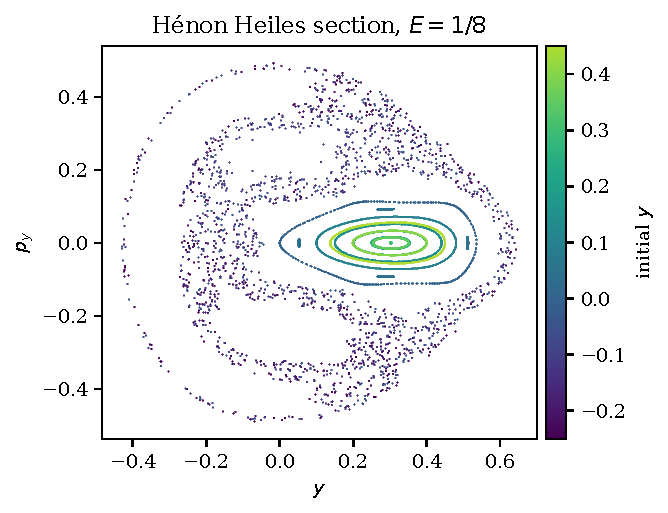
\includegraphics[width=0.78\textwidth]{henon_heiles}
\caption{Poincar\'e's surface of section for the H\'enon Heiles system at $E=1/8$, crossing $x=0$ with $p_x>0$. Fifteen orbits, started at $x=0$ and $p_y=0$ with $y$ equally spaced from $-0.25$ to $0.45$ and followed to time $2500$, are colored by initial $y$. Ten lie on invariant curves and five wander through a chaotic region.}
\label{fig:hh}
\end{figure}

\section{The recurrence theorem}

\begin{theorem}[Poincar\'e recurrence]
\label{thm:recurrence}
Let $(X,\mathcal{B},\mu)$ be a probability space and $T:X\to X$ a measurable map preserving $\mu$. For every $A\in\mathcal{B}$, almost every point of $A$ returns to $A$ infinitely often:
\[
\mu\big(\{x\in A: T^n x\in A \text{ for infinitely many } n\}\big) = \mu(A).
\]
\end{theorem}

\begin{proof}
Let $B = \{x\in A: T^n x\notin A \text{ for all } n\geq 1\}$. The sets $T^{-k}B$, $k\geq 0$, are pairwise disjoint: if $x\in T^{-j}B\cap T^{-k}B$ with $j<k$, then $y=T^j x\in B\subset A$ and $T^{k-j}y = T^k x\in B\subset A$, contradicting $y\in B$. Since $\mu(T^{-k}B) = \mu(B)$ and the total mass is one, $\sum_k \mu(B)\leq 1$ forces $\mu(B)=0$. A point $x\in A$ that returns to $A$ only finitely often has a last visit time $n\geq0$, where $n=0$ if it never returns, and then $T^n x\in B$. The set of such points is contained in $\bigcup_{n\geq0}T^{-n}B$, which is null.
\end{proof}

Poincar\'e proved the theorem for volume preserving flows in the memoir on the three body problem~\cite{poincare1890}, and Carath\'eodory gave a short proof for a general invariant measure~\cite{caratheodory1919}. For a Hamiltonian flow on a compact energy surface, Liouville's theorem supplies the invariant measure, and recurrence follows. Poincar\'e drew the consequence for kinetic theory in 1893~\cite{poincare1893}: a gas in a box, started from a state of low entropy, will return arbitrarily close to that state, and so the entropy cannot increase forever. In 1896 Ernst Zermelo, then Planck's assistant, turned this into a formal objection to Boltzmann's H theorem~\cite{zermelo1896}. Boltzmann's reply was that the recurrence times are so long as to be irrelevant. Kac made the reply quantitative~\cite{kac1947}.

\begin{theorem}[Kac's lemma]
\label{thm:kac_lemma}
Let $(X,\mathcal{B},\mu)$ be a probability space and $T:X\to X$ a measurable map preserving $\mu$ that is ergodic: every $B\in\mathcal{B}$ with $\mu(T^{-1}B\,\triangle\,B)=0$ has $\mu(B)\in\{0,1\}$ (Chapter~\ref{ch:ergodic} develops the notion). Let $A\in\mathcal{B}$ with $\mu(A)>0$ and let $\tau_A(x) = \inf\{n\geq 1: T^n x\in A\}$. Then
\[
\int_A \tau_A \dd\mu = 1,\qquad\text{equivalently}\qquad \E_\mu\big[\tau_A\mid A\big] = \frac{1}{\mu(A)},
\]
where $\E_\mu[\,\cdot\mid A]$ is the expectation under $\mu$ conditioned on $A$.
\end{theorem}

\begin{proof}
Let $S = \bigcup_{n\geq0}T^{-n}A$ be the set of points that enter $A$ at some time. Then $T^{-1}S\subset S$ and $\mu(T^{-1}S) = \mu(S)$, so $\mu(T^{-1}S\,\triangle\,S) = 0$. Since $S\supset A$ and $\mu(A)>0$, ergodicity gives $\mu(S) = 1$.

Let $\varphi(x) = \inf\{n\geq0:T^nx\in A\}$ be the entry time into $A$, so that $\{\varphi<\infty\} = S$ and $\{\varphi = 0\} = A$. Comparing the first visit to $A$ from $x$ with the first visit from $Tx$ gives $\tau_A(x) = 1+\varphi(Tx)$ for $x\in A$ and $\varphi(x) = 1+\varphi(Tx)$ for $x\notin A$. Put $E_k = \{\varphi = k\}$. The second relation says $E_{k+1} = T^{-1}E_k\setminus A$, and the first says $A\cap T^{-1}E_k = A\cap\{\tau_A = k+1\}$. Since $\mu(T^{-1}E_k) = \mu(E_k)$,
\[
\mu(E_{k+1}) = \mu(E_k) - \mu\big(A\cap\{\tau_A = k+1\}\big).
\]
As $\mu(E_0) = \mu(A) = \mu(A\cap\{\tau_A>0\})$, induction gives $\mu(E_k) = \mu(A\cap\{\tau_A>k\})$ for every $k\geq0$. Summing over $k$,
\[
1 = \mu(S) = \sum_{k\geq0}\mu(E_k) = \sum_{k\geq0}\mu\big(A\cap\{\tau_A>k\}\big) = \int_A\tau_A\dd\mu.
\]
The conditional form follows by dividing by $\mu(A)$. Ergodicity was used only to obtain $\mu(S) = 1$. Without it the computation gives $\int_A\tau_A\dd\mu = \mu(S)$, which for the identity map of a two point space with the uniform measure and $A$ one of the points is $\tfrac12$.
\end{proof}

For a mole of gas, the set of microstates in which, say, all molecules lie in the left half of the box has relative measure about $2^{-6\times 10^{23}}$. If the time one map $T$ of the gas is ergodic, Theorem~\ref{thm:kac_lemma} says that the expected return time to this set from a start in it is the reciprocal, $2^{6\times10^{23}}$ steps of $T$, a number with about $1.8\times10^{23}$ decimal digits, whereas the number of atoms in the observable universe, about $10^{80}$, has 81. Recurrence is a theorem; it is also irrelevant on every physical time scale. Chapter~\ref{ch:kinetic} treats an exactly solvable model, Kac's ring, in which the recurrence time is $2N$ and Boltzmann's law holds for times that are short compared with it (Figure~\ref{fig:kacring}). The ring map is a permutation of period $2N$ and is not ergodic, so Theorem~\ref{thm:kac_lemma} does not apply to it.

\section{The method of arbitrary functions}

How does chance arise in a deterministic world? Poincar\'e's answer, given in an essay of 1899~\cite{poincare1899} and in the second edition of the \emph{Calcul des probabilit\'es}~\cite{poincare1912calcul}, used a roulette wheel. The wheel is divided into many equal sectors, alternately red and black. The croupier gives it an initial velocity, and the final position is a deterministic but extremely sensitive function of that velocity. Poincar\'e argued that whatever the distribution of initial velocities, provided it is reasonably smooth, the probability of red will be close to one half. The probability is not in the dynamics and not in the croupier; it emerges from the interaction of a smooth density with a rapidly oscillating map. Borel gave the method a chapter of its own in a textbook of 1909~\cite{borel1909elements} and observed that continuity of the density suffices, Fr\'echet reduced the requirement to Riemann integrability in 1921~\cite{frechet1921}, Hopf recast it in the 1930s as a statement about the long time behavior of dynamical systems, related to mixing~\cite{hopf1934}, and Engel gave a comprehensive treatment~\cite{engel1992}. The following sharp version is elementary.

\begin{theorem}[Arbitrary functions]
\label{thm:arbitrary}
Let $X$ be a real random variable with density $g$ of total variation $V<\infty$. For $t>0$ and $a\in[0,1]$,
\[
\Big|\,\P\big(\{tX\}\in[0,a)\big) - a\,\Big|\leq \frac{a(1-a)\,V}{2t},
\]
where $\{\cdot\}$ denotes the fractional part. The bound is attained: for the uniform density on $[0,1]$, which has $V=2$, the error equals $a(1-a)/t$ whenever $t-a$ is a nonnegative integer.
\end{theorem}

\begin{proof}
For $a\in\{0,1\}$ both sides vanish, so let $0<a<1$. Partition $\R$ into the cells $I_n = [n/t,(n+1)/t)$ and split each into $I_n' = [n/t,(n+a)/t)$ and $I_n'' = [(n+a)/t,(n+1)/t)$, of lengths $a/t$ and $(1-a)/t$. Let $\bar g_n'$ and $\bar g_n''$ be the averages of $g$ over $I_n'$ and $I_n''$. Since $\{tX\}\in[0,a)$ exactly when $X\in I_n'$ for some $n$, and $\sum_n\int_{I_n}g = 1$,
\[
\begin{aligned}\P(\{tX\}\in[0,a)) - a &= \sum_{n\in\Z}\Big(\int_{I_n'}g - a\int_{I_n}g\Big)\\
&= \frac{a(1-a)}{t}\sum_{n\in\Z}\big(\bar g_n'-\bar g_n''\big),\end{aligned}
\]
where the last step uses $\int_{I_n'}g = \frac at\bar g_n'$ and $\int_{I_n}g = \frac at\bar g_n'+\frac{1-a}t\bar g_n''$. A density of bounded variation tends to zero at $\pm\infty$, so its Jordan decomposition is $g = g_+-g_-$ with $g_\pm$ nondecreasing and each of total increase $V/2$. For a nondecreasing function $h$ the average over $I_n'$ is at most $h((n+a)/t)$, the average over $I_n''$ is at least $h((n+a)/t)$, and both lie between the infimum and the supremum of $h$ over $I_n$. Hence $-\Delta_nh\leq\bar h_n'-\bar h_n''\leq0$, where $\Delta_nh$ is the increase of $h$ over $I_n$. Applied to $g_+$ and $g_-$ this gives $-\Delta_ng_+\leq\bar g_n'-\bar g_n''\leq\Delta_ng_-$, and since $\sum_n\Delta_ng_\pm\leq V/2$, the sum over $n$ has absolute value at most $V/2$.
\end{proof}

Theorem~\ref{thm:arbitrary} is an early and simple instance of a result that derives a probability law from a deterministic dynamics: the output law is insensitive to the input law, which may be regarded as a prior, because the dynamics stretches phase space. The rate $1/t$ can be improved for smoother densities. If $g$ is continuously differentiable and $g'$ has bounded variation $V'$, the Poisson summation formula gives $\P(\{tX\}\in[0,a)) - a = \sum_{k\neq0}\frac{e^{2\pi ika}-1}{2\pi ik}\,\hat g(kt)$, where $\hat g(\xi) = \int g(x)e^{-2\pi ix\xi}\dd x$, and two integrations by parts give $|\hat g(\xi)|\leq V'/(4\pi^2\xi^2)$. The error is then at most $\zeta(3)V'/(2\pi^3t^2)$. Poincar\'e insisted that every probability statement rests on a convention, a choice of prior; the method of arbitrary functions explains why, in physics, the choice often does not matter.

\section{Poincar\'e and inverse probability}

Poincar\'e was a Bayesian in the precise sense that he regarded the probability of causes as the fundamental problem of applied probability and held that it cannot be solved without a prior. In \emph{La science et l'hypoth\`ese} (1902) Poincar\'e calls the problems of the probability of causes the most important from the point of view of scientific applications and the essential problem of the experimental method~\cite{poincare1902}. The book states that the probability of a cause, given the observed effect, could not be calculated if a more or less justified convention did not supply in advance the probability of the cause, and that without such a convention the problem would have no meaning. The same reasoning applies to the inference of a physical law from observations: a curve drawn through measured points is the most probable law only because a regular law is judged more probable beforehand than an irregular one.

The most dramatic application was legal. In the Dreyfus affair the handwriting expert Alphonse Bertillon had argued, with a pseudo mathematical analysis of coincidences in the \emph{bordereau}, that Dreyfus was its author. Poincar\'e's letter, read at the Rennes court martial in 1899, criticized Bertillon's work for its lack of scientific foundation~\cite{mazliak2012}. In 1904 the Cour de cassation asked Darboux, Appell and Poincar\'e for a full report~\cite{darboux1904}. It opens with a short chapter on the probability of causes, which Mansuy and Mazliak describe as a small course on the correct use of the Bayes formula~\cite{mansuymazliak2005}. The report shows that Bertillon had computed the probability of four coincidences as $(0.2)^4$, which is the probability that four specified trials all produce a coincidence, whereas the probability of four coincidences among the twenty six trials available, which the report puts at about $0.7$, is some four hundred times larger, and that coincidences chosen because they were noticed prove nothing. It explains with two urns that the question is the probability of a cause given an observed effect, here forgery or natural writing, and that answering it requires the probability of the cause before the evidence. The authors held that in a question of this kind the prior is made of moral elements that escape calculation. They gave no probability of forgery and said only that the coincidences multiply the odds on forgery by some factor. The verdict against Dreyfus was annulled in 1906.

Poincar\'e also recorded the famous remark, which he attributed to Lippmann, that everyone believes in the normal law of errors: the experimenters because they think it is a theorem of mathematics, and the mathematicians because they think it is an experimental fact~\cite{poincare1912calcul}. The remark is a joke about foundations, and the sixth problem is the request to take the joke seriously. The central limit theorem, the maximum entropy characterization and the Maxwell characterization by rotation invariance and independence are three different mathematical reasons for the normal law, and each corresponds to a different physical hypothesis.

\section{Poincar\'e and Bachelier}

Poincar\'e's report on Bachelier's thesis~\cite{bachelier1900}, written in 1900, is short and appreciative~\cite{courtault2000}. He noted the originality of the approach, praised the derivation of the law of the price by a reasoning analogous to Fourier's theory of heat, and observed that the topic was somewhat removed from those usually treated by candidates. The thesis received the grade \emph{honorable}, which was respectable but not the highest~\cite{taqqu2001}. Bachelier's later career was difficult, and the work was largely neglected until Kolmogorov cited it in 1931~\cite{kolmogorov1931}. Samuelson, alerted by Savage, brought it to the attention of economists in the 1950s~\cite{taqqu2001}.

Bachelier showed that the probability density of a price with independent increments satisfies what he called the equation of radiation of probability, the heat equation. This is an early and influential appearance of the idea that a macroscopic diffusion is the law of a microscopic random motion, the idea Einstein made physical in 1905~\cite{einstein1905} and that Chapter~\ref{ch:brownian} develops.

\section{The quantum and the end of continuity}

In 1911 Poincar\'e attended the first Solvay conference in Brussels, devoted to radiation and the quanta. Returning to Paris he set himself a precise question: is the quantum hypothesis necessary to obtain Planck's law of black body radiation, or might a continuous mechanics with a suitable distribution of energies suffice? In a long paper of 1912~\cite{poincare1912quanta} he showed that it is necessary. The mathematical core is a uniqueness theorem for Laplace transforms. Let $\sigma$ be the measure on $[0,\infty)$ that describes how many states of a resonator of frequency $\nu$ have a given energy, so that at inverse temperature $\beta$ the partition function is $Z(\beta)=\int e^{-\beta E}\sigma(\dd E)$ and the mean energy is $-\frac{\dd}{\dd\beta}\log Z(\beta)$. Planck's law says that the mean energy is $h\nu/(e^{\beta h\nu}-1)$, where $h$ is Planck's constant. Integrating, $Z(\beta)=c\,(1-e^{-\beta h\nu})^{-1}=c\sum_{j\geq0}e^{-\beta jh\nu}$ for a constant $c$, and since a measure on $[0,\infty)$ is determined by its Laplace transform, $\sigma=c\sum_{j\geq0}\delta_{jh\nu}$: the energy of the resonator is concentrated on integer multiples of $h\nu$. A continuous distribution of energies, for which $\sigma$ has a density, cannot produce Planck's law, and the classical choice $\sigma(\dd E)\propto\dd E$ gives the mean energy $1/\beta$ and the Rayleigh Jeans law. Poincar\'e's own proof treats resonators exchanging energy with molecules at fixed total energy and is more delicate~\cite{prentis1995,mccormmach1967}, but it is a statement of the same kind about the support of a measure inferred from an observed law, and in that sense it is an inverse problem in exactly our sense. Ehrenfest reached a related conclusion in 1911~\cite{ehrenfest1911quanta}. Poincar\'e died in July 1912, a few months later. Chapter~\ref{ch:quantum} takes up the axiomatization of the quantum theory.

\section{The Poincar\'e inequality}

The rate at which a diffusion forgets its initial state is controlled by an inequality that bears Poincar\'e's name, after his 1890 paper on the partial differential equations of mathematical physics~\cite{poincare1890b}. The Gaussian case was proved by Nash~\cite{nash1958} and Chernoff~\cite{chernoff1981} with Hermite polynomials; the proof below uses the Ornstein Uhlenbeck semigroup instead.

\begin{theorem}[Gaussian Poincar\'e inequality]
\label{thm:gaussian_poincare}
Let $\gamma$ be the standard Gaussian measure on $\R^n$. For every $f\in L^2(\gamma)$ with weak gradient in $L^2(\gamma)$,
\[
\Var_\gamma(f)\leq \int |\nabla f|^2 \dd\gamma,
\]
with equality for linear $f$.
\end{theorem}

\begin{proof}
It suffices to prove the inequality for smooth $f$ such that $f$ and $\nabla f$ have polynomial growth: these functions are dense in the class of the statement for the norm $(\int f^2\dd\gamma+\int|\nabla f|^2\dd\gamma)^{1/2}$, and both sides of the inequality are continuous for that norm. Let $(P_t)$ be the Ornstein Uhlenbeck semigroup, $P_t f(x) = \E f(e^{-t}x + \sqrt{1-e^{-2t}}\,Z)$ with $Z\sim\gamma$. It is symmetric in $L^2(\gamma)$, has generator $\mathcal{L}f = \Delta f - x\cdot\nabla f$, satisfies $\int f\,\mathcal{L}f\dd\gamma = -\int|\nabla f|^2\dd\gamma$, and $P_t f\to\int f\dd\gamma$ in $L^2(\gamma)$. Differentiating under the integral sign gives the commutation $\nabla P_t f = e^{-t}P_t\nabla f$, and Jensen's inequality gives $|\nabla P_t f|^2\leq e^{-2t}P_t|\nabla f|^2$. Hence
\[
\begin{aligned}\Var_\gamma(f) &= -\int_0^\infty \frac{\dd}{\dd t}\int (P_t f)^2\dd\gamma\dd t\\
&= 2\int_0^\infty\!\!\int |\nabla P_t f|^2\dd\gamma\dd t\\
&\leq 2\int_0^\infty e^{-2t}\dd t\int |\nabla f|^2\dd\gamma,\end{aligned}
\]
using invariance $\int P_t g\dd\gamma = \int g\dd\gamma$. For $f(x) = a\cdot x$ both sides equal $|a|^2$.
\end{proof}

\begin{corollary}[Exponential convergence to equilibrium]
For the Ornstein Uhlenbeck semigroup, $\|P_t f - \int f\dd\gamma\|_{L^2(\gamma)}\leq e^{-t}\|f - \int f\dd\gamma\|_{L^2(\gamma)}$.
\end{corollary}

\begin{proof}
Write $h(t) = \Var_\gamma(P_t f)$. Then $h'(t) = -2\int |\nabla P_t f|^2\dd\gamma\leq -2h(t)$ by the theorem applied to $P_t f$, and Gr\"onwall's lemma gives $h(t)\leq e^{-2t}h(0)$.
\end{proof}

The best constant $C$ in a Poincar\'e inequality $\Var_\pi(f)\leq C\,\mathcal{E}(f,f)$, where $\mathcal{E}(f,f) = -\int f\,\mathcal{L}f\dd\pi$ is the Dirichlet form of the generator, is the reciprocal of the spectral gap $\lambda_1$ of $-\mathcal{L}$; for the Ornstein Uhlenbeck process both equal one. Poincar\'e inequalities and their logarithmic strengthening, the log Sobolev inequality of Theorem~\ref{thm:lsi}, give the rates of convergence to equilibrium for the Ornstein Uhlenbeck flow in Chapter~\ref{ch:entropy} and for Kac's model in Chapter~\ref{ch:kinetic}. The same constant governs the efficiency of Markov chain Monte Carlo: for a reversible chain the asymptotic variance of an ergodic average is at most $(2/\lambda_1-1)\Var_\pi(f)$, where $\lambda_1$ is the spectral gap of the chain (Chapter~\ref{ch:ergodic}), so a Poincar\'e constant is a statement about how much computation inference costs.

\section{The conjecture and Perelman's entropy}

In the fifth supplement to \emph{Analysis Situs}, published in 1904~\cite{poincare1904}, Poincar\'e asked whether a closed three dimensional manifold with trivial fundamental group must be homeomorphic to the three sphere. The question became the most famous problem in topology. Hamilton proposed in 1982 to attack it with the Ricci flow $\partial_t g = -2\Ric(g)$, a nonlinear heat equation for the metric~\cite{hamilton1982}. Perelman completed the program in three preprints of 2002 and 2003~\cite{perelman2002,perelman2003a,perelman2003b}, and the first of them introduced a functional that Perelman called an entropy. Let $(M,g)$ be a closed $n$ dimensional Riemannian manifold with scalar curvature $R$ and Riemannian volume element $\dd\,\mathrm{vol}$, let $f$ be a smooth function on $M$ and let $\tau>0$, with $f$ normalized by $\int_M(4\pi\tau)^{-n/2}e^{-f}\dd\,\mathrm{vol} = 1$. Perelman's functional is
\[
\mathcal{W}(g,f,\tau) = \int_M \big[\tau\big(R + |\nabla f|^2\big) + f - n\big]\,(4\pi\tau)^{-n/2}e^{-f}\dd\,\mathrm{vol}.
\]
Perelman remarked on the analogy with Boltzmann's entropy and with the thermodynamics of the heat kernel. In Chapter~\ref{ch:entropy} we show that on flat space $\mathcal{W}$ is exactly the combination of Shannon entropy and Fisher information that appears in de Bruijn's identity, that its monotonicity along the heat flow is a probabilistic statement about Gaussian convolution, and that its nonnegativity is the log Sobolev inequality (Theorem~\ref{thm:perelman_flat}). On a curved manifold $\mathcal{W}$ also contains the scalar curvature, which is why the identification with Shannon entropy and Fisher information holds only on flat space. Perelman's proof of the conjecture uses the monotonicity of $\mathcal{W}$ to show that the Ricci flow does not collapse locally, and then needs surgery at singular times~\cite{perelman2003a} and the finite extinction time of the flow~\cite{perelman2003b}; Kleiner and Lott give a detailed exposition of the first two preprints~\cite{kleinerlott2008}.

\section{Poincar\'e's shuffles: random walks on groups}

The second edition of \emph{Calcul des probabilit\'es}~\cite{poincare1912calcul} contains, in a chapter of miscellaneous questions added in 1912, a discussion of card shuffling that anticipates the modern theory of random walks on groups. Poincar\'e asked why repeated shuffles produce a deck in which every order is equally likely, and he answered by an argument from the theory of groups that refers to the work of Frobenius and Cartan; Mazliak~\cite{mazliak2012} describes it. The modern form is the following theorem.

\begin{theorem}[Convergence of random walks on finite groups]
\label{thm:random_walk_groups}
Let $G$ be a finite group and $Q$ a probability measure on $G$. The convolution powers $Q^{*n}$ converge to the uniform distribution $U$ on $G$ if and only if the support of $Q$ generates $G$ and is not contained in a coset of a proper normal subgroup. In that case, for every irreducible unitary representation $\rho\neq1$ the Fourier transform $\hat Q(\rho) = \sum_gQ(g)\rho(g)$ has spectral radius strictly less than one. Moreover, with $\|\mu-\nu\|_{TV} = \max_A|\mu(A)-\nu(A)|$,
\[
\|Q^{*n}-U\|_{TV}^2\leq\frac14\sum_{\rho\neq1}d_\rho\,\tr\big(\hat Q(\rho)^n(\hat Q(\rho)^n)^*\big),
\]
where the sum runs over the nontrivial irreducible unitary representations of $G$ up to equivalence and $d_\rho$ is the dimension of $\rho$.
\end{theorem}

\begin{proof}
If the support of $Q$ lies in a proper subgroup $H$, or in a coset $aN$ of a proper normal subgroup $N$, then $Q^{*n}$ gives mass one to $H$, or to the coset $a^nN$, which has $U$ mass at most $\frac12$. Then $\|Q^{*n}-U\|_{TV}\geq\frac12$ for every $n$, and there is no convergence. Now assume that the support generates $G$ and lies in no coset of a proper normal subgroup, and let $\rho\neq1$ be irreducible and unitary. Then $\hat Q(\rho)$ is a contraction. Suppose $\hat Q(\rho)v = \lambda v$ with $|\lambda| = 1$ and $|v| = 1$. Since $\lambda v$ is an average of the unit vectors $\rho(g)v$ for $g$ in the support, and the unit ball of a Hilbert space is strictly convex, $\rho(g)v = \lambda v$ for every $g$ in the support. Every element of the finite group $G$ is a product of elements of the support, so $v$ is an eigenvector of every $\rho(g)$. Irreducibility forces $\dim\rho = 1$, so $\rho$ is a nontrivial character $\chi$ with $\chi(g) = \lambda$ on the support, which then lies in a coset of the proper normal subgroup $\ker\chi$, contrary to assumption. Hence $\hat Q(\rho)$ has spectral radius less than one and $\hat Q(\rho)^n\to0$. The Fourier transform turns convolution into multiplication, $\widehat{Q^{*n}}(\rho) = \hat Q(\rho)^n$, and $\hat U(\rho) = 0$ for $\rho\neq1$. The displayed bound is the upper bound lemma of Diaconis and Shahshahani~\cite{diaconisshahshahani1981,diaconis1988}: Cauchy Schwarz turns total variation into an $L^2$ distance, and the Plancherel theorem for $G$ expresses the latter in terms of Fourier coefficients. Its right side is a finite sum of terms that tend to zero.
\end{proof}

The spectral radius cannot be replaced by the operator norm. On $S_3$ the measure uniform on $\{(12),(123)\}$ satisfies the conditions of the theorem, so it converges to uniform, but $\hat Q(\rho)$ has operator norm one on the two dimensional representation, with spectral radius $\frac12$. Poincar\'e did not compute rates, but the structure of his argument, a spectral gap on each nontrivial representation, is in our reading that of the theorem. Diaconis and Shahshahani showed in 1981 that random transpositions mix a deck of $n$ cards after about $\frac12n\log n$ steps~\cite{diaconisshahshahani1981}, and Bayer and Diaconis showed in 1992 that seven riffle shuffles suffice for a deck of fifty two~\cite{bayerdiaconis1992}. The method of arbitrary functions explains how a physical process forgets its initial condition; the random walk theorem explains how a sequence of independent randomizations forgets it. Both are theorems about convergence to a uniform law, and both are ancestors of the Markov chain Monte Carlo methods of Chapter~\ref{ch:spins}.

\section{The Maxwell, Poincar\'e and Borel lemma}

\begin{theorem}[Maxwell, Poincar\'e and Borel]
\label{thm:sphere_lemma}
Let $X^{(n)}$ be uniformly distributed on the sphere $\{x\in\R^n:|x|^2 = n\}$. For each fixed $k$ the law of the first $k$ coordinates $(X^{(n)}_1,\dots,X^{(n)}_k)$ converges in total variation to the standard Gaussian law on $\R^k$.
\end{theorem}

\begin{proof}
Let $Z$ be standard Gaussian in $\R^n$. By rotation invariance, $X^{(n)}\eqd\sqrt n\,Z/|Z|$. The first $k$ coordinates equal $Z_{1:k}\cdot\sqrt{n}/|Z|$, and $|Z|^2/n\to1$ almost surely by the law of large numbers. This gives convergence in law. For total variation, let $n>k$. The first $k$ coordinates have the density
\[
\begin{aligned}f_n(x) &= c_{n,k}\Big(1-\frac{|x|^2}{n}\Big)^{(n-k-2)/2},\quad |x|^2<n,\\
c_{n,k} &= \frac{\Gamma(n/2)}{(\pi n)^{k/2}\,\Gamma((n-k)/2)},\end{aligned}
\]
obtained by integrating over the sphere of radius $\sqrt{n-|x|^2}$ in $\R^{n-k}$, where $c_{n,k}$ is the constant that makes $f_n$ a probability density. By Stirling's formula $\Gamma(n/2)/\Gamma((n-k)/2)\sim(n/2)^{k/2}$, so $c_{n,k}\to(2\pi)^{-k/2}$, and $(1-|x|^2/n)^{(n-k-2)/2}\to e^{-|x|^2/2}$. Hence $f_n$ converges pointwise to the standard Gaussian density on $\R^k$. Since all these functions are probability densities, Scheff\'e's lemma upgrades pointwise convergence to convergence in total variation.
\end{proof}

The lemma is the microcanonical derivation of the Maxwellian: a gas with fixed total kinetic energy, uniformly distributed over the energy sphere, has Gaussian one particle velocities in the limit. It also underlies Kac's model in Chapter~\ref{ch:kinetic}, whose state space is exactly this sphere, and it is a relative of the concentration of measure phenomenon that L\'evy studied and that Milman later made a pillar of high dimensional geometry. The result is usually attributed to Poincar\'e, but Diaconis and Freedman could not find it in Poincar\'e's work~\cite{diaconisfreedman1987}. The earliest probabilistic statement they located is in Borel~\cite{borel1914}, who had studied the uniform measure on a ball of velocities in 1906~\cite{borel1906}, and they point to Maxwell for the idea. Their quantitative version gives a total variation bound of order $k/n$, the rate of the finite de Finetti theorem of Chapter~\ref{ch:axioms} for finitely many values.

\section{Poincar\'e on kinetic theory}

The paper of 1906, \emph{R\'eflexions sur la th\'eorie cin\'etique des gaz}~\cite{poincare1906}, examines the argument of Gibbs for the second law~\cite{gibbs1902} and distinguishes two hypotheses about probability. In the discontinuous hypothesis one has a very large number of similar systems, such as the molecules of a one dimensional gas, whose initial states are known exactly, and the probability of a region of phase space is the fraction of the systems that lie in it. In the continuous hypothesis the initial state of a single system is known only through a probability density. Under the first hypothesis the entropy integral is infinite, and the paper adopts the second. It also distinguishes the fine entropy, the limit of the cell entropies as the cells shrink, from the coarse entropy computed with cells so small that ordinary methods of observation cannot tell two states within a cell apart. It proves that the fine entropy is constant in time, so that any increase must come from coarse graining, and that, in the sign convention in which entropy increases, the coarse entropy is never smaller than the fine entropy. Gibbs had made the same point in the \emph{Elementary Principles}~\cite[Chapter~XII]{gibbs1902} with the picture of a coloring matter stirred through an incompressible liquid: its density measured on cells of fixed size tends to a uniform limit, although the density carried along with the liquid never changes.

These remarks are consistent with the structure of Lanford's theorem (Theorem~\ref{thm:lanford})~\cite{lanford1975}. The Boltzmann entropy that increases is the entropy of the one particle marginal, a coarse grained quantity; the Gibbs entropy of the full $N$ particle law is conserved; and the difference between them measures correlations created by collisions, which are invisible in the limit because they concentrate on a set of vanishing measure. In the language of Chapter~\ref{ch:axioms}, chaos is lost at finite $N$ and recovered in the limit, and Poincar\'e's two hypotheses correspond to the empirical measure of one gas and the de Finetti measure over gases.

\section{Poincar\'e and the theory of errors}

Poincar\'e's \emph{Calcul des probabilit\'es}~\cite{poincare1912calcul} also contains a careful discussion of Gauss's derivation of the normal law of errors. Gauss had shown in 1809~\cite{gauss1809} that if the arithmetic mean is always the most probable value of a location parameter, then the error law must be Gaussian. Poincar\'e examined the argument, noted that it presupposes a uniform prior on the location, and gave a version in which the prior is explicit and, with enough observations, does not affect the conclusion; Mazliak~\cite{mazliak2012} describes this analysis. It is an early instance of the observation that characterizations of the normal law by the optimality of the sample mean are statements about Bayes estimators under flat priors. In modern terms, the Gaussian is the only location family for which the sample mean is the maximum likelihood estimate of the location for every sample size, and under a flat prior the maximum likelihood estimate is the posterior mode. Teicher gave a rigorous proof that needs only continuity of the density and the property for samples of sizes two and three~\cite{teicher1961}. The three reasons for the normal law listed earlier in this chapter are thereby joined by a fourth, Gauss's: the Gaussian is the error law that makes averaging optimal.

\section{Poincar\'e and Hilbert}

Hilbert and Poincar\'e represented different philosophies of foundations. Hilbert's axiomatic method sought consistent formal systems from which theories could be deduced. Poincar\'e's conventionalism held that the axioms of geometry and mechanics are neither synthetic truths nor experimental facts but conventions, chosen for convenience and guided by experience; and he distrusted the formal turn in logic, which he satirized in his debates with Russell and Couturat. Yet on the sixth problem their views converge more than they diverge. Hilbert asked for the limiting process from atoms to continua. Poincar\'e had shown that the approach to equilibrium cannot hold for every initial condition, because of recurrence and reversibility, and that statements of this kind can hold for every smooth probability law on the initial conditions, as the method of arbitrary functions shows. The paper of 1906 makes the point for a very large number of small planets on circular orbits: the longitudes become uniformly distributed for every smooth law of the initial data, the recurrence time grows with the number of planets and is infinite in the limit, and an initial distribution that is not smooth, such as planets placed on a line, leaves a latent organization, a spiral wound too tightly to be seen, which a coarse observer takes for uniformity~\cite{poincare1906}. Boltzmann answered the objections of Loschmidt and Zermelo by moving from individual trajectories to probabilities. The modern answer to Hilbert, a limit theorem for the empirical measure under a probability law on initial conditions, as the number of particles grows and the time is held fixed, is due to Kac~\cite{kac1956} and, for hard spheres, Lanford~\cite{lanford1975} (Chapter~\ref{ch:kinetic}); it joins Hilbert's limit with Poincar\'e's probability measures.

The Bayesian reading adds one more convention to Poincar\'e's list: the prior on initial conditions. Poincar\'e had written that the probability of causes requires a hypothesis about prior probabilities; we add that the hypothesis can be checked, refined and computed with, and that the method of arbitrary functions explains when it washes out.

\section*{Exercises}
\begin{enumerate}
\item For the circle rotation $x\mapsto x+\alpha$ modulo one with $\alpha$ irrational, verify recurrence directly and compute the expected return time to an interval of length $\delta$ started uniformly in it.
\item Let $X$ be exponential with rate $\lambda$. Compute $\P(\{tX\}<\frac12)$ exactly and compare the error with the bound of Theorem~\ref{thm:arbitrary}.
\item Show that the Gaussian Poincar\'e inequality is an equality for the Hermite polynomial of degree one, and compute the ratio $\int|f'|^2\dd\gamma/\Var_\gamma(f)$ for the Hermite polynomial $\mathrm{He}_k$ of degree $k$ on $\R$.
\item Let $Q$ on $S_3$ give weight $\frac13$ to the identity and $\frac29$ to each of the three transpositions. Compute $\hat Q(\rho)$ for the two dimensional irreducible representation and for the sign representation, and find the rate of convergence to uniform. Explain why the walk that picks one of the three transpositions uniformly does not converge.
\item Derive the density of the first $k$ coordinates of a uniform point on the sphere of radius $\sqrt n$ in $\R^n$.
\end{enumerate}


\section*{Notes}

Barrow Green~\cite{barrowgreen1997} tells the story of the King Oscar prize and the error in detail. Gray~\cite{gray2013} is a scientific biography of Poincar\'e. The Darboux, Appell and Poincar\'e report on Bertillon~\cite{darboux1904} is introduced by Mansuy and Mazliak~\cite{mansuymazliak2005}; Taroni, Champod and Margot~\cite{taroni1998} survey the early history of Bayesian reasoning in forensic science. We have paraphrased the report's argument. Poincar\'e's quantum paper is analyzed by McCormmach~\cite{mccormmach1967} and Prentis~\cite{prentis1995}. Mazliak~\cite{mazliak2012} surveys Poincar\'e's work on probability. For the method of arbitrary functions see von Plato~\cite{vonplato1994} and Engel~\cite{engel1992}; Diaconis, Holmes and Montgomery~\cite{diaconis2007coin} apply the same reasoning to coin tossing and find a small but real bias toward the side facing up.

\chapter[Axioms of Probability and Large Deviations]{Axioms of Probability and Large Deviations: Kolmogorov, de Finetti and Sanov}
\label{ch:axioms}

\section{Before 1933}

When Hilbert asked for a logical development of the calculus of probabilities, the subject had no agreed definition of its basic objects. Laplace had defined probability as the ratio of favorable to equally possible cases, which is circular. Venn and later von Mises defined it as a limiting frequency in an infinite sequence, a \emph{Kollektiv}, which raises the question of which sequences qualify. Borel had shown in 1909~\cite{borel1909} that the strong law of large numbers for binary digits can be proved with Lebesgue measure, and Lebesgue's integral of 1902~\cite{lebesgue1902} supplied the analytic tool. What was missing was the recognition that probability theory could simply \emph{be} measure theory on a space of total mass one, with independence and conditioning defined inside that framework.

\section{Kolmogorov's axioms}

\begin{definition}[Probability space]
A probability space is a triple $(\Omega,\mathcal{F},\P)$ where $\Omega$ is a set, $\mathcal{F}$ a $\sigma$ algebra of subsets of $\Omega$, and $\P:\mathcal{F}\to[0,1]$ a countably additive function with $\P(\Omega)=1$. A random variable is a measurable map $X:\Omega\to E$ into a measurable space; its law is the image measure $\P\circ X^{-1}$.
\end{definition}

Kolmogorov's \emph{Grundbegriffe}~\cite{kolmogorov1933} contains five axioms for a field of events and a sixth, the continuity axiom, equivalent to countable additivity. Its decisive contributions are two theorems.

\begin{theorem}[Kolmogorov extension]
\label{thm:kolmogorov_extension}
Let $E$ be a Polish space and, for each finite $J\subset I$ of an arbitrary index set $I$, let $\mu_J$ be a probability measure on $E^J$. If the family is consistent, meaning that the image of $\mu_K$ under the coordinate projection $E^K\to E^J$ is $\mu_J$ whenever $J\subset K$, then there is a unique probability measure $\mu$ on the product $\sigma$ algebra of $E^I$ whose finite dimensional marginals are the $\mu_J$.
\end{theorem}

Kolmogorov proved the theorem for real valued coordinates~\cite[Chapter~III, Section~4]{kolmogorov1933}. The proof carries over to Polish spaces because every Borel probability measure on a Polish space is tight, and we quote the theorem without proof. The extension theorem is what makes stochastic processes, and therefore Brownian motion and the many particle systems of kinetic theory, legitimate mathematical objects. It also exposes a limitation: the product $\sigma$ algebra on $\R^{[0,1]}$ does not contain the set of continuous paths, which is why Wiener's construction (Chapter~\ref{ch:brownian}) and its modern descendants are needed.

The second contribution is conditional expectation. Given a sub $\sigma$ algebra $\mathcal{G}$ and an integrable $X$, the measure $A\mapsto\E[X\mathbb{1}_A]$ on $\mathcal{G}$ is absolutely continuous with respect to $\P$, and its Radon Nikodym derivative is $\E[X\mid\mathcal{G}]$. With this definition, conditioning on events of probability zero, such as the event that the energy of a gas equals a given value, becomes meaningful through regular conditional distributions. The microcanonical ensemble of statistical mechanics is such a conditional distribution, and Bayesian posteriors for continuous parameters are another.

Kolmogorov regarded the axioms as settling the logical status of probability and leaving its application to experience. In the \emph{Grundbegriffe} he writes that the theory of probability as a mathematical discipline can and should be developed from axioms in exactly the same way as geometry and algebra, and a few lines later he compares the definition of a field of probabilities, whose elements may be given any meaning, with the introduction of basic concepts in Hilbert's \emph{Foundations of Geometry}. The probability half of the sixth problem is, in the axiomatic reading, solved.

\section{De Finetti: coherence and exchangeability}

Bruno de Finetti approached the foundations from the opposite direction. For him probability is a degree of belief, operationally defined by the prices at which an agent will buy and sell bets, and the axioms are consequences of a single requirement: that the agent not accept a combination of bets that loses money in every state of the world~\cite{definetti1937}.

\begin{theorem}[Coherence]
\label{thm:coherence}
Let $A_1,\dots,A_k$ be events in a finite space $\Omega$ and let an agent announce prices $q_1,\dots,q_k$ at which she will buy or sell, in any real quantity, a ticket paying one unit if $A_i$ occurs. There is no combination of stakes $s_1,\dots,s_k$ whose net gain $\sum_i s_i(\mathbb{1}_{A_i}(\omega)-q_i)$ is strictly negative for every $\omega\in\Omega$ if and only if there exists a probability measure $\P$ on $\Omega$ with $\P(A_i) = q_i$ for all $i$.
\end{theorem}

\begin{proof}
If such $\P$ exists, the expected net gain under $\P$ of any stakes is zero, so it cannot be negative everywhere. Conversely let $C\subset\R^k$ be the convex hull of the vectors $a(\omega) = (\mathbb{1}_{A_i}(\omega))_i$, $\omega\in\Omega$. A probability $\P$ with $\P(A_i) = q_i$ exists if and only if $q\in C$. If $q\notin C$, the separating hyperplane theorem for the compact convex set $C$ gives $s\in\R^k$ with $s\cdot(a(\omega)-q)<0$ for all $\omega$, which is a sure loss.
\end{proof}

De Finetti's deeper contribution concerns sequences. A sequence $X_1,X_2,\dots$ is \emph{exchangeable} if its law is invariant under finite permutations of indices. Independent identically distributed sequences are exchangeable, and so are mixtures of them.

\begin{theorem}[de Finetti, Hewitt and Savage]
\label{thm:definetti}
Let $X_1,X_2,\dots$ be an exchangeable sequence with values in a Polish space $E$. There is a unique probability measure $\Pi$ on the space $\mathcal{P}(E)$ of probability measures on $E$ such that for every $n$,
\[
\P(X_1\in A_1,\dots,X_n\in A_n) = \int_{\mathcal{P}(E)} \prod_{i=1}^n Q(A_i)\,\Pi(\dd Q).
\]
Moreover the empirical measures $\frac1n\sum_{i\leq n}\delta_{X_i}$ converge weakly almost surely to a random measure $\tilde Q$ with law $\Pi$.
\end{theorem}

The theorem is the bridge between the subjective and frequentist views: an agent who judges a sequence exchangeable behaves as if there were an unknown parameter $\tilde Q$, drawn from a prior $\Pi$, given which the observations are independent. The parameter is a limit of observables. De Finetti proved the theorem for binary sequences~\cite{definetti1937}, and Hewitt and Savage proved the version for compact Hausdorff spaces and the associated zero one law~\cite{hewittsavage1955}; the version for a Polish space $E$ follows by embedding $E$ in a compact metric space. We quote the theorem without proof for general $E$; the binary case is proved in Section~\ref{sec:binary_definetti}. For finite sequences the representation holds approximately.

\begin{theorem}[Diaconis and Freedman]
\label{thm:diaconis_freedman}
Let $(X_1,\dots,X_n)$ be exchangeable and let $k\leq n$. If the $X_i$ take values in a set of $c$ points, then the law of $(X_1,\dots,X_k)$ is within total variation distance $2ck/n$ of a mixture of independent identically distributed laws. If the $X_i$ take values in a Polish space, the distance is at most $k(k-1)/n$.
\end{theorem}

The distance in the theorem is twice the supremum over events, the normalization of Diaconis and Freedman~\cite{diaconisfreedman1980}. With the supremum, the convention of Appendix~\ref{app:toolkit}, the two bounds are $ck/n$ and $k(k-1)/(2n)$. Diaconis and Freedman give examples showing that neither rate can be improved. We quote the first bound without proof. The second is the birthday bound. Given the empirical measure of $(X_1,\dots,X_n)$, exchangeability makes $(X_1,\dots,X_k)$ a draw of $k$ values without replacement from the $n$ values, and the mixture is the same draw with replacement. The two draws can be coupled to agree unless an index repeats, an event of probability at most $k(k-1)/(2n)$. In kinetic theory $n$ is the number of particles and $k$ the number of particles whose joint law we wish to describe. The one particle space is continuous, so the second bound applies, and it is small when $k$ is small compared with $\sqrt n$.

\section{Molecular chaos is a de Finetti statement}

Boltzmann's \emph{Stosszahlansatz}, the assumption that the velocities of two particles about to collide are independent, is the hypothesis of molecular chaos. Kac formalized it.

\begin{definition}[Chaos]
Let $f$ be a probability measure on $E$ and, for each $N$, let $F_N$ be a symmetric probability measure on $E^N$. The sequence $(F_N)$ is $f$ chaotic if for every $k$ the $k$ particle marginal of $F_N$ converges weakly to $f^{\otimes k}$ as $N\to\infty$.
\end{definition}

\begin{theorem}[Sznitman~\cite{sznitman1991}]
\label{thm:sznitman}
$(F_N)$ is $f$ chaotic if and only if the empirical measure $\mu^N = \frac1N\sum_{i=1}^N\delta_{X_i}$ of $(X_1,\dots,X_N)\sim F_N$ converges in law to the constant $\delta_f$. It suffices that the two particle marginals converge to $f\otimes f$.
\end{theorem}

\begin{proof}
Suppose first that the two particle marginals converge to $f\otimes f$, and let $\phi$ be bounded and continuous. By exchangeability,
\[
\begin{aligned}\E\Big[\big(\langle\mu^N,\phi\rangle-\langle f,\phi\rangle\big)^2\Big] &= \frac1N\E\big[\phi(X_1)^2\big]+\frac{N-1}{N}\E\big[\phi(X_1)\phi(X_2)\big]\\ &\quad-2\langle f,\phi\rangle\E\phi(X_1)+\langle f,\phi\rangle^2.\end{aligned}
\]
As $N\to\infty$ the right side tends to $\langle f,\phi\rangle^2-2\langle f,\phi\rangle^2+\langle f,\phi\rangle^2 = 0$. Hence $\langle\mu^N,\phi\rangle\to\langle f,\phi\rangle$ in probability for every bounded continuous $\phi$, and since the weak topology on $\mathcal{P}(E)$ is metrized by countably many such functionals, $\mu^N\to\delta_f$ in law.

Conversely, suppose $\mu^N\to\delta_f$ in law, and let $\phi_1,\dots,\phi_k$ be bounded and continuous. The map $\mu\mapsto\prod_j\langle\mu,\phi_j\rangle$ is bounded and continuous on $\mathcal{P}(E)$, so $\E\prod_j\langle\mu^N,\phi_j\rangle\to\prod_j\langle f,\phi_j\rangle$. Expanding the product, $N^{-k}\sum_{i_1,\dots,i_k}\E\prod_j\phi_j(X_{i_j})$; the terms with distinct indices number $N(N-1)\cdots(N-k+1)$ and each equals $\E\prod_j\phi_j(X_j)$ by exchangeability, while the remaining terms number at most $k^2N^{k-1}$ and are bounded by $\prod\|\phi_j\|_\infty$. Hence $\E\prod_j\phi_j(X_j)\to\prod_j\langle f,\phi_j\rangle$, which is convergence of the $k$ particle marginal to $f^{\otimes k}$. The sufficiency of the two particle marginals is the first half of the proof.
\end{proof}

See Sznitman's lectures for the theorem. The coupling theorem of Chapter~\ref{ch:kinetic} (Theorem~\ref{thm:mckean}) is a different result from the same lectures. In de Finetti's language: a chaotic sequence is one whose de Finetti mixing measure, in the limit, is a point mass. Propagation of chaos, the statement that chaos at time zero implies chaos at time $t$, is the statement that the dynamics does not create uncertainty about the parameter. Chapter~\ref{ch:kinetic} proves it for mean field models and explains its role in Lanford's theorem.

\section{Sanov's theorem and Boltzmann's counting}

In 1877 Boltzmann~\cite{boltzmann1877} gave a second derivation of the Maxwell distribution. Divide the single particle phase space into cells, and count the number of ways $W$ of distributing $N$ particles with occupation numbers $n_1,\dots,n_m$. Then
\begin{gather*}
W = \frac{N!}{n_1!\cdots n_m!}, \\
\frac{1}{N}\log W = -\sum_{j=1}^m p_j\log p_j + O\Big(\frac{m\log N}{N}\Big),\quad p_j = \frac{n_j}{N},
\end{gather*}
by Stirling's formula. Maximizing the Shannon entropy $H(p) = -\sum_jp_j\log p_j$ subject to the constraints of fixed particle number and fixed total energy gives the Gibbs distribution $p_j\propto e^{-\beta\varepsilon_j}$ and, for kinetic energy in continuous velocity space, the Maxwellian. The formula $S = k\log W$, engraved on Boltzmann's tombstone, is the statement that entropy is the exponential growth rate of the number of microstates compatible with a macrostate.

Sanov's theorem is the probabilistic form of this computation. Sanov proved it in 1957 for real valued random variables~\cite{sanov1957}, and extensions to general spaces are due to several authors, among them Bahadur and Zabell~\cite{bahadurzabell1979}. The version below, for a Polish space and the weak topology, is proved in Section~6.2 of Dembo and Zeitouni~\cite{dembozeitouni}, and their Section~2.1.1 treats the case of a finite alphabet.

\begin{theorem}[Sanov]
\label{thm:sanov}
Let $X_1,X_2,\dots$ be independent with law $P$ on a Polish space $E$ and let $L_n = \frac1n\sum_{i\leq n}\delta_{X_i}$. For every Borel set $\Gamma\subset\mathcal{P}(E)$ in the weak topology,
\[
\begin{aligned}-\inf_{Q\in\Gamma^\circ}\KL(Q\,\|\,P)&\leq\liminf_n\frac1n\log\P(L_n\in\Gamma)\\ &\leq\limsup_n\frac1n\log\P(L_n\in\Gamma)\leq-\inf_{Q\in\bar\Gamma}\KL(Q\,\|\,P),\end{aligned}
\]
where $\KL(Q\|P) = \int\log\frac{\dd Q}{\dd P}\dd Q$ if $Q\ll P$ and $+\infty$ otherwise.
\end{theorem}

\begin{proof}[Proof for a finite alphabet]
Let $E = \{1,\dots,m\}$. The number of possible empirical measures, called types, is at most $(n+1)^m$. For a type $Q$ with $nQ$ integer, the type class $T(Q)$ has cardinality between $(n+1)^{-m}e^{nH(Q)}$ and $e^{nH(Q)}$, by the multinomial computation above (the exact bounds are in Theorem~\ref{thm:typecount} of Chapter~\ref{ch:types}), and each sequence in it has probability $\prod_j P_j^{nQ_j} = e^{-n(H(Q)+\KL(Q\|P))}$. Hence $(n+1)^{-m}e^{-n\KL(Q\|P)}\leq\P(L_n = Q)\leq e^{-n\KL(Q\|P)}$. Summing over the polynomially many types in $\Gamma$ gives the upper bound, and choosing types in $\Gamma^\circ$ approximating the infimum gives the lower bound.
\end{proof}

Boltzmann's $\log W$ is $nH(Q)$; Sanov's rate is $\KL(Q\|P) = -H(Q) - \sum Q_j\log P_j$, which reduces to $-H(Q)$ plus a constant when $P$ is uniform. The relative entropy is the correct generalization because physical systems have a reference measure, Liouville measure, and entropy is always relative to it.

\begin{theorem}[Gibbs conditioning]
\label{thm:gibbs_conditioning}
Let $E$ be finite, let $X_1,X_2,\dots$ be independent with law $P$ on $E$ with $P(j)>0$ for every $j$, let $\varepsilon:E\to\R$, and let $a$ lie strictly between the minimum of $\varepsilon$ and its mean under $P$. Conditionally on $\frac1n\sum_{i\leq n}\varepsilon(X_i)\leq a$, the law of $X_1$ converges to
\[
P_\beta(j) = \frac{P(j)e^{-\beta\varepsilon(j)}}{\sum_i P(i)e^{-\beta\varepsilon(i)}},
\]
where $\beta>0$ is chosen so that $\E_{P_\beta}\varepsilon = a$. More generally, the conditional law of $(X_1,\dots,X_k)$ converges to $P_\beta^{\otimes k}$.
\end{theorem}

\begin{proof}
Let $\Gamma = \{Q:\E_Q\varepsilon\leq a\}$, a closed convex subset of the simplex, and $Z_\beta = \sum_iP(i)e^{-\beta\varepsilon(i)}$. The identity $\KL(Q\|P) = \KL(Q\|P_\beta)-\beta\E_Q\varepsilon-\log Z_\beta$ shows that on $\Gamma$, where $-\beta\E_Q\varepsilon\geq-\beta a$, the divergence is minimized uniquely at $Q = P_\beta$, which lies on the boundary $\E_Q\varepsilon = a$; the minimum value is $I^* = \KL(P_\beta\|P)$. Let $U$ be an open neighborhood of $P_\beta$. Since $\Gamma\setminus U$ is compact and $\KL(\cdot\|P)$ is lower semicontinuous with unique minimizer $P_\beta$ on $\Gamma$, $\inf_{\Gamma\setminus U}\KL(\cdot\|P) = I^*+\eta$ for some $\eta>0$. By Theorem~\ref{thm:sanov}, $\P(L_n\in\Gamma\setminus U)\leq e^{-n(I^*+\eta/2)}$ for large $n$, while $\P(L_n\in\Gamma)\geq e^{-n(I^*+\eta/4)}$ because $P_\beta$ is in the closure of the interior of $\Gamma$, as $a$ lies strictly between the minimum and the mean of $\varepsilon$. Hence $\P(L_n\notin U\mid L_n\in\Gamma)\to0$. By exchangeability, $\P(X_1 = j\mid L_n\in\Gamma) = \E[L_n(j)\mid L_n\in\Gamma]$, which therefore converges to $P_\beta(j)$. For $k$ particles the same argument applies to $\E\big[\prod_{j\leq k}\phi_j(X_j)\mid L_n\in\Gamma\big]$, which differs from $\E\big[\prod_j\langle L_n,\phi_j\rangle\mid L_n\in\Gamma\big]$ by $O(k^2/n)$ as in the proof of Theorem~\ref{thm:sznitman}.
\end{proof}

The theorem is due in this form to Van Campenhout and Cover and to Csisz\'ar~\cite{vancampenhoutcover1981,csiszar1984}. Csisz\'ar's version allows general state spaces and general closed convex constraint sets, and we quote it without proof. Conditioning a large independent system on a macroscopic constraint produces the canonical ensemble for each subsystem. This is the equivalence of ensembles, and it is also the theorem that justifies Jaynes's principle of maximum entropy~\cite{jaynes1957}: maximum entropy is Bayesian conditioning on a macroscopic observation in the limit of many microscopic degrees of freedom.

Chapter~\ref{ch:types} returns to the counting behind Theorem~\ref{thm:sanov} and Theorem~\ref{thm:gibbs_conditioning} with exact bounds, and adds the Pythagorean inequality for the I projection, the conditional limit theorem for closed convex constraint sets, exact conditional laws with their rates for exponential and Poisson samples, universal codes and Stein's lemma.

\begin{example}[The Maxwellian]
\label{ex:maxwellian}
Let $P$ be the standard Gaussian measure on $\R^3$ as the reference law, let $V_1,V_2,\dots$ be independent with law $P$, and condition on $\frac1n\sum_{i\leq n}|V_i|^2 = 3\theta$. The conditional law of $V_1$ converges to the minimizer of $\KL(Q\|P)$ subject to $\E_Q|V|^2 = 3\theta$, which is $Q = N(0,\theta I_3)$. More directly, the joint density $\prod_{i\leq n}(2\pi)^{-3/2}e^{-|v_i|^2/2}$ is constant on the sphere $\{v\in\R^{3n}:|v|^2 = 3n\theta\}$, so the conditional law of $(V_1,\dots,V_n)$ is the uniform law on that sphere, and the one particle marginals of the uniform law converge to $N(0,\theta I_3)$ by the Maxwell, Poincar\'e and Borel lemma (Theorem~\ref{thm:sphere_lemma} of Chapter~\ref{ch:poincare}). The Gaussian form of the reference is what makes the conditional law uniform, and the choice of reference matters. Any Gaussian reference $N(0,\sigma^2I_3)$ gives the same limit, and so does Lebesgue measure, the reference of the microcanonical computation. A rotation invariant reference with density proportional to $g(|v|)$ gives in general the exponential tilt of the reference, the law with density proportional to $g(|v|)e^{-\beta|v|^2}$ for the $\beta$ that fixes the second moment, and this is Gaussian only when $g(r)$ is proportional to $e^{-ar^2}$ for a real $a$, which covers the Gaussian references and Lebesgue measure. With the total momentum fixed as well, the Gaussian case is Theorem~\ref{thm:maxwellian} of Chapter~\ref{ch:types}.
\end{example}

\section{Cox, Savage and the Bayesian axioms}

A third axiomatization derives the rules of probability from requirements on plausible reasoning. Cox showed in 1946~\cite{cox1946} that, under regularity conditions, any real valued measure of plausibility satisfying certain functional equations, associativity of conjunction and a negation rule, is isomorphic to a probability. The theorem needs assumptions beyond the functional equations: Halpern~\cite{halpern1999} gave a counterexample on a finite domain. Jaynes developed the program at length~\cite{jaynes2003}. Savage's \emph{Foundations of Statistics} of 1954~\cite{savage1954} derived both probability and utility from axioms on preferences among acts. The three axiomatizations, Kolmogorov's measure theory, de Finetti's coherence and the Cox and Savage rationality postulates, agree on finite spaces and differ on infinite ones, notably on countable versus finite additivity. For the sixth problem they agree on what matters: probability is a measure, conditioning is Bayes' rule, and large deviation theory explains why macroscopic laws are deterministic.

\section{Algorithmic randomness}

In 1965 Kolmogorov proposed three approaches to the quantitative definition of information: combinatorial, probabilistic and algorithmic~\cite{kolmogorov1965}. The algorithmic approach defines the complexity of a finite binary string as the length of the shortest program that outputs it on a fixed universal machine. Kolmogorov's plain complexity $C(x)$ allows every program. The prefix complexity $K(x)$ is defined in the same way with programs of which none is an initial segment of another; it differs from $C(x)$ by at most a logarithmic term in the length of $x$ and is the complexity used below and in Chapter~\ref{ch:kolmogorov}. A string $x$ of length $n$ is random if it is incompressible, $C(x\mid n)\geq n-c$ for a small constant $c$, and Martin L\"of~\cite{martinlof1966} showed in 1966 that, up to additive constants, this is the same as passing every effective statistical test. For infinite sequences the criterion is the theorem of Levin and Schnorr~\cite{levin1973,schnorr1973}, here in its form with prefix complexity: a sequence $x_1x_2\cdots$ passes every effective test if and only if $K(x_1\cdots x_n)\geq n-c$ for some $c$ and all $n$. With the plain complexity no infinite sequence satisfies $C(x_1\cdots x_n)\geq n-c$ for all $n$~\cite{martinlof1971}.

Solomonoff proposed in 1964~\cite{solomonoff1964} a universal prior, and Zvonkin and Levin showed in 1970~\cite{zvonkinlevin1970} that it dominates every computable prior up to a multiplicative constant. The discrete form $m$ of the universal prior satisfies $m(x)\approx 2^{-K(x)}$ up to a multiplicative constant, by Levin's coding theorem~\cite{levin1974}. In this approach individual sequences, rather than measures, are the primary objects, and the notion of randomness gives von Mises's idea of a collective a precise form.

For this book the algorithmic view matters in two places. In Chapter~\ref{ch:kolmogorov} it supplies a measure of the information content of a scientific theory and of a learning system; and the relation $m(x)\approx 2^{-K(x)}$ is the bridge between Occam's razor and Bayesian model choice. Kolmogorov did not present the algorithmic approach as a replacement for the axioms. In 1965 he mentioned the use of these constructions as a new basis for probability theory~\cite{kolmogorov1965}, and in 1983 he wrote that there is no need to change the established construction of probability theory on the basis of measure theory, and that he was not inclined to attribute the significance of necessary foundations of probability theory to the algorithmic investigations~\cite{kolmogorov1983}. In the language of the sixth problem, the algorithmic view adds a definition of randomness for individual sequences.

\section{What remains}

The axioms of probability are settled, and they are sufficient for the derivational reading: every limit theorem of kinetic theory is a theorem in Kolmogorov's framework. What the axioms do not supply is a rule for choosing the measure. In mechanics the measure is the Liouville measure restricted to an energy surface or a Gibbs measure, and its justification is the subject of ergodic theory (Chapter~\ref{ch:ergodic}) and of the method of arbitrary functions (Chapter~\ref{ch:poincare}). In inference the measure is a prior, and its justification is the subject of Bayesian statistics. Both are conventions in Poincar\'e's sense, and both are tested by their consequences. The rest of the book is about those consequences.

\section{Laplace's rule and the binary de Finetti theorem}
\label{sec:binary_definetti}

For binary exchangeable sequences de Finetti's theorem~\cite{definetti1937} has an elementary proof through the Hausdorff moment problem. Let $p_n = \P(X_1 = \cdots = X_n = 1)$. Exchangeability implies that the probability of any particular sequence with $k$ ones in $n$ places is
\[
\P(x_1,\dots,x_n) = \sum_{j=0}^{n-k}(-1)^j\binom{n-k}{j}p_{k+j},
\]
by inclusion and exclusion over the zeros. Nonnegativity of these quantities for all $n$ and $k$ says that the sequence $(p_n)$ is completely monotone in the discrete sense, and Hausdorff's theorem gives a unique probability measure $\Pi$ on $[0,1]$ with $p_n = \int\theta^n\Pi(\dd\theta)$. Substituting back,
\[
\P(x_1,\dots,x_n) = \int_0^1\theta^k(1-\theta)^{n-k}\,\Pi(\dd\theta),
\]
which is the representation. With $\Pi$ uniform, the predictive probability of a one after $k$ ones in $n$ trials is
\[
\P(X_{n+1} = 1\mid x_{1:n}) = \frac{\int\theta^{k+1}(1-\theta)^{n-k}\dd\theta}{\int\theta^k(1-\theta)^{n-k}\dd\theta} = \frac{k+1}{n+2},
\]
Laplace's rule of succession. De Finetti's insight was that the uniform prior need not be postulated: it follows from the judgment that, before any data, every number of ones in $n$ trials is equally likely, for every $n$.

\section{Consistency and the Bernstein von Mises theorem}

Two theorems explain why Bayesian inference agrees with frequentist inference in large samples, and both are used in Part~\ref{part:fluids}.

\begin{theorem}[Doob]
\label{thm:doob}
Let $\Theta$ be a standard Borel space, $\Pi$ a prior on $\Theta$, and $X_1,X_2,\dots$ independent with law $P_\theta$ given $\theta$, where $\theta\mapsto P_\theta$ is injective and measurable. Then for $\Pi$ almost every $\theta_0$, the posterior $\Pi(\cdot\mid X_{1:n})$ converges weakly to $\delta_{\theta_0}$ almost surely under $P_{\theta_0}^\infty$.
\end{theorem}

\begin{proof}[Sketch]
For a bounded measurable function $g$ on $\Theta$, the posterior means $\E[g(\theta)\mid X_{1:n}]$ form a martingale under the joint law of $(\theta,X)$, and by the martingale convergence theorem they converge almost surely to $\E[g(\theta)\mid X_{1:\infty}]$. Injectivity and the strong law of large numbers imply that $\theta$ is a measurable function of the infinite sequence, since $P_\theta$ can be recovered from the limit of empirical measures. Hence the limit equals $g(\theta)$ almost surely under the joint law. Applying this to a countable convergence determining class gives the claim for $\Pi$ almost every $\theta_0$.
\end{proof}

Doob's theorem~\cite{doob1949} is the Bayesian law of large numbers: it holds with no regularity conditions, but only for almost every parameter under the prior. In infinite dimensional models the exceptional null set can be large in a topological sense, a phenomenon discovered by Freedman~\cite{freedman1963} and by Diaconis and Freedman~\cite{diaconisfreedman1986}, which is why posterior consistency in nonparametric and inverse problems requires the more delicate arguments used by Nickl and others.

\begin{theorem}[Bernstein von Mises]
\label{thm:bvm}
Let $\{P_\theta:\theta\in\Theta\subset\R^d\}$ be differentiable in quadratic mean at an interior point $\theta_0$ with nonsingular Fisher information $I(\theta_0)$, and suppose there exist uniformly consistent tests of $\theta_0$ against the complements of neighborhoods. If the prior has a density continuous and positive at $\theta_0$, then
\[
\Big\|\Pi(\cdot\mid X_{1:n})-N\Big(\hat\theta_n,\frac{1}{n}I(\theta_0)^{-1}\Big)\Big\|_{TV}\to0
\]
in $P_{\theta_0}$ probability, where $\hat\theta_n$ is any efficient estimator.
\end{theorem}

We quote the theorem without proof; it is Theorem~10.1 of van der Vaart~\cite{vandervaart1998}. It says that the posterior forgets the prior and becomes the sampling distribution of an efficient estimator, so that credible sets are asymptotically confidence sets. It fails in many infinite dimensional problems, including the inverse problems of Chapter~\ref{ch:nsinference}, for the full parameter, but holds for smooth low dimensional functionals, and the distinction between the two is a recurring theme of Part~\ref{part:fluids}.

\section{Large deviations beyond Sanov}

Sanov's theorem is the level two large deviation principle for empirical measures. Its level one projection is Cram\'er's theorem: for independent real variables with common law $P$ and log moment generating function $\Lambda(\lambda) = \log\E e^{\lambda X_1}$ finite near zero, the sample means satisfy a large deviation principle with rate function the Legendre transform
\[
\Lambda^*(x) = \sup_\lambda\big(\lambda x-\Lambda(\lambda)\big).
\]
A direct computation with exponential tilting connects the two. For $\lambda$ with $\Lambda(\lambda)<\infty$ let $Q_\lambda(\dd y) = e^{\lambda y-\Lambda(\lambda)}P(\dd y)$. Every $Q\ll P$ with finite mean $x = \int y\,Q(\dd y)$ satisfies $\KL(Q\|P) = \KL(Q\|Q_\lambda)+\lambda x-\Lambda(\lambda)\geq\lambda x-\Lambda(\lambda)$, hence $\KL(Q\|P)\geq\Lambda^*(x)$. If $\Lambda'(\lambda) = x$, then $Q_\lambda$ has mean $x$ and $\lambda$ maximizes $\lambda x-\Lambda(\lambda)$, so $\KL(Q_\lambda\|P) = \Lambda^*(x)$. Therefore $\Lambda^*(x) = \inf\{\KL(Q\|P):\int y\,Q(\dd y) = x\}$ for such $x$, and the infimum is attained at the exponential tilt $Q_\lambda$. The contraction principle cannot be applied directly to Sanov's theorem here, because the map $Q\mapsto\int y\,Q(\dd y)$ is not continuous in the weak topology on the laws of an unbounded variable. In statistical mechanics $\Lambda$ is the free energy, $\Lambda^*$ the entropy as a function of energy, and the Legendre duality between them is the duality between the canonical and microcanonical ensembles. Varadhan's lemma, $\lim\frac1n\log\E e^{nF(L_n)} = \sup_Q\{F(Q)-\KL(Q\|P)\}$ for bounded continuous $F$, is the Gibbs variational principle of Chapter~\ref{ch:spins} and the variational representation behind variational Bayesian inference. Level three, the large deviations of the empirical process, gives the relative entropy rate of stationary processes and leads to the Donsker Varadhan theory used in Chapter~\ref{ch:quantum}.

\section*{Exercises}
\begin{enumerate}
\item Give an exchangeable pair $(X_1,X_2)$ of binary variables that is not a mixture of independent identically distributed pairs, and explain why this does not contradict de Finetti's theorem.
\item Prove the lower bound in Sanov's theorem for a finite alphabet in detail. Show that every $Q$ in an open set $\Gamma$ of the simplex with $\KL(Q\|P)<\infty$ is the limit of types $Q_n\in\Gamma$ with $\KL(Q_n\|P)\to\KL(Q\|P)$, and deduce the lower bound from the bound on $\P(L_n = Q_n)$.
\item Compute the minimizer of $\KL(Q\|P)$ subject to $\E_QX = a$ when $P$ is Poisson with mean one.
\item Verify the identity $\KL(Q\|P) = \KL(Q\|P_\beta)-\beta\E_Q\varepsilon-\log Z_\beta$ used for Gibbs conditioning.
\item Show that the Bernstein von Mises theorem fails when the true parameter lies on the boundary of the parameter space, using the model $N(\theta,1)$ with $\theta\geq0$ and true value zero.
\end{enumerate}


\section*{Notes}

Shafer and Vovk~\cite{shafervovk2006} give a historical account of the \emph{Grundbegriffe}. Diaconis and Freedman's finite de Finetti theorem is in~\cite{diaconisfreedman1980}. Sznitman's lectures~\cite{sznitman1991} remain the standard reference on propagation of chaos. Dembo and Zeitouni~\cite{dembozeitouni} treat Gibbs conditioning in full generality. Li and Vit\'anyi~\cite{livitanyi2008} treat plain and prefix complexity, Martin L\"of randomness and the universal prior. The connection of molecular chaos with exchangeability is discussed in our book \emph{Elements of Bayes and Information Theory}~\cite{polsonsokolovelements}.

\chapter{Ergodic Theory: From Boltzmann's Hypothesis to Entropy}
\label{ch:ergodic}

\section{The ergodic hypothesis}

Boltzmann justified the use of phase space averages in 1871~\cite{boltzmann1871} by an assumption, already present in his work of 1868~\cite{boltzmann1868} and later called the ergodic hypothesis~\cite{ehrenfest1911}: the trajectory of an isolated mechanical system passes through every point of its energy surface. Read literally the hypothesis is false, since a smooth curve cannot fill a manifold of dimension greater than one, as Rosenthal~\cite{rosenthal1913} and Plancherel~\cite{plancherel1913} observed in 1913. The correct mathematical formulation, that time averages equal space averages for almost every initial condition, was given by Birkhoff~\cite{birkhoff1931} in 1931 and by von Neumann~\cite{vonneumann1932ergodic} in 1932, and it became the subject now called ergodic theory. Kolmogorov transformed the field in 1958 by introducing an entropy invariant~\cite{kolmogorov1958}, and Sinai proved ergodicity for dispersing billiards in 1970~\cite{sinai1970}.

Ergodicity is neither necessary nor sufficient for the macroscopic laws of thermodynamics, as Khinchin argued~\cite{khinchin1949}, but the ideas of ergodic theory, invariant measures, mixing, entropy production and the ergodic decomposition, run through every chapter of this book.

\section{Measure preserving systems}

\begin{definition}
\label{def:ergodic}
A measure preserving system is a quadruple $(X,\mathcal{B},\mu,T)$ where $(X,\mathcal{B},\mu)$ is a probability space and $T:X\to X$ is measurable with $\mu(T^{-1}A) = \mu(A)$ for all $A\in\mathcal{B}$. A set $A$ is invariant if $T^{-1}A = A$ up to a null set, and the system is ergodic if every invariant set has measure zero or one; one also says that $\mu$ is an ergodic measure for $T$.
\end{definition}

The Koopman operator~\cite{koopman1931} $U_Tf = f\circ T$ is an isometry of $L^2(\mu)$, and unitary if $T$ is invertible. Ergodicity is equivalent to the statement that the only $U_T$ invariant functions are constants, since the indicator of an invariant set is invariant and the level sets of an invariant function are invariant sets.

Two systems $(X,\mathcal{B},\mu,T)$ and $(Y,\mathcal{C},\nu,S)$ are isomorphic if, after discarding invariant sets of measure zero, there is a bimeasurable bijection $\phi:X\to Y$ with $\nu = \mu\circ\phi^{-1}$ and $\phi\circ T = S\circ\phi$. They are conjugate if $X$ and $Y$ are topological spaces and $\phi$ is a homeomorphism. Isomorphic systems share every property that is defined through the measure and the map alone, such as ergodicity and mixing.

\begin{example}[Six basic systems]
\begin{enumerate}
\item The rotation $Tx = x+\alpha$ on the circle $\T = \R/\Z$ of length one with Lebesgue measure; ergodic if and only if $\alpha$ is irrational.
\item The doubling map $Tx = 2x$ modulo one, with Lebesgue measure; it is isomorphic, through binary expansion, to the one sided shift on fair coin tosses.
\item The Bernoulli shift on $\{1,\dots,m\}^\Z$ with product measure $p^{\otimes\Z}$, where $p$ is a probability vector on $\{1,\dots,m\}$.
\item The cat map $T(x,y) = (2x+y,x+y)$ on the torus $\T^2 = (\R/\Z)^2$ with Lebesgue measure, a hyperbolic automorphism~\cite{arnoldavez1968}.
\item A Hamiltonian flow restricted to a compact energy surface with the Liouville measure, the setting of statistical mechanics.
\item A Markov chain on a countable state space in stationarity, viewed as a shift on its path space; it is ergodic if and only if the chain is irreducible on the support of its stationary law.
\end{enumerate}
\end{example}

\section{The mean ergodic theorem}

\begin{theorem}[von Neumann~\cite{vonneumann1932ergodic}]
\label{thm:vonneumann}
Let $U$ be an isometry of a Hilbert space $\mathcal{H}$, let $I = \{f:Uf = f\}$, and let $P$ be the orthogonal projection onto $I$. For every $f\in\mathcal{H}$,
\[
A_nf = \frac1n\sum_{k=0}^{n-1}U^kf\longrightarrow Pf\qquad\text{in }\mathcal{H}.
\]
\end{theorem}

\begin{proof}
First, $Uf = f$ if and only if $U^*f = f$. Indeed, if $Uf = f$ then $\langle U^*f,f\rangle = \langle f,Uf\rangle = \|f\|^2$, and since $\|U^*f\|\leq\|f\|$,
\[
\|U^*f-f\|^2 = \|U^*f\|^2-2\Re\langle U^*f,f\rangle+\|f\|^2\leq0.
\]
Conversely, if $U^*f = f$ then $\langle Uf,f\rangle = \langle f,U^*f\rangle = \|f\|^2$ and $\|Uf\| = \|f\|$, so $\|Uf-f\|^2 = 0$.

Next, let $B = \{g-Ug:g\in\mathcal{H}\}$. A vector $h$ is orthogonal to $B$ if and only if $\langle h-U^*h,g\rangle = 0$ for all $g$, that is $U^*h = h$, that is $h\in I$. Hence $\mathcal{H} = I\oplus\overline{B}$. On $I$ the averages are constant and equal to $f = Pf$. For $f = g-Ug\in B$ they telescope, $A_nf = \frac1n(g-U^ng)$, so $\|A_nf\|\leq2\|g\|/n\to0$. Since $\|A_n\|\leq1$ for all $n$, convergence extends from $B$ to its closure by an $\varepsilon/3$ argument. Combining, $A_nf\to Pf$ for every $f$.
\end{proof}

For a measure preserving system with Koopman operator $U_T$, the projection $P$ onto invariant functions is the conditional expectation onto the $\sigma$ algebra $\mathcal{I}$ of invariant sets. Indeed, if $f\circ T = f$ almost everywhere then each set $\{f>c\}$ is invariant up to a null set, so $f$ is $\mathcal{I}$ measurable, and conversely an $\mathcal{I}$ measurable function is invariant almost everywhere because its level sets are. The fixed space of $U_T$ is therefore $L^2(\mathcal{I})$, and the orthogonal projection onto it is $\E[\,\cdot\mid\mathcal{I}]$. Hence $A_nf\to\E[f\mid\mathcal{I}]$ in $L^2$, and in the ergodic case the limit is $\int f\dd\mu$.

\section{The pointwise ergodic theorem}

\begin{lemma}[Maximal ergodic theorem]
\label{lem:maximal_ergodic}
Let $f\in L^1(\mu)$, $S_nf = \sum_{k=0}^{n-1}f\circ T^k$ with $S_0f = 0$, and $M_N = \max_{0\leq n\leq N}S_nf$. Then
\[
\int_{\{M_N>0\}}f\dd\mu\geq0.
\]
\end{lemma}

\begin{proof}
The lemma is due to Hopf~\cite{hopf1937}, and this proof to Garsia~\cite{garsia1965}. For $1\leq n\leq N$, $S_nf = f+S_{n-1}f\circ T\leq f+M_N\circ T$. On the set $\{M_N>0\}$ the maximum is attained at some $n\geq1$, so $M_N\leq f+M_N\circ T$ there. Hence
\[
\begin{aligned}\int_{\{M_N>0\}}f\dd\mu&\geq\int_{\{M_N>0\}}\big(M_N-M_N\circ T\big)\dd\mu\\ &\geq\int M_N\dd\mu-\int M_N\circ T\dd\mu = 0,\end{aligned}
\]
where we used $M_N\geq0$, $M_N = 0$ off $\{M_N>0\}$, $M_N\circ T\geq0$ everywhere, and invariance of $\mu$.
\end{proof}

\begin{theorem}[Birkhoff~\cite{birkhoff1931}]
\label{thm:birkhoff}
For every $f\in L^1(\mu)$, the averages $A_nf = \frac1nS_nf$ converge almost surely and in $L^1$ to $\E[f\mid\mathcal{I}]$.
\end{theorem}

\begin{proof}
Fix rationals $a<b$ and let $E = \{\liminf A_nf<a<b<\limsup A_nf\}$, an invariant set. Apply the maximal lemma to the function $g = (f-b)\mathbb{1}_E$ and the restricted system on $E$: since $\sup_nA_ng>0$ everywhere on $E$, the sets $\{M_N(g)>0\}$ increase to $E$, and dominated convergence gives $\int_E(f-b)\dd\mu\geq0$. The same argument with $(a-f)\mathbb{1}_E$ gives $\int_E(a-f)\dd\mu\geq0$. Adding, $(a-b)\mu(E)\geq0$, so $\mu(E) = 0$. Taking a union over rational pairs, $A_nf$ converges almost surely to a limit $\bar f$, possibly infinite.

The maximal lemma applied to $|f|-t$ gives the maximal inequality $t\,\mu(\sup_nA_n|f|>t)\leq\|f\|_1$, so $\bar f$ is finite almost surely. For bounded $f$, dominated convergence and the mean ergodic theorem identify $\bar f = \E[f\mid\mathcal{I}]$ and give $L^1$ convergence. For general $f\in L^1$, choose bounded $g$ with $\|f-g\|_1<\varepsilon$. Then $\|A_nf-A_ng\|_1\leq\varepsilon$ for all $n$ and $\|\E[f\mid\mathcal{I}]-\E[g\mid\mathcal{I}]\|_1\leq\varepsilon$, so $\limsup_n\|A_nf-\E[f\mid\mathcal{I}]\|_1\leq2\varepsilon$, which gives $L^1$ convergence, and the almost sure limit coincides with the $L^1$ limit.
\end{proof}

\section{Unique ergodicity and equidistribution}

\begin{theorem}[Weyl~\cite{weyl1916}]
\label{thm:weyl_equidistribution}
Let $\alpha$ be irrational. For every continuous $f$ on $\T$ and every $x\in\T$,
\[
\frac1n\sum_{k=0}^{n-1}f(x+k\alpha)\longrightarrow\int_\T f(y)\dd y.
\]
In particular Lebesgue measure is the only invariant probability measure of the rotation.
\end{theorem}

\begin{proof}
For $f = e_m$, $e_m(y) = e^{2\pi imy}$ with $m\neq0$, the average is a geometric sum,
\[
\Big|\frac1n\sum_{k=0}^{n-1}e^{2\pi im(x+k\alpha)}\Big| = \frac{|e^{2\pi imn\alpha}-1|}{n\,|e^{2\pi im\alpha}-1|}\leq\frac{2}{n\,|e^{2\pi im\alpha}-1|}\to0,
\]
since $m\alpha\notin\Z$. For $m = 0$ the claim is trivial. By linearity the claim holds for trigonometric polynomials, and since these are uniformly dense in $C(\T)$ by Fej\'er's theorem and the averages are contractions in the supremum norm, it holds for all continuous $f$. If a Borel probability measure $\mu$ is invariant, integrating the averages against $\mu$ shows $\int f\dd\mu = \int f\dd y$ for all continuous $f$, so $\mu$ is Lebesgue measure.
\end{proof}

The proof also gives a rate for trigonometric polynomials: for the frequency $m$ the bound above is $1/(n|\sin\pi m\alpha|)$, so the Birkhoff averages of $\cos2\pi x$ are at most $1/(n|\sin\pi\alpha|)$ in absolute value. For general continuous $f$ no rate holds uniformly in $f$, and for smooth $f$ the rate depends on how well $\alpha$ is approximated by rationals. The golden mean is badly approximable, which gives $|\sin\pi m\alpha|\geq c/m$ for some $c>0$ and all $m\geq1$, and then the error is $O(1/n)$ for every $f$ with $\sum_m|m||\hat f(m)|<\infty$, for instance every $f$ of class $C^3$.

Figure~\ref{fig:birkhoff} shows the Birkhoff averages of $\cos2\pi x$ along an orbit of the golden rotation and along an orbit of the doubling map. For the doubling map the functions $\cos2\pi2^kx$ are orthogonal in $L^2$, so the average of the first $n$ of them has variance exactly $1/(2n)$. For H\"older continuous observables the correlations of the doubling map decay exponentially, and Gordin's martingale method then gives a central limit theorem~\cite{gordin1969}. Unique ergodicity gives uniform convergence of the averages of continuous functions. Mixing alone gives neither a rate nor a central limit theorem.

\begin{figure}[t]
\centering
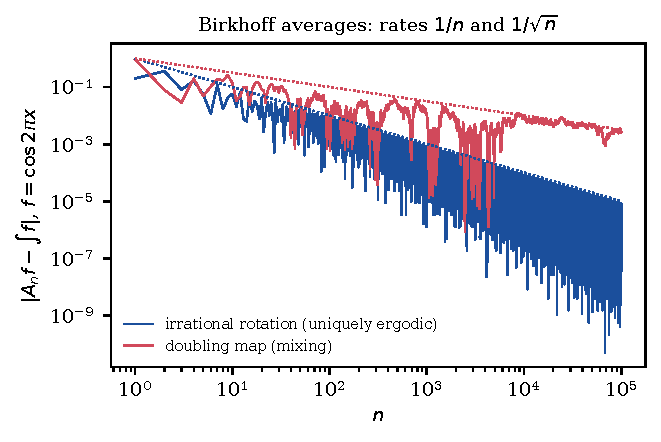
\includegraphics[width=0.85\textwidth]{birkhoff}
\caption{Birkhoff averages of $f(x)=\cos2\pi x$ along an orbit of the golden mean rotation, converging at rate $1/n$, and along an orbit of the doubling map, fluctuating at the central limit scale $1/\sqrt{n}$. The binary digits of the initial point of the doubling orbit are independent fair coin flips, and the orbit is computed as the shift of the digit sequence, each point being read from $52$ digits, because iterating $x\mapsto2x$ modulo one in floating point arithmetic reaches zero after $53$ steps. Dotted lines show the two rates.}
\label{fig:birkhoff}
\end{figure}

\section{Mixing}

\begin{definition}
A measure preserving system is mixing if $\mu(T^{-n}A\cap B)\to\mu(A)\mu(B)$ for all measurable $A,B$, equivalently $\langle U_T^nf,g\rangle\to\int f\dd\mu\int\bar g\dd\mu$ for all $f,g\in L^2$. It is weakly mixing if the convergence holds in Ces\`aro mean of absolute values.
\end{definition}

Mixing implies ergodicity: if $A$ is invariant, take $B = A$ to get $\mu(A) = \mu(A)^2$. The irrational rotation is ergodic but not mixing, since $U_T^ne_1 = e^{2\pi in\alpha}e_1$ does not tend to zero weakly.

\begin{theorem}[Koopman and von Neumann~\cite{koopmanvonneumann1932}]
\label{thm:koopman_vonneumann}
A measure preserving system is weakly mixing if and only if the Koopman operator has no eigenfunctions other than constants.
\end{theorem}

We quote the theorem without proof; see Walters~\cite{walters1982}. The rotation has eigenfunctions $e_m$ with eigenvalues $e^{2\pi im\alpha}$ and is the archetype of a system with pure point spectrum, meaning that the eigenfunctions span $L^2(\mu)$; the cat map has no eigenfunctions other than constants and is mixing.

\begin{theorem}[The cat map is mixing]
\label{thm:cat_map_mixing}
The automorphism $T(x,y) = (2x+y,x+y)$ of $\T^2$ is mixing for Lebesgue measure.
\end{theorem}

\begin{proof}
Let $A = \begin{pmatrix}2&1\\1&1\end{pmatrix}$ and, for $k\in\Z^2$, $e_k(z) = e^{2\pi ik\cdot z}$. Then $e_k\circ T = e_{A^\top k}$, so $\langle U_T^ne_k,e_l\rangle = \mathbb{1}\{(A^\top)^nk = l\}$. The matrix $A^\top = A$ has eigenvalues $\lambda^{\pm1}$ with $\lambda = \frac{3+\sqrt5}{2}$, and its stable eigenvector has irrational slope, so no nonzero integer vector lies in the stable direction. Hence for $k\neq0$ the component of $k$ along the unstable eigenvector is nonzero and $|A^nk|\to\infty$, so $\langle U_T^ne_k,e_l\rangle = 0$ for $n$ large. This proves mixing for trigonometric polynomials, and density in $L^2$ together with $\|U_T^n\| = 1$ extends it to all $f,g$.
\end{proof}

Figure~\ref{fig:cat} shows the cat map acting on a colored image discretized on a $101\times101$ grid. After a few iterations the image is mixed, as Theorem~\ref{thm:cat_map_mixing} predicts for the continuous system. But the discretized map $z\mapsto Az$ modulo $101$ is a permutation of the finite set $(\Z/101\Z)^2$, and a permutation of a finite set has finite order, which is Poincar\'e's recurrence theorem~\cite{poincare1890} in its simplest form. The image must therefore return exactly, and it does, at $n = 25$, the order of $A$ in $GL_2(\Z/101\Z)$. The figure is a picture of the Zermelo paradox~\cite{zermelo1896} of Chapter~\ref{ch:poincare}: mixing on short time scales, recurrence on long ones. The recurrence time is set by the arithmetic of the grid size $N$ and not by the number $N^2$ of cells: the period never exceeds $3N$~\cite{dysonfalk1992}. Kac's lemma (Theorem~\ref{thm:kac_lemma}) says that for an ergodic system the mean return time to a set of measure $1/N^2$ is $N^2$, and the discretized map is not ergodic. It splits the grid into cycles, here the fixed origin and $408$ cycles of length $25$, so the picture shows an artifact of the discretization and not the recurrence time of the continuous system.

\begin{figure}[t]
\centering
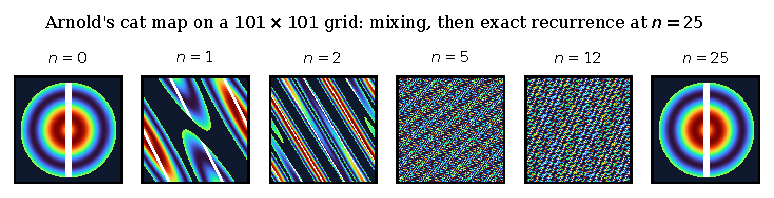
\includegraphics[width=\textwidth]{cat_map}
\caption{The cat map acting on an image on a $101\times101$ grid. The image is mixed within a few steps, and returns exactly after $25$ steps, the order of the cat map matrix modulo $101$. The discretized map is a permutation of the $101^2$ cells, and on an $N\times N$ grid its period never exceeds $3N$.}
\label{fig:cat}
\end{figure}

\section{Kolmogorov Sinai entropy}

Let $\xi = \{C_1,\dots,C_m\}$ be a finite measurable partition. Its entropy is $H(\xi) = -\sum_i\mu(C_i)\log\mu(C_i)$, and the join $\xi^n = \xi\vee T^{-1}\xi\vee\cdots\vee T^{-(n-1)}\xi$ is the partition into sets of points with the same itinerary of length $n$. By subadditivity of entropy the limit
\[
h(T,\xi) = \lim_{n\to\infty}\frac1nH(\xi^n)
\]
exists, and the Kolmogorov Sinai entropy~\cite{kolmogorov1958,sinai1959} is $h(T) = \sup_\xi h(T,\xi)$. It is an isomorphism invariant: isomorphic systems have equal entropy.

\begin{theorem}[Kolmogorov, Sinai~\cite{kolmogorov1959,sinai1959}]
\label{thm:kolmogorov_sinai}
Call a finite partition $\xi$ generating if the partitions $T^{-k}\xi$ generate $\mathcal{B}$ up to null sets, where $k$ ranges over $\Z$ if $T$ is invertible and over $k\geq0$ if it is not. If $\xi$ is generating, then $h(T) = h(T,\xi)$.
\end{theorem}

We quote the theorem without proof; see Walters~\cite[Chapter~4]{walters1982}.

\begin{example}[Entropy computations]
\begin{enumerate}
\item For the Bernoulli shift with marginal $p$, the time zero partition is generating and $\xi^n$ consists of cylinder sets with independent coordinates, so $H(\xi^n) = nH(p)$ and $h = H(p)$. Two Bernoulli shifts with different entropies are therefore not isomorphic, which answered the question of von Neumann~\cite{vonneumann1932operator} whether the shifts on two and three symbols with uniform weights are isomorphic: their entropies are $\log2$ and $\log3$.
\item For an irrational rotation, the partition into two arcs is generating, and $\xi^n$ has at most $2n$ atoms, since $n$ rotated copies of two endpoints cut the circle into at most $2n$ arcs. Hence $h\leq\lim\frac1n\log(2n) = 0$.
\item For the cat map, $h = \log\lambda = \log\frac{3+\sqrt5}{2}$, which also follows from Pesin's formula in Section~\ref{sec:lyapunov_logistic} because Lebesgue measure is invariant. More generally a toral automorphism has entropy $\sum\log|\lambda_i|$ over eigenvalues of modulus greater than one~\cite{yuzvinskii1967}; see also Walters~\cite{walters1982}.
\end{enumerate}
\end{example}

\begin{theorem}[Shannon, McMillan and Breiman~\cite{shannon1948,mcmillan1953,breiman1957}]
\label{thm:shannon_mcmillan_breiman}
Let $T$ be ergodic and $\xi$ a finite partition. Let $\xi^n(x)$ denote the atom of $\xi^n$ containing $x$. Then
\[
-\frac1n\log\mu\big(\xi^n(x)\big)\longrightarrow h(T,\xi)\qquad\text{almost surely and in }L^1.
\]
\end{theorem}

The theorem is the asymptotic equipartition property of information theory: typical itineraries of length $n$ have probability about $e^{-nh}$ and there are about $e^{nh}$ of them. We quote it without proof; see Cover and Thomas~\cite[Chapter~16]{covertomas}. For independent sequences it is the law of large numbers for $-\frac1n\sum\log p(X_i)$, and it is the dynamical form of the type counting of Chapter~\ref{ch:types}. Boltzmann's $S = k_B\log W$ and the Kolmogorov Sinai entropy, the growth rate of the number of distinguishable trajectories, are two counts of the same kind: one over configurations, the other over histories.

\begin{theorem}[Ornstein~\cite{ornstein1970}]
\label{thm:ornstein_isomorphism}
Two Bernoulli shifts on finite alphabets, indexed by $\Z$, are isomorphic if and only if they have the same entropy.
\end{theorem}

Ornstein's theorem of 1970 makes entropy a complete invariant within the Bernoulli class, and we quote it without proof. Many systems of physical interest are Bernoulli: ergodic toral automorphisms, among them the cat map~\cite{katznelson1971}, Sinai billiards~\cite{gallavottiornstein1974} and geodesic flows on surfaces of negative curvature~\cite{ornsteinweiss1973}. In these systems, at the level of measure theory, deterministic dynamics is indistinguishable from a Bernoulli shift of the same entropy.

\section{Lyapunov exponents and the logistic map}\label{sec:lyapunov_logistic}

Let $T$ be a differentiable map of an interval and $\mu$ an ergodic invariant probability measure for which $\log|T'|$ is integrable. The Lyapunov exponent is $\chi = \int\log|T'|\dd\mu$, and Birkhoff's theorem (Theorem~\ref{thm:birkhoff}) applied to $\log|T'|$ gives $\frac1n\log|(T^n)'(x)| = \frac1n\sum_{k<n}\log|T'(T^kx)|\to\chi$ for $\mu$ almost every $x$. Pesin's formula states that for a $C^2$ diffeomorphism of a compact manifold and an invariant measure absolutely continuous with respect to volume, the Kolmogorov Sinai entropy equals the integral of the sum of the positive Lyapunov exponents~\cite{pesin1977}. For absolutely continuous invariant measures of positive entropy of an interval map the corresponding statement is due to Ledrappier~\cite{ledrappier1981}. The logistic family is $T_r(x) = rx(1-x)$.

\begin{proposition}
\label{prop:logistic_r4}
For $r = 4$ the logistic map $T_4$ has the invariant density
\[
\rho(x) = \frac{1}{\pi\sqrt{x(1-x)}}
\]
on $(0,1)$. It is ergodic for $\rho$ and conjugate to the tent map, and its Lyapunov exponent and entropy with respect to $\rho$ are both $\log2$.
\end{proposition}

\begin{proof}
Let $\Lambda(y) = 1-|1-2y|$ be the tent map on $[0,1]$ and $\psi(y) = \sin^2(\pi y/2)$, an increasing homeomorphism of $[0,1]$ with $\psi'(y) = \frac\pi2\sin(\pi y)>0$ on $(0,1)$. Since $4\sin^2a\cos^2a = \sin^2(2a)$ we have $T_4(\psi(y)) = \sin^2(\pi y)$, and $\sin^2(\pi y) = \psi(\Lambda(y))$ because $\Lambda(y) = 2y$ for $y\leq\frac12$ and $\Lambda(y) = 2-2y$ for $y\geq\frac12$. Hence $T_4\circ\psi = \psi\circ\Lambda$, so $T_4$ is conjugate to the tent map. The tent map preserves Lebesgue measure, because every interval has two preimages of half its length. The image of Lebesgue measure under $\psi$ has density $\rho$, because $\psi^{-1}(x) = \frac2\pi\arcsin\sqrt x$ has derivative $\rho(x)$, so $\rho$ is invariant for $T_4$.

Let $b_1,b_2,\dots$ be the binary digits of $y$ and let $c_n = 1$ if $\Lambda^{n-1}(y)\geq\frac12$ and $c_n = 0$ otherwise. Then $c_1 = b_1$ and $c_n = b_n+b_{n-1}\pmod 2$ for $n\geq2$, because $\Lambda$ acts on a point with first digit $b_1$ by shifting the digits and, when $b_1 = 1$, complementing them. The map $(b_n)\mapsto(c_n)$ is a bijection of $\{0,1\}^{\mathbb{N}}$ that preserves the fair coin measure, since it is a bijection of $\{0,1\}^n$ on the first $n$ coordinates for every $n$. For Lebesgue distributed $y$ the digits $b_n$ are fair coin flips, so the itinerary $(c_n)$ of $y$ with respect to $[0,\frac12]$ and $[\frac12,1]$ is a sequence of fair coin flips, and $\Lambda$ acts on itineraries as the shift. Thus $\Lambda$ is isomorphic to the one sided fair coin shift. It follows that $\Lambda$ is ergodic for Lebesgue measure and $T_4$ is ergodic for $\rho$. The itinerary determines $y$, so the partition at $\frac12$ is a one sided generator with $H(\xi^n) = n\log2$, and Theorem~\ref{thm:kolmogorov_sinai} gives $h(\Lambda) = \log2$. Isomorphic systems have equal entropy, so $T_4$ has entropy $\log2$ for $\rho$.

For the exponent, differentiate $T_4\circ\psi = \psi\circ\Lambda$ at $y\neq\frac12$, using $|\Lambda'| = 2$, to get
\[
\log|T_4'(\psi(y))| = \log2+\ell(\Lambda(y))-\ell(y),
\]
where $\ell(y) = \log\psi'(y) = \log\frac\pi2+\log\sin(\pi y)$. The function $\ell$ is integrable on $[0,1]$, since $\log\sin(\pi y)$ has only logarithmic singularities at the endpoints. Integrate over $y$ with respect to Lebesgue measure. Because $\Lambda$ preserves it, $\int\ell\circ\Lambda\dd y = \int\ell\dd y$, and because $\psi$ carries it to $\rho(x)\dd x$ we obtain $\int\log|T_4'|\rho\dd x = \log2$. So $\log|T_4'|$ is integrable for $\rho$, although $T_4'$ vanishes at $x = \frac12$, and $\chi = \log2$. The entropy equals $\chi$, in agreement with the entropy formula for interval maps.
\end{proof}

The invariant density is the arcsine law, the Beta$(\frac12,\frac12)$ distribution. It is L\'evy's law of the time that Brownian motion spends positive (Chapter~\ref{ch:brownian}) and the law of the horseshoe shrinkage coefficient (Chapter~\ref{ch:mixtures}). Ulam and von Neumann proposed iterating this map as a generator of random numbers~\cite{ulamvonneumann1947}. Figure~\ref{fig:logistic} shows the attractor of the logistic family as $r$ varies, colored by the numerically computed Lyapunov exponent. Periodic windows, where the exponent is negative and the attractor is a finite cycle, alternate with chaotic parameter sets of positive Lebesgue measure, a theorem of Jakobson~\cite{jakobson1981}; Lyubich proved that for almost every parameter the map is either regular or stochastic~\cite{lyubich2002}.

\begin{figure}[t]
\centering
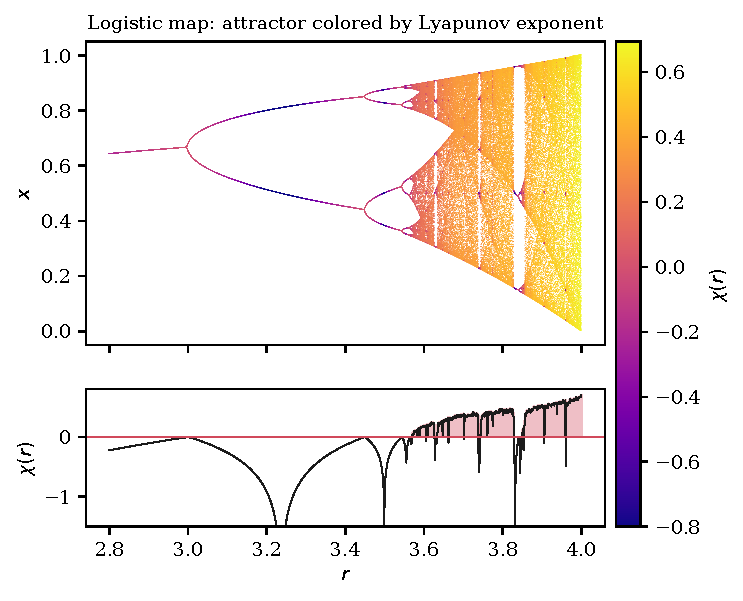
\includegraphics[width=0.85\textwidth]{logistic}
\caption{The logistic map $x\mapsto rx(1-x)$ for $1600$ values of $r$ from $2.8$ to $4$. Top, the attractor, drawn from the last $150$ of $400$ iterates that follow $600$ discarded ones, colored by the Lyapunov exponent with the color scale clipped to the interval from $-0.8$ to $0.7$. Bottom, the exponent, estimated as the average of $\log|r(1-2x_k)|$ over the $400$ iterates, positive (shaded) on chaotic parameters and negative in periodic windows; the vertical axis is cut at $-1.5$.}
\label{fig:logistic}
\end{figure}

\section{KAM theory and the failure of ergodicity}

Kolmogorov announced in 1954~\cite{kolmogorov1954}, and Arnold~\cite{arnold1963} and Moser~\cite{moser1962} proved in the early 1960s, that for a small perturbation of an integrable Hamiltonian system satisfying a nondegeneracy condition, most invariant tori survive, deformed but intact, and fill a set of positive measure. On each surviving torus the motion is quasiperiodic, and the energy surface is not ergodic. Markus and Meyer showed in 1974~\cite{markusmeyer1974} that generic Hamiltonian systems are neither integrable nor ergodic. The standard map of Chirikov~\cite{chirikov1979}
\[
p_{n+1} = p_n+K\sin q_n,\qquad q_{n+1} = q_n+p_{n+1}\pmod{2\pi}
\]
is the simplest model. Figure~\ref{fig:standard} shows orbits at the parameter at which, according to Greene's criterion~\cite{greene1979}, the last invariant circle spanning the cylinder breaks. Invariant curves, chains of islands around periodic orbits, and a chaotic sea coexist, as they do in the H\'enon Heiles system of Figure~\ref{fig:hh}. Ergodicity fails for typical Hamiltonian systems with few degrees of freedom, and Boltzmann's hypothesis cannot be the foundation of statistical mechanics for them.

\begin{figure}[t]
\centering
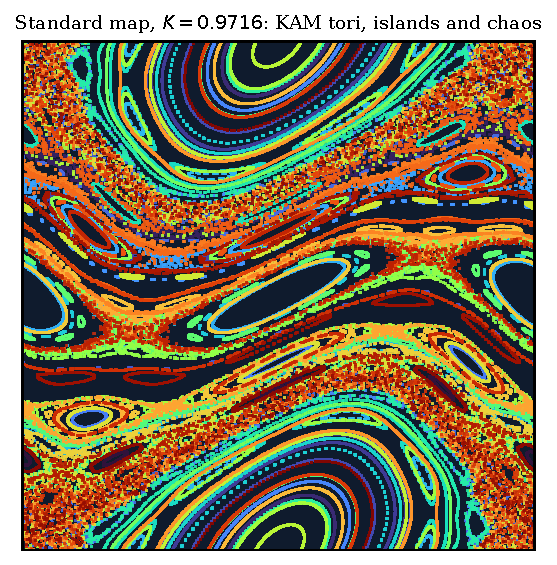
\includegraphics[width=0.78\textwidth]{standard_map}
\caption{Ninety orbits of the Chirikov standard map at $K = 0.971635$, near the breakup of the last spanning invariant circle, each in its own color: invariant curves, island chains and a chaotic sea. Each orbit has $900$ points, and the initial points are drawn uniformly from $[0,2\pi)^2$ with a fixed random seed.}
\label{fig:standard}
\end{figure}

\section{Khinchin's argument}

Khinchin's \emph{Mathematical Foundations of Statistical Mechanics}, published in Russian in 1943 and in English in 1949~\cite{khinchin1949}, replaced ergodicity by concentration. Consider $n$ particles with phase point $z = (z_1,\dots,z_n)$ on an energy surface, a Hamiltonian $H(z) = \sum_iH_i(z_i)$ that is a sum of one particle terms, and a sum function $F(z) = \sum_if_i(z_i)$, the form of macroscopic observables such as pressure or kinetic energy, with summands $f_i$ bounded independently of $n$ and a microcanonical mean $m$ of order $n$. Khinchin showed that the standard deviation $s$ of $F$ for the microcanonical measure is of order $n^{1/2}$. Markov's inequality gives $\P(|F-m|\geq am)\leq s/(am)$, which is of order $n^{-1/2}/a$, so the set where the relative deviation of $F$ exceeds $k_1n^{-1/4}$ has microcanonical measure at most $k_2n^{-1/4}$, with $k_1$ and $k_2$ independent of $n$. The mean ergodic theorem, which needs no ergodicity, carries the bound over to time averages. Let $T$ be the time one map of the Hamiltonian flow, which preserves the microcanonical measure. By Theorem~\ref{thm:vonneumann} the averages $\frac1N\sum_{k<N}F\circ T^k$ converge in $L^2$, as $N\to\infty$ at fixed $n$, to $\E[F\mid\mathcal{I}]$, the conditional expectation given the invariant $\sigma$ algebra. This limit has the same mean as $F$ and a variance no larger than that of $F$, because conditional expectation is an orthogonal projection in $L^2$, so Markov's inequality gives it the same bound. Hence, whatever the ergodic properties of the dynamics, the infinite time average of $F$ differs from its phase average by less than the fraction $k_1n^{-1/4}$ of the phase average except on a set of initial conditions of measure at most $k_2n^{-1/4}$. This is Khinchin's theorem, which Mazur and van der Linden extended to particles with short range interactions~\cite{mazurvanderlinden1963}. The argument is the one we use in Chapter~\ref{ch:entropy} to explain why macroscopic observables are deterministic: Lipschitz functions of many weakly dependent coordinates concentrate. In this sense the sixth problem needs less than ergodicity and more than it: less, because concentration suffices for equilibrium averages; more, because the approach to equilibrium on physical time scales is a statement about the dynamics of the one particle law, the subject of Lanford's theorem~\cite{lanford1975} in Chapter~\ref{ch:kinetic}, and not about infinite time averages.

\section{The ergodic decomposition and de Finetti}

The set of $T$ invariant probability measures is convex and, for a continuous map of a compact metric space, weakly compact. Its extreme points are exactly the ergodic measures: if $\mu = t\mu_1+(1-t)\mu_2$ nontrivially and $A$ is invariant with $0<\mu(A)<1$, then $\mu(\cdot\mid A)$ and $\mu(\cdot\mid A^c)$ give such a decomposition, and conversely. This set is moreover a Choquet simplex, a compact convex set in which every point is the barycenter of a unique probability measure on the extreme points~\cite{phelps2001}, so Choquet theory gives the ergodic decomposition: every invariant measure is a unique mixture of ergodic ones,
\[
\mu = \int\mu_\theta\,\Pi(\dd\theta),
\]
where $\theta$ labels the ergodic measures and $\mu_\theta$ is the conditional measure of $\mu$ given the invariant $\sigma$ algebra, obtained by disintegration; see Walters~\cite{walters1982}. De Finetti's theorem (Theorem~\ref{thm:definetti}) is the ergodic decomposition for the group of finite permutations acting on sequences: the invariant measures are exchangeable laws, the ergodic ones are, by the Hewitt Savage zero one law~\cite{hewittsavage1955}, the independent identically distributed laws, and the mixing measure $\Pi$ is the prior; see Kallenberg~\cite{kallenberg2005}. Birkhoff's theorem says that the empirical frequencies along a single orbit identify the ergodic component, so that the parameter $\theta$ is a function of the whole sequence, and the martingale convergence theorem then gives $\E[g(\theta)\mid X_1,\dots,X_n]\to g(\theta)$ almost surely for bounded $g$. This is the statement that the posterior concentrates on the true parameter, Doob's theorem~\cite{doob1949} (Theorem~\ref{thm:doob}) seen through the ergodic decomposition.

\section{Markov chains, spectral gaps and Monte Carlo}\label{sec:markov_spectral_mc}

A Markov kernel $P$ is reversible with respect to $\pi$ if $\pi(\dd x)P(x,\dd y) = \pi(\dd y)P(y,\dd x)$, and then $\pi$ is invariant for $P$. The stationary chain is a stationary process, and if the chain is irreducible, meaning that every $P$ invariant set has $\pi$ measure zero or one, the shift on path space is ergodic. Birkhoff's theorem (Theorem~\ref{thm:birkhoff}) applied to the shift gives $\frac1n\sum_{k<n}f(X_k)\to\int f\dd\pi$ almost surely for $f\in L^1(\pi)$ and $\pi$ almost every starting point. Its quantitative form is a central limit theorem.

\begin{theorem}[Kipnis and Varadhan~\cite{kipnisvaradhan1986}]
\label{thm:kipnis_varadhan}
Let $P$ be reversible with respect to $\pi$ and aperiodic, with spectrum in $[-1,1-g]$ on mean zero functions, $g>0$. For $f\in L^2(\pi)$ with $\int f\dd\pi = 0$, the stationary chain satisfies $\frac{1}{\sqrt n}\sum_{k<n}f(X_k)\to N(0,\sigma_f^2)$ in law, with
\[
\sigma_f^2 = \big\langle f,(I+P)(I-P)^{-1}f\big\rangle_\pi\leq\frac{2-g}{g}\,\Var_\pi(f).
\]
\end{theorem}

We quote the central limit theorem without proof; see Roberts and Rosenthal~\cite{robertsrosenthal2004} for the statement for chains in discrete time.

\begin{proof}[Proof of the variance bound]
By the spectral theorem, $\sigma_f^2 = \int\frac{1+s}{1-s}\,\nu_f(\dd s)$ where $\nu_f$ is the spectral measure of $f$, supported in $[-1,1-g]$ with total mass $\Var_\pi(f)$. The function $s\mapsto\frac{1+s}{1-s}$ is increasing, so it is at most $\frac{2-g}{g}$ on the support.
\end{proof}

The spectral gap $g$ is a Poincar\'e constant in the sense of Chapter~\ref{ch:poincare}, and the asymptotic variance of a Monte Carlo average is the integrated autocorrelation of the chain. Every Markov chain Monte Carlo computation in this book, from the Gibbs samplers of P\'olya Gamma augmentation in Chapter~\ref{ch:mixtures} to the preconditioned Crank Nicolson sampler for Navier Stokes posteriors in Chapter~\ref{ch:nsinference}, is an application of the ergodic theorem, and for the reversible samplers among them the cost is governed by a spectral gap. The preconditioned Crank Nicolson proposal is reversible with respect to the Gaussian prior, so the Metropolis accept step makes the chain reversible with respect to the posterior~\cite{cotter2013}. A Gibbs sampler that alternates between two blocks $u$ and $v$ is not reversible as a chain on the pair, but its marginal chain on $u$ is: with $K(u,\dd u') = \int p(\dd v\mid u)\,p(\dd u'\mid v)$ and $\pi$ the marginal law of $u$, we have $\pi(\dd u)K(u,\dd u') = \int p(\dd v)\,p(\dd u\mid v)\,p(\dd u'\mid v)$, which is symmetric in $u$ and $u'$. The physicists of Los Alamos who invented the Metropolis algorithm~\cite{metropolis1953} were, in this precise sense, building an ergodic system on purpose.

\section*{Notes}

Walters's \emph{Introduction to Ergodic Theory}~\cite{walters1982} and Petersen's \emph{Ergodic Theory}~\cite{petersen1983} cover the material of this chapter, and Arnold and Avez~\cite{arnoldavez1968} treat the cat map and the other classical examples. The ergodic decomposition view of de Finetti's theorem is developed by Kallenberg in \emph{Probabilistic Symmetries and Invariance Principles}~\cite{kallenberg2005}.

\section*{Exercises}
\begin{enumerate}
\item Show that the doubling map is mixing by computing $\langle U_T^ne_k,e_l\rangle$.
\item Let $T$ be the cat map and $\lambda = \frac{3+\sqrt5}{2}$. Show that $T^n$ has exactly $\lambda^n+\lambda^{-n}-2$ fixed points on $\T^2$, and that their exponential growth rate is the entropy $h(T)$.
\item For the doubling map $T$ and $f(x) = \cos2\pi x$, show that the functions $f\circ T^k$, $k\geq0$, are orthogonal in $L^2$ and that $\E[f\mid T^{-1}\mathcal{B}] = 0$. Deduce that the Birkhoff average $A_nf$ has variance exactly $1/(2n)$, and that $\sqrt nA_nf$ converges in law to $N(0,\frac12)$ by the martingale central limit theorem.
\item For the golden mean $\alpha$, show that $|\sin\pi m\alpha|\geq c/m$ for some $c>0$ and all $m\geq1$. Deduce that for the rotation by $\alpha$ the Birkhoff averages of every $f$ with $\sum_m|m||\hat f(m)|<\infty$ converge to $\int f$ at the rate $O(1/n)$.
\item Let $P$ be the transition matrix of the chain on $\{-1,+1\}$ that changes state with probability $p\in(0,1)$. For $f(x) = x$, compute the spectral gap and the asymptotic variance of $\frac{1}{\sqrt n}\sum_{k<n}f(X_k)$, and decide whether the bound of Theorem~\ref{thm:kipnis_varadhan} is attained.
\item Show that the period of the cat map on an $N\times N$ grid equals the order of $A$ in $GL_2(\Z/N\Z)$, and compute it for $N = 101$. Compare the cycle lengths with the mean return time that Kac's lemma (Theorem~\ref{thm:kac_lemma}) gives for an ergodic system on $N^2$ cells.
\end{enumerate}

\chapter{The Method of Types and Moment Conditioning}
\label{ch:types}

\section{Counting as a theory of probability}

Boltzmann's derivation of 1877~\cite{boltzmann1877} counted the ways of distributing molecules among cells of phase space. Eighty years later Sanov~\cite{sanov1957} proved the large deviation theorem for empirical distributions, and Csisz\'ar and K\"orner~\cite{csiszarkorner2011} made the counting into a systematic method, the method of types, which gives exact, nonasymptotic bounds for the probabilities of empirical distributions on finite alphabets. The method is elementary. It proves Sanov's theorem, the conditional limit theorem and Stein's lemma on finite alphabets, and it explains why conditioning a large system on its macroscopic moments produces the exponential families of statistical mechanics.

\section{Types and type classes}

Let $\mathcal{X} = \{1,\dots,m\}$ and $x = (x_1,\dots,x_n)\in\mathcal{X}^n$. The type of $x$ is its empirical distribution $Q_x(a) = \frac1n\#\{i:x_i = a\}$. Let $\mathcal{P}_n$ be the set of types of sequences of length $n$, and for $Q\in\mathcal{P}_n$ let $T(Q) = \{x:Q_x = Q\}$ be its type class. For independent random variables $X_1,X_2,\dots$ with values in $\mathcal{X}$, write $L_n$ for the type of $(X_1,\dots,X_n)$, the empirical measure. Logarithms are natural, $H(Q) = -\sum_aQ(a)\log Q(a)$ is the Shannon entropy, and $\KL(Q\|P) = \sum_aQ(a)\log\frac{Q(a)}{P(a)}$ is the relative entropy, with $0\log0 = 0$ and $\KL(Q\|P) = \infty$ unless $Q$ vanishes wherever $P$ does.

\begin{theorem}[Type counting]
\label{thm:typecount}
\begin{enumerate}
\item $|\mathcal{P}_n|\leq(n+1)^m$.
\item For any law $P$ on $\mathcal{X}$ and $x\in T(Q)$, $P^n(x) = \exp\big(-n(H(Q)+\KL(Q\|P))\big)$.
\item For $Q\in\mathcal{P}_n$, $(n+1)^{-m}e^{nH(Q)}\leq|T(Q)|\leq e^{nH(Q)}$.
\item For $Q\in\mathcal{P}_n$ and any $P$, $(n+1)^{-m}e^{-n\KL(Q\|P)}\leq P^n(T(Q))\leq e^{-n\KL(Q\|P)}$.
\end{enumerate}
\end{theorem}

\begin{proof}
(1) Each coordinate $nQ(a)$ takes one of $n+1$ values. (2) $P^n(x) = \prod_aP(a)^{nQ(a)} = \exp(n\sum_aQ(a)\log P(a))$, and $\sum_aQ\log P = -H(Q)-\KL(Q\|P)$. (3) By (2) with $P = Q$, every sequence in $T(Q)$ has $Q^n$ probability $e^{-nH(Q)}$, so $1\geq Q^n(T(Q)) = |T(Q)|e^{-nH(Q)}$. For the lower bound we show that $T(Q)$ is the most probable type class under $Q^n$: for $Q'\in\mathcal{P}_n$,
\[
\begin{aligned}\frac{Q^n(T(Q))}{Q^n(T(Q'))} &= \prod_a\frac{(nQ'(a))!}{(nQ(a))!}\,Q(a)^{n(Q(a)-Q'(a))}\\ &\geq\prod_a(nQ(a))^{n(Q'(a)-Q(a))}Q(a)^{n(Q(a)-Q'(a))} = 1,\end{aligned}
\]
using $k!/l!\geq l^{k-l}$ and $\sum_aQ'(a) = \sum_aQ(a)$. Since there are at most $(n+1)^m$ types, $Q^n(T(Q))\geq(n+1)^{-m}$, and $|T(Q)| = Q^n(T(Q))e^{nH(Q)}$. (4) Multiply (3) by the common probability $e^{-n(H(Q)+\KL(Q\|P))}$ from (2).
\end{proof}

Part (3) is Boltzmann's $\log W = nH$ with a polynomial correction, and part (4) is the exact form of Sanov's theorem~\cite{sanov1957} (Theorem~\ref{thm:sanov}): the probability of observing the type $Q$ when the truth is $P$ decays at the rate $\KL(Q\|P)$, with no error term beyond a polynomial factor. The bounds are those of Csisz\'ar and K\"orner~\cite{csiszarkorner2011} and of Cover and Thomas~\cite[Section~11.1]{covertomas}.

Figure~\ref{fig:types} shows the types as points of the probability simplex, superimposed on the contours of $\KL(Q\|P)$. Types near $P$ are exponentially more likely than distant ones, and the rate is read off the contour on which a type lies.

\begin{figure}[t]
\centering
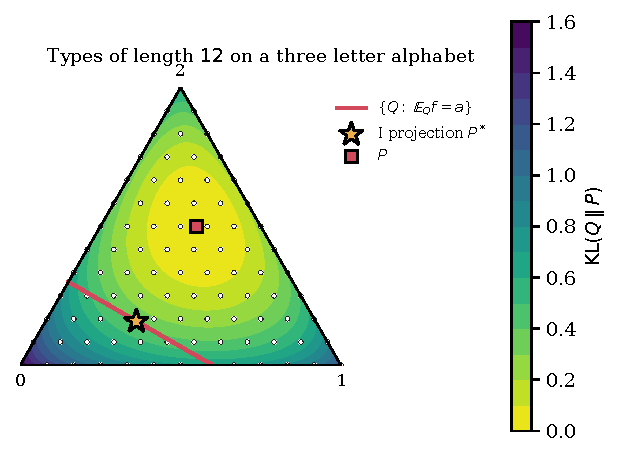
\includegraphics[width=0.78\textwidth]{types_simplex}
\caption{Types of length $12$ on $\{0,1,2\}$ (the $91$ white points, the lattice points of the simplex with spacing $1/12$) over the contours of $\KL(Q\,\|\,P)$ with $P=(0.2,0.3,0.5)$ (square). The corners of the triangle are the point masses at $0$ (lower left), $1$ (lower right) and $2$ (top). The straight line is the linear family $\{Q:\E_Qf=0.6\}$ for $f(x)=x$, and the star is its I projection $P^*\approx(0.559,0.283,0.159)$, an exponential tilt of $P$. No type of length $12$ lies on the line, because $12\,\E_Qf = 7.2$ is not an integer, so the line passes between the points.}
\label{fig:types}
\end{figure}

\section{The I projection and the Pythagorean theorem}

\begin{definition}
Let $E$ be a closed convex set of laws on $\mathcal{X}$ and $P$ a law with full support such that $\KL(Q\|P)<\infty$ for some $Q\in E$. The I projection of $P$ onto $E$ is the unique $P^*\in E$ minimizing $\KL(Q\|P)$ over $E$.
\end{definition}

Existence follows from compactness and lower semicontinuity, uniqueness from strict convexity of $Q\mapsto\KL(Q\|P)$.

\begin{theorem}[Csisz\'ar's Pythagorean inequality]
\label{thm:pythagoras}
Let $P^*$ be the I projection of $P$ onto the closed convex set $E$. Then for every $Q\in E$,
\[
\KL(Q\,\|\,P)\geq\KL(Q\,\|\,P^*)+\KL(P^*\,\|\,P).
\]
If $E$ is a linear family $\{Q:\E_Qf_j = a_j,\ j = 1,\dots,r\}$, equality holds for every $Q\in E$. If in addition $P^*$ has full support, $P^*$ is the exponential tilt
\[
P^*(x) = \frac{P(x)\exp\big(\sum_j\lambda_jf_j(x)\big)}{Z(\lambda)},
\]
with $\lambda$ chosen so that the moment constraints hold.
\end{theorem}

\begin{proof}
For $Q\in E$ and $t\in[0,1]$, $Q_t = (1-t)P^*+tQ\in E$, so $\phi(t) = \KL(Q_t\|P)$ is minimized at $t = 0$. First, $Q\ll P^*$. If $Q(x_0)>0 = P^*(x_0)$ for some $x_0$, the term $Q_t(x_0)\log\frac{Q_t(x_0)}{P(x_0)}$ of $\phi$ has a derivative that tends to $-\infty$ as $t\downarrow0$, while the derivative of every other term is bounded above near $0$, so that $\phi(t)<\phi(0)$ for small $t>0$, a contradiction. All sums below therefore run over the support of $P^*$, and the right derivative of $\phi$ at $0$ is nonnegative:
\[
\phi'(0^+) = \sum_x\big(Q(x)-P^*(x)\big)\log\frac{P^*(x)}{P(x)}\geq0,
\]
where the constant produced by differentiating $q\log q$ drops out because $\sum_x(Q(x)-P^*(x)) = 0$. A direct computation shows that
\[
\begin{aligned}\KL(Q\|P)-\KL(Q\|P^*)-\KL(P^*\|P) &= \sum_xQ\log\frac{P^*}{P}-\sum_xP^*\log\frac{P^*}{P}\\ &= \phi'(0^+),\end{aligned}
\]
which proves the inequality. For a linear family, $Q_t\in E$ also for small negative $t$, because the constraints are affine in $t$ and $Q_t\geq0$ since $Q\ll P^*$. Then $\phi$ is differentiable at $0$ and minimized there, so $\phi'(0) = 0$ and equality holds. Now let $P^*$ have full support. Then $P^*+t\nu\in E$ for small $|t|$ and every signed measure $\nu$ with total mass zero and $\sum_x\nu(x)f_j(x) = 0$ for all $j$, and the same argument gives $\sum_x\nu(x)\log\frac{P^*(x)}{P(x)} = 0$. So $\log(P^*/P)$ is orthogonal to all such $\nu$, hence lies in the span of $1,f_1,\dots,f_r$, which is the exponential form.
\end{proof}

The theorem is due to Csisz\'ar~\cite[Theorem~2.2]{csiszar1975}, who also proved the exponential form~\cite[Theorem~3.1]{csiszar1975}. It says that relative entropy behaves like squared Euclidean distance, with exponential families playing the role of orthogonal complements of linear families. Two consequences are used repeatedly. First, maximum likelihood in the exponential family $\{P_\lambda\}$ and I projection onto the linear family of laws with the observed moments are dual problems with the same solution: a maximizer of the log likelihood per observation, $\sum_j\lambda_ja_j-\log Z(\lambda)$ plus a constant, where $a_j$ is the observed mean of $f_j$, satisfies $\E_{P_\lambda}f_j = a_j$, so $P_\lambda$ lies in the linear family, and a tilt that lies in the linear family is its I projection~\cite[Theorem~3.1]{csiszar1975}. This duality makes the maximum entropy principle~\cite{jaynes1957} and maximum likelihood two faces of one computation. Second, iterative proportional fitting~\cite{demingstephan1940} and Sinkhorn's algorithm~\cite{sinkhorn1964} of Chapter~\ref{ch:gbc} are alternating I projections onto two linear families, the laws on a product alphabet with a given first marginal $r$ and those with a given second marginal $c$. Start from a law $\pi_0 = P$ with full support, and let $\pi_{t+1}$ be the I projection of $\pi_t$ onto the first family when $t$ is even and onto the second when $t$ is odd; the I projection onto a marginal constraint rescales the rows, or the columns, of $\pi_t$. The two families intersect, since both contain $r\otimes c$, and Csisz\'ar~\cite[Theorem~3.2]{csiszar1975} showed that $\pi_t$ then converges to the I projection $\pi^*$ of $P$ onto the intersection. Because $\pi^*$ lies in both families, the Pythagorean identity gives $\KL(\pi^*\|\pi_t) = \KL(\pi^*\|\pi_{t+1})+\KL(\pi_{t+1}\|\pi_t)$ at every step, so that relative entropy to $\pi^*$ descends monotonically (Exercise~\ref{ex:ipf}). Chapter~\ref{ch:gbc} proves the convergence of Sinkhorn's algorithm by another route, Birkhoff's contraction in Hilbert's projective metric.

\section{The conditional limit theorem}

\begin{theorem}[Conditional limit theorem]
\label{thm:conditional}
Let $X_1,X_2,\dots$ be independent with law $P$ of full support on $\mathcal{X}$ and let $E$ be a closed convex set of laws with I projection $P^*$. Suppose that for all large $n$ the set $E$ contains a type $Q_n\in\mathcal{P}_n$, and that $Q_n\to P^*$. Then $\P(L_n\in E)>0$ for all large $n$, and for every fixed $k$,
\[
\mathrm{Law}\big(X_1,\dots,X_k\,\big|\,L_n\in E\big)\longrightarrow(P^*)^{\otimes k}.
\]
Moreover $\P(\KL(L_n\|P^*)>\delta\mid L_n\in E)\to0$ exponentially fast for each $\delta>0$.
\end{theorem}

\begin{proof}
By the Pythagorean inequality of Theorem~\ref{thm:pythagoras}, every type $Q\in E$ with $\KL(Q\|P^*)>\delta$ has $\KL(Q\|P)\geq\KL(P^*\|P)+\delta$. By Theorem~\ref{thm:typecount}, the total probability of such types is at most $(n+1)^me^{-n(\KL(P^*\|P)+\delta)}$. Since $Q_n\to P^*$ and $P$ has full support, $\KL(Q_n\|P)\to\KL(P^*\|P)$, and hence $\P(L_n\in E)\geq\P(L_n = Q_n)\geq(n+1)^{-m}e^{-n(\KL(P^*\|P)+\delta/2)}$ for large $n$. The ratio is at most $(n+1)^{2m}e^{-n\delta/2}$, which is the second claim. For the first, let $Q\in E\cap\mathcal{P}_n$. Conditionally on $L_n = Q$ the sequence is uniform on the type class, so the law of $(X_1,\dots,X_k)$ is that of sampling without replacement from an urn with composition $nQ$. Sampling with replacement gives $Q^{\otimes k}$, and the two laws differ by at most the probability that $k$ draws with replacement from $n$ balls include a repeat, which is at most $k(k-1)/(2n)$. This is the bound of Diaconis and Freedman~\cite{diaconisfreedman1980}, with total variation taken as the supremum over events. Total variation is subadditive for products, so $Q^{\otimes k}$ is within $k\,\mathrm{TV}(Q,P^*)$ of $(P^*)^{\otimes k}$, and Pinsker's inequality~\cite[Lemma~11.6.1]{covertomas} gives $\mathrm{TV}(Q,P^*)\leq\sqrt{\KL(Q\|P^*)/2}$. Averaging over the conditional law of the type, the law of $(X_1,\dots,X_k)$ given $L_n\in E$ is within $k(k-1)/(2n)+k\sqrt{\delta/2}+(n+1)^{2m}e^{-n\delta/2}$ of $(P^*)^{\otimes k}$ in total variation, for every $\delta>0$, and the claim follows by letting $n\to\infty$ and then $\delta\downarrow0$.
\end{proof}

This is the conditional limit theorem of Van Campenhout and Cover~\cite{vancampenhoutcover1981} and Csisz\'ar~\cite{csiszar1984}, proved by types as in Cover and Thomas~\cite[Section~11.6]{covertomas}. Theorem~\ref{thm:gibbs_conditioning} proves Gibbs conditioning for one inequality constraint on the mean of a single function. The theorem above allows any closed convex set of laws, such as several moment constraints at once, and its proof gives explicit bounds: an exponential rate for the concentration of the type and the error $k(k-1)/(2n)$ from the urn. The proof makes visible why the limit is an exponential tilt: conditioning on a macroscopic constraint selects the most probable type compatible with it, and the most probable type is the I projection, which is a tilt when the constraint is linear by Theorem~\ref{thm:pythagoras}. The urn step is de Finetti's theorem for finite sequences~\cite{diaconisfreedman1980} (Theorem~\ref{thm:diaconis_freedman}): conditionally on its type, a sequence is exchangeable and its short marginals are nearly independent.

The hypothesis on $E$ holds whenever $E$ has nonempty interior in the simplex: a ball around an interior point contains a type for every large $n$, and every point of a convex set with interior, in particular $P^*$, is a limit of interior points. This covers the inequality constraints $\{Q:\E_Q\varepsilon\leq a\}$ of Theorem~\ref{thm:gibbs_conditioning} and shells $\{a\leq\E_Qf\leq a+\delta\}$ of positive width. It also holds for an equality constraint $\{Q:\E_Qf = a\}$ when $f$ is integer valued and $P^*$ has full support, along the $n$ for which $E$ contains a type at all: the count vectors of types in $E$ are the integer points of an affine subspace that contains $nP^*$, they form a translate of a lattice, and so one of them lies within a bounded distance of $nP^*$. The proof then gives the conclusion along those $n$. For a real valued $f$ no type lies in $\{Q:\E_Qf = a\}$ in general, and the conditional laws are computed exactly, as in the next section.

\section{Moment conditioning: exact computations}

The conditional limit theorem holds far beyond finite alphabets, as Csisz\'ar showed~\cite{csiszar1984}, and in several classical cases the conditional law can be computed exactly for every $n$.

\begin{proposition}[Exponential samples]
\label{prop:expsamples}
Let $X_1,\dots,X_n$ be independent standard exponential variables and $a>0$. Conditionally on $\bar X_n = a$, the law of $X_1$ has density
\[
p_n(x) = \frac{n-1}{na}\Big(1-\frac{x}{na}\Big)^{n-2},\qquad0<x<na,
\]
which converges as $n\to\infty$ to the exponential density with mean $a$, the exponential tilt of the standard exponential law that has mean $a$. The total variation distance to this limit does not depend on $a$ and equals $c/n+O(n^{-2})$, where $c = (1+\sqrt2)e^{-(2+\sqrt2)}+(\sqrt2-1)e^{-(2-\sqrt2)}\approx0.3100$.
\end{proposition}

\begin{proof}
The joint density $e^{-\sum_ix_i}$ of $(X_1,\dots,X_n)$ depends on $x$ only through $\sum_ix_i$, so given $\sum_iX_i = na$ the vector is uniform on the simplex $\{x_i\geq0,\ \sum_ix_i = na\}$. The slice of this simplex at $x_1 = x$ is a simplex of dimension $n-2$ and side $na-x$, whose volume is proportional to $(na-x)^{n-2}$, and normalizing gives $p_n$. The pointwise limit follows from $(1-x/na)^{n-2}\to e^{-x/a}$, and Scheff\'e's lemma upgrades it to total variation. The tilt $P_\lambda(\dd x)\propto e^{\lambda x}e^{-x}\dd x$ with mean $a$ is the exponential law with rate $1-\lambda = 1/a$. For the rate, put $u = x/a$, so that $a\,p_n(x) = g_n(u) = (1-\frac1n)(1-\frac un)^{n-2}$ for $0<u<n$ and the tilt has density $e^{-u}$ in $u$. The total variation distance is $\frac12\int|g_n(u)-e^{-u}|\dd u$, which does not depend on $a$. Expanding the logarithm of $e^ug_n(u)$ gives, for $n\geq4$ and uniformly in $0<u\leq n/2$, $g_n(u) = e^{-u}\big(1+h(u)/n+R_n(u)\big)$ with $h(u) = 2u-\frac12u^2-1$ and $|R_n(u)|\leq C(1+u^4)/n^2$, while both laws give probability $O(e^{-n/2})$ to $u>n/2$. Hence the distance is $c/n+O(n^{-2})$ with $c = \frac12\int_0^\infty e^{-u}|h(u)|\dd u$. The polynomial $h$ is positive exactly between its roots $2\pm\sqrt2$, and $\int_0^\infty e^{-u}h(u)\dd u = 0$, so that $c = \int_{2-\sqrt2}^{2+\sqrt2}e^{-u}h(u)\dd u$. An antiderivative of $e^{-u}h(u)$ is $e^{-u}(\frac12u^2-u)$, which gives the stated value. The rate $1/n$ agrees with the bound $(k+1)/(n-k-1)$ of Diaconis and Freedman~\cite{diaconisfreedman1987} for the first $k$ coordinates of a uniform point on a simplex, with total variation taken as the supremum over events.
\end{proof}

Figure~\ref{fig:conditioning} shows $p_n$ and the total variation distance on logarithmic axes. The slope is minus one: the conditioned law converges at rate $1/n$.

\begin{figure}[t]
\centering
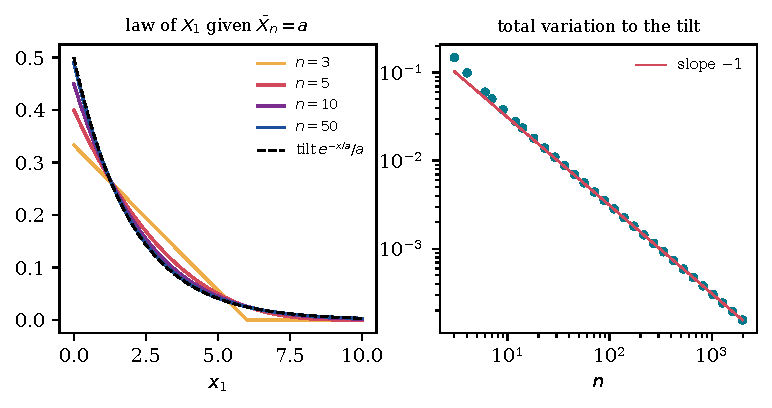
\includegraphics[width=\textwidth]{conditioning}
\caption{Moment conditioning. Left, the law of $X_1$ given $\bar X_n=2$ for independent standard exponentials, for $n=3,5,10,50$, with the exponential tilt (dashed). Right, the total variation distance to the tilt, which is the same for every mean, decays like $1/n$ with constant $c\approx0.31$.}
\label{fig:conditioning}
\end{figure}

\begin{proposition}[Poisson samples]
\label{prop:poisson}
Let $X_1,\dots,X_n$ be independent Poisson variables with mean one. Conditionally on $\sum_iX_i = N$, the vector is multinomial with $N$ trials and equal cell probabilities, so $X_1$ is Binomial$(N,1/n)$. If $N/n\to a$, this converges to the Poisson law with mean $a$, which is the exponential tilt $P_\lambda(x)\propto e^{\lambda x}\frac{e^{-1}}{x!}$ with $e^\lambda = a$.
\end{proposition}

\begin{proof}
The multinomial statement is the standard Poisson splitting identity read backwards, and the binomial to Poisson limit is classical.
\end{proof}

\section{Conditioning on collision invariants}

The equilibria of the Boltzmann equation are the Maxwellians, the densities whose logarithms are collision invariants, by the $H$ theorem (Theorem~\ref{thm:htheorem} of Chapter~\ref{ch:kinetic}). Moment conditioning gives them a second characterization: they are the laws of a single particle in a large system conditioned on its total mass, momentum and energy. Example~\ref{ex:maxwellian} of Chapter~\ref{ch:axioms} conditions on the energy alone; here the momentum is fixed as well, and the statement for $k$ particles comes with a rate.

\begin{theorem}[Moment conditioning produces Maxwellians]
\label{thm:maxwellian}
Let $V_1,\dots,V_n$ be independent standard Gaussian vectors in $\R^d$, and condition on
\[
\frac1n\sum_{i=1}^nV_i = u,\qquad\frac1n\sum_{i=1}^n|V_i-u|^2 = d\theta,
\]
with $u\in\R^d$ and $\theta>0$. The conditional law of $(V_1,\dots,V_n)$ is the uniform law on a sphere of radius $\sqrt{nd\theta}$ in an affine subspace of dimension $d(n-1)$, and the conditional law of $V_1$ converges in total variation to the Maxwellian $N(u,\theta I_d)$. For fixed $k$, the conditional law of $(V_1,\dots,V_k)$ converges to $N(u,\theta I_d)^{\otimes k}$.
\end{theorem}

\begin{proof}
Write $V_i = \bar V+W_i$ with $\bar V$ the mean and $\sum_iW_i = 0$. Under the Gaussian law $\bar V$ is independent of $(W_i)$, and $(W_i)$ is a standard Gaussian vector in the subspace $\{\sum_iw_i = 0\}$ of $(\R^d)^n$, of dimension $d(n-1)$. Conditioning fixes $\bar V = u$ and $\sum_i|W_i|^2 = nd\theta$, and by rotation invariance the conditional law of $(W_i)$ is uniform on the sphere of that radius in the subspace. The vector $W_1$ is the image of this uniform point under the linear map $w\mapsto w_1$, which is $\sqrt{(n-1)/n}$ times an orthogonal projection onto a $d$ dimensional subspace. By the Maxwell, Poincar\'e and Borel lemma (Theorem~\ref{thm:sphere_lemma} of Chapter~\ref{ch:poincare}), a $d$ dimensional projection of a uniform point on a sphere of dimension $d(n-1)-1$ and radius $\sqrt{nd\theta}$ is approximately Gaussian with covariance $\frac{nd\theta}{d(n-1)}I_d$, and multiplying by $\sqrt{(n-1)/n}$ gives covariance $\theta I_d$. Convergence in total variation follows from the explicit density as in that lemma. For $k$ particles, the map $w\mapsto(w_1,\dots,w_k)$ on the subspace has Gram matrix $(I_k-J_k/n)\otimes I_d$, where $J_k$ is the $k\times k$ matrix of ones, because $\sum_iw_i = 0$. It is therefore $B$ times a coisometry $U$ onto $\R^{kd}$, with $B = (I_k-J_k/n)^{1/2}\otimes I_d$, and $Uw$ consists of $kd$ orthonormal coordinates of a uniform point on a sphere of dimension $d(n-1)-1$. By Diaconis and Freedman~\cite{diaconisfreedman1987}, these coordinates are within total variation $(kd+3)/(d(n-1-k)-3)$ of the Gaussian law $N(0,\frac{n\theta}{n-1}I_{kd})$, and applying $B$ shows that $(W_1,\dots,W_k)$ is within the same distance of $N\big(0,\frac{n\theta}{n-1}(I_k-J_k/n)\otimes I_d\big)$. This covariance is not a multiple of the identity, because the velocities sum to $nu$, but its eigenvalues $\theta n/(n-1)$ and $\theta(n-k)/(n-1)$ are within $k\theta/(n-1)$ of $\theta$. The relative entropy between two centered Gaussian laws is half the sum of $\kappa-1-\log\kappa$ over the eigenvalues $\kappa$ of the ratio of their covariances, which is at most $\frac12\sum(\kappa-1)^2$ when all $\kappa\geq\frac12$, and Pinsker's inequality then shows that the two Gaussian laws are within total variation $k\sqrt d/n$ when $n\geq2k$. Hence the conditional law of $(V_1,\dots,V_k)$ is within total variation $O(kd/n)$ of $N(u,\theta I_d)^{\otimes k}$.
\end{proof}

Figure~\ref{fig:spheremaxwell} shows two velocity components of a uniform point on $S^{n-1}(\sqrt n)$. For $n = 3$ the mass concentrates near the rim of the disc, for $n = 6$ it fills the disc unevenly, and for $n = 60$ it is visibly the isotropic Gaussian.

\begin{figure}[t]
\centering
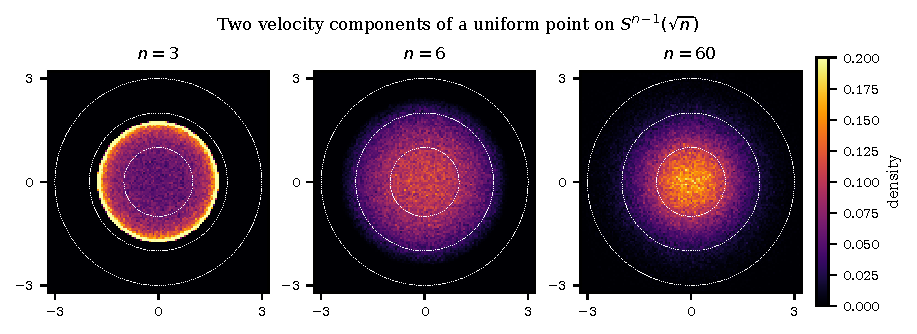
\includegraphics[width=\textwidth]{sphere_maxwell}
\caption{Joint density histogram of two coordinates of a uniform point on the sphere of radius $\sqrt{n}$ in $\R^n$, for $n=3$, $6$ and $60$ (left to right), from $200000$ points in each panel, on the square $[-3.2,3.2]^2$ and on one color scale (the bar at the right). The dotted circles of radius $1$, $2$ and $3$ are contours of the limiting standard Gaussian density. This is the energy shell of Theorem~\ref{thm:maxwellian} without the conditioning on the mean velocity. As $n$ grows the microcanonical law converges to the Maxwellian.}
\label{fig:spheremaxwell}
\end{figure}

The theorem has three readings. In kinetic theory it is the equivalence of ensembles~\cite{lanford1973,georgii1995}. In statistics it is the Bayesian statement that, after conditioning on sufficient statistics, the remaining randomness is uniform on the fiber, and its short marginals are approximately the fitted exponential family; this is the basis of conditional inference and of exact tests in exponential families. In the moment closure methods of Chapter~\ref{ch:kinetic}, it motivates Levermore's maximum entropy closure~\cite{levermore1996}: if a kinetic density is known only through finitely many moments, the conditional limit theorem selects the exponential family member with those moments as the most probable completion, which is Jaynes's maximum entropy choice~\cite{jaynes1957}. This is a heuristic and not a consequence, because the closure is a deterministic closure of a hierarchy of moment equations, whereas the theorem concerns independent particles conditioned on their moments.

\section{Bayes mixtures as universal codes}

The method of types also gives a short proof that a Bayes mixture is a good code for a family of sources. A code that assigns probability $M(x^n)$ to the binary sequence $x^n$ has length $-\log M(x^n)$, and its regret on $x^n$ is the excess of this length over the length achieved by the best Bernoulli model chosen with hindsight. We write $P_p^n(x^n) = p^k(1-p)^{n-k}$ for the probability of a sequence with $k$ ones under the Bernoulli law with parameter $p$.

\begin{theorem}[Laplace mixture]
\label{thm:laplacemixture}
Let $M(x^n) = \int_0^1p^k(1-p)^{n-k}\dd p$ be the marginal probability of a binary sequence with $k$ ones under the uniform prior. Then
\[
M(x^n) = \frac{1}{(n+1)\binom nk},\qquad-\log M(x^n)\leq n\,H\Big(\frac kn\Big)+\log(n+1).
\]
\end{theorem}

\begin{proof}
The Beta integral gives $\frac{k!(n-k)!}{(n+1)!}$, which is the first identity. By Theorem~\ref{thm:typecount}(3) with two letters, $\binom nk = |T(k/n)|\leq e^{nH(k/n)}$, which gives the bound.
\end{proof}

Since $nH(k/n) = -\log\max_p\,p^k(1-p)^{n-k}$, the Laplace mixture has regret at most $\log(n+1)$ uniformly over all sequences, and exactly $\log(n+1)$ on the two constant sequences. Its predictive law is Laplace's rule of succession~\cite{laplace1814}, derived in Section~\ref{sec:binary_definetti}, and the regret bound is also a bound on prediction. By the chain rule for relative entropy, $\E_p\log\frac{P_p^n(X^n)}{M(X^n)}$ is the sum over $i<n$ of the expected relative entropy between the Bernoulli law with parameter $p$ and the predictive law given $X^i$, and it is at most $\log(n+1)$ for every $p$, because $P_p^n(x^n)$ is at most the maximum over $p$. The average prediction error therefore tends to zero at rate $\log(n+1)/n$, uniformly in $p$, which is the information theoretic form of Bayesian consistency for this family.

Jeffreys' prior~\cite{jeffreys1946} for this family is Beta$(\frac12,\frac12)$, and its mixture is the Krichevsky Trofimov code~\cite{krichevsky1981}, which assigns probability $\Gamma(k+\frac12)\Gamma(n-k+\frac12)/(\pi\,\Gamma(n+1))$ to a sequence with $k$ ones. It does better than the uniform prior, with worst case regret $\frac12\log n+\frac12\log\pi+o(1)$, attained at the constant sequences (Exercise~\ref{ex:kt}). The smallest possible worst case regret is the minimax regret, and Shtarkov~\cite{shtarkov1987} identified the code that attains it. The normalized maximum likelihood code $\hat M(x^n) = \max_pP_p^n(x^n)/S_n$, with $S_n = \sum_{x^n}\max_pP_p^n(x^n) = \sum_{k=0}^n\binom nk(k/n)^k(1-k/n)^{n-k}$, has regret $\log S_n$ on every sequence, and every code has regret at least $\log S_n$ on some sequence, because a code with smaller regret on all sequences would give total probability more than one. By Stirling's formula $S_n = \sqrt{\pi n/2}\,(1+o(1))$, so that the minimax regret is $\frac12\log\frac{\pi n}{2}+o(1)$ (Exercise~\ref{ex:kt}), and the Krichevsky Trofimov mixture exceeds it by $\frac12\log2$, half a bit (Figure~\ref{fig:regret}).

The half bit comes from the boundary of the parameter space. For $k/n$ bounded away from $0$ and $1$ the Jeffreys mixture has regret $\frac12\log\frac{\pi n}{2}+o(1)$, the minimax value, and mixtures that add a small weight near the boundary attain the minimax regret asymptotically on every sequence, as Xie and Barron~\cite{xiebarron2000} showed. Jeffreys' prior, the reference prior of Bernardo~\cite{bernardo1979}, is optimal in another sense. The average over the prior of the expected redundancy $\E_p\log\frac{P_p^n(X^n)}{M(X^n)}$ is the mutual information between the parameter and the sample, and Clarke and Barron~\cite{clarkebarron1990,clarkebarron1994} showed that, over a compact set in the interior of the parameter space, Jeffreys' prior asymptotically maximizes it, that is, it is asymptotically least favorable, and that its mixture is asymptotically minimax for the expected redundancy.

For a smooth family of dimension $d$ the leading term of the regret is $\frac d2\log n$. Rissanen~\cite{rissanen1984} showed that, for every code and every $\varepsilon>0$, the set of parameter values at which the expected redundancy falls below $(1-\varepsilon)\frac d2\log n$ has Lebesgue measure tending to zero as $n$ grows, and for regular families $\frac d2\log n$ is also the leading term of the minimax regret~\cite{rissanen1996,xiebarron2000}. This is the minimum description length counterpart of the Bayesian information criterion~\cite{rissanen1978,schwarz1978}.

\begin{figure}[t]
\centering
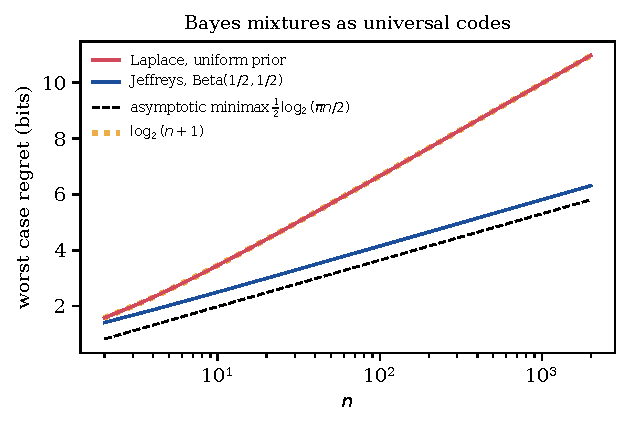
\includegraphics[width=0.85\textwidth]{regret}
\caption{Worst case regret, in bits, of the Laplace and Jeffreys mixtures for Bernoulli sequences. The Laplace curve coincides with the dotted curve $\log_2(n+1)$, which it attains at the constant sequences. The dashed curve is the asymptotic form $\frac12\log_2(\pi n/2)$ of the minimax regret of Shtarkov's code; the exact minimax regret is larger for small $n$ (for example $1.32$ bits against $0.83$ at $n=2$), and the Jeffreys curve lies half a bit above the dashed curve for large $n$.}
\label{fig:regret}
\end{figure}

\section{Hypothesis testing: Stein's lemma}

\begin{theorem}[Stein]
\label{thm:stein}
Let $X_1,\dots,X_n$ be independent with law $P_0$ under $H_0$ and $P_1$ under $H_1$, on a finite alphabet, with $P_0\ll P_1$. For $\varepsilon\in(0,1)$, let $\beta_n(\varepsilon)$ be the smallest type II error among tests with type I error at most $\varepsilon$. Then
\[
\lim_{n\to\infty}\frac1n\log\beta_n(\varepsilon) = -\KL(P_0\,\|\,P_1).
\]
\end{theorem}

\begin{proof}[Proof by types]
For the achievability, accept $H_0$ when $\KL(L_n\|P_0)\leq\delta$. Under $H_0$ this fails with probability at most $(n+1)^me^{-n\delta}$ by Theorem~\ref{thm:typecount}, so the type I error is at most $\varepsilon$ for large $n$. Under $H_1$ the acceptance probability is at most $(n+1)^m\exp(-n\min\{\KL(Q\|P_1):\KL(Q\|P_0)\leq\delta\})$, and the minimum tends to $\KL(P_0\|P_1)$ as $\delta\to0$: the minimizers converge to $P_0$ by Pinsker's inequality, and $\KL(\cdot\|P_1)$ is lower semicontinuous. For the converse, let $A_n$ be an acceptance region with $P_0^n(A_n)\geq1-\varepsilon$ and let $B_n$ be the set of $x\in A_n$ with $P_0^n(x)>0$ and $\KL(Q_x\|P_0)\leq\delta$. By the achievability computation $P_0^n(B_n)\geq(1-\varepsilon)/2$ for large $n$. For $x\in B_n$, Theorem~\ref{thm:typecount}(2) applied to $P_0$ and to $P_1$ gives
\[
\begin{aligned}P_1^n(x) &= P_0^n(x)\exp\Big(-n\sum_{a:P_0(a)>0}Q_x(a)\log\frac{P_0(a)}{P_1(a)}\Big)\\ &\geq P_0^n(x)e^{-n(\KL(P_0\|P_1)+\delta')},\end{aligned}
\]
where $\delta' = \sqrt{2\delta}\,\max_{P_0(a)>0}\big|\log\frac{P_0(a)}{P_1(a)}\big|$, because $Q_x\ll P_0\ll P_1$ and, by Pinsker's inequality, $\sum_a|Q_x(a)-P_0(a)|\leq\sqrt{2\delta}$. Hence $\beta_n\geq P_1^n(B_n)\geq\frac{1-\varepsilon}2e^{-n(\KL(P_0\|P_1)+\delta')}$, and letting $\delta\to0$ gives the lower bound on the exponent.
\end{proof}

If $P_0\not\ll P_1$, some letter $a$ has $P_0(a)>0 = P_1(a)$, and the test that accepts $H_0$ when $a$ occurs has type I error $(1-P_0(a))^n\to0$ and type II error zero, so that both sides of the theorem are $-\infty$. The theorem is the Chernoff Stein lemma~\cite{chernoff1956}; see Cover and Thomas~\cite[Section~11.8]{covertomas}.

Relative entropy is therefore the exponent of optimal discrimination, and the expected log likelihood ratio per observation, the quantity that drives the Bayes factor, is exactly this exponent. When one minimizes instead the average of the two error probabilities, the optimal exponent is the Chernoff information~\cite{chernoff1952} $C(P_0,P_1) = -\min_{0\leq s\leq1}\log\sum_xP_0(x)^sP_1(x)^{1-s}$, and the minimizing tilted law $P_s\propto P_0^sP_1^{1-s}$ is again an I projection, of $P_0$ onto the linear family $\{Q:\E_Q\log(P_1/P_0) = 0\}$ of laws equidistant in relative entropy from $P_0$ and $P_1$. Indeed, the derivative in $s$ of $\log\sum_xP_0^sP_1^{1-s}$ vanishes exactly when $\E_{P_s}\log(P_1/P_0) = 0$, and $P_s$ is a tilt of $P_0$, so that Theorem~\ref{thm:pythagoras} applies; moreover $C = \KL(P_s\|P_0) = \KL(P_s\|P_1)$ at the minimizing $s$ (Cover and Thomas~\cite[Section~11.9]{covertomas}).

\section{Types for Markov chains}

For a Markov chain on $\mathcal{X}$ with transition matrix $K$, the right notion of type is the pair type, the empirical distribution $Q^{(2)}$ of consecutive pairs $(x_i,x_{i+1})$, with first marginal $Q^{(1)}$. The two marginals of a pair type differ only through the first and last symbols of the sequence, so they agree up to $1/n$, and only pair types whose two marginals agree matter in the limit. Counting sequences with a given pair type uses an exact formula of Whittle~\cite{whittle1955} for the size of a pair type class, and the result, developed by Davisson, Longo and Sgarro~\cite{davisson1981} and by Csisz\'ar, Cover and Choi~\cite{csiszar1987}, is that the probability of a pair type with equal marginals decays, up to polynomial factors, at the rate
\[
I(Q^{(2)}) = \sum_{a,b}Q^{(2)}(a,b)\log\frac{Q^{(2)}(a,b)}{Q^{(1)}(a)K(a,b)},
\]
the relative entropy of the empirical transition law from the true one, averaged over the empirical marginal (see Csisz\'ar~\cite[Section~VII]{csiszar1998}). Contracting to the empirical marginal $\mu = Q^{(1)}$, that is, minimizing $I$ over the pair types whose two marginals equal $\mu$, gives the Donsker Varadhan rate function $-\inf_{u>0}\sum_a\mu(a)\log\frac{(Ku)(a)}{u(a)}$ of the occupation measure of the chain~\cite{donsker1975,dembozeitouni}. For a reversible process in continuous time, such as the Brownian motion of Chapter~\ref{ch:quantum}, the rate function is the Dirichlet form of $\sqrt{\dd\mu/\dd\pi}$, where $\pi$ is the invariant law, which connects large deviations with spectral gaps and, through Chapter~\ref{ch:ergodic}, with the efficiency of Monte Carlo. In discrete time the rate function is bounded below by the Dirichlet form $\frac12\sum_{a,b}\pi(a)K(a,b)\big(g(a)-g(b)\big)^2$ of $g = \sqrt{\mu/\pi}$, because $\log y\leq y-1$, but it is not equal to it: for the two state chain that flips with probability $0.3$ and $\mu = (0.2,0.8)$ the rate is $0.0851$ and the Dirichlet form is $0.0600$.

\section{Boltzmann's count revisited}

A gas of $n$ molecules whose one particle phase space is divided into $m$ cells has a type, the occupation vector divided by $n$. Under the uniform reference measure on cells, the number of microstates with type $Q$ is $|T(Q)|\approx e^{nH(Q)}$, Boltzmann's $W$. Conditioning on the total energy, a linear constraint on the type, selects with overwhelming probability the types near the I projection of the uniform law onto the energy shell, which is the Gibbs distribution, and by the conditional limit theorem the law of a single molecule converges to it, provided that the shell contains types, as when the cell energies are integers. Boltzmann's $H$ theorem~\cite{boltzmann1872}, read in this light, says that the collision dynamics carries the type of the gas toward the most numerous type compatible with the conserved quantities. This reading is ours and is not a theorem. Lanford's theorem~\cite{lanford1975} (Theorem~\ref{thm:lanford} of Chapter~\ref{ch:kinetic}) justifies the Boltzmann equation for hard spheres on a short time window, to which the $H$ theorem then applies, but it does not show that the type of the gas reaches the most numerous type, which would require the Boltzmann equation to hold over times long compared with the window, the subject of recent work of Deng, Hani and Ma~\cite{denghanima2024}. The method of types explains why the destination, if it is reached, is an exponential family.

\section*{Notes}

Csisz\'ar and K\"orner's \emph{Information Theory: Coding Theorems for Discrete Memoryless Systems}~\cite{csiszarkorner2011} develops the method of types systematically, and Csisz\'ar's survey \emph{The method of types}~\cite{csiszar1998} is a short introduction. Hoeffding~\cite{hoeffding1965} studies asymptotically optimal tests for multinomial distributions, the setting of Stein's lemma. Diaconis and Freedman~\cite{diaconisfreedman1988} give finite versions of conditional limit theorems for exponential families.

\section*{Exercises}
\begin{enumerate}
\item Prove that $|T(Q)| = n!/\prod_a(nQ(a))!$. Use Stirling's formula to show that $|T(Q)| = (2\pi n)^{-(m-1)/2}\prod_aQ(a)^{-1/2}e^{nH(Q)}(1+o(1))$ when $nQ(a)\to\infty$ for every $a$, and compare this with the bounds of Theorem~\ref{thm:typecount}(3), which hold for every type.
\item Compute the I projection of the uniform law on $\{1,\dots,6\}$ onto $\{Q:\E_Qx = 4.5\}$, Jaynes's Brandeis dice problem~\cite{jaynes1963}, and verify the Pythagorean identity numerically. The projection is $P^*(x)\propto e^{\lambda x}$ with $\lambda\approx0.371$.
\item\label{ex:ipf} Let $P$ be a law with full support on $\{1,\dots,m\}\times\{1,\dots,m'\}$ and let $r$ and $c$ be laws with full support on the two factors. Let $\pi_0 = P$, let $\pi_{t+1}$ be $\pi_t$ with its rows rescaled to have sums $r$ when $t$ is even, and with its columns rescaled to have sums $c$ when $t$ is odd (iterative proportional fitting), and let $\pi^*$ be the I projection of $P$ onto the laws with marginals $r$ and $c$. Show that rescaling the rows is the I projection onto the laws with first marginal $r$, and likewise for the columns. Show that $\KL(\pi^*\|\pi_t)$ decreases at each step, using the Pythagorean identity. Show by an example that $\KL(\pi_t\|\pi^*)$ need not decrease: for $P = \frac19\begin{pmatrix}3&2\\1&3\end{pmatrix}$, $r = (\frac12,\frac12)$ and $c = (\frac78,\frac18)$, it rises from $0.621$ to $0.625$ at the first step, while $\KL(\pi^*\|\pi_t)$ falls from $0.506$ to $0.499$.
\item Verify the exact conditional density of the exponential example and the value of the constant $c$ in its total variation rate.
\item\label{ex:kt} Show that the Krichevsky Trofimov mixture assigns probability $\frac{\Gamma(k+\frac12)\Gamma(n-k+\frac12)}{\pi\,\Gamma(n+1)}$ to a sequence with $k$ ones, and derive its worst case regret. Show that the regret is largest on the constant sequences, where it is $\frac12\log(\pi n)+o(1)$ (treat $k$ as a continuous variable and use $\psi'(x+\frac12)<1/x$ for the digamma function $\psi$), and that Shtarkov's sum satisfies $S_n = \sqrt{\pi n/2}\,(1+o(1))$ by Stirling's formula.
\item Compute the Chernoff information between $\mathrm{Bernoulli}(p)$ and $\mathrm{Bernoulli}(q)$ and the optimal tilting parameter.
\end{enumerate}


\part{Brownian Motion, Mixtures and Entropy}\label{part:brownian}
\chapter{Brownian Motion and Yor's Identities as Algorithms}
\label{ch:brownian}

\section{From pollen to paths}

Robert Brown observed in 1827~\cite{brown1828} the irregular motion of particles ejected from pollen grains and showed that it persisted in inorganic dust, ruling out a vital origin. For seventy years the phenomenon had no theory. Bachelier in 1900~\cite{bachelier1900} gave the mathematics without the physics. Einstein in 1905~\cite{einstein1905} and Smoluchowski in 1906~\cite{smoluchowski1906} gave the physics: the motion is caused by the thermal agitation of the molecules of the fluid, the mean squared displacement grows linearly in time, and the constant of proportionality is related to temperature and viscosity by
\begin{equation}
D = \frac{k_B T}{6\pi\eta a},
\label{eq:einstein_relation}
\end{equation}
for a sphere of radius $a$ in a fluid of viscosity $\eta$. Since $k_B = R/N_A$, a measurement of $D$ is a measurement of Avogadro's number. Perrin's experiments of 1908 and 1909~\cite{perrin1908,perrin1909} did exactly this and convinced the remaining skeptics, Ostwald among them, of the reality of atoms. Langevin in 1908~\cite{langevin1908} rederived Einstein's result from Newton's law with a random force, introducing the first stochastic differential equation. Wiener in 1923~\cite{wiener1923} constructed the process as a probability measure on continuous paths. Kolmogorov in 1931~\cite{kolmogorov1931} wrote down the forward and backward equations for general diffusions. L\'evy, Feller, It\^o and Doob completed the theory.

Einstein's argument is the sixth problem in miniature. A macroscopic law, diffusion with coefficient $D$, is derived from microscopic collisions; the derivation passes through a probability distribution on the motion of a single particle; and the macroscopic constant encodes a microscopic quantity, the size of molecules, that can be inferred from macroscopic observations.

\section{Construction}

\begin{definition}
A standard Brownian motion is a process $(B_t)_{t\geq0}$ with $B_0 = 0$, continuous paths, and independent Gaussian increments $B_t - B_s\sim N(0,t-s)$.
\end{definition}

The most algorithmic construction is due to L\'evy and Ciesielski. Let $h_{0}=\mathbb{1}_{[0,1]}$ and, for $n\geq0$ and $0\leq k<2^n$, let $h_{n,k} = 2^{n/2}\big(\mathbb{1}_{[k2^{-n},(k+\frac12)2^{-n})} - \mathbb{1}_{[(k+\frac12)2^{-n},(k+1)2^{-n})}\big)$ be the Haar functions, an orthonormal basis of $L^2[0,1]$. Their integrals $S_{n,k}(t) = \int_0^t h_{n,k}$ are the Schauder tent functions, of height $2^{-n/2-1}$ and support of length $2^{-n}$.

\begin{theorem}[L\'evy, Ciesielski]
\label{thm:levy_ciesielski}
Let $N_0$ and $N_{n,k}$ be independent standard normal variables. The series
\[
B_t = N_0\,t + \sum_{n=0}^\infty\sum_{k=0}^{2^n-1} N_{n,k}\,S_{n,k}(t)
\]
converges uniformly on $[0,1]$ almost surely, and its sum is a standard Brownian motion on $[0,1]$.
\end{theorem}

\begin{proof}
For fixed $n$ the tents $S_{n,k}$ have disjoint supports, so $\sup_t\big|\sum_k N_{n,k}S_{n,k}(t)\big|\leq 2^{-n/2-1}\max_k|N_{n,k}|$. Since $\P(\max_k|N_{n,k}|>2\sqrt{n})\leq 2^n e^{-2n}$, which is summable, Borel Cantelli shows that the $n$th level is eventually bounded by $\sqrt{n}2^{-n/2}$, a summable sequence. The limit is therefore continuous. It is a centered Gaussian process with covariance
\[
\E B_sB_t = \sum_{\phi}\int_0^s\phi\int_0^t\phi = \langle\mathbb{1}_{[0,s]},\mathbb{1}_{[0,t]}\rangle_{L^2} = s\wedge t,
\]
by Parseval's identity for the Haar basis.
\end{proof}

Truncating the series of Theorem~\ref{thm:levy_ciesielski} after level $n$ gives an exact sample of Brownian motion at the dyadic points $k2^{-(n+1)}$, linearly interpolated in between.

\section{The heat equation and the generator}

The transition density $p_t(x,y) = (2\pi t)^{-1/2}e^{-(y-x)^2/2t}$ solves $\partial_t p = \frac12\partial_y^2 p$. For a diffusion $\dd X_t = b(X_t)\dd t + \sigma(X_t)\dd B_t$, It\^o's formula shows that $u(t,x) = \E_x f(X_t)$ solves the backward equation $\partial_t u = \mathcal{L}u$ with $\mathcal{L} = b\,\partial_x + \frac12\sigma^2\partial_x^2$, and the law $\rho_t$ of $X_t$ solves the forward, or Fokker Planck, equation $\partial_t\rho = \mathcal{L}^*\rho$. The Ornstein Uhlenbeck process $\dd X_t = -X_t\dd t+\sqrt2\dd B_t$ has the standard Gaussian as invariant law and the semigroup used in the proof of Theorem~\ref{thm:gaussian_poincare}.

\section{Langevin, Ornstein Uhlenbeck and the high friction limit}

Langevin's equation for a particle of mass $m$ subject to friction $\zeta$ and thermal noise reads
\[
\dd X_t = V_t\dd t,\qquad m\,\dd V_t = -\zeta V_t\dd t + \sqrt{2\zeta k_BT}\,\dd B_t.
\]
The velocity is an Ornstein Uhlenbeck process with stationary law $N(0,k_BT/m)$, the one dimensional Maxwellian. The position is not Markov. Integrating,
\[
X_t - X_0 = \frac{\sqrt{2\zeta k_B T}}{\zeta}B_t + \frac{m}{\zeta}(V_0 - V_t),
\]
so in the limit $m/\zeta\to0$ (high friction, the Smoluchowski Kramers limit) the position converges to a Brownian motion with diffusion coefficient $D = k_BT/\zeta$, which is Einstein's relation \eqref{eq:einstein_relation} once Stokes's law $\zeta = 6\pi\eta a$ is used. This is a rigorous passage from a mechanical model with friction to diffusion. The deeper question, whether Langevin's friction and noise can themselves be derived from deterministic collisions, is a genuine instance of the sixth problem. Bodineau, Gallagher and Saint Raymond~\cite{bgs2016} proved a version of it for $N$ identical hard spheres of diameter $\varepsilon$ in dimension $d$: in the limit $N\to\infty$, $\varepsilon\to0$ with $N\varepsilon^{d-1}\to\infty$ and a suitable diffusive scaling of the observation time, a tagged particle converges to Brownian motion. All particles have the same mass, so this derives a Brownian limit from deterministic collisions but does not derive Langevin's friction for a heavy particle in a bath of light ones.

\section{Bessel processes and time change}

For $\delta\geq0$ the squared Bessel process of dimension $\delta$ is the solution of
\[
\dd Z_t = \delta\dd t + 2\sqrt{Z_t}\dd B_t,\qquad Z_t\geq0.
\]
For integer $\delta$ it is the squared norm of a $\delta$ dimensional Brownian motion. Two structural facts make it central.

\begin{theorem}[Additivity, Shiga and Watanabe]
If $Z$ and $Z'$ are independent squared Bessel processes of dimensions $\delta,\delta'$ started at $z,z'$, then $Z+Z'$ is a squared Bessel process of dimension $\delta+\delta'$ started at $z+z'$.
\end{theorem}

\begin{proof}
$\dd(Z+Z') = (\delta+\delta')\dd t + 2\sqrt{Z}\dd B + 2\sqrt{Z'}\dd B'$, and the martingale part has quadratic variation $4(Z+Z')\dd t$, so it equals $2\sqrt{Z+Z'}\dd W$ for a Brownian motion $W$ by L\'evy's characterization. Pathwise uniqueness for the squared Bessel equation, which holds by the Yamada Watanabe criterion, identifies the law.
\end{proof}

Additivity means the laws form a convolution semigroup in both $\delta$ and the starting point: squared Bessel laws are infinitely divisible, and their Laplace transforms are
\[
\E_z e^{-\lambda Z_t} = (1+2\lambda t)^{-\delta/2}\exp\Big(-\frac{\lambda z}{1+2\lambda t}\Big).
\]
At $z=0$ this is the Laplace transform of a Gamma law with shape $\delta/2$ and scale $2t$, the first appearance of the Gamma family that pervades the companion volume on Hilbert's eighth problem.

The square root of a squared Bessel process of dimension $\delta$ is a Bessel process of dimension $\delta$, and it is convenient to index it by $\nu = \delta/2-1$. For every real $\nu$, the Bessel process of index $\nu$ started at $r>0$ is the solution of
\[
\dd R_u = \dd\beta_u + \Big(\nu+\frac12\Big)\frac{\dd u}{R_u},\qquad R_0 = r,
\]
with $\beta$ a Brownian motion, run until it first hits zero. By Itô's formula $R^2$ solves the squared Bessel equation of dimension $2\nu+2$. For $\nu\geq0$ the process never reaches zero, and for $\nu<0$ it reaches zero in finite time.

\begin{theorem}[Lamperti~\cite{lamperti1972}]
\label{thm:lamperti}
For $\nu\in\R$ let $A_t = \int_0^t e^{2(B_s+\nu s)}\dd s$. There is a Bessel process $R$ of index $\nu$ (dimension $2\nu+2$) started at $1$ such that
\[
e^{B_t + \nu t} = R_{A_t},\qquad t\geq0.
\]
If $\nu<0$, then $A_\infty = \lim_{t\to\infty}A_t$ is finite and is the time at which $R$ hits zero.
\end{theorem}

\begin{proof}
Put $X_t = B_t+\nu t$. The map $t\mapsto A_t$ is a $C^1$ bijection of $[0,\infty)$ onto $[0,A_\infty)$ with derivative $e^{2X_t}>0$. Let $C$ be its inverse and set $R_u = e^{X_{C_u}}$ for $u<A_\infty$, so that $R_{A_t} = e^{X_t}$. Itô's formula gives $e^{X_t} = 1+M_t+(\nu+\frac12)\int_0^te^{X_s}\dd s$, where $M_t = \int_0^te^{X_s}\dd B_s$ is a continuous local martingale with $\langle M\rangle_t = A_t$. By the Dambis, Dubins and Schwarz theorem, $\beta_u = M_{C_u}$ is a Brownian motion (on an enlarged probability space if $A_\infty<\infty$). The substitution $s = C_v$, $\dd s = e^{-2X_{C_v}}\dd v$, gives $\int_0^{C_u}e^{X_s}\dd s = \int_0^uR_v^{-1}\dd v$, so $R_u = 1+\beta_u+(\nu+\frac12)\int_0^uR_v^{-1}\dd v$, which is the equation of a Bessel process of index $\nu$ started at $1$. If $\nu<0$, then $X_t\to-\infty$ linearly in $t$, so $e^{2X_t}$ is integrable and $A_\infty<\infty$, while $R_u = e^{X_{C_u}}\to0$ as $u\uparrow A_\infty$ because $C_u\to\infty$.
\end{proof}

Lamperti's relation converts questions about geometric Brownian motion, the model of Black and Scholes and the descendant of Bachelier's model, into questions about Bessel processes, and conversely. Combined with time reversal and the theory of last exit times, it generates a large family of identities in law.

\begin{theorem}[Dufresne~\cite{dufresne1990}]
\label{thm:dufresne}
For $\mu>0$,
\[
\int_0^\infty e^{2(B_s - \mu s)}\dd s \eqd \frac{1}{2\gamma_\mu},
\]
where $\gamma_\mu$ has the Gamma law with shape $\mu$ and unit scale.
\end{theorem}

The identity and its relatives are surveyed in~\cite{matsumotoyor2005}.

\begin{proof}
By Theorem~\ref{thm:lamperti} with $\nu=-\mu$, the integral is the time $T_0$ at which a Bessel process of index $-\mu$ started at $1$ hits zero. For $\lambda>0$ let $u(x) = \E_xe^{-\lambda T_0}$ be the Laplace transform of this hitting time when the process starts at $x>0$. By scaling, $T_0$ under $\P_x$ has the law of $x^2T_0$ under $\P_1$, so $0\leq u\leq1$ and $u(0+)=1$. Since $e^{-\lambda t}u(R_t)$ is a martingale up to $T_0$, $u$ solves $\frac12u''+\frac{1-2\mu}{2x}u' = \lambda u$. The substitution $u(x) = x^\mu w(x)$ turns this into $x^2w''+xw'-(2\lambda x^2+\mu^2)w=0$, the modified Bessel equation of order $\mu$ in the variable $cx$ with $c = \sqrt{2\lambda}$, and the solutions with $u$ bounded are the multiples of $x^\mu K_\mu(cx)$. Since $K_\mu(z)\sim\frac12\Gamma(\mu)(z/2)^{-\mu}$ as $z\downarrow0$, the condition $u(0+)=1$ gives $u(x) = (cx)^\mu K_\mu(cx)/(2^{\mu-1}\Gamma(\mu))$. On the other hand, $K_\mu(z) = \frac12(z/2)^{-\mu}\int_0^\infty e^{-g-z^2/4g}g^{\mu-1}\dd g$~\cite[10.32.10]{dlmf}, and with $z=c$ this gives $\E e^{-\lambda/(2\gamma_\mu)} = \Gamma(\mu)^{-1}\int_0^\infty e^{-g-\lambda/2g}g^{\mu-1}\dd g = u(1)$. Laplace transforms determine laws.
\end{proof}

\section{Yor's identities as algorithms}

Marc Yor and his school produced hundreds of identities of the form $X\eqd F(Y_1,\dots,Y_m)$ where $X$ is a functional of Brownian motion and the $Y_i$ are elementary independent variables, Gamma, Beta, normal or exponential. In our paper \emph{Yor's Identities as Algorithms}~\cite{polsonsokolovyor} we read each such identity as an exact simulation algorithm: to sample $X$, sample the $Y_i$ and apply $F$. No discretization, no Markov chain and no rejection step is required. The identity is a proof of correctness for the algorithm, and the algorithm is a numerical certificate for the identity.

Theorem~\ref{thm:dufresne} is an example: the perpetuity $\int_0^\infty e^{2(B_s-\mu s)}\dd s$, which arises in the pricing of perpetual Asian options and in the theory of diffusions in random environments, is sampled exactly by one Gamma draw. A second example is Pitman's theorem~\cite{pitman1975}, $2M_t - B_t\eqd R_t$ as processes, where $M$ is the running maximum and $R$ a three dimensional Bessel process; it converts a path functional into a Markov process that can be sampled by summing three independent Brownian motions in quadrature.

\subsubsection{Identities as samplers} An identity in law $X\eqd F(Y_1,\dots,Y_m)$ is an algorithm for sampling $X$ when three conditions hold. The variables $Y_i$ can be drawn exactly at the cost of a few random numbers, the map $F$ is explicit, and the identity holds for the whole functional $X$ and not only asymptotically in a parameter. Table~\ref{tab:yor_catalogue} lists eight identities; the last three fall short of the conditions, as explained after the table.

\begin{table}[t]\centering\footnotesize\setlength{\tabcolsep}{3pt}
\caption{Identities in law read as samplers.}\label{tab:yor_catalogue}
\begin{tabular}{@{}>{\raggedright\arraybackslash}p{0.95in}>{\raggedright\arraybackslash}p{1.85in}>{\raggedright\arraybackslash}p{1.15in}>{\raggedright\arraybackslash}p{0.34in}@{}}
\toprule
Identity & Statement in law & Sampler & Cost\\
\midrule
Dufresne, 1990~\cite{dufresne1990}, Theorem~\ref{thm:dufresne} & $\int_0^\infty e^{2(B_s-\mu s)}\dd s\eqd 1/(2\gamma_\mu)$ for $\mu>0$ & Draw $\gamma_\mu$; return $1/(2\gamma_\mu)$ & 1\\
Bougerol, 1983~\cite{bougerol1983,alili1997} & $\sinh B_t\eqd\beta_{A_t}$ for fixed $t$, with $\beta$ a Brownian motion independent of $B$ & Draw $Z$; return $\sinh(\sqrt tZ)$, a draw of $\beta_{A_t}$, not of $A_t$ & 1\\
Bachelier, 1900, and Pitman, 1975~\cite{bachelier1900,pitman1975} & $\P(M_t\ge m\mid B_t=b)=e^{-2m(m-b)/t}$ for $m\ge\max(b,0)$; $2M-B$ is $\mathrm{BES}(3)$ & Draw $Z$, $U$; return $B_t$ and $M_t$ (Algorithm~\ref{alg:yor_maximum}) & 2\\
Michael, Schucany and Haas, 1976~\cite{michael1976} & $\inf\{t:B_t+\nu t=a\}$ for $a,\nu>0$ is inverse Gaussian with mean $a/\nu$ and shape $a^2$ & Draw $Z$, $U$; return a root of a quadratic in $Z^2$ (Algorithm~\ref{alg:yor_passage}) & 2\\
Polson and Sokolov, 2026~\cite{polsonsokolovyor,carvalho2010} & Horseshoe: $\lambda^2\eqd\gamma_{1/2}/\gamma'_{1/2}$ is a GGC with Thorin mass $\frac12$, and $\E e^{-s\lambda^2}=e^s\,\mathrm{erfc}\sqrt s$ & Draw $\gamma_{1/2}$, $\gamma'_{1/2}$; return the ratio & 2\\
Ciesielski and Taylor, 1962, and Kent, 1980~\cite{ciesielski1962,kent1980} & Theorem~\ref{thm:exit_series}: $T\eqd\int_0^\infty\mathbb{1}_{\{|W_s|<1\}}\dd s\eqd\sum_{n\ge1}8E_n/((2n-1)^2\pi^2)$ & Draw $E_1,\dots,E_K$ and a Gamma tail; return the sum & $K+1$\\
Dufresne, 2001, and Matsumoto and Yor, 2001, in~\cite{matsumotoyor2005} & $1/A^{(-\mu)}_t\eqd 1/A^{(\mu)}_t+2\gamma_\mu$ for $\mu>0$ and each $t$, with $\gamma_\mu$ independent of $B$ & Draw $\gamma_\mu$; add $2\gamma_\mu$ to $1/A^{(\mu)}_t$ and invert & 1, and $A^{(\mu)}_t$\\
Biane, Pitman and Yor, 2001~\cite{bpy2001} & Theorem~\ref{thm:bpy}: $\E Y^s=2\xi(s)$ for $s\in\C$, where $Y=\sqrt{2/\pi}\,m$ and $m$ is an excursion maximum & n/a & n/a\\
\bottomrule
\end{tabular}
\end{table}

\subsubsection{Reading the table} In the table $M_t=\max_{s\le t}B_s$, $A^{(\nu)}_t=\int_0^te^{2(B_s+\nu s)}\dd s$ and $A_t=A^{(0)}_t$; $\gamma_\mu$ is a Gamma variable with shape $\mu$ and unit scale and $\gamma'_\mu$ is an independent copy; $E_n$, $Z$ and $U$ are standard exponential, standard normal and uniform variables, independent of each other and of $B$; $T$ is the exit time of $B$ from $(-1,1)$ and $W$ is three dimensional Brownian motion. The cost is counted in random variates, and $\mathrm{BES}(3)$ is the three dimensional Bessel process. In the horseshoe row the mixing law is HCM and hence a GGC by Chapter~\ref{ch:mixtures}; the sampler does not use that structure. In the exit time row the Gamma variable matches only the mean and variance of the tail after $K$ terms, so the sum is not exact. The Matsumoto and Yor row is Theorem~5.1 of Part~II of~\cite{matsumotoyor2005}, which credits the identity at a fixed $t$ to Dufresne and the extension to processes in $t$ to Matsumoto and Yor, both in 2001; it moves exactness from one functional to the other, since a sampler of $A^{(-\mu)}_t$ needs one of $A^{(\mu)}_t$, and letting $t\to\infty$ gives the Dufresne row. The Biane, Pitman and Yor row concerns the moments of $Y$ and gives no sampler.

\subsubsection{Four algorithms} Algorithm~\ref{alg:yor_dufresne} replaces the $T/h$ normal variates of an Euler sum for the perpetuity by one Gamma variate and needs no horizon $T$.

\begin{samepage}
\begin{algorithm}[Perpetuity of geometric Brownian motion]\label{alg:yor_dufresne}
Input: $\mu>0$. Output: one draw of $\int_0^\infty e^{2(B_s-\mu s)}\dd s$. Random variates: one Gamma. Rests on Theorem~\ref{thm:dufresne}, the Dufresne row of Table~\ref{tab:yor_catalogue}.
\begin{enumerate}[nosep]
\item Draw $G$ from the Gamma law with shape $\mu$ and unit scale.
\item Return $X=1/(2G)$.
\end{enumerate}
\end{algorithm}
\end{samepage}

Bougerol's identity~\cite{bougerol1983} says that $\sinh B_t\eqd\beta_{A_t}$ for each fixed $t$, with $\beta$ a Brownian motion independent of $B$ and $A_t=\int_0^te^{2B_s}\dd s$ (Theorem~3.1 of Part~I of~\cite{matsumotoyor2005}). It is not an identity of processes in $t$, since $\sinh B_t$ is not a martingale and $\beta_{A_t}$ is. Given $A_t$ the variable $\beta_{A_t}$ is $N(0,A_t)$, so the right side is a normal variance mixture with mixing variable $A_t$, and Algorithm~\ref{alg:yor_bougerol} draws from it, without drawing $A_t$, as the hyperbolic sine of a normal variable, a Johnson $S_U$ variable. Alili, Dufresne and Yor~\cite{alili1997} gave a short proof by It\^o's formula and extended the identity to Brownian motion with drift;~\cite{vakeroudis2012} is a survey.

\begin{samepage}
\begin{algorithm}[Brownian motion at an exponential functional]\label{alg:yor_bougerol}
Input: $t>0$. Output: one draw of $\beta_{A_t}$, a Brownian motion read at the random time $A_t=\int_0^te^{2B_s}\dd s$; it does not return $A_t$. Random variates: one normal. Rests on Bougerol's identity, the Bougerol row of Table~\ref{tab:yor_catalogue}.
\begin{enumerate}[nosep]
\item Draw $Z$ from the standard normal law.
\item Return $S=\sinh(\sqrt tZ)$.
\end{enumerate}
\end{algorithm}
\end{samepage}

For $m>0$ and $b\le m$ the reflection principle, Theorem~\ref{thm:reflection}, gives $\P(M_t\ge m,B_t\le b)=\P(B_t\ge2m-b)$. Differentiating in $b$ and dividing by the density $\varphi_t(b)$ of $B_t$ gives $\P(M_t\ge m\mid B_t=b)=\varphi_t(2m-b)/\varphi_t(b)=e^{-2m(m-b)/t}$ for $m\ge\max(b,0)$. Setting this equal to $U$ and taking the larger root of the quadratic in $m$ gives step 3 of Algorithm~\ref{alg:yor_maximum}. Differentiating in $m$ as well gives the joint density $2r(2\pi t^3)^{-1/2}e^{-r^2/(2t)}$ of $(M_t,R_t)$ on $0\le m\le r$, where $R_t=2M_t-B_t$. It does not depend on $m$, so given $R_t$ the maximum is uniform on $[0,R_t]$, and $R_t$ has the law of $\sqrt t$ times the norm of a standard normal vector in $\R^3$, in agreement with Pitman's theorem~\cite{pitman1975} for the process $2M-B$. This is a second exact route to $(B_t,M_t)$ at the same cost: draw $R_t=\sqrt{2t\gamma_{3/2}}$, put $M_t=VR_t$ with $V$ uniform on $(0,1)$ and $B_t=2M_t-R_t$.

\begin{samepage}
\begin{algorithm}[Brownian motion and its maximum]\label{alg:yor_maximum}
Input: $t>0$. Output: one draw from the joint law of $(B_t,M_t)$. Random variates: one normal and one uniform. Rests on Theorem~\ref{thm:reflection}.
\begin{enumerate}[nosep]
\item Draw $Z$ from the standard normal law and $U$ uniform on $(0,1]$, independently.
\item Put $B_t=\sqrt tZ$.
\item Put $M_t=\frac12\big(B_t+\sqrt{B_t^2-2t\log U}\big)$ and return $(B_t,M_t)$.
\end{enumerate}
\end{algorithm}
\end{samepage}

Let $\nu>0$ and let $T_a$ be the first time at which $B_t+\nu t$ reaches $a>0$. Girsanov's theorem multiplies the density of the L\'evy law of the hitting time of $a$ by $e^{\nu a-\nu^2t/2}$, which gives the inverse Gaussian density $a(2\pi t^3)^{-1/2}\exp(-(a-\nu t)^2/(2t))$ with mean $a/\nu$ and shape $a^2$. For this law $(\nu T_a-a)^2/T_a$ has the $\chi^2$ law with one degree of freedom, so it has the law of $Y=Z^2$. Indeed, the distribution function of $T_a$ is $F(t)=\Phi((\nu t-a)/\sqrt t)+e^{2a\nu}\Phi(-(\nu t+a)/\sqrt t)$, where $\Phi$ is the standard normal distribution function, and for $y>0$ the equation $(\nu t-a)^2=yt$ has two positive roots $t_1<a/\nu<t_2$. At them $(\nu t-a)/\sqrt t$ equals $-\sqrt y$ and $\sqrt y$, and $(\nu t+a)/\sqrt t=\sqrt{y+4a\nu}$ at both, so $\P((\nu T_a-a)^2/T_a\le y)=F(t_2)-F(t_1)=\Phi(\sqrt y)-\Phi(-\sqrt y)$. Given the value $Y$ of $(\nu T_a-a)^2/T_a$, the variable $T_a$ is therefore one of the two roots of $(\nu t-a)^2=Yt$, the smaller root $X$ and the larger root $a^2/(\nu^2X)$, since the product of the roots is $a^2/\nu^2$. Michael, Schucany and Haas~\cite{michael1976} show that $T_a$ may be taken equal to the smaller root $X$ with probability $a/(a+\nu X)$ and to the larger root otherwise, which is Algorithm~\ref{alg:yor_passage}. In floating point arithmetic the smaller root is better computed as $X=2a^2/(2a\nu+Y+\sqrt{Y^2+4a\nu Y})$, the same number without the cancellation that makes the expression of step 2 inaccurate when $a\nu$ is small compared with $Y$.

\begin{samepage}
\begin{algorithm}[First passage time with drift]\label{alg:yor_passage}
Input: $a>0$ and $\nu>0$. Output: one draw of $T_a=\inf\{t:B_t+\nu t=a\}$. Random variates: one normal and one uniform. Rests on the inverse Gaussian law of $T_a$ and the transformation with multiple roots of Michael, Schucany and Haas, the passage time row of Table~\ref{tab:yor_catalogue}.
\begin{enumerate}[nosep]
\item Draw $Z$ from the standard normal law and put $Y=Z^2$.
\item Put $X=\dfrac{a}{\nu}+\dfrac{Y-\sqrt{Y^2+4a\nu Y}}{2\nu^2}$.
\item Draw $U$ uniform on $(0,1)$. If $U\le a/(a+\nu X)$ return $X$, and otherwise return $a^2/(\nu^2X)$.
\end{enumerate}
\end{algorithm}
\end{samepage}

\subsubsection{Checks} We compared each sampler with the exact distribution function and with the Euler scheme that it replaces, by the Kolmogorov Smirnov distance $\sup_x|F_n(x)-F(x)|$ between the empirical distribution function $F_n$ of $10^5$ draws and the exact one $F$. For an exact sample of this size the distance has mean 0.0027 and exceeds 0.0043 with probability 0.05. The generator is NumPy's \textit{default\_rng} with seed 20261007 and a fixed offset for each experiment, and the script \textit{code/yor\_catalogue.py} in the \LaTeX\ source reproduces the numbers below, apart from the times, in about two minutes on one core. The Euler schemes use nested grids of the same Brownian paths: left endpoint Riemann sums for $\int_0^6e^{2(B_s-2s)}\dd s$ and for $A_1$, the latter times an independent normal variable for Bougerol's identity with $t=1$, the maximum over the grid for $M_1$, and the first grid time with $B_{kh}+kh\ge1$ for $T_1$ with $\nu=1$.

\begin{table}[t]\centering\footnotesize\setlength{\tabcolsep}{4pt}
\caption{Kolmogorov Smirnov distance between $10^5$ draws and the exact distribution function, for the exact sampler and for Euler schemes with step $h$.}\label{tab:yor_checks}
\begin{tabular}{@{}lccccc@{}}
\toprule
& Exact & $h=2^{-6}$ & $h=2^{-8}$ & $h=2^{-10}$ & $h=2^{-12}$\\
\midrule
Perpetuity, $\mu=2$ & 0.0041 & 0.0243 & 0.0086 & 0.0051 & 0.0043\\
Bougerol, $t=1$ & 0.0024 & 0.0024 & 0.0025 & 0.0025 & 0.0025\\
Maximum $M_1$ & 0.0044 & 0.0701 & 0.0353 & 0.0175 & 0.0086\\
Passage time, $a=\nu=1$ & 0.0022 & 0.0575 & 0.0283 & 0.0154 & 0.0096\\
\bottomrule
\end{tabular}
\end{table}

The exact samplers in Table~\ref{tab:yor_checks} have distances between 0.0022 and 0.0044, the largest being just above the 5\% value, for the maximum, and over 40 repetitions with fresh seeds of each of six exact samplers and coordinates, 14 of the 240 distances exceed it, against 12 expected. The Riemann sums have errors of order $h$: the exact mean of the sum differs from its limit by 1.6\% at $h=2^{-6}$ and 0.024\% at $h=2^{-12}$, for the perpetuity and for $A_1$, and the distance for the perpetuity falls from 0.024 to 0.0043. The Bougerol distance is at the noise level for every $h$, so it does not detect this error. The maximum and the first passage time on a grid have errors of order $\sqrt h$, and their distances fall by factors between 1.6 and 2.0 for each fourfold reduction of $h$; the distance for the maximum is the fraction of paths whose grid maximum is zero, about $\sqrt{h/\pi}$, and an exact maximum is never zero. The Kent series cut after $K=1,2,4,8,16$ terms has distances 0.175, 0.091, 0.047, 0.025 and 0.013, and at most 0.0039 for all five values when the Gamma tail is added. The Matsumoto and Yor row, with $\mu=t=1$ and $5\times10^4$ Euler paths with $h=2^{-10}$ on each side, has a two sample distance of 0.0059 against a 5\% value of 0.0086. The moments $\E Y^s$ computed from the theta series for the distribution function of the excursion maximum agree with $2\xi(s)$ for $s=1,2,3,4$ to within $5\times10^{-16}$. For the horseshoe row, the Laplace transform of $10^6$ draws of $\gamma_{1/2}/\gamma'_{1/2}$ is within 0.0004 of $e^s\,\mathrm{erfc}\sqrt s$ at $s=0.1,1,10$, and $-\log(e^s\,\mathrm{erfc}\sqrt s)$ exceeds $\frac12\log(\pi s)$ by 0.0049, $5\times10^{-5}$ and $5\times10^{-7}$ at $s=10^2,10^4,10^6$, consistent with the Thorin mass $\frac12$. In NumPy on one core of an Apple M2, $10^5$ exact draws took 1.8 to 2.8 milliseconds of CPU time and $10^5$ Euler paths with $h=2^{-10}$ took 1.5 to 13 seconds, so the exact samplers were faster by factors between $5\times10^2$ and $6\times10^3$. Times depend on the machine and on its load, and the factors depend on them less.

\subsubsection{A library} The table is the start of the library that Open Problem~\ref{prob:yor} asks for. A solution of the problem would replace the Gamma variable of the exit time row by an exact draw of the tail. At $10^5$ draws the checks above cannot tell the Gamma tail from the exact one, which is evidence that the approximation is good and not a proof that it is exact.


\section{Exit times and infinite sums of exponentials}

Let $T = \inf\{t: |B_t| = 1\}$ be the exit time of standard Brownian motion from $(-1,1)$. Since $e^{\sqrt{2\lambda}B_t - \lambda t}$ and $e^{-\sqrt{2\lambda}B_t-\lambda t}$ are martingales, their average $\cosh(\sqrt{2\lambda}B_t)e^{-\lambda t}$ is a martingale, and optional stopping at $T$ gives
\begin{equation}
\E e^{-\lambda T} = \frac{1}{\cosh\sqrt{2\lambda}}.
\label{eq:exit_laplace}
\end{equation}
The Weierstrass product $\cosh z = \prod_{n\geq1}\big(1 + \frac{4z^2}{(2n-1)^2\pi^2}\big)$ then yields a structure theorem for $T$.

\begin{theorem}[Exit time as a series of exponentials]
\label{thm:exit_series}
Let $E_1,E_2,\dots$ be independent standard exponential variables. Then
\[
T\eqd\sum_{n=1}^\infty\frac{8}{(2n-1)^2\pi^2}E_n.
\]
Equivalently $T\eqd 4\,\omega$ where $\omega$ has the P\'olya Gamma law $PG(1,0)$ of Polson, Scott and Windle~\cite{psw2013}. The density of $T$ is
\[
f_T(t) = \frac{\pi}{2}\sum_{n=0}^\infty(-1)^n(2n+1)\exp\Big(-\frac{(2n+1)^2\pi^2}{8}t\Big),\qquad t>0.
\]
\end{theorem}

\begin{proof}
The Laplace transform of the series is $\prod_n(1+8\lambda/((2n-1)^2\pi^2))^{-1}$, which equals $1/\cosh\sqrt{2\lambda}$ by the product formula with $z^2 = 2\lambda$. The series converges almost surely since its mean $\sum 8/((2n-1)^2\pi^2) = 1$ is finite, consistent with $\E T = 1$. The P\'olya Gamma law $PG(1,0)$ is defined by $\omega = \frac{1}{2\pi^2}\sum_n E_n/(n-\frac12)^2$, and $4\omega$ has coefficients $\frac{2}{\pi^2(n-\frac12)^2} = \frac{8}{\pi^2(2n-1)^2}$. For the density, $1/\cosh\sqrt{2\lambda}$ has simple poles at $\lambda_n = -(2n+1)^2\pi^2/8$ with residues $(-1)^n(2n+1)\pi/2$, obtained by differentiating $\cosh\sqrt{2\lambda}$ at the poles; partial fractions and Laplace inversion give the series.
\end{proof}

Figure~\ref{fig:exit} compares three computations of the law of $T$. The series algorithm is exact up to truncation, and the truncation error after $K$ terms has mean $\sum_{n>K}8/((2n-1)^2\pi^2)\approx 2/(\pi^2K)$, which can be corrected by a single Gamma variable matched in mean and variance.

\begin{figure}[t]
\centering
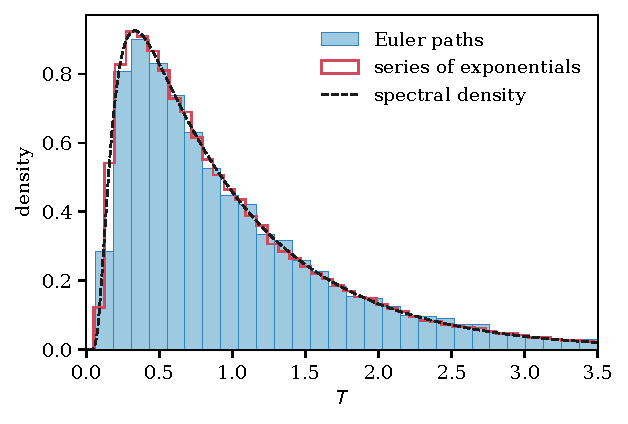
\includegraphics[width=0.92\textwidth]{exit_time}
\caption{The exit time of Brownian motion from $(-1,1)$. Histograms of 6000 paths simulated by the Euler scheme with step $2\times10^{-4}$ and of 60000 draws of the series of exponentials of Theorem~\ref{thm:exit_series} truncated at 200 terms, and the density of the theorem summed over 200 terms.}
\label{fig:exit}
\end{figure}

The theorem is a special case of a general principle due to Kent~\cite{kent1980}. For a regular one dimensional diffusion started at a reflecting or entrance boundary $a$, the hitting time of a level $b$ is distributed as $\sum_n E_n/\lambda_n$, where $0<\lambda_1<\lambda_2<\cdots$ are the eigenvalues of minus the generator on $(a,b)$ with Dirichlet condition at $b$ and the natural condition at $a$. Hitting times are therefore infinitely divisible, indeed generalized Gamma convolutions in the sense of Chapter~\ref{ch:mixtures}, and their L\'evy measures are determined by the spectrum. Krein's theory of strings, in the form given by Kotani and Watanabe~\cite{kotani1982}, runs the other way: a diffusion in natural scale with given boundary conditions is determined by its spectral measure, which records the eigenvalues together with their norming constants. The companion volume~\cite{polsonh8} uses this inverse spectral correspondence for the Riemann $\xi$ function of Section~\ref{sec:excursions_xi}.

\section{Brownian excursions and the Riemann \texorpdfstring{$\xi$}{xi} function}
\label{sec:excursions_xi}

One identity of the Yor school connects Brownian motion with the Riemann zeta function. Let $\xi(s) = \frac12 s(s-1)\pi^{-s/2}\Gamma(s/2)\zeta(s)$ be the Riemann $\xi$ function, entire and symmetric under $s\mapsto1-s$, and let $\Xi(x) = \xi(\frac12+ix)$ be its restriction to the critical line, an even entire function that is real for real $x$.

\begin{theorem}[Biane, Pitman and Yor]
\label{thm:bpy}
Let $m$ be the maximum of a standard Brownian excursion of unit length and $Y = \sqrt{2/\pi}\,m$. Then for all $s\in\C$,
\[
\E\big[Y^s\big] = 2\,\xi(s).
\]
\end{theorem}

We quote the theorem without proof; the proof in~\cite{bpy2001} expresses the law of $m$ through the Jacobi theta function, whose functional equation is the source of the functional equation of $\xi$. The identity says that the Riemann hypothesis, the statement that the zeros of $\xi$ lie on $\Re s = \frac12$, is a statement about the Mellin transform of a Brownian functional. It is the bridge between the two Hilbert problems of this book and its companion, and we return to it in Chapter~\ref{ch:open}.

\section{Matrix Brownian motion and Wick rotation}

Let $X_t$ be Brownian motion on the space of $n\times n$ Hermitian matrices, with independent Brownian diagonal entries of variance $t$ and independent real and imaginary parts of the off diagonal entries, each of variance $t/2$. Dyson showed in 1962~\cite{dyson1962} that its eigenvalues $x_1<\cdots<x_n$ evolve as
\[
\dd x_i = \dd W_i + \sum_{j\neq i}\frac{\dd t}{x_i-x_j},
\]
where $W_1,\dots,W_n$ are independent standard Brownian motions, a system of Brownian particles with logarithmic repulsion that never collide. Biane~\cite{biane2009} gives a geometric description, by a Doob transform, of the motion of the eigenvalues or singular values of Brownian motions on Hermitian, complex invertible and unitary matrices. In a second, largely independent part Biane looks again at a paper of P\'olya of 1926~\cite{polya1926}, which introduces a function close to the Riemann $\xi$ function and shows that it satisfies the Riemann hypothesis, and observes that both functions have an interpretation through Mellin transforms of first passage times of diffusions. Replacing the time $t$ by the imaginary time $it$, the Wick rotation, turns the heat semigroup $e^{t\Delta/2}$ into the Schr\"odinger group $e^{it\Delta/2}$. Chapter~\ref{ch:quantum} uses this rotation to pass between Brownian motion and quantum mechanics.

\section{Bachelier's maximum and the reflection principle}

Bachelier computed in 1900~\cite{bachelier1900} the law of the maximum of his price process.

\begin{theorem}[Reflection principle]
\label{thm:reflection}
Let $B$ be standard Brownian motion, $M_t = \sup_{s\leq t}B_s$ and $a>0$. Then $\P(M_t\geq a) = 2\P(B_t\geq a)$, so $M_t\eqd|B_t|$. More precisely, for $b\leq a$,
\[
\P(M_t\geq a,\,B_t\leq b) = \P(B_t\geq2a-b).
\]
\end{theorem}

\begin{proof}
Let $\tau_a = \inf\{s:B_s = a\}$, a stopping time. By the strong Markov property, $(B_{\tau_a+s}-a)_{s\geq0}$ is a Brownian motion independent of $\mathcal{F}_{\tau_a}$, and so is its negative. Reflecting the path after $\tau_a$ maps $\{M_t\geq a,B_t\leq b\}$ bijectively, and measure preservingly, onto $\{B_t\geq2a-b\}$. Taking $b = a$ and adding $\P(B_t\geq a)$ gives the first identity.
\end{proof}

Differentiating gives the joint density of $(M_t,B_t)$, and with it the density of the hitting time $\tau_a$:
\[
\P(\tau_a\in\dd t) = \frac{a}{\sqrt{2\pi t^3}}e^{-a^2/2t}\dd t,
\]
the L\'evy law, a positive stable law of index one half. It is an HCM law and therefore a GGC, with Laplace transform $e^{-a\sqrt{2\lambda}}$. Bachelier used the reflection argument, informally, to price barrier type contracts.

\section{L\'evy's arcsine laws}

Let $O_t = \int_0^t\mathbb{1}\{B_s>0\}\dd s$ be the time Brownian motion spends positive up to time $t$, and $g_t = \sup\{s\leq t:B_s = 0\}$ the last zero before $t$. L\'evy proved that $O_1$ and $g_1$ both have the arcsine law with density $\frac{1}{\pi\sqrt{x(1-x)}}$ on $(0,1)$. The law is symmetric and concentrated near the endpoints: a Brownian path typically spends most of its time on one side. The arcsine law is a Beta$(\frac12,\frac12)$ law, which reappears in Chapter~\ref{ch:mixtures} as the law of the shrinkage coefficient of the horseshoe prior. If $N_1$ and $N_2$ are independent standard normal variables, then $N_1^2$ and $N_2^2$ are independent Gamma variables with shape $\frac12$ and the same scale, so $N_2^2/(N_1^2+N_2^2)$ has the Beta$(\frac12,\frac12)$ law. The half Cauchy local scale of the horseshoe is $\lambda = |N_1|/|N_2|$, and its shrinkage coefficient $1/(1+\lambda^2)$ is exactly this ratio.

\section{It\^o's formula and Girsanov's theorem}

For a semimartingale $X$ and a twice continuously differentiable $f$, It\^o's formula reads
\[
f(X_t) = f(X_0)+\int_0^tf'(X_s)\dd X_s+\frac12\int_0^tf''(X_s)\dd\langle X\rangle_s.
\]
Girsanov's theorem describes how the law of Brownian motion changes under a change of drift.

\begin{theorem}[Girsanov]
Let $b$ be a bounded progressively measurable process and define $G_t = \exp\big(\int_0^tb_s\dd B_s-\frac12\int_0^t|b_s|^2\dd s\big)$. Under the measure $\dd\mathbb{Q} = G_T\dd\P$ on $\mathcal{F}_T$, the process $\tilde B_t = B_t-\int_0^tb_s\dd s$ is a Brownian motion on $[0,T]$.
\end{theorem}

We quote the theorem without proof; see Chapter VIII of~\cite{revuzyor}, or Girsanov's original paper~\cite{girsanov1960}. Since $b$ is bounded, Novikov's criterion applies, so $G$ is a martingale with $\E G_T = 1$ and $\mathbb{Q}$ is a probability measure. Girsanov's density is a likelihood ratio between path measures, and its logarithm is the log likelihood of the drift. For a diffusion $\dd X = b_\theta(X)\dd t+\dd B$ observed continuously, the likelihood of $\theta$ relative to the driftless process is
\[
L(\theta) = \exp\Big(\int_0^Tb_\theta(X_s)\dd X_s-\frac12\int_0^T|b_\theta(X_s)|^2\dd s\Big),
\]
and Bayesian inference for diffusions, as in Polson and Roberts~\cite{polsonroberts1994}, starts from this formula. Let $b$ and $b'$ be bounded progressively measurable drifts, and let $\P^b$ and $\P^{b'}$ be the laws of the solutions of $\dd X = b_s\dd t+\dd B$ and $\dd X = b'_s\dd t+\dd B$ with the same initial condition and unit diffusion coefficient. The relative entropy of $\P^b$ with respect to $\P^{b'}$ is $\frac12\E^b\int_0^T|b_s-b'_s|^2\dd s$, where $\E^b$ is the expectation under $\P^b$. This is the identity behind the Schr\"odinger bridge computations of Chapter~\ref{ch:gbc} and the Donsker Varadhan rate function of Chapter~\ref{ch:quantum}.

\section{Local time and the Ray Knight theorems}

Brownian motion in one dimension has a local time $L_t^x$, jointly continuous in $(t,x)$, such that $\int_0^tf(B_s)\dd s = \int f(x)L^x_t\dd x$ for all bounded measurable $f$. The Ray Knight theorems identify the local time as a function of the space variable, at suitable random times, with squared Bessel processes; see Chapter XI of~\cite{revuzyor}. For instance, if $\tau_a$ is the hitting time of $a>0$, then $(L^{a-x}_{\tau_a})_{0\leq x\leq a}$ is a squared Bessel process of dimension two started at zero, so that $L^{a-x}_{\tau_a}$ is exponential with mean $2x$, and $(L^{-y}_{\tau_a})_{y\geq0}$ is a squared Bessel process of dimension zero started at $L^0_{\tau_a}$. The additivity of squared Bessel processes then explains why local times at hitting times are infinitely divisible. They are Gamma convolutions only on the first range. For $y>0$ the law of $L^{-y}_{\tau_a}$ has Laplace transform $(1+2\lambda y)/(1+2\lambda(y+a))$ and an atom of mass $y/(a+y)$ at zero, which a Gamma convolution does not have. Biane, Pitman and Yor~\cite{bpy2001} use the Ray Knight theorems and symmetries of Brownian paths to give direct arguments for many of the coincidences in law between Brownian functionals that they tabulate. For some of the coincidences no direct argument is known, and some of these are equivalent to the functional equation of the Jacobi theta function.

\section*{Exercises}
\begin{enumerate}
\item Show that the L\'evy Ciesielski series truncated after level $n$ agrees with the full series at the dyadic points $k2^{-(n+1)}$ and is linear in between.
\item Use the reflection principle to derive the density of $\tau_a$ and verify that its Laplace transform is $e^{-a\sqrt{2\lambda}}$.
\item From \eqref{eq:exit_laplace}, compute $\E T$ and $\Var T$ for the exit time from $(-1,1)$, and check them against the series of exponentials.
\item Show that the exit time from $(-a,a)$ of Brownian motion started at zero has the law of $a^2T$, and deduce its Laplace transform.
\item Simulate the Dufresne perpetuity by Euler discretization for $\mu = 1$ and compare with the law of $1/(2\gamma_1)$. Compare quantiles, since this law has an infinite mean.
\end{enumerate}


\section*{Notes}

Nelson's \emph{Dynamical Theories of Brownian Motion}~\cite{nelson1967} remains the best short account of Einstein, Langevin and Ornstein Uhlenbeck. Revuz and Yor~\cite{revuzyor} is the standard reference for Bessel processes and time change.

\chapter{Scale Mixtures, Thorin Measures and Shot Noise}
\label{ch:mixtures}

\section{Why mixtures}

In kinetic theory, the velocity of a single particle in equilibrium is Gaussian with variance proportional to temperature. If the temperature itself fluctuates, across regions of a nonequilibrium gas, across the components of a plasma, or across the latent states of a statistical model, the observed law is a scale mixture of Gaussians. Heavy tails in turbulence, in financial returns and in posterior distributions of shrinkage priors all arise this way. Conversely, many laws that do not look Gaussian can be written as Gaussian mixtures, and the representation is then an algorithm, a data augmentation that turns a hard computation into a sequence of Gaussian ones.

\section{Scale mixtures of normals}

A random variable $X$ is a scale mixture of normals if $X\eqd\sqrt{V}Z$ with $Z\sim N(0,1)$ independent of $V\geq0$. Its density is $f(x) = \int(2\pi v)^{-1/2}e^{-x^2/2v}\,G(\dd v)$.

\begin{theorem}[Andrews and Mallows]
A symmetric density $f$ on $\R$ is a scale mixture of normals if and only if $y\mapsto f(\sqrt{y})$ is completely monotone on $(0,\infty)$.
\end{theorem}

\begin{proof}
If $f$ is such a mixture then $f(\sqrt y) = \int(2\pi v)^{-1/2}e^{-y/2v}G(\dd v)$ is a mixture of decreasing exponentials in $y$, hence completely monotone. Conversely, by Bernstein's theorem a completely monotone function is the Laplace transform of a positive measure, $f(\sqrt y) = \int e^{-sy}\mu(\dd s)$, and the change of variables $s = 1/(2v)$ with $G(\dd v) = (2\pi v)^{1/2}\mu(\dd s)$ exhibits the mixture; integrability of $f$ makes $G$ a probability measure.
\end{proof}

The Student $t$, the Laplace, the logistic, the symmetric stable laws with index below two, and the horseshoe prior are all normal scale mixtures.

\section{Infinite divisibility and the L\'evy Khintchine formula}

A law on $\R$ is infinitely divisible if for every $n$ it is the law of a sum of $n$ independent identically distributed variables. Such laws are exactly the marginals of L\'evy processes and are characterized by the L\'evy Khintchine formula
\[
\E e^{iuX} = \exp\Big(iub - \frac{\sigma^2u^2}{2} + \int_{\R\setminus\{0\}}\big(e^{iux} - 1 - iux\mathbb{1}_{|x|<1}\big)\nu(\dd x)\Big),
\]
with $\int(1\wedge x^2)\nu(\dd x)<\infty$. For nonnegative variables, the subordinators, the Laplace transform is $\E e^{-\lambda X} = e^{-\phi(\lambda)}$ with
\[
\phi(\lambda) = a\lambda + \int_0^\infty(1 - e^{-\lambda x})\nu(\dd x),
\]
a Bernstein function. Bernstein functions are closed under composition, which corresponds to subordination: if $Y$ is a subordinator with exponent $\phi$ and $B$ a Brownian motion, then $B_{Y_t}$ is a symmetric L\'evy process with $\E e^{iuB_{Y_t}} = e^{-t\phi(u^2/2)}$. Every symmetric law obtained by subordinating Brownian motion is a normal scale mixture with an infinitely divisible mixing law.

\section{Generalized Gamma convolutions and Thorin measures}

Olof Thorin introduced in 1977~\cite{thorin1977,thorin1977b} the class that Bondesson later named generalized Gamma convolutions, to prove that the lognormal and Pareto laws are infinitely divisible.

\begin{definition}
A law on $[0,\infty)$ is a generalized Gamma convolution (GGC) if its Laplace transform has the form
\[
\E e^{-\lambda X} = \exp\Big(-a\lambda - \int_{(0,\infty)}\log\Big(1+\frac{\lambda}{y}\Big)U(\dd y)\Big),
\]
with $a\geq0$ and a nonnegative measure $U$, the Thorin measure, satisfying $\int_{(0,\infty)}\log(1+1/y)\,U(\dd y)<\infty$. This condition says that $U$ is finite on $(0,1]$ and that $\int_{(0,1]}|\log y|\,U(\dd y)$ and $\int_{(1,\infty)}y^{-1}U(\dd y)$ are finite, which makes the exponent finite at $\lambda=1$.
\end{definition}

A Gamma law with shape $\beta$ and rate $y$ has Laplace transform $(1+\lambda/y)^{-\beta}$, so it is a GGC with Thorin measure $\beta\delta_y$, and finite convolutions of Gamma laws with arbitrary shapes and rates are GGCs with discrete Thorin measures. The class is the closure of these convolutions under weak limits. Since
\[
\log\Big(1+\frac{\lambda}{y}\Big) = \int_0^\infty\big(1-e^{-\lambda x}\big)\frac{e^{-xy}}{x}\dd x,
\]
the L\'evy measure of a GGC is $\nu(\dd x) = x^{-1}k(x)\dd x$ with $k(x) = \int e^{-xy}U(\dd y)$ completely monotone. Conversely an infinitely divisible law on $[0,\infty)$ whose L\'evy density has this form is a GGC.

\begin{theorem}[Bondesson]
A density on $(0,\infty)$ is hyperbolically completely monotone (HCM) if for every $u>0$ the function $w\mapsto f(uv)f(u/v)$, with $w = v + 1/v$, is completely monotone. Every HCM law is a GGC. The class of HCM laws is closed under products and quotients of independent variables and under powers $X^q$ with $|q|\geq1$.
\end{theorem}

We quote the theorem without proof from Bondesson's monograph~\cite[Chapter~5]{bondesson1992}. The closure properties make the class a calculus. The lognormal is HCM; the Gamma, Beta of the second kind and positive stable laws with index at most one half are HCM, the last by a theorem of Bosch and Simon~\cite{bosch2016}; and products of independent HCM variables remain HCM. The companion volume~\cite{polsonh8} is built on the question of whether the reciprocal of the Riemann $\Xi$ function of Section~\ref{sec:excursions_xi}, suitably normalized, is the Laplace transform of a GGC, and the key computational tool there is Polson's $2\sin^2$ lemma, which converts a L\'evy measure into a Thorin measure through the identity $1-\cos x = 2\sin^2(x/2)$. Appendix~\ref{app:levy} states the definitions we use.

\section{P\'olya Gamma variables}

\begin{definition}
For $b>0$ and $c\in\R$ the P\'olya Gamma law $PG(b,c)$~\cite{psw2013} is the law of
\[
\omega = \frac{1}{2\pi^2}\sum_{k=1}^\infty\frac{g_k}{(k-\frac12)^2 + c^2/(4\pi^2)},
\]
with $g_k$ independent Gamma variables of shape $b$ and unit rate.
\end{definition}

It is a GGC with Thorin measure $b\sum_k\delta_{y_k}$, $y_k = 2\pi^2(k-\frac12)^2 + c^2/2$ (for $c=0$, $4\omega$ is the variable $\mathcal C_b$ of James, Roynette and Yor~\cite[Section~1.6]{jamesroynetteyor2008}), and its Laplace transform is
\[
\E e^{-t\omega} = \cosh^b\Big(\frac c2\Big)\Big/\cosh^b\Big(\sqrt{\frac{c^2/2+t}{2}}\Big).
\]
By Theorem~\ref{thm:exit_series}, $PG(1,0)$ is a quarter of the exit time of Brownian motion from $(-1,1)$.

\begin{theorem}[Polson, Scott and Windle~\cite{psw2013}]
\label{thm:pg_identity}
For $b>0$, $a\in\R$ and $\psi\in\R$,
\[
\frac{(e^{\psi})^a}{(1+e^\psi)^b} = 2^{-b}e^{(a-b/2)\psi}\int_0^\infty e^{-\omega\psi^2/2}\,p(\omega\mid b,0)\dd\omega,
\]
where $p(\cdot\mid b,0)$ is the $PG(b,0)$ density. Moreover the conditional law of $\omega$ given $\psi$ is $PG(b,\psi)$.
\end{theorem}

\begin{proof}
Write $(e^\psi)^a(1+e^\psi)^{-b} = 2^{-b}e^{(a-b/2)\psi}\cosh^{-b}(\psi/2)$. The Laplace transform of $PG(b,0)$ at $t = \psi^2/2$ is $\cosh^{-b}(\sqrt{t/2}) = \cosh^{-b}(\psi/2)$. Exponential tilting of $PG(b,0)$ by $e^{-\omega\psi^2/2}$ gives, by the Laplace transform formula above, the law $PG(b,\psi)$.
\end{proof}

The identity makes the logistic likelihood a scale mixture of Gaussians in the linear predictor $\psi = x^\top\beta$. Bayesian logistic regression then becomes a two block Gibbs sampler with Gaussian and P\'olya Gamma conditionals. In the language of this chapter, the logistic likelihood is a Gaussian kernel averaged over a Brownian exit time.

\section{Shot noise and Campbell's theorem}

Walter Schottky observed in 1918~\cite{schottky1918} that the current in a vacuum tube fluctuates because charge arrives in discrete electrons at random times. The resulting process, a sum of pulses $S(t) = \sum_k A_k h(t-\tau_k)$ with Poisson arrival times $\tau_k$ of rate $\lambda$, random amplitudes $A_k$ and a pulse shape $h$, is called shot noise. Campbell had computed its mean and variance in 1909~\cite{campbell1909} in his analysis of the ionization currents of radioactive sources; Rice~\cite{rice1944} gave the general theory in 1944.

\begin{theorem}[Campbell]
\label{thm:campbell}
Let $\Pi$ be a Poisson point process on a space $E$ with intensity measure $\mu$ and $f:E\to[0,\infty)$ measurable. Then
\[
\E\exp\Big(-\sum_{x\in\Pi}f(x)\Big) = \exp\Big(-\int_E\big(1-e^{-f(x)}\big)\mu(\dd x)\Big).
\]
In particular $\E\sum_{x\in\Pi}f(x) = \int f\dd\mu$ and $\Var\sum_{x\in\Pi}f(x) = \int f^2\dd\mu$ when these are finite. If $f:E\to\R$ is measurable and $\int_E(1\wedge|f|)\dd\mu<\infty$, then $\sum_{x\in\Pi}f(x)$ converges absolutely almost surely and
\[
\E\exp\Big(i\sum_{x\in\Pi}f(x)\Big) = \exp\Big(\int_E\big(e^{if(x)}-1\big)\mu(\dd x)\Big),
\]
and the mean and variance formulas hold for real $f$ when $\int|f|\dd\mu$ and $\int f^2\dd\mu$ are finite.
\end{theorem}

\begin{proof}
For $\mu$ finite, $\Pi$ consists of $N\sim\mathrm{Poisson}(\mu(E))$ points drawn independently from $\mu/\mu(E)$, so the left side equals $\sum_n e^{-\mu(E)}\frac{\mu(E)^n}{n!}\big(\int e^{-f}\dd\mu/\mu(E)\big)^n = \exp\big(-\mu(E) + \int e^{-f}\dd\mu\big)$. For $\sigma$ finite $\mu$, decompose $E$ into countably many pieces of finite measure, use independence of the restrictions, and pass to the limit by monotone convergence. Differentiating $\theta\mapsto\E e^{-\theta\sum f}$ at zero gives the moments. For real $f$ with $\int(1\wedge|f|)\dd\mu<\infty$, the set $\{|f|>\varepsilon\}$ has finite measure for every $\varepsilon>0$, so only finitely many points of $\Pi$ have $|f|>\varepsilon$, and $\E\sum_{|f|\leq1}|f| = \int_{|f|\leq1}|f|\dd\mu<\infty$; hence $\sum|f(x)|<\infty$ almost surely. The finite case computed above, with $e^{if}$ in place of $e^{-f}$, gives the formula for $f_m = f\mathbb{1}\{|f|>1/m\}$. Let $m\to\infty$: the left side converges by dominated convergence, and so does the right side, because $|e^{if_m}-1|\leq2(1\wedge|f|)$. Finally $f^+$ and $f^-$ live on disjoint sets, so $\sum f^+$ and $\sum f^-$ are independent, and the mean of $\sum f$ is the difference and the variance the sum of those of the two parts.
\end{proof}

Applied to the marked process $\{(\tau_k,A_k)\}$ with intensity $\lambda\dd\tau\otimes P_A$, whose amplitudes may have either sign, the second form of Campbell's theorem shows that stationary shot noise is infinitely divisible with L\'evy measure the image of $\lambda\dd\tau\otimes P_A$ under $(\tau,a)\mapsto ah(-\tau)$, provided $\int\E(1\wedge|Ah(s)|)\dd s<\infty$. Every infinitely divisible law is, conversely, shot noise for some intensity: this is the content of the L\'evy It\^o decomposition. For GGCs there is an especially explicit construction.

\begin{theorem}[Bondesson's shot noise representation]
\label{thm:bondesson_shot}
Let $X$ be a GGC with drift zero and Thorin measure $U$ of finite total mass $\beta$. Let $\Gamma_1<\Gamma_2<\cdots$ be the points of a unit rate Poisson process on $(0,\infty)$, and let $E_k$ and $Y_k$ be independent sequences of independent variables with $E_k$ standard exponential and $Y_k\sim U/\beta$. Then
\[
X\eqd\sum_{k=1}^\infty\frac{e^{-\Gamma_k/\beta}E_k}{Y_k}.
\]
\end{theorem}

\begin{proof}
By the marking and mapping theorems for Poisson processes, the points $z_k = e^{-\Gamma_k/\beta}E_k/Y_k$ form a Poisson process on $(0,\infty)$. The points $s_k = e^{-\Gamma_k/\beta}$ have intensity $\beta s^{-1}\dd s$ on $(0,1)$. Given $Y=y$, the variable $sE/y$ has density $(y/s)e^{-xy/s}$ in $x$, so the intensity of the $z_k$ is
\[
\int U(\dd y)\int_0^1\frac{1}{s}\cdot\frac{y}{s}e^{-xy/s}\dd s\,\dd x = \int U(\dd y)\,\frac{e^{-xy}}{x}\dd x,
\]
after the substitution $w = y/s$. This is the L\'evy measure of the GGC, and Theorem~\ref{thm:campbell} identifies the Laplace transform of the sum.
\end{proof}

The theorem is a sampling algorithm: truncate the series where $e^{-\Gamma_k/\beta}$ is negligible. It is also a physical model. Each term is a pulse whose amplitude decays exponentially in the arrival index, exactly the response of a leaky integrator to a Poisson train of inputs. We return to this in Chapter~\ref{ch:filters}, where the membrane potential of a spiking neuron driven by Poisson input turns out to be a GGC (Theorem~\ref{thm:shot_noise_neuron}).

\section{Ferromagnetic random variables}\label{sec:ferromagnetic}

Let $X$ be a symmetric random variable with $\E e^{bX^2}<\infty$ for every $b>0$, so that $\E e^{zX}$ is entire. Following Newman~\cite{newman1974}, we say that $X$ has the Lee Yang property if $z\mapsto\E e^{zX}$ has only purely imaginary zeros. The uniform law on $[-1,1]$ is the basic example: $\E e^{zU} = \sinh(z)/z$, with zeros at $z = i\pi k$, $k\neq0$. A single Ising spin, $X = \pm1$ with equal probability, gives $\cosh z$, with zeros at $i\pi(k+\frac12)$.

\begin{theorem}[Newman~\cite{newman1974}]
\label{thm:newman}
Let $X_1,\dots,X_n$ be independent with the Lee Yang property and let $J_{ij}\geq0$ be such that $\exp\big(\sum_{i<j}J_{ij}x_ix_j\big)$ is integrable against $\prod_i\dd\P_{X_i}(x_i)$. Define the coupled law by $\dd\P_J\propto\exp\big(\sum_{i<j}J_{ij}x_ix_j\big)\prod_i\dd\P_{X_i}(x_i)$. Then for every choice of positive weights $a_i$ the variable $\sum_ia_iX_i$ under $\P_J$ has the Lee Yang property.
\end{theorem}

We quote the theorem without proof; the proof is in~\cite{newman1974}. The integrability hypothesis, which makes $\P_J$ exist, cannot be dropped. Standard Gaussian variables have $\E e^{zX} = e^{z^2/2}$, which has no zeros at all, but for two of them and $J_{12}\geq1$ the weight $e^{J_{12}x_1x_2}$ is not integrable. Multiplying the law of a variable with the Lee Yang property by $e^{bx^2}$ with $b\geq0$, and normalizing, preserves the property. To see this, couple $X$ to $n$ independent Ising spins by the coupling $\sqrt{2b/n}$ between $X$ and each spin, with no coupling between the spins, and apply Theorem~\ref{thm:newman} with the weight $1$ for $X$ and the weight $\delta>0$ for every spin. Summing over the spins multiplies the law of $X$ by $\cosh^n(\sqrt{2b/n}\,x)$, so letting $\delta\to0$ and using Hurwitz's theorem shows that this tilted law has the Lee Yang property. Since $\cosh^n(\sqrt{2b/n}\,x)\leq e^{bx^2}$ and the left side tends to $e^{bx^2}$, Hurwitz's theorem applies again as $n\to\infty$. This is the fact behind the monotonicity of the de Bruijn Newman flow (Theorem~\ref{thm:polyadebruijn}).

The case of Ising spins with $a_i = 1$ is the Lee Yang circle theorem of Chapter~\ref{ch:spins}. We call laws with the Lee Yang property, and the couplings that preserve it, ferromagnetic. Uniform laws are the building blocks: by Khinchin's theorem~\cite{khinchin1938} a symmetric law is unimodal if and only if it is the law of $UZ$ with $U$ uniform on $[-1,1]$ independent of $Z\geq0$, so unimodal laws are scale mixtures of uniforms just as completely monotone tails give scale mixtures of exponentials. The Riemann hypothesis is equivalent to the statement that the P\'olya law, whose density is proportional to the kernel $\Phi(|u|)$ of the $\Xi$ function, has the Lee Yang property; we make this precise in Chapter~\ref{ch:open}.

\section{The Mat\'ern class as a Gaussian mixture}

The Mat\'ern covariance on $\R^d$ with smoothness $\nu$ and inverse range $\kappa$ has spectral density proportional to $(\kappa^2 + |k|^2)^{-(\nu+d/2)}$. Whittle observed in 1954~\cite{whittle1954} for the plane, and in 1963~\cite{whittle1963} in general, that it is the covariance of the stationary solution of the stochastic partial differential equation
\[
(\kappa^2 - \Delta)^{\alpha/2}u = \dot W,\qquad\alpha = \nu + \frac d2,
\]
driven by white noise $\dot W$, a fact that Lindgren, Rue and Lindstr\"om turned into a sparse computational method~\cite{lindgrenrue2011}. A second representation makes the Mat\'ern class a data augmentation. For $\alpha>0$,
\[
(\kappa^2+|k|^2)^{-\alpha} = \frac{1}{\Gamma(\alpha)}\int_0^\infty s^{\alpha-1}e^{-s\kappa^2}e^{-s|k|^2}\dd s.
\]
The factor $e^{-s|k|^2}$ is, up to a factor proportional to $s^{-d/2}$, the spectral density of the squared exponential covariance $e^{-|r|^2/4s}$, which has unit variance and length scale $\sqrt{2s}$. Moving the factor $s^{-d/2}$ into the weight turns $s^{\alpha-1}e^{-s\kappa^2}$ into $s^{\nu-1}e^{-s\kappa^2}$ with $\nu = \alpha-d/2$, a Gamma density in $s$ with shape $\nu$ and rate $\kappa^2$. Hence the Mat\'ern covariance with unit variance is a Gamma mixture of unit variance squared exponential covariances,
\[
\frac{2^{1-\nu}}{\Gamma(\nu)}(\kappa|r|)^\nu K_\nu(\kappa|r|) = \frac{\kappa^{2\nu}}{\Gamma(\nu)}\int_0^\infty s^{\nu-1}e^{-s\kappa^2}e^{-|r|^2/4s}\dd s,
\]
where $K_\nu$ is the modified Bessel function of the second kind; the identity is the integral representation~\cite[10.32.10]{dlmf} after the substitution $t = |r|^2/4s$. A Gaussian process with Mat\'ern covariance can therefore be represented hierarchically with a latent scale. In our paper on Mat\'ern data augmentation we exploit this representation computationally; in Section~\ref{sec:hypodiss} it reappears in the hypodissipative Navier Stokes equations.

\section{The horseshoe prior}

The horseshoe prior of Carvalho, Polson and Scott~\cite{carvalho2010} is the normal scale mixture
\[
\theta\mid\lambda,\tau\sim N(0,\lambda^2\tau^2),\qquad\lambda\sim C^+(0,1),
\]
with a half Cauchy local scale $\lambda$ and a global scale $\tau$. With $\tau = 1$ and unit noise, the posterior mean of $\theta$ given an observation $y\sim N(\theta,1)$ is $\E[\theta\mid y] = (1-\E[\kappa\mid y])\,y$, where $\kappa = 1/(1+\lambda^2)$ is the shrinkage coefficient. A change of variables shows that under the half Cauchy prior $\kappa$ has the Beta$(\frac12,\frac12)$ law, the arcsine law of Chapter~\ref{ch:brownian}, whose density is unbounded at both ends and gives the prior its name. Its mass near $\kappa = 1$ shrinks noise to zero; its mass near $\kappa = 0$ leaves large signals untouched.

\begin{theorem}[Horseshoe density bounds]
The marginal density of $\theta$ under the horseshoe prior with $\tau = 1$ is $p(\theta) = Ke^{\theta^2/2}E_1(\theta^2/2)$, where $K = 1/\sqrt{2\pi^3}$ and $E_1(x) = \int_x^\infty s^{-1}e^{-s}\dd s$ is the exponential integral, and it satisfies, for all $\theta\neq0$,
\[
\frac K2\log\Big(1+\frac4{\theta^2}\Big)<p(\theta)<K\log\Big(1+\frac2{\theta^2}\Big).
\]
In particular $p$ has a logarithmic pole at zero and tails of order $\theta^{-2}$.
\end{theorem}

The bounds are due to Carvalho, Polson and Scott~\cite{carvalho2010}; we include the short proof.

\begin{proof}
With $\tau=1$ the marginal density is $p(\theta) = \int_0^\infty\frac{1}{\sqrt{2\pi}\,\lambda}e^{-\theta^2/2\lambda^2}\,\frac{2}{\pi(1+\lambda^2)}\dd\lambda$. The substitution $t = \lambda^{-2}$ gives $p(\theta) = K\int_0^\infty\frac{e^{-xt}}{1+t}\dd t$ with $x = \theta^2/2$, and the substitution $s = x(1+t)$ shows that the integral equals $e^xE_1(x)$. By Frullani's integral, $\log(1+1/x) = \int_0^\infty e^{-xt}\frac{1-e^{-t}}{t}\dd t$ and $\log(1+2/x) = \int_0^\infty e^{-xt}\frac{1-e^{-2t}}{t}\dd t$. For $t>0$ we have $\frac{1-e^{-2t}}{2t}<\frac{1}{1+t}<\frac{1-e^{-t}}{t}$: the right inequality is $e^t>1+t$, and the left one is $(1+t)e^{-2t}>1-t$, which holds because $(1+t)e^{-2t}-(1-t)$ vanishes at $t=0$ and has the derivative $1-(1+2t)e^{-2t}>0$. Multiplying by $e^{-xt}$ and integrating gives $\frac12\log(1+2/x)<e^xE_1(x)<\log(1+1/x)$, which is the claim with $x = \theta^2/2$.
\end{proof}

The pole at zero yields efficient recovery of sparse signals and the Cauchy like tails yield robustness, in the sense that $\E[\theta\mid y]-y\to0$ as $|y|\to\infty$. The last property follows from Tweedie's formula of Chapter~\ref{ch:gbc}: $\E[\theta\mid y]-y = \frac{\dd}{\dd y}\log p_Y(y)$, and the log derivative of a marginal with polynomial tails tends to zero.

The mixing law of the horseshoe on the variance $\lambda^2$ is the Beta prime law with parameters $(\frac12,\frac12)$, the law of a ratio of independent Gamma$(\frac12)$ variables. This law is HCM, hence a generalized Gamma convolution, so the horseshoe belongs to the class of extended generalized Gamma convolutions, defined in Appendix~\ref{app:levy}, and is infinitely divisible as a law on the real line.

\section{Gamma processes and the Dirichlet process}

The Gamma subordinator with shape measure $\alpha$ on a space $E$ is the completely random measure $\Gamma$ whose values on disjoint sets are independent with $\Gamma(A)\sim\mathrm{Gamma}(\alpha(A),1)$. By Bondesson's representation, Theorem~\ref{thm:bondesson_shot}, it can be written as a countable sum of atoms $\sum_kJ_k\delta_{Z_k}$ with jumps $J_k = e^{-\Gamma_k/\alpha(E)}E_k$ and independent locations $Z_k\sim\alpha/\alpha(E)$. Normalizing gives Ferguson's Dirichlet process~\cite{ferguson1973},
\[
D = \frac{\Gamma}{\Gamma(E)},
\]
which is independent of $\Gamma(E)$. Indeed, for a partition $A_1,\dots,A_k$ of $E$ the variables $\Gamma(A_i)$ are independent Gamma variables with a common scale, and the sum of such variables is independent of the vector of proportions $(\Gamma(A_i)/\Gamma(E))_i$, which has the Dirichlet law with parameters $\alpha(A_i)$; the converse is Lukacs's characterization of the Gamma law. Hence every finite dimensional law of $D$ is independent of $\Gamma(E)$, and so is $D$. The Dirichlet process is the de Finetti measure of the P\'olya urn and of Blackwell and MacQueen's predictive rule~\cite{blackwell1973}, and its stick breaking representation by Sethuraman~\cite{sethuraman1994} lists the normalized jumps in size biased order. Generalized Gamma convolutions thereby connect with Bayesian nonparametrics~\cite{jamesroynetteyor2008}: normalizing other completely random measures with independent increments gives the class studied by Regazzini, Lijoi and Pr\"unster~\cite{regazzini2003}, which contains the Dirichlet process as the Gamma case, and the Pitman Yor process $\mathrm{PY}(\sigma,0)$ with $0<\sigma<1$ arises from the positive stable case~\cite{pitman1997}. In this sense the de Finetti priors of Chapter~\ref{ch:axioms} are themselves built from shot noise.

\section{Infinite divisibility on the line: a worked example}

The logistic law, with density $\frac{e^{-x}}{(1+e^{-x})^2}$, is a normal scale mixture whose mixing variance is four times the square of a Kolmogorov variable, the law of $\sup_{0\leq t\leq1}|b_t|$ for a Brownian bridge $b$. To see the connection with the P\'olya Gamma law, compute its characteristic function:
\[
\E e^{iuX} = \frac{\pi u}{\sinh\pi u} = \prod_{k=1}^\infty\Big(1+\frac{u^2}{k^2}\Big)^{-1}.
\]
Hence $X\eqd\sum_kL_k/k$ with $L_k$ independent standard Laplace variables, and since each Laplace variable is a normal scale mixture with exponential mixing variance, $X$ is a normal scale mixture with mixing variance $V = \sum_k2E_k/k^2$, an infinite sum of exponentials, hence a GGC. Its Laplace transform is $\E e^{-sV} = \prod_k(1+2s/k^2)^{-1} = \sqrt{2s}\,\pi/\sinh(\pi\sqrt{2s})$. The hyperbolic secant law, with characteristic function $1/\cosh(\pi u/2)$, has in the same way a mixing variance that is a multiple of the $PG(1,0)$ variable, which in turn is a quarter of the Brownian exit time of Theorem~\ref{thm:exit_series}. The three hyperbolic functions $1/\cosh x$, $x/\sinh x$ and $\tanh x/x$, evaluated at $x = \sqrt{2\lambda}$, are Laplace transforms $\E e^{-\lambda T}$ of three infinitely divisible laws that Pitman and Yor~\cite{pitman2003} associate with functionals of Brownian motion and Bessel processes; the first two are GGCs, being infinite convolutions of exponentials as above. The Riemann $\xi$ function sits naturally in the same family, as in the survey of Biane, Pitman and Yor~\cite{bpy2001} and in Section~\ref{sec:excursions_xi}.

\section*{Exercises}
\begin{enumerate}
\item Verify that the Student $t$ law with $\nu$ degrees of freedom is a normal scale mixture with inverse Gamma mixing, and identify the parameters.
\item Compute the Thorin measure of the sum of two independent Gamma variables with shapes $\beta_1,\beta_2$ and different rates.
\item Prove that stationary shot noise $S = \sum_kA_kh(t-\tau_k)$ has mean $\lambda\E A\int h$ and variance $\lambda\E A^2\int h^2$.
\item Use Theorem~\ref{thm:pg_identity} to write the Gibbs sampler for Bayesian logistic regression with a Gaussian prior, specifying both conditional laws.
\item Show that the law of $U_1+U_2$, with $U_1,U_2$ independent uniform on $[-1,1]$, has the Lee Yang property.
\end{enumerate}


\section*{Notes}

Bondesson's monograph~\cite{bondesson1992} is the definitive account of GGCs and HCM laws; James, Roynette and Yor~\cite{jamesroynetteyor2008} connect them with Brownian functionals. Andrews and Mallows~\cite{andrewsmallows1974} is the original source for normal scale mixtures. Rosi\'nski~\cite{rosinski2001} develops series representations of L\'evy processes, of which Theorem~\ref{thm:bondesson_shot} is an instance. Newman's theory of Lee Yang measures is in~\cite{newman1974,newman1976}.

\chapter{Entropy, Perelman and the Uncertainty Principle}
\label{ch:entropy}

\section{Four entropies}

Clausius introduced entropy in 1865~\cite{clausius1865} as a state function whose differential is $\delta Q/T$ along reversible processes. Boltzmann gave it a microscopic meaning in 1872~\cite{boltzmann1872} through his $H$ functional $H(f) = \int f\log f$, and in 1877~\cite{boltzmann1877} by showing that the entropy of a macrostate is proportional to the logarithm of the number of microstates that realize it, a relation that Planck wrote as $S = k\log W$~\cite{planck1901}. Boltzmann's $H$ is the negative of the entropy: $H(f) = -h(f)$ for the differential entropy $h$ defined below, so it has the opposite sign to the Shannon entropy $H(p) = -\sum_jp_j\log p_j$ of Chapter~\ref{ch:axioms}. Gibbs in 1902~\cite{gibbs1902} defined the entropy of an ensemble as $-k\int\rho\log\rho$ on phase space. Shannon in 1948~\cite{shannon1948} defined the entropy of a source and proved that it is the minimal rate of lossless compression. For a density $u$ on $\R^n$ we write
\[
h(u) = -\int u\log u\dd x,\qquad J(u) = \int\frac{|\nabla u|^2}{u}\dd x = \int u\,|\nabla\log u|^2\dd x
\]
for the differential entropy and the Fisher information. Fisher~\cite{fisher1925} introduced in 1925 the information that a single observation carries about a parameter, and $J(u)$ is this information for the location family generated by $u$ (for $n>1$ the trace of the information matrix).

\section{De Bruijn's identity}

\begin{theorem}[de Bruijn]
\label{thm:debruijn}
Let $X$ have finite variance and let $Z\sim N(0,I_n)$ be independent. Let $u_t$ be the density of $X+\sqrt t Z$. Then for $t>0$,
\[
\frac{\dd}{\dd t}h(u_t) = \frac12J(u_t).
\]
\end{theorem}

\begin{proof}
For $t>0$ the density $u_t = \E\,g_t(\cdot-X)$, where $g_t$ is the $N(0,tI_n)$ density, is smooth and positive and solves $\partial_tu = \frac12\Delta u$. Jensen's inequality gives $u_t(x)\geq g_t(0)\exp(-\E|x-X|^2/2t)$, while $u_t\leq g_t(0)$, so $|\log u_t(x)|\leq C(1+|x|^2)$. The derivatives of $g_t$ are polynomials times $g_t$, so $u_t$, $\nabla u_t$ and $\Delta u_t$ are integrable against $1+|x|^2$, locally uniformly in $t$, and the Cauchy Schwarz inequality gives $J(u_t)\leq n/t$. This justifies the differentiation under the integral and the integrations by parts below. Then
\[
\begin{aligned}\frac{\dd}{\dd t}h(u_t) &= -\int(\partial_tu)(1+\log u)\dd x = -\frac12\int\Delta u\,\log u\dd x\\ &= \frac12\int\nabla u\cdot\nabla\log u\dd x = \frac12J(u_t),\end{aligned}
\]
where we used $\int\Delta u = 0$.
\end{proof}

The identity appears in Stam's paper~\cite{stam1959}, and an integrated form is due to Barron~\cite{barron1986}.

\begin{theorem}[Cram\'er Rao, Stam]
\label{thm:stam}
For a density $u$ on $\R$ with variance $\sigma^2$, $J(u)\geq1/\sigma^2$, with equality only for the Gaussian. For independent $X,Y$, Stam's inequality holds:
\[
\frac{1}{J(X+Y)}\geq\frac{1}{J(X)}+\frac{1}{J(Y)}.
\]
\end{theorem}

\begin{proof}
For the first claim, $\int(x-m)u'(x)\dd x = -1$ by integration by parts, and Cauchy Schwarz gives $1\leq\int(x-m)^2u\cdot\int(u')^2/u = \sigma^2J(u)$. For Stam's inequality~\cite{stam1959}, in the form of Blachman's proof~\cite{blachman1965}, the score of $X+Y$ is a conditional expectation of the scores of $X$ and of $Y$: $\rho_{X+Y}(X+Y) = \E[\rho_X(X)\mid X+Y] = \E[\rho_Y(Y)\mid X+Y]$, where $\rho = (\log u)'$. Hence for any $a+b=1$, $\rho_{X+Y} = \E[a\rho_X(X)+b\rho_Y(Y)\mid X+Y]$, and Jensen's inequality gives $J(X+Y)\leq\E\big[(a\rho_X(X)+b\rho_Y(Y))^2\big] = a^2J(X)+b^2J(Y)$, the cross term vanishing because $X$ and $Y$ are independent and the scores have mean zero. Optimizing over $a$ gives the claim.
\end{proof}

Integrating de Bruijn's identity along the heat flow and using Stam's inequality yields the entropy power inequality of Shannon and Stam~\cite{shannon1948,stam1959,blachman1965}, which for independent random vectors $X$ and $Y$ in $\R^n$ reads $e^{2h(X+Y)/n}\geq e^{2h(X)/n}+e^{2h(Y)/n}$, and the Gaussian logarithmic Sobolev inequality of Gross~\cite{gross1975}. We prove the second below and refer to~\cite{covertomas} for the first.

\begin{theorem}[Gross]
\label{thm:lsi}
Let $\gamma$ be the standard Gaussian measure on $\R^n$. For smooth $f$ with $\int f^2\dd\gamma = 1$,
\[
\int f^2\log f^2\dd\gamma\leq2\int|\nabla f|^2\dd\gamma.
\]
Equivalently, for every probability density $u$ on $\R^n$ with finite Fisher information,
\[
h(u)\geq\frac n2\log\Big(\frac{2\pi e\,n}{J(u)}\Big),
\]
with equality for isotropic Gaussians.
\end{theorem}

\begin{proof}[Proof of the Euclidean form]
Assume first that $u$ has finite second moment, and let $u_t$ be the density of $X+\sqrt tZ$ where $X\sim u$. Stam's inequality holds verbatim in $\R^n$ with $J$ the trace of the Fisher information matrix, since the proof of Theorem~\ref{thm:stam} only uses that the score of a sum is a conditional expectation. With $J(\sqrt tZ) = n/t$ it gives $J(u_t)^{-1}\geq J(u)^{-1}+t/n$, that is $J(u_t)\leq nJ(u)/(n+tJ(u))$~\cite{carlen1991}. By de Bruijn's identity in its integrated form~\cite{barron1986},
\[
\begin{aligned}h(u_T) - h(u) &= \frac12\int_0^TJ(u_t)\dd t\\ &\leq\frac12\int_0^T\frac{n\,J(u)}{n+tJ(u)}\dd t = \frac n2\log\Big(1+\frac{TJ(u)}{n}\Big).\end{aligned}
\]
Since conditioning reduces entropy, $h(u_T) = h(X+\sqrt TZ)\geq h(X+\sqrt TZ\mid X) = h(\sqrt TZ) = \frac n2\log(2\pi eT)$. Hence
\[
h(u)\geq\frac n2\log(2\pi eT)-\frac n2\log\Big(1+\frac{TJ(u)}{n}\Big) = \frac n2\log\frac{2\pi e\,nT}{n+TJ(u)},
\]
and letting $T\to\infty$ gives $h(u)\geq\frac n2\log(2\pi e\,n/J(u))$.

If $u$ has infinite second moment, let $\chi$ be smooth with $0\leq\chi\leq1$, $\chi = 1$ on the unit ball and $\chi = 0$ outside the ball of radius $2$, and put $\chi_R = \chi(\cdot/R)$, $m_R = \int\chi_R^2u\dd x$ and $u_R = \chi_R^2u/m_R$. Then $u_R$ has compact support, $m_R\to1$, and $J(u_R)^{1/2}\leq m_R^{-1/2}\big(J(u)^{1/2}+2\|\nabla\chi\|_\infty/R\big)$, because $J(u) = 4\int|\nabla\sqrt u|^2\dd x$ and $\int u\dd x = 1$. Finite Fisher information gives $\sqrt u\in H^1(\R^n)$, hence $u\in L^p$ for some $p>1$ and $h(u)>-\infty$. If $h(u)<\infty$, then $h(u_R)\to h(u)$ by dominated convergence, and the inequality for $u_R$ passes to the limit; if $h(u) = +\infty$ there is nothing to prove.
\end{proof}

\begin{proof}[Proof of the Gaussian form and of the equivalence]
Write $u = f^2\gamma$ and $q = \int|x|^2u\dd x$, and suppose that $q$ and $J(u)$ are finite (the general case follows by approximation). Since $\nabla\log u = 2\nabla f/f-x$ and $\int x\cdot\nabla(f^2)\dd\gamma = \int f^2(|x|^2-n)\dd\gamma = q-n$,
\[
\begin{aligned}J(u) &= 4\int|\nabla f|^2\dd\gamma+2n-q,\\ h(u) &= -\int f^2\log f^2\dd\gamma+\frac n2\log2\pi+\frac q2.\end{aligned}
\]
Adding,
\[
h(u)+\frac12J(u)-\frac n2\log2\pi-n = 2\int|\nabla f|^2\dd\gamma-\int f^2\log f^2\dd\gamma,
\]
and the Gaussian form says that the right side is nonnegative. Suppose the Euclidean form holds. Since $\log x\geq1-1/x$, we have $\frac n2\log\frac{n}{J(u)}\geq\frac n2-\frac12J(u)$, so $h(u)\geq\frac n2\log(2\pi e)+\frac n2\log\frac{n}{J(u)}\geq\frac n2\log2\pi+n-\frac12J(u)$, and the left side of the display is nonnegative. This is the Gaussian form. Conversely, suppose the Gaussian form holds. Then $h(v)+\frac12J(v)\geq\frac n2\log2\pi+n$ for every smooth positive density $v$ with finite second moment and finite Fisher information (the general case follows by approximation). Apply this to $v(x) = \lambda^nu(\lambda x)$, for which $h(v) = h(u)-n\log\lambda$ and $J(v) = \lambda^2J(u)$, and choose $\lambda^2 = n/J(u)$. This gives $h(u)+\frac n2\log\frac{J(u)}{n}+\frac n2\geq\frac n2\log2\pi+n$, which is the Euclidean form.
\end{proof}

The log Sobolev inequality strengthens the Poincar\'e inequality of Theorem~\ref{thm:gaussian_poincare}: it controls entropy rather than variance, and it implies exponential decay of relative entropy along the Ornstein Uhlenbeck flow, $\KL(\rho_t\|\gamma)\leq e^{-2t}\KL(\rho_0\|\gamma)$. Bakry and \'Emery~\cite{bakry1985} showed in 1985 that for the diffusion with generator $\Delta - \nabla V\cdot\nabla$ and invariant measure $\mu\propto e^{-V}$ the relative entropy decays exponentially whenever $\nabla^2V\geq K I$ with $K>0$, at the rate $\KL(\rho_t\|\mu)\leq e^{-2Kt}\KL(\rho_0\|\mu)$, and more generally on a Riemannian manifold whenever $\Ric+\nabla^2V\geq K$.

\section{The second derivative of entropy}

\begin{lemma}[McKean]
\label{lem:mckean}
Let $u_\tau$ solve $\partial_\tau u = \Delta u$ on $\R^n$ with $u_0$ a probability density of finite variance. Then for $\tau>0$,
\[
\frac{\dd}{\dd\tau}h(u_\tau) = J(u_\tau),\qquad\frac{\dd}{\dd\tau}J(u_\tau) = -2\int u_\tau\,\big\|\nabla^2\log u_\tau\big\|^2\dd x,
\]
where $\|\cdot\|$ is the Hilbert Schmidt norm.
\end{lemma}

\begin{proof}
The first identity is Theorem~\ref{thm:debruijn} with time rescaled by $\tau = t/2$. For the second write $\ell = \log u$, so that $\partial_\tau\ell = \Delta\ell+|\nabla\ell|^2$. Then
\[
\frac{\dd}{\dd\tau}\int u|\nabla\ell|^2 = \int\Delta u\,|\nabla\ell|^2 + 2\int u\,\nabla\ell\cdot\nabla(\Delta\ell+|\nabla\ell|^2).
\]
On flat space Bochner's identity reads $\frac12\Delta|\nabla\ell|^2 = \|\nabla^2\ell\|^2+\nabla\ell\cdot\nabla\Delta\ell$. Integrating by parts twice, the first term is
\[
\int\Delta u\,|\nabla\ell|^2 = \int u\,\Delta|\nabla\ell|^2 = 2\int u\big(\|\nabla^2\ell\|^2+\nabla\ell\cdot\nabla\Delta\ell\big).
\]
The second term splits as $2\int u\nabla\ell\cdot\nabla\Delta\ell$ plus
\[
\begin{aligned}2\int u\,\nabla\ell\cdot\nabla|\nabla\ell|^2 &= 2\int\nabla u\cdot\nabla|\nabla\ell|^2 = -2\int u\,\Delta|\nabla\ell|^2\\ &= -4\int u\big(\|\nabla^2\ell\|^2+\nabla\ell\cdot\nabla\Delta\ell\big),\end{aligned}
\]
using $u\nabla\ell = \nabla u$. Adding the three contributions, the terms in $\nabla\ell\cdot\nabla\Delta\ell$ cancel ($2+2-4 = 0$) and the terms in $\|\nabla^2\ell\|^2$ give $2-4 = -2$, which is the claim. The decay of $u$ and its derivatives for $\tau>0$ justifies the integrations by parts.
\end{proof}

McKean~\cite{mckean1966} found the second identity in one dimension, and Bochner's identity gives it in $\R^n$. On a Riemannian manifold Bochner's identity acquires the term $\Ric(\nabla\ell,\nabla\ell)$, and this term is where curvature enters the entropy computations of geometric analysis.

\section{Perelman's entropy}

Perelman's functional, recalled in Chapter~\ref{ch:poincare}, is
\begin{gather*}
\mathcal{W}(g,f,\tau) = \int_M\big[\tau(R+|\nabla f|^2)+f-n\big]\,u\dd\,\mathrm{vol}, \\
u = (4\pi\tau)^{-n/2}e^{-f},\quad\int_Mu\dd\,\mathrm{vol} = 1.
\end{gather*}
Under the coupled system $\partial_tg = -2\Ric$, $\partial_t\tau = -1$, $\partial_tf = -\Delta f+|\nabla f|^2-R+\frac{n}{2\tau}$, Perelman proved~\cite{perelman2002}
\[
\frac{\dd}{\dd t}\mathcal{W} = 2\tau\int_M\Big\|\Ric+\nabla^2f-\frac{g}{2\tau}\Big\|^2u\dd\,\mathrm{vol}\geq0,
\]
with equality exactly on shrinking gradient solitons. The function $u$ solves the conjugate heat equation, which runs backward in $t$, so forward in $\tau$.

On flat $\R^n$ the metric does not move, $R=0$, and the formula becomes a statement about the heat equation. The proof below is analytic, by Bochner's identity; Section~\ref{sec:scalemixtures} describes a probabilistic proof for scale mixtures.

\begin{theorem}[Perelman's entropy on flat space]
\label{thm:perelman_flat}
Let $u_\tau$ solve $\partial_\tau u = \Delta u$ on $\R^n$ with $u_0$ a probability density of finite variance, and define
\[
W(\tau) = \tau J(u_\tau)+h(u_\tau)-\frac n2\log(4\pi\tau)-n.
\]
Then $W$ is nonincreasing on $(0,\infty)$, with
\[
\frac{\dd W}{\dd\tau} = -2\tau\int u_\tau\Big\|\nabla^2\log u_\tau+\frac{I}{2\tau}\Big\|^2\dd x\leq0,
\]
and $W(\tau)\to0$ as $\tau\to\infty$. Hence $W(\tau)\geq0$ for every $\tau$, with equality if and only if $u_\tau$ is a Gaussian density with covariance $2\tau I$. Moreover, the inequality $\tau J(v)+h(v)-\frac n2\log(4\pi\tau)-n\geq0$, for all probability densities $v$ and all $\tau>0$, is equivalent to the Euclidean logarithmic Sobolev inequality.
\end{theorem}

\begin{proof}
With $f = -\log u-\frac n2\log(4\pi\tau)$ we have $\int fu = h(u)-\frac n2\log(4\pi\tau)$ and $\int|\nabla f|^2u = J(u)$, so $W$ is Perelman's $\mathcal{W}$ with $R = 0$. Write $\ell = \log u_\tau$. By Lemma~\ref{lem:mckean},
\[
W' = J+\tau J'+J-\frac{n}{2\tau} = 2J-2\tau\int u\|\nabla^2\ell\|^2-\frac{n}{2\tau}.
\]
Expanding the square and using $\int u\,\Delta\ell = -\int\nabla u\cdot\nabla\ell = -J$,
\[
\begin{aligned}-2\tau\int u\Big\|\nabla^2\ell+\frac{I}{2\tau}\Big\|^2 &= -2\tau\int u\|\nabla^2\ell\|^2-2\int u\,\Delta\ell-\frac{n}{2\tau}\\ &= -2\tau\int u\|\nabla^2\ell\|^2+2J-\frac{n}{2\tau},\end{aligned}
\]
which is $W'$. For the limit, let $X\sim u_0$ and $\sigma^2 = \E|X-\E X|^2$, so that $u_\tau$ is the density of $X+\sqrt{2\tau}Z$ and has variance $\sigma^2+2n\tau$. Stam's inequality gives $J(u_\tau)\leq n/(2\tau)$, since $J(\sqrt{2\tau}Z) = n/(2\tau)$, and the Cram\'er Rao inequality in $\R^n$, $J(u)\geq n^2/\E|X-\E X|^2$, which follows as in the proof of Theorem~\ref{thm:stam}, gives $J(u_\tau)\geq n^2/(\sigma^2+2n\tau)$. Hence $\tau J(u_\tau)\to n/2$. Since conditioning reduces entropy, $h(u_\tau)\geq h(\sqrt{2\tau}Z) = \frac n2\log(4\pi e\tau)$, and since the Gaussian maximizes entropy for given variance, $h(u_\tau)\leq\frac n2\log\big(2\pi e(\sigma^2+2n\tau)/n\big)$. Therefore
\[
\frac n2\leq h(u_\tau)-\frac n2\log(4\pi\tau)\leq\frac n2+\frac n2\log\Big(1+\frac{\sigma^2}{2n\tau}\Big),
\]
and the right side tends to $\frac n2$, so $W(\tau)\to\frac n2+\frac n2-n = 0$. Since $W$ is nonincreasing, $W(\tau)\geq0$ for every $\tau$.

Suppose $W(\tau_0) = 0$. Then $W = 0$ and $W' = 0$ on $(\tau_0,\infty)$, so $\nabla^2\log u_s = -I/(2s)$ for $s>\tau_0$, and $u_s$ is a Gaussian density with covariance $2sI$. Dividing the characteristic function of $u_s$ by that of $N(0,2(s-\tau_0)I)$ shows that $u_{\tau_0}$ is a Gaussian density with covariance $2\tau_0I$. Conversely, for the Gaussian with covariance $2\tau I$ we have $J = n/(2\tau)$ and $h = \frac n2\log(4\pi e\tau)$, so $W = 0$. For a probability density $u_0$ the equality cannot occur, because $u_\tau$ then has covariance strictly larger than $2\tau I$; it is attained by the fundamental solution, whose initial datum is a point mass.

Finally, fix a probability density $v$. The function $\tau\mapsto\tau J(v)-\frac n2\log(4\pi\tau)$ is minimized at $\tau = n/(2J(v))$, and the minimum over $\tau$ of $\tau J(v)+h(v)-\frac n2\log(4\pi\tau)-n$ is
\[
h(v)-\frac n2\log\Big(\frac{2\pi e\,n}{J(v)}\Big).
\]
Hence the inequality of the theorem holds for all $v$ and $\tau$ exactly when this expression is nonnegative for all $v$, which is the Euclidean logarithmic Sobolev inequality of Theorem~\ref{thm:lsi}.
\end{proof}

Perelman's entropy is a deficit rather than a distance: a scale invariant combination of entropy and Fisher information that is nonnegative along every solution of the heat equation with finite variance and vanishes only on the fundamental solution. For the linear heat equation on a closed manifold the same functional is due to Ni~\cite{ni2004}, who showed that it is nonincreasing when $\Ric\geq0$.

\subsection{Scale mixtures and subordinated Brownian motion}
\label{sec:scalemixtures}

The flat theorem has a transparent probabilistic structure when the initial law is a scale mixture. Suppose $u_0(x) = \int\varphi_v(x)\,G(\dd v)$, where $\varphi_v$ is the centered Gaussian density with covariance $vI$. Then $u_\tau = \int\varphi_{v+2\tau}\,G(\dd v)$: the heat flow acts on the mixing law by translation. In terms of processes, if $X_0 = B_V$ is Brownian motion subordinated by an independent random time $V\sim G$, then $X_\tau\eqd B_{V+2\tau}$. Entropy, Fisher information and therefore $W$ become functionals of the translated mixing law, and the convergence $W(\tau)\to0$ expresses the fact that the relative spread of $V+2\tau$ vanishes as $\tau\to\infty$. In our paper on Perelman's entropy~\cite{polsonsokolovperelman} we use this representation, together with the Yor identities of Chapter~\ref{ch:brownian} for the mixing variables, to give a probabilistic proof of the monotonicity for the class of scale mixtures and to interpret the soliton condition as a statement about the mixing law. The geometric content of Perelman's formula, the Ricci term, is then the correction required when the Brownian motion runs on a curved space.

\section{The uncertainty principle as an information inequality}

Let $\psi\in L^2(\R)$ be a normalized wave function with position density $u = |\psi|^2$. The momentum operator is $P = -i\hbar\,\dd/\dd x$, and $\langle P^2\rangle = \hbar^2\int|\psi'|^2\dd x$. Write $\psi = \sqrt u\,e^{iS/\hbar}$. Then
\[
\int|\psi'|^2 = \int\Big(\big(\sqrt u\big)'\Big)^2+\frac{1}{\hbar^2}\int u\,(S')^2 = \frac14J(u)+\frac{1}{\hbar^2}\int u(S')^2.
\]
Hence the momentum variance satisfies
\[
\Var(P)\geq\frac{\hbar^2}{4}J(u)-\Big(\int u\,S'\Big)^2+\int u(S')^2\geq\frac{\hbar^2}{4}J(u),
\]
by Cauchy Schwarz. Combining with the Cram\'er Rao bound $J(u)\geq1/\Var(X)$ of Theorem~\ref{thm:stam} gives
\[
\Var(X)\,\Var(P)\geq\frac{\hbar^2}{4}.
\]
Equality holds exactly for Gaussian wave packets with linear phase. The same computation in $n$ dimensions gives $\langle|P|^2\rangle\geq\frac{\hbar^2}{4}J(u)$, which is the starting point of Nelson's stochastic mechanics in Chapter~\ref{ch:quantum}.

A stronger statement replaces variances by entropies. Hirschman~\cite{hirschman1957} conjectured, and Beckner~\cite{beckner1975} and Bia\l{}ynicki Birula and Mycielski~\cite{bbm1975} proved, that for $\psi$ normalized in $L^2(\R^n)$ with Fourier transform $\hat\psi(\xi) = (2\pi)^{-n/2}\int e^{-ix\cdot\xi}\psi(x)\dd x$,
\[
h\big(|\psi|^2\big)+h\big(|\hat\psi|^2\big)\geq n\log(\pi e).
\]
The entropic uncertainty principle implies Heisenberg's because entropy is bounded by the logarithm of variance, and it is sharp for Gaussians. With the convention $e^{-2\pi ix\cdot\xi}$ for the Fourier transform the sharp constant is $n\log(e/2)$ instead. The proof of the inequality uses the sharp Hausdorff Young inequality of Beckner~\cite{beckner1975}.

\section{Entropy as a gradient flow}

In 1998 Jordan, Kinderlehrer and Otto~\cite{jko1998} discovered that the Fokker Planck equation
\begin{equation}
\partial_t\rho = \nabla\cdot(\rho\nabla V)+\Delta\rho
\label{eq:fp}
\end{equation}
is the gradient flow of the free energy $\mathcal{F}(\rho) = \int V\rho+\int\rho\log\rho$ with respect to the Wasserstein distance
\[
W_2(\mu,\nu)^2 = \inf_{\pi\in\Pi(\mu,\nu)}\int|x-y|^2\,\pi(\dd x,\dd y).
\]
Precisely, for a time step $\eta>0$ define recursively
\[
\rho_{k+1}^\eta = \argmin_\rho\Big\{\frac{1}{2\eta}W_2(\rho,\rho_k^\eta)^2+\mathcal{F}(\rho)\Big\}.
\]

\begin{theorem}[Jordan, Kinderlehrer and Otto]
\label{thm:jko}
Let $V\geq0$ be smooth with $|\nabla V|\leq C(V+1)$, and let $\rho_0$ have finite second moment and finite free energy. The piecewise constant interpolation of $(\rho^\eta_k)$ converges, as $\eta\to0$, weakly in $L^1$ for every $t>0$, to the unique solution of \eqref{eq:fp} with initial datum $\rho_0$.
\end{theorem}

We quote the theorem without proof; see Jordan, Kinderlehrer and Otto~\cite[Theorem~5.1]{jko1998}. The scheme is a minimizing movement. The heat equation is the case $V = 0$, the steepest descent of $\int\rho\log\rho$, that is the steepest ascent of Boltzmann's entropy, in the geometry of optimal transport. Otto's formal Riemannian calculus on the space of probability measures~\cite{otto2001} makes this precise: the tangent space at $\rho$ consists of velocity fields $\nabla\phi$ with norm $\int\rho|\nabla\phi|^2$, and the gradient of $\mathcal{F}$ is $-\nabla\cdot(\rho\nabla\frac{\delta\mathcal{F}}{\delta\rho})$.

The implications for this book are threefold. First, the dissipation of free energy along \eqref{eq:fp} equals the relative Fisher information $\int\rho|\nabla\log(\rho/e^{-V})|^2$, which is de Bruijn's identity in transport language. Second, the uniform convexity of $\mathcal{F}$ along Wasserstein geodesics, McCann's displacement convexity~\cite{mccann1997}, implies exponential convergence and the log Sobolev and Talagrand inequalities, unified in the HWI inequality of Otto and Villani~\cite{ottovillani2000}. Third, von Renesse and Sturm~\cite{vonrenesse2005} showed that a smooth Riemannian manifold has $\Ric\geq K$ if and only if Boltzmann's functional $H(\rho) = \int\rho\log\rho\,\dd\,\mathrm{vol}$ is $K$ convex along Wasserstein geodesics of probability measures on it, one direction having been proved earlier by Cordero Erausquin, McCann and Schmuckenschl\"ager~\cite{corderoerausquin2001}, and Lott and Villani~\cite{lottvillani2009} and Sturm~\cite{sturm2006} used this property to define lower bounds on the Ricci curvature of metric measure spaces. Ricci curvature, the quantity that drives Perelman's flow, is a property of entropy and transport.

For inference, Theorem~\ref{thm:jko} says that Langevin sampling, whose law evolves by \eqref{eq:fp} with $V = -\log\pi$, is gradient descent of the Kullback Leibler divergence to the posterior $\pi$ in the Wasserstein geometry, provided $V$ is smooth and bounded below and, after adding a constant so that $V\geq0$, satisfies the growth condition $|\nabla V|\leq C(V+1)$ of the theorem, and the initial law has finite second moment and finite free energy. Variational inference, Stein variational gradient descent and diffusion based generative models are all variations on this flow, and Chapter~\ref{ch:gbc} returns to them.

\section{Concentration from the log Sobolev inequality}

The log Sobolev inequality implies Gaussian concentration by a short argument due to Herbst (see Ledoux~\cite{ledoux2001}).

\begin{theorem}[Herbst]
Let $\mu$ satisfy $\Ent_\mu(f^2)\leq2C\int|\nabla f|^2\dd\mu$ for all smooth $f$, where $\Ent_\mu(g)=\int g\log g\dd\mu-\int g\dd\mu\,\log\int g\dd\mu$ for $g\ge0$. Then every $1$ Lipschitz function $F$ satisfies
\[
\mu\Big(F-\int F\dd\mu\geq r\Big)\leq e^{-r^2/2C},\qquad r\geq0.
\]
\end{theorem}

\begin{proof}
Let $M(\lambda) = \int e^{\lambda F}\dd\mu$ and apply the inequality to $f = e^{\lambda F/2}$. Since $|\nabla f|^2\leq\frac{\lambda^2}{4}e^{\lambda F}$, we get $\lambda M'(\lambda)-M(\lambda)\log M(\lambda)\leq\frac{C\lambda^2}{2}M(\lambda)$. Dividing by $\lambda^2M$ shows that $K(\lambda) = \lambda^{-1}\log M(\lambda)$ satisfies $K'(\lambda)\leq C/2$, and $K(0^+) = \int F\dd\mu$. Hence $\log M(\lambda)\leq\lambda\int F+C\lambda^2/2$, and Chebyshev's exponential inequality with $\lambda = r/C$ gives the bound.
\end{proof}

For the standard Gaussian measure $C = 1$, and the theorem says that a Lipschitz function of many independent Gaussian variables is as concentrated as a single Gaussian, with no dependence on dimension. This is one mechanism behind the determinism of the macroscopic observables of a gas with many particles: if the Gibbs measure satisfies a log Sobolev inequality with a constant that does not grow with the number of particles, then a macroscopic observable, a Lipschitz function of the microstate with small Lipschitz constant, barely fluctuates. Whether a given Gibbs measure satisfies such an inequality is a question about the interaction.

\section{The I MMSE identity}\label{sec:immse}

De Bruijn's identity has an estimation theoretic twin found by Guo, Shamai and Verd\'u in 2005~\cite{guo2005}. Let $Y = \sqrt{s}\,X+Z$ with $Z$ standard Gaussian independent of $X$ and $s>0$ the signal to noise ratio. Let $\mathrm{mmse}(s) = \E|X-\E[X\mid Y]|^2$.

\begin{theorem}[Guo, Shamai and Verd\'u]
\label{thm:immse}
For $X$ with finite second moment,
\[
\frac{\dd}{\dd s}I(X;Y) = \frac12\,\mathrm{mmse}(s),
\]
where the mutual information is measured in nats.
\end{theorem}

\begin{proof}[Sketch]
Write $I(X;Y) = h(Y)-h(Z)$ and rescale: $Y/\sqrt s = X+Z/\sqrt s$, so $h(Y) = h(X+\sqrt tZ')+\frac n2\log s$ with $t = 1/s$ and $Z'$ standard. De Bruijn's identity gives $\frac{\dd}{\dd t}h(X+\sqrt tZ') = \frac12J(X+\sqrt tZ')$, and Tweedie's formula with the Fisher information identity $J(X+\sqrt tZ') = \frac nt-\frac{1}{t^2}\mathrm{mmse}$ in the rescaled problem converts the derivative in $t$ into the stated derivative in $s$.
\end{proof}

In the inference problems of Chapter~\ref{ch:spins}, where the replica formula gives the mutual information, Theorem~\ref{thm:immse} turns the derivative of the mutual information in the signal to noise ratio into the Bayes optimal error, and so locates its phase transitions.

\section{Transport inequalities}

Talagrand proved in 1996~\cite{talagrand1996} that the standard Gaussian measure satisfies the transport entropy inequality
\[
W_2(\nu,\gamma)^2\leq2\,\KL(\nu\,\|\,\gamma)
\]
for every probability measure $\nu$. Otto and Villani~\cite{ottovillani2000} showed that if a probability measure $\mu$ satisfies the log Sobolev inequality with constant $C$, then it satisfies Talagrand's inequality $W_2(\nu,\mu)^2\leq2C\,\KL(\nu\,\|\,\mu)$ with the same constant, and they introduced the HWI inequality, which for the standard Gaussian measure reads
\[
\KL(\nu\|\gamma)\leq W_2(\nu,\gamma)\sqrt{J(\nu\|\gamma)}-\frac12W_2(\nu,\gamma)^2,
\]
where $J(\nu\|\gamma) = \int|\nabla\log\frac{\dd\nu}{\dd\gamma}|^2\dd\nu$ is the relative Fisher information. The three letters of HWI stand for relative entropy ($\KL$), transport distance ($W_2$) and Fisher information ($J$), the three quantities of this chapter. For Bayesian computation, suppose that the posterior $\pi$ satisfies the log Sobolev inequality with constant $C$. Then Talagrand's inequality bounds the Wasserstein error of an approximate posterior $\nu$ by its Kullback Leibler error, $W_2(\nu,\pi)^2\leq2C\,\KL(\nu\,\|\,\pi)$, and the Kullback Leibler error of the Langevin sampler at time $t$ is at most $e^{-2t/C}$ times its initial value.

\section{Boltzmann, Shannon and the second law of inference}

Boltzmann's $H$ and Shannon's entropy differ by a sign and a constant. Let $\pi$ be a prior and $\pi_y$ a posterior. Averaged over the predictive distribution of $y$,
\[
\E_y\big[\KL(\pi_y\,\|\,\pi)\big] = I(\theta;Y)\geq0,
\]
so the expected information gain is the mutual information, and the expected posterior entropy is never larger than the prior entropy. This is the second law of inference, with the arrow reversed: observation decreases expected entropy about the parameter, at the price, by Landauer's principle of Chapter~\ref{ch:kolmogorov}, of increasing the entropy of the environment when the observation is recorded and later erased. The parallel with Boltzmann's $H$ theorem is only partial. For the Boltzmann equation $H$ decreases along the solution, whereas the posterior entropy can increase for particular data, when a surprising observation spreads the posterior out; only its average is monotone.

\section*{Exercises}
\begin{enumerate}
\item For an equal mixture of $N(\pm m,1)$, compute $h$, $J$ and $W(\tau)$ numerically for several $m$ and check that $W\geq0$.
\item Show that Stam's inequality is an equality for independent Gaussian $X$ and $Y$.
\item Show that the log Sobolev inequality implies the Poincar\'e inequality by applying it to $f = 1+\varepsilon g$ and expanding in $\varepsilon$.
\item Derive $\Var(X)\Var(P)\geq\hbar^2/4$ from the entropic uncertainty principle and the maximum entropy property of Gaussians.
\item Show that the JKO scheme with $V = 0$ and Gaussian initial data produces Gaussian iterates, and compute their variances.
\end{enumerate}


\section*{Notes}

Cover and Thomas~\cite{covertomas} treat de Bruijn's identity, Stam's inequality and the entropy power inequality. Carlen~\cite{carlen1991} derived the log Sobolev inequality from Stam's inequality. Villani's \emph{Topics in Optimal Transportation}~\cite{villani2003} and \emph{Optimal Transport, Old and New}~\cite{villani2009} contain the JKO theorem, Otto calculus and the Lott Sturm Villani theory. Perelman's entropy is explained in detail by Kleiner and Lott~\cite{kleinerlott2008}, and Morgan and Tian~\cite{morgan2007} write out the proof of the Poincar\'e conjecture.

\chapter{Quantum Mechanics: von Neumann, Nelson and Wick}
\label{ch:quantum}

\section{The second axiomatization}

The sixth problem was posed before quantum mechanics existed, but no modern reading of it can ignore the quantum theory. Within three years of Heisenberg's matrix mechanics of 1925 and Schr\"odinger's wave mechanics of 1926, Hilbert, von Neumann and Nordheim had attempted an axiomatization~\cite{hilbertvnn1928}, and in 1932 von Neumann's \emph{Mathematische Grundlagen der Quantenmechanik}~\cite{vonneumann1932} gave the framework still in use. Von Neumann had introduced the density matrix and the entropy $-\tr(\rho\log\rho)$ in papers of 1927~\cite{vonneumann1927a,vonneumann1927b} and the spectral theorem for unbounded self adjoint operators in 1930~\cite{vonneumann1930}; the book assembles these, together with the measurement postulate, into one framework. It is the quantum counterpart of Kolmogorov's \emph{Grundbegriffe}, published a year later.

This chapter sets out the axioms, explains in what sense quantum probability is and is not Kolmogorov probability, and describes two bridges from quantum mechanics back to Brownian motion: Nelson's stochastic mechanics and the Feynman Kac formula.

\section{The axioms}

\begin{definition}[Quantum system]
A quantum system is described by a separable complex Hilbert space $\mathcal{H}$.
\begin{enumerate}
\item A state is a density operator $\rho$: a positive trace class operator with $\tr\rho = 1$. Pure states are rank one projections $\rho = |\psi\rangle\langle\psi|$.
\item An observable is a self adjoint operator $A$ with spectral measure $E_A$, so that $A = \int\lambda\,E_A(\dd\lambda)$.
\item The Born rule: the probability that a measurement of $A$ in state $\rho$ yields a value in a Borel set $B$ is $\tr(\rho\,E_A(B))$.
\item Closed dynamics is unitary: $\rho_t = U_t\rho U_t^*$ with $U_t = e^{-itH/\hbar}$ for a self adjoint Hamiltonian $H$.
\end{enumerate}
\end{definition}

For each fixed observable the Born rule defines a Kolmogorov probability measure on the spectrum. What fails is the existence of a single probability space on which all observables are simultaneously random variables with the prescribed joint laws: noncommuting projections do not admit a joint distribution. The axioms are therefore a noncommutative generalization of Kolmogorov's, with the commutative case recovered when all observables commute, in which case they are multiplication operators on an $L^2$ space and the state is a probability density.

Is the Born rule itself derivable? Gleason's theorem of 1957~\cite{gleason1957} restricts the form of the answer: given the Hilbert space structure, any assignment of probabilities to projections that is additive and does not depend on the context in which a projection is measured has the Born form.

\begin{theorem}[Gleason]
Let $\dim\mathcal{H}\geq3$ and let $\mu$ assign to each orthogonal projection $P$ a number $\mu(P)\in[0,1]$ such that $\sum_i\mu(P_i) = 1$ whenever $\sum_iP_i = I$ for a countable family of mutually orthogonal projections. Then there is a unique density operator $\rho$ with $\mu(P) = \tr(\rho P)$ for all $P$.
\end{theorem}

We quote the theorem without proof; see Gleason~\cite[Theorem~4.1]{gleason1957}. The assumption $\dim\mathcal{H}\geq3$ cannot be dropped. On a two dimensional space the projections onto lines correspond to the unit vectors $v$ of the Bloch sphere, orthogonal projections correspond to antipodal vectors, and every function $g$ on the sphere with values in $[0,1]$ and $g(v)+g(-v) = 1$ satisfies the additivity condition, whereas only $g(v) = \frac12(1+r\cdot v)$ with $|r|\leq1$ has the form $\tr(\rho P)$.

Gleason's theorem is to quantum probability what de Finetti's coherence theorem (Theorem~\ref{thm:coherence}) is to classical probability: it derives the form of probability assignments from a minimal consistency requirement. A Bayesian reading of quantum mechanics takes the density operator as a state of belief and Gleason's theorem as its coherence condition.

\section{Bell's theorem and the limits of classical probability}

That quantum probabilities cannot be classical in general is made sharp by Bell's theorem~\cite{bell1964}. Consider two parties, each choosing one of two binary measurements, $A_0,A_1$ and $B_0,B_1$, with outcomes $\pm1$. If there is a single probability space carrying all four outcomes as random variables, then
\[
A_0B_0+A_0B_1+A_1B_0-A_1B_1 = A_0(B_0+B_1)+A_1(B_0-B_1)\in\{-2,2\},
\]
since one of $B_0\pm B_1$ vanishes and the other equals $\pm2$. Taking expectations gives the inequality of Clauser, Horne, Shimony and Holt~\cite{clauser1969},
\[
|\E A_0B_0+\E A_0B_1+\E A_1B_0-\E A_1B_1|\leq2.
\]
Fine~\cite{fine1982} showed that for these four pairs of measurements the converse holds: if the four measured correlations satisfy the inequality, and the three inequalities obtained by moving the minus sign to each of the other terms, then a single probability space carrying all four outcomes and reproducing the measured joint laws exists. In quantum mechanics, with the singlet state of two spins and suitable measurement directions, the same combination equals $2\sqrt2$, the maximum allowed by Tsirelson's bound~\cite{tsirelson1980}. Experiments since Aspect in 1982~\cite{aspect1982}, and loophole free experiments in 2015~\cite{hensen2015,giustina2015,shalm2015}, observe violations of the inequality in agreement with quantum mechanics. The lesson for the sixth problem is that the observables of two entangled spins cannot all be realized as random variables on one classical probability space in such a way that every pair that can be measured together has its quantum mechanical joint law. The lesson for inference is narrower and positive: for any \emph{fixed} experimental arrangement the Born rule gives a classical likelihood, and Bayesian inference about the state, quantum state tomography, proceeds in Kolmogorov's framework.

\section{Madelung and the quantum potential}\label{sec:madelung}

Write a solution of the Schr\"odinger equation
\[
i\hbar\,\partial_t\psi = -\frac{\hbar^2}{2m}\Delta\psi+V\psi
\]
in polar form $\psi = \sqrt\rho\,e^{iS/\hbar}$. Separating real and imaginary parts gives, as Madelung observed~\cite{madelung1927}, a continuity equation and a Hamilton Jacobi equation with an extra term:
\begin{align*}
\partial_t\rho+\nabla\cdot\Big(\rho\frac{\nabla S}{m}\Big) &= 0,\\
\partial_tS+\frac{|\nabla S|^2}{2m}+V+Q &= 0,\qquad Q = -\frac{\hbar^2}{2m}\frac{\Delta\sqrt\rho}{\sqrt\rho}.
\end{align*}
The term $Q$ is Bohm's quantum potential. Its average is a Fisher information:
\[
\int\rho\,Q\dd x = -\frac{\hbar^2}{2m}\int\sqrt\rho\,\Delta\sqrt\rho\dd x = \frac{\hbar^2}{2m}\int|\nabla\sqrt\rho|^2\dd x = \frac{\hbar^2}{8m}J(\rho).
\]
The quantum energy is the classical energy of the probability fluid plus a Fisher information penalty, the same quantity that appeared in de Bruijn's identity and in the uncertainty principle of Chapter~\ref{ch:entropy}. Ground states minimize $\int V\rho+\frac{\hbar^2}{8m}J(\rho)$, which is the variational principle behind both Schr\"odinger's equation and, with $J$ replaced by entropy, Gibbs measures.

\section{Nelson's stochastic mechanics}

In 1966 Edward Nelson~\cite{nelson1966} asked whether the Schr\"odinger equation could be derived from a classical diffusion. Suppose a particle of mass $m$ moves as
\[
\dd X_t = b(X_t,t)\dd t+\sqrt{\frac\hbar m}\,\dd W_t,
\]
a Brownian motion with diffusion coefficient $\hbar/(2m)$ and a forward drift $b$. Nelson defined also a backward drift $b_*$ by the time reversal of the diffusion, and the current and osmotic velocities
\[
v = \frac{b+b_*}{2},\qquad u = \frac{b-b_*}{2} = \frac{\hbar}{2m}\nabla\log\rho,
\]
the second identity being a consequence of Nelson's time reversal formula for diffusions. He then postulated a stochastic analogue of Newton's law, the mean acceleration defined by the average of forward and backward mean derivatives equals $-\nabla V/m$.

\begin{theorem}[Nelson]
Let $\rho>0$ and $S$ be smooth functions on $\R^n\times(0,T)$, and let $X_t$ be a diffusion with diffusion constant $\nu = \hbar/2m$, forward drift $b = \frac1m\nabla S+\nu\nabla\log\rho$ and density $\rho(\cdot,t)$ at time $t$. Then $X$ satisfies Nelson's stochastic Newton law if and only if $\psi = \sqrt\rho\,e^{iS/\hbar}$ satisfies the Schr\"odinger equation, after $S$ has been changed by a function of $t$ alone, which changes $\psi$ only by a phase.
\end{theorem}

\begin{proof}[Derivation]
Nelson's mean forward and backward derivatives are $DX_t = b(X_t,t)$ and $D_*X_t = b_*(X_t,t)$, and his acceleration is $a = \frac12(DD_*+D_*D)X_t$. For a diffusion with these drifts a computation with It\^o's formula gives
\[
a = \partial_tv+(v\cdot\nabla)v-(u\cdot\nabla)u-\nu\Delta u.
\]
The Fokker Planck equation for $\rho$ with forward drift $b = v+u$ and the time reversal formula $u = \nu\nabla\log\rho$ reduce to the continuity equation $\partial_t\rho+\nabla\cdot(\rho v) = 0$. With $u = \nu\nabla\log\rho$ one has the identity
\[
\begin{aligned}(u\cdot\nabla)u+\nu\Delta u &= \nabla\Big(\frac12|u|^2+\nu\nabla\cdot u\Big)\\ &= \nu^2\nabla\Big(\frac12|\nabla\log\rho|^2+\Delta\log\rho\Big) = 2\nu^2\nabla\frac{\Delta\sqrt\rho}{\sqrt\rho},\end{aligned}
\]
since $\Delta\sqrt\rho/\sqrt\rho = \frac12\Delta\log\rho+\frac14|\nabla\log\rho|^2$. As $2\nu^2 = \hbar^2/2m^2$, this equals $-\nabla Q/m$. Nelson's law $a = -\nabla V/m$ with $v = \nabla S/m$ therefore reads
\[
\frac1m\nabla\Big(\partial_tS+\frac{|\nabla S|^2}{2m}+V+Q\Big) = 0,
\]
and absorbing the spatially constant integration term, a function of $t$ alone, into $S$ gives the Madelung system, which is equivalent to the Schr\"odinger equation for $\psi = \sqrt\rho\,e^{iS/\hbar}$ because $\rho>0$. Every step is reversible, which gives the converse.
\end{proof}

Nelson's mechanics reproduces all predictions of quantum mechanics for position measurements at a single time. The existence of the diffusion for a given solution $\psi$ is a separate question: the drift is singular where $\rho$ vanishes, and Carlen~\cite{carlen1984} gave conditions under which the diffusion exists. Within these limits it can be read as a realization of Hilbert's program in a direction Hilbert did not anticipate: quantum mechanics as a theory of Brownian motion with a particular drift.

The theory has difficulties. Wallstrom~\cite{wallstrom1994} observed that the condition that $\psi$ be single valued, which forces the quantization of angular momentum, does not follow from Nelson's equations, which only involve $\rho$ and $\nabla S$; it must be added by hand. Multitime correlations of Nelson's process differ from those predicted by quantum mechanics, for example for two entangled oscillators that do not interact~\cite{nelson2012}. Nelson himself surveyed its successes and failures in 2012~\cite{nelson2012} and took the natural explanation to be that it approximates a correct theory in which quantum mechanics is emergent. Its value for us is structural: it identifies the quantum contribution to the kinetic energy with the osmotic energy, a multiple of the Fisher information.

\section{Imaginary time: Feynman Kac}

Replacing $t$ by $-i\tau$ in the Schr\"odinger equation, with $\hbar = m = 1$, produces the heat equation with potential, $\partial_\tau\phi = \frac12\Delta\phi-V\phi$. Its solution has a probabilistic representation.

\begin{theorem}[Feynman Kac]
\label{thm:feynmankac}
Let $V$ be bounded below and locally H\"older continuous and let $f$ be bounded and continuous. The function
\[
\phi(\tau,x) = \E_x\Big[f(B_\tau)\exp\Big(-\int_0^\tau V(B_s)\dd s\Big)\Big]
\]
is bounded on $[0,T]\times\R^n$ for every $T$, continuous on $[0,\infty)\times\R^n$ and of class $C^{1,2}$ for $\tau>0$, and it solves $\partial_\tau\phi = \frac12\Delta\phi-V\phi$ with $\phi(0,\cdot) = f$. It is the only function with these properties.
\end{theorem}

\begin{proof}[Sketch]
Let $\phi$ be a function with these properties and fix $\tau>0$ and $x$. For $0<\varepsilon<\tau$ apply It\^o's formula to $M_s = \phi(\tau-s,B_s)\exp(-\int_0^sV(B_r)\dd r)$, $0\leq s\leq\tau-\varepsilon$. The drift vanishes by the equation, so $M$ is a local martingale. It is bounded, because $\phi$ is bounded on $[\varepsilon,\tau]\times\R^n$ and $V$ is bounded below, so it is a martingale and $\phi(\tau,x) = \E_xM_0 = \E_xM_{\tau-\varepsilon}$. Letting $\varepsilon\to0$, the continuity of $\phi$ at time zero and bounded convergence give the stated expectation. That the expectation is itself a classical solution, which is where the H\"older continuity of $V$ is used, is treated in Chapter 6 of Friedman's book~\cite{friedman1975} and in Section 5.7 of Karatzas and Shreve~\cite{karatzas1991}.
\end{proof}

Feynman's path integral for the Schr\"odinger propagator is the formal analytic continuation of this formula; Kac's insight in 1949~\cite{kac1949} was that in imaginary time the formal measure becomes Wiener measure and everything is rigorous. The ground state energy of $H = -\frac12\Delta+V$ is the exponential decay rate of $\phi$, and by the Donsker Varadhan theory it is a large deviation rate:
\[
E_0 = \inf_{\rho}\Big\{\int V\rho+\frac18J(\rho)\Big\},
\]
the infimum over probability densities, where $\frac18J(\rho) = \frac12\int|\nabla\sqrt\rho|^2$ is the Donsker Varadhan rate function of the occupation measure of Brownian motion. The ground state of quantum mechanics is the most probable occupation measure of a Brownian path, penalized by the potential. This is the Madelung energy of Section~\ref{sec:madelung} at $\hbar = m = 1$.

Wick rotation underlies Euclidean quantum field theory. Osterwalder and Schrader gave in 1973~\cite{osterwalder1973} axioms for Euclidean Green functions, including reflection positivity. Their reconstruction theorem, corrected in 1975~\cite{osterwalder1975} by the addition of a linear growth condition, says that such Green functions can be continued to a relativistic quantum field theory satisfying Wightman's axioms~\cite{streater1964}. Nelson~\cite{nelson1973} showed that Euclidean free fields are Markov fields. Constructive quantum field theory, the program of Glimm and Jaffe, built interacting theories in two and three dimensions this way. In this sense the axiomatization of quantum field theory, one of the most demanding modern forms of the sixth problem, runs through probability measures on spaces of paths and fields.

\section{Schr\"odinger's own probabilistic question}

In 1931 Schr\"odinger posed a problem~\cite{schrodinger1931} motivated by the analogy between his equation and diffusion. Suppose a cloud of independent Brownian particles is observed at time zero with empirical distribution close to $\mu$ and at time one with empirical distribution close to $\nu$, an observation of exponentially small probability if $\nu$ is not the heat evolution of $\mu$. Given this observation, what is the most likely evolution of the cloud in between? By Sanov's theorem (Theorem~\ref{thm:sanov}) at the level of path measures, the answer is the law on paths that minimizes relative entropy with respect to Wiener measure subject to the marginal constraints. Schr\"odinger noticed that the solution has a product structure reminiscent of $\psi\bar\psi$ in quantum mechanics: the marginal at time $t$ factors as $\phi_t\hat\phi_t$, with $\phi$ solving the backward heat equation and $\hat\phi$ the forward one. Schr\"odinger left open the question whether the two factors exist. Fortet~\cite{fortet1940} gave a partial solution in 1940, Beurling~\cite{beurling1960} a more general one in 1960, and Jamison~\cite{jamison1975} the complete solution in 1975, together with the proof that the solution is a Markov process; F\"ollmer~\cite{follmer1988} formulated the problem as the entropy minimization above in 1988, and L\'eonard~\cite{leonard2014} surveys the history. The Schr\"odinger bridge problem is now the mathematical core of entropic optimal transport and of diffusion based generative modeling, and we take it up in Chapter~\ref{ch:gbc}.

\section{Inference in the quantum setting}

Three points connect this chapter with the inferential reading. First, Poincar\'e's 1912 argument~\cite{poincare1912quanta} for the necessity of quanta (Chapter~\ref{ch:poincare}) was an inverse problem. Second, quantum state tomography is Bayesian inference with the Born rule as likelihood and a prior on density operators, and the positivity constraint $\rho\geq0$ is exactly the kind of physical constraint that the solution manifold idea of Proposition~\ref{prop:solution_manifold} imposes automatically when one parametrizes the state rather than the data. Third, Nelson's and Kac's constructions show that quantum ground states are large deviation objects for Brownian motion, so that the simulation methods of Part~\ref{part:statmech}, diffusion and transport based sampling, apply to them directly. Diffusion Monte Carlo, a standard method of computational quantum chemistry, is the Feynman Kac formula of Theorem~\ref{thm:feynmankac} implemented by particles. Variational Monte Carlo, the other standard method, samples $|\psi_T|^2$ for a trial function $\psi_T$ by Metropolis moves and has no imaginary time evolution.

\section{A worked example: the harmonic oscillator}

Nelson's mechanics is easiest to see in the ground state of the harmonic oscillator $H = \frac{p^2}{2m}+\frac12m\omega^2x^2$. The ground state is
\[
\psi_0(x) = \Big(\frac{m\omega}{\pi\hbar}\Big)^{1/4}\exp\Big(-\frac{m\omega x^2}{2\hbar}\Big),\qquad E_0 = \frac{\hbar\omega}{2},
\]
so $\rho = |\psi_0|^2$ is the Gaussian law with variance $\hbar/(2m\omega)$ and the phase $S$ is constant. The current velocity vanishes, $v = 0$, and the osmotic velocity is
\[
u = \frac{\hbar}{2m}\,\frac{\dd}{\dd x}\log\rho = -\omega x.
\]
Hence the forward drift is $b = v+u = -\omega x$, and Nelson's process is
\[
\dd X_t = -\omega X_t\dd t+\sqrt{\frac\hbar m}\,\dd W_t,
\]
an Ornstein Uhlenbeck process whose stationary variance $\frac{\hbar/m}{2\omega} = \frac{\hbar}{2m\omega}$ agrees with $|\psi_0|^2$. The quantum ground state of the oscillator is the stationary Ornstein Uhlenbeck process, the same process that underlies the Gaussian Poincar\'e inequality of Chapter~\ref{ch:poincare} and Langevin's equation of Chapter~\ref{ch:brownian}. The energy is recovered from the Madelung decomposition: the potential energy is $\frac12m\omega^2\E X^2 = \frac{\hbar\omega}{4}$ and the quantum potential contributes $\frac{\hbar^2}{8m}J(\rho) = \frac{\hbar^2}{8m}\cdot\frac{2m\omega}{\hbar} = \frac{\hbar\omega}{4}$, for a total of $\frac{\hbar\omega}2$. The uncertainty product is $\Var(X)\Var(P) = \frac{\hbar}{2m\omega}\cdot\frac{m\hbar\omega}{2} = \frac{\hbar^2}{4}$, the Gaussian equality case of Chapter~\ref{ch:entropy}.

Excited states make the difficulties of the theory visible. The first excited state $\psi_1\propto xe^{-m\omega x^2/2\hbar}$ vanishes at the origin, and the osmotic drift $\frac{\hbar}{2m}\frac{\dd}{\dd x}\log\rho$ has a singularity of the form $\hbar/(mx)$ there, strong enough to prevent the process from crossing zero. Multitime correlations of the process therefore differ from the quantum mechanical correlation functions: the process stays on one side of the origin, so $\E[X_0X_t]\geq0$ for all $t$, whereas the symmetrized quantum correlation $\frac12\langle\psi_1|x(0)x(t)+x(t)x(0)|\psi_1\rangle = \frac{3\hbar}{2m\omega}\cos\omega t$ is negative for some $t$.

\section{Quantum entropy and Bayesian updating}

The von Neumann entropy of a density operator is $S(\rho) = -\tr(\rho\log\rho)$ and the quantum relative entropy is $S(\rho\|\sigma) = \tr\big(\rho(\log\rho-\log\sigma)\big)$. Klein's inequality~\cite{klein1931} states that $S(\rho\|\sigma)\geq0$ with equality only when $\rho = \sigma$, and Lindblad~\cite{lindblad1975} and Uhlmann~\cite{uhlmann1977} proved that it is monotone under completely positive trace preserving maps, the quantum data processing inequality. For commuting $\rho$ and $\sigma$ these reduce to Shannon entropy and Kullback Leibler divergence. Measurement with a projection valued measure $\{E_k\}$ maps a state $\rho$ to the classical distribution $p_k = \tr(\rho E_k)$, and L\"uders' rule~\cite{luders1950} $\rho\mapsto E_k\rho E_k/p_k$ is the quantum analogue of conditioning. When the observable commutes with the state, L\"uders' rule reduces to Bayes' rule; when it does not, it disturbs the state.

Petz recovery and the theory of quantum sufficiency~\cite{petz1986,petz1988} extend the classical theory of sufficient statistics: a channel preserves the relative entropy of a pair of states exactly when it can be reversed on them. Quantum state tomography and quantum Bayesian experimental design based on expected relative entropy are therefore close analogues of the classical methods. The prior must be built on the set of density operators, which is constrained by positivity and unit trace, and the measurements must be informationally complete for the state to be identifiable.

\section{Path integrals and diffusion Monte Carlo}

The Feynman Kac formula of Theorem~\ref{thm:feynmankac} gives a practical method for ground states. Write $\phi(\tau,x)$ for the solution of $\partial_\tau\phi = \frac12\Delta\phi-(V-E)\phi$. As $\tau\to\infty$, $\phi$ converges, after normalization, to the ground state $\psi_0$ when $E = E_0$, and grows or decays exponentially otherwise. Diffusion Monte Carlo simulates a population of Brownian walkers, kills or duplicates each walker at rate $V-E$, and adjusts $E$ to keep the population stable; the stable value estimates $E_0$ and the walker density estimates $\psi_0$. With importance sampling by a trial function $\psi_T$, the walkers follow the drift $\nabla\log\psi_T$, which is Nelson's osmotic velocity for the trial state, and the branching rate becomes the local energy $(H\psi_T)/\psi_T$. The method is a particle filter (Chapter~\ref{ch:filters}) in imaginary time, with the potential playing the role of the likelihood, and its convergence theory is the propagation of chaos theory of interacting particle systems developed by Del Moral~\cite{delmoral2004}.

\section*{Exercises}
\begin{enumerate}
\item Find measurement directions for which the singlet state attains $2\sqrt2$ in the CHSH combination.
\item Derive the Madelung equations by substituting $\psi = \sqrt\rho\,e^{iS/\hbar}$ into the Schr\"odinger equation.
\item Verify that the Ornstein Uhlenbeck process of the harmonic oscillator has stationary law $|\psi_0|^2$ by solving the stationary Fokker Planck equation.
\item Using the Cameron Martin formula $\E\exp(-\frac{c^2}{2}\int_0^tB_s^2\dd s) = (\cosh ct)^{-1/2}$, recover the ground state energy $\frac12$ of $-\frac12\frac{\dd^2}{\dd x^2}+\frac12x^2$ from Theorem~\ref{thm:feynmankac}.
\item Show that L\"uders' rule reduces to Bayes' rule when the state commutes with the measured projections.
\end{enumerate}


\section*{Notes}

Mackey~\cite{mackey1963} and Varadarajan~\cite{varadarajan1985} give the classical mathematical treatments of the quantum axioms. Nelson's \emph{Quantum Fluctuations}~\cite{nelson1985} develops stochastic mechanics. Glimm and Jaffe~\cite{glimmjaffe} is the standard reference for the Euclidean approach.


\part{From Particles to Fluids}\label{part:fluids}
\chapter{Kinetic Theory: Boltzmann, Kac and Propagation of Chaos}
\label{ch:kinetic}

\section{From Maxwell to Lanford}

Maxwell's paper of 1860~\cite{maxwell1860} derived the velocity distribution of a gas from symmetry and independence and computed the viscosity, finding to his own surprise that it is independent of density. His 1867 paper~\cite{maxwell1867} introduced the transfer equations for moments and the special inverse fifth power force law, the Maxwell molecules, for which the moment equations close. Boltzmann's paper of 1872~\cite{boltzmann1872} wrote down the equation for the one particle density, proved the $H$ theorem, and claimed thereby to have derived the second law of thermodynamics from mechanics. Loschmidt objected in 1876~\cite{loschmidt1876} that the mechanical equations are time reversible, so for every motion that increases entropy the reversed motion decreases it. Zermelo objected in 1896~\cite{zermelo1896}, using Poincar\'e's theorem, that the mechanical motion is recurrent. Boltzmann's replies, developed in the 1877 counting paper~\cite{boltzmann1877} and in the \emph{Vorlesungen \"uber Gastheorie}~\cite{boltzmann1896}, moved the argument from individual trajectories to probabilities: the $H$ theorem is a statement about typical behavior, and the hypothesis of molecular chaos is a statement about the measure on initial conditions.

Hilbert in 1912~\cite{hilbert1912} brought the integral equation methods to the linearized collision operator. Carleman in 1933~\cite{carleman1933} proved the first existence theorem for the spatially homogeneous equation. Grad introduced the moment method in 1949~\cite{grad1949} and identified the low density scaling, now called the Boltzmann Grad limit, in 1958~\cite{grad1958}. Kac in 1956~\cite{kac1956} replaced the mechanics by a stochastic model in which molecular chaos could be proved. Lanford in 1975~\cite{lanford1975} proved the derivation for hard spheres over a short time. DiPerna and Lions in 1989~\cite{diperna1989} proved global existence of renormalized solutions. Deng, Hani and Ma in 2024 extended Lanford's theorem to long times~\cite{denghanima2024}.

\section{The Boltzmann equation}

For a density $f(t,x,v)\geq0$ on $\R^d_x\times\R^d_v$ the Boltzmann equation is
\begin{gather*}
\partial_tf+v\cdot\nabla_xf = \alpha\,Q(f,f), \\
Q(f,f)(v) = \int_{\R^d}\int_{S^{d-1}}B(v-v_*,\sigma)\big(f'f'_*-ff_*\big)\dd\sigma\dd v_*,
\end{gather*}
where $f = f(v)$, $f_* = f(v_*)$, $f' = f(v')$, $f'_* = f(v'_*)$, and the post collisional velocities are
\[
v' = \frac{v+v_*}{2}+\frac{|v-v_*|}{2}\sigma,\qquad v'_* = \frac{v+v_*}{2}-\frac{|v-v_*|}{2}\sigma.
\]
The collision rate $\alpha>0$, which equals $N\varepsilon^{d-1}$ in the Boltzmann Grad scaling below, sets the time scale and is taken equal to one in the spatially homogeneous statements of this section. The collision kernel $B\geq0$ depends only on $|v-v_*|$ and the angle $\theta$ between $v-v_*$ and $\sigma$. The hard sphere collision operator of Chapter~\ref{ch:hilbert}, which is written there with the unit vector $\omega$ of \eqref{eq:hs_collision} and the weight $((v-v_*)\cdot\omega)_+$, is the operator $Q$ above with $B = 2^{1-d}|v-v_*|(\sin\frac\theta2)^{3-d}$, which is $B = \frac14|v-v_*|$ for $d = 3$: the substitution $\sigma = (v-v_*-2((v-v_*)\cdot\omega)\omega)/|v-v_*|$ turns $((v-v_*)\cdot\omega)_+\dd\omega$ into $B\dd\sigma$ and $v-((v-v_*)\cdot\omega)\omega$ into $v'$. The change of variables $(v,v_*,\sigma)\mapsto(v',v'_*,\sigma')$ with $\sigma' = (v-v_*)/|v-v_*|$ has unit Jacobian and preserves $B$, and the swap $(v,v_*,\sigma)\mapsto(v_*,v,-\sigma)$ is likewise measure preserving, preserves $B$ and exchanges $v'$ with $v'_*$.

\begin{lemma}[Weak form]
\label{lem:weakform}
For any test function $\varphi(v)$ for which the integrals converge,
\[
\int Q(f,f)\varphi\dd v = \frac12\iiint B\,ff_*\big(\varphi'+\varphi'_*-\varphi-\varphi_*\big)\dd\sigma\dd v_*\dd v.
\]
\end{lemma}

\begin{proof}
Write $\int Q\varphi = \iiint B(f'f'_*-ff_*)\varphi$. The swap $(v,v_*,\sigma)\mapsto(v_*,v,-\sigma)$ leaves $B$, $ff_*$ and $f'f'_*$ unchanged and exchanges $\varphi$ with $\varphi_*$; averaging yields $\frac12\iiint B(f'f'_*-ff_*)(\varphi+\varphi_*)$. The pre and post collisional change of variables maps $f'f'_*-ff_*$ to its negative and $\varphi+\varphi_*$ to $\varphi'+\varphi'_*$; averaging the last integral with its image gives $\frac14\iiint B(f'f'_*-ff_*)(\varphi+\varphi_*-\varphi'-\varphi'_*)$. The same change of variables turns $\iiint Bf'f'_*(\varphi+\varphi_*-\varphi'-\varphi'_*)$ into $\iiint Bff_*(\varphi'+\varphi'_*-\varphi-\varphi_*)$, so the two terms of this integral are equal, and their sum is the claim.
\end{proof}

Taking $\varphi\in\{1,v_1,\dots,v_d,|v|^2\}$, for which $\varphi'+\varphi'_* = \varphi+\varphi_*$ by conservation of momentum and energy, shows that mass, momentum and energy are conserved. These are the collision invariants.

\begin{lemma}[Collision invariants]
\label{lem:collision_invariants}
If $\varphi$ is measurable and $\varphi(v')+\varphi(v'_*) = \varphi(v)+\varphi(v_*)$ for almost every $(v,v_*,\sigma)$, then $\varphi(v) = a+b\cdot v+c|v|^2$ for constants $a\in\R$, $b\in\R^d$, $c\in\R$.
\end{lemma}

\begin{proof}[Proof for continuous $\varphi$]
The pairs $(v',v'_*)$ obtained from $(v,v_*)$ as $\sigma$ ranges over the sphere are exactly the pairs with the same sum and the same sum of squares, so the hypothesis says that $\varphi(v)+\varphi(w) = \varphi(v')+\varphi(w')$ whenever $v+w = v'+w'$ and $|v|^2+|w|^2 = |v'|^2+|w'|^2$. Subtracting the constant $\varphi(0)$ we may assume $\varphi(0) = 0$.

Step one: if $v\perp w$, the pair $(v+w,0)$ has the same sum and sum of squares as $(v,w)$, so $\varphi(v+w) = \varphi(v)+\varphi(w)$. Thus $\varphi$ is additive on orthogonal vectors.

Step two: the even part $g(v) = \frac12(\varphi(v)+\varphi(-v))$ is radial, since $(v,-v)$ and $(u,-u)$ have the same sum and sum of squares whenever $|u| = |v|$. Write $g(v) = G(|v|^2)$. Additivity on orthogonal vectors gives $G(a+b) = G(a)+G(b)$ for all $a,b\geq0$, and a continuous additive function on $[0,\infty)$ is linear: $G(s) = cs$.

Step three: the odd part $k(v) = \frac12(\varphi(v)-\varphi(-v))$ is continuous, odd and, as in step two, additive on orthogonal vectors. Let $v$ and $w$ be nonzero vectors pointing in the same direction, and choose $u\perp v$ with $|u|^2 = v\cdot w$, which is possible because $d\geq2$. Then $v+u\perp w-u$, because $(v+u)\cdot(w-u) = v\cdot w-|u|^2 = 0$, while $u\perp v$ and $-u\perp w$, so additivity on orthogonal vectors and oddness give $k(v+w) = k(v+u)+k(w-u) = k(v)+k(u)+k(w)+k(-u) = k(v)+k(w)$. If $w = -\tau v$ with $\tau>0$, apply this to the pair $((1-\tau)v,\tau v)$ when $\tau<1$ and to the pair $(v,(\tau-1)v)$ when $\tau>1$, and use oddness; for $\tau = 1$ the claim is $k(0) = 0$. Hence $k$ is additive on each line through the origin, and since it is continuous, $k(sv) = sk(v)$ for real $s$. For arbitrary $v$ and $w$ write $w = w_\parallel+w_\perp$ with $w_\parallel$ parallel to $v$ and $w_\perp\perp v$. Then $w_\perp$ is orthogonal to $v+w_\parallel$ and to $w_\parallel$, so $k(v+w) = k(v+w_\parallel)+k(w_\perp) = k(v)+k(w_\parallel)+k(w_\perp) = k(v)+k(w)$. Thus $k$ is additive and homogeneous, hence linear: $k(v) = b\cdot v$ with $b_i = k(e_i)$.

Combining, $\varphi(v) = \varphi(0)+b\cdot v+c|v|^2$. For measurable $\varphi$ one first mollifies in the velocity variables, which preserves the functional equation, and then passes to the limit.
\end{proof}

\section{The \texorpdfstring{$H$}{H} theorem}

\begin{theorem}[Boltzmann]
\label{thm:htheorem}
Let $f$ be a smooth, positive, rapidly decaying solution of the spatially homogeneous equation $\partial_tf = Q(f,f)$, and let $H(f) = \int f\log f\dd v$. Then
\begin{gather*}
\frac{\dd}{\dd t}H(f) = -D(f), \\
D(f) = \frac14\iiint B\,\big(f'f'_*-ff_*\big)\log\frac{f'f'_*}{ff_*}\dd\sigma\dd v_*\dd v\geq0,
\end{gather*}
and $D(f) = 0$ if and only if $f$ is a Maxwellian, $f(v) = \rho(2\pi\theta)^{-d/2}\exp(-|v-u|^2/2\theta)$.
\end{theorem}

\begin{proof}
$\frac{\dd}{\dd t}H = \int Q(f,f)(1+\log f)$, and Lemma~\ref{lem:weakform} with $\varphi = \log f$ gives $\frac12\iiint Bff_*\log\frac{f'f'_*}{ff_*}$, while the term from $\varphi = 1$ vanishes. Applying the pre and post collisional change of variables once more and averaging produces $-D(f)$. The integrand of $D$ has the form $(x-y)(\log x-\log y)\geq0$, so $D\geq0$, with equality only if $f'f'_* = ff_*$ almost everywhere, that is, $\log f$ is a collision invariant. Lemma~\ref{lem:collision_invariants} gives $\log f = a+b\cdot v+c|v|^2$, and integrability forces $c<0$.
\end{proof}

Boltzmann's $H$ is the negative of the entropy $S(f) = -\int f\log f\dd v$ of Chapter~\ref{ch:entropy}. The $H$ theorem is therefore the second law for the Boltzmann equation: the entropy $S$ increases along solutions. Its quantitative version, the rate at which $H(f)-H(M)$ decays, was the subject of Cercignani's conjecture that $D(f)\geq\lambda\,(H(f)-H(M))$; Bobylev and Cercignani~\cite{bobylevcercignani1999} showed that it fails in general, and Villani~\cite{villani2003cercignani} proved the weaker bound $D(f)\geq C_\varepsilon(H(f)-H(M))^{1+\varepsilon}$ for a wide class of kernels. Desvillettes and Villani~\cite{desvillettesvillani2005} proved convergence to equilibrium for the inhomogeneous equation at almost exponential rates, provided the solution remains smooth.

\section{Hard spheres and the BBGKY hierarchy}

The rigorous derivation starts from the Liouville equation for $N$ hard spheres of diameter $\varepsilon$. Let $F_N(t,z_1,\dots,z_N)$, $z_i = (x_i,v_i)$, be the symmetric density on the phase space with exclusion $|x_i-x_j|>\varepsilon$, transported by the hard sphere flow with the reflection rule \eqref{eq:hs_collision}. The $s$ particle marginals $F^{(s)}_N$ satisfy the Bogoliubov, Born, Green, Kirkwood and Yvon hierarchy
\[
\partial_tF^{(s)}_N+\sum_{i\leq s}v_i\cdot\nabla_{x_i}F^{(s)}_N = (N-s)\varepsilon^{d-1}\,C_{s,s+1}F^{(s+1)}_N,
\]
where the collision operator $C_{s,s+1}$ integrates $F^{(s+1)}$ over the sphere of contact between one of the first $s$ particles and particle $s+1$, weighted by the relative velocity, with gain and loss terms distinguished by whether the configuration is pre or post collisional. In the Boltzmann Grad scaling $N\varepsilon^{d-1} = \alpha$ the prefactor tends to $\alpha$, the excluded volume vanishes, and the hierarchy formally becomes the Boltzmann hierarchy
\[
\partial_tf^{(s)}+\sum_{i\leq s}v_i\cdot\nabla_{x_i}f^{(s)} = \alpha\,C^0_{s,s+1}f^{(s+1)},
\]
which has the factorized solution $f^{(s)} = f^{\otimes s}$ precisely when $f$ solves the Boltzmann equation. Propagation of chaos at this level is uniqueness for the Boltzmann hierarchy plus convergence of the BBGKY solutions to it.

\begin{theorem}[Lanford]
\label{thm:lanford}
Let $f_0$ be a probability density on $\R^d\times\R^d$ with $f_0(x,v)\leq Ce^{-\beta|v|^2/2}$ and continuous. Let $F_{N,0}$ be the restriction of $f_0^{\otimes N}$ to the hard sphere phase space, normalized. There is $T^*>0$, depending only on $C$, $\beta$ and $\alpha$, such that for every $s$ the marginals $F^{(s)}_N(t)$ converge as $N\to\infty$, $N\varepsilon^{d-1} = \alpha$, locally uniformly outside a null set, to $f(t)^{\otimes s}$, where $f$ is the solution of the Boltzmann equation with the hard sphere kernel and initial datum $f_0$, for all $t\in[0,T^*]$.
\end{theorem}

The time $T^*$ is a fraction of the mean free time. The proof, which we only sketch, writes the solution of each hierarchy as a Duhamel series. Writing $S_s(t)$ for the free flow of $s$ hard spheres, iteration of the integrated hierarchy gives
\[
\begin{multlined}F^{(s)}_N(t) = \sum_{k=0}^{N-s}\alpha_N^k\int_0^t\!\!\int_0^{t_1}\!\!\cdots\!\!\int_0^{t_{k-1}}S_s(t-t_1)C_{s,s+1}S_{s+1}(t_1-t_2)\cdots\\ \cdots C_{s+k-1,s+k}S_{s+k}(t_k)F^{(s+k)}_{N,0}\,\dd t_k\cdots\dd t_1,\end{multlined}
\]
with $\alpha_N = (N-s)\varepsilon^{d-1}$, and the Boltzmann hierarchy has the same expansion with free flows and collision operators of point particles. Each term is an integral over collision trees with $k$ branchings. In weighted norms the $k$th term is bounded by $(Ct)^k$ times a constant, because the collision operators lose a factor $|v|$ that the Gaussian weight controls at the cost of a geometric factor; the series therefore converges for $t<T^* = 1/C$. The proof then compares the two series term by term over collision trees, bounds the series uniformly in $N$ by a Cauchy Kovalevskaya argument in weighted spaces, which forces $T^*$ small, and then shows that the series converge term by term, the key geometric estimate being that recollisions, in which two particles that have already interacted meet again, occupy a vanishing fraction of phase space. Gallagher, Saint Raymond and Texier~\cite{gst2013} gave a complete modern proof with quantitative rates, and extended it to short range potentials. We prove only the abstract Cauchy Kovalevskaya lemma, Lemma~\ref{lem:cauchy_kovalevskaya}, and outline the rest; the original proof is in Lanford~\cite{lanford1975}, and a complete proof is also in Cercignani, Illner and Pulvirenti~\cite{cip1994}.

Lanford's theorem gives a rigorous version of Boltzmann's reply to Loschmidt's paradox for data that are chaotic at time zero. The irreversibility appears in the limit, because the set of configurations that would reverse is a null set in the limit measure: chaos is propagated forward in time but not backward, since post collisional velocities are correlated. Order matters: the theorem fixes $t$ and lets $N\to\infty$; for fixed $N$ Poincar\'e recurrence still holds.

The restriction to short times was removed by Deng, Hani and Ma~\cite{denghanima2024}.

\begin{theorem}[Deng, Hani and Ma]
\label{thm:dhm}
Let $d\geq2$, let $\beta>0$, and let $f_0$ be a probability density such that $f_0$ and $\nabla_xf_0$ have finite norm $\sum_{k\in\Z^d}\sup_{|x-k|\leq1,\,v\in\R^d}e^{2\beta|v|^2}|g(x,v)|$, where $g$ stands for $f_0$ or $\nabla_xf_0$. Suppose that the solution $f$ of the Boltzmann equation with the hard sphere kernel, $\alpha = 1$ and initial datum $f_0$ exists on $[0,T]$ and satisfies $\sup_{x,v}e^{2\beta|v|^2}f(t,x,v)\leq A$ for all $t\in[0,T]$. Draw the initial state of the hard sphere gas from the grand canonical ensemble with density $f_0$ and $\varepsilon^{-(d-1)}$ particles on average: the number $N$ of particles is random and, given $N$, the initial state has density proportional to $\prod_{j\leq N}f_0(z_j)$ on the non overlapping configurations. There is $\kappa>0$, depending only on $d$, such that for $\varepsilon$ small enough, depending on $d$, $\beta$, $T$, $A$ and the norm of $f_0$, for all $t\in[0,T]$ and all $s\leq|\log\varepsilon|$, the rescaled $s$ particle correlation function $f_s(t)$ of the gas is within $\varepsilon^\kappa$ in $L^1$ of $f(t)^{\otimes s}$ restricted to the non overlapping configurations.
\end{theorem}

We quote this theorem without proof, as Theorem~1 of Deng, Hani and Ma~\cite{denghanima2024}, and describe the ideas of its proof below; the torus version and the fluid limits are in the companion paper~\cite{denghanima2025}, treated in Chapter~\ref{ch:hydro}. Theorem~\ref{thm:dhm} differs from Theorem~\ref{thm:lanford} in the ensemble, the mode of convergence and the time. If the solution is global and bounded, the proof allows $T$ to grow with $\varepsilon$ like $\log|\log\varepsilon|$.

The difficulty in going beyond Lanford's time is that the bound on the Duhamel series is only geometric. The number of collision trees with $k$ branchings grows like $k!$, the time ordered integrals contribute $t^k/k!$, and the product is the bound $(Ct)^k$ above. Beyond $T^*$ the bound gives no control, and the same holds for the Duhamel expansion of the Boltzmann equation itself. Deng, Hani and Ma subdivide $[0,T]$ into time layers, short enough for the Boltzmann solution to be given on each layer by a convergent series, and propagate from layer to layer a cumulant ansatz that records the correlations created by the earlier collisions. The cumulants are shown to be small in $L^1$ by a combinatorial analysis of the collision histories, drawn as diagrams that they call molecules, and by a cutting algorithm. The strategy adapts to particles the long time derivation of the wave kinetic equation by Deng and Hani~\cite{denghani2023}.

\section{Lanford windows}

The time $T^*$ of Theorem~\ref{thm:lanford} is the precise boundary of what the classical proof achieves and the reason a long time theory was needed. We call $[0,T^*]$ a Lanford window. Its existence and size follow from an abstract Cauchy Kovalevskaya argument in a scale of Banach spaces.

\begin{lemma}[Abstract Cauchy Kovalevskaya]
\label{lem:cauchy_kovalevskaya}
Let $(X_r)_{0<r\leq r_0}$ be Banach spaces with $X_r\subset X_{r'}$ and $\|\cdot\|_{r'}\leq\|\cdot\|_r$ for $r'<r$. For each $t\geq0$ let $A(t)$ be a linear operator that maps $X_r$ into $X_{r'}$ for $r'<r\leq r_0$, with $t\mapsto A(t)u$ continuous into $X_{r'}$ for $u\in X_r$, and such that, for all $t\geq0$ and all $r'<r\leq r_0$,
\[
\|A(t)u\|_{r'}\leq\frac{K}{r-r'}\,\|u\|_r.
\]
Then for $u_0\in X_{r_0}$ and $0<r<r_0$ the series
\[
u(t) = \sum_{k\geq0}\int_{0<t_k<\dots<t_1<t}A(t_1)\cdots A(t_k)u_0\dd t_k\cdots\dd t_1
\]
converges in $X_r$ for $0\leq t<T_r = \frac{r_0-r}{eK}$, and it solves $u' = A(t)u$ with $u(0) = u_0$ there, with values in $X_{r'}$ for every $r'<r$.
\end{lemma}

\begin{proof}
Fix $k\geq1$ and split $[r,r_0]$ into $k$ equal intervals of length $\delta/k$, $\delta = r_0-r$. Applying the hypothesis $k$ times, each time losing $\delta/k$,
\[
\|A(t_1)\cdots A(t_k)u_0\|_r\leq\Big(\frac{Kk}{\delta}\Big)^k\|u_0\|_{r_0}\qquad\text{for all }t_1,\dots,t_k.
\]
The simplex $0<t_k<\dots<t_1<t$ has volume $t^k/k!$, and $k^k\leq e^kk!$, so the $k$th term $u_k(t)$ of the series satisfies $\|u_k(t)\|_r\leq\big(\frac{eKt}{\delta}\big)^k\|u_0\|_{r_0}$, a geometric series that converges for $t<\delta/(eK)$. Since $u_k(t) = \int_0^tA(s)u_{k-1}(s)\dd s$ and $\|A(s)u_{k-1}(s)\|_{r'}\leq\frac{K}{r-r'}\|u_{k-1}(s)\|_r$ for $r'<r$, the series $\sum_kA(s)u_{k-1}(s)$ converges in $X_{r'}$ locally uniformly in $s<T_r$. Hence $u(t) = u_0+\int_0^tA(s)u(s)\dd s$ in $X_{r'}$, which is the equation.
\end{proof}

Lanford applies the lemma to the BBGKY and Boltzmann hierarchies with the scale of norms
\[
\|F\|_{\beta,\gamma} = \sup_{s\geq1}\sup_{Z_s}e^{\gamma s}\,e^{\beta E(Z_s)}\,|F^{(s)}(Z_s)|,\qquad E(Z_s) = \frac12\sum_{i\leq s}|v_i|^2,
\]
which measure Gaussian decay in velocity and exponential decay in the number of particles. The generator of each hierarchy contains the free transport, which is unbounded in these norms, and one passes to the interaction picture. The free flow $S(t)$ preserves $E(Z_s)$ and is therefore an isometry of $\|\cdot\|_{\beta,\gamma}$, so $u(t) = S(-t)F(t)$ solves $u' = A(t)u$ with $A(t) = S(-t)\,C\,S(t)$, where $C$ collects the collision operators $C_{s,s+1}$, and the series of the lemma is the Duhamel series of the hierarchy. The collision operator $C_{s,s+1}$ integrates over the velocity of the added particle and multiplies by a relative velocity, so it costs one factor $\beta^{-d/2}$ from the Gaussian integral, one factor of $s$ from the sum over particles, and one factor $\sum_{i\leq s}|v_i|+|v_{s+1}|$ from the cross section. The factors of $s$ and of velocity are absorbed by giving up a little decay: since $s\,e^{-\eta s}\leq(e\eta)^{-1}$ and $\sum_i|v_i|\,e^{-\eta E}\leq C\sqrt{s/\eta}$, decreasing $\gamma$ and $\beta$ by amounts proportional to $r-r'$ along a fixed line in the $(\beta,\gamma)$ plane produces exactly the hypothesis of the lemma, with $K$ proportional to $\alpha\beta^{-d/2}$ times a function of $(\beta,\gamma)$. The lemma then gives a window
\[
T^* = \frac{r_0-r}{eK}\;\asymp\;c_d\,\tau_{\mathrm{mf}},
\]
a fixed fraction of the mean free time $\tau_{\mathrm{mf}}\asymp(\alpha\langle|v|\rangle)^{-1}$, independent of $N$. Figure~\ref{fig:lanford} is a schematic of the mechanism.

\begin{figure}[t]
\centering
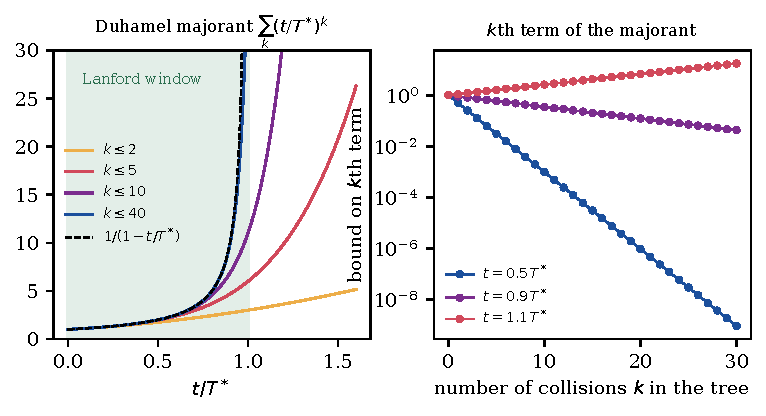
\includegraphics[width=\textwidth]{lanford_window}
\caption{Schematic of the Lanford window. Left, partial sums of the majorant $\sum_k(t/T^*)^k$ of the Duhamel series converge for $t<T^*$ (shaded) to the limit $1/(1-t/T^*)$, drawn dashed, and diverge beyond. Right, the $k$th term $(t/T^*)^k$ of the majorant, a bound on the contribution of collision trees with $k$ branchings, for $t = 0.5\,T^*$, $0.9\,T^*$ and $1.1\,T^*$: it decays geometrically inside the window and grows outside. No hard sphere quantity is computed.}
\label{fig:lanford}
\end{figure}

\subsection{Why windows cannot simply be iterated}

If chaos at time zero implies chaos at time $T^*$, why not restart the argument at $T^*$ and cover any interval by finitely many windows? The obstruction is that the conclusion of the theorem is weaker than its hypothesis. At time zero the $N$ particle law is a product measure restricted to the hard sphere phase space, with bounds in the norm $\|\cdot\|_{\beta,\gamma}$. At time $T^*$ the limit is again a product, but at finite $N$ the law carries correlations created by collisions, of size $O(\varepsilon)$ in a weak sense but not small in the norms the lemma requires, and the decay parameters have been spent: the window was obtained by trading $(\beta_0,\gamma_0)$ for $(\beta,\gamma)$, and the next window would start from worse parameters. A naive iteration therefore produces a sequence of windows whose lengths sum to a finite total.

Three ways around the obstruction are known. At equilibrium the Gibbs measure is invariant, so the a priori bounds at time $T^*$ are as good as at time zero, and many windows can be concatenated. Bodineau, Gallagher, Saint Raymond and Simonella use this invariance, for a gas in a periodic box in dimension at least three, first to show that the covariance of the fluctuations of the empirical measure is governed by the linearized Boltzmann equation globally in time, by a duality method combined with a pruning of the collision trees that removes those with superexponential growth~\cite{bgss2023cpam}, and then to show that the whole fluctuation field converges, for all times, to the solution of the fluctuating Boltzmann equation, by a study of clusters of pseudo trajectories, with quantitative bounds on time intervals that grow, slowly, with the number of particles~\cite{bgss2024}. Away from equilibrium the same authors control fluctuations and large deviations of the empirical measure, but only for short times~\cite{bgss2023}. Near equilibrium, a refinement of Lanford's argument based on estimates of the pathological collision trees gives the Brownian motion of a tagged particle of Chapter~\ref{ch:brownian}, in a diffusive limit~\cite{bgs2016}. Far from equilibrium, Deng, Hani and Ma do iterate short windows, which they call time layers, but they propagate across the layers a cumulant ansatz that records the correlations created in the earlier layers~\cite{denghanima2024}, as described after Theorem~\ref{thm:dhm}.

\subsection{Moment conditioning inside the window}

The initial data of Theorem~\ref{thm:lanford} are products restricted to non overlapping configurations, not data conditioned on moments, and what follows is a heuristic and not a theorem. A gas prepared with prescribed local density, velocity and temperature is, in the language of Chapter~\ref{ch:types}, a large system conditioned on local moments, and the conditional limit theorem suggests that its $k$ particle marginals are close to products of local Maxwellians. Lanford's theorem propagates a product structure for the length of a window, and the $H$ theorem (Theorem~\ref{thm:htheorem}) describes how the one particle law then relaxes toward the Maxwellian determined by the conserved moments. On this reading the passage from atoms to continua has three steps: conditioning on moments produces chaos, Lanford windows propagate chaos, and the Hilbert expansion of Chapter~\ref{ch:hydro} reads off the evolution of the conditioned moments as the equations of fluid dynamics. The three step picture is our framing of the subject: the first step is the heuristic above, and the second and third are Theorems~\ref{thm:lanford} and~\ref{thm:dhm} and the hydrodynamic limits of Chapter~\ref{ch:hydro}.


\section{Kac's model}

Kac~\cite{kac1956} proposed to separate the probabilistic content of Boltzmann's argument from the mechanical one by studying a Markov process whose collisions are random. Consider $N$ particles with one dimensional velocities $v = (v_1,\dots,v_N)$ on the sphere $S^{N-1}(\sqrt N) = \{\sum v_i^2 = N\}$. At rate $N$, a pair $(i,j)$ is chosen uniformly and an angle $\theta$ uniformly on $[0,2\pi)$, and the pair is rotated:
\[
(v_i,v_j)\mapsto(v_i\cos\theta-v_j\sin\theta,\;v_i\sin\theta+v_j\cos\theta).
\]
Energy is conserved, momentum is not. The uniform measure on the sphere is invariant and, by the Maxwell, Poincar\'e and Borel lemma (Theorem~\ref{thm:sphere_lemma}), its one particle marginal converges to the standard Gaussian. The generator acts on symmetric functions, and the master equation for the law $F_N(t)$ is linear.

\begin{theorem}[Kac]
\label{thm:kac}
If $F_N(0)$ is $f_0$ chaotic in the sense of Chapter~\ref{ch:axioms}, then $F_N(t)$ is $f_t$ chaotic for every $t>0$, where $f_t$ solves the Kac Boltzmann equation
\[
\partial_tf(v) = \frac{1}{\pi}\int_{\R}\int_0^{2\pi}\big(f(v')f(w')-f(v)f(w)\big)\dd\theta\dd w,
\]
with $(v',w')$ the rotation of $(v,w)$ by $\theta$.
\end{theorem}

Kac proved the theorem~\cite{kac1956} by expanding the evolution in a power series in time, where the combinatorics of the Markov generator replace the geometry of collisions; the stochasticity removes recollisions as an issue. We quote the theorem without proof. Figure~\ref{fig:kac} shows a simulation started from a bimodal law: the one particle histogram relaxes to the Gaussian and the kurtosis, which is about $1.04$ for the initial law, approaches three. The decay is consistent with the linear recursion for the fourth moment: a single collision maps $m_4$ to $\frac34m_4+\frac34$ when $m_2 = 1$, whose fixed point is the Gaussian value three.

\begin{figure}[t]
\centering
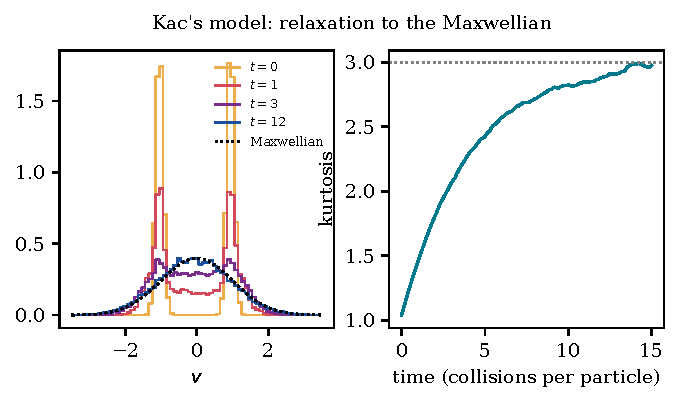
\includegraphics[width=\textwidth]{kac_model}
\caption{Kac's model with $N=20{,}000$ particles. The initial law is an equal mixture of two Gaussian peaks at $\pm1$ with standard deviation $0.1$, scaled to unit second moment. Left, one particle histograms at times $0$, $1$, $3$ and $12$, measured in collisions per particle, with the Maxwellian dotted; right, kurtosis against the same time, with the Gaussian value three dotted.}
\label{fig:kac}
\end{figure}

Kac also proposed a program: prove convergence to equilibrium for the $N$ particle process uniformly in $N$, and deduce convergence for the Boltzmann equation. The spectral gap of the generator is bounded below uniformly in $N$, as shown by Janvresse~\cite{janvresse2001} and computed exactly by Carlen, Carvalho and Loss~\cite{ccl2003}, so the $L^2$ part of the program works. But $L^2$ is the wrong norm, since chaotic densities have $L^2$ norms exponential in $N$; the right quantity is relative entropy, which is extensive, and the entropy production of the $N$ particle process does not control entropy uniformly in $N$. The largest constant $\Gamma_N$ such that the entropy production is at least $\Gamma_N$ times the relative entropy with respect to the uniform law on the sphere, for every initial law of finite relative entropy, is at least $2/(N-1)$ by an argument of Villani~\cite{villani2003cercignani} and tends to zero as $N\to\infty$~\cite{cclv2010}. Gao, Wang and Xia~\cite{gaowangxia2026} prove in a recent preprint that $\Gamma_N = 2/(N-1)$ for every $N\geq2$, which confirms Villani's conjecture that $\Gamma_N$ is of order $1/N$; Open Problem~\ref{prob:kinetic} of Chapter~\ref{ch:open} asks for classes of initial laws on which a constant independent of $N$ exists. Mischler and Mouhot~\cite{mischlermouhot2013} completed a quantitative version of Kac's program, proving propagation of chaos with explicit rates in Wasserstein distance uniformly in time.

\section{Propagation of chaos for mean field diffusions}

A clean case in which propagation of chaos can be proved in a few lines is the mean field diffusion. Let $b:\R^d\times\R^d\to\R^d$ be Lipschitz with constant $L$, in the sense that $|b(x,y)-b(x',y')|\leq L(|x-x'|+|y-y'|)$, and consider
\[
\dd X^i_t = \frac1N\sum_{j=1}^Nb(X^i_t,X^j_t)\dd t+\dd W^i_t,\qquad i = 1,\dots,N,
\]
with independent Brownian motions and independent initial conditions of law $f_0$. The candidate limit is the McKean Vlasov process
\[
\dd\bar X^i_t = \int b(\bar X^i_t,y)\,f_t(\dd y)\dd t+\dd W^i_t,\qquad f_t = \mathrm{Law}(\bar X^i_t),
\]
driven by the same Brownian motion and started at the same point. For Lipschitz $b$ and $\E|X^i_0|^2<\infty$ the McKean Vlasov equation has a unique solution~\cite{sznitman1991}, and the $\bar X^i$ are independent and identically distributed. The coupling argument below is due to Sznitman~\cite{sznitman1991}. It is a different result from Theorem~\ref{thm:sznitman}, from the same lectures, which relates chaos to the convergence of empirical measures.

\begin{theorem}[McKean Vlasov coupling]
\label{thm:mckean}
Assume that $\E|X^i_0|^2<\infty$. For every $T$ there is $C_T$, depending only on $L$, $T$, $d$ and $\E|X^i_0-\E X^i_0|^2$, such that
\[
\sup_{t\leq T}\E|X^i_t-\bar X^i_t|\leq\frac{C_T}{\sqrt N}.
\]
Consequently the $k$ particle marginals of $(X^1_t,\dots,X^N_t)$ converge to $f_t^{\otimes k}$ in the Wasserstein distance $W_1$ for the metric $\sum_{i\leq k}|x_i-y_i|$, uniformly in $t\leq T$ and at rate $kC_T/\sqrt N$.
\end{theorem}

\begin{proof}
Subtracting the equations,
\[
|X^i_t-\bar X^i_t|\leq\int_0^t\Big|\frac1N\sum_jb(X^i_s,X^j_s)-\int b(\bar X^i_s,y)f_s(\dd y)\Big|\dd s.
\]
Insert $\frac1N\sum_jb(\bar X^i_s,\bar X^j_s)$. The Lipschitz bound controls the first difference by $\frac{L}{N}\sum_j(|X^i_s-\bar X^i_s|+|X^j_s-\bar X^j_s|)$, whose expectation is $2L\,\E|X^1_s-\bar X^1_s|$ by exchangeability. The second difference is an average of $N$ terms $b(\bar X^i_s,\bar X^j_s)-\int b(\bar X^i_s,y)f_s(\dd y)$. Put $V_T = \sup_{s\leq T}\E|\bar X^1_s-\E\bar X^1_s|^2$. For $j\neq i$ the terms are, conditionally on $\bar X^i_s$, centered and independent, with conditional variance at most $L^2V_T$; the term $j = i$ is at most $L\int|\bar X^i_s-y|f_s(\dd y)$ in absolute value, which has mean at most $L\sqrt{2V_T}$. By the Cauchy Schwarz inequality the mean absolute value of the second difference is at most $(1+\sqrt2)L\sqrt{V_T/N}\leq3L\sqrt{V_T/N}$. Hence $\psi(t) = \E|X^1_t-\bar X^1_t|$ satisfies $\psi(t)\leq\int_0^t\big(2L\psi(s)+3L\sqrt{V_T/N}\big)\dd s$, and Gr\"onwall's lemma gives $\psi(t)\leq\frac32\sqrt{V_T/N}\,(e^{2Lt}-1)$.

It remains to bound $V_T$, and this is where the second moment of $f_0$ enters. Let $\bar X$ and $\bar X'$ be independent copies of the McKean Vlasov process, with Brownian motions $W$ and $W'$, and $D = \bar X-\bar X'$. The drift $x\mapsto\int b(x,y)f_s(\dd y)$ is $L$ Lipschitz, so $|D_s|\leq|D_0|+\sup_{r\leq s}|W_r-W'_r|+L\int_0^s|D_r|\dd r$. Gr\"onwall's lemma and Doob's inequality give $\E|D_s|^2\leq2e^{2Ls}(2v_0+8ds)$ with $v_0 = \E|X^i_0-\E X^i_0|^2$, and $\E|\bar X_s-\E\bar X_s|^2 = \frac12\E|D_s|^2$, so $V_T\leq e^{2LT}(2v_0+8dT)$. Replacing $V_T$ by this bound in the estimate of $\psi$ gives the theorem with $C_T = \frac32\sqrt{e^{2LT}(2v_0+8dT)}\,(e^{2LT}-1)$, which depends only on $L$, $T$, $d$ and $v_0$.
\end{proof}

The coupling proof is the simplest instance of a principle that runs through this book. A many particle system is compared with $N$ independent copies of a nonlinear one particle process; the comparison is a law of large numbers for the empirical measure, and the error is the fluctuation, of order $N^{-1/2}$. The same structure governs particle filters, ensemble Kalman filters and the particle approximations of generative flows in Part~\ref{part:statmech}.

\section{The arrow of time: Kac's ring}

Kac devised an exactly solvable model in which both Boltzmann's prediction and its failure can be seen~\cite{kac1959}. Place $N$ sites on a circle, each holding a ball that is white or black. A fixed subset of $m$ edges between adjacent sites is marked. At each time step every ball moves one site clockwise, and a ball crossing a marked edge changes color. Let $N^w_t$ and $N^b_t$ be the numbers of white and black balls. Boltzmann's reasoning, which assumes that the color of the ball about to cross an edge is independent of whether the edge is marked, the analogue of the \emph{Stosszahlansatz}, predicts with $\mu = m/N$
\begin{gather*}
N^w_{t+1}-N^b_{t+1} = (1-2\mu)(N^w_t-N^b_t), \\
\frac{N^w_t-N^b_t}{N} = (1-2\mu)^t\,\frac{N^w_0-N^b_0}{N},
\end{gather*}
exponential relaxation to equal numbers of each color. But the dynamics is deterministic and reversible, and after $2N$ steps every ball has crossed every edge twice, so the configuration returns exactly: the recurrence time is $2N$, and after $N$ steps every ball has crossed all $m$ marked edges once, so if $m$ is odd the colors are exactly reversed.

Figure~\ref{fig:kacring} shows the model: for $t$ much smaller than $N$ the trajectory follows Boltzmann's prediction closely. Kac showed that if the marked set is chosen at random, Boltzmann's prediction holds for most marked sets, for each fixed $t$, as $N\to\infty$: the fluctuations of $(N^w_t-N^b_t)/N$ about $(1-2\mu)^t$ are of order $N^{-1/2}$. The arrow of time is a law of large numbers over the disorder, valid for times small compared with the recurrence time. This is precisely the structure of Lanford's theorem, and the content of Boltzmann's reply to Zermelo.

\begin{figure}[t]
\centering
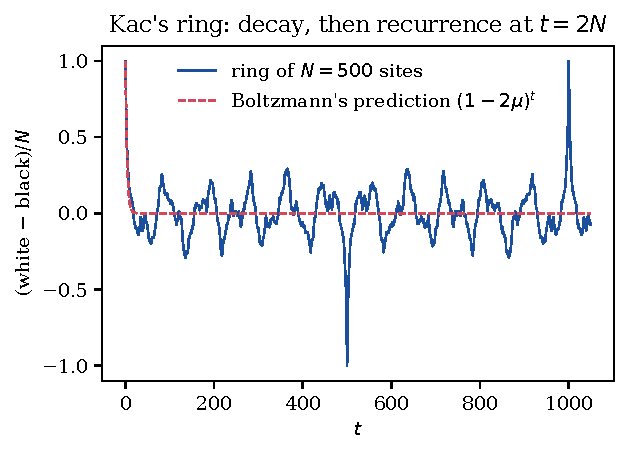
\includegraphics[width=0.92\textwidth]{kac_ring}
\caption{Kac's ring with $N=500$ sites and $61$ marked edges, started with all balls white. The deterministic dynamics follows Boltzmann's exponential law, then reverses at $t=N$ and recurs at $t=2N$.}
\label{fig:kacring}
\end{figure}

\section{Ergodic theorems}

The other classical route to justifying averages is ergodic theory. Its basic results, Birkhoff's pointwise ergodic theorem (Theorem~\ref{thm:birkhoff}) and von Neumann's mean ergodic theorem (Theorem~\ref{thm:vonneumann}), are proved in Chapter~\ref{ch:ergodic}.

Sinai proved in 1970~\cite{sinai1970} that dispersing billiards are ergodic, and Sim\'anyi proved the Boltzmann Sinai ergodic hypothesis for hard ball systems on tori in stages: for typical hard disk systems in 2003~\cite{simanyi2003}, for typical hard ball systems in 2004~\cite{simanyi2004}, in general under a technical assumption in 2009~\cite{simanyi2009}, and without that assumption in 2013~\cite{simanyi2013}. Ergodicity, however, is the wrong tool for the sixth problem. It speaks about time averages of a single system over times comparable to recurrence times, while the kinetic limit concerns ensemble averages over times of order the mean free time, for typical initial conditions, as the number of particles diverges. Lanford's theorem uses no ergodic theory. In the language of Chapter~\ref{ch:axioms}, it is a statement about the de Finetti measure of the gas, and its probabilistic content is that independence, once assumed, propagates.

\section{The Lorentz gas: a derivation valid for all times}

There is one kinetic limit in which the restriction to short times disappears. In the Lorentz gas a single particle moves among fixed spherical scatterers of radius $\varepsilon$ placed at the points of a Poisson process of intensity $\varepsilon^{-(d-1)}$, reflecting elastically. Gallavotti showed in 1969~\cite{gallavotti1969}, and Spohn~\cite{spohn1978} and Boldrighini, Bunimovich and Sinai~\cite{bbs1983} extended the result, that in the Boltzmann Grad limit the law of the particle, averaged over the scatterers, converges for all times to the solution of the linear Boltzmann equation
\[
\partial_tf+v\cdot\nabla_xf = \int_{S^{d-1}}\big(f(v')-f(v)\big)\,|v|\,b(\omega)\dd\omega.
\]
The linear equation describes a particle whose velocity jumps at the times of a Poisson process, a Markov process in phase space. The difficulty of Lanford's theorem, recollisions between moving particles, is replaced by the possibility of returning to a scatterer already visited, and since the scatterers are Poisson distributed and the particle explores new territory, such returns have vanishing probability on every bounded time interval. The theorem shows that the Markov property, the essence of Boltzmann's assumption, emerges from deterministic dynamics in a random medium. Averaging over the medium is a de Finetti average, and the Poisson law of the scatterers is the prior that makes the limit Markov.

For a periodic arrangement of scatterers the result fails: Golse~\cite{golse2008} showed that the limit is not described by the linear Boltzmann equation, and Marklof and Str\"ombergsson~\cite{marklof2011} identified the correct limit, a generalized kinetic equation with memory, using ergodic theory on homogeneous spaces. The randomness of the medium matters, which is another form of Poincar\'e's observation that the irreversible limit is a statement about a probability measure on initial conditions.

\section{Mean field limits and the Vlasov equation}

When the interaction is long range and weak rather than short range and strong, the kinetic limit is the Vlasov equation
\[
\partial_tf+v\cdot\nabla_xf-(\nabla W*\rho_f)\cdot\nabla_vf = 0,\qquad\rho_f = \int f\dd v,
\]
for particles interacting through a potential $W$ scaled by $1/N$. Braun and Hepp in 1977~\cite{braunhepp1977} and Dobrushin in 1979~\cite{dobrushin1979} proved the mean field limit for smooth $W$ by a stability estimate in Wasserstein distance: two solutions of the Vlasov equation, and in particular an empirical measure of the $N$ particle system and the true solution, separate at most exponentially in time in $W_1$. Dobrushin's estimate is the deterministic counterpart of the coupling argument of Theorem~\ref{thm:mckean}. The singular case of the Coulomb interaction, relevant to plasmas and galaxies, was long out of reach; the modulated energy method of Serfaty~\cite{serfaty2020} gives mean field limits for Coulomb and Riesz interactions, for gradient and conservative first order flows and, for Newton's law, in the monokinetic case. The Vlasov equation is reversible, and its long time behavior, Landau damping, is a mixing phenomenon in velocity space proved in the nonlinear setting by Mouhot and Villani~\cite{mouhotvillani2011}. It is a second route to irreversibility, through phase mixing rather than collisions.

\section{Grad's moment method and the closure problem}

Integrating the Boltzmann equation against polynomials in $v$ yields an infinite hierarchy of moment equations, each involving the next. Grad's thirteen moment method of 1949~\cite{grad1949} closes the hierarchy by assuming that $f$ is a local Maxwellian times a polynomial of degree three determined by thirteen moments: density, velocity, temperature, stress and heat flux. The resulting hyperbolic system reproduces Navier Stokes Fourier in the hydrodynamic limit and extends it into the transition regime, but it can lose hyperbolicity and produce unphysical shocks. Levermore's maximum entropy closures~\cite{levermore1996} replace the polynomial ansatz by the density maximizing entropy subject to the moment constraints, an exponential family, which guarantees hyperbolicity and an entropy inequality at the cost of nonpolynomial fluxes. Closure problems in kinetic theory, in turbulence modeling and in approximate Bayesian inference, where variational families play the role of the closure ansatz, are versions of the same question: which low dimensional family best represents a high dimensional law consistent with known averages.

\section*{Exercises}
\begin{enumerate}
\item Verify that the pre and post collisional change of variables in Lemma~\ref{lem:weakform} has unit Jacobian.
\item For Kac's model, derive the differential equation satisfied by the fourth moment under the normalization of Theorem~\ref{thm:kac}, and solve it.
\item In Kac's ring with $N$ sites and $m$ marked edges, show that the configuration at time $N$ is the color reversal of the initial one when $m$ is odd and equal to it when $m$ is even.
\item In dimension one, take $b(x,y) = Ly$ and $f_0 = N(0,s^2)$ in Theorem~\ref{thm:mckean}. Compute $\E|X^i_t-\bar X^i_t|$ exactly and show that it is at least $\sqrt{2/\pi}\,(e^{Lt}-1)s/\sqrt N$, so that $C_T$ must depend on the variance of $f_0$.
\item Show that the linear Boltzmann equation conserves mass and kinetic energy but not momentum, and identify its equilibria.
\end{enumerate}


\section*{Notes}

Cercignani, Illner and Pulvirenti~\cite{cip1994} is the classical text on the mathematical theory of dilute gases. Villani's review~\cite{villani2002review} is the standard survey of the mathematics of the Boltzmann equation. Gallagher's article in the Bulletin~\cite{gallagher2019} explains the passage from Newton to Navier Stokes, and the Bourbaki expos\'e of Bodineau, Gallagher, Saint Raymond and Simonella~\cite{bgss2026} explains the proof of Deng, Hani and Ma.

\chapter{From Boltzmann to Navier Stokes}
\label{ch:hydro}

\section{Hilbert's expansion}

The second limit in Hilbert's sentence, from the kinetic description to the laws of continua, was the one Hilbert himself attacked. In his 1912 paper~\cite{hilbert1912} he introduced a small parameter $\varepsilon$, the ratio of the mean free path to the macroscopic length, now called the Knudsen number, wrote the Boltzmann equation as
\[
\partial_tf_\varepsilon+v\cdot\nabla_xf_\varepsilon = \frac1\varepsilon Q(f_\varepsilon,f_\varepsilon),
\]
and sought a solution as a formal power series $f_\varepsilon = f_0+\varepsilon f_1+\varepsilon^2f_2+\cdots$. At order $\varepsilon^{-1}$ one finds $Q(f_0,f_0) = 0$, so $f_0$ is a local Maxwellian whose density, velocity and temperature depend on $(t,x)$. At each subsequent order one must solve a linear equation $\mathcal{L}f_{k+1} = (\text{known})$, where $\mathcal{L}$ is the collision operator linearized at $f_0$. Hilbert proved, using his theory of integral equations, that $\mathcal{L}$ satisfies a Fredholm alternative: the equation is solvable if and only if the right side is orthogonal to the collision invariants, and the solvability conditions are the equations of fluid dynamics. This was one of the first applications of Hilbert space methods to a problem of physics, and it showed that Hilbert regarded his sixth problem as a problem of analysis.

Chapman in 1916~\cite{chapman1916} and Enskog in 1917~\cite{enskog1917} reorganized the expansion so that the fluid variables are not expanded but remain exact, which avoids secular growth and yields at successive orders the Euler equations, the Navier Stokes equations with explicit transport coefficients, and the Burnett equations. For the dilute noble gases the Chapman Enskog formulas, with realistic pair potentials fitted to experimental data, reproduce the measured viscosity and heat conductivity to within one percent between 50 and 1000 K~\cite{kestin1984}.

\section{The Euler limit}

Let $M_{\rho,u,\theta}(v) = \rho(2\pi\theta)^{-d/2}\exp(-|v-u|^2/2\theta)$. Its moments are
\begin{gather*}
\int M = \rho,\quad\int vM = \rho u,\quad\int v\otimes vM = \rho u\otimes u+\rho\theta I,\\ \int\tfrac12|v|^2vM = \Big(\tfrac12\rho|u|^2+\tfrac{d+2}{2}\rho\theta\Big)u.
\end{gather*}
Integrating the Boltzmann equation against the collision invariants $1$, $v$ and $\frac12|v|^2$, the collision term drops out by Lemma~\ref{lem:weakform}, and we obtain local conservation laws for mass, momentum and energy whose fluxes are moments of $f$. If $f$ is replaced by the local Maxwellian with the same $(\rho,u,\theta)$, the fluxes are those just computed and the conservation laws become the compressible Euler equations
\begin{align*}
\partial_t\rho+\nabla\cdot(\rho u) &= 0,\\
\partial_t(\rho u)+\nabla\cdot(\rho u\otimes u)+\nabla p &= 0,\\
\partial_tE+\nabla\cdot\big((E+p)u\big) &= 0,
\end{align*}
with pressure $p = \rho\theta$ and energy $E = \frac12\rho|u|^2+\frac d2\rho\theta$, the equation of state of a monatomic ideal gas. \begin{theorem}[Caflisch]
\label{thm:caflisch}
Let $(\rho,u,\theta)$ be a smooth solution of the compressible Euler equations on $[0,T]$ in one space dimension with periodic boundary conditions, with $\rho,\theta$ bounded away from zero. For hard sphere collisions and $\varepsilon$ small enough, there is a solution $f_\varepsilon$ of the Boltzmann equation with Knudsen number $\varepsilon$ on $[0,T]$ such that
\[
\sup_{t\leq T}\big\|f_\varepsilon(t)-M_{\rho(t),u(t),\theta(t)}\big\|_{H^1_{x,v}}\leq C\varepsilon.
\]
The solution is the truncated Hilbert expansion $f_\varepsilon = \sum_{n=0}^6\varepsilon^nf_n+\varepsilon^3f_{R,\varepsilon}$ with $f_{R,\varepsilon}(0) = 0$, so its initial datum is the expansion at time zero.
\end{theorem}

The theorem makes the Euler limit rigorous on the time interval of smooth Euler flow, which for generic data is finite because of shock formation. We quote the theorem without proof. Caflisch~\cite{caflisch1980} proves it for hard cutoff potentials in the sense of Grad, states that an Euler solution in $H^9$ suffices, and remarks that the same method treats several space dimensions. Guo, Jang and Jiang~\cite{guojangjiang2009} gave a new proof on $\R^3$ and on the three dimensional torus, by an $L^2$ to $L^\infty$ method that does not require $f_{R,\varepsilon}(0) = 0$, under the assumption that the temperature of the Euler solution varies by less than a factor of two. The remainder is controlled by the spectral gap of the linearized operator, so the argument is a Poincar\'e inequality in disguise.

\section{The linearized operator}

Fix the standard Maxwellian $M(v) = (2\pi)^{-d/2}e^{-|v|^2/2}$ and write $f = M(1+g)$. The linearized operator is
\[
\mathcal{L}g = -\frac1M\big(Q(M,Mg)+Q(Mg,M)\big),
\]
acting on $L^2(M\dd v)$, where $Q(f,h) = \iint B\,(f'h'_*-fh_*)\dd\sigma\dd v_*$ is the bilinear collision operator, so that $Q(f,f)$ is the operator of Chapter~\ref{ch:kinetic}.

\begin{theorem}[Hilbert, Grad]
\label{thm:linearized}
For hard spheres, $\mathcal{L}$ is a nonnegative self adjoint operator on $L^2(M\dd v)$ with kernel spanned by $1,v_1,\dots,v_d,|v|^2$. It has the form $\mathcal{L} = \nu_c(v)-K$, where the collision frequency $\nu_c(v)$ grows like $1+|v|$ and $K$ is compact. In particular $\mathcal{L}$ satisfies a Fredholm alternative on the orthogonal complement of its kernel and has a spectral gap there in the weighted sense.
\end{theorem}

Nonnegativity and symmetry follow from the two symmetries used in the proof of Lemma~\ref{lem:weakform}. Since $M'M'_* = MM_*$, the definition gives $\mathcal{L}g = -\iint B\,M_*\big(g'+g'_*-g-g_*\big)\dd\sigma\dd v_*$, and the swap of $v$ and $v_*$ followed by the pre and post collisional change of variables gives, for $\varphi$ and $g$ for which the integrals converge,
\[
\begin{aligned}\langle\varphi,\mathcal{L}g\rangle_{L^2(M)} &= \frac14\iiint B\,MM_*\big(\varphi'+\varphi'_*-\varphi-\varphi_*\big)\\ &\qquad\times\big(g'+g'_*-g-g_*\big)\dd\sigma\dd v_*\dd v.\end{aligned}
\]
The right side is symmetric in $\varphi$ and $g$, and for $\varphi = g$ it is nonnegative. Self adjointness of $\mathcal{L}$ itself follows from the splitting $\mathcal{L} = \nu_c-K$, in which $\nu_c$ is multiplication by a positive function and $K$ is bounded and, by the symmetry of the form, symmetric. The kernel is identified by Lemma~\ref{lem:collision_invariants}. We quote the splitting, the growth of $\nu_c$, the compactness of $K$, the Fredholm alternative and the spectral gap without proof. Compactness of $K$ is Hilbert's contribution of 1912~\cite{hilbert1912}; Grad extended the analysis to a large class of kernels in 1963~\cite{grad1963}.

\section{The incompressible Navier Stokes limit}

The Euler limit loses dissipation. To see viscosity one must look at fluctuations about a global equilibrium on a diffusive time scale. Bardos, Golse and Levermore~\cite{bgl1991} identified the scaling:
\begin{equation}
\varepsilon\,\partial_tf_\varepsilon+v\cdot\nabla_xf_\varepsilon = \frac1\varepsilon Q(f_\varepsilon,f_\varepsilon),\qquad f_\varepsilon = M(1+\varepsilon g_\varepsilon).
\label{eq:bgl_scaling}
\end{equation}
Time is slow compared with the transport time, the Mach number is of order $\varepsilon$, and the Knudsen number is $\varepsilon$, so the Reynolds number, by von K\'arm\'an's relation, is of order one. Substituting, $g_\varepsilon$ solves
\[
\varepsilon\,\partial_tg_\varepsilon+v\cdot\nabla_xg_\varepsilon+\frac1\varepsilon\mathcal{L}g_\varepsilon = \Gamma(g_\varepsilon,g_\varepsilon),
\]
where $\Gamma(g,g) = M^{-1}Q(Mg,Mg)$ is the quadratic part.

\begin{theorem}[Formal limit, Bardos, Golse and Levermore]
\label{thm:bgl}
Suppose $g_\varepsilon\to g$ in a sense strong enough to pass to the limit in the equation. Then
\[
g(t,x,v) = \rho(t,x)+u(t,x)\cdot v+\theta(t,x)\frac{|v|^2-d}{2},
\]
with $\nabla\cdot u = 0$ and $\nabla(\rho+\theta) = 0$, and $(u,\theta)$ solve the incompressible Navier Stokes Fourier system
\begin{align*}
\partial_tu+u\cdot\nabla u+\nabla p &= \nu\Delta u,\\
\partial_t\theta+u\cdot\nabla\theta &= \kappa\Delta\theta,
\end{align*}
with transport coefficients
\[
\nu = \frac{1}{(d-1)(d+2)}\int\hat A:A\,M\dd v,\qquad\kappa = \frac{2}{d(d+2)}\int\hat B\cdot B\,M\dd v,
\]
where $A(v) = v\otimes v-\frac{|v|^2}{d}I$, $B(v) = \frac12v(|v|^2-(d+2))$, and $\hat A$, $\hat B$ are the unique solutions orthogonal to the kernel of $\mathcal{L}\hat A = A$ and $\mathcal{L}\hat B = B$.
\end{theorem}

\begin{proof}[Derivation]
Multiplying the equation for $g_\varepsilon$ by $\varepsilon$ and letting $\varepsilon\to0$ gives $\mathcal{L}g = 0$, so $g$ lies in the kernel and has the stated form. Taking moments of the equation against $\varphi = 1$, $v$ and $|v|^2$, for which the collision terms vanish, gives conservation laws of the form $\varepsilon\,\partial_t\int\varphi\,g_\varepsilon M\dd v+\nabla_x\cdot\int v\varphi\,g_\varepsilon M\dd v = 0$. For $g$ of the stated form, $\int v\,gM\dd v = u$ and $\int v\otimes v\,gM\dd v = (\rho+\theta)I$, so letting $\varepsilon\to0$ gives at leading order $\nabla\cdot u = 0$ and $\nabla(\rho+\theta) = 0$, the incompressibility and Boussinesq relations. Dividing the conservation laws by $\varepsilon$, the next order needs the momentum and energy fluxes, $\frac1\varepsilon\int A\,g_\varepsilon M$ and $\frac1\varepsilon\int Bg_\varepsilon M$. Since $A$ and $B$ are orthogonal to the kernel, $\frac1\varepsilon\int Ag_\varepsilon M = \frac1\varepsilon\langle\mathcal{L}\hat A,g_\varepsilon\rangle = \frac1\varepsilon\langle\hat A,\mathcal{L}g_\varepsilon\rangle$, and the equation gives $\frac1\varepsilon\mathcal{L}g_\varepsilon = \Gamma(g_\varepsilon,g_\varepsilon)-v\cdot\nabla_xg_\varepsilon+O(\varepsilon)$. Substituting the limit form of $g$, the quadratic term produces the convection $u\cdot\nabla u$ and the transport term produces $-\nu\,(\nabla u+\nabla u^\top)$, using the rotational invariance of $\mathcal{L}$, which forces $\hat A(v) = a(|v|)A(v)$ and reduces $\int\hat A_{ij}A_{kl}M$ to a multiple of the isotropic fourth order tensor. Taking the divergence and using $\nabla\cdot u = 0$ yields $\nu\Delta u$. The energy equation is obtained in the same way with $B$ in place of $A$, the factor $\frac{d+2}{2}$ in front of $\partial_t\theta+u\cdot\nabla\theta$ being absorbed in $\kappa$.
\end{proof}

Since $\mathcal{L}$ commutes with rotations of velocity space and $A$ is a traceless symmetric tensor, $\hat A(v) = a(|v|)A(v)$ for a scalar function $a$, and the fourth order tensor $T_{ijkl} = \int\hat A_{ij}A_{kl}M\dd v$ is isotropic, symmetric and traceless in each pair of indices. The only such tensor is a multiple of
\[
\frac12\big(\delta_{ik}\delta_{jl}+\delta_{il}\delta_{jk}\big)-\frac1d\delta_{ij}\delta_{kl},
\]
and contracting over $i = k$, $j = l$ identifies the multiple as $2\int\hat A:A\,M/((d-1)(d+2))$, which is $2\nu$. Hence for any velocity gradient, $\int\hat A_{ij}\,(v\cdot\nabla)(u\cdot v)\,M\dd v = \partial_ku_l\,T_{ijkl} = \nu\big(\partial_iu_j+\partial_ju_i-\frac2d(\nabla\cdot u)\delta_{ij}\big)$, where we used $v_kv_l = A_{kl}+\frac1d|v|^2\delta_{kl}$ and the orthogonality of $\hat A$ to the isotropic part. The theorem shows that the viscosity of a gas is a Green Kubo type coefficient: an inner product of a flux with the inverse of the linearized collision operator applied to the same flux. For hard spheres it can be computed numerically to high accuracy and agrees with Chapman and Enskog. Golse and Saint Raymond~\cite{golsesaintraymond2004} made the derivation rigorous for bounded collision kernels, a class that excludes hard spheres: renormalized solutions of the Boltzmann equation on $\R^3$ in the scaling \eqref{eq:bgl_scaling}, which exist globally by DiPerna and Lions~\cite{diperna1989}, have fluctuations whose limit points are Leray solutions of the Navier Stokes Fourier system. The same authors extended the Navier Stokes limit to hard cutoff potentials, which include hard spheres~\cite{golsesaintraymond2009}, and Levermore and Masmoudi~\cite{levermoremasmoudi2010} proved the Navier Stokes Fourier limit on periodic domains of dimension two or more for a still wider class of kernels.

\section{Hydrodynamic limits from stochastic particle systems}
\label{sec:particle_hydro}

A second route from particles to continua bypasses the Boltzmann equation and starts from stochastic interacting particle systems, where the noise does the work that molecular chaos does in Lanford's theorem. The simplest case can be done completely.

The symmetric simple exclusion process on the discrete torus $\T_N = \Z/N\Z$ has configurations $\eta\in\{0,1\}^{\T_N}$; each particle attempts to jump to each neighbor at rate one, and the jump succeeds if the target is empty. Equivalently, the contents of each pair of adjacent sites are exchanged at rate one. The generator is
\[
\mathcal{A}F(\eta) = \sum_{x\in\T_N}\big(F(\eta^{x,x+1})-F(\eta)\big),
\]
where $\eta^{x,x+1}$ exchanges the occupations of $x$ and $x+1$.

\begin{theorem}[Hydrodynamic limit for simple exclusion]
\label{thm:ssep}
Let $\rho_0:\T\to[0,1]$ be continuous, where $\T = \R/\Z$ is the circle of length one, and start the process from the product measure with $\P(\eta_0(x) = 1) = \rho_0(x/N)$. Speed up time by $N^2$. For every continuous $G:\T\to\R$ and $t\geq0$,
\[
\frac1N\sum_{x\in\T_N}G\Big(\frac xN\Big)\eta_{N^2t}(x)\longrightarrow\int_\T G(u)\rho(t,u)\dd u\quad\text{in probability},
\]
where $\rho$ solves the heat equation $\partial_t\rho = \partial_u^2\rho$ with $\rho(0,\cdot) = \rho_0$.
\end{theorem}

\begin{proof}
Applying the generator to $F(\eta) = \eta(x)$ gives $\mathcal{A}\eta(x) = \eta(x+1)+\eta(x-1)-2\eta(x)$, a discrete Laplacian. Hence $m_t(x) = \E\eta_t(x)$ solves the closed linear system $\partial_tm = \Delta_Nm$, whose solution is $m_t(x) = \sum_yp_t(x,y)\rho_0(y/N)$ with $p_t$ the transition kernel of a continuous time simple random walk jumping at rate one to each neighbor. Under the diffusive scaling, $p_{N^2t}$ converges to the heat kernel by the local central limit theorem, so the mean of the empirical average converges to $\int G\rho(t)$. For the variance, the exclusion process started from a product measure has nonpositive two point correlations, $\E[\eta_t(x)\eta_t(y)]\leq m_t(x)m_t(y)$ for $x\neq y$, a consequence of Liggett's correlation inequality for exclusion processes~\cite{liggett1985}. For $G\geq0$ the covariance terms are therefore nonpositive, and
\[
\begin{aligned}\Var\Big(\frac1N\sum_xG(x/N)\eta_t(x)\Big)&\leq\frac{1}{N^2}\sum_xG(x/N)^2\,m_t(x)(1-m_t(x))\\ &\leq\frac{\|G\|_\infty^2}{4N}.\end{aligned}
\]
For general $G$ write $G = G^+-G^-$ and use $\Var(S^+-S^-)\leq2\Var(S^+)+2\Var(S^-)$, which gives the bound $\|G\|_\infty^2/N$; Chebyshev's inequality completes the proof.
\end{proof}

The closure of the first moment equation is an exact duality: the expectation of one occupation variable is governed by a single random walk. For general interacting systems no such closure exists, and Guo, Papanicolaou and Varadhan~\cite{gpv1988} developed the entropy method, which proves the hydrodynamic limit for gradient systems by controlling the relative entropy of the process with respect to local equilibria and replacing microscopic currents by functions of the local density through the one and two block estimates. Yau's relative entropy method of 1991~\cite{yau1991} gives a cleaner proof when the limit is smooth. Large deviations from the hydrodynamic limit, the theory of Kipnis, Olla and Varadhan~\cite{kipnis1989} and its macroscopic fluctuation extension by Bertini, De Sole, Gabrielli, Jona Lasinio and Landim~\cite{bertini2015}, show that the probability of observing an atypical macroscopic evolution is exponentially small in the number of particles with a rate given by an action functional. This is the Sanov theorem of hydrodynamics, and it is the bridge to the inferential reading: conditioning on an atypical macroscopic observation, the most likely microscopic history is the minimizer of that action, which is Schr\"odinger's question of Chapter~\ref{ch:quantum} in a new setting.

\section{The full derivation}

Deng, Hani and Ma~\cite{denghanima2025} combine their long time derivation of the Boltzmann equation, Theorem~\ref{thm:dhm}, with hydrodynamic limits of the kind described above, and derive fluid equations from hard sphere dynamics. The setting is the torus in dimension two or three. The incompressible Navier Stokes Fourier system is obtained for smooth solutions near global equilibrium, from the result of Gallagher and Tristani~\cite{gallaghertristani2020}, and the compressible Euler system for a smooth solution on a fixed time interval, from the Hilbert expansion of Theorem~\ref{thm:caflisch} in the form of Guo, Jang and Jiang~\cite{guojangjiang2009}. The Knudsen number tends to zero while the number of particles diverges in the Boltzmann Grad scaling, either in two steps, the kinetic limit at a fixed Knudsen number and then the Knudsen number to zero, or jointly, and in the joint limit the Knudsen number must tend to zero slowly enough that the kinetic approximation remains valid on the hydrodynamic time scale. In their notation the particle diameter is $\varepsilon$ and the Knudsen number is $\delta$, and for a smooth fluid solution on $[0,T]$ the joint limit requires $\max(1,\delta^{-1})\max(1,\delta^{-1}T)\ll(\log\log(1/\varepsilon))^{1/2}$. This required the long time theorem in an essential way: Lanford's time is a fixed fraction of the kinetic time and therefore vanishes on the hydrodynamic scale. Deng, Hani and Ma state that the result resolves Hilbert's sixth problem as it pertains to the program of deriving the fluid equations from Newton's laws by way of Boltzmann's kinetic theory, for the hard sphere model on the torus and for as long as the limiting fluid equations have smooth solutions.

\section{What the derivation does not give}

Three limitations of the derivational reading are worth stating, because each is the starting point of a later chapter.

First, the derivation is conditional on the regularity of the limit. In three dimensions it is unknown whether smooth solutions of the Navier Stokes equations remain smooth for all time, the Clay Millennium problem. Chapter~\ref{ch:boundary} discusses blowup and turbulence as phenomena at the boundary of the derivation.

Second, the derivation assumes the initial state is a chaotic law, a product of one particle densities that are themselves close to a local Maxwellian. Real flows are observed, not prescribed. The question of which microscopic states are compatible with a given macroscopic observation, and with what probabilities, is the inferential problem, and Theorem~\ref{thm:gibbs_conditioning} and the large deviation theory of Section~\ref{sec:particle_hydro} say that the answer is a maximum entropy distribution conditioned on the observation.

Third, the derivation runs forward in time. The hydrodynamic equations are dissipative, so the passage back from a macroscopic state at time $T$ to the state at time zero is ill posed. Chapter~\ref{ch:nsinference} treats this problem by Bayesian methods on the solution manifold.

\section{A worked example: transport coefficients of the BGK model}

The formulas of Theorem~\ref{thm:bgl} can be evaluated in closed form for the relaxation model introduced by Bhatnagar, Gross and Krook in 1954~\cite{bhatnagar1954}, in which the collision operator is replaced by relaxation toward the local Maxwellian with the same moments:
\[
Q_{\mathrm{BGK}}(f) = \frac{1}{\tau_c}\big(M_f-f\big).
\]
The model conserves mass, momentum and energy and satisfies an $H$ theorem. Linearizing at the standard Maxwellian $M$ with $f = M(1+g)$, the linearized operator is $\mathcal{L}g = \tau_c^{-1}(g-\Pi g)$, where $\Pi$ is the orthogonal projection in $L^2(M)$ onto the span of $1,v,|v|^2$. On the orthogonal complement of the kernel, $\mathcal{L} = \tau_c^{-1}I$.

\begin{proposition}[BGK viscosity and conductivity]
For the BGK model in dimension $d$, with the scaling of Theorem~\ref{thm:bgl},
\[
\nu = \tau_c,\qquad\kappa = \tau_c,
\]
so the Prandtl number $\nu/\kappa$ equals one.
\end{proposition}

\begin{proof}
Since $A$ and $B$ are orthogonal to the kernel, $\hat A = \tau_cA$ and $\hat B = \tau_cB$. For $v$ standard Gaussian in $\R^d$, $\E|v|^2 = d$, $\E|v|^4 = d(d+2)$ and $\E|v|^6 = d(d+2)(d+4)$. First,
\[
\begin{aligned}A:A &= \sum_{i,j}\Big(v_iv_j-\frac{|v|^2}{d}\delta_{ij}\Big)^2\\ &= |v|^4-\frac2d|v|^4+\frac1d|v|^4 = \Big(1-\frac1d\Big)|v|^4,\end{aligned}
\]
so $\int A:A\,M = (1-\frac1d)d(d+2) = (d-1)(d+2)$ and $\nu = \tau_c$. Next,
\[
\begin{aligned}\int B\cdot B\,M &= \frac14\E\big[|v|^2(|v|^2-(d+2))^2\big]\\ &= \frac14\Big(\E|v|^6-2(d+2)\E|v|^4+(d+2)^2\E|v|^2\Big) = \frac{d(d+2)}{2},\end{aligned}
\]
since $d(d+2)(d+4)-2d(d+2)^2+d(d+2)^2 = 2d(d+2)$. Hence $\kappa = \frac{2}{d(d+2)}\tau_c\frac{d(d+2)}{2} = \tau_c$.
\end{proof}

Real monatomic gases have Prandtl number close to two thirds, as does the Boltzmann equation with hard sphere or Maxwell molecule collisions; the BGK model gets it wrong by a factor of one and a half, which is why the ellipsoidal statistical BGK model~\cite{holway1966} and the Shakhov model~\cite{shakhov1968} were introduced. The calculation illustrates that a cruder collision model is a cruder prior on the microscopic dynamics, visible in a measurable macroscopic ratio. The Prandtl number is a single number and does not discriminate among Boltzmann collision kernels: hard spheres and Maxwell molecules differ in the temperature dependence of the viscosity, which grows like $\sqrt\theta$ for hard spheres and like $\theta$ for Maxwell molecules.

\section{The Chapman Enskog stress and Fourier's law}

The first order Chapman Enskog correction makes the constitutive laws of Navier Stokes Fourier explicit. Writing $f = M_{\rho,u,\theta}(1+\varepsilon g_1+O(\varepsilon^2))$ and solving $\mathcal{L}_{\rho,u,\theta}g_1 = -(\partial_t+v\cdot\nabla_x)\log M_{\rho,u,\theta}$, where $\mathcal{L}_{\rho,u,\theta}$ is the operator linearized at the local Maxwellian, with the time derivative eliminated through the Euler equations, the right side reduces to
\[
-\Big(A(\xi):\nabla_xu+\sqrt\theta\,B(\xi)\cdot\nabla_x\log\theta\Big),\qquad\xi = \frac{v-u}{\sqrt\theta},
\]
because the parts along the collision invariants cancel exactly by the Euler equations. For hard spheres the change of variables $v = u+\sqrt\theta\,\xi$ gives $\mathcal{L}_{\rho,u,\theta} = \rho\sqrt\theta\,\mathcal{L}$ acting on functions of $\xi$, where $\mathcal{L}$ is the operator of the standard Maxwellian, so the solution is $g_1 = -(\rho\sqrt\theta)^{-1}\hat A(\xi):\nabla u-\rho^{-1}\hat B(\xi)\cdot\nabla\log\theta$, and the corresponding stress and heat flux are
\[
\sigma = \mu(\theta)\Big(\nabla u+\nabla u^\top-\frac2d(\nabla\cdot u)I\Big),\qquad q = -\lambda(\theta)\nabla\theta,
\]
Newton's law of viscosity and Fourier's law of heat conduction, with $\mu(\theta) = \nu\sqrt\theta$ and $\lambda(\theta) = \frac{d+2}{2}\kappa\sqrt\theta$, where $\nu$ and $\kappa$ are the coefficients of Theorem~\ref{thm:bgl}. They grow like $\sqrt\theta$ and are independent of density. The constitutive laws that engineers use as axioms are, in the derivational reading, theorems about the first order correction to local equilibrium.

\section{Acoustic, Stokes and Euler limits}

The scaling \eqref{eq:bgl_scaling} is one of a family. Writing $f_\varepsilon = M(1+\delta_\varepsilon g_\varepsilon)$ with fluctuation size $\delta_\varepsilon$ and the Boltzmann equation with Knudsen number $\varepsilon$ and time scale $\varepsilon^{-a}$, different choices produce different limits. With $a = 0$ and $\delta_\varepsilon\to0$ the limit is the acoustic system, linearized compressible Euler, which describes sound waves. With $a = 1$ and $\delta_\varepsilon = o(\varepsilon)$ the limit is the Stokes Fourier system, the linear part of Navier Stokes Fourier. With $a = 1$ and $\delta_\varepsilon = \varepsilon$ the limit is the full incompressible Navier Stokes Fourier system of Theorem~\ref{thm:bgl}. With the time scale $\delta_\varepsilon^{-1}$ in place of $\varepsilon^{-a}$ and $\delta_\varepsilon/\varepsilon\to\infty$ the viscosity drops out and the limit is the incompressible Euler equations, a regime in which dissipation must be recovered, if at all, through the anomalous mechanisms of Chapter~\ref{ch:boundary}. The Bardos, Golse and Levermore program~\cite{bgl1991,bgl1993} has justified these limits at the level of renormalized solutions, under somewhat stronger conditions on the scalings: the acoustic and Stokes Fourier limits by Golse and Levermore~\cite{golselevermore2002}, with $\delta_\varepsilon\ll\sqrt\varepsilon$ in the acoustic case, and the incompressible Euler limit by Saint Raymond~\cite{saintraymond2003}, for $\delta_\varepsilon = \varepsilon^\alpha$ with $0<\alpha<1$, well prepared data and the time interval of smooth Euler flow. Golse's survey~\cite{golse2011} tabulates the regimes. The map of scalings is a map of which macroscopic equations are visible from a given kinetic model at a given resolution, and it is the hydrodynamic analogue of the choice of a statistical model at a given sample size.

\section*{Exercises}
\begin{enumerate}
\item Verify the Maxwellian moment formulas used in the Euler limit.
\item Prove the $H$ theorem for the BGK model: $\int(M_f-f)\log f\dd v\leq0$.
\item Compute $\E|v|^4$ and $\E|v|^6$ for the standard Gaussian in $\R^d$.
\item Show that the product Bernoulli measure with constant density is invariant for the symmetric exclusion process.
\item Determine the diffusion coefficient in Theorem~\ref{thm:ssep} when the exchange rate is $c$ instead of one.
\end{enumerate}


\section*{Notes}

Saint Raymond~\cite{saintraymond2009} and Golse's lecture notes are the standard references for hydrodynamic limits of the Boltzmann equation. Kipnis and Landim~\cite{kipnislandim1999} treat hydrodynamic limits of interacting particle systems; Spohn's \emph{Large Scale Dynamics of Interacting Particles}~\cite{spohn1991} covers both.

\chapter{Navier Stokes as Inference on the Solution Manifold}
\label{ch:nsinference}

\section{The inverse direction}

The derivation of Chapter~\ref{ch:hydro} runs from particles to fluids and from the past to the future. Data run the other way. A meteorologist observes winds and pressures at scattered stations and wants the state of the atmosphere six hours ago, from which a forecast can be launched. An engineer measures velocities in a pipe by magnetic resonance and wants the inflow condition and the wall shape. A physicist observes a turbulent field and wants the forcing that maintains it. In every case the unknown is an initial or boundary condition, or a parameter, of a known evolution equation, and the observations are noisy and incomplete functions of the solution. Bayes' rule turns each of these problems into a posterior distribution for the unknown. The solution map carries that posterior to a distribution on space time fields that satisfy the equation, a measure on the solution manifold of Proposition~\ref{prop:solution_manifold}, and this is why the manifold is the right object for inference.

\section{Setting}

Let $\T^d = (\R/2\pi\Z)^d$ with $d\in\{2,3\}$, and let $\Phi_t$ denote the solution map of the incompressible Navier Stokes equations
\[
\partial_tu+u\cdot\nabla u+\nabla p = \nu\Delta u+f,\qquad\nabla\cdot u = 0,
\]
on a space $X$ of divergence free, mean zero fields. In two dimensions $\Phi_t$ is globally defined and smooth for initial data in $L^2$, by the classical theory of Leray, Ladyzhenskaya and Lions. In three dimensions it is defined on a maximal interval that may be finite. Observations are taken as in \eqref{eq:observation_model}, for example point values or Fourier coefficients of $u(t_j)$ with Gaussian noise of level $\delta$. The unknown $\theta = u(0)$, possibly together with $\nu$ and $f$, is given a Gaussian prior on a Sobolev space $H^\alpha$, and the posterior is defined by Bayes' rule. When the observation space is finite dimensional and the forward map grows at most polynomially in the norm of the unknown, the posterior depends Lipschitz continuously on the data in the Hellinger distance, by the theory of Stuart~\cite{stuart2010}, which we state as Theorem~\ref{thm:stuart_wellposed}.

Two structural facts govern everything. The forward map is injective in two dimensions: by the backward uniqueness theorem of Bardos and Tartar~\cite{bardostartar1973}, two solutions that agree at time $T$ agree at all earlier times. And its inverse is unstable: the dissipation $\nu\Delta$ damps the Fourier mode $k$ at the rate $e^{-\nu|k|^2t}$, so high frequencies of the initial condition leave only exponentially faint traces in the data. This combination is the setting in which priors matter and in which Bayesian inference is more than a reformulation of regularization.

\section{The linear case solved exactly}\label{sec:linearheat}

Linearize about the zero solution and drop the nonlinearity. The heat equation $\partial_tu = \Delta u$ on $(0,\pi)$ with Dirichlet conditions diagonalizes in the sine basis $\phi_k(x) = \sqrt{2/\pi}\sin(kx)$. Writing $\theta = \sum_k\theta_k\phi_k$ for the initial condition and observing the solution at time $T$ in white noise of level $\delta$ gives the sequence model
\[
y_k = e^{-k^2T}\theta_k+\delta\varepsilon_k,\qquad\varepsilon_k\sim N(0,1)\text{ independent}.
\]
With the prior $\theta_k\sim N(0,\lambda_k)$ independently, the posterior is Gaussian and diagonal:
\[
\theta_k\mid y\sim N\Big(\frac{v_ke^{-k^2T}}{\delta^2}y_k,\;v_k\Big),\qquad v_k = \Big(\frac{e^{-2k^2T}}{\delta^2}+\frac1{\lambda_k}\Big)^{-1}.
\]
Mode $k$ is learned when $e^{-k^2T}\gg\delta/\sqrt{\lambda_k}$, that is, for $k\lesssim K_\delta = \sqrt{\log(1/\delta)/T}$ up to lower order terms, and is otherwise left at its prior. Figure~\ref{fig:heat_inverse} shows this for $T = 0.05$, $\delta = 0.002$ and $\lambda_k = k^{-3}$. Here $K_\delta\approx11.1$, but the lower order terms matter: the equation $e^{-k^2T} = \delta/\sqrt{\lambda_k}$ has the solution $k\approx7.9$, because the prior variance decays with $k$. The ratio of posterior to prior standard deviation is below $0.2$ for $k\leq6$, crosses one half near $k = 7.3$ and exceeds $0.95$ for $k\geq9$.

\begin{figure}[t]
\centering
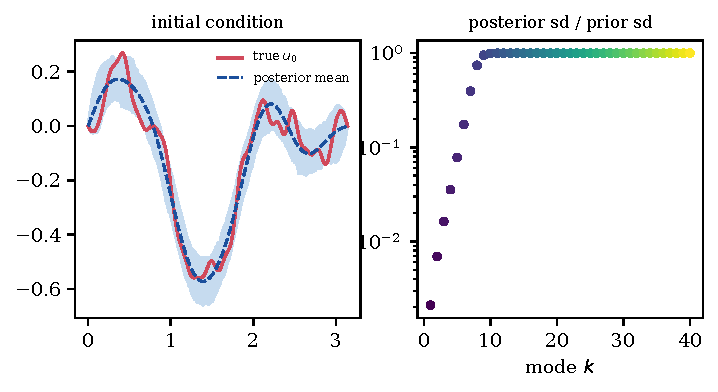
\includegraphics[width=\textwidth]{heat_inverse}
\caption{Inferring the initial condition of the heat equation from observations at time $T = 0.05$ with noise level $\delta = 0.002$, prior variances $\lambda_k = k^{-3}$ and $40$ Fourier modes. The truth is a draw from the prior. Left, truth, posterior mean and pointwise $90\%$ band computed from $200$ posterior draws; right, ratio of posterior to prior standard deviation by Fourier mode.}
\label{fig:heat_inverse}
\end{figure}

\begin{theorem}[Rates for the backward heat equation]
\label{thm:heat_rates}
Suppose $\lambda_k = k^{-1-2\alpha}$ with $\alpha>0$ and the true initial condition $\theta_0$ lies in a Sobolev ball of smoothness $\beta>0$. Then the posterior contracts in $L^2$ around the truth at the rate $(\log(1/\delta))^{-\min(\alpha,\beta)/2}$ up to constants, uniformly over the ball, and this is the minimax rate when $\alpha\geq\beta$. For a linear functional $L\theta = \sum_kl_k\theta_k$ whose coefficients satisfy $\sum_k|l_k|\,e^{2k^2T}k^{1+2\alpha}<\infty$ and $S = \sum_kl_k^2e^{2k^2T}>0$, let $\hat L = \sum_kl_ke^{k^2T}y_k$ be the unbiased estimator. Let $\Theta_B = \{\theta_0:\sup_k|\theta_{0,k}|\leq B\}$, a set that contains every Sobolev ball of smoothness $\beta\geq0$ and radius at most $B$, and let $\P_{\theta_0}$ be the law of the data under the truth $\theta_0$. Then for every $B>0$ and $\eta>0$, as $\delta\to0$,
\[
\sup_{\theta_0\in\Theta_B}\P_{\theta_0}\Big(\big\|\Pi\big((L\theta-\hat L)/\delta\in\cdot\mid y\big)-N(0,S)\big\|_{TV}>\eta\Big)\to0,
\]
and $(\hat L-L\theta_0)/\delta\sim N(0,S)$ exactly under the truth $\theta_0$. A Bernstein von Mises theorem therefore holds for $L\theta$, and equal tailed posterior credible intervals for $L\theta$ are asymptotically exact confidence intervals, uniformly over $\Theta_B$.
\end{theorem}

\begin{proof}
The $L^2$ rate is Theorem~2.1 of Knapik, van der Vaart and van Zanten~\cite{knapik2013}, with their prior scale equal to one and $n = \delta^{-2}$, and we do not repeat its proof. The mechanism is that modes $k\leq K_\delta$ are estimated with error of order $\delta e^{k^2T}$ while modes $k>K_\delta$ are left at the prior, and the tail $\sum_{k>K_\delta}(\theta_{0,k}^2+\lambda_k)$ is of order $K_\delta^{-2\min(\alpha,\beta)}$ with $K_\delta\asymp(\log(1/\delta))^{1/2}$.

For the functional, write $r_k = \delta^2e^{2k^2T}/(\lambda_k+\delta^2e^{2k^2T})\in[0,1]$, so that $v_k = \delta^2e^{2k^2T}(1-r_k)$ and the posterior mean of $\theta_k$ is $m_k = (1-r_k)e^{k^2T}y_k$. The posterior of $L\theta$ is Gaussian with mean $\sum_kl_km_k$ and variance $\sum_kl_k^2v_k = \delta^2\sum_kl_k^2e^{2k^2T}(1-r_k)$. Since $r_k\to0$ for each $k$ as $\delta\to0$ and $0\leq r_k\leq1$, dominated convergence gives $\sum_kl_k^2v_k = \delta^2(S+o(1))$, using $\sum_kl_k^2e^{2k^2T}\leq\sup_k|l_k|e^{k^2T}\sum_k|l_k|e^{k^2T}<\infty$. For the centering, substituting $y_k = e^{-k^2T}\theta_{0,k}+\delta\varepsilon_k$ under the truth,
\[
\sum_kl_km_k-\hat L = -\sum_kl_kr_k\theta_{0,k}-\delta\sum_kl_kr_ke^{k^2T}\varepsilon_k.
\]
The first term is bounded by $\sup_k|\theta_{0,k}|\sum_k|l_k|r_k\leq\delta^2B\sum_k|l_k|e^{2k^2T}\lambda_k^{-1} = O(\delta^2)$ uniformly over $\Theta_B$ by the summability assumption, since $\lambda_k^{-1} = k^{1+2\alpha}$. The second term is centered Gaussian with variance $\delta^2\sum_kl_k^2r_k^2e^{2k^2T} = o(\delta^2)$ by dominated convergence, a variance that does not depend on $\theta_0$. Hence $(\sum_kl_km_k-\hat L)/\delta\to0$ in $\P_{\theta_0}$ probability, uniformly over $\Theta_B$, and the posterior of $(L\theta-\hat L)/\delta$ is a Gaussian whose mean tends to zero and whose variance tends to $S>0$; convergence of Gaussian laws in total variation follows from convergence of their parameters. Under the truth, $\hat L-L\theta_0 = \delta\sum_kl_ke^{k^2T}\varepsilon_k\sim N(0,\delta^2S)$ exactly. An equal tailed credible interval for $L\theta$ therefore has endpoints $\hat L\pm z\delta\sqrt S+o(\delta)$ in probability, uniformly over $\Theta_B$, where $z$ is a normal quantile, and its coverage tends to the nominal level.
\end{proof}

The first part of the theorem is due to Knapik, van der Vaart and van Zanten~\cite{knapik2013}, who also show that credible balls for the whole initial condition have asymptotic coverage zero when the prior is smoother than the truth and coverage one, with a radius larger than that of a confidence ball by a diverging factor, when it is rougher. For linear functionals whose coefficients decay only polynomially they show that credible intervals have asymptotic coverage zero or one, so that no Bernstein von Mises theorem holds for them. The second part of the theorem is proved above. For the direct white noise model, Bernstein von Mises theorems for linear and nonlinear functionals are due to Castillo and Nickl~\cite{castillonickl2013}. The reconstruction of the whole initial condition is possible only at logarithmic rates; no method can do better uniformly over a Sobolev ball. But smooth functionals of the initial condition, those whose coefficients decay faster than the damping, are estimable at the parametric rate, and the Bayesian posterior quantifies their uncertainty correctly. Inference on the solution manifold is therefore an exercise in choosing the questions the data can answer.

\section{The nonlinear theory}

For nonlinear forward maps the corresponding theory was developed by Nickl and coauthors and is presented in Nickl's lectures~\cite{nickl2023book}. Its architecture has three components.

The first is a \emph{forward regularity} estimate: the map $\mathcal{G}:\theta\mapsto(\mathcal{O}_j\Phi_{t_j}\theta)_j$ is Lipschitz, with polynomial growth of the constant, from the parameter space to the observation space. For Navier Stokes in two dimensions this follows from energy estimates.

The second is a \emph{stability} estimate in the reverse direction: $\|\theta-\theta'\|_{H^{-s}}\leq\chi(\|\mathcal{G}(\theta)-\mathcal{G}(\theta')\|)$ for some modulus $\chi$, valid on bounded sets of a smoother space. For parabolic problems observed only at positive times $\chi$ is typically logarithmic, as in the linear case. Combined with posterior contraction in the observation space, which holds at the usual rates by general theory for Gaussian priors rescaled with the sample size, stability transfers contraction to the parameter.

The third is \emph{computation}. Nickl and Wang~\cite{nicklwang2024} showed, for one model, that a lower bound on the Fisher information operator called gradient stability makes the log likelihood strongly concave near the truth, and that a Langevin type algorithm, initialized by a suitable estimator and run on a surrogate of the posterior, then samples from it to given accuracy in a number of steps polynomial in the dimension and the sample size (Section~\ref{sec:gradstab}).

For time evolution equations, Nickl and Titi~\cite{nickltiti2024} proved posterior consistency for the two dimensional Navier Stokes equations, with inverse logarithmic rates for the initial condition, and showed that in general no faster rate is possible when the observation times are sampled from a window bounded away from zero. When the observations are spread over space and time starting at time zero, the stability estimate improves and the posterior contracts at a polynomial rate in the number $N$ of observations~\cite{konennickl2026}. For such observations Nickl proved a Bernstein von Mises theorem for reaction diffusion equations~\cite{nicklbvm2024}, and Konen and Nickl proved one for Navier Stokes~\cite{konennickl2026}: the posterior law of the trajectory, centered at the posterior mean and scaled by $\sqrt N$, is close to a Gaussian law in Wasserstein distance for the supremum norm over any time window bounded away from zero. Our own work~\cite{polsonsokolov2026manifold} combines this theory with simulation based computation, as we now describe and as Chapters~\ref{ch:manifold} to~\ref{ch:examples} treat in detail.

\section{Gradient stability and polynomial time sampling}
\label{sec:gradstab}

\subsubsection{The computational question} The posterior of a nonlinear partial differential equation inverse problem is a density on $\R^D$ with $D$ large, and it is not log concave, because the forward map is nonlinear and enters the log likelihood through a square. A Markov chain can take a time exponential in $D$ to mix, and since the posterior becomes spiked as $N$ grows, iterative algorithms can take a time exponential in $N$ to leave a neighborhood of a local optimum~\cite{nicklwang2024}. The preconditioned Crank Nicolson chain of Section~\ref{sec:dimrobust} has a spectral gap independent of the discretization~\cite{hairer2014}, but the bound is not quantitative in $N$ and $D$~\cite{nicklwang2024}. The question is when the posterior mean can be computed to accuracy $\varepsilon$ in a number of steps polynomial in $N$, $D$ and $\varepsilon^{-1}$, with high probability under the data. Nickl and Wang answer it for one model, under a hypothesis on the forward map called gradient stability. We ask where it holds, above all for the two dimensional Navier Stokes equations. Numbers of theorems, lemmas and equations of Nickl and Wang, of Konen and Nickl and of Castre and Nickl refer to the arXiv versions 2009.05298v2, 2507.18279v2 and 2601.10326v1.

\subsubsection{Setting} We use the notation of Nickl and Wang, with the forward map written $\mathcal{G}$, $P^X$ the uniform probability measure on a bounded set $\mathcal{X}$ and $\|\cdot\|_{L^2}$ the norm of $L^2(P^X)$. For $\theta\in\R^D$, the coefficients of the unknown in the first $D$ basis elements, the data $Z_i=(Y_i,X_i)$ satisfy
\begin{equation}\label{eq:gs_model}
Y_i=\mathcal{G}(\theta)(X_i)+\varepsilon_i,\qquad X_i\sim P^X,\quad\varepsilon_i\sim N(0,1),\qquad i=1,\dots,N,
\end{equation}
all independent, under a truth $\theta_0$ that need not lie in $\R^D$ (we write $\P_{\theta_0}^N$ and $\E_{\theta_0}$). For an evolution equation, $\mathcal{X}=[0,T]\times\T^d$ and $\mathcal{G}(\theta)(t,x)$ is the solution at time $t$ and position $x$. This is the observation model~\eqref{eq:observation_model} with $\mathcal{O}_j$ the evaluation at a random point of space and time and unit noise. With $\ell(\theta,Z)=-\frac12(Y-\mathcal{G}(\theta)(X))^2$, $\ell_N(\theta)=\sum_{i\le N}\ell(\theta,Z_i)$ and a Gaussian prior $N(0,\Sigma)$ with density $\pi$, the posterior $\Pi(\cdot\mid Z)$ has density proportional to $e^{\ell_N}\pi=e^{-H}$, where $H(\theta)=-\ell_N(\theta)+\frac12\theta^\top\Sigma^{-1}\theta$.

\subsubsection{Gradient stability} Differentiating $\ell$ twice and using $\E_{\theta_0}[Y\mid X]=\mathcal{G}(\theta_0)(X)$ gives, for every $v\in\R^D$,
\begin{equation}\label{eq:gs_hess}
\begin{aligned}
v^\top\E_{\theta_0}\big[-\nabla^2\ell(\theta,Z)\big]v={}&\big\|v^\top\nabla\mathcal{G}(\theta)\big\|_{L^2}^2\\
&+\big\langle\mathcal{G}(\theta)-\mathcal{G}(\theta_0),\,v^\top\nabla^2\mathcal{G}(\theta)v\big\rangle_{L^2}.
\end{aligned}
\end{equation}
At $\theta=\theta_0$, when this lies in $\R^D$, the second term vanishes and the matrix is the Fisher information $I(\theta_0)=\E_X[\nabla\mathcal{G}(\theta_0)(X)\nabla\mathcal{G}(\theta_0)(X)^\top]$ of one observation. The expected Hessian of $-\ell_N$ is $N$ times this matrix, so a lower bound on its smallest eigenvalue says that the data are informative in every direction, and by~\eqref{eq:gs_hess} it follows from an injectivity estimate for the gradient.

\begin{definition}[Gradient stability]\label{def:gs_stab}
Let $B\subset\R^D$ and $c>0$. The forward map $\mathcal{G}$ is gradient stable on $B$ with constant $c$ if $\theta\mapsto\mathcal{G}(\theta)(x)$ is differentiable on $B$ for every $x$ and
\begin{equation}\label{eq:gs_stab}
\big\|v^\top\nabla\mathcal{G}(\theta)\big\|_{L^2}\ge c\,|v|\qquad\text{for all }\theta\in B\text{ and }v\in\R^D.
\end{equation}
\end{definition}

Nickl and Wang take $B=\{\theta:|\theta-\theta^*|_1<\eta\}$, with $\theta^*\in\R^D$ a centering point (the projection of $\theta_0$) and $|\theta|_1^2=\theta^\top M\theta$ for a symmetric positive definite matrix $M$. The difficulty lies in the dependence of the constant $c$ on $D$, which Castre and Nickl~\cite{castrenickl2026} make explicit. What enters the theorem is the local curvature condition
\begin{equation}\label{eq:gs_curv}
\inf_{\theta\in B}\lambda_{\min}\big(\E_{\theta_0}[-\nabla^2\ell(\theta,Z)]\big)\ge c_{\min}>0 .
\end{equation}
It follows from~\eqref{eq:gs_stab} by a line that we add. If $k_0$ and $k_2$ bound the supremum norms of $\mathcal{G}(\theta)-\mathcal{G}(\theta_0)$ and of $\|\nabla^2\mathcal{G}(\theta)\|_{\mathrm{op}}$ over $B$, the second term of~\eqref{eq:gs_hess} is at least $-k_0k_2|v|^2$ by the Cauchy Schwarz inequality, so gradient stability with constant $c$ and $k_0k_2\le c^2/2$ give~\eqref{eq:gs_curv} with $c_{\min}=c^2/2$.

The Bernstein von Mises theory of this chapter rests on invertibility of the information operator, the derivative of the forward map composed with its adjoint, between Sobolev spaces, which Konen and Nickl~\cite{konennickl2026} prove for the two dimensional Navier Stokes equations. Gradient stability is its quantitative counterpart on $D$ coordinates. It is local, and hence weaker than the Polyak \L{}ojasiewicz condition of nonconvex optimization, a global lower bound on the squared gradient by the suboptimality, as Nickl and Wang remark.

\subsubsection{The theorem of Nickl and Wang} \emph{Local regularity} asks that $\mathcal{G}(\theta)(x)$ be twice continuously differentiable in $\theta\in B$, with $\mathcal{G}(\theta)-\mathcal{G}(\theta_0)$, $\nabla\mathcal{G}(\theta)$ and $\nabla^2\mathcal{G}(\theta)$ bounded in the supremum norm over $x$ by $k_0,k_1,k_2$ and Lipschitz in $\theta$ for $|\cdot|_1$ with constants $m_0,m_1,m_2$. \emph{Local curvature} asks for~\eqref{eq:gs_curv} and for a bound $c_{\max}\ge c_{\min}$ on the expected log likelihood and its first two derivatives over $B$. The algorithm needs an initializer $\theta_{\mathrm{init}}\in\R^D$ computed from the data and a surrogate $\tilde\ell_N=\alpha_\eta\ell_N-Kg_\eta$ of the log likelihood. Here $\alpha_\eta$ is a smooth cutoff in $|\theta-\theta_{\mathrm{init}}|_1/\eta$, $g_\eta$ is a convex penalty that vanishes for $|\theta-\theta_{\mathrm{init}}|_1\le\eta/2$, and $K>0$ is large. The surrogate posterior $\tilde\Pi(\cdot\mid Z)$ has density proportional to $e^{\tilde\ell_N}\pi$, and the unadjusted Langevin algorithm (ULA) for it, with step size $\gamma>0$ and independent $\xi_k\sim N(0,I_D)$, is
\begin{equation}\label{eq:gs_ula}
\vartheta_0=\theta_{\mathrm{init}},\qquad\vartheta_{k+1}=\vartheta_k+\gamma\big(\nabla\tilde\ell_N(\vartheta_k)-\Sigma^{-1}\vartheta_k\big)+\sqrt{2\gamma}\,\xi_{k+1}.
\end{equation}
Three events enter. On $E_{\mathrm{conv}}$, $\lambda_{\min}(-\nabla^2\ell_N(\theta))\ge Nc_{\min}/2$ and $|\ell_N|+|\nabla\ell_N|+\|\nabla^2\ell_N\|_{\mathrm{op}}\le N(5c_{\max}+1)$ for all $\theta\in B$. Further $E_{\mathrm{init}}=\{|\theta_{\mathrm{init}}-\theta^*|_1\le\eta/8\}$ and $E_{\mathrm{wass}}(\rho)=\{W_2^2(\Pi(\cdot\mid Z),\tilde\Pi(\cdot\mid Z))\le\rho/2\}$, where $W_2$ is the Wasserstein distance of Chapter~\ref{ch:entropy}.

\begin{theorem}[Nickl and Wang, in simplified form]\label{thm:gs_main}
Let the data follow~\eqref{eq:gs_model}, let the prior be $N(0,\Sigma)$ and let local regularity and local curvature hold on $B$ with $\eta\in(0,1]$. Let $R_N$ be the quantity of equation~(45) of~\cite{nicklwang2024}, a universal constant times $N$ times the minimum of eight ratios of the constants above; in particular $R_N\le CNc_{\min}^2/(k_1^2+k_0k_2+k_2)^2$.
\begin{enumerate}[label=(\roman*),nosep]
\item If $D\le R_N$, then $\P_{\theta_0}^N(E_{\mathrm{conv}})\ge1-32e^{-R_N}-e^{-N/8}$.
\item Let $D\le R_N$, $K\ge CN(c_{\max}+1)(1+\lambda_{\max}(M)\eta^{-2})/\lambda_{\min}(M)$, $m=\frac12Nc_{\min}+\lambda_{\min}(\Sigma^{-1})$ and $\Lambda=7K\lambda_{\max}(M)+\lambda_{\max}(\Sigma^{-1})$. Then for every $\rho>0$, $0<\gamma\le1/(m+\Lambda)$ and $k\ge0$, on $E=E_{\mathrm{conv}}\cap E_{\mathrm{init}}\cap E_{\mathrm{wass}}(\rho)$,
\begin{equation}\label{eq:gs_w2}
W_2^2\big(\Law(\vartheta_k),\Pi(\cdot\mid Z)\big)\le\rho+b(\gamma)+4\Big(\tau+\frac Dm\Big)\Big(1-\frac{\gamma m}2\Big)^k,
\end{equation}
where $b(\gamma)=c_1(\gamma D\Lambda^2m^{-2}+\gamma^2D\Lambda^4m^{-3})$, $\tau=c_2\kappa(\Sigma)(1+\eta^2/\lambda_{\min}(M)+R^2)$ for any $R\ge|\theta^*|$, $\kappa(\Sigma)=\lambda_{\max}(\Sigma)/\lambda_{\min}(\Sigma)$, and $C,c_1,c_2$ are universal constants.
\end{enumerate}
\end{theorem}

Part (i) is Lemma~3.4 and part (ii) is Proposition~3.6 with Theorem~3.7 of~\cite{nicklwang2024}. Their Theorem~3.7 allows $0<\gamma\le1/\Lambda$; its proof applies, through their Proposition~A.4, Theorem~5 of Durmus and Moulines~\cite{durmusmoulines2019}, which is proved for $\gamma\le1/(m+\Lambda)$, and we state (ii) in that range. Since $m\le\Lambda$, this costs at most a factor $2$ in the step, and for large $N$ the range contains the step sizes used below. We quote the theorem without proof. The theorem does not say that $E_{\mathrm{init}}$ and $E_{\mathrm{wass}}(\rho)$ have high probability. Bounding their probability, Nickl and Wang write, `may pose a formidable challenge in its own right', and they do it for the Schr\"odinger equation only.

\begin{corollary}[Posterior mean and mode]\label{cor:gs_mean}
In the setting of Theorem~\ref{thm:gs_main}(ii) let $\bar\vartheta$ be the average of $\vartheta_{J_{\mathrm{in}}+1},\dots,\vartheta_{J_{\mathrm{in}}+J}$.
\begin{enumerate}[label=(\alph*),nosep]
\item There are constants $c_3,c_5>0$ such that on $E$, for $t\ge\sqrt8\,(\rho+b(\gamma))^{1/2}$, $mJ\gamma\ge1$ and $J_{\mathrm{in}}\ge(c_3/m\gamma)\log\big(1+(\rho+b(\gamma))^{-1}+\tau+D/m\big)$, $\P_{\theta_{\mathrm{init}}}(|\bar\vartheta-\E^\Pi[\theta\mid Z]|\ge t)\le2D\exp(-c_5t^2m^2J\gamma/D)$.
\item If the posterior density has a maximizer and every maximizer lies in $\{|\theta-\theta^*|_1\le3\eta/8\}$, then on $E_{\mathrm{conv}}\cap E_{\mathrm{init}}$ the posterior has a unique mode, and gradient ascent on the logarithm of the surrogate density from $\theta_{\mathrm{init}}$ with step $(2\Lambda)^{-1}$ converges to it, with squared error at most a constant, which depends on the data, times $(1-m/(2\Lambda))^k$.
\end{enumerate}
\end{corollary}

Part (a) is Corollary~3.9 of~\cite{nicklwang2024}, quoted without proof, with the factor $1+1/(mJ\gamma)\le2$ in the exponent of their bound absorbed in $c_5$. Part (b) is our formulation of their Proposition~A.2 and of the argument after their equation~(158), and the argument is short. On $E_{\mathrm{conv}}\cap E_{\mathrm{init}}$ the surrogate $\tilde\ell_N$ and $\ell_N$ have the same gradient on the ball of (b), so a maximizer of the posterior density is a critical point of the logarithm of the surrogate density, which is strongly concave and has one critical point only. Proposition~A.2 is the geometric rate of gradient descent for a function whose Hessian lies between $mI$ and $\Lambda I$. With $\rho\le\varepsilon^2/16$ and $b(\gamma)\le\varepsilon^2/16$ the threshold for $t$ is at most $\varepsilon$, and the number of steps is polynomial in $N$, $D$, $m^{-1}$, $\Lambda$ and $\varepsilon^{-1}$.

\subsubsection{The Schr\"odinger equation} Nickl and Wang prove $E_{\mathrm{init}}$ and $E_{\mathrm{wass}}$ for the steady state Schr\"odinger equation $\frac12\Delta u-fu=0$ on a bounded smooth domain $\mathcal{O}\subset\R^d$, $d\le3$, of unit volume, with boundary values $u=g$, an elliptic boundary value problem. The unknown is $f_\theta=\Phi\circ F_\theta$, where $F_\theta=\sum_{k\le D}\theta_ke_k$ in the eigenfunctions of the Dirichlet Laplacian, with eigenvalues $\lambda_k$, and $\Phi$ is a regular link function. The forward map is $\mathcal{G}(\theta)=u_{f_\theta}$, the design is uniform on $\mathcal{O}$, and the prior is $N(0,N^{-d/(2\alpha+d)}\Lambda_\alpha^{-1})$ with $\Lambda_\alpha=\diag(\lambda_1^\alpha,\dots,\lambda_D^\alpha)$ and an integer $\alpha>6$.

\begin{theorem}[Nickl and Wang, Schr\"odinger equation, in simplified form]\label{thm:gs_schr}
Let $\theta_0$ satisfy $\sum_k\lambda_k^\alpha\theta_{0,k}^2<\infty$, and for some constants $c_0>0$ and $0<c_0'<1/2$ let $D\le c_0N^{d/(2\alpha+d)}$ and $\|\mathcal{G}(\theta_{0,D})-\mathcal{G}(\theta_0)\|_{L^2}\le c_0'N^{-\alpha/(2\alpha+d)}$, where $\theta_{0,D}$ is the projection of $\theta_0$ onto $\R^D$. Run~\eqref{eq:gs_ula} with $M=I$, $\theta^*=\theta_{0,D}$, $\eta=D^{-4/d}/\log N$, $K=ND^{8/d}(\log N)^3$, $\gamma\le(ND^{8/d}(\log N)^4)^{-1}$ and the initializer of Theorem~B.6 of~\cite{nicklwang2024}. On events of probability at least $1-ce^{-c'N^{d/(2\alpha+d)}}$, for every $P>0$ and $\varepsilon\ge N^{-P}$:
\begin{enumerate}[label=(\roman*),nosep]
\item there are a step size and a number of steps $O(N^{b_1}D^{b_2}\varepsilon^{-b_3})$ after which $W_2(\Law(\vartheta_k),\Pi(\cdot\mid Z))\le\varepsilon$, and averaging the chain computes the posterior mean to accuracy $\varepsilon$ at a cost of the same form; the exponents $b_1,b_2,b_3>0$ are not specified and may differ between the two statements;
\item the posterior has a unique mode, and gradient ascent on the logarithm of the surrogate density with step size $(ND^{8/d}(\log N)^4)^{-1}$ comes within $cN^{-\alpha^2/((2\alpha+d)(\alpha+2))}$ of $\theta_0$ in $\ell^2$ after $O(D^{12/d}(\log N)^5)$ iterations.
\end{enumerate}
\end{theorem}

We quote the theorem without proof. It collects Theorem~1.1 and Theorems~2.5, 2.7 and~2.8 of~\cite{nicklwang2024}, which are Theorem~\ref{thm:gs_main} and Corollary~\ref{cor:gs_mean} with the scalings of their Proposition~4.1, together with their Theorems~B.6 and~4.14 for $E_{\mathrm{init}}$ and $E_{\mathrm{wass}}$. The scalings are $k_0\simeq k_1\simeq1$, $k_2\simeq m_0\simeq m_1\simeq D^{2/d}$, $m_2\simeq D^{4/d}$, $c_{\max}\simeq1$ and, from an elliptic stability estimate, $c_{\min}\simeq D^{-4/d}$. Then $R_N\simeq ND^{-12/d}$, $m\simeq ND^{-4/d}$, $\Lambda\simeq ND^{8/d}(\log N)^3$ and $\Lambda/m\simeq D^{12/d}(\log N)^3$. Reading~\eqref{eq:gs_w2} with these values, accuracy $\tilde\varepsilon=\varepsilon m^{1/2}$ in units of the posterior scale takes about $D^{1+24/d}(\log N)^6\tilde\varepsilon^{-2}$ steps, of degree thirteen in $D$ for $d=2$.

\begin{remark}[Scope of the example]\label{rem:gs_scope}
The equation is elliptic and steady: there is no time, the unknown is a coefficient, and the design fills the domain. The guarantee is local and needs a warm start in a ball of radius of order $D^{-4/d}/\log N$ around $\theta_{0,D}$, which the initializer reaches by estimating $u$ by convex penalized least squares and inverting the equation, $f=\Delta\hat u/(2\hat u)$, at the price of two derivatives. A cold start can fail even for a unimodal target~\cite{bandeira2023}. Theorem~\ref{thm:gs_main} is therefore a template and not a theorem about every gradient stable forward map.
\end{remark}

\begin{proof}[Sketch of the proof of Theorem~\ref{thm:gs_main}]
\emph{(a) Local strong convexity of $-\ell_N$.} By Weyl's inequality it suffices to keep the empirical Hessian within $Nc_{\min}/2$ of its mean uniformly on $B$. A net of the unit sphere of mesh $1/4$, with at most $9^D$ points, reduces the operator norm to a maximum over the net, up to a factor two. For a fixed direction the centered quadratic form splits into its value at $\theta^*$, handled by Hoeffding's and Bernstein's inequalities, and an increment over $\theta\in B$, an empirical process that generic chaining controls (Lemma~3.12 of~\cite{nicklwang2024}). The probability bounds beat the union bound $9^D$ when $D\le R_N$. This is part~(i).

\emph{(b) A strongly log concave surrogate.} On $E_{\mathrm{conv}}\cap E_{\mathrm{init}}$, $\tilde\ell_N=\ell_N$ on $\{|\theta-\theta^*|_1\le3\eta/8\}$, $-\nabla^2\tilde\ell_N\succeq\frac12Nc_{\min}I$ on all of $\R^D$ and $\nabla\tilde\ell_N$ is $7K\lambda_{\max}(M)$ Lipschitz (Proposition~3.6 of~\cite{nicklwang2024}). Within distance $3\eta/4$ of $\theta_{\mathrm{init}}$ the cutoff equals one and the penalty is convex, so $-\nabla^2\tilde\ell_N$ inherits the curvature that $E_{\mathrm{conv}}$ gives. Beyond it, on $E_{\mathrm{conv}}$ the Hessian of $\alpha_\eta\ell_N$ is at most of order $N(c_{\max}+1)(1+\lambda_{\max}(M)\eta^{-2})$ in norm, while the Hessian of $Kg_\eta$ is at least $K\lambda_{\min}(M)/3$, so the condition on $K$ lets the penalty dominate. With the prior, $\tilde U=-\tilde\ell_N+\frac12\theta^\top\Sigma^{-1}\theta$ satisfies $mI\preceq\nabla^2\tilde U\preceq\Lambda I$.

\emph{(c) Langevin sampling of a strongly log concave target.} Let $\mu\propto e^{-U}$ with $mI\preceq\nabla^2U\preceq\Lambda I$. The law of the Langevin diffusion $\dd L_t=-\nabla U(L_t)\dd t+\sqrt2\,\dd W_t$ solves the Fokker Planck equation~\eqref{eq:fp} with $V=U$, and by Theorem~\ref{thm:jko} it is the Wasserstein gradient flow of $\KL(\cdot\,\|\,\mu)$. The criterion of Bakry and \'Emery~\cite{bakry1985}, stated after Theorem~\ref{thm:lsi}, turns $\nabla^2U\succeq mI$ into a log Sobolev inequality with constant $2/m$, hence $\KL(\rho_t\|\mu)\le e^{-2mt}\KL(\rho_0\|\mu)$, and Talagrand's inequality $W_2^2\le(2/m)\KL$ transfers the decay to $W_2$. The discrete time bound that~\eqref{eq:gs_ula} needs is due to Durmus and Moulines~\cite{durmusmoulines2019}, after~\cite{dalalyan2017,durmusmoulines2017}. The chain starts at a point, whose relative entropy is infinite, so the bound is in $W_2$: for $0<\gamma\le1/(m+\Lambda)$ and $\theta_U$ the minimizer of $U$ (Theorem~5 of~\cite{durmusmoulines2019}, in the form of Proposition~A.4 of~\cite{nicklwang2024}),
\[
\begin{aligned}
W_2^2(\Law(\vartheta_k),\mu)\le{}&2\Big(1-\frac{m\gamma}2\Big)^k\Big(|\theta_{\mathrm{init}}-\theta_U|^2+\frac Dm\Big)\\
&+\frac{18\gamma D\Lambda^2}{m^2}+\frac{6\gamma^2D\Lambda^4}{m^3}.
\end{aligned}
\]
The first term decays geometrically in $k$, as $e^{-2mt}$ does in $t$ for the diffusion, but at the weaker rate $m\gamma/2$ per step instead of $2m\gamma$. The others, which have no counterpart in Chapter~\ref{ch:entropy}, are the bias of the Euler scheme. With $\gamma\simeq\varepsilon^2m^2/(D\Lambda^2)$ the bias is of order $\varepsilon^2$, and $k\simeq(\Lambda/m)^2D(\varepsilon^2m)^{-1}\log(\cdot)$ steps suffice.

\emph{(d) From the surrogate to the posterior.} The penalty puts the maximizer of $\tilde\ell_N$ within a distance of order $1+\eta\lambda_{\min}(M)^{-1/2}$ of $\theta_{\mathrm{init}}$, and the prior moves the mode of $\tilde\Pi$ by an amount controlled by $\kappa(\Sigma)$, so $|\theta_{\mathrm{init}}-\theta_U|^2\lesssim\tau$ for $\mu=\tilde\Pi$. The triangle inequality for $W_2$ and $W_2^2(\Pi,\tilde\Pi)\le\rho/2$ then give~\eqref{eq:gs_w2}. For the Schr\"odinger equation Theorem~4.14 of~\cite{nicklwang2024} bounds $E_{\mathrm{wass}}$: $W_2^2$ is at most twice the integral of $|\theta-\theta_1|^2$ against $|\Pi-\tilde\Pi|$ for every point $\theta_1$ (Theorem~6.15 of~\cite{villani2009}), and for $\theta_1$ the posterior mode the two measures agree up to normalizing constants near $\theta_1$ and carry exponentially small mass away from it.
\end{proof}

\subsubsection{Where the log Sobolev inequality enters} The proof uses the theory of Chapter~\ref{ch:entropy} in step (c) and only there, and for the surrogate and not for the posterior, which is not strongly log concave and for which Nickl and Wang prove no log Sobolev inequality. Results that assume a log Sobolev or Poincar\'e inequality for the target~\cite{chewi2025}, or that it is convex outside a ball~\cite{ma2019}, yield bounds exponential in $N$ when applied to the posterior without further work, as Nickl and Wang observe: the Holley Stroock principle~\cite{holleystroock1987} costs a factor exponential in the oscillation of $\ell_N$, which is of order $N$ for a bounded forward map, and the bound of Ma and coauthors is exponential in the Lipschitz constant of $\nabla\ell_N$. The theorem rests on strong log concavity of the surrogate, its closeness to the posterior and the initializer.

\subsubsection{Where gradient stability is known} Nickl and Wang verify gradient stability for the steady state Schr\"odinger equation (their Lemma~4.7), and Bohr and Nickl~\cite{bohrnickl2024} extend the theory and verify its stability conditions for the non Abelian X ray transform. Castre and Nickl~\cite{castrenickl2026} list further parameter identification problems with linear equations where gradients of forward maps have been computed, among them Darcy's problem~\cite{nickl2023book,altmeyer2022}, and initial value to solution maps of reaction diffusion and Navier Stokes equations, see the next subsection. They write that these proofs do not extend straightforwardly to a general parameter of a nonlinear equation, where two nonlinearities meet. Their device is the implicit function theorem: $f(\theta,\mathcal{G}(\theta))=0$ gives $D\mathcal{G}=-(D_2f)^{-1}D_1f$, and gradient stability reduces to injectivity of $D_1f$. For a reaction diffusion equation with unknown reaction term they prove differentiability of the parameter to solution map (their Theorem~2.1) and only sketch gradient stability (Remark~2.2).

\begin{remark}[Castre and Nickl: the McKean Vlasov equation]\label{rem:gs_cn}
Let $\rho_W$ solve $\partial_t\rho=\Delta\rho+\nabla\cdot(\rho\nabla W*\rho)$ on $[0,T]\times\T^d$ with a smooth initial condition $\varphi$ bounded below and an unknown interaction potential $W$ of degree at most $K$ in the trigonometric basis, so $D\simeq K^d$, and let $\rho_W$ be observed as in~\eqref{eq:gs_model}. Assume that $|\hat\varphi_k|\ge c_*|k|^{-\zeta}$ for a large enough $\zeta$, which excludes the steady state $\varphi=1$~\cite{nickl2025}. Gradient stability holds with constant of order $K^{-3\zeta}$ (their Theorem~2.14), and $c_{\min}\ge c_0D^{-6\zeta/d}$ on a ball around the truth of radius polynomially small in $D$ (Theorem~3.3). The posterior is $W_2$ close to a log concave surrogate with probability tending to one (Theorem~3.10), and \emph{if a feasible initializer exists} ULA mixes in a time polynomial in $\varepsilon^{-1}$, $D$ and $N$ (Theorem~3.11). The initializer is assumed, not constructed, and the unknown is a parameter and not an initial condition.
\end{remark}

\subsubsection{The initial condition problem} For the initial condition of the two dimensional Navier Stokes equations, Nickl and Titi~\cite{nickltiti2024} prove posterior consistency at inverse logarithmic rates, and show that no faster rate is possible when the observation times lie in $[T_0,T]$ with $T_0>0$. For initial conditions on the global attractor of a two dimensional periodic reaction diffusion system, Konen and Nickl~\cite{konennickl2026attractor} show that the initial condition and the states can be recovered from discrete measurements at near parametric rates. For times sampled from $[0,T]$, Nickl~\cite{nicklbvm2024} proves a Bernstein von Mises theorem for the trajectory of dissipative systems such as reaction diffusion, and Konen and Nickl~\cite{konennickl2026} prove one for Navier Stokes, with polynomial contraction rates for the initial condition (their Theorem~2.2) and invertibility of the information operator (Theorem~2.6). None of this is a theorem about computation. Konen and Nickl say only that provably reliable computation `can be expected to be possible in polynomial time in relevant parameters' by an MCMC algorithm combining the ideas of Nickl and Wang with their estimates, started at the boundary trace of a smoothing estimator, and that the details will be studied elsewhere. We have not found a later paper that turns these expectations into theorems.

What the estimates of Konen and Nickl do give is the first ingredient. The velocity is vector valued, and Remark~3.11 of~\cite{nicklwang2024} extends the theory to values in a finite dimensional inner product space, with the norm of that space in the likelihood and in $\|\cdot\|_{L^2}$. The following statement is our deduction from their Propositions~3.10 and~3.12, and not a result of their paper.

\begin{proposition}[Gradient stability for the initial condition of two dimensional Navier Stokes, with time zero observed]\label{prop:gs_ns}
Let $\nu,T,L>0$ and $f\in\Hds1$, let $\mathcal{X}=[0,T]\times\T^2$ with the uniform probability measure, let $e_1,e_2,\dots$ be the eigenfunctions of the Stokes operator on $\T^2$ with eigenvalues $\lambda_1\le\lambda_2\le\cdots$, and let $\mathcal{G}(\theta)(t,x)=u_\theta(t,x)$ be the velocity of the Navier Stokes solution with viscosity $\nu$, forcing $f$ and initial condition $\sum_{k\le D}\theta_ke_k$. There is $c>0$, depending only on $\nu$, $T$, $\|f\|_{\Hds1}$, $L$ and the torus, such that $\|v^\top\nabla\mathcal{G}(\theta)\|_{L^2(\mathcal{X})}\ge c\,D^{-1/2}|v|$ for every $D$, every $v\in\R^D$ and every $\theta\in\R^D$ with $\|\sum_k\theta_ke_k\|_{\Hds2}\le L$.
\end{proposition}

\begin{proof}
By Proposition~3.12 of Konen and Nickl, $\theta\mapsto u_\theta$ is differentiable with derivative the linearization $\I_\theta$ of the flow, so $v^\top\nabla\mathcal{G}(\theta)(t,\cdot)=\I_\theta[\xi_v](t)$ for $\xi_v=\sum_{k\le D}v_ke_k$. Their Proposition~3.10, with $a=-1$ and $a^*=2$, gives $\|\xi\|_{\Hds{-1}}^2\le C\int_0^T\|\I_\theta[\xi](t)\|_{L^2}^2\dd t$ for $\|\theta\|_{\Hds2}\le L$, with $C$ depending on $\nu,T,\|f\|_{\Hds1},L$. Hence, with the uniform probability measure on $\mathcal{X}$, $\|v^\top\nabla\mathcal{G}(\theta)\|_{L^2(\mathcal{X})}^2=(T|\T^2|)^{-1}\int_0^T\|\I_\theta[\xi_v](t)\|_{L^2}^2\dd t\ge(CT|\T^2|)^{-1}\|\xi_v\|_{\Hds{-1}}^2=(CT|\T^2|)^{-1}\sum_kv_k^2/\lambda_k\ge(CT|\T^2|)^{-1}|v|^2/\lambda_D$, and $\lambda_D\asymp D$ by Weyl's law in two dimensions.
\end{proof}

The constant is polynomial in $D$, which is what a design that includes time zero buys, but it is only the first ingredient. Curvature on a ball needs $k_0k_2\le c^2/(2D)$ there, and local regularity needs derivatives of the flow up to order three in the first $D$ coordinates, with bounds polynomial in $D$. Konen and Nickl bound the flow and its first derivative in Sobolev norms (their Propositions~3.7 and~3.9), which with the Sobolev embedding of $\Hds2$ into the continuous functions gives $k_0$, $k_1$ and $m_0$ polynomial in $D$ for $\theta$ in a ball of $\Hds2$, because $\|\sum_{k\le D}v_ke_k\|_{\Hds2}\lesssim\lambda_D|v|$, and they bound the quadratic Taylor remainder (their Proposition~3.12). We have not found bounds for the second and third derivatives of the flow, which $k_2$, $m_1$ and $m_2$ need. The warm start needs an initializer within the radius $\eta/8$ of the projection of the truth, and the boundary trace of a smoothing estimator is a candidate whose accuracy at time zero has to be proved. The event $E_{\mathrm{wass}}$ needs exponentially small posterior mass outside the ball, whereas the contraction theorem of Konen and Nickl holds in probability. Whether these steps can be taken is open as far as we know.

\subsubsection{A computation for the heat equation} Observation that begins after time zero changes the constant. Take $\mathcal{G}(\theta)(t,\cdot)=\sum_{k\le D}e^{-k^2t}\theta_k\phi_k$, the heat equation of Section~\ref{sec:linearheat} with the basis orthonormal in $L^2(P^X)$. It is linear, so $\nabla^2\mathcal{G}=0$ and by~\eqref{eq:gs_hess} the expected Hessian of $-\ell_N$ is $N\diag(\iota_1,\dots,\iota_D)$ at every $\theta$, where $\iota_k=\E[e^{-2k^2t}]$ is the information that one observation carries about mode $k$. Gradient stability holds on all of $\R^D$ with $c^2=c_{\min}=\min_{k\le D}\iota_k$. At a single time $T$, $\iota_k=e^{-2k^2T}$. For times uniform on $[T_0,T]$ it is the quantity of~\eqref{m:eq:iota} with $\nu\lambda_j=k^2$, of order $(2k^2T)^{-1}$ if $T_0=0$ and of order $e^{-2k^2T_0}$, up to a factor polynomial in $k$, if $T_0>0$. For $T=0.05$ and $k=40$ it is $6.25\times10^{-3}$, $3.5\times10^{-20}$ and $2.3\times10^{-37}$ for $T_0=0$, $0.0125$ and $0.025$. Only the first is polynomial in $D$.

The consequence for Theorem~\ref{thm:gs_main} is a restriction on $D$. At a single time $T$, $k_2=0$ and $k_1$ is bounded, so $R_N\le CNc_{\min}^2/k_1^4$ and $D\le R_N$ forces $De^{4D^2T}\lesssim N$, that is $D\lesssim\sqrt{\log N/(4T)}$ up to lower order terms, and $D\lesssim(\log N)^{d/2}$ in $d$ dimensions. For $N$ of order $\delta^{-2}$ this is $K_\delta/\sqrt2$, where $K_\delta=\sqrt{\log(1/\delta)/T}$ is the mode up to which the data dominate the prior in the proof of Theorem~\ref{thm:heat_rates}. For $T=0.05$ and $\delta=0.002$, $K_\delta\approx11.1$ and $K_\delta/\sqrt2\approx7.9$, up to the unspecified constant $C$. A gradient stability constant that is exponentially small in $D^{2/d}$ therefore lets the theorem apply only up to about the dimension that the data resolve in any case, and the curvature beyond it comes from the prior, through $\lambda_{\min}(\Sigma^{-1})$ in $m$.

\subsubsection{Langevin and generators} Chapter~\ref{ch:generators} and Part~\ref{part:manifold} take another route to the same posterior: a generator, trained on simulations from the prior, maps noise to posterior draws (Table~\ref{tab:gs_compare}).

\begin{table}[t]\centering\footnotesize\setlength{\tabcolsep}{3pt}
\caption{Two routes to the posterior of an initial condition. $M$ is the number of simulated pairs and $J$ the dimension of the summary of Chapter~\ref{ch:adjoint}.}\label{tab:gs_compare}
\begin{tabular}{@{}>{\raggedright\arraybackslash}p{0.72in}>{\raggedright\arraybackslash}p{0.84in}>{\raggedright\arraybackslash}p{0.84in}>{\raggedright\arraybackslash}p{0.80in}>{\raggedright\arraybackslash}p{0.90in}@{}}
\toprule
Method & Guarantee & Assumed & Cost & Navier Stokes\\
\midrule
Warm start ULA, Theorem~\ref{thm:gs_main} & $W_2$ error $\varepsilon$ in polynomial time, with high probability & Gradient stability and local regularity, warm start, $E_{\mathrm{wass}}$ & $k$ forward and adjoint solves; nothing reused & Gradient stability if $t=0$ is sampled; the rest is open\\
\addlinespace
Gaussian head, Theorem \ref{m:thm:qnnA} & $\sqrt N$ times the $W_1$ error tends to zero & Assumptions \ref{m:ass:U} (open) and \ref{m:ass:u2p} (proved in the setting of Theorem~\ref{m:thm:u2ploc}) and a bound on the summary error; $M\gg J$ & $M$ solves and one fit, paid once; then a summary and one pass per draw & Conditional; six mode experiment (Section~\ref{m:sec:expns})\\
\bottomrule
\end{tabular}
\end{table}

In the heat equation experiment of Table~\ref{m:tab:cost} a generator used $8000$ solves in total and a pCN chain $2\times10^5$ solves for each data set. The Langevin guarantee concerns the data set in hand, in $W_2$ at any accuracy $\varepsilon\ge N^{-P}$, while a generator with a Gaussian head is a Monte Carlo estimate of the Laplace approximation and cannot beat it. For Langevin sampling, $E_{\mathrm{wass}}(\rho)$ asks that the posterior be $W_2$ close to a log concave measure, so a posterior with several well separated modes of comparable mass is outside the reach of the theorem. We do not know whether the posterior of a flow with filamenting vortices has several modes: in the computed example of Section~\ref{sec:simns2d} (Figure~\ref{fig:ns2d_posterior}), a flow smaller than that of Figure~\ref{fig:ns2d}, four chains started from independent prior draws agree. A Gaussian head cannot represent several modes either, and for a general generator Theorem~\ref{m:thm:qnnB} gives no uniform guarantee.

\subsubsection{What remains open} Most of the route from the theorem to the Navier Stokes equations is open. The steps listed after Proposition~\ref{prop:gs_ns} are not available, as far as we know, nor is a polynomial time guarantee for observation times bounded away from zero beyond dimensions of order $(\log N)^{d/2}$, or for posteriors with several modes. A polynomial time guarantee for fixed sensors and for priors other than Gaussian is the companion of Open Problem~\ref{prob:inference}.


\section{Projection onto the solution manifold}

Proposition~\ref{prop:solution_manifold} showed that posterior predictive fields lie on the solution manifold. The following elementary estimate quantifies the advantage.

\begin{proposition}[Projection]
\label{prop:projection_manifold}
Let $\mathcal{M}$ be a closed subset of a Hilbert space $\mathcal{Y}$ of space time fields, let $Y\in\mathcal{M}$ be the true field, and let $\hat Y\in\mathcal{Y}$ be any estimate. If $\pi(\hat Y)$ is a nearest point of $\mathcal{M}$ to $\hat Y$, then
\[
\|\pi(\hat Y)-Y\|\leq2\|\hat Y-Y\|,
\]
and the constant $2$ cannot be improved for a general closed set. If $\mathcal{M}$ is also convex, then
\[
\|\pi(\hat Y)-Y\|^2\leq\|\hat Y-Y\|^2-\|\hat Y-\pi(\hat Y)\|^2,
\]
with equality when $\mathcal{M}$ is a closed affine subspace. In particular the error does not increase, and it decreases strictly unless $\hat Y\in\mathcal{M}$.
\end{proposition}

\begin{proof}
Since $Y\in\mathcal{M}$, $\|\pi(\hat Y)-\hat Y\|\leq\|\hat Y-Y\|$, and the triangle inequality gives the first claim. For $\mathcal{M} = \{-1,1\}\subset\R$, $Y = 1$ and $\hat Y = -\eta$ with $\eta>0$ small, the nearest point is $-1$ and the error grows from $1+\eta$ to $2$. If $\mathcal{M}$ is convex, the nearest point is characterized by $\langle\hat Y-\pi(\hat Y),Y-\pi(\hat Y)\rangle\leq0$ for every $Y\in\mathcal{M}$, and expanding $\|\hat Y-Y\|^2 = \|(\hat Y-\pi(\hat Y))+(\pi(\hat Y)-Y)\|^2$ gives the inequality. For an affine subspace the inner product is zero, because $\hat Y-\pi(\hat Y)$ is orthogonal to the directions of $\mathcal{M}$.
\end{proof}

For linear dynamics, projecting any estimate onto the manifold of solutions can only help. If, after discretization to $D$ coordinates, the error of $\hat Y$ is isotropic noise of variance $\sigma^2$ per coordinate and $\mathcal{M}$ is a subspace of dimension $m$, then $\E\|\hat Y-Y\|^2 = D\sigma^2$ and $\E\|\pi(\hat Y)-Y\|^2 = m\sigma^2$. The gain is the factor $D/m$, which is large when the data have many more coordinates than the initial condition has parameters. For nonlinear dynamics $\mathcal{M}$ is generally not convex, and then the projection of a poor estimate can lie farther from the truth than the estimate does, by up to the factor two. What the physics supplies in that case is the constraint $\hat Y\in\mathcal{M}$, not a guaranteed gain. Inferring the initial condition and solving forward is projection onto $\mathcal{M}$ performed in the right coordinates.

\section{Generative Bayesian computation for evolution equations}

Markov chain Monte Carlo for a Navier Stokes posterior requires a forward solve, and usually an adjoint solve, at every step. Generative Bayesian computation, developed in Chapter~\ref{ch:gbc}, replaces this by a learning problem. One simulates pairs $(\theta_i,y_i)$ with $\theta_i$ from the prior and $y_i$ from the forward model plus noise, and trains a map $H$ such that $H(y,U)$, with $U$ uniform noise of matching dimension, has approximately the posterior law given $y$, or given a low dimensional summary of $y$ built from the adjoint equation (Chapter~\ref{ch:adjoint}). For a scalar functional $L\theta$ the map can be learned as a conditional quantile function by minimizing the check loss
\[
\min_H\;\frac1N\sum_{i=1}^N\rho_\tau\big(L\theta_i-H(y_i,\tau)\big),\qquad\rho_\tau(r) = r\,(\tau-\mathbb{1}\{r<0\}),
\]
averaged over $\tau\in(0,1)$; for vector quantities a triangular transport map, a sequence of conditional quantile maps, plays the same role. Posterior draws for the observed $y^{\mathrm{obs}}$ are then $H(y^{\mathrm{obs}},U_j)$, and pushing them through $\Phi_t$ gives posterior draws of the trajectory on the solution manifold.

\begin{proposition}[Bernstein von Mises for generators]
\label{prop:bvm_generators}
Let $\Pi_n(\cdot\mid y)$ be posteriors for a functional $L\theta$, let $\hat L_n$ be a statistic, and write $\tilde\Pi_n$ for the law of $\sqrt n(L\theta-\hat L_n)$ when $\theta\sim\Pi_n(\cdot\mid y)$ and $\tilde G_n$ for the law of $\sqrt n(LH_n(y,U)-\hat L_n)$ when $U$ is uniform. Suppose that, in probability under the data generating law,
\[
d_{BL}\big(\tilde\Pi_n,N(0,\sigma^2)\big)\to0\qquad\text{and}\qquad d_{BL}\big(\tilde G_n,\tilde\Pi_n\big)\to0,
\]
where $d_{BL}$ is the bounded Lipschitz metric. Then $d_{BL}\big(\tilde G_n,N(0,\sigma^2)\big)\to0$ in probability: the generated law satisfies the same Bernstein von Mises theorem as the posterior.
\end{proposition}

The first condition is a Bernstein von Mises theorem for $L\theta$, and the second says that the generator is accurate at the posterior scale $n^{-1/2}$. The proof is the triangle inequality in $d_{BL}$, which is a metric: $d_{BL}(\tilde G_n,N(0,\sigma^2))\leq d_{BL}(\tilde G_n,\tilde\Pi_n)+d_{BL}(\tilde\Pi_n,N(0,\sigma^2))$, and each term on the right tends to zero in probability by the two hypotheses. Both conditions concern the variable rescaled by $\sqrt n$. Without the rescaling the first would hold for every consistent posterior, since both laws shrink to a point at the rate $n^{-1/2}$, and it would say nothing about the shape of the posterior. The second condition follows from $W_1\big(\mathrm{Law}(LH_n(y,U)),\Pi_n(L\theta\in\cdot\mid y)\big) = o_P(n^{-1/2})$, where $W_1$ is the Wasserstein distance of order one, because $d_{BL}\leq W_1$ and $W_1$ scales with the variable. The second condition is a statement about the approximation and estimation error of the learned quantile map in a neighborhood of the observed data, and smoothness of the conditional quantile function does not deliver it: a generator that must be accurate at this scale uniformly over H\"older smooth conditional quantile maps needs a number of simulations that grows faster than any polynomial in $n$ once the dimension of the summary statistic grows (Theorem~\ref{m:thm:qnnB}). A generator with an identity skip connection and a Gaussian head, whose head is estimated in closed form, reaches the scale when the number of simulations grows faster than $J$, where $J$ is the dimension of the summary, but only conditionally on a uniform Bernstein von Mises property of the posterior, left open (Theorem~\ref{m:thm:qnnA} and Assumption~\ref{m:ass:U}; see~\cite{polsonsokolov2026manifold}), on a condition on the whitened training residuals (Assumption~\ref{m:ass:u2p}), which holds for Navier Stokes in the setting of Theorem~\ref{m:thm:u2ploc} (Lemma~\ref{m:lem:nslin}), and on a bound for the error of the summary, which Proposition~\ref{m:prop:sumrate} and Lemma~\ref{m:lem:halfmean} prove for the Navier Stokes equations when the one step summary starts from the posterior means of the two halves of the data and the Sobolev index $\bar\gamma$ in Theorem~\ref{m:thm:qnnA} is at most $11$; for a nonlinear forward map the condition on the residuals fails in general when the training parameters are drawn from the prior (Remark~\ref{m:rem:u2p}). Where the generator is accurate at the posterior scale, credible intervals produced by the generator are asymptotically equivalent to those of the posterior and so inherit its coverage for $L\theta$, even though the full initial condition may be recovered only at logarithmic rates.

\section{A worked nonlinear example: Fisher and Kolmogorov}

The equation $\partial_tu = D\,\partial_x^2u+ru(1-u)$ was introduced in 1937 by Fisher~\cite{fisher1937}, for the spread of an advantageous gene, and by Kolmogorov, Petrovsky and Piskunov~\cite{kolmogorov1937}, who proved that fronts started from steep initial data propagate at the speed $c^* = 2\sqrt{rD}$. It is a good laboratory for the inverse problem because it combines diffusion, which destroys information, with a nonlinearity that creates a coherent structure carrying information. A traveling front $u(t,x) = U(x-ct)$ has a width proportional to $\sqrt{D/r}$. Observing the front over time therefore identifies both $rD$, through the speed, and $D/r$, through the width, so that $D=c^*w/2$ and $r=c^*/(2w)$ when $c^*=2\sqrt{rD}$ and $w=\sqrt{D/r}$. The computation below (Figure~\ref{fig:fk_posterior} and Table~\ref{tab:fk_posterior}) is for an initial condition that is known and held fixed. The posterior predictive fronts lie on the solution manifold by construction (Proposition~\ref{prop:solution_manifold}).

We computed the posterior of $(D,r)$ for this equation. The interval is $[0,60]$ with Neumann ends, the initial condition $u(0,x)=\tfrac12\operatorname{erfc}\big(\sqrt2\,(x-5)\big)$ is a step smoothed by a Gaussian, known and fixed, and the truth is $D=r=1$, so that the speed $c^*=2\sqrt{rD}$ is $2$ and the width $w=\sqrt{D/r}$ is $1$. The data are $u$ at $72$ sensors $x=0.5,1,\dots,36$ and $48$ times $t=0.25,0.5,\dots,12$ with independent Gaussian errors of standard deviation $\delta=0.05$, observed in the nested windows $[0,T]$ with $T=0.5$, $3$ and $12$, which hold $144$, $864$ and $3456$ values. The prior of $(\log D,\log r)$ is Gaussian with medians $(0.5,0.7)$ and standard deviation $1$ in each coordinate, so it is centered away from the truth. The forward map is a method of lines with a cosine transform in $x$, which makes diffusion exact, combined with the closed form flow of the logistic term by Strang splitting, with grid spacing $0.1$ and time step $0.0125$. At the data points it differs by at most $6\times10^{-6}$ both from the same scheme at half the spacing and step and from an independent finite difference solver; the data are generated with the finite difference solver, so the posterior is not computed with the discretization that made the data. The log posterior changes by at most $0.003$ at sample nodes of the region that carries $99.9$ percent of its mass when either replaces the solver. The speed of the half height point of the front is $0.927\,c^*$ at $rt=12$ and $0.960\,c^*$ at $rt=20$, against $0.9375\,c^*$ and $0.9625\,c^*$ from the logarithmic delay $c^*\big(1-3/(4rt)\big)$ of pulled fronts~\cite{bramson1983,ebert2000}.

We evaluate the posterior of $(\log D,\log r)$ exactly on a grid of at least $61\times61$ nodes along its principal axes, once for each window, with no Markov chain; dropping every second node changes the means and standard deviations by less than $2\times10^{-4}$ posterior standard deviations. Figure~\ref{fig:fk_posterior} and Table~\ref{tab:fk_posterior} give the result. Both parameters are identified, increasingly well as the window grows, and the speed is identified better than the width. The posterior at $T=12$ is a ridge close to the curve $Dr=\mathrm{const}$, along which the speed is fixed and the width varies, and tilted by $12$ degrees from it toward the $\log D$ axis. The tilt shrinks slowly with the window ($12$, $10$ and $8.5$ degrees at $T=12$, $18$ and $24$ in the linearization at the truth). The ridge follows the parameters that leave the front trajectory unchanged to first order: the Fisher information of the position of the half height point of the front, as a function of time, has its long axis at $147.8$ degrees, against $147.4$ for all the data, and the sign of the tilt is that of the logarithmic delay, since a wider front lags farther behind the line $x=c^*t+\mathrm{const}$ and is offset by a slightly larger speed. Before a front has formed the picture is different. At $T=0.5$ the half height point moves at $0.30\,c^*$ over the second half of the window, against $0.62\,c^*$ and $0.89\,c^*$ for the other two windows, and the reaction term changes the solution by only $0.3$ noise standard deviations rms over the data. The posterior is a broad region, skewed toward small $r$, whose long axis lies within $10$ degrees of the $\log r$ axis, the direction of constant $D$: $D$ is determined to $17$ percent and $r$ to $30$ percent, but there is no ridge. As the window grows the contours therefore pass from a broad region to a ridge. In the linearization at two other truths, $(0.5,1.5)$ and $(2,0.5)$, the correlation goes from $-0.28$ and $-0.10$ at $T=0.5$ to $-0.98$ and $-0.89$ at $T=12$.

A Gaussian approximation at the posterior mode, which a variational method with an adjoint model can deliver, has standard deviations within $1$ percent of the exact ones for $T=3$ and $12$, but at $T=0.5$ gives $0.245$ for $\log r$ instead of $0.298$ and misses the skew (dotted curve in the figure). To check calibration we repeated the experiment with $1000$ other noise draws: the exact $90$ percent regions contain the truth in $92.2$, $88.8$ and $89.0$ percent of the draws (standard error $0.9$ percent), and the $50$ percent regions in $55.0$, $50.6$ and $50.2$ percent; for the draw in the figure the truth lies just outside the $90$ percent region at $T=3$, in the $92$ percent region, which is within this variation. We also compared a small conditional generator, of the kind in Proposition~\ref{prop:bvm_generators}, with the exact posterior. It is a triangular map of two quantile networks, one for $\log D$ given the summary and one for $\log r$ given the summary and $\log D$, trained by the check loss on simulated pairs $(\theta,y)$; the two dimensional summary is $s=J^\top\big(y-\mathcal{G}(\hat\theta)\big)/\delta^2$ with $J$ the Jacobian of $\mathcal{G}$ at the posterior mode $\hat\theta$, the gradient of the data misfit, which costs one adjoint solve in a partial differential equation problem. Trained on $20000$ pairs whose parameters are uniform on a region of $4.5$ standard deviations of the Gaussian approximation around $\hat\theta$ (weighted by the prior density), with three training seeds, its means differ from the exact ones by at most $0.04$ exact standard deviations at both $T=12$ and $T=3$, and its standard deviations by at most $2$ percent at $T=12$ and $8$ percent at $T=3$, although the spread across the ridge at $T=12$ is $5$ to $7$ percent too large (bottom right of the figure); with $1000$ or $4000$ pairs the standard deviations at $T=12$ are $2$ to $9$ percent too small. Trained on draws from the prior instead, it is $4$ exact standard deviations off at $T=12$, with spreads $11$ to $12$ times too large, while at $T=3$ it is within $0.2$ standard deviations, with spreads $10$ to $20$ percent too large. The proposal around $\hat\theta$ uses the data, so the generator is local to one data set, and the experiment does not show that a generator trained on the prior reproduces a narrow posterior. The exact posteriors are for one truth, one design and a known initial condition, so the experiment says nothing about recovering the initial condition.

\begin{figure}[t]
\centering
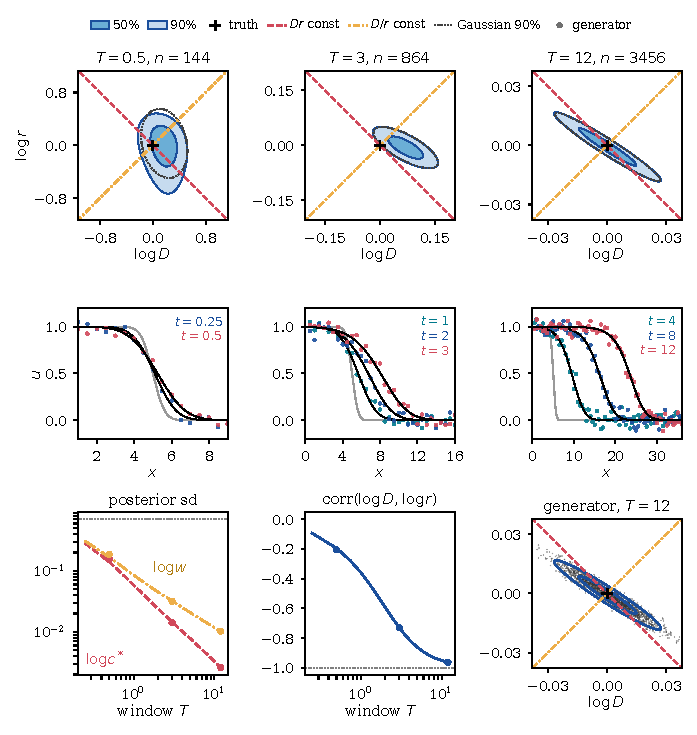
\includegraphics[width=\textwidth]{fk_posterior}
\caption{Exact posterior of $(\log D,\log r)$ for the Fisher Kolmogorov equation with $D=r=1$ and three nested observation windows $[0,T]$ with $n$ values; the axis scales differ. Top: $50$ and $90$ percent highest posterior density regions, the truth, the curves $Dr=\mathrm{const}$ (front speed) and $D/r=\mathrm{const}$ (front width) through it, and the $90$ percent region of the Gaussian approximation at the posterior mode (dotted). Middle: data (dots), solution at the posterior mean (black) and initial condition (gray). Bottom: posterior standard deviations of $\log c^*$ and $\log w$, with $c^*=2\sqrt{rD}$ and $w=\sqrt{D/r}$, and correlation of $(\log D,\log r)$ from the linearization at the truth as the window grows, with the exact values at the three windows (dots) and the prior standard deviation of $\log c^*$ and $\log w$ (dotted line); and $2000$ draws of a generator trained on $20000$ simulations, with the exact contours, for $T=12$.}
\label{fig:fk_posterior}
\end{figure}

\begin{table}[t]\centering\small
\caption{Exact posterior of $(\log D,\log r)$ by observation window: standard deviations $\sigma_D$ and $\sigma_r$ of $\log D$ and $\log r$, their correlation $\rho$, the ratio of the lengths of the principal axes of the contours, the angle of the long axis from the $\log D$ axis in degrees ($135$ is the curve $Dr=\mathrm{const}$ and $45$ the curve $D/r=\mathrm{const}$), and the standard deviations $\sigma_c$ and $\sigma_w$ of $\log c^*$ and $\log w$. The prior standard deviation of $\log D$ and $\log r$ is $1$.}\label{tab:fk_posterior}
\begin{tabular}{rrrrrrrr}
\toprule
$T$ & $\sigma_D$ & $\sigma_r$ & $\rho$ & ratio & angle & $\sigma_c$ & $\sigma_w$\\
\midrule
$0.5$ & $0.170$ & $0.298$ & $-0.21$ & $1.8$ & $100$ & $0.156$ & $0.186$\\
$3$ & $0.0412$ & $0.0263$ & $-0.73$ & $2.9$ & $151$ & $0.0142$ & $0.0315$\\
$12$ & $0.0125$ & $0.0081$ & $-0.96$ & $8.1$ & $147$ & $0.0026$ & $0.0103$\\
\bottomrule
\end{tabular}
\end{table}


\section{Two dimensional Navier Stokes on the torus}

In two dimensions the vorticity $\omega = \partial_1u_2-\partial_2u_1$ satisfies
\[
\partial_t\omega+u\cdot\nabla\omega = \nu\Delta\omega+\mathrm{curl}\,f,\qquad u = \nabla^\perp\Delta^{-1}\omega.
\]
The enstrophy $\int\omega^2$ is nonincreasing without forcing, which gives global regularity. The inverse problem of recovering $\omega(0)$ from noisy observations of $\omega(T)$ inherits the logarithmic instability of the heat equation at high frequencies, but the nonlinearity transfers energy between modes, so that information about one mode is partially encoded in others, and the posterior is no longer diagonal, as the computed example of Section~\ref{sec:simns2d} shows. As in the linear case, the posterior concentrates on large scale vortex structures and leaves small scales close to the prior in that example (Figure~\ref{fig:ns2d_posterior}). The theorems are proved for a different observation scheme. When the observations are spread over space and time starting at time zero, the information operator differs from that of the heat equation by a compact operator, smooth functionals of the state at a fixed later time have Gaussian limits at the rate $N^{-1/2}$ by the delta method, the energy and the circulation around a loop being examples, and credible bands for the trajectory have asymptotically exact coverage~\cite{konennickl2026}. The posterior can be computed by a generator trained on simulations, but the accuracy that the Gaussian statements need from the generator is a hypothesis and not a theorem (Proposition~\ref{prop:bvm_generators}). In the nonlinear experiment of Section~\ref{m:sec:expns}, a six mode truncation of the vorticity equation observed at $80$ points of space and time, a generator with an identity head trained on simulations from the prior stayed about one posterior standard deviation from a Metropolis reference as the number of simulations grew, and a generator trained near a preliminary estimate, with its residuals centered and rescaled, came to about $0.07$ posterior standard deviations~\cite{polsonsokolov2026manifold}. That is the accuracy of the Laplace approximation at the posterior mode, within the Monte Carlo error of the reference. The case for the generator in this experiment is amortization, not accuracy.

\section{History: filtering, calibration and assimilation}

Bayesian inference for dynamical systems has a long history in statistics and in the geosciences, developed largely independently. Carlin, Polson and Stoffer~\cite{cps1992} introduced Gibbs sampling for nonlinear and non Gaussian state space models. Polson and Roberts~\cite{polsonroberts1994} gave Bayes factors for diffusions observed at discrete times. Polson and Stroud developed simulation based inference for derivative pricing models, and the practical filter of Polson, Stroud and M\"uller~\cite{psm2008} addressed sequential parameter learning. Kennedy and O'Hagan~\cite{kennedyohagan2001} formalized the calibration of computer models with Gaussian process emulators and a model discrepancy term, and Higdon and coauthors extended the approach to high dimensional outputs. In meteorology, four dimensional variational assimilation computes the maximum a posteriori initial condition for a Gaussian prior and likelihood using an adjoint model, and Evensen's ensemble Kalman filter~\cite{evensen1994} propagates an ensemble of states through the forecast model and updates it linearly. In the language of this book, four dimensional variational assimilation is the mode of the posterior on the solution manifold, the ensemble Kalman filter is an affine transport approximation to the posterior (Chapter~\ref{ch:gbc}), and generative Bayesian computation is its nonlinear completion.

\section{Gaussian measures on function spaces}

The priors of this chapter are Gaussian measures on infinite dimensional spaces. Let $\mu = N(0,\mathcal{C})$ be a centered Gaussian measure on a separable Hilbert space $H$ with trace class covariance $\mathcal{C}$. Its Cameron Martin space is $E = \mathcal{C}^{1/2}H$ with norm $\|h\|_E = \|\mathcal{C}^{-1/2}h\|_H$.

\begin{theorem}[Cameron Martin, Feldman and H\'ajek]
\label{thm:cameron_martin}
The shifted measure $\mu(\cdot-h)$ is equivalent to $\mu$ if $h\in E$ and mutually singular with it otherwise. For $h\in E$,
\[
\frac{\dd\mu(\cdot-h)}{\dd\mu}(x) = \exp\Big(\langle\mathcal{C}^{-1/2}h,\mathcal{C}^{-1/2}x\rangle-\frac12\|h\|_E^2\Big),
\]
where $\langle\mathcal{C}^{-1/2}h,\mathcal{C}^{-1/2}x\rangle$ is the Paley Wiener integral: the $L^2(\mu)$ limit of $\langle\mathcal{C}^{-1}h_n,x\rangle$ for any $h_n\in\mathcal{C}H$ with $h_n\to h$ in $E$. It is a centered Gaussian variable with variance $\|h\|_E^2$. Two Gaussian measures are either equivalent or mutually singular.
\end{theorem}

We quote the theorem without proof. The density is the Cameron Martin formula and the dichotomy is the Feldman H\'ajek theorem; both are proved in Bogachev~\cite{bogachev1998}.

The Cameron Martin space has $\mu$ measure zero in infinite dimensions: draws from the prior are rougher than the functions the prior considers typical shifts. The maximum a posteriori estimator is defined through the Onsager Machlup functional
\[
I(\theta) = \mathcal{V}(\theta;y)+\frac12\|\theta\|_E^2,\qquad\mathcal{V}(\theta;y) = \frac{1}{2\delta^2}\|y-\mathcal{G}(\theta)\|^2,
\]
whose minimizer over $E$ is the Tikhonov regularized solution with penalty given by the Cameron Martin norm. Dashti, Law, Stuart and Voss~\cite{dashti2013} proved that this minimizer is the limit of the centers of small balls of maximal posterior probability, which gives the maximum a posteriori estimator a measure theoretic meaning in infinite dimensions.

\section{Well posedness of the posterior}

\begin{theorem}[Stuart]
\label{thm:stuart_wellposed}
Let $\Pi$ be a probability measure on a separable Banach space $X$ and let $\mathcal{V}:X\times\R^m\to\R$ be continuous. Suppose that for every $r>0$ there are nondecreasing functions $M_1(r,\cdot)$ and $M_2(r,\cdot)$, with $M_2$ strictly positive, such that for all $\theta\in X$ and all $y,y_1,y_2\in\R^m$ of norm at most $r$,
\[
\begin{gathered}
\mathcal{V}(\theta;y)\geq-M_1(r,\|\theta\|),\\
|\mathcal{V}(\theta;y_1)-\mathcal{V}(\theta;y_2)|\leq M_2(r,\|\theta\|)\,\|y_1-y_2\|,
\end{gathered}
\]
and that, for every $r>0$, $e^{M_1(r,\|\theta\|)}\big(1+M_2(r,\|\theta\|)^2\big)$ is integrable under $\Pi$. Then $Z(y) = \int e^{-\mathcal{V}(\theta;y)}\Pi(\dd\theta)$ is positive and finite, the measure $\Pi^y$ with density $Z(y)^{-1}e^{-\mathcal{V}(\theta;y)}$ with respect to $\Pi$ is a probability measure, and for every $r>0$ there is $C$ such that
\[
d_{\mathrm{Hell}}\big(\Pi^y,\Pi^{y'}\big)\leq C\|y-y'\|
\]
for all $y,y'$ of norm at most $r$.
\end{theorem}

This is a special case of the well posedness theorems of Dashti and Stuart~\cite{dashti2017}. The theorem holds for data in a Banach space. For a Gaussian prior the integrability condition is checked with Fernique's theorem, which gives $\int e^{\varepsilon\|\theta\|^2}\Pi(\dd\theta)<\infty$ for small $\varepsilon>0$. The condition holds for the potential $\mathcal{V}(\theta;y) = \frac{1}{2\delta^2}\|y-\mathcal{G}(\theta)\|^2$ when $\mathcal{G}$ is continuous and grows at most polynomially in $\|\theta\|$, with $M_1 = 0$ and $M_2(r,s) = \delta^{-2}\big(r+\sup_{\|\theta\|\leq s}\|\mathcal{G}(\theta)\|\big)$.

\begin{proof}[Sketch]
Fix $r>0$ and write $M_i$ for $M_i(r,\|\theta\|)$. The lower bound gives $Z(y)\leq\int e^{M_1}\dd\Pi<\infty$. Take a point $\theta_0$ in the support of $\Pi$. By continuity and the Lipschitz bound in $y$, $\mathcal{V}$ is bounded above, uniformly for $\|y\|\leq r$, on a neighborhood of $\theta_0$, and the neighborhood has positive prior mass, so $Z(y)$ is bounded away from zero. For $a,b\geq-M$ one has $|e^{-a}-e^{-b}|\leq e^M|a-b|$ and $|e^{-a/2}-e^{-b/2}|\leq\frac12e^{M/2}|a-b|$. Hence
\[
\begin{gathered}
|Z(y)-Z(y')|\leq\|y-y'\|\int e^{M_1}M_2\,\dd\Pi,\\
\int\big(e^{-\mathcal{V}(\theta;y)/2}-e^{-\mathcal{V}(\theta;y')/2}\big)^2\,\dd\Pi\leq\frac14\|y-y'\|^2\int e^{M_1}M_2^2\,\dd\Pi,
\end{gathered}
\]
and both integrals are finite by assumption. The squared Hellinger distance is at most a constant times the sum of the second integral and $|Z(y)-Z(y')|^2$, with a constant that depends on the lower bound for $Z$, and the claim follows.
\end{proof}

The map from data to the least squares initial condition is discontinuous, since the backward heat equation is ill posed in Hadamard's sense, but the map from data to posterior is Lipschitz in the Hellinger metric. Bayesian inversion is well posed where deterministic inversion is not, because it returns a measure that spreads its mass over the directions the data cannot determine.

\section{Dimension robust sampling}\label{sec:dimrobust}

Standard random walk Metropolis algorithms degenerate as the discretization of a function space problem is refined: the acceptance rate falls to zero unless the step size shrinks with the dimension. The preconditioned Crank Nicolson proposal of Cotter, Roberts, Stuart and White~\cite{cotter2013} avoids this. With prior $N(0,\mathcal{C})$, propose
\[
\theta' = \sqrt{1-\beta^2}\,\theta+\beta\,\xi,\qquad\xi\sim N(0,\mathcal{C}),
\]
and accept with probability $\min\{1,\exp(\mathcal{V}(\theta;y)-\mathcal{V}(\theta';y))\}$. The proposal is reversible with respect to the prior, so the acceptance probability involves only the likelihood, and the algorithm is well defined on the infinite dimensional space. Hairer, Stuart and Vollmer~\cite{hairer2014} proved that for a large class of target measures its Wasserstein spectral gap is bounded below independently of the discretization, and that this gap implies a spectral gap in $L^2$. The algorithm is an instance of the general principle of this book: a Markov chain that preserves the reference measure exactly, here the Gaussian prior, and corrects only for the tilt, mirrors the structure of Gibbs conditioning, in which the reference measure is fixed and only the constraint changes.

\section{A simulated example in two dimensions}\label{sec:simns2d}

Figure~\ref{fig:ns2d} shows a pseudospectral solution of the two dimensional vorticity equation, started from ten Gaussian vortices of random sign and strength. Isolated vortices persist, vortices of opposite sign close to one another are sheared into filaments, and viscosity thins the filaments. Kraichnan, Leith and Batchelor~\cite{kraichnan1967,leith1968,batchelor1969} predicted that in two dimensions energy moves to large scales and enstrophy to small scales, a dual cascade. The lower panels of the figure show the energy and enstrophy spectra, summed over shells of the wavenumber (the caption gives the definition). They show the two directions of the dual cascade only in part within $t=5$. The energy at $k=1$ rises from $0.0265$ to $0.0315$, which viscosity alone cannot do, while the total energy falls by $11$ percent, and the share of the energy at $k\le3$ rises from $0.82$ to $0.87$, so energy moves to large scales. The share of the enstrophy at $k\ge16$ grows from $5\times10^{-7}$ to $2.4\times10^{-3}$, so some enstrophy moves to small scales, but the total enstrophy falls by $32$ percent and its mean wavenumber does not rise, from $3.9$ to $3.8$. Three times of one flow do not show an inertial range.

\begin{figure}[t]
\centering
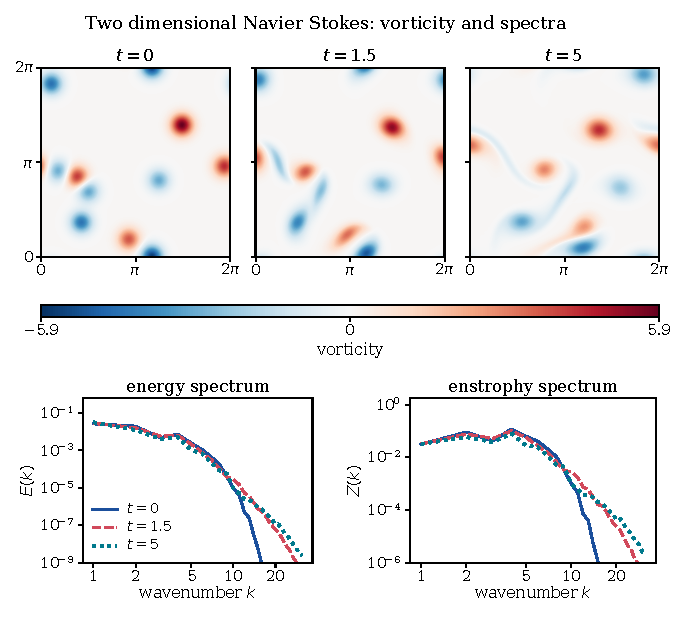
\includegraphics{ns2d}
\caption{Top: vorticity of a two dimensional Navier Stokes flow on the torus $[0,2\pi]^2$ with viscosity $\nu = 2\times10^{-3}$ at times $t = 0$, $1.5$ and $5$, started from ten Gaussian vortices of random sign. Red is positive and blue is negative vorticity (both print dark in grayscale), on one symmetric color scale for the three panels, with limits $\pm5.87$, the largest absolute value of the initial vorticity. Bottom: the energy spectrum $E(k)$ and the enstrophy spectrum $Z(k)$ per unit area at the same times, on logarithmic axes; with $\hat\omega_j$ the Fourier coefficients of the vorticity, $E(k)$ is the sum of $\frac12|\hat\omega_j|^2/|j|^2$ and $Z(k)$ the sum of $\frac12|\hat\omega_j|^2$ over the wavenumbers $j$ with $|j|$ rounded to $k$. The solution is computed by a dealiased pseudospectral method with fourth order Runge Kutta time stepping on a $96\times96$ grid.}
\label{fig:ns2d}
\end{figure}

We computed the inverse problem for a smaller flow than the one of Figure~\ref{fig:ns2d}, with a coarser grid and a larger viscosity, so that the posterior could be sampled exactly. The unknown is the initial vorticity $\omega_0=\sum_{0<|k|_\infty\le6}c_ke^{ik\cdot x}$ on $\T^2$, with $c_{-k}=\bar c_k$, which has $168$ real coefficients. The prior makes the coefficients independent and Gaussian with $\E|c_k|^2=(1+|k|^2)^{-2}$, a Mat\'ern type prior of smoothness index $1$ whose pointwise standard deviation is $1.47$. The data are the values of $\omega(T)$ at time $T=3$ at $16\times16$ equally spaced sensors, with independent Gaussian noise of standard deviation $\delta=0.25$, for viscosity $\nu=0.01$. The forward map is a dealiased pseudospectral solver with fourth order Runge Kutta steps of size $0.025$ on a $32\times32$ grid. The truth is five Gaussian vortices $a\,e^{-r^2/0.5}$, with amplitudes $a$ of both signs between $2.5$ and $6$ in absolute value, projected on the $168$ modes (Figure~\ref{fig:ns2d_posterior_data}), so that the model is correctly specified. The data were generated on a $64\times64$ grid with half the time step, not on the grid of the posterior, so that there is no inverse crime: the two solutions differ at the sensors by $0.03$ in root mean square, one ninth of $\delta$.

\begin{figure}[t]
\centering
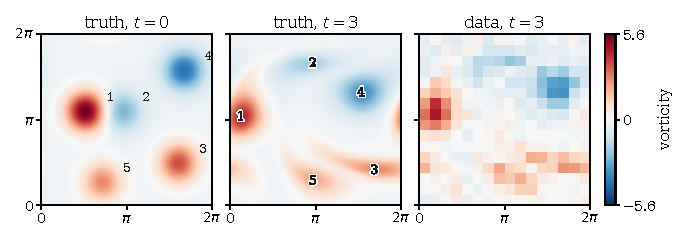
\includegraphics{ns2d_posterior_data}
\caption{Truth and data of the simulated inverse problem. Left: the initial vorticity of the truth, five Gaussian vortices numbered $1$ to $5$. Middle: the truth at the observation time $t=3$; the numbers mark where the five vortices have gone. Right: the data. One color scale for the three panels.}
\label{fig:ns2d_posterior_data}
\end{figure}

We found the maximum of the posterior density by a Levenberg Marquardt iteration, formed the Gauss Newton Hessian there, and sampled the posterior exactly by Hamiltonian Monte Carlo~\cite{duane1987,neal2011} in coordinates in which that Hessian is the identity. The gradient of the log posterior is the reverse mode derivative of the solver. Four chains were started from independent draws of the prior, and each ran $400$ warmup iterations, with the step size set by dual averaging~\cite{hoffman2014}, followed by $1000$ iterations with a random number of leapfrog steps. The mean acceptance probability was $0.77$. The largest rank normalized split $\widehat R$~\cite{vehtari2021} over the $168$ coefficients is $1.010$, and the smallest bulk effective sample size is $552$ out of $4000$ draws. The four chains reach the same posterior, and three further optimizations started from other prior draws end at the same maximum, so that we found no sign of several modes. That says nothing about regimes with a lower viscosity, a longer observation time or fewer sensors, which we did not compute. On the linear problem obtained by dropping the nonlinear term, whose posterior is Gaussian and known in closed form, the same sampler, with four chains of $300$ warmup and $600$ retained iterations, has $\widehat R\le1.009$ and reproduces the standard deviations of all $168$ coefficients to within $6$ percent, the largest of $168$ Monte Carlo errors of about $2$ percent each.

\begin{figure}[t]
\centering
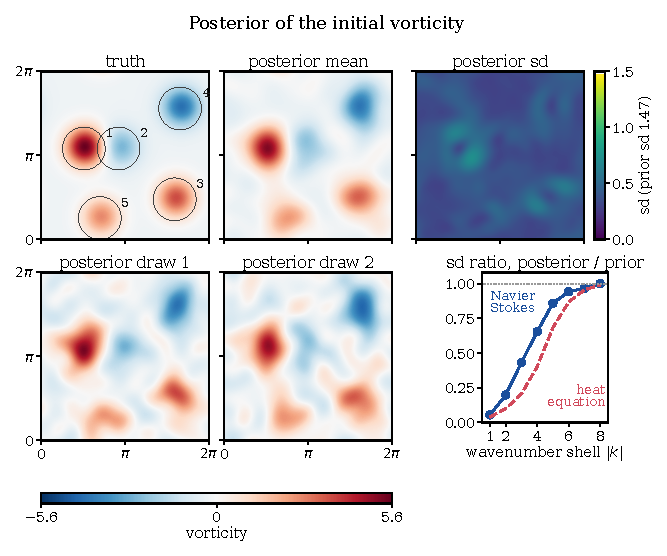
\includegraphics{ns2d_posterior}
\caption{Posterior of the initial vorticity for the data of Figure~\ref{fig:ns2d_posterior_data}, from four Hamiltonian Monte Carlo chains. Top: the truth, with the five discs of radius $0.8$ on which circulations are computed, the posterior mean, and the pointwise posterior standard deviation on a color scale from zero to the prior standard deviation $1.47$. Bottom: two posterior draws on the color scale of the truth, and the ratio of posterior to prior standard deviation of the Fourier coefficients by wavenumber shell (the square root of the ratio of the summed variances over the modes with $|k|$ rounded to $m$), for the nonlinear problem and for the problem with the nonlinear term dropped.}
\label{fig:ns2d_posterior}
\end{figure}

Figure~\ref{fig:ns2d_posterior} shows the posterior. The posterior mean recovers the five vortices, the draws differ from it in a fine scale texture that the data do not constrain, and the standard deviation of the field is at most $0.74$, against $1.47$ for the prior. By wavenumber shell, the ratio of the posterior to the prior standard deviation of the coefficients, pooled over the shell as in the caption, is $0.05$, $0.20$ and $0.43$ for $|k|=1,2,3$, $0.65$ at $|k|=4$ and $0.86$ at $|k|=5$, and at least $0.94$ for $|k|\ge6$: the large scales are learned and the small scales are left at the prior. With the nonlinear term dropped, the vorticity equation becomes the heat equation, and the same prior, sensors and noise give a diagonal posterior that learns more at every wavenumber, with ratios $0.04$, $0.10$, $0.20$, $0.40$ and $0.68$ for $|k|=1,\dots,5$. The nonlinear posterior is not diagonal: $158$ of the $14028$ pairs of coefficients have a posterior correlation above $0.3$ in absolute value, and the largest is $0.67$.

\begin{table}[t]\centering\footnotesize\setlength{\tabcolsep}{5pt}
\caption{Posterior mean and standard deviation (sd) of the energy and of the circulations of the initial vorticity. The prior standard deviation is $14.3$ for the energy, estimated from $20000$ prior draws, and $2.36$ for every circulation. The circulation is the integral of $\omega_0$ over the disc of radius $0.8$ around vortex $j$. The position error is the root mean square distance, over posterior draws, between the location of the extremum of $\omega_0$ in that disc and its location in the truth; under the prior it is between $0.72$ and $0.73$ for every vortex. The elongation is the ratio of the principal axes of the region in which vortex $j$, advected to $t=3$ separately by the velocity of the whole field, exceeds a fifth of its maximum; it is $1$ at $t=0$.}\label{tab:ns2d_posterior}
\begin{tabular}{@{}lrrrrr@{}}
\toprule
Functional & Truth & Mean & Sd & Position error & Elongation\\
\midrule
Energy & $12.62$ & $13.03$ & $0.42$ & & \\
Circulation 1 & $5.88$ & $5.78$ & $0.19$ & $0.14$ & $1.33$\\
Circulation 2 & $-2.37$ & $-2.39$ & $0.24$ & $0.32$ & $2.43$\\
Circulation 3 & $4.02$ & $3.85$ & $0.19$ & $0.20$ & $4.52$\\
Circulation 4 & $-5.06$ & $-5.03$ & $0.16$ & $0.26$ & $1.31$\\
Circulation 5 & $2.88$ & $2.70$ & $0.16$ & $0.26$ & $2.17$\\
\bottomrule
\end{tabular}
\end{table}

Table~\ref{tab:ns2d_posterior} gives the posterior of the energy $\frac12\int_{\T^2}|u_0|^2\dd x$ of the initial velocity and of the circulations on the discs of Figure~\ref{fig:ns2d_posterior}. The standard deviation of the energy is $3$ percent of its prior value and those of the circulations are $7$ to $10$ percent of theirs. The truth is within $1.2$ posterior standard deviations of the posterior mean for each of the six, and the posterior of the energy is close to normal, with skewness $0.10$ and excess kurtosis $-0.03$. We repeated the computation with the same noise draw rescaled to $\delta=0.5$ and $\delta=0.125$, with $300$ warmup and $600$ retained iterations per chain, $\widehat R\le1.03$ and a bulk effective sample size of at least $196$ for the coordinates; the Monte Carlo error of each standard deviation of a functional below is $2$ to $4$ percent. The standard deviation of the energy is $0.83$, $0.42$ and $0.21$ for $\delta=0.5$, $0.25$ and $0.125$, proportional to $\delta$ within $2$ percent, and those of the circulations of vortices 1, 3, 4 and 5 scale as $\delta^s$ over the same range with $s$ between $0.90$ and $1.07$. The circulation of vortex 2, the weakest, scales as $\delta^{0.73}$, and the point value of $\omega_0$ at the center of vortex 1, which depends on small scales, as $\delta^{0.68}$. A standard deviation proportional to $\delta$, together with a nearly normal posterior, is what a Bernstein von Mises theorem leads one to expect of a smooth functional. In this experiment the energy has both. One experiment says nothing about rates. The Gaussian approximation at the maximum of the posterior gives standard deviations of these six functionals that are $4$ to $11$ percent too small, and the importance weights of its draws have an effective sample size of $0.9$ percent, so that as a measure on $\R^{168}$ it is not close to the posterior.

The five vortices are not determined equally well. Advected separately by the velocity of the whole field, vortices 3 and 5 are drawn by $t=3$ into thin arcs and vortex 2 into a flat band, while vortices 1 and 4 stay compact (Table~\ref{tab:ns2d_posterior}). The standard deviation of the circulation of vortex 2 is the largest of the five, and so is the error of its position. But vortex 3, the most elongated, has the circulation standard deviation of the compact vortex 1, and vortex 5, which is also drawn into an arc, has a circulation standard deviation as small as that of the compact vortex 4. Vortex 2 is also the weakest of the five, so that this experiment shows no clear effect of filamentation on how well a vortex is determined.


\section*{Exercises}
\begin{enumerate}
\item In the heat equation sequence model, derive the posterior mean and variance of $\theta_k$.
\item Show that the functional $L\theta = \theta_1$ satisfies the summability condition of Theorem~\ref{thm:heat_rates} and compute its asymptotic variance.
\item Prove that the preconditioned Crank Nicolson proposal is reversible with respect to $N(0,\mathcal{C})$.
\item Show that a traveling front $U(x-ct)$ of the Fisher Kolmogorov equation satisfies $DU''+cU'+rU(1-U) = 0$, and that rescaling the variable by $\sqrt{D/r}$ leaves the single parameter $c/\sqrt{rD}$.
\item Compute the Cameron Martin norm of a smooth function $h$ with $h(0) = 0$ under the Brownian motion prior on $[0,1]$.
\end{enumerate}


\section*{Notes}

The generative computation on the solution manifold is from our paper~\cite{polsonsokolov2026manifold}. Our earlier paper~\cite{polsonsokolov2026ns} treats the discretized Navier Stokes equations as a state space model and learns parameters by particle learning.

\chapter{The Boundary of the Manifold: Blowup, Turbulence and Steady Flows}
\label{ch:boundary}

\section{Where the derivation stops}

The strong derivations of Chapters~\ref{ch:kinetic} and~\ref{ch:hydro} are valid for as long as the limiting equations have smooth solutions. In three dimensions nobody knows how long that is. The weak derivation of Golse and Saint Raymond~\cite{golsesaintraymond2004} needs no smoothness and ends in Leray solutions of the limiting fluid equations, but Leray solutions are not known to be unique, so it does not select a solution once smoothness may fail. The solution manifold of Chapter~\ref{ch:nsinference} therefore has a boundary: the set of initial conditions whose trajectories cease to be smooth, if it is not empty, and the regime of fully developed turbulence, in which solutions are smooth in principle but so rough in practice that only statistical descriptions are meaningful.

\section{Leray and the regularity problem}

In 1934 Jean Leray~\cite{leray1934} proved that for every initial velocity of finite energy in $\R^3$ there is a global weak solution of the Navier Stokes equations satisfying the energy inequality
\[
\frac12\|u(t)\|_{L^2}^2+\nu\int_0^t\|\nabla u(s)\|_{L^2}^2\dd s\leq\frac12\|u(0)\|_{L^2}^2.
\]
He called such solutions turbulent solutions, conjecturing that singularities might be the mathematical origin of turbulence, and he proposed a mechanism: a self similar solution
\[
u(t,x) = \frac{1}{\sqrt{2a(T^*-t)}}\,U\Big(\frac{x}{\sqrt{2a(T^*-t)}}\Big)
\]
whose profile $U$ solves a stationary elliptic system. Ne\v{c}as, R\r{u}\v{z}i\v{c}ka and \v{S}ver\'ak~\cite{necas1996} proved in 1996 that no nontrivial profile in $L^3(\R^3)$ exists, and Tsai~\cite{tsai1998} extended this to profiles in $L^q(\R^3)$ for every $q>3$ and to self similar solutions that satisfy the local energy estimates. Escauriaza, Seregin and \v{S}ver\'ak~\cite{ess2003} showed in 2003 that a solution of the unforced equations bounded in $L^\infty_tL^3_x$ cannot blow up, so any singularity must make the critical $L^3$ norm unbounded.

The partial regularity theorem of Caffarelli, Kohn and Nirenberg~\cite{ckn1982} shows that for suitable weak solutions the singular set has one dimensional parabolic Hausdorff measure zero, hence parabolic Hausdorff dimension at most one: singularities, if they exist, are rare in space time. The Beale, Kato and Majda criterion~\cite{bkm1984}, proved for Euler and valid also for Navier Stokes, shows that a smooth solution on $[0,T^*)$ blows up at $T^*$ if and only if, for the vorticity $\omega=\operatorname{curl}u$,
\[
\int_0^{T^*}\|\omega(t)\|_{L^\infty}\dd t = \infty.
\]

Tao~\cite{tao2016} constructed finite time blowup for an averaged version of the Navier Stokes equations that obeys the same energy identity, showing that energy methods alone cannot prove regularity. Buckmaster and Vicol~\cite{buckmastervicol2019} proved nonuniqueness of weak solutions with finite energy by convex integration; these solutions are not required to satisfy the energy inequality, so they are not Leray solutions. Albritton, Bru\'e and Colombo~\cite{abc2022} proved nonuniqueness of Leray solutions with a suitably chosen forcing. For the Euler equations, Elgindi~\cite{elgindi2021} proved finite time singularity formation for $C^{1,\alpha}$ velocity fields for some small $\alpha>0$, and Chen and Hou~\cite{chenhou2022,chenhou2025} gave a computer assisted proof of stable, nearly self similar blowup of the axisymmetric equations for smooth data of finite energy in the presence of a boundary, confirming the scenario found numerically by Luo and Hou~\cite{luohou2014}. The regularity question for smooth data in $\R^3$ without boundary remains open.

\section{Blowup as a parameter}\label{sec:blowup_param}

From the inferential point of view, the blowup time is a functional of the initial condition, possibly infinite, and its posterior is a well defined object. Self similar or type I blowup predicts $\|\omega(t)\|_{L^\infty}\approx c/(T^*-t)$ near the singular time, the rate that makes the Beale Kato Majda integral diverge logarithmically. Hence the reciprocal $y(t) = 1/\|\omega(t)\|_{L^\infty}$ is approximately linear in $t$ and vanishes at $T^*$.

\begin{proposition}[Posterior for the blowup time]
\label{prop:blowup_time}
Suppose $y_j = a+bt_j+\xi_j$ for $j = 1,\dots,m$, with $\xi_j\sim N(0,\sigma^2)$ independent and $\sigma$ known. Let $X$ be the $m\times2$ matrix with rows $(1,t_j)$, let $(c_{\cdot\cdot}) = (X^\top X)^{-1}$, and let $(\hat a,\hat b)$ be the least squares estimate. Take the prior flat on $\R^2$ and set $T^* = -a/b$ if $b<0$ and $T^* = +\infty$ if $b\geq0$. The posterior of $(a,b)$ is Gaussian with mean $(\hat a,\hat b)$ and covariance $\sigma^2(X^\top X)^{-1}$, the posterior probability of no blowup is
\[
\P(T^* = +\infty\mid\text{data}) = \P(b\geq0\mid\text{data}) = \Phi\Big(\frac{\hat b}{\sigma\sqrt{c_{bb}}}\Big),
\]
where $\Phi$ is the standard normal distribution function, and on $\{b<0\}$ the posterior of $T^*$ is that of $-a/b$, a ratio of correlated Gaussians. The Fieller set~\cite{fieller1954}
\[
F_\gamma = \Big\{T:\frac{(\hat a+\hat bT)^2}{\sigma^2(c_{aa}+2c_{ab}T+c_{bb}T^2)}\leq z_{1-\gamma/2}^2\Big\},
\]
with $z_{1-\gamma/2} = \Phi^{-1}(1-\gamma/2)$, contains the zero $-a/b$ of the line with sampling probability exactly $1-\gamma$, for every $(a,b)$ with $b\neq0$, and it is bounded if and only if $\hat b^2>z_{1-\gamma/2}^2\sigma^2c_{bb}$.
\end{proposition}

\begin{proof}
The posterior is the standard result for the Gaussian linear model with a flat prior, and the marginal of $b$ is $N(\hat b,\sigma^2c_{bb})$, which gives the probability of no blowup. For fixed $T$ put $q(T) = c_{aa}+2c_{ab}T+c_{bb}T^2$, which is positive because $(c_{\cdot\cdot})$ is positive definite. Under the sampling law $\hat a+\hat bT$ is $N(a+bT,\sigma^2q(T))$, so at $T = -a/b$, when $b\neq0$, the statistic $(\hat a+\hat bT)^2/(\sigma^2q(T))$ has the $\chi^2_1$ law and does not exceed $z_{1-\gamma/2}^2$ with probability $1-\gamma$. This is the coverage. The set $F_\gamma$ is $\{Q\leq0\}$ for the quadratic $Q(T) = (\hat a+\hat bT)^2-z_{1-\gamma/2}^2\sigma^2q(T)$. If its leading coefficient $\hat b^2-z_{1-\gamma/2}^2\sigma^2c_{bb}$ is positive, then $\hat b\neq0$ and $Q(-\hat a/\hat b) = -z_{1-\gamma/2}^2\sigma^2q(-\hat a/\hat b)<0$, so $F_\gamma$ is a bounded interval. If the leading coefficient is negative, then $Q<0$ outside a bounded set. If it is zero, then $\hat b\neq0$, $Q$ is affine, and the same value shows that $\{Q\leq0\}$ is not empty, so it is a half line or $\R$. In the last two cases $F_\gamma$ is unbounded.
\end{proof}

The set $F_\gamma$ has exact coverage as a confidence set. As a posterior statement it is conservative, but only when the fitted line is close to zero. Whitening the posterior shows that the posterior probability that $-a/b$ lies in $F_\gamma$ depends on the data only through $r = \|X(\hat a,\hat b)^\top\|/\sigma$, the norm of the fitted values in units of $\sigma$. It equals $1$ for $r\leq z_{1-\gamma/2}$ and tends to $1-\gamma$ as $r\to\infty$; for $\gamma = 0.05$ numerical integration gives $0.982$, $0.954$ and $0.9505$ at $r = 2$, $2.5$ and $3$. Once the fitted line is more than a few noise standard deviations from zero, $F_\gamma$ is therefore a credible set of level $1-\gamma$ to good approximation, whether or not the slope is well determined.

The proposition shows that the evidence for a finite singular time in a computed solution is a statistical statement, the boundedness of a Fieller set, and that the natural summary of a simulation at fixed resolution is a posterior distribution over $T^*$ that places mass on $+\infty$ when the slope is not well determined. For $\hat b<0$ the two statements agree: $F_\gamma$ is bounded exactly when $\P(b\geq0\mid\text{data})<\gamma/2$. The model treats the error of the solver as independent Gaussian noise of constant variance on $y$, and this is its main limitation. The discretization error is deterministic, it is correlated in time, and it grows as the solution approaches the singular time. A fuller treatment puts a prior on the exponent as well, $\|\omega\|_\infty\approx c(T^*-t)^{-\theta}$, whose posterior distinguishes type I from type II scenarios, and replaces the independent noise by a model of the discretization error.

For forced equations blowup has been proved in several settings. For every $\beta<\frac12$, C\'ordoba and Mart\'inez Zoroa~\cite{cordoba2023} constructed solutions of the forced three dimensional Euler equations on $\R^3$, with a force bounded in $C^{1,\beta}\cap L^2$ uniformly in time, for which $\int_0^t\|\nabla u\|_{L^\infty}\dd s\to\infty$ as $t$ approaches a finite time. They also showed~\cite{cordoba2024} that the two dimensional incompressible porous media equation with a compactly supported source, smooth in space uniformly in time, has a smooth finite energy solution that becomes singular at a finite time. With Zheng they proved~\cite{cordoba2026} that the forced hypodissipative Navier Stokes equations on $\R^3$ with positive viscosity have solutions of finite energy, smooth in space before a finite time and with $\int_0^t\|\nabla u\|_{L^\infty}\dd s\to\infty$ as $t$ approaches it, for a force in $L^1_tC^{1,\beta}_x\cap L^\infty_tL^2_x$ with some $\beta>0$ and dissipation exponents $0\leq\alpha<(11-4\sqrt7)/9\approx0.046$ in the notation of Section~\ref{sec:hypodiss}. Alp\"oge, Buckmaster and Coiculescu~\cite{alpoge2026} proved finite time blowup for the porous media equation on the torus $\T^2$ with a force that is smooth in space and time, and announce analogous results of Alp\"oge and Buckmaster, with proofs in preparation, for the forced two dimensional inviscid Boussinesq equations and for the forced three dimensional Euler equations among axisymmetric solutions with swirl. None of these results concerns the Navier Stokes equations themselves, $\alpha = 1$.

For forced problems the forcing is itself an unknown function, and the question of whether a smooth forcing can drive a given flow to blowup is an inverse problem. One possible prior favors sparsity, a few localized forcing modes rather than many. The horseshoe prior of Carvalho, Polson and Scott~\cite{carvalho2010}, treated in Chapter~\ref{ch:mixtures}, shrinks small coefficients strongly and leaves large ones nearly unshrunk, which is the behavior wanted here. We have not tested it on this problem and offer it as a proposal.

\section{Hypodissipation and the Mat\'ern connection}\label{sec:hypodiss}

Replacing $\nu\Delta$ by $-\nu(-\Delta)^\alpha$ gives the hypodissipative ($\alpha<1$) or hyperdissipative ($\alpha>1$) Navier Stokes equations. J.\,L.~Lions~\cite{lions1969} showed in 1969 that for $\alpha\geq5/4$ in three dimensions smooth solutions exist globally: the dissipation then controls the nonlinearity at the critical scaling, since the energy is critical when $\alpha = 5/4$. Tao~\cite{tao2009} improved this by a logarithm. For $\alpha<5/4$ and no forcing, whether smooth solutions exist globally is open, as it is for the classical case $\alpha = 1$; with forcing, blowup has been proved for small $\alpha$, as described in Section~\ref{sec:blowup_param}.

The operator $(\kappa^2-\Delta)^\alpha$ is the precision operator of the Mat\'ern Gaussian field of Chapter~\ref{ch:mixtures}. Consider the linear hypodissipative Stokes system on the torus, driven by space time white noise projected onto solenoidal fields. Its stationary law is Gaussian and supported on solenoidal fields, with spectral density proportional to $|k|^{-2\alpha}$ times the projection onto the plane orthogonal to $k$, a Mat\'ern law with $\kappa = 0$, and in three dimensions its shell summed energy spectrum is proportional to $k^{2-2\alpha}$. In this linear model the dissipation exponent of the dynamics and the smoothness parameter of the stationary statistics are the same parameter, and a measured spectrum carries information about $\alpha$. The gamma mixture representation of the Mat\'ern class suggests that a posterior for $\alpha$ can be computed by data augmentation, which we have not implemented. The inference does not extend to the nonlinear equations. In the inertial range the argument of Section~\ref{sec:k41} gives the spectrum $k^{-5/3}$ for every $\alpha$, since it uses only the dissipation rate and the wavenumber, and the linear model would read this spectrum as $\alpha = 11/6$, which lies outside the range $\alpha<5/4$ where regularity is open.

\section{Turbulence: Kolmogorov 1941}\label{sec:k41}

Richardson's cascade picture of 1922~\cite{richardson1922}, in which large eddies break into smaller ones until viscosity dissipates them, was made quantitative by Kolmogorov in 1941~\cite{kolmogorov1941a,kolmogorov1941b}. Assume that at high Reynolds number the statistics of velocity increments $\delta u(\ell) = u(x+\ell)-u(x)$ at scales $\ell$ in an inertial range, far from both the forcing scale and the viscous scale, are homogeneous, isotropic and determined by the mean energy dissipation rate per unit mass $\varepsilon$ alone. Dimensional analysis then gives the structure functions $S_p(\ell) = \E|\delta u(\ell)|^p\propto(\varepsilon\ell)^{p/3}$ and the energy spectrum
\[
E(k) = C_K\,\varepsilon^{2/3}k^{-5/3}.
\]
Kolmogorov derived an exact relation for the third order longitudinal structure function, and from it the four fifths law. It is a statement of physics and not a theorem about solutions of the Navier Stokes equations, because its hypotheses are those of the physical picture. The flow is statistically stationary, homogeneous and isotropic, it is maintained by a forcing at a scale $L_f$, and the mean dissipation $\varepsilon = \nu\E|\nabla u|^2$, which equals the mean power injected by the forcing, remains positive as $\nu\to0$. Whether solutions of the Navier Stokes equations behave in this way is the question of anomalous dissipation, which is open (Section~\ref{sec:onsager_conjecture}).

For the increments of such a flow, the Navier Stokes equations with forcing $f$ give the K\'arm\'an Howarth Monin balance
\[
\nabla_\ell\cdot\E\big[|\delta u|^2\delta u\big] = 2\nu\Delta_\ell\E|\delta u|^2-4\varepsilon+2\E[\delta u\cdot\delta f],
\]
where $\delta f$ is the increment of the forcing. For $\ell$ much smaller than $L_f$ the last term is negligible. Isotropy and incompressibility reduce the balance to a relation between the longitudinal structure functions $S_2^\parallel(\ell) = \E[(\delta u_\parallel)^2]$ and $S_3^\parallel(\ell) = \E[(\delta u_\parallel)^3]$, where $\delta u_\parallel$ is the component of the increment along the separation,
\begin{equation}\label{eq:kh_exact}
S_3^\parallel(\ell) = -\frac45\varepsilon\ell+6\nu\,\partial_\ell S_2^\parallel(\ell).
\end{equation}
The balance and its isotropic reduction are derived in Frisch~\cite{frisch1995}. In the inertial range $\eta\ll\ell\ll L_f$, where $\eta = (\nu^3/\varepsilon)^{1/4}$ is the Kolmogorov scale, $S_2^\parallel\propto(\varepsilon\ell)^{2/3}$, so the viscous term is smaller than the first term by a factor of order $(\eta/\ell)^{4/3}$, and what remains is Kolmogorov's four fifths law
\begin{equation}\label{eq:fourfifths}
\E\big[(\delta u_\parallel(\ell))^3\big] = -\frac45\varepsilon\ell.
\end{equation}
The law is one of the few exact results about three dimensional turbulence. The four thirds law $\E[\delta u_\parallel|\delta u|^2] = -\frac43\varepsilon\ell$ and the K\'arm\'an Howarth equation are others~\cite{frisch1995}.

Rigorous versions need hypotheses that the physical statement does not make. Duchon and Robert~\cite{duchonrobert2000} showed that a weak solution of the Euler equations in $L^3$ on the torus satisfies a local energy balance with a defect distribution $D$. When the solution is the strong $L^3$ limit of Leray solutions $u^\nu$ of the Navier Stokes equations, $D$ is the distributional limit of $\nu|\nabla u^\nu|^2$ plus the nonnegative defect of $u^\nu$ itself, so $D\geq0$. If $\ell^{-1}\delta u_\parallel|\delta u|^2$, averaged over the direction of the separation, converges in the sense of distributions as $\ell\to0$, then $D$ is $-\frac34$ times the limit: this is a local four thirds law. Eyink~\cite{eyink2003} showed that under the same kind of assumption $\ell^{-1}(\delta u_\parallel)^3$, averaged over directions, converges to $-\frac45D$, which is the four fifths law in the same local sense, and that the mixed moment with one longitudinal and two transverse increments gives the four fifteenths law. Bedrossian, Coti Zelati, Punshon Smith and Weber~\cite{bcpw2019} proved an averaged four fifths law, averaged over space and over the direction of the separation, for stationary martingale solutions of the Navier Stokes equations on $\T^3$ forced by noise that is white in time and colored in space. Their only assumption on the solutions is weak anomalous dissipation, $\nu\E\|u\|_{L^2}^2\to0$ as $\nu\to0$, and the law holds uniformly for $\ell_D(\nu)\leq\ell\leq\ell_I$ in the limit $\nu\to0$ followed by $\ell_I\to0$, where $\ell_D(\nu)\to0$. Whether solutions satisfying this assumption exist is open.

Kolmogorov~\cite{kolmogorov1962} and Obukhov~\cite{obukhov1962}, in the same issue of the \emph{Journal of Fluid Mechanics}, revised the theory in 1962 to account for intermittency, the fluctuation of the local dissipation rate, and proposed that the dissipation averaged over a ball of radius $\ell$ is lognormal with a variance growing like $\log(L/\ell)$. The refined theory predicts structure function exponents $\zeta_p$ that deviate from $p/3$, as observed. It is a curious coincidence, though a natural one from the point of view of Chapter~\ref{ch:mixtures}, that Thorin's original motivation~\cite{thorin1977} for generalized Gamma convolutions was to prove that the lognormal law is infinitely divisible: the dissipation field of K62 is a multiplicative cascade, an infinite product of independent factors, and its logarithm is an infinite sum. Multifractal models such as that of She and Leveque~\cite{sheleveque1994}, $\zeta_p = \frac p9+2\big(1-(\frac23)^{p/3}\big)$, are log infinitely divisible cascades in this sense.

\section{Onsager's conjecture}\label{sec:onsager_conjecture}

Onsager~\cite{onsager1949} observed in 1949 that a constant energy flux $\varepsilon$ through scale $\ell$, of order $|\delta u|^3/\ell$, requires $|\delta u|\sim(\varepsilon\ell)^{1/3}$, the scaling of the four fifths law. The velocity field of turbulence at zero viscosity therefore cannot be more regular than H\"older continuous of exponent one third, since otherwise the flux would vanish as $\ell\to0$ and energy would be conserved. An unpublished note of 1945 to C.\,C.~Lin contains an identity analogous to the four fifths law, and Eyink and Sreenivasan~\cite{eyinksreenivasan2006} infer that it was the basis of the claim. Onsager conjectured that weak solutions of the Euler equations conserve energy if their H\"older exponent exceeds one third, and that dissipative solutions exist with any exponent below one third.

\begin{theorem}[Constantin, E and Titi; Isett]
\label{thm:onsager}
Let $T>0$ and consider weak solutions of the incompressible Euler equations on $[0,T]\times\T^3$, in the sense of distributions. If $u\in L^3(0,T;C^{0,\beta}(\T^3))$ with $\beta>\frac13$, then $\int_{\T^3}|u(x,t)|^2\dd x$ is constant for almost every $t$. For every $\beta<\frac13$ there is a weak solution $u\in C([0,T];C^{0,\beta}(\T^3))$ whose energy $\int_{\T^3}|u(x,t)|^2\dd x$ is not constant in $t$.
\end{theorem}

We quote both halves without proof. The first half was proved by Constantin, E and Titi~\cite{cet1994} in 1994 by a commutator estimate on mollified equations, and Bardos and Titi~\cite{bardostiti2018} proved it in a bounded domain $\Omega$ with $C^2$ boundary, for solutions with $u\cdot n = 0$ on $\partial\Omega$ that lie in $L^3(0,T;C^{0,\beta}(\overline\Omega))$ with $\beta>\frac13$. The second half was proved by Isett in 2018~\cite{isett2018}, completing a program of convex integration begun by De Lellis and Sz\'ekelyhidi~\cite{delellisszekelyhidi2009}. Buckmaster, De Lellis, Sz\'ekelyhidi and Vicol~\cite{bdsv2019} showed that for every $\beta<\frac13$ and every smooth positive energy profile $e(t)$ there is a weak solution in $C^\beta([0,T]\times\T^3)$ with energy $e(t)$, so that a decreasing profile gives strictly dissipative solutions. Onsager's threshold is now a theorem, and anomalous dissipation is mathematically possible. Whether it is the mechanism of real turbulence, that is, whether vanishing viscosity limits of Navier Stokes solutions dissipate energy at a positive rate, remains open.

From the inferential standpoint, the dissipation rate $\varepsilon$, the Kolmogorov constant $C_K$, and the exponents $\zeta_p$ are parameters of a statistical model for velocity increments, and their posterior distributions given measured increments are the natural objects. The four fifths law gives a moment condition for $\varepsilon$; the higher structure functions inform the intermittency parameters. A Bayesian analysis of turbulence data is therefore a mixture model problem, and the scale mixture machinery of Chapter~\ref{ch:mixtures} applies directly. Conditionally on the local dissipation the increments cannot be Gaussian, since a centered Gaussian has zero third moment. The model of Section~\ref{sec:infer_dissipation} instead writes the increment as $(\varepsilon_\ell\ell)^{1/3}Z$ with $Z$ skewed, and the local dissipation $\varepsilon_\ell$ is lognormal or log infinitely divisible.

\section{Steady flows and flow MRI}

At the other end of the spectrum from turbulence lie steady laminar flows,
\[
u\cdot\nabla u+\nabla p = \nu\Delta u,\qquad\nabla\cdot u = 0\quad\text{in }\Omega,\qquad u = g\ \text{on }\partial\Omega.
\]
In medical and engineering applications the domain $\Omega$, the boundary data $g$ and the viscosity are partly unknown, and the velocity is measured, noisily and at limited resolution, by magnetic resonance velocimetry. Kontogiannis, Elgersma, Sederman and Juniper~\cite{kontogiannis2025} formulated this as a Bayesian inverse problem in which the unknowns are the inlet velocity, the outlet conditions, the shape of the boundary, represented implicitly by a viscous signed distance function, and the viscosity, and computed the maximum a posteriori estimate by an adjoint based iteration. A quasi Newton (BFGS) approximation of the inverse Hessian, which is the posterior covariance of the Laplace approximation, accelerates the iteration. The reconstructed velocity field satisfies the Navier Stokes equations by construction, and quantities that are difficult to measure, such as the pressure and the wall shear stress, follow from the reconstruction. The method was tested on magnetic resonance data of a steady flow through a physical model of an aortic arch. Estimating the posterior uncertainty from the approximate covariance is left to future work in that paper.

In the language of this book, the boundary data play the role of the initial condition, the solution manifold is the set of steady solutions indexed by boundary data and shape, and the reconstruction is projection onto that manifold. Two extensions are natural, and neither has been carried out for flow MRI. The first uses the adjoint computation as a summary statistic, in the manner of Chapter~\ref{ch:manifold}. The gradient of the data misfit at a fixed reference state costs one adjoint solve per dataset, once the forward solve at the reference state is done, whereas the maximum a posteriori estimate needs a forward and an adjoint solve at every step of the optimization. A generator trained on simulations to map this statistic to posterior draws could capture non Gaussian features of the posterior that the Laplace approximation misses. The second is that the shape uncertainty, which is non Gaussian because shapes form a manifold, could be represented by transport maps of the kind discussed in Chapter~\ref{ch:gbc}.

\section{The boundary as a modeling frontier}

The three regimes of this chapter differ in their mathematics but share an inferential structure. In each, the deterministic solution manifold is either incompletely understood or practically inaccessible at the relevant resolution, and statistical modeling enters not as a convenience but as a necessity. The sixth problem, read inferentially, asks for a calculus in which such statistical descriptions are derived from, or at least made consistent with, the underlying equations. The Bayesian framework supplies the calculus, and the remaining chapters develop its computational and statistical mechanical side.

\section{Burgers' equation: an exactly solvable model}

The one dimensional Burgers equation
\[
\partial_tu+u\,\partial_xu = \nu\,\partial_x^2u
\]
shares the quadratic nonlinearity and the dissipation of Navier Stokes but none of its geometric complexity, and it can be solved exactly. Hopf~\cite{hopf1950} and Cole~\cite{cole1951} observed in 1950 and 1951 that the substitution $u = -2\nu\,\partial_x\log\phi$ transforms it into the heat equation $\partial_t\phi = \nu\,\partial_x^2\phi$. With $u_0 = U_0'$, the solution is
\[
u(t,x) = \frac{\int\frac{x-y}{t}\exp\big(-\frac{(x-y)^2}{4\nu t}-\frac{U_0(y)}{2\nu}\big)\dd y}{\int\exp\big(-\frac{(x-y)^2}{4\nu t}-\frac{U_0(y)}{2\nu}\big)\dd y}.
\]
The formula has a Bayesian reading that is exact. Regard $y$ as an unknown initial position, give it the improper prior proportional to $e^{-U_0(y)/2\nu}$, and observe the position $x$ of a Brownian particle with diffusion coefficient $\nu$ at time $t$. Then $u(t,x) = \E[(x-Y)/t\mid x]$, the posterior mean of the average velocity of the particle given its endpoint. The Hopf Cole transform is the Feynman Kac formula of Chapter~\ref{ch:quantum} for the heat equation.

As $\nu\to0$, Laplace's method replaces the posterior mean by the posterior mode, the minimizer of $\frac{(x-y)^2}{2t}+U_0(y)$, which is the Hopf Lax formula of the inviscid equation. Where the minimizer jumps, the solution has a shock. Figure~\ref{fig:burgers} shows the solution for three viscosities: as $\nu$ decreases, the profile steepens into a shock. The energy dissipation rate $\nu\int(\partial_xu)^2\dd x$ does not vanish as $\nu\to0$ once a shock forms: the gradient grows like $1/\nu$ over a layer of width $\nu$, so the dissipation converges to a positive limit determined by the jump. This is anomalous dissipation in its simplest form, the one dimensional caricature of Onsager's mechanism, and it is rigorous. In the posterior language, a shock is a point at which the posterior over initial positions becomes bimodal: two different initial points are equally good explanations of the observed position, and the limit selects between them discontinuously.

\begin{figure}[t]
\centering
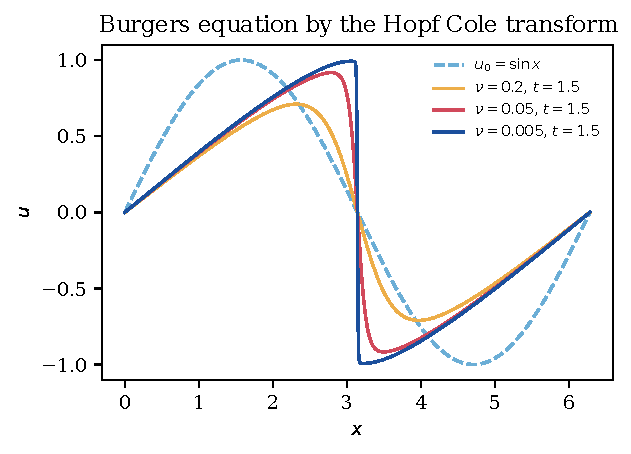
\includegraphics[width=0.92\textwidth]{burgers}
\caption{Solutions of the Burgers equation at $t=1.5$ for $\nu=0.2$, $0.05$ and $0.005$, computed by quadrature of the Hopf Cole formula from the initial condition $u_0=\sin x$, which is also drawn. The shock at $x=\pi$ forms in the inviscid limit.}
\label{fig:burgers}
\end{figure}

Burgers turbulence, the statistical theory of Burgers equation with random initial data or forcing, was developed by Sinai~\cite{sinai1992}, by E, Khanin, Mazel and Sinai~\cite{ekms2000}, and by others. For forcing that is periodic in space and white in time the inviscid equation has a unique invariant measure~\cite{ekms2000}, described through one sided minimizers of the action, and the structure functions scale as $S_p(\ell)\propto\ell$ for $p\geq1$ as $\ell\to0$~\cite{evandeneijnden2000}, a pure bifractal intermittency caused by the shocks. The exponents are therefore known exactly, which makes the model a test case for statistical methods that estimate scaling exponents from data.

\section{Inferring the dissipation rate}\label{sec:infer_dissipation}

The four fifths law gives a moment equation for $\varepsilon$, but in practice the inertial range is short and the third order structure function is noisy. A Bayesian model combines all scales. Let $\delta u_\parallel(\ell_j)$ be measured longitudinal increments at separations $\ell_1<\dots<\ell_J$. Conditionally on a local dissipation $\varepsilon_\ell$ at scale $\ell$, the K62 hypothesis gives increments of the form $\delta u\approx(\varepsilon_\ell\ell)^{1/3}Z$ with $Z$ a skewed variable independent of $\varepsilon_\ell$ and $\E Z^3 = -\frac45$, and $\log\varepsilon_\ell$ Gaussian with mean $\log\varepsilon-\frac{\mu}{2}\log(L/\ell)$ and variance $\mu\log(L/\ell)$, where $\mu$ is the intermittency coefficient. The mean and variance give $\E\varepsilon_\ell = \varepsilon$, so that $\E(\delta u)^3 = \ell\,\E\varepsilon_\ell\,\E Z^3 = -\frac45\varepsilon\ell$, which is the four fifths law. The model is a scale mixture in the sense of Chapter~\ref{ch:mixtures}, with lognormal mixing, and data augmentation over the latent $\varepsilon_\ell$ gives a posterior for $(\varepsilon,\mu,L)$ that can be sampled by Markov chain Monte Carlo. For a general law of $Z$ the lognormal mixing is not conjugate and the sampler needs Metropolis steps. We have not carried out the computation. The posterior of $\mu$ would be the statistical quantity behind the debate over the departure of structure function exponents from $p/3$, and the posterior of $\varepsilon$ given finite resolution data would quantify how sharply the anomalous dissipation hypothesis can be tested.

\section*{Exercises}
\begin{enumerate}
\item Verify that the Hopf Cole substitution transforms the Burgers equation into the heat equation.
\item Write the stationary elliptic system satisfied by a Leray self similar profile $U$.
\item Derive Fieller's interval for the ratio of two jointly Gaussian quantities with known covariance.
\item Using the scaling $u_\lambda(t,x) = \lambda^{2\alpha-1}u(\lambda^{2\alpha}t,\lambda x)$, show that the energy is critical for the hypodissipative equations in three dimensions exactly when $\alpha = 5/4$.
\item For the inviscid Burgers equation with $u_0 = \sin x$, show that the shock forms at time one.
\end{enumerate}


\section*{Notes}

Robinson, Rodrigo and Sadowski~\cite{robinson2016} treat the three dimensional regularity problem in detail. Frisch's \emph{Turbulence: The Legacy of A.\,N.~Kolmogorov}~\cite{frisch1995} is the standard account of K41, K62 and multifractals. De Lellis and Sz\'ekelyhidi~\cite{delellisszekelyhidi2017} survey convex integration and Onsager's conjecture, and Eyink and Sreenivasan~\cite{eyinksreenivasan2006} review Onsager's work on turbulence, published and unpublished.


\part{Generative Computation on the Solution Manifold}\label{part:manifold}
\chapter{The Inverse Problem on the Solution Manifold}
\label{ch:manifold}

\section{What the posterior is, and how to compute it}\label{m:sec:intro}

An experimenter observes a fluid, a temperature field, or a wave at $N$ scattered points in space and time, each measurement corrupted by noise, and believes the field obeys a known evolution equation. They want three things: the state of the system, its uncertainty, and its future. In the Bayesian formulation this is the regression model
\begin{equation}\label{m:eq:introm}
Y_i=u_\theta(t_i,x_i)+\varepsilon_i,\qquad i=1,\dots,N,
\end{equation}
in which $u_\theta$ is the solution of the equation with initial condition $\theta$ and the prior is placed on $\theta$. Nickl and coauthors have developed its statistical theory for nonlinear parabolic equations~\cite{nickltiti2024,nicklbvm2024,konennickl2026,nickl2025}. With a Gaussian process prior on $\theta$ and observations beginning at time zero, the posterior on $\theta$ is asymptotically Gaussian in a weak topology, the posterior on the state at any later time is asymptotically Gaussian in supremum norm at the parametric rate $1/\sqrt N$, credible bands have exact asymptotic coverage, and the posterior mean trajectory attains the local asymptotic minimax bound. Within its scope this is a complete answer to what the posterior is and what it is worth.

None of this answers how the posterior is to be obtained at the sample sizes one has, or what should be done when its hypotheses fail. Those are the questions that Part~\ref{part:manifold}, of which this chapter is the first, takes up. The tool is generative Bayesian computation (GBC)~\cite{polsonsokolov2025,polsonsokolov2026b}, developed in general in Chapter~\ref{ch:gbc}, which replaces sampling by a learned inverse map; the aim is to improve the framework's computational side while inheriting every guarantee it provides, and to say precisely where its guarantees stop. Chapter~\ref{ch:adjoint} constructs the summary statistic on which the generator conditions and says when it is sufficient, Chapter~\ref{ch:generators} shows when a generator trained on it inherits the guarantees of the framework and how to train it, and Chapter~\ref{ch:examples} works through the heat, Navier Stokes and Schr\"odinger equations and reports the experiments. This chapter states what they share, in the notation of this part: the framework, which Chapter~\ref{ch:nsinference} summarizes, the solution manifold, and the algorithm. Apart from the quoted results of the framework, this part is our own work~\cite{polsonsokolov2026manifold} and, to our knowledge, new; Section~\ref{m:sec:contrib} separates what is taken from what is added and what is conditional.

\subsubsection{The solution manifold} The lever is an idea the framework uses without naming. Because the prior is on the initial condition and the field is obtained by solving forward, every posterior draw satisfies the equation: the posterior lives on the solution manifold $\mathcal M=\{u_\theta\}$, the Gaussian limit of the theory is a Gaussian on its tangent space, and the chart $\theta\mapsto u_\theta(t)$ contracts under dissipation, damping mode $j$ by $e^{-\nu\lambda_jt}$. That contraction is quantifiable: for the heat equation at $N=2000$, against a space time Gaussian process prior of the same regularity that predicts the same variance for every observation, the manifold posterior has $20$ effective parameters where the unconstrained one has $116$, and it is $1.4$ times tighter at the initial time and $6.1$ times tighter at the end of the window (Section~\ref{m:sec:manifold}, Table~\ref{m:tab:gain}). Generative Bayesian computation computes on $\mathcal M$ directly (Algorithm~\ref{m:alg:gbc}).

\subsubsection{What the generator conditions on} The summary is the other half of the construction, and it too comes from the equation. For a linear dissipative equation the correct summary is the data themselves, run backward in time through the adjoint equation as point sources at the observation locations and read off at $t=0$; it is exactly sufficient. For a nonlinear equation there is no finite dimensional sufficient statistic, but the Bernstein von Mises theorem makes the posterior asymptotically Gaussian with data independent covariance, and a one step efficient score statistic, one forward and one adjoint solve at a preliminary estimate, is $\sqrt N$ equivalent to Nickl's centering. Under the uniform Bernstein von Mises statement of Assumption~\ref{m:ass:U} the posterior mean and this statistic are sufficient for the whole law at the $\sqrt N$ scale (Theorem~\ref{m:thm:jwbvm}).

\subsubsection{Where the asymptotics stop} The affine structure that the Bernstein von Mises theorem supplies holds on a shrinking neighborhood of the truth, and a generator trained on the prior does not see it: in the nonlinear experiment of Section~\ref{m:sec:expns}, such a generator stays about one posterior standard deviation from the Metropolis reference at every budget tried. Section~\ref{m:sec:loc} gives the theory of the remedy, which is to train where the affine structure holds.

\subsubsection{Examples} Three equations carry this part, and they differ in what the dynamics forget. The first is the heat equation, where every object is explicit and the asymptotic formulas can be checked against the exact posterior at finite $N$ (Section~\ref{m:sec:heat}). The second is two dimensional Navier Stokes about the Taylor Green vortex~\cite{taylorgreen1937} (Section~\ref{m:sec:ns}). The third is the Schr\"odinger equations (Section~\ref{m:sec:nondiss}), which show what dissipation was doing.

\subsubsection{Notation} $\Omega=[0,1]^d$ is the $d$ dimensional torus (periodic), $(e_j)$ the Laplace eigenbasis with $-\Delta e_j=\lambda_je_j$, $\lambda_j=4\pi^2|k_j|^2\asymp j^{2/d}$, and $H^a$ the periodic Sobolev spaces with $\norm{h}_{H^a}^2=\sum_j(1+\lambda_j)^a\langle h,e_j\rangle^2$; $H^{-a}$ is the dual. On the mean zero subspaces $H^a_0=\{h\in H^a:\langle h,1\rangle=0\}$, where $\lambda_j\ge\lambda_1>0$, the weights $\lambda_j^a$ give an equivalent norm, which differs from this one by at most the factor $(1+1/\lambda_1)^{|a|/2}$~\cite{nicklbvm2024}; where a norm is written out below as a weighted sum, it uses the weights shown, and no convergence statement depends on the choice. This is the convention of the general theory and of the heat and Schr\"odinger equations; the Taylor Green vortex and the Navier Stokes experiment are written on the $2\pi$ periodic torus, where $\lambda_k=|k|^2$, and Section~\ref{m:sec:ns} gives the conversion. $\Gcal(\theta)=u_\theta$ is the forward map, $\I_\theta=D\Gcal_\theta$ its linearization, and $\I_\theta^*$ the adjoint with respect to $L^2(\Omega)$ and $L^2([0,T]\times\Omega)$ with unnormalized Lebesgue measure. Because the design in \eqref{m:eq:model} is uniform on $\mathcal X=[0,T]\times\Omega$, whose measure is $T$, the Fisher information for $N$ observations in direction $h$ is $\tfrac NT\langle h,\I^*_\theta\I_\theta h\rangle$ and every asymptotic covariance below carries the factor $T$: the Bernstein von Mises limit is $N(0,T(\I^*\I)^{-1})$, which for the heat and Stokes equations, where $\I^*\I$ is diagonal in $(e_j)$, has diagonal $1/\iota_j$, with $\iota_j$ the per mode information of \eqref{m:eq:gram}. Setting $T=1$, as all numerical examples do, collapses the distinction. $\Wone_{1,B}$ is the Wasserstein distance of order one on a Banach space $B$, and $\Ccal=C([t_{\min},t_{\max}],C(\Omega))$, or $C([t_{\min},t_{\max}],C(\Omega)^2)$ for a vector field, is the trajectory space with the supremum norm, so $\Wone_{1,\Ccal}$ is that distance on it. $\Law$, $E$, $\Var$ under the posterior are conditional on the data $Z^{(N)}$; $P^\N_{\theta_0}$ is the law of the data under the truth. $a\lesssim b$ means $a\le Cb$ with $C$ independent of $N$. Observation noise is written $\varepsilon$, and the discrepancies and contraction rates of Chapters~\ref{ch:adjoint} and~\ref{ch:generators} are written $\epsilon$.

\section[\texorpdfstring{The Nickl framework for nonlinear Bayesian\newline estimation}{The Nickl framework for nonlinear Bayesian estimation}]{The Nickl framework for nonlinear Bayesian estimation}\label{m:sec:papers}

The framework this part builds on is a sequence of papers by Nickl and coauthors that settle, for nonlinear parabolic equations, the questions a Bayesian statistician asks of data assimilation. The standard reference for the theory these papers sit in is Nickl~\cite{nickl2023book}.

\subsection{Nickl (2024): the template}

The setting is random design regression on the space time cylinder $\mathcal X=[0,T]\times\Omega$, $\Omega=[0,1]^d$ the torus,
\begin{equation}\label{m:eq:model}
Y_i=\Gcal(\theta)(X_i)+\varepsilon_i,\qquad X_i=(t_i,x_i)\sim\mathrm{Unif}(\mathcal X),\qquad\varepsilon_i\sim N(0,I_W),
\end{equation}
where $\Gcal(\theta)=u_\theta$ is the solution map of $\partial_tu=\Delta u+F(u)$, $u(0)=\theta$. The prior is a rescaled Gaussian series in the Laplace eigenbasis $(e_j)$ with eigenvalues $\lambda_j\asymp j^{2/d}$,
\begin{equation}\label{m:eq:prior}
\theta=\frac{1}{\sqrt N\delta_N}\theta',\qquad\theta'=\sum_j\lambda_j^{-\gamma/2}g_je_j,\qquad\delta_N=N^{-\gamma/(2\gamma+d)},
\end{equation}
with RKHS $H_0^\gamma$ (Condition 1 there). The factor $1/(\sqrt N\delta_N)$ multiplies the squared RKHS norm by $N\delta_N^2$, so that prior and likelihood are on the same scale at the rate $\delta_N$; Nickl uses it to control the nonlinearity, and for the heat and Stokes equations a fixed prior has the same Bernstein von Mises limit (Proposition~\ref{m:prop:regfixed}). Readers outside this literature may read \eqref{m:eq:prior} as the series prior of a $\gamma$ smooth function, shrunk to the statistical resolution of $N$ observations. Condition 2 lists what the forward map must satisfy on Sobolev balls: (A) uniform $L^\infty$ bounds; (B) $L^2$ Lipschitz continuity; (C) a linearization $\I_{\theta_0}=D\Gcal_{\theta_0}$ with quadratic remainder; (D) $L^\infty$ mapping properties from $H^\zeta$, $\zeta>d/2$; (E) the stability estimate $\norm{\Gcal(\theta)-\Gcal(\theta_0)}_{L^2(\mathcal X)}\ge c\norm{\theta-\theta_0}_{H^{-1}}$; (F) invertibility of the information operator: $\Delta\I^*_{\theta_0}\I_{\theta_0}$ is a homeomorphism of $H^\eta_0$ for $\eta\ge\eta_0$.

\begin{theorem}[Nickl~\cite{nicklbvm2024}, Theorem 2]\label{m:thm:nickl2}
Under Conditions 1 and 2 with integer $\gamma>\max(3\zeta+3d/2+2,\eta_0)$ and $k>\max(\zeta+5d/2,\eta_0)$, with $\tilde\theta_N=E^\Pi[\theta\mid Z^{(N)}]$,
\begin{gather*}
\Wone_1\big(\Law(\sqrt N(\theta-\tilde\theta_N)\mid Z^{(N)}),\,\Ncal_{\theta_0}\big)\to^{P^{\N}_{\theta_0}}0,\\
\sqrt N(\tilde\theta_N-\theta_0)\to^d\Ncal_{\theta_0}\ \text{in }H^{-k-2},
\end{gather*}
where $\Wone_1$ is the Wasserstein distance of order one on $H^{-k-2}(\Omega)$ and $\Ncal_{\theta_0}=N(0,T(\I_{\theta_0}^*\I_{\theta_0})^{-1})$ is tight on $H^{-a}$ for $a>1+d/2$.
\end{theorem}

\begin{theorem}[Nickl~\cite{nicklbvm2024}, Theorem 1]\label{m:thm:nickl1}
For $\partial_tu-\Delta u=f(u)$, $f\in C_c^\infty(\R)$, $d\le3$, integer $\gamma>2+3d$, $\theta_0$ smooth, any $0<t_{\min}<t_{\max}<\infty$, and $\Ccal=C([t_{\min},t_{\max}],C(\Omega))$,
\begin{gather*}
\Wone_1\big(\Law(\sqrt N(u_\theta-u_{\tilde\theta_N})\mid Z^{(N)}),\,\mu\big)\to^{P^\N_{\theta_0}}0,\\
\sqrt N(u_{\tilde\theta_N}-u_{\theta_0})\to^d_\Ccal\mu,
\end{gather*}
where $\mu$ is the law in $\Ccal$ of the solution $U$ of $\partial_tU-\Delta U-f'(u_{\theta_0})U=0$, $U(0)=\vartheta\sim\Ncal_{\theta_0}$.
\end{theorem}

Two features of the proofs are used below. Theorem~\ref{m:thm:nickl1} follows from Theorem~\ref{m:thm:nickl2} by a two term decomposition: a linearization error controlled by concentration of the posterior on a localization set $\bar\Theta_N$, and a term bounded by $\Lip(\I_{\theta_0})$ times the Wasserstein distance in Theorem~\ref{m:thm:nickl2}, using that parabolic smoothing makes $\I_{\theta_0}$ continuous from $H^{-k-2}$ into $\Ccal$. And Theorem~\ref{m:thm:nickl2} is first proved with the centering
\begin{equation}\label{m:eq:thetahat}
\begin{aligned}
\hat\theta_N&=\sum_{j\ge1}\hat\Psi_{N,j}e_j,\\
\hat\Psi_{N,j}&=\langle e_j,\theta_0\rangle+\frac1N\sum_{i=1}^N\big\langle\I_{\theta_0}p_N(\bar e_j)(X_i),\varepsilon_i\big\rangle_W,\\
\bar e_j&=T(\I_{\theta_0}^*\I_{\theta_0})^{-1}e_j,
\end{aligned}
\end{equation}
with $p_N$ the projection onto the first $J_N\asymp N\delta_N^2$ modes, and then transferred to $\tilde\theta_N$. Equation \eqref{m:eq:thetahat} is the efficient influence function of the model and is the starting point of Section~\ref{m:sec:suff}.

Nickl outlines how Theorem~\ref{m:thm:nickl1} gives credible bands of exact asymptotic coverage and refers for the argument to Corollary~1.3 of Konen and Nickl~\cite{konennickl2026}. That argument uses that the limit law $\mu$ is nondegenerate, which Konen and Nickl prove for Navier Stokes. For the reaction diffusion class of Theorem~\ref{m:thm:nickl1} we prove it here.

\begin{lemma}[The limit law is nondegenerate]\label{m:lem:nondeg}
In the setting of Theorem~\ref{m:thm:nickl1}, the reproducing kernel Hilbert space (RKHS) of $\mu$ is a nontrivial linear subspace of $\Ccal$, and $r\mapsto\mu(\norm U_\Ccal\le r)$ is continuous and strictly increasing on $[0,\infty)$.
\end{lemma}

\begin{proof}
Let $V=f'(u_{\theta_0})$, so that $|V|\le K_f:=\sup|f'|<\infty$, and let $U_1=\I_{\theta_0}e_1$ be the solution of $\partial_tU_1=\Delta U_1+VU_1$, $U_1(0)=e_1$, which is smooth because $e_1$ is and $V$ is smooth in $x$ and continuously differentiable in $t$~\cite{nicklbvm2024}. First, $e_1$ lies in the RKHS of $\Ncal_{\theta_0}=N(0,T(\I^*_{\theta_0}\I_{\theta_0})^{-1})$: by Condition 2F, which Nickl verifies for this class, $\psi=T^{-1}\I^*_{\theta_0}\I_{\theta_0}e_1$ is smooth, and the covariance maps $\psi$ to $e_1$ (Section~2.2.2 of Nickl's paper~\cite{nicklbvm2024}). Second, $\I_{\theta_0}$ is continuous from $H^{-k-2}$ into $\Ccal$ and $\mu$ is the image of $\Ncal_{\theta_0}$ under it, so the RKHS of $\mu$ is the image of the RKHS of $\Ncal_{\theta_0}$ (Exercise~2.6.5 of Gin\'e and Nickl~\cite{ginenickl2016}, as Konen and Nickl use it) and contains $U_1$. Third, $U_1$ does not vanish. With $A=-\Delta$, the inner product of $L^2(\Omega)$, $q=\langle AU_1,U_1\rangle/\norm{U_1}^2$ and $w=(A-q)U_1$, as long as $U_1(t)\ne0$,
\[
\begin{aligned}
q'&=2\norm{U_1}^{-2}\big(-\norm w^2+\langle w,VU_1\rangle\big)\le K_f^2/2,\\
\big(\log\norm{U_1}^2\big)'&=-2q+2\norm{U_1}^{-2}\langle VU_1,U_1\rangle\ge-2q-2K_f,
\end{aligned}
\]
the first because $-x^2+xy\le y^2/4$ and $\norm{VU_1}\le K_f\norm{U_1}$. Since $q(0)=\lambda_1$, it follows that $q(t)\le\lambda_1+K_f^2t/2$ and
\[
\norm{U_1(t)}^2\ge\exp\big(-2(\lambda_1+K_f)t-K_f^2t^2/2\big)
\]
on the largest interval $[0,t_*)$ on which $U_1$ does not vanish, hence at $t_*$ by continuity, so that $t_*=\infty$ and $\norm{U_1}_\Ccal\ge\norm{U_1(t_{\min})}_{L^2(\Omega)}>0$. The RKHS of $\mu$ is a linear space that contains $U_1\ne0$, so it contains elements of every norm. The rest is the argument of Konen and Nickl for Navier Stokes (Section~2.6 of their paper~\cite{konennickl2026}): the distribution function of $\norm U_\Ccal$ is continuous by Exercise~2.4.4 of Gin\'e and Nickl, and it is strictly increasing because every shell $\{r<\norm u_\Ccal<s\}$ contains a ball of radius $(s-r)/3$ centered at an element of the RKHS of $\mu$, and such a ball has positive $\mu$ measure by Theorem~2.4.5 and Corollary~2.6.18 of Gin\'e and Nickl.
\end{proof}

\subsection{Navier Stokes, the barrier, and McKean Vlasov}

For the periodic two dimensional Navier Stokes system $du/dt+\nu Au+B[u,u]=f$, $u(0)=\theta$, with Stokes operator $A=-\Delta$ on divergence free mean zero fields $\Hds{}$, $B[u,v]=P[(u\cdot\nabla)v]$, prior $N(0,\rho_N^2A^{-\alpha})$, $\alpha>12$, and observations on $[0,T]\times\T^2$, Theorems~\ref{m:thm:nickl2} and~\ref{m:thm:nickl1} hold with $\Ncal_{\theta_0}=N(0,T(\I^*_{\theta_0}\I_{\theta_0})^{-1})$ tight on $\Hds{-\beta}$, $\beta>2$, RKHS $\Hds{-1}$, and $\Ccal=C([t_{\min},t_{\max}],C(\Omega)^2)$~\cite{konennickl2026}. The two new ingredients are a Lipschitz stability estimate at $t=0$ without symmetry of the linearized operator, and the Fredholm decomposition
\begin{equation}\label{m:eq:fredholm}
\begin{gathered}
\I_\theta^*\I_\theta=\Lcal^*\Lcal+\Kcal,\qquad \Delta\Lcal^*\Lcal=\frac1{2\nu}\big(S_{2T}-\Id\big),\\
\Kcal\ \text{compact }\Hds{a}\to\Hds{a+2},
\end{gathered}
\end{equation}
where $\Lcal$ is the Stokes (heat) solution operator with semigroup $S_t=e^{\nu t\Delta}$. The same paper adds exact asymptotic coverage of credible bands (Corollary 1.3 there) and, via Konen~\cite{konen2026}, a local asymptotic minimax theorem attained by the posterior mean trajectory (Theorem 1.2 there). Mode by mode, \eqref{m:eq:fredholm} reads
\begin{equation}\label{m:eq:modeinfo}
\big\langle e_j,\Lcal^*\Lcal\,e_j\big\rangle=\int_0^Te^{-2\nu\lambda_jt}\,dt=\frac{1-e^{-2\nu\lambda_jT}}{2\nu\lambda_j},
\end{equation}

Nickl and Titi~\cite{nickltiti2024} prove consistency for the same Navier Stokes posterior with, in general, inverse logarithmic contraction rates, and a matching lower bound when observations are supported on $[T_0,T]$, $T_0>0$. They also describe conditions on the initial condition under which faster rates are possible, and Konen and Nickl~\cite{konennickl2026attractor} prove, for initial conditions on the global attractor of a two dimensional periodic reaction diffusion system, an $L^2$ Lipschitz stability estimate for $\theta\mapsto u_\theta(t)$ at any fixed $t>0$ and near parametric rates for the initial condition and the states. Nickl, Pavliotis and Ray~\cite{nickl2025} treat the McKean Vlasov equation, inferring the interaction potential from space time density data; the forward model is the mean field limit of a particle system, which makes it the natural meeting point of GBC with the particle side of the sixth problem (Section~\ref{m:sec:hilbert}).

\subsection{What the framework establishes, and what it leaves open}\label{m:sec:gaps}

The framework establishes, for parabolic equations with a Gaussian series prior on the initial condition and observations from time zero: contraction at the nonparametric rate $\delta_N$~\cite{nickltiti2024,nicklbvm2024}; the weak topology Bernstein von Mises theorem (Theorem~\ref{m:thm:nickl2}); its lift to the supremum norm on forward trajectories through parabolic smoothing (Theorem~\ref{m:thm:nickl1}); and, proved by Konen and Nickl for Navier Stokes~\cite{konennickl2026}, exact asymptotic coverage of credible bands and local asymptotic minimax efficiency of the posterior mean trajectory, the first also for the reaction diffusion class (Lemma~\ref{m:lem:nondeg}). Nickl and Wang~\cite{nicklwang2024} add that localized Langevin sampling computes the posterior in time polynomial in $N$, the dimension, and the inverse accuracy, in a related steady state elliptic model; Section~\ref{sec:gradstab} obtains their gradient stability for the heat equation and, when time zero is observed, for the initial condition of two dimensional Navier Stokes, and verifying their remaining conditions for the initial condition of a nonlinear time evolution equation is open as far as we know. The framework leaves open, or does not address, seven things that this part takes up.

\begin{enumerate}
\item Computation by generation rather than sampling: whether a learned inverse map can reach the posterior at the $\sqrt N$ scale, and under what hypothesis (Section~\ref{m:sec:main}).
\item What the data must be reduced to: the framework proves the Bernstein von Mises theorem for the full data and never asks for a sufficient statistic (Section~\ref{m:sec:suff}).
\item Whether reducing to a sufficient statistic improves any bound, or merely preserves one (Section~\ref{m:sec:suffbounds}).
\item How a generator must be trained: the affine structure the theorem supplies is a statement on a shrinking neighborhood, and a training distribution that ignores this fails (Section~\ref{m:sec:loc}).
\item Finite $N$: the accuracy of the Gaussian limit at the sample sizes one has (Proposition~\ref{m:prop:gram}, and the numerical study of Polson and Sokolov~\cite{polsonsokolov2026}).
\item Nondissipative equations: the framework is parabolic throughout (Section~\ref{m:sec:nondiss}).
\item Model error and non Gaussian priors, which the framework excludes by assumption (Theorem~\ref{m:thm:PR} and Section~\ref{m:sec:open}). The framework also assumes Gaussian noise, and so does this part.
\end{enumerate}

\section{The solution manifold: solve for the initial condition, then simulate forward}\label{m:sec:manifold}

The framework of Section~\ref{m:sec:papers} constrains the initial condition, but the object it constrains is the trajectory. Every draw from the posterior is a solution of the equation, so the posterior lives on the set of space time fields the equation can produce, and that set is parameterized by $\theta$ alone.

\subsection{The manifold and its tangent space}

Let $\Theta$ be the parameter space of initial conditions and $\Gcal:\Theta\to C([0,T],L^2(\Omega))$ the solution map. The set
\begin{equation}\label{m:eq:manifold}
\mathcal M=\{u_\theta=\Gcal(\theta):\theta\in\Theta\}
\end{equation}
is the solution manifold: the space time fields that satisfy the PDE for some admissible initial datum. When $\Theta$ is the $D$ dimensional truncation of the Gaussian series prior, $\mathcal M$ is a $D$ dimensional embedded submanifold of the space of space time fields, with tangent space at $u_{\theta_0}$ equal to the range of the linearization $\I_{\theta_0}$. The Nickl framework parameterizes the unknown field by its initial condition and puts the prior on $\theta$; the posterior on the field is the push forward $\Gcal_\#\Pi(\cdot\mid Z^{(N)})$. Three consequences follow, none stated in the framework but all used by it.

\begin{proposition}[Posterior on the manifold]\label{m:prop:manifold}
\begin{enumerate}[label=(\roman*)]
\item Every draw from the posterior on the field satisfies the equation exactly: $\Gcal_\#\Pi(\cdot\mid Z^{(N)})$ is supported on $\mathcal M$ for every $N$, and so is every draw of the GBC posterior of Algorithm~\ref{m:alg:gbc}, since it is obtained by simulating forward.
\item The Gaussian limit $\mu$ of Theorem~\ref{m:thm:nickl1} is the law of $\I_{\theta_0}[\vartheta]$, $\vartheta\sim\Ncal_{\theta_0}$: a centered Gaussian measure supported on the tangent space $T_{u_{\theta_0}}\mathcal M$, with covariance the push forward of $T(\I^*_{\theta_0}\I_{\theta_0})^{-1}$ by $\I_{\theta_0}$.
\item Forward prediction beyond the observation window is the restriction of the same posterior to $t>T$; it requires no extrapolation model, and, when the data come from the model and the hypotheses of Theorem~\ref{m:thm:nickl1} or of its Navier Stokes counterpart hold, its uncertainty at the $\sqrt N$ scale is asymptotically that of the tangent space Gaussian propagated by the tangent equation, on any window $[t_{\min},t_{\max}]$, also one with $t_{\max}>T$.
\end{enumerate}
\end{proposition}

\begin{proof}
(i) is the definition of the push forward and of the forward simulation. (ii) is the statement of Theorem~\ref{m:thm:nickl1} read as a statement about where the limit lives. The first part of (iii) is that $u_\theta$ is defined on $[0,\infty)$ and the posterior on $\theta$ does not know where the observations stopped. The second is Theorem~\ref{m:thm:nickl1}, and its Navier Stokes counterpart~\cite{konennickl2026}, whose window $0<t_{\min}<t_{\max}<\infty$ is arbitrary and may extend beyond $T$; the limit $\mu$ there is the law of the solution of the tangent equation started from $\vartheta\sim\Ncal_{\theta_0}$, which is the Gaussian of (ii).
\end{proof}

None of this holds for a Gaussian process prior placed directly on the space time field: that posterior is supported on the whole function space, its draws do not satisfy the equation, it cannot predict beyond $T$ without an extrapolation assumption, and its effective dimension is that of a field rather than of an initial condition. This is what separates the construction here from the physics informed and PDE constrained Gaussian process literature, which places the prior on the field and then imposes the equation as a constraint or a penalty: Raissi, Perdikaris and Karniadakis~\cite{raissi2017} use the linearity of the operator to push a Gaussian process through it exactly, and Chen and coauthors~\cite{chen2021} solve and learn nonlinear equations by collocating a Gaussian process against the residual. Putting the prior on the initial condition and simulating forward makes the constraint free, since the parametrization cannot leave $\mathcal M$. Proposition~\ref{m:prop:gain} prices the difference in the one case where both posteriors are available in closed form, and the comparison it makes is against an \emph{unconstrained} field prior. A Gaussian process conditioned on a linear equation is supported on the same manifold~\cite{albertrath2020}, so against that competitor the gain of Table~\ref{m:tab:gain} is not available; what survives the comparison is that here the constraint extends past $T$ without an extrapolation assumption.

\subsection{The manifold gain, quantified}

\begin{proposition}[Manifold gain for the heat equation]\label{m:prop:gain}
Consider the heat equation on $\T^d$, let $\alpha>(d+1)/2$, and take the prior $\sigma_{0,j}^2=\rho^2(\lambda_j/\lambda_1)^{-\alpha}$ on the initial condition (constrained model), and, for comparison, a Gaussian process prior on the space time field $u(t,x)$ with Fourier variances $\rho^2((\lambda_k+\omega_m^2)/\lambda_1)^{-\alpha}$, $\omega_m=2\pi m/T$ (unconstrained model), so that the two priors have comparable regularity in $x$. With $N$ observations uniform on $[0,T]\times\T^d$, the Gram matrix of the design replaced by its limit, namely $\diag(\iota_j)$ by \eqref{m:eq:gram} in the constrained model and the identity in the unconstrained one, and noise variance $\varsigma^2$, which is the variance normalized to one in \eqref{m:eq:model} and is carried as a symbol here and in Sections~\ref{m:sec:suff} and~\ref{m:sec:jw} only to show where it enters:
\begin{enumerate}[label=(\roman*)]
\item the constrained posterior standard deviation of $u(t,x)$ is $\big(\sum_je^{-2\nu\lambda_jt}(N\iota_j/\varsigma^2+\sigma_{0,j}^{-2})^{-1}\big)^{1/2}$, decreasing in $t$, and the effective number of parameters is $J_{\rm eff}\asymp(N\rho^2/\nu T)^{d/(2\alpha+2)}$ (Theorem~\ref{m:thm:jeff});
\item the unconstrained posterior standard deviation is $\big(\sum_{k,m}(N/\varsigma^2+\sigma_{0,km}^{-2})^{-1}\big)^{1/2}$, independent of $(t,x)$, and its effective number of parameters is $\#\{(k,m):N\sigma^2_{0,km}\ge\varsigma^2\}\asymp N^{(d+1)/(2\alpha)}$;
\item the ratio of unconstrained to constrained standard deviation at time $t$ is at least $e^{\nu\lambda_1t}$ times its value at $t=0$, so it grows without bound as $t$ increases, at the rate at which the manifold contracts.
\end{enumerate}
\end{proposition}

\begin{proof}
(i) is \eqref{m:eq:linpost} pushed through the heat semigroup, with the Gram concentration \eqref{m:eq:gram}; the parameter count is Theorem~\ref{m:thm:jeff}(i). (ii) is the same computation in the orthonormal space time Fourier basis, where the design is asymptotically orthonormal in both variables; the count follows from $\#\{(k,m):\lambda_k+\omega_m^2\le\Lambda\}\asymp\Lambda^{(d+1)/2}$ with $\Lambda\asymp N^{1/\alpha}$. (iii) the standard deviation in (ii) does not depend on $t$, while by (i) the constrained variance at time $t$ is at most $e^{-2\nu\lambda_1t}$ times its value at $t=0$, because $\lambda_j\ge\lambda_1$ for every $j$.
\end{proof}

\begin{table}[tp]\centering\footnotesize\setlength{\tabcolsep}{3pt}
\caption{The manifold gain for the two dimensional heat equation, $N=2000$, $\nu=0.01$, $T=1$, $\alpha=3$, $\varsigma=1$, with matched priors: both use the spatial modes $k\in\Z^2$ with $0<\max(|k_1|,|k_2|)\le12$, so they exclude the spatial mean modes, and both give the signal $u(X_i)$ of an observation, with $X_i$ uniform on $[0,T]\times\Omega$, the prior standard deviation $1.75$, which takes $\rho=1$ in the constrained prior and $\rho=0.69$ in the unconstrained one, whose temporal frequencies are $|m|\le40$. The pointwise prior standard deviation is then $1.75$ at every $t$ in the unconstrained model and falls from $2.16$ at $t=0$ to $1.39$ at $t=1$ in the constrained one. Posterior standard deviation of $u(t,x)$ at a point.}\label{m:tab:gain}
\begin{tabular}{@{}>{\raggedright\arraybackslash}p{1.6in}>{\centering\arraybackslash}p{0.62in}ccccc@{}}
\toprule
& effective parameters & $t=0$ & $t=0.05$ & $t=0.2$ & $t=0.5$ & $t=1$\\
\midrule
constrained (on $\mathcal M$) & 20 & 0.227 & 0.194 & 0.137 & 0.085 & 0.051\\
unconstrained space time GP & 116 & 0.313 & 0.313 & 0.313 & 0.313 & 0.313\\
ratio & & 1.4 & 1.6 & 2.3 & 3.7 & 6.1\\
\bottomrule
\end{tabular}
\end{table}

Table~\ref{m:tab:gain} evaluates the proposition. How the priors are matched moves the ratio at the initial time but not its growth with $t$, a factor $4.4$ by $t=1$, since the unconstrained standard deviation does not depend on $t$. The unconstrained posterior is stationary in time because nothing in its prior distinguishes early from late; the constrained posterior improves with time because the manifold contracts under dissipation, so that a fixed uncertainty in the initial condition is damped by $e^{-\nu\lambda_jt}$ in every mode. This is the statistical content of parabolic smoothing, and it is the reason the Nickl framework obtains a $1/\sqrt N$ rate in supremum norm for the state at $t>0$ while the initial condition itself is recoverable only at the nonparametric rate.

\subsection{Three examples, and what the viewpoint changes}

\subsubsection{Heat and Stokes} $\mathcal M$ is the linear span $\{\sum_j\theta_je^{-\nu\lambda_jt}e_j\}$, a $D$ dimensional linear subspace of space time fields whose basis functions decay at mode dependent rates. The tangent space is $\mathcal M$ itself, the Gaussian limit is Gaussian on $\mathcal M$, and every Gaussian statement in Sections~\ref{m:sec:suff} to~\ref{m:sec:loc} is exact.

\subsubsection{Navier Stokes about the Taylor Green vortex} $\mathcal M$ is a nonlinear manifold, and the Taylor Green family $\{Ae^{-2\nu t}u_{\rm TG}(x):A\in\R\}$, written on the $2\pi$ periodic torus where $\lambda_k=|k|^2$ as in Section~\ref{m:sec:ns}, is a one dimensional submanifold along which the equation is exactly linear, because the nonlinear term is a gradient. Off that curve the tangent space at $u_{\rm TG}$ is spanned by solutions of the linearized equation with the nearest neighbor Fourier coupling \eqref{m:eq:tgcoupling}, which is where it departs from the tangent space of the Stokes flow, and the compact perturbation $\Kcal$ of the information operator measures how far the metric that the data induce on $\mathcal M$ at $u_{\rm TG}$, which is $\I^*\I$, is from the Stokes metric $\Lcal^*\Lcal$ of the flat case.

\subsubsection{Schr\"odinger} For the linear equation $\mathcal M$ is the orbit $\{e^{it\Delta}\theta\}$ of the unitary group: a manifold isometric to the space of initial conditions at every time, with no contraction. The manifold constraint still removes the space time degrees of freedom of an unconstrained model, but dissipation contributes nothing, so the gain of Proposition~\ref{m:prop:gain}(iii) is constant in $t$ rather than growing, and there is no supremum norm theorem because the chart does not smooth (Section~\ref{m:sec:nondiss}). For the cubic nonlinear Schr\"odinger equation (NLS) about a plane wave the metric that the data induce on the manifold departs from the flat $T\cdot\Id$ through the conjugation term of the linearized equation alone, and the Bogoliubov blocks of Proposition~\ref{m:prop:bog} give it mode by mode: a bounded perturbation in the defocusing case, and in the focusing band an exponential growth along one direction of each unstable block.

\subsubsection{What the viewpoint changes in the computation} Everything that follows comes from computing on $\mathcal M$ rather than in the ambient space. The sufficient statistic of Section~\ref{m:sec:suff} is the projection of the data onto the tangent space of $\mathcal M$, computed by the adjoint equation. The supremum norm part of the transfer theorem of Section~\ref{m:sec:main} holds because the forward simulation in the last step of Algorithm~\ref{m:alg:gbc} is the chart $\theta\mapsto u_\theta$, whose linearization is Lipschitz from $H^{-k-2}$ into the trajectory space by parabolic smoothing (Section~\ref{m:sec:papers}). The effective dimension of Theorem~\ref{m:thm:jeff} is the dimension of the part of $\mathcal M$ that the data resolve. And the localization of Section~\ref{m:sec:loc} is the statement that the generator should be trained where the manifold is flat, at the scale on which the framework's Gaussian limit lives. The sequential methods of Section~\ref{m:sec:connections} are the same idea in time: particle learning carries the coordinate $\theta$, the practical filter relinearizes the chart, and the Gibbs smoother of Carlin Polson Stoffer is what one does when model error takes the trajectory off $\mathcal M$.

\section{GBC for the initial condition problem}\label{m:sec:gbc}

Between the forward solves of Steps 1 and 4 of Algorithm~\ref{m:alg:gbc} sits a learning problem that is finite dimensional whatever $N$ is, because what the generator conditions on is a summary of the data and not the data.

Fix the model \eqref{m:eq:model} to \eqref{m:eq:prior} and a summary map $S_N:(\R^W\times\mathcal X)^N\to\R^{p_N}$. Let $U$ be a base random variable independent of everything.

\begin{algorithm}[GBC: solve for the initial condition, simulate forward]\label{m:alg:gbc}\leavevmode
\begin{enumerate}[nosep]
\item Simulate $M$ training pairs: $\theta^{(m)}\sim\Pi$, then $Z^{(m)}$ from \eqref{m:eq:model} with $\Gcal(\theta^{(m)})$ computed by a forward solve. Compute $S^{(m)}=S_N(Z^{(m)})$.
\item Train a conditional generator $\widehat G:\R^{p_N}\times\R^q\to L^2_0(\Omega)$ on $\{(S^{(m)},\theta^{(m)})\}$ so that $\Law(\widehat G(s,U))$ approximates $\Law(\theta\mid S_N(Z)=s)$. In coefficient form, $\widehat G(s,U)=\sum_j\widehat Q_j(U_j\mid s)e_j$ with $\widehat Q_j(\cdot\mid s)$ a learned conditional quantile function.
\item Define the GBC posterior $\Pihat:=\Law\big(\widehat G(S_N(Z^{(N)}),U)\big)$ conditional on the observed $Z^{(N)}$, and its mean $\hat\theta_N^{\rm G}$.
\item Simulate forward: for $\theta\sim\Pihat$, solve the PDE to obtain $u_\theta$; report $\Law(u_\theta(t)\mid Z^{(N)})$, functionals $\Phi(u_\theta)$, and credible bands.
\end{enumerate}
\end{algorithm}

Step 2 writes the generator in coefficient form, with one learned quantile function for each mode. The generator of Definition~\ref{m:def:gen} instead mixes the coordinates of the base noise through a full matrix, so it has this form only when that matrix is diagonal; the first of the four points in that definition explains why nothing downstream depends on the difference.

Three sample sizes appear and do different work. $N$ is the number of observations, and is the only one the asymptotics of Sections~\ref{m:sec:jw} to~\ref{m:sec:main} take to infinity. $M$ is the simulation budget, chosen by the user, and it is the quantity the generator theorems bound (Theorems~\ref{m:thm:qnnA} and~\ref{m:thm:raw}). The number of draws from $\Pihat$ in Steps 3 and 4 carries no statistical content, since $\Pihat$ is available as a map and can be sampled to any accuracy for the price of forward passes.

Steps 1 and 2 never see $Z^{(N)}$. They can be run before the data exist, and their cost, $M$ forward solves and one training run, is paid once; a new data set then costs one evaluation of $S_N$, one forward pass of $\widehat G$ per draw, and whatever forward solves are asked of Step 4. That is what amortization means here, and it is a claim about cost and not about accuracy.

Step 1 already constrains the summary map. It is applied to simulated data, so it must be a statistic: a function of $Z$ alone, with no dependence on the $\theta$ that produced it. This is why the one step summary of Section~\ref{m:sec:suff} is centered at a preliminary estimate computed from the data rather than at the truth, and why that estimate is cross fitted.

Write $\PiN=\Pi(\cdot\mid Z^{(N)})$ for the exact posterior and $\Pi(\cdot\mid S_N)$ for the posterior given the summary alone. Two discrepancies arise: $\Pi(\cdot\mid S_N)$ versus $\PiN$, which is sufficiency and the subject of Sections~\ref{m:sec:suff} and~\ref{m:sec:jw}, and $\Pihat$ versus $\Pi(\cdot\mid S_N)$, which is generator fit and enters the transfer theorem of Section~\ref{m:sec:main} through one accuracy assumption.

\section{What is taken, what is added, and what is conditional}\label{m:sec:contrib}

The results of Nickl~\cite{nicklbvm2024} and Konen and Nickl~\cite{konennickl2026} are used as black boxes and are not reproved. We take from them the model \eqref{m:eq:model} with the prior \eqref{m:eq:prior}, Conditions 2A to 2F on the forward map, Theorems~\ref{m:thm:nickl2} and~\ref{m:thm:nickl1}, the centering \eqref{m:eq:thetahat}, the Fredholm decomposition \eqref{m:eq:fredholm}, the exact coverage corollary and the local asymptotic minimax theorem, and the inverse logarithmic barrier of Nickl and Titi~\cite{nickltiti2024}. What follows is new relative to that framework, grouped by kind and in the order of the chapters that prove it.

\subsubsection{The sufficient statistic (Section~\ref{m:sec:suff})} For a linear evolution the adjoint equation driven by the data is exactly sufficient for the initial state, and the GBC quantile map is exactly affine with an explicit scale (Lemma~\ref{m:lem:adjoint}, Proposition~\ref{m:prop:linsuff}). For a nonlinear evolution the one step efficient score statistic in $J_N\asymp N\delta_N^2$ modes is $\sqrt N$ equivalent to Nickl's centering, hence a computable center for the Gaussian limit of the posterior (Definition~\ref{m:def:summary}, Proposition~\ref{m:prop:suff}), and it is asymptotically sufficient for the whole law under Assumption~\ref{m:ass:U} (Theorem~\ref{m:thm:jwbvm}); in the linear model its regularized form \eqref{m:eq:regsummary} is exactly the posterior mean, whatever the linearization point (Lemma~\ref{m:lem:exact}), and for the heat and Stokes equations that form remains $\sqrt N$ equivalent to Nickl's centering when $J_N$ modes are retained under the rescaled prior (Proposition~\ref{m:prop:regheat}). The same statistic then does three further things. It is recursively updatable in the linear case, so particle learning for the initial condition is exact without weight degeneracy (Proposition~\ref{m:prop:storvik}). It identifies the Bernstein von Mises covariance as a change in expected utility in the sense of Polson and Roberts~\cite{polsonroberts1993}, exactly in the linear Gaussian models of the heat and Stokes equations and, for a nonlinear forward map in the setting of Theorem~\ref{m:thm:nickl2} and a fixed number of modes, through the realized information gain of the posterior at the truth, whereas the expected gain is bounded by the information near the center of the prior (Corollary~\ref{m:cor:prreal}, Propositions~\ref{m:prop:prvt} and~\ref{m:prop:prrd}, and Remark~\ref{m:rem:prscope}), and separates the noise level from the initial condition by a quadratic variation argument set in the diffusion framework of Polson and Roberts~\cite{polsonroberts1994} (Propositions~\ref{m:prop:pr} and~\ref{m:prop:qv}). And it is what the summary selection literature selects: under Assumption~\ref{m:ass:U} it attains, asymptotically, the optimum of the four approximate Bayesian computation (ABC) criteria, of the $L^2$ Bayes risk for the exact posteriors under the moment bound~\eqref{m:eq:momentbound} and of the other three in the $J_N$ mode Gaussian projection, which is the limit for heat and Stokes; in the linear case the statistic is the partial least squares (PLS) projection; and in general it has the structure of deep PLS, introduced by Polson, Sokolov and Xu~\cite{polsonsokolovxu2021} and applied to instrumental variable regression by Nareklishvili, Polson and Sokolov~\cite{nareklishvili2023} (Propositions~\ref{m:prop:abcopt}, \ref{m:prop:pls} and~\ref{m:prop:dpls}).

\subsubsection{Sufficiency theorems and bounds (Sections~\ref{m:sec:jw} to~\ref{m:sec:suffbounds})} The posterior mean summary is first moment exact at every $N$ and, under the uniform Bernstein von Mises statement of Assumption~\ref{m:ass:U}, sufficient for the whole law at scale $\sqrt N$ (Theorems~\ref{m:thm:jw} and~\ref{m:thm:jwbvm}). When a summary is not sufficient the gap it leaves is bracketed below by its Rao Blackwell trace, with the operator norm correction of Theorem~\ref{m:thm:gap}, and above by $\sqrt{2\norm{V_S}_{op}\Delta I}$, both computable from the model (Theorem~\ref{m:thm:gap} in the linear Gaussian model, Proposition~\ref{m:prop:gapnl} beyond it, for a summary whose posterior, like the posterior given all of the data, is close at the $\sqrt N$ scale to that of one linear Gaussian model under the prior predictive law). Under the rescaled prior and clauses (U1) to (U3) of Assumption~\ref{m:ass:U} the posterior covariance of that model must be asymptotically the inverse information at the prior mean (Proposition~\ref{m:prop:gapreq}), and in a two coordinate nonlinear model the maximum likelihood coordinate is such a summary, while the first coordinate of the adjoint statistic at the prior mean is not, for any Gaussian model, once $\sqrt Ns_N^2\to\infty$ (Proposition~\ref{m:prop:gaptoy}). And the dimension the generator has to learn in is small under dissipation: the effective dimension of the sufficient statistic is of order $(N\rho^2/\nu T)^{d/(2\alpha+2)}$ as $N\to\infty$ at fixed $\nu T$, decreasing in viscosity (Theorem~\ref{m:thm:jeff}), against a simulation budget that is super exponential on the raw data for a generator required to be uniformly accurate and, conditionally on the hypotheses of Theorem~\ref{m:thm:qnnA}, linear in that effective dimension for the hybrid generator of Theorem~\ref{m:thm:jeff}(ii) trained on the statistic (Theorem~\ref{m:thm:raw}).

\subsubsection{Transfer, generators, and network priors (Sections~\ref{m:sec:main} to~\ref{m:sec:qnn})} Any $\sqrt N$ accurate, concentrating approximation to the posterior inherits the Gaussian limit, the supremum norm trajectory theorem, exact coverage and minimax efficiency (Theorem~\ref{m:thm:main}, whose proof isolates the properties of the posterior that Nickl's trajectory argument uses), and solving forward from the GBC draws agrees asymptotically with simulating the tangent equation from that limit (Corollary~\ref{m:cor:commute}). Which generators qualify is then settled in both directions: conditionally on Assumptions~\ref{m:ass:U} and~\ref{m:ass:u2p} and on a bound for the error of the summary, the identity skip Gaussian head quantile generator meets the accuracy hypothesis when $J_N/M_N\to0$ (Theorem~\ref{m:thm:qnnA}), and no generator required to be uniformly accurate over H\"older quantile maps can meet it with polynomially many simulations once $J_N\to\infty$ (Theorem~\ref{m:thm:qnnB}). Under the Polson Ro\v{c}kov\'a network prior, adaptive contraction transfers to the initial condition through the stability estimate (Theorem~\ref{m:thm:PR}) but the Bernstein von Mises step does not, because its Cameron Martin step has no network analog, and Section~\ref{m:sec:qnn} says what would be needed.

\subsubsection{Localized training (Section~\ref{m:sec:loc})} Training on a proposal of radius $c$ leaves a residual with mean $P\bar\theta$ and, in a basis that diagonalizes the prior and the Gram matrix together, variance $\Sigma_{N,j}(s_j+c^2p_j^2)$, so the mean has to be removed and the variance bias is of first order in the prior fraction (Theorem~\ref{m:thm:locbias}). The three error terms $\beta(c)^2+a_v/c^v+bc^4$ then fix, for the affine head, an optimal radius $c^\star\asymp(DN/Mc_3^2)^{1/6}$, which Figure~\ref{m:fig:radius} checks against measurement (Proposition~\ref{m:prop:radius}). What comes out is a design rule, Algorithm~\ref{m:alg:loc}: localize at $c\in[2,3]$, a calibration for the identity head and not a consequence of \eqref{m:eq:cstar} (Remark~\ref{m:rem:radiushead}), center and rescale the residuals, use the identity head, and do not importance weight.

\subsubsection{Examples and dispersive equations (Sections~\ref{m:sec:heat} to~\ref{m:sec:nondiss})} For the heat equation a matrix Bernstein bound controls the finite $N$ error of the Bernstein von Mises covariance, checked numerically against the exact posterior, with relative discrepancy below one percent in the calibrated runs (Proposition~\ref{m:prop:gram}, Figure~\ref{m:fig:heatgbc}, Table~\ref{m:tab:diag}), and Table~\ref{m:tab:iota} puts the Nickl Titi barrier in numbers. For Navier Stokes this part supplies the Stokes limit, the Taylor Green background, the explicit Fourier coupling \eqref{m:eq:tgcoupling} and the adjoint pipeline, together with the identity \eqref{m:eq:modeinfo} that reconciles Konen Nickl and Nickl Titi and that would give the curvature constant of Nickl and Wang if their remaining conditions were verified (Section~\ref{sec:gradstab}). Nothing in the framework treats dispersive equations, and two results say what changes there: for linear Schr\"odinger the information operator is exactly $T\cdot\Id$, also with a real potential (Section~\ref{m:sec:nondiss}), and for the free equation the transfer theorem holds in a reduced form, without a supremum norm statement (Proposition~\ref{m:prop:sch} and Corollary~\ref{m:cor:schtransfer}), while for cubic NLS about a plane wave the Bogoliubov information operator is a compact perturbation of $T\cdot\Id$ in the defocusing case and, in the focusing band, exponentially amplified along one direction of each unstable block (Proposition~\ref{m:prop:bog}). Condition 2E holds for its solution map by an energy estimate (Proposition~\ref{m:prop:nlsstab}), while Conditions 2C and 2D are not verified.

\subsubsection{Connections (Section~\ref{m:sec:connections})} Least squares Monte Carlo is the same construction, and its two limit convergence theory transfers (Proposition~\ref{m:prop:lsm}, Theorem~\ref{m:thm:lsmgbc}). Three shorter readings follow: the model error endpoint through Carlin, Polson and Stoffer~\cite{cps1992} and Johannes, Polson and Stroud~\cite{jps2009}, Higdon's calibration as forward emulation set against GBC as inverse emulation, and the sixth problem reading of the dissipative dispersive contrast.

\subsubsection{What is unconditional and what is not} Three kinds of hypothesis appear above and they carry different risk. Conditions 1 and 2 of Nickl~\cite{nicklbvm2024} and the constants of Theorem~\ref{m:thm:nickl2} are \emph{verified} for the dissipative equations treated here and are assumed throughout without further comment. Assumption~\ref{m:ass:G} is a hypothesis about the \emph{output of an algorithm}, namely that the trained generator is accurate at the $\sqrt N$ scale and concentrates; it is the interface of the transfer theorem, it is what a practitioner controls by training longer or simulating more, and Section~\ref{m:sec:experiments} measures it. Assumption~\ref{m:ass:U}, and Assumption~\ref{m:ass:u2p} outside the setting of Theorem~\ref{m:thm:u2ploc}, are of the third kind: unproved \emph{mathematical} statements about the framework itself, which we isolate rather than establish. For a nonlinear forward map the second display of Assumption~\ref{m:ass:u2p} fails in general when the training parameters are drawn from the prior (Remark~\ref{m:rem:u2p}). What each result of Chapters~\ref{ch:adjoint}, \ref{ch:generators} and~\ref{ch:examples} needs is stated with it and in the remark that follows it, and the Notes of those chapters name results that are unconditional in the third sense, that is, rest on Conditions 1 and 2, on Assumption~\ref{m:ass:G} where the generator enters, and on nothing that is open. Two results are conditional at the source. Theorem~\ref{m:thm:jwbvm} requires Assumption~\ref{m:ass:U} (and, for the one step summary, the hypotheses of Proposition~\ref{m:prop:suff}), and Theorem~\ref{m:thm:qnnA} requires it as well, together with Assumption~\ref{m:ass:u2p} and a bound on the error of the summary in norms stronger than those in which Proposition~\ref{m:prop:suff} controls it. What is proved from either theorem, or from Assumption~\ref{m:ass:U} directly, is conditional in turn, among them Corollary~\ref{m:cor:jwgbc}, Proposition~\ref{m:prop:abcopt} (which adds the moment bound~\eqref{m:eq:momentbound}), the second assertion of Corollary~\ref{m:cor:commute}, case (c) of Theorem~\ref{m:thm:lsmgbc}, and the statements on the hybrid generator in Theorems~\ref{m:thm:jeff} and~\ref{m:thm:raw}. Assumptions~\ref{m:ass:U} and~\ref{m:ass:u2p} appear as Open Question~\ref{m:op:unif}, together with the moment bound~\eqref{m:eq:momentbound}. A reader who declines to grant them keeps the transfer theorem and everything downstream of it that does not use them, and loses the claim that this particular generator, with linearly many simulations, is one of the approximations the transfer theorem accepts.\looseness=-1

\section{Relation to the computational literature on Bayesian inverse problems}\label{m:sec:related}

\emph{Function space MCMC.} Stuart~\cite{stuart2010} sets the Bayesian inverse problem on function space, and the preconditioned Crank Nicolson sampler of Cotter and coauthors~\cite{cotter2013} exploits that formulation directly (Section~\ref{sec:dimrobust}). This is the natural competitor, and it is the benchmark used in Section~\ref{m:sec:experiments}. Its guarantees are stronger than anything GBC offers, since it targets the exact posterior itself, whereas GBC targets the law of a Gaussian generator fitted to it: away from the Gaussian case that substitution leaves an approximation error which no simulation budget removes. Nickl and Wang~\cite{nicklwang2024} give polynomial time guarantees for Langevin sampling in a related steady state elliptic model (Section~\ref{sec:gradstab}), and Castre and Nickl~\cite{castrenickl2026} have verified gradient stability for the interaction potential of the McKean Vlasov equation, where the unknown is a parameter of the equation and not an initial condition. What function space MCMC does not offer is amortization: a new data set requires a new chain.

\emph{Ensemble and optimization methods.} Ensemble Kalman inversion~\cite{iglesias2013} propagates a finite ensemble through the forward map and applies a Kalman update in ensemble space. It is derivative free and cheap, and it is what operational weather systems run~\cite{houtekamerzhang2016}, but for a nonlinear forward map Ernst, Sprungk and Starkloff~\cite{ernst2015} show that the large ensemble limit is a linear Bayes estimator rather than the posterior, so the ensemble spread is not a posterior credible set. Variational data assimilation, 4DVar, is the corresponding point estimator: Section~\ref{m:sec:suff} notes that the one step summary is computed by exactly the 4DVar machinery, one forward and one adjoint solve, used here to build a statistic rather than to minimize a functional. On the conventional solve counts given in Section~\ref{m:sec:expcost}, one GBC analysis at $4000$ simulations is $400$ four dimensional variational equivalents and $80$ times a $100$ member ensemble filter; that is the price of amortization.

\emph{Laplace with a low rank Hessian.} Bui Thanh and coauthors~\cite{buithanh2013} form the posterior covariance as a low rank update of the prior, using the fact that the data inform only a few directions. Section~\ref{m:sec:resolution} is the statistical counterpart of that observation: the number of informed directions is $J_N$, a small power of $N$. Since Definition~\ref{m:def:gen} is a plug in Gaussian, GBC and this method target the same object, and the honest claim for GBC is amortization and simulation only access to the forward map, not accuracy beyond Laplace. This is made precise in the point of Definition~\ref{m:def:gen} on what is trained and what is not, and confirmed numerically in Section~\ref{m:sec:experiments}.

\emph{Transport maps and measure transport.} El Moselhy and Marzouk~\cite{elmoselhymarzouk2012} construct a deterministic map pushing the prior to the posterior, and Spantini, Bigoni and Marzouk~\cite{spantini2018} show how low dimensional couplings exploit the same effective dimension structure. A quantile generator is a transport map, triangular when its coordinates are generated one after the other, and the generator of Definition~\ref{m:def:gen} is the affine member of that family up to the choice of root of the covariance $\hat C_M$ that it uses: replacing the symmetric root of its definition by the Cholesky factor makes the map triangular and leaves its law unchanged. Theorem~\ref{m:thm:qnnB} says what the nonlinear members cost.

\emph{Simulation based inference.} Neural posterior estimation (NPE)~\cite{greenberg2019,papamakarios2021} and the wider simulation based inference program~\cite{cranmer2020} learn a conditional density or flow from simulated pairs, which is what Algorithm~\ref{m:alg:gbc} does. Three things distinguish the present setting. The summary is not learned but supplied by the adjoint equation, and Lemma~\ref{m:lem:adjoint} and, under Assumption~\ref{m:ass:U}, Theorem~\ref{m:thm:jwbvm} say it is sufficient rather than merely convenient, which is the usual weak point of that literature. The target is a nonparametric object with a known Gaussian limit, so the accuracy required of the generator is a $\sqrt N$ statement rather than a density estimation statement, which is why Theorem~\ref{m:thm:main} can transfer guarantees at all. And the localized design of Algorithm~\ref{m:alg:loc} is the analogue of sequential NPE's proposal refinement, with Theorem~\ref{m:thm:locbias} supplying the correction that sequential NPE applies by importance weighting, a route that degenerates here, as the Navier Stokes study of Polson and Sokolov~\cite{polsonsokolov2026} finds (Section~\ref{m:sec:expns}). Ghattas and Willcox~\cite{ghattaswillcox2021} survey the surrounding territory.

\emph{Operator learning and amortization.} Neural operators~\cite{li2021,kovachki2023} amortize in the other direction: they learn the forward map $\theta\mapsto u_\theta$ once, after which a new coefficient field costs a forward pass, and any inference then runs on top of the surrogate. GBC amortizes the inverse map $Z^{(N)}\mapsto \Pi(\cdot\mid Z^{(N)})$ instead, so a new \emph{data set} costs a forward pass. The two compose, since a neural operator can supply the simulator that generates the training pairs of Algorithm~\ref{m:alg:gbc}, but they are not substitutes, and the guarantees differ in kind: an operator surrogate carries an approximation error in the forward map that has to be propagated through the posterior, whereas Theorem~\ref{m:thm:main} certifies the posterior directly.

The experiments of Section~\ref{m:sec:experiments} cannot quantify the price of the Gaussian approximation: the benchmark against function space MCMC there is linear and Gaussian, which is exactly the case in which the approximation error of a Gaussian head vanishes identically, so the experiment measures the cost of estimating the generator and not the cost of the substitution. Bounding the latter in a genuinely nonlinear problem is left open, and is stated as such in Section~\ref{m:sec:open}.


\section*{Exercises}
\begin{enumerate}
\item Let $\Omega=[0,1]$ and observe the heat equation with viscosity $\nu$ through scalar observations as in \eqref{m:eq:model}, so that $\I_{\theta_0}=\Lcal$. (a) Show that for $j\le J_N$ the variable $\sqrt N\big(\hat\Psi_{N,j}-\langle e_j,\theta_0\rangle\big)$ of \eqref{m:eq:thetahat} has variance exactly $1/\iota_j$ for every $N$, where $\iota_j=(1-e^{-2\nu\lambda_jT})/(2\nu\lambda_jT)$, and that $\tfrac NT\langle e_j,\Lcal^*\Lcal e_j\rangle=N\iota_j$. (b) For $e_1(x)=\sqrt2\cos(2\pi x)$, $\nu=0.01$ and $N=500$, estimate the variance by simulation with $10^4$ replications at $T=1$ and at $T=2$ and compare it with $1/\iota_1$.
\item For the heat equation with $\nu=0.01$ on $\Omega=[0,1]^2$ and $T=1$, index the modes by $k\in\Z^2\setminus\{0\}$, with $\lambda_k=4\pi^2|k|^2$ and $\iota_k=(1-e^{-2\nu\lambda_kT})/(2\nu\lambda_kT)$. (a) Show that the Gaussian limit $\mu$ of part (ii) of Proposition~\ref{m:prop:manifold}, the law of $\I_{\theta_0}[\vartheta]$ with $\vartheta\sim\Ncal_{\theta_0}$, has variance $\sum_ke^{-2\nu\lambda_kt}/\iota_k$ at every point $x$ at time $t$, and that this is finite for $t>0$ and infinite for $t=0$. (b) For $N=2000$ evaluate $\big(N^{-1}\sum_ke^{-2\nu\lambda_kt}/\iota_k\big)^{1/2}$ at $t=0.05$, $0.5$ and $1$, and compare the three values with the constrained row of Table~\ref{m:tab:gain}.
\item Take the parameters of Table~\ref{m:tab:gain} with $\Omega=[0,1]^2$, the modes of the constrained model indexed by $k\in\Z^2$ with $0<\max(|k_1|,|k_2|)\le12$, as in the caption of the table, and $\lambda_k=4\pi^2|k|^2$, and those of the unconstrained model by $(k,m)$ with the same $k$ and $m\in\Z$, each prior with the value of $\rho$ that the caption gives. (a) Count the effective parameters, the modes in which $N\iota_k\sigma_{0,k}^2\ge\varsigma^2$ in the constrained model and the pairs $(k,m)$ with $N\sigma_{0,km}^2\ge\varsigma^2$ in the unconstrained one, and evaluate the constrained standard deviation of Proposition~\ref{m:prop:gain} at $t=0$ and at $t=1$. (b) Check part (iii) of the proposition at $t=0.05$, $0.2$, $0.5$ and $1$, and at $t=1$ divide the growth of the ratio of the standard deviations since $t=0$ by its lower bound $e^{\nu\lambda_1t}$.
\item Take the heat equation on $\Omega=[0,1]$ with $\nu=0.01$ and $T=1$, the prior of Proposition~\ref{m:prop:gain} with $\alpha=3$ and $\rho=\varsigma=1$ on the $80$ modes $\sqrt2\cos(2\pi kx)$ and $\sqrt2\sin(2\pi kx)$, $k\le40$, and $N=2000$ design points uniform on $[0,T]\times\Omega$. For $t=0$, $0.2$ and $1$ compute from the realized Gram matrix the exact posterior standard deviation $\big(\int_\Omega\Var(u(t,x)\mid Z^{(N)})\,dx\big)^{1/2}$, which depends on the design and not on the $Y_i$, compare it with the formula of Proposition~\ref{m:prop:gain}(i) in which the Gram matrix is replaced by its limit, and report the mean and the largest absolute relative difference over $200$ independent designs.
\item Consider the scalar model $Z=\theta+\varepsilon$ with $\theta$ and $\varepsilon$ independent standard normal, the summary $S(Z)=Z$ and, in Algorithm~\ref{m:alg:gbc}, the generator $\widehat G(s,U)=as+bV$, where $V$ is the standard normal variable that is the Gaussian quantile function of $U$, $a$ is the least squares slope of the $\theta^{(m)}$ on the $Z^{(m)}$ and $b$ is the root mean square of the residuals. The exact posterior given $Z=1$ is $N(\tfrac12,\tfrac12)$. For $M=10^2,10^3,10^4,10^5$ simulate $400$ training sets, compute the Wasserstein distance of order one between $\Law(\widehat G(1,U))$ and the exact posterior, and estimate the rate at which its mean decays in $M$.
\item Let $C$ be a symmetric positive definite $J\times J$ matrix, $C^{1/2}$ its symmetric positive definite root, $L$ its lower triangular Cholesky factor with $LL^\top=C$, and $V\sim N(0,\Id_J)$. Show that $C^{1/2}V$ and $LV$ have the same law and that coordinate $i$ of $LV$ depends on $V_1,\dots,V_i$ only. For $C=\begin{pmatrix}2&1\\1&2\end{pmatrix}$ compute $C^{1/2}$ and $L$, and conclude that the map $v\mapsto C^{1/2}v$ is not triangular.
\item For $\Omega=[0,1]$, $\lambda_k=4\pi^2k^2$, $\nu=0.01$ and $T=1$, find the smallest $k$ for which the Bernstein von Mises variance $1/\iota_k$ of the heat equation exceeds $10$, and the smallest for which it exceeds $100$. Show that for the linear Schr\"odinger equation $i\partial_tu=-\Delta u$ the information operator is $T\cdot\Id$, so that the diagonal of the limit covariance is $1/\iota_k=1$ for every $k$.
\end{enumerate}

\section*{Notes}

For the Gaussian process literature that Section~\ref{m:sec:manifold} contrasts with the solution manifold, S\"arkk\"a~\cite{sarkka2011} sets Gaussian process regression with linear operators and stochastic partial differential equations in one general model, and Albert and Rath~\cite{albertrath2020} build kernels whose Gaussian processes generate only solutions of a homogeneous linear equation, the heat equation among their examples.

The results that are not quoted are ours and appear in our paper~\cite{polsonsokolov2026manifold}: the solution manifold of Section~\ref{m:sec:manifold} with Proposition~\ref{m:prop:manifold}, the manifold gain of Proposition~\ref{m:prop:gain}, Algorithm~\ref{m:alg:gbc}, and the results of Chapters~\ref{ch:adjoint}, \ref{ch:generators} and~\ref{ch:examples} that Section~\ref{m:sec:contrib} lists in order, except those that the Notes of those chapters name as not in that paper. Apart from the ideas credited here and in those Notes, they are to our knowledge new, although the solution manifold is the set on which the framework already computes and Algorithm~\ref{m:alg:gbc} specializes the generative Bayesian computation of Chapter~\ref{ch:gbc}, which learns from simulated pairs as the simulation based inference of Section~\ref{m:sec:related} does. Lemma~\ref{m:lem:nondeg} is not in that paper: it supplies for the reaction diffusion class the nondegeneracy that Konen and Nickl prove for Navier Stokes, by an energy estimate for the linearized equation, and rests on nothing open. Proposition~\ref{m:prop:manifold} is the theorems of Nickl and of Konen and Nickl read as a statement about where the posterior and its limit live, and Proposition~\ref{m:prop:gain} is a closed form computation for the heat equation; neither rests on anything open, and Table~\ref{m:tab:gain} evaluates the second for one set of parameters and proves nothing beyond them. What is conditional is collected in Section~\ref{m:sec:contrib}, and the hypotheses that we have not proved are Open Question~\ref{m:op:unif}.

\chapter{Adjoint Sufficient Statistics}
\label{ch:adjoint}

\section{Sufficient statistics for the initial state}\label{m:sec:suff}

Chapter~\ref{ch:gbc} shows that Bayes' rule can be learned as a map from data to posterior using simulated pairs, and Chapter~\ref{ch:manifold} applied the idea to the initial condition of an evolution equation (Algorithm~\ref{m:alg:gbc}). The method can be no better than the summary of the data it conditions on: a statistic that discards information about the initial condition limits every generator trained on it, whatever the simulation budget, while the Bernstein von Mises theorem of Nickl~\cite{nicklbvm2024} (Theorem~\ref{m:thm:nickl2}) describes the posterior given all of the data. This chapter asks what to condition on and what is lost by conditioning on something else. For a linear equation the answer is exact: the data run backward through the adjoint equation form a sufficient statistic for the initial state, and with a Gaussian prior the map from that statistic to the posterior is affine. For a nonlinear equation no finite dimensional statistic is exactly sufficient, and the reduction is exact only to the order the Bernstein von Mises theorem controls, which is the order the transfer theorem of Chapter~\ref{ch:generators} needs. We construct a one step efficient score summary that agrees with the centering of Nickl's theorem to $o(N^{-1/2})$ under the conditions of Proposition~\ref{m:prop:suff}, and Section~\ref{m:sec:abcpls} places it among the summary statistics of approximate Bayesian computation and shows that, in the linear case, the construction is partial least squares.

The posterior mean is exact for the first moment at every sample size and, under the uniform Bernstein von Mises statement of Assumption~\ref{m:ass:U}, sufficient for the whole posterior at the scale $N^{-1/2}$ (Section~\ref{m:sec:jw}). A summary that is not sufficient leaves a gap in Wasserstein distance, which Section~\ref{m:sec:suffbounds} brackets between two quantities computable from the model. Under dissipation the effective dimension of the adjoint statistic falls with the viscosity, and a generator required to be uniformly accurate on the raw data needs a super exponential simulation budget, whereas on the statistic the budget is linear in the effective dimension. The results for linear equations are unconditional; in the nonlinear case everything that concerns the posterior given the summary rests on Assumption~\ref{m:ass:U}, left as Open Question~\ref{m:op:unif}, and the budget linear in the effective dimension rests also on Assumption~\ref{m:ass:u2p}; every statement that uses either assumption says so.

\subsection{Linear dissipative equations: the adjoint evolution is exactly sufficient}

Let the evolution be linear, $u_\theta(t)=S_t\theta$ with $S_t$ a strongly continuous semigroup on $L^2_0(\Omega)$ diagonal in the basis $(e_j)$ with eigenvalues $s_j(t)$; for the heat equation $s_j(t)=e^{-\nu\lambda_jt}$, for Stokes the same on divergence free fields. Write $\theta=\sum_j\theta_je_j$ and truncate to $D$ modes, so that $\theta\in\R^D$ and the design matrix is
\begin{equation}\label{m:eq:design}
\Phi_{ij}=s_j(t_i)\,e_j(x_i),\qquad i\le N,\ j\le D,\qquad Y=\Phi\theta+\varepsilon .
\end{equation}
With a Gaussian prior $\theta\sim N(0,\Sigma_0)$ this is a Gaussian linear model, and its posterior is $N(m_N,V_N)$ with
\begin{equation}\label{m:eq:linpost}
V_N^{-1}=\Phi^\top\Phi+\Sigma_0^{-1},\qquad m_N=V_N\,\Phi^\top Y .
\end{equation}
By the factorization theorem, conditional on the design $(X_i)$ the statistic $\Phi^\top Y\in\R^D$ is sufficient for $\theta$, and since the design is ancillary the pair $(\Phi^\top Y,\Phi^\top\Phi)$ is sufficient unconditionally.

The statistic $\Phi^\top Y$ has a PDE meaning, which we record as a lemma because it is the construction that generalizes.

\begin{lemma}[Adjoint representation of the sufficient statistic]\label{m:lem:adjoint}
Let $S_t$ be a strongly continuous semigroup on $L^2(\Omega)$ with $S_te_j=s_j(t)e_j$, and let $r=\sum_{i\le N}Y_i\,\delta_{t_i}\otimes\delta_{x_i}$ be the empirical data measure on $[0,T]\times\Omega$. Then for every $h=\sum_jh_je_j\in\mathrm{span}\{e_j:j\le D\}$,
\[
\big\langle\Phi^\top Y,\,h\big\rangle_{\R^D}=\sum_{i=1}^NY_i\,(S_{t_i}h)(x_i)=\Big\langle h,\ \int_0^TS_t^*\,r(t)\,dt\Big\rangle ,
\]
so that $\Phi^\top Y$ is the coefficient vector of $w(0)$, where $w$ is the mild solution of the backward problem $-\partial_sw=A^*w+r$, $w(T)=0$, with $A$ the generator of $S_t$.
\end{lemma}

\begin{proof}
By definition $(\Phi^\top Y)_j=\sum_iY_is_j(t_i)e_j(x_i)$, so
\[
\langle\Phi^\top Y,h\rangle=\sum_iY_i\sum_jh_js_j(t_i)e_j(x_i)=\sum_iY_i(S_{t_i}h)(x_i).
\] Since $(S_th)(x)=\langle S_th,\delta_x\rangle=\langle h,S_t^*\delta_x\rangle$ in the sense of distributions, the sum equals $\langle h,\sum_iY_iS_{t_i}^*\delta_{x_i}\rangle=\langle h,\int_0^TS_t^*r(t)dt\rangle$. The variation of constants formula for the backward problem gives $w(0)=\int_0^TS^*_tr(t)\,dt$.
\end{proof}

For the heat equation the semigroup is self adjoint and the backward problem of Lemma~\ref{m:lem:adjoint} reads
\begin{equation}\label{m:eq:adjoint}
\begin{aligned}
&-\partial_sw=\nu\Delta w+\sum_{i=1}^NY_i\,\delta_{(t_i,x_i)},\qquad w(T)=0,\\
&\Phi^\top Y=\big(\langle w(0),e_j\rangle\big)_{j\le D},
\end{aligned}
\end{equation}
so the sufficient statistic for the initial state is the data run backward in time through the adjoint of the forward evolution and read off at $t=0$. Each observation at time $t_i$ contributes to mode $j$ with weight $e^{-\nu\lambda_jt_i}$, which is the fraction of mode $j$ that survived to the observation time; observations taken after the mode has decayed carry no information about it, which is the mechanism behind the dissipation barrier of Section~\ref{m:sec:heat}. The Gram matrix $\Phi^\top\Phi$ concentrates, by the law of large numbers over the uniform design, around $N$ times the information operator of Section~\ref{m:sec:papers}:
\begin{equation}\label{m:eq:gram}
\begin{aligned}
\frac1N(\Phi^\top\Phi)_{jj'}&\to\frac1T\int_0^Ts_j(t)s_{j'}(t)\,dt\,\langle e_j,e_{j'}\rangle=\delta_{jj'}\,\iota_j,\\
\iota_j&:=\frac1T\int_0^Ts_j(t)^2dt ,
\end{aligned}
\end{equation}
and for the heat equation $\iota_j=(1-e^{-2\nu\lambda_jT})/(2\nu\lambda_jT)$, which is \eqref{m:eq:modeinfo} divided by $T$. Off diagonal terms are $O_P(N^{-1/2})$ by orthonormality of the $e_j$.

\begin{proposition}[Exact sufficiency, linear case]\label{m:prop:linsuff}
In the linear model \eqref{m:eq:design} with Gaussian prior, the adjoint statistic $S_N(Z)=\Phi^\top Y=w(0)$ from \eqref{m:eq:adjoint}, together with the design, is sufficient for $\theta$; the posterior given $S_N$ is exactly the posterior given $Z^{(N)}$; and the conditional quantile map is exactly affine, with $z_\tau$ the $\tau$ quantile of the standard normal law,
\begin{equation}\label{m:eq:linquant}
Q_j(\tau\mid S_N)=\big(V_NS_N\big)_j+z_\tau\,(V_N)_{jj}^{1/2},\qquad V_N=(\Phi^\top\Phi+\Sigma_0^{-1})^{-1}.
\end{equation}
The slope of that map is $V_N$, not the identity. It is known in closed form from the design alone, so the generator has no slope to learn: writing $\tilde S_N=V_NS_N$ for the preconditioned summary, which is the posterior mean itself, the map $\tilde S_N\mapsto Q_j(\tau\mid S_N)$ has slope exactly one and, apart from the data independent scale term $z_\tau(V_N)_{jj}^{1/2}$, intercept zero. Consequently GBC with summary $\tilde S_N$ and an identity plus scale generator is exact for every $N$, up to the estimation of the $D\times D$ scale from $M$ simulations. In the linear model that scale is $V_N$ itself and is known in closed form, so even the estimation is optional; Remark~\ref{m:rem:emp} discusses the empirical quantile head, which is the one to use at moderate $N$.
\end{proposition}

\begin{proof}
Write the linear model as $Y=\Phi\theta+\varepsilon$ with $\varepsilon\sim N(0,\Id_N)$. Its density factorizes as
\[
\exp\big(-\tfrac12\norm{Y}^2\big)\cdot\exp\big(\theta^\top\Phi^\top Y-\tfrac12\theta^\top\Phi^\top\Phi\,\theta\big),
\]
in which $\theta$ enters only through $\Phi^\top Y$ and the design, so $S_N=\Phi^\top Y$ is sufficient by the factorization theorem, and Lemma~\ref{m:lem:adjoint} identifies it with $w(0)$. Conjugacy with the prior $N(0,\Sigma_0)$ gives $\Law(\theta\mid Z^{(N)})=N(V_N\Phi^\top Y,V_N)$ with $V_N=(\Phi^\top\Phi+\Sigma_0^{-1})^{-1}$, which depends on the data only through $S_N$; it is therefore also $\Law(\theta\mid S_N)$. Its $j$th marginal is $N\big((V_NS_N)_j,(V_N)_{jj}\big)$, whose $\tau$ quantile is \eqref{m:eq:linquant}. As a map of $S_N$ the slope is $V_N$; in the preconditioned parametrization $\tilde S_N=V_NS_N$, \eqref{m:eq:linquant} is $\tilde S_{N,j}+z_\tau(V_N)_{jj}^{1/2}$, an identity skip of slope one and a scale that does not depend on the data, so estimating the scale from $M$ simulations is the only error GBC makes.
\end{proof}

\subsection{Nonlinear equations: the one step efficient score statistic}

For nonlinear $\Gcal$ there is no finite dimensional sufficient statistic. But the Bernstein von Mises theorem says that the posterior is asymptotically $N(\hat\theta_N,T(\I^*_{\theta_0}\I_{\theta_0})^{-1}/N)$ with a data independent covariance, so the centering $\hat\theta_N$ carries the information at the $\sqrt N$ scale (Theorem~\ref{m:thm:jwbvm} makes this precise under Assumption~\ref{m:ass:U}). The centering \eqref{m:eq:thetahat} is not computable, since it involves $\theta_0$ through $\I_{\theta_0}$ and through $\varepsilon_i=Y_i-u_{\theta_0}(X_i)$. Replacing $\theta_0$ by a preliminary estimate is the one step device of semiparametric statistics~\cite{vandervaart1998}.

\begin{definition}[One step efficient score summary]\label{m:def:summary}
Split $Z^{(N)}$ into halves $Z^{[1]},Z^{[2]}$ of sizes differing by at most one, with index sets $\mathcal I_1,\mathcal I_2$. For $b=1,2$ let $\bar\theta^{[b]}_N$ be computed from $Z^{[b]}$ alone, take values in the parameter space and satisfy $\norm{\bar\theta^{[b]}_N-\theta_0}_{H^\xi}=O_P(\tilde\delta_N(\xi))$ for $0\le\xi\le\bar\gamma$, where $\bar\gamma$ is the Sobolev index of the localization ball in the proofs of Nickl~\cite{nicklbvm2024}, chosen as in Section~\ref{m:sec:main}, and $\tilde\delta_N(\xi)=\delta_N^{(\bar\gamma-\xi)/(\bar\gamma+1)}$, so that at $\xi=\bar\gamma$ the estimate is bounded in $H^{\bar\gamma}$ in probability, as Condition 2 of Nickl~\cite{nicklbvm2024} requires of the points at which it is applied; for instance the $t=0$ trace of a nonparametric space time smoother, or the mean of a cheap first pass GBC. Write $\bar e_j^{\,\vartheta}=T(\I^*_\vartheta\I_\vartheta)^{-1}e_j$ and, for $j\le J_N\asymp N\delta_N^2$,
\begin{equation}\label{m:eq:summary}
\begin{aligned}
S_{N,j}(Z)&=\frac12\sum_{b=1,2}\Big[\langle e_j,\bar\theta^{[b]}_N\rangle\\
&\quad+\frac{1}{|\mathcal I_{3-b}|}\sum_{i\in\mathcal I_{3-b}}\Big\langle\I_{\bar\theta^{[b]}_N}\,p_N\big(\bar e_j^{\,\bar\theta^{[b]}_N}\big)(X_i),\;Y_i-u_{\bar\theta^{[b]}_N}(X_i)\Big\rangle_W\Big],
\end{aligned}
\end{equation}
where $S_N(Z)=(S_{N,j})_{j\le J_N}$. The preliminary estimate is formed on one half and the one step correction taken over the complementary half, and the two are averaged: this is cross fitting in the sense of Chernozhukov and coauthors~\cite{chernozhukov2018}.
\end{definition}

Cross fitting rather than a single split, because two things must hold at once. Each summand in \eqref{m:eq:summary} must be independent of the estimate that weights it, or the errors $\varepsilon_i$ it weights also drive $\bar\theta_N$, the average is not conditionally Gaussian given the design, and the step on the stochastic term in the proof of Proposition~\ref{m:prop:suff} fails. And the statistic must carry the information of all $N$ observations, or it is not $\sqrt N$ equivalent to the centering \eqref{m:eq:thetahat}. A single split gives the first and not the second, correcting on one half only and so doubling the efficient conditional variance; averaging over all $N$ without splitting gives the second and not the first. The alternative is an entropy condition on the class of admissible $\bar\theta_N$, which we do not pursue. In the linear model the question does not arise for the regularized form \eqref{m:eq:regsummary} of Remark~\ref{m:rem:reg}, which is what we compute, since Lemma~\ref{m:lem:exact} makes it exact and independent of $\bar\theta_N$ altogether; that is why the choice is settled here by argument and not by the experiments of Section~\ref{m:sec:experiments}.

The second term is again an adjoint evolution driven by data. Fix a fold $b$, write $\bar\theta_N$ for $\bar\theta^{[b]}_N$, let $\mathcal I=\mathcal I_{3-b}$ be the complementary index set and $r_i=Y_i-u_{\bar\theta_N}(X_i)$ the residuals on it; then $\frac1{|\mathcal I|}\sum_{i\in\mathcal I}\langle\I_{\bar\theta_N}h(X_i),r_i\rangle=\langle h,\frac1{|\mathcal I|}\I^*_{\bar\theta_N}r\rangle$, so that fold's contribution to $S_N$ is the $J_N$ dimensional projection of
\begin{equation}\label{m:eq:onestep}
\hat S^{[b]}_N=\bar\theta_N+T(\I^*_{\bar\theta_N}\I_{\bar\theta_N})^{-1}p_N\,\frac1{|\mathcal I|}\I^*_{\bar\theta_N}\Big[\sum_{i\in\mathcal I}r_i\,\delta_{X_i}\Big],
\end{equation}
which is one Newton (Gauss Newton, or Fisher scoring) step from $\bar\theta_N$ on the least squares criterion, with the Fisher information as Hessian and the gradient projected onto the first $J_N$ modes, and we write $\hat S_N=\hat S^{J_N}_N=\sum_{j\le J_N}S_{N,j}e_j$ for the projection of $\frac12(\hat S^{[1]}_N+\hat S^{[2]}_N)$ onto those modes. The computation is: one nonlinear forward solve to get $u_{\bar\theta_N}$ and the residuals; one adjoint solve of the linearized equation driven by the residuals as point sources to get $\I^*_{\bar\theta_N}r$; and the application of $(\I^*\I)^{-1}$, which by \eqref{m:eq:fredholm} is a Laplacian type operator plus a compact correction and can be applied by a few conjugate gradient iterations each costing one forward and one adjoint linearized solve. This is the adjoint machinery of variational data assimilation (4DVar), introduced for meteorology by Le Dimet and Talagrand~\cite{ledimettalagrand1986} and treated mathematically by Law, Stuart and Zygalakis~\cite{law2015}, used here not to find the MAP estimate but to construct the summary statistic. Everywhere below, where the fold index is immaterial we write $\bar\theta_N$ for either estimate: the two satisfy the same rate, and the localization set of Section~\ref{m:sec:loc} and the plug in covariance may be built from either.

\begin{remark}[The regularized summary, and why it is the one to compute]\label{m:rem:reg}
Equation~\eqref{m:eq:onestep} inverts the population information $\I^*\I$ and carries no prior term, because both choices are asymptotically immaterial for a fixed prior and a fixed number of modes: $\Sigma_0^{-1}$ is then $O(1)$ against an information of order $N$, and the realized Gram matrix divided by $N$ concentrates on $\diag(\iota_j)$ at rate $N^{-1/2}$, by Chebyshev's inequality applied to its entries. Neither is immaterial at the sample sizes of Section~\ref{m:sec:heat}. Writing $F_N$ for the realized information $\I^*_{\bar\theta_N}\I_{\bar\theta_N}$ evaluated on the design actually drawn and summed over the $N$ observations, the regularized form
\begin{equation}\label{m:eq:regsummary}
\hat S^{\rm reg}_N=\bar\theta_N+\big(F_N+\Sigma_0^{-1}\big)^{-1}\Big(\I^*_{\bar\theta_N}\Big[\sum_ir_i\,\delta_{X_i}\Big]-\Sigma_0^{-1}\bar\theta_N\Big)
\end{equation}
costs the same one forward and one adjoint solve, and in the linear Gaussian case is exactly the posterior mean for every $N$ and independent of $\bar\theta_N$, by Lemma~\ref{m:lem:exact}. Writing $\hat S^{\rm real}_N=\bar\theta_N+F_N^{-1}\I^*_{\bar\theta_N}\big[\sum_ir_i\,\delta_{X_i}\big]$ for the one step summary with the realized information in place of the population one, \eqref{m:eq:regsummary} rearranges to $\hat S^{\rm reg}_N=(F_N+\Sigma_0^{-1})^{-1}F_N\hat S^{\rm real}_N$, that is, $\hat S^{\rm reg}_N-\hat S^{\rm real}_N=-(F_N+\Sigma_0^{-1})^{-1}\Sigma_0^{-1}\hat S^{\rm real}_N$: the regularized summary is the realized one shrunk toward the prior mean. It is therefore $\sqrt N$ equivalent to $\hat S_N$ in $H^{-k-2}$ whenever this shrinkage and the change of information $\hat S^{\rm real}_N-\hat S_N$ are $o_P(N^{-1/2})$ in that norm, and every statement below that uses the summary only through its distance to the centering \eqref{m:eq:thetahat} in $H^{-k-2}$ then applies to it; what concerns the posterior given the summary (Assumption~\ref{m:ass:U}) or the summary in $L^2$ and $H^{\bar\gamma}$ (Theorem~\ref{m:thm:qnnA}) has to be checked for \eqref{m:eq:regsummary} itself. For a fixed prior and a fixed number of modes both are. Let $G_N$ be the population counterpart of $F_N$, the information $T^{-1}\I^*_{\bar\theta_N}\I_{\bar\theta_N}$ times the number of residuals summed, and suppose $(F_N-G_N)/N=O_P(N^{-1/2})$ and $G_N/N$ has an invertible limit, as for the heat and Stokes equations, where $\I_{\bar\theta_N}$ does not depend on $\bar\theta_N$ and the entries of $\Phi^\top\Phi/N$ are averages of independent bounded variables. Then $\norm{(F_N+\Sigma_0^{-1})^{-1}}=O_P(N^{-1})$ while $\hat S^{\rm real}_N=O_P(1)$, and $\hat S^{\rm real}_N-\hat S^{\rm pop}_N=F_N^{-1}(G_N-F_N)(\hat S^{\rm pop}_N-\bar\theta_N)$, for $\hat S^{\rm pop}_N$ the same statistic with $G_N$ in place of $F_N$, is $O_P(N^{-1/2})$ times the one step correction, which tends to zero. For a linear forward map $\hat S^{\rm pop}_N$ and each fold of $\hat S_N$ are $\theta_0$ plus the efficient term of their own residuals plus $G^{-1}(G-F)(\bar\theta-\theta_0)=o_P(N^{-1/2})$, formed with their own $F$, $G$ and $\bar\theta$, so that $\hat S^{\rm pop}_N-\hat S_N=o_P(N^{-1/2})$ as well. When the number of modes grows like $J_N$ under the rescaled prior \eqref{m:eq:prior}, the shrinkage is not small on the modes with $\kappa_j\le1$ of Proposition~\ref{m:prop:pr}, and this argument fails. Propositions~\ref{m:prop:regheat} and~\ref{m:prop:regfixed} below prove the $\sqrt N$ equivalence of \eqref{m:eq:regsummary} with the centering \eqref{m:eq:thetahat} in $H^{-k-2}$ for the heat and Stokes equations, and Proposition~\ref{m:prop:regrd} for the reaction diffusion class; the equivalence with the one step summary of Definition~\ref{m:def:summary} follows for the heat equation and for the reaction diffusion class wherever Proposition~\ref{m:prop:suff} applies. For other nonlinear forward maps neither is proved, and Remark~\ref{m:rem:regnonlin} lists what a proof along the same lines needs. The difference at finite $N$ is not small. On the heat equation at $J=20$, $N=8000$, $M=4000$, over twelve replicates, GBC built on \eqref{m:eq:regsummary} reproduces the exact posterior standard deviation to within $0.3\%$ in every regime, while GBC built on \eqref{m:eq:onestep} overstates it by a factor $3.0\times10^4$ when the prior dominates, and, when the data dominate, misplaces the posterior mean by $410$ posterior standard deviations on average over the modes while getting the spread right. The second failure is caused by $N\iota_j$ in place of $F_N$ and is untouched by the training design of Algorithm~\ref{m:alg:loc}: it is the same in every radius and with or without the rescaling. We therefore compute \eqref{m:eq:regsummary} throughout and read \eqref{m:eq:onestep} as its asymptotic form.
\end{remark}

\begin{proposition}[Equivalence with the efficient centering]\label{m:prop:suff}
Suppose that Conditions 1 and 2 of Nickl~\cite{nicklbvm2024} hold with $\gamma$ and $k$ as in Theorem~\ref{m:thm:nickl2}, let $\kappa$ satisfy $2d+\zeta<\kappa<k-d/2$ as in (30) there, and suppose that $\sqrt N\,\tilde\delta_N(0)\tilde\delta_N(\zeta)\to0$, that $\gamma<(\bar\gamma+1)(\kappa-d/2)$ unless $\I^*_{\theta_0}\I_{\theta_0}$ is diagonal in $(e_j)$ or the preliminary estimates converge at the rate $\delta_N$ in $H^{-1}$, and that the weights of \eqref{m:eq:summary} depend on the linearization point in a Lipschitz way: for every $B>0$ there is $L=L(B)$ such that for all $\vartheta$ with $\norm\vartheta_{H^{\bar\gamma}}\le B$ and all $j\le J_N$
\begin{equation}\label{m:eq:lipweight}
\big\|\I_\vartheta p_N\big(\bar e_j^{\,\vartheta}\big)-\I_{\theta_0}p_N\big(\bar e_j^{\,\theta_0}\big)\big\|_{L^2(\mathcal X)}\le L\,\norm{\vartheta-\theta_0}_{H^\zeta}\norm{e_j}_{H^{\kappa+2}} .
\end{equation}
Then the projected one step statistic $\hat S_N^{J_N}=\sum_{j\le J_N}S_{N,j}e_j$ satisfies
\[
\sqrt N\,\norm{\hat S^{J_N}_N-\hat\theta_N}_{H^{-k-2}}\to^P0 ,
\]
and consequently $\Wone_1\big(\Law(\sqrt N(\theta-\hat S_N^{J_N})\mid Z^{(N)}),\Ncal_{\theta_0}\big)\to^P0$.
\end{proposition}

\begin{proof}
In this proof, as in Nickl~\cite{nicklbvm2024}, $L^2(\mathcal X)$ carries the law of the design, the uniform probability on $\mathcal X$; this divides squared norms by $T$ and turns $T(\I^*\I)^{-1}$ into the inverse of the information operator of this normalization, so that $\bar e_j$ is unchanged and (51) there and the conditional moments below hold as written. Fix a fold $b$ and argue on it, writing $\bar\theta_N$ for $\bar\theta^{[b]}_N$, $\mathcal I=\mathcal I_{3-b}$ and $n=|\mathcal I|$; the average over the two folds in \eqref{m:eq:summary} then obeys the same bounds by the triangle inequality. Since $\bar\theta_N$ is bounded in $H^{\bar\gamma}$ in probability (Definition~\ref{m:def:summary}), it suffices to argue on the events $\{\norm{\bar\theta_N}_{H^{\bar\gamma}}\le B\}$, whose probability tends to one as $B\to\infty$ uniformly in $N$, and on which Conditions 2C, 2D and \eqref{m:eq:lipweight} apply at $\bar\theta_N$. For $j\le J_N$ let $w_j=\I_{\theta_0}p_N(\bar e_j)$ be the weight of \eqref{m:eq:thetahat}, $w^b_j=\I_{\bar\theta_N}p_N(\bar e_j^{\,\bar\theta_N})$ the weight of \eqref{m:eq:summary}, and $C_j=\norm{e_j}_{H^{\kappa+2}}=(1+\lambda_j)^{(\kappa+2)/2}$. By (52) of Nickl~\cite{nicklbvm2024} and the choice of $\kappa$, $\norm{\bar e_j}_{H^\kappa}\lesssim C_j$, so $\norm{w_j}_{L^2(\mathcal X)}\lesssim C_j$ by continuity of $\I_{\theta_0}$ on $L^2$ (Condition 2C), and $\norm{w^b_j}_{L^2(\mathcal X)}\lesssim C_j$ by \eqref{m:eq:lipweight}. The constants below do not depend on $j$, and the only random ones are $\norm{\bar\theta_N-\theta_0}_{H^\zeta}/\tilde\delta_N(\zeta)$ and $\norm{\bar\theta_N-\theta_0}_{L^2}/\tilde\delta_N(0)$, which are $O_P(1)$. With $r_i=\varepsilon_i+(u_{\theta_0}-u_{\bar\theta_N})(X_i)$ the fold contributes $\langle e_j,\bar\theta_N\rangle+n^{-1}\sum_{i\in\mathcal I}\langle w^b_j(X_i),r_i\rangle_W$ to $S_{N,j}$, and we compare it with $\hat\Psi^b_{N,j}=\langle e_j,\theta_0\rangle+n^{-1}\sum_{i\in\mathcal I}\langle w_j(X_i),\varepsilon_i\rangle_W$. The average of $\hat\Psi^1_{N,j}$ and $\hat\Psi^2_{N,j}$ differs from $\hat\Psi_{N,j}$ of \eqref{m:eq:thetahat} only in that each summand carries the weight $1/(2n)$ in place of $1/N$; the halves differ in size by at most one, so the weights differ by $O(N^{-2})$ and the difference has variance $O(N^{-3}C_j^2)$, which is negligible in Step 4. The difference between the contribution of the fold and $\hat\Psi^b_{N,j}$ splits into a bias term and a stochastic term, and the coordinates $j>J_N$, which the summary omits, give a truncation term.

\emph{Step 1: the bias term.} It is $\langle e_j,\bar\theta_N-\theta_0\rangle+n^{-1}\sum_{i\in\mathcal I}\langle w^b_j(X_i),(u_{\theta_0}-u_{\bar\theta_N})(X_i)\rangle_W$. The pairs $(X_i,\varepsilon_i)$, $i\in\mathcal I$, are independent of $\bar\theta_N$, so the average is its conditional mean $\langle w^b_j,u_{\theta_0}-u_{\bar\theta_N}\rangle_{L^2(\mathcal X)}$ plus a fluctuation $F_j$ with conditional mean zero and conditional second moment at most $n^{-1}\norm{u_{\theta_0}-u_{\bar\theta_N}}^2_\infty\norm{w^b_j}^2_{L^2(\mathcal X)}\lesssim N^{-1}\tilde\delta_N(\zeta)^2C_j^2$, by Condition 2D. Condition 2C linearizes $u_{\theta_0}-u_{\bar\theta_N}=-\I_{\theta_0}[\bar\theta_N-\theta_0]-R$ with $\norm R_{L^2(\mathcal X)}\lesssim\tilde\delta_N(0)^2$, and the identity $\langle\I_{\theta_0}\bar e_j,\I_{\theta_0}h\rangle_{L^2(\mathcal X)}=\langle e_j,h\rangle$, equation (51) of Nickl~\cite{nicklbvm2024}, cancels $\langle e_j,\bar\theta_N-\theta_0\rangle$. Three remainders survive: the quadratic term $|\langle w^b_j,R\rangle|\lesssim\tilde\delta_N(0)^2C_j$; the change of weight $|\langle w^b_j-w_j,\I_{\theta_0}[\bar\theta_N-\theta_0]\rangle|\lesssim\tilde\delta_N(\zeta)\tilde\delta_N(0)C_j$, by \eqref{m:eq:lipweight}; and the projection error $|\langle\I_{\theta_0}(\bar e_j-p_N\bar e_j),\I_{\theta_0}[\bar\theta_N-\theta_0]\rangle|\lesssim\lambda_{J_N}^{-\kappa/2}\norm{\bar e_j}_{H^\kappa}\tilde\delta_N(0)\lesssim J_N^{-\kappa/d}\tilde\delta_N(0)C_j$.

\emph{Step 2: the stochastic term.} It is $B_j=n^{-1}\sum_{i\in\mathcal I}\langle(w^b_j-w_j)(X_i),\varepsilon_i\rangle_W$. By Definition~\ref{m:def:summary} the estimate $\bar\theta_N$ is computed from $Z^{[b]}$, which is disjoint from the half $\mathcal I$ being averaged, so given $\bar\theta_N$ the summands are independent and centered, and $E[B_j^2\mid\bar\theta_N]=n^{-1}\norm{w^b_j-w_j}^2_{L^2(\mathcal X)}\lesssim N^{-1}\tilde\delta_N(\zeta)^2C_j^2$ by \eqref{m:eq:lipweight}. Without the cross fitting this step is unavailable, since the weights would depend on the same errors being averaged.

\emph{Step 3: the truncation term.} Equation (69) of Nickl~\cite{nicklbvm2024}, summed over $j>J_N$ only, gives $N\,E\norm{\sum_{j>J_N}(\hat\Psi_{N,j}-\langle e_j,\theta_0\rangle)e_j}^2_{H^{-k-2}}\lesssim\sum_{j>J_N}\lambda_j^{-k}\to0$, and the coordinates of $\theta_0$ satisfy $N\norm{\sum_{j>J_N}\langle e_j,\theta_0\rangle e_j}^2_{H^{-k-2}}\le N\lambda_{J_N}^{-k-2-\gamma}\norm{\theta_0}^2_{H^\gamma}\to0$, since $\lambda_{J_N}\asymp J_N^{2/d}\asymp N^{2/(2\gamma+d)}$ and $k+2>d/2$.

\emph{Step 4: assembly.} For the fold $b$ and $j\le J_N$, Steps 1 and 2 write the difference between its contribution and $\hat\Psi^b_{N,j}$ as $a_j+F_j+B_j$, with $|a_j|\lesssim\eta_NC_j$, where $\eta_N=\tilde\delta_N(0)^2+\tilde\delta_N(\zeta)\tilde\delta_N(0)+J_N^{-\kappa/d}\tilde\delta_N(0)$, and $E[F_j^2+B_j^2\mid\bar\theta_N]\lesssim N^{-1}\tilde\delta_N(\zeta)^2C_j^2$. Since $\norm{\sum_{j\le J_N}c_je_j}^2_{H^{-k-2}}\le\sum_{j\le J_N}\lambda_j^{-k-2}c_j^2$, and $\lambda_j\asymp j^{2/d}$ makes $\sum_j\lambda_j^{-k-2}C_j^2$ finite because $k-\kappa>d/2$, these bounds may be summed over $j$, with Markov's inequality given $\bar\theta_N$ for the stochastic part. Averaging over the two folds and adding the fold size term of the first paragraph,
\[
\sqrt N\,\Big\|\sum_{j\le J_N}(S_{N,j}-\hat\Psi_{N,j})e_j\Big\|_{H^{-k-2}}\lesssim\sqrt N\,\eta_N+O_P\big(\tilde\delta_N(\zeta)+N^{-1}\big).
\]
Now $\tilde\delta_N(\xi)=\delta_N^{(\bar\gamma-\xi)/(\bar\gamma+1)}$ is nondecreasing in $\xi$, because $\delta_N<1$ and the exponent decreases in $\xi$; hence $\tilde\delta_N(0)\le\tilde\delta_N(\zeta)$ and so $\tilde\delta_N(0)^2\le\tilde\delta_N(0)\tilde\delta_N(\zeta)$. The hypothesis $\sqrt N\,\tilde\delta_N(0)\tilde\delta_N(\zeta)\to0$ therefore removes the first two terms of $\sqrt N\,\eta_N$, and $\tilde\delta_N(\zeta)\to0$ removes the stochastic terms. The third term of $\eta_N$ bounds the projection error of Step 1 and may be dropped when $\I^*_{\theta_0}\I_{\theta_0}$ is diagonal in $(e_j)$, since then $p_N\bar e_j=\bar e_j$ for $j\le J_N$ and that error is zero. When $\norm{\bar\theta_N-\theta_0}_{H^{-1}}=O_P(\delta_N)$, the bound $\norm{\I_{\theta_0}h}_{L^2(\mathcal X)}\lesssim\norm h_{H^{-1}}$ for $h\in L^2_0(\Omega)$, which Remark~\ref{m:rem:infobound} derives from Condition 2, bounds that error by a multiple of $\norm{\bar e_j-p_N\bar e_j}_{H^{-1}}\norm{\bar\theta_N-\theta_0}_{H^{-1}}\lesssim\lambda_{J_N}^{-(\kappa+1)/2}C_j\norm{\bar\theta_N-\theta_0}_{H^{-1}}$, so the third term may be replaced by $\lambda_{J_N}^{-(\kappa+1)/2}\delta_N$, with $\norm{\bar\theta_N-\theta_0}_{H^{-1}}/\delta_N=O_P(1)$ as a further random constant, and $\sqrt N\lambda_{J_N}^{-(\kappa+1)/2}\delta_N\asymp N^{(d/2-\kappa-1)/(2\gamma+d)}\to0$. Otherwise $\sqrt N\,J_N^{-\kappa/d}\tilde\delta_N(0)\asymp N^{(\gamma/(\bar\gamma+1)+d/2-\kappa)/(2\gamma+d)}$, which tends to zero because $\gamma<(\bar\gamma+1)(\kappa-d/2)$; this is the bound $\sqrt N\,\tilde\delta_N(0)J_N^{-\kappa/d}=o(1)$ that the proof of Theorem~4 of Nickl~\cite{nicklbvm2024} uses after (58) there. Combining with Step 3 gives $\sqrt N\norm{\hat S^{J_N}_N-\hat\theta_N}_{H^{-k-2}}\to^P0$. The last assertion is Theorem~\ref{m:thm:nickl2} with the centering $\hat\theta_N$, equation (80) there, together with translation invariance of $\Wone_1$.
\end{proof}

Condition \eqref{m:eq:lipweight} holds with $L=0$ for the heat and Stokes equations, where $\I_\vartheta$ does not depend on $\vartheta$. For a nonlinear forward map it asks that the linearization $\vartheta\mapsto\I_\vartheta$ and the inverse information $\vartheta\mapsto(\I^*_\vartheta\I_\vartheta)^{-1}$ be Lipschitz near $\theta_0$ in the norms shown, which Condition 2 does not supply: Condition 2C linearizes at $\theta_0$ only, and Condition 2D bounds $\Gcal(\vartheta)-\Gcal(\theta_0)$, not $\I_\vartheta-\I_{\theta_0}$. We therefore impose it.

Proposition~\ref{m:prop:suff} is a statement about the posterior given all the data: it says that $\hat S^{J_N}_N$ is a computable center for the Gaussian limit of $\PiN$. It does not say that the posterior given $\hat S^{J_N}_N$ alone is close to $\PiN$, that is, that the summary is sufficient for the whole law at the scale $\sqrt N$. That is Theorem~\ref{m:thm:jwbvm}, which holds under Assumption~\ref{m:ass:U}, the uniform Bernstein von Mises statement that is left open.

Proposition~\ref{m:prop:suff} controls the summary in $H^{-k-2}$, the norm of the Bernstein von Mises theorem. Theorem~\ref{m:thm:qnnA} needs a bound on its error in $L^2$ and in $H^{\bar\gamma}$ as well, and the next proposition supplies one under two conditions. The first is a two sided bound on the linearizations at which the weights of \eqref{m:eq:summary} are computed: for every $B>0$ there are constants $0<c_B\le C_B<\infty$ such that, for every $\vartheta$ in the parameter space with $\norm\vartheta_{H^{\bar\gamma}}\le B$,
\begin{equation}\label{m:eq:infobound}
c_B\norm h_{H^{-1}}\le\norm{\I_\vartheta h}_{L^2(\mathcal X)}\le C_B\norm h_{H^{-1}}\qquad\text{for all }h\in L^2_0(\Omega),
\end{equation}
with $\Hds{-1}$ and $\Hds{}$ in place of $H^{-1}$ and $L^2_0(\Omega)$ for the Stokes and Navier Stokes equations. The second is the rate of Definition~\ref{m:def:summary} extended to $\xi=-1$, where the formula for $\tilde\delta_N(\xi)$ gives $\tilde\delta_N(-1)=\delta_N$:
\begin{equation}\label{m:eq:pilotrate}
\norm{\bar\theta^{[b]}_N-\theta_0}_{H^{-1}}=O_P(\delta_N),\qquad b=1,2 .
\end{equation}

\begin{proposition}[The summary in Sobolev norms]\label{m:prop:sumrate}
Suppose that Conditions 1 and 2 of Nickl~\cite{nicklbvm2024} hold, that the linearizations in \eqref{m:eq:summary} satisfy \eqref{m:eq:infobound}, and that the preliminary estimates of Definition~\ref{m:def:summary} take values in the parameter space and satisfy \eqref{m:eq:pilotrate}. Then the projected one step statistic $\hat S^{J_N}_N=\sum_{j\le J_N}S_{N,j}e_j$ satisfies
\begin{equation}\label{m:eq:sumrate}
\norm{\hat S^{J_N}_N-\theta_0}_{H^s}=O_P\big(N^{(s+1-\gamma)/(2\gamma+d)}\big)\qquad\text{for every }-1\le s\le\gamma .
\end{equation}
If moreover $\bar\gamma<\gamma-1$, as in the range of Section~\ref{m:sec:main}, then $\norm{\hat S^{J_N}_N-\theta_0}_{L^2}=o_P(\tilde\delta_N(0))$ and $\norm{\hat S^{J_N}_N-\theta_0}_{H^{\bar\gamma}}=o_P(1)$, which is the hypothesis of Theorem~\ref{m:thm:qnnA} on the summary. For a linear forward map whose information operator is diagonal in $(e_j)$, as for the heat and Stokes equations, the same conclusions hold without \eqref{m:eq:pilotrate}.
\end{proposition}

\begin{proof}
Fix a fold $b$, write $\bar\theta=\bar\theta^{[b]}_N$, $h=\bar\theta-\theta_0$, $\mathcal I=\mathcal I_{3-b}$, $n=|\mathcal I|$ and $J=J_N$, let $w^b_j=\I_{\bar\theta}p_N(\bar e_j^{\,\bar\theta})$ be the weight of $e_j$ in \eqref{m:eq:summary}, as in the proof of Proposition~\ref{m:prop:suff}, and let $S^b_j$ be the contribution of the fold to $S_{N,j}$, the bracket in \eqref{m:eq:summary}, so that $\hat S^{J_N}_N-\theta_0=\frac12\sum_{b=1,2}\sum_{j\le J}(S^b_j-\langle e_j,\theta_0\rangle)e_j-(\theta_0-p_N\theta_0)$. Write $\rho_N(s)=(1+\lambda_J)^{(s+1)/2}\delta_N$. Since $\lambda_J\asymp J^{2/d}$ and $J\asymp N\delta_N^2=N^{d/(2\gamma+d)}$, $\rho_N(s)\asymp N^{(s+1-\gamma)/(2\gamma+d)}$, and $J/n\lesssim\delta_N^2$ because $n\ge(N-1)/2$. For $s\le\gamma$ the truncation term satisfies $\norm{\theta_0-p_N\theta_0}_{H^s}\le(1+\lambda_J)^{-(\gamma-s)/2}\norm{\theta_0}_{H^\gamma}$, which is $\rho_N(s)$ times a multiple of $(1+\lambda_J)^{-(\gamma+1)/2}\delta_N^{-1}\asymp N^{-1/(2\gamma+d)}$. Two elementary inequalities are used throughout. For $f$ in the span of $e_1,\dots,e_J$ and $s\ge-1$, $\norm f_{H^s}\le(1+\lambda_J)^{(s+1)/2}\norm f_{H^{-1}}$, since $\lambda_j\le\lambda_J$ for $j\le J$. For $-1\le\xi\le\bar\gamma$, H\"older's inequality applied to the coefficients gives $\norm f_{H^\xi}\le\norm f_{H^{-1}}^{(\bar\gamma-\xi)/(\bar\gamma+1)}\norm f_{H^{\bar\gamma}}^{(\xi+1)/(\bar\gamma+1)}$.

\emph{Step 1: the weights.} Fix $B\ge\norm{\theta_0}_{H^{\bar\gamma}}$ and $\vartheta$ in the parameter space with $\norm\vartheta_{H^{\bar\gamma}}\le B$. By the upper bound in \eqref{m:eq:infobound}, $\I_\vartheta$ extends by continuity to $H^{-1}_0$, and the form $(f,g)\mapsto\langle\I_\vartheta f,\I_\vartheta g\rangle_{L^2(\mathcal X)}$ is bounded on $H^{-1}_0$; by the lower bound it is coercive. The dual of $H^{-1}_0$ is $H^1_0$ under the pairing of $L^2$, so the Lax Milgram lemma gives, for every $\phi\in H^1_0$, a unique $f\in H^{-1}_0$ with $\langle\I_\vartheta f,\I_\vartheta g\rangle_{L^2(\mathcal X)}=\langle\phi,g\rangle$ for all $g\in H^{-1}_0$. This $f$ is $(\I^*_\vartheta\I_\vartheta)^{-1}\phi$, the information operator being taken on the mean zero space on which the parameter lives: when $\phi$ lies in the range of that operator on $L^2_0(\Omega)$ the two coincide by uniqueness, since $L^2_0(\Omega)\subset H^{-1}_0$, and otherwise $f$ is how we read the inverse in \eqref{m:eq:summary}. The choice $g=f$ gives $c_B^2\norm f^2_{H^{-1}}\le\norm\phi_{H^1}\norm f_{H^{-1}}$. Hence, if $\norm{\bar\theta}_{H^{\bar\gamma}}\le B$, then for $\phi=\sum_{j\le J}a_je_j$ the weight $w^b_\phi=\sum_{j\le J}a_jw^b_j=\I_{\bar\theta}p_N\big(T(\I^*_{\bar\theta}\I_{\bar\theta})^{-1}\phi\big)$ satisfies
\[
\norm{w^b_\phi}_{L^2(\mathcal X)}\le C_B\norm{p_NT(\I^*_{\bar\theta}\I_{\bar\theta})^{-1}\phi}_{H^{-1}}\le TC_Bc_B^{-2}\norm\phi_{H^1} .
\]
For $v\in L^2(\mathcal X)$ let $\beta(v)=\sum_{j\le J}T^{-1}\langle w^b_j,v\rangle_{L^2(\mathcal X)}e_j$. Then $\langle\beta(v),\phi\rangle=T^{-1}\langle w^b_\phi,v\rangle_{L^2(\mathcal X)}$, and the norm of $H^{-1}$ of an element of the span of $e_1,\dots,e_J$ is the supremum of its pairings with the $\phi$ in that span with $\norm\phi_{H^1}\le1$, so
\[
\norm{\beta(v)}_{H^{-1}}\le C_Bc_B^{-2}\norm v_{L^2(\mathcal X)} .
\]

\emph{Step 2: decomposition.} Let $E_B=\{\norm{\bar\theta}_{H^{\bar\gamma}}\le B\}$, an event determined by $Z^{[b]}$ whose probability tends to one as $B\to\infty$, uniformly in $N$, by Definition~\ref{m:def:summary}. Write $g=u_{\theta_0}-u_{\bar\theta}$, so that $Y_i-u_{\bar\theta}(X_i)=\varepsilon_i+g(X_i)$, and $Z_{ij}=\langle w^b_j(X_i),\varepsilon_i+g(X_i)\rangle_W$. Given $Z^{[b]}$, the pairs $(X_i,\varepsilon_i)$, $i\in\mathcal I$, are independent and identically distributed and independent of $\bar\theta$, $X_i$ has density $1/T$ on $\mathcal X$, and $\varepsilon_i$ is centered and independent of $X_i$. Hence $E[Z_{ij}\mid Z^{[b]}]=T^{-1}\langle w^b_j,g\rangle_{L^2(\mathcal X)}$ and
\[
\begin{gathered}
\sum_{j\le J}\big(S^b_j-\langle e_j,\theta_0\rangle\big)e_j=p_Nh+\beta(g)+\mathcal E,\\
\mathcal E=\sum_{j\le J}\Big(\frac1n\sum_{i\in\mathcal I}Z_{ij}-E\big[Z_{ij}\mid Z^{[b]}\big]\Big)e_j .
\end{gathered}
\]

\emph{Step 3: the conditional mean.} On $E_B$, $\norm h_{H^{\bar\gamma}}\le2B$, and Condition 2C together with the upper bound in \eqref{m:eq:infobound} at $\vartheta=\theta_0$ gives $\norm g_{L^2(\mathcal X)}\le\norm{\I_{\theta_0}h}_{L^2(\mathcal X)}+c\norm h^2_{L^2}\le C_B\norm h_{H^{-1}}+c\norm h^2_{L^2}$, with $c$ the constant of Condition 2C for the radius $2B$. With Step 1 and the first elementary inequality, on $E_B$
\[
\begin{aligned}
\norm{p_Nh+\beta(g)}_{H^s}&\le(1+\lambda_J)^{(s+1)/2}\Big[\big(1+C_B^2c_B^{-2}\big)\norm h_{H^{-1}}\\
&\qquad+cC_Bc_B^{-2}\norm h^2_{L^2}\Big].
\end{aligned}
\]
By \eqref{m:eq:pilotrate}, $\norm h_{H^{-1}}=O_P(\delta_N)$, and by the second elementary inequality with $\xi=0$, $\norm h^2_{L^2}\le\norm h^{2\bar\gamma/(\bar\gamma+1)}_{H^{-1}}(2B)^{2/(\bar\gamma+1)}=O_P(\delta_N)$ on $E_B$, because $\bar\gamma\ge1$ in Condition 2. The conditional mean $p_Nh+\beta(g)$ is therefore $O_P(\rho_N(s))$ in $H^s$.

\emph{Step 4: the fluctuation.} On $E_B$, Condition 2A gives $\norm{u_\vartheta}_\infty\le U_B$ for $\vartheta\in\{\theta_0,\bar\theta\}$, with $U_B$ its constant for the radius $B$, so $\norm g_\infty\le2U_B$. Since $\varepsilon_i\sim N(0,I_W)$ is independent of $X_i$, $E[Z_{ij}^2\mid Z^{[b]}]=E|w^b_j(X_i)|^2_W+E\langle w^b_j(X_i),g(X_i)\rangle^2_W\le(1+4U_B^2)\,T^{-1}\norm{w^b_j}^2_{L^2(\mathcal X)}$, and Step 1 with $\phi=e_j$ gives $\norm{w^b_j}_{L^2(\mathcal X)}\le TC_Bc_B^{-2}(1+\lambda_j)^{1/2}$. The coordinates of $\mathcal E$ are averages of $n$ conditionally independent centered terms, so on $E_B$
\[
\begin{aligned}
E\big[\norm{\mathcal E}^2_{H^s}\mid Z^{[b]}\big]&=\sum_{j\le J}(1+\lambda_j)^sE\big[\langle e_j,\mathcal E\rangle^2\mid Z^{[b]}\big]\le\frac{K_B}n\sum_{j\le J}(1+\lambda_j)^{s+1}\\
&\le K_B\frac Jn(1+\lambda_J)^{s+1}\lesssim K_B\,\rho_N(s)^2,
\end{aligned}
\]
with $K_B=(1+4U_B^2)\,TC_B^2c_B^{-4}$. Chebyshev's inequality given $Z^{[b]}$ yields $P\big(E_B\cap\{\norm{\mathcal E}_{H^s}>M\rho_N(s)\}\big)\lesssim K_B/M^2$, and since $P(E_B^c)$ is small for $B$ large, uniformly in $N$, $\norm{\mathcal E}_{H^s}=O_P(\rho_N(s))$.

\emph{Step 5: conclusion.} Steps 3 and 4, the triangle inequality over the two folds and the bound on the truncation term give \eqref{m:eq:sumrate}. If $\bar\gamma<\gamma-1$, the bound at $s=0$ is $o_P(\tilde\delta_N(0))$, since $N^{(1-\gamma)/(2\gamma+d)}/\tilde\delta_N(0)=N^{-(\gamma-\bar\gamma-1)/((2\gamma+d)(\bar\gamma+1))}\to0$, and the bound at $s=\bar\gamma$ is $o_P(1)$, since $\bar\gamma+1-\gamma<0$. For a linear forward map with $T^{-1}\I^*\I e_j=\iota_je_j$ for every $j$, as for the heat and Stokes equations by \eqref{m:eq:gram} and \eqref{m:eq:modeinfo}, $g=-\I h$ exactly and $\bar e_j=\iota_j^{-1}e_j$, so that for $j\le J$
\[
\langle e_j,\beta(g)\rangle=-\iota_j^{-1}T^{-1}\langle\I e_j,\I h\rangle_{L^2(\mathcal X)}=-\iota_j^{-1}\langle T^{-1}\I^*\I e_j,h\rangle=-\langle e_j,h\rangle .
\]
The conditional mean then vanishes identically, Step 3 is not needed, and Step 4 uses only that $\bar\theta$ is bounded in $H^{\bar\gamma}$ in probability, which Definition~\ref{m:def:summary} requires.
\end{proof}

\begin{lemma}[Preliminary estimates with the rate in $H^{-1}$]\label{m:lem:halfmean}
Suppose that Conditions 1 and 2 of Nickl~\cite{nicklbvm2024} hold with $\gamma$ and $k$ as in Theorem~\ref{m:thm:nickl2} and that $\bar\gamma<\gamma-d/2$. Let $\bar\theta^{[b]}_N$ be computed from $Z^{[b]}$ alone, with values in the parameter space and with $\norm{\bar\theta^{[b]}_N}_{H^{\bar\gamma}}=O_P(1)$. If $\norm{u_{\bar\theta^{[b]}_N}-u_{\theta_0}}_{L^2(\mathcal X)}=O_P(\delta_N)$, then \eqref{m:eq:pilotrate} holds, and \eqref{m:eq:pilotrate} implies the rates of Definition~\ref{m:def:summary} for every $-1\le\xi\le\bar\gamma$. The posterior mean computed from $Z^{[b]}$ with the prior \eqref{m:eq:prior} at sample size $|\mathcal I_b|$ satisfies \eqref{m:eq:pilotrate} and these rates; for the two dimensional Navier Stokes equations this holds in the setting of Theorem~2.11 of Konen and Nickl~\cite{konennickl2026} when $\bar\gamma\le11$.
\end{lemma}

\begin{proof}
On $\{\norm{\bar\theta^{[b]}_N}_{H^{\bar\gamma}}\le B\}$, Condition 2E gives $\norm{\bar\theta^{[b]}_N-\theta_0}_{H^{-1}}\le c^{-1}\norm{u_{\bar\theta^{[b]}_N}-u_{\theta_0}}_{L^2(\mathcal X)}$, with $c$ its constant for the radius $B$, which proves the first claim. Given \eqref{m:eq:pilotrate} and $\norm{\bar\theta^{[b]}_N-\theta_0}_{H^{\bar\gamma}}=O_P(1)$, the second elementary inequality of the proof of Proposition~\ref{m:prop:sumrate} gives $\norm{\bar\theta^{[b]}_N-\theta_0}_{H^\xi}=O_P(\delta_N^{(\bar\gamma-\xi)/(\bar\gamma+1)})=O_P(\tilde\delta_N(\xi))$ for $-1\le\xi\le\bar\gamma$, which is the second.

For the posterior mean $\bar\theta$, write $n_b=|\mathcal I_b|\ge(N-1)/2$, so that $\delta_{n_b}\asymp\delta_N$ and $n_b\delta^2_{n_b}=n_b^{d/(2\gamma+d)}$. Choose $\bar\gamma'$ with $\max(3\zeta+d+2,\bar\gamma)<\bar\gamma'<\gamma-d/2$, a nonempty range because $\gamma>3\zeta+3d/2+2$. Condition 2 holds with $\bar\gamma'$ in place of $\bar\gamma$, since balls of $H^{\bar\gamma'}$ lie in those of $H^{\bar\gamma}$, so Theorem~3 of Nickl~\cite{nicklbvm2024} applies to the data $Z^{[b]}$ with $\bar\gamma'$ in its range (31): by (37) and (38) there, for $L$ large and with probability tending to one, the posterior gives mass at least $1-e^{-n_b\delta^2_{n_b}}$ to a set on which $\norm\theta_{H^{\bar\gamma'}}\le L$ and $\norm{u_\theta-u_{\theta_0}}_{L^2(\mathcal X)}\le L\delta_{n_b}$, and by (39) there $E^\Pi[\norm{\theta-\theta_0}^2_{L^2}\mid Z^{[b]}]^{1/2}=O_P(1)$ and $\norm{\bar\theta-\theta_0}_{H^{\bar\gamma'}}=O_P(1)$. On that set Condition 2E gives $\norm{\theta-\theta_0}_{H^{-1}}\le c_L^{-1}L\delta_{n_b}$, with $c_L$ its constant for the radius $L$. Jensen's inequality for the Bochner integral, and the Cauchy Schwarz inequality off the set, give
\[
\norm{\bar\theta-\theta_0}_{H^{-1}}\le c_L^{-1}L\delta_{n_b}+E^\Pi\big[\norm{\theta-\theta_0}^2_{L^2}\mid Z^{[b]}\big]^{1/2}e^{-n_b\delta^2_{n_b}/2}=O_P(\delta_N),
\]
since $e^{-n_b\delta^2_{n_b}/2}$ tends to zero faster than any power of $N$. With $\norm{\bar\theta}_{H^{\bar\gamma}}\le\norm{\bar\theta}_{H^{\bar\gamma'}}=O_P(1)$, the second claim gives the rates.

For the two dimensional Navier Stokes equations, whose parameters are divergence free fields, Theorem~3 of Nickl is replaced by Theorem~2.13 of Konen and Nickl~\cite{konennickl2026}, whose proof is that of Theorem~3 of Nickl and which holds in the setting of their Theorem~2.11: their (2.31), (2.32) and (2.33) take the place of (37), (38) and (39), with their index $\beta=11$ in place of $\bar\gamma'$, and part E of their Condition~2.12, which they verify, takes the place of Condition 2E on the set (2.31). The argument above then applies unchanged. Since (2.33) there bounds the posterior moments in $\Hds{\xi}$ only for $0\le\xi\le\beta$, it gives $\norm{\bar\theta}_{\Hds{\bar\gamma}}=O_P(1)$, and with it the last assertion, when $\bar\gamma\le11$.
\end{proof}

\begin{remark}[Where \eqref{m:eq:infobound} holds]\label{m:rem:infobound}
At $\vartheta=\theta_0$ both bounds follow from Condition 2. For the lower bound, take $h\in H^{\bar\gamma}_0$ with $\norm h_{H^{\bar\gamma}}=1$, which loses nothing since both sides are homogeneous in $h$, and $0<t\le1$. Condition 2E at $\theta_0+th$ and Condition 2C give $c\,t\norm h_{H^{-1}}\le\norm{\Gcal(\theta_0+th)-\Gcal(\theta_0)}_{L^2(\mathcal X)}\le t\norm{\I_{\theta_0}h}_{L^2(\mathcal X)}+c't^2\norm h^2_{L^2}$, with constants for the radius $\norm{\theta_0}_{H^{\bar\gamma}}+1$; dividing by $t$ and letting $t\to0$ gives the bound on $H^{\bar\gamma}_0$, and the continuity of $\I_{\theta_0}$ on $L^2$ extends it to $L^2_0(\Omega)$. For the upper bound, let $S$ be the information operator $\I^*_{\theta_0}\I_{\theta_0}$ compressed to $L^2_0(\Omega)$, so that $\Delta S=\Delta\I^*_{\theta_0}\I_{\theta_0}$, let $D=(\Id-\Delta)^{1/2}$, and fix $\eta\ge\max(\eta_0,0)$. Condition 2F bounds $\Delta S$ on $H^\eta_0$, hence $S$ from $H^\eta_0$ to $H^{\eta+2}_0$, so that $D^{\eta+2}SD^{-\eta}$ is bounded on $L^2_0(\Omega)$, with norm $C$ say. The matrix $X_J=p_NDSDp_N$ on the span of $e_1,\dots,e_J$ is symmetric and similar to $D^{\eta+1}X_JD^{-\eta-1}=p_ND^{\eta+2}SD^{-\eta}p_N$, so its norm, which is its spectral radius, is at most $C$ for every $J$. Hence $\norm{\I_{\theta_0}h}^2_{L^2(\mathcal X)}=\langle Sh,h\rangle=\langle X_JD^{-1}h,D^{-1}h\rangle\le C\norm h^2_{H^{-1}}$ for $h$ in that span, and by density for every $h\in L^2_0(\Omega)$. Condition \eqref{m:eq:infobound} asks for the two bounds uniformly on balls of $H^{\bar\gamma}$.

For the heat and Stokes equations $\I_\vartheta=\Lcal$ for every $\vartheta$, and $\norm{\Lcal h}^2_{L^2(\mathcal X)}=\sum_j\frac{1-e^{-2\nu\lambda_jT}}{2\nu\lambda_j}\langle e_j,h\rangle^2$ by \eqref{m:eq:modeinfo}. On $[\lambda_1,\infty)$ the function $\lambda\mapsto(1+\lambda)(1-e^{-2\nu\lambda T})/(2\nu\lambda)$ lies between $(1-e^{-2\nu\lambda_1T})/(2\nu)$ and $(1+1/\lambda_1)/(2\nu)$, so \eqref{m:eq:infobound} holds with constants that do not depend on $B$.

For the reaction diffusion class of Theorem~\ref{m:thm:nickl1}, for which Theorem~5 of Nickl~\cite{nicklbvm2024} verifies Condition 2 with $\bar\gamma>3+d/2$, the linearization at $\vartheta$, which is the operator that the adjoint solve of the summary uses, is $\I_\vartheta h=U_h$, the solution of $\partial_tU-\Delta U-VU=0$, $U(0)=h$, with potential $V=f'(u_\vartheta)$, which is equation (107) there with source zero. The argument following (102) there bounds the norm in $C^1([0,T],C^1)$ of $f'(\tilde u)$, for $\tilde u$ any convex combination of two solutions whose initial conditions have $H^{\bar\gamma}$ norms summing to at most $B'$, by a constant $M(B')$, using $\bar\gamma>3+d/2$; taking both solutions equal to $u_\vartheta$ bounds the norm of $V$ by $M(2B)$. Proposition~5 there, in its case (i) with $a=-1$ and source zero, then gives the upper bound in \eqref{m:eq:infobound}, and Lemma~4 there gives the lower bound for $h\in H^1$, which extends to $h\in L^2_0(\Omega)$ by density and the upper bound; both constants depend only on $M(2B)$, $f$, $T$ and $d$.

For the two dimensional Navier Stokes equations with forcing $f\in\Hds{1}$, Propositions~3.9 and~3.10 of Konen and Nickl~\cite{konennickl2026}, applied with $a=-1$, for which their exponent $a^*$ equals $2$, give for every $L>0$ a constant $C$, depending on $\nu$, $T$, $\norm f_{\Hds{1}}$ and $L$, such that $\int_0^T\norm{\I_\vartheta[h](t)}^2_{L^2}dt\le C\norm h^2_{\Hds{-1}}$ and $\norm h^2_{\Hds{-1}}\le C\int_0^T\norm{\I_\vartheta[h](t)}^2_{L^2}dt$ for all $\vartheta\in\Hds{2}$ with $\norm\vartheta_{\Hds{2}}\le L$ and all $h\in\Hds{-1}$, in their homogeneous norms, which on mean zero fields are equivalent to ours. Since $\bar\gamma>2$ in the range of Section~\ref{m:sec:main}, a ball of $\Hds{\bar\gamma}$ lies in such a ball, and \eqref{m:eq:infobound} holds.
\end{remark}

\begin{corollary}[The summary under the hypotheses of Proposition~\ref{m:prop:suff}]\label{m:cor:sumsuff}
Under the hypotheses of Proposition~\ref{m:prop:suff}, for every $-1\le s\le\gamma$,
\[
\norm{\hat S^{J_N}_N-\theta_0}_{H^s}=O_P\big(N^{(s+1-\gamma)/(2\gamma+d)}\big)+o_P\big(N^{(s+k+2)/(2\gamma+d)-1/2}\big).
\]
\end{corollary}

\begin{proof}
Since $\hat S^{J_N}_N$ lies in the span of $e_1,\dots,e_{J_N}$, with $\hat\theta_N$ the centering \eqref{m:eq:thetahat},
\[
\hat S^{J_N}_N-\theta_0=p_N\big(\hat S^{J_N}_N-\hat\theta_N\big)+p_N\big(\hat\theta_N-\theta_0\big)-\big(\theta_0-p_N\theta_0\big).
\]
For $f$ in that span, $\norm f_{H^s}\le(1+\lambda_{J_N})^{(s+k+2)/2}\norm f_{H^{-k-2}}$, and $p_N$ does not increase the norm of $H^{-k-2}$, so Proposition~\ref{m:prop:suff} bounds the first term by $o_P\big((1+\lambda_{J_N})^{(s+k+2)/2}N^{-1/2}\big)$, where $(1+\lambda_{J_N})^{(s+k+2)/2}\asymp N^{(s+k+2)/(2\gamma+d)}$. In the second term the coordinate of $e_j$, $j\le J_N$, is the average of the $N$ independent centered variables $\langle w_j(X_i),\varepsilon_i\rangle_W$ with $w_j=\I_{\theta_0}p_N(\bar e_j)$, whose second moment is $T^{-1}\norm{w_j}^2_{L^2(\mathcal X)}$. By Remark~\ref{m:rem:infobound}, \eqref{m:eq:infobound} holds at $\vartheta=\theta_0$, with constants $c_0,C_0$ say, and Step 1 of the proof of Proposition~\ref{m:prop:sumrate}, with $\theta_0$ in place of $\bar\theta$, gives $\norm{w_j}_{L^2(\mathcal X)}\le TC_0c_0^{-2}(1+\lambda_j)^{1/2}$. Hence $E\norm{p_N(\hat\theta_N-\theta_0)}^2_{H^s}\le TC_0^2c_0^{-4}N^{-1}\sum_{j\le J_N}(1+\lambda_j)^{s+1}$, which is of order $N^{2(s+1-\gamma)/(2\gamma+d)}$, and Markov's inequality bounds the second term. The third term is bounded in the proof of Proposition~\ref{m:prop:sumrate}.
\end{proof}

\begin{remark}[What the rate in $H^{-1}$ is for]\label{m:rem:sumopen}
The proof of Proposition~\ref{m:prop:sumrate}, whose notation we keep, bounds the error $p_Nh$, $h=\bar\theta_N-\theta_0$, of the preliminary estimate and the conditional mean $\beta(g)$ of the correction separately, and \eqref{m:eq:pilotrate} is what makes each of them small, although the correction is built to cancel the error. Let $R=u_{\bar\theta_N}-u_{\theta_0}-\I_{\bar\theta_N}h$ be the remainder of the linearization at $\bar\theta_N$, so that $g=-\I_{\bar\theta_N}h-R$. With the information operator taken on the mean zero space, Step 1 of that proof gives $\beta(v)=p_N(\I^*_{\bar\theta_N}\I_{\bar\theta_N})^{-1}p_N\I^*_{\bar\theta_N}v$ for $v\in L^2(\mathcal X)$, and $p_Nh=p_N(\I^*_{\bar\theta_N}\I_{\bar\theta_N})^{-1}\I^*_{\bar\theta_N}\I_{\bar\theta_N}p_Nh$, so that
\[
p_Nh+\beta(g)=p_N\big(\I^*_{\bar\theta_N}\I_{\bar\theta_N}\big)^{-1}\big[\I^*_{\bar\theta_N}\I_{\bar\theta_N},p_N\big]h-\beta(R),
\]
where $[\,\cdot\,,\cdot\,]$ is the commutator. With $\theta_0$ in place of $\bar\theta_N$, the first term is, up to sign, the vector of the projection errors of Step 1 of the proof of Proposition~\ref{m:prop:suff}, which that proof makes small in $H^{-k-2}$ through the rate $\delta_N$ in $H^{-1}$ or, under the rates of Definition~\ref{m:def:summary} alone, through the condition $\gamma<(\bar\gamma+1)(\kappa-d/2)$. If $\norm R_{L^2(\mathcal X)}$ is at most a multiple of $\norm h^2_{L^2}$ uniformly on balls of $H^{\bar\gamma}$, a linearization at points other than $\theta_0$ that Condition 2C does not state, the second term is $O_P\big((1+\lambda_{J_N})^{(s+1)/2}\tilde\delta_N(0)^2\big)$ in $H^s$, which is $o_P(\tilde\delta_N(0))$ for $s=0$ and $o_P(1)$ for $s=\bar\gamma$ when $1\le\bar\gamma<\gamma-1$. The first term vanishes when the information operator at $\bar\theta_N$ is diagonal in $(e_j)$. In general it couples the retained modes with the discarded ones, and \eqref{m:eq:infobound} bounds it in $H^s$ only by a multiple of $(1+\lambda_{J_N})^{(s+1)/2}\norm h_{H^{-1}}$. Under \eqref{m:eq:pilotrate} this bound is $O_P(N^{(s+1-\gamma)/(2\gamma+d)})$, but for $h=\tilde\delta_N(0)e_1$, an error that meets all the rates of Definition~\ref{m:def:summary}, it exceeds $\tilde\delta_N(0)$ in $L^2$. The first term itself need not be small. For the linear equation $\partial_tu=\partial_x(a\,\partial_xu)$ on the circle with $a(x)=2+\cos(2\pi x)$ and $e$ the retained cosine mode of highest frequency, the first term at $h=e$ has norm in $L^2$ converging to $(2-\sqrt3)/(2\sqrt3)\approx0.077$ as $N\to\infty$, because the information operator and its inverse couple $e$ with the first discarded cosine mode through the first Fourier coefficients of $1/a$ and of $a$. Since $h=\tilde\delta_N(0)e$ meets all the rates of Definition~\ref{m:def:summary} when $\bar\gamma<\gamma-1$, those rates alone do not give the hypothesis of Theorem~\ref{m:thm:qnnA} in general, even for a linear forward map. For a nonlinear forward map the hypothesis of Theorem~\ref{m:thm:qnnA} on the summary is therefore open in general when the preliminary estimate has only those rates, and also when \eqref{m:eq:infobound} is not known uniformly on balls of $H^{\bar\gamma}$, since Step 1 of the proof of Proposition~\ref{m:prop:sumrate} uses it at $\bar\theta_N$. A proof along the lines of Proposition~\ref{m:prop:sumrate} needs the linearization just described and a bound on the commutator of $\I^*_\vartheta\I_\vartheta$ with $p_N$, uniformly on balls of $H^{\bar\gamma}$, that is sharper than the one \eqref{m:eq:infobound} gives. For the reaction diffusion class Lemma~\ref{m:lem:rdinfo} below supplies both, and Proposition~\ref{m:prop:sumrd} proves the hypothesis for every preliminary estimate.
\end{remark}

\begin{lemma}[The information operator of the reaction diffusion class]\label{m:lem:rdinfo}
In the setting of Theorem~\ref{m:thm:nickl1}, with $\bar\gamma>3+d/2$ as in Theorem~5 of Nickl~\cite{nicklbvm2024}, let $\Lcal$ be the solution operator of $\partial_tu=\Delta u$, as in \eqref{m:eq:modeinfo} with $\nu=1$, and $\Kcal_\vartheta=\I^*_\vartheta\I_\vartheta-\Lcal^*\Lcal$, both compressed to $L^2_0(\Omega)$. For every $B>0$ there is a constant $C$, depending on $B$, $f$, $T$ and $d$, such that for all $\vartheta$ and $\vartheta+h$ with $H^{\bar\gamma}$ norms at most $B$:
\begin{enumerate}[label=(\roman*),nosep]
\item $|\langle\Kcal_\vartheta\phi,\psi\rangle|\le C\norm\phi_{H^{-1}}\norm\psi_{H^{-3}}$ for $\phi,\psi\in L^2_0(\Omega)$, so that the symmetric operator $\Kcal_\vartheta$ extends to maps from $H^{-1}_0$ to $H^3_0$ and from $H^{-3}_0$ to $H^1_0$ with norms at most $C$;
\item $\norm{\Gcal(\vartheta+h)-\Gcal(\vartheta)-\I_\vartheta h}_{L^2(\mathcal X)}\le C\norm h^2_{L^2}$;
\item the weights of \eqref{m:eq:summary} satisfy \eqref{m:eq:lipweight} for every $\kappa\ge-1$.
\end{enumerate}
\end{lemma}

\begin{proof}
Write $V=f'(u_\vartheta)$, $K_f=\sup|f'|$, $L^2H^b=L^2([0,T],H^b(\Omega))$ with the norms (13) of Nickl~\cite{nicklbvm2024}, which include the constant mode, and $\mathcal Z$ for the Duhamel operator of the proof of Lemma~\ref{m:lem:rdlin}, so that $U_\phi=\I_\vartheta\phi$ solves $U_\phi=\Lcal\phi+\mathcal Z(VU_\phi)$; constants depend only on $B$, $f$, $T$ and $d$. By (90) of Nickl with $\gamma=\bar\gamma$, the embedding of $H^{\bar\gamma}$ into $C^3$ and the chain rule, $\sup_{t\le T}\norm{V(t)}_{C^3}$ is bounded, so multiplication by $V(t)$ is bounded on $H^b$ for every integer $|b|\le3$, by the Leibniz rule and duality. On each mode $\mathcal Z$ is convolution with $e^{-\lambda_jr}1_{r>0}$, whose integral over $[0,T]$ is at most $\min(T,\lambda_j^{-1})\le(1+T)(1+\lambda_j)^{-1}$, so by Young's inequality $\mathcal Z$ maps $L^2H^b$ to $L^2H^{b+2}$ with norm at most $1+T$ for every real $b$; \eqref{m:eq:modeinfo} gives $\norm{\Lcal\phi}_{L^2H^{b+1}}\lesssim\norm\phi_{H^b}$, and Remark~\ref{m:rem:infobound} gives $\norm{U_\phi}_{L^2H^0}\le C_B\norm\phi_{H^{-1}}$.

(i) For $\psi\in H^{-3}$ the mild equation has, by Picard iteration, a unique solution $U_\psi$ in $C([0,T],H^{-3})$, equal to $\I_\vartheta\psi$ when $\psi\in L^2_0(\Omega)$. Gr\"onwall's inequality bounds $\sup_t\norm{U_\psi(t)}_{H^{-3}}$ by a multiple of $\norm\psi_{H^{-3}}$, and the mild equation then gives $\norm{U_\psi}_{L^2H^{-2}}\lesssim\norm\psi_{H^{-3}}$. With $R_\phi=\mathcal Z(VU_\phi)$, substituting $U_\psi=\Lcal\psi+R_\psi$ and then $U_\phi=\Lcal\phi+R_\phi$ gives $\langle\Kcal_\vartheta\phi,\psi\rangle=\langle R_\phi,\Lcal\psi\rangle_{L^2(\mathcal X)}+\langle U_\phi,R_\psi\rangle_{L^2(\mathcal X)}$, where $\norm{R_\phi}_{L^2H^2}\le(1+T)K_fC_B\norm\phi_{H^{-1}}$, $\norm{\Lcal\psi}_{L^2H^{-2}}\lesssim\norm\psi_{H^{-3}}$ and $\norm{R_\psi}_{L^2H^0}\lesssim\norm{U_\psi}_{L^2H^{-2}}$.

(ii) The remainder $r=u_{\vartheta+h}-u_\vartheta-\I_\vartheta h$ solves (105) of Nickl with $f'(u_\vartheta)$ in place of $f'(u_{\theta_0})$, a source $m$ and $r(0)=0$. Testing with $r$ and Gr\"onwall's inequality give $\sup_t\norm{r(t)}^2_{L^2}\le e^{(2K_f+1)T}\int_0^T\norm{m(t)}^2_{H^{-1}}dt$, which replaces (109) with $a=0$ in the proof of Theorem~7 of Nickl; that proof then bounds the integral by a multiple of $\norm h^4_{L^2}$ using only a Taylor expansion of $f$, (18) there, the embedding $H^1\subset L^4$, and (99) and (100) there, whose constants depend only on $f$ and $T$.

(iii) Let $A_\vartheta=\I^*_\vartheta\I_\vartheta$, inverted as in Step 1 of the proof of Proposition~\ref{m:prop:sumrate}, so that by \eqref{m:eq:infobound} for the radius $\max(B,\norm{\theta_0}_{H^{\bar\gamma}})$, $A_\vartheta^{-1}$ maps $H^1$ to $H^{-1}$ with norm $O(1)$. Condition (I2) of Lemma~\ref{m:lem:rdlin}, with the equivalence of norms in its proof, bounds $\I_\vartheta-\I_{\theta_0}$ from $H^{-1}$ to $L^2(\mathcal X)$ by a multiple of $\norm{\vartheta-\theta_0}_{H^\zeta}$, hence also $A_\vartheta-A_{\theta_0}$ from $H^{-1}$ to $H^1$, and $A_\vartheta^{-1}-A_{\theta_0}^{-1}=A_\vartheta^{-1}(A_{\theta_0}-A_\vartheta)A_{\theta_0}^{-1}$ gives $\norm{\bar e_j^{\,\vartheta}-\bar e_j^{\,\theta_0}}_{H^{-1}}\lesssim\norm{\vartheta-\theta_0}_{H^\zeta}\norm{e_j}_{H^1}$. Splitting the difference in \eqref{m:eq:lipweight} as $(\I_\vartheta-\I_{\theta_0})p_N\bar e^{\,\vartheta}_j+\I_{\theta_0}p_N(\bar e^{\,\vartheta}_j-\bar e^{\,\theta_0}_j)$ gives \eqref{m:eq:lipweight}, since $\norm{e_j}_{H^1}\le\norm{e_j}_{H^{\kappa+2}}$ for $\kappa\ge-1$.
\end{proof}

\begin{proposition}[The summary in Sobolev norms: reaction diffusion]\label{m:prop:sumrd}
In the setting of Lemma~\ref{m:lem:rdinfo} let $\bar\gamma<\gamma-1$. Then for every choice of the preliminary estimates that Definition~\ref{m:def:summary} allows, $\norm{\hat S^{J_N}_N-\theta_0}_{L^2}=o_P(\tilde\delta_N(0))$ and $\norm{\hat S^{J_N}_N-\theta_0}_{H^{\bar\gamma}}=o_P(1)$, which is the hypothesis of Theorem~\ref{m:thm:qnnA} on the summary.
\end{proposition}

\begin{proof}
Steps 1, 2 and 4 of the proof of Proposition~\ref{m:prop:sumrate} and its bound on the truncation term do not use \eqref{m:eq:pilotrate}, and \eqref{m:eq:infobound} holds by Remark~\ref{m:rem:infobound}; we keep their notation and replace Step 3. Let $A=\I^*_{\bar\theta}\I_{\bar\theta}$ and $Q=\Id-p_N$. Since $\Lcal^*\Lcal$ is diagonal in $(e_j)$, $[A,p_N]=Q\Kcal_{\bar\theta}p_N-p_N\Kcal_{\bar\theta}Q$, so on $E_B$ Lemma~\ref{m:lem:rdinfo}(i), with $\norm{Q\phi}_{H^1}\le(1+\lambda_J)^{-1}\norm\phi_{H^3}$ and $\norm{Qh}_{H^{-3}}\le(1+\lambda_J)^{-1}\norm h_{H^{-1}}$, gives $\norm{[A,p_N]h}_{H^1}\le2C(1+\lambda_J)^{-1}\norm h_{H^{-1}}$, and Lemma~\ref{m:lem:rdinfo}(ii) at $\bar\theta$ with increment $-h$ gives $\norm R_{L^2(\mathcal X)}\le C\norm h^2_{L^2}$. The identity of Remark~\ref{m:rem:sumopen}, Step 1 and the first elementary inequality bound $p_Nh+\beta(g)$ in $H^s$ on $E_B$ by $c_B^{-2}C(1+\lambda_J)^{(s+1)/2}(2(1+\lambda_J)^{-1}\norm h_{H^{-1}}+C_B\norm h^2_{L^2})$, where $\norm h_{H^{-1}}\le\norm h_{L^2}=O_P(\tilde\delta_N(0))$. With Steps 4 and 5 there, $\norm{\hat S^{J_N}_N-\theta_0}_{H^s}$ is therefore $O_P$ of $N^{(s+1-\gamma)/(2\gamma+d)}+(1+\lambda_J)^{(s-1)/2}\tilde\delta_N(0)+(1+\lambda_J)^{(s+1)/2}\tilde\delta_N(0)^2$ for $-1\le s\le\gamma$. Since $1+\lambda_J\asymp N^{2/(2\gamma+d)}$ and $\tilde\delta_N(0)=N^{-\gamma\bar\gamma/((\bar\gamma+1)(2\gamma+d))}$, the last two terms are $o(\tilde\delta_N(0))$ at $s=0$ and $o(1)$ at $s=\bar\gamma$, because $\gamma>\bar\gamma+1$ and $\bar\gamma\ge1$, and Step 5 there treats the first term.
\end{proof}

\begin{proposition}[The regularized summary on $J_N$ modes: heat and Stokes]\label{m:prop:regheat}
Let $\Gcal$ be the solution map of the heat equation $\partial_tu=\nu\Delta u$ on $\T^d$, with $W=\R$, or of the Stokes equations on $\T^2$, with $W=\R^2$ and $d=2$, and let $(e_j)$ be a real orthonormal eigenbasis of the mean zero functions, respectively of the divergence free mean zero fields, with $\sup_x|e_j(x)|_W\le\sqrt2$, as for the trigonometric basis; thus $s_j(t)=e^{-\nu\lambda_jt}$ and $\lambda_j\asymp j^{2/d}$. Let the data follow \eqref{m:eq:model} at $\theta_0\in H^\gamma$ in the closed span of $(e_j)$, where $\gamma>d+1$ is the exponent of the prior \eqref{m:eq:prior}, and let $k>d/2$. Retain $D=D_N$ modes, give their coefficients the truncation $N(0,\Sigma_0)$, $\Sigma_0=\diag(\sigma^2_{0,j})_{j\le D}$, $\sigma^2_{0,j}=\lambda_j^{-\gamma}/(N\delta_N^2)$, of \eqref{m:eq:prior}, and write $\Pi^D(\cdot\mid Z^{(N)})$ for the resulting posterior. Suppose that
\[
D_N\to\infty,\qquad\delta_N^2D_N^{2+2/d}\to0,\qquad ND_N^{-2(k+2+\gamma)/d}\to0 ,
\]
which holds for $D_N\asymp J_N$. Let $\hat S^{\rm reg}_N$ be the regularized summary \eqref{m:eq:regsummary} computed on the $D$ retained modes from a pilot $\bar\theta_N$ in their span, which may depend on the data in any way. Then, with $\hat\theta_N$ the centering \eqref{m:eq:thetahat} and $\Wone_1$ the Wasserstein distance of order one on $H^{-k-2}$:
\begin{enumerate}[label=(\roman*),nosep]
\item $\sqrt N\norm{\hat S^{\rm reg}_N-\hat\theta_N}_{H^{-k-2}}\to^P0$;
\item $\Wone_1\big(\Law(\sqrt N(\theta-\hat S^{\rm reg}_N)\mid Z^{(N)}),\Ncal_{\theta_0}\big)\to^P0$ for $\theta\sim\Pi^D(\cdot\mid Z^{(N)})$;
\item $\sqrt N(\hat S^{\rm reg}_N-\theta_0)\to^d\Ncal_{\theta_0}$ in $H^{-k-2}$;
\item for the heat equation with integer $\gamma>3d+2$ and $k>3d$, Theorem~\ref{m:thm:nickl2} applies, (ii) holds also for $\theta$ drawn from the posterior $\PiN$ under the untruncated prior \eqref{m:eq:prior}, and the mean $\tilde\theta_N$ of $\PiN$ satisfies $\sqrt N\norm{\hat S^{\rm reg}_N-\tilde\theta_N}_{H^{-k-2}}\to^P0$;
\item for the heat equation, whenever the hypotheses of Proposition~\ref{m:prop:suff} hold, $\sqrt N\norm{\hat S^{\rm reg}_N-\hat S^{J_N}_N}_{H^{-k-2}}\to^P0$.
\end{enumerate}
\end{proposition}

\begin{proof}
For $D_N\asymp J_N\asymp N\delta_N^2=N^{d/(2\gamma+d)}$ the growth conditions hold: $\delta_N^2D_N^{2+2/d}\asymp N^{2(d+1-\gamma)/(2\gamma+d)}\to0$ because $\gamma>d+1$, and $ND_N^{-2(k+2+\gamma)/d}\asymp N^{(d-2k-4)/(2\gamma+d)}\to0$ because $k>d/2$. Write $\Lambda=\diag(\lambda_j)_{j\le D}$, $\mathcal D=\diag(1/\iota_j)_{j\le D}$ as in Section~\ref{m:sec:qnn}, $\theta_0^D=(\theta_{0,j})_{j\le D}$ and $\theta_0^{>D}=\sum_{j>D}\theta_{0,j}e_j$, and identify $a\in\R^D$ with $\sum_{j\le D}a_je_j$. For $i\le N$ let $\Phi_i:\R^D\to W$, $\Phi_ia=\sum_{j\le D}a_js_j(t_i)e_j(x_i)$, be the $i$th row of the design matrix \eqref{m:eq:design} (a pair of rows for Stokes), so that $\Phi^\top\Phi=\sum_i\Phi_i^*\Phi_i$ and $\Phi^\top v=\sum_i\Phi_i^*v_i$. By \eqref{m:eq:iota} with $T_0=0$, $c_1/\lambda_j\le\iota_j\le\min\{1,(2\nu T\lambda_j)^{-1}\}$ with $c_1=(1-e^{-2\nu\lambda_1T})/(2\nu T)$, so that $\kappa_j=N\iota_j\sigma^2_{0,j}=\iota_j\lambda_j^{-\gamma}\delta_N^{-2}\ge c_1\lambda_j^{-\gamma-1}\delta_N^{-2}$. Since $(1+\lambda_j)^{-k-2}\le\lambda_j^{-k-2}$ and $\lambda_j^{-k-2}\iota_j^{-1}\le c_1^{-1}\lambda_j^{-k-1}$, for every $b\in\R^D$
\[
\begin{gathered}
\norm{\mathcal D^{1/2}b}^2_{H^{-k-2}}\le\big\|\Lambda^{-(k+2)/2}\mathcal D^{1/2}b\big\|^2\le c_1^{-1}\lambda_1^{-k-1}\norm b^2,\\
\big\|\Lambda^{-(k+2)/2}\mathcal D^{1/2}\big\|^2_{HS}\le c_1^{-1}\sum_{j\ge1}\lambda_j^{-k-1}=:C_k<\infty,
\end{gathered}
\]
the last because $k+1>d/2$. The constants $C$ below depend on $d$, $\nu$, $T$, $\gamma$, $k$ and $\theta_0$ only.

\emph{Step 0: the summary is the truncated posterior mean.} For the heat and Stokes equations $\I_{\bar\theta_N}$ does not depend on $\bar\theta_N$, so on the retained modes $F_N=\Phi^\top\Phi$ and $\I^*_{\bar\theta_N}[\sum_ir_i\delta_{X_i}]=\Phi^\top(Y-\Phi\bar\theta_N)$, and \eqref{m:eq:regsummary} is the statistic $S(Y)$ of Lemma~\ref{m:lem:exact} with $\varsigma=1$ and $\Sigma_N=V_N=(\Phi^\top\Phi+\Sigma_0^{-1})^{-1}$. The cancellation in the proof of that lemma uses only $V_N(\Phi^\top\Phi+\Sigma_0^{-1})=\Id$ and not the form of $Y$, so $\hat S^{\rm reg}_N=V_N\Phi^\top Y$ for every data vector, although here $Y=\Phi\theta_0^D+u^{>D}+\varepsilon$ with $u^{>D}=(u_{\theta_0^{>D}}(X_i))_{i\le N}$ is not generated by the $D$ mode model. By \eqref{m:eq:linpost}, $\Pi^D(\cdot\mid Z^{(N)})=N(\hat S^{\rm reg}_N,V_N)$. No cross fitting enters.

\emph{Step 1: whitening and the Gram matrix.} Let $\Gamma=N^{-1}\sum_{i\le N}\big(\mathcal D^{1/2}\Phi_i^*\Phi_i\mathcal D^{1/2}-\Id\big)$ and $M=\Id+\diag(\kappa_j^{-1})$. Since $N\iota_j/\kappa_j=\sigma_{0,j}^{-2}$,
\[
\begin{gathered}
\Phi^\top\Phi+\Sigma_0^{-1}=N\mathcal D^{-1/2}(M+\Gamma)\mathcal D^{-1/2},\\
V_N=N^{-1}\mathcal D^{1/2}(M+\Gamma)^{-1}\mathcal D^{1/2}.
\end{gathered}
\]
The matrices $\mathcal D^{1/2}\Phi_i^*\Phi_i\mathcal D^{1/2}$ are independent and identically distributed with mean $\Id$, by the orthonormality of $(e_j)$ and the definition \eqref{m:eq:gram} of $\iota_j$, so $\Gamma$ is an average of $N$ independent centered matrices. Let $\varrho(X_i)=\norm{\Phi_i\mathcal D^{1/2}}^2_{HS}=\sum_{j\le D}\iota_j^{-1}s_j(t_i)^2|e_j(x_i)|^2_W$. Then $E\varrho(X_i)=D$, $\varrho(X_i)\le2\sum_{j\le D}\iota_j^{-1}\le2c_1^{-1}D\lambda_D$ and $\norm{\mathcal D^{1/2}\Phi_i^*\Phi_i\mathcal D^{1/2}}_{HS}\le\varrho(X_i)$, hence
\[
E\norm\Gamma^2_{HS}\le\frac1NE\varrho(X_1)^2\le\frac{2D^2\lambda_D}{c_1N}\le C\,\frac{D^{2+2/d}}N .
\]
The squared length $\varrho$ of a whitened row has mean $D$ but is of order $D\lambda_D$ for observations near $t=0$, before any mode has decayed; this is why the bound is of order $D^{2+2/d}/N$ and not $D^2/N$. It tends to zero, since $D^{2+2/d}/N=\delta_N^2D^{2+2/d}/(N\delta_N^2)$ and $N\delta_N^2\to\infty$. On the event $E_N=\{\norm\Gamma_{op}\le\tfrac12\}$, whose probability tends to one by Chebyshev's inequality, $M+\Gamma\succeq\tfrac12\Id$ because $M\succeq\Id$, so $\norm{(M+\Gamma)^{-1}}_{op}\le2$. It suffices to prove each convergence in probability on $E_N$.

\emph{Step 2: decomposition.} For every $j\ge1$ let $\xi_j=(N\iota_j)^{-1}\sum_{i\le N}s_j(t_i)\langle e_j(x_i),\varepsilon_i\rangle_W$, and let $\xi^D=(\xi_j)_{j\le D}$. For the heat and Stokes equations $\bar e_j=e_j/\iota_j$, and $\I_{\theta_0}p_N(\bar e_j)(t,x)=\iota_j^{-1}s_j(t)e_j(x)$ for $j\le J_N$ and $0$ otherwise, so \eqref{m:eq:thetahat} reads $\hat\theta_N=\theta_0+\sum_{j\le J_N}\xi_je_j$. Since $V_N\Phi^\top\Phi=\Id-V_N\Sigma_0^{-1}$, Step 0 gives
\[
\hat S^{\rm reg}_N-\hat\theta_N=A_1+A_2+A_3+A_4-A_5-A_6,
\]
with $A_1=-V_N\Sigma_0^{-1}\theta_0^D$ (the prior shrinkage), $A_2=V_N\Phi^\top u^{>D}$ (the aliasing of the discarded modes), $A_3=V_N\Phi^\top\varepsilon-\xi^D$ (the noise), $A_4=\sum_{J_N<j\le D}\xi_je_j$, $A_5=\sum_{D<j\le J_N}\xi_je_j$ and $A_6=\theta_0^{>D}$; at most one of $A_4$ and $A_5$ is nonzero. We show that $\sqrt N\norm{A_m}_{H^{-k-2}}\to^P0$ for each $m$.

\emph{Step 3: the prior shrinkage.} By Step 1, $V_N\Sigma_0^{-1}=\mathcal D^{1/2}(M+\Gamma)^{-1}(M-\Id)\mathcal D^{-1/2}$. The resolvent identity $(M+\Gamma)^{-1}=M^{-1}-(M+\Gamma)^{-1}\Gamma M^{-1}$ and $M^{-1}(M-\Id)=\diag((1+\kappa_j)^{-1})$ split $A_1=A_1'+A_1''$, with
\[
\begin{gathered}
A_1'=-\big(\theta_{0,j}/(1+\kappa_j)\big)_{j\le D},\qquad A_1''=\mathcal D^{1/2}(M+\Gamma)^{-1}\Gamma w,\\
w=\big(\iota_j^{1/2}\theta_{0,j}/(1+\kappa_j)\big)_{j\le D}.
\end{gathered}
\]
The diagonal part $A_1'$ is of order $\theta_{0,j}$ on the modes with $\kappa_j\le1$, as Remark~\ref{m:rem:reg} anticipates, and the weights of $H^{-k-2}$ make it negligible. Let $s=\min\{2,(k+2+\gamma)/(\gamma+1)\}$. Since $(1+\kappa)^{-2}\le\kappa^{-s}$ for $\kappa>0$ and $0\le s\le2$, and since $s(\gamma+1)-k-2\le\gamma$,
\[
\begin{aligned}
N\norm{A_1'}^2_{H^{-k-2}}&\le N\sum_{j\le D}\lambda_j^{-k-2}\kappa_j^{-s}\theta_{0,j}^2\\
&\le c_1^{-s}N\delta_N^{2s}\sum_j\lambda_j^{s(\gamma+1)-k-2}\theta^2_{0,j}\le C\,N\delta_N^{2s}\norm{\theta_0}^2_{H^\gamma},
\end{aligned}
\]
and $N\delta_N^{2s}=N^{1-2s\gamma/(2\gamma+d)}\to0$ because $2s\gamma>2\gamma+d$: for $s=2$ since $2\gamma>d$, and otherwise since $2\gamma(k+1)>\gamma d+2\gamma>d(\gamma+1)$, by $k>d/2$ and $2\gamma>d$. For the cross part, $(1+\kappa_j)^2\ge4\kappa_j$ gives $\norm w^2\le\sum_j\iota_j\theta^2_{0,j}/(4\kappa_j)=\tfrac14\delta_N^2\sum_j\lambda_j^\gamma\theta_{0,j}^2\le\tfrac14\delta_N^2\norm{\theta_0}^2_{H^\gamma}$, so on $E_N$
\[
\begin{aligned}
N\norm{A_1''}^2_{H^{-k-2}}&\le c_1^{-1}\lambda_1^{-k-1}N\norm{(M+\Gamma)^{-1}\Gamma w}^2\\
&\le c_1^{-1}\lambda_1^{-k-1}\norm{\theta_0}^2_{H^\gamma}\,N\delta_N^2\norm\Gamma^2_{HS},
\end{aligned}
\]
whose expectation is at most $C\delta_N^2D^{2+2/d}\to0$ by Step 1. This is the only place where the full condition $\delta_N^2D_N^{2+2/d}\to0$ is used, through the concentration of the whitened realized information on the population one; elsewhere its consequence $D^{2+2/d}/N\to0$ suffices. Proposition~\ref{m:prop:regfixed} below shows that neither is needed.

\emph{Step 4: aliasing.} $A_2=N^{-1}\mathcal D^{1/2}(M+\Gamma)^{-1}g$ with $g=\sum_i\mathcal D^{1/2}\Phi_i^*u_{\theta_0^{>D}}(X_i)$, a sum of independent centered vectors: for $j\le D$ the $j$th coordinate of a summand has mean $\iota_j^{-1/2}\sum_{l>D}\theta_{0,l}E\big[s_j(t_1)s_l(t_1)\langle e_j(x_1),e_l(x_1)\rangle_W\big]=0$, the series converging absolutely because $\sum_l|\theta_{0,l}|\le(\sum_l\lambda_l^{-\gamma})^{1/2}\norm{\theta_0}_{H^\gamma}<\infty$. Hence, by Step 1 and $\iota_l\le(2\nu T\lambda_l)^{-1}$,
\[
\begin{aligned}
E\norm g^2&=N\,E\norm{\mathcal D^{1/2}\Phi_1^*u_{\theta_0^{>D}}(X_1)}^2\le N\sup\varrho\;E|u_{\theta_0^{>D}}(X_1)|_W^2\\
&\le\frac{2ND\lambda_D}{c_1}\sum_{l>D}\iota_l\theta_{0,l}^2\le C\,ND\lambda_D^{-\gamma}\norm{\theta_0}^2_{H^\gamma},
\end{aligned}
\]
and on $E_N$, $N\norm{A_2}^2_{H^{-k-2}}\le4c_1^{-1}\lambda_1^{-k-1}N^{-1}\norm g^2$, whose expectation is at most $CD\lambda_D^{-\gamma}\to0$, since $\lambda_D\asymp D^{2/d}$ and $\gamma>d/2$.

\emph{Step 5: the noise.} Let $\chi=N^{-1/2}\mathcal D^{1/2}\Phi^\top\varepsilon$; given the design, $\chi\sim N(0,\Id+\Gamma)$. By Step 1, $V_N\Phi^\top\varepsilon=N^{-1/2}\mathcal D^{1/2}(M+\Gamma)^{-1}\chi$ and $\xi^D=N^{-1}\mathcal D\Phi^\top\varepsilon=N^{-1/2}\mathcal D^{1/2}\chi$, so $\sqrt NA_3=\mathcal D^{1/2}Q\chi$ with
\[
Q=(M+\Gamma)^{-1}-\Id=-\diag\big((1+\kappa_j)^{-1}\big)-(M+\Gamma)^{-1}\Gamma M^{-1}.
\]
Given the design, on $E_N$,
\[
\begin{aligned}
E\big[N\norm{A_3}^2_{H^{-k-2}}\,\big|\,(X_i)\big]&\le\norm{\Id+\Gamma}_{op}\big\|\Lambda^{-(k+2)/2}\mathcal D^{1/2}Q\big\|^2_{HS}\\
&\le3\big(a_N+4c_1^{-1}\lambda_1^{-k-1}\norm\Gamma^2_{HS}\big),\\
a_N&=\sum_{j\le D}\frac{\lambda_j^{-k-2}\iota_j^{-1}}{(1+\kappa_j)^2}.
\end{aligned}
\]
For fixed $j$ the summand of $a_N$ tends to zero, since $\kappa_j\to\infty$ as $\delta_N\to0$, and it is at most $c_1^{-1}\lambda_j^{-k-1}$, which is summable; so $a_N\to0$ by dominated convergence, and $N\norm{A_3}^2_{H^{-k-2}}\to^P0$ by Markov's inequality given the design and Step 1.

\emph{Step 6: the tails.} $E[N\xi_j^2]=\iota_j^{-1}$, since the summands that define $\xi_j$ are independent and centered with second moment $E[s_j(t_1)^2|e_j(x_1)|_W^2]=\iota_j$. Hence $E\,N\norm{A_4}^2_{H^{-k-2}}\le c_1^{-1}\sum_{j>J_N}\lambda_j^{-k-1}\to0$ and $E\,N\norm{A_5}^2_{H^{-k-2}}\le c_1^{-1}\sum_{j>D}\lambda_j^{-k-1}\to0$, while $N\norm{A_6}^2_{H^{-k-2}}\le N\lambda_D^{-k-2-\gamma}\norm{\theta_0}^2_{H^\gamma}\le CND^{-2(k+2+\gamma)/d}\to0$; this is where the growth of $D$ is limited from below. With Steps 3 to 5 this proves (i).

\emph{Step 7: the truncated posterior.} By Steps 0 and 1, $\sqrt N(\theta-\hat S^{\rm reg}_N)\sim N(0,\mathcal D^{1/2}(M+\Gamma)^{-1}\mathcal D^{1/2})$ under $\Pi^D(\cdot\mid Z^{(N)})$. Let $(Z_j)_{j\ge1}$ be independent standard normal variables, independent of the data, and $Z^D=(Z_j)_{j\le D}$. Then $\mathcal D^{1/2}(M+\Gamma)^{-1/2}Z^D$ has that law, $\sum_j\iota_j^{-1/2}Z_je_j$ has the law $\Ncal_{\theta_0}=N(0,\diag(1/\iota_j))$, and this coupling gives
\[
\begin{aligned}
&\Wone_1\big(\Law(\sqrt N(\theta-\hat S^{\rm reg}_N)\mid Z^{(N)}),\Ncal_{\theta_0}\big)\\
&\quad\le\big\|\Lambda^{-(k+2)/2}\mathcal D^{1/2}(M^{-1/2}-\Id)\big\|_{HS}\\
&\qquad+C_k^{1/2}\norm{(M+\Gamma)^{-1/2}-M^{-1/2}}_{op}+\Big(\sum_{j>D}\frac{\lambda_j^{-k-2}}{\iota_j}\Big)^{1/2}.
\end{aligned}
\]
The first term is at most $a_N^{1/2}$, because $1-(\kappa_j/(1+\kappa_j))^{1/2}\le1-\kappa_j/(1+\kappa_j)=(1+\kappa_j)^{-1}$, and the third tends to zero. For the second we use that symmetric matrices $A,B\succeq a\Id$, $a>0$, satisfy $\norm{A^{-1/2}-B^{-1/2}}_{op}\le\norm{A-B}_{op}/(2a^{3/2})$. Indeed $X=A^{1/2}-B^{1/2}$ solves $A^{1/2}X+XB^{1/2}=A-B$; at a unit eigenvector $x$ of $X$ with eigenvalue $\mu$ this gives $|\mu|\,\langle x,(A^{1/2}+B^{1/2})x\rangle\le\norm{A-B}_{op}$ with $\langle x,(A^{1/2}+B^{1/2})x\rangle\ge2a^{1/2}$, so $\norm X_{op}\le\norm{A-B}_{op}/(2a^{1/2})$, and $A^{-1/2}-B^{-1/2}=A^{-1/2}(B^{1/2}-A^{1/2})B^{-1/2}$. With $A=M+\Gamma$, $B=M$ and $a=\tfrac12$ on $E_N$, the second term is at most $(2C_k)^{1/2}\norm\Gamma_{op}\to^P0$. This proves (ii).

\emph{Step 8: the limit law of the summary.} Let $\mathcal D_J$, $\Lambda_J$ and $\Gamma_J$ be $\mathcal D$, $\Lambda$ and $\Gamma$ formed with $J_N$ in place of $D$. Given the design, $\sqrt N\mathcal D_J^{-1/2}(\xi_j)_{j\le J_N}\sim N(0,\Id+\Gamma_J)$, so $\sqrt N(\hat\theta_N-\theta_0)=\sum_{j\le J_N}\sqrt N\xi_je_j$ has the law of $\mathcal D_J^{1/2}(\Id+\Gamma_J)^{1/2}(Z_j)_{j\le J_N}$, and the coupling of Step 7, with $|\sqrt{1+\mu}-1|\le|\mu|$ for $\mu\ge-1$, gives
\[
\begin{aligned}
&E\Big[\Big\|\mathcal D_J^{1/2}(\Id+\Gamma_J)^{1/2}(Z_j)_{j\le J_N}-\sum_{j\ge1}\iota_j^{-1/2}Z_je_j\Big\|^2_{H^{-k-2}}\,\Big|\,(X_i)\Big]\\
&\qquad\le C_k\norm{\Gamma_J}^2_{op}+\sum_{j>J_N}\frac{\lambda_j^{-k-2}}{\iota_j}.
\end{aligned}
\]
This tends to zero in probability, because $E\norm{\Gamma_J}^2_{HS}\le CJ_N^{2+2/d}/N\asymp N^{(d+2-2\gamma)/(2\gamma+d)}\to0$ by Step 1. Hence $\sqrt N(\hat\theta_N-\theta_0)\to^d\Ncal_{\theta_0}$ in $H^{-k-2}$, and (iii) follows from (i).

\emph{Step 9: the untruncated posterior.} For the heat equation Conditions 1 and 2 of Nickl~\cite{nicklbvm2024} hold with $\eta_0=0$ and every $\zeta\in(d/2,\gamma-d/2)$. Condition 1 is \eqref{m:eq:prior}, whose RKHS is $H^\gamma_0$, with $\gamma>1+d/2$. In Condition 2, $\Gcal$ is linear, so $\I_{\theta_0}=\Gcal$ and the remainder in 2C vanishes; 2A, 2B and 2D follow from $|u_h(t,x)|\le\sqrt2\sum_j|h_j|\le\sqrt2(\sum_j\lambda_j^{-r})^{1/2}\norm h_{H^r}$ for $r>d/2$, used with $r=\zeta$ in 2D and with $r=\bar\gamma$ in 2A, where $\bar\gamma$ is the exponent of Condition 2, which the proof of Nickl's theorem fixes in (31) there with $\bar\gamma>3\zeta+d+2>d/2$, and from $\norm{u_h}^2_{L^2(\mathcal X)}=T\sum_j\iota_jh_j^2\le T\norm h^2_{L^2}$; 2E follows from $T\sum_j\iota_jh_j^2\ge c_1T\norm h^2_{H^{-1}}$; and 2F holds because $\Delta\I^*_{\theta_0}\I_{\theta_0}$ multiplies $e_j$ by $-T\lambda_j\iota_j=-(1-e^{-2\nu\lambda_jT})/(2\nu)$, which lies between $-1/(2\nu)$ and $-c_1T$, so that it is a homeomorphism of every $H^\eta_0$. If $\gamma>3d+2$ is an integer and $k>3d$, some $\zeta>d/2$ satisfies $\gamma>3\zeta+3d/2+2$ and $k>\zeta+5d/2$, and Theorem~\ref{m:thm:nickl2} applies. Nickl forms $\hat\theta_N$ with the projection onto the span of the first $J_N$ trigonometric polynomials, (32) and (36) there; we choose $J_N\asymp N\delta_N^2$ so that the first $J_N$ modes $(e_j)$ fill every eigenspace of $\Delta$ that they meet, as (35) there allows, and then the two spans agree and his $\hat\theta_N$ is \eqref{m:eq:thetahat}. The proof of Theorem~\ref{m:thm:nickl2} gives, in (80) of Nickl~\cite{nicklbvm2024}, $\Wone_1\big(\Law(\sqrt N(\theta-\hat\theta_N)\mid Z^{(N)}),\Ncal_{\theta_0}\big)\to^P0$ for $\theta\sim\PiN$, and, in the display after (80), $\sqrt N\norm{\tilde\theta_N-\hat\theta_N}_{H^{-k-2}}\to^P0$. Since a shift by $c$ moves a law by at most $\norm c_{H^{-k-2}}$ in $\Wone_1$, (i) gives (iv).

\emph{Step 10: the one step summary.} Under the hypotheses of Proposition~\ref{m:prop:suff}, $\sqrt N\norm{\hat S^{J_N}_N-\hat\theta_N}_{H^{-k-2}}\to^P0$, and (v) follows from (i) by the triangle inequality. For the heat equation with integer $\gamma>3d+2$ and $k>3d$ these hypotheses reduce, by Step 9 and since \eqref{m:eq:lipweight} holds with $L=0$ and $\I^*_{\theta_0}\I_{\theta_0}$ is diagonal in $(e_j)$, to those on the pilot estimates in Definition~\ref{m:def:summary} and Proposition~\ref{m:prop:suff}. For the Stokes equations the prior and the forward map live on the divergence free fields, while Conditions 1 and 2 are stated on all of $H^\gamma_0(\Omega,W)$; they, and with them the proof of Proposition~\ref{m:prop:suff}, would have to be read on the divergence free subspace, which Remark~1 of Nickl~\cite{nicklbvm2024} suggests without a stated theorem. This is the step that (v) and the first claim of (iv) would need; Proposition~\ref{m:prop:regfixed} below gives the other two without it.
\end{proof}

Proposition~\ref{m:prop:regheat} compares the regularized summary with the centering \eqref{m:eq:thetahat}, and not directly with the one step statistic or with the posterior mean of Theorem~\ref{m:thm:nickl2}, because neither shortcut is available. Even for the heat equation the projected one step statistic $\hat S^{J_N}_N$ depends on its pilot estimates, through the deviation of the realized Gram matrix on each half sample from its mean, so it is neither $\hat\theta_N$ nor $p_N\hat\theta_N$; this is why (v) needs the hypotheses of Proposition~\ref{m:prop:suff}. And $\hat S^{\rm reg}_N$ is the posterior mean under the truncated prior, not the mean $\tilde\theta_N$ under the untruncated prior to which Theorem~\ref{m:thm:nickl2} refers; (iv) connects the two through $\hat\theta_N$.

\begin{proposition}[The regularized summary under a fixed prior, and the untruncated posteriors]\label{m:prop:regfixed}
Let $\Gcal$, $W$, $(e_j)$ and the data be as in Proposition~\ref{m:prop:regheat}, but with $\theta_0\in H^\beta$, $\beta>d/2$, and $k>d/2-1$, and give the $D=D_N$ retained coefficients the fixed prior $\sigma^2_{0,j}=\rho^2\lambda_j^{-\alpha}$ of Section~\ref{m:sec:heat}, $\rho>0$, $\alpha>d/2$. Suppose that $\beta\ge\alpha-k-1$, that $D_N\to\infty$ with $\sup_NND_N^{-2(k+2+\beta)/d}<\infty$, a condition void when $\theta_0$ has finitely many nonzero coefficients, and that $\alpha>d$ or $D_N^{2+2/d}/N\to0$, and form \eqref{m:eq:thetahat} with the first $J_N$ modes, for any $J_N\to\infty$. Then (i) to (iii) of Proposition~\ref{m:prop:regheat} hold, and (v) for the heat equation. If $\alpha>d$, they hold also for $D=\infty$, that is, under the untruncated prior. The conclusions of Proposition~\ref{m:prop:regheat} hold without its condition $\delta_N^2D_N^{2+2/d}\to0$, and (i) to (iii) there also for $D=\infty$, that is, for $\PiN$ and its mean $\tilde\theta_N$. Hence the last two claims of (iv) there hold for the Stokes equations as well, and for the heat equation without its restrictions on $\gamma$ and $k$; and when $\theta_0$ meets both sets of hypotheses, the regularized summaries under the two priors, and if $\alpha>d$ the untruncated posterior means, are $\sqrt N$ equivalent in $H^{-k-2}$.
\end{proposition}

\begin{proof}
We keep the notation of the proof of Proposition~\ref{m:prop:regheat}, with $\kappa_j=N\iota_j\sigma^2_{0,j}$ and with constants $C$ that depend on $\alpha$ and $\beta$ in place of $\gamma$, and not on $N$, $D$ or $\rho$. Steps 0, 2, 6, 8 and 10 stand, with $N\norm{A_6}^2_{H^{-k-2}}\le N\lambda_D^{-k-2-\beta}\sum_{j>D}\lambda_j^\beta\theta^2_{0,j}\to0$ in Step 6, and with Step 8 applied to some $J'_N\to\infty$ with $J'^{2+2/d}_N/N\to0$, which by (i) gives a $\sqrt N$ equivalent centering. We whiten instead by the mean $N\mathcal D^{-1/2}M\mathcal D^{-1/2}=N\diag(\iota_j)+\Sigma_0^{-1}$ of the posterior precision: let $\tilde\Gamma=M^{-1/2}\Gamma M^{-1/2}$ and $B_i=\Phi_i\mathcal D^{1/2}M^{-1/2}$, so that $V_N=N^{-1}\mathcal D^{1/2}M^{-1/2}(\Id+\tilde\Gamma)^{-1}M^{-1/2}\mathcal D^{1/2}$ and $\tilde\Gamma=N^{-1}\sum_i(B_i^*B_i-M^{-1})$, an average of independent centered matrices. Since $\iota_j^{-1}\kappa_j=N\sigma^2_{0,j}$, $\norm{B_i}^2_{HS}$ has mean $m_N=\sum_{j\le D}\kappa_j/(1+\kappa_j)$ and is at most $2\bar m_N$, $\bar m_N=\sum_{j\le D}N\sigma^2_{0,j}/(1+\kappa_j)$, so as in Step 1, and with $EB_i^*B_i=M^{-1}$ for the second bound, for $v\in\R^D$
\[
E\norm{\tilde\Gamma}^2_{HS}\le2\bar m_Nm_N/N,\qquad E\norm{\tilde\Gamma v}^2\le2\bar m_N\norm{M^{-1/2}v}^2/N .
\]
Let $L=(N\rho^2)^{d/(2\alpha+2)}$, the order of the effective dimension of Theorem~\ref{m:thm:jeff}. As $\lambda_j\asymp j^{2/d}$ and $c_1\le\lambda_j\iota_j\le(2\nu T)^{-1}$, $\kappa_j\asymp(j/L)^{-(2\alpha+2)/d}$, and bounding the summands of $m_N$ and $\bar m_N$ by $\min\{1,\kappa_j\}$ and $\min\{N\sigma^2_{0,j},\iota_j^{-1}\}$ gives $m_N\le C\min\{D,L\}$ and, as $2\alpha/d>1$, $\bar m_N\le C\min\{D,L\}^{1+2/d}$. So $E\norm{\tilde\Gamma}^2_{HS}\le C\min\{D,L\}^{2+2/d}/N\to0$, if $\alpha>d$ whatever $D$ is, since $L^{2+2/d}/N\asymp N^{(d-\alpha)/(\alpha+1)}$, and otherwise by hypothesis. The event $\tilde E_N=\{\norm{\tilde\Gamma}_{op}\le\frac12\}$ replaces $E_N$, and $\Gamma$ itself need not be small.

In Step 3, by $(1+\kappa_j)^2\ge4\kappa_j$ and $N/\kappa_j\le\lambda_j^{\alpha+1}/(c_1\rho^2)$, the $j$th summand of $N\norm{A_1'}^2_{H^{-k-2}}$ is at most $\lambda_j^{\alpha-k-1}\theta^2_{0,j}/(4c_1\rho^2)$, summable as $\beta\ge\alpha-k-1$, and tends to zero, so $N\norm{A_1'}^2_{H^{-k-2}}\to0$ by dominated convergence. As $(M+\Gamma)^{-1}\Gamma=M^{-1/2}(\Id+\tilde\Gamma)^{-1}\tilde\Gamma M^{1/2}$, the second bound above with $v=M^{1/2}w$ gives $E[N\norm{A_1''}^2_{H^{-k-2}}1_{\tilde E_N}]\le8c_1^{-1}\lambda_1^{-k-1}\bar m_N\norm w^2$, and with $\beta'=\min\{\beta,2\alpha\}$ the bounds $\iota_j\le Cj^{-2/d}$ and $(1+\kappa_j)^{-2}\le C\min\{1,(j/L)^{(4\alpha+4)/d}\}$ give $\norm w^2\le CL^{-(2+2\beta')/d}\norm{\theta_0}^2_{H^{\beta'}}$, since $2+2\beta'<4\alpha+4$, so this is at most $CL^{1-2\beta'/d}\to0$, as $\beta'>d/2$. In Step 4, $A_2=N^{-1}\mathcal D^{1/2}M^{-1/2}(\Id+\tilde\Gamma)^{-1}M^{-1/2}g$, and the bound becomes $CD\lambda_D^{-\beta}$. In Step 5, $Q=(M^{-1}-\Id)-M^{-1/2}(\Id+\tilde\Gamma)^{-1}\tilde\Gamma M^{-1/2}$, the first part contributes at most $a_N$ to $E\,N\norm{A_3}^2_{H^{-k-2}}$ because $E[\Id+\Gamma]=\Id$, and $M^{-1/2}\chi\sim N(0,M^{-1}+\tilde\Gamma)$ given the design, so $E[N\norm{A_3}^2_{H^{-k-2}}1_{\tilde E_N}]\le2a_N+12c_1^{-1}\lambda_1^{-k-1}E\norm{\tilde\Gamma}^2_{HS}$. In Step 7 we couple through $\mathcal D^{1/2}M^{-1/2}(\Id+\tilde\Gamma)^{-1/2}Z^D$, and the middle term is at most $(2C_k)^{1/2}\norm{\tilde\Gamma}_{op}$ on $\tilde E_N$. This proves (i) to (iii) and (v).

If $\alpha>d$, these bounds do not depend on $D$, except those on $A_2$, $A_5$, $A_6$ and the tail in Step 7, which vanish as $D\to\infty$ for fixed $N$. Given the design, $\theta$ and $Y$ are jointly Gaussian under the untruncated prior, since $|s_je_j|_W\le\sqrt2$ and $\sum_j\sigma^2_{0,j}<\infty$. So for $\theta'\sim N(0,\Sigma_0)$ and $\varepsilon'\sim N(0,\Id)$, independent of each other and of the data, $\theta'+K(Y-\Phi\theta'-\varepsilon')$ with $K=\Sigma_0\Phi^*(\Phi\Sigma_0\Phi^*+\Id)^{-1}$ has the untruncated posterior law, and by the Woodbury identity the same holds for $\Pi^D(\cdot\mid Z^{(N)})$ with $\theta'$, $\Sigma_0$ and $\Phi$ restricted to the first $D$ modes. As $D\to\infty$ for fixed data these draws converge in $L^2$, by dominated convergence, so the truncated posteriors and their means converge to the untruncated ones in $\Wone_1$ on $H^{-k-2}$ and in $\ell^2$, and Fatou's lemma, applied as $D\to\infty$ for fixed $N$ to the indicators of the open events in (i) and (ii), gives (i) to (iii) for $D=\infty$. Under \eqref{m:eq:prior}, $\kappa_j=\iota_j\lambda_j^{-\gamma}\delta_N^{-2}\to\infty$, $A_1'$ is bounded in Step 3 of that proof, and the rest holds with $\delta_N^{-2}$ for $N\rho^2$ and $\gamma$ for $\alpha$ and $\beta$, since then $L=\delta_N^{-d/(\gamma+1)}$ and $L^{2+2/d}/N=N^{-(2\gamma^2-\gamma d+d)/((2\gamma+d)(\gamma+1))}\to0$ whatever $D$ is; Steps 9 and 10 then give (iv) and (v) from (i). The last claims follow from (i) and (ii) by the triangle inequality, since a shift by $c$ moves a law by at most $\norm c_{H^{-k-2}}$ in $\Wone_1$.
\end{proof}

\begin{remark}[What a nonlinear version of Proposition~\ref{m:prop:regheat} needs]\label{m:rem:regnonlin}
For a nonlinear forward map let $P_D$ be the projection onto the $D$ retained modes, let the pilot $\bar\theta_N$ lie in their span, let $\Phi$ and $F_N=\Phi^\top\Phi$ be formed with $\I_{\bar\theta_N}$ on those modes, and write $h=\bar\theta_N-\theta_0$ and $\theta_0^D$, $\theta_0^{>D}$, $\Lambda$ as in the proof of Proposition~\ref{m:prop:regheat}. Substituting $Y_i=\Gcal(\theta_0)(X_i)+\varepsilon_i$ in \eqref{m:eq:regsummary} gives, exactly,
\[
\begin{gathered}
\hat S^{\rm reg}_N-\theta_0^D=\big(F_N+\Sigma_0^{-1}\big)^{-1}\Big(\Phi^\top\varepsilon+\Phi^\top q-\Sigma_0^{-1}\theta_0^D\Big),\\
q_i=\big(\I_{\bar\theta_N}\theta_0^{>D}+(\I_{\bar\theta_N}-\I_{\theta_0})h-R_0\big)(X_i),
\end{gathered}
\]
with $R_0=\Gcal(\theta_0+h)-\Gcal(\theta_0)-\I_{\theta_0}h$ the remainder of Condition 2C, so that the pilot enters only through $F_N$, $\Phi$ and $q$. For the heat and Stokes equations $q_i=u_{\theta_0^{>D}}(X_i)$, and the proof of Proposition~\ref{m:prop:regheat} bounds the three terms. For a nonlinear map the same proof needs five things that neither Conditions 1 and 2 nor \eqref{m:eq:lipweight} supply. (a) Since $\Phi$ depends on the data through $\bar\theta_N$, the noise term is not conditionally Gaussian; the step must be cross fitted as in Definition~\ref{m:def:summary}, or the noise term and the Gram matrix bounded uniformly over the localization set. (b) The whitening of Step 1, now by the compression $H_D(\vartheta)=T^{-1}P_D\I^*_\vartheta\I_\vartheta P_D$ of the information to the retained modes, needs $\norm{\I_\vartheta f}_{L^2(\mathcal X)}\ge c\norm f_{H^{-1}}$ uniformly for $\vartheta$ near $\theta_0$, where Conditions 2C and 2E give it at $\vartheta=\theta_0$ only, and $\sup_j\norm{\I_\vartheta e_j}_\infty<\infty$; with both, the squared length of a whitened row is at most a constant times $D\lambda_D$, against a mean of $D$, the excess again coming from observations near $t=0$, and the second moment bound of Step 1 holds. (c) The step inverts the compression $H_D(\vartheta)$ of the information, while the centering \eqref{m:eq:thetahat} uses the compression $p_NT(\I^*_{\theta_0}\I_{\theta_0})^{-1}p_N$ of its inverse. The two agree when the information is diagonal in $(e_j)$; in general the difference of the two noise terms is governed by the difference of these operators, which has to vanish in the weighted norm of $H^{-k-2}$, and this needs a Galerkin form of Condition 2F, for instance $\sup_D\norm{H_D(\vartheta)^{-1}P_D\psi}_{H^\eta}\lesssim\norm\psi_{H^{\eta+2}}$ uniformly for $\vartheta$ near $\theta_0$. With $H_D(\vartheta)\succeq c\Lambda^{-1}$ from (b), the same bound would also control the prior shrinkage $(F_N+\Sigma_0^{-1})^{-1}\Sigma_0^{-1}\theta_0^D$, which is no longer diagonal, by splitting the test function into low and high modes. (d) The term $(\I_{\bar\theta_N}-\I_{\theta_0})h$ needs $\vartheta\mapsto\I_\vartheta$ to be Lipschitz into the bounded operators on $L^2$, which is more than \eqref{m:eq:lipweight}, a condition on the weights of Definition~\ref{m:def:summary} only. (e) The aliasing term $\I_{\bar\theta_N}\theta_0^{>D}$ is no longer orthogonal to the retained modes, and its projection is governed by the coupling of retained and discarded modes in $\I^*_{\bar\theta_N}\I_{\bar\theta_N}$, which for Navier Stokes is the compact part $\Kcal$ of \eqref{m:eq:fredholm}. For the reaction diffusion class of Theorem~\ref{m:thm:nickl1} the bound $\sup_j\norm{\I_\vartheta e_j}_\infty\le\sqrt2\,e^{T\sup|f'|}$ in (b) follows from the maximum principle, and Remark~\ref{m:rem:infobound} gives the first bound in (b) uniformly on balls of $H^{\bar\gamma}$ for that class and for the two dimensional Navier Stokes equations. For that class Proposition~\ref{m:prop:regrd} meets (a) by cross fitting, avoids (d) by linearizing at the pilot, and meets (c) and (e) by Lemma~\ref{m:lem:rdinfo}; for the Navier Stokes equations the rest is open.
\end{remark}

\begin{proposition}[The regularized summary on $J_N$ modes: reaction diffusion]\label{m:prop:regrd}
In the setting of Lemma~\ref{m:lem:rdinfo} let $k>3d$, so that Theorem~5 of Nickl~\cite{nicklbvm2024} gives Conditions 1 and 2 with $\gamma$ and $k$ as in Theorem~\ref{m:thm:nickl2}. Retain $D=J_N$ modes with $\Sigma_0$ as in Proposition~\ref{m:prop:regheat}, let the preliminary estimates $\bar\theta^{[b]}_N$ of Definition~\ref{m:def:summary} lie in the span of $e_1,\dots,e_{J_N}$, as their projections $p_N\bar\theta^{[b]}_N$ do with the same rates, and let $\hat S^{\rm reg}_N=\frac12(\hat S^{{\rm reg},1}_N+\hat S^{{\rm reg},2}_N)$, where $\hat S^{{\rm reg},b}_N$ is \eqref{m:eq:regsummary} computed with the pilot $\bar\theta^{[b]}_N$ and with $F_N$ and the sum over $i$ restricted to $\mathcal I_{3-b}$. Then:
\begin{enumerate}[label=(\roman*),nosep]
\item $\sqrt N\norm{\hat S^{\rm reg}_N-\hat\theta_N}_{H^{-k-2}}\to^P0$;
\item $\Wone_1\big(\Law(\sqrt N(\theta-\hat S^{\rm reg}_N)\mid Z^{(N)}),\Ncal_{\theta_0}\big)\to^P0$ for $\theta\sim\PiN$, the mean $\tilde\theta_N$ of $\PiN$ satisfies $\sqrt N\norm{\hat S^{\rm reg}_N-\tilde\theta_N}_{H^{-k-2}}\to^P0$, and $\sqrt N(\hat S^{\rm reg}_N-\theta_0)\to^d\Ncal_{\theta_0}$ in $H^{-k-2}$;
\item under the hypotheses of Proposition~\ref{m:prop:suff} other than \eqref{m:eq:lipweight}, which Lemma~\ref{m:lem:rdinfo} supplies, $\sqrt N\norm{\hat S^{\rm reg}_N-\hat S^{J_N}_N}_{H^{-k-2}}\to^P0$.
\end{enumerate}
\end{proposition}

\begin{proof}
Since $\norm{\theta_0-p_N\theta_0}_{H^\xi}\le\lambda_{J_N}^{-(\gamma-\xi)/2}\norm{\theta_0}_{H^\gamma}$ and $(\gamma-\xi)(\bar\gamma+1)\ge\gamma(\bar\gamma-\xi)$ for $0\le\xi\le\bar\gamma<\gamma$, the projections keep the rates. Fix $b$; write $\bar\theta$, $\mathcal I$, $n$, $J$, $h$, $E_B$, $c_B$ and $C_B$ as in the proof of Proposition~\ref{m:prop:sumrate}, $C$ for the constant of Lemma~\ref{m:lem:rdinfo}, and $\Lambda$, $\mathcal D$, $\theta_0^D$, $\theta_0^{>D}$, $c_1$, $w$ and $a_N$ as in the proof of Proposition~\ref{m:prop:regheat}, with $\nu=1$, $D=J$ and $\kappa_j=n\iota_j\sigma^2_{0,j}\ge\frac13c_1\lambda_j^{-\gamma-1}\delta_N^{-2}$. For $b'\in\R^J$ let $\norm{b'}_{-k-2}=\norm{\sum_jb'_je_j}_{H^{-k-2}}$, so that $\norm{\mathcal D^{1/2}b'}_{-k-2}\le C_0\norm{b'}$ by the first display of that proof. Let $\Phi_ia=\sum_{j\le J}a_j(\I_{\bar\theta}e_j)(X_i)$ for $i\in\mathcal I$, $R=u_{\bar\theta}-u_{\theta_0}-\I_{\bar\theta}h$ and $V_N=(F_N+\Sigma_0^{-1})^{-1}$. Since $Y_i-u_{\bar\theta}(X_i)=\varepsilon_i-\Phi_i(\bar\theta-\theta_0^D)+(\I_{\bar\theta}\theta_0^{>D}-R)(X_i)$, the rearrangement of Remark~\ref{m:rem:regnonlin}, made at $\bar\theta$, gives exactly $\hat S^{{\rm reg},b}_N-\theta_0^D=V_N(\Phi^\top\varepsilon+\Phi^\top((\I_{\bar\theta}\theta_0^{>D}-R)(X_i))_{i\in\mathcal I}-\Sigma_0^{-1}\theta_0^D)$.

\emph{Whitening.} Let $H=(T^{-1}\langle\I_{\bar\theta}e_j,\I_{\bar\theta}e_l\rangle_{L^2(\mathcal X)})_{j,l\le J}$ and $G=\mathcal D^{1/2}H\mathcal D^{1/2}$; by \eqref{m:eq:modeinfo}, $G=\Id+\tilde\Kcal$ with $\tilde\Kcal=(T^{-1}\iota_j^{-1/2}\iota_l^{-1/2}\langle\Kcal_{\bar\theta}e_j,e_l\rangle)_{j,l\le J}$. Since $(1+\lambda_j)\iota_j$ lies between two positive constants, on $E_B$ \eqref{m:eq:infobound} gives $c_*\Id\preceq G\preceq C_*\Id$ and Lemma~\ref{m:lem:rdinfo}(i) gives $\norm{(\Id+\Lambda)\tilde\Kcal}_{op}\le C_2$, with constants depending on $B$ only. Let $\Gamma=n^{-1}\sum_{i\in\mathcal I}(\mathcal D^{1/2}\Phi_i^*\Phi_i\mathcal D^{1/2}-G)$, $M=\Id+\diag(\kappa_j^{-1})$ and $W=M+\tilde\Kcal+\Gamma$, so that $V_N=n^{-1}\mathcal D^{1/2}W^{-1}\mathcal D^{1/2}$. By the maximum principle in the proof of Lemma~\ref{m:lem:rdlin}, $|\I_{\bar\theta}e_j|\le\sqrt2e^{K_fT}$, so a whitened row has squared length at most a multiple of $J\lambda_J$ and conditional mean $\tr G\le C_*J$, and as in Step 1 of the proof of Proposition~\ref{m:prop:regheat}, $E[\norm\Gamma^2_{HS}\mid Z^{[b]}]\lesssim J^2\lambda_J/n\to0$. On $E_N=\{\norm\Gamma_{op}\le c_*/2\}$, $W\succeq(c_*/2)\Id$, and we use the resolvent identity $W^{-1}=M^{-1}-W^{-1}(\tilde\Kcal+\Gamma)M^{-1}$, where $M^{-1}\diag(\kappa_j^{-1})=\diag((1+\kappa_j)^{-1})$.

\emph{Decomposition.} Let $w_j$, $w^b_j$ and $\hat\Psi^b_{N,j}$ be as in the proof of Proposition~\ref{m:prop:suff}, $A=\I^*_{\bar\theta}\I_{\bar\theta}$ and $(A^{-1})_{JJ}=(\langle e_l,A^{-1}e_j\rangle)_{l,j\le J}$. Since $w^b_j=T\sum_{l\le J}\langle e_l,A^{-1}e_j\rangle\I_{\bar\theta}e_l$ and $n^{-1}\mathcal D^{1/2}G^{-1}\mathcal D^{1/2}=n^{-1}H^{-1}$, $\hat S^{{\rm reg},b}_N-(\hat\Psi^b_{N,j})_{j\le J}=T_1+\dots+T_6$ with
\[
\begin{aligned}
T_1&=-V_N\Sigma_0^{-1}\theta_0^D, & T_2&=V_N\Phi^\top\big((\I_{\bar\theta}\theta_0^{>D})(X_i)\big)_i,\\
T_3&=-V_N\Phi^\top\big(R(X_i)\big)_i, & T_4&=\big(V_N-n^{-1}H^{-1}\big)\Phi^\top\varepsilon,\\
T_5&=\big(H^{-1}-T(A^{-1})_{JJ}\big)n^{-1}\Phi^\top\varepsilon, & T_6&=\Big(\frac1n\sum_{i\in\mathcal I}(w^b_j-w_j)(X_i)\,\varepsilon_i\Big)_{j\le J}.
\end{aligned}
\]
The first paragraph and Step 3 of the proof of Proposition~\ref{m:prop:suff} treat the half sample weights and the coordinates $j>J$, so (i) follows once $\sqrt N\norm{T_m}_{-k-2}\to^P0$ for each $m$, which we show on $E_B\cap E_N$.

\emph{$T_1$.} By the resolvent identity, $T_1=-\mathcal D^{1/2}W^{-1}\diag(\kappa_j^{-1})\mathcal D^{-1/2}\theta_0^D=A_1'+\mathcal D^{1/2}W^{-1}(\Gamma+\tilde\Kcal)w$, with $A_1'$ as in Step 3 of the proof of Proposition~\ref{m:prop:regheat}, which bounds $A_1'$ and $\mathcal D^{1/2}W^{-1}\Gamma w$ up to constants, with $2/c_*$ in place of $2$. For the rest, $\norm{\tilde\Kcal w}\le C_2\norm{(\Id+\Lambda)^{-1}w}\lesssim\norm{\sum_j\theta_{0,j}(1+\kappa_j)^{-1}e_j}_{H^{-3}}$, whose square is at most a multiple of $\delta_N^{2s}\norm{\theta_0}^2_{H^\gamma}$ for $s=(\gamma+3)/(\gamma+1)$, since $(1+\kappa_j)^{-2}\le\kappa_j^{-s}$; and $N\delta_N^{2s}\to0$ because $(4-d)\gamma>d$.

\emph{$T_2$.} The summands $\mathcal D^{1/2}\Phi_i^*(\I_{\bar\theta}\theta_0^{>D})(X_i)$ have conditional mean $T^{-1}\mathcal D^{1/2}(\langle e_j,\Kcal_{\bar\theta}\theta_0^{>D}\rangle)_{j\le J}$, since $\Lcal^*\Lcal e_j$ is orthogonal to $\theta_0^{>D}$, whose norm is at most a multiple of $\norm{\Kcal_{\bar\theta}\theta_0^{>D}}_{H^1}\le C\lambda_J^{-(\gamma+3)/2}\norm{\theta_0}_{H^\gamma}$ by Lemma~\ref{m:lem:rdinfo}(i); it contributes $O(N\lambda_J^{-\gamma-3})=O(N^{(d-6)/(2\gamma+d)})$ to $N\norm{T_2}^2_{-k-2}$. The centered part is bounded as $A_2$ in Step 4 of the proof of Proposition~\ref{m:prop:regheat}, with $\norm{\I_{\bar\theta}\theta_0^{>D}}^2_{L^2(\mathcal X)}\le C_B^2\lambda_J^{-\gamma-1}\norm{\theta_0}^2_{H^\gamma}$, and contributes $O_P(J\lambda_J^{-\gamma})$.

\emph{$T_3$.} Since $n^{-1}\mathcal D^{1/2}\Phi^\top\Phi\mathcal D^{1/2}=G+\Gamma$, the Cauchy Schwarz inequality bounds $\norm{n^{-1}\mathcal D^{1/2}\Phi^\top(R(X_i))_i}^2$ by $\norm{G+\Gamma}_{op}n^{-1}\sum_{i\in\mathcal I}R(X_i)^2$, whose conditional mean is at most a multiple of $\norm R^2_{L^2(\mathcal X)}\lesssim\norm h^4_{L^2}$ by Lemma~\ref{m:lem:rdinfo}(ii). Hence $N\norm{T_3}^2_{-k-2}=O_P(N\tilde\delta_N(0)^4)$, which tends to zero because $2\gamma(\bar\gamma-1)>d(\bar\gamma+1)$.

\emph{$T_4$.} Let $\chi=n^{-1/2}\mathcal D^{1/2}\Phi^\top\varepsilon$, which given $Z^{[b]}$ and the design is centered with covariance $G+\Gamma$, and $\Lambda_k=\diag((1+\lambda_j)^{-(k+2)/2})$. Then $\sqrt nT_4=-\mathcal D^{1/2}W^{-1}(\Gamma+\diag(\kappa_j^{-1}))G^{-1}\chi$, and by the resolvent identity, on $E_N$, the Hilbert Schmidt norm of $\Lambda_k\mathcal D^{1/2}W^{-1}(\Gamma+\diag(\kappa_j^{-1}))G^{-1}$ is at most $c_*^{-1}a_N^{1/2}+2C_0c_*^{-2}(2\norm\Gamma_{HS}+\norm{\tilde\Kcal\diag((1+\kappa_j)^{-1})}_{HS})$. Here $a_N\to0$ as in Step 5 of the proof of Proposition~\ref{m:prop:regheat}, and the last norm is at most $C_2(\sum_{j\le J}(1+\kappa_j)^{-2}(1+\lambda_j)^{-2})^{1/2}$, which tends to zero by dominated convergence, since $\kappa_j\to\infty$ for each $j$ and $\sum_j(1+\lambda_j)^{-2}<\infty$ for $d\le3$. Markov's inequality given the design concludes.

\emph{$T_5$.} Write $A$ in blocks on the span of $e_1,\dots,e_J$ and on $QH^{-1}_0$, $Q=\Id-p_N$: $A_{11}=TH$, $A_{12}=p_N\Kcal_{\bar\theta}Q$, $A_{21}=Q\Kcal_{\bar\theta}p_N$ and $A_{22}=QAQ$, since $\Lcal^*\Lcal$ is diagonal. As in Step 1 of the proof of Proposition~\ref{m:prop:sumrate}, $A_{11}^{-1}$, $A_{22}^{-1}$ and $(A^{-1})_{JJ}$ map $H^1$ to $H^{-1}$ with norms at most $c_B^{-2}$, and, as in the proof of Proposition~\ref{m:prop:sumrd}, $A_{12}$ and $A_{21}$ map $H^{-1}$ to $H^1$ with norms at most $C(1+\lambda_J)^{-1}$. Since $(A^{-1})_{JJ}-A_{11}^{-1}=(A^{-1})_{JJ}A_{12}A_{22}^{-1}A_{21}A_{11}^{-1}$ and $E[\norm{n^{-1}\Phi^\top\varepsilon}^2_{H^1}\mid Z^{[b]}]\le C_B^2J/(nT)$, $N\norm{T_5}^2_{-k-2}\le N\norm{T_5}^2_{H^{-1}}=O_P(J\lambda_J^{-4})$, which tends to zero.

\emph{$T_6$.} As in Step 2 of the proof of Proposition~\ref{m:prop:suff}, with \eqref{m:eq:lipweight} for $\kappa=-1$ from Lemma~\ref{m:lem:rdinfo}(iii), $N\,E[\norm{T_6}^2_{-k-2}\mid Z^{[b]}]\lesssim\norm h^2_{H^\zeta}\sum_j(1+\lambda_j)^{-k-1}\to^P0$.

Part (ii) follows from (i) as in Step 9 of the proof of Proposition~\ref{m:prop:regheat}, with Theorem~\ref{m:thm:nickl2} for the limit law, and (iii) from (i), Proposition~\ref{m:prop:suff} and the triangle inequality. No condition on the exponents enters (i): the bias $T_1+T_2+T_3$ has no projection error.
\end{proof}

\begin{remark}[What the generator has to learn]\label{m:rem:affine}
Propositions~\ref{m:prop:linsuff} and~\ref{m:prop:suff} together say that the map from summary to posterior is affine in the linear case and asymptotically affine in the nonlinear case, provided $s$ is, in the linear case, the preconditioned summary $\tilde S_N$ of Proposition~\ref{m:prop:linsuff}, which is the regularized summary \eqref{m:eq:regsummary} by Lemma~\ref{m:lem:exact}, and in the nonlinear case the one step summary of Definition~\ref{m:def:summary}, and not the raw adjoint statistic, whose slope is $V_N$:
\[
Q_j(\tau\mid s)=s_j+\frac{z_\tau\sigma_j}{\sqrt N}+o(N^{-1/2}),\qquad\sigma_j^2=T\big\langle e_j,(\I^*_{\theta_0}\I_{\theta_0})^{-1}e_j\big\rangle .
\]
In the nonlinear case the expansion is to be read in the Wasserstein sense, that is with the remainder $o(N^{-1/2})$ taken in $L^1$ in $\tau$, which is what Proposition~\ref{m:prop:suff} gives for the posterior given all the data; for the posterior given $s$ alone it needs Assumption~\ref{m:ass:U}, as noted after that proposition. In the nonlinear case it is also local. It describes the posterior for data generated at a fixed $\theta_0$, which concentrates on a shrinking neighborhood of $\theta_0$, the localization set of Section~\ref{m:sec:main}, and the summary \eqref{m:eq:onestep} is a one step efficient estimator only there; nothing is claimed for a draw of $\theta$ from the prior far from $\theta_0$, and Section~\ref{m:sec:loc} turns this caveat into a rule for training the generator. The generator is asked to learn an identity map plus a scale. The scale is the diagonal of the inverse information operator, which by \eqref{m:eq:iota} is $1/\iota_j=2\nu\lambda_jT/(1-e^{-2\nu\lambda_jT})$ up to a compact perturbation in the dissipative case. The correct architecture is a skip connection carrying $s$ to the output plus a learned, low rank plus diagonal scale.
\end{remark}

\subsection{Information as expected utility, and the role of quadratic variation}\label{m:sec:pr}

\subsubsection{Information as a change in expected utility} Polson and Roberts~\cite{polsonroberts1993} take a Bayesian decision problem in which the experimenter observes $X$ on $[0,T]$ solving $dX_t=S(\vartheta,t,X_t)dt+\sigma(t,X_t)dB_t$ and must report beliefs about $\vartheta$, scored by a proper utility. The information in the experiment is defined as the change in expected utility from prior to posterior; for the logarithmic score this is the mutual information $I(\vartheta;X)=E\log\frac{d\Pi(\cdot\mid X)}{d\Pi}$. Their main result, for locally asymptotically mixed normal families, is an asymptotic relationship between the Shannon information of the posterior and the Fisher information of the process. In our setting the corresponding statement is an exact identity in the linear Gaussian models of the heat and Stokes equations, and it gives the decision theoretic content of the Bernstein von Mises limit.

\begin{proposition}[Expected utility form of the Bernstein von Mises limit]\label{m:prop:pr}
For the heat or the Stokes equation, consider the first $J$ modes with prior $\Pi^J=N(0,\Sigma_0)$, $\Sigma_0=\diag(\sigma^2_{0,j})$, in the Gaussian experiment that observes $\theta_j+(N\iota_j)^{-1/2}\xi_j$, $j\le J$, with independent standard normal $\xi_j$ and $\iota_j$ as in \eqref{m:eq:gram}. Its information matrix is the population value $\diag(N\iota_j)$ of the Gram matrix in \eqref{m:eq:gram}, and it is the $J$ mode experiment of the Bernstein von Mises limit, whose covariance is $T(\I^*\I)^{-1}/N=\diag(1/(N\iota_j))$. Write
\[
\kappa_j=N\iota_j\sigma^2_{0,j}
\]
for the per mode ratio of information to prior precision, and let $I_N=E^{\Pi}\big[\log\tfrac{d\Pi^J(\cdot\mid Z^{(N)})}{d\Pi^J}\big|Z^{(N)}\big]$ be the realized information gain, with $\Pi^J(\cdot\mid Z^{(N)})$ the posterior. Then, for every $N$ and $J$,
\[
I_N=\tfrac12\sum_{j\le J}\Big[\log(1+\kappa_j)-\frac{\kappa_j}{1+\kappa_j}\Big]+\tfrac12\,\tilde\theta_N^{J\top}\Sigma_0^{-1}\tilde\theta^J_N ,
\]
with $\tilde\theta^J_N$ the posterior mean, and averaging over the prior predictive law gives the Lindley expected information gain
\[
\mathbf{E}\,I_N=\tfrac12\log\det\big(\Id+\tfrac NT\,\I^*\I\,\Sigma_0\big)=\tfrac12\sum_{j\le J}\log\big(1+\kappa_j\big) .
\]
In the linear model \eqref{m:eq:design} with $D=J$, that is, with the realized information $\Phi^\top\Phi$ in place of $\diag(N\iota_j)$, both identities hold conditionally on the design, with the $\kappa_j$ replaced by the eigenvalues of $\Sigma_0^{1/2}\Phi^\top\Phi\,\Sigma_0^{1/2}$.
Every mode contributes the strictly positive amount $\tfrac12\log(1+\kappa_j)$, and every mode has posterior variance $\sigma^2_{0,j}/(1+\kappa_j)$ strictly below its prior variance; the modes with $\kappa_j>1$ are those whose posterior variance falls below \emph{half} the prior variance. Under the prior \eqref{m:eq:prior} the number of these is
\[
J^{\rm eff}_N=\#\{j\le J_N:\kappa_j>1\}\asymp N^{\gamma d/((\gamma+1)(2\gamma+d))}=J_N^{\gamma/(\gamma+1)}=o(J_N) ,
\]
so the experiment is informative in every retained mode, but strongly informative in only a vanishing fraction of them.
\end{proposition}

\begin{proof}
The posterior is $N(m,V)$ with $m=\tilde\theta^J_N$, and the Kullback Leibler divergence between $N(m,V)$ and $N(0,\Sigma_0)$ is $\tfrac12[\log\det(\Sigma_0V^{-1})-J+\mathrm{tr}(\Sigma_0^{-1}V)+m^\top\Sigma_0^{-1}m]$. Here $V^{-1}=\tfrac NT\I^*\I+\Sigma_0^{-1}$, whose $j$th diagonal entry is $N\iota_j+\sigma_{0,j}^{-2}$ by \eqref{m:eq:modeinfo} and which is diagonal because $\I^*\I$ is diagonal in $(e_j)$ for the heat and Stokes equations. So $\Sigma_0V^{-1}=\Id+\tfrac NT\Sigma_0\I^*\I$ has eigenvalues $1+\kappa_j$ and $\mathrm{tr}(\Sigma_0^{-1}V)=\sum_j(1+\kappa_j)^{-1}$; collecting terms gives the first display.

Under the prior predictive law the posterior mean satisfies $m\sim N(0,\Sigma_0-V)$, so $\mathbf{E}[m^\top\Sigma_0^{-1}m]=\mathrm{tr}(\Sigma_0^{-1}(\Sigma_0-V))=\sum_j\kappa_j(1+\kappa_j)^{-1}$, which cancels the second summand of the first display and leaves $\tfrac12\sum_j\log(1+\kappa_j)$. This is the classical identity that the prior predictive average of the realized information gain is the mutual information $I(\theta;Z^{(N)})$. With the realized information the posterior is $N(m,V)$ with $V^{-1}=\Phi^\top\Phi+\Sigma_0^{-1}$ by \eqref{m:eq:linpost}, $\Sigma_0V^{-1}$ is similar to $\Id+\Sigma_0^{1/2}\Phi^\top\Phi\,\Sigma_0^{1/2}$, and the same two computations, conditionally on the design, give the last assertion.

For the count, \eqref{m:eq:prior} gives $\sigma^2_{0,j}=\lambda_j^{-\gamma}/(N\delta_N^2)$, hence $\kappa_j=\iota_j\lambda_j^{-\gamma}\delta_N^{-2}$, and by \eqref{m:eq:iota} $\iota_j=c_j/(2\nu T\lambda_j)$ with $c_j=1-e^{-2\nu\lambda_jT}\in[1-e^{-2\nu\lambda_1T},1)$. So $\kappa_j>1$ if and only if $\lambda_j^{\gamma+1}<c_j(2\nu T\delta_N^2)^{-1}$, and with $\lambda_j\asymp j^{2/d}$ and $\delta_N=N^{-\gamma/(2\gamma+d)}$ this gives $J^{\rm eff}_N\asymp N^{\gamma d/((\gamma+1)(2\gamma+d))}$. Comparing with $J_N\asymp N\delta_N^2=N^{d/(2\gamma+d)}$ gives the stated power of $J_N$.
\end{proof}

\begin{remark}[What the effective dimension is not]\label{m:rem:jeff}
The summand is $\log(1+\kappa_j)$, not $\log\kappa_j$: $\tfrac12\sum_{j\le J_N}\log\kappa_j$ is negative and divergent, since $\kappa_j\to0$ for the modes near the truncation, and so cannot be a Kullback Leibler divergence. With $\gamma=3$, $d=2$ and the prior \eqref{m:eq:prior} it takes the values $-104$, $-355$, $-1275$ and $-4579$ at $N=10^6,10^8,10^{10},10^{12}$, against the correct $0.68$, $6.72$, $24.98$ and $71.54$ (these values are computed for $\nu=0.01$ and $T=1$, the spectrum $\lambda_k=4\pi^2|k|^2$, $k\in\Z^2\setminus\{0\}$, of the torus $[0,1]^2$ with the modes ordered by $|k|$, and $J_N$ the integer nearest to $N^{1/4}$, which gives $J_N=32$, $100$, $316$ and $1000$ and $J^{\rm eff}_N=0$, $8$, $20$ and $36$). Which count governs a simulation budget depends on the prior and on the generator, and three counts are in play. $J_N$ and $J^{\rm eff}_N$ belong to the rescaled prior \eqref{m:eq:prior}, and it is $J_N$, not $J^{\rm eff}_N$, that governs the simulation budget of the identity skip generator of Definition~\ref{m:def:gen} in Theorem~\ref{m:thm:qnnA}, whose head acts on all $J_N$ retained modes. The count $J_{\rm eff}$ of Theorem~\ref{m:thm:jeff} applies the same criterion $N\iota_j\sigma^2_{0,j}\ge1$ to the fixed prior $\sigma^2_{0,j}=\rho^2(\lambda_j/\lambda_1)^{-\alpha}$ and has the order of $J_N$ when $d=2$ and $\alpha=\gamma$; with $\rho=1$, $\alpha=3$ and the settings above it is $100$, $340$, $1048$ and $3332$, about three times $J_N$. It sets the cut of the hybrid generator of Theorem~\ref{m:thm:jeff}(ii), which estimates the whitened second moment on the first $\min(J_{\rm eff},J_N)$ modes and uses the analytic scale beyond, and it bounds that generator's budget, not the budget of the generator of Definition~\ref{m:def:gen}. For $\alpha=\gamma$ the cut is $J_N$ itself, so in these settings the hybrid generator saves nothing against the generator of Definition~\ref{m:def:gen}; the comparison in which $J_{\rm eff}$ matters is the one with the raw data in Theorem~\ref{m:thm:raw}.
\end{remark}

\begin{remark}[Design]
For the heat and Stokes equations with observation points uniform in space and observation times drawn from a density $q$ on $[0,T]$, the information matrix stays diagonal, with per mode information $\iota_j(q)=\int_0^Te^{-2\nu\lambda_jt}q(t)\,dt$ in place of $\iota_j$, so Proposition~\ref{m:prop:pr} holds verbatim with $\kappa_j(q)=N\iota_j(q)\sigma^2_{0,j}$ and makes the observation time design problem a utility maximization: choosing $q$ to maximize $\sum_j\log(1+\kappa_j(q))$ is a Bayesian $D$ optimal design in the Polson Roberts sense. By \eqref{m:eq:iota} it front loads observations near $t=0$, because $\iota_j$ is smaller by a factor of order $e^{-2\nu\lambda_jT_0}$ when sampling starts at $T_0>0$, and every summand is smaller with it. The dissipation barrier of Table~\ref{m:tab:iota} is a statement about expected utility: an experiment that begins at $T_0>0$ forgoes $\tfrac12\sum_j\big[\log(1+\kappa_j)-\log(1+\kappa_j(T_0))\big]$ of the information $\tfrac12\sum_j\log(1+\kappa_j)$ of Proposition~\ref{m:prop:pr}, with $\kappa_j(T_0)=N\iota_j(T_0)\sigma^2_{0,j}$ and $\iota_j(T_0)$ as in \eqref{m:eq:iota}, the value for $q$ uniform on $[T_0,T]$. For a nonlinear forward map the proofs of Lemma~\ref{m:lem:prexact} and of the bound \eqref{m:eq:prvt} apply verbatim to any design independent of $\theta$, with the Fisher information computed under it, and they bound the expected information gain by the information averaged over the prior, which under \eqref{m:eq:prior}, for a fixed number of modes and under the regularity hypotheses of the second part of Proposition~\ref{m:prop:prvt}, is the information at the center of the prior up to a factor $1+o(1)$, and not the information at $\theta_0$ (Proposition~\ref{m:prop:prrd}); the criterion with the efficient information at $\theta_0$ (Corollary~\ref{m:cor:prreal}) describes the Gaussian limit experiment, and then only for a design under which the Bernstein von Mises theorem holds, which must be assumed, since Theorem~\ref{m:thm:nickl2} is proved for independent uniform times and points.
\end{remark}

\subsubsection{The posterior itself under a nonlinear forward map}

Proposition~\ref{m:prop:pr} is exact for linear Gaussian models. For a nonlinear forward map its two displays have to be separated, because they are of different kinds: the first is a statement about the posterior for data from the truth $\theta_0$, the second is an average over the prior predictive law and so cannot depend on $\theta_0$ at all. Throughout, $J$ is a fixed number of modes, $\theta^J=(\langle\theta,e_j\rangle)_{j\le J}$, $\Pi^J$ and $\Pi^J(\cdot\mid Z^{(N)})$ are its laws under the prior and the posterior, $\Sigma^J_0=\diag(\sigma^2_{0,j})_{j\le J}$, $m_N$ and $V_N$ are the posterior mean and covariance of $\theta^J$, and $I_N=\KL\big(\Pi^J(\cdot\mid Z^{(N)})\,\|\,\Pi^J\big)$ is the realized information gain of Proposition~\ref{m:prop:pr}. We write $\mathbf P$ for the prior predictive law, under which $\vartheta\sim\Pi$ and $Z^{(N)}\sim P^\N_\vartheta$ given $\vartheta$, and $\mathbf E$ for its expectation. By the computation in the proof of Proposition~\ref{m:prop:pr}, for $m\in\R^J$ and positive definite $C$,
\[
\begin{aligned}
\KL\big(N(m,C)\,\|\,\Pi^J\big)=\tfrac12\Big[&\log\det\big(\Sigma^J_0C^{-1}\big)-J\\
&{}+\tr\big((\Sigma^J_0)^{-1}C\big)+m^\top(\Sigma^J_0)^{-1}m\Big],
\end{aligned}
\]
and the first display of Proposition~\ref{m:prop:pr} is this formula at $m=m_N$, $C=V$.

\begin{lemma}[Exact identities for any forward map]\label{m:lem:prexact}
Let $\Gcal$ be a measurable forward map in \eqref{m:eq:model}, and let the prior be a centered Gaussian measure under which the coordinates $\langle\theta,e_j\rangle$ are independent with variances $\sigma^2_{0,j}>0$, as under \eqref{m:eq:prior}. Then for every $N$ and $J$ the following hold.
\begin{enumerate}[label=(\roman*),nosep]
\item Almost surely $I_N=\KL\big(N(m_N,V_N)\,\|\,\Pi^J\big)+\Gamma_N$, where $\Gamma_N=\KL\big(\Pi^J(\cdot\mid Z^{(N)})\,\|\,N(m_N,V_N)\big)\ge0$, and $\Gamma_N\le\KL\big(\Pi^J(\cdot\mid Z^{(N)})\,\|\,G\big)$ for every nondegenerate Gaussian law $G$ on $\R^J$.
\item If $\int\norm{\Gcal(\vartheta)}^2_{L^\infty(\mathcal X)}\,d\Pi(\vartheta)<\infty$, then $\mathbf E\,I_N=I(\theta^J;Z^{(N)})<\infty$, and
\begin{equation}\label{m:eq:prexact}
\mathbf E\,I_N=\tfrac12\,\mathbf E\log\det\big(\Sigma^J_0V_N^{-1}\big)+\mathbf E\,\Gamma_N .
\end{equation}
\end{enumerate}
In the linear Gaussian models of Proposition~\ref{m:prop:pr} the posterior is $N(m_N,V)$ with $V$ not depending on the data, so $\Gamma_N=0$, and (i) and \eqref{m:eq:prexact} are its two displays.
\end{lemma}

\begin{proof}
The posterior has density $e^{\ell_N}/\int e^{\ell_N}d\Pi$ with respect to the prior, where $\ell_N(\vartheta)=-\tfrac12\sum_{i\le N}|Y_i-\Gcal(\vartheta)(X_i)|_W^2\le0$ is the log likelihood up to a constant, and $\int e^{\ell_N}d\Pi>0$ because $\ell_N$ is finite. So $\Pi^J(\cdot\mid Z^{(N)})$ has a Lebesgue density bounded by a multiple of that of $\Pi^J$; it therefore has finite second moments and a nonsingular covariance $V_N$, and $I_N<\infty$. For a nondegenerate Gaussian law $G$ the logarithm of the density of $N(m_N,V_N)$ with respect to $G$ is a polynomial of degree two, whose integrals against $\Pi^J(\cdot\mid Z^{(N)})$ and against $N(m_N,V_N)$ agree, since the two laws have the same first and second moments. Hence
\[
\KL\big(\Pi^J(\cdot\mid Z^{(N)})\,\|\,G\big)=\Gamma_N+\KL\big(N(m_N,V_N)\,\|\,G\big).
\]
With $G=\Pi^J$ this is (i), and the inequality in (i) follows because the last term is nonnegative.

For (ii), the prior predictive average of the information gain is the mutual information, as recalled in Chapter~\ref{ch:entropy}, here applied to $\theta^J$. It is finite: given the parameter the observations are independent, so $I(\theta^J;Z^{(N)})\le I(\theta;Z^{(N)})\le\sum_{i\le N}I(\theta;(X_i,Y_i))$, and since $X_i$ is independent of $\theta$ and the Gaussian law maximizes entropy for a given covariance, each summand is at most the capacity of a Gaussian channel whose input has second moment at most $\int\norm{\Gcal(\vartheta)}^2_{L^\infty}d\Pi(\vartheta)$. Since $\mathbf E\,m_N=\mathbf E\,\theta^J=0$, the law of total covariance gives $\Sigma^J_0=\mathbf E\,V_N+\mathbf E\big[m_Nm_N^\top\big]$, hence
\[
\mathbf E\big[m_N^\top(\Sigma^J_0)^{-1}m_N\big]=J-\mathbf E\,\tr\big((\Sigma^J_0)^{-1}V_N\big).
\]
Both terms are integrable, and so is $\KL(N(m_N,V_N)\,\|\,\Pi^J)$, which lies between $0$ and $I_N$ by (i); hence so is $\log\det(\Sigma^J_0V_N^{-1})$, and taking expectations in the formula for $\KL(N(m_N,V_N)\,\|\,\Pi^J)$ gives $\mathbf E\,\KL(N(m_N,V_N)\,\|\,\Pi^J)=\tfrac12\mathbf E\log\det(\Sigma^J_0V_N^{-1})$. With (i) this is \eqref{m:eq:prexact}.
\end{proof}

\begin{theorem}[Kullback Leibler form of the Bernstein von Mises theorem]\label{m:thm:prkl}
Assume the hypotheses of Theorem~\ref{m:thm:nickl2}. Let $\Gcal_{\rm lin}(\theta)=\Gcal(\theta_0)+\I_{\theta_0}[\theta-\theta_0]$, and let $\Pi_{\rm lin}(\cdot\mid Z^{(N)})$ be the posterior in model \eqref{m:eq:model} with $\Gcal_{\rm lin}$ in place of $\Gcal$, the same prior \eqref{m:eq:prior} and the same data. It is a Gaussian measure, and
\begin{equation}\label{m:eq:prkl}
\KL\big(\Pi(\cdot\mid Z^{(N)})\,\big\|\,\Pi_{\rm lin}(\cdot\mid Z^{(N)})\big)\to0\qquad\text{in }P^\N_{\theta_0}\text{ probability}.
\end{equation}
\end{theorem}

\begin{proof}
The posterior $\Pi_{\rm lin}(\cdot\mid Z^{(N)})$ is Gaussian because the prior is and the likelihood of $\Gcal_{\rm lin}$ is the exponential of a quadratic function of finitely many linear functionals of $\theta$. We use four facts from Nickl's proof of Theorem~\ref{m:thm:nickl2}~\cite{nicklbvm2024}, stated for the sets $\bar\Theta_{N,L}$ of (37) there, which consist of the $\theta$ with $\norm\theta_{H^{\bar\gamma}}\le L$, $\norm{\Gcal(\theta)-\Gcal(\theta_0)}_{L^2(\mathcal X)}\le L\delta_N$, $\norm{\theta-\theta_0}_{H^\xi}\le L\tilde\delta_N(\xi)$ for $0\le\xi<\bar\gamma$, and one more condition on the reproducing kernel Hilbert space norm, with $\tilde\delta_N(\xi)=\delta_N^{(\bar\gamma-\xi)/(\bar\gamma+1)}$ and $\bar\gamma$, $\zeta$ as there. Write $g_\theta=\Gcal(\theta)-\Gcal(\theta_0)$, $\bar g_\theta=\I_{\theta_0}[\theta-\theta_0]$ and $r_\theta=g_\theta-\bar g_\theta$.
\begin{enumerate}[label=(\alph*),nosep]
\item Theorem~3 there: for every $b>0$ there is $L$ such that $\Pi(\bar\Theta_{N,L}\mid Z^{(N)})\ge1-e^{-bN\delta_N^2}$ with probability tending to one, and $E^\Pi[\norm{\theta-\theta_0}^q_{H^\xi}\mid Z^{(N)}]=O_P(\tilde\delta_N(\xi)^q)$ for $1\le q<\infty$ and $0\le\xi\le\bar\gamma$; these are (38) and (39) there.
\item Lemma~1 there, with $t=0$: for every $L$, the suprema over $\bar\Theta_{N,L}$ of $\big|\sum_i\langle\varepsilon_i,r_\theta(X_i)\rangle_W\big|$ and of $\big|\sum_i\big(|g_\theta(X_i)|^2_W-E|g_\theta(X_1)|^2_W\big)\big|$ tend to zero in $L^1$.
\item $N\tilde\delta_N(0)^3=N^{-a}$ for some $a>0$ under the hypotheses on $\gamma$, as shown after (58) there.
\item Conditions 2C and 2D: $\I_{\theta_0}$ is continuous from $L^2(\Omega)$ into $L^2(\mathcal X)$; on $\bar\Theta_{N,L}$, $\norm{r_\theta}_{L^2(\mathcal X)}\lesssim\norm{\theta-\theta_0}^2_{L^2}\lesssim\tilde\delta_N(0)^2$; and $\norm{\I_{\theta_0}h}_\infty\lesssim\norm h_{H^\zeta}$.
\end{enumerate}

\emph{Step 1: the linearized model satisfies the same hypotheses.} Conditions 2A to 2D hold for $\Gcal_{\rm lin}$ by Conditions 2A, 2C and 2D for $\Gcal$, the remainder in 2C being zero, and 2F holds because the information operator of $\Gcal_{\rm lin}$ is $\I^*_{\theta_0}\I_{\theta_0}$. For 2E, let $\norm\theta_{H^{\bar\gamma}}\le B$, $h=\theta-\theta_0$ and $0<s\le1$; Conditions 2E and 2C at $\theta_0+sh$, whose $H^{\bar\gamma}$ norm is at most $B+2\norm{\theta_0}_{H^{\bar\gamma}}$, give $s\norm{\I_{\theta_0}h}_{L^2(\mathcal X)}\ge cs\norm h_{H^{-1}}-c's^2\norm h^2_{L^2}$, and letting $s\to0$ gives $\norm{\I_{\theta_0}h}_{L^2(\mathcal X)}\ge c\norm h_{H^{-1}}$. So (a) and (b) hold for $\Gcal_{\rm lin}$ with its own sets $\bar\Theta^{\rm lin}_{N,L}$, under the same law of the data, since $\Gcal_{\rm lin}(\theta_0)=\Gcal(\theta_0)$. Since $\tilde\delta_N(0)^2=o(\delta_N)$, (d) gives $\bar\Theta_{N,L}\subset\bar\Theta^{\rm lin}_{N,2L}$ and $\bar\Theta^{\rm lin}_{N,L}\subset\bar\Theta_{N,2L}$ for $N$ large.

\emph{Step 2: an elementary bound.} Let $\ell_N$ and $\ell^{\rm lin}_N$ be the log likelihoods of the two models, $R=\ell_N-\ell^{\rm lin}_N$, $P=\Pi(\cdot\mid Z^{(N)})$ and $Q=\Pi_{\rm lin}(\cdot\mid Z^{(N)})$. Then $dP/dQ=e^R/E_Qe^R$. For every measurable $\Theta$, $E_Qe^R\ge Q(\Theta)\exp(-\sup_\Theta|R|)$, and $R\le-\ell^{\rm lin}_N$ because $\ell_N\le0$, so
\[
\begin{aligned}
\KL(P\,\|\,Q)&=E_PR-\log E_Qe^R\\
&\le2\sup_\Theta|R|+E_P\big[(-\ell^{\rm lin}_N)\,1_{\Theta^c}\big]-\log Q(\Theta).
\end{aligned}
\]

\emph{Step 3: the three terms.} Fix $L$ as in (a) with $b=1$, for both models, and take $\Theta=\bar\Theta_{N,2L}$. Under $P^\N_{\theta_0}$, $Y_i=\Gcal(\theta_0)(X_i)+\varepsilon_i$, and expanding the squares,
\[
R(\theta)=\sum_{i\le N}\langle\varepsilon_i,r_\theta(X_i)\rangle_W-\tfrac12\sum_{i\le N}\big(|g_\theta(X_i)|^2_W-|\bar g_\theta(X_i)|^2_W\big).
\]
The mean of the second sum is $\tfrac NT\big(\norm{g_\theta}^2_{L^2(\mathcal X)}-\norm{\bar g_\theta}^2_{L^2(\mathcal X)}\big)=\tfrac NT\langle r_\theta,r_\theta+2\bar g_\theta\rangle_{L^2(\mathcal X)}$, which on $\Theta$ is $O(N\tilde\delta_N(0)^3)=O(N^{-a})$ by (c) and (d). The centered sums and the first sum are controlled by (b), for $\Gcal$ on $\Theta$ and for $\Gcal_{\rm lin}$ on $\bar\Theta^{\rm lin}_{N,4L}\supset\Theta$, so $\sup_\Theta|R|\to0$ in probability. Next, $-\ell^{\rm lin}_N(\theta)\le\sum_i|\varepsilon_i|_W^2+N\norm{\bar g_\theta}^2_\infty\le\sum_i|\varepsilon_i|_W^2+CN\norm{\theta-\theta_0}^2_{H^\zeta}$ by (d), so by the Cauchy Schwarz inequality and (a), with $q=4$ and $\xi=\zeta$, $E_P[(-\ell^{\rm lin}_N)1_{\Theta^c}]=O_P(N)e^{-N\delta_N^2/2}$, which tends to zero because $N\delta_N^2=N^{d/(2\gamma+d)}$. Finally $Q(\Theta)\ge Q(\bar\Theta^{\rm lin}_{N,L})\ge1-e^{-N\delta_N^2}$ with probability tending to one, by (a) for $\Gcal_{\rm lin}$, so $-\log Q(\Theta)\to0$. Step 2 gives \eqref{m:eq:prkl}.
\end{proof}

\begin{corollary}[The first display for the posterior]\label{m:cor:prreal}
Under the hypotheses of Theorem~\ref{m:thm:prkl}, $\Gamma_N\le\KL\big(\Pi(\cdot\mid Z^{(N)})\,\|\,\Pi_{\rm lin}(\cdot\mid Z^{(N)})\big)$ for every $J$, so $\Gamma_N\to0$ in $P^\N_{\theta_0}$ probability uniformly in $J$. For fixed $J$, in $P^\N_{\theta_0}$ probability, $NV_N\to\Sigma_J(\theta_0)=\big(T\langle e_j,(\I^*_{\theta_0}\I_{\theta_0})^{-1}e_{j'}\rangle\big)_{j,j'\le J}$, the covariance of the first $J$ coordinates under $\Ncal_{\theta_0}$, which is positive definite, and
\begin{equation}\label{m:eq:prreal}
I_N=\tfrac12\sum_{j\le J}\Big[\log(1+\kappa_j)-\frac{\kappa_j}{1+\kappa_j}\Big]+\tfrac12\,m_N^\top(\Sigma^J_0)^{-1}m_N+o_P(1),
\end{equation}
where the $\kappa_j$ are the eigenvalues of $N(\Sigma^J_0)^{1/2}\Sigma_J(\theta_0)^{-1}(\Sigma^J_0)^{1/2}$. For the heat and Stokes equations $\Sigma_J(\theta_0)=\diag(1/\iota_j)$ and $\kappa_j=N\iota_j\sigma^2_{0,j}$, as in Proposition~\ref{m:prop:pr}.
\end{corollary}

\begin{proof}
The first assertion is Lemma~\ref{m:lem:prexact}(i) with $G$ the law of $\theta^J$ under $\Pi_{\rm lin}(\cdot\mid Z^{(N)})$, together with the fact that the Kullback Leibler divergence does not increase under the map $\theta\mapsto\theta^J$. Write $N(\mu_N,C_N)$ for that law and $\epsilon_N$ for the Kullback Leibler divergence of $\Pi^J(\cdot\mid Z^{(N)})$ from it, so that $\epsilon_N\to0$. For a unit vector $w\in\R^J$ let $X=\langle C_N^{-1/2}w,\theta^J-\mu_N\rangle$, which is standard normal under $N(\mu_N,C_N)$. The variational inequality $E_P\psi\le\KL(P\,\|\,Q)+\log E_Qe^\psi$, which is the nonnegativity of $\KL(P\,\|\,Q_\psi)$ for the tilted law $dQ_\psi=e^\psi\,dQ/E_Qe^\psi$, applied with $\psi=\lambda X$ for all $\lambda\in\R$ and with $\psi=\lambda(X^2-1)$ for $|\lambda|\le1/4$, where $\log E\,e^{\lambda(X^2-1)}\le2\lambda^2$, gives $|E^\Pi[X\mid Z^{(N)}]|\le\sqrt{2\epsilon_N}$ and $|E^\Pi[X^2\mid Z^{(N)}]-1|\le2\sqrt{2\epsilon_N}$ once $\epsilon_N\le1/8$. Hence $\norm{C_N^{-1/2}(m_N-\mu_N)}\le\sqrt{2\epsilon_N}$ and $\norm{C_N^{-1/2}V_NC_N^{-1/2}-\Id}\le4\sqrt{\epsilon_N}$. By Step 1 of the proof of Theorem~\ref{m:thm:prkl}, Theorem~\ref{m:thm:nickl2} applies to $\Gcal_{\rm lin}$ and gives the convergence in $\Wone_1$ of the law of $\sqrt N(\theta-E^{\Pi_{\rm lin}}[\theta\mid Z^{(N)}])$ under $\Pi_{\rm lin}(\cdot\mid Z^{(N)})$ to $\Ncal_{\theta_0}$; since $\theta\mapsto\theta^J$ is Lipschitz from $H^{-k-2}$ to $\R^J$, $N(0,NC_N)$ converges weakly to $N(0,\Sigma_J(\theta_0))$, so $NC_N\to\Sigma_J(\theta_0)$, and with the previous bound $NV_N\to\Sigma_J(\theta_0)$. The matrix $\Sigma_J(\theta_0)$ is positive definite: for $w\in\R^J$, $w\ne0$, the function $g=(\I^*_{\theta_0}\I_{\theta_0})^{-1}\sum_{j\le J}w_je_j$ is nonzero and lies in $H^\eta$ for every $\eta\ge\eta_0$ by Condition 2F, so $w^\top\Sigma_J(\theta_0)w=T\langle\I^*_{\theta_0}\I_{\theta_0}g,g\rangle=T\norm{\I_{\theta_0}g}^2_{L^2(\mathcal X)}>0$ by the inequality $\norm{\I_{\theta_0}h}_{L^2(\mathcal X)}\ge c\norm h_{H^{-1}}$ of Step 1 of the proof of Theorem~\ref{m:thm:prkl}, applied with $h=g$. Now insert the convergence of $NV_N$ into Lemma~\ref{m:lem:prexact}(i). The smallest $\kappa_j$ is at least $\lambda_J^{-\gamma}\delta_N^{-2}/\norm{\Sigma_J(\theta_0)}\to\infty$, so $\log\det(\Sigma^J_0V_N^{-1})=\sum_j\log\kappa_j+o_P(1)=\sum_j\log(1+\kappa_j)+o_P(1)$ and $\sum_j\kappa_j/(1+\kappa_j)=J+o(1)$, while $\tr((\Sigma^J_0)^{-1}V_N)\le\norm{NV_N}\,\delta_N^2\sum_{j\le J}\lambda_j^\gamma\to0$. With $\Gamma_N\to0$ this is \eqref{m:eq:prreal}. For the heat and Stokes equations $\I^*\I$ is diagonal with entries $T\iota_j$ by \eqref{m:eq:gram}.
\end{proof}

\begin{proposition}[The Navier Stokes equations]\label{m:prop:prklns}
Let $\Gcal(\theta)=u_\theta$ solve \eqref{m:eq:nsproj} on $\Omega=[0,1]^2$ with $\nu>0$, $f,\theta_0\in\Hds{\infty}$ and $W=\R^2$, with the prior \eqref{m:eq:prior} on $\Hds{}$, $d=2$ and $\gamma>12$, which is that of Theorem~2.11 of Konen and Nickl~\cite{konennickl2026} with $\alpha=\gamma$, and with $(e_j)$ a real orthonormal eigenbasis of $A$ in $\Hds{}$ with nondecreasing eigenvalues. Then the conclusions of Theorem~\ref{m:thm:prkl} and Corollary~\ref{m:cor:prreal} hold.
\end{proposition}

\begin{proof}
Norms are the homogeneous ones of Konen and Nickl, equivalent to ours on mean zero fields, $\norm\cdot_\infty$ is the supremum over $\mathcal X$, $C$ does not depend on $N$, and the rest of the notation is that of the proof of Theorem~\ref{m:thm:prkl}, with $\bar\gamma=11$ and $\zeta=2$, their $\beta$ and $\zeta$ in (2.22), so that $\tilde\delta_N(2)=\delta_N^{3/4}$. We replace facts (a) to (d) of that proof by three others.
\begin{enumerate}[label=(\alph*$'$),nosep]
\item Theorem~2.13 of Konen and Nickl: for every $b>0$ there is $L$ such that, with probability tending to one, $\Pi(\bar\Theta_{N,L}\mid Z^{(N)})\ge1-e^{-bN\delta_N^2}$ for the set $\bar\Theta_{N,L}$ of (2.31) there, whose elements satisfy $\norm\theta_{\Hds{11}}\le L$ and $\norm{\theta-\theta_0}_{\Hds2}\le L\tilde\delta_N(2)$; and $E^\Pi[\norm{\theta-\theta_0}^4_{\Hds2}\mid Z^{(N)}]=O_P(\tilde\delta_N(2)^4)$ by (2.33) there.
\item The same holds for $\Gcal_{\rm lin}$, $Q$ and the sets (2.31) defined with $\Gcal_{\rm lin}$: Theorem~2.13 of Konen and Nickl is Theorem~3 of Nickl~\cite{nicklbvm2024} on divergence free fields (Remark~1 of Nickl and Section~2.5 of Konen and Nickl), whose proof uses only parts A, B and E of Condition~2, and for $\Gcal_{\rm lin}$ these follow from (c$'$) with part A for $\Gcal$ and from the two bounds of Remark~\ref{m:rem:infobound} at $\vartheta=\theta_0$.
\item Propositions~3.7, 3.9 and~3.12 of Konen and Nickl with $a=a^*=2$ and the embedding of $\Hds2$ into $C(\Omega)^2$: $\norm{\bar g_\theta}_\infty\le C\norm{\theta-\theta_0}_{\Hds2}$, and for every $L$ there is $C$ with $\norm{r_\theta-r_{\theta'}}_\infty\le C\norm{\theta-\theta'}_{\Hds2}$ and $\norm{r_\theta}_\infty\le C\norm{\theta-\theta_0}^2_{\Hds2}$ when $\norm\theta_{\Hds2},\norm{\theta'}_{\Hds2}\le L$.
\end{enumerate}
Let $L$ be as in (a$'$) and (b$'$) with $b=1$, and $\Theta=\{\theta:\norm\theta_{\Hds{11}}\le L,\ \norm{\theta-\theta_0}_{\Hds2}\le L\tilde\delta_N(2)\}$. With probability tending to one, $P(\Theta^c)\le e^{-N\delta_N^2}$ and $Q(\Theta)\ge1-e^{-N\delta_N^2}$; so $-\log Q(\Theta)\to0$, and Step~3 of the proof of Theorem~\ref{m:thm:prkl}, with (a$'$) and (c$'$) for (a) and (d) and with $N\delta_N^2=N^{1/(\gamma+1)}$, gives $E_P[(-\ell^{\rm lin}_N)1_{\Theta^c}]\to0$ in probability. By Step~2 there it remains to bound $\sup_\Theta|R|$ by a random variable that tends to zero in probability, which we do without Lemma~1 of Nickl. By the display in Step~3, $R=S-\tfrac12D$ with $S(\theta)=\sum_{i\le N}\langle\varepsilon_i,r_\theta(X_i)\rangle_W$ and $D(\theta)=\sum_{i\le N}\langle r_\theta,r_\theta+2\bar g_\theta\rangle_W(X_i)$. On $\Theta$, (c$'$) gives $|D(\theta)|\le N\norm{r_\theta}_\infty(\norm{r_\theta}_\infty+2\norm{\bar g_\theta}_\infty)\le CN\tilde\delta_N(2)^3=CN^{(8-\gamma)/(8\gamma+8)}$ for every design, which tends to zero. For $S$, let $\eta_N=N^{-3/2}$. As $\lambda_j\asymp j$, deleting the coordinates $j>K$ moves a field of the ball of radius $L$ of $\Hds{11}$ by at most $\lambda_{K+1}^{-9/2}L\le\eta_N/2$ in $\Hds2$ for some $K\le C\eta_N^{-2/9}$; covering the ball of radius $L$ of this $K$ dimensional space by $(1+4L/\eta_N)^K$ balls of radius $\eta_N/2$, and choosing a point of $\Theta$ in each concentric ball of radius $\eta_N$ that meets $\Theta$, gives $\theta_1,\dots,\theta_M\in\Theta$ with $\log M\le CN^{1/3}\log N$ such that each $\theta\in\Theta$ is within $2\eta_N$ of some $\theta_k$ in $\Hds2$, and then $|S(\theta)-S(\theta_k)|\le2C\eta_N\sum_i|\varepsilon_i|_W=O_P(N^{-1/2})$ by (c$'$). Given the design, $S(\theta_k)$ is centered Gaussian with variance at most $N\norm{r_{\theta_k}}^2_\infty\le CN\delta_N^3$, and centered Gaussian $Z_1,\dots,Z_M$ with variances at most $\sigma^2$ satisfy $E\max_k|Z_k|\le\sigma(2\log(2M))^{1/2}$; so $\max_k|S(\theta_k)|=O_P(N^{(8-\gamma)/(12\gamma+12)}(\log N)^{1/2})$, and Step~2 gives \eqref{m:eq:prkl}.

In the proof of Corollary~\ref{m:cor:prreal}, Theorem~\ref{m:thm:nickl2} serves only to show $NC_N\to\Sigma_J(\theta_0)$, with $C_N$ the covariance of $\theta^J$ under $Q$, and Condition~2F only to show that $\Sigma_J(\theta_0)$ is positive definite. For the first, Theorem~2.11 of Konen and Nickl with $k=8$, applied to $P$, gives $E_Pe^{iw\cdot\sqrt N(\theta^J-m_N)}\to e^{-w^\top\Sigma_J(\theta_0)w/2}$ in probability for every $w\in\R^J$, as $\theta\mapsto\theta^J$ is Lipschitz from $\Hds{-10}$ to $\R^J$, $|e^{iw\cdot x}-e^{iw\cdot y}|\le|w||x-y|$, and the limit $\Ncal_{\theta_0}=N(0,T(\I^*_{\theta_0}\I_{\theta_0})^{-1})$ of Proposition~2.7 there gives $\theta^J$ the law $N(0,\Sigma_J(\theta_0))$. Under $Q$ this characteristic function has modulus $e^{-w^\top NC_Nw/2}$, and the two differ by at most twice the total variation distance of $P$ and $Q$, so by at most $(2\KL(P\,\|\,Q))^{1/2}\to0$ by Pinsker's inequality; hence $w^\top NC_Nw\to w^\top\Sigma_J(\theta_0)w$ for every $w$. For the second, if $w\ne0$ then $g=(\I^*_{\theta_0}\I_{\theta_0})^{-1}\sum_{j\le J}w_je_j$ is a nonzero element of $\Hds{-1}$ by Theorem~2.6 of Konen and Nickl with $a=-1$, and $w^\top\Sigma_J(\theta_0)w=T\norm{\I_{\theta_0}g}^2_{L^2(\mathcal X)}>0$ by the lower bound of Remark~\ref{m:rem:infobound}.
\end{proof}

Write
\[
\mathcal J^J_N(\vartheta)=\tfrac NT\big(\langle\I_\vartheta e_j,\I_\vartheta e_{j'}\rangle_{L^2(\mathcal X)}\big)_{j,j'\le J}
\]
for the $J$ block of the Fisher information of $N$ observations at $\vartheta$.

\begin{proposition}[Entropic van Trees bound]\label{m:prop:prvt}
Assume the hypotheses of Lemma~\ref{m:lem:prexact}(ii), and that for $\Pi$ almost every $\eta$ in the closed span of $(e_j)_{j>J}$ the map $x\mapsto\Gcal(\eta+\sum_{j\le J}x_je_j)$ from $\R^J$ into $C(\mathcal X)$ is continuously differentiable, with partial derivatives $\I_\vartheta e_j$ at $\vartheta=\eta+\sum_{j\le J}x_je_j$. If $\bar{\mathcal J}^J_N=\int\mathcal J^J_N(\vartheta)\,d\Pi(\vartheta)$ is finite, then for every $N$
\begin{equation}\label{m:eq:prvt}
\mathbf E\,I_N=I(\theta^J;Z^{(N)})\le\tfrac12\log\det\big(\Id+(\Sigma^J_0)^{1/2}\,\bar{\mathcal J}^J_N\,(\Sigma^J_0)^{1/2}\big).
\end{equation}
If moreover the prior is \eqref{m:eq:prior} with $\gamma>d$, and the matrix $\mathcal J^J_N(\vartheta)/N$, which does not depend on $N$, is continuous at $\vartheta=0$ for the supremum norm, bounded by a polynomial in $\norm\vartheta_\infty$, and invertible at $\vartheta=0$, then for fixed $J$
\begin{equation}\label{m:eq:prvtzero}
\mathbf E\,I_N\le\tfrac12\log\det\big(\Id+(\Sigma^J_0)^{1/2}\,\mathcal J^J_N(0)\,(\Sigma^J_0)^{1/2}\big)+o(1).
\end{equation}
\end{proposition}

\begin{proof}
Write $\theta=\theta^J+\eta$, with $\theta^J$ identified with $\sum_{j\le J}\langle\theta,e_j\rangle e_j$ and $\eta$ the component in the span of $(e_j)_{j>J}$. Under the prior $\theta^J$ and $\eta$ are independent, so the chain rule for mutual information gives $I(\theta^J;Z^{(N)})\le I(\theta^J;(Z^{(N)},\eta))=I(\theta^J;Z^{(N)}\mid\eta)$, and it suffices to bound the conditional mutual information for fixed $\eta$ and to average over $\eta$. Fix $\eta$ and let $p(x\mid z)$ be the conditional density of $\theta^J$ given $Z^{(N)}=z$ and $\eta$, which is proportional to $\phi(x)e^{\ell_N(\eta+\sum_jx_je_j)}$, with $\phi$ the density of $\Pi^J$. Its score is $\nabla_x\log p(x\mid z)=-(\Sigma^J_0)^{-1}x+s$, where $s_j=\sum_i\langle Y_i-\Gcal(\vartheta)(X_i),(\I_\vartheta e_j)(X_i)\rangle_W$ at $\vartheta=\eta+\sum_jx_je_j$. Under the joint law of $(\theta^J,Z^{(N)})$ given $\eta$, $Y_i-\Gcal(\vartheta)(X_i)=\varepsilon_i$ with $\vartheta=\eta+\theta^J$, so $s$ has conditional mean zero and conditional covariance $\mathcal J^J_N(\vartheta)$ given $\theta^J$, because $X_i$ is uniform on $\mathcal X$, of measure $T$. The cross term therefore vanishes, and the Fisher information matrix $F_z$ of $p(\cdot\mid z)$ has mean
\[
M_\eta=(\Sigma^J_0)^{-1}+\int\mathcal J^J_N\big(\eta+\textstyle\sum_jx_je_j\big)\,\phi(x)\,dx .
\]
For an invertible matrix $A$ the law of $A\theta^J$ given $(z,\eta)$ has entropy $h(p(\cdot\mid z))+\log|\det A|$ and Fisher information $\tr(A^{-\top}F_zA^{-1})$, so Theorem~\ref{thm:lsi} gives, trivially when that Fisher information is infinite,
\[
h\big(p(\cdot\mid z)\big)\ge-\log|\det A|+\frac J2\log\frac{2\pi e\,J}{\tr(A^{-\top}F_zA^{-1})} .
\]
Averaging over $z$, using the concavity of the logarithm and then taking $A=M_\eta^{1/2}$, the conditional entropy of $\theta^J$ given $(Z^{(N)},\eta)$ is at least $\tfrac12\log\det(2\pi e\,M_\eta^{-1})$. Since $\theta^J$ has entropy $\tfrac12\log\det(2\pi e\,\Sigma^J_0)$ and is independent of $\eta$, $I(\theta^J;Z^{(N)}\mid\eta)\le\tfrac12\log\det(\Sigma^J_0M_\eta)$. Averaging over $\eta$ and applying the concavity of $\log\det$ on positive definite matrices to $M_\eta$, whose average is $(\Sigma^J_0)^{-1}+\bar{\mathcal J}^J_N$ because $\eta$ and $\theta^J$ are independent, gives \eqref{m:eq:prvt}, since $\det\big(\Sigma^J_0((\Sigma^J_0)^{-1}+\bar{\mathcal J}^J_N)\big)$ is the determinant of the matrix in \eqref{m:eq:prvt}.

For \eqref{m:eq:prvtzero}, consider $\big(\bar{\mathcal J}^J_N-\mathcal J^J_N(0)\big)/N=\int\big(\mathcal J^J_N(\vartheta)-\mathcal J^J_N(0)\big)/N\,d\Pi(\vartheta)$, in which the integrand does not depend on $N$. Under \eqref{m:eq:prior}, $\theta=\theta'/(\sqrt N\delta_N)$ with $\theta'=\sum_j\lambda_j^{-\gamma/2}g_je_j$. Since $\gamma>d$ we may fix $s$ with $d/2<s<\gamma-d/2$; then, as $|e_j|\le\sqrt2$, the Cauchy Schwarz inequality gives $\sum_j|\langle\theta',e_j\rangle|\,\norm{e_j}_\infty\le C_s\norm{\theta'}_{H^s}$ with $C_s^2=2\sum_j(1+\lambda_j)^{-s}<\infty$, and $\norm{\theta'}^2_{H^s}=\sum_jw_jg_j^2$ with $w_j=(1+\lambda_j)^s\lambda_j^{-\gamma}$ summable, so that $E\,e^{t\norm{\theta'}^2_{H^s}}=\prod_j(1-2tw_j)^{-1/2}<\infty$ for $0<t<1/(2\max_jw_j)$. Hence the series for $\theta'$ converges uniformly, $\theta'$ is continuous, and $\Pi'(\norm{\theta'}_\infty>r)\le C\,e^{-cr^2}$ for some $C,c>0$ and all $r>0$, where $\Pi'$ is the law of $\theta'$. As $\sqrt N\delta_N\to\infty$, $\Pi(\norm\theta_\infty>\epsilon)\to0$ for every $\epsilon>0$, and splitting the integral at $\norm\vartheta_\infty=\epsilon$, with the continuity at $\vartheta=0$ on one side and the polynomial bound and the Gaussian tails on the other, shows that it tends to zero. Since $\mathcal J^J_N(0)/N$ is invertible and does not depend on $N$, there are $\epsilon_N\to0$ with $\bar{\mathcal J}^J_N\preceq(1+\epsilon_N)\mathcal J^J_N(0)$, so the matrix in \eqref{m:eq:prvt} is at most $\Id+(1+\epsilon_N)L_N$ in the Loewner order, $L_N=(\Sigma^J_0)^{1/2}\mathcal J^J_N(0)(\Sigma^J_0)^{1/2}$, and $\log\det(\Id+(1+\epsilon_N)L_N)\le\log\det(\Id+L_N)+J\log(1+\epsilon_N)$.
\end{proof}

For the reaction diffusion class of Theorem~\ref{m:thm:nickl1} the information at the center of the prior is explicit. Let $v$ solve $v'=f(v)$, $v(0)=0$, let $\chi(t)=\int_0^tf'(v(s))\,ds$, and set
\begin{equation}\label{m:eq:iotazero}
\iota^0_j=\frac1T\int_0^Te^{2\chi(t)-2\lambda_jt}\,dt,\qquad\kappa^0_j=N\iota^0_j\sigma^2_{0,j} .
\end{equation}

\begin{proposition}[Reaction diffusion: the expected gain is set at the center of the prior]\label{m:prop:prrd}
Let $\partial_tu=\Delta u+f(u)$ with $f\in C_c^\infty(\R)$ and $d\le3$, let $(e_j)$ be the real trigonometric basis, of the functions $\sqrt2\cos(2\pi k\cdot x)$ and $\sqrt2\sin(2\pi k\cdot x)$, let the prior be \eqref{m:eq:prior} with $\gamma>d$, and let $J$ be fixed.
\begin{enumerate}[label=(\roman*),nosep]
\item $\mathbf E\,I_N\le\tfrac12\sum_{j\le J}\log(1+\kappa^0_j)+o(1)$.
\item If $f$ vanishes on $[-a,a]$ for some $a>0$, then $\iota^0_j=\iota_j=(1-e^{-2\lambda_jT})/(2\lambda_jT)$, the value of \eqref{m:eq:gram} for the heat equation with $\nu=1$, and $\mathbf E\,I_N=\tfrac12\sum_{j\le J}\log(1+\kappa^0_j)+o(1)$.
\item Let $d\ge2$ and let $f$ be as in (ii), with moreover $f\ge0$, $f$ nondecreasing on $(-\infty,b]$ and strictly increasing on $(a,b)$ for some $b>a$. The first mode $e_1$, with $\lambda_1=4\pi^2$, is $\sqrt2\cos(2\pi x_p)$ or $\sqrt2\sin(2\pi x_p)$ for some coordinate $p$; let $\theta_0(x)=A\cos(2\pi x_q)$ with $q\ne p$, $a<A<b$, and $T$ so small that the solution of $w'=f(w)$, $w(0)=A$, stays at most $b$ on $[0,T]$. Then $\norm{\I_{\theta_0}e_1}^2_{L^2(\mathcal X)}>T\iota_1$, and for $J=1$
\[
\tfrac12\log\big(1+\sigma^2_{0,1}\mathcal J^1_N(\theta_0)\big)-\mathbf E\,I_N\ \to\ \tfrac12\log\frac{\norm{\I_{\theta_0}e_1}^2_{L^2(\mathcal X)}}{T\iota_1}>0 .
\]
\item Under the hypotheses of (iii), let $\psi(r)=(1-e^{-2\lambda_1r})/(2\lambda_1)$, let $\psi(T-t)f'(u_{\theta_0}(t,x))<2$ for $(t,x)\in\mathcal X$, as when $T\sup f'<2$, and let $\lambda_j=\lambda_1$ for $j\le J$. Then $\Sigma_J(0)-\Sigma_J(\theta_0)$ is positive definite, where $\Sigma_J(0)=\Id/\iota_1$ and $\Sigma_J$ is as in Corollary~\ref{m:cor:prreal}, and
\[
\begin{aligned}
&\tfrac12\log\det\big(\Id+N\sigma^2_{0,1}\Sigma_J(\theta_0)^{-1}\big)-\mathbf E\,I_N\\
&\qquad\to\ \tfrac12\log\det\big(\Sigma_J(0)\Sigma_J(\theta_0)^{-1}\big)>0 .
\end{aligned}
\]
\end{enumerate}
\end{proposition}

\begin{proof}
(i) We check the hypotheses of Proposition~\ref{m:prop:prvt}. Comparison with the spatially constant solutions shows $\norm{u_\vartheta}_\infty\le\norm\vartheta_\infty+T\sup|f|$, so the moment hypothesis of Lemma~\ref{m:lem:prexact}(ii) holds, and the mild formulation $u_\vartheta(t)=S_t\vartheta+\int_0^tS_{t-s}f(u_\vartheta(s))\,ds$, with $S_t$ the heat semigroup, together with the implicit function theorem makes $\vartheta\mapsto u_\vartheta$ continuously differentiable from $C(\Omega)$ into $C(\mathcal X)$, with derivative $\I_\vartheta h$ the solution of $\partial_tU=\Delta U+f'(u_\vartheta)U$, $U(0)=h$. The energy estimate $\norm{U(t)}_{L^2}\le e^{t\sup|f'|}\norm h_{L^2}$ bounds $\mathcal J^J_N/N$ uniformly, and the same estimate for $\I_\vartheta h-\I_0h$, whose equation has the forcing term $(f'(u_\vartheta)-f'(u_0))\I_0h$, together with $\norm{u_\vartheta-u_0}_\infty\le e^{T\sup|f'|}\norm\vartheta_\infty$, gives continuity at $\vartheta=0$. At $\vartheta=0$ the solution $u_0=v$ is constant in space, so $\I_0e_j=e^{\chi(t)-\lambda_jt}e_j$ and $\mathcal J^J_N(0)=\diag(N\iota^0_j)$, which is invertible. Now \eqref{m:eq:prvtzero} is (i).

(ii) If $f=0$ on $[-a,a]$ then $v=0$, $\chi=0$ and $\iota^0_j=\iota_j$. On the event $\mathcal E=\{\norm\theta_\infty<a\}$ comparison with the constant solutions $\pm\norm\theta_\infty$ gives $|u_\theta|<a$, hence $f(u_\theta)=0$ and $u_\theta=S_t\theta$ solves the heat equation. Let $Z_h$ be the data generated by the heat equation from the same $\theta$, design and noise, so that $Z^{(N)}=Z_h$ on $\mathcal E$. For each of $Z'=Z^{(N)}$ and $Z'=Z_h$ the chain rule gives $|I(\theta^J;Z')-I(\theta^J;Z'\mid1_{\mathcal E})|\le H(1_{\mathcal E})$, and $I(\theta^J;Z'\mid1_{\mathcal E})$ is the average of the mutual informations under the conditional priors given $\mathcal E$ and given $\mathcal E^c$, of which the first is the same for $Z^{(N)}$ and $Z_h$. By the channel bound in the proof of Lemma~\ref{m:lem:prexact}, the mutual informations given $\mathcal E^c$ are at most $\tfrac N2\log(1+M/q_N)$, where $q_N=\Pi(\mathcal E^c)$ and $M$ bounds $\int\norm{\Gcal(\vartheta)}^2_{L^\infty(\mathcal X)}\,d\Pi(\vartheta)$ for both forward maps, since the prior conditioned on $\mathcal E^c$ has density at most $1/q_N$ with respect to $\Pi$. By the Gaussian tail bound in the proof of Proposition~\ref{m:prop:prvt}, $q_N=\Pi'(\norm{\theta'}_\infty\ge a\sqrt N\delta_N)\le C\,e^{-ca^2N\delta_N^2}$, and $N\delta_N^2$ is a positive power of $N$; so $H(1_{\mathcal E})\to0$ and $q_NN\log(1+M/q_N)\to0$, and $I(\theta^J;Z^{(N)})=I(\theta^J;Z_h)+o(1)$. For the heat equation $\mathcal J^J_N(\vartheta)=\diag(N\iota_j)$ for every $\vartheta$, so \eqref{m:eq:prvt} gives $I(\theta^J;Z_h)\le\tfrac12\sum_j\log(1+\kappa_j)$ for every $N$. For the lower bound we condition on the design, which is independent of $\theta$. Given it, $Y=\Phi_J\theta^J+\xi$ with $\Phi_J=(e^{-\lambda_jt_i}e_j(x_i))_{i\le N,j\le J}$ and $\xi=\Phi_>\theta^>+\varepsilon$ independent of $\theta^J$, where $\Phi_>$ and $\theta^>$ collect the modes $j>J$, with prior covariance $\Sigma_>$. So the conditional mutual information is $\tfrac12\log\det\big(\Id+(\Sigma^J_0)^{1/2}\Phi_J^\top C_\xi^{-1}\Phi_J(\Sigma^J_0)^{1/2}\big)$ with $C_\xi=\Id+K$ the covariance of $\xi$, $K=\Phi_>\Sigma_>\Phi_>^\top$, and $C_\xi^{-1}\succeq\Id-K$ because $(\Id+K)^{-1}-(\Id-K)=(\Id+K)^{-1}K^2\succeq0$, so that $\Phi_J^\top C_\xi^{-1}\Phi_J\succeq\Phi_J^\top\Phi_J-B\Sigma_>B^\top$ with $B=\Phi_J^\top\Phi_>$. Since $|e_j|\le\sqrt2$ and the $e_j$ are orthonormal, $E(B_{jk}^2)\le2N\iota_k$, so $E\,\tr(B\Sigma_>B^\top)\le2JN\sum_{k>J}\iota_k\sigma^2_{0,k}\le2J\delta_N^{-2}\sum_k\lambda_k^{-\gamma}$, while $\Phi_J^\top\Phi_J/N$ concentrates exponentially fast at $\diag(\iota_j)$, its entries being averages of independent bounded variables. Given $\epsilon\in(0,1/2)$, outside an event of probability $O(1/(\epsilon N\delta_N^2))$ we have $\Phi_J^\top C_\xi^{-1}\Phi_J\succeq(1-2\epsilon)N\diag(\iota_j)$, and there the conditional mutual information is at least $\tfrac12\sum_j\log(1+\kappa_j)+\tfrac J2\log(1-2\epsilon)$; it is nonnegative everywhere, and $\tfrac12\sum_j\log(1+\kappa_j)=O(\log N)$. Averaging over the design and letting $\epsilon\to0$ gives $I(\theta^J;Z_h)\ge\tfrac12\sum_j\log(1+\kappa_j)-o(1)$.

(iii) The function $\theta_0$ is smooth with mean zero. Since it depends on $x_q$ only, so do $u_{\theta_0}$ and $V=f'(u_{\theta_0})$. As $f\ge0$, the constant $-A$ is a subsolution, and the solution $w$ of $w'=f(w)$, $w(0)=A$, is a solution constant in space; so $-A\le u_{\theta_0}\le w(t)\le b$, whence $V\ge0$. Moreover $V(0,\cdot)=f'(A\cos(2\pi x_q))$ is not identically zero, because $A\cos(2\pi x_q)$ takes every value in $(a,A)$ and $f$ is strictly increasing there, and by continuity neither is $V(s,\cdot)$ for small $s$. Separating variables, $\I_{\theta_0}e_1=e_1(x_p)e^{-\lambda_1t}W(t,x_q)$, where $W$ solves $\partial_tW=\partial^2_{x_q}W+VW$, $W(0)=1$, on the circle. Its Duhamel series $W=\sum_{n\ge0}W_n$, with $W_0=1$ and $W_{n+1}(t)=\int_0^tS^{(1)}_{t-s}(VW_n)(s)\,ds$, $S^{(1)}$ the heat semigroup of the circle, converges uniformly and has nonnegative terms, and $W_1(t,\cdot)>0$ for $t>0$ because the heat kernel of the circle is positive. So $W>1$ for $t>0$ and
\[
\norm{\I_{\theta_0}e_1}^2_{L^2(\mathcal X)}=\int_0^Te^{-2\lambda_1t}\int_0^1W(t,y)^2\,dy\,dt>\int_0^Te^{-2\lambda_1t}\,dt=T\iota_1 .
\]
Finally $\sigma^2_{0,1}\mathcal J^1_N(\theta_0)=\kappa_1\norm{\I_{\theta_0}e_1}^2_{L^2(\mathcal X)}/(T\iota_1)$ and $\kappa_1\to\infty$, so (ii) gives the limit.

(iv) Let $w\in\R^J$ be a unit vector and $e=\sum_{j\le J}w_je_j$, so that $\Delta e=-\lambda_1e$, $\norm e_{L^2}=1$ and $e\ne0$ almost everywhere. By Condition 2F, which Theorem~5 of Nickl~\cite{nicklbvm2024} verifies for this class, $g=(\I^*_{\theta_0}\I_{\theta_0})^{-1}e$ is smooth, and $w^\top\Sigma_J(\theta_0)w=T\langle e,g\rangle=T\norm U^2_{L^2(\mathcal X)}$, where $U=\I_{\theta_0}g$ solves $\partial_tU=\Delta U+VU$, $U(0)=g$. Let $c=1/(T\iota_1)$ and $\Psi(t,x)=\phi(t)e(x)$ with $\phi(t)=\sinh(\lambda_1(T-t))/\sinh(\lambda_1T)$. Then $\Psi(0)=e$, $\Psi(T)=0$, $\phi(t)=ce^{-\lambda_1t}\psi(T-t)$ and $\phi'-\lambda_1\phi=-ce^{-\lambda_1t}$, so $\partial_t\Psi+\Delta\Psi+V\Psi=-ce^{-\lambda_1t}(1-\psi(T-t)V)e$, and differentiating $\langle\Psi(t),U(t)\rangle_{L^2(\Omega)}$ and integrating over $[0,T]$ gives $\langle e,g\rangle=c\int_{\mathcal X}e^{-\lambda_1t}(1-\psi(T-t)V)eU$. As $\norm U^2_{L^2(\mathcal X)}=\langle e,g\rangle$, the Cauchy Schwarz inequality gives $\langle e,g\rangle\le c^2\int_{\mathcal X}e^{-2\lambda_1t}(1-\psi(T-t)V)^2e^2$. Since $0\le\psi(T-t)V<2$, with $\psi(T-t)V>0$ on a nonempty open subset of $\mathcal X$ by the proof of (iii), the integral is less than $\int_0^Te^{-2\lambda_1t}\,dt=T\iota_1$; so $\langle e,g\rangle<c^2T\iota_1=c$, that is, $w^\top\Sigma_J(\theta_0)w<1/\iota_1$. At $\vartheta=0$, $\I_0$ is the solution map of the heat equation, so $\Sigma_J(0)=\Id/\iota_1$ by \eqref{m:eq:gram}, and the limit follows from (ii), as $\sigma^2_{0,j}=\sigma^2_{0,1}$ for $j\le J$ and $N\sigma^2_{0,1}\to\infty$.
\end{proof}

The gap in Proposition~\ref{m:prop:prrd}(iii) is not small. For $d=2$, $a=1/2$, $b=5/2$, $A=1$, $T=1/80$ and $f(u)=34\,e^{2(u-1)}\tau\big(\tfrac{5u-5/2}{2}\big)\tau(6-2u)$, with $\tau(s)=e^{-1/s}/(e^{-1/s}+e^{-1/(1-s)})$ on $(0,1)$, $\tau=0$ on $(-\infty,0]$ and $\tau=1$ on $[1,\infty)$, the hypotheses of (iii) hold: $f$ vanishes outside $(1/2,3)$, is nondecreasing on $(-\infty,5/2]$ and strictly increasing on $(1/2,5/2)$, and equals $34\,e^{2(u-1)}$ on $[9/10,5/2]$, so that $w(t)=1-\tfrac12\log(1-68t)$ and $w(T)=1+\tfrac12\log(20/3)<5/2$. A numerical solution of the equations in the proof, by a Fourier method on the circle whose values are stable to six digits under refinement, gives $\norm{\I_{\theta_0}e_1}^2_{L^2(\mathcal X)}/(T\iota_1)=1.357$, a gap of $0.153$, and for the four modes with $\lambda_j=4\pi^2$, which are the first four whatever the order of ties, the same reading overstates $\mathbf E\,I_N$ by $0.611$ in the limit. Reading the second display with the efficient information $N\Sigma_J(\theta_0)^{-1}$ of Corollary~\ref{m:cor:prreal} instead does not help: in the same example $\Sigma_1(0)/\Sigma_1(\theta_0)=1.220$, a gap of $0.099$, and $0.451$ for the four modes. These efficient values are numerical: they come from the Gram matrix of $\I_{\theta_0}$ restricted to finitely many Fourier modes in $x_q$, which can only overstate the efficient information at $\theta_0$, and they are stable to five digits as the number of modes grows. That $\Sigma_1(0)>\Sigma_1(\theta_0)$, and that the gap for the four modes is positive, follow from (iv): $f'=0$ on $(-\infty,1/2]$; on $[1/2,9/10]$, $f'\le238e^{-1/5}<195$, as $\tau'(s)=\big(\delta^2+4+2(4+\delta^2)^{1/2}\big)/(2+2\cosh\delta)\le(8+3\delta^2/2)/(4+\delta^2)\le2$ with $\delta=1/s-1/(1-s)$, while $\psi\le\psi(T)<0.008$, so that $\psi(T-t)f'(u_{\theta_0})<1.6$; and where $u_{\theta_0}\ge9/10$, $f'(u_{\theta_0})\le68e^{2(w(t)-1)}=68/(1-68t)$ and $\psi(T-t)\le T-t$, so $\psi(T-t)f'(u_{\theta_0})\le68(T-t)/(3/20+68(T-t))<1$. Numerically, the bound in the proof of (iv) gives $\Sigma_1(0)/\Sigma_1(\theta_0)\ge1.199$.

\begin{remark}[Scope of Proposition~\ref{m:prop:pr}]\label{m:rem:prscope}
The proposition is stated for the heat and Stokes equations because there it is exact: the posterior is Gaussian and $\I^*\I$ is diagonal in $(e_j)$. For a nonlinear forward map in the setting of Theorem~\ref{m:thm:nickl2} and a fixed $J$ its two displays separate, as shown above: the first holds for the posterior itself with the efficient information at $\theta_0$ (Corollary~\ref{m:cor:prreal}; for the Navier Stokes equations, Proposition~\ref{m:prop:prklns}), through Theorem~\ref{m:thm:prkl}, a Kullback Leibler form of the Bernstein von Mises theorem that the Wasserstein statement of Theorem~\ref{m:thm:nickl2} does not give, the Kullback Leibler divergence not being continuous for that distance, and the second does not transfer with the information at $\theta_0$ (Propositions~\ref{m:prop:prvt} and~\ref{m:prop:prrd} and the example after the latter). Two things remain open. The first is $\mathbf E\,I_N$ up to $o(1)$ outside the class of Proposition~\ref{m:prop:prrd}(ii). The natural candidate is the efficient form at the center of the prior, $\tfrac12\log\det\big(\Id+N(\Sigma^J_0)^{1/2}\Sigma_J(0)^{-1}(\Sigma^J_0)^{1/2}\big)$ when $\I^*_0\I_0$ is invertible, which is the expected gain in the experiment of Proposition~\ref{m:prop:pr} with covariance $\Sigma_J(0)/N$. Since $N\Sigma_J(0)^{-1}\preceq\mathcal J^J_N(0)$, it is at most the right side of \eqref{m:eq:prvtzero}, with equality when $\I^*_0\I_0$ does not couple the first $J$ modes with the others, as in Proposition~\ref{m:prop:prrd}(ii), and below it by an amount that does not vanish as $N\to\infty$ otherwise; a proof would need efficient estimation uniformly over the parameters near the center of the prior. The second is the first display with $J=J_N\to\infty$, for which the proof of Corollary~\ref{m:cor:prreal} would need a rate in Theorem~\ref{m:thm:prkl} and a concentration of $NV_N$ uniform in $J$.
\end{remark}

\subsubsection{Quadratic variation, and why the diffusion coefficient is not in the statistic} Polson and Roberts~\cite{polsonroberts1994} construct Bayes factors for discretely observed diffusions with time varying drift and diffusion coefficient, through an approximation to the Bayes factor that uses only the discrete data. The fact we use in their setting is a standard one of stochastic calculus: the diffusion coefficient is determined by the quadratic variation and therefore does not enter the likelihood ratio between models with the same $\sigma$; on a fine time scale the data identify $\int_0^T\sigma^2(t,X_t)dt$ exactly in the continuous record limit, and the comparison of drifts is a Girsanov likelihood ratio conditional on it. This is the finite dimensional ancestor of two things in this part.

First, it is the same mechanism as the continuous record remark of Johannes, Polson and Stroud~\cite{jps2009} discussed in Section~\ref{m:sec:jps}: what is identified without inference is the quadratic variation, and what requires inference is the drift, that is, the part of the model that is absolutely continuous with respect to the reference measure. In our setting the analogous statement is that the noise level is identified by the residual sum of squares and the initial condition is identified by the adjoint statistic, and these are variation independent.

\begin{proposition}[Quadratic variation and the sufficient statistic]\label{m:prop:qv}
In the linear model \eqref{m:eq:design} with unknown noise variance $\varsigma^2$, the pair $\big(\Phi^\top Y,\ \norm{Y}^2\big)$ is sufficient for $(\theta,\varsigma^2)$, and the conditional law of $\theta$ given the pair and $\varsigma^2$ depends on the data only through $\Phi^\top Y$. If instead the observation noise is replaced by an observed diffusion path on $[0,T]$ with unknown diffusion coefficient, the coefficient is identified by the quadratic variation, the likelihood ratio for $\theta$ is the Girsanov density, and the sufficient statistic for $\theta$ is again the adjoint evolution driven by the data, now with the data measure replaced by $dY_t/\sigma^2(t)$.
\end{proposition}

\begin{proof}
The first claim is the factorization $\exp\{-\tfrac1{2\varsigma^2}(\norm Y^2-2\theta^\top\Phi^\top Y+\theta^\top\Phi^\top\Phi\theta)\}$. The second is Girsanov's theorem: for $dY_t=\Gcal(\theta)(t)dt+\sigma(t)dB_t$ the likelihood ratio against $\theta=0$ is $\exp\{\int_0^T\sigma^{-2}\Gcal(\theta)dY_t-\tfrac12\int_0^T\sigma^{-2}\Gcal(\theta)^2dt\}$, whose linear statistic is $\int_0^T\sigma^{-2}\Gcal(\theta)dY$, and Lemma~\ref{m:lem:adjoint} applies with $r(dt)=\sigma^{-2}(t)dY_t$.
\end{proof}

Second, the model selection problem of Polson and Roberts is the one GBC faces when the forward model itself is uncertain. Their approximate Bayes factor uses only the discrete data, and in the reading above it compares drifts at fixed quadratic variation; the GBC analog is to simulate under each candidate forward model in the step of Algorithm~\ref{m:alg:gbc} that simulates the training pairs, learn a generator for the model index alongside $\theta$, and read off the posterior model probabilities. The sufficiency analysis is unchanged within each model, and the summary for the model index is the profile of residual sums of squares, which is the finite sample version of the quadratic variation comparison.

\subsection{Summary statistic selection in ABC, and partial least squares}\label{m:sec:abcpls}

The problem of choosing what to condition on is the central practical problem of approximate Bayesian computation, and a substantial literature addresses it.

\subsubsection{The ABC summary statistic literature} Sufficiency is unattainable outside exponential families, by the Pitman Koopman Darmois theorem, so ABC must choose an approximately sufficient summary and accept that whatever is lost at the compression step cannot be recovered by shrinking the tolerance. The proposals fall into three groups. Subset selection from a pool of candidates, by sequential likelihood ratio tests~\cite{joycemarjoram2008}, by minimum entropy and a two stage procedure~\cite{nunesbalding2010}, or by an information theoretic criterion for model choice~\cite{barnes2012}. Projection methods, which form linear or nonlinear combinations of candidates: partial least squares~\cite{wegmann2009}, boosting~\cite{aeschbacher2012}, least angle regression~\cite{sedkipudlo2012}, and the posterior mean regression of Fearnhead and Prangle~\cite{fearnheadprangle2012} and Jiang and coauthors~\cite{jiang2017}. And distance based methods that avoid explicit summaries: kernel embeddings~\cite{park2016} and the Wasserstein distance~\cite{bernton2019}. Pacchiardi, Khoo and Dutta~\cite{pacchiardi2024} define a generalized Bayesian posterior from a scoring rule evaluated on simulations, which is consistent when the model is well specified and robust to outliers. Raynal and coauthors~\cite{raynal2019} use random forests, and Raynal and coauthors~\cite{raynal2022}, with Mira, address a different scaling problem, that of models whose simulated data must match the size of a very large observed network, by extrapolated and sampled summaries. Prangle~\cite{prangle2018} reviews the area, and Hoffmann and Onnela~\cite{hoffmannonnela2026} unify these criteria by showing that minimizing expected posterior entropy, maximizing the determinant of the Fisher information, and minimizing $L^2$ Bayes risk agree in the large sample limit.

The candidate pool is not a heuristic list: the model supplies a canonical family of statistics indexed by the eigenbasis, and Lemma~\ref{m:lem:adjoint} identifies which member is sufficient.

\begin{proposition}[The one step summary under four ABC criteria]\label{m:prop:abcopt}
Assume the hypotheses of Theorem~\ref{m:thm:nickl2} and of Proposition~\ref{m:prop:suff}, and Assumption~\ref{m:ass:U}, the latter both with $S_N=\hat S_N:=\hat S^{J_N}_N$ the one step summary of Definition~\ref{m:def:summary} and with $S_N=\tilde\theta_N$ the posterior mean, and assume in addition the uniform second moment bound
\begin{equation*}\label{m:eq:momentbound}\tag{MB}
\begin{split}
&\sup_N\ \mathbf{E}\,\norm{\sqrt N(\theta-\hat S_N)}^{2+\varpi}_{H^{-k-2}}\\
&\qquad+\;\sup_N\ \mathbf{E}\,\norm{\sqrt N(\theta-\tilde\theta_N)}^{2+\varpi}_{H^{-k-2}}\;<\;\infty\qquad\text{for some }\varpi>0 ,
\end{split}
\end{equation*}
the expectations being under the prior predictive law $\mathbf{P}=\Pi\otimes P^\N_\vartheta$ of Theorem~\ref{m:thm:jwbvm}. Let $\mathcal S_J$ be the class of all measurable statistics $S=g(Z^{(N)})$ taking values in a $J$ dimensional subspace of $H^{-k-2}$, with $J=J_N$ as in Definition~\ref{m:def:summary}, let $P_J$ be the projection onto $\mathrm{span}\{e_j:j\le J\}$, and write $\theta^J=P_J\theta$. Write $\Wone_1=\Wone_{1,H^{-k-2}}$, and, in the first $J$ modes,
\[
\begin{aligned}
\Sigma_J(\vartheta)&=\Big(T\big\langle e_j,\,(\I^*_\vartheta\I_\vartheta)^{-1}e_{j'}\big\rangle\Big)_{j,j'\le J},\\
\mathcal J^J_N(\vartheta)&=\tfrac NT\Big(\big\langle e_j,\,\I^*_\vartheta\I_\vartheta\,e_{j'}\big\rangle\Big)_{j,j'\le J},
\end{aligned}
\]
together with $V^J_N(\vartheta)=\big(\mathcal J^J_N(\vartheta)+(\Sigma^J_0)^{-1}\big)^{-1}$ and $\Sigma^J_0=\diag(\sigma^2_{0,j})_{j\le J}$, the projected prior covariance of \eqref{m:eq:prior}. Thus $\Sigma_J(\vartheta)$ is the covariance of the Bernstein von Mises limit $\Ncal_\vartheta=N\big(0,T(\I^*_\vartheta\I_\vartheta)^{-1}\big)$ read in the first $J$ modes, $\mathcal J^J_N(\vartheta)$ is the $J$ block of the Fisher information for $N$ observations, and $V^J_N(\vartheta)$ is the projected posterior covariance $V$ of Proposition~\ref{m:prop:pr}. For $S\in\mathcal S_J$ consider the four criteria
\begin{enumerate}[label=(\roman*),nosep]
\item the expected posterior entropy $\mathcal H_N(S)=\mathbf{E}\,H\big(\Law(\theta^J\mid S)\big)$, to be minimized;
\item $\mathcal F_N(S)=\log\det\mathcal J_N(S)$, where $\mathcal J_N(S)$ is the efficient Fisher information carried at $\theta_0$ by the induced experiment $\{\Law_\theta(S)\}$ about the $J$ mode subparameter $(\langle e_j,\theta\rangle)_{j\le J}$, to be maximized;
\item the $L^2$ Bayes risk $\mathcal R_N(S)=N\,\mathbf{E}\norm{\theta-\mathbf{E}[\theta\mid S]}^2_{H^{-k-2}}$, to be minimized;
\item the expected information gain of Proposition~\ref{m:prop:pr}, $\mathcal U_N(S)=I(\theta^J;S)$, to be maximized.
\end{enumerate}
Then $\hat S_N\in\mathcal S_J$, and the following hold.
\begin{enumerate}[label=(\alph*),nosep]
\item \emph{(Comparison, exact at every $N$.)} For every $S\in\mathcal S_J$,
\[
\begin{aligned}
\mathcal H_N(S)&\ge\mathcal H_N\big(Z^{(N)}\big), & \mathcal F_N(S)&\le\mathcal F_N\big(Z^{(N)}\big),\\
\mathcal R_N(S)&\ge\mathcal R_N\big(Z^{(N)}\big), & \mathcal U_N(S)&\le\mathcal U_N\big(Z^{(N)}\big) .
\end{aligned}
\]
Moreover (i) and (iv) are one criterion and not two: $\mathcal U_N(S)=H\big(\Law(\theta^J)\big)-\mathcal H_N(S)$ for every $N$ and every $S$, the subtracted term not depending on $S$, so entropy minimization and information gain maximization have identical optimizers exactly, and not merely asymptotically.
\item \emph{($L^2$ Bayes risk: the exact finite $N$ laws.)} Under \eqref{m:eq:momentbound},
\[
\mathcal R_N\big(\hat S_N\big)-\mathcal R_N\big(Z^{(N)}\big)\longrightarrow0 ,
\]
and both terms are bounded in $N$. If moreover the weighted traces $t(\vartheta)=T\sum_{j\ge1}(1+\lambda_j)^{-k-2}\langle e_j,(\I^*_\vartheta\I_\vartheta)^{-1}e_j\rangle$ of the limits $\Ncal_\vartheta$ satisfy $\sup_N\int t^{1+\varpi/2}\,d\Pi<\infty$, as they do for the heat and Stokes equations, where $t$ is constant, then both terms equal $\varrho_N+o(1)$ with
\[
\varrho_N=\int t(\vartheta)\,d\Pi(\vartheta) ,
\]
which depends on $N$ only through the rescaled prior $\Pi$ and is bounded. So $\hat S_N$ attains the criterion (iii) optimum within $\mathcal S_J$ up to $o(1)$, for the exact posteriors and not only for their limits.
\item \emph{(Entropy, log determinant of Fisher information, and information gain: the $J$ mode Gaussian projection.)} Let the $J$ mode Gaussian projection at $\vartheta$ be the linear Gaussian experiment with parameter $\theta^J\in\R^J$, prior $N(0,\Sigma^J_0)$ and information matrix $\mathcal J^J_N(\vartheta)$, in which the modes beyond $J$ are known; criteria (i) and (iv) are evaluated in it at the parameter $\vartheta\sim\Pi$ that generates the data, and criterion (ii) at $\vartheta=\theta_0$. For the heat and Stokes equations it does not depend on $\vartheta$, it is the experiment in which Proposition~\ref{m:prop:pr} computes the information gain, and by Theorem~\ref{m:thm:jwbvm} and Proposition~\ref{m:prop:suff} it is the limit of the exact experiment at the $\sqrt N$ scale in $\Wone_1$. When $\I^*_{\theta_0}\I_{\theta_0}$ couples the first $J$ modes with the others it is not that limit, since the posterior covariance of the first $J$ modes is then asymptotically $\Sigma_J(\theta_0)/N$ and not $\mathcal J^J_N(\theta_0)^{-1}$ (Corollary~\ref{m:cor:prreal}, for a fixed $J$). In it $\hat S_N$, read in its regularized form \eqref{m:eq:regsummary}, is \emph{exactly} sufficient, by Lemma~\ref{m:lem:exact} and Proposition~\ref{m:prop:linsuff}, so
\[
\Law\big(\theta^J\mid\hat S_N\big)=\Law\big(\theta^J\mid Z^{(N)}\big)=N\big(\cdot,\ V^J_N(\vartheta)\big)
\]
there, and all four criteria take identical values at $\hat S_N$ and at the full data, namely
\[
\mathcal H^\star_N=\tfrac12\int\log\det\big(2\pi e\,V^J_N(\vartheta)\big)\,d\Pi(\vartheta) ,
\]
\[
\begin{aligned}
\mathcal U^\star_N&=\tfrac12\int\log\det\big(\Sigma^J_0\,V^J_N(\vartheta)^{-1}\big)\,d\Pi(\vartheta)\\
&=\tfrac12\sum_{j\le J}\log(1+\kappa_j),\qquad\kappa_j=N\iota_j\sigma^2_{0,j} ,
\end{aligned}
\]
the last equality for the heat and Stokes equations, where $V^J_N(\vartheta)$ does not depend on $\vartheta$ and is diagonal by \eqref{m:eq:gram}, and $\mathcal F^\star_N=\log\det\mathcal J^J_N(\theta_0)$. For a nonlinear forward map the integral need not be its value at $\theta_0$: by the concavity of $\log\det$ it is at most the right side of \eqref{m:eq:prvt}, hence, for a fixed number $J$ of modes and under the hypotheses of the second part of Proposition~\ref{m:prop:prvt}, at most its value at $\vartheta=0$ up to $o(1)$, as the last step of the proof of \eqref{m:eq:prvtzero} shows, and in the example of Proposition~\ref{m:prop:prrd}(iii), where $J=1$, the value at $\theta_0$ exceeds this by an amount that does not vanish as $N\to\infty$. The bounds of (a) are therefore met in the $J$ mode Gaussian projection. In the exact experiment, where the modes beyond $J$ are unknown parameters, the efficient information for the first $J$ modes is the Schur complement
\[
\tfrac NT\big[P_J(\I^*_{\theta_0}\I_{\theta_0})^{-1}P_J\big]^{-1}=N\Sigma_J(\theta_0)^{-1}\preceq\mathcal J^J_N(\theta_0) ,
\]
and $\hat S_N$ attains $\log\det(N\Sigma_J(\theta_0)^{-1})$ asymptotically, for each fixed $J$; the two values of (ii) agree when $\I^*_{\theta_0}\I_{\theta_0}$ is diagonal in $(e_j)$, the heat and Stokes case of \eqref{m:eq:gram}.
\end{enumerate}
For (i), (ii) and (iv) this is a statement about the $J$ mode Gaussian projection and not about the exact finite $N$ functionals: we do not claim, and the hypotheses do not give, $\mathcal H_N(\hat S_N)-\mathcal H_N(Z^{(N)})\to0$ or $\mathcal F_N(\hat S_N)-\mathcal F_N(Z^{(N)})\to0$ for the exact laws. Differential entropy, Kullback Leibler divergence and Fisher information are not continuous along $\Wone_1$ convergence, and Theorem~\ref{m:thm:nickl2} is a $\Wone_1$ statement. Theorem~\ref{m:thm:prkl} supplies a Kullback Leibler form of it, but at a fixed truth and for the posterior given all of the data, which does not reach these functionals: (i) and (iv) are averages over the prior predictive law, which do not depend on $\theta_0$ and which, for a fixed number of modes, \eqref{m:eq:prvtzero} bounds by the information at the center of the prior and not at $\theta_0$ (Propositions~\ref{m:prop:prvt} and~\ref{m:prop:prrd}), (ii) concerns the law of the statistic, and the posterior given $\hat S_N$ alone is not covered. Criterion (iii) is the exception, because it is a second moment functional, and \eqref{m:eq:momentbound} is exactly what upgrades $\Wone_1$ convergence to convergence of second moments.
\end{proposition}

\begin{remark}[Where \eqref{m:eq:momentbound} comes from, and why something like it is unavoidable]\label{m:rem:momentbound}
Clause (U2) of Assumption~\ref{m:ass:U} makes the $\Wone_1$ \emph{discrepancies} uniformly integrable, which is what the tower step of Theorem~\ref{m:thm:jwbvm} needs; \eqref{m:eq:momentbound} makes the \emph{squared radius} of the rescaled posterior uniformly integrable, by the de la Vall\'ee Poussin criterion, which is what a second moment criterion needs. The two are companions and neither implies the other. In the linear Gaussian model of Proposition~\ref{m:prop:linsuff} with $J$ modes, and with $\hat S_N$ read in its regularized form \eqref{m:eq:regsummary}, which there is the posterior mean by Lemma~\ref{m:lem:exact}, both terms of \eqref{m:eq:momentbound} are moments of the recentered posterior, which given the design is exactly $N(0,NV_N)$ with $NV_N=(\tfrac1N\Phi^\top\Phi+\tfrac1N\Sigma_0^{-1})^{-1}$. The moments of a Gaussian law are bounded by powers of its trace, and the trace in $H^{-k-2}$, $t_N=\sum_j(1+\lambda_j)^{-k-2}(NV_N)_{jj}$, is controlled as follows. On the event that $\diag(\iota_j)^{-1/2}(\tfrac1N\Phi^\top\Phi)\diag(\iota_j)^{-1/2}\succeq\tfrac12\Id$, $NV_N\preceq2\diag(1/\iota_j)$ and $t_N\le2\sum_j(1+\lambda_j)^{-k-2}/\iota_j$, which is finite because $1/\iota_j\lesssim1+\lambda_j$ and $k>d/2$. By the matrix Chernoff inequality~\cite{tropp2015}, applied to the $N$ independent rank one summands of $\Phi^\top\Phi$, whose mean is $N\diag(\iota_j)$ by \eqref{m:eq:gram} and whose whitened norms are at most $R_J=2\sum_{j\le J}1/\iota_j\lesssim J^{1+2/d}$ when $\norm{e_j}_\infty\le\sqrt2$, the complement has probability at most $J\exp(-cN/R_J)$ with an absolute constant $c>0$, and on it $NV_N\preceq N\Sigma_0$. Hence \eqref{m:eq:momentbound} holds for every $\varpi$ as soon as $N^pJ\exp(-cN/R_J)\to0$ for every $p$, which is the case for a fixed $J$, and for $J=J_N$ under the rescaled prior \eqref{m:eq:prior}, where $N/R_{J_N}$ grows like a positive power of $N$ and the trace of $N\Sigma_0$ grows at most polynomially. In the nonlinear case it does not follow from Theorem~\ref{m:thm:nickl2}, which controls only $\Wone_1$, and we assume it exactly as clause (U1) of Assumption~\ref{m:ass:U} is assumed (Open Question~\ref{m:op:unif}). Some such hypothesis is unavoidable: the laws $\mu_N=(1-N^{-2})\delta_0+N^{-2}\delta_N$ on the line satisfy $\Wone_1(\mu_N,\delta_0)=N^{-1}\to0$ while $\int x^2d\mu_N=1$ for every $N$, so $\Wone_1$ convergence alone never delivers a second moment.
\end{remark}

\begin{proof}
Throughout, $\mathbf{E}$ is expectation under the prior predictive law $\mathbf{P}$, under which $\vartheta\sim\Pi$ and $Z^{(N)}\sim P^\N_\vartheta$, and all conditional laws are taken under $\mathbf{P}$, as in Theorem~\ref{m:thm:jwbvm}. That $\hat S_N\in\mathcal S_J$ is immediate: $\hat S^{J_N}_N=\sum_{j\le J_N}S_{N,j}e_j$ takes values in $\mathrm{span}\{e_j:j\le J_N\}$ by Definition~\ref{m:def:summary}.

\emph{Step 0: the two discrepancies.} Write
\[
\begin{aligned}
\hat\epsilon_N&=\Wone_1\Big(\Law\big(\sqrt N(\theta-\hat S_N)\mid Z^{(N)}\big),\Ncal_\vartheta\Big),\\
\epsilon_N&=\Wone_1\Big(\Law\big(\sqrt N(\theta-\tilde\theta_N)\mid Z^{(N)}\big),\Ncal_\vartheta\Big),
\end{aligned}
\]
the comparison being with the limit at the parameter that generated the data, as in Theorem~\ref{m:thm:jwbvm}. By (U1) and (U2), used once with $S_N=\hat S_N$ and once with $S_N=\tilde\theta_N$, and exactly as in the first display of the proof of Theorem~\ref{m:thm:jwbvm},
\begin{equation}\label{m:eq:abcE}
\mathbf{E}\hat\epsilon_N\le\bar\epsilon_N+\int_{\Theta_N^c}E^\N_\vartheta\hat\epsilon_N\,d\Pi(\vartheta)\to0,\qquad\text{and likewise}\qquad\mathbf{E}\epsilon_N\to0 .
\end{equation}
For $\hat S_N$ the hypothesis (U1) is Proposition~\ref{m:prop:suff} with its constants tracked uniformly over $\theta_0$, which is how Assumption~\ref{m:ass:U} is used for the one step summary in Theorem~\ref{m:thm:qnnA}.

\emph{Step 1: part (a), the comparison inequalities.} For $S=g(Z^{(N)})$ the chain $\theta\to Z^{(N)}\to S$ is Markov.

For (iv), the data processing inequality for mutual information, Theorem~\ref{m:thm:jw}(v) applied to $\theta^J$, gives $I(\theta^J;S)\le I(\theta^J;Z^{(N)})$.

For (i), note first that under \eqref{m:eq:prior} the vector $\theta^J$ is a nondegenerate Gaussian on $\R^J$, so $H(\Law(\theta^J))$ is finite, and that $\Law(\theta^J\mid S)$ has a Lebesgue density almost surely, the likelihood being positive. The chain rule for differential entropy therefore applies and
\[
\begin{aligned}
\mathcal U_N(S)&=I(\theta^J;S)=H\big(\Law(\theta^J)\big)-\mathbf{E}\,H\big(\Law(\theta^J\mid S)\big)\\
&=H\big(\Law(\theta^J)\big)-\mathcal H_N(S) ,
\end{aligned}
\]
which is the identity asserted in (a); the entropy bound $\mathcal H_N(S)\ge\mathcal H_N(Z^{(N)})$ is this identity combined with the previous paragraph. The subtracted term $H(\Law(\theta^J))$ depends on $N$ through the rescaling in \eqref{m:eq:prior} but not on $S$, so it does not affect the ordering of statistics.

For (iii), apply Theorem~\ref{m:thm:jw}(i) coordinatewise in the eigenbasis: $\mathbf{E}\Var(\langle\theta,e_j\rangle\mid S)\ge\mathbf{E}\Var(\langle\theta,e_j\rangle\mid Z^{(N)})$ for each $j$, by the variance decomposition $\Var(\cdot\mid S)=\mathbf{E}[\Var(\cdot\mid Z^{(N)})\mid S]+\Var(\mathbf{E}[\cdot\mid Z^{(N)}]\mid S)$; summing against the nonnegative weights $(1+\lambda_j)^{-k-2}$ gives $\mathcal R_N(S)\ge\mathcal R_N(Z^{(N)})$.

For (ii), let $\ell_\theta$ be the log likelihood of \eqref{m:eq:model}, which is differentiable in quadratic mean along the finite dimensional paths $\theta_0+th$, $h\in\mathrm{span}\{e_j:j\le J\}$, by the Gaussian noise and the quadratic remainder linearization of $\Gcal$ in Condition 2C, and let $\dot\ell$ be the corresponding score vector, which has mean zero under $P^\N_\theta$. The score of the induced experiment $\{\Law_\theta(S)\}$ is $\mathbf{E}_\theta[\dot\ell\mid S]$, so by conditional Jensen for the convex map $v\mapsto vv^\top$,
\[
\mathbf{E}_\theta\Big[\mathbf{E}_\theta[\dot\ell\mid S]\,\mathbf{E}_\theta[\dot\ell\mid S]^\top\Big]\ \preceq\ \mathbf{E}_\theta\big[\dot\ell\dot\ell^\top\big] ,
\]
that is, the information matrices satisfy $\preceq$ in the Loewner order. The efficient information for the $J$ mode subparameter is the Schur complement of the nuisance block, and the variational formula $x^\top(M/M_{22})x=\min_y(x,y)^\top M(x,y)$ exhibits the Schur complement as monotone in the Loewner order, so $\mathcal J_N(S)\preceq\mathcal J_N(Z^{(N)})$ as well. Finally $0\prec A\preceq B$ implies $\det A\le\det B$, whence $\mathcal F_N(S)\le\mathcal F_N(Z^{(N)})$.

\emph{Step 2: part (b), from $\Wone_1$ to second moments.} Write $d_{BL}(\mu,\nu)=\sup\{|\int f\,d\mu-\int f\,d\nu|:\norm f_\infty\le1,\ \Lip(f)\le1\}$ for the bounded Lipschitz distance on $H^{-k-2}$. Let $\nu_N=\Law_{\mathbf{P}}\big(\sqrt N(\theta-\hat S_N)\big)$ and $\nu'_N=\Law_{\mathbf{P}}\big(\sqrt N(\theta-\tilde\theta_N)\big)$ be the unconditional laws under $\mathbf{P}$, and let $\bar\Ncal_N=\int\Ncal_\vartheta\,d\Pi(\vartheta)$, which depends on $N$ through the rescaled prior. For $f:H^{-k-2}\to\R$ with $\norm f_\infty\le1$ and $\Lip(f)\le1$, the Kantorovich Rubinstein duality and the tower property give
\[
\begin{aligned}
&\Big|\int f\,d\nu_N-\int f\,d\bar\Ncal_N\Big|\\
&\qquad=\Big|\mathbf{E}\Big[\int f\,d\Law\big(\sqrt N(\theta-\hat S_N)\mid Z^{(N)}\big)-\int f\,d\Ncal_\vartheta\Big]\Big|\\
&\qquad\le\mathbf{E}\hat\epsilon_N ,
\end{aligned}
\]
so $d_{BL}(\nu_N,\bar\Ncal_N)\le\mathbf{E}\hat\epsilon_N$, and likewise $d_{BL}(\nu'_N,\bar\Ncal_N)\le\mathbf{E}\epsilon_N$; both tend to zero by \eqref{m:eq:abcE}. Now truncate. For $R\ge2$ the function $g_R(x)=\min(\norm x^2,R^2)$ is bounded by $R^2$ and Lipschitz with constant $2R\le R^2$, so $|\int g_R\,d\nu_N-\int g_R\,d\nu'_N|\le R^2(\mathbf{E}\hat\epsilon_N+\mathbf{E}\epsilon_N)$, while $0\le\int(\norm x^2-g_R)\,d\mu\le\int_{\norm x>R}\norm x^2\,d\mu\le R^{-\varpi}\int\norm x^{2+\varpi}d\mu$ for $\mu=\nu_N,\nu'_N$. With $C$ the constant of \eqref{m:eq:momentbound},
\[
\begin{aligned}
&\Big|N\,\mathbf{E}\norm{\theta-\hat S_N}^2_{H^{-k-2}}-N\,\mathbf{E}\norm{\theta-\tilde\theta_N}^2_{H^{-k-2}}\Big|\\
&\qquad\le R^2\big(\mathbf{E}\hat\epsilon_N+\mathbf{E}\epsilon_N\big)+2R^{-\varpi}C ,
\end{aligned}
\]
which tends to zero on letting $N\to\infty$ and then $R\to\infty$. Since $\tilde\theta_N=\mathbf{E}[\theta\mid Z^{(N)}]$, the second term on the left is $\mathcal R_N(Z^{(N)})$, and both terms are bounded by \eqref{m:eq:momentbound}. Under the additional condition on $t$, the Gaussian law $\Ncal_\vartheta$ has $\int\norm x^{2+\varpi}d\Ncal_\vartheta\lesssim t(\vartheta)^{1+\varpi/2}$, because the moments of a Gaussian measure are controlled by its second moment, so $\int\norm x^{2+\varpi}d\bar\Ncal_N$ is bounded in $N$; the same truncation with $\bar\Ncal_N$ in place of $\nu_N$ then gives $\mathcal R_N(Z^{(N)})-\varrho_N\to0$, since $\int\norm x^2d\bar\Ncal_N=\int t\,d\Pi=\varrho_N$.

Now sandwich. The statistic $\hat S_N$ is $\sigma(\hat S_N)$ measurable and conditional expectation is the orthogonal projection in the Hilbert space $L^2(\mathbf{P};H^{-k-2})$, so $\mathbf{E}[\theta\mid\hat S_N]$ minimizes $\mathbf{E}\norm{\theta-\cdot}^2_{H^{-k-2}}$ over $\sigma(\hat S_N)$ measurable predictors, of which $\hat S_N$ is one. Combining with part (a),
\[
\mathcal R_N\big(Z^{(N)}\big)\ \le\ \mathcal R_N\big(\hat S_N\big)\ \le\ N\,\mathbf{E}\norm{\theta-\hat S_N}^2_{H^{-k-2}} ,
\]
and the two ends differ by $o(1)$ by the truncation bound of the previous paragraph. Hence the difference in (b) vanishes, and under the condition on $t$ all three terms are $\varrho_N+o(1)$.

Uniform integrability cannot be replaced here by an appeal to continuity of the criterion along $\Wone_1$ convergence (Remark~\ref{m:rem:momentbound}).

\emph{Step 3: part (c), the criteria computed in the $J$ mode Gaussian projection.} By \eqref{m:eq:abcE} and Markov's inequality, $\hat\epsilon_N\to0$ and $\epsilon_N\to0$ in $\mathbf{P}$ probability, and by Theorem~\ref{m:thm:jwbvm}, applied with the one step statistic as stated there, conditioning on the summary alone does not change the limit, so
\[
\Wone_1\Big(\Law\big(\sqrt N(\theta-\hat S_N)\mid\hat S_N\big),\Ncal_\vartheta\Big)\to0
\]
in $\mathbf{P}$ probability as well. This identifies the limiting experiment, which for the heat and Stokes equations is the $J$ mode Gaussian projection, and the three remaining criteria are now computed in the projection, where each is an explicit function of a covariance matrix.

In the $J$ mode Gaussian projection the model for $\theta^J$ is the linear Gaussian model \eqref{m:eq:design} to \eqref{m:eq:linpost}, with $\Phi^\top\Phi/\varsigma^2=\mathcal J^J_N(\vartheta)$ and prior $N(0,\Sigma^J_0)$. There Lemma~\ref{m:lem:exact} gives
\[
\hat S^{\rm reg}_N=V^J_N\,\Phi^\top Y/\varsigma^2\qquad\text{identically in the linearization point }\bar\theta_N ,
\]
so the regularized one step summary \eqref{m:eq:regsummary}, which is the form Remark~\ref{m:rem:reg} prescribes for computation and the form in which $\hat S_N$ is read in this experiment, is a deterministic invertible linear image of the adjoint statistic $\Phi^\top Y$ of Lemma~\ref{m:lem:adjoint}. It therefore generates the same $\sigma$ field and is exactly sufficient by Proposition~\ref{m:prop:linsuff}. Hence
\[
\Law\big(\theta^J\mid\hat S_N\big)=\Law\big(\theta^J\mid Z^{(N)}\big)=N\big(\cdot,V^J_N\big)
\]
in that experiment, the two centers being $\sigma(S)$ measurable, and all four criteria take the same value at $\hat S_N$ as at the full data. It remains to evaluate them.

(i) and (iv). The differential entropy of $N(m,V^J_N)$ on $\R^J$ is $\tfrac12\log\det(2\pi e\,V^J_N)$, independent of the mean $m$; averaging over $\vartheta\sim\Pi$ gives $\mathcal H^\star_N$. By the identity of part (a) the corresponding value of (iv) is
\[
H\big(\Law(\theta^J)\big)-\mathcal H^\star_N=\tfrac12\int\log\det\big(\Sigma^J_0\,V^J_N(\vartheta)^{-1}\big)\,d\Pi(\vartheta)=\mathcal U^\star_N ,
\]
which for the heat and Stokes equations, where $V^J_N(\vartheta)$ does not depend on $\vartheta$, is $\tfrac12\sum_{j\le J}\log(1+\kappa_j)$ by the diagonality \eqref{m:eq:gram}, the expected information gain of Proposition~\ref{m:prop:pr}. Equivalently, the Gaussian mutual information deficit of Theorem~\ref{m:thm:gap}(ii) is zero at $S=\hat S_N$.

It matters that $V^J_N$ and not $\Sigma_J/N$ is the covariance used here. The two differ by the prior precision $(\Sigma^J_0)^{-1}$, which is negligible only in the modes with $\kappa_j\gg1$, of which there are $J^{\rm eff}_N=o(J_N)$ by Proposition~\ref{m:prop:pr}. Criteria (i) and (iv) are log determinants, which weight every retained mode equally, so the weakly informative modes near the truncation are not negligible for them: replacing $V^J_N$ by $\Sigma_J/N$ turns $\tfrac12\sum_{j\le J}\log(1+\kappa_j)$ into $\tfrac12\sum_{j\le J}\log\kappa_j$, which is negative and divergent, and which is exactly the error cataloged in Remark~\ref{m:rem:jeff}. Criterion (iii), by contrast, is a second moment functional in $H^{-k-2}$, whose weights $(1+\lambda_j)^{-k-2}$ suppress those same modes, and there the two descriptions agree: their traces differ by
\[
\sum_{j\le J}\frac{(1+\lambda_j)^{-k-2}}{\iota_j\,(1+\kappa_j)}\ +\sum_{j>J}\frac{(1+\lambda_j)^{-k-2}}{\iota_j}\ \longrightarrow\ 0
\]
by dominated convergence, since $\iota_j\asymp(2\nu\lambda_jT)^{-1}$ by \eqref{m:eq:iota} makes $\sum_j(1+\lambda_j)^{-k-1}$ finite and $\kappa_j\to\infty$ for each fixed $j$, consistently with part (b). This is also why Theorem~\ref{m:thm:nickl2} is available in $H^{-k-2}$ and in no stronger space. Criterion (ii) concerns the sampling experiment and not the posterior, so the prior does not enter it at all.

(ii). In the $J$ mode Gaussian projection the information carried by the exactly sufficient $\hat S_N$ is the full $\mathcal J^J_N(\theta_0)$, so the bound of (a) is met there with equality. In the exact experiment, where the modes beyond $J$ are unknown, the corresponding quantity is the efficient information for $(\langle e_j,\theta\rangle)_{j\le J}$, namely the Schur complement of the nuisance block in the full information $\tfrac NT\I^*_{\theta_0}\I_{\theta_0}$,
\[
\begin{aligned}
\Big[P_J\big(\tfrac NT\I^*_{\theta_0}\I_{\theta_0}\big)^{-1}P_J\Big]^{-1}&=\tfrac NT\big[P_J(\I^*_{\theta_0}\I_{\theta_0})^{-1}P_J\big]^{-1}\\
&=N\Sigma_J(\theta_0)^{-1}\ \preceq\ \mathcal J^J_N(\theta_0) ,
\end{aligned}
\]
and this too is attained by $\hat S_N$: by Proposition~\ref{m:prop:suff}, $\sqrt N\norm{\hat S_N-\hat\theta_N}_{H^{-k-2}}\to^P0$ with $\hat\theta_N$ the efficient centering \eqref{m:eq:thetahat}, so $\hat S_N$ is asymptotically linear with $j$th influence direction $\bar e_j=T(\I^*_{\theta_0}\I_{\theta_0})^{-1}e_j$; fixing $J$ and taking local alternatives $\theta_0+h/\sqrt N$ with $h\in\mathrm{span}\{e_j:j\le J\}$, along which the model is locally asymptotically normal, Le Cam's third lemma gives
\[
\sqrt N\,P_J\big(\hat S_N-\theta_0\big)\ \to^d\ N\big(P_Jh,\ \Sigma_J(\theta_0)\big) ,
\]
so the induced experiment of $\hat S_N$ converges, in the sense of van der Vaart~\cite[Chapter 9]{vandervaart1998}, to the $J$ dimensional Gaussian shift of covariance $\Sigma_J(\theta_0)$ and information $\Sigma_J(\theta_0)^{-1}$, which is the limit of the full data experiment for the same subparameter. The two readings, $\mathcal J^J_N(\theta_0)$ and $N\Sigma_J(\theta_0)^{-1}$, agree for every $J$ exactly when $\I^*_{\theta_0}\I_{\theta_0}$ is diagonal in the eigenbasis, which is the heat and Stokes case by \eqref{m:eq:gram}, and differ by the compact part $\Kcal$ of the Fredholm decomposition \eqref{m:eq:fredholm} in the Navier Stokes case. The efficient reading is the one a statistic in $\mathcal S_J$ can attain; the other is the information available when the modes beyond $J$ are known, it dominates strictly whenever the nuisance block is coupled, and the optimality claim would be false if the criterion were read that way in the exact experiment. Under either reading the value at $\hat S_N$ equals the value at $Z^{(N)}$, which is the assertion.

Finally, parts (a) and (b) hold with $J=J_N$ as stated, the traces $t(\vartheta)$ in (b) being finite because the weights $(1+\lambda_j)^{-k-2}$ are summable against the diagonal of $T(\I^*_\vartheta\I_\vartheta)^{-1}$. In part (c) the convergence of experiments used in (ii) is a statement for each fixed $J$; everything else asserted in (c) is an identity between two evaluations of the same explicit function at the same covariance, so it holds verbatim at $J=J_N$ and needs no rate in $J$. Both $\tfrac12\log\det(2\pi e\,V^{J_N}_N)$ and $\tfrac12\sum_{j\le J_N}\log(1+\kappa_j)$ diverge as $N\to\infty$, so an $o(1)$ statement about the difference of their values at $\hat S_N$ and at $Z^{(N)}$ would require per mode rates that are not available.
\end{proof}

\begin{remark}[The affine class is an invariance class, not a comparison class]\label{m:rem:affineclass}
It is tempting to state Proposition~\ref{m:prop:abcopt} over the class $\mathcal T_J=\{S=A\hat S_N+b:\ A\ \text{an invertible }J\times J\text{ matrix}\}$ of affine reparametrizations of the summary. Every member is a $\theta$ independent bijection of $\hat S_N$, so $\sigma(S)=\sigma(\hat S_N)$ and all four criteria are \emph{constant} on $\mathcal T_J$; optimality within it is vacuous. What the observation does say is that the summary is determined only up to affine reparametrization, so the generator may whiten, rescale or rotate it freely without changing anything the criteria see. That is what licenses the whitening $W=\mathcal D^{-1/2}R$ of Definition~\ref{m:def:gen}.
\end{remark}

\subsubsection{Partial least squares} Wegmann, Leuenberger and Excoffier~\cite{wegmann2009} propose to compress a pool of candidate statistics by partial least squares, a supervised projection that seeks directions in the space of candidates maximally covariant with the parameter. The construction of Section~\ref{m:sec:suff} is of the same type, and in the linear case it is PLS exactly.

\begin{proposition}[The adjoint statistic is the PLS projection]\label{m:prop:pls}
Consider the linear model \eqref{m:eq:design} with prior $\theta\sim N(0,\Sigma_0)$ and treat the raw data $Y\in\R^N$ as the pool of candidate statistics. The first PLS direction for predicting a coordinate $\theta_j$ from $Y$ is the vector $w\in\R^N$ maximizing $\mathrm{Cov}(\theta_j,w^\top Y)$ subject to $\norm w=1$, and
\[
\mathrm{Cov}(\theta_j,w^\top Y)=w^\top\mathrm{Cov}(Y,\theta_j)=w^\top\Phi\,\Sigma_0e_j ,
\]
so the direction is $\Phi\Sigma_0e_j/\norm{\Phi\Sigma_0e_j}$ and the corresponding score is proportional to $(\Sigma_0\Phi^\top Y)_j$. Collecting $j\le D$ and absorbing the fixed prior covariance, the PLS scores are exactly the coordinates of the adjoint statistic $\Phi^\top Y$ of Lemma~\ref{m:lem:adjoint}, which is sufficient. In particular a single PLS component per parameter coordinate suffices, and no further components add information.
\end{proposition}

\begin{proof}
The covariance computation is immediate from $Y=\Phi\theta+\varepsilon$ with $\theta\perp\varepsilon$. Sufficiency of $\Phi^\top Y$ is Proposition~\ref{m:prop:linsuff}; a statistic that is a bijective function of a sufficient statistic is sufficient, and by the data processing inequality no further component can increase the information.
\end{proof}

\begin{remark}[Why PLS and not PCA]\label{m:rem:plspca}
Partial least squares is one of the projection methods that Blum and coauthors~\cite{blum2013} compare with other dimension reductions in ABC. PCA of the raw data would find the directions of largest variance of $Y$, which for a dissipative equation are the low frequency modes with the largest prior variance, irrespective of how much the data say about them. PLS finds the directions of largest covariance with $\theta$, which by the display above are weighted by $\Phi$, that is, by how much each mode has survived to the observation times. The weighting $e^{-\nu\lambda_jt_i}$ of Table~\ref{m:tab:iota} is the difference between the two.
\end{remark}

\subsubsection{Deep partial least squares} For a nonlinear forward map the covariance of $\theta$ with the data is no longer $\Phi\Sigma_0$, and a linear projection of the raw data is not sufficient. Polson, Sokolov and Xu~\cite{polsonsokolovxu2021} introduce deep partial least squares, a nonlinear extension of PLS in which the output scores are predicted by a deep learner of the input scores, and Nareklishvili, Polson and Sokolov~\cite{nareklishvili2023} apply it to instrumental variable regression. The justification they give for the projection step is a theorem of Brillinger~\cite{brillinger2012} for Gaussian regressors, which Li and Duan~\cite{liduan1989} extended to elliptically distributed ones: in a single index model $Y=g(\beta^\top X)+\varepsilon$ with elliptically distributed $X$, the ordinary least squares fit recovers $\beta$ up to a proportionality constant, however nonlinear $g$ is, provided that constant is not zero (it is not zero for a strictly monotone link, and it is zero for an even one); so the linear projection step is consistent for the directions even when the link is unknown, and the network need only learn the link.

\begin{proposition}[Deep PLS structure of the GBC summary]\label{m:prop:dpls}
Let $\Gcal$ be nonlinear and let the summary be constructed as in Definition~\ref{m:def:summary}. Then:
\begin{enumerate}[label=(\roman*),nosep]
\item the first stage is a linear projection of the residuals onto the directions $\I_{\bar\theta_N}p_N(\bar e_j)$, that is, a PLS step with directions supplied by the linearized forward map rather than estimated from the simulations;
\item the second stage, the map from the projected scores to the posterior, is asymptotically the identity plus a scale by Remark~\ref{m:rem:affine}, under the hypotheses of Proposition~\ref{m:prop:suff} for the posterior given all of the data and under Assumption~\ref{m:ass:U} as well for the posterior given the scores alone, so under these hypotheses the ``deep'' part of deep PLS has an asymptotically trivial link;
\item at finite $N$ the link is not trivial and the deep PLS architecture of Polson, Sokolov and Xu~\cite{polsonsokolovxu2021} is the natural generator class: PLS scores as features, network as link.
\end{enumerate}
Moreover, if the linearization is unavailable, the directions can be estimated from the training simulations by PLS of $\theta^{(m)}$ on $Z^{(m)}$, and Brillinger's theorem, in the elliptical form of Li and Duan, guarantees consistency of those directions up to a nonzero scale, when the constant above is not zero, under an ellipticity assumption on the simulated data, with the scale absorbed into the learned head.
\end{proposition}

\begin{proof}
(i) and (ii) are Definition~\ref{m:def:summary} and Remark~\ref{m:rem:affine}. (iii) is a statement about architecture, not a theorem. The last claim is the theorem of Brillinger~\cite{brillinger2012}, in the elliptical form of Li and Duan~\cite{liduan1989}, applied coordinatewise to the single index representation $\theta_j\approx g_j(w_j^\top Z)$ implied by the asymptotically affine conditional quantile map, with the ellipticity of $Z$ under the simulation joint holding approximately because $Z=\Gcal(\theta)(X)+\varepsilon$ with Gaussian $\varepsilon$ and $\theta$ Gaussian under the prior.
\end{proof}

\section{The posterior mean as a summary}\label{m:sec:jw}

Fearnhead and Prangle~\cite{fearnheadprangle2012} showed that among summaries used in approximate Bayesian computation, the posterior mean minimizes quadratic risk for estimating $\theta$, and Jiang and coauthors~\cite{jiang2017} used a deep network to estimate the posterior mean from simulations and proved that ABC with that summary recovers the posterior mean. Throughout, $(\theta,Z)$ has the joint law of prior and model, $m(Z)=E[\theta\mid Z]$ is the posterior mean, $V(Z)=\Var(\theta\mid Z)$ the posterior covariance, and $S=S(Z)$ any statistic.

\begin{theorem}[Posterior mean summary]\label{m:thm:jw}
\begin{enumerate}[label=(\roman*),nosep]
\item For any statistic $S$, $E[\theta\mid S]=E[m(Z)\mid S]$, and the Bayes risk of $E[\theta\mid S]$ under quadratic loss is $E\,\Var(\theta\mid S)\ge E\,V(Z)$, with equality if and only if $m(Z)$ is $\sigma(S)$ measurable. In particular $S=m(Z)$ attains the minimum.
\item If $S=m(Z)$ then $E[\theta\mid S]=S$: conditioning on the posterior mean preserves the posterior mean exactly, for every $N$.
\item If $S=m(Z)$ then $\Var(\theta\mid S)=E[V(Z)\mid S]$: the conditional variance given the posterior mean is the conditional expectation of the true posterior variance given the posterior mean.
\item If $S=m(Z)$ and $V(Z)$ is a deterministic function of $m(Z)$, then $\Law(\theta\mid S)$ and $\Law(\theta\mid Z)$ have the same mean and covariance. If moreover the posterior is Gaussian, they coincide.
\item For any statistic $S$, the mutual informations satisfy $I(\theta;S)\le I(\theta;Z)$, with equality if and only if $S$ is Bayes sufficient, i.e.\ $\Law(\theta\mid S)=\Law(\theta\mid Z)$ almost surely. Consequently $S=m(Z)$ is Bayes sufficient exactly when the posterior is a function of its mean.
\end{enumerate}
\end{theorem}

\begin{proof}
(i) is the tower property and the variance decomposition $\Var(\theta\mid S)=E[V(Z)\mid S]+\Var(m(Z)\mid S)$, whose second term vanishes exactly when $m(Z)$ is $\sigma(S)$ measurable. (ii) is the tower property with $S=m(Z)$, since $m(Z)$ is then $\sigma(S)$ measurable. (iii) is the same decomposition. (iv) follows from (ii) and (iii) and, for the Gaussian case, from the fact that a Gaussian law is determined by its first two moments, which here are functions of $S$: $\Law(\theta\mid Z)$ is then $\sigma(S)$ measurable, and the tower property gives $\Law(\theta\mid S)=E[\Law(\theta\mid Z)\mid S]=\Law(\theta\mid Z)$. (v) is the data processing inequality for the Markov chain $\theta\to Z\to S$; equality holds if and only if $\theta\to S\to Z$ is also Markov, i.e.\ $\theta\perp Z\mid S$, which is Bayes sufficiency.
\end{proof}

Part (iv) is the linear Gaussian case of Proposition~\ref{m:prop:linsuff}. Its assumption that $V(Z)$ is a function of $m(Z)$ fails in general nonlinear models at finite $N$: the posterior spread depends on the data beyond the posterior mean, and Jiang Wong ABC is exact for the first moment but not for the law. The Bernstein von Mises theorem restores it asymptotically, because it says the posterior covariance is asymptotically the deterministic matrix $T(\I^*_{\theta_0}\I_{\theta_0})^{-1}/N$.

\begin{assumption}[Uniform Bernstein von Mises]\label{m:ass:U}
Let $S_N$ be a summary statistic and $\Ncal_\vartheta=N(0,T(\I^*_\vartheta\I_\vartheta)^{-1})$. There is a set $\Theta_N$ with:
\begin{enumerate}[label=(U\arabic*),nosep]
\item $\Pi(\Theta_N)\to1$ and $\theta_0\in\Theta_N$ for all $N$ large, and
\begin{equation}\label{m:eq:unifbvm}
\bar\epsilon_N:=\sup_{\vartheta\in\Theta_N}E^\N_\vartheta\,\Wone_{1,H^{-k-2}}\Big(\Law\big(\sqrt N(\theta-S_N)\mid Z^{(N)}\big),\ \Ncal_\vartheta\Big)\to0 ;
\end{equation}
\item the discrepancies in \eqref{m:eq:unifbvm} are uniformly integrable under the prior predictive law;
\item $\vartheta\mapsto T(\I^*_\vartheta\I_\vartheta)^{-1}$ is Lipschitz from $(\Theta_N,\norm{\cdot}_{H^\zeta})$ into bounded operators $H^{-k-2}\to H^{-k-4}$, and $\vartheta\mapsto\Ncal_\vartheta$ is Lipschitz from $(\Theta_N,\norm{\cdot}_{H^\zeta})$ into the probability measures on $H^{-k-2}$ with the distance $\Wone_{1,H^{-k-2}}$, both with constants that do not depend on $N$; the first moments $\mathrm m_1(\vartheta)=\int\norm x_{H^{-k-2}}\,d\Ncal_\vartheta(x)$ satisfy $\int_{\Theta_N^c}\mathrm m_1\,d\Pi\to0$ and $\Pi(\Theta_N^c)\sup_{\Theta_N}\mathrm m_1\to0$; and both $S_N\in\Theta_N$ with probability tending to one and $E^\Pi[\norm{\theta-S_N}_{H^\zeta}\mid S_N]\to0$;
\item for every $\theta_0\in\Theta_N$, the conditional discrepancy is small at the observed summary and not merely on average over the prior:
\begin{equation}\label{m:eq:unifcond}
\begin{aligned}
&E\Big[\Wone_{1,H^{-k-2}}\Big(\Law\big(\sqrt N(\theta-S_N)\mid Z^{(N)}\big),\ \Ncal_{\theta_0}\Big)\,\Big|\,S_N\Big]\to0\\
&\qquad\text{in }P^\N_{\theta_0}\text{ probability.}
\end{aligned}
\end{equation}
\end{enumerate}
\end{assumption}

\begin{remark}[Why clause (U4) of Assumption~\ref{m:ass:U} is not implied by clause (U1)]\label{m:rem:u4}
The supremum in \eqref{m:eq:unifbvm} bounds \emph{unconditional} expectations under each data law, whereas every use of it needs the conditional expectation given the summary, and a conditioning event of vanishing prior predictive mass can carry all of the $P^\N_{\theta_0}$ mass: under \eqref{m:eq:prior} the rescaled prior contracts to zero while $\theta_0$ is fixed and of order one, so the neighborhood of $\theta_0$ in which $S_N$ concentrates is prior predictively negligible. Smallness prior predictively almost everywhere therefore gives no control at the truth, and the bound $E_\vartheta[\epsilon_N\mid A]\le\bar\epsilon_N/P_\vartheta(A)$ is vacuous when $P_\vartheta(A)\to0$. This is the mirror image of the measure trap recorded in Remark~\ref{m:rem:jwmeasure}: there a fixed truth hypothesis cannot deliver a prior predictive conclusion, here a prior predictive hypothesis cannot deliver a fixed truth one. Open Question~\ref{m:op:unif} asks for a proof of the whole of Assumption~\ref{m:ass:U}, clause (U4) included.
\end{remark}

Requirement (U1) is Theorem~\ref{m:thm:nickl2} with the constants tracked uniformly over $\theta_0$ in the localization sets of Nickl~\cite[Theorem 3]{nicklbvm2024}; Konen and Nickl~\cite{konennickl2026} remark after their Corollary 1.3 that the exact coverage of credible bands can also be shown to hold uniformly in $\theta_0$, and omit the details. The ball must be taken in a space the prior charges: under \eqref{m:eq:prior} the reproducing kernel space is $H^\gamma$ but the sample paths lie in $H^{\gamma'}$ only for $\gamma'<\gamma-d/2$, so $\Pi(\{\norm{\theta}_{H^\gamma}\le\varrho\})=0$ for every $\varrho$ and the $H^\gamma$ ball is unavailable. Fixing such a $\gamma'$ and taking $\Theta_N=\{\norm{\theta}_{H^{\gamma'}}\le\varrho_N\}$ with $\varrho_N\to\infty$ slowly gives $\Pi(\Theta_N)\to1$, and $\theta_0\in H^\gamma\subset H^{\gamma'}$ lies in $\Theta_N$ for $N$ large, as (U1) requires. For the heat and Stokes equations (U3) holds with Lipschitz constants zero, since $\I_\vartheta$ and $\Ncal_\vartheta$ do not depend on $\vartheta$, and its moment clause then follows from $\Pi(\Theta_N^c)\to0$. For a nonlinear forward map (U3) is a hypothesis: Condition 2D bounds $\Gcal(\vartheta)-\Gcal(\theta_0)$ and says nothing about how $\I_\vartheta$ depends on $\vartheta$. Its $\Wone_1$ clause does not follow from the operator clause alone, because a Lipschitz bound in operator norm does not control the Hilbert Schmidt norms that Gaussian transport involves, but it follows from a factorization of the kind used in Section~\ref{m:sec:qnn}. If $T(\I^*_\vartheta\I_\vartheta)^{-1}=\mathcal D^{1/2}(\Id+\Xi_\vartheta)\mathcal D^{1/2}$ with $\mathcal D=\diag(1/\iota_j)$, $\Id+\Xi_\vartheta\succeq c_0\Id$ on $\Theta_N$ and $\vartheta\mapsto\Xi_\vartheta$ Lipschitz in operator norm, then coupling $\Ncal_\vartheta$ and $\Ncal_{\vartheta'}$ through a common white noise, as in Lemma~\ref{m:lem:coupling}, and using that the operator square root is Lipschitz with constant $1/(2\sqrt{c_0})$ on $\{C\succeq c_0\Id\}$ gives
\[
\Wone_{1,H^{-k-2}}(\Ncal_\vartheta,\Ncal_{\vartheta'})\le\Big(\sum_j\frac{(1+\lambda_j)^{-k-2}}{\iota_j}\Big)^{1/2}\frac{\norm{\Xi_\vartheta-\Xi_{\vartheta'}}_{op}}{2\sqrt{c_0}} ,
\]
where the sum is finite because $1/\iota_j\lesssim1+\lambda_j$ and $k>d/2$; if moreover $\norm{\Xi_\vartheta}_{op}$ is bounded on the support of the prior, then $\mathrm m_1$ is bounded and the moment clause again follows from $\Pi(\Theta_N^c)\to0$. The requirement $S_N\in\Theta_N$ in (U3) is there because the Lipschitz bound is used at the summary and not only at parameters, in the proof of Theorem~\ref{m:thm:jwbvm} at $\tilde\theta_N$ and in Corollary~\ref{m:cor:commute} at the mean of the GBC posterior. For the posterior mean and the set above, with $\gamma'\le\bar\gamma$, it holds under $P^\N_{\theta_0}$ because the posterior moment bound of Nickl~\cite[equation (39)]{nicklbvm2024} makes $\norm{\tilde\theta_N}_{H^{\bar\gamma}}$ bounded with probability tending to one, and under $\mathbf{P}$ because $\norm{\tilde\theta_N}_{H^{\gamma'}}\le E^\Pi[\norm\theta_{H^{\gamma'}}\mid Z^{(N)}]$, whose $\mathbf{P}$ expectation is the prior mean $E^\Pi\norm\theta_{H^{\gamma'}}$, which is finite and tends to zero because the rescaled prior contracts to zero, so that Markov's inequality gives $\mathbf{P}(\tilde\theta_N\notin\Theta_N)\le\varrho_N^{-1}E^\Pi\norm\theta_{H^{\gamma'}}\to0$. For the mean of the GBC posterior it holds in $P^\N_{\theta_0}$ probability by Jensen's inequality and the moment clause of (G2), as noted after Assumption~\ref{m:ass:G}. For the one step summary of Definition~\ref{m:def:summary}, with $\gamma'\le\bar\gamma$, it holds under $P^\N_{\theta_0}$ in the cases listed after Theorem~\ref{m:thm:qnnA}, where $\norm{\hat S^{J_N}_N-\theta_0}_{H^{\bar\gamma}}=o_P(1)$ bounds $\norm{\hat S^{J_N}_N}_{H^{\gamma'}}$ in probability; under $\mathbf{P}$ we do not derive it, and when Assumption~\ref{m:ass:U} is applied with $S_N=\hat S^{J_N}_N$ the requirement under $\mathbf{P}$ is part of the hypothesis.

\begin{theorem}[Jiang Wong under Bernstein von Mises]\label{m:thm:jwbvm}
Let Theorem~\ref{m:thm:nickl2} and Assumption~\ref{m:ass:U} hold with $S_N=\tilde\theta_N$ the posterior mean. Let $\tau_N=\Law(\sqrt N(\theta-\tilde\theta_N)\mid Z^{(N)})$ be the exact recentered posterior and $\tau^{\rm S}_N=\Law(\sqrt N(\theta-\tilde\theta_N)\mid\tilde\theta_N)$ the recentered posterior given the posterior mean statistic alone. Both are conditional laws under the joint law $\mathbf{P}=\Pi\otimes P^\N_\vartheta$ of $(\vartheta,Z^{(N)})$, which is also the law under which the GBC training pairs are simulated. Then
\[
\Wone_{1,H^{-k-2}}\big(\tau^{\rm S}_N,\Ncal_{\tilde\theta_N}\big)\to0\qquad\text{and}\qquad\Wone_{1,H^{-k-2}}(\tau_N,\tau^{\rm S}_N)\to0
\]
in $\mathbf{P}$ probability, and, because $\theta_0\in\Theta_N$, both also hold in $P^\N_{\theta_0}$ probability with $\Ncal_{\tilde\theta_N}$ replaced by $\Ncal_{\theta_0}$. The same holds with $\tilde\theta_N$ replaced by the one step statistic $\hat S^{J_N}_N$ of Definition~\ref{m:def:summary} when Assumption~\ref{m:ass:U} holds with $S_N=\hat S^{J_N}_N$ and the hypotheses of Proposition~\ref{m:prop:suff} hold. In words: whenever a Bernstein von Mises theorem holds uniformly over prior typical truths, the posterior mean summary, or any summary $\sqrt N$ equivalent to it in $H^{-k-2}$, is asymptotically sufficient in Wasserstein distance of order one at the $\sqrt N$ scale.
\end{theorem}

\begin{proof}
All conditional laws are taken under $\mathbf{P}$. This is forced rather than chosen: $\tau^{\rm S}_N$ conditions the random parameter on a statistic, and is not defined when $\theta$ is held fixed at $\theta_0$.

Write $\epsilon_N=\Wone_{1,H^{-k-2}}(\tau_N,\Ncal_\vartheta)$ for the discrepancy against the limit at the parameter that generated the data, and abbreviate $\Wone_{1,H^{-k-2}}$ to $\Wone_1$ in the rest of the proof. By (U1) and (U2),
\[
\mathbf{E}\epsilon_N=\int E^\N_\vartheta\epsilon_N\,d\Pi(\vartheta)\le\bar\epsilon_N+\int_{\Theta_N^c}E^\N_\vartheta\epsilon_N\,d\Pi(\vartheta)\to0 ,
\]
the second term because $\Pi(\Theta_N^c)\to0$ and the family is uniformly integrable. That $\epsilon_N$ compares $\tau_N$ with $\Ncal_\vartheta$ rather than with the fixed $\Ncal_{\theta_0}$ is essential: under $\mathbf{P}$ the data are generated from a prior draw, and $E^\N_\vartheta\Wone_1(\tau_N,\Ncal_{\theta_0})\to\Wone_1(\Ncal_\vartheta,\Ncal_{\theta_0})$, which is bounded away from zero for $\vartheta$ away from $\theta_0$, so the prior predictive average of that quantity does not vanish.

Since $\tau^{\rm S}_N=\mathbf{E}[\tau_N\mid\tilde\theta_N]$ as a mixture and $\Wone_1$ is jointly convex,
\[
\Wone_1\big(\tau^{\rm S}_N,\mathbf{E}[\Ncal_\vartheta\mid\tilde\theta_N]\big)\le\mathbf{E}[\epsilon_N\mid\tilde\theta_N] .
\]
Now $\mathbf{E}\big[\mathbf{E}[\epsilon_N\mid\tilde\theta_N]\big]=\mathbf{E}\epsilon_N\to0$ and $\mathbf{E}[\epsilon_N\mid\tilde\theta_N]\ge0$, so Markov's inequality gives $\mathbf{E}[\epsilon_N\mid\tilde\theta_N]\to0$ in $\mathbf{P}$ probability. By convexity again,
\[
\Wone_1\big(\mathbf{E}[\Ncal_\vartheta\mid\tilde\theta_N],\Ncal_{\tilde\theta_N}\big)\le\mathbf{E}\big[\Wone_1(\Ncal_\vartheta,\Ncal_{\tilde\theta_N})\mid\tilde\theta_N\big] .
\]
On the event $\{\tilde\theta_N\in\Theta_N\}$, whose probability tends to one by (U3), split the right side according to whether $\vartheta\in\Theta_N$. Where it is, the $\Wone_1$ clause of (U3) bounds the integrand by a constant times $\norm{\vartheta-\tilde\theta_N}_{H^\zeta}$, whose conditional expectation given $\tilde\theta_N$ tends to zero in $\mathbf{P}$ probability by the last clause of (U3). Where it is not, $\Wone_1(\Ncal_\vartheta,\Ncal_{\tilde\theta_N})\le\mathrm m_1(\vartheta)+\mathrm m_1(\tilde\theta_N)\le\mathrm m_1(\vartheta)+\sup_{\Theta_N}\mathrm m_1$, and the conditional expectation of $(\mathrm m_1(\vartheta)+\sup_{\Theta_N}\mathrm m_1)\mathbf 1\{\vartheta\notin\Theta_N\}$ given $\tilde\theta_N$ has $\mathbf{P}$ expectation $\int_{\Theta_N^c}\mathrm m_1\,d\Pi+\Pi(\Theta_N^c)\sup_{\Theta_N}\mathrm m_1\to0$ by the moment clause of (U3), so it tends to zero in $\mathbf{P}$ probability by Markov's inequality. So $\mathbf{E}[\Wone_1(\Ncal_\vartheta,\Ncal_{\tilde\theta_N})\mid\tilde\theta_N]\to0$ in $\mathbf{P}$ probability, and the triangle inequality gives the first claim. For the second, $\Wone_1(\tau_N,\tau^{\rm S}_N)\le\epsilon_N+\Wone_1(\Ncal_\vartheta,\Ncal_{\tilde\theta_N})+\Wone_1(\Ncal_{\tilde\theta_N},\tau^{\rm S}_N)$; the first term tends to zero in $\mathbf{P}$ probability because $\mathbf{E}\epsilon_N\to0$, the second because its conditional expectation given $\tilde\theta_N$ does, and the third by the first claim.

For a fixed $\theta_0\in\Theta_N$ the supremum in \eqref{m:eq:unifbvm} is not enough (Remark~\ref{m:rem:u4}); this is what clause (U4) of Assumption~\ref{m:ass:U} supplies. Since $\tau^{\rm S}_N=\mathbf{E}[\tau_N\mid\tilde\theta_N]$ and $\Wone_1$ is jointly convex, $\Wone_1(\tau^{\rm S}_N,\Ncal_{\theta_0})\le\mathbf{E}[\Wone_1(\tau_N,\Ncal_{\theta_0})\mid\tilde\theta_N]$, and the right side tends to zero in $P^\N_{\theta_0}$ probability by \eqref{m:eq:unifcond}. This is the first claim with $\Ncal_{\theta_0}$. The second follows from the triangle inequality and Theorem~\ref{m:thm:nickl2}, which gives $\Wone_1(\tau_N,\Ncal_{\theta_0})\to0$ in $P^\N_{\theta_0}$ probability. Moreover $\Wone_1(\Ncal_{\tilde\theta_N},\Ncal_{\theta_0})\to0$ in $P^\N_{\theta_0}$ probability by the $\Wone_1$ clause of (U3), since $\theta_0\in\Theta_N$, $\tilde\theta_N\in\Theta_N$ with probability tending to one and $\tilde\theta_N$ is consistent in $H^\zeta$, so the first claim also holds with $\Ncal_{\tilde\theta_N}$. For $\hat S^{J_N}_N$, replace $\tilde\theta_N$ by $\hat S^{J_N}_N$ throughout and use Proposition~\ref{m:prop:suff} for the recentering.
\end{proof}

\begin{remark}[Why a fixed truth hypothesis will not do]\label{m:rem:jwmeasure}
Assumption~\ref{m:ass:U} cannot be replaced by the requirement that the discrepancy converge in $L^1(P^\N_{\theta_0})$ for the single truth $\theta_0$. The tower step runs under $\mathbf{P}$, where $\theta$ is random, and a hypothesis under $P^\N_{\theta_0}$, in which $\theta$ is degenerate, does not control $\mathbf{E}\epsilon_N$. Nor can such an $L^1$ bound be extracted from the second moment bound of Nickl~\cite[equation (39)]{nicklbvm2024} together with $\sqrt N\,\tilde\delta_N\to0$, because that rate condition is false for every admissible parameter:
\[
\sqrt N\,\tilde\delta_N(\xi)=N^{\frac12-\frac{\gamma}{2\gamma+d}\cdot\frac{\bar\gamma-\xi}{\bar\gamma+1}}\longrightarrow\infty ,
\]
the exponent being strictly positive since $\gamma/(2\gamma+d)<\tfrac12$ and $(\bar\gamma-\xi)/(\bar\gamma+1)<1$.
\end{remark}

\begin{corollary}[GBC with the posterior mean summary]\label{m:cor:jwgbc}
Let $\Pi^{\rm S}_N=\Law(\theta\mid\tilde\theta_N)$ be the GBC target with the posterior mean summary and an exact generator. Then for every $N$ its mean equals the true posterior mean and its covariance is $E[V(Z)\mid\tilde\theta_N]$, and under Theorem~\ref{m:thm:nickl2} and Assumption~\ref{m:ass:U}, $\sqrt N\,\Wone_{1,H^{-k-2}}(\Pi^{\rm S}_N,\PiN)\to^P0$, which is assumption (G1) of Section~\ref{m:sec:main}.
\end{corollary}

\begin{proof}
The two finite $N$ statements are Theorem~\ref{m:thm:jw}(ii) and (iii) applied with $S=m(Z)=\tilde\theta_N$. For the third, let $T_N(x)=\sqrt N(x-\tilde\theta_N)$, so that $T_{N\#}\Pi^{\rm S}_N=\tau^{\rm S}_N$ and $T_{N\#}\PiN=\tau_N$ in the notation of Theorem~\ref{m:thm:jwbvm}. A translation followed by a dilation leaves $\Wone_1$ translation invariant and scales it by the dilation factor, so
\[
\sqrt N\,\Wone_{1,H^{-k-2}}\big(\Pi^{\rm S}_N,\PiN\big)=\Wone_{1,H^{-k-2}}\big(\tau^{\rm S}_N,\tau_N\big),
\]
which is the second display of Theorem~\ref{m:thm:jwbvm} and tends to zero in probability under its hypotheses. That is (G1) with $\Pihat=\Pi^{\rm S}_N$.
\end{proof}

\section{Does sufficiency improve the bounds?}\label{m:sec:suffbounds}

A separate question is whether sufficiency improves the \emph{bounds}, so that a GBC built on the adjoint statistic has provably smaller error or needs provably fewer simulations than one built on another summary or on the raw data. The answer is yes in three senses; one of them is specific to dissipative dynamics. Throughout, $V_Z=\Var(\theta\mid Z)$ and $V_S=\Var(\theta\mid S)$ denote posterior covariances, $\Delta I=I(\theta;Z)-I(\theta;S)\ge0$ the mutual information deficit of Theorem~\ref{m:thm:jw}(v), and $\Wone_1$ the Wasserstein distance of order one on $\R^D$ with the Euclidean norm.

\subsection{The sufficiency gap is bracketed by two computable quantities}

\begin{theorem}[Sufficiency gap]\label{m:thm:gap}
In the linear Gaussian model $Y=\Phi\theta+\varepsilon$, $\theta\sim N(0,\Sigma_0)$, $\varepsilon\sim N(0,\varsigma^2\Id)$, let $S=AY$ be any linear statistic. Then the conditional laws $\Pi(\cdot\mid Z)$ and $\Pi(\cdot\mid S)$ are Gaussian with covariances $V_Z\preceq V_S$ not depending on the data, and
\begin{enumerate}[label=(\roman*),nosep]
\item (lower bound, Rao Blackwell) $\Wone_1\big(\Pi(\cdot\mid S),\Pi(\cdot\mid Z)\big)\ge\norm\xi$, where $\xi=E[\theta\mid S]-E[\theta\mid Z]$ is a centered Gaussian vector with covariance $V_S-V_Z$, so that $E\norm\xi^2=\tr(V_S-V_Z)$ and
\[
\sqrt{\tr(V_S-V_Z)-\norm{V_S-V_Z}_{op}}\ \le\ E\norm\xi\ \le\ \sqrt{\tr(V_S-V_Z)} ;
\]
\item (upper bound, transport entropy) $E_Z\,\Wone_1\big(\Pi(\cdot\mid Z),\Pi(\cdot\mid S)\big)\le\sqrt{2\norm{V_S}_{op}\,\Delta I}$, where $\Delta I=\tfrac12\log\det\big(V_SV_Z^{-1}\big)$;
\item the lower bound $\norm\xi$ of (i) vanishes almost surely, and the upper bound of (ii) vanishes, if and only if $V_S=V_Z$, if and only if $S$ is Bayes sufficient; and for the adjoint statistic $S=\Phi^\top Y$ both vanish identically.
\end{enumerate}
Consequently, in expectation over the data, for any GBC posterior $\Pihat$ built on $S$ with generator error $\epsilon_{\rm gen}=\Wone_1(\Pihat,\Pi(\cdot\mid S))$,
\[
\begin{aligned}
E\,\Wone_1\big(\Pihat,\Pi(\cdot\mid Z)\big)&\ge\sqrt{\tr(V_S-V_Z)-\norm{V_S-V_Z}_{op}}-E\,\epsilon_{\rm gen},\\
E\,\Wone_1\big(\Pihat,\Pi(\cdot\mid Z)\big)&\le E\,\epsilon_{\rm gen}+\sqrt{2\norm{V_S}_{op}\Delta I}.
\end{aligned}
\]
\end{theorem}

\begin{proof}
Gaussianity of both conditional laws with data independent covariances is the standard linear Gaussian computation; $V_Z\preceq V_S$ is the variance decomposition $V_S=V_Z+\Var(E[\theta\mid Z]\mid S)$, which is Theorem~\ref{m:thm:jw}(iii) with $E[\theta\mid Z]$ in place of $m(Z)$.

(i) For any $\psi$ in the unit ball of the dual, $x\mapsto\langle x,\psi\rangle$ is Lipschitz with constant $1$, so $\Wone_1(\mu,\nu)\ge\sup_\psi|\langle E_\mu X-E_\nu X,\psi\rangle|=\norm{E_\mu X-E_\nu X}$. Taking $\mu=\Pi(\cdot\mid S)$, $\nu=\Pi(\cdot\mid Z)$ and using the tower property $E[E[\theta\mid Z]\mid S]=E[\theta\mid S]$, the squared expected difference is $E\,\Var(E[\theta\mid Z]\mid S)=\tr(V_S-V_Z)$. The vector $\xi=E[\theta\mid S]-E[\theta\mid Z]$ is a linear function of the Gaussian vector $Y$, hence centered Gaussian, and its covariance is $V_S-V_Z$ by the variance decomposition. Jensen's inequality gives $E\norm\xi\le(E\norm\xi^2)^{1/2}$. In the other direction $x\mapsto\norm x$ is Lipschitz with constant $1$, so the Gaussian Poincar\'e inequality gives $\Var\norm\xi\le\norm{V_S-V_Z}_{op}$, and $(E\norm\xi)^2=E\norm\xi^2-\Var\norm\xi\ge\tr(V_S-V_Z)-\norm{V_S-V_Z}_{op}$.

(ii) A Gaussian measure $N(m,V)$ on $\R^D$ satisfies the transport entropy inequality $\Wone_1(\nu,N(m,V))\le\sqrt{2\norm V_{op}\,\mathrm{KL}(\nu\,\|\,N(m,V))}$ for every $\nu$, by the inequality of Talagrand~\cite{talagrand1996} for the standard Gaussian measure, an affine change of variables and $\Wone_1\le\Wone_2$. Apply it with $\nu=\Pi(\cdot\mid Z)$ and $N(m,V)=\Pi(\cdot\mid S)$: since $S$ is a function of $Z$, $\Pi(\cdot\mid Z)\ll\Pi(\cdot\mid S)$. Then take expectations over $Z$ and use Jensen's inequality for the concave square root together with the chain rule
\[
\begin{aligned}
E_Z\,\mathrm{KL}\big(\Pi(\cdot\mid Z)\,\|\,\Pi(\cdot\mid S)\big)&=E\log\frac{p(\theta\mid Z)}{p(\theta\mid S)}\\
&=E\log\frac{p(\theta\mid Z)}{p(\theta)}-E\log\frac{p(\theta\mid S)}{p(\theta)}\\
&=I(\theta;Z)-I(\theta;S).
\end{aligned}
\]
For Gaussians with a common mean structure the mutual information is $\tfrac12\log\det(\Sigma_0V^{-1})$, whence $\Delta I=\tfrac12\log\det(V_SV_Z^{-1})$.

(iii) If $\xi=0$ almost surely then $\tr(V_S-V_Z)=E\norm\xi^2=0$, which with $V_S\succeq V_Z$ forces $V_S=V_Z$; $\log\det(V_SV_Z^{-1})=0$ forces the same; conversely $V_S=V_Z$ makes the covariance of $\xi$ vanish, so $\xi=0$ almost surely, and gives $\Delta I=0$. Further, $V_S=V_Z$ means $\Var(E[\theta\mid Z]\mid S)=0$, i.e.\ $E[\theta\mid Z]$ is $S$ measurable, which for Gaussian laws is sufficiency. For $S=\Phi^\top Y$ sufficiency is Proposition~\ref{m:prop:linsuff}. The final displays are the triangle inequality applied to (i) and (ii), with the Poincar\'e bound of (i) for the lower one.
\end{proof}

Neither bound of the theorem requires the generator to be trained; both are computable from the model before any simulation is run, so they can be used to decide in advance whether a proposed summary is adequate.

\begin{proposition}[Sufficiency gap beyond the linear model]\label{m:prop:gapnl}
Let $S=S(Z^{(N)})$ be a statistic, fix $D$, and write $\Wone_{1,w}$ for the Wasserstein distance of order one between laws of the first $D$ coordinates of $\theta$ in the norm $\norm x_w^2=\sum_{j\le D}(1+\lambda_j)^{-k-2}x_j^2$ that $H^{-k-2}$ induces on them. Suppose that there are a linear Gaussian model $Y_G=\Phi_G\theta+\varepsilon_G$ on $\R^D$, with prior $N(0,\Sigma_0)$, $\varepsilon_G\sim N(0,\Id)$ and posterior $\Pi_G$, a linear statistic $S_G=AY_G$, and a coupling of $(Z^{(N)},S)$ under the joint law $\mathbf P$ with $(Y_G,S_G)$ under the Gaussian model, such that
\[
\begin{aligned}
\sqrt N\,E\,\Wone_{1,w}\big(\Pi(\cdot\mid Z^{(N)}),\Pi_G(\cdot\mid Y_G)\big)&\to0,\\
\sqrt N\,E\,\Wone_{1,w}\big(\Pi(\cdot\mid S),\Pi_G(\cdot\mid S_G)\big)&\to0 .
\end{aligned}
\]
Let $V_Z\preceq V_S$ be the posterior covariances of the Gaussian model given $Y_G$ and given $S_G$, $\Delta I=\tfrac12\log\det(V_SV_Z^{-1})$, and take traces and operator norms in $\norm\cdot_w$, that is, of $\Lambda_wV\Lambda_w$ with $\Lambda_w=\diag((1+\lambda_j)^{-(k+2)/2})$. Then the sufficiency gap at the $\sqrt N$ scale, $\Upsilon_N=\sqrt N\,E\,\Wone_{1,w}\big(\Pi(\cdot\mid S),\Pi(\cdot\mid Z^{(N)})\big)$, satisfies
\[
\begin{aligned}
\Upsilon_N&\ge\sqrt{N\tr_w(V_S-V_Z)-N\norm{V_S-V_Z}_{op,w}}-o(1),\\
\Upsilon_N&\le\sqrt{2N\norm{V_S}_{op,w}\,\Delta I}+o(1).
\end{aligned}
\]
In the Gaussian experiment of Proposition~\ref{m:prop:pr} for the heat and Stokes equations, with $S$ its first $J'$ coordinates, the hypotheses hold with no error, $N(V_S-V_Z)$ is diagonal with entries $0$ for $j\le J'$ and $N\sigma_{0,j}^2\kappa_j/(1+\kappa_j)$ for $J'<j\le D$, and $\Delta I=\tfrac12\sum_{J'<j\le D}\log(1+\kappa_j)$; with $a_j=(1+\lambda_j)^{-k-2}N\sigma_{0,j}^2\kappa_j/(1+\kappa_j)$ the lower bound is $\big(\sum_{J'<j\le D}a_j-\max_{J'<j\le D}a_j\big)^{1/2}$, the maximum being the correction of Theorem~\ref{m:thm:gap}(i).
\end{proposition}

\begin{proof}
The map $x\mapsto\Lambda_wx$ is an isometry from $(\R^D,\norm\cdot_w)$ onto $\R^D$ with the Euclidean norm. It carries the Gaussian model to the linear Gaussian model with parameter $\Lambda_w\theta$, prior $N(0,\Lambda_w\Sigma_0\Lambda_w)$ and posterior covariances $\Lambda_wV_Z\Lambda_w\preceq\Lambda_wV_S\Lambda_w$, and it leaves $\Delta I$ unchanged, since mutual information is invariant under invertible maps of the parameter. Theorem~\ref{m:thm:gap}, applied to that model and multiplied by $\sqrt N$, gives the two bounds for $\sqrt N\,E\,\Wone_{1,w}(\Pi_G(\cdot\mid S_G),\Pi_G(\cdot\mid Y_G))$, and the triangle inequality with the two hypotheses moves them to $\Upsilon_N$ at the cost of the two $o(1)$ terms. In the experiment of Proposition~\ref{m:prop:pr} the coordinates are independent under the prior and the likelihood, so the posterior given the first $J'$ coordinates leaves every mode $j>J'$ at its prior variance $\sigma^2_{0,j}$, while the posterior given all of them gives it the variance $\sigma^2_{0,j}/(1+\kappa_j)$; this gives $V_S-V_Z$ and $\Delta I$, and since $\Lambda_w(V_S-V_Z)\Lambda_w$ is diagonal its trace is $N^{-1}\sum_ja_j$ and its operator norm $N^{-1}\max_ja_j$.
\end{proof}

Both hypotheses of the proposition are expectations under the joint law $\mathbf P$, in which the data are generated by a parameter drawn from the prior, and not under $P^\N_{\theta_0}$. This decides which Gaussian model can satisfy the first, and it makes the second a property of the summary. For a symmetric positive semidefinite $D\times D$ matrix $V$ and a unit vector $u\in\R^D$ write $\sigma_u(V)=(u^\top\Lambda_wV\Lambda_wu)^{1/2}$, the standard deviation of $\langle u,\Lambda_wx\rangle$ under $N(0,V)$, and $\mathrm{dist}_w(V,V')=\max_{|u|=1}|\sigma_u(V)-\sigma_u(V')|$, a metric on such matrices; and let $\Sigma_D(\vartheta)$ be the covariance matrix of the first $D$ coordinates under $\Ncal_\vartheta$, that is, $\Sigma_J(\vartheta)$ of Proposition~\ref{m:prop:abcopt} with $J=D$.

\begin{proposition}[The Gaussian model that the first hypothesis admits]\label{m:prop:gapreq}
Let clauses (U1) and (U2) of Assumption~\ref{m:ass:U} hold for some summary $S_N$, and let $\vartheta\mapsto\Sigma_D(\vartheta)$ be measurable. For every linear Gaussian model and every coupling as in Proposition~\ref{m:prop:gapnl},
\[
\begin{aligned}
&\sqrt N\,E\,\Wone_{1,w}\big(\Pi(\cdot\mid Z^{(N)}),\Pi_G(\cdot\mid Y_G)\big)\\
&\qquad\ge\sqrt{2/\pi}\int\mathrm{dist}_w\big(\Sigma_D(\vartheta),NV_Z\big)\,d\Pi(\vartheta)-o(1),
\end{aligned}
\]
with an $o(1)$ that depends neither on the model nor on the coupling. Consequently:
\begin{enumerate}[label=(\roman*),nosep]
\item if the prior does not depend on $N$, the first hypothesis of Proposition~\ref{m:prop:gapnl} holds for some Gaussian model only if $\Sigma_D$ is $\Pi$ almost surely constant;
\item if $E^\Pi\norm\theta_{H^\zeta}\to0$, as under \eqref{m:eq:prior} with $\gamma$ as in Theorem~\ref{m:thm:nickl2}, and clause (U3) holds with $0\in\Theta_N$ for all $N$, then $\int\mathrm{dist}_w(\Sigma_D(\vartheta),\Sigma_D(0))\,d\Pi(\vartheta)\to0$, and the first hypothesis forces $NV_Z\to\Sigma_D(0)$, the inverse information at the prior mean read in the first $D$ coordinates. In particular a Gaussian model with $NV_Z\to\Sigma_D(\theta_0)$, the covariance of the Bernstein von Mises limit at the truth, satisfies it only if $\Sigma_D(\theta_0)=\Sigma_D(0)$.
\end{enumerate}
\end{proposition}

\begin{proof}
For a law $\mu$ on $\R$ with a first moment let $\mathrm{md}(\mu)=\min_c\int|x-c|\,d\mu(x)$. It is invariant under translations, it satisfies $|\mathrm{md}(\mu)-\mathrm{md}(\nu)|\le\Wone_1(\mu,\nu)$ because $x\mapsto|x-c|$ is Lipschitz with constant one for each $c$, and $\mathrm{md}(N(m,\sigma^2))=\sigma\sqrt{2/\pi}$. Let $P_D$ take the first $D$ coordinates, fix a unit vector $u\in\R^D$ and let $\ell_u(x)=\langle u,\Lambda_wP_Dx\rangle$. Since $\norm{P_Dx}_w\le\norm x_{H^{-k-2}}$, the map $\ell_u$ is Lipschitz with constant one on $H^{-k-2}$, as $y\mapsto\langle u,\Lambda_wy\rangle$ is on $(\R^D,\norm\cdot_w)$, and it carries $\Ncal_\vartheta$ to $N(0,\sigma_u(\Sigma_D(\vartheta))^2)$. Let $\epsilon_N=\Wone_{1,H^{-k-2}}\big(\Law(\sqrt N(\theta-S_N)\mid Z^{(N)}),\Ncal_\vartheta\big)$, with $\vartheta$ the parameter that generated the data. The image of $\Law(\sqrt N\theta\mid Z^{(N)})$ under $\ell_u$ is a translate of the image of $\Law(\sqrt N(\theta-S_N)\mid Z^{(N)})$, so its mean absolute deviation is within $\epsilon_N$ of $\sigma_u(\Sigma_D(\vartheta))\sqrt{2/\pi}$, while the image of $\Law(\sqrt N\theta_G\mid Y_G)=N(\sqrt NE[\theta_G\mid Y_G],NV_Z)$ under $y\mapsto\langle u,\Lambda_wy\rangle$ has mean absolute deviation $\sigma_u(NV_Z)\sqrt{2/\pi}$. Hence, for every realization of the coupling and every $\vartheta$,
\[
\begin{aligned}
&\sqrt N\,\Wone_{1,w}\big(\Pi(\cdot\mid Z^{(N)}),\Pi_G(\cdot\mid Y_G)\big)\\
&\qquad\ge\sqrt{2/\pi}\,\big|\sigma_u(\Sigma_D(\vartheta))-\sigma_u(NV_Z)\big|-\epsilon_N ,
\end{aligned}
\]
and we maximize over $u$. The left side does not involve $\vartheta$, so we may average the right side over the conditional law of $\vartheta$ given $Z^{(N)}$ under $\mathbf P$, and then take expectations over the coupling; the pair $(\vartheta,Z^{(N)})$ then has the law $\mathbf P$, and the matrix $V_Z$ does not depend on the data. This gives the display with $o(1)=\mathbf E\epsilon_N$, which tends to zero by (U1) and (U2), as in the first display of the proof of Theorem~\ref{m:thm:jwbvm}.

(i) If the first hypothesis holds then $\int\mathrm{dist}_w(\Sigma_D(\vartheta),NV_Z)\,d\Pi(\vartheta)\to0$, and by the triangle inequality
\[
\begin{aligned}
&\iint\mathrm{dist}_w\big(\Sigma_D(\vartheta),\Sigma_D(\vartheta')\big)\,d\Pi(\vartheta)\,d\Pi(\vartheta')\\
&\qquad\le2\int\mathrm{dist}_w\big(\Sigma_D(\vartheta),NV_Z\big)\,d\Pi(\vartheta) .
\end{aligned}
\]
The left side does not depend on $N$, so it vanishes, and $\Sigma_D(\vartheta)=\Sigma_D(\vartheta')$ for $\Pi\otimes\Pi$ almost every pair, which by Fubini's theorem is the claim.

(ii) The argument of the first paragraph applied to $\Ncal_\vartheta$ and $\Ncal_0$ gives $\mathrm{dist}_w(\Sigma_D(\vartheta),\Sigma_D(0))\le\sqrt{\pi/2}\,\Wone_{1,H^{-k-2}}(\Ncal_\vartheta,\Ncal_0)$. For $\vartheta\in\Theta_N$, which contains $0$, the $\Wone_1$ clause of (U3) bounds the right side by a constant times $\norm\vartheta_{H^\zeta}$; for $\vartheta\notin\Theta_N$ it is at most $\mathrm m_1(\vartheta)+\mathrm m_1(0)\le\mathrm m_1(\vartheta)+\sup_{\Theta_N}\mathrm m_1$. So
\[
\begin{aligned}
&\int\Wone_{1,H^{-k-2}}(\Ncal_\vartheta,\Ncal_0)\,d\Pi(\vartheta)\\
&\qquad\lesssim E^\Pi\norm\theta_{H^\zeta}+\int_{\Theta_N^c}\mathrm m_1\,d\Pi+\Pi(\Theta_N^c)\sup_{\Theta_N}\mathrm m_1\to0
\end{aligned}
\]
by the moment clause of (U3). Under \eqref{m:eq:prior} the first term is at most $(\sqrt N\delta_N)^{-1}$ times $(E\norm{\theta'}^2_{H^\zeta})^{1/2}$, and this second moment is finite because $\zeta<\gamma-d/2$, which the condition on $\gamma$ in Theorem~\ref{m:thm:nickl2} implies. The triangle inequality for $\mathrm{dist}_w$ then gives $\int\mathrm{dist}_w(\Sigma_D(\vartheta),NV_Z)\,d\Pi(\vartheta)\ge\mathrm{dist}_w(\Sigma_D(0),NV_Z)-o(1)$, so the first hypothesis forces $\mathrm{dist}_w(\Sigma_D(0),NV_Z)\to0$. For fixed $D$ this is $NV_Z\to\Sigma_D(0)$, because the quadratic forms $u\mapsto\sigma_u(NV_Z)^2$ then converge to $u\mapsto\sigma_u(\Sigma_D(0))^2$ uniformly on the unit sphere.
\end{proof}

For the heat and Stokes equations $\Sigma_D$ does not depend on $\vartheta$ and the restriction of Proposition~\ref{m:prop:gapreq} is empty. For Navier Stokes with $f=0$ the linearization at the prior mean is the Stokes equation (Section~\ref{m:sec:ns}), so under the hypotheses of part (ii) the first hypothesis admits only Gaussian models whose posterior covariance is asymptotically the Stokes one, whatever the truth, while at the Taylor Green truth Remark~\ref{m:rem:advection} finds the correction to the Stokes information to be of order one at $\nu=0.01$. Under a prior that does not depend on $N$, as in Theorem~\ref{m:thm:jeff} and Table~\ref{m:tab:gap} but with a nonlinear forward map, and if clauses (U1) and (U2) hold for it, part (i) excludes every Gaussian model unless $\Sigma_D$ is $\Pi$ almost surely constant.

\begin{lemma}[A sufficient condition in terms of the centering]\label{m:lem:gapred}
Let clauses (U1) to (U3) of Assumption~\ref{m:ass:U} hold with $0\in\Theta_N$ for all $N$, and let $E^\Pi\norm\theta_{H^\zeta}\to0$. Then for every statistic $S=S(Z^{(N)})$
\[
\mathbf E\,\Wone_{1,H^{-k-2}}\big(\Law(\sqrt N\theta\mid S),\Law(\sqrt NS_N\mid S)*\Ncal_0\big)\to0 .
\]
Let a linear Gaussian model as in Proposition~\ref{m:prop:gapnl} satisfy $NV_Z\to\Sigma_D(0)$, write $m_G=E[\theta_G\mid Y_G]$, and let a coupling of $S$ under $\mathbf P$ with $S_G$ under the Gaussian model satisfy
\[
E\,\Wone_{1,w}\big(\Law(\sqrt NP_DS_N\mid S),\Law(\sqrt Nm_G\mid S_G)\big)\to0 .
\]
Then it extends to a coupling of $(Z^{(N)},S)$ with $(Y_G,S_G)$ under which both hypotheses of Proposition~\ref{m:prop:gapnl} hold.
\end{lemma}

\begin{proof}
By the tower property $\Law(\sqrt N\theta\mid S)=\mathbf E[\delta_{\sqrt NS_N}*\tau'_N\mid S]$, where $\tau'_N=\Law(\sqrt N(\theta-S_N)\mid Z^{(N)})$, and $\Law(\sqrt NS_N\mid S)*\Ncal_0=\mathbf E[\delta_{\sqrt NS_N}*\Ncal_0\mid S]$. Since $\Wone_1$ is jointly convex and invariant under a common translation, the distance in the first display is at most $\mathbf E[\Wone_1(\tau'_N,\Ncal_0)\mid S]\le\mathbf E[\epsilon_N+\Wone_1(\Ncal_\vartheta,\Ncal_0)\mid S]$, whose expectation $\mathbf E\epsilon_N+\int\Wone_1(\Ncal_\vartheta,\Ncal_0)\,d\Pi(\vartheta)$ tends to zero by the proof of Proposition~\ref{m:prop:gapreq}. Given $(S,S_G)$, draw $(a,b)$ from an optimal coupling, chosen measurably, of $\Law(\sqrt NP_DS_N\mid S)$ and $\Law(\sqrt Nm_G\mid S_G)$, then $Z^{(N)}$ from its conditional law given $S$ and $\sqrt NP_DS_N=a$, and $Y_G$ from its conditional law given $S_G$ and $\sqrt Nm_G=b$. This extends the coupling, and under it $E\norm{\sqrt NP_DS_N-\sqrt Nm_G}_w$ is the expectation in the condition. In the Gaussian model $\theta_G-m_G$ is $N(0,V_Z)$ and independent of $Y_G$, so $\Law(\sqrt N\theta_G\mid S_G)=\Law(\sqrt Nm_G\mid S_G)*N(0,NV_Z)$, and $P_D$ is linear, Lipschitz with constant one from $H^{-k-2}$ to $(\R^D,\norm\cdot_w)$, and carries $\Ncal_0$ to $N(0,\Sigma_D(0))$. The triangle inequality, the bounds $\Wone_1(\mu*\varphi,\nu*\varphi)\le\Wone_1(\mu,\nu)$ and $\Wone_1(\mu*\varphi,\mu*\varphi')\le\Wone_1(\varphi,\varphi')$, and $\Wone_{1,w}(N(0,\Sigma_D(0)),N(0,NV_Z))\to0$, by continuity of the matrix square root, give
\[
\begin{aligned}
&E\,\Wone_{1,w}\big(\Law(\sqrt NP_D\theta\mid S),\Law(\sqrt N\theta_G\mid S_G)\big)\\
&\qquad\le o(1)+E\,\Wone_{1,w}\big(\Law(\sqrt NP_DS_N\mid S),\Law(\sqrt Nm_G\mid S_G)\big),
\end{aligned}
\]
which is the second hypothesis. With $Z^{(N)}$ and $Y_G$ in place of $S$ and $S_G$ the two conditional laws on the right are point masses, the last term is $E\norm{\sqrt NP_DS_N-\sqrt Nm_G}_w\to0$, and the display gives the first hypothesis.
\end{proof}

The condition is a central limit theorem for the conditional law of the centering given the summary, under $\mathbf P$. Assumption~\ref{m:ass:U} concerns the posterior given all of the data and says nothing about the law of $S_N$ given $S$, and for a nonlinear forward map the second hypothesis can fail for every Gaussian model at once, as the following example shows. Its forward map is a polynomial on $\R^2$ whose information depends on the parameter.

\begin{proposition}[A two coordinate model]\label{m:prop:gaptoy}
Let $\theta\in\R^2$ have the prior $N(0,s_N^2\Id)$, with $s_N\to0$ and $Ns_N^2\to\infty$, the analogue of \eqref{m:eq:prior}, and let $Y_i=G(\theta)+\varepsilon_i$, $i\le N$, with independent $\varepsilon_i\sim N(0,\Id)$ and $G(\theta)=(\theta_1+\theta_2^2,\theta_2)$. The mean $X$ of the $Y_i$ is sufficient, $DG(\theta)$ has rows $(1,2\theta_2)$ and $(0,1)$, and the inverse information $(DG(\theta)^\top DG(\theta))^{-1}$ has first diagonal entry $1+4\theta_2^2$. Take $\Wone_1$ on $\R^2$ with the Euclidean norm, for which Proposition~\ref{m:prop:gapnl} holds with the same proof, write $\mathrm{dist}$ for $\mathrm{dist}_w$ with $\Lambda_w=\Id$, and for $\theta_\ast\in\R^2$ let the Gaussian model at $\theta_\ast$ be $Y_G=\sqrt N\,DG(\theta_\ast)\theta_G+\varepsilon_G$ with the prior $N(0,s_N^2\Id)$.
\begin{enumerate}[label=(\alph*),nosep]
\item Coupled through $\theta_G=\theta$ and $\varepsilon_G=\sqrt N(X-G(\theta))$, the Gaussian model at the prior mean $\theta_\ast=0$ satisfies the first hypothesis of Proposition~\ref{m:prop:gapnl}.
\item For every linear Gaussian model on $\R^2$ and every coupling,
\[
\begin{aligned}
&\liminf_N\sqrt N\,E\,\Wone_1\big(\Pi(\cdot\mid X),\Pi_G(\cdot\mid Y_G)\big)\\
&\qquad\ge\sqrt{2/\pi}\,\liminf_N\mathrm{dist}(NV_Z,\Id) .
\end{aligned}
\]
The Gaussian model at $\theta_\ast=\theta_0$ has $NV_Z\to(DG(\theta_0)^\top DG(\theta_0))^{-1}$, so it fails the first hypothesis whenever $\theta_{0,2}\ne0$, by at least $\sqrt{2/\pi}\,((1+4\theta_{0,2}^2)^{1/2}-1)$.
\item Let $S=X_1$, the first coordinate of the adjoint statistic $DG(0)^\top X$ at the prior mean, which is also the one step summary $\bar\theta+DG(\bar\theta)^{-1}(X-G(\bar\theta))$ from $\bar\theta=0$. If $\sqrt Ns_N^2\to\infty$, then for every linear Gaussian model on $\R^2$, every linear statistic $S_G$ and every coupling, $\sqrt N\,E\,\Wone_1(\Pi(\cdot\mid S),\Pi_G(\cdot\mid S_G))\to\infty$, and its ratio to $\sqrt Ns_N^2$ has $\liminf$ at least $c_\ast=\sup_{0<\tau\le1/2}\kappa_\tau/(2(1-\tau))$, with $\kappa_\tau$ given in the proof.
\item Let $S'=X_1-X_2^2$, the first coordinate of the maximum likelihood estimator $G^{-1}(X)$, which is also the one step summary from any preliminary estimate with $\bar\theta_2=X_2$, and let $S_G=Y_{G,1}/\sqrt N$ in the Gaussian model at $\theta_\ast=0$, coupled as in (a). Then $\sqrt N\,E\,\Wone_1(\Pi(\cdot\mid S'),\Pi_G(\cdot\mid S_G))\to0$, so both hypotheses of Proposition~\ref{m:prop:gapnl} hold for $S'$ with this model and coupling.
\end{enumerate}
\end{proposition}

\begin{proof}
Write $s=s_N$, $\bar s^2=s^2+1/N$, $\omega=Ns^2/(1+Ns^2)$, $v=\omega/N$, $\eta=\sqrt N(X-G(\theta))$, which is $N(0,\Id)$ and independent of $\theta$, $W=\theta_1+\eta_1/\sqrt N$ and $B=\theta_2^2-X_2^2=-2\theta_2\eta_2/\sqrt N-\eta_2^2/N$; expectations are under $\mathbf P$. Then $X_1=W+\theta_2^2$, $W\sim N(0,\bar s^2)$ is independent of $(\theta_2,\eta_2)$, $\mathbf EB^2=4s^2/N+3/N^2$, so that $\sqrt N\,\mathbf E|B|\le(4s^2+3/N)^{1/2}\to0$, and the law of $\theta_2$ given $X_2$ is $\gamma_X=N(\omega X_2,v)$. Given $\theta_2$ and $W$, $\theta_1$ is $N(\omega W,v)$; so given $\theta_2$ and $X$, and equally given $\theta_2$ and $X_1$ alone, $\theta_1$ is $N(\omega(X_1-\theta_2^2),v)$. Let $\pi_X$ be the law of $\theta_2$ given $X$. Two facts are used: the transport entropy inequality $\Wone_1(\nu,N(m,\sigma^2))\le(2\sigma^2\,\mathrm{KL}(\nu\,\|\,N(m,\sigma^2)))^{1/2}$ of the proof of Theorem~\ref{m:thm:gap}, and the bound $I(U;U+U')\le\Var(U)/(2\Var(U'))$ for a Gaussian $U'$ independent of $U$, which holds because a Gaussian law maximizes entropy for a given variance.

\emph{Part (a).} Let $Q_X=N(m(X),v\Id)$ with $m(X)=\omega(X_1-X_2^2,X_2)$. Given $X$, couple $t\sim\pi_X$ with $t'\sim\gamma_X$ optimally and take $g\sim N(0,1)$ independent of both; then $(\omega(X_1-t^2)+\sqrt v\,g,t)$ has law $\Pi(\cdot\mid X)$ and $(\omega(X_1-X_2^2)+\sqrt v\,g,t')$ has law $Q_X$, so
\[
\sqrt N\,\Wone_1(\Pi(\cdot\mid X),Q_X)\le\sqrt N\omega\,E_{\pi_X}|t^2-X_2^2|+\sqrt N\,\Wone_1(\pi_X,\gamma_X).
\]
By the tower property the first term has expectation $\sqrt N\omega\,\mathbf E|B|\to0$. For the second, $\gamma_X$ is the law of $\theta_2$ given $X_2$ alone, so the transport entropy inequality, Jensen's inequality and the identity $\mathbf E\,\mathrm{KL}(\pi_X\,\|\,\gamma_X)=I(\theta_2;X_1\mid X_2)$ give $\mathbf E\,\Wone_1(\pi_X,\gamma_X)\le(2v\,I(\theta_2;X_1\mid X_2))^{1/2}$. Given $X_2$, $X_1=\theta_2^2+W$ with $W$ independent of $(\theta_2,X_2)$, and $\theta_2^2$ has conditional variance $4\omega^2X_2^2v+2v^2$; so the second fact, applied given $X_2$, with $\mathbf EX_2^2=\bar s^2$ and $v\le1/N\le\bar s^2$ gives $I(\theta_2;X_1\mid X_2)\le2\omega^2v+v^2/\bar s^2\le3v$ and $\sqrt N\,\mathbf E\,\Wone_1(\pi_X,\gamma_X)\le\sqrt6\,\omega/\sqrt N$. Hence $\sqrt N\,\mathbf E\,\Wone_1(\Pi(\cdot\mid X),Q_X)\to0$. In the Gaussian model at $0$ the coupling gives $Y_G/\sqrt N=\theta+\eta/\sqrt N=(W,X_2)$, so $\Pi_G(\cdot\mid Y_G)=N(\omega(W,X_2),v\Id)$ is a translate of $Q_X$ by a vector of length $\omega|B|$, and (a) follows.

\emph{Part (b).} Projecting two Gaussian laws on a unit vector $u$ and comparing mean absolute deviations, as in the proof of Proposition~\ref{m:prop:gapreq}, gives $\sqrt N\,\Wone_1(Q_X,N(m,V_Z))\ge\sqrt{2/\pi}\,\mathrm{dist}(\omega\Id,NV_Z)$ for every $m$. Since every $\Pi_G(\cdot\mid Y_G)$ is of the form $N(m,V_Z)$, the triangle inequality, the limit $\sqrt N\,\mathbf E\,\Wone_1(\Pi(\cdot\mid X),Q_X)\to0$ and $\mathrm{dist}(\omega\Id,\Id)=1-\sqrt\omega\to0$ give the inequality. For the model at $\theta_0$, $NV_Z=(DG(\theta_0)^\top DG(\theta_0)+(Ns^2)^{-1}\Id)^{-1}$ tends to $(DG(\theta_0)^\top DG(\theta_0))^{-1}$, whose first diagonal entry is $1+4\theta_{0,2}^2$, and $u=e_1$ gives the bound.

\emph{Part (c).} For a law $\mu$ on $\R$ with a first moment and $0<\tau\le1/2$ let $R_\tau(\mu)=\min_c\int\rho_\tau(x-c)\,d\mu(x)$, with the check loss $\rho_\tau(x)=x(\tau-\mathbf 1\{x<0\})$, and $\mathrm{sk}_\tau(\mu)=|R_\tau(\mu)-R_{1-\tau}(\mu)|$. Since $\rho_\tau$ and $\rho_{1-\tau}$ are Lipschitz with constant $1-\tau$, $|\mathrm{sk}_\tau(\mu)-\mathrm{sk}_\tau(\nu)|\le2(1-\tau)\Wone_1(\mu,\nu)$; since $\rho_\tau(-x)=\rho_{1-\tau}(x)$, $\mathrm{sk}_\tau$ is invariant under translations and scales by $|b|$ under $x\mapsto bx$; and $R_\tau(N(m,\sigma^2))=\sigma\phi(\Phi^{-1}(\tau))$, with $\phi$ and $\Phi$ the standard normal density and distribution function, is unchanged under $\tau\mapsto1-\tau$, so $\mathrm{sk}_\tau$ vanishes on every Gaussian law, degenerate ones included. Hence $\Wone_1(\mu,\gamma)\ge\mathrm{sk}_\tau(\mu)/(2(1-\tau))$ for every Gaussian law $\gamma$ on $\R$. For the $\chi^2_1$ law, with density $f_1$ and $\tau$ quantile $x_\tau$, the minimum is attained at $x_\tau$ and equals $\tau-\int_0^{x_\tau}yf_1(y)\,dy=2x_\tau f_1(x_\tau)$, because $2yf_1(y)$ has derivative $f_1(y)-yf_1(y)$; so
\[
\kappa_\tau=\mathrm{sk}_\tau(\chi^2_1)=\Big|\sqrt{2x_\tau/\pi}\,e^{-x_\tau/2}-\sqrt{2x_{1-\tau}/\pi}\,e^{-x_{1-\tau}/2}\Big| ,
\]
and numerically $c_\ast=0.1588$, attained near $\tau=0.204$.

Given $S$, write $T=\theta_2^2/s^2$ and $c=\sqrt N\omega s^2$. Then $\sqrt N\theta_1=\sqrt N\omega S-cT+\sqrt\omega\,g$ with $g\sim N(0,1)$ independent of $T$, and the change of variables $y=t^2/s^2$ in the density $\phi_s(t)\phi_{\bar s}(S-t^2)$ of $\theta_2$ given $S$, with $\phi_\sigma$ the $N(0,\sigma^2)$ density, shows that $T$ given $S$ has the law $\mu_{\beta,q}$ with density proportional to $y^{-1/2}\exp(-\beta y/2-qy^2/2)$ on $(0,\infty)$, where $\beta=1-2Ss^2/\bar s^2$ and $q=s^4/\bar s^2\le s^2$. Every $\Pi_G(\cdot\mid S_G)$ is Gaussian, and so is its first marginal. Projecting on the first coordinate, and using the properties of $\mathrm{sk}_\tau$ and that adding $\sqrt\omega\,g$ moves a law by at most $\sqrt\omega\,E|g|$ in $\Wone_1$,
\[
\begin{aligned}
&\sqrt N\,\Wone_1\big(\Pi(\cdot\mid S),\Pi_G(\cdot\mid S_G)\big)\\
&\qquad\ge c\Big(\frac{\kappa_\tau}{2(1-\tau)}-\Wone_1\big(\mu_{\beta,q},\chi^2_1\big)\Big)-\sqrt{2\omega/\pi} .
\end{aligned}
\]
For $(\beta,q)\in[1/2,3/2]\times[0,1]$ the normalized densities of $\mu_{\beta,q}$ depend continuously on $(\beta,q)$ and are bounded by a constant times $y^{-1/2}e^{-y/4}$, so by dominated convergence $\int y\,d|\mu_{\beta,q}-\chi^2_1|(y)$, which bounds $\Wone_1(\mu_{\beta,q},\chi^2_1)$, tends to zero as $(\beta,q)\to(1,0)$, and $\mu_{1,0}=\chi^2_1$. Since $|\beta-1|\le2|S|$, $q\le s^2\to0$ and $\mathbf E|S|\le s+s^2+N^{-1/2}\to0$, $\Wone_1(\mu_{\beta,q},\chi^2_1)\to0$ in $\mathbf P$ probability. The left side of the display is nonnegative, $c/(\sqrt Ns^2)=\omega\to1$ and $\sqrt Ns^2\to\infty$, so the ratio of its expectation to $\sqrt Ns^2$ has $\liminf$ at least $\kappa_\tau/(2(1-\tau))$; take the supremum over $\tau$.

\emph{Part (d).} Given $(\theta_2,\eta_2)$ and $S'=W+B$, $\theta_1$ is $N(\omega(S'-B),v)$, so $\Pi(\cdot\mid S')$ is the law of $(\omega(S'-\tilde B)+\sqrt v\,g,\tilde\theta_2)$, where $(\tilde\theta_2,\tilde\eta_2)$ has the conditional law of $(\theta_2,\eta_2)$ given $S'$, $\tilde B$ is the corresponding value of $B$ and $g\sim N(0,1)$ is independent. In the coupling of (a), $S_G=W$ and $\Pi_G(\cdot\mid S_G)=N(\omega W,v)\otimes N(0,s^2)$, because $S_G$ carries no information on $\theta_{G,2}$. Keeping $g$ and coupling $\tilde\theta_2$ optimally with a draw from $N(0,s^2)=\Law(\theta_2)$,
\[
\begin{aligned}
&\Wone_1\big(\Pi(\cdot\mid S'),\Pi_G(\cdot\mid S_G)\big)\\
&\qquad\le\omega\,E\big[|B-\tilde B|\,\big|\,S',B\big]+\Wone_1\big(\Law(\theta_2\mid S'),\Law(\theta_2)\big).
\end{aligned}
\]
Since $\tilde B$ given $S'$ has the conditional law of $B$, the first term has expectation at most $2\omega\,\mathbf E|B|$. For the second, the transport entropy inequality for $\Law(\theta_2)=N(0,s^2)$ and Jensen's inequality bound its expectation by $(2s^2I(\theta_2;S'))^{1/2}$, and $I(\theta_2;S')\le I(B;W+B)\le\mathbf EB^2/(2\bar s^2)$, because $S'$ depends on $(\theta_2,\eta_2)$ only through $B$, so the expectation of the second term is at most $(s^2\mathbf EB^2/\bar s^2)^{1/2}\le(\mathbf EB^2)^{1/2}$. Hence $\sqrt N\,\mathbf E\,\Wone_1(\Pi(\cdot\mid S'),\Pi_G(\cdot\mid S_G))\le(2\omega+1)(4s^2+3/N)^{1/2}\to0$, which proves (d); part (a) gives the first hypothesis for the same model and coupling.
\end{proof}

In the example the adjoint statistic at the prior mean keeps the curvature term $\theta_2^2$ in its first coordinate, and given that coordinate the term is $s_N^2$ times a variable whose law is close to $\chi^2_1$, which is visible at the $\sqrt N$ scale as soon as $\sqrt Ns_N^2\to\infty$. Under \eqref{m:eq:prior} the prior scale of the coefficients is $r_N\lambda_j^{-\gamma/2}$ with $r_N=(\sqrt N\delta_N)^{-1}$, and $\sqrt Nr_N^2=N^{(2\gamma-d)/(2(2\gamma+d))}$ tends to infinity because $\gamma>d/2$; this is why part (c) takes $\sqrt Ns_N^2\to\infty$. By parts (c) and (d), the preliminary estimate decides the second hypothesis here: from the prior mean it fails, and from any estimate whose second coordinate is $X_2$ it holds. The prior mean is not a preliminary estimate of the kind Proposition~\ref{m:prop:suff} requires: its error under $\mathbf P$ is of order $s_N$, and $\sqrt Ns_N^2\to\infty$ is the failure of the analogue of the condition $\sqrt N\,\tilde\delta_N(0)\tilde\delta_N(\zeta)\to0$ there. The condition of Lemma~\ref{m:lem:gapred} is verified for no summary of a nonlinear partial differential equation, the one step summary of Definition~\ref{m:def:summary} included (Open Question~\ref{m:op:unif}).

\begin{table}[tp]\centering\small
\caption{The sufficiency gap for a truncated adjoint statistic in the two dimensional heat model, $N=2000$, $\nu=0.01$, $T=1$, $\alpha=3$, $\rho=1$ with the prior variances $\rho^2(\lambda_j/\lambda_1)^{-\alpha}$ of Theorem~\ref{m:thm:jeff}, $D=288$ modes, $J_{\rm eff}=20$. The summary keeps the first $J'$ coordinates of $\Phi^\top Y$, and the entries are computed from the population information $\diag(N\iota_j)$, not from a realized design. Columns: mutual information deficit; Rao Blackwell displacement $\sqrt{\tr(V_S-V_Z)}$, the root mean square distance between the posterior means given $S$ and given the full data, from which the lower bound $\sqrt{\tr(V_S-V_Z)-\norm{V_S-V_Z}_{op}}$ of Theorem~\ref{m:thm:gap} differs by at most 11 percent in every row; transport entropy upper bound $\sqrt{2\norm{V_S}\Delta I}$; and the penalty of a generator that reproduces the exact center but copies the prior spread beyond $J'$. All in units of the mean posterior standard deviation.}\label{m:tab:gap}
\begin{tabular}{rrrrr}
\toprule
$J'$ & $\Delta I$ (nats) & RB rms & T1 upper & prior spread penalty\\
\midrule
4 & 24.08 & 95.8 & 300.8 & 208.2\\
8 & 14.40 & 41.4 & 82.2 & 82.1\\
16 & 6.49 & 22.0 & 39.5 & 29.0\\
20 $(=J_{\rm eff})$ & 3.28 & 9.9 & 13.9 & 9.7\\
32 & 1.21 & 4.3 & 7.7 & 2.5\\
48 & 0.35 & 1.2 & 4.1 & 0.37\\
288 $(=D)$ & 0 & 0 & 0 & 0\\
\bottomrule
\end{tabular}
\end{table}

Table~\ref{m:tab:gap} evaluates the bounds for the heat equation: dropping coordinates of the adjoint statistic below $J_{\rm eff}$ costs from tens to hundreds of posterior standard deviations, dropping them above $2J_{\rm eff}$ costs between one and about four in the bracket and a fraction of one for a generator that reproduces the exact center, and the upper bound is within a factor of four of the Rao Blackwell column throughout.

\subsection{Dissipation reduces the effective dimension}

The adjoint statistic has $D$ coordinates, but the posterior differs from the prior in only a few of them.

\begin{theorem}[Effective dimension under dissipation]\label{m:thm:jeff}
Consider the heat or Stokes model of Section~\ref{m:sec:heat} on $\T^d$ with prior variances $\sigma_{0,j}^2=\rho^2(\lambda_j/\lambda_1)^{-\alpha}$ and observations uniform on $[0,T]\times\T^d$. Define the effective dimension
\[
J_{\rm eff}:=\#\{j:\ N\iota_j\sigma_{0,j}^2\ge1\},
\]
the number of modes in which the data at least halve the prior variance. Then:
\begin{enumerate}[label=(\roman*),nosep]
\item $J_{\rm eff}=\#\{j:\lambda_j^{\alpha+1}\le c_j\,N\rho^2\lambda_1^\alpha/(2\nu T)\}$ with $c_j=1-e^{-2\nu\lambda_jT}\in[1-e^{-2\nu\lambda_1T},1]$, hence, as $\Lambda=(N\rho^2\lambda_1^\alpha/(2\nu T))^{1/(\alpha+1)}\to\infty$ with $\nu T\Lambda\ge1$, and with constants that depend only on $\alpha$, $d$ and $\rho$,
\[
J_{\rm eff}\ \asymp\ \Big(\frac{N\rho^2}{\nu T}\Big)^{\frac{d}{2(\alpha+1)}}\asymp N^{\frac{d}{2\alpha+2}}\,(\nu T)^{-\frac{d}{2\alpha+2}} ;
\]
for $d=2$ this is $N^{1/(\alpha+1)}$, which for $\alpha=\gamma$ is the order of the dimension $J_N=N\delta_N^2=N^{1/(\gamma+1)}$ of the summary in Theorem~\ref{m:thm:nickl2}; at fixed $N$, viscosity or observation time reduces the effective dimension polynomially once $\nu T\ge\lambda_1^{-1}(2/(N\rho^2))^{1/\alpha}$, and for every $\nu T$ the count is at most $\#\{j:\lambda_j\le\lambda_1(N\rho^2)^{1/\alpha}\}$, because $\iota_j\le1$.
\item In the linear model the identity skip generator with the analytic scale $(N\iota_j+\sigma_{0,j}^{-2})^{-1/2}$ is exact to leading order, and exact with the scale $V_N^{1/2}$ of Proposition~\ref{m:prop:linsuff}, and requires no training. For a nonlinear forward map with information operator $\Lcal^*\Lcal+\Kcal$ as in \eqref{m:eq:fredholm}, assume the hypotheses of Theorem~\ref{m:thm:qnnA}, Assumptions~\ref{m:ass:U} and~\ref{m:ass:u2p} included, write $\Sigma=\mathcal D^{1/2}(\Id+\Xi)\mathcal D^{1/2}$ as there, and recall from Section~\ref{m:sec:qnn} that $\Xi$ is the compression to the first $J_N$ modes of the compact operator $\Xi_\infty=(\Id+K')^{-1}-\Id$, so that $\norm{\Xi P_{>J}}_{op}\le\norm{\Xi_\infty P_{>J}}_{op}\to0$ as $J\to\infty$ uniformly in $N$, with $P_{>J}$ the projection onto the modes $j>J$. Given a cut $J'=J'_N\le J_N$ with $J'\to\infty$, the hybrid generator differs from the generator of Definition~\ref{m:def:gen} only in its head $(\hat C^{\rm hyb}_M)^{1/2}$, where $\hat C^{\rm hyb}_M=\diag(\hat C^{J'}_M,\Id)$, with $\hat C^{J'}_M$ the second moment matrix of the first $J'$ whitened coordinates: it learns the correction to the analytic scale $\mathcal D^{1/2}$ on the first $J'$ modes only and uses the analytic scale beyond. Then $\norm{\hat C^{\rm hyb}_M-(\Id+\Xi)}_{op}\le O_P\big(\sqrt{J'/M}+J'/M\big)+2\norm{\Xi_\infty P_{>J'}}_{op}+o_P(1)$, and Theorem~\ref{m:thm:qnnA} holds for the hybrid generator with $J'/M_N\to0$ in place of $J_N/M_N\to0$; with the cut $J'=\min(J_{\rm eff},J_N)$ it suffices that $J_{\rm eff}/M_N\to0$.
\item In the Gaussian experiment of Proposition~\ref{m:prop:pr}, a generator that reproduces the center exactly but uses the prior spread beyond $J'$ incurs a Wasserstein penalty in the Euclidean norm of at most
\[
\sqrt{\tfrac2\pi}\sum_{j>J'}\sigma_{0,j}\Big(1-(1+N\iota_j\sigma_{0,j}^2)^{-1/2}\Big)\ \le\ \sqrt{\tfrac{1}{2\pi}}\sum_{j>J'}N\iota_j\sigma_{0,j}^3 ,
\]
which is the last column of Table~\ref{m:tab:gap} and decays like $(J')^{1-(3\alpha+2)/d}$ when the sum is replaced by its integral.
\end{enumerate}
\end{theorem}

\begin{proof}
(i) Substitute $\iota_j=c_j/(2\nu\lambda_jT)$ from \eqref{m:eq:iota}: the condition $N\iota_j\sigma_{0,j}^2\ge1$ reads $N\rho^2c_j\lambda_1^\alpha\ge2\nu T\lambda_j^{\alpha+1}$, that is $c_j\ge(\lambda_j/\Lambda)^{\alpha+1}$ with $\Lambda$ as in the statement. Since $c_j\le1$, $J_{\rm eff}\le\#\{j:\lambda_j\le\Lambda\}$. If $\nu T\Lambda\ge1$ and $\lambda_j\le(1-e^{-1})^{1/(\alpha+1)}\Lambda$, then $c_j\ge1-e^{-1}\ge(\lambda_j/\Lambda)^{\alpha+1}$ when $2\nu\lambda_jT\ge1$, and otherwise, by concavity of $x\mapsto1-e^{-x}$, $c_j\ge2(1-e^{-1})\nu\lambda_jT\ge\lambda_j/\Lambda\ge(\lambda_j/\Lambda)^{\alpha+1}$; so all these $j$ are counted. For each fixed $a>0$ the count of lattice points with $\lambda_j=4\pi^2|k|^2\le a\Lambda$ is $\asymp\Lambda^{d/2}$ as $\Lambda\to\infty$, which gives the asymptotic. Finally $\iota_j\le1$, so $N\iota_j\sigma_{0,j}^2\ge1$ implies $\lambda_j\le\lambda_1(N\rho^2)^{1/\alpha}$. (ii) Exactness in the linear model is Proposition~\ref{m:prop:linsuff} with the scale written out. For the hybrid generator, follow the proof of Theorem~\ref{m:thm:qnnA}: terms II and III there do not involve the generator, and term I is at most the finite Hilbert Schmidt weight of that proof times $\norm{(\hat C^{\rm hyb}_M)^{1/2}-(\Id+\Xi)^{1/2}}_{op}$. With $P$ the projection onto the first $J'$ modes and $Q=\Id-P$, $\hat C^{\rm hyb}_M=P\hat C^{J'}_MP+Q$, and since $\Xi Q=P\Xi Q+Q\Xi Q$,
\[
\hat C^{\rm hyb}_M-(\Id+\Xi)=P\big(\hat C^{J'}_M-(\Id+\Xi)\big)P-\big(\Xi Q+Q\Xi P\big) .
\]
The first term is bounded by the covariance estimation step of that proof in dimension $J'$, which gives $O_P\big(\sqrt{J'/M}+J'/M\big)+o_P(1)$, and the second by $2\norm{\Xi Q}_{op}\le2\norm{\Xi_\infty P_{>J'}}_{op}$, because $\Xi$ is symmetric. Both tend to zero, so for large $N$ both $\hat C^{\rm hyb}_M$ and $\Id+\Xi$ are $\succeq(c_0/2)\Id$ with probability tending to one, the square root is Lipschitz there with constant $1/\sqrt{2c_0}$, and term I tends to zero. Statement (G2) follows as in that proof, which uses only that the head is bounded in operator norm. Finally $J'\le J_{\rm eff}$ when $J'=\min(J_{\rm eff},J_N)$. (iii) The $\Wone_1$ distance between two centered Gaussians on the line with standard deviations $a>b$ is $(a-b)\sqrt{2/\pi}$; couple the modes independently, each optimally, bound the Euclidean norm by the sum of the absolute values of the coordinates, and sum over the affected modes with $a=\sigma_{0,j}$, $b=\sigma_{0,j}(1+N\iota_j\sigma_{0,j}^2)^{-1/2}$, and use $1-(1+x)^{-1/2}\le x/2$ for $x\ge0$. The decay rate follows from $\iota_j\sigma_{0,j}^3\asymp\lambda_j^{-1-3\alpha/2}$ and $\lambda_j\asymp j^{2/d}$.
\end{proof}

Remark~\ref{m:rem:jeff} says how the three counts $J_N$, $J^{\rm eff}_N$ and $J_{\rm eff}$ differ. In the heat example of Table~\ref{m:tab:gap}, $J_{\rm eff}$ falls from $36$ at $\nu=10^{-3}$ to $8$ at $\nu=10^{-1}$ with $N=2000$, and grows as $8,20,36,68$ across $N=200,2000,20000,200000$, a least squares slope of $0.30$ on logarithmic axes against the exponent $1/(\alpha+1)=1/4$. As $\nu T$ tends to zero the count stops growing: at $N=2000$ it stays at $36$, the bound in Theorem~\ref{m:thm:jeff}(i), for every $\nu\le10^{-3}$.

\subsection{Against the raw data}

\begin{theorem}[Sufficiency versus the raw data]\label{m:thm:raw}
Let a generator be trained to reproduce the conditional law of $\theta$ given the raw observation vector $Y\in\R^{N}$ (or $\R^{2N}$ for a vector field), with no summary, and let it be required to be accurate uniformly over the class $\mathcal Q_\beta(N)$ of Definition~\ref{m:def:qclass}, the $\beta$ H\"older conditional quantile maps on $[0,1]\times[0,1]^N$. Then the number of simulations needed for $\sqrt N\,E\,\Wone_1(\Pihat,\Pi(\cdot\mid Y))\to0$ satisfies $M\ge cN^{(2\beta+N)/(2\beta)}$ for all large $N$, where $c=C_\mu^{-1}$ and $C_\mu$ bounds the density of the design law as in Theorem~\ref{m:thm:qnnB}; the right side grows faster than any exponential in $N$. The hybrid generator of Theorem~\ref{m:thm:jeff}(ii) with the cut $\min(J_{\rm eff},J_N)$, trained on the sufficient statistic of that theorem, which uses the Bernstein von Mises structure that the uniform class does not, satisfies (G1) as soon as $J_{\rm eff}/M\to0$, with $J_{\rm eff}\asymp N^{d/(2\alpha+2)}(\nu T)^{-d/(2\alpha+2)}$, the count for the fixed prior of that theorem, by Theorem~\ref{m:thm:qnnA} and Theorem~\ref{m:thm:jeff}(ii), conditionally on the hypotheses of Theorem~\ref{m:thm:jeff}(ii), which include those of Theorem~\ref{m:thm:qnnA} and Assumption~\ref{m:ass:U}.
\end{theorem}

\begin{proof}
The first claim is the last display of Theorem~\ref{m:thm:qnnB} with the input dimension $J_N$ replaced by the dimension $N$ of the raw data. The second is Theorem~\ref{m:thm:jeff}(ii), and it is conditional on Assumptions~\ref{m:ass:U} and~\ref{m:ass:u2p} and on the bound for the error of the summary because Theorem~\ref{m:thm:qnnA} is.
\end{proof}


\section*{Exercises}
\begin{enumerate}
\item Let $S_t$ be the heat semigroup on $\T^d$ and take a single observation $Y_1$ at $(t_1,x_1)$. Solve the backward problem \eqref{m:eq:adjoint} explicitly, read off $\Phi^\top Y$ from $w(0)$, and check the result against the definition $(\Phi^\top Y)_j=Y_1s_j(t_1)e_j(x_1)$. By what factor is the contribution of this observation to mode $j$ smaller when $\nu\lambda_jt_1=3$ than when $t_1=0$?
\item Let $\Omega=\R/\Z$, $e_j(x)=\sqrt2\cos(2\pi jx)$ and $\lambda_j=4\pi^2j^2$ for $j\le D=4$, and take $\nu=0.005$, $\Sigma_0=\diag(j^{-2})_{j\le4}$, $N=60$ design points $(t_i,x_i)=(i/N,\ i\sqrt2\bmod1)$ and $\varepsilon\sim N(0,\Id_N)$ in the model \eqref{m:eq:design}. Simulate $10^5$ pairs $(\theta,Y)$. (a) Regress $\theta$ on $S_N=\Phi^\top Y$ by least squares without intercept and compare the fitted matrix with $V_N$; repeat with $\tilde S_N=V_NS_N$, and compare the fitted matrix with $\Id$ and the sample covariance of the residuals with $V_N$ (Proposition~\ref{m:prop:linsuff}). (b) For each $j\le4$ take the first PLS direction of Proposition~\ref{m:prop:pls} to be the normalized sample covariance of $Y$ with $\theta_j$ and compare it with $\Phi\Sigma_0e_j$, then compare the squared correlation of $\theta_j$ with the PLS score and with the score on the first principal component of $Y$ (Remark~\ref{m:rem:plspca}).
\item Take $d=2$, $\gamma=3$, $\nu=0.01$, $T=1$, the model spectrum $\lambda_j=4\pi^2j$, which grows linearly in $j$ as the torus spectrum of Remark~\ref{m:rem:jeff} does but is not that spectrum, $\iota_j=(1-e^{-2\nu\lambda_jT})/(2\nu\lambda_jT)$, the prior variances $\sigma^2_{0,j}=\lambda_j^{-\gamma}/(N\delta_N^2)$ with $\delta_N=N^{-\gamma/(2\gamma+d)}$, and let $J_N$ be the integer nearest to $N^{d/(2\gamma+d)}$. (a) For $N=10^7,10^9,10^{11}$ compute the expected information gain $\tfrac12\sum_{j\le J_N}\log(1+\kappa_j)$ of Proposition~\ref{m:prop:pr} and the number $J^{\rm eff}_N$ of modes with $\kappa_j>1$, and compare $J^{\rm eff}_N$ with $J_N$. (b) Replace $\iota_j$ by $(2\nu T\lambda_j)^{-1}$ to obtain a closed form for $J^{\rm eff}_N$ for this spectrum, and compare it with the counts of (a).
\item Let $d=2$, index the modes by $k\in\Z^2\setminus\{0\}$ with $\lambda_k=4\pi^2|k|^2$, and take $\alpha=3$, $\rho=1$, $T=1$, $\iota_k=(1-e^{-2\nu\lambda_kT})/(2\nu\lambda_kT)$ and the prior variances $\rho^2(\lambda_k/\lambda_1)^{-\alpha}$ with $\lambda_1=4\pi^2$. Count $J_{\rm eff}$ of Theorem~\ref{m:thm:jeff} for $N=2000$ and $\nu=10^{-3},10^{-2},10^{-1}$, and for $\nu=10^{-2}$ and $N=200,2000,2\times10^4,2\times10^5$. Compare each count with $(N/\nu T)^{1/4}$, and estimate from consecutive values of $N$ the exponent with which $J_{\rm eff}$ grows, comparing it with $1/(\alpha+1)$.
\item In Theorem~\ref{m:thm:gap}(i) let $V_S-V_Z=c\,\Id_D$ with $c>0$. (a) Show that $E\norm\xi=\sqrt{2c}\,\Gamma(\tfrac{D+1}2)/\Gamma(\tfrac D2)$. (b) For $D=1,2,5,10,100$ evaluate, in units of $\sqrt c$, the two bounds $\sqrt{\tr(V_S-V_Z)-\norm{V_S-V_Z}_{op}}$ and $\sqrt{\tr(V_S-V_Z)}$ of that part and $E\norm\xi$ itself, and describe the relative error of the lower bound as $D$ grows.
\item (a) Show that $\Wone_1(N(0,a^2),N(0,b^2))=|a-b|\sqrt{2/\pi}$ by coupling the two laws through their quantile functions. (b) Take the heat model of Table~\ref{m:tab:gap}: the modes $k\in\Z^2$ with $0<|k|_\infty\le8$, ordered by $|k|$ and numbered $j=1,\dots,D$ so that $D=288$, with $\lambda_j=4\pi^2|k|^2$ for the $j$th mode, $\iota_j=(1-e^{-2\nu\lambda_jT})/(2\nu\lambda_jT)$, $\alpha=3$, $\rho=1$, $\nu=0.01$, $T=1$, $N=2000$, unit noise variance and the prior variances $\sigma^2_{0,j}=\rho^2(\lambda_j/\lambda_1)^{-\alpha}$ of Theorem~\ref{m:thm:jeff}. Let $(V_Z)_{jj}=(N\iota_j+\sigma_{0,j}^{-2})^{-1}$, the population value on which the table is computed, and let $u$ be the average over the $D$ modes of $(V_Z)_{jj}^{1/2}$. In units of $u$, evaluate for $J'=20$ and $J'=48$ both sides of the inequality in Theorem~\ref{m:thm:jeff}(iii), with the sums over $J'<j\le D$, and compare the left side with the last column of the table. (c) In the model of (b), for $J'=4,8,16,20,32,48$ compute the ratio of the lower bound $\sqrt{\tr(V_S-V_Z)-\norm{V_S-V_Z}_{op}}$ of Theorem~\ref{m:thm:gap} to $\sqrt{\tr(V_S-V_Z)}$ for the summary that keeps the first $J'$ coordinates of $\Phi^\top Y$, and find the largest value of one minus this ratio.
\item Let $X\sim N(0,\Sigma)$ in $\R^p$ with $\Sigma$ positive definite and $Y=g(\beta^\top X)+\varepsilon$, the single index model of Section~\ref{m:sec:abcpls}, with $g$ continuously differentiable, $g$ and $g'$ of polynomial growth, and $\varepsilon$ independent of $X$ with mean zero. (a) Show that $\Sigma^{-1}\mathrm{Cov}(X,Y)=E[g'(\beta^\top X)]\,\beta$. (b) Take $p=3$, $\beta=(1,-2,\tfrac12)$, $\Sigma_{11}=1$, $\Sigma_{22}=2$, $\Sigma_{33}=\tfrac32$, $\Sigma_{12}=\tfrac12$, $\Sigma_{13}=\tfrac15$, $\Sigma_{23}=\tfrac3{10}$, $\varepsilon\sim N(0,1)$ and $10^6$ draws, and compare the least squares slope with the formula of (a) for $g(u)=u^3$ and for $g(u)=\tanh u$. (c) Find the constant of (a) for $g(u)=u^2$ and say what the least squares slope then recovers of $\beta$.
\end{enumerate}

\section*{Notes}

The Bernstein von Mises theorems that this chapter takes as given are those of Nickl~\cite{nicklbvm2024}, under Conditions 1 and 2 on the prior and the forward map, the second of which is verified there for the reaction diffusion class, and of Konen and Nickl~\cite{konennickl2026} for the two dimensional Navier Stokes equations, with the efficient influence function centering and the localization sets they use; nothing here reproves them. The expected information gain of Proposition~\ref{m:prop:pr} is Lindley's~\cite{lindley1956}. That the data are informative, relative to the prior, only on a low dimensional subspace, which Theorem~\ref{m:thm:jeff} quantifies for the heat and Stokes equations, is the idea of the likelihood informed subspaces of Cui and coauthors~\cite{cui2014} and, for linear Gaussian models, of the optimal low rank posterior approximations of Spantini and coauthors~\cite{spantini2015}. Part (i) of Theorem~\ref{m:thm:jw} restates the observation of Fearnhead and Prangle~\cite{fearnheadprangle2012} that the posterior mean minimizes quadratic risk among summaries. The summary statistics of approximate Bayesian computation in Section~\ref{m:sec:abcpls} are the proposals of the authors cited there; that the criteria of Proposition~\ref{m:prop:abcopt} agree in the large sample limit, for independent identically distributed data and a finite dimensional parameter, is due to Hoffmann and Onnela~\cite{hoffmannonnela2026}. The upper bound in Theorem~\ref{m:thm:gap} rests on the transport entropy inequality of Talagrand~\cite{talagrand1996}, in the form given by Villani~\cite{villani2009}.

The results that are not quoted are ours and appear in our paper~\cite{polsonsokolov2026manifold}: Lemma~\ref{m:lem:adjoint}, Definition~\ref{m:def:summary}, Propositions~\ref{m:prop:linsuff}, \ref{m:prop:suff}, \ref{m:prop:pr}, \ref{m:prop:qv}, \ref{m:prop:abcopt}, \ref{m:prop:pls}, \ref{m:prop:dpls} and~\ref{m:prop:gapnl}, Theorem~\ref{m:thm:jwbvm} with Corollary~\ref{m:cor:jwgbc}, and Theorems~\ref{m:thm:gap}, \ref{m:thm:jeff} and~\ref{m:thm:raw}. Apart from the ideas credited above, they are to our knowledge new, the linear ones being elementary. Definition~\ref{m:def:summary}, Proposition~\ref{m:prop:suff}, part (c) of Proposition~\ref{m:prop:abcopt} and Theorem~\ref{m:thm:jeff} are stated here in a form revised after that paper. Propositions~\ref{m:prop:regheat} and~\ref{m:prop:regfixed} are not in that paper: they supply for the heat and Stokes equations the $\sqrt N$ equivalence of the regularized summary with Nickl's centering, and rest on nothing open. Nor are Proposition~\ref{m:prop:sumrate}, Lemma~\ref{m:lem:halfmean} and Corollary~\ref{m:cor:sumsuff}: they bound the error of the one step summary and of its preliminary estimates in Sobolev norms, and rest on nothing open. Lemma~\ref{m:lem:rdinfo} and Propositions~\ref{m:prop:sumrd} and~\ref{m:prop:regrd} are not in that paper either: they carry Propositions~\ref{m:prop:sumrate} and~\ref{m:prop:regheat} to the reaction diffusion class, the first for every preliminary estimate, and rest on nothing open. Proposition~\ref{m:prop:gapreq}, Lemma~\ref{m:lem:gapred} and Proposition~\ref{m:prop:gaptoy} are not in that paper either: they show that for a nonlinear forward map the hypotheses of Proposition~\ref{m:prop:gapnl} restrict the Gaussian model and depend on the summary; the first two rest on clauses (U1) to (U3) of Assumption~\ref{m:ass:U}, and the third, a two coordinate example, on nothing open. Nor are Lemma~\ref{m:lem:prexact}, Theorem~\ref{m:thm:prkl}, Corollary~\ref{m:cor:prreal} and Propositions~\ref{m:prop:prvt} and~\ref{m:prop:prrd}: they treat Proposition~\ref{m:prop:pr} for a nonlinear forward map and rest on nothing open. Proposition~\ref{m:prop:prklns} is not in that paper: it extends Theorem~\ref{m:thm:prkl} and Corollary~\ref{m:cor:prreal} to the Navier Stokes equations, and rests on Konen and Nickl~\cite{konennickl2026} and on the proof of Theorem~3 of Nickl~\cite{nicklbvm2024}. What each result needs is stated with it and in the remark that follows it, and Open Question~\ref{m:op:unif} collects what is open.

\chapter{Transfer, Generators and Localized Training}
\label{ch:generators}

\section{The transfer theorem}\label{m:sec:main}

Chapters~\ref{ch:manifold} and~\ref{ch:adjoint} state the Bernstein von Mises theorems of Nickl~\cite{nicklbvm2024} and of Konen and Nickl~\cite{konennickl2026} for the exact posterior of the initial condition and reduce the data to a statistic of dimension $J_N$ that is exactly sufficient for linear equations and, under Assumption~\ref{m:ass:U}, sufficient at the scale $N^{-1/2}$ for nonlinear ones. Algorithm~\ref{m:alg:gbc} does not sample the exact posterior. It samples the output of a generator trained on $M$ simulated pairs, and nothing proved so far says that this output shares the guarantees. This chapter asks how accurate the generator must be for the guarantees to pass to its output, whether a concrete generator is that accurate at a simulation budget one can pay, and how the training pairs should be drawn.

The first answer is Theorem~\ref{m:thm:main}. If the Wasserstein distance between the GBC posterior and the exact posterior is $o(N^{-1/2})$, and the GBC posterior concentrates on the localization set (Assumption~\ref{m:ass:G}), then it has the same Gaussian limit as the exact posterior for the initial condition and, for the equations covered by the theorems of Nickl and of Konen and Nickl, for the trajectory; its credible bands have exact asymptotic coverage; and for the Navier Stokes equations the solution started at its mean is a regular estimator of the state that attains the local asymptotic minimax bound for bounded losses. Nothing is assumed about how the generator was trained. The second answer has two halves. An identity skip generator with a Gaussian head computed in closed form meets the accuracy requirement as soon as $J_N/M_N\to0$ (Theorem~\ref{m:thm:qnnA}), but only conditionally on Assumptions~\ref{m:ass:U} and~\ref{m:ass:u2p} and on a bound for the error of the summary (Open Question~\ref{m:op:unif}). A generator required to be accurate uniformly over a H\"older class of quantile maps cannot meet the requirement with polynomially many simulations once the dimension of the summary grows (Theorem~\ref{m:thm:qnnB}). The third answer concerns the training distribution, which matters as much as the architecture: Section~\ref{m:sec:loc} computes the exact law of the residual under a localized proposal in the linear Gaussian model and derives from it a training rule, which is to center the residuals and rescale them, and explains why importance weighting back to the prior is not used.

Let $\Wone_1=\Wone_{1,H^{-k-2}}$ with $k$ as in Theorem~\ref{m:thm:nickl2}. The localization set of Theorem~3 in Nickl~\cite{nicklbvm2024} is contained in an intersection of a Sobolev ball with Sobolev neighborhoods of $\theta_0$, and that containment is all the proof below uses of it, so we write $\bar\Theta_{N,L}$ for the intersection:
\begin{equation}\label{m:eq:locset}
\begin{aligned}
\bar\Theta_{N,L}&=\{\norm\theta_{H^{\bar\gamma}}\le L\}\cap\big\{\norm{\theta-\theta_0}_{H^\xi}\le L\tilde\delta_N(\xi)\ \ \forall\,0\le\xi<\bar\gamma\big\},\\
\tilde\delta_N(\xi)&=\delta_N^{(\bar\gamma-\xi)/(\bar\gamma+1)},
\end{aligned}
\end{equation}
where $\bar\gamma$ is the Sobolev index of the localization ball, chosen as in the cited proofs within $\max(2,2\zeta)<\bar\gamma<\gamma-\max(1,d/2)$, a nonempty range under the hypothesis $\gamma>\max(3\zeta+3d/2+2,\eta_0)$ of Theorem~\ref{m:thm:nickl2}. Two constants of the proof being transferred enter the hypotheses below. The first is the exponent $m$ in the linearization bound
\begin{equation}\label{m:eq:interpm}
\begin{aligned}
&\norm{u_\theta-u_\vartheta-\I_{\theta_0}[\theta-\vartheta]}_\Ccal\ \lesssim\ \big(\norm{\theta-\theta_0}^2_{L^2}+\norm{\vartheta-\theta_0}^2_{L^2}\big)^m,\\
&\qquad \norm\theta_{H^{\bar\gamma}}\vee\norm\vartheta_{H^{\bar\gamma}}\le M ,
\end{aligned}
\end{equation}
which arises from interpolating $L^2$ against $H^{\bar\gamma}$ and is therefore always at most $1$: it is $m=(\bar\gamma-\zeta)/\bar\gamma$ with $d/2<\zeta<\bar\gamma$ in Nickl~\cite{nicklbvm2024} and $m=(\bar\gamma-1)/\bar\gamma$ in Konen and Nickl~\cite{konennickl2026}. It is also strictly greater than $1/2$, since those proofs need $\tilde\delta_N^{2m}=o(N^{-1/2})$ while $\tilde\delta_N\ge N^{-1/2}$ (Remark~\ref{m:rem:jwmeasure}), so that $N^{-m}=o(N^{-1/2})$. That requirement is stronger than $m>1/2$ and is what restricts the choice of $\bar\gamma$ and $\zeta$ in the range above: it forces $\bar\gamma>2\zeta+1$. The second is the moment order
\begin{equation}\label{m:eq:qorder}
\begin{gathered}
q=4\ \ \text{in the setting of Theorem~\ref{m:thm:nickl1}},\\
q=4\bar\gamma\ \ \text{in that of Theorem~1.1 of Konen and Nickl~\cite{konennickl2026}},
\end{gathered}
\end{equation}
which is what the two Cauchy Schwarz steps of that proof consume.

\begin{assumption}[GBC accuracy]\label{m:ass:G}
As $N\to\infty$, in $P^\N_{\theta_0}$ probability:
\begin{enumerate}[label=(G\arabic*),nosep]
\item $\sqrt N\,\Wone_1(\Pihat,\PiN)\to0$.
\item For some $b>0$ and $L$, $\Pihat(\bar\Theta_{N,L}^c)\le e^{-bN\delta_N^2}$, and $E^{\Pihat}\norm\theta^{q}_{H^{\bar\gamma}}=O_P(1)$ with $q$ as in \eqref{m:eq:qorder}.
\end{enumerate}
\end{assumption}

Because $q\ge4$ and $\bar\gamma\ge2$, the moment clause of (G2) contains the bound $E^{\Pihat}\norm\theta^2_{H^2}=O_P(1)$ used elsewhere, and adds the two things the proof of part (ii) needs and that a second moment does not give: the moment of order $4m<4$ consumed by the Cauchy Schwarz step off $\bar\Theta_{N,L}$, and, through Jensen's inequality, $\norm{\hat\theta^{\rm G}_N}_{H^{\bar\gamma}}\le(E^{\Pihat}\norm\theta^q_{H^{\bar\gamma}})^{1/q}=O_P(1)$. The clause is the analogue for $\Pihat$ of the posterior moment bound (39) of Nickl~\cite{nicklbvm2024}, namely $(E^{\PiN}\norm{\theta-\theta_0}^r_{H^\xi})^{1/r}=O_P(\tilde\delta_N(\xi))$ for every $r<\infty$ and every $0\le\xi\le\bar\gamma$, which holds at every order for the exact posterior and at no order for a learned measure: that is why it has to be assumed rather than derived. It can, however, be enforced by construction rather than assumed, by composing the generator with the radial retraction $r(\theta)=\theta\min(1,L/\norm\theta_{H^{\bar\gamma}})$ onto the ball $B_L=\{\norm\theta_{H^{\bar\gamma}}\le L\}$, with $L$ the constant of (G2). The clause then holds at every order trivially. The first clause of (G2) survives with $2e^{-bN\delta_N^2}$ in place of $e^{-bN\delta_N^2}$, because $r$ is the identity on $B_L\supset\bar\Theta_{N,L}$, and so does (G1): with $s=K_N/\sqrt N$ and the $1$ Lipschitz function $\phi_s(\theta)=(\norm{\theta-\theta_0}_{H^{-k-2}}-s)_+$,
\[
\begin{aligned}
\Wone_1(r_\#\Pihat,\Pihat)&\le E^{\Pihat}\big[\norm\theta_{H^{-k-2}}\mathbf 1_{B^c_L}\big]\\
&\le\big(s+\norm{\theta_0}_{H^{-k-2}}\big)\Pihat(B^c_L)+E^{\PiN}\phi_s+\Wone_1(\Pihat,\PiN),
\end{aligned}
\]
and each term is $o_P(N^{-1/2})$ for $K_N\to\infty$ slowly: the first by the first clause of (G2), the second by the uniform integrability of $\norm{\sqrt N(\theta-\theta_0)}_{H^{-k-2}}$ under $\PiN$ that the convergence in $\Wone_1$ of Theorem~\ref{m:thm:nickl2} gives, and the third by (G1). So the retraction costs nothing asymptotically. The proof of Theorem~\ref{m:thm:qnnA} discharges it for the plug in Gaussian generator of Definition~\ref{m:def:gen}, so the strengthening costs that theorem nothing.

Under Assumption~\ref{m:ass:U}, (G1) holds for the exact generator with the posterior mean summary by Corollary~\ref{m:cor:jwgbc}, and for the one step summary by Proposition~\ref{m:prop:suff} together with the last statement of Theorem~\ref{m:thm:jwbvm}, which needs the same assumption; the generator's estimation error is the remaining contribution and is the subject of Section~\ref{m:sec:qnn}.

\begin{theorem}[BvM for GBC]\label{m:thm:main}
Suppose Conditions 1 and 2 of Nickl~\cite{nicklbvm2024} hold with the constants of Theorem~\ref{m:thm:nickl2}, and Assumption~\ref{m:ass:G} holds. Then:
\begin{enumerate}[label=(\roman*),nosep]
\item $\Wone_1\big(\Law(\sqrt N(\theta-\hat\theta_N^{\rm G})\mid\theta\sim\Pihat),\,\Ncal_{\theta_0}\big)\to^{P}0$ and $\sqrt N(\hat\theta_N^{\rm G}-\theta_0)\to^d\Ncal_{\theta_0}$ in $H^{-k-2}$.
\item If in addition the forward map satisfies the hypotheses of Theorem~\ref{m:thm:nickl1} or of Theorem~1.1 in Konen and Nickl~\cite{konennickl2026}, then
\[
\begin{gathered}
\Wone_{1,\Ccal}\big(\Law(\sqrt N(u_\theta-u_{\hat\theta_N^{\rm G}})\mid\theta\sim\Pihat),\,\mu\big)\to^P0,\\
\sqrt N\big(u_{\hat\theta_N^{\rm G}}-u_{\theta_0}\big)\to^d_\Ccal\mu .
\end{gathered}
\]
\item For $\Phi:\Ccal\to\mathbb B$ Hadamard differentiable, $\sqrt N(\Phi(u_{\hat\theta_N^{\rm G}})-\Phi(u_{\theta_0}))\to^d\dot\Phi_{u_{\theta_0}}[U]$, and the GBC credible band $C^{\rm G}_N$ of $\Pihat$ probability $1-\beta$ satisfies $P^\N_{\theta_0}(u_{\theta_0}\in C^{\rm G}_N)\to1-\beta$, its radius $R_N$ in $\Ccal$ obeying $\sqrt NR_N\to c>0$.
\item In the Navier Stokes case of (ii), write $\theta_{N,h}=\theta_0+h/\sqrt N$. Then for every $h\in\Hds\infty$, under $P^\N_{\theta_{N,h}}$,
\[
\sqrt N\big(\hat\theta^{\rm G}_N-\theta_{N,h}\big)\to^d\Ncal_{\theta_0}\ \text{ in }H^{-k-2},\qquad \sqrt N\big(u_{\hat\theta^{\rm G}_N}-u_{\theta_{N,h}}\big)\to^d_\Ccal\mu ;
\]
that is, $u_{\hat\theta^{\rm G}_N}$ is a regular estimator sequence of the state at $\theta_0$, with the limit law $\mu$ that attains the bound of Theorem~1.2 in Konen and Nickl~\cite{konennickl2026} (Theorem~2.10 there for a general $\Phi$). Consequently, with $\Phi$ as in (iii) and $\Phi=\Id$ permitted, $\Phi(u_{\hat\theta^{\rm G}_N})$ is efficient among regular estimator sequences by the convolution theorem, and for every bounded, continuous, subconvex loss $\ell:\mathbb B\to[0,\infty)$ it attains the local asymptotic minimax bound,
\[
\begin{aligned}
&\sup_{J\subset\Hds\infty,\ |J|<\infty}\ \liminf_{N\to\infty}\ \max_{h\in J}\ E^\N_{\theta_{N,h}}\,\ell\Big(\sqrt N\big(\Phi(u_{\hat\theta^{\rm G}_N})-\Phi(u_{\theta_{N,h}})\big)\Big)\\
&\qquad=\ E_\mu\,\ell\big(\dot\Phi_{u_{\theta_0}}[U]\big),\qquad U\sim\mu .
\end{aligned}
\]
\end{enumerate}
\end{theorem}

\begin{proof}
Three facts about $\Wone_1$ on a separable Banach space $B$: (a) translation invariance; (b) $\Wone_1(\Law(cX),\Law(cY))=|c|\Wone_1(\Law X,\Law Y)$; (c) $\norm{EX-EY}_B\le\Wone_1(\Law X,\Law Y)$, since $x\mapsto\langle x,\psi\rangle$ is Lipschitz with constant $1$ for $\psi$ in the dual unit ball.

(i) With $\tau^{\rm G}_N$, $\tau'_N$, $\tau_N$ the laws of $\sqrt N(\theta-\hat\theta^{\rm G}_N)$ under $\Pihat$, of $\sqrt N(\theta-\hat\theta^{\rm G}_N)$ under $\PiN$, and of $\sqrt N(\theta-\tilde\theta_N)$ under $\PiN$,
\[
\Wone_1(\tau_N^{\rm G},\Ncal_{\theta_0})\le\Wone_1(\tau_N^{\rm G},\tau_N')+\Wone_1(\tau_N',\tau_N)+\Wone_1(\tau_N,\Ncal_{\theta_0}).
\]
By (a) and (b) the first term is $\sqrt N\Wone_1(\Pihat,\PiN)\to^P0$ by (G1); the second is at most $\sqrt N\norm{\tilde\theta_N-\hat\theta^{\rm G}_N}_{H^{-k-2}}\le\sqrt N\Wone_1(\Pihat,\PiN)$ by (a) and (c); the third tends to zero by Theorem~\ref{m:thm:nickl2}. The mean statement follows by Slutsky in $H^{-k-2}$.

(ii) Follow the proof of Theorem~1 in Nickl~\cite{nicklbvm2024}, or of Theorem~1.1 in Konen and Nickl~\cite{konennickl2026}, with $\PiN$ replaced by $\Pihat$ and $\tilde\theta_N$ by $\hat\theta^{\rm G}_N$. The term $\sup_{\norm F_{\Lip}\le1}|EF(\I_{\theta_0}Z^{\rm G}_N)-EF(\I_{\theta_0}Z)|$, in which $Z^{\rm G}_N$ has the law $\Law(\sqrt N(\theta-\hat\theta^{\rm G}_N)\mid\theta\sim\Pihat)$ and $Z\sim\Ncal_{\theta_0}$, is at most $\Lip(\I_{\theta_0}:H^{-k-2}\to\Ccal)$ times the quantity in (i). The linearization term $\sqrt N\,E^{\Pihat}\norm{u_\theta-u_{\hat\theta^{\rm G}_N}-\I_{\theta_0}[\theta-\hat\theta^{\rm G}_N]}_\Ccal$ is handled by that argument, which uses three properties of the measure it integrates against and nothing else.

\emph{(a) The centering lies in a fixed Sobolev ball.} The argument is run on the frequentist event $\{\norm{\hat\theta^{\rm G}_N}_{H^{\bar\gamma}}\le M\}$, on which \eqref{m:eq:interpm} may be applied with $\vartheta=\hat\theta^{\rm G}_N$. By Jensen and the moment clause of (G2), $\norm{\hat\theta^{\rm G}_N}_{H^{\bar\gamma}}\le(E^{\Pihat}\norm\theta^q_{H^{\bar\gamma}})^{1/q}=O_P(1)$, so that event has probability tending to one for $M$ large; for the exact posterior the same is (39) of Nickl~\cite{nicklbvm2024} at $\xi=\bar\gamma$.

\emph{(b) Exponentially small mass off the ball, with a moment for the integrand there.} By \eqref{m:eq:locset}, $\bar\Theta_{N,L}\subset B_L:=\{\norm\theta_{H^{\bar\gamma}}\le L\}$, so the first clause of (G2) gives $\Pihat(B^c_L)\le e^{-bN\delta_N^2}$. On $B^c_L$ the integrand is at most a constant times $1+\norm\theta_{H^2}$ in the setting of Theorem~\ref{m:thm:nickl1}, by $\sup_t\norm{u_\theta(t)}^2_{H^2}\lesssim1+\norm\theta^2_{H^2}$ and the embedding $H^2\subset C(\Omega)$ for $d\le3$, and at most a constant times $1+\norm\theta^{2\bar\gamma}_{\Hds{\bar\gamma}}$ in that of Konen and Nickl~\cite{konennickl2026}. Cauchy Schwarz and (G2) bound its contribution by
\[
\big(E^{\Pihat}\big[1+\norm\theta^{q}_{H^{\bar\gamma}}\big]\big)^{1/2}\,\Pihat(B^c_L)^{1/2}=O_P(1)\,e^{-bN\delta_N^2/2}=o_P(N^{-1/2}),
\]
since $N\delta_N^2=N^{d/(2\gamma+d)}$ is a positive power of $N$. This is what fixes $q$ in \eqref{m:eq:qorder}.

\emph{(c) On the ball, the linearization bound \eqref{m:eq:interpm}}, for which one needs $E^{\Pihat}\norm{\theta-\theta_0}^{2m}_{L^2}=o_P(N^{-1/2})$ and $\norm{\hat\theta^{\rm G}_N-\theta_0}_{L^2}=O_P(\tilde\delta_N)$. For the exact posterior the first is (39) of Nickl~\cite{nicklbvm2024} at order $2m$; for $\Pihat$ we have only (G2), and split at $\bar\Theta_{N,L}$. By \eqref{m:eq:locset}, $\bar\Theta_{N,L}\subset\{\norm{\theta-\theta_0}_{L^2}\le L\tilde\delta_N\}$, so
\[
E^{\Pihat}\norm{\theta-\theta_0}^{2m}_{L^2}\ \le\ L^{2m}\tilde\delta_N^{2m}+\big(E^{\Pihat}\norm{\theta-\theta_0}^{4m}_{L^2}\big)^{1/2}\,\Pihat(\bar\Theta^c_{N,L})^{1/2} .
\]
The first term is $o(N^{-1/2})$ by the choice of $\bar\gamma$ and $\zeta$ in the cited proofs. The second is $O_P(1)e^{-bN\delta_N^2/2}$: since $4m<4\le q$ and $\norm\cdot_{L^2}\le\norm\cdot_{H^{\bar\gamma}}$, Lyapunov's inequality and (G2) give
\[
\begin{aligned}
E^{\Pihat}\norm{\theta-\theta_0}^{4m}_{L^2}&\le\big(E^{\Pihat}\norm{\theta-\theta_0}^{q}_{H^{\bar\gamma}}\big)^{4m/q}\\
&\lesssim\big(E^{\Pihat}\norm{\theta}^{q}_{H^{\bar\gamma}}+\norm{\theta_0}^{q}_{H^{\bar\gamma}}\big)^{4m/q}=O_P(1) .
\end{aligned}
\]
It is this step, and only this step, that a second moment does not cover: $4m>2$ whenever $m>1/2$, and $m>1/2$ is forced. Finally, Jensen and $2m\ge1$ give $\norm{\hat\theta^{\rm G}_N-\theta_0}_{L^2}\le E^{\Pihat}\norm{\theta-\theta_0}_{L^2}\le(E^{\Pihat}\norm{\theta-\theta_0}^{2m}_{L^2})^{1/(2m)}=O_P(\tilde\delta_N)$. The single point statement uses (i) and continuity of $\I_{\theta_0}$.

(iii) The delta method is Section~3.10 of van der Vaart and Wellner~\cite{vandervaartwellner2023}. Coverage follows from (ii) as Corollary~1.3 of Konen and Nickl~\cite{konennickl2026} follows from their Theorem~1.1, via Theorem~7.3.23 of Gin\'e and Nickl~\cite{ginenickl2016}: $t\mapsto\mu(\norm U_\Ccal\le t)$ is continuous and strictly increasing because $\mu$ is nondegenerate (Section~2.6 of Konen and Nickl~\cite{konennickl2026} for Navier Stokes, Lemma~\ref{m:lem:nondeg} for the reaction diffusion class), $\Wone_{1,\Ccal}$ convergence gives convergence of the $\Pihat$ quantiles of $\norm{Y^{\rm G}_N}_\Ccal$, in which $Y^{\rm G}_N=\sqrt N(u_\theta-u_{\hat\theta^{\rm G}_N})$ with $\theta\sim\Pihat$, and $\sqrt N\norm{u_{\hat\theta^{\rm G}_N}-u_{\theta_0}}_\Ccal\to^d\norm U_\Ccal$.

(iv) Recall that the design is uniform on $\mathcal X=[0,T]\times\Omega$, a set of measure $T$, so that $E\norm{g(X)}^2_W=T^{-1}\norm g^2_{L^2(\mathcal X)}$ with $L^2(\mathcal X)$ unnormalized.

\emph{Step 1: local asymptotic normality at $\theta_0$.} In the Gaussian model \eqref{m:eq:model} the log likelihood ratio is exactly
\[
\begin{aligned}
\Lambda_N(h)&:=\log\frac{dP^\N_{\theta_{N,h}}}{dP^\N_{\theta_0}}\big(Z^{(N)}\big)=\sum_{i=1}^N\Big[\big\langle\varepsilon_i,\Delta_N(X_i)\big\rangle_W-\tfrac12\norm{\Delta_N(X_i)}^2_W\Big],\\
\Delta_N&=\Gcal(\theta_{N,h})-\Gcal(\theta_0).
\end{aligned}
\]
Condition 2C gives $\norm{\Delta_N-\I_{\theta_0}[h]/\sqrt N}_{L^2(\mathcal X)}\lesssim\norm h^2_{L^2}/N$, so the linear part differs from $N^{-1/2}\sum_i\langle\varepsilon_i,\I_{\theta_0}[h](X_i)\rangle_W$ by a centered term of variance $NT^{-1}\norm{\Delta_N-\I_{\theta_0}[h]/\sqrt N}^2_{L^2(\mathcal X)}=O(N^{-1})$, and Condition 2D makes $\I_{\theta_0}[h]$ bounded, so $\sum_i\norm{\Delta_N(X_i)}^2_W\to^PT^{-1}\norm{\I_{\theta_0}h}^2_{L^2(\mathcal X)}$. Hence
\[
\begin{aligned}
\Lambda_N(h)&=\frac1{\sqrt N}\sum_{i=1}^N\big\langle\varepsilon_i,\I_{\theta_0}[h](X_i)\big\rangle_W-\frac{\sigma^2_h}{2}+o_P(1)\ \to^d\ N\Big(-\frac{\sigma^2_h}{2},\,\sigma^2_h\Big),\\
\sigma^2_h&=\frac1T\norm{\I_{\theta_0}h}^2_{L^2(\mathcal X)} .
\end{aligned}
\]
The experiment is therefore locally asymptotically normal at $\theta_0$ with information inner product $T^{-1}\langle h,\I^*_{\theta_0}\I_{\theta_0}h'\rangle_{L^2(\Omega)}$, whose inverse is $T(\I^*_{\theta_0}\I_{\theta_0})^{-1}$, the covariance of $\Ncal_{\theta_0}$. By Le Cam's first lemma~\cite[Section~6.2]{vandervaart1998}, $(P^\N_{\theta_{N,h}})$ and $(P^\N_{\theta_0})$ are mutually contiguous.

\emph{Step 2: (G1) and (G2) transfer to the local alternatives.} $\Pihat$ is a measurable function of $Z^{(N)}$ and of simulation randomness $\omega$ drawn from a fixed law $\mathcal Q$ independently of $Z^{(N)}$, and the likelihood ratio of $P^\N_{\theta_{N,h}}\otimes\mathcal Q$ with respect to $P^\N_{\theta_0}\otimes\mathcal Q$ is again $e^{\Lambda_N(h)}$, so the product experiments are mutually contiguous as well. Convergence in probability to zero and uniform tightness are preserved under contiguity~\cite[Section~6.2]{vandervaart1998}, and (G1), (G2), Theorem~\ref{m:thm:nickl2} and Theorem~3 of Nickl~\cite{nicklbvm2024} are all statements of one of those two forms; each therefore holds in $P^\N_{\theta_{N,h}}$ probability. The localization set is unaffected by the recentering, since $\norm{\theta_{N,h}-\theta_0}_{H^\xi}=N^{-1/2}\norm h_{H^\xi}=o(\tilde\delta_N(\xi))$ by Remark~\ref{m:rem:jwmeasure}, so $\bar\Theta_{N,L}$ built at $\theta_0$ and at $\theta_{N,h}$ differ only in the constant $L$. Consequently every conclusion of (i) and (ii) of the form $\to^P0$ holds under $P^\N_{\theta_{N,h}}$, in particular
\[
\begin{gathered}
\sqrt N\norm{\hat\theta^{\rm G}_N-\tilde\theta_N}_{H^{-k-2}}\to^{P_{\theta_{N,h}}}0,\\
\sqrt N\big(u_{\hat\theta^{\rm G}_N}-u_{\theta_0}\big)-\I_{\theta_0}\big[\sqrt N(\hat\theta^{\rm G}_N-\theta_0)\big]\to^{P_{\theta_{N,h}}}0\ \text{ in }\Ccal .
\end{gathered}
\]

\emph{Step 3: the centering is regular.} By Theorem~\ref{m:thm:nickl2} and the display following (80) in Nickl~\cite{nicklbvm2024}, $\sqrt N(\tilde\theta_N-\hat\theta_N)\to^P0$ in $H^{-k-2}$, so it suffices to treat $Q_N=\sqrt N(\hat\theta_N-\theta_0)$ for the efficient centering \eqref{m:eq:thetahat}. For $\psi\in L^2_0\cap C^\infty$ and $\bar\psi=T(\I^*_{\theta_0}\I_{\theta_0})^{-1}\psi$,
\[
\langle\psi,Q_N\rangle_{L^2}=\frac1{\sqrt N}\sum_{i=1}^N\big\langle\I_{\theta_0}p_N(\bar\psi)(X_i),\varepsilon_i\big\rangle_W ,
\]
which, with the leading term of $\Lambda_N(h)$, is an average of the same independent, identically distributed, square integrable variables, so the bivariate central limit theorem applies. By equation (51) of Nickl~\cite{nicklbvm2024}, the identity already used in the proof of Proposition~\ref{m:prop:suff}, the limiting covariance is
\[
\frac1T\big\langle\I_{\theta_0}\bar\psi,\I_{\theta_0}h\big\rangle_{L^2(\mathcal X)}=\frac1T\big\langle T(\I^*_{\theta_0}\I_{\theta_0})^{-1}\psi,\ \I^*_{\theta_0}\I_{\theta_0}h\big\rangle_{L^2(\Omega)}=\langle\psi,h\rangle_{L^2(\Omega)} ,
\]
while the limiting variance of $\langle\psi,Q_N\rangle$ is $T^{-1}\norm{\I_{\theta_0}\bar\psi}^2_{L^2(\mathcal X)}=T\langle\psi,(\I^*_{\theta_0}\I_{\theta_0})^{-1}\psi\rangle_{L^2}$, which is the variance of $\langle\psi,\cdot\rangle$ under $\Ncal_{\theta_0}$. Le Cam's third lemma~\cite[Example 6.7]{vandervaart1998} therefore gives, under $P^\N_{\theta_{N,h}}$,
\[
\langle\psi,Q_N\rangle\ \to^d\ N\big(\langle\psi,h\rangle,\ T\langle\psi,(\I^*_{\theta_0}\I_{\theta_0})^{-1}\psi\rangle\big).
\]
The Cram\'er Wold device gives the finite dimensional distributions; the laws of $Q_N$ are uniformly tight in $H^{-k-2}$ under $P^\N_{\theta_0}$, by the truncation bound $E\norm{Q_N-P_{E_J}Q_N}^2_{H^{-k-2}}\lesssim\sum_{j>J}\lambda_j^{-k}$ in that proof, hence also under $P^\N_{\theta_{N,h}}$ by contiguity. Therefore $\sqrt N(\tilde\theta_N-\theta_{N,h})\to^d\Ncal_{\theta_0}$ in $H^{-k-2}$ under $P^\N_{\theta_{N,h}}$: the posterior mean is regular, with the efficient limit.

\emph{Step 4: the GBC limit under the local alternative.} Condition 2C and \eqref{m:eq:interpm} give $\norm{\sqrt N(u_{\theta_{N,h}}-u_{\theta_0})-\I_{\theta_0}[h]}_\Ccal\lesssim\sqrt N(\norm h^2_{L^2}/N)^m=O(N^{1/2-m})\to0$, because $m>1/2$. Combining this with Steps 2 and 3 and the continuity of $\I_{\theta_0}:H^{-k-2}\to\Ccal$,
\[
\begin{gathered}
\sqrt N\big(\hat\theta^{\rm G}_N-\theta_{N,h}\big)\to^d\Ncal_{\theta_0},\\
\sqrt N\big(u_{\hat\theta^{\rm G}_N}-u_{\theta_{N,h}}\big)=\I_{\theta_0}\big[\sqrt N(\hat\theta^{\rm G}_N-\theta_{N,h})\big]+o_P(1)\ \to^d_\Ccal\ \mu
\end{gathered}
\]
under $P^\N_{\theta_{N,h}}$, for every $h\in\Hds\infty$. This is the first assertion of (iv).

\emph{Step 5: efficiency and attainment.} By Step 4 and the delta method, $\Phi(u_{\hat\theta^{\rm G}_N})$ is a regular estimator sequence with limit law $\Law(\dot\Phi_{u_{\theta_0}}[U])$, $U\sim\mu$, so the convolution theorem~\cite[Section~3.12]{vandervaartwellner2023} says that the limit law of every regular sequence is this one convolved with some further law, and that this sequence attains the case in which that further law is degenerate. For the minimax statement, let $\ell$ be bounded, continuous and subconvex. By Step 4 and the portmanteau theorem, $E^\N_{\theta_{N,h}}\ell(\sqrt N(\Phi(u_{\hat\theta^{\rm G}_N})-\Phi(u_{\theta_{N,h}})))\to E_\mu\ell(\dot\Phi_{u_{\theta_0}}[U])$ for each fixed $h$; a maximum over a finite set of sequences with a common limit has that limit, so the display in (iv) holds, and its right hand side is what the general local asymptotic minimax theorem~\cite[Section~3.12]{vandervaartwellner2023}, the source of Theorems~1.2 and~2.10 in Konen and Nickl~\cite{konennickl2026}, places below the left hand side for every estimator sequence. The bound is therefore attained.
\end{proof}

\begin{remark}[What (iv) claims, and what the quadratic loss would cost]\label{m:rem:lam}
An estimator whose limit law is $\mu$ at $\theta_0$ alone may behave arbitrarily at $\theta_0+h/\sqrt N$, and (G1) and (G2) are hypotheses at $\theta_0$. Theorem~1.2 of Konen and Nickl~\cite{konennickl2026} is a local asymptotic minimax lower bound, and the convolution and minimax theorems certify attainment only for a regular sequence; Steps 1 to 4 establish that regularity for the GBC centering. The local asymptotic minimax bound quantifies over finite sets of local parameters, so convergence for each fixed $h$ suffices once regularity is in hand; no uniformity over $h$ beyond that is claimed or needed.

Theorem~1.2 of Konen and Nickl~\cite{konennickl2026} is stated with the unbounded loss $\norm\cdot^2_\Ccal$, and its extension to $\Phi$, their Theorem~2.10, with $\norm\cdot^2_{\mathbb B}$, whereas (iv) is stated for bounded losses, which is the form in which the H\'ajek Le Cam theorem is proved. Passing to the quadratic loss requires in addition that $\{N\norm{\Phi(u_{\hat\theta^{\rm G}_N})-\Phi(u_{\theta_{N,h}})}^2_{\mathbb B}\}_N$ be uniformly integrable under $P^\N_{\theta_{N,h}}$, and contiguity does not deliver uniform integrability. For the posterior mean this is the upgrade of their Theorem~1.1 to convergence of moments. For the GBC mean it would follow from that upgrade together with $\sup_NN^2E^\N_{\theta_0}\norm{\hat\theta^{\rm G}_N-\tilde\theta_N}^4_{H^{-k-2}}<\infty$ and a stability bound $\norm{\Phi(u_\theta)-\Phi(u_\vartheta)}_{\mathbb B}\lesssim\norm{\theta-\vartheta}_{H^{-k-2}}$ at the two centers $\theta=\hat\theta^{\rm G}_N$ and $\vartheta=\tilde\theta_N$, since in this Gaussian model $e^{\Lambda_N(h)}$ is bounded in $L^3(P^\N_{\theta_0})$, so H\"older's inequality with exponents $3$ and $3/2$ transfers uniform integrability to the local alternatives. That fourth moment bound is (G1) with convergence in probability replaced by a bounded fourth moment at the same $N^{-1/2}$ scale, and the stability bound is a property of the solution map. We do not assume them: (G1) is a hypothesis in probability, and a hypothesis in probability buys the bounded loss statement and nothing more.
\end{remark}

\begin{corollary}[Solve then simulate equals simulate the limit]\label{m:cor:commute}
Under the hypotheses of Theorem~\ref{m:thm:main}(ii), the law of $\sqrt N(u_\theta-u_{\hat\theta^{\rm G}_N})$ obtained by pushing GBC draws through the nonlinear solver, and the law obtained by pushing $\Ncal_{\theta_0}$ through the tangent linear equation linearized at $u_{\theta_0}$, are asymptotically equal in $\Wone_{1,\Ccal}$.

Suppose in addition that Assumption~\ref{m:ass:U} holds with a set $\Theta_N$ that contains $\hat\theta^{\rm G}_N$ with probability tending to one (for the Sobolev balls described after that assumption this follows from Jensen's inequality and the moment clause of (G2)), and that, for the index $\zeta>d/2$ of Condition 2D of Nickl~\cite{nicklbvm2024}, the map $\vartheta\mapsto\I_\vartheta$ is Lipschitz from an $H^\zeta$ ball about $\theta_0$ into bounded operators $H^{-k-2}\to\Ccal$. Then
\begin{equation}\label{m:eq:plugin}
\varrho_N:=\norm{\hat\theta^{\rm G}_N-\theta_0}_{H^\zeta}=O_P\big(N^{-(\bar\gamma-\zeta)/(2(\bar\gamma+k+2))}\big)\to0 .
\end{equation}
Write $U^\vartheta$ for the solution of the tangent equation \eqref{m:eq:tangentgen} linearized at $u_\vartheta$ with initial datum drawn from $\Ncal_\vartheta=N(0,T(\I^*_\vartheta\I_\vartheta)^{-1})$, so that $U^{\theta_0}$ has law $\mu$. Then the forward simulation step of Algorithm~\ref{m:alg:gbc} may replace the nonlinear solves by the tangent equation linearized at $\hat\theta^{\rm G}_N$ with initial law $N(0,T(\I^*_{\hat\theta^{\rm G}_N}\I_{\hat\theta^{\rm G}_N})^{-1}/N)$, and the plug in error is
\[
\Wone_{1,\Ccal}\Big(\Law\big(\sqrt N(u_\theta-u_{\hat\theta^{\rm G}_N})\mid\theta\sim\Pihat\big),\ \Law\big(U^{\hat\theta^{\rm G}_N}\big)\Big)\ \le\ o_P(1)+C\varrho_N ,
\]
with $C$ depending only on the Lipschitz constant of $\vartheta\mapsto\I_\vartheta$ just assumed, on the Lipschitz constant of $\vartheta\mapsto\Ncal_\vartheta$ in $\Wone_{1,H^{-k-2}}$ supplied by (U3), on the norm of $\I_{\theta_0}$ from $H^{-k-2}$ into $\Ccal$ and on the first moment of $\Ncal_{\theta_0}$ in $H^{-k-2}$.
\end{corollary}

\begin{proof}
The first assertion is Theorem~\ref{m:thm:main}(ii). For the rate \eqref{m:eq:plugin}, Theorem~\ref{m:thm:main}(i) gives $\norm{\hat\theta^{\rm G}_N-\theta_0}_{H^{-k-2}}=O_P(N^{-1/2})$, and Jensen's inequality and the moment clause of (G2) give $\norm{\hat\theta^{\rm G}_N}_{H^{\bar\gamma}}\le(E^{\Pihat}\norm\theta^q_{H^{\bar\gamma}})^{1/q}=O_P(1)$; since $\theta_0\in H^{\bar\gamma}$ and $\zeta<\bar\gamma$, the interpolation inequality $\norm f_{H^\zeta}\le\norm f_{H^{-k-2}}^{(\bar\gamma-\zeta)/(\bar\gamma+k+2)}\norm f_{H^{\bar\gamma}}^{(\zeta+k+2)/(\bar\gamma+k+2)}$ gives \eqref{m:eq:plugin}. The law of $U^\vartheta$ is the image of $\Ncal_\vartheta$ under $\I_\vartheta$, and $\mu$ is that of $\Ncal_{\theta_0}$ under $\I_{\theta_0}$, so the triangle inequality splits the plug in error into the $o_P(1)$ of Theorem~\ref{m:thm:main}(ii) and two plug ins, which we bound separately on the event, of probability tending to one, that $\hat\theta^{\rm G}_N\in\Theta_N$ and $\hat\theta^{\rm G}_N$ lies in the $H^\zeta$ ball of the Lipschitz hypothesis.

\emph{Covariance.} By the $\Wone_1$ clause of (U3), applied at $\theta_0$ and at $\hat\theta^{\rm G}_N$, $\Wone_{1,H^{-k-2}}(\Ncal_{\theta_0},\Ncal_{\hat\theta^{\rm G}_N})=O(\varrho_N)$, and $\I_{\theta_0}$ is continuous from $H^{-k-2}$ into $\Ccal$, so the images of the two laws under $\I_{\theta_0}$ are $O(\varrho_N)$ apart in $\Wone_{1,\Ccal}$.

\emph{Linearization point.} Coupling the images of $\Ncal_{\hat\theta^{\rm G}_N}$ under $\I_{\theta_0}$ and under $\I_{\hat\theta^{\rm G}_N}$ through the same initial datum $Z\sim\Ncal_{\hat\theta^{\rm G}_N}$ (Lemma~\ref{m:lem:coupling}) bounds their $\Wone_{1,\Ccal}$ distance by $E\norm{(\I_{\hat\theta^{\rm G}_N}-\I_{\theta_0})Z}_\Ccal$, which by the Lipschitz hypothesis is at most a constant times $\varrho_N$ times the first moment of $\Ncal_{\hat\theta^{\rm G}_N}$ in $H^{-k-2}$. That moment is at most the first moment of $\Ncal_{\theta_0}$ plus $\Wone_{1,H^{-k-2}}(\Ncal_{\theta_0},\Ncal_{\hat\theta^{\rm G}_N})$, so this plug in contributes $O(\varrho_N)$ as well.

Adding the two bounds to the $o_P(1)$ of Theorem~\ref{m:thm:main}(ii) gives the display.
\end{proof}

\begin{remark}[Where the rate \eqref{m:eq:plugin} comes from, and what the corollary adds]\label{m:rem:plugin}
Theorem~\ref{m:thm:main} delivers convergence of $\hat\theta^{\rm G}_N$ to $\theta_0$ only in $H^{-k-2}$, a norm far weaker than the $H^\zeta$ with $\zeta>d/2$ that Condition 2D needs. The moment clause of (G2) upgrades it by interpolation, as in the proof, for every $\zeta<\bar\gamma$, and in particular for every $\zeta$ admissible in Condition 2D, since $\bar\gamma>2\zeta$. With a second moment in $H^2$ only in place of the moment clause of (G2), this argument would be available for $\zeta<2$ alone. We assume Assumption~\ref{m:ass:U} rather than importing (U3) as a free standing hypothesis, because that assumption is already in force wherever the corollary is applied, namely in Theorem~\ref{m:thm:qnnA} and hence in the pipeline of Section~\ref{m:sec:ns}. The Lipschitz property of $\vartheta\mapsto\I_\vartheta$ is the one hypothesis the corollary adds: Condition 2D of Nickl is a Lipschitz bound at $\theta_0$ for the forward map together with a mapping property of $\I_{\theta_0}$, and says nothing about how $\I_\vartheta$ moves with $\vartheta$.
\end{remark}

\section{Bernstein von Mises theorems for quantile generators}\label{m:sec:qnn}

Theorem~\ref{m:thm:main} takes the accuracy of the generator as a hypothesis. This section proves it for a specific generator class, conditionally on the hypotheses of Theorem~\ref{m:thm:qnnA}, and shows that the specificity is necessary. Throughout, $J=J_N\asymp N\delta_N^2$ is the summary dimension, $\hat S_N\in\R^J$ the one step statistic of Definition~\ref{m:def:summary}, and $\Sigma=T(\I^*_{\theta_0}\I_{\theta_0})^{-1}$ restricted to the first $J$ modes, so that by Proposition~\ref{m:prop:suff} the scaled residual $R:=\sqrt N(\theta-\hat S_N)$ has conditional law close to $N(0,\Sigma)$. We write $\Lambda=\diag(\lambda_j)$ and $\norm{\cdot}_w$ for the $H^{-k-2}$ norm on $\R^J$, $\norm{x}_w^2=\sum_j\lambda_j^{-k-2}x_j^2$.

\subsection{Two preliminaries: a coupling lemma and the uniformity assumption}

\begin{lemma}[Generators and Wasserstein distance]\label{m:lem:coupling}
Let $G,G':\R^q\to B$ be measurable into a separable Banach space and $U$ a random variable on $\R^q$. Then $\Wone_{1,B}(\Law G(U),\Law G'(U))\le E\norm{G(U)-G'(U)}_B$.
\end{lemma}

\begin{proof}
$(G(U),G'(U))$ is a coupling of the two laws, and $\Wone_1$ is the infimum over couplings of $E\norm{X-Y}_B$.
\end{proof}

\subsubsection{The uniformity assumption} The training pairs are simulated under the prior, so the generator learns the conditional law of $R$ given $\hat S_N$ under the joint law of $(\theta,Z^{(N)})$, whereas the Bernstein von Mises theorems are stated for a fixed truth $\theta_0$. The condition that bridges the two is Assumption~\ref{m:ass:U}, introduced in Section~\ref{m:sec:jw} for exactly this reason. We use it here with $S_N=\hat S_N$ the one step summary, so that (U1) is Proposition~\ref{m:prop:suff} with its constants tracked uniformly over $\theta_0$.

Clause (U4) of Assumption~\ref{m:ass:U}, applied with $S_N=\hat S_N$, says that the conditional law of $R$ given $\hat S_N$, evaluated at the observed summary, is close to $\Ncal_{\theta_0}$ in $P^\N_{\theta_0}$ probability, and on the first $J$ modes this is the law $N(0,\Sigma)$ above. A procedure that needs this covariance explicitly, as the proposal of Algorithm~\ref{m:alg:loc} does, cannot evaluate it at $\theta_0$ and uses the plug in
\[
\Sigma(\bar\theta_N)=T\big(\I^*_{\bar\theta_N}\I_{\bar\theta_N}\big)^{-1}\ \ \text{restricted to the first $J$ modes}
\]
at the preliminary estimator $\bar\theta_N$ of Definition~\ref{m:def:summary}. The $\Wone_1$ clause of (U3) controls the plug in error through $\norm{\bar\theta_N-\theta_0}_{H^\zeta}$, which is $O_P(\tilde\delta_N(\zeta))$ by that definition, so the error is $O_P(\tilde\delta_N(\zeta))$ in $\Wone_{1,w}$, provided $\bar\theta_N\in\Theta_N$ with probability tending to one. Evaluating at $\hat S_N$ would do as well under the hypothesis of Theorem~\ref{m:thm:qnnA} on the summary, which by interpolation between $L^2$ and $H^{\bar\gamma}$ gives $\norm{\hat S_N-\theta_0}_{H^\zeta}=o_P(\tilde\delta_N(\zeta))$; the stochastic part of the one step correction has $H^\zeta$ norm of order $(N^{-1}\sum_{j\le J}\lambda_j^{\zeta+1})^{1/2}$, which is smaller than $\tilde\delta_N(\zeta)$ by the factor $N^{-(\zeta+1)(\gamma-\bar\gamma-1)/((2\gamma+d)(\bar\gamma+1))}$.

\subsection{The generator that works}

Write $\mathcal D=\diag(1/\iota_j)$ for the explicit Stokes (or heat) diagonal of Section~\ref{m:sec:heat}, so that $\Sigma=\mathcal D^{1/2}(\Id+\Xi)\mathcal D^{1/2}$ with $\Xi$ the compact correction of \eqref{m:eq:fredholm}, and $c_0\Id\preceq\Id+\Xi\preceq C_0\Id$ on the first $J$ modes for constants $0<c_0\le C_0<\infty$ that do not depend on $J$. Indeed $\mathcal D=T(\Lcal^*\Lcal)^{-1}$ by \eqref{m:eq:modeinfo}, so $\Id+\Xi$ is the compression to the first $J$ modes of $(\Id+K')^{-1}$, where $K'=T^{-1}\mathcal D^{1/2}\Kcal\mathcal D^{1/2}$ is compact and self adjoint on $L^2$ because $\Kcal$ gains two derivatives and $\mathcal D^{1/2}$ loses one. The operator $\Id+K'$ is positive semidefinite, since $\langle f,(\Id+K')f\rangle=T^{-1}\norm{\I_{\theta_0}\mathcal D^{1/2}f}^2$, and injective, since $\mathcal D^{1/2}f\in\Hds{-1}$ and $\I^*_{\theta_0}\I_{\theta_0}$ is a homeomorphism of $\Hds{-1}$ onto $\Hds{1}$ by Theorem 2.6 of Konen and Nickl~\cite{konennickl2026}. By the Fredholm alternative it is invertible, so its spectrum is a closed subset of $(0,\infty)$, contained in some $[c,C]$ with $c>0$, and every compression of its inverse has spectrum in $[1/C,1/c]$. For the heat and Stokes equations $\Xi=0$. For a forward map that satisfies only Conditions 1 and 2 of Nickl~\cite{nicklbvm2024}, with $\Id+\Xi$ the compression to the first $J$ modes of $\mathcal D^{-1/2}T(\I^*_{\theta_0}\I_{\theta_0})^{-1}\mathcal D^{-1/2}$, the same two bounds follow from \eqref{m:eq:infobound} at $\theta_0$, which Remark~\ref{m:rem:infobound} derives from Condition 2, because $\iota_j(1+\lambda_j)$ is bounded above and below.

\begin{assumption}[Whitened training residuals, (U2$'$)]\label{m:ass:u2p}
Let $W^{(m)}=\mathcal D^{-1/2}\sqrt N(\theta^{(m)}-\hat S^{(m)}_N)$, $m\le M$, be the whitened training residuals of Definition~\ref{m:def:gen}, and suppose that $W^{(m)}=W^{(m)}_{\rm g}+W^{(m)}_{\rm r}$, where the pairs $(W^{(m)}_{\rm g},W^{(m)}_{\rm r})$ are i.i.d.\ conditionally on the data $Z^{(N)}$. Write $\norm{\chi}_{\psi_2\mid Z^{(N)}}=\inf\{K>0:E[e^{\chi^2/K^2}\mid Z^{(N)}]\le2\}$ for the sub Gaussian Orlicz norm of the conditional law of a random variable $\chi$. We assume that
\[
\varkappa_N=\sup_{\norm v_2=1}\big\|\langle v,W^{(m)}_{\rm g}\rangle\big\|_{\psi_2\mid Z^{(N)}}=O_P(1)
\]
under $P^\N_{\theta_0}$, and that, in $P^\N_{\theta_0}$ probability,
\[
\begin{gathered}
E\big[\norm{W^{(m)}_{\rm r}}^2_2\mid Z^{(N)}\big]\to0,\\
\big\|E\big[W^{(m)}_{\rm g}W^{(m)\top}_{\rm g}\mid Z^{(N)}\big]-(\Id+\Xi)\big\|_{op}\to0 .
\end{gathered}
\]
\end{assumption}

\begin{remark}[Why (U2$'$) takes this form, and why it does not follow from (U1) and (U2)]\label{m:rem:u2p}
The split cannot be avoided. When each simulated data set has its own design, as \eqref{m:eq:model} prescribes, no law of the training parameters gives the whole residual of the summary \eqref{m:eq:trainsummary} a sub Gaussian norm bounded uniformly in $J$ (Proposition~\ref{m:prop:u2pfalse}). Given the design, the noise part of $W^{(m)}$ is Gaussian with the realized Gram matrix of the whitened weights as covariance, and a sub Gaussian norm sees the designs that put all $N$ points where the weights are largest, however small their probability. In Theorem~\ref{m:thm:u2ploc} the part $W^{(m)}_{\rm g}$ keeps the noise on the designs whose Gram matrix is close to its mean, and $W^{(m)}_{\rm r}$ takes the rest. The proof of Theorem~\ref{m:thm:qnnA} uses the training pairs only through $\hat C_M$ and needs no more than this assumption, so the theorem holds for any law of the training pairs, and any summary that computes $\hat S^{(m)}_N$ from the simulated data, under which the assumption holds.

Neither display follows from Assumption~\ref{m:ass:U}. For training parameters drawn from the prior, as in Algorithm~\ref{m:alg:gbc}, the moment bounds (39) of Nickl~\cite{nicklbvm2024} concern the posterior at $\theta_0$ and do not apply to the residuals directly, and they give every polynomial moment an $O_P(1)$ random constant, which is weaker than a sub Gaussian norm bounded uniformly in $J$. The $\Wone_1$ closeness of (U1) controls no second moments, still less in operator norm across $J$ dimensions.

The second display also restricts the training law. It implies that $E[W^{(m)}W^{(m)\top}\mid Z^{(N)}]$ tends to $\Id+\Xi$ in operator norm, where $\Xi=\Xi_{\theta_0}$ and $\Id+\Xi_\vartheta$ denotes the compression of $\mathcal D^{-1/2}T(\I^*_\vartheta\I_\vartheta)^{-1}\mathcal D^{-1/2}$ to the first $J$ modes. For a linear map $\Xi_\vartheta$ does not depend on $\vartheta$. For a nonlinear map and a summary that is asymptotically efficient at each training parameter, training parameters drawn from the prior, which contracts to zero under \eqref{m:eq:prior}, give a second moment close to $\Id+\Xi_0$, and in general $\Xi_0\ne\Xi_{\theta_0}$. In the scalar model $Y_i=G(\theta)+\varepsilon_i$, $\varepsilon_i\sim N(0,1)$, with $G(\theta)=\theta+\theta^2/2$, the maximum likelihood summary and whitening by the information $G'(0)^2=1$ at zero, the law of $\sqrt N(\theta-\hat S_N)$ given $\theta$ tends to $N(0,G'(\theta)^{-2})$, so the second moment of $W^{(m)}$ tends to $1$ under a prior that contracts to zero, while at $\theta_0=1$ the Bernstein von Mises variance is $G'(1)^{-2}=1/4$. Theorem~\ref{m:thm:u2ploc} proves the assumption, under the other hypotheses of Theorem~\ref{m:thm:qnnA}, for training parameters drawn from a proposal localized at the preliminary estimate and the summary \eqref{m:eq:trainsummary} linearized there once: for the heat and Stokes equations, and for a nonlinear forward map under conditions (I1) to (I3) on its linearization, which Lemmas~\ref{m:lem:rdlin} and~\ref{m:lem:nslin} verify for the reaction diffusion class and for Navier Stokes.
\end{remark}

\begin{definition}[Identity skip Gaussian head quantile generator]\label{m:def:gen}
From $M$ simulated pairs compute the whitened residuals $W^{(m)}=\mathcal D^{-1/2}R^{(m)}=\mathcal D^{-1/2}\sqrt N(\theta^{(m)}-\hat S^{(m)}_N)\in\R^J$ and the uncentered second moment matrix $\hat C_M=M^{-1}\sum_mW^{(m)}W^{(m)\top}$. The generator is
\[
\widehat G(s,U)=s+N^{-1/2}\mathcal D^{1/2}\hat C_M^{1/2}\,\Phi^{-1}(U),\qquad U\sim\mathrm{Unif}[0,1]^J,
\]
with $\Phi^{-1}$ the standard normal quantile function applied coordinatewise, so that $\Phi^{-1}(U)\sim N(0,\Id_J)$ and, conditionally on the training sample, $\widehat G(s,U)\sim N(s,N^{-1}\mathcal D^{1/2}\hat C_M\mathcal D^{1/2})$. Its marginal quantile functions are therefore
\begin{equation}\label{m:eq:genmarg}
\begin{aligned}
Q_j(\tau\mid s)&=s_j+N^{-1/2}\Big[\big(\mathcal D^{1/2}\hat C_M\mathcal D^{1/2}\big)_{jj}\Big]^{1/2}z_\tau\\
&=s_j+N^{-1/2}\iota_j^{-1/2}\big(\hat C_M\big)_{jj}^{1/2}z_\tau,\qquad z_\tau=\Phi^{-1}(\tau),
\end{aligned}
\end{equation}
the second form because $\mathcal D=\diag(1/\iota_j)$ is diagonal. In network language it is a one hidden layer quantile network with identity skip connection, fixed Gaussian activation on the base noise, and a $J\times J$ linear head, but nothing about it is trained: the head is in closed form. Four points about the construction.

\emph{The marginals do not determine the generator.} Equation \eqref{m:eq:genmarg} records only the coordinatewise marginals. The joint dependence is carried by the off diagonal entries of the mixing matrix $\mathcal D^{1/2}\hat C_M^{1/2}$, and coordinate $j$ of the output depends on all $J$ components of $U$, so $\widehat G$ is of the coordinatewise form $\widehat G(s,U)=\sum_j\widehat Q_j(U_j\mid s)e_j$ of the training step of Algorithm~\ref{m:alg:gbc} only when $\mathcal D^{1/2}\hat C_M^{1/2}$ is diagonal. Nothing downstream depends on that form: the proof of Theorem~\ref{m:thm:qnnA} applies Lemma~\ref{m:lem:coupling} to the vector valued map $U\mapsto\widehat G(s,U)$ driven by a common base noise and never factorizes over coordinates. The training step of Algorithm~\ref{m:alg:gbc} is to be read as the special case in which the coordinates are generated independently, which is what happens after whitening.

\emph{$\hat C_M$ is uncentered.} It estimates $E[WW^\top]=\Var(W)+E[W]E[W]^\top$ and not $\Var(W)$. This is deliberate, because the target is the spread of $\theta$ about the summary $\hat S_N$ and not about the mean of that spread, and the Bernstein von Mises limit is centered; the two agree only to the order to which $\hat S_N$ is the exact conditional mean of $\theta$ given the summary, that is, to the order to which $E[W\mid\hat S_N]=0$. The second display of Assumption~\ref{m:ass:u2p} implies that $E[WW^\top]$ tends to $\Id+\Xi$ in operator norm (Remark~\ref{m:rem:u2p}), so it constrains only the sum of $\Var(W)$ and the mean term $E[W]E[W]^\top$, and the proof of Theorem~\ref{m:thm:qnnA} needs nothing else about the mean. For the summary \eqref{m:eq:trainsummary}, which carries no prior term, the mean tends to zero under a localized proposal (Theorem~\ref{m:thm:u2ploc}); for the regularized summary of Lemma~\ref{m:lem:exact}, at finite $N$ under the localized proposal of Section~\ref{m:sec:loc}, it is not negligible: Theorem~\ref{m:thm:locbias} identifies it as $P\bar\theta_N$, and Algorithm~\ref{m:alg:loc} therefore centers the residuals before whitening.

\emph{Nonsingularity.} $\hat C_M$ has rank at most $M$, so $M\ge J$ is necessary for $\hat C_M\succ0$; this holds for $N$ large under the hypothesis $J_N/M_N\to0$ of Theorem~\ref{m:thm:qnnA}. In general $\hat C_M^{1/2}$ denotes the symmetric positive semidefinite square root, and when $\hat C_M$ is singular the generator is supported on a proper subspace of $\R^J$.

\emph{What is trained, and what is not.} The head is the matrix $\hat C_M^{1/2}$, obtained in closed form from the simulated pairs. There is no architecture beyond that single linear layer, and no loss, optimizer or stopping rule. The generator is therefore a plug in Gaussian: a Monte Carlo estimate of the Bernstein von Mises, equivalently Laplace, approximation. Theorem~\ref{m:thm:qnnA} is to be read accordingly. Its proof shows that this plug in adds $O_P(\sqrt{J/M})$ to the Bernstein von Mises error, plus a term that tends to zero with the two quantities in the second display of Assumption~\ref{m:ass:u2p}, so what the theorem establishes is the sufficiency of the summary and the adequacy of the whitening, not the expressive power of a network; and by construction the plug in cannot beat the Laplace approximation it estimates. A generator trained by stochastic gradient descent on a quantile loss is not covered by it. Theorem~\ref{m:thm:qnnB} bounds what any such generator can achieve uniformly, and Remark~\ref{m:rem:qnnB} discusses the gap between the two.
\end{definition}

\begin{theorem}[Bernstein von Mises for the identity skip quantile generator, conditional on the uniform hypothesis]\label{m:thm:qnnA}
\emph{This theorem is conditional on Assumption~\ref{m:ass:U}, which is open, and on Assumption~\ref{m:ass:u2p}, which holds in the setting of Theorem~\ref{m:thm:u2ploc} and, for a nonlinear forward map, fails in general for training parameters drawn from the prior (Remark~\ref{m:rem:u2p}); Open Question~\ref{m:op:unif} states what remains.} Suppose Conditions 1 and 2 of Nickl~\cite{nicklbvm2024} hold with the constants of Theorem~\ref{m:thm:nickl2}, Assumption~\ref{m:ass:U} holds with $S_N=\hat S_N$, clause (U4) included, Assumption~\ref{m:ass:u2p} holds, the hypotheses of Proposition~\ref{m:prop:suff} hold, its two conditions on the exponents included, with $\bar\gamma$ in the range of Section~\ref{m:sec:main}, the summary satisfies $\norm{\hat S_N-\theta_0}_{L^2}=o_P(\tilde\delta_N(0))$ and $\norm{\hat S_N-\theta_0}_{H^{\bar\gamma}}=o_P(1)$, and the generator is that of Definition~\ref{m:def:gen} with $M=M_N$ simulations. If
\[
\frac{J_N}{M_N}\to0 ,
\]
then (G1) holds as stated in Assumption~\ref{m:ass:G}, that is $\sqrt N\,\Wone_{1,H^{-k-2}}(\Pihat,\PiN)\to0$ in $P^\N_{\theta_0}$ probability, and (G2) holds. Consequently the conclusions of Theorem~\ref{m:thm:main} hold for the GBC posterior produced by this generator, those of parts (ii) to (iv) under the additional hypotheses stated there.
\end{theorem}

\begin{proof}
Let $\Pi^\star=\Law(\hat S_N+N^{-1/2}\mathcal D^{1/2}(\Id+\Xi)^{1/2}\Phi^{-1}(U))=N(\hat S_N,\Sigma/N)$ be the Gaussian target and $\Pi^{S}=\Law(\theta\mid\hat S_N)$ the posterior given the summary. Then
\[
\begin{aligned}
\sqrt N\,\Wone_{1,w}(\Pihat,\PiN)&\le\sqrt N\,\Wone_{1,w}(\Pihat,\Pi^\star)+\sqrt N\,\Wone_{1,w}(\Pi^\star,\Pi^S)\\
&\quad+\sqrt N\,\Wone_{1,w}(\Pi^S,\PiN)=:\mathrm I+\mathrm{II}+\mathrm{III}.
\end{aligned}
\]
Term III is $o_P(1)$ by Theorem~\ref{m:thm:jwbvm} applied with the one step statistic. Term II is $o_P(1)$ by clause (U4) of Assumption~\ref{m:ass:U} with $S_N=\hat S_N$, exactly as in the last paragraph of the proof of Theorem~\ref{m:thm:jwbvm}. By translation and scaling it is the $\Wone_{1,w}$ distance between the conditional law of $\sqrt N(\theta-\hat S_N)$ given $\hat S_N$, which is the conditional mean given $\hat S_N$ of the laws $\Law(\sqrt N(\theta-\hat S_N)\mid Z^{(N)})$, and $N(0,\Sigma)$, which is the image of $\Ncal_{\theta_0}$ under the projection onto the first $J$ modes; joint convexity of $\Wone_1$, and the equivalence of $\norm\cdot_w$ with the norm of $H^{-k-2}$ on the first $J$ modes, bound it by a constant times the left side of \eqref{m:eq:unifcond}. The three terms compare laws of the first $J$ coordinates, on which $\Pihat$ and $\Pi^\star$ live, while (G1) compares $\Pihat$ with the whole posterior. Since $p_N\hat S_N=\hat S_N$ and $x\mapsto\norm{x-p_Nx}_{H^{-k-2}}$ is Lipschitz with constant one, the difference is at most $\sqrt N\,E^{\PiN}\norm{\theta-p_N\theta}_{H^{-k-2}}\le\Wone_{1,H^{-k-2}}\big(\Law(\sqrt N(\theta-\hat S_N)\mid Z^{(N)}),\Ncal_{\theta_0}\big)+E\norm{X-p_NX}_{H^{-k-2}}$ with $X\sim\Ncal_{\theta_0}$; the first term is $o_P(1)$ by the last assertion of Proposition~\ref{m:prop:suff}, and the second tends to zero by dominated convergence, since $J_N\to\infty$.

For term I, apply Lemma~\ref{m:lem:coupling} with the common base noise $U$:
\[
\begin{aligned}
\mathrm I&\le E_U\Big\|\mathcal D^{1/2}\big(\hat C_M^{1/2}-(\Id+\Xi)^{1/2}\big)\Phi^{-1}(U)\Big\|_w\\
&\le\Big\|\Lambda^{-(k+2)/2}\mathcal D^{1/2}\Big\|_{HS}\,\big\|\hat C_M^{1/2}-(\Id+\Xi)^{1/2}\big\|_{op} .
\end{aligned}
\]
The step is Jensen followed by submultiplicativity: for $g\sim N(0,\Id_J)$ and any matrix $A$, $E\norm{Ag}_2\le(E\norm{Ag}_2^2)^{1/2}=\norm{A}_{HS}$, and $\norm{AB}_{HS}\le\norm{A}_{HS}\norm{B}_{op}$. Absorbing the Gaussian base noise into the Hilbert Schmidt norm, rather than bounding its length separately, is what leaves the condition on $M$ linear in $J$ rather than quadratic. The Hilbert Schmidt norm is $\big(\sum_j\lambda_j^{-k-2}/\iota_j\big)^{1/2}\lesssim\big(\sum_j\lambda_j^{-k-1}\big)^{1/2}<\infty$ because $1/\iota_j\lesssim\lambda_j$ and $k>d/2$. For the operator norm factor, $\norm{A^{1/2}-B^{1/2}}_{op}\le\norm{A-B}_{op}/\sqrt{c_0}$ whenever $A\succeq0$ and $B\succeq c_0\Id$, as the quadratic form of $A-B=A^{1/2}(A^{1/2}-B^{1/2})+(A^{1/2}-B^{1/2})B^{1/2}$ at a unit eigenvector of $A^{1/2}-B^{1/2}$ shows; we take $A=\hat C_M$ and $B=\Id+\Xi$, and $\hat C_M$ is the uncentered sample second moment matrix of the $M$ i.i.d.\ whitened training residuals. Two properties of those vectors are needed: a part with a sub Gaussian envelope uniform in $J$ and $M$ whose second moment matrix converges to $\Id+\Xi$ in operator norm, and a remainder that is small in mean square. Assumption~\ref{m:ass:U} supplies neither, since closeness in $\Wone_1$ controls neither a sub Gaussian norm nor second moments; Assumption~\ref{m:ass:u2p} imposes both (Remark~\ref{m:rem:u2p}). Work conditionally on $Z^{(N)}$, write $\hat C_{\rm g}=M^{-1}\sum_mW^{(m)}_{\rm g}W^{(m)\top}_{\rm g}$, $C_{\rm g}=E[W^{(m)}_{\rm g}W^{(m)\top}_{\rm g}\mid Z^{(N)}]$ and $\hat r_M=M^{-1}\sum_m\norm{W^{(m)}_{\rm r}}^2_2$, and let $\eta_N$ be the sum of the two quantities in the second display of Assumption~\ref{m:ass:u2p}. On the event $\{\eta_N\le c_0/2\}$, whose probability tends to one, $C_{\rm g}\succeq(c_0/2)\Id$, so the sub Gaussian norm of $\langle v,W^{(m)}_{\rm g}\rangle$ is at most $K_N=\max(1,\varkappa_N\sqrt{2/c_0})$ times its $L^2$ norm in every direction $v$. The covariance estimation bound for sub Gaussian vectors~\cite[Theorem 4.7.1 and Exercise 4.7.3]{vershynin2018}, which does not require the vectors to be centered, applied conditionally on $Z^{(N)}$ with $u=J$, gives $\norm{\hat C_{\rm g}-C_{\rm g}}_{op}\lesssim K_N^2(\sqrt{J/M}+J/M)\norm{C_{\rm g}}_{op}$ with conditional probability at least $1-2e^{-J}$, where $K_N=O_P(1)$ and $\norm{C_{\rm g}}_{op}\le C_0+\eta_N$. Since $E[\hat r_M\mid Z^{(N)}]\le\eta_N$, $\hat r_M\to0$ in probability by Markov's inequality, and by the Cauchy Schwarz inequality the cross terms of $\hat C_M=M^{-1}\sum_m(W^{(m)}_{\rm g}+W^{(m)}_{\rm r})(W^{(m)}_{\rm g}+W^{(m)}_{\rm r})^\top$ have operator norm at most $2\norm{\hat C_{\rm g}}^{1/2}_{op}\hat r_M^{1/2}$. Hence
\[
\begin{aligned}
\norm{\hat C_M-(\Id+\Xi)}_{op}&\le\norm{\hat C_{\rm g}-C_{\rm g}}_{op}+\eta_N+\hat r_M+2\norm{\hat C_{\rm g}}^{1/2}_{op}\hat r_M^{1/2}\\
&=O_P\big(\sqrt{J/M}+J/M\big)+o_P(1) ,
\end{aligned}
\]
and $\mathrm I\to0$ in probability under the hypothesis $J_N/M_N\to0$ of the theorem. This proves (G1).

For (G2), $\Pihat$ is Gaussian with mean $\hat S_N$ and covariance $\mathcal D^{1/2}\hat C_M\mathcal D^{1/2}/N$, and $\norm{\hat C_M}_{op}=O_P(1)$ by the bound just proved. Write $\theta-\hat S_N=N^{-1/2}\mathcal D^{1/2}\hat C_M^{1/2}g$ with $g\sim N(0,\Id_J)$ and, for $0\le s\le\bar\gamma$, $A_s=N^{-1/2}(\Id+\Lambda)^{s/2}\mathcal D^{1/2}\hat C_M^{1/2}$, so that $\norm{\theta-\hat S_N}_{H^s}=\norm{A_sg}_2$. The map $g\mapsto\norm{A_sg}_2$ is Lipschitz with constant $\norm{A_s}_{op}$, so Gaussian concentration gives $E\norm{A_sg}^q_2\le C_q\norm{A_s}^q_{HS}$ for every $q<\infty$ and $P(\norm{A_sg}_2>\norm{A_s}_{HS}+t)\le e^{-t^2/(2\norm{A_s}^2_{op})}$ for $t>0$, and, using $\mathcal D_{jj}=1/\iota_j\lesssim\lambda_j$, $\lambda_j\asymp j^{2/d}$ and $J\asymp N^{d/(2\gamma+d)}$,
\[
\begin{gathered}
\norm{A_s}^2_{HS}\lesssim\norm{\hat C_M}_{op}\,r_N(s)^2,\qquad r_N(s)^2:=\frac1N\sum_{j\le J}\lambda_j^{s+1}\asymp N^{\frac{2(s+1-\gamma)}{2\gamma+d}},\\
\norm{A_s}^2_{op}\lesssim\norm{\hat C_M}_{op}\,N^{-1}\lambda_J^{s+1} .
\end{gathered}
\]
Since $\bar\gamma<\gamma-1$, $r_N(\bar\gamma)\to0$, and $r_N(0)/\tilde\delta_N(0)$ is of order $N^{-(\gamma-\bar\gamma-1)/((2\gamma+d)(\bar\gamma+1))}\to0$. The moment clause of (G2) follows at every order from $\norm\theta_{H^{\bar\gamma}}\le\norm{\hat S_N}_{H^{\bar\gamma}}+\norm{A_{\bar\gamma}g}_2$ and the hypothesis on the summary. For the first clause, the interpolation inequality $\norm f_{H^\xi}\le\norm f_{L^2}^{1-\xi/\bar\gamma}\norm f_{H^{\bar\gamma}}^{\xi/\bar\gamma}$ and the identity $\tilde\delta_N(0)^{1-\xi/\bar\gamma}=\tilde\delta_N(\xi)$ show that $\bar\Theta_{N,L}$ contains $\{\norm\theta_{H^{\bar\gamma}}\le L_1\}\cap\{\norm{\theta-\theta_0}_{L^2}\le L_1\tilde\delta_N(0)\}$ when $L=L_1+\norm{\theta_0}_{H^{\bar\gamma}}$. Take $L_1=\norm{\theta_0}_{H^{\bar\gamma}}+3$. With probability tending to one, $\norm{\hat S_N}_{H^{\bar\gamma}}\le L_1-2$ and $\norm{\hat S_N-\theta_0}_{L^2}\le\tilde\delta_N(0)/2$ by the hypothesis on the summary, and $\norm{A_{\bar\gamma}}_{HS}\le1$ and $\norm{A_0}_{HS}\le\tilde\delta_N(0)/4$ by the display. The tail bound with $(s,t)=(\bar\gamma,1)$ and with $(s,t)=(0,\tilde\delta_N(0)/4)$ then gives
\[
\begin{aligned}
\Pihat\big(\bar\Theta^c_{N,L}\big)&\le e^{-cN\lambda_J^{-\bar\gamma-1}}+e^{-cN\tilde\delta_N(0)^2\lambda_J^{-1}}\\
&=e^{-c'N\delta_N^2\,\omega_N}+e^{-c'N\delta_N^2\,\omega_N^{1/(\bar\gamma+1)}},\qquad\omega_N=N^{\frac{2(\gamma-\bar\gamma-1)}{2\gamma+d}},
\end{aligned}
\]
with $c,c'>0$ depending on a bound for $\norm{\hat C_M}_{op}$, so the first clause holds for every $b>0$, since $\omega_N\to\infty$. Since Section~\ref{m:sec:main} takes $\bar\gamma<\gamma-\max(1,d/2)$, this is (G2) with the order $q$ of \eqref{m:eq:qorder}. The rest is Theorem~\ref{m:thm:main}.
\end{proof}

The hypothesis on the summary concerns the remainder of the one step correction. The leading part of $\hat S_N-\theta_0$, the efficient term $p_N(\hat\theta_N-\theta_0)$ of \eqref{m:eq:thetahat} plus the truncation $p_N\theta_0-\theta_0$, satisfies it with room to spare whenever the coordinates of the efficient term have variances $\lesssim\lambda_j/N$, as they do for the heat and Stokes equations: its $H^s$ norm is then $O_P(r_N(s))$, while $\norm{\theta_0-p_N\theta_0}_{H^s}\le\lambda_J^{-(\gamma-s)/2}\norm{\theta_0}_{H^\gamma}=o(r_N(s))$. Proposition~\ref{m:prop:sumrate} bounds the whole error $\hat S_N-\theta_0$ in every $H^s$, $-1\le s\le\gamma$, under the two sided bound \eqref{m:eq:infobound} on the linearizations and the rate \eqref{m:eq:pilotrate} in $H^{-1}$ for the preliminary estimates, and so gives the hypothesis. For the heat and Stokes equations it does so for every preliminary estimate of Definition~\ref{m:def:summary}. For the reaction diffusion class of Theorem~\ref{m:thm:nickl1} and the two dimensional Navier Stokes equations, for which Remark~\ref{m:rem:infobound} verifies \eqref{m:eq:infobound}, it does so when the preliminary estimates are, for instance, the posterior means of the two halves (Lemma~\ref{m:lem:halfmean}, which for Navier Stokes needs $\bar\gamma\le11$). For the reaction diffusion class Proposition~\ref{m:prop:sumrd} gives the hypothesis for every preliminary estimate of Definition~\ref{m:def:summary}. For other nonlinear forward maps it is open (Remark~\ref{m:rem:sumopen}).

\begin{remark}[Why the requirement is so mild]
The theorem asks only for $M\gg J_N\asymp N^{d/(2\gamma+d)}$, a small power of $N$. The center of the posterior is the summary itself to $o(N^{-1/2})$, so nothing about the center is learned: the skip connection has slope one and intercept zero by construction, and any attempt to learn a correction would only add error. And the spread is $O(N^{-1/2})$, so the scale need only be estimated to relative accuracy $o(1)$, which is a parametric problem in $J$ dimensions with $M$ samples.
\end{remark}

\begin{remark}[Non Gaussian marginals]\label{m:rem:emp}
At finite $N$ the conditional law of $R$ is not Gaussian, and one may prefer a generator whose whitened coordinates carry empirical quantile functions, $\widehat G(s,U)=s+N^{-1/2}\mathcal D^{1/2}\hat C_M^{1/2}\big(\hat Q_1(U_1),\dots,\hat Q_J(U_J)\big)$ with $\hat Q_j$ the empirical quantile function of the $j$th coordinate of the rewhitened residuals $\hat C_M^{-1/2}W^{(m)}$. Lemma~\ref{m:lem:coupling} and the $L^1$ Wasserstein rate $E\Wone_1(\hat P_M,P)\lesssim M^{-1/2}$ for sub Gaussian laws on the line~\cite{bobkovledoux2019}, applied to the parts $W^{(m)}_{\rm g}$ of Assumption~\ref{m:ass:u2p}, give an additional error $\lesssim\sqrt{J/M}$, and the remainders $W^{(m)}_{\rm r}$ add $O_P(\hat r_M^{1/2}+\eta_N^{1/2})$, with $\hat r_M$ and $\eta_N$ as in the proof of Theorem~\ref{m:thm:qnnA}, since displacing the points of a law changes its quantile function in $L^1$ by at most the mean displacement. These bounds compare $\hat Q_j$ with the quantile function $Q_j$ of the conditional law given $Z^{(N)}$ of the $j$th coordinate of $(\Id+\Xi)^{-1/2}W^{(m)}_{\rm g}$, and not with $\Phi^{-1}$, and Assumption~\ref{m:ass:u2p}, which fixes only second moments and a sub Gaussian bound, does not make that law close to $N(0,1)$. So Theorem~\ref{m:thm:qnnA} holds for this generator under the additional hypothesis that, in $P^\N_{\theta_0}$ probability, $\norm{E[W^{(m)}_{\rm g}\mid Z^{(N)}]}_2\to0$ and the $\Wone_2$ distance of that law to $N(0,1)$ tends to zero uniformly in $j\le J$. Indeed the variables $x_j=Q_j(U_j)-\Phi^{-1}(U_j)$ are independent, $E[x_j^2]$ is that squared distance, and $\norm{E[xx^\top]}_{op}\le\max_jE[x_j^2]+c_0^{-1}\norm{E[W^{(m)}_{\rm g}\mid Z^{(N)}]}^2_2$, so the Jensen step of term I bounds the remaining error $E\norm{\mathcal D^{1/2}(\Id+\Xi)^{1/2}x}_w$ by $C_0^{1/2}\big(\sum_j\lambda_j^{-k-2}/\iota_j\big)^{1/2}\norm{E[xx^\top]}^{1/2}_{op}$, which tends to zero. Under that hypothesis the two generators coincide asymptotically, and the empirical quantile version is the one to use at moderate $N$. The coordinates need not be independent, since the coupling uses a common base noise.
\end{remark}

\subsection{The generator that cannot work}

The construction above uses the Bernstein von Mises structure. The next result says that this is not a convenience but a necessity: a generator whose only guarantee is that it is accurate for every smooth conditional quantile map cannot satisfy (G1) at the observed summary with polynomially many simulations once the summary dimension grows.

The rate that governs the problem is the nonparametric rate for a $\beta$ H\"older function of the $J$ summary coordinates, not of $J+1$ variables. The quantile level $\tau$ is not observed and is not a covariate: a simulated pair $(S^{(m)},\theta^{(m)})$ is drawn at the design point $S^{(m)}$ and is informative about the whole function $\tau\mapsto Q(\tau\mid S^{(m)})$ rather than about one of its values, so the design dimension is $J$ and the local sample size in a cube of side $h$ is of order $Mh^J$. Balancing the bias $h^\beta$ of a $\beta$ H\"older function in $s$ against the one dimensional Wasserstein fluctuation $(Mh^J)^{-1/2}$ of a conditional law estimated from that many pairs gives $h=M^{-1/(2\beta+J)}$ and the rate $M^{-\beta/(2\beta+J)}$. This is the same accounting as in Padilla, Tansey and Chen~\cite{padilla2022}, whose minimax rates for quantile regression with ReLU networks are stated at a fixed quantile level and carry the covariate dimension alone in the denominator.

\begin{definition}[Monotone H\"older class of conditional quantile maps]\label{m:def:qclass}
For $\beta>0$ and $J\in\N$ let $\mathcal Q_\beta(J)$ be the set of maps $(\tau,s)\mapsto Q(\tau\mid s)$ from $[0,1]\times[0,1]^J$ to $\R$ such that
\begin{enumerate}[label=(\roman*),nosep]
\item $\norm Q_{C^\beta([0,1]\times[0,1]^J)}\le1$, where, with $\ell$ the largest integer strictly below $\beta$, $\norm Q_{C^\beta}=\max_{|\alpha|\le\ell}\norm{\partial^\alpha Q}_\infty+\max_{|\alpha|=\ell}\sup_{z\ne z'}|\partial^\alpha Q(z)-\partial^\alpha Q(z')|/\norm{z-z'}_2^{\beta-\ell}$, the maxima running over multi indices on $\R^{1+J}$, so that for $\beta\le1$ it is $\norm Q_\infty+\sup_{z\ne z'}|Q(z)-Q(z')|/\norm{z-z'}_2^\beta$;
\item $\tau\mapsto Q(\tau\mid s)$ is nondecreasing for every $s$.
\end{enumerate}
We write $P_{Q,s}=Q(\cdot\mid s)_\#\mathrm{Unif}$ for the law it encodes and $\Wone_{1,\R}$ for the Wasserstein distance of order one on the line. The maxima matter when $\beta>1$: with sums over multi indices, or with Frobenius norms of the derivative tensors, the constants below would depend on $J$.
\end{definition}

Condition (ii) is what makes $\mathcal Q_\beta(J)$ a class of conditional \emph{laws}: it says that $Q(\cdot\mid s)$ is the quantile function of $P_{Q,s}$, and hence that for $Q,Q'\in\mathcal Q_\beta(J)$
\begin{equation}\label{m:eq:quantileW1}
\Wone_{1,\R}\big(P_{Q,s},P_{Q',s}\big)=\int_0^1|Q(\tau\mid s)-Q'(\tau\mid s)|\,d\tau .
\end{equation}

\begin{remark}[Monotonicity is not cosmetic]\label{m:rem:mono}
Without (ii) the identity \eqref{m:eq:quantileW1} holds only as ``$\le$'', which is Lemma~\ref{m:lem:coupling}, and that is the wrong direction: a lower bound on the right hand side then says nothing about the left hand side, and it may be an artifact of nonidentifiability rather than a statement about the difficulty of estimating a law. Take $Q_0(\tau\mid s)=\tau/4$ and $Q_1(\tau\mid s)=(1-\tau)/4$, both of Lipschitz norm $1/2$, the second decreasing in $\tau$ and so excluded by (ii). For every $s$ both push $\mathrm{Unif}$ to $\mathrm{Unif}[0,1/4]$, so the joint law of $(S^{(m)},\theta^{(m)})$ is the same under both and no procedure separates them at any $M$; yet $\int_0^1|Q_0-Q_1|\,d\tau=1/8$. Imposing (ii) on the estimator as well costs nothing, since the $\Wone_{1,\R}$ error of an arbitrary $\hat Q$ equals the $L^1$ error of its nondecreasing rearrangement, which is the quantile function of $\hat Q(\cdot\mid s)_\#\mathrm{Unif}$; below we simply let the generator report a law.
\end{remark}

Throughout this subsection and the next two, the training pairs are $M$ i.i.d.\ copies of $(S,\theta)$ with $S\sim\mu$ and $\theta\mid S\sim P_{Q,S}$, where the design law $\mu$ on $[0,1]^J$ has a Lebesgue density bounded above by $C_\mu$ and below by $c_\mu>0$; necessarily $C_\mu\ge1$. A generator is any measurable, possibly randomized, map $\hat P_M$ from the training sample and a summary value $s$ to a probability measure $\hat P_M(\cdot\mid s)$ on $\R$; a quantile network is the special case $\hat P_M(\cdot\mid s)=\hat Q_M(\cdot\mid s)_\#\mathrm{Unif}$, whose error is the $L^1$ distance between quantile functions by \eqref{m:eq:quantileW1}.

\begin{theorem}[No uniform guarantee]\label{m:thm:qnnB}
Let $\beta>0$ and $J\ge1$, let $\mu$ be as above, and let $s_0\in[0,1]^J$ be at Euclidean distance at least $1/8$ from the boundary. There is a constant $c=c(\beta)>0$, depending on $\beta$ and on two fixed profile functions only and in particular not on $J$, such that for every $M\ge1$ and every generator $\hat P_M$,
\[
\sup_{Q\in\mathcal Q_\beta(J)}P\Big(\Wone_{1,\R}\big(\hat P_M(\cdot\mid s_0),P_{Q,s_0}\big)\ \ge\ c\,(C_\mu M)^{-\beta/(2\beta+J)}\Big)\ \ge\ \frac18 ,
\]
the probability being over the $M$ training pairs, and consequently
\[
\inf_{\hat P_M}\ \sup_{Q\in\mathcal Q_\beta(J)}E\,\Wone_{1,\R}\big(\hat P_M(\cdot\mid s_0),P_{Q,s_0}\big)\ \ge\ \frac c8\,(C_\mu M)^{-\beta/(2\beta+J)} .
\]
Consequently, if a GBC generator is required to satisfy (G1) at the summary value $s_0$ uniformly over $\mathcal Q_\beta(J_N)$, that is, if $\sqrt N\,\Wone_{1,\R}(\Pihat,\Pi(\cdot\mid s_0))\to0$ in probability is to hold for every conditional quantile map in the class (Remark~\ref{m:rem:qnnB} transfers this to the $H^{-k-2}$ topology in which (G1) is stated, and reading it as (G1), which compares $\Pihat$ with the posterior given all the data, uses the asymptotic sufficiency of the summary, Corollary~\ref{m:cor:jwgbc}, and so Assumption~\ref{m:ass:U}), then necessarily $\sqrt N\,(C_\mu M_N)^{-\beta/(2\beta+J_N)}\to0$ and hence
\[
M_N\ \ge\ C_\mu^{-1}\,N^{(2\beta+J_N)/(2\beta)}\ =\ C_\mu^{-1}\,N^{1+J_N/(2\beta)}\qquad\text{for all large }N ,
\]
which grows faster than any polynomial in $N$ as soon as $J_N\to\infty$.
\end{theorem}

\begin{proof}
Fix two profiles. Let $w\in C^\infty([0,\infty))$ with $0\le w\le1$, $w\equiv1$ on $[0,1/2]$ and $w\equiv0$ on $[1,\infty)$, and set $\varphi(x)=w(4\norm x_2)$ for $x\in\R^J$, so that $\varphi(0)=1$, $\varphi$ is supported in $\{\norm x_2\le1/4\}$ and, $\varphi$ being a radial profile, $\norm\varphi_{C^l(\R^J)}\le\kappa_l$ with $\kappa_l$ depending on $l$ and $w$ only and not on $J$. Let $g\in C^\infty([0,1])$ with $0\le g\le1$, $\mathrm{supp}\,g\subset[1/4,3/4]$ and $\bar g=\int_0^1g\,d\tau>0$. For $h\in(0,1/2]$ put
\[
\begin{gathered}
Q_0(\tau\mid s)=\tfrac14\tau,\qquad Q_1(\tau\mid s)=\tfrac14\tau+\gamma(s)g(\tau),\\
\gamma(s)=c_1h^\beta\varphi\big((s-s_0)/h\big),
\end{gathered}
\]
with $c_1=c_1(\beta)>0$ fixed in Step 1. The perturbation is supported in $\{\norm{s-s_0}_2\le h/4\}\subset[0,1]^J$.

\emph{Step 1: $Q_0,Q_1\in\mathcal Q_\beta(J)$.} Monotonicity: $\partial_\tau Q_1=\frac14+\gamma g'\ge\frac14-c_1\norm{g'}_\infty\ge\frac18$ as soon as $c_1\norm{g'}_\infty\le\frac18$, so $Q_1(\cdot\mid s)$ increases strictly from $0$ to $\frac14$ and is the quantile function of the law it induces. Norms: $\norm{\frac14\tau}_{C^\beta}\le\frac12$, while $u(\tau,s)=h^\beta\varphi((s-s_0)/h)g(\tau)$ satisfies $\norm u_{C^\beta}\le\Lambda$ with $\Lambda=\Lambda(\beta)$ independent of $h\in(0,1]$ and of $J$. For $\beta\le1$ this is elementary: $\norm u_\infty\le h^\beta\le1$, and splitting an increment into its $\tau$ part and its $s$ part,
\[
\begin{aligned}
|u(\tau,s)-u(\tau',s')|&\le h^\beta[g]_\beta|\tau-\tau'|^\beta\\
&\quad+\norm g_\infty\max\{4\mathrm{Lip}(w),2\}\,\norm{s-s'}_2^\beta ,
\end{aligned}
\]
because $h^\beta\norm{s-s'}_2/h\le\norm{s-s'}_2^\beta$ when $\norm{s-s'}_2\le h$ while $2h^\beta\le2\norm{s-s'}_2^\beta$ otherwise, and both increments are at most $\norm{(\tau,s)-(\tau',s')}_2^\beta$; so $\Lambda=1+[g]_\beta+\max\{4\mathrm{Lip}(w),2\}$ will do. For $\beta>1$ the same bound holds with $\Lambda$ depending on $\kappa_{\lceil\beta\rceil}$ and $\norm g_{C^{\lceil\beta\rceil}}$, since $\partial^\alpha_s\partial^j_\tau u$ scales as $h^{\beta-|\alpha|}$ with $|\alpha|+j\le\beta$ and $h\le1$. Take $c_1=\min\{1/(2\Lambda),1/(8\norm{g'}_\infty)\}$; then $\norm{Q_i}_{C^\beta}\le1$ for $i=0,1$.

\emph{Step 2: the cost of testing.} Write $P^{(i)}$ for the joint law of one pair $(S,\theta)$ under $Q_i$, and $T_\gamma(\tau)=\frac14\tau+\gamma g(\tau)$, so that $P_{Q_1,s}=T_{\gamma(s)\#}\mathrm{Unif}$ and $P_{Q_0,s}=\mathrm{Unif}[0,\frac14]$. By Step 1, $T'_\gamma\in[\frac18,\frac38]$, so $T_\gamma$ is an increasing $C^1$ bijection of $[0,1]$ onto $[0,\frac14]$ and $P_{Q_1,s}$ has density $p_\gamma(x)=1/T'_\gamma(T^{-1}_\gamma(x))$ there, against $p_0\equiv4$. Hence $|p_\gamma-p_0|=|1-4T'_\gamma|/T'_\gamma\le32|\gamma|\norm{g'}_\infty$ and, by $(\sqrt a-\sqrt b)^2\le(a-b)^2/b$,
\[
\begin{gathered}
H^2\big(P_{Q_1,s},P_{Q_0,s}\big)\le\int_0^{1/4}\frac{(p_\gamma-p_0)^2}{4}\,dx\le C_g\,\gamma(s)^2,\\
C_g:=64\norm{g'}_\infty^2 .
\end{gathered}
\]
This is the point at which the perturbation has to be a smooth reshaping of a law with a density bounded away from zero on its support: a shift of a law with jumps at the edges of its support would be detectable at cost $|\gamma|$ rather than $\gamma^2$ and would give a weaker exponent. The two joint laws of a single pair share the marginal $\mu$, so their squared Hellinger distance is the $\mu$ average of the conditional ones; since $\gamma$ vanishes off $\{\norm{s-s_0}_2\le h/4\}$, a set of Lebesgue measure at most $2^J(h/4)^J\le h^J$,
\[
H^2\big(P^{(1)},P^{(0)}\big)\le C_gc_1^2h^{2\beta}\,\mu\big\{\norm{s-s_0}_2\le h/4\big\}\le C_gc_1^2C_\mu\,h^{2\beta+J} .
\]

\emph{Step 3: the balance.} Set $a_0=\log2/(2C_gc_1^2)$ and
\[
h=\min\Big\{\tfrac12,\ \big(a_0/(C_\mu M)\big)^{1/(2\beta+J)}\Big\} .
\]
Then $MH^2(P^{(1)},P^{(0)})\le\frac12\log2\le1$: if the minimum is the second term this is the definition of $a_0$, and if it is $\frac12$ then $C_\mu M2^{-(2\beta+J)}\le a_0$, which gives the same conclusion. The Hellinger affinity of the $M$ fold products is $\rho=(1-\frac12H^2)^M\ge e^{-MH^2}\ge2^{-1/2}$, so $\int\min(dP^{(1)\otimes M},dP^{(0)\otimes M})\ge\frac12\rho^2\ge\frac14$. Moreover, using $C_\mu M\ge1$ and $\beta/(2\beta+J)\le\frac12$,
\[
h^\beta\ \ge\ c_2\,(C_\mu M)^{-\beta/(2\beta+J)},\qquad c_2:=\min\big\{2^{-\beta},\min(1,a_0)^{1/2}\big\} .
\]

\emph{Step 4: two point testing.} By \eqref{m:eq:quantileW1} and $\varphi(0)=1$, the two hypotheses are separated at $s_0$ by
\[
\Delta:=\Wone_{1,\R}\big(P_{Q_1,s_0},P_{Q_0,s_0}\big)=c_1\bar g\,h^\beta .
\]
Let $A_i=\{\Wone_{1,\R}(\hat P_M(\cdot\mid s_0),P_{Q_i,s_0})\ge\Delta/2\}$. By the triangle inequality $A_0\cup A_1$ is the whole sample space, so
\[
\begin{aligned}
\max_{i\in\{0,1\}}P^{(i)\otimes M}(A_i)&\ge\tfrac12\Big(P^{(0)\otimes M}(A_0)+P^{(1)\otimes M}(A_1)\Big)\\
&\ge\tfrac12\int_{A_0\cup A_1}\min\big(dP^{(0)\otimes M},dP^{(1)\otimes M}\big)\ge\tfrac18 .
\end{aligned}
\]
With $c=c_1\bar gc_2/2$ this is the first display of the theorem, and the second follows by Markov's inequality. Randomization of the generator changes nothing, the argument being run on the enlarged sample space.

\emph{Step 5: the consequence.} The training sample is drawn independently of the data $Z^{(N)}$ and the generator is evaluated at the observed summary, so for a fixed summary value $s_0$ the law of $\hat P_M(\cdot\mid s_0)$ is the one in the theorem, and, under Assumption~\ref{m:ass:U}, the target $\Pi(\cdot\mid s_0)$ differs from $\PiN$ by $o_P(N^{-1/2})$ in $\Wone_1$ (Corollary~\ref{m:cor:jwgbc}, and for the one step summary the last statement of Theorem~\ref{m:thm:jwbvm}). Validity of (G1) at $s_0$ uniformly over the class means $\sup_QP(\sqrt N\,\Wone_{1,\R}>\epsilon)\to0$ for every $\epsilon>0$, whereas the first display produces, for each $N$, a $Q$ in the class with $P(\sqrt N\,\Wone_{1,\R}\ge c\sqrt N(C_\mu M_N)^{-\beta/(2\beta+J_N)})\ge\frac18$. Hence $\sqrt N(C_\mu M_N)^{-\beta/(2\beta+J_N)}\to0$; in particular it is at most one for large $N$, which on taking logarithms is the stated growth of $M_N$.
\end{proof}

For $\beta\le2$ the exponent is the right one and not merely a conservative one, as the matching upper bounds show: a histogram attains it for $\beta\le1$ (Proposition~\ref{m:prop:qnnUB}) and a local linear quantile regression for $1<\beta\le2$ (Proposition~\ref{m:prop:qnnUB2}), uniformly over the class and whether or not the conditional laws have densities. For $\beta>2$ see Remark~\ref{m:rem:qnnbeta} and Section~\ref{m:sec:qnnhigh}.

\begin{proposition}[The exponent is attained]\label{m:prop:qnnUB}
Let $\beta\in(0,1]$, partition $[0,1]^J$ into $m^J$ cubes of side $h=1/m$ with $m=\max\{1,\lfloor M^{1/(2\beta+J)}\rfloor\}$, and let $\hat P_M(\cdot\mid s)$ be the empirical law of $\{\theta^{(i)}:S^{(i)}\in B(s)\}$, where $B(s)$ is the cube containing $s$, and any fixed law on $[-1,1]$ if that cube is empty. Then
\[
\sup_{Q\in\mathcal Q_\beta(J)}\ \sup_{s\in[0,1]^J}\ E\,\Wone_{1,\R}\big(\hat P_M(\cdot\mid s),P_{Q,s}\big)\ \le\ C(\beta,c_\mu)\,J^{\beta/2}\,M^{-\beta/(2\beta+J)} .
\]
In particular, at fixed $\beta$ and $J$ a single explicit estimator has risk $O(M^{-\beta/(2\beta+J)})=o(M^{-\beta/(2\beta+J+1)})$, so no lower bound with the exponent $\beta/(2\beta+J+1)$ and a positive constant can hold: it is the summary dimension, and not the summary dimension plus one, that governs the problem.
\end{proposition}

\begin{proof}
Fix $s$, write $B=B(s)$, $n_B=\#\{i:S^{(i)}\in B\}$ and $q=\mu(B)\ge c_\mu h^J$, and let $\bar P_B=\Law(\theta\mid S\in B)$, so that given $n_B=n\ge1$ the retained $\theta$'s are i.i.d.\ $\bar P_B$. Split
\[
\Wone_{1,\R}\big(\hat P_M(\cdot\mid s),P_{Q,s}\big)\le\Wone_{1,\R}\big(\hat P_M(\cdot\mid s),\bar P_B\big)+\Wone_{1,\R}\big(\bar P_B,P_{Q,s}\big).
\]
The second term is the bias: $\bar P_B$ is the $\mu(\cdot\mid B)$ mixture of the laws $P_{Q,s'}$, $s'\in B$, and $\Wone_{1,\R}$ is jointly convex, so by \eqref{m:eq:quantileW1} and the H\"older bound in $s$ it is at most $\sup_{s'\in B}\int_0^1|Q(\tau\mid s')-Q(\tau\mid s)|\,d\tau\le(\sqrt Jh)^\beta$, a cube of side $h$ in $\R^J$ having diameter $\sqrt Jh$. The first term is the variance: all the laws are supported in $[-1,1]$ because $\norm Q_\infty\le1$, so $\Wone_{1,\R}=\int_{-1}^1|\hat F-\bar F|$ and, given $n_B=n\ge1$,
\[
E\Big[\Wone_{1,\R}\big(\hat P_M(\cdot\mid s),\bar P_B\big)\ \Big|\ n_B=n\Big]\le\int_{-1}^1\sqrt{\bar F(1-\bar F)/n}\,dx\le n^{-1/2} ,
\]
which is the one dimensional empirical Wasserstein bound of Bobkov and Ledoux~\cite{bobkovledoux2019}, while on $\{n_B=0\}$ the distance is at most $2$. Since $E(1+n_B)^{-1}=\{1-(1-q)^{M+1}\}/\{(M+1)q\}\le(Mq)^{-1}$ and $(n\vee1)^{-1/2}\le\sqrt2(1+n)^{-1/2}$,
\[
E\,\Wone_{1,\R}\big(\hat P_M(\cdot\mid s),\bar P_B\big)\le\sqrt2\,(Mq)^{-1/2}+2e^{-Mq} .
\]
By the choice of $m$, $M^{-1/(2\beta+J)}\le h\le2M^{-1/(2\beta+J)}$, so $Mq\ge c_\mu Mh^J\ge c_\mu M^{2\beta/(2\beta+J)}$. Writing $t=M^{-1/(2\beta+J)}$, the three terms are at most $2^\beta J^{\beta/2}t^\beta$, $\sqrt2c_\mu^{-1/2}t^\beta$ and $2e^{-c_\mu t^{-2\beta}}\le C(\beta,c_\mu)t^\beta$, the last because $\sup_{0<t\le1}t^{-\beta}e^{-c_\mu t^{-2\beta}}<\infty$.
\end{proof}

\begin{remark}[What the theorem asserts, and in which space]\label{m:rem:qnnB}
Four points, in order of importance.
\begin{enumerate}[label=(\roman*),nosep]
\item It is a worst case over $\mathcal Q_\beta(J)$: for every generator there is a conditional quantile map in the class on which it fails. It is not a statement about the conditional law that actually arises here, which under Assumption~\ref{m:ass:U} is, by Theorem~\ref{m:thm:jwbvm}, asymptotically a location scale family centered at the summary with spread of order $N^{-1/2}$, and which Theorem~\ref{m:thm:qnnA} handles with $M\gg J_N$. The distance between $M\gg J_N$ and $M\ge N^{1+J_N/(2\beta)}$ measures the value of the Bernstein von Mises structure, not a defect of quantile networks.
\item The bound is at a fixed summary value and in probability, which is the form (G1) takes. A lower bound on a risk averaged over $s$ would not preclude accuracy at the particular summary that is observed.
\item The construction is scalar. To read it in the $H^{-k-2}$ topology of Assumption~\ref{m:ass:G}, place the perturbation in the first mode and leave the others deterministic. The projection $x\mapsto x_1$ is Lipschitz from $(\R^J,\norm\cdot_w)$ into $\R$ with constant $\lambda_1^{(k+2)/2}$, a fixed number, so $\Wone_{1,H^{-k-2}}\ge\lambda_1^{-(k+2)/2}\Wone_{1,\R}$ for the first mode marginals and the theorem holds verbatim with $c$ replaced by $\lambda_1^{-(k+2)/2}c$.
\item That $c$ does not depend on $J$ matters because $J=J_N\to\infty$ in the application while Assouad or Fano constants for $J$ dimensional H\"older classes usually degrade with $J$; the two point construction escapes that because a single radial bump has H\"older norm free of $J$. The design enters only through $C_\mu\ge1$, and it has to enter somewhere: a design charging a neighborhood of $s_0$ heavily makes estimation at $s_0$ easier, and one avoiding $s_0$ makes it impossible. The constant of the matching Proposition~\ref{m:prop:qnnUB} is of order $J^{\beta/2}$, so the two differ by a factor polynomial in $J$; the constants that the proofs of Propositions~\ref{m:prop:qnnUB2} and~\ref{m:prop:qnnUB3} give grow faster than any exponential in $J$, through the volume of the Euclidean window, and we have not tried to improve them.
\end{enumerate}
\end{remark}

\begin{remark}[The $s$ averaged version]\label{m:rem:assouad}
Replicating the perturbation over a grid gives the averaged form of the bound: for $\beta\in(0,1]$,
\[
\begin{aligned}
&\inf_{\hat P_M}\sup_{Q\in\mathcal Q_\beta(J)}E\int\Wone_{1,\R}\big(\hat P_M(\cdot\mid s),P_{Q,s}\big)\,d\mu(s)\\
&\qquad\ge c_\beta\,c_\mu\,J^{-3/2}\,(C_\mu M)^{-\beta/(2\beta+J)} .
\end{aligned}
\]
One takes $Q_\omega=\frac14\tau+\sum_k\omega_k\varphi_k(s)g(\tau)$ over $\omega\in\{0,1\}^{h^{-J}}$, with $\varphi_k$ the profile rescaled to the $k$th cube of side $h$; the separation of the loss along the $k$th coordinate is $\bar g\int|\varphi_k|\,d\mu$, the corresponding Hellinger cost is the one computed in Step 2 of the proof of Theorem~\ref{m:thm:qnnB}, and Assouad's lemma~\cite[Section~2.7.2]{tsybakov2009} balances them at the same $h$. The factor $J^{-3/2}$ appears because the profile now has to be nearly flat on each cube: a product $\prod_{i\le J}w(\cdot)$ of a fixed bump has $L^1$ mass a fraction $(\int w)^J$ of the cube, exponentially small in $J$, whereas taking $w$ equal to one outside edge layers of width $1/(2J)$ loses only $(1-1/(2J))^J\ge e^{-1}$, at the price of $\mathrm{Lip}(w)=2J$, hence of a Lipschitz constant of order $J^{3/2}$ for the product in $J$ dimensions and of $c_1\asymp J^{-3/2}$. We give this form as a sketch, since only the local bound above is used.
\end{remark}

\subsection{Attaining the exponent for \texorpdfstring{$1<\beta\le2$}{1 < beta <= 2}}

For $1<\beta\le2$ the histogram of Proposition~\ref{m:prop:qnnUB} is too crude to attain the exponent of Theorem~\ref{m:thm:qnnB}, because its bias is of order $h$ whatever $\beta$ is; the remedy is a fit that is linear in $s$. The estimator below fits, at each quantile level separately, a local linear quantile regression on a Euclidean window around $s_0$, after adding to each response an independent uniform jitter of size $h^\beta$, which costs nothing in the rate and breaks the ties between responses and fitted values that atoms of the conditional laws would otherwise create. The class $\mathcal Q_\beta(J)$ does allow atoms: $Q(\cdot\mid s)$ may be constant on an interval of levels.

\begin{proposition}[The exponent is attained for $1<\beta\le2$]\label{m:prop:qnnUB2}
Let $\beta\in(1,2]$, $J\ge1$, and let $\mu$ and $s_0$ be as in Theorem~\ref{m:thm:qnnB}. Put $h=\min\{1/8,M^{-1/(2\beta+J)}\}$, let $I=\{i\le M:\norm{S^{(i)}-s_0}_2\le h\}$ and $n=|I|$, and for $i\in I$ let $X_i=(S^{(i)}-s_0)/h$ and $\tilde\theta_i=\theta^{(i)}+h^\beta V_i$, where $V_1,\dots,V_M$ are i.i.d.\ uniform on $[0,1]$ and independent of the training pairs. For $\tau\in(0,1)$ let $\rho_\tau(r)=r(\tau-\mathbf 1\{r<0\})$, and let $(\hat a_\tau,\hat b_\tau)$ be the minimizer of least Euclidean norm of
\begin{equation}\label{m:eq:llqr}
(a,b)\ \mapsto\ \sum_{i\in I}\rho_\tau\big(\tilde\theta_i-a-b\cdot X_i\big),\qquad(a,b)\in\R\times\R^J,
\end{equation}
when the vectors $(1,X_i)$, $i\in I$, span $\R^{1+J}$, and $(\hat a_\tau,\hat b_\tau)=0$ otherwise. Let $\hat Q(\tau)=\max\{-1,\min\{1,\hat a_\tau\}\}$ and $\hat P_M(\cdot\mid s_0)=\hat Q_\#\mathrm{Unif}$. There is a constant $C$ depending only on $\beta$, $J$, $c_\mu$ and $C_\mu$ such that for every $M\ge1$
\[
\sup_{Q\in\mathcal Q_\beta(J)}E\,\Wone_{1,\R}\big(\hat P_M(\cdot\mid s_0),P_{Q,s_0}\big)\ \le\ C\,M^{-\beta/(2\beta+J)} .
\]
In particular the conclusion of Proposition~\ref{m:prop:qnnUB} about the exponent $\beta/(2\beta+J+1)$ holds for every $\beta\le2$.
\end{proposition}

The difficulty is the bias, and it comes from the atoms. At a level $\tau$ inside a flat part of $Q(\cdot\mid s_0)$, the fitted line at a nearby design point $s_0+hx$ sits at some level $\tilde u(x)$ of $Q(\cdot\mid s_0+hx)$ that may be far from $\tau$, and a Taylor expansion at the single level $\tau$ says nothing about it. Two facts replace it. First, levels whose quantiles at $s_0$ are close have close gradients in $s$ (Lemma~\ref{m:lem:glaeser}), so the error of the fitted line is, up to $O(h^\beta)$, comparable to the vertical gap at $s_0$ between the levels $\tilde u(x)$ and $\tau$ (Lemma~\ref{m:lem:qrep}). Second, the first order conditions of \eqref{m:eq:llqr} say that the excess level $\min\{1,\max\{0,\tilde u(x)\}\}-\tau$ has small mean and small first moments under the design, and a signed function with these properties that is nearly monotone in an affine function forces that affine function to be small (Lemma~\ref{m:lem:qbary}). Below, $\bar B=\{x\in\R^J:\norm x_2\le1\}$, $\omega_J$ is the volume of $\bar B$, $\omega_{J-1}$ that of the unit ball of $\R^{J-1}$ (with $\omega_0=1$), and $x\mapsto\min\{1,\max\{0,x\}\}$ is written $\mathrm{clip}$.

\begin{lemma}[Gradients of a monotone class at an interior point]\label{m:lem:glaeser}
Let $\beta\in(1,2]$, $Q\in\mathcal Q_\beta(J)$, and let $s_0$ be as in Theorem~\ref{m:thm:qnnB}. For $0\le u_1\le u_2\le1$,
\[
\begin{aligned}
&\norm{\nabla_sQ(u_2\mid s_0)-\nabla_sQ(u_1\mid s_0)}_2\\
&\qquad\le C_G\,\big(Q(u_2\mid s_0)-Q(u_1\mid s_0)\big)^{(\beta-1)/\beta},
\end{aligned}
\]
where $C_G=2\max\{(2\sqrt J)^{1/\beta},2^{3+1/\beta}\}$.
\end{lemma}

\begin{proof}
The argument is that of Glaeser's inequality~\cite{glaeser1963}. Let $f(s)=Q(u_2\mid s)-Q(u_1\mid s)$, which is nonnegative on $[0,1]^J$ by (ii) of Definition~\ref{m:def:qclass}. By (i) every first partial derivative of $Q$ is H\"older of order $\beta-1$ with constant at most $1$, so $\norm{\nabla f(s)-\nabla f(s')}_2\le2\sqrt J\norm{s-s'}_2^{\beta-1}$. Suppose $\nabla f(s_0)\ne0$ and let $v=\nabla f(s_0)/\norm{\nabla f(s_0)}_2$. For $0<t\le1/8$ the point $s_0-tv$ lies in $[0,1]^J$, and
\[
\begin{aligned}
0\le f(s_0-tv)&=f(s_0)-t\norm{\nabla f(s_0)}_2\\
&\quad+\int_0^t\big(\nabla f(s_0)-\nabla f(s_0-rv)\big)\cdot v\,dr\\
&\le f(s_0)-t\norm{\nabla f(s_0)}_2+Lt^\beta,
\end{aligned}
\]
with $L=2\sqrt J/\beta\le2\sqrt J$. Hence $\norm{\nabla f(s_0)}_2\le f(s_0)/t+Lt^{\beta-1}$. If $f(s_0)=0$, letting $t\downarrow0$ gives $\nabla f(s_0)=0$, a contradiction. If $0<f(s_0)\le L8^{-\beta}$ we take $t=(f(s_0)/L)^{1/\beta}$ and get $\norm{\nabla f(s_0)}_2\le2L^{1/\beta}f(s_0)^{(\beta-1)/\beta}$. Otherwise we take $t=1/8$ and get $\norm{\nabla f(s_0)}_2\le8f(s_0)+L8^{1-\beta}\le16f(s_0)\le2^{4+1/\beta}f(s_0)^{(\beta-1)/\beta}$, because $f(s_0)\le2$.
\end{proof}

From here to the end of the proof of Proposition~\ref{m:prop:qnnUB2}, $\beta\in(1,2]$, $s_0$ is as in Theorem~\ref{m:thm:qnnB}, $h\in(0,1/8]$, and
\[
K=2^{\beta-1}C_G^\beta,\qquad\eta=(K+\sqrt J+1)\,h^\beta .
\]
For $x\in\bar B$ let $F_x$ be the distribution function of $P_{Q,s_0+hx}$ and let
\[
\tilde F_x(y)=h^{-\beta}\int_{y-h^\beta}^{y}F_x(t)\,dt ,
\]
which is the distribution function of $\theta+h^\beta V$ when $\theta\sim P_{Q,s_0+hx}$ and $V\sim\mathrm{Unif}[0,1]$ are independent; it is continuous, so $\tilde F_x(y)$ is also the probability that $\theta+h^\beta V<y$. For $\tau\in(0,1)$ let $T_\tau(x)=Q(\tau\mid s_0)+h\nabla_sQ(\tau\mid s_0)\cdot x$, the first order Taylor polynomial in $s$ at the level $\tau$, written in the rescaled variable.

\begin{lemma}[A quantile fit is nearly monotone in its error]\label{m:lem:qrep}
Let $Q\in\mathcal Q_\beta(J)$, $\tau\in(0,1)$, let $p:\R^J\to\R$ be affine, and put $w=p-T_\tau$ and $\delta(x)=\tilde F_x(p(x))-\tau$. For all $x,x'\in\bar B$ and $t\ge0$:
\begin{enumerate}[label=(\roman*),nosep]
\item if $\delta(x)>0$ then $w(x)\ge-\eta$, and if $\delta(x)<0$ then $w(x)\le\eta$;
\item if $w(x')\le t$ and $w(x)>3t+4\eta$ then $\delta(x')\le\delta(x)$, and if $w(x')\ge-t$ and $w(x)<-3t-4\eta$ then $\delta(x)\le\delta(x')$;
\item if $w(x)>\eta$ then $\delta(x)\ge\min\{\frac23(w(x)-\eta),1-\tau\}$, and if $w(x)<-\eta$ then $-\delta(x)\ge\min\{\frac23(-w(x)-\eta),\tau\}$.
\end{enumerate}
\end{lemma}

\begin{proof}
\emph{Step 1: the level reached by the fit.} For $x\in\bar B$ let $\bar Q_x(u)=Q(u\mid s_0+hx)$ for $u\in[0,1]$, $\bar Q_x(u)=\bar Q_x(0)+u$ for $u<0$ and $\bar Q_x(u)=\bar Q_x(1)+u-1$ for $u>1$. It is continuous, nondecreasing and onto $\R$, and $F_x(y)$ is the Lebesgue measure of $\{u\in[0,1]:\bar Q_x(u)\le y\}$. Fix $x$, let $y=p(x)$ and $u=\tilde F_x(y)=\tau+\delta(x)$. Since $F_x$ is nondecreasing, $F_x(y-h^\beta)\le u\le F_x(y)$. Let $y'$ be the infimum of the $t\in[y-h^\beta,y]$ with $F_x(t)\ge u$. Right continuity gives $F_x(y')\ge u$, and the definition of $y'$ with $F_x(y-h^\beta)\le u$ gives $F_x(y'-)\le u$. The set $\{v\in\R:\bar Q_x(v)=y'\}$ is a closed interval $[\alpha,\alpha']$, and since $\{v:\bar Q_x(v)\le y'\}=(-\infty,\alpha']$ and $\{v:\bar Q_x(v)<y'\}=(-\infty,\alpha)$, we have $F_x(y')=\mathrm{clip}(\alpha')$ and $F_x(y'-)=\mathrm{clip}(\alpha)$. By the intermediate value theorem there is $\tilde u(x)\in[\alpha,\alpha']$ with $\mathrm{clip}(\tilde u(x))=u$. Hence
\[
\begin{gathered}
p(x)=\bar Q_x(\tilde u(x))+j(x),\qquad j(x)=y-y'\in[0,h^\beta],\\
\mathrm{clip}(\tilde u(x))=\tau+\delta(x).
\end{gathered}
\]

\emph{Step 2: the error of the fit against the vertical gap.} Let $D(x)=\bar Q_0(\tilde u(x))-\bar Q_0(\tau)$, the gap at $s_0$ between the level reached and the level $\tau$. We show
\begin{equation}\label{m:eq:qgap}
|w(x)-D(x)|\le\tfrac12|D(x)|+\eta .
\end{equation}
Let $u^*=\mathrm{clip}(\tilde u(x))$. Since $\bar Q_x(\tilde u)=Q(u^*\mid s_0+hx)+\tilde u-u^*$ and $\bar Q_0(\tilde u)=Q(u^*\mid s_0)+\tilde u-u^*$,
\[
w(x)-D(x)=h\big(\nabla_sQ(u^*\mid s_0)-\nabla_sQ(\tau\mid s_0)\big)\cdot x+R+j(x),
\]
where $R=Q(u^*\mid s_0+hx)-Q(u^*\mid s_0)-h\nabla_sQ(u^*\mid s_0)\cdot x$. By (i) of Definition~\ref{m:def:qclass}, $s\mapsto\nabla_sQ(u^*\mid s)$ is H\"older of order $\beta-1$ with constant $\sqrt J$, so $|R|\le\sqrt J\int_0^1(rh)^{\beta-1}h\,dr\le\sqrt Jh^\beta$. The numbers $Q(u^*\mid s_0)-Q(\tau\mid s_0)$ and $D(x)$ have the same sign and the first is the smaller in absolute value, so Lemma~\ref{m:lem:glaeser} bounds the first term by $hC_G|D(x)|^{(\beta-1)/\beta}$. For $\xi\ge0$, $hC_G\xi^{(\beta-1)/\beta}\le\frac12\xi+Kh^\beta$: if $\xi\ge(2C_Gh)^\beta$ the left side is $hC_G\xi\,\xi^{-1/\beta}\le\frac12\xi$, and otherwise it is at most $hC_G(2C_Gh)^{\beta-1}=Kh^\beta$. Adding $|R|\le\sqrt Jh^\beta$ and $0\le j(x)\le h^\beta$ gives \eqref{m:eq:qgap}.

\emph{Step 3: order.} The map $\bar Q_0$ is nondecreasing and $\tau+\delta(x)=\mathrm{clip}(\tilde u(x))$. So $\delta(x)>0$ forces $\tilde u(x)>\tau$ and $D(x)\ge0$, and $\delta(x)<0$ forces $D(x)\le0$. If $D(x')<D(x)$ then $\tilde u(x')<\tilde u(x)$, hence $\delta(x')\le\delta(x)$. If $D(x)>0$ then $\tilde u(x)>\tau$, and either $\tilde u(x)\ge1$ and $\delta(x)=1-\tau$, or $\tilde u(x)<1$ and $\delta(x)=\tilde u(x)-\tau\ge Q(\tilde u(x)\mid s_0)-Q(\tau\mid s_0)=D(x)$, because $\partial_\tau Q\le1$ by (i); so $\delta(x)\ge\min\{D(x),1-\tau\}$. In the same way $D(x)<0$ gives $-\delta(x)\ge\min\{-D(x),\tau\}$.

\emph{Step 4: conclusion.} By \eqref{m:eq:qgap}, $D(x)\ge0$ gives $\frac12D(x)-\eta\le w(x)\le\frac32D(x)+\eta$, and $D(x)\le0$ gives $\frac32D(x)-\eta\le w(x)\le\frac12D(x)+\eta$. Item (i) follows from Step 3. If $w(x)>\eta$ then $D(x)>0$ and $D(x)\ge\frac23(w(x)-\eta)$, and Step 3 gives the first half of (iii); the second half is symmetric. For (ii), $w(x)>3t+4\eta>\eta$ gives, as in (iii), $D(x)\ge\frac23(w(x)-\eta)>2t+2\eta$, while $w(x')\le t$ gives $D(x')\le2t+2\eta$ (if $D(x')>0$ then $\frac12D(x')-\eta\le w(x')\le t$); so $D(x')<D(x)$ and Step 3 gives $\delta(x')\le\delta(x)$. The second half of (ii) is symmetric.
\end{proof}

The function $\delta$ of Lemma~\ref{m:lem:qrep} is measurable, since $(x,y)\mapsto\tilde F_x(y)$ is measurable in $x$ and continuous in $y$. For a density $g$ on $\bar B$ with $g\le g_+$ put
\[
C_R=1+\tfrac{20}3\,g_+\,\omega_{J-1},\qquad c_B=12\,C_R\,(1+\sqrt J).
\]

\begin{lemma}[Moment conditions force a small fit]\label{m:lem:qbary}
In the setting of Lemma~\ref{m:lem:qrep}, let $g$ be a probability density on $\bar B$ with $g\le g_+$, and let $\kappa\ge0$ be such that $|\int\delta g|\le\kappa$ and $|\int\delta(x)x_kg(x)\,dx|\le\kappa$ for $k=1,\dots,J$. If $\min\{\tau,1-\tau\}>5c_B\kappa$, then
\[
\sup_{x\in\bar B}|w(x)|\ \le\ 32\,C_R\,\eta+20\,C_R\,c_B\,\kappa .
\]
\end{lemma}

\begin{proof}
Write $w(x)=a+b\cdot x$, so that $A:=\sup_{\bar B}|w|=|a|+\norm b_2$, write $g(E)$ for $\int_Eg$, and let $m_\pm=\int\delta^\pm g$ and $\bar m=\max\{m_+,m_-\}$.

\emph{Step 1: an affine function small on a large set is small.} If $T>0$ and $g(\{|w|\le T\})\ge\frac35$ then $A\le C_RT$. Indeed, if $b\ne0$ the set $\{x\in\bar B:|w(x)|\le T\}$ lies in a slab of width $2T/\norm b_2$ orthogonal to $b$, whose intersection with $\bar B$ has volume at most $2T\omega_{J-1}/\norm b_2$, so $\frac35\le2g_+\omega_{J-1}T/\norm b_2$ and $\norm b_2\le\frac{10}3g_+\omega_{J-1}T$; the set is not empty, so $|w(x_0)|\le T$ for some $x_0\in\bar B$, and $A\le|w(x_0)|+2\norm b_2\le C_RT$. If $b=0$ then $A=|a|\le T$.

\emph{Step 2: large masses.} Suppose $m_+>0$ and $m_->0$, let $\nu_\pm$ be the probability measures $\delta^\pm g/m_\pm$ on $\bar B$, and let $\bar x_\pm$ be their barycenters. By Lemma~\ref{m:lem:qrep}(i), $\nu_+$ is carried by $\{w\ge-\eta\}$ and $\nu_-$ by $\{w\le\eta\}$, so $w(\bar x_+)=\int w\,d\nu_+\ge-\eta$ and $w(\bar x_-)\le\eta$. Since $m_+\bar x_+-m_-\bar x_-=\int\delta(x)x\,g(x)\,dx$ has Euclidean norm at most $\sqrt J\kappa$, and $|m_+-m_-|=|\int\delta g|\le\kappa$, the identities $m_\pm(\bar x_+-\bar x_-)=\int\delta(x)x\,g(x)\,dx+(m_{-}-m_{+})\bar x_\mp$ give $\norm{\bar x_+-\bar x_-}_2\le(1+\sqrt J)\kappa/\bar m$. Hence, with
\[
\bar\eta=2\eta+(1+\sqrt J)\norm b_2\kappa/\bar m ,
\]
we get $\int(w+\eta)\,d\nu_+=w(\bar x_+)+\eta\le w(\bar x_-)+\eta+\norm b_2\norm{\bar x_+-\bar x_-}_2\le\bar\eta$, and in the same way $\int(\eta-w)\,d\nu_-\le\bar\eta$. On $\{w\ge-\eta\}$ we have $w^+\le w+\eta$, so $\int w^+d\nu_+\le\bar\eta$, and Markov's inequality gives $\nu_+(\{w>2\bar\eta\})\le\frac12$. Let $d_+=\sup\{\delta^+(x'):x'\in\bar B,\ w(x')\le2\bar\eta\}\le1$. Since $\delta^+=0$ on $\{w<-\eta\}$ and $\eta\le2\bar\eta$,
\[
\tfrac12m_+\le\int_{\{w\le2\bar\eta\}}\delta^+g\le d_+\,g(\{|w|\le2\bar\eta\}).
\]
By Lemma~\ref{m:lem:qrep}(ii) with $t=2\bar\eta$, $\delta^+\ge d_+$ on $\{w>6\bar\eta+4\eta\}$, so
\[
\begin{aligned}
d_+\,g(\{w>6\bar\eta+4\eta\})&\le\int_{\{w>6\bar\eta+4\eta\}}\delta^+g\le\frac{\int\delta^+w^+g}{6\bar\eta}\\
&=\frac{m_+\int w^+d\nu_+}{6\bar\eta}\le\frac{m_+}6 .
\end{aligned}
\]
The two displays give $d_+>0$ and $g(\{w>6\bar\eta+4\eta\})\le\frac13g(\{|w|\le2\bar\eta\})$. The same argument with $\nu_-$ gives $g(\{w<-6\bar\eta-4\eta\})\le\frac13g(\{|w|\le2\bar\eta\})$. With $T=6\bar\eta+4\eta$ we get $g(\{|w|>T\})\le\frac23g(\{|w|\le T\})$, hence $g(\{|w|\le T\})\ge\frac35$, and Step 1 and $\norm b_2\le A$ give
\[
A\le C_R\big(16\eta+6(1+\sqrt J)A\kappa/\bar m\big).
\]
If moreover $\bar m\ge c_B\kappa$, the last term is at most $\frac12A$ and $A\le32C_R\eta$.

\emph{Step 3: small masses.} Suppose $\bar m\le c_B\kappa$ and $\min\{\tau,1-\tau\}>5c_B\kappa$, and suppose $A>8C_R\eta$. Let $T=A/(2C_R)>4\eta$. Since $A>C_RT$, Step 1 gives $g(\{|w|\le T\})<\frac35$, so $g(\{w>T\})>\frac15$ or $g(\{w<-T\})>\frac15$. In the first case, on $\{w>T\}$ we have $w-\eta>\frac34w>\frac34T$, so Lemma~\ref{m:lem:qrep}(iii) gives $\delta\ge\min\{T/2,1-\tau\}$ there, and $m_+\ge\frac15\min\{T/2,1-\tau\}$. As $m_+\le c_B\kappa<\frac15(1-\tau)$, the minimum is $T/2$, and $A=2C_RT\le20C_Rm_+\le20C_Rc_B\kappa$. The second case is the same with $m_-$ and $\tau$.

\emph{Step 4: conclusion.} If $\bar m>0$ and $\bar m\ge c_B\kappa$, then $m_+$ and $m_-$ are both positive, because $|m_+-m_-|\le\kappa$ and $c_B>1$, and Step 2 gives $A\le32C_R\eta$. Otherwise $\bar m\le c_B\kappa$, and Step 3 gives $A\le\max\{8C_R\eta,20C_Rc_B\kappa\}$.
\end{proof}

The stochastic part needs a bound without a logarithmic factor for an empirical process indexed by half spaces. We use the following result of Baraud~\cite{baraud2016}, in which $Z(\mathcal F)=\sup_{f\in\mathcal F}|\sum_{i=1}^n(f(X_i)-E f(X_i))|$ for independent $X_1,\dots,X_n$, and a class $\mathcal F$ of functions on a set $\mathcal X$ is weak VC major with dimension $d$ if $d$ is the smallest integer $k$ such that, for every $u\in\R$, the class $\{\{x\in\mathcal X:f(x)>u\}:f\in\mathcal F\}$ shatters no subset of $\mathcal X$ of cardinality larger than $k$. Theorem~2.2 of~\cite{baraud2016} states: if $\mathcal F$ is a weak VC major class with dimension not larger than $d\ge1$, of functions with values in $[0,1]$, then $E[Z(\mathcal F)]\le10\sqrt n\,B(\sigma)$, where $B(\sigma)=\bar H(r)$ with $\bar H(r)=r\sqrt{d[5+\log(1/r)]}$, and $r=\sigma\log(1/\sigma)+\sigma$ if $\sigma\ge a$ and $r=\sigma\log(1/a)+a$ if $\sigma<a$, for numbers $\sigma\in[0,1]$ and $a\in(0,1]$ defined there. In both cases $r\in(0,1]$, because $r\mapsto r(1+\log(1/r))$ increases from $0$ to $1$ on $(0,1]$, and $r\mapsto5r^2+r^2\log(1/r)$ is increasing on $(0,1]$, its derivative being $r(9+2\log(1/r))$; so $B(\sigma)\le\sqrt{5d}$ whatever $\sigma$ and $a$ are, and
\begin{equation}\label{m:eq:baraud}
E[Z(\mathcal F)]\ \le\ 10\sqrt{5dn} .
\end{equation}
In~\cite{baraud2016}, $E[Z(\mathcal F)]$ means the supremum of $E[Z(\mathcal F')]$ over countable $\mathcal F'\subset\mathcal F$; below the supremum over $\mathcal F$ equals that over a fixed countable subclass for every sample, so no measurability question arises.

\begin{lemma}[Empirical process over half spaces]\label{m:lem:qemp}
Let $n\ge1$ and let $(X_1,\tilde\theta_1),\dots,(X_n,\tilde\theta_n)$ be i.i.d.\ random vectors in $\bar B\times\R$ with law $P$, let $\psi:\bar B\to[0,1]$ be measurable, and for $(a,b)\in\R\times\R^J$ let $f_{a,b}(x,y)=\mathbf 1\{y<a+b\cdot x\}\psi(x)$. Then the supremum below is a random variable and
\[
E\sup_{(a,b)\in\R\times\R^J}\Big|\frac1n\sum_{i=1}^n\big(f_{a,b}(X_i,\tilde\theta_i)-Pf_{a,b}\big)\Big|\ \le\ 10\sqrt{\frac{5(J+2)}n} .
\]
\end{lemma}

\begin{proof}
\emph{Countable reduction.} Given $(a,b)$ and $r>0$, choose rational $(a',b')$ with $\norm{b'-b}_2\le r$ and $a-2r\le a'\le a-r$. For $x\in\bar B$, $a+b\cdot x-3r\le a'+b'\cdot x\le a+b\cdot x$, so $f_{a',b'}\to f_{a,b}$ pointwise as $r\downarrow0$, and by dominated convergence $Pf_{a',b'}\to Pf_{a,b}$. So for every sample the supremum over all $(a,b)$ equals the supremum over rational $(a,b)$.

\emph{Dimension.} For $u<0$ every $f_{a,b}$ exceeds $u$ everywhere, and for $u\ge1$ none exceeds $u$ anywhere, so the class of level sets consists of one set and shatters no nonempty set. For $0\le u<1$ the level sets are $H_{a,b}\cap G_u$ with $G_u=\{(x,y):\psi(x)>u\}$ and $H_{a,b}=\{(x,y):y<a+b\cdot x\}$, an open half space of $\R^{J+1}$. A finite set shattered by the sets $H_{a,b}\cap G_u$ lies in $G_u$ and is shattered by the $H_{a,b}$. No set $S$ of $J+3$ points of $\R^{J+1}$ is shattered by half spaces: the $J+3$ vectors $(z,1)\in\R^{J+2}$, $z\in S$, are linearly dependent, so $\sum_{z\in S}\lambda_zz=0$ and $\sum_{z\in S}\lambda_z=0$ with $\lambda\ne0$; with $S_+=\{z:\lambda_z>0\}$ and $S_-=S\setminus S_+$, both nonempty, and $\Lambda=\sum_{S_+}\lambda_z>0$, the point $\sum_{S_+}\lambda_zz/\Lambda=\sum_{S_-}(-\lambda_z)z/\Lambda$ lies in the convex hulls of $S_+$ and of $S_-$, whereas a half space $H$ with $H\cap S=S_+$ would contain the convex hull of $S_+$ and its complement, also convex, that of $S_-$. This is Radon's theorem. So $\{f_{a,b}\}$ is weak VC major with dimension at most $d=J+2$, its functions take values in $[0,1]$, and \eqref{m:eq:baraud} divided by $n$ is the claim.
\end{proof}

\begin{proof}[Proof of Proposition~\ref{m:prop:qnnUB2}]
\emph{Step 1: the window.} Since $h\le1/8$, the ball $\{s:\norm{s-s_0}_2\le h\}$ lies in $[0,1]^J$, and its $\mu$ mass $q$ satisfies $c_\mu\omega_Jh^J\le q\le C_\mu\omega_Jh^J$; so $n$ is binomial with parameters $M$ and $q$. Conditionally on $I$, the triples $(S^{(i)},\theta^{(i)},V_i)$, $i\in I$, are i.i.d., so the pairs $(X_i,\tilde\theta_i)$, $i\in I$, are i.i.d., $X_i$ has on $\bar B$ the density $g(x)=h^J\mu'(s_0+hx)/q\le g_+:=C_\mu/(c_\mu\omega_J)$, where $\mu'$ is the density of $\mu$, and given $X_i=x$, $\tilde\theta_i$ has the continuous distribution function $\tilde F_x$.

\emph{Step 2: two almost sure properties.} Suppose $n\ge J+1$. Any $J+1$ of the $X_i$ are affinely independent almost surely, because they have a density and the affine hull of $J$ points of $\R^J$ is a null set; so (E1) the vectors $(1,X_i)$, $i\in I$, span $\R^{1+J}$. For distinct $i_1,\dots,i_{J+2}\in I$, on that event exactly one affine $p$ has $p(X_{i_k})=\tilde\theta_{i_k}$ for $k\le J+1$, and given these pairs and $X_{i_{J+2}}$ the variable $\tilde\theta_{i_{J+2}}$ has a continuous distribution function, so $\tilde\theta_{i_{J+2}}=p(X_{i_{J+2}})$ with probability zero. Taking the finite union over indices: (E2) almost surely, for every affine $p$ at most $J+1$ indices $i\in I$ have $\tilde\theta_i=p(X_i)$.

\emph{Step 3: the fit and its first order conditions.} On (E1), $\rho_\tau(r)\ge\min\{\tau,1-\tau\}|r|$ and $(a,b)\mapsto\sum_{i\in I}|a+b\cdot X_i|$ is a norm on $\R^{1+J}$, so the objective in \eqref{m:eq:llqr} is convex, continuous and tends to infinity with $\norm{(a,b)}_2$; its minimizers form a nonempty compact convex set, which has a unique element of least norm. That element is the limit as $\lambda\downarrow0$ of the unique minimizer of the objective plus $\lambda\norm{(a,b)}_2^2$, which, for a fixed index set $I$, depends continuously on $\tau$ and on the pairs $(X_i,\tilde\theta_i)$, $i\in I$ (the regularized minimizers have norm at most that of the least norm minimizer, and each of their cluster points is a minimizer of no larger norm); so $(\tau,\text{sample})\mapsto(\hat a_\tau,\hat b_\tau)$ is measurable and $\hat P_M$ is a generator in the sense used above. Let $\hat p_\tau(x)=\hat a_\tau+\hat b_\tau\cdot x$. Since $0$ is a subgradient of the objective at $(\hat a_\tau,\hat b_\tau)$, there are numbers $c_i\in[\tau-1,\tau]$, for the $i$ with $\tilde\theta_i=\hat p_\tau(X_i)$, such that
\[
\sum_{i\in I}\big(\tau-\mathbf 1\{\tilde\theta_i<\hat p_\tau(X_i)\}\big)(1,X_i)=\sum_{i\in I:\ \tilde\theta_i=\hat p_\tau(X_i)}(\tau-c_i)(1,X_i).
\]
By (E2) the right side has at most $J+1$ terms, each with entries in $[-1,1]$. Hence, on $\{n\ge J+1\}$ and almost surely, for every $\tau\in(0,1)$ and $\psi\in\{1,x_1,\dots,x_J\}$, and so also for $\psi_0=1$ and $\psi_k(x)=(1+x_k)/2$, $k=1,\dots,J$,
\begin{equation}\label{m:eq:qkkt}
\Big|\frac1n\sum_{i\in I}\big(\mathbf 1\{\tilde\theta_i<\hat p_\tau(X_i)\}-\tau\big)\psi(X_i)\Big|\le\frac{J+1}n .
\end{equation}

\emph{Step 4: from the sample to the design.} Let $\delta_\tau(x)=\tilde F_x(\hat p_\tau(x))-\tau$, the function $\delta$ of Lemma~\ref{m:lem:qrep} for $p=\hat p_\tau$, let $f^k_{a,b}(x,y)=\mathbf 1\{y<a+b\cdot x\}\psi_k(x)$, whose mean under the conditional law of the pairs is $\int\tilde F_x(a+b\cdot x)\psi_k(x)g(x)\,dx$, and let $\Delta$ be the largest over $k=0,\dots,J$ of the suprema of Lemma~\ref{m:lem:qemp} for $\psi=\psi_k$, without the expectation. Because $\tilde\theta_i<3$, $f^k_{3,0}=\psi_k$ on the sample. Evaluating at $(a,b)=(\hat a_\tau,\hat b_\tau)$ and using \eqref{m:eq:qkkt},
\[
\Big|\int\delta_\tau\psi_kg\Big|\le\frac{J+1}n+2\Delta ,\qquad k=0,\dots,J,
\]
and since $x_k=2\psi_k-\psi_0$, the hypotheses of Lemma~\ref{m:lem:qbary} hold for every $\tau\in(0,1)$ with the same
\[
\kappa=3(J+1)/n+6\Delta .
\]

\emph{Step 5: integration over the levels.} By Lemma~\ref{m:lem:coupling}, applied conditionally on the sample with $U$ uniform, $G=\hat Q$ and $G'=Q(\cdot\mid s_0)$, and because $|Q(\tau\mid s_0)|\le1$, so that clipping $\hat a_\tau$ to $[-1,1]$ does not increase its distance to $Q(\tau\mid s_0)$,
\[
\begin{aligned}
\Wone_{1,\R}\big(\hat P_M(\cdot\mid s_0),P_{Q,s_0}\big)&\le\int_0^1|\hat Q(\tau)-Q(\tau\mid s_0)|\,d\tau\\
&\le\int_0^1\min\{2,|w_\tau(0)|\}\,d\tau ,
\end{aligned}
\]
where $w_\tau=\hat p_\tau-T_\tau$, so that $w_\tau(0)=\hat a_\tau-Q(\tau\mid s_0)$. On $\{n\ge J+1\}$, Lemma~\ref{m:lem:qbary} bounds $|w_\tau(0)|$ by $32C_R\eta+20C_Rc_B\kappa$ for every $\tau$ with $\min\{\tau,1-\tau\}>5c_B\kappa$, and the remaining levels form a set of measure at most $10c_B\kappa$. Hence, using $C_R\ge1$,
\[
\Wone_{1,\R}\big(\hat P_M(\cdot\mid s_0),P_{Q,s_0}\big)\le32C_R\eta+40C_Rc_B\kappa\quad\text{on }\{n\ge J+1\},
\]
while on $\{n\le J\}$ the distance is at most $2$, both laws being carried by $[-1,1]$.

\emph{Step 6: expectations.} Conditionally on $I$ with $n\ge1$, Lemma~\ref{m:lem:qemp} applied to each $\psi_k$ gives $E[\Delta\mid I]\le10(J+1)\sqrt{5(J+2)/n}$, so $E[\kappa\mid I]\le c_5n^{-1/2}$ with $c_5=3(J+1)+60(J+1)\sqrt{5(J+2)}$. For $n$ binomial, $E(1+n)^{-1}=\{1-(1-q)^{M+1}\}/\{(M+1)q\}\le(Mq)^{-1}$, so $E[n^{-1/2}\mathbf 1\{n\ge1\}]\le(E[\mathbf 1\{n\ge1\}/n])^{1/2}\le(2/(Mq))^{1/2}$, and $P(n\le J)\le(J+1)E(1+n)^{-1}\le(J+1)/(Mq)$, which together with $P(n\le J)\le1$ gives $P(n\le J)\le(J+1)(Mq)^{-1/2}$. Therefore, with $c_6=40\sqrt2\,C_Rc_Bc_5+2(J+1)$,
\[
\begin{aligned}
&E\,\Wone_{1,\R}\big(\hat P_M(\cdot\mid s_0),P_{Q,s_0}\big)\\
&\qquad\le32C_R(K+\sqrt J+1)\,h^\beta+c_6\,(c_\mu\omega_J)^{-1/2}(Mh^J)^{-1/2} .
\end{aligned}
\]
If $M\ge8^{2\beta+J}$ then $h=M^{-1/(2\beta+J)}$ and $h^\beta=(Mh^J)^{-1/2}=M^{-\beta/(2\beta+J)}$. If $M<8^{2\beta+J}$ the risk is at most $2<2\cdot8^\beta M^{-\beta/(2\beta+J)}$. None of the constants depends on $Q$, which proves the proposition.
\end{proof}

\begin{remark}[Why the proof stops at $\beta=2$]\label{m:rem:qnnbeta}
For $\beta>2$ the natural estimator replaces the affine functions in \eqref{m:eq:llqr} by polynomials of degree $\lceil\beta\rceil-1$. The stochastic part of the proof, Steps 2 to 4 and 6, carries over with $1+J$ replaced by the number of monomials, as in the proof of Proposition~\ref{m:prop:qnnUB3}. What fails is the deterministic part, already at Lemma~\ref{m:lem:glaeser}: for a nonnegative function with bounded $C^\beta$ norm and $\beta>2$, the gradient at an interior point is in general bounded only by a multiple of the square root of the value, since $f(s)=\norm{s-s_1}_2^2$ has $\norm{\nabla f(s_0)}_2=2f(s_0)^{1/2}$ while $f(s_0)\to0$ as $s_1\to s_0$. This is what happens to $Q(u_2\mid\cdot)-Q(u_1\mid\cdot)$ when $P_{Q,s_1}$ has an atom that splits quadratically as $s$ moves away from $s_1$, as for $Q(\tau\mid s)=c\int_0^\tau\{\frac14(1-\varphi(v))+\varphi(v)\norm{s-s_1}_2^2\}\,dv$ with $\varphi$ smooth, $0\le\varphi\le1$, $\varphi=1$ on $[u_1,u_2]$, which belongs to $\mathcal Q_\beta(J)$ once $c>0$ is small enough, depending on $\beta$, $J$ and $\varphi$. The error term in \eqref{m:eq:qgap} is then of order $h^2$ rather than $h^\beta$, so the near monotonicity of Lemma~\ref{m:lem:qrep} holds only at the scale $h^2$, and the argument gives the rate of $\beta=2$. The example defeats the proof and not the estimator: each $Q(\tau\mid\cdot)$ is a quadratic polynomial in $s$, so without the jitter the population version of the estimator recovers it exactly.
\end{remark}

\subsection{The case \texorpdfstring{$\beta>2$}{beta > 2}}\label{m:sec:qnnhigh}

For $\beta>1$ and $\underline c\in(0,1]$ let $\mathcal Q_\beta(J;\underline c)$ be the set of $Q\in\mathcal Q_\beta(J)$ with $\partial_\tau Q\ge\underline c$ on $[0,1]\times[0,1]^J$; for such $Q$ every $P_{Q,s}$ has a density between $1$ and $1/\underline c$ on its support, and no atom. Let $\ell$ be the largest integer strictly below $\beta$, as in Definition~\ref{m:def:qclass}, let $L_\ell$ be the number of multi indices $\alpha$ on $\R^J$ with $|\alpha|\le\ell$, and let $\Psi(x)=(x^\alpha)_{|\alpha|\le\ell}\in\R^{L_\ell}$, so that the polynomials of degree at most $\ell$ on $\R^J$ are the maps $x\mapsto c\cdot\Psi(x)$, $c\in\R^{L_\ell}$.

\begin{proposition}[The exponent is attained for $\beta>2$ when the densities are bounded]\label{m:prop:qnnUB3}
Let $\beta>2$, $J\ge1$, $\underline c\in(0,1]$, let $\mu$, $s_0$, $h$, $I$, $n$ and $X_i$ be as in Proposition~\ref{m:prop:qnnUB2}, and for $\tau\in(0,1)$ let $\hat c_\tau$ be the minimizer of least Euclidean norm of $c\mapsto\sum_{i\in I}\rho_\tau(\theta^{(i)}-c\cdot\Psi(X_i))$ over $\R^{L_\ell}$ when the vectors $\Psi(X_i)$, $i\in I$, span $\R^{L_\ell}$, and $\hat c_\tau=0$ otherwise. Let $\hat Q(\tau)=\max\{-1,\min\{1,\hat c_\tau\cdot\Psi(0)\}\}$ and $\hat P_M(\cdot\mid s_0)=\hat Q_\#\mathrm{Unif}$. There is a constant $C$ depending only on $\beta$, $J$, $c_\mu$, $C_\mu$ and $\underline c$ such that for every $M\ge1$
\[
\sup_{Q\in\mathcal Q_\beta(J;\underline c)}E\,\Wone_{1,\R}\big(\hat P_M(\cdot\mid s_0),P_{Q,s_0}\big)\ \le\ C\,M^{-\beta/(2\beta+J)} .
\]
The two maps in the proof of Theorem~\ref{m:thm:qnnB} have $\partial_\tau Q\ge\frac18$, so with that theorem and Proposition~\ref{m:prop:qnnUB2} the exponent $\beta/(2\beta+J)$ is the minimax exponent over $\mathcal Q_\beta(J;\underline c)$ at an interior point for every $\beta>1$ when $\underline c\le\frac18$.
\end{proposition}

A density at most $1/\underline c$ makes the excess level at a design point at most $1/\underline c$ times the error of the fit there, which shortens the deterministic part of the proof. Let $c_\ell\in(0,1]$ be the largest number with $\int_{\bar B}u^2\ge c_\ell\,\omega_J\sup_{\bar B}u^2$ for every polynomial $u$ of degree at most $\ell$, and $K_\ell$ the smallest number with $\max_\alpha|c_\alpha|\le K_\ell\sup_{\bar B}|c\cdot\Psi|$ for every $c\in\R^{L_\ell}$; both exist because all norms on a space of finite dimension are equivalent, and they depend on $\ell$ and $J$ only. Let $K_T=J^{\ell/2}/\ell!$. If $f$ is $\ell$ times continuously differentiable on a ball around $s_0$ and its partial derivatives of order $\ell$ are H\"older of order $\beta-\ell$ with constant $L$, Taylor's formula with integral remainder and $\sum_{|\alpha|=\ell}|y^\alpha|/\alpha!=(\sum_k|y_k|)^\ell/\ell!\le(\sqrt J\norm y_2)^\ell/\ell!$ give
\begin{equation}\label{m:eq:taylorbeta}
\Big|f(s_0+y)-\sum_{|\alpha|\le\ell}\partial^\alpha f(s_0)\frac{y^\alpha}{\alpha!}\Big|\ \le\ LK_T\norm y_2^\beta
\end{equation}
for $s_0+y$ in that ball. For $\tau\in[0,1]$ let $T^\ell_\tau(x)=\sum_{|\alpha|\le\ell}\partial_s^\alpha Q(\tau\mid s_0)\,h^{|\alpha|}x^\alpha/\alpha!$, the Taylor polynomial of degree $\ell$ in $s$ written in the rescaled variable.

\begin{lemma}[A polynomial quantile fit when the densities are bounded]\label{m:lem:qpoly}
Let $\beta>1$, $\underline c\in(0,1]$, $Q\in\mathcal Q_\beta(J;\underline c)$, let $s_0$ be as in Theorem~\ref{m:thm:qnnB}, $h\in(0,1/8]$ and $\tau\in(0,1)$. Let $p$ be a polynomial of degree at most $\ell$, $w=p-T^\ell_\tau$ and $\delta(x)=F_x(p(x))-\tau$, with $F_x$ the distribution function of $P_{Q,s_0+hx}$. Let $g$ be a probability density on $\bar B$ with $g\ge g_->0$, and let $\kappa\ge0$ be such that $|\int\delta(x)x^\alpha g(x)\,dx|\le\kappa$ for $|\alpha|\le\ell$. Put
\[
c_7=(g_-\omega_Jc_\ell)^{1/2},\qquad\bar\kappa=L_\ell K_\ell\kappa+6K_Th^\beta/\underline c .
\]
If $\min\{\tau,1-\tau\}>2\sqrt2\,\bar\kappa/c_7^3$, then $\sup_{\bar B}|w|\le8\bar\kappa/c_7^4$.
\end{lemma}

\begin{proof}
Let $q(x)=Q(\tau\mid s_0+hx)$ and $r=q-T^\ell_\tau$, so that $|r|\le\eta_T:=K_Th^\beta$ on $\bar B$ by (i) of Definition~\ref{m:def:qclass} and \eqref{m:eq:taylorbeta}; let $A=\sup_{\bar B}|w|$ and $m_\tau=\min\{\tau,1-\tau\}$. Since $\underline c\le\partial_\tau Q\le1$, the map $u\mapsto Q(u\mid s_0+hx)$ is a bijection of $[0,1]$ onto the support of $P_{Q,s_0+hx}$ with slope between $\underline c$ and $1$, and $F_x$ is continuous; hence for $t\ge0$ we have $\min\{t,1-\tau\}\le F_x(q(x)+t)-\tau\le t/\underline c$ and $\min\{t,\tau\}\le\tau-F_x(q(x)-t)\le t/\underline c$. As $p-q=w-r$, the number $\delta(x)$ has the sign of $w(x)-r(x)$ and $\min\{|w-r|,m_\tau\}\le|\delta|\le|w-r|/\underline c$. On $\{|w|\ge2\eta_T\}$ we get $|w-r|\ge|w|/2$, $w-r$ has the sign of $w$, and $\delta w\ge\min\{|w|/2,m_\tau\}|w|\ge0$; on $\{|w|<2\eta_T\}$, $|\delta w|\le2\eta_T(|w|+\eta_T)/\underline c\le6\eta_T^2/\underline c$. Writing $w=c\cdot\Psi$ with $\max_\alpha|c_\alpha|\le K_\ell A$, the hypothesis gives $|\int\delta wg|\le L_\ell K_\ell A\kappa$. Let $E=\{x\in\bar B:|w(x)|\ge c_7A/\sqrt2\}$. Since
\[
c_7^2A^2\le g_-\int_{\bar B}w^2\le\int w^2g\le\tfrac12c_7^2A^2+A^2g(E),
\]
we have $g(E)\ge c_7^2/2$; moreover $c_7\le1$, because $g_-\omega_J\le1$ and $c_\ell\le1$. Suppose $A\ge2\sqrt2\eta_T/c_7$, so that $|w|\ge2\eta_T$ on $E$. Then
\[
L_\ell K_\ell A\kappa\ \ge\ \int\delta wg\ \ge\ \frac{c_7^2}2\min\Big\{\frac{c_7A}{2\sqrt2},m_\tau\Big\}\frac{c_7A}{\sqrt2}-\frac{6\eta_T^2}{\underline c},
\]
and dividing by $c_7^3A/(2\sqrt2)$, with $\eta_T\le A$, gives $\min\{c_7A/(2\sqrt2),m_\tau\}\le2\sqrt2\,\bar\kappa/c_7^3$. If $m_\tau>2\sqrt2\,\bar\kappa/c_7^3$ the minimum is $c_7A/(2\sqrt2)$, and $A\le8\bar\kappa/c_7^4$. If $A<2\sqrt2\eta_T/c_7$, then $A\le8\bar\kappa/c_7^4$ as well, because $\bar\kappa\ge6\eta_T$ and $c_7\le1$.
\end{proof}

\begin{proof}[Proof of Proposition~\ref{m:prop:qnnUB3}]
We follow the proof of Proposition~\ref{m:prop:qnnUB2} with $(1,X_i)$ replaced by $\Psi(X_i)$, $1+J$ by $L_\ell$, $\tilde\theta_i$ by $\theta^{(i)}$, $\tilde F_x$ by $F_x$ and $\hat p_\tau$ by $x\mapsto\hat c_\tau\cdot\Psi(x)$, and give the changes. In Step 1, also $g\ge g_-:=c_\mu/(C_\mu\omega_J)$, since $q\le C_\mu\omega_Jh^J$. In Step 2, the determinant of the matrix with columns $\Psi(x_1),\dots,\Psi(x_{L_\ell})$ is a polynomial in $(x_1,\dots,x_{L_\ell})$ that does not vanish identically, since otherwise $\Psi(\R^J)$ would lie in a hyperplane and a nonzero polynomial of degree at most $\ell$ would vanish on $\R^J$; its zero set is a null set, so (E1) holds with $\Psi(X_i)$ when $n\ge L_\ell$, and (E2) holds with $L_\ell$ in place of $J+1$ without a jitter, because every $P_{Q,s}$ has a continuous distribution function. Step 3 then gives \eqref{m:eq:qkkt} with $L_\ell$ in place of $J+1$ for $\psi\in\{x^\alpha:|\alpha|\le\ell\}$, hence for $\psi_0=1$ and $\psi_\alpha(x)=(1+x^\alpha)/2$, $1\le|\alpha|\le\ell$, which take values in $[0,1]$ on $\bar B$. In Step 4, the sets $\{(x,y):y<c\cdot\Psi(x)\}$ are the preimages of open half spaces of $\R^{L_\ell}$ under the injective map $(x,y)\mapsto((x^\alpha)_{1\le|\alpha|\le\ell},y)$, so the proof of Lemma~\ref{m:lem:qemp}, with Radon's argument in $\R^{L_\ell}$ and, in the countable reduction, the constant coefficient lowered by between $L_\ell r$ and $2L_\ell r$ and the others moved by at most $r$, bounds the expected supremum over $c\in\R^{L_\ell}$ of $|\frac1n\sum_{i\in I}(f_c(X_i,\theta^{(i)})-Pf_c)|$, $f_c(x,y)=\mathbf 1\{y<c\cdot\Psi(x)\}\psi(x)$, by $10\sqrt{5(L_\ell+1)/n}$. So the hypothesis of Lemma~\ref{m:lem:qpoly} holds for every $\tau$, with $p=\hat c_\tau\cdot\Psi$ and $\kappa=3L_\ell/n+6\Delta$. In Step 5, Lemma~\ref{m:lem:qpoly} bounds $|\hat c_\tau\cdot\Psi(0)-Q(\tau\mid s_0)|=|w(0)|$ by $8\bar\kappa/c_7^4$ for every $\tau$ with $\min\{\tau,1-\tau\}>2\sqrt2\,\bar\kappa/c_7^3$, and the other levels form a set of measure at most $4\sqrt2\,\bar\kappa/c_7^3$, so that $\Wone_{1,\R}(\hat P_M(\cdot\mid s_0),P_{Q,s_0})\le20\bar\kappa/c_7^4$ on $\{n\ge L_\ell\}$. In Step 6, $E[\kappa\mid I]\le c_5'n^{-1/2}$ with $c_5'=3L_\ell+60L_\ell\sqrt{5(L_\ell+1)}$, and $P(n<L_\ell)\le L_\ell(Mq)^{-1/2}$, so the risk is at most $120K_Th^\beta/(\underline c\,c_7^4)$ plus $(20\sqrt2L_\ell K_\ell c_5'/c_7^4+2L_\ell)(c_\mu\omega_J)^{-1/2}(Mh^J)^{-1/2}$, and the proof ends as there. None of the constants depends on $Q$.
\end{proof}

\begin{proposition}[No two point bound gives a smaller exponent]\label{m:prop:qnntwo}
Let $\beta>0$, $J\ge1$, and let $\mu$ and $s_0$ be as in Theorem~\ref{m:thm:qnnB}. There is a constant $c_8>0$ depending only on $\beta$ and $J$ such that for all $Q_0,Q_1\in\mathcal Q_\beta(J)$, with $P^{(i)}$ the joint law of one pair under $Q_i$ and $\Delta=\Wone_{1,\R}(P_{Q_0,s_0},P_{Q_1,s_0})$,
\[
H^2\big(P^{(1)},P^{(0)}\big)\ \ge\ c_8\,c_\mu\,\Delta^{2+J/\beta} .
\]
Consequently, for every such pair and every $M\ge1$ some generator has $E\,\Wone_{1,\R}(\hat P_M(\cdot\mid s_0),P_{Q_i,s_0})\le\{2/(c_8c_\mu M)\}^{\beta/(2\beta+J)}$ for $i=0$ and $i=1$, so that no lower bound drawn from two maps in $\mathcal Q_\beta(J)$, as in Theorem~\ref{m:thm:qnnB}, has an exponent smaller than $\beta/(2\beta+J)$.
\end{proposition}

\begin{proof}
The two joint laws share the marginal $\mu$, so $H^2(P^{(1)},P^{(0)})=\int H^2(P_{Q_1,s},P_{Q_0,s})\,\mu(ds)$. For laws $P,P'$ on $[-1,1]$, $\Wone_{1,\R}(P,P')\le2\sup_A|P(A)-P'(A)|\le2H(P,P')$, so by \eqref{m:eq:quantileW1}, $H^2(P_{Q_1,s},P_{Q_0,s})\ge\frac14f(s)^2$ with $f(s)=\int_0^1(Q_1-Q_0)(\tau\mid s)\,\mathrm{sign}\big((Q_1-Q_0)(\tau\mid s_0)\big)\,d\tau$. Differentiating under the integral, the partial derivatives of $f$ of order $\ell$ are H\"older of order $\beta-\ell$ with constant at most $2$, and $f(s_0)=\Delta\le2$. On a ball $B_r$ of radius $r\le\frac18$ around $s_0$ write $f=u+v$, with $u$ the Taylor polynomial of degree $\ell$ of $f$ at $s_0$, so that $|v|\le2K_Tr^\beta$ by \eqref{m:eq:taylorbeta}. Then $f^2\ge\frac12u^2-v^2$, and by the definition of $c_\ell$, after rescaling $B_r$ to $\bar B$, $\int_{B_r}u^2\ge c_\ell\,\omega_Jr^Ju(s_0)^2$; hence $\int_{B_r}f^2\ge\omega_Jr^J(\frac12c_\ell\Delta^2-4K_T^2r^{2\beta})$. With $r=\min\{\frac18,(c_\ell/(16K_T^2))^{1/(2\beta)}\Delta^{1/\beta}\}$ the bracket is at least $\frac14c_\ell\Delta^2$, and, as $\Delta\le2$, $\frac14\omega_Jr^Jc_\ell\Delta^2\ge4c_8\Delta^{2+J/\beta}$ with $c_8=\frac1{16}\omega_Jc_\ell\min\{(c_\ell/(16K_T^2))^{J/(2\beta)},2^{-J/\beta}8^{-J}\}$. Since $B_r\subset[0,1]^J$ and $\mu$ has density at least $c_\mu$, $H^2(P^{(1)},P^{(0)})\ge\frac14c_\mu\int_{B_r}f^2\ge c_8c_\mu\Delta^{2+J/\beta}$. For the consequence, let $\hat k=1$ if the likelihood of the $M$ pairs under $Q_1$ exceeds that under $Q_0$ and $\hat k=0$ otherwise, and let $\hat P_M(\cdot\mid s_0)=P_{Q_{\hat k},s_0}$. Under $Q_i$ its risk is $\Delta$ times the probability that $\hat k\ne i$, and the two probabilities of error add up to $\int\min(dP^{(0)\otimes M},dP^{(1)\otimes M})\le(1-\frac12H^2)^M\le e^{-t}$ with $t=\frac12c_8c_\mu M\Delta^{2+J/\beta}$. So the risk is at most $\Delta e^{-t}=\{2t/(c_8c_\mu M)\}^{\beta/(2\beta+J)}e^{-t}\le\{2/(c_8c_\mu M)\}^{\beta/(2\beta+J)}$, because $t^ae^{-t}\le1$ for $t\ge0$ and $0<a\le1$.
\end{proof}

Over the whole class $\mathcal Q_\beta(J)$ with $\beta>2$ the rate $M^{-2/(4+J)}$ is attained, by the estimator of Proposition~\ref{m:prop:qnnUB2} with $\beta=2$ applied to the responses $\theta^{(i)}/(1+\sqrt{J+1})$ and rescaled, because the second partial derivatives of $Q\in\mathcal Q_\beta(J)$ are bounded by $1$, so that its first partial derivatives are Lipschitz with constant $\sqrt{J+1}$ and $Q/(1+\sqrt{J+1})\in\mathcal Q_2(J)$. Whether the exponent $\beta/(2\beta+J)$ is attained there, where the laws may have atoms or unbounded densities, is open: by Proposition~\ref{m:prop:qnntwo} a smaller exponent cannot be proved with two maps, and an upper bound needs a version of Lemma~\ref{m:lem:qpoly} whose bound does not grow like $1/\underline c$.

\subsection{Does Polson Ro\v{c}kov\'a apply?}

Polson and Ro\v{c}kov\'a~\cite{polsonrockova2018} prove posterior contraction for nonparametric regression $Y=f(X)+\varepsilon$ with a spike and slab prior on the weights of a deep ReLU network: for $f_0$ $\alpha$ H\"older in $p$ variables the posterior contracts in $L^2$ at the near minimax rate $\epsilon_N=N^{-\alpha/(2\alpha+p)}\log^\delta N$, adaptively in $\alpha$. Wang and Ro\v{c}kov\'a~\cite{wangrockova2020} add a semiparametric Bernstein von Mises theorem for the linear functional with constant weight and for the squared norm of $f$ under that prior. There are three places these results could enter, and they enter at only one of them.

\subsubsection{As the generator prior: no} The Polson Ro\v{c}kov\'a theorems are for the Gaussian squared error likelihood. A Bayesian quantile network uses the asymmetric Laplace working likelihood, which is misspecified, and the contraction theory would need the misspecified model machinery of Kleijn and van der Vaart~\cite{kleijnvandervaart2006}; no such result exists for spike and slab network priors. For the mean regression version of GBC (the Jiang Wong summary estimated as $E[\theta\mid S]$), the errors $\theta-m(S)$ are neither Gaussian nor homoscedastic, so the Gaussian likelihood is again misspecified, although sub Gaussian tails would make the proofs go through with minor changes. Either way, Theorem~\ref{m:thm:qnnB} shows that a nonparametric rate for the generator is the wrong target: even the minimax rate is too slow, and what is needed is the parametric structure of Theorem~\ref{m:thm:qnnA}.

\subsubsection{As the prior on the initial condition: yes, for contraction} Replace the Gaussian series prior \eqref{m:eq:prior} on $\theta$ by a Polson Ro\v{c}kov\'a network prior on $\theta$ as a function on $\T^d$. The Gaussian structure that Nickl's proofs use (Cameron Martin shifts, RKHS balls) disappears, but the contraction argument survives.

\begin{theorem}[Contraction under a network prior]\label{m:thm:PR}
Let $\Pi$ be the Polson Ro\v{c}kov\'a spike and slab prior on deep ReLU networks $\theta:\T^d\to\R$ with their width and sparsity hyperpriors and a depth of order $\log N$, let $\Theta_N$ denote the associated sieve, let $p$ be the input dimension of the networks in $\Theta_N$ ($p=d$ or $p=2d$ according to Remark~\ref{m:rem:PRdomain}), and set
\begin{equation}\label{m:eq:BN}
B_N:=1+\sup_{\theta\in\Theta_N}\big(\norm{\theta}_{L^\infty(\T^d)}+\mathrm{Lip}(\theta)\big),
\end{equation}
so that $\sup_{\theta\in\Theta_N}\norm{\theta}_{H^1(\T^d)}\lesssim B_N$. Let $\theta_0\in C^\alpha(\T^d)$ with $d/2+1<\alpha<p$. Suppose the forward map satisfies Conditions 2A, 2B and 2E of Nickl~\cite{nicklbvm2024} on $L^\infty$ balls. Then with $\epsilon_N=N^{-\alpha/(2\alpha+p)}\log^\delta N$, $\delta>1$, there are $L,L'>0$ with
\[
\Pi\big(\theta:\norm{\Gcal(\theta)-\Gcal(\theta_0)}_{L^2(\mathcal X)}\le L\epsilon_N\ \big|\ Z^{(N)}\big)\to^{P^\N_{\theta_0}}1,
\]
\[
\Pi\big(\theta:\norm{\theta-\theta_0}_{H^{-1}}\le L\epsilon_N\ \big|\ Z^{(N)}\big)\to^{P^\N_{\theta_0}}1 ,
\]
and, by interpolation between $H^{-1}$ and $H^1$ along the sieve,
\[
\Pi\big(\theta:\norm{\theta-\theta_0}_{L^2}\le L'\,(B_N\epsilon_N)^{1/2}\ \big|\ Z^{(N)}\big)\to^{P^\N_{\theta_0}}1 .
\]
The third display is a rate only when $B_N\epsilon_N\to0$; Remark~\ref{m:rem:BN} says what $B_N$ is for this sieve.
\end{theorem}

\begin{proof}[Sketch]
Apply the general contraction theorem for random design regression with a nonlinear forward map, Theorem~1.3.2 of Nickl~\cite{nickl2023book}, whose hypotheses follow from: (a) a prior mass condition $\Pi(\norm{\theta-\theta_0}_\infty\le\epsilon_N)\ge e^{-cN\epsilon_N^2}$; (b) a sieve $\Theta_N$ with $\Pi(\Theta_N^c)\le e^{-c'N\epsilon_N^2}$ for a large enough constant $c'$ and $\log N(\epsilon_N,\{\Gcal(\theta):\theta\in\Theta_N\},\norm{\cdot}_{L^2(\mathcal X)})\le cN\epsilon_N^2$; (c) the forward map bounded and $L^2$ Lipschitz on $\Theta_N$. Hypothesis (a) is supplied by the sup norm approximation of H\"older functions by sparse ReLU networks, Lemma 5.1 of Polson and Ro\v{c}kov\'a~\cite{polsonrockova2018}, together with the spike and slab prior mass computation carried out there; hypothesis (b) is supplied by their sieve and by the entropy bound for the sparse network class that they import from Schmidt Hieber. These are the two ingredients that their Theorem 6.2 assembles into posterior contraction for the adaptive prior used here; their Theorem 6.1 is the nonadaptive version, in which width and sparsity are fixed at oracle values depending on $\alpha$ (in both theorems the depth is of order $\log N$ and does not depend on $\alpha$). Condition 2B transfers the entropy from $\theta$ to $\Gcal(\theta)$ by Lipschitz continuity and Condition 2A gives boundedness, which yields the first display; Condition 2E turns it into the $H^{-1}$ statement.

For the third display use the interpolation inequality
\[
\norm f^2_{L^2}=\sum_j\hat f_j^2=\sum_j\big[(1+\lambda_j)^{-1/2}\hat f_j\big]\big[(1+\lambda_j)^{1/2}\hat f_j\big]\le\norm f_{H^{-1}}\norm f_{H^1}
\]
on $\T^d$, by Cauchy Schwarz. On the sieve, $\norm{\theta-\theta_0}_{H^1}\le\norm\theta_{H^1}+\norm{\theta_0}_{H^1}\lesssim B_N$, the second term being finite because $\alpha>1$ gives $C^\alpha(\T^d)\subset H^1(\T^d)$; on the second event of the theorem, $\norm{\theta-\theta_0}_{H^{-1}}\le L\epsilon_N$. The contraction theorem also gives $\Pi(\Theta_N^c\mid Z^{(N)})\to^P0$, so the intersection of the two events has posterior probability tending to one, and on it $\norm{\theta-\theta_0}_{L^2}\lesssim(B_N\epsilon_N)^{1/2}$.

Interpolation with the sup norm would give nothing. In $\norm f_{L^2}\le\norm f_{H^{-1}}^{s/(1+s)}\norm f_{H^s}^{1/(1+s)}$ the choice $L^2=H^0$ forces $s=0$ and returns the trivial bound: an $L^\infty$, hence $L^2$, bound on the sieve makes $\norm{\theta-\theta_0}_{L^2}$ bounded but not small, and combining it with $\norm{\theta-\theta_0}_{H^{-1}}\le L\epsilon_N$ does not improve on $O(1)$. The functions $f_M(x)=\sin(2\pi Mx)$ on $\T^1$ have $\norm{f_M}_\infty=1$ and $\norm{f_M}_{H^{-1}}\asymp M^{-1}\to0$ while $\norm{f_M}_{L^2}=2^{-1/2}$ for every $M$; deep ReLU networks of the depth and sparsity that the sieve admits realize such oscillations, so a strictly positive Sobolev index, and with it the factor $B_N$, cannot be dispensed with.
\end{proof}

\begin{remark}[The size of $B_N$]\label{m:rem:BN}
$B_N$ is a property of the sieve, not of the truth. For a ReLU network with weight matrices $W_0,\dots,W_{\ell_N}$ the activations are Lipschitz with constant $1$ and the offsets are irrelevant, so $\mathrm{Lip}(\theta)\le\prod_{l\le\ell_N}\norm{W_l}_{op}$. On the Polson Ro\v{c}kov\'a sieve the active weights are bounded in modulus by a constant $b$ and number at most $s_N$ in total, so $\norm{W_l}_{op}\le\norm{W_l}_F\le b\,s_l^{1/2}$ and, by the arithmetic geometric mean inequality applied to $\sum_ls_l\le s_N$,
\begin{equation}\label{m:eq:BNbound}
B_N\ \lesssim\ 1+F+\Big(\frac{b^2s_N}{\ell_N+1}\Big)^{(\ell_N+1)/2},
\end{equation}
with $F$ the sup norm bound and $\ell_N$ the depth on the sieve. Two regimes follow from the calibration $s_N\asymp N\epsilon_N^2$ of Polson and Ro\v{c}kov\'a~\cite{polsonrockova2018}, which gives $s_N=\tilde O(N^{p/(2\alpha+p)})$. At fixed depth $\ell_N=\ell$, \eqref{m:eq:BNbound} is $\tilde O(N^{(\ell+1)p/(2(2\alpha+p))})$, so $B_N\epsilon_N\to0$ as soon as $\alpha>(\ell+1)p/2$. Theorem~\ref{m:thm:PR} requires $\alpha<p$, so this is possible only for $\ell=0$, a network without hidden layer; for every network with a hidden layer the generic weight bound is too crude for the $L^2$ display at fixed depth as well, and the intersection with a Lipschitz ball described next is needed there too. At the growing depth $\ell_N\asymp\log N$ that the near minimax approximation of a general $\alpha$ H\"older function requires, \eqref{m:eq:BNbound} is $\exp\{O(\log^2N)\}$, quasipolynomial, and $B_N\epsilon_N\to\infty$, so one has to intersect the sieve with a Lipschitz ball of radius $o(\epsilon_N^{-1})$. Whether the prior mass condition (a) survives that truncation, equivalently whether the sparse networks realizing the sup norm approximation of $\theta_0$ can be chosen with Lipschitz constant $o(\epsilon_N^{-1})$, is not addressed in Polson and Ro\v{c}kov\'a~\cite{polsonrockova2018} and we do not address it here. What Theorem~\ref{m:thm:PR} asserts unconditionally is the $H^{-1}$ rate.
\end{remark}

\begin{remark}[What the hypotheses do]\label{m:rem:PRhyp}
\emph{Where $\alpha>d/2+1$ is used.} It enters twice and only twice. The part $\alpha>1$ puts $\theta_0$ in $H^1(\T^d)$. The part $\alpha>d/2$ puts $\theta_0$ in $H^\zeta(\T^d)$ for some $\zeta>d/2$, which is the regularity at which Conditions 2A and 2E are verified for the parabolic examples of Nickl~\cite{nicklbvm2024} and at which the linearization $\I_{\theta_0}$ is bounded. Neither use needs the sum: $\alpha>\max(1,d/2)$ suffices for both, and we keep the stronger form only to match the regularity at which those conditions are checked in the source. Otherwise $\alpha$ enters only through the approximation rate $\epsilon_N$.

\emph{Where $\alpha<p$ comes from.} Theorems 6.1 and 6.2 of Polson and Ro\v{c}kov\'a~\cite{polsonrockova2018} assume $\alpha<p$, smoothness below the input dimension. With $p=d$ this collides with $\alpha>d/2+1$ whenever $d\le2$, and in particular in the Navier Stokes case $d=2$, where the interval $d/2+1<\alpha<d$ is empty (with the weaker condition $\alpha>\max(1,d/2)$ of the previous paragraph it is empty only for $d=1$). The periodic embedding of Remark~\ref{m:rem:PRdomain} raises the nominal input dimension to $p=2d$, and $d/2+1<\alpha<2d$ is nonempty for every $d\ge1$.

\emph{Conditions on $L^\infty$ balls.} Nickl~\cite{nicklbvm2024} verifies Conditions 2A, 2B and 2E on Sobolev balls. Assuming them on $L^\infty$ balls instead is legitimate, an $L^\infty$ ball being the natural localization set for a network sieve, but it is strictly a strengthening, and we know of no forward map for which the $L^\infty$ ball version has been checked. The gap is not incidental: it is exactly the price of the network prior, whose sieve is bounded in $L^\infty$ and carries no Sobolev bound, so that the Sobolev ball versions of these conditions are unavailable to it. The same absence of a Sobolev bound on the sieve is what forces $B_N$ into the $L^2$ conclusion.
\end{remark}

\begin{remark}[Torus, boundary, and vector fields]\label{m:rem:PRdomain}
The approximation theory of Polson and Ro\v{c}kov\'a~\cite{polsonrockova2018} is for H\"older functions on $[0,1]^p$ approximated by ReLU networks that are not periodic, whereas $\theta$ here is a function on $\T^d$ and must be periodic for $\Gcal(\theta)$ to be defined. There are two ways to absorb the mismatch. One may restrict: a periodic $\theta_0\in C^\alpha(\T^d)$ restricts to a $C^\alpha$ function on $[0,1]^d$ with the same H\"older norm, so their Lemma 5.1 applies with $p=d$ and the exponent is the intrinsic $\alpha/(2\alpha+d)$; what is lost is that networks in the sieve are not themselves periodic, so the prior is not supported on admissible initial conditions. Or one may embed: compose every network with the fixed map
\[
\iota:\T^d\to\R^{2d},\qquad\iota(x)=\big(\cos2\pi x_1,\sin2\pi x_1,\dots,\cos2\pi x_d,\sin2\pi x_d\big),
\]
which makes every network in the sieve periodic by construction, leaves $B_N$ unchanged up to the constant $\mathrm{Lip}(\iota)\le2\pi\sqrt d$, and raises the nominal input dimension to $p=2d$, so that the exponent becomes $\alpha/(2\alpha+2d)$ unless a manifold adaptive version of the approximation lemma is invoked to recover the intrinsic $d$. We take the second route, both because it keeps the prior supported on admissible initial conditions and because of the compatibility of $\alpha<p$ noted in Remark~\ref{m:rem:PRhyp}, and we write the exponent of Theorem~\ref{m:thm:PR} in terms of $p$ so that either reading is available.

Theorem~\ref{m:thm:PR} is also stated for scalar $\theta$. In the Navier Stokes application of Section~\ref{m:sec:ns} the initial condition is a divergence free, mean zero vector field in $\Hds{}$, and a scalar ReLU network prior does not produce one, nor does a prior on networks with values in $\R^2$, whose draws are not divergence free. The natural repair in two dimensions is to put the network prior on a stream function $\psi:\T^2\to\R$ and set $\theta=\nabla^\perp\psi$, which is divergence free by construction and mean zero once the constant Fourier mode is removed. Since $\norm{\nabla^\perp\psi}_{\Hds{s-1}}\asymp\norm\psi_{H^s}$ on mean zero fields, the translation costs one derivative: Theorem~\ref{m:thm:PR} for $\psi$ at smoothness $\alpha$ gives contraction of $\theta$ in $\Hds{-2}$ at rate $\epsilon_N$ and in $\Hds{-1}$ at rate $(B_N\epsilon_N)^{1/2}$, and Condition 2E for Navier Stokes, which is a stability estimate in $\Hds{-1}$, has to be reread accordingly. We do not carry this through.
\end{remark}

The benefit over the Gaussian series prior is adaptivity: the rate does not require knowing $\alpha$. For a compositional truth, deep Gaussian process priors contract faster than $\epsilon_N$: Finocchio and Schmidt Hieber~\cite{finocchioschmidthieber2023} prove this in nonparametric regression, and Abraham and Deo~\cite{abrahamdeo2023} carry the argument to the Darcy and Schr\"odinger inverse problems; for the network prior of this section it has not been proved.

\subsubsection{As a route to a Bernstein von Mises theorem: not yet} Nickl's proof of Theorem~\ref{m:thm:nickl2} perturbs the parameter along the direction $p_N(\bar\psi_{\theta_0})/\sqrt N$ with $\bar\psi=T(\I^*\I)^{-1}\psi$ and uses the Cameron Martin theorem to compare the prior with its shift. For a network prior there is no Cameron Martin theorem; the shifted network $\theta-tp_N(\bar\psi)/\sqrt N$ is not a network with the same architecture. Wang and Ro\v{c}kov\'a~\cite{wangrockova2020} circumvent this in the direct model, for a constant weight, by absorbing the shift exactly into the intercept of the top layer, and by a change of measure bound for the spike and slab weights; for a smooth non constant weight, the case needed here, they assume a no bias condition on the projection of the weight onto the random network features, so the approximation step for $\bar\psi$ is itself open there. For the inverse problem the direction $\bar\psi_{\theta_0}=T(\I^*_{\theta_0}\I_{\theta_0})^{-1}\psi$ is smooth whenever $\psi$ is, by the mapping properties in Theorem 2.6 of Konen and Nickl~\cite{konennickl2026}, which is the smoothness that the approximation step needs; the change of measure step and the uniformity in $\psi\in U(\kappa+2,1)$ needed for the functional theorem have not been done. We record this as an open question in Section~\ref{m:sec:open}. Until it is done, the network prior gives rates but not the Gaussian limit, coverage or efficiency, and GBC under a network prior on $\theta$ inherits only Theorem~\ref{m:thm:PR}.

\section{Localized training: theory of the radius, and a design rule}\label{m:sec:loc}

Theorem~\ref{m:thm:qnnA} proves, conditionally on Assumptions~\ref{m:ass:U} and~\ref{m:ass:u2p}, that a quantile network with an identity skip connection and a whitened head satisfies (G1) and (G2), and so inherits the full asymptotic theory. It does not say how to train that network: the numerical study of Polson and Sokolov~\cite{polsonsokolov2026} finds that a generator trained on draws from the prior, with exactly the head Theorem~\ref{m:thm:qnnA} prescribes, stays about one posterior standard deviation from the exact posterior at every budget tried, from $400$ to $1600$ simulations, and Remark~\ref{m:rem:u2p} shows that for a nonlinear forward map draws from the prior do not in general supply the second moment that this head needs. The asymptotically affine structure of Remark~\ref{m:rem:affine} is a statement on the localization set $\bar\Theta_N$, and the training distribution must live there too.

\subsection{The residual law under a localized proposal}

\begin{lemma}[Exactness of the one step summary]\label{m:lem:exact}
In the linear model $Y=\Phi\theta+\varepsilon$, $\varepsilon\sim N(0,\varsigma^2\Id_N)$, with prior $N(0,\Sigma_0)$, let $F=\Phi^\top\Phi/\varsigma^2$, $\Sigma_N=(F+\Sigma_0^{-1})^{-1}$, and let the one step summary be evaluated at any point $\bar\theta$,
\[
S(Y)=\bar\theta+\Sigma_N\Big(\Phi^\top\big(Y-\Phi\bar\theta\big)/\varsigma^2-\Sigma_0^{-1}\bar\theta\Big).
\]
Then $S(Y)=\Sigma_N\big(F\theta+\Phi^\top\varepsilon/\varsigma^2\big)$ identically in $\bar\theta$: the summary is exactly the posterior mean, and in particular does not depend on the linearization point.
\end{lemma}

\begin{proof}
Substitute $Y=\Phi\theta+\varepsilon$ to get $S=\bar\theta+\Sigma_NF(\theta-\bar\theta)+\Sigma_N\Phi^\top\varepsilon/\varsigma^2-\Sigma_N\Sigma_0^{-1}\bar\theta$. Since $\Sigma_NF=\Id-\Sigma_N\Sigma_0^{-1}$, the terms in $\bar\theta$ cancel: $\bar\theta-\Sigma_NF\bar\theta-\Sigma_N\Sigma_0^{-1}\bar\theta=\bar\theta-\bar\theta=0$.
\end{proof}

The prior enters $S$ through the term $-\Sigma_N\Sigma_0^{-1}\bar\theta$ and through $\Sigma_N$. This is what distinguishes the construction from ABC with a generic summary: the statistic already carries the prior, so training under a proposal $q\ne\Pi$ does not silently change the target.

\subsubsection{The residual under a localized proposal} Let the training parameters be drawn from $q_c=N(\bar\theta,c^2\Sigma_N)$, so that $c$ is the localization radius measured in posterior standard deviations, and let $R=\theta-S(Y)$ be the residual whose law the generator's head represents. Write $P=\Sigma_N\Sigma_0^{-1}$ for the prior fraction operator on the $D$ retained modes, and let $p_1,\dots,p_D$ be its eigenvalues, $s_j=1-p_j$; thus $p_j$ is the fraction of the posterior precision in direction $j$ supplied by the prior, and $p_j\to0$ when the data dominate.

\begin{theorem}[Residual law under a localized proposal]\label{m:thm:locbias}
In the setting of Lemma~\ref{m:lem:exact}, with $\theta\sim q_c$ independent of $\varepsilon$, the residual $R=\theta-S(Y)$ satisfies
\begin{equation}\label{m:eq:varR}
E_{q_c}(R)=P\bar\theta,\qquad\Var_{q_c}(R)=c^2P\Sigma_NP^\top+\Sigma_NF\Sigma_N ,
\end{equation}
both without further hypotheses. If in addition $\Sigma_0$ and $\Phi^\top\Phi$ commute, so that one orthonormal basis diagonalizes $P$, $\Sigma_N$ and $F$ together, then in that basis $\Var_{q_c}(R)_j=\Sigma_{N,j}\big(s_j+c^2p_j^2\big)$, and the per coordinate statements below are read there. The commuting case is a diagonal prior, such as the truncation of \eqref{m:eq:prior} to the $D$ retained modes or the fixed prior of Section~\ref{m:sec:heat}, against the limiting Gram matrix $\diag(\iota_j)$; for the realized design the per coordinate form holds up to the $O_P(\sqrt{D\log D/N})$ off diagonal mass of Proposition~\ref{m:prop:gram}. Consequently:
\begin{enumerate}[label=(\roman*),nosep]
\item under the true prior, $E(R)=0$ and $\Var(R)=\Sigma_N$: the identity head is exact, recovering Proposition~\ref{m:prop:linsuff};
\item under $q_c$ the residual acquires a mean, the prior shrinkage $P\bar\theta$ of the proposal center, which is independent of $c$ and is of first order in the prior fraction; a head that adds the sample mean of the residuals to the center therefore displaces the GBC posterior by $P\bar\theta$, whereas a head that centers the residuals, or subtracts $P\bar\theta$ analytically, does not;
\item with the mean removed, the head misstates the posterior standard deviation in direction $j$ by the factor $\sqrt{s_j+c^2p_j^2}$, so the relative error in posterior standard deviations is
\begin{equation}\label{m:eq:bias}
\beta(c)=\frac1D\sum_{j\le D}\Big|\sqrt{s_j+c^2p_j^2}-1\Big| ,
\end{equation}
which is $O(\max_jp_j)$ as $c\to0$ and grows like $c\,\frac1D\sum_jp_j$ for large $c$; localization is harmless to first order whenever the data dominate the prior.
\end{enumerate}
\end{theorem}

\begin{proof}
By Lemma~\ref{m:lem:exact}, $R=\theta-\Sigma_NF\theta-\Sigma_N\Phi^\top\varepsilon/\varsigma^2=P\theta-\Sigma_N\Phi^\top\varepsilon/\varsigma^2$, using $\Id-\Sigma_NF=P$. The two terms are independent; the first has mean $P\bar\theta$ and variance $P(c^2\Sigma_N)P^\top$, the second has mean zero and variance $\Sigma_N\Phi^\top\Phi\Sigma_N/\varsigma^2=\Sigma_NF\Sigma_N$. Since $\Sigma_NF=\Id-P$, and provided $\Sigma_0$ and $\Phi^\top\Phi$ commute, so that a single orthonormal basis diagonalizes $P$, $\Sigma_N$ and $F$ together, the diagonal entries in that basis are $c^2p_j^2\Sigma_{N,j}+(1-p_j)\Sigma_{N,j}$. Under the prior, $E\theta=0$ and $\Var\theta=\Sigma_0$, so the first term has mean zero and variance $P\Sigma_0P^\top=\Sigma_N\Sigma_0^{-1}\Sigma_N$, giving total variance $\Sigma_N(\Sigma_0^{-1}+F)\Sigma_N=\Sigma_N$. Parts (ii) and (iii) follow.
\end{proof}

The mean term in (ii) was found empirically before it was derived. In the Navier Stokes study of Polson and Sokolov~\cite{polsonsokolov2026}, with the training parameters drawn from $q_c$ at radius $c=5$ about the maximum a posteriori estimate and the two step Gauss Newton summary, a localized generator with an uncentered identity head trained on $1100$ simulations was $0.14$ posterior standard deviations from the exact posterior, and the measured residual mean, $(-0.01,0.11,0.18,-0.04,-0.16,0.31)$ in posterior standard deviations, was predicted by $P\bar\theta$, $(-0.03,0.13,0.23,-0.03,-0.19,0.40)$, within $0.09$ posterior standard deviations in each coordinate. To see whether more simulations remove this error, we added $3300$ simulations from the same proposal and averaged the error over eight random subsets of each size (over eight draws from the head when all $4400$ were used): the uncentered head was at $0.19$ with $275$ simulations, $0.17$ with $550$ and with $1100$, and $0.16$ with $2200$ and with all $4400$ (the original $1100$ simulations were a favorable draw), so it levels off instead of vanishing, as the mean term predicts. With all $4400$ simulations the residual mean, $(0.02,0.12,0.23,-0.04,-0.18,0.35)$, is within $0.05$ of $P\bar\theta$ in each coordinate, so part of the earlier difference was Monte Carlo error; the rest, at most $2.7$ Monte Carlo standard errors in any coordinate, may come from the nonlinearity of the map, which we have not isolated. Centering the residuals reduced the error to $0.09$, against $0.08$ for the Laplace approximation on the same run, and the centered head stayed at $0.09$ from $1100$ to $4400$ simulations. An affine head does not cure this: the regression absorbs the mean into its intercept but adds regression to the mean toward the proposal center, and on the same data it was worse than the uncentered identity head.

In the Navier Stokes example of Polson and Sokolov~\cite{polsonsokolov2026} the measured prior fractions are $p=(0.002,0.002,0.020,0.023,0.140,0.173)$, giving $\beta(c)\le0.032$ for all $c\le3$ and $\beta(c)\le0.015$ for $2\le c\le3$: at the radii of Algorithm~\ref{m:alg:loc} the localization bias is several times below the errors actually observed.

\subsection{The optimal radius}

Two further error sources oppose the bias. The head is fitted from $M$ draws, contributing a variance term; and the forward map is not affine over a ball of radius $c$, contributing a term that grows with $c$. For the affine head the slope is estimated from a design of spread $c$, so its variance scales as $D/(c^2M)$; for the identity head no slope is fitted and the corresponding term is $O(D/M)$, independent of $c$. The nonlinearity enters through the quadratic remainder of Condition 2C, whose contribution to the head misfit is proportional to the squared radius, so its contribution to the squared error is $O(c^4)$.

\begin{proposition}[Error decomposition and optimal radius]\label{m:prop:radius}
Under Conditions 2A to 2D and the hypotheses of Theorem~\ref{m:thm:locbias}, with residuals centered so that the mean term of \eqref{m:eq:varR} is removed, the squared Wasserstein error of the localized generator, in posterior standard deviations, admits the decomposition
\begin{equation}\label{m:eq:decomp}
\Ecal(c)^2\ \asymp\ \beta(c)^2\ +\ \frac{a_v}{c^{v}}\ +\ b\,c^4,\qquad v=\begin{cases}0,&\text{identity head},\\2,&\text{affine head},\end{cases}
\end{equation}
with $a_v\asymp D/M$ and $b\asymp c_3^2/N$, $c_3$ the third derivative constant of the log likelihood in the Hessian metric. For the affine head the minimizer is
\begin{equation}\label{m:eq:cstar}
c^\star=\Big(\frac{a_2}{2b}\Big)^{1/6}\asymp\Big(\frac{DN}{Mc_3^2}\Big)^{1/6},
\end{equation}
and the resulting error is $\Ecal(c^\star)\asymp\beta(c^\star)+(D/M)^{1/3}(c_3^2/N)^{1/6}$.
\end{proposition}

\noindent\emph{What is proved and what is expanded.} Of the three terms of \eqref{m:eq:decomp}, the first, $\beta(c)$, is the exact population bias of Theorem~\ref{m:thm:locbias}. The second is the Monte Carlo variance of the head, with the exponent $v$ as stated. The third is the leading term of a Taylor expansion of the relinearization error, so it is an expansion and not a two sided bound. Accordingly the $\asymp$ in \eqref{m:eq:decomp} matches orders term by term with constants that are not tracked, and \eqref{m:eq:cstar} minimizes the resulting expression rather than $\Ecal(c)^2$ itself. Figure~\ref{m:fig:radius} is what tests whether the expression is the right one.

The sixth root is the practically important feature: for the affine head the optimum is insensitive to $D$, $N$, $M$ and the curvature, so a fixed radius of two to three posterior standard deviations is near optimal across a wide range of problems and there is little to gain from tuning it.

\begin{remark}[Which head the optimum belongs to]\label{m:rem:radiushead}
The interior optimum \eqref{m:eq:cstar} is derived for the affine head, $v=2$. For the identity head prescribed by Algorithm~\ref{m:alg:loc}, $v=0$: the variance term does not depend on $c$, $\Ecal(c)^2\asymp\beta(c)^2+a_0+bc^4$ is increasing apart from the small decrease of $\beta(c)^2$ at small radius, and there is no interior minimizer of any consequence. The recommendation $c\in[2,3]$ is therefore not a consequence of \eqref{m:eq:cstar} for the head one is told to use; it is calibrated on the Navier Stokes problem of Figure~\ref{m:fig:radius}, where $c_3>0$ and the two heads behave alike for $2\le c\le5$. When the forward map is linear, $c_3=0$ and $b=0$, and the radius is immaterial: on the heat equation at $J=20$, $N=8000$, $M=4000$, over twelve replicates, the rescaled identity head of Algorithm~\ref{m:alg:loc} reproduces the exact posterior standard deviation to within $0.3\%$, on average over the replicates and the modes, at every $c$ from $1$ to $8$, while without the rescaling the standard deviation is overstated by exactly the factor $c$ once the prior dominates, as \eqref{m:eq:bias} predicts with $p_j\to1$.
\end{remark}

\begin{figure}[tp]\centering
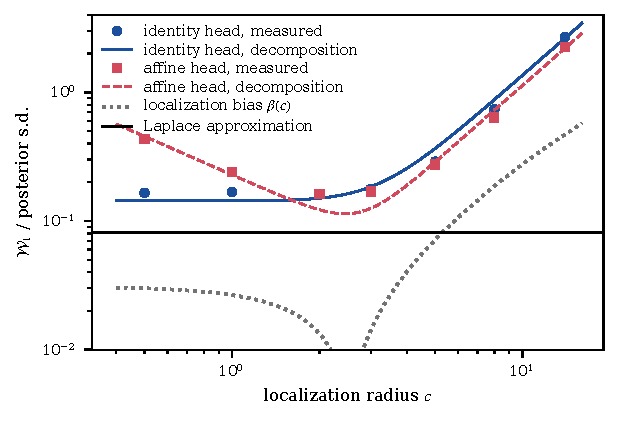
\includegraphics[width=0.9\textwidth]{mf_radius_theory}
\caption{The decomposition \eqref{m:eq:decomp} against measurement on the two dimensional Navier Stokes problem of Polson and Sokolov~\cite{polsonsokolov2026}, $D=6$, $M=1200$. Points are measured Wasserstein distances to an MCMC gold standard, in posterior standard deviations; curves are \eqref{m:eq:decomp} with $a_v$ and $b$ fitted separately for each head, and the bias $\beta(c)$ (dotted) is computed from \eqref{m:eq:bias} with no free parameter; the horizontal line is the Laplace approximation on the same run. The fitted optimum for the affine head is $c^\star=2.44$ against a measured optimum between $2$ and $3$; the root mean square residual of that fit is $0.044$. The localization bias is negligible below $c\approx3$, so in the fit of the affine head the left arm is estimation variance and the right arm nonlinearity. The identity head is the one produced by the study's script, whose residuals are neither centered at their sample mean nor rescaled, so that its flat left arm contains the displacement of Theorem~\ref{m:thm:locbias}(ii), which does not depend on $c$.}\label{m:fig:radius}
\end{figure}

Figure~\ref{m:fig:radius} tests \eqref{m:eq:decomp} on the Navier Stokes problem, with $a_v$ and $b$ fitted by least squares on the measured errors, which range from $0.16$ to $2.7$; the affine head's predicted optimum matches the measured one. The identity head's flat left arm is correctly predicted by $v=0$ (its level is mostly the displacement of Theorem~\ref{m:thm:locbias}(ii) and not the variance term), and the affine head's steep left arm by $v=2$: with a narrow proposal there is no design spread from which to estimate a slope.

\subsection{The design rule, and what it changes}

\begin{algorithm}[Localized GBC]\label{m:alg:loc}
Replace the step of Algorithm~\ref{m:alg:gbc} that simulates the training pairs by the following.
\begin{enumerate}[nosep]
\item Compute a preliminary estimate $\bar\theta_N$ and its Gauss Newton covariance $\Sigma_N$.
\item Draw $\theta^{(m)}\sim N(\bar\theta_N,c^2\Sigma_N)$ with $c\in[2,3]$, and simulate $Z^{(m)}$ from those.
\item Use the identity head with residuals centered at their sample mean (in the linear Gaussian model, equivalently, subtract $P\bar\theta_N$), and whiten by the sample covariance of the centered residuals rescaled by $(s_j+c^2p_j^2)^{-1/2}$ in the eigenbasis of $P$.
\item Do not add the residual mean to the center; do not use an affine head; do not importance weight back to the prior.
\end{enumerate}
\end{algorithm}

The radius $c\in[2,3]$ is not read off \eqref{m:eq:cstar}; the range is calibrated on the measurement, as Remark~\ref{m:rem:radiushead} sets out. Centering the residuals is Theorem~\ref{m:thm:locbias}(ii) and is the most consequential line of the algorithm; without it the generator carries a first order bias that no number of simulations removes. The rescaling is the second: without it the head reports the spread of the \emph{proposal} rather than of the posterior (Theorem~\ref{m:thm:locbias}(iii) and Remark~\ref{m:rem:rescale}). The prohibition on importance weighting is empirical and is explained by Theorem~\ref{m:thm:locbias}: the correction is unnecessary, because by Corollary~\ref{m:cor:locG}(i) there is no bias to remove once the residuals are centered and rescaled, while the weights $\pi/q_c$ are ratios of Gaussians with the wider density in the numerator and therefore have infinite variance whenever $c^2p_j\le1/2$ in some direction $j$, as in the data dominated directions here; in the Navier Stokes study the effective sample size never exceeded $34$ of $1200$ at any radius.

Algorithm~\ref{m:alg:loc} is a way of meeting (G1). Corollary~\ref{m:cor:locG} proves this in the linear Gaussian model. Localization is not new to the theory. The Bernstein von Mises theorems behind Theorem~\ref{m:thm:jwbvm} are proved on a localization set of the posterior, and Nickl and Wang~\cite{nicklwang2024}, in a steady state Schr\"odinger model, build their sampler on a surrogate log likelihood that agrees with the likelihood on a ball about a data driven initializer, of radius a small multiple of $D^{-4/d}$ with $D$ the dimension of their discretization, set by their stability estimate; only the training step had been left outside such a set.

\begin{corollary}[The localized design meets (G1) and (G2)]\label{m:cor:locG}
Consider the generator of Algorithm~\ref{m:alg:loc} with proposal $q_c=N(\bar\theta_N,c^2\Sigma_N)$ and $P=\Sigma_N\Sigma_0^{-1}$. In the setting of Lemma~\ref{m:lem:exact}, with $\Sigma_0$ and $\Phi^\top\Phi$ commuting as in Theorem~\ref{m:thm:locbias}:
\begin{enumerate}[label=(\roman*),nosep]
\item \emph{(Exactness in population.)} For every $c>0$ and every center $\bar\theta_N$, the law the head produces at the observed data is exactly the posterior, $N\big(S(Y),\Sigma_N\big)$. Localization contributes no bias at all, not merely a bias of smaller order.
\item \emph{(Finite $M$.)} With $M=M_N$ simulations and $J=J_N$ retained modes, the rescaled sample covariance of the centered residuals equals $\Sigma_N^{1/2}(\Id+\Delta_M)\Sigma_N^{1/2}$, where $\norm{\Delta_M}_{op}=O_P\big(\sqrt{J_N/M_N}+J_N/M_N\big)$ does not depend on $c$. Hence, when $\Sigma_{N,j}\lesssim\lambda_j/N$ on the retained modes ($\lambda_j$ the Laplace eigenvalues), as for the heat and Stokes equations, and $k>d/2$, $\Wone_{1,H^{-k-2}}(\Pihat,\PiN)=O_P\big(N^{-1/2}(\sqrt{J_N/M_N}+J_N/M_N)\big)$, so (G1) holds whenever $J_N/M_N\to0$, at every radius; and (G2) holds at every order whenever the exact posterior $N(S(Y),\Sigma_N)$ satisfies its first clause.
\item Consequently Theorem~\ref{m:thm:main} applies verbatim to Algorithm~\ref{m:alg:loc}, and Assumption~\ref{m:ass:G} is discharged for it.
\end{enumerate}
Part (i) does not use Assumption~\ref{m:ass:U}: in the linear Gaussian model the posterior given the summary is the posterior, so the two terms of Theorem~\ref{m:thm:qnnA} that need it vanish identically. Parts (ii) and (iii) quote the argument of Theorem~\ref{m:thm:qnnA}, and Remark~\ref{m:rem:u2pres} says what they need for a nonlinear forward map and what of it is open. Assumption~\ref{m:ass:u2p} itself is proved by Theorem~\ref{m:thm:u2ploc}, under the hypotheses there, for the uncentered and unrescaled head of Definition~\ref{m:def:gen}, so that Theorem~\ref{m:thm:qnnA} applies to that head under its other hypotheses.
\end{corollary}

\begin{proof}
(i) Write $A=\Sigma_NF$, so that $A+P=\Sigma_N(F+\Sigma_0^{-1})=\Id$, and $S=\Sigma_N\Phi^\top Y/\varsigma^2=A\theta+\Sigma_N\Phi^\top\varepsilon/\varsigma^2$. Hence
\[
R=\theta-S=P\theta-\Sigma_N\Phi^\top\varepsilon/\varsigma^2 ,
\]
which is Theorem~\ref{m:thm:locbias}: $E_{q_c}R=P\bar\theta_N$ and $\Var_{q_c}R=c^2P\Sigma_NP^\top+\Sigma_NF\Sigma_N$, equal to $\Sigma_{N,j}(s_j+c^2p_j^2)$ in the basis diagonalizing $P$. Subtracting the mean removes $P\bar\theta_N$ exactly, and dividing coordinate $j$ by $(s_j+c^2p_j^2)^{1/2}$ leaves variance exactly $\Sigma_{N,j}$; the rescaled residual is therefore $N(0,\Sigma_N)$, and the head returns $S(Y)+N(0,\Sigma_N)$, which by Lemma~\ref{m:lem:exact} is the exact posterior. What makes this work is not independence of $R$ and $S$, which fails under $q_c$: $\mathrm{Cov}_{q_c}(R,S)=(c^2P-\Id)\Sigma_NF\Sigma_N$, zero only when $c^2\Sigma_N=\Sigma_0$, as for the true prior. The head does not condition on $S$; it draws from the marginal law of the corrected residual and adds it to $S$, and that composition has the right conditional law because the corrected residual is $N(0,\Sigma_N)$ whatever $Y$ is.

(ii) Work in the basis diagonalizing $P$, $\Sigma_N$ and $F$, and let $V=\Var_{q_c}R$, diagonal with entries $\Sigma_{N,j}(s_j+c^2p_j^2)$ by (i). In the linear Gaussian model the residuals are $R^{(m)}=P\bar\theta_N+V^{1/2}g_m$ with $g_m$ i.i.d.\ $N(0,\Id_J)$, so the sample covariance of the centered residuals is $V^{1/2}(\Id+\Delta_M)V^{1/2}$, with $\Id+\Delta_M$ the sample covariance of the $g_m$; by the covariance estimation bound for Gaussian vectors~\cite[Theorem 4.7.1 and Exercise 4.7.3]{vershynin2018} with $u=J$, $\norm{\Delta_M}_{op}=O_P(\sqrt{J/M}+J/M)$, centering at the sample mean adding a term of rank one and of size $O_P(J/M)$. The rescaling is the diagonal matrix $Q$ with entries $(s_j+c^2p_j^2)^{-1/2}$, and $QV^{1/2}=\Sigma_N^{1/2}$, so the rescaled sample covariance is $\Sigma_N^{1/2}(\Id+\Delta_M)\Sigma_N^{1/2}$ and the radius drops out. The center of $\Pihat$ is $S(Y)$, as in (i), so coupling $\Pihat$ and $\PiN=N(S(Y),\Sigma_N)$ through a common $g\sim N(0,\Id_J)$ (Lemma~\ref{m:lem:coupling}) and using $|(1+x)^{1/2}-1|\le|x|$ for $x\ge-1$ gives
\[
\Wone_{1,H^{-k-2}}(\Pihat,\PiN)\le\big\|\Lambda^{-(k+2)/2}\Sigma_N^{1/2}\big\|_{HS}\,\norm{\Delta_M}_{op},
\]
where $\norm{\Lambda^{-(k+2)/2}\Sigma_N^{1/2}}^2_{HS}\le\sum_j\lambda_j^{-k-2}\Sigma_{N,j}\lesssim N^{-1}\sum_j\lambda_j^{-k-1}$ because $\Sigma_{N,j}\lesssim1/(N\iota_j)\lesssim\lambda_j/N$, and the sum is finite because $k>d/2$. For (G2), $\Pihat$ and $\PiN$ have the same center and the covariance of $\Pihat$ is at most $1+\norm{\Delta_M}_{op}$ times $\Sigma_N$, so the Gaussian concentration bounds in the proof of Theorem~\ref{m:thm:qnnA}, applied to either covariance, give spreads $O_P(r_N(s))$ in $H^s$. If $\PiN$ satisfies the first clause of (G2) with a constant $L$, then with probability above one half a draw from $\PiN$ lies in $\bar\Theta_{N,L}$, within $L\tilde\delta_N(0)$ of $S(Y)$ in $L^2$ and within $L$ of it in $H^{\bar\gamma}$, so $\norm{S(Y)-\theta_0}_{L^2}\le2L\tilde\delta_N(0)$ and $\norm{S(Y)}_{H^{\bar\gamma}}\le2L$ with probability tending to one, and the tail bound of that proof, with $L_1$ enlarged accordingly, gives (G2) for $\Pihat$ at every order.

(iii) is (i), (ii) and Theorem~\ref{m:thm:main}.
\end{proof}

\begin{remark}[Why the rescaling is not optional]\label{m:rem:rescale}
Without it the head reports $\sqrt{s_j+c^2p_j^2}$ times the correct posterior standard deviation in direction $j$, which is Theorem~\ref{m:thm:locbias}(iii). In the setting of Section~\ref{m:sec:expstudy}, $N=5\times10^4$ with $D=8$ retained modes of which $k_{\rm eff}=3$ are data dominated, the largest prior fraction is $p_{\max}=0.999$. The factor $\sqrt{1-p_j+c^2p_j^2}$ is at most one for every $p_j$ when $c=1$, so at that radius the unrescaled head \emph{understates} the posterior standard deviation, by at most $11\%$ over the eight modes, attained at $p_j=0.29$; for $c>1$ it overstates in every direction with $p_j>1/c^2$, by a factor that reaches $2.0$ at $c=2$, $3.0$ at $c=3$ and $8.0$ at $c=8$ in the most prior dominated direction.
\end{remark}

\begin{remark}[Which covariance the algorithm uses, and whether exactness survives it]\label{m:rem:whichcov}
$\Sigma_N$ in Algorithm~\ref{m:alg:loc} is $(F_{\bar\theta_N}+\Sigma_0^{-1})^{-1}$ with $F_{\bar\theta_N}$ the realized information $F_N$ of Remark~\ref{m:rem:reg}, that is the Gauss Newton information of the $N$ observations at the preliminary estimate, formed on the observed design. It is formed once and serves the proposal $c^2\Sigma_N$, the eigenbasis of $P$, and the factors $(s_j+c^2p_j^2)^{-1/2}$ alike; it is not reevaluated at the training draws, which is what keeps the cost at one Gauss Newton solve rather than $M$.

In the linear model nothing is plugged in, since $F=\Phi^\top\Phi/\varsigma^2$ does not depend on the point of evaluation; Corollary~\ref{m:cor:locG}(i) holds as stated. Nonlinearly it is a plug in and (i) does not survive verbatim. One thing does: one matrix serves both the proposal and the rescaling, so for the linearized residuals the correction $(s_j+c^2p_j^2)^{-1/2}$ undoes the inflation that produced them whatever $F_{\bar\theta_N}$ is. Two errors are left over. One is the discrepancy between $\Sigma_N(\bar\theta_N)$ and the Bernstein von Mises covariance, the same plug in error of order $\tilde\delta_N(\zeta)$ that Section~\ref{m:sec:qnn} bounds under the Lipschitz clause (U3). The other is the nonlinear remainder of the residuals under $q_c$, which Proposition~\ref{m:prop:locres} controls for a reused design. Granted the hypotheses that Remark~\ref{m:rem:u2pres} lists for parts (ii) and (iii), both enter (G1) additively alongside the $\sqrt{J_N/M_N}$ of (ii), and what is lost is the sharper reading of (i), that localization costs nothing at all rather than something of smaller order.
\end{remark}

\begin{remark}[The remaining term]\label{m:rem:relin}
In \eqref{m:eq:decomp} the term $b\,c^4$ arises because the summary is linearized once, at $\bar\theta_N$. Lemma~\ref{m:lem:exact} says that in the linear model the summary does not depend on the linearization point at all; the $c^4$ term is therefore purely a nonlinear effect, and it can be removed by iterating the Gauss Newton step and recomputing the Jacobian from the data alone at each iterate instead of once at $\bar\theta_N$, at a cost of $D+1$ forward solves per training draw for each extra step. Recomputing it at the training parameter $\theta^{(m)}$ would not define a statistic, since that parameter is not available for the observed data. The decomposition then reduces to $\beta(c)^2+a_v/c^v$, which for the affine head decreases in $c$ until the bias $\beta(c)$ begins to grow, so the optimal radius moves out to where the localization bias binds, and the achievable error is within $O(\sqrt{D/M})$ of the smallest value of $\beta(c)$, the floor it approaches as $M$ grows. Polson and Sokolov~\cite{polsonsokolov2026} carried this out with a two step Gauss Newton summary and confirmed that the $c^4$ term disappears; the error of the affine head at $c=6$ fell from $0.37$ to $0.16$ and became flat in $c$. After centering, the localized GBC posterior and the Laplace approximation agree with each other and with a $4500$ sample MCMC reference to the reference's own Monte Carlo error, $0.06$ posterior standard deviations. The cubic correction to the center, the first order shift $\frac12H^{-1}g$ of the posterior mean from the maximum a posteriori estimate, where $H$ is the negative Hessian of the log posterior density $\ell$ at the maximum and $g_a=\sum_{b,c}(H^{-1})_{bc}\,\partial_a\partial_b\partial_c\ell$ there, is at most $0.01$ standard deviations there, so the posterior is Gaussian in its center to that accuracy and neither method has anything left to correct in the well specified $T_0=0$ regime.
\end{remark}

\subsection{The whitened residuals of a localized proposal}\label{m:sec:u2ploc}

Everything is conditional on the data: $P$, $E$ and $\norm\cdot_{\psi_2}$ refer to the draw of the training pairs with $Z^{(N)}$ fixed, unless $P^\N_{\theta_0}$ is written. A simulated data set $Z^{(m)}$ is drawn from \eqref{m:eq:model} at $\theta^{(m)}$, with its own design points $X^{(m)}_i$, uniform on $\mathcal X$, and its own noise $\varepsilon^{(m)}_i\sim N(0,I_W)$, independent of each other and of $\theta^{(m)}$.

\emph{Notation.} Write $X$ for a uniform point of $\mathcal X$, $d_W$ for the dimension of an observation, $E_J=\mathrm{span}\{e_j:j\le J\}$, identified with $\R^J$, $P_J$ for the orthogonal projection onto it, $Q_J=\Id-P_J$, and $J=J_N$, so that $p_N=P_J$ in \eqref{m:eq:summary}. For a linear map $\mathcal T$ from $\ell^2$ into $\R^{d_W}$ valued functions on $\mathcal X$ let $\norm{\mathcal T}_{\ell^2\to L^2}=\sup_{\norm g_2\le1}(E\norm{(\mathcal Tg)(X)}^2_W)^{1/2}$. At a point $\vartheta$ where the linearization $\I_\vartheta$ is defined, define $K'_\vartheta$ by
\begin{equation}\label{m:eq:u2pF}
\langle f,(\Id+K'_\vartheta)g\rangle=E\big\langle(\I_\vartheta\mathcal D^{1/2}f)(X),(\I_\vartheta\mathcal D^{1/2}g)(X)\big\rangle_W ,
\end{equation}
that is $\Id+K'_\vartheta=T^{-1}\mathcal D^{1/2}\I^*_\vartheta\I_\vartheta\mathcal D^{1/2}$. Then $K'_{\theta_0}=K'$, $\norm{\I_\vartheta\mathcal D^{1/2}}^2_{\ell^2\to L^2}=\norm{\Id+K'_\vartheta}_{op}$, and $\Id+\Xi_\vartheta=P_J(\Id+K'_\vartheta)^{-1}P_J$. Fix a linearization point $\bar\vartheta$ determined by $Z^{(N)}$ at which $\Id+K'_{\bar\vartheta}$ is bounded and invertible, and let the training summary be \eqref{m:eq:summary} with one fold and the linearization point held at $\bar\vartheta$. It is linearized once, as in Remark~\ref{m:rem:relin}, but it uses the population information and carries no prior term, unlike the regularized summary of Lemma~\ref{m:lem:exact}: for $j\le J$,
\begin{equation}\label{m:eq:trainsummary}
\begin{aligned}
\hat S^{(m)}_{N,j}&=\langle e_j,\bar\vartheta\rangle\\
&\quad+\frac1N\sum_{i\le N}\Big\langle\I_{\bar\vartheta}\,p_N\big(\bar e_j^{\,\bar\vartheta}\big)(X^{(m)}_i),\;Y^{(m)}_i-u_{\bar\vartheta}(X^{(m)}_i)\Big\rangle_W .
\end{aligned}
\end{equation}
Since $\bar e_j^{\,\vartheta}=\mathcal D^{1/2}(\Id+K'_\vartheta)^{-1}\mathcal D^{1/2}e_j$ and $\mathcal D$ commutes with $P_J$, the whitened weights $\phi_j(x)=\iota_j^{1/2}\,\I_{\bar\vartheta}p_N(\bar e_j^{\,\bar\vartheta})(x)\in\R^{d_W}$ satisfy
\begin{equation}\label{m:eq:u2pW}
\sum_{j\le J}v_j\phi_j(x)=\big(\I_{\bar\vartheta}\mathcal D^{1/2}P_J(\Id+K'_{\bar\vartheta})^{-1}v\big)(x),\qquad v\in\R^J .
\end{equation}
Let $\phi(x)$ be the $J\times d_W$ matrix with rows $\phi_j(x)^\top$, so that the left side of \eqref{m:eq:u2pW} is $\phi(x)^\top v$, and write
\[
\begin{gathered}
G_\phi=E\,\phi(X)\phi(X)^\top,\qquad\hat G^{(m)}_\phi=\frac1N\sum_{i\le N}\phi(X^{(m)}_i)\phi(X^{(m)}_i)^\top,\\
b_J=\mathrm{ess\,sup}_x\norm{\phi(x)}^2_{op}
\end{gathered}
\]
for the Gram matrix of the whitened weights, its realized version and its envelope. Since $\norm{\phi\phi^\top}_F\le\norm\phi_{op}\norm\phi_F$, Chebyshev's inequality gives, for $t>0$ and the realized Gram matrix $\hat G_\phi$ of any $N$ independent uniform points of $\mathcal X$,
\begin{equation}\label{m:eq:u2pcheb}
\begin{aligned}
P\big(\norm{\hat G_\phi-G_\phi}_{op}>t\big)&\le t^{-2}E\norm{\hat G_\phi-G_\phi}^2_F\\
&\le\frac{E\norm{\phi(X)\phi(X)^\top}^2_F}{Nt^2}\le\frac{b_J\tr G_\phi}{Nt^2} .
\end{aligned}
\end{equation}
Substituting $Y^{(m)}_i=u_{\theta^{(m)}}(X^{(m)}_i)+\varepsilon^{(m)}_i$ in \eqref{m:eq:trainsummary} gives, for $v\in\R^J$,
\begin{equation}\label{m:eq:u2pdecomp}
\langle v,W^{(m)}\rangle=\mu_v-\frac1{\sqrt N}\sum_{i\le N}\big\langle\phi(X^{(m)}_i)^\top v,\varepsilon^{(m)}_i\big\rangle_W ,
\end{equation}
with $\mu_v$ a function of $Z^{(N)}$, $\theta^{(m)}$ and the design, so that conditionally on these $\langle v,W^{(m)}\rangle$ is normal with variance $v^\top\hat G^{(m)}_\phi v$.

\begin{lemma}[The Gram matrix of the whitened weights]\label{m:lem:u2pgram}
Let $\mathcal A=\Id+K'_{\bar\vartheta}$ be bounded on $\ell^2$ with $\mathcal A\succeq a\Id$ for some $a>0$, and write $B_J=\Id+\Xi_{\bar\vartheta}=P_J\mathcal A^{-1}P_J$. Then
\[
G_\phi=B_J+B_JP_J\mathcal AQ_J(Q_J\mathcal AQ_J)^{-1}Q_J\mathcal AP_JB_J ,
\]
so that $G_\phi\succeq B_J\succeq\norm{\mathcal A}^{-1}_{op}\Id$ and $\norm{G_\phi-B_J}_{op}\le a^{-3}\norm{K'_{\bar\vartheta}Q_J}^2_{op}$.
\end{lemma}

\begin{proof}
By \eqref{m:eq:u2pW} and \eqref{m:eq:u2pF}, $G_\phi=B_JP_J\mathcal AP_JB_J$ on $E_J$, and block inversion of $\mathcal A$ on $E_J\oplus Q_J\ell^2$ gives $B_J^{-1}=P_J\mathcal AP_J-P_J\mathcal AQ_J(Q_J\mathcal AQ_J)^{-1}Q_J\mathcal AP_J$; substituting gives the display, whose second term is positive semidefinite. Also $\mathcal A^{-1}\succeq\norm{\mathcal A}^{-1}_{op}\Id$, $\norm{Q_J\mathcal AP_J}_{op}=\norm{Q_JK'_{\bar\vartheta}P_J}_{op}\le\norm{K'_{\bar\vartheta}Q_J}_{op}$ by self adjointness, and $\norm{B_J}_{op}$ and $\norm{(Q_J\mathcal AQ_J)^{-1}}_{op}$ are at most $a^{-1}$.
\end{proof}

\begin{proposition}[No sub Gaussian envelope for the whole residual]\label{m:prop:u2pfalse}
Let each simulated data set have its own design, as in \eqref{m:eq:model}, let the training summary be \eqref{m:eq:trainsummary}, and let the training parameters have any law given $Z^{(N)}$. Then for every $N$, every $J$ and every unit vector $v\in\R^J$
\[
\begin{gathered}
\big\|\langle v,W^{(m)}\rangle\big\|^2_{\psi_2\mid Z^{(N)}}\ge2\,\mathrm{ess\,sup}_x\norm{\phi(x)^\top v}^2_W ,\\
\sup_{\norm u_2=1}\big\|\langle u,W^{(m)}\rangle\big\|^2_{\psi_2\mid Z^{(N)}}\ge2b_J\ge\frac{2\tr G_\phi}{d_W} .
\end{gathered}
\]
If $\Id+K'_{\bar\vartheta}$ is bounded and $\Id+K'_{\bar\vartheta}\succeq a\Id$ for some $a>0$, then $\tr G_\phi\ge J\norm{\Id+K'_{\bar\vartheta}}^{-1}_{op}$. For the heat and Stokes equations, observed from time zero as in \eqref{m:eq:model}, $G_\phi=\Id_J$ and $\norm{\langle e_J,W^{(m)}\rangle}^2_{\psi_2\mid Z^{(N)}}\ge2\norm{e_J}^2_{L^\infty}/\iota_J\ge2/\iota_J$, which grows like $\lambda_J$ by \eqref{m:eq:iota}; for the real trigonometric basis the bound is $4/\iota_J$.
\end{proposition}

\begin{proof}
Fix a unit vector $v$ and $s^2<\mathrm{ess\,sup}_x\norm{\phi(x)^\top v}^2_W$. The set $\mathcal X_s=\{x:\norm{\phi(x)^\top v}^2_W>s^2\}$ has positive measure, so with probability $P(X\in\mathcal X_s)^N>0$, whatever $\theta^{(m)}$ is, all $N$ design points lie in it, and then the conditional variance $\sigma^2=v^\top\hat G^{(m)}_\phi v$ in \eqref{m:eq:u2pdecomp} exceeds $s^2$. For $K^2<2s^2$ the exponent of $e^{x^2/K^2-(x-\mu_v)^2/(2\sigma^2)}$ then has a positive coefficient of $x^2$, so the conditional expectation of $e^{\langle v,W^{(m)}\rangle^2/K^2}$ given $Z^{(N)}$, $\theta^{(m)}$ and the design is infinite on an event of positive probability, and $\norm{\langle v,W^{(m)}\rangle}^2_{\psi_2\mid Z^{(N)}}\ge2s^2$. This is the first inequality. For the second, let $(v_k)$ be dense in the unit sphere of $\R^J$ and $c<b_J$. Each $x$ in the set $\{x:\norm{\phi(x)}^2_{op}>c\}$, which has positive measure, has $\norm{\phi(x)^\top v_k}^2_W>c$ for some $k$, so for some $k$ the set of such $x$ has positive measure, and the first inequality with $v=v_k$ gives $2c$. Next, $\norm{\phi(x)}^2_{op}\ge\norm{\phi(x)}^2_F/d_W$ and $\mathrm{ess\,sup}_x\norm{\phi(x)}^2_F\ge E\norm{\phi(X)}^2_F=\tr G_\phi$, and $\tr G_\phi\ge\tr(\Id+\Xi_{\bar\vartheta})\ge J\norm{\Id+K'_{\bar\vartheta}}^{-1}_{op}$ by Lemma~\ref{m:lem:u2pgram}. For the heat and Stokes equations $\I_\vartheta=\Lcal$ and $\Kcal=0$ in \eqref{m:eq:fredholm}, so $K'_{\bar\vartheta}=0$, $G_\phi=\Id_J$, and $\phi(t,x)^\top e_J=\iota_J^{-1/2}e^{-\nu\lambda_Jt}e_J(x)$ by \eqref{m:eq:modeinfo}, a continuous function whose squared norm has supremum $\norm{e_J}^2_{L^\infty}/\iota_J$, at $t=0$. The first inequality with $v=e_J$ gives the bound, and $\norm{e_J}^2_{L^\infty}\ge\int_\Omega\norm{e_J}^2_W=1$.
\end{proof}

For a nonlinear forward map three conditions on the linearization take the place of the explicit structure of the heat equation, and a fourth bounds its remainder. They involve a constant $a_\star>0$ and, for every $B>0$, constants $L_\star$, $C_\infty$ and $C_Q$ that may depend on $B$, and they are required for all $\vartheta,\vartheta'$ with $\norm\vartheta_{H^{\bar\gamma}},\norm{\vartheta'}_{H^{\bar\gamma}}\le B$:
\begin{enumerate}[label=(I\arabic*),nosep]
\item $\Id+K'_{\theta_0}$ is bounded on $\ell^2$, $K'_{\theta_0}$ is compact, and $\Id+K'_{\theta_0}\succeq a_\star\Id$;
\item $\norm{(\I_\vartheta-\I_{\theta_0})\mathcal D^{1/2}}_{\ell^2\to L^2}\le L_\star\norm{\vartheta-\theta_0}_{H^\zeta}$;
\item $\norm{\I_\vartheta h}_{L^\infty(\mathcal X)}\le C_\infty\norm h_{H^\zeta}$ for all $h\in H^\zeta$;
\item $\norm{u_{\vartheta'}-u_\vartheta-\I_\vartheta[\vartheta'-\vartheta]}_{L^\infty(\mathcal X)}\le C_Q\norm{\vartheta'-\vartheta}^2_{H^\zeta}$.
\end{enumerate}
Condition (I2) is a Lipschitz bound in the whitened $H^{-1}$ metric. It gives $\norm{\Xi_\vartheta-\Xi_{\theta_0}}_{op}\lesssim\norm{\vartheta-\theta_0}_{H^\zeta}$ for $\vartheta$ near $\theta_0$, uniformly in $J$, which the weight condition \eqref{m:eq:lipweight} does not, since its factor $\norm{e_j}_{H^{\kappa+2}}$ grows with $j$. Condition (I3) at $\vartheta=\theta_0$ is the second part of Condition 2D of Nickl~\cite{nicklbvm2024}. For Navier Stokes, (I1) is shown before Assumption~\ref{m:ass:u2p}, and Lemma~\ref{m:lem:nslin} proves (I2) to (I4).

\begin{theorem}[Assumption~\ref{m:ass:u2p} under a localized proposal]\label{m:thm:u2ploc}
Let $\bar\theta_N$ be a preliminary estimate as in Definition~\ref{m:def:summary}, let $J=J_N\asymp N^{d/(2\gamma+d)}$, and let the training parameters be
\[
\theta^{(m)}=\bar\theta_N+N^{-1/2}\mathcal D^{1/2}\mathcal V_N^{1/2}\xi^{(m)},
\]
where $\mathcal V_N$ is a positive semidefinite $J\times J$ matrix determined by $Z^{(N)}$ with $\norm{\mathcal V_N}_{op}=O_P(1)$, and the $\xi^{(m)}$ are i.i.d.\ standard normal on $\R^J$ given $Z^{(N)}$, conditioned on $\norm{\xi^{(m)}}^2_2\le4J$ when the forward map is nonlinear. Let the training summary be \eqref{m:eq:trainsummary} with $\bar\vartheta=\bar\theta_N$, and the generator that of Definition~\ref{m:def:gen}, uncentered and unrescaled.
\begin{enumerate}[label=(\alph*),nosep]
\item For the heat and Stokes equations, observed from time zero as in \eqref{m:eq:model}, with $\gamma>d+2$, which the hypotheses of Theorem~\ref{m:thm:qnnA} imply, Assumption~\ref{m:ass:u2p} holds with $\Xi=0$, $\varkappa_N\le4/\sqrt3$ and $W^{(m)}_{\rm g}=-1_{\mathcal B_m}N^{-1/2}\sum_i\phi(X^{(m)}_i)\varepsilon^{(m)}_i$, where $\mathcal B_m=\{\norm{\hat G^{(m)}_\phi-\Id}_{op}\le1\}$.
\item For a nonlinear forward map, Assumption~\ref{m:ass:u2p} holds under Conditions 1 and 2 of Nickl~\cite{nicklbvm2024} with the constants of Theorem~\ref{m:thm:nickl2}, $\bar\gamma<\gamma-1$, the rate hypothesis $\sqrt N\,\tilde\delta_N(0)\tilde\delta_N(\zeta)\to0$ of Proposition~\ref{m:prop:suff}, and (I1) to (I3).
\item Let $\Sigma_0$ be positive definite, $\Sigma_N=(F_{\bar\theta_N}+\Sigma_0^{-1})^{-1}$ with $F_{\bar\theta_N}$ the realized information on $J$ modes (Remark~\ref{m:rem:whichcov}), and $a_\star=1$ in (a). Under the hypotheses of (a) or (b), with probability tending to one $N^{-1}\mathcal D^{1/2}F_{\bar\theta_N}\mathcal D^{1/2}\succeq(a_\star/12)\Id$, and then $\mathcal V_N=c^2N\mathcal D^{-1/2}\Sigma_N\mathcal D^{-1/2}$ has $\norm{\mathcal V_N}_{op}\le12c^2/a_\star$.
\end{enumerate}
\end{theorem}

The proposal $N(\bar\theta_N,c^2\Sigma_N)$ of Algorithm~\ref{m:alg:loc} on $D=J$ modes has this form with $\mathcal V_N=c^2N\mathcal D^{-1/2}\Sigma_N\mathcal D^{-1/2}$, and part (c) gives $\norm{\mathcal V_N}_{op}=O_P(1)$. For the heat and Stokes equations $N^{-1}\mathcal D^{1/2}F_{\bar\theta_N}\mathcal D^{1/2}$ is the realized Gram matrix $\hat G_\phi$ of the observed design, which tends to $\Id$ by \eqref{m:eq:u2pcheb}, since $b_JJ/N\to0$ (Step 5 below). Since $P(\norm\xi^2_2>4J)\le(4e^{-3})^{J/2}$, truncated and untruncated draws coincide except on an event of probability at most $M(4e^{-3})^{J/2}$, which tends to zero when $\log M_N=o(J_N)$. If instead the simulated data sets reuse the observed design $(X_i)_{i\le N}$ and draw only fresh noise, as in Lemma~\ref{m:lem:exact}, then for the heat and Stokes equations the computation of Step 1 below gives $W^{(m)}=-(\hat G_\phi-\Id)\mathcal V_N^{1/2}\xi^{(m)}-N^{-1/2}\sum_i\phi(X_i)\varepsilon^{(m)}_i$, which is centered Gaussian given $Z^{(N)}$ with covariance $(\hat G_\phi-\Id)\mathcal V_N(\hat G_\phi-\Id)+\hat G_\phi$. Since $\hat G_\phi\to\Id$, Assumption~\ref{m:ass:u2p} then holds with $W^{(m)}_{\rm r}=0$, and the whole residual has a sub Gaussian norm bounded uniformly in $J$ with probability tending to one.

\begin{proof}
In (a) the bounds below depend on $Z^{(N)}$ only through $\norm{\mathcal V_N}_{op}$. In (b) the events $A_N$ on which $\norm{\mathcal V_N}_{op}\le c_{\mathcal V}$, $\norm{\bar\theta_N}_{H^{\bar\gamma}}\le B$, $\norm{\bar\theta_N-\theta_0}_{H^\zeta}\le L\tilde\delta_N(\zeta)$ and $\norm{\bar\theta_N-\theta_0}_{L^2}\le L\tilde\delta_N(0)$ have probability tending to one as $c_{\mathcal V},B,L\to\infty$, uniformly in large $N$, by Definition~\ref{m:def:summary}. Let $\eta_N$ be the sum of the two quantities in the second display of Assumption~\ref{m:ass:u2p}. It suffices to show that for fixed constants, with $Z^{(N)}$ fixed, $\norm{\mathcal V_N}_{op}\le c_{\mathcal V}$ in (a) and $A_N$ in force in (b), $\varkappa_N$ is bounded and $\eta_N$ is at most a deterministic sequence that tends to zero. We drop the index $m$.

\emph{Step 1: decomposition.} Write $\mathcal A=\Id+K'_{\bar\theta_N}$, $\mathcal A_0=\Id+K'_{\theta_0}$, $\tilde h=\mathcal V_N^{1/2}\xi\in E_J$, $h=\theta-\bar\theta_N=N^{-1/2}\mathcal D^{1/2}\tilde h$ and $\tilde u=\I_{\theta_0}\mathcal D^{1/2}\tilde h$. With $R_0(\vartheta)=u_\vartheta-u_{\theta_0}-\I_{\theta_0}[\vartheta-\theta_0]$ we have $u_\theta-u_{\bar\theta_N}=N^{-1/2}\tilde u+r_\theta$, where $r_\theta=R_0(\theta)-R_0(\bar\theta_N)$ vanishes for a linear map, and substituting $Y_i=u_\theta(X_i)+\varepsilon_i$ in \eqref{m:eq:trainsummary} gives
\[
\begin{aligned}
W&=\tilde h-\frac1N\sum_i\phi(X_i)\tilde u(X_i)\\
&\quad-\frac1{\sqrt N}\sum_i\phi(X_i)r_\theta(X_i)-\frac1{\sqrt N}\sum_i\phi(X_i)\varepsilon_i .
\end{aligned}
\]
By \eqref{m:eq:u2pW}, the summands of the first sum have mean $P_J\mathcal A^{-1}P_JT^{-1}\mathcal D^{1/2}\I^*_{\bar\theta_N}\I_{\theta_0}\mathcal D^{1/2}\tilde h$ over $X$, and writing $\tilde h=P_J\mathcal A^{-1}\mathcal A\tilde h$ with $Q_J\mathcal A\tilde h=Q_JK'_{\bar\theta_N}\tilde h$ shows that $\tilde h$ minus this mean is $\mathcal C\tilde h$, where
\[
\mathcal C=P_J\mathcal A^{-1}Q_JK'_{\bar\theta_N}P_J+P_J\mathcal A^{-1}P_JT^{-1}\mathcal D^{1/2}\I^*_{\bar\theta_N}\big(\I_{\bar\theta_N}-\I_{\theta_0}\big)\mathcal D^{1/2}P_J .
\]
With the design event $\mathcal B=\{\norm{\hat G_\phi-G_\phi}_{op}\le1\}$ set
\[
\begin{aligned}
W_{\rm g}&=\mathcal C\tilde h-1_{\mathcal B}\frac1{\sqrt N}\sum_i\phi(X_i)\varepsilon_i ,\\
W_{\rm r}&=-1_{\mathcal B^c}\frac1{\sqrt N}\sum_i\phi(X_i)\varepsilon_i-\Big(\frac1N\sum_i\phi(X_i)\tilde u(X_i)-E\,\phi(X)\tilde u(X)\Big)\\
&\quad-\frac1{\sqrt N}\sum_i\phi(X_i)r_\theta(X_i),
\end{aligned}
\]
the expectation in the middle term taken over $X$ with $\tilde h$ fixed. Then $W=W_{\rm g}+W_{\rm r}$, the pairs $(W_{\rm g},W_{\rm r})$ are i.i.d.\ over the simulations given $Z^{(N)}$, and $E\,W_{\rm g}=0$, because $\xi$ is symmetric and the noise is centered and independent of $\xi$ and of the design.

\emph{Step 2: the sub Gaussian part.} Given the design and $\xi$, the variable $1_{\mathcal B}N^{-1/2}\sum_i\langle\phi(X_i)^\top v,\varepsilon_i\rangle_W$ is centered normal with variance at most $s^2=\norm{G_\phi}_{op}+1$ for unit $v$, and a centered normal variable $\chi$ with variance at most $s^2$ has $E\,e^{\chi^2/K^2}\le(1-2s^2/K^2)^{-1/2}=2$ at $K^2=8s^2/3$, so its sub Gaussian norm is at most $(8/3)^{1/2}s$. For the other term, $\langle v,\mathcal C\tilde h\rangle=\langle\mathcal V_N^{1/2}\mathcal C^\top v,\xi\rangle$, and every $\langle u,\xi\rangle$ with $\norm u_2=1$ has sub Gaussian norm at most $2\sqrt3$: $E\,e^{\langle u,\xi\rangle^2/12}=(5/6)^{-1/2}$ for the standard normal law, and conditioning on $\{\norm\xi^2_2\le4J\}$, an event of probability at least $1-(4e^{-3})^{J/2}\ge0.55$ by the Chernoff bound $P(\norm\xi^2_2\ge4J)\le e^{-3J/2}E\,e^{3\norm\xi^2_2/8}$, raises this to at most $(5/6)^{-1/2}/0.55<2$. Hence
\[
\varkappa_N\le(8/3)^{1/2}\big(\norm{G_\phi}_{op}+1\big)^{1/2}+2\sqrt3\,c_{\mathcal V}^{1/2}\norm{\mathcal C}_{op} .
\]

\emph{Step 3: the second moment.} The two terms of $W_{\rm g}$ are uncorrelated, since the second is centered given $\xi$ and the design, and $E\,\xi\xi^\top\preceq\Id$, since the truncation preserves rotation invariance and does not raise $E\norm\xi^2_2$. Hence $E\,W_{\rm g}W_{\rm g}^\top=E\,\mathcal C\tilde h\tilde h^\top\mathcal C^\top+G_\phi-E\,\hat G_\phi1_{\mathcal B^c}$, where the first term has norm at most $c_{\mathcal V}\norm{\mathcal C}^2_{op}$ and the last at most $b_JP(\mathcal B^c)\le b_J^2\tr G_\phi/N$ by \eqref{m:eq:u2pcheb}. With Lemma~\ref{m:lem:u2pgram}, $a$ a lower bound for $\mathcal A$, and $\norm{\Xi_{\bar\theta_N}-\Xi_{\theta_0}}_{op}\le\norm{\mathcal A^{-1}-\mathcal A_0^{-1}}_{op}$, this gives
\[
\begin{aligned}
\big\|E\,W_{\rm g}W_{\rm g}^\top-(\Id+\Xi)\big\|_{op}&\le c_{\mathcal V}\norm{\mathcal C}^2_{op}+\frac{b_J^2\tr G_\phi}N\\
&\quad+\frac{\norm{K'_{\bar\theta_N}Q_J}^2_{op}}{a^3}+\norm{\mathcal A^{-1}-\mathcal A_0^{-1}}_{op} .
\end{aligned}
\]

\emph{Step 4: the remainder.} Given the design, the first term of $W_{\rm r}$ has second moment $1_{\mathcal B^c}\tr\hat G_\phi\le1_{\mathcal B^c}d_Wb_J$. Given $\xi$, the middle term is an average of $N$ i.i.d.\ centered vectors, with second moment at most $N^{-1}E\norm{\phi(X)}^2_{op}\norm{\tilde u(X)}^2_W\le N^{-1}b_J\langle\tilde h,\mathcal A_0\tilde h\rangle$. Given $\theta$, the last term has second moment at most $E\norm{\phi(X)r_\theta(X)}^2_2+N\norm{E\,\phi(X)r_\theta(X)}^2_2\le(b_J+N\norm{G_\phi}_{op})E\norm{r_\theta(X)}^2_W$, because $\norm{E\,\phi r_\theta}_2=\sup_{\norm v_2=1}E\langle\phi^\top v,r_\theta\rangle_W\le\norm{G_\phi}^{1/2}_{op}(E\norm{r_\theta}^2_W)^{1/2}$. With \eqref{m:eq:u2pcheb} and $E\norm{\tilde h}^2_2\le c_{\mathcal V}J$ this gives
\[
\begin{aligned}
E\norm{W_{\rm r}}^2_2&\le\frac{3d_Wb_J^2\tr G_\phi}N+\frac{3c_{\mathcal V}b_J\norm{\mathcal A_0}_{op}J}N\\
&\quad+3\big(b_J+N\norm{G_\phi}_{op}\big)\sup_\theta E\norm{r_\theta(X)}^2_W ,
\end{aligned}
\]
the supremum taken over the support of the proposal.

\emph{Step 5: the heat and Stokes equations.} Here $K'_\vartheta=0$, $\I_\vartheta=\Lcal$ and $r_\theta=0$, so $\mathcal C=0$, $\mathcal A=\mathcal A_0=G_\phi=\Id$, $\Xi=0$ and $\varkappa_N\le(16/3)^{1/2}=4/\sqrt3$. The weights are $\phi_j(t,x)=\iota_j^{-1/2}e^{-\nu\lambda_jt}e_j(x)$ with $\norm{e_j(x)}^2_W\le2$, and $\iota_j^{-1}\le1+2\nu\lambda_jT$ by \eqref{m:eq:iota} at $T_0=0$, so $b_J\le2\sum_{j\le J}\iota_j^{-1}\lesssim J\lambda_J\asymp J^{1+2/d}$. Steps 3 and 4 bound $\eta_N$ by a constant times $b_J^2J/N\lesssim N^{(3d+4)/(2\gamma+d)-1}$, which tends to zero because $\gamma>d+2$. The hypotheses of Theorem~\ref{m:thm:qnnA} give $\gamma>3\zeta+3d/2+2$ with $\zeta>d/2$, hence $\gamma>3d+2$. This proves (a).

\emph{Step 6: a nonlinear map.} By (I2), $\upsilon_N=\norm{(\I_{\bar\theta_N}-\I_{\theta_0})\mathcal D^{1/2}}_{\ell^2\to L^2}\le L_\star L\tilde\delta_N(\zeta)\to0$. Since $\mathcal A-\mathcal A_0$ is the difference of the forms \eqref{m:eq:u2pF} at $\bar\theta_N$ and at $\theta_0$, $\norm{\mathcal A-\mathcal A_0}_{op}\le\upsilon_N(2\norm{\mathcal A_0}^{1/2}_{op}+\upsilon_N)\to0$, so for $N$ large $\mathcal A\succeq(a_\star/2)\Id$, $\norm{\mathcal A^{-1}-\mathcal A_0^{-1}}_{op}\le2a_\star^{-2}\norm{\mathcal A-\mathcal A_0}_{op}\to0$, and $\norm{K'_{\bar\theta_N}Q_J}_{op}\le\norm{K'_{\theta_0}Q_J}_{op}+\norm{\mathcal A-\mathcal A_0}_{op}\to0$, the first term because $K'_{\theta_0}$ is compact and self adjoint by (I1). Since $P_J\mathcal A^{-1}Q_J=-P_J\mathcal A^{-1}K'_{\bar\theta_N}Q_J$,
\[
\norm{\mathcal C}_{op}\le\frac2{a_\star}\Big(\norm{K'_{\bar\theta_N}Q_J}^2_{op}+\norm{\mathcal A}^{1/2}_{op}\,\upsilon_N\Big)\to0 ,
\]
while $\norm{G_\phi}_{op}\le2/a_\star+8a_\star^{-3}\norm{K'_{\bar\theta_N}Q_J}^2_{op}$ stays bounded by Lemma~\ref{m:lem:u2pgram}, so $\varkappa_N$ is bounded. By (I3) and \eqref{m:eq:u2pW}, $\norm{\phi(x)^\top v}_W\le C_\infty\norm{\mathcal D^{1/2}P_J\mathcal A^{-1}v}_{H^\zeta}\le C_\infty(2/a_\star)\max_{j\le J}(1+\lambda_j)^{\zeta/2}\iota_j^{-1/2}\norm v_2$, so $b_J\lesssim\lambda_J^{\zeta+1}$ and $b_J^2J/N\lesssim N^{(4\zeta+4+d)/(2\gamma+d)-1}\to0$, because $\gamma>3\zeta+3d/2+2>2\zeta+2$ by the hypotheses of Theorem~\ref{m:thm:nickl2}. It remains to bound $r_\theta$. On the support of the proposal, for $s\ge0$,
\[
\norm h^2_{H^s}\le\frac{4c_{\mathcal V}J}N\max_{j\le J}(1+\lambda_j)^s\iota_j^{-1}\lesssim\frac{J\lambda_J^{s+1}}N ,
\]
which tends to zero for $s=\bar\gamma$ because $\bar\gamma<\gamma-1$. So for $N$ large both $\theta-\theta_0$ and $\bar\theta_N-\theta_0$ lie in $U(\bar\gamma,B+\norm{\theta_0}_{H^{\bar\gamma}}+1)$, and Condition 2C, applied to each of the two terms of $r_\theta$, gives
\[
\big(E\norm{r_\theta(X)}^2_W\big)^{1/2}\lesssim\norm{\theta-\theta_0}^2_{L^2}+\norm{\bar\theta_N-\theta_0}^2_{L^2}\lesssim\tilde\delta_N(0)^2+\frac{J\lambda_J}N .
\]
Since $\tilde\delta_N(0)\le\tilde\delta_N(\zeta)$, the rate hypothesis gives $N\tilde\delta_N(0)^4\to0$, and $N(J\lambda_J/N)^2\asymp N^{(2d+4)/(2\gamma+d)-1}\to0$ because $\gamma>2+d/2$; also $b_J\lesssim N$. Steps 2 to 4 now give (b).

\emph{Step 7: part (c).} Let $\bar\theta_N$ be computed from $Z^{[b]}$, let $n\ge N/3$ be the size of the other half $\mathcal I_{3-b}$, and let $\psi(x)$ be the $J\times d_W$ matrix with rows $\iota_j^{-1/2}(\I_{\bar\theta_N}e_j)(x)^\top$, so that $N^{-1}\mathcal D^{1/2}F_{\bar\theta_N}\mathcal D^{1/2}\succeq(n/N)\hat G_\psi$ with $\hat G_\psi=n^{-1}\sum_{i\in\mathcal I_{3-b}}\psi(X_i)\psi(X_i)^\top$. Given $Z^{[b]}$ these $X_i$ are independent and uniform, and $E\,\psi(X)\psi(X)^\top=P_J\mathcal AP_J\succeq(a_\star/2)\Id$ by \eqref{m:eq:u2pF}, with $\mathcal A=\Id$ in (a) and, in (b), by Step 6 on the part of $A_N$ that concerns $\bar\theta_N$ and for $N$ large, where also $\norm{\mathcal A}_{op}\le\norm{\mathcal A_0}_{op}+1$. By Step 5 in (a) and by (I3) in (b), $b_\psi=\mathrm{ess\,sup}_x\norm{\psi(x)}^2_{op}$ is $O(J\lambda_J)$ and $O(\lambda_J^{\zeta+1})$, so \eqref{m:eq:u2pcheb} for $\psi$ with $t=a_\star/4$ bounds the probability that $\hat G_\psi\not\succeq(a_\star/4)\Id$ by $16b_\psi J\norm{\mathcal A}_{op}/(a_\star^2n)$, which tends to zero as in Steps 5 and 6. As $n/N\ge1/3$ and $\Sigma_N\preceq F_{\bar\theta_N}^{-1}$, (c) follows.
\end{proof}

\begin{lemma}[The linearization of the reaction diffusion class]\label{m:lem:rdlin}
In the setting of Theorem~\ref{m:thm:nickl1}, with $\theta_0\in C^\infty$, $K_f=\sup|f'|$ and $\I_\vartheta h$ the solution $U$ of $\partial_tU=\Delta U+f'(u_\vartheta)U$, $U(0)=h$, conditions (I1) to (I4) hold for every $\zeta>d/2$ and every $\bar\gamma>\max(1,\zeta)$, and $\norm{\Id+K'_\vartheta}_{op}$ is bounded by a constant that depends only on $K_f$ and $T$.
\end{lemma}

\begin{proof}
Write $\norm\cdot$ for the norm of $L^2(\Omega)$, $\norm g^2_{-1}=\langle(\Id-\Delta)^{-1}g,g\rangle$, which is the norm of $H^{-1}$ in the convention (13) of Nickl~\cite{nicklbvm2024}, and $V=f'(u_\vartheta)$, so that $|V|\le K_f$. By \eqref{m:eq:iota} with $\nu=1$ and $T_0=0$, $\iota_j(1+\lambda_j)$ lies between two positive constants that depend only on $T$, so $\norm{\mathcal D^{-1/2}g}_2$ and $\norm g_{-1}$ are equivalent norms, and since $|\Omega|=1$, $E\norm{(\I_\vartheta h)(X)}^2=T^{-1}\int_0^T\norm{\I_\vartheta h(t)}^2dt$. We prove the bounds for $h\in H^1$, for which the weak solutions of (108) of Nickl~\cite{nicklbvm2024} exist with $U\in L^2([0,T],H^1)$ and $\partial_tU\in L^2([0,T],H^{-1})$, and extend them by density.

\emph{Upper bound.} Testing (108) there with $(\Id-\Delta)^{-1}U(t)$ and using $\norm{(\Id-\Delta)^{-1}U}\le\norm U_{-1}$,
\[
\begin{aligned}
\tfrac12\tfrac d{dt}\norm U^2_{-1}&=-\norm U^2+\norm U^2_{-1}+\langle VU,(\Id-\Delta)^{-1}U\rangle\\
&\le-\tfrac12\norm U^2+\big(1+\tfrac12K_f^2\big)\norm U^2_{-1} .
\end{aligned}
\]
Gr\"onwall's inequality gives $\norm{U(t)}^2_{-1}\le e^{(2+K_f^2)t}\norm h^2_{-1}$, and integrating the inequality over $[0,T]$ then gives $\int_0^T\norm{U(t)}^2dt\le e^{(2+K_f^2)T}\norm h^2_{-1}$, a bound that does not depend on $\vartheta$.

\emph{Compactness.} Let $\mathcal Z$ be the Duhamel operator $(\mathcal Zw)(t)=\int_0^te^{(t-s)\Delta}w(s)\,ds$ on $L^2([0,T],L^2(\Omega))$. On the coefficient of $e_j$ it is convolution in time with $e^{-\lambda_jr}1_{r>0}$, a compact operator on $L^2[0,T]$ of norm at most $\min(T,\lambda_j^{-1})$ by Young's inequality, so $\mathcal Z$ is the limit in operator norm of its compact truncations to finitely many modes, and is compact. The weak solution is the mild solution $U=\Lcal h+\mathcal Z(VU)$, so $\I_\vartheta\mathcal D^{1/2}=\Lcal\mathcal D^{1/2}+\mathcal Z\,V\,\I_\vartheta\mathcal D^{1/2}$ with the second operator compact. Since $\Lcal\mathcal D^{1/2}$ is an isometry from $\ell^2$ into $L^2$ of the uniform probability on $\mathcal X$, by \eqref{m:eq:modeinfo}, expanding \eqref{m:eq:u2pF} shows that $K'_\vartheta$ is compact.

\emph{Lower bound at $\theta_0$.} The potential $f'(u_{\theta_0})$ lies in $C^1([0,T],C^1)$ for smooth $\theta_0$, by Proposition~4 of Nickl~\cite{nicklbvm2024}, and Lemma~4 there gives $\int_0^T\norm{U(s)}^2ds\ge c\norm h^2_{H^{-1}}$ for $h\in H^1$, where $\norm h_{H^{-1}}$ is bounded below by a constant times $\norm h_{-1}$, since the dual norms (16) there are equivalent to the norms (13) there for negative exponents. With the upper bound and density this gives $\Id+K'_{\theta_0}\succeq a_\star\Id$ for some $a_\star>0$, and (I1) holds.

\emph{(I2).} Let $U=\I_\vartheta h$, $U_0=\I_{\theta_0}h$, $V_0=f'(u_{\theta_0})$ and $\delta U=U-U_0$, which solves $\partial_t\delta U=\Delta\delta U+V\delta U+(V-V_0)U_0$, $\delta U(0)=0$. Testing with $\delta U$ gives $\tfrac d{dt}\norm{\delta U}^2\le(2K_f+1)\norm{\delta U}^2+\norm{V-V_0}^2_{L^\infty(\mathcal X)}\norm{U_0}^2$, and Gr\"onwall's inequality with the upper bound gives
\[
\int_0^T\norm{\delta U(t)}^2dt\le Te^{(2K_f+1)T}e^{(2+K_f^2)T}\norm{V-V_0}^2_{L^\infty(\mathcal X)}\norm h^2_{-1} .
\]
By the mean value theorem and (103) of Nickl~\cite{nicklbvm2024}, $\norm{V-V_0}_{L^\infty(\mathcal X)}\le\sup|f''|\sup_{0<t<T}\norm{u_\vartheta(t)-u_{\theta_0}(t)}_\infty\lesssim\norm{\vartheta-\theta_0}_{H^\zeta}$, with a constant that depends on $f$ and on a bound for $\norm\vartheta_{H^\zeta}+\norm{\theta_0}_{H^\zeta}$, which $\norm\vartheta_{H^{\bar\gamma}}\le B$ supplies because $\bar\gamma>\zeta$. With $h=\mathcal D^{1/2}g$ this is (I2).

\emph{(I3).} Write $\mathcal Z_Vw=\mathcal Z(Vw)$, so that the mild solution is the series $U=\sum_{n\ge0}\mathcal Z_V^n\Lcal h$. The heat semigroup is positive and satisfies $e^{(t-s)\Delta}e^{s\Delta}=e^{t\Delta}$, so induction gives $|(\mathcal Z_V^n\Lcal h)(t)|\le(K_ft)^n(n!)^{-1}e^{t\Delta}|h|$ pointwise. The series therefore converges uniformly on $\mathcal X$, its sum is the mild solution, which is unique because the powers $\mathcal Z_V^n$ have norms at most $(K_fT)^n/n!$, and $|U(t,x)|\le e^{K_fT}\norm h_\infty$. Finally, since $\norm{e_j}_\infty\le\sqrt2$, $\norm h_\infty\le\sqrt2\sum_j|\langle h,e_j\rangle|\le\big(2\sum_j(1+\lambda_j)^{-\zeta}\big)^{1/2}\norm h_{H^\zeta}$, finite for $\zeta>d/2$.

\emph{(I4).} With $w=u_{\vartheta'}-u_\vartheta$ and $V=f'(u_\vartheta)$, the mild form of the equations gives $z=w-\I_\vartheta[\vartheta'-\vartheta]$ as $z(t)=\int_0^te^{(t-s)\Delta}(Vz+q)(s)\,ds$, where $|q|=|f(u_{\vartheta'})-f(u_\vartheta)-Vw|\le\frac12\sup|f''|\,w^2$. The heat semigroup does not increase the supremum norm, and $z$ is bounded by (103) of Nickl~\cite{nicklbvm2024} and (I3), so Gr\"onwall's inequality and (103) give $\norm z_{L^\infty(\mathcal X)}\lesssim\sup_t\norm{w(t)}^2_\infty\lesssim\norm{\vartheta'-\vartheta}^2_{H^\zeta}$.
\end{proof}

\begin{lemma}[The linearization of the Navier Stokes equations]\label{m:lem:nslin}
For the Navier Stokes equations of Section~\ref{m:sec:ns} with $f\in\Hds{1}$ and $\theta_0\in\Hds{2}$, conditions (I2) to (I4) hold with $\zeta=2$ for every $\bar\gamma\ge2$. If moreover $f,\theta_0\in\Hds{\infty}$, as in Theorem~2.11 of Konen and Nickl~\cite{konennickl2026}, then with (I1), and with Condition 2C from their Proposition~3.8(iii), every hypothesis of Theorem~\ref{m:thm:u2ploc}(b) on the forward map holds, with their Condition 2.12 in place of Condition 2 and $\gamma=\alpha>12>3\zeta+3d/2+2$.
\end{lemma}

\begin{proof}
We use the homogeneous norms of Konen and Nickl~\cite{konennickl2026}, with $\norm\cdot_{\Hds{a}}\le\norm\cdot_{H^a}$ for $a\ge0$, and their Propositions~3.4, 3.7, 3.9, 3.12 and~4.1 with $a\in\{-1,2\}$, where $a^*=2$; the constants depend on $\nu$, $T$, $\norm f_{\Hds{1}}$ and $L=2(B+\norm{\theta_0}_{\Hds{2}})$, which bounds the $\Hds{2}$ norms of the initial conditions. For $h\in\Hds{1}$, by their Proposition~3.8(ii), $\delta U=\I_\vartheta[h]-\I_{\theta_0}[h]$ solves their equation (4.4) with $\theta=\theta'=\vartheta$, $\xi=0$ and $g=-B[w,U_0]-B[U_0,w]$, where $w=u_\vartheta-u_{\theta_0}$ and $U_0=\I_{\theta_0}[h]$, and, lying in $C([0,T],\Hds{1})\cap L^2([0,T],\Hds{2})$ by their Proposition~3.9 with $a=1$, it is the unique solution of their Proposition~4.1 with $a=-1$, which gives the first inequality in $\int_0^T\norm{\delta U}^2_{L^2}dt\lesssim\int_0^T\norm g^2_{\Hds{-2}}dt\lesssim\norm{\vartheta-\theta_0}^2_{\Hds{2}}\norm h^2_{\Hds{-1}}$, and their Proposition~3.4 with $a=-1$, the Poincar\'e inequality and their Propositions~3.7 with $a=2$ and~3.9 with $a=-1$ give the second. The bound extends to $h\in\Hds{-1}$ by density, and since $E\norm{\delta U(X)}^2=T^{-1}\int_0^T\norm{\delta U}^2_{L^2}dt$ and $\norm{\mathcal D^{1/2}v}^2_{\Hds{-1}}=\sum_jv_j^2/(\lambda_j\iota_j)\le2\nu T\norm v^2_2/(1-e^{-2\nu\lambda_1T})$ by \eqref{m:eq:iota}, it is (I2). Their Propositions~3.9 and~3.12 with $a=2$ bound $\sup_t\norm{\I_\vartheta[h](t)}_{\Hds{2}}$ by a multiple of $\norm h_{\Hds{2}}$, and $\sup_t\norm{u_{\vartheta'}(t)-u_\vartheta(t)-\I_\vartheta[\vartheta'-\vartheta](t)}_{\Hds{2}}$ by a multiple of $\norm{\vartheta'-\vartheta}^2_{\Hds{2}}$, and $\Hds{2}\subset C(\Omega)^2$ gives (I3) and (I4).
\end{proof}

\begin{remark}[The centered and rescaled residuals of Algorithm~\ref{m:alg:loc}]\label{m:rem:u2pres}
Theorem~\ref{m:thm:u2ploc} concerns the head of Definition~\ref{m:def:gen} with the summary \eqref{m:eq:trainsummary}. That head needs neither correction of step~3 of Algorithm~\ref{m:alg:loc}: $E\,W^{(m)}=E\,W^{(m)}_{\rm r}$ tends to zero, and $E[W^{(m)}W^{(m)\top}\mid Z^{(N)}]$ tends to $\Id+\Xi$ at every fixed radius, since Theorem~\ref{m:thm:u2ploc} holds for every $\mathcal V_N$ with $\norm{\mathcal V_N}_{op}=O_P(1)$ and the radius enters only through $\mathcal V_N$. The corrections belong to the regularized summary of Lemma~\ref{m:lem:exact}, and for its centered and rescaled residuals Assumption~\ref{m:ass:u2p} is not the right hypothesis. In the setting of Corollary~\ref{m:cor:locG} for the heat and Stokes equations, where $\Xi=0$, the centered and rescaled residual is exactly $N(0,\Sigma_N)$ by part (i) there, so its whitened second moment matrix is $N\mathcal D^{-1/2}\Sigma_N\mathcal D^{-1/2}$, whose $J$th diagonal entry is at most $N\iota_J\sigma^2_{0,J}$, with $\sigma^2_{0,J}=\lambda_J^{-\gamma}/(N\delta_N^2)$ the prior variance in \eqref{m:eq:prior}. Since $\iota_J\lesssim\lambda_J^{-1}$, that entry is at most of order $\lambda_{J_N}^{-\gamma-1}\delta_N^{-2}\asymp N^{-2/(2\gamma+d)}$, so the matrix stays at distance nearly one from $\Id$ in operator norm although the law is exact. Corollary~\ref{m:cor:locG}(ii) proves (G1) for that head by comparison with $N(S(Y),\Sigma_N)$ rather than with $N(\hat S_N,\Sigma/N)$. For a nonlinear forward map, parts (ii) and (iii) of that corollary inherit the hypotheses of Theorem~\ref{m:thm:qnnA}, Assumption~\ref{m:ass:U} and the hypothesis on the summary included, and need in place of Assumption~\ref{m:ass:u2p} an analogue for the centered and rescaled residuals under $q_c$ and a comparison of $N(S(Y),\Sigma_N)$ with $\PiN$. Proposition~\ref{m:prop:locres} proves that analogue when the observed design is reused; the rest is open, and parts (ii) and (iii) are not proved for a nonlinear forward map.
\end{remark}

\begin{proposition}[The centered and rescaled residuals for a nonlinear forward map]\label{m:prop:locres}
Let $\Sigma_N$ be as in Theorem~\ref{m:thm:u2ploc}(c), $c>0$ and $\theta^{(m)}=\bar\theta_N+c\Sigma_N^{1/2}\xi^{(m)}$, with $\xi^{(m)}$ as in Theorem~\ref{m:thm:u2ploc}. Let the simulated data sets reuse the observed design, let $S^{(m)}$ be their regularized summaries \eqref{m:eq:regsummary} on $J$ modes, formed at $\bar\theta_N$ with this $\Sigma_N$, and let $Q$ be the rescaling of Algorithm~\ref{m:alg:loc}. Then $\Sigma_N^{-1/2}Q(P_J\theta^{(m)}-S^{(m)})=\mu_N+W^{(m)}_{\rm g}+W^{(m)}_{\rm r}$ with $\mu_N$ determined by $Z^{(N)}$, and under the hypotheses of Theorem~\ref{m:thm:u2ploc}(b) and (I4) the pairs $(W^{(m)}_{\rm g},W^{(m)}_{\rm r})$ satisfy Assumption~\ref{m:ass:u2p} with $\Id$ in place of $\Id+\Xi$, and $\max_m\norm{W^{(m)}_{\rm r}}_2\to0$ in probability. If $J_N/M_N\to0$, the head of Algorithm~\ref{m:alg:loc}, centered at $S(Y)$, satisfies $\sqrt N\,\Wone_{1,H^{-k-2}}(\Pihat,N(S(Y),\Sigma_N))\to0$ in probability.
\end{proposition}

\begin{proof}
Write $F=F_{\bar\theta_N}=\Phi^\top\Phi$, with $\Phi$ the values of $\I_{\bar\theta_N}e_1,\dots,\I_{\bar\theta_N}e_J$ at the observed design, $\tilde\Phi=\Phi\Sigma_N^{1/2}$ and $\tilde P=\Sigma_N^{1/2}\Sigma_0^{-1}\Sigma_N^{1/2}=\Id-\tilde\Phi^\top\tilde\Phi$. Then $0\preceq\tilde P\preceq\Id$ and $P=\Sigma_N^{1/2}\tilde P\Sigma_N^{-1/2}$, so $Q=\Sigma_N^{1/2}\tilde Q\Sigma_N^{-1/2}$ with $\tilde Q=(\Id-\tilde P+c^2\tilde P^2)^{-1/2}$. Drop the index $m$, let $h=\theta-\bar\theta_N$ and let $\varrho$ be the values at the design of $u_\theta-u_{\bar\theta_N}-\I_{\bar\theta_N}h$. The simulated residuals are $\Phi h+\varrho+\varepsilon$, and the cancellation in the proof of Lemma~\ref{m:lem:exact}, which uses only $\Sigma_N(F+\Sigma_0^{-1})=\Id$, gives $P_J\theta-S=PP_J\theta-\Sigma_N\Phi^\top(\varepsilon+\varrho)$, so $\Sigma_N^{-1/2}Q(P_J\theta-S)=\mu_N+W_{\rm g}+W_{\rm r}$ with $\mu_N=\tilde Q\tilde P\Sigma_N^{-1/2}P_J\bar\theta_N$, $W_{\rm g}=\tilde Q(c\tilde P\xi-\tilde\Phi^\top\varepsilon)$ and $W_{\rm r}=-\tilde Q\tilde\Phi^\top\varrho$. As $c^2p^2$ and $1-p$ are at most $1-p+c^2p^2$ on $[0,1]$, $\norm{c\tilde Q\tilde P}_{op}\le1$ and $\norm{\tilde Q\tilde\Phi^\top}^2_{op}=\norm{\tilde Q(\Id-\tilde P)\tilde Q}_{op}\le1$; Step 2 of the proof of Theorem~\ref{m:thm:u2ploc} bounds $\varkappa_N$, and $\norm{W_{\rm r}}_2\le\norm\varrho_2$. By rotation invariance $E\,\xi\xi^\top=(1-\tau)\Id$ with $0\le\tau\le\sqrt3(4e^{-3})^{J/4}$ by the Cauchy Schwarz inequality and the Chernoff bound of Step 2, so $E\,W_{\rm g}W_{\rm g}^\top=\Id-\tau c^2\tilde Q^2\tilde P^2$.

On the part of $A_N$ that concerns $\bar\theta_N$ and the event of part (c), the display of Step 6 holds with $c_{\mathcal V}=12c^2/a_\star$, so $\norm h_{H^{\bar\gamma}}\to0$ uniformly on the support of the proposal, (I4) applies for $N$ large, and $\norm\varrho^2_2\le NC_Q^2\norm h^4_{H^\zeta}\lesssim N^{(2d+4\zeta+4)/(2\gamma+d)-1}\to0$, since $\gamma>3\zeta+3d/2+2$.

Given $Z^{(N)}$, Theorem~4.7.1 of Vershynin~\cite{vershynin2018}, with $K=((8/3)^{1/2}+2\sqrt3)(1-\tau)^{-1/2}$, and the Cauchy Schwarz inequality for $W^{(m)}_{\rm r}$ show that the rescaled sample covariance of the centered residuals is $\Sigma_N^{1/2}(\Id+\Delta_M)\Sigma_N^{1/2}$ with $\norm{\Delta_M}_{op}\le O_P(\sqrt{J/M}+J/M)+\tau+O_P(1+J/M)\max_m\norm{W^{(m)}_{\rm r}}_2$. The coupling in the proof of Corollary~\ref{m:cor:locG}(ii) gives the last claim, as $\Sigma_N\preceq12(a_\star N)^{-1}\mathcal D$ by Theorem~\ref{m:thm:u2ploc}(c).
\end{proof}


\section*{Exercises}
\begin{enumerate}
\item Take $U$ uniform on $[0,1]$, $G(U)=U$ and $G'(U)=1-U$. Compute the two sides of the inequality of Lemma~\ref{m:lem:coupling}, and find a coupling of $\Law G(U)$ and $\Law G'(U)$ under which the expected distance equals the left hand side.
\item Let $\delta_N=N^{-\gamma/(2\gamma+d)}$, $\tilde\delta_N=\tilde\delta_N(0)=\delta_N^{\bar\gamma/(\bar\gamma+1)}$ and $m=(\bar\gamma-\zeta)/\bar\gamma$. (a) Show that $\sqrt N\,\tilde\delta_N^{2m}\to0$ if and only if $(2\gamma-d)\bar\gamma>4\gamma\zeta+2\gamma+d$, and deduce that $\bar\gamma>2\zeta+1$. (b) For $d=2$, $\zeta=1.01$ and $\gamma=100$, decide whether $\bar\gamma=3$ lies in the range $\max(2,2\zeta)<\bar\gamma<\gamma-\max(1,d/2)$ of Section~\ref{m:sec:main} and whether it satisfies the condition of (a), find the power of $N$ to which $\sqrt N\,\tilde\delta_N^{2m}$ is proportional for it, and compute the threshold above which $\bar\gamma$ satisfies the condition.
\item (a) Balance the bias $h^\beta$ against the fluctuation $(Mh^J)^{-1/2}$ to obtain $h=M^{-1/(2\beta+J)}$ and the rate $M^{-\beta/(2\beta+J)}$ of the discussion before Definition~\ref{m:def:qclass}, and show that $\sqrt N\,(C_\mu M)^{-\beta/(2\beta+J)}\le1$ if and only if $M\ge C_\mu^{-1}N^{1+J/(2\beta)}$. (b) For $N=10^3$, $\beta=1$ and $C_\mu=1$, evaluate this bound for $J=5,10,20$ and compare it with $J$, the order of the budget in Theorem~\ref{m:thm:qnnA}.
\item Draw $M$ independent $N(0,\Id_J)$ vectors, form their uncentered second moment matrix $\hat C_M$, and estimate $E\norm{\hat C_M-\Id}_{op}$ by the average of 200 replicates for $J=50$ and $M=500,2000,8000,32000$. Compare the results with $\sqrt{J/M}+J/M$, the order used in the proof of Theorem~\ref{m:thm:qnnA}, and estimate the constant $C$ in $E\norm{\hat C_M-\Id}_{op}\le C(\sqrt{J/M}+J/M)$ that the four cases require.
\item In the scalar model $Y=\theta+\varepsilon$ with $\varepsilon\sim N(0,1)$ and prior $N(0,1)$, so that $F=1$, $\Sigma_N=1/2$ and $p=1/2$, compute the summary $S(Y)$ from Lemma~\ref{m:lem:exact}, and compute from Theorem~\ref{m:thm:locbias} the mean and variance of $R=\theta-S(Y)$ under the proposal $q_c=N(\bar\theta,c^2\Sigma_N)$ with $\bar\theta=1$ and $c=2$. Check them by simulating $10^6$ pairs, and check that after centering and division by $\sqrt{s+c^2p^2}$ the variance of $R$ is $\Sigma_N$ whatever $c$ is, as in Corollary~\ref{m:cor:locG}(i).
\item (a) For the six prior fractions $0.002$, $0.002$, $0.020$, $0.023$, $0.140$ and $0.173$ of the Navier Stokes example, evaluate $\beta(c)$ of \eqref{m:eq:bias} at $c=0.5,2,3,8$ and find $\lim_{c\to0}\beta(c)$. (b) Show that $\sqrt{1-p+c^2p^2}\le1$ for every $p\in[0,1]$ when $c=1$, find its smallest value over $p$, and evaluate it at $p=0.999$ for $c=2,3,8$. Compare with Remark~\ref{m:rem:rescale}.
\item For $a_2,b>0$, minimize $a_2c^{-2}+bc^4$ over $c>0$ to obtain $c^\star=(a_2/(2b))^{1/6}$ of \eqref{m:eq:cstar}, show that $a_0+bc^4$ has no minimizer on $(0,\infty)$, and evaluate $c^\star$ for $a_2=0.0513$ and $b=1.21\times10^{-4}$. By what factor does $c^\star$ change when $DN/(Mc_3^2)$ is multiplied by $10$?
\end{enumerate}

\section*{Notes}

Theorem~\ref{m:thm:main} transfers the Bernstein von Mises theorems of Nickl~\cite{nicklbvm2024} for the reaction diffusion class and of Konen and Nickl~\cite{konennickl2026} for the two dimensional Navier Stokes equations, with the exact coverage of credible bands, which Konen and Nickl prove for Navier Stokes and which Nickl outlines for the reaction diffusion class, where Lemma~\ref{m:lem:nondeg} supplies the nondegeneracy that the argument needs, and the local asymptotic minimax bound for Navier Stokes, whose lower bound Konen and Nickl take from the companion paper of Konen~\cite{konen2026}. The convolution and local asymptotic minimax theorems it uses are those of van der Vaart and Wellner~\cite{vandervaartwellner2023}, the contiguity arguments are Le Cam's as presented by van der Vaart~\cite{vandervaart1998}, and the facts about the law of the norm of a nondegenerate Gaussian that give exact coverage are from Gin\'e and Nickl~\cite{ginenickl2016}. The covariance estimation bound in the proof of Theorem~\ref{m:thm:qnnA} is Vershynin's~\cite{vershynin2018}, the one dimensional empirical Wasserstein bound of Remark~\ref{m:rem:emp} and of the proof of Proposition~\ref{m:prop:qnnUB} follows from the bound of Bobkov and Ledoux~\cite[Theorem 3.2]{bobkovledoux2019}, and the Assouad lemma of Remark~\ref{m:rem:assouad} is used in the form given by Tsybakov~\cite{tsybakov2009}. The bound of Lemma~\ref{m:lem:qemp} for the empirical process over half spaces follows from Theorem~2.2 of Baraud~\cite{baraud2016} and Radon's theorem. The accounting behind Theorem~\ref{m:thm:qnnB} is the same as in the minimax rates of Padilla, Tansey and Chen~\cite{padilla2022} for quantile regression with ReLU networks. Polson and Ro\v{c}kov\'a~\cite{polsonrockova2018} proved posterior contraction rates, adaptive in the smoothness, for a spike and slab prior on sparse deep ReLU networks in Gaussian nonparametric regression with H\"older regression functions, and Theorem~\ref{m:thm:PR} applies their theory to the initial condition. Wang and Ro\v{c}kov\'a~\cite{wangrockova2020} proved semiparametric Bernstein von Mises theorems for the direct regression model under that prior. Kleijn and van der Vaart~\cite{kleijnvandervaart2006} proved posterior concentration with rates under misspecification, the machinery that a Bayesian quantile network would need. Finocchio and Schmidt Hieber~\cite{finocchioschmidthieber2023} proved posterior contraction for deep Gaussian process priors in nonparametric regression under a composition structure of the regression function, and Abraham and Deo~\cite{abrahamdeo2023} extended it to nonlinear inverse problems satisfying regularity conditions, with the steady state Darcy and Schr\"odinger problems as examples. Nickl and Wang~\cite{nicklwang2024} give polynomial time guarantees for Langevin type algorithms in nonlinear regression with Gaussian process priors, under local geometric conditions and a good initializer, and verify them for a steady state Schr\"odinger equation. Section~\ref{sec:gradstab} records which of their conditions are known for the initial condition of a time evolution equation, the others being open as far as we know, and nothing in this chapter depends on them.

The results that are not quoted are ours and appear in our paper~\cite{polsonsokolov2026manifold}: Theorem~\ref{m:thm:main}, Corollary~\ref{m:cor:commute} and Lemma~\ref{m:lem:coupling}, Theorems~\ref{m:thm:qnnA} and~\ref{m:thm:qnnB} with Proposition~\ref{m:prop:qnnUB}, Theorem~\ref{m:thm:PR}, Lemma~\ref{m:lem:exact}, Theorem~\ref{m:thm:locbias}, Proposition~\ref{m:prop:radius}, Algorithm~\ref{m:alg:loc} and Corollary~\ref{m:cor:locG}. Assumption~\ref{m:ass:u2p} is restated here and is not in that paper in this form, so Theorem~\ref{m:thm:qnnA} is proved here under a different hypothesis. As far as we know, the transfer of Bernstein von Mises guarantees from the exact posterior to a generator has not been treated before for partial differential equations. Propositions~\ref{m:prop:qnnUB2}, \ref{m:prop:qnnUB3} and~\ref{m:prop:qnntwo}, with Lemmas~\ref{m:lem:glaeser}, \ref{m:lem:qrep}, \ref{m:lem:qbary}, \ref{m:lem:qemp} and~\ref{m:lem:qpoly}, are not in that paper: they show that the exponent of Theorem~\ref{m:thm:qnnB} is attained for $1<\beta\le2$, and for $\beta>2$ when the conditional laws have densities bounded by a fixed constant, and that no two point bound gives a smaller exponent, and they rest on nothing open. Propositions~\ref{m:prop:u2pfalse} and~\ref{m:prop:locres}, Theorem~\ref{m:thm:u2ploc} and Lemmas~\ref{m:lem:u2pgram}, \ref{m:lem:rdlin} and~\ref{m:lem:nslin} are not in that paper either: they show that, for the summary \eqref{m:eq:trainsummary} and a fresh design for each simulated data set, no training law gives the whole whitened residual a sub Gaussian envelope uniform in $J$, prove the restated Assumption~\ref{m:ass:u2p} for localized training with that summary and, for a reused design, an analogue for Algorithm~\ref{m:alg:loc}, and verify its conditions on the linearization for the reaction diffusion class and, with those of Konen and Nickl, for Navier Stokes; they rest on nothing open. What is conditional or open in these results is stated with each of them, and Section~\ref{m:sec:open} collects the open questions.

\chapter{Heat, Navier Stokes and Schr\"odinger: Examples and Experiments}
\label{ch:examples}

\section{Worked example: the heat equation}\label{m:sec:heat}

Chapters~\ref{ch:manifold} to~\ref{ch:generators} state the method, generative Bayesian computation (GBC), and its theory for a general evolution equation. This chapter puts three equations through them and asks what the theorems say about each and what an implementation delivers. It assumes from Chapter~\ref{ch:manifold} the observation model, the Bernstein von Mises theorems of Nickl and of Konen and Nickl with Conditions 1 and 2 of Nickl on the prior and the forward map, and Algorithm~\ref{m:alg:gbc}; from Chapter~\ref{ch:adjoint} the adjoint summary and the dimension $J_N$ that the theory licenses for it; and from Chapter~\ref{ch:generators} the transfer theorem, the accuracy it asks of a generator, and the localized training of Algorithm~\ref{m:alg:loc}. A result there that is conditional on Assumption~\ref{m:ass:U} or Assumption~\ref{m:ass:u2p} is conditional here in the same way: the first is open (Open Question~\ref{m:op:unif}), and the second holds in the setting of Theorem~\ref{m:thm:u2ploc}.

The heat equation comes first because every object in it is explicit. Two dimensional Navier Stokes about the Taylor Green vortex adds the nonlinearity as a compact correction to the heat equation case. The Schr\"odinger equation removes the dissipation, and with it the smoothing on which the supremum norm theorems rest. The last two sections connect the construction to earlier methods that share its structure and to the sixth problem, and list five questions that remain open. Except where a result is attributed, the computations and experiments are ours, and the Notes at the end say which results are quoted and which are, to our knowledge, new.

Let $\Omega=\T^d$, $\partial_tu=\nu\Delta u$, $u(0)=\theta$, so that $u_\theta(t,x)=\sum_j e^{-\nu\lambda_jt}\theta_je_j(x)$ with $\lambda_j=4\pi^2|k_j|^2$. Take the prior $\theta_j\sim N(0,\rho^2\lambda_j^{-\alpha})$ independently, truncated to $|k|\le K_{\max}$, and observations \eqref{m:eq:model} with $t_i\sim\mathrm{Unif}[T_0,T]$, $x_i\sim\mathrm{Unif}(\T^d)$.

\subsubsection{Exact posterior and sufficient statistic} By \eqref{m:eq:linpost}, the posterior is $N(m_N,V_N)$ with $V_N^{-1}=\Phi^\top\Phi+\rho^{-2}\Lambda^\alpha$, and the sufficient statistic is $S_N=\Phi^\top Y$, i.e.\ $S_{N,j}=\sum_ie^{-\nu\lambda_jt_i}e_j(x_i)Y_i$: the data projected onto mode $j$ and propagated backward by the (self adjoint) heat semigroup to time zero.

\subsubsection{Information per mode and the dissipation barrier} By \eqref{m:eq:gram},
\begin{equation}\label{m:eq:iota}
\begin{aligned}
\frac1N\Phi^\top\Phi&\to\diag(\iota_j),\\
\iota_j(T_0)&=\frac{1}{T-T_0}\int_{T_0}^Te^{-2\nu\lambda_jt}dt\\
&=\frac{e^{-2\nu\lambda_jT_0}\big(1-e^{-2\nu\lambda_j(T-T_0)}\big)}{2\nu\lambda_j(T-T_0)} .
\end{aligned}
\end{equation}
With $T_0=0$, $\iota_j\asymp(2\nu\lambda_jT)^{-1}$ decays polynomially in $j$; with $T_0>0$ the factor $e^{-2\nu\lambda_jT_0}$ makes it decay exponentially in $|k_j|^2$. Table~\ref{m:tab:iota} gives the values and Figure~\ref{m:fig:heat}(left) plots them. At $|k|=16$ the information drops by a factor of about $2\times10^4$ when the first observation is delayed to $T_0=0.05$, and by about $10^{17}$ at $T_0=0.2$. This is the mechanism of the inverse logarithmic lower bound in Theorem~4 of Nickl and Titi~\cite{nickltiti2024}, as a table: a mode that has decayed by $e^{-\nu\lambda_jT_0}$ before the first observation is recoverable only with about $e^{2\nu\lambda_jT_0}$ times more data, the square of that factor, since the information a mode carries scales with the square of its amplitude. It is also the viscous curse in the computation of Nickl and Wang~\cite{nicklwang2024} (Section~\ref{sec:gradstab}). Were their remaining conditions to carry over, the curvature constant $c_{\min}$ of their localized Langevin algorithm would be $\min_j\iota_j$, which Section~\ref{m:sec:nondiss} contrasts with the dispersive case, where it is one uniformly.

\begin{table}[t]\centering\small
\caption{Per mode information $\iota_k(T_0)$ for the two dimensional heat equation, $\nu=0.01$, $T=1$, mode $k=(|k|,0)$. Here $T_0$ is the time at which observation begins, so that $T_0=0$ is the design of \eqref{m:eq:model} and $T_0>0$ delays the start; the closed form is \eqref{m:eq:iota}.}\label{m:tab:iota}
\begin{tabular}{rllll}
\toprule
$|k|$ & $\iota_k(0)$ & $\iota_k(0.05)$ & $\iota_k(0.2)$ & $1/\iota_k(0)=\sigma_k^2$\\
\midrule
1 & $6.91\times10^{-1}$ & $6.76\times10^{-1}$ & $6.33\times10^{-1}$ & $1.45$\\
2 & $3.03\times10^{-1}$ & $2.70\times10^{-1}$ & $1.94\times10^{-1}$ & $3.30$\\
4 & $7.92\times10^{-2}$ & $4.43\times10^{-2}$ & $7.91\times10^{-3}$ & $12.6$\\
8 & $1.98\times10^{-2}$ & $1.66\times10^{-3}$ & $1.01\times10^{-6}$ & $50.5$\\
16 & $4.95\times10^{-3}$ & $2.13\times10^{-7}$ & $1.72\times10^{-20}$ & $202$\\
32 & $1.24\times10^{-3}$ & $3.61\times10^{-21}$ & $9.17\times10^{-74}$ & $809$\\
\bottomrule
\end{tabular}
\end{table}

\begin{figure}[tp]\centering
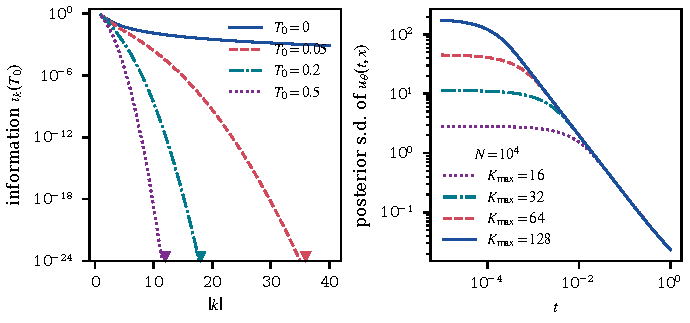
\includegraphics[width=\textwidth]{mf_heat}
\caption{Left: per mode information $\iota_k(T_0)$ from \eqref{m:eq:iota} for the two dimensional heat (Stokes) equation, $\nu=0.01$, $T=1$, for four observation start times; a triangle marks where a curve falls below $10^{-24}$ and leaves the frame. Right: posterior standard deviation of $u_\theta(t,x)$ at a fixed point, $\sqrt{\sum_{0<|k|\le K_{\max}}e^{-2\nu\lambda_kt}/(N\iota_k)}$ with $\iota_k=\iota_k(0)$, as a function of $t$ for $N=10^4$ and four truncations, $K_{\max}=16,32,64,128$. The $1/\sqrt N$ scaling is exact. At each fixed truncation the sum is finite at $t=0$ and the curve ends in a plateau, which rises by a factor close to four each time $K_{\max}$ doubles and so grows without bound with the truncation: this divergence as $t\to0$ is the failure of the supremum norm Bernstein von Mises theorem at the initial time. For larger $t$ the curves coincide, and the finiteness of the sum there whatever the truncation is parabolic smoothing.}\label{m:fig:heat}
\end{figure}

\begin{proposition}[Gram concentration and the finite $N$ Bernstein von Mises error]\label{m:prop:gram}
Let $\Phi$ be the design matrix \eqref{m:eq:design} for the heat equation with $D$ modes, uniform design on $[0,T]\times\T^d$, and $\norm{e_j}_\infty\le\sqrt2$, and let $N\ge D\log D$. Then, with the absolute constant $c=12$,
\[
\begin{gathered}
\Big\|\frac1N\Phi^\top\Phi-\diag(\iota_j)\Big\|_{op}\le c\,\sqrt{\frac{D\log D}{N}}\\
\text{with probability at least }1-D^{-1},
\end{gathered}
\]
and consequently, if $c\sqrt{D\log D/N}<\min_j\iota_j$, for the exact posterior covariance $V_N=(\Phi^\top\Phi+\Sigma_0^{-1})^{-1}$ and its Bernstein von Mises prediction $\bar V_N=(N\diag(\iota_j)+\Sigma_0^{-1})^{-1}$,
\[
\begin{gathered}
\norm{NV_N-N\bar V_N}_{op}\le\frac{c\sqrt{D\log D/N}}{\min_j\iota_j\,(\min_j\iota_j-c\sqrt{D\log D/N})}\\
\text{on the same event.}
\end{gathered}
\]
\end{proposition}

\begin{proof}
$\frac1N\Phi^\top\Phi=\frac1N\sum_i\phi_i\phi_i^\top$ with $\phi_i=(s_j(t_i)e_j(x_i))_j$ i.i.d., $E\phi_i\phi_i^\top=\diag(\iota_j)$ by orthonormality of $(e_j)$ and \eqref{m:eq:iota}, and $\norm{\phi_i}^2\le2D$. The matrix Bernstein inequality~\cite[Theorem 6.1.1]{tropp2015}, applied to the centered summands $(\phi_i\phi_i^\top-\diag(\iota_j))/N$, whose operator norms are at most $L=4D/N$ and whose variance proxy is at most $v=2D\max_j\iota_j/N\le2D/N$, bounds the probability that $\norm{N^{-1}\Phi^\top\Phi-\diag(\iota_j)}_{op}\ge t$ by $2D\exp\{-(t^2/2)/(v+Lt/3)\}$. At $t=\frac23\ell L+\sqrt{2\ell v}$ with $\ell=\log(2D^2)$ the exponent is at least $\ell$, so this probability is at most $D^{-1}$. For $D\ge2$, $\ell\le3\log D$, hence $t\le8D\log D/N+\sqrt{12D\log D/N}\le(8+\sqrt{12})\sqrt{D\log D/N}<12\sqrt{D\log D/N}$, where the middle step uses $D\log D/N\le1$; for $D=1$ the probability claimed is $0$ and there is nothing to prove. The second follows from the resolvent identity $NV_N-N\bar V_N=N\bar V_N(N\diag\iota-\Phi^\top\Phi)V_N$ and $\norm{N\bar V_N}_{op}\le1/\min_j\iota_j$, $\norm{NV_N}_{op}\le(\min_j\iota_j-c\sqrt{D\log D/N})^{-1}$.
\end{proof}

Since $\min_{j\le D}\iota_j\asymp D^{-2/d}$ by \eqref{m:eq:iota}, the relative error of the Bernstein von Mises covariance is $O(D^{2/d}\sqrt{D\log D/N})$, which is small exactly when $D\ll N^{d/(d+4)}$ up to logarithms. This is a quantitative counterpart, for the linear problem, of the dimension $J_N\asymp N^{d/(2\gamma+d)}$ of the projection $p_N$ in Nickl's centering \eqref{m:eq:thetahat} (his prior \eqref{m:eq:prior} is not truncated, and Condition~1 of Nickl~\cite{nicklbvm2024} imposes no dimension constraint).

\subsubsection{The Bernstein von Mises theorem, checked at finite $N$} Theorem~\ref{m:thm:nickl2} predicts that the posterior on mode $j$ is asymptotically $N(\tilde\theta_j,\sigma_j^2/N)$ with $\sigma_j^2=1/\iota_j$, and more precisely, keeping the prior term, with variance $(N\iota_j+\rho^{-2}\lambda_j^\alpha)^{-1}$. Figure~\ref{m:fig:heatgbc} compares this with the exact posterior from \eqref{m:eq:linpost} for the fixed truth $\theta_{0,k}=(1+k^2)^{-1}\mathrm{sign}(\sin k)$: the maximal relative discrepancy between the exact and the asymptotic standard deviation is $1.4\times10^{-4}$. The limit $\Ncal_{\theta_0}$ has variance $\sigma_j^2\asymp2\nu\lambda_jT$ growing with $j$, so $\sum_j\lambda_j^{-a}\sigma_j^2<\infty$ exactly when $a>1+d/2$, which is the tightness range of Proposition~2 of Nickl~\cite{nicklbvm2024}; the Gaussian limit is white noise roughened by $(-\Delta)^{1/2}$, and lives in $H^{-a}$ but not in $L^2$.

\begin{figure}[tp]\centering
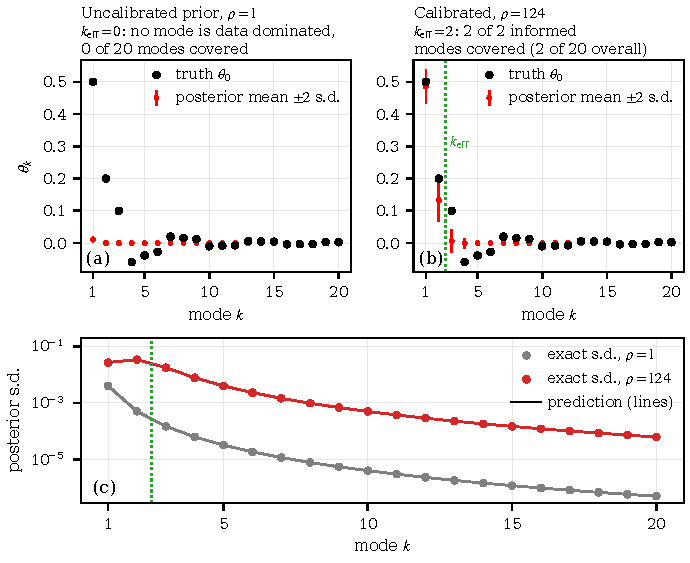
\includegraphics[width=\textwidth]{mf_heat_gbc}
\caption{Heat equation on $\T^1$, $N=2000$ observations, $K_{\max}=20$, $\alpha=3$, $\nu=0.01$, with the exact posterior of \eqref{m:eq:linpost}. Panel (a): the uncalibrated prior, $\rho=1$. No mode is data dominated, $k_{\rm eff}=0$; the truth lies up to $4949$ prior standard deviations from the prior mean and outside a two standard deviation credible interval in all $20$ modes. Panel (b): the same data with $\rho$ calibrated so that the prior standard deviation at $|k|=1$ matches the initial condition, $\rho=124$. Now $k_{\rm eff}=2$, and the truth lies inside the interval in every informed mode, with largest standardized error $1.96$. Panel (c): exact posterior standard deviation per mode in both settings against the prediction $(N\iota_k+\rho^{-2}\lambda_k^\alpha)^{-1/2}$ (lines). The agreement is close in both, which is why it validates nothing for $\rho=1$. Section~\ref{m:sec:expfinite} gives the diagnosis and Section~\ref{m:sec:covstudy} the coverage over replicates.}\label{m:fig:heatgbc}
\end{figure}

\subsubsection{Forward simulation and the trajectory theorem} Pushing the posterior through the heat flow gives $u_\theta(t,x)\mid Z\sim N\big(\sum_je^{-\nu\lambda_jt}\tilde\theta_je_j(x),\ \sum_{j,l}e^{-\nu(\lambda_j+\lambda_l)t}(V_N)_{jl}e_j(x)e_l(x)\big)$. Keeping only the diagonal terms, which is justified asymptotically because $\frac1N\Phi^\top\Phi$ concentrates on $\diag(\iota_j)$ by Proposition~\ref{m:prop:gram}, the posterior standard deviation of the state at time $t$ is, asymptotically, $N^{-1/2}\big(\sum_je^{-2\nu\lambda_jt}\sigma_j^2e_j(x)^2\big)^{1/2}$. Since $\sigma_j^2\asymp\lambda_j$, the series $\sum_j\lambda_je^{-2\nu\lambda_jt}$ converges for every $t>0$ and diverges at $t=0$: the trajectory is $\sqrt N$ estimable in supremum norm at every positive time, and the initial condition is not. Figure~\ref{m:fig:heat}(right) shows this, which is Theorem~\ref{m:thm:nickl1} and Remark~3 of Nickl~\cite{nicklbvm2024} in one picture; it is also Corollary~\ref{m:cor:commute}, since for a linear equation solve then simulate and simulate the limit are the same operation.

\subsubsection{GBC for the heat equation} Algorithm~\ref{m:alg:gbc} with the preconditioned summary $\tilde S_N=V_N\Phi^\top Y$ of Proposition~\ref{m:prop:linsuff} and an identity plus scale generator is exact. The learning problem has $D$ slopes (all equal to one), $D$ intercepts (all zero) and a $D\times D$ scale; with the prior diagonal and the Gram matrix asymptotically diagonal, the scale is asymptotically diagonal with entries $(N\iota_j+\rho^{-2}\lambda_j^\alpha)^{-1/2}$, so a generator with an identity skip, which fixes the slopes, and $2D$ free parameters, the intercepts and the diagonal of the scale, suffices, and $M\gg D$ simulations estimate it. This is the baseline against which the nonlinear case should be measured: the cost of nonlinearity is exactly the cost of the compact perturbation $\Kcal$ in \eqref{m:eq:fredholm}.

\subsection{The resolution the data support}\label{m:sec:resolution}

Four truncation dimensions appear in this part and they are different objects, so we fix them here once, in Table~\ref{m:tab:dims}.

\begin{table}[t]\centering\small
\caption{The four truncation dimensions, with the values they take in the computations of this part. The last column reports what is actually used, over $N=10^3$ to $1.3\times10^6$ where a range is given.}\label{m:tab:dims}
\begin{tabular}{@{}l>{\raggedright\arraybackslash}p{1.35in}>{\raggedright\arraybackslash}p{1.5in}l@{}}
\toprule
Symbol & What it is & Set by & Here\\
\midrule
$J_N$ & summary dimension the theory licenses & $N^{d/(2\gamma+d)}$, Theorem~\ref{m:thm:nickl2} & $2$ to $3$\\
$k_{\rm eff}$ & highest mode the data dominate the prior on & $N\iota_k\ge\rho^{-2}\lambda_k^\alpha$ & $0$ to $5$\\
$K_{\max}$ & modes retained in a computation & the user, $\ge k_{\rm eff}$ & $8$ to $128$\\
$D$ & coefficients the generator outputs & $\#\{|k|\le K_{\max}\}$ & $6$ to $20$\\
\bottomrule
\end{tabular}
\end{table}

\noindent Only $J_N$, and for the heat equation $D$ (Proposition~\ref{m:prop:regfixed}), carry asymptotic guarantees; $k_{\rm eff}$ is a property of the experiment and of the prior, computed in \eqref{m:eq:jeffdata} below and reported for each run in Section~\ref{m:sec:experiments}; $K_{\max}$ and $D$ are choices, and the rest of this subsection argues that taking them well above $J_N$ costs nothing and is what one should do. The $k_{\rm eff}$ range is $0$ at the uncalibrated prior of Figure~\ref{m:fig:heatgbc} and $2$ to $5$ at the calibrated one, whose $K_{\max}$ is $20$; Section~\ref{m:sec:expstudy} has $K_{\max}=D=8$ and Section~\ref{m:sec:expns} has $D=6$, and the analytic computation of Figure~\ref{m:fig:heat}(right) takes $K_{\max}$ from $16$ to $128$.

The theory licenses a summary of dimension $J_N\asymp N^{d/(2\gamma+d)}$. With the regularity $\gamma>12$ that Konen and Nickl~\cite{konennickl2026} require and $d=2$ this is at most $N^{1/13}$, its value at $\gamma=12$: at most $1.7$ modes at $N=10^3$, $2.9$ at $N=10^6$, $5.9$ at $N=10^{10}$. Table~\ref{m:tab:iota} tabulates $\iota_j$ to $|k|=32$ and Figure~\ref{m:fig:heat} plots to $|k|=40$.

Ask independently how many modes the data inform, with no reference to the asymptotic theory. A mode is informed when its data precision exceeds its prior precision, $N\iota_k\ge\rho^{-2}\lambda_k^\alpha$. Using $\iota_k=(1-e^{-2\nu\lambda_kT})/(2\nu\lambda_kT)\sim(2\nu\lambda_kT)^{-1}$ for $\nu\lambda_kT\gg1$, the crossover sits at $\lambda_K=(N\rho^2/2\nu T)^{1/(\alpha+1)}$, and since $\#\{k:\lambda_k\le\Lambda\}\asymp\Lambda^{d/2}$ the number of informed modes is
\begin{equation}\label{m:eq:jeffdata}
J^{\rm data}_N\asymp\Big(\frac{N\rho^2}{2\nu T}\Big)^{d/(2(\alpha+1))}.
\end{equation}
The fixed prior of Section~\ref{m:sec:heat} has covariance eigenvalues $\rho^2\lambda_j^{-\alpha}$ on the modes with $|k|\le K_{\max}$, and the series it truncates has reproducing kernel Hilbert space (RKHS) $H^\alpha_0$, the RKHS of \eqref{m:eq:prior} when $\gamma=\alpha$; under \eqref{m:eq:prior} itself, whose scale $\rho^2=1/(N\delta_N^2)$ shrinks with $N$, the informed count is instead $J^{\rm eff}_N=o(J_N)$ (Proposition~\ref{m:prop:pr} and Remark~\ref{m:rem:jeff}). Comparing exponents,
\[
\frac{d}{2\gamma+d}\quad\text{against}\quad\frac{d}{2(\alpha+1)},
\]
which are equal precisely when $2(\alpha+1)=2\alpha+d$, that is when $d=2$, the case the framework is built for. In $d=1$ and $d=3$ the exponents differ, but only slightly: $1/7$ against $1/8$ and $1/3$ against $3/8$ at $\alpha=\gamma=3$, so that, constants aside, the two dimensions differ by the slowly growing factors $N^{1/56}$ and $N^{1/24}$, and the numerical gap over seven decades of $N$ is a factor between $1.1$ and $2.6$. Solving $N\iota_k=\rho^{-2}\lambda_k^\alpha$ numerically for $d=1$, $\alpha=3$, with $\rho$ calibrated so the prior standard deviation at $k=1$ matches the initial condition, gives $J^{\rm data}_N=2,2,3,4,6,8,11,15$ at $N=10^3,\dots,10^{10}$ and a fitted exponent of $0.134$ against the $0.125$ that \eqref{m:eq:jeffdata} predicts; the excess is the integer rounding of a mode count, which biases the slope upward at small counts. Read the other way, seven decades of data buy a factor of $7.5$ in resolution.

So $J_N$ is not a conservative artifact of the proof. It is the number of modes the experiment resolves, and any procedure that respects this prior, on this observation model, resolves the same number. What makes it small is the regularity the framework demands: $\gamma>12$ is a very smooth prior, and a very smooth prior leaves few modes in which the data outweigh it. Relaxing that regularity requirement, which is open, would raise the licensed and the achievable resolution together.

Table~\ref{m:tab:iota} and Figure~\ref{m:fig:heat} tabulate $\iota_j$ over a wide band because $\iota_j$ is a property of the forward operator, defined at every mode and worth displaying precisely to show how fast the barrier bites; they are not claims that those modes are estimable. And the grid on which the forward solve is carried out is a fifth quantity, not one of the four: it must resolve the dynamics rather than the estimand, and is far finer than $K_{\max}$ demands. Where a statement concerns estimability we write $J_N$; where it concerns what the generator outputs we write $D$.

\subsubsection{Which constraint binds} Two questions follow from a $J_N$ this small. First, what the method delivers beyond a Laplace approximation in a handful of modes: at $N=80$, the sample size of the Navier Stokes run, nothing on accuracy (Section~\ref{m:sec:expns}). What is delivered is amortization and simulation only access to the forward map. Second, whether $J_N$ is ever large enough for the condition $M\gg J_N$ of Theorem~\ref{m:thm:qnnA}, which Corollary~\ref{m:cor:locG}(ii) carries over at every localization radius, to bind before $D$ does. Here it is not, by a wide margin: $J_N$ lies between $2$ and $6$, while the experiments use $M$ between $250$ and $32000$, a budget set by the term $a_v\asymp D/M$ of \eqref{m:eq:decomp} and not by $J_N$ at all. For $M=1200$, a value in that range, to bind one needs $J_N\approx1200$, which at $d=2$, $\gamma=12$ arrives at $N\approx10^{40}$. The condition is vacuous under this prior, not vacuous in general: at the $\gamma=3$ Schauder theory is expected to permit (Open Question~\ref{m:op:unif}) the same $J_N$ arrives at $N\approx2\times10^{12}$. Relaxing the regularity requirement is what would make the simulation budget, rather than the dissipation barrier, the thing that limits resolution.

\section{Worked example: two dimensional Navier Stokes}\label{m:sec:ns}

Consider the periodic two dimensional system in the form of Konen and Nickl~\cite{konennickl2026},
\begin{equation}\label{m:eq:nsproj}
\frac{du}{dt}+\nu Au+B[u,u]=f,\qquad u(0)=\theta\in\Hds{\alpha},
\end{equation}
with $A=-\Delta$ on divergence free mean zero fields, whose eigenfunctions are $e_j(x)=c_jh_{k_j}(x)$, $c_j=(-k_{j,2},k_{j,1})/|k_j|$, $h_k=e^{2\pi ik\cdot x}$, with eigenvalues $\lambda_j=4\pi^2|k_j|^2$; one degree of freedom per wavevector because of incompressibility. Two conventions for the torus are used from here on and no formula mixes them: the unit torus, where $\lambda_k=4\pi^2|k|^2$, for the Stokes limit and Figure~\ref{m:fig:tg}, as for the heat equation of Section~\ref{m:sec:heat} and the Schr\"odinger equation of Section~\ref{m:sec:nondiss}, and the $2\pi$ periodic torus, where $\lambda_k=|k|^2$, for the Taylor Green vortex, Remark~\ref{m:rem:advection} and the experiment of Section~\ref{m:sec:expns}; Section~\ref{m:sec:tg} converts between them.

\subsection{The Stokes limit and the linearization}

If $\theta_0=0$ and $f=0$ then $u_{\theta_0}\equiv0$, the linearized equation \eqref{m:eq:tangentgen} is the Stokes equation $\partial_tU+\nu AU=0$, $\I_{\theta_0}=\Lcal$, $\Kcal=0$ in \eqref{m:eq:fredholm}, and Section~\ref{m:sec:heat} applies verbatim with the divergence free basis: the sufficient statistic is the adjoint Stokes flow of the data, the information per mode is \eqref{m:eq:iota}, the Bernstein von Mises covariance is $T(\I^*\I)^{-1}$ with diagonal $1/\iota_j=2\nu\lambda_jT/(1-e^{-2\nu\lambda_jT})$, and the limit $\Ncal_{\theta_0}$ is tight on $\Hds{-\beta}$ for $\beta>2$ (Proposition~2.7 of Konen and Nickl~\cite{konennickl2026}). The RKHS of the limit is $\Hds{-1}$ because $\sigma_j^2\asymp\lambda_j$ means the covariance operator is $\asymp(-\Delta)$, whose RKHS norm is $\norm{\cdot}_{\dot H^{-1}}$.

\subsubsection{The Taylor Green background} To see the nonlinearity we need a background flow about which the linearized equation is tractable. The Taylor Green vortex~\cite{taylorgreen1937} of \eqref{m:eq:tg} below, on the $2\pi$ periodic torus, is an exact solution of \eqref{m:eq:nsproj} with $f=0$, because $(u\cdot\nabla)u$ is a gradient and is absorbed into the pressure; it has wavevectors $(\pm1,\pm1)$ only, and decays at the Stokes rate of its own mode. On this torus $\lambda_k=|k|^2$, so that the mode $(1,1)$ decays at the rate $2\nu$. Take $\theta_0=u_{\rm TG}(0)$ as the true initial condition. The equation linearized at a background $u_\vartheta$ is
\begin{equation}\label{m:eq:tangentgen}
\partial_tU+\nu AU+B[u_\vartheta,U]+B[U,u_\vartheta]=0,\qquad U(0)=h,
\end{equation}
and because $u_{\rm TG}$ has four Fourier modes, $B[u_{\rm TG},\cdot]+B[\cdot,u_{\rm TG}]$ couples wavevector $k$ only to $k\pm(1,\pm1)$. Section~\ref{m:sec:tg} computes that coupling explicitly. The tangent operator is the Stokes diagonal $-\nu|k|^2$ plus a sparse skew coupling to the four diagonal neighbors whose row sum is $\asymp A|k|$, and Remark~\ref{m:rem:advection} measures the ratio of this coupling to the viscous decay.

\begin{remark}[The advection to dissipation ratio, with constants]\label{m:rem:advection}
Form the Jacobian of the vorticity right hand side at $u_{\rm TG}(0)$ on the $2\pi$ torus, where $\lambda_k=|k|^2$, and compare shell by shell the off diagonal row sum of moduli against the diagonal $\nu|k|^2$. The four Taylor Green coefficients have components of modulus $A/4$ and are orthogonal to their own wavevectors, so the transport term $(u_{\rm TG}\cdot\nabla)$ contributes $cA|k|$ to the row sum with $c$ near one, while the stretching term contributes $O(A)$ and is negligible past the first few shells. Measured at $n=48$, $\nu=0.01$, $A=1$, the row sum is $cA|k|$ with $c$ between 0.74 and 0.98 (the 10th and 90th percentiles) over $6\le|k|\le n/3$, median 0.91, so
\[
\frac{\text{advective coupling at }k}{\text{viscous decay at }k}=\frac{cA}{\nu|k|},\qquad
c\approx0.91 .
\]
The measured ratio is 6.2 at $|k|=16$, against 5.7 from this formula; the formula crosses one at $|k|\approx91$ and reaches a tenth only near $|k|\approx910$. Two things follow. The $1/|k|$ decay is what makes $\Kcal$ in \eqref{m:eq:fredholm} compact, so the Fredholm decomposition is meaningful. But the constant $A/\nu$ is large, so at this viscosity the nonlinear correction to the Stokes information operator is of order one across every mode the truncation of Section~\ref{m:sec:expns} resolves: there the Stokes limit is a structural guide, not a numerical approximation. Computed by \texttt{ns/advection\_ratio.py}.
\end{remark}

\subsection{The explicit Taylor Green coupling}\label{m:sec:tg}

The Taylor Green vortex
\begin{equation}\label{m:eq:tg}
u_{\rm TG}(t,x)=A\,e^{-2\nu t}\big(\sin x_1\cos x_2,\ -\cos x_1\sin x_2\big)
\end{equation}
on the $2\pi$ periodic torus has the four Fourier coefficients $\hat u_\ell$, $\ell\in\{(\pm1,\pm1)\}$, each with components of modulus $Ae^{-2\nu t}/4$. With $\widehat{(u\cdot\nabla)v}_k=\sum_{\ell+m=k}i\,(\hat u_\ell\cdot m)\,\hat v_m$ and $P_k=\Id-kk^\top/|k|^2$ the Leray projector in Fourier space, the linear operator in \eqref{m:eq:tangentgen} at $u_\vartheta=u_{\rm TG}$ is
\begin{equation}\label{m:eq:tgcoupling}
\begin{split}
\widehat{\big(B[u_{\rm TG},U]+B[U,u_{\rm TG}]\big)}_k={}&i\,P_k\sum_{\ell\in\{(\pm1,\pm1)\}}\Big[(\hat u_\ell\cdot(k-\ell))\,\hat U_{k-\ell}\\
&\qquad+(\hat U_{k-\ell}\cdot\ell)\,\hat u_\ell\Big].
\end{split}
\end{equation}
Both terms are bounded by $A|k|e^{-2\nu t}|\hat U_{k-\ell}|$ up to a constant, so in the divergence free basis mode $k$ evolves by $-\nu|k|^2\hat U_k$ plus terms of size $A|k|e^{-2\nu t}$ times $\hat U_{k\pm(1,\pm1)}$, so that on this torus the ratio of advective coupling to viscous decay is $\asymp A/(\nu|k|)$. On the unit torus $[0,1]^2$ the same vortex is $Ae^{-8\pi^2\nu t}(\sin2\pi x_1\cos2\pi x_2,\ -\cos2\pi x_1\sin2\pi x_2)$, with $\lambda_k=4\pi^2|k|^2$, and every derivative in the coupling carries a factor $2\pi$, so that the ratio is $2\pi A|k|/(\nu\lambda_k)\asymp A/(2\pi\nu|k|)$; this is the form plotted in Figure~\ref{m:fig:tg}.

\begin{figure}[tp]\centering
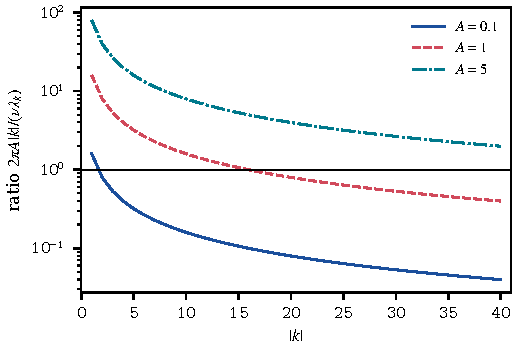
\includegraphics[width=0.75\textwidth]{mf_tg}
\caption{Ratio of advective coupling to viscous decay, $2\pi A|k|/(\nu\lambda_k)$ with $\lambda_k=4\pi^2|k|^2$ (the unit torus), for the linearized Navier Stokes equation about the Taylor Green vortex of amplitude $A$, $\nu=0.01$; the horizontal line marks one. Where the ratio exceeds one the nonlinear correction $\Kcal$ to the Stokes information operator matters; where it is small the Stokes formulas of Section~\ref{m:sec:heat} govern the posterior. The crossover scale grows linearly in $A/\nu$.}\label{m:fig:tg}
\end{figure}

\subsection{The sufficient statistic and the pipeline}

Definition~\ref{m:def:summary} specializes as follows. Given a preliminary estimate $\bar\theta_N$ from one half of the data (for Taylor Green, a few mode least squares fit of its early observations), compute, on the observations of the other half:
\begin{enumerate}[nosep]
\item the nonlinear forward solve $u_{\bar\theta_N}$ on $[0,T]$ by a pseudospectral method, and the residuals $r_i=Y_i-u_{\bar\theta_N}(t_i,x_i)$;
\item the adjoint linearized solve: $w$ solves, backward in time,
\[
\begin{split}
-\partial_sw+\nu Aw+{}&B[u_{\bar\theta_N},\cdot]^*w+B[\cdot,u_{\bar\theta_N}]^*w\\
&=\sum_ir_i\,\delta_{x_i}\delta_{t_i},\qquad w(T)=0,
\end{split}
\]
where the adjoints of the advection terms are, by Proposition~3.1(i) of Konen and Nickl~\cite{konennickl2026} and a direct computation, $B[u,\cdot]^*w=-B[u,w]$, which uses $\nabla\cdot u=0$ and periodicity, and $B[\cdot,u]^*w=P[(\nabla u)^\top w]$, in which $\nabla u$ is the Jacobian $(\nabla u)_{ij}=\partial_ju_i$, so that $\big((\nabla u)^\top w\big)_j=\sum_i w_i\partial_ju_i$; then $\I^*_{\bar\theta_N}r=w(0)$;
\item the application of $(F_N+\Sigma_0^{-1})^{-1}$, with $F_N$ the realized information of Remark~\ref{m:rem:reg}, by conjugate gradients (CG) preconditioned with the explicit Stokes inverse $2\nu(-\Delta)(\Id-S_{2T})^{-1}$ from \eqref{m:eq:fredholm}, each iteration costing one tangent solve and one adjoint solve.
\end{enumerate}
The output is \eqref{m:eq:regsummary}, the summary we compute (Remark~\ref{m:rem:reg}); with $(\I^*_{\bar\theta_N}\I_{\bar\theta_N})^{-1}$ in step 3 and $p_N$ applied to $w(0)$ before it, it is \eqref{m:eq:onestep} for one fold, and its average over the two folds, projected onto the first $J_N$ Stokes modes, is the summary $\hat S_N$ of Definition~\ref{m:def:summary}. Steps 1 and 2 are one gradient evaluation of 4DVar, and step 3 is a Gauss Newton solve. The GBC generator then learns the map from the summary to posterior draws, which by Remark~\ref{m:rem:affine} is asymptotically the identity plus the scale $T(\I^*\I)^{-1}/N$, whose diagonal is the Stokes scale of Table~\ref{m:tab:iota} corrected by the Taylor Green coupling at low $|k|$.

\subsubsection{What Konen Nickl's theorem says for this example} With $\alpha>12$, $\theta_0=u_{\rm TG}(0)$ smooth, and $T_0=0$: the posterior on $\theta$ is asymptotically $N(\tilde\theta_N,T(\I^*_{\theta_0}\I_{\theta_0})^{-1}/N)$ in $\Hds{-\sigma}$, $\sigma>9$; the posterior on $u_\theta(t)$ for $t\in[t_{\min},t_{\max}]$ is asymptotically the Gaussian field solving \eqref{m:eq:tangentgen} with initial datum from that law, at rate $1/\sqrt N$ in supremum norm; a credible band of posterior probability $1-\beta$ around $u_{\tilde\theta_N}$ has frequentist coverage $\to1-\beta$; and no estimator does better in local asymptotic minimax sense. The Taylor Green structure lets one see the covariance: it is the Stokes covariance on the diagonal, modified at $|k|\lesssim A/(2\pi\nu)$ on the unit torus (at $|k|\lesssim A/\nu$ on the $2\pi$ torus) by the nearest neighbor coupling, and the modification is a compact operator so it does not change the tightness range or the RKHS. For the advection functional $\Phi_t(u)=(u\cdot\nabla)u$ at time $t$, the delta method of Section~2.4 of Konen and Nickl~\cite{konennickl2026} gives a $\sqrt N$ Gaussian limit for $\Phi_t(u_{\tilde\theta_N})$, and for Taylor Green $\Phi_t(u_{\rm TG})$ is a gradient field, so the limit describes the fluctuation of the pressure gradient.

\subsubsection{The pipeline} The Navier Stokes pipeline is: pseudospectral simulations from a localized proposal (Step 1 of Algorithm~\ref{m:alg:gbc}, as amended in Algorithm~\ref{m:alg:loc}); per simulated data set, the summary \eqref{m:eq:regsummary} computed above; an identity skip quantile network with a learned scale (Step 2); evaluation at the observed summary (Step 3); forward simulation of the draws (Step 4), or by Corollary~\ref{m:cor:commute} simulation of the tangent equation from the Gaussian limit. With observations on $[T_0,T]$, $T_0>0$, Table~\ref{m:tab:iota} says which modes are lost; the pipeline is unchanged, and the scale learned in Step 2 becomes enormous for $|k|\gtrsim(\nu T_0)^{-1/2}$, which is correct.

\subsection{What survives a realistic design}\label{m:sec:designrobust}

The design in \eqref{m:eq:model} is $N$ points drawn independently and uniformly on $[0,T]\times\Omega$. Real observing systems are not that: they are fixed stations, satellite swaths on repeat orbits, radiosondes at synoptic hours, with errors correlated in space and between channels, and with observation operators, radiances or column integrals, that are not point evaluations.

\emph{Design robust.} Everything that holds for an arbitrary set of design points or depends on the design only through its information operator. Let $\varpi$ be any probability measure on $[0,T]\times\Omega$ and define $\langle h,\I^*_\varpi\I_\varpi h\rangle=\int|\I_\theta h|^2\,d\varpi$, which for the uniform design of \eqref{m:eq:model} is $T^{-1}\langle h,\I^*\I h\rangle$. Lemma~\ref{m:lem:adjoint}, Proposition~\ref{m:prop:linsuff}, Lemma~\ref{m:lem:exact} and Theorem~\ref{m:thm:gap} hold verbatim, and so does the first part of Theorem~\ref{m:thm:locbias}, the mean and variance \eqref{m:eq:varR} of the residual. The regularized summary of Remark~\ref{m:rem:reg} uses the realized information of the design actually drawn and needs no change, and Definition~\ref{m:def:summary} holds with $(\I^*_\varpi\I_\varpi)^{-1}$ in place of $T(\I^*\I)^{-1}$, given pilot estimators with the rates it asks for under $\varpi$. Theorem~\ref{m:thm:main} carries over once the Bernstein von Mises theorem and the conditions behind it are assumed to hold under $\varpi$ (Theorem~\ref{m:thm:nickl2} is proved for independent uniform times and points). Proposition~\ref{m:prop:radius} carries over once Conditions 2A to 2D hold with $\varpi$ in place of the uniform measure and the per coordinate form of Theorem~\ref{m:thm:locbias}, on which its term $\beta(c)$ rests, is available; that form needs the information operator to commute with the prior covariance. For the heat and Stokes equations a design that is uniform in space at each time, whatever the law of the times, keeps $\I^*_\varpi\I_\varpi$ diagonal in $(e_j)$, with the per mode information $\int e^{-2\nu\lambda_jt}\,d\varpi$ in place of $\iota_j$; under a design that is not uniform in space $\I^*_\varpi\I_\varpi$ is in general not diagonal. Correlated errors are equally harmless: with noise covariance $\Sigma_\varepsilon$ in place of $\varsigma^2\Id$, replace $\I^*\I$ by $\I^*\Sigma_\varepsilon^{-1}\I$ throughout and the adjoint statistic by $\I^*\Sigma_\varepsilon^{-1}r$, one extra linear solve. Observation operators that are not point evaluations are the same statement: if observation $i$ reports $\langle A_iu,\cdot\rangle$ rather than $u(t_i,x_i)$, the adjoint is driven by $\sum_ir_iA_i^*$ in place of $\sum_ir_i\delta_{X_i}$.

\emph{Not design robust.} Three things use the i.i.d. uniform design itself. Proposition~\ref{m:prop:gram} is a matrix Bernstein bound and needs independent summands, as do the second moment bounds on the whitened Gram matrix behind Propositions~\ref{m:prop:regheat} and~\ref{m:prop:regfixed}; under a correlated or deterministic design each must be replaced by a bound for dependent or fixed designs, and the concentration of $\Phi^\top\Phi$ on $N\,\diag(\iota_j)$ that Remark~\ref{m:rem:reg} warns about is exactly what degrades. The closed forms $\iota_j=\tfrac1T\int_0^Te^{-2\nu\lambda_jt}dt$ of \eqref{m:eq:iota} and the numbers in Table~\ref{m:tab:iota} are the uniform design values and change under any other $\varpi$; a fixed station network, for instance, samples $\Omega$ on a lattice and aliases modes above its Nyquist frequency, which no amount of data repairs. And the identification of $J_N$ with $N\delta_N^2$ presumes the law of large numbers (LLN) limit of the uniform design; under a design that never visits part of $\Omega$, the relevant dimension is set by the reachable subspace instead.

The practical reading is that the method transfers and the numbers do not. An implementer should recompute $\I^*_\varpi\I_\varpi$ for the observing system at hand rather than reuse $\iota_j$, and should expect Remark~\ref{m:rem:reg}'s regularized summary to matter more, not less, since a realistic design is further from its LLN limit than a uniform one. Every experiment reported in Section~\ref{m:sec:experiments}, the Navier Stokes run included, uses the uniform design of \eqref{m:eq:model}.

\section{Experiments}\label{m:sec:experiments}

Everything reported here is produced from fixed seeds by scripts that are supplied, with their recorded outputs, as ancillary files of our paper~\cite{polsonsokolov2026manifold} and described in Appendix~\ref{app:code}. The generator \texttt{make\_experiments\_tex.py} wrote the experiments section of that paper, tables included, directly from the resulting \texttt{json}, so every measured number in the tables and in the figure comes from a recorded run rather than being transcribed by hand. The setting is the heat equation of Section~\ref{m:sec:heat} on $\Omega=[0,1]$ with $\nu=0.01$, $T=1$, the fixed prior of that section with $\alpha=3$, and the conjugate Gaussian posterior available in closed form, so that the exact posterior is known and every approximation can be measured against it rather than against another approximation.

\subsection{The finite $N$ check, in the regime where the data speak}\label{m:sec:expfinite}

Table~\ref{m:tab:diag} reports the diagnosis. The first row is the uncalibrated setting of panel (a) of Figure~\ref{m:fig:heatgbc}, $\rho=1$ and $N=2000$: no mode has data precision exceeding prior precision. The agreement with the Bernstein von Mises scale there, $1.43\times10^{-4}$, is therefore not a validation of anything: both sides of the comparison are the prior, and a diagnostic that compares the prior with itself is vacuous whatever number it returns.

Two things are wrong at once and they have to be separated. The first is the scale of the prior, which $\rho$ fixes: calibrating $\rho$ so that the prior standard deviation at $|k|=1$ matches the initial condition there gives $\rho=124.0$, moves $k_{\rm eff}$ from $0$ to 2, covers every informed mode, and brings the relative $L^2$ error to $0.257$. The second is the shape: the initial condition $\theta_{0,k}=(1+k^2)^{-1}\mathrm{sign}(\sin k)$ decays like $k^{-2}$ whereas a draw from the fixed prior with $\alpha=3$ decays like $k^{-3}$, so after calibration the worst mode is still $39.9$ prior standard deviations out. That tail is invisible while $k_{\rm eff}$ is small and becomes visible as $N$ grows: the informed modes covered go from 2 of 2 at $N=2\times10^3$ to 3 of 5 at $N=1.3\times10^6$, with the worst standardized error over informed modes rising to $7.91$. Nothing is wrong with the posterior; the prior is wrong about the truth, and more data is what reveals it.

The last three rows replace the fixed $\theta_0$ by a draw from the prior itself, the only setting in which nominal coverage is the right thing to expect. Relative $L^2$ error stays near one at the smaller two, which is not a failure: this draw is small, with norm $0.0208$ against a prior root mean square norm of $0.50$, and the posterior standard deviations of its informed modes are of the same size ($0.027$ and $0.034$ at $N=2\times10^3$), so the error of the posterior mean is of the size of the signal itself and a ratio above one can occur while every informed mode stays within $2.2$ posterior standard deviations. Section~\ref{m:sec:resolution} says how many modes the data can resolve.

\begin{table}[t]\centering\footnotesize\setlength{\tabcolsep}{3pt}
\caption{The finite $N$ check for the heat equation. $k_{\rm eff}$ is the number of modes with $N\iota_k\ge\rho^{-2}\lambda_k^\alpha$; ``truth/prior sd'' is $\max_k|\theta_{0,k}|/\sigma_{0,k}$, a measure of how atypical the truth is under the prior; the coverage columns count the modes whose truth lies within two posterior standard deviations, over the informed modes and over all twenty; with $k_{\rm eff}$ this small these are counts and not estimates of a coverage probability, for which see the replicate study of Section~\ref{m:sec:expstudy}; $|z|_{\max}$ is the largest standardized error over informed modes; and the last column is the largest relative discrepancy, over all twenty modes, between the exact posterior standard deviation and the Bernstein von Mises (BvM) scale with the prior precision added, $(N\iota_k+\sigma_{0,k}^{-2})^{-1/2}$. The truth of the last block is a fixed draw from the prior that is typical in each coordinate but small in norm.}\label{m:tab:diag}
\begin{tabular}{rrrrrrrrr}
\toprule
$N$ & $\rho$ & $k_{\rm eff}$ & \shortstack[r]{truth/\\prior sd} & \shortstack[r]{cov.\\inf.} & \shortstack[r]{cov.\\all} & $|z|_{\max}$ & \shortstack[r]{rel.\\$L^2$} & \shortstack[r]{BvM\\rel.}\\
\midrule
\multicolumn{9}{@{}l}{Uncalibrated prior}\\
$2\times10^3$ & 1 & 0 & 4948.6 & n/a & 0 of 20 & n/a & 0.982 & $1.43\times10^{-4}$ \\
\addlinespace
\multicolumn{9}{@{}l}{Calibrated $\rho$}\\
$2\times10^3$ & 124 & 2 & 39.9 & 2 of 2 & 2 of 20 & 1.96 & 0.257 & $6.05\times10^{-3}$ \\
$5\times10^4$ & 124 & 3 & 39.9 & 3 of 3 & 3 of 20 & 0.92 & 0.144 & $1.60\times10^{-3}$ \\
$1.3\times10^6$ & 124 & 5 & 39.9 & 3 of 5 & 3 of 20 & 7.91 & 0.081 & $7.77\times10^{-4}$ \\
\addlinespace
\multicolumn{9}{@{}l}{Fixed draw from the prior}\\
$2\times10^3$ & 124 & 2 & 1.9 & 2 of 2 & 20 of 20 & 0.59 & 1.007 & $6.05\times10^{-3}$ \\
$5\times10^4$ & 124 & 3 & 1.9 & 2 of 3 & 19 of 20 & 2.18 & 1.270 & $1.60\times10^{-3}$ \\
$1.3\times10^6$ & 124 & 5 & 1.9 & 5 of 5 & 20 of 20 & 1.54 & 0.250 & $7.77\times10^{-4}$ \\
\bottomrule
\end{tabular}
\end{table}

\subsection{Cost and accuracy against the alternatives}\label{m:sec:expcost}

Table~\ref{m:tab:cost} reports what one analysis costs. Unless a variant is named, GBC in this table and in the rest of this section is Algorithm~\ref{m:alg:loc} with $c=2$ and the identity head, applied to the regularized summary of Remark~\ref{m:rem:reg}. The units are forward or adjoint solves of the linearized equation, which is the currency in which data assimilation is priced, together with wall clock for the methods actually run here. The two comparators are the Laplace approximation at the posterior mode and the preconditioned Crank Nicolson sampler (pCN), in the form given by Cotter and coauthors~\cite{cotter2013}.

\begin{table}[t]\centering\footnotesize\setlength{\tabcolsep}{4pt}
\caption{Cost and accuracy for one analysis of the heat equation, $N=50000$, $|k|\le8$, single core. Errors are the maximum over the retained modes, in units of the exact posterior standard deviation (psd). ``Amortized'' records whether a second data set can be analyzed without repeating the cost. $\dagger$: analytic, not measured. In this linear Gaussian model both the Laplace approximation at the posterior mode and the GBC generator have the exact posterior mean, by Proposition~\ref{m:prop:linsuff}, so their mean error is exactly zero at every budget. The standard deviation ratio, the median over the retained modes of the reported posterior standard deviation divided by the exact one, is the column that carries information here. Neither the $8000$ solves of GBC, a forward and an adjoint solve for each of its $M=4000$ simulations, nor the $2$ of Laplace, one forward and one adjoint solve, include forming the Gauss Newton covariance $(\Phi^\top\Phi+\Sigma_0^{-1})^{-1}$, which is the covariance of the Laplace row and which GBC's localized proposal and summary also use. It is formed once in either method and takes one further linearized solve per retained mode, $8$ here; the Laplace time is that of forming it from $\Phi$, and the GBC time, which covers the simulations, the fit and the $4000$ draws, leaves it out.}\label{m:tab:cost}
\begin{tabular}{lrrrrl}
\toprule
Method & Solves & Time (s) & \shortstack[r]{Max err.\\(psd)} & \shortstack[r]{sd\\ratio} & Amortized\\
\midrule
GBC, Algorithm~\ref{m:alg:loc}, $c=2$ & 8000 & 2.91 & $0^{\dagger}$ & 1.003 & amortized \\
Laplace at $\hat S_N$ & 2 & 0.0003 & $0^{\dagger}$ & $1^{\dagger}$ & no \\
pCN, $2\times10^{5}$ iterations & 200000 & 86.5 & 0.325 & 0.947 & no \\
\bottomrule
\end{tabular}
\end{table}

Three readings. First, GBC is not more accurate than Laplace and cannot be: by Definition~\ref{m:def:gen} its generator is a Monte Carlo estimate of the Laplace approximation, so its mean is that approximation's mean exactly, and the $0.016$ posterior standard deviations one reads off the worst of its $4000$ output draws is the sampling error of those draws, not an error of the method. What it buys over Laplace is that the forward map is reached only by simulation and that no Hessian is evaluated at the training draws: the one Gauss Newton covariance of Algorithm~\ref{m:alg:loc} is formed once, at the preliminary estimate (Remark~\ref{m:rem:whichcov}). Second, pCN is included to exhibit the Monte Carlo rate the two methods share, not as a tuned competitor: in this conjugate model the exact posterior is a known Gaussian that can be sampled directly and a whitened or Gibbs sampler would mix in one step, so the comparison is not in GBC's favor on a single data set: $200000$ iterations and a tuned acceptance rate of 0.246 at $\beta=0.0491$ deliver a minimum effective sample size of 16 across the retained modes, which is why its worst mode error is larger than GBC's and is Monte Carlo noise rather than bias: its posterior standard deviation ratio is 0.947. Given enough iterations pCN is exact and GBC is not. Third, the cost that matters operationally is the ratio to a 4DVar minimization. Neither 4DVar nor an ensemble Kalman filter (EnKF) is run here: a 4DVar minimization returns a point estimate, and an ensemble filter returns an ensemble that is a posterior sample only for a linear forward map and a large ensemble, so no error in these units is reported for either. Both do have conventional solve counts: 20 for a Gauss Newton 4DVar at ten inner iterations of one forward and one adjoint solve, and one solve per ensemble member for an ensemble filter. Against those conventions one GBC analysis is 400 4DVar equivalents at $M=4000$ and 80 times a 100 member EnKF. Those are the numbers Section~\ref{m:sec:related} refers to, and they are the price of amortization: the 4000 simulations are spent once, and every subsequent data set is a forward pass.

\subsection{Error against cost, and coverage over replicates}\label{m:sec:expstudy}

The error against cost and the coverage over replicates are both studied at $N=50000$ with $D=8$ modes retained, of which $k_{\rm eff}=3$ are data dominated, and at the calibrated $\rho=124$ of Section~\ref{m:sec:expfinite}. A single realization cannot separate a miscalibrated posterior from an unlucky draw, so calibration is checked over replicates, on three truth arms. The result, set out in Section~\ref{m:sec:covstudy} and shown for the arm drawn from the prior in the lower panel of Figure~\ref{m:fig:cost}, is that GBC reproduces whatever the exact posterior does, on every arm, under a paired McNemar test that takes the replicate as its unit.

In the linear Gaussian model of Section~\ref{m:sec:heat} Proposition~\ref{m:prop:linsuff} gives the mean map in closed form, so GBC's posterior mean is exact at every budget and only the $D\times D$ covariance is estimated from the $M$ simulations. Scoring the mean therefore measures nothing about the method: over 40 replicates and 8 budgets, 320 measurements in all, its error is exactly zero (Remark~\ref{m:rem:artifact}).

\begin{remark}[Why a finite draw mean error is not an approximation floor]\label{m:rem:artifact}
Scoring GBC's posterior mean against the exact one in this model measures a quantity whose value is exactly zero, so any nonzero reading is the sampling noise of however many output draws were taken. Holding that count fixed at 4000 while the simulation budget sweeps a factor of 128 returns 0.023 to 0.044 posterior standard deviations with a fitted slope against the budget of $-0.029$, flat. That flatness is not an approximation floor of the plug in generator. The quantity decays in the number of output draws, not in $M$, so no simulation budget can move it and there is nothing there to converge. A Gaussian head does carry a genuine approximation error wherever the posterior is not Gaussian, but a linear Gaussian benchmark is precisely the case in which that error vanishes identically, so this diagnostic cannot measure it at any budget. Any study of a Gaussian head generator that scores the mean on a conjugate benchmark meets the same trap.
\end{remark}

What the simulations buy is the covariance, and scored analytically it converges at the Monte Carlo rate with no floor. Across the 3 generator variants and both covariance metrics the fitted slope of $\log$ error against $\log$ solves lies between $-0.521$ and $-0.495$ against a nominal $-1/2$, with replicate standard error 0.009; raising $M$ from 250 to 32000 cuts the error on the standard deviations from 0.081 to 0.0071. The learned mean variant, which ignores Proposition~\ref{m:prop:linsuff} and regresses $\theta$ on the summary from the same simulations, does carry a mean error, converging at $-0.514$ to 0.030 at the largest budget: that gap is what the affine structure is worth. pCN has no floor either. Its error on the standard deviations falls from 0.577 to 0.053 as the budget grows from $5.0\times10^{3}$ to $1.3\times10^{6}$ solves. Its rate has to be read with the mixing in view: the minimum effective sample size over the retained modes is 4 at the smallest budget and 131 only at the largest, so the smallest budgets measure how far the chain has failed to move rather than a Monte Carlo error. Fitting all 5 gives $-0.423$; fitting the 3 budgets with an effective sample size above 7 gives $-0.507$, which is the Monte Carlo rate and is what we use below.

So both methods converge at essentially the same rate, $-0.521$ for GBC against $-0.507$ for pCN on the standard deviations. The advantage is therefore a constant factor rather than a widening gap, and it can be read off without extrapolating either curve beyond where it was measured. Over the band of accuracy both methods reached, 0.081 down to 0.053 posterior standard deviations, pCN needs between 1154 and 1181 times as many solves as GBC to match it on the standard deviations, and between 366 and 510 times as many on the full covariance, over the band 0.140 down to 0.063 of relative error in Frobenius norm that both reached on that metric. Solves, not seconds, are the currency: wall clocks depend on the machine and its load (Appendix~\ref{app:code} records a rerun on a busier machine). The choice between the two methods turns on how many solves an application can afford.

\begin{figure}[tp]\centering
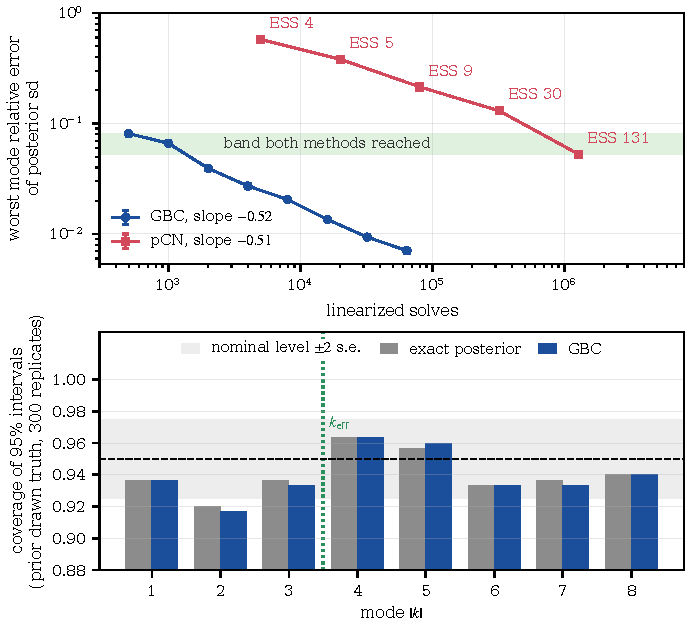
\includegraphics[width=0.94\textwidth]{mf_cost}
\caption{Upper panel: error against the number of linearized solves, on the metric the simulations actually control. GBC's posterior mean is exact at every budget in this model (Proposition~\ref{m:prop:linsuff}), so what is plotted is the error of the estimated posterior standard deviations, in units of the exact ones, taken as the largest over the retained modes and averaged over 40 replicates, for GBC at $M=250$ to $32000$ and for pCN at $5.0\times10^{3}$ to $1.3\times10^{6}$ iterations; the bars are one standard error over replicates, and the labels give the minimum over modes of the effective sample size (ESS) of the pCN chain, averaged over replicates. Both follow the Monte Carlo rate and neither has a floor. The shaded band is the range of accuracy both reached. Lower panel: coverage of nominal $95\%$ credible intervals by mode, over 300 replicates of the arm in which $\theta_0$ is drawn from the prior, for the exact posterior and for GBC; the shaded band is the nominal level plus or minus two binomial standard errors, and the dotted line marks $k_{\rm eff}$, beyond which the intervals are the prior's. Over the 2400 (replicate, mode) pairs of that arm the two disagree on 5 pairs against 3, each in a different replicate, a coverage difference of 0.0008 (Table~\ref{m:tab:cover}).}\label{m:fig:cost}
\end{figure}

\subsection{Coverage over replicates, in full}\label{m:sec:covstudy}

Table~\ref{m:tab:cover} has the numbers in full. Hypothesis (G1) of Assumption~\ref{m:ass:G} is stated in $P^\N_{\theta_0}$ probability at a \emph{fixed} $\theta_0$, and redrawing $\theta_0$ from the prior at every replicate makes the exact posterior's coverage nominal by construction, so under that design alone the comparison cannot fail informatively. The three arms are therefore $\theta_0$ redrawn from the prior, a fixed typical draw, and a fixed rough truth $\theta_{0,k}=(1+k^2)^{-1}\mathrm{sign}(\sin k)$, which the prior charges only in its tail. With $M=4000$ simulations, each arm has 300 replicates.

\begin{table}[t]\centering\footnotesize\setlength{\tabcolsep}{4pt}
\caption{Coverage of nominal $95\%$ credible intervals over 300 replicates per arm, by truth arm. ``All'' is over the $D=8$ retained modes, ``informed'' over the $k_{\rm eff}=3$ modes in which data precision exceeds prior precision. $b/c$ are the discordant counts, the (replicate, mode) pairs that the exact posterior covers and GBC misses and the reverse, out of $2400$. With $x_r$ the number of modes of replicate $r$ that the exact posterior covers and GBC misses minus the number of the reverse, $z=\sum_rx_r/(\sum_rx_r^2)^{1/2}$ is the clustered McNemar statistic of Durkalski and coauthors~\cite{durkalski2003}, and $p$ is the exact two sided $p$ value of the sign flip test, which gives each nonzero $x_r$ an independent random sign, as it has when the two methods are exchangeable within a replicate. The rough arm is misspecified by construction: its truth decays like $k^{-2}$, whereas a draw from the prior of smoothness $\alpha=3$ used here decays like $k^{-3}$, so both methods undercover, and identically; a draw from a prior with $\alpha>12$, the smoothness that Konen and Nickl~\cite{konennickl2026} require for the Navier Stokes problem, decays faster still. That the exact posterior undercovers too is the point of including the arm.}\label{m:tab:cover}
\begin{tabular}{>{\raggedright\arraybackslash}p{1.5in}ccccccc}
\toprule
& \multicolumn{2}{c}{All modes} & \multicolumn{2}{c}{Informed modes} & & & \\
\cmidrule(lr){2-3}\cmidrule(lr){4-5}
Truth arm & exact & GBC & exact & GBC & $b/c$ & $z$ & $p$\\
\midrule
$\theta_0\sim\Pi$, redrawn each replicate & 0.940 & 0.940 & 0.931 & 0.929 & $5$/$3$ & $0.71$ & $0.73$\\
fixed typical draw & 0.843 & 0.845 & 0.914 & 0.919 & $2$/$6$ & $-1.63$ & $0.22$\\
fixed rough truth & 0.251 & 0.251 & 0.670 & 0.670 & $1$/$1$ & $0.00$ & $1.00$\\
\bottomrule
\end{tabular}
\end{table}

Two things separate here. First, the exact posterior does not have frequentist coverage at a fixed truth and is not required to: its coverage over all $D$ retained modes falls from 0.940 on the prior drawn arm to 0.843 at the fixed typical draw and 0.251 at the rough one. That is the shrinkage of the posterior mean, milder on the informed modes, which averaging over the prior hides; as $N\to\infty$ each mode is covered at the nominal rate, with $D=8$ as here and, by Proposition~\ref{m:prop:regfixed}, with $D$ growing, but slowly at the rough truth.

Second, and this is the claim we make, GBC reproduces whatever the exact posterior does. Both methods are scored on the same replicate and the same mode, so the yardstick is a paired comparison, McNemar's, and not the binomial standard error of a single coverage estimate. The pairs of one replicate are not independent, since its eight modes are computed from the same data, so the comparison is made over the 300 independent replicates: the statistic of Table~\ref{m:tab:cover} is $z=\sum_rx_r/(\sum_rx_r^2)^{1/2}$. Where no replicate holds more than one discordant pair, as on the prior drawn and the rough arm, that statistic and its exact test are McNemar's own; on the typical arm one replicate holds one discordant pair of each kind. The standard error that the test gives the difference of the coverages, $(\sum_rx_r^2)^{1/2}/2400$, is between 11 and 21 times smaller than the binomial standard error at the nominal level of the coverage of a single mode over the 300 replicates, and between 5 and 7 times smaller than the standard error of the difference of the coverages over all modes of two methods run on independent data, so the test is several times more sensitive than the comparison it replaces. GBC survives it on every arm. The largest discrepancy across the three is 1.63 standard errors, on the typical arm, with exact $p$ value 0.22, and the largest difference in coverage over all modes is 0.0017; on the rough arm, where the exact posterior covers barely a quarter of the time, the two disagree on $2$ of $2400$ pairs, one each way.

The calibration claim is therefore relative rather than absolute: GBC reproduces the posterior it targets, including where that posterior is badly miscalibrated as a frequentist procedure. Coverage at a fixed truth is a property of the prior and the model rather than of the computation. One qualification: both arms of the comparison use the same summary, the adjoint statistic of Lemma~\ref{m:lem:adjoint}, and, by Proposition~\ref{m:prop:linsuff}, the same closed form posterior mean, so what differs between them is the covariance, exact in one case and estimated from the $M$ simulations in the other. The agreement is evidence that the estimated covariance is right, and is not a test of the summary or of the centering.

\subsection{A nonlinear check: two dimensional Navier Stokes}\label{m:sec:expns}

The experiments above are conjugate by design. This one is not, and it is the test that matters for Sections~\ref{m:sec:loc} and~\ref{m:sec:ns}: whether the localization theory survives contact with a nonlinear forward map. We solve \eqref{m:eq:nsproj} in vorticity form on the $2\pi$ periodic torus by a pseudospectral method with two thirds dealiasing and Heun stepping, on a $24^2$ grid with $\nu=5\times10^{-3}$, $T=1$ and $80$ steps; one forward solve costs about $15$\,ms. The unknown is the initial vorticity in $D=6$ real cosine modes with wavevectors $(1,0),(0,1),(1,1),(1,-1),(2,0),(0,2)$, the prior is independent Gaussian with standard deviations $1.5(\lambda_j/\lambda_1)^{-1}$, and the truth is a prior draw. The data are $N=80$ space time points with both velocity components observed, noise $\sigma=0.45$ against a signal of standard deviation about $0.95$, and observation times uniform on $[0,T]$, so the theory applies in its $T_0=0$ form. Accuracy is the per coordinate $\Wone_1$ distance to an adaptive random walk Metropolis reference, computed as the mean absolute difference of the two quantile functions at $199$ equally spaced levels from $0.005$ to $0.995$, normalized by that coordinate's posterior standard deviation and averaged over coordinates. The reference chain runs $6000$ iterations and keeps the last $4500$, with a Gaussian proposal of the Laplace covariance whose scale is adapted every $200$ iterations toward an acceptance rate of $0.30$; its effective sample size is about $250$ per coordinate. The generators of this section use the summary \eqref{m:eq:regsummary} at the maximum a posteriori estimate, with its Jacobian by finite differences (two Gauss Newton steps in the lower panel of Table~\ref{m:tab:ns}), and resample their training residuals rather than draw the Gaussian noise of Definition~\ref{m:def:gen}. The comparator is the Laplace approximation at the maximum a posteriori estimate, which in this six mode truncation is the finite sample form of the classical parametric Bernstein von Mises limit, the finite dimensional counterpart of the limit of Konen and Nickl~\cite{konennickl2026}, and is free: one Gauss Newton solve and one Hessian.

\begin{table}[tp]\centering\footnotesize
\caption{Two dimensional Navier Stokes, $D=6$, $N=80$. Distance to the Metropolis reference in units of posterior standard deviation, per coordinate and averaged; lower is better. The upper panel varies the architecture at $M=1600$, with a one step summary and, in the localized rows, radius $c=3$; the lower panel applies the three corrections of Section~\ref{m:sec:loc} in turn, at $c=5$, $M=1100$ and $k=2$ Gauss Newton steps (Remark~\ref{m:rem:nsdiag}). Every script scores against the same reference chain and draws its own Laplace sample, so the Laplace row moves between panels; across the six runs it lies between $0.076$ and $0.083$. The last row of that panel adds to the rescaled generator a shift of the center by the cubic correction of Remark~\ref{m:rem:relin}, the third derivative term of the Laplace expansion of the posterior mean, which is not a step of Algorithm~\ref{m:alg:loc}; on the same draws that shift raises the error of the rescaled generator from $0.070$ to $0.072$, that of the centered generator from $0.091$ to $0.092$ and that of the Laplace approximation from $0.078$ to $0.081$. Over twenty further resamplings of the $8000$ draws of the rescaled generator the shift raises its error in every one of them, by $0.002$ to $0.003$. The last line is not a method: it is the Monte Carlo standard error of the reference's own posterior mean.}\label{m:tab:ns}
\begin{tabular}{@{}>{\raggedright\arraybackslash}p{3.3in}c@{}}
\toprule
& \shortstack{$\Wone_1$ /\\ posterior s.d.}\\
\midrule
\multicolumn{2}{@{}l}{\emph{Architecture, $M=1600$}}\\
\quad training from the prior, identity head & 1.077\\
\quad training from the prior, learned affine head & 0.901\\
\quad training from the prior, $K=200$ nearest summaries, affine head & 0.364\\
\quad localized training, identity head & 0.187\\
\quad localized training, learned affine head & 0.180\\
\midrule
\multicolumn{2}{@{}l}{\emph{The corrections of Section~\ref{m:sec:loc}, $c=5$, $k=2$, $M=1100$}}\\
\quad localized, uncentered, spread as measured & 0.136\\
\quad $+$ residuals centered, Theorem~\ref{m:thm:locbias}(ii) & 0.092\\
\quad $+$ spread rescaled, Theorem~\ref{m:thm:locbias}(iii) & 0.070\\
\quad $+$ center shifted by the cubic correction, Remark~\ref{m:rem:relin} & 0.072\\
\midrule
Laplace at the maximum a posteriori estimate & 0.078\\
\midrule
\emph{Monte Carlo error of the reference itself} & \emph{0.063}\\
\bottomrule
\end{tabular}
\end{table}

Table~\ref{m:tab:ns} reads as a sequence of corrections, each one predicted by Section~\ref{m:sec:loc}.

\emph{Prior training with the identity head fails, and does not improve with $M$.} The error is about one posterior standard deviation and moves from 1.131 at $M=400$ to 1.078 at $M=800$ and 1.077 at $M=1600$, so it is bias and not Monte Carlo error. This is the shrinking neighborhood caveat of Remark~\ref{m:rem:affine} made concrete: the identity head is justified on the localization set, draws from the prior lie far outside it, and there the summary \eqref{m:eq:regsummary}, whose Jacobian sits at the preliminary estimate, is not a one step efficient estimator but an arbitrary linear functional. Learning an affine head instead recovers only part of the loss, because the map is genuinely nonlinear over the prior's support.

\emph{Localization is necessary, and post hoc localization is not a substitute.} Drawing the training parameters from a proposal centered at the preliminary estimate cuts the error by a factor of 5.8 and restores the decrease in $M$. Localizing a prior trained pool after the fact by keeping the $K$ nearest summaries reaches only 0.364 at $K=200$ and degrades as $K$ grows, which is the bias variance trade off of approximate Bayesian computation and is why Algorithm~\ref{m:alg:loc} localizes the proposal rather than the pool.

Two further knobs, importance weighting the localized draws back to the prior and relinearizing the summary, are reported in Remark~\ref{m:rem:nsdiag}.

\emph{The residual mean is the one Theorem~\ref{m:thm:locbias}(ii) predicts.} The uncentered head, which resamples the training residuals, adds their sample mean to the observed summary, and so displaces its center. Per coordinate that mean is right in sign and within $0.09$ posterior standard deviations in magnitude of the linear Gaussian prediction $P\bar\theta_N$ of Theorem~\ref{m:thm:locbias}(ii), the measured mean being the smaller in five of the six coordinates (both vectors are in Section~\ref{m:sec:loc}). We attribute the difference to the nonlinearity of the map; this run does not isolate it, since the sampling error of a mean of $M=1100$ residuals is about $0.03$ posterior standard deviations and four of the six differences are no larger than that. Centering removes it, at which point the center of the GBC posterior is displaced from the reference's own posterior mean by 0.061, which is exactly the maximum a posteriori estimate's displacement. Rescaling the spread by the reciprocal of the predicted inflation $(s_j+c^2p_j^2)^{1/2}$ of Theorem~\ref{m:thm:locbias}(iii) brings the error to 0.070, which is where Algorithm~\ref{m:alg:loc} stops; shifting the center as well, by the cubic correction described in the caption of Table~\ref{m:tab:ns}, gives 0.072, so that correction does not help here. In the last coordinate at $c=5$ the theorem predicts an inflation of 1.25, and the standard deviation of the residuals is measured at 1.25 times the Laplace standard deviation, which is 1.18 times the reference's.

Two further regimes were run, each with its own reference chain of $3000$ retained draws, to look for the crossover at which non Gaussianity of the posterior would favor a simulation based method. Both used $N=25$ space time points on $100$ time steps, $M=1200$ draws from a proposal of radius $c=2$, a one step summary and the identity head. The first raises the amplitude, the constant $1.5$ in the prior standard deviations raised to $2$, which raises the proxy $\max_j|\theta_{0,j}|/\nu$ of the advection to dissipation ratio of the realized truth from $185$ at the baseline constants to $246$, still below the $347$ of the main run's truth; the second widens the posterior, with noise standard deviation $1.30$ in place of $0.45$ and that constant raised to $3$ (proxy $370$). With the residuals neither centered nor rescaled, as in the runs recorded with our paper, GBC scored 0.105 and 0.253 against the Laplace approximation's 0.074 and 0.111. With the corrections of Section~\ref{m:sec:loc} applied to the same residuals, centering and then rescaling the spread, GBC scores 0.086 and then 0.080 in the first regime and 0.172 and then 0.114 in the second, so that the corrected generator ends 0.006 and 0.003 above the Laplace approximation, while the resampling noise of a single score is 0.003 to 0.004 for each method and the Monte Carlo standard errors of the two references are 0.081 and 0.083. The crossover was not found, and neither regime made the posterior measurably less Gaussian than the main run. Their mean absolute marginal skewness, 0.10 and 0.13, varies between chain seeds about as much as between regimes (from 0.06 to 0.10 in the first, from 0.07 to 0.13 in the second and from 0.09 to 0.12 at the baseline constants), and it is of the size that sampling error alone gives a Gaussian chain of that length and autocorrelation, 0.09 on average, with 0.05 to 0.15 between the 5th and 95th percentiles; the reference chain of the main run has 0.17, against 0.07 for a Gaussian chain like it. The uncorrected generator lost more in these regimes, where the prior fractions are larger, up to 0.36 and 0.65 against 0.17 in the main run: the displacement and inflation that the two corrections remove grow with the prior fraction (Theorem~\ref{m:thm:locbias}), and once they are removed, what separates GBC from the Laplace approximation is within the noise of the comparison. Both errors are governed by the curvature of $\Gcal$ measured in posterior standard deviations, so they do not move independently and the crossover cannot be assumed.

What the table does not show is a win. Corrected, GBC reaches 0.070 against the Laplace approximation's 0.078, but over resamplings of its own draws its error averages 0.077 with standard deviation 0.005, and the reference's own Monte Carlo standard error is 0.063, so the two are indistinguishable at the resolution available: bringing that standard error down to the size of the difference in the table would need a chain about sixty times longer. In this regime the Laplace approximation is excellent and free, and recommending a simulation based method on accuracy grounds would be wrong. What the table does show is that the distance between a naive GBC implementation and a correct one is a factor of 15 (1.077 at $M=1600$ against 0.070 at $M=1100$), and that every step of that factor is prescribed by Section~\ref{m:sec:loc} rather than being a tuning choice; the cubic correction of the last row is not one of those steps. The case for GBC here is amortization, and the regimes in which it is the only option are the ones the theory excludes: $T_0>0$, model error, non Gaussian noise.

\begin{remark}[Two diagnostics from the Navier Stokes run]\label{m:rem:nsdiag}
\emph{Importance weighting back to the prior degenerates, as the algorithm says it does.} Correcting the localized proposal by weights $w\propto\pi/q$ raises the error of the learned affine head, with the one step summary and $M=1200$, at every radius at which the algorithm operates: from 0.247 to 0.279 at $c=1$, from 0.175 to 0.387 at $c=2$, from 0.172 to 0.327 at $c=3$ and from 0.269 to 0.717 at $c=5$, with effective sample sizes of 29, 6.5, 15 and 1.5 out of $M$. At $c=8$ the weighted error, 0.377 at an effective sample size of 34, is below the unweighted 0.631; the statement concerns the radii $c\le5$ at which the algorithm operates. The proposal is much narrower than the prior, so the weights grow like $e^{+\norm\theta^2}$ in its tails. The unweighted estimator is biased for the prior based posterior, because the proposal acts as a prior on the training draws; in the linear Gaussian model the bias is of first order in the prior fraction (Theorem~\ref{m:thm:locbias}) and, for the affine head, in $c^{-2}$ as well, so it is small when the data dominate the prior and the radius is not small, while the weighted estimator's variance is not.

\emph{Linearizing the summary once is what the $c^4$ term of Proposition~\ref{m:prop:radius} costs.} At $c=2$ and $M=500$ the one step and two step Gauss Newton summaries are indistinguishable for the learned affine head, 0.169 against 0.171, as they must be where the $c^4$ term is negligible. At $c=6$ the one step summary costs that head a factor of 2.3, 0.370 against 0.162, and relinearizing recovers all of it (Remark~\ref{m:rem:relin} gives the iteration and its cost).
\end{remark}

\subsection{What these experiments do not establish}\label{m:sec:expnot}

Most of them are run on a linear, one dimensional, conjugate problem. Those test the summary, the generator and the resolution accounting of Sections~\ref{m:sec:suff}, \ref{m:sec:qnn} and \ref{m:sec:resolution}, and they cannot test the nonlinear theory at all. Section~\ref{m:sec:expns} supplies the nonlinear test. It is a six dimensional Galerkin truncation, which is a small problem; the comparison is against a Metropolis reference whose own Monte Carlo error is of the same size as the differences being reported; and the truth is a prior draw, so nothing there speaks to misspecification. What it does establish is that the three corrections of Section~\ref{m:sec:loc} are the ones that matter on a genuinely nonlinear map, in the direction and roughly the magnitude the theorems predict. Whether the same holds at operational resolution, where $D$ is in the thousands and the reference is unavailable, is left open. Section~\ref{m:sec:ns} remains a specification of the pipeline at the resolution the framework is stated for, not a report of a computation at that resolution.

\section{Nondissipative equations: Schr\"odinger}\label{m:sec:nondiss}

Every theorem so far uses dissipation twice: the parabolic semigroup makes the difference $\I_\theta-\Lcal$ two derivatives smoothing, which is what makes $\Kcal$ compact and allows Fredholm inversion of the information operator; and it makes $\I_{\theta_0}$ continuous from $H^{-k-2}$ into $\Ccal$, which is what lifts the weak topology theorem to the supremum norm.

\subsection{Linear Schr\"odinger}

Let $i\partial_tu=-\Delta u$ on $\T^d$, $u(0)=\theta\in L^2(\T^d;\C)$, so $u_\theta(t)=e^{it\Delta}\theta=\sum_je^{-i\lambda_jt}\theta_je_j$, and observe $Y_i=u_\theta(t_i,x_i)+\varepsilon_i$ with complex Gaussian noise. The forward map is unitary at every time, so the design matrix \eqref{m:eq:design} has $|s_j(t)|=1$ and
\begin{equation}\label{m:eq:schinfo}
\iota_j(T_0)=\frac1{T-T_0}\int_{T_0}^T|e^{-i\lambda_jt}|^2dt=1\qquad\text{for all }j\text{ and all }T_0 .
\end{equation}
\begin{itemize}[nosep]
\item There is no dissipation barrier. The observation window is irrelevant; Table~\ref{m:tab:iota} is replaced by a column of ones. The curvature constant $c_{\min}$ of the localized Langevin algorithm of Nickl and Wang~\cite{nicklwang2024} is $1$ uniformly in $D$ here, and since the forward map is linear and the information is $1$ in every mode, the expected Hessian of the negative log likelihood is $N\,\Id$ at every $\theta$ and gradient stability holds on all of the coefficient space, as for the heat equation in Section~\ref{sec:gradstab}. Their polynomial time guarantee is proved for a related steady state elliptic model, and verifying their remaining conditions for the initial condition of a time evolution equation is open as far as we know (Section~\ref{sec:gradstab}); if the guarantee carries over, the algorithm mixes in time polynomial in $D$ with no exponential factor, and dispersive is computationally easier than dissipative. For the linear equation itself no sampler is needed: the posterior is the Gaussian of Proposition~\ref{m:prop:sch}(a), and one Cholesky factorization of its $D\times D$ precision matrix gives exact draws.
\item The information operator is $T\cdot\Id$ in the unnormalized convention of \eqref{m:eq:modeinfo}; its inverse is bounded on $L^2$, and Condition 2E holds with $L^2$ in place of $H^{-1}$. The Bernstein von Mises limit for the initial condition is $\Ncal_{\theta_0}=N(0,T(\I^*\I)^{-1})=N(0,\Id)$, complex white noise on $\T^d$, tight on $H^{-a}$ for $a>d/2$ rather than $a>1+d/2$. The posterior on $\theta$ is Gaussian with a data independent covariance, so the posterior mean summary is sufficient, exactly and not only asymptotically, and the uniform statement of Assumption~\ref{m:ass:U}, which Theorem~\ref{m:thm:jwbvm} needs in general, is not required here; the sufficient statistic is again the adjoint evolution, with components $(\Phi^*Y)_j=\sum_ie^{i\lambda_jt_i}\overline{e_j(x_i)}Y_i$, i.e.\ the data run backward by the unitary group, and the GBC quantile map is affine, with the per mode scale of Proposition~\ref{m:prop:sch}(a). Statistically, the initial condition is recovered at the nonparametric rate of direct regression: no better than $\delta_N$ in $L^2$, since there is no sense in which the PDE constraint helps.
\item There is no supremum norm trajectory theorem. Since $u_\theta(t)=e^{it\Delta}\theta$ and $e^{it\Delta}$ is an isometry on every $H^s$, the state at time $t$ has exactly the regularity of the initial condition, the posterior standard deviation of $u_\theta(t,x)$ is $N^{-1/2}(\sum_j\sigma_j^2|e_j(x)|^2)^{1/2}$ with $\sigma_j^2=1$, and the series diverges at every $t$, not only at $t=0$. What survives is the weak topology theorem for the trajectory, $\Wone_{1,H^{-a}}$ at every $t$ (Proposition~\ref{m:prop:sch}(d)), and the regression analogue of the functional theorem that Castillo and Nickl~\cite{castillonickl2013} prove in Gaussian white noise: if $\Phi$ is twice differentiable on $L^2(\T^d;\C)$ with bounded second derivative and its derivative at $u_{\theta_0}(t)$ is $h\mapsto\mathrm{Re}\langle\psi,h\rangle$ with $\psi\in H^a$, $a>d/2$, then $\sqrt N(\Phi(u_{\tilde\theta_N}(t))-\Phi(u_{\theta_0}(t)))\to^dN(0,\norm\psi^2_{L^2})$, the efficient limit of Corollary~\ref{m:cor:schtransfer}(iv). Indeed the linear part is $\mathrm{Re}\langle e^{-it\Delta}\psi,\sqrt N(\tilde\theta_N-\theta_0)\rangle$, which has this limit by Proposition~\ref{m:prop:sch}(c), and the remainder is at most a constant times $\sqrt N\norm{\tilde\theta_N-\theta_0}^2_{L^2}$; the four terms in the proof of that proposition give $\norm{\tilde\theta_N-\theta_0}^2_{L^2}=O_P(D_N/N+\lambda_{D_N}^{-\gamma}+\delta_N^2)=O_P(\delta_N^2(\log N)^{2\gamma/d})$ for $D_N\asymp N^{d/(2\gamma+d)}/\log N$, and $\sqrt N\delta_N^2(\log N)^{2\gamma/d}\to0$ because $\gamma>d/2$.
\end{itemize}
The transfer theorem survives in a reduced form, Corollary~\ref{m:cor:schtransfer} below: Theorem~\ref{m:thm:main}(i) holds in $H^{-a}$, $a>d/2$, (ii) fails and is replaced by the weak topology statement at every $t$, and (iii) and (iv) hold for functionals that are differentiable on $H^{-a}$. Nickl's Conditions 1 and 2 are not invoked, and could not be: $\I^*\I=T\cdot\Id$ has order zero, so $\Delta\I^*\I$ is not a homeomorphism of any $H^\eta$ and Condition 2F fails.

\subsection{Cubic nonlinear Schr\"odinger}

Let $i\partial_tu+\Delta u=\kappa|u|^2u$ on $\T^d$, $d\le2$, $u(0)=\theta$; the cubic nonlinear Schr\"odinger equation (NLS) is globally well posed in $H^1$ for $\kappa>0$ (defocusing) and for small data when $\kappa<0$ (focusing). The linearization at $u_0=u_{\theta_0}$ is
\begin{equation}\label{m:eq:nlslin}
i\partial_tU+\Delta U=\kappa\big(2|u_0|^2U+u_0^2\bar U\big),\qquad U(0)=h .
\end{equation}
First, the potential term $2\kappa|u_0|^2U$ alone would generate a unitary flow: for any real potential $V(t,x)$, the solution operator of $i\partial_tU+\Delta U=VU$ is unitary on $L^2$, so its information operator over $[0,T]$ is exactly $T\cdot\Id$, and the potential contributes nothing to the Fisher information about the initial condition. Second, the conjugation term $\kappa u_0^2\bar U$ is real linear but not complex linear, and it is the sole source of departure from $T\cdot\Id$; it preserves the symplectic form $\mathrm{Im}\int U\bar W$ but not the $L^2$ norm.

\subsubsection{The plane wave background: Bogoliubov blocks} Take $\theta_0=a$ constant, so $u_0(t)=a\,e^{-i\kappa a^2t}$, and write $U=e^{-i\kappa a^2t}(\phi+i\psi)$ with $\phi,\psi$ real. Equation \eqref{m:eq:nlslin} becomes the real system $\partial_t\phi=-\Delta\psi$, $\partial_t\psi=\Delta\phi-2\kappa a^2\phi$, which decouples over Fourier modes $p$ into
\begin{equation}\label{m:eq:bog}
\begin{gathered}
\frac{d}{dt}\begin{pmatrix}\phi_p\\\psi_p\end{pmatrix}=A_p\begin{pmatrix}\phi_p\\\psi_p\end{pmatrix},\qquad A_p=\begin{pmatrix}0&|p|^2\\-(|p|^2+2\kappa a^2)&0\end{pmatrix},\\
\omega_p^2:=|p|^2\big(|p|^2+2\kappa a^2\big).
\end{gathered}
\end{equation}
Here $p=2\pi k$ with $k\in\Z^d$ is the wave vector of the mode $e^{2\pi ik\cdot x}$, so that $|p|^2=4\pi^2|k|^2$ is the eigenvalue of $-\Delta$ at that mode (the $\lambda_j$ of the earlier sections) and $|p|^2\ge\lambda_1=4\pi^2$ for $p\ne0$. The relation for $\omega_p^2$ is the Bogoliubov dispersion relation. For $\omega_p^2>0$ the propagator is $M_p(t)=\begin{pmatrix}\cos\omega_pt&r_p^{-1}\sin\omega_pt\\-r_p\sin\omega_pt&\cos\omega_pt\end{pmatrix}$ with $r_p=\omega_p/|p|^2=(1+2\kappa a^2/|p|^2)^{1/2}$; for $\omega_p^2<0$, which happens in the focusing case for $|p|^2<2|\kappa|a^2$, the block is hyperbolic: with $\gamma_p=|\omega_p|$ and $\rho_p=\gamma_p/|p|^2$ the propagator is
\[
M_p(t)=\begin{pmatrix}\cosh\gamma_pt&\rho_p^{-1}\sinh\gamma_pt\\\rho_p\sinh\gamma_pt&\cosh\gamma_pt\end{pmatrix},
\]
and this is the modulational (Benjamin Feir) instability.

\begin{proposition}[Information operator of NLS about a plane wave]\label{m:prop:bog}
With observations of $(\mathrm{Re}\,U,\mathrm{Im}\,U)$ uniformly on $[0,T]\times\T^d$, the information operator of the linearized model \eqref{m:eq:nlslin} at $\theta_0=a$ is block diagonal over Fourier modes with $2\times2$ blocks
\[
\Theta_p(T)=\int_0^TM_p(t)^\top M_p(t)\,dt .
\]
In the stable case $\omega_p^2>0$, with $r=r_p$ and $\omega=\omega_p$ (the degenerate block $p=0$ is in Lemma~\ref{m:lem:bogmin}(ii)),
\[
\begin{aligned}
\Theta_p(T)&=\frac T2\begin{pmatrix}1+r^2&0\\0&1+r^{-2}\end{pmatrix}+\frac{\sin2\omega T}{4\omega}\begin{pmatrix}1-r^2&0\\0&1-r^{-2}\end{pmatrix}\\
&\quad+\frac{\sin^2\omega T}{2\omega}\big(r^{-1}-r\big)\begin{pmatrix}0&1\\1&0\end{pmatrix},
\end{aligned}
\]
so that $\Theta_p(T)=T\cdot\Id+O\big(\kappa a^2T/|p|^2\big)+O(|p|^{-2})$ as $|p|\to\infty$, with $\det\Theta_p(T)\ge T^2$ for every $p$ and every $T>0$, by Lemma~\ref{m:lem:bogmin}(i). In the unstable case $\omega_p^2<0$, with $\gamma=\gamma_p$ and $\rho=\rho_p$, the same formula holds after the substitution $\omega\mapsto i\gamma$, $r\mapsto i\rho$, that is
\[
\begin{aligned}
\Theta_p(T)&=\frac T2\begin{pmatrix}1-\rho^2&0\\0&1-\rho^{-2}\end{pmatrix}+\frac{\sinh2\gamma T}{4\gamma}\begin{pmatrix}1+\rho^2&0\\0&1+\rho^{-2}\end{pmatrix}\\
&\quad+\frac{\sinh^2\gamma T}{2\gamma}\big(\rho+\rho^{-1}\big)\begin{pmatrix}0&1\\1&0\end{pmatrix},
\end{aligned}
\]
and as $\gamma T\to\infty$ its largest eigenvalue is asymptotic to $(\rho+\rho^{-1})^2e^{2\gamma T}/(8\gamma)$ while its smallest eigenvalue tends to $1/(2\gamma)$.
\end{proposition}

\begin{proof}
Block diagonality is \eqref{m:eq:bog} together with orthogonality of the Fourier modes under the uniform design, exactly as in \eqref{m:eq:gram}. The entries are the integrals $\int_0^T\cos^2$, $\int_0^T\sin^2$, $\int_0^T\sin\cos$ of $\omega_pt$ with the weights read off from $M_p^\top M_p$, namely $\cos^2+r^2\sin^2$, $\cos^2+r^{-2}\sin^2$ on the diagonal and $(r^{-1}-r)\sin\cos$ off it. The determinant bound is not an estimate on the leading term but an identity: the generator in \eqref{m:eq:bog} is traceless, so $\det M_p(t)=1$ for every $t$, and superadditivity of $\det^{1/2}$ on the positive semidefinite cone gives $\det\Theta_p(T)\ge T^2$ for all $p$ and all $T$, with the explicit deficit computed in Lemma~\ref{m:lem:bogmin}(ii). The hyperbolic case is the same computation with $\cosh\gamma_pt,\sinh\gamma_pt$ in place of $\cos\omega_pt,\sin\omega_pt$: the weights are $\cosh^2+\rho^2\sinh^2$, $\cosh^2+\rho^{-2}\sinh^2$ on the diagonal and $(\rho+\rho^{-1})\sinh\cosh$ off it, and the trace grows like $(\rho+\rho^{-1})^2e^{2\gamma T}/(8\gamma)$. The smaller eigenvalue is $\det\Theta_p(T)/\lambda_{\max}$, which tends to $1/(2\gamma)$ by Lemma~\ref{m:lem:bogmin}(vi).
\end{proof}

\begin{figure}[t]\centering
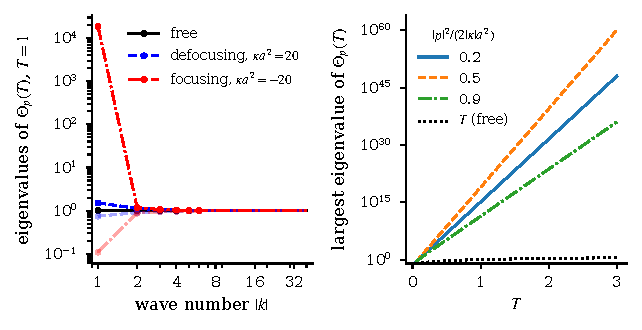
\includegraphics[width=\textwidth]{mf_nls}
\caption{Left: the two eigenvalues of the per pair information block $\Theta_p(T)$ of Proposition~\ref{m:prop:bog} at $T=1$ against the wave number $|k|$, where $|p|^2=4\pi^2|k|^2$; the larger eigenvalue is the dark curve and the smaller the pale curve of the same style. Free flow: both equal $T$. Defocusing case $\kappa a^2=20$: a compact perturbation decaying like $|p|^{-2}$, with eigenvalues $0.746$ and $1.511$ at $|k|=1$ and $0.998$ and $1.002$ at $|k|=16$. Focusing case $\kappa a^2=-20$: the mode $|k|=1$ lies inside the modulational band, $|p|^2=\lambda_1=4\pi^2<2|\kappa|a^2=40$, and its eigenvalues are $0.109$ and $1.87\times10^4$, so the larger one is amplified and the smaller one stays of order $1/(2\gamma_p)$. Right: growth in $T$ of the largest eigenvalue for $|p|^2/(2|\kappa|a^2)=0.2$, $0.5$, $0.9$ in the unstable band with $\kappa a^2=-0.6\lambda_1$ (on the unit torus only $|k|=1$ lies in this band, at the ratio $0.83$, so the three values illustrate the growth law rather than particular modes), against the free value $T$. Modulational instability amplifies the information about the initial condition exponentially along one direction, the opposite of the viscous curse of Table~\ref{m:tab:iota}.}\label{m:fig:nls}
\end{figure}

The consequences for the theory, illustrated in Figure~\ref{m:fig:nls}:
\begin{itemize}[nosep]
\item Defocusing. $\I^*_{\theta_0}\I_{\theta_0}=T\cdot\Id+\Kcal$ with $\Kcal$ block diagonal, $\norm{\Kcal_p}=O(\kappa a^2T/|p|^2)$, hence compact and two derivatives smoothing, which is the same order as in the parabolic case. Lemma~\ref{m:lem:bogmin} bounds the smallest eigenvalue of every block below, uniformly in $p$, so $\I^*_{\theta_0}\I_{\theta_0}$ is bounded above and below on $L^2$ and on every $H^\eta$, with explicit constants (Corollary~\ref{m:cor:condE}(a)). This is the analogue of Condition 2F without the factor $\Delta$, with $\eta_0=0$. The same bound is a stability estimate for the \emph{linearization} (Corollary~\ref{m:cor:condE}(b)). It is not Condition 2E, which is a lower bound on the increments of the nonlinear map $\Gcal$ and follows instead from an energy estimate for the difference of two solutions (Proposition~\ref{m:prop:nlsstab}); Remark~\ref{m:rem:condEgap} states precisely what is and is not verified. Granting the remaining conditions, the Bernstein von Mises limit is $\Ncal_{\theta_0}=N(0,T\diag\Theta_p(T)^{-1})$, whose per block covariance $T\Theta_p(T)^{-1}$ is bounded uniformly in $p$ \emph{and} in $T$ (Corollary~\ref{m:cor:condE}(c)); the limit is tight on $H^{-a}$ for $a>d/2$, and the trajectory theorem holds in weak topologies and for functionals but not in supremum norm, as in the linear case.
\item Focusing. For modes with $|p|^2<2|\kappa|a^2$ the largest eigenvalue of the block grows like $e^{2\gamma_pT}$ (Proposition~\ref{m:prop:bog}), so the component of the initial condition along the corresponding eigenvector is recovered with variance of order $Te^{-2\gamma_pT}/N$: the instability amplifies information, but along one direction of each unstable block only. The other direction is damped by the same flow, the smallest eigenvalue stays near $1/(2\gamma_p)$ (Lemma~\ref{m:lem:bogmin}(vi)), and the variance of that component is of order $2\gamma_pT/N$, which grows with $T$. There are finitely many such modes, so the tightness of the limit is not affected. The price is that the constants in Conditions 2A and 2D, which concern the nonlinear map, and the quadratic remainder of Condition 2C can be expected to grow with $T$, so that the localization set of Theorem~3 of Nickl~\cite{nicklbvm2024} would have to shrink accordingly; a Bernstein von Mises theorem can be expected only for $T$ fixed and $N\to\infty$, with constants exponential in $\gamma_{\max}T$. Computationally the curvature constant $c_{\min}$ of Nickl and Wang, the smallest eigenvalue of the normalized block $\Theta_p(T)/T$, does not become large: it is of order $1/(2\gamma_pT)$, and the amplification appears instead in the condition number $\lambda_{\max}/\lambda_{\min}$ of the block (Lemma~\ref{m:lem:bogmin}(vi)).
\item General backgrounds. For $u_0$ with several Fourier modes the conjugation term couples $p$ to $2k_0-p$ for every mode $k_0$ of $u_0$, and the time integrals in $\I^*\I$ are of the form $\int_0^Te^{i(\lambda_{p}+\lambda_{p'}-\lambda_{k_0}-\lambda_{k_0'})t}dt$: they are $O(1)$ on the four wave resonant manifold $\lambda_{k_1}+\lambda_{k_2}=\lambda_{k_3}+\lambda_{k_4}$, $k_1+k_2=k_3+k_4$, and $O(1/|\text{mismatch}|)$ off it. The resonant part is not compact in general; on $\T^2$ the resonant manifold is large. This is the structure that the wave turbulence derivation of Deng and Hani~\cite{denghani2023} exploits, and the invertibility of the information operator for a general NLS background is a question about the same resonant sums.
\item Sufficient statistic and GBC. Unchanged in form: the one step statistic \eqref{m:eq:onestep} with the adjoint of \eqref{m:eq:nlslin}, with $u_0=u_{\bar\theta_N}$. For the real inner product $\mathrm{Re}\int A\bar B$, multiplication by $i$ is skew and $U\mapsto c\bar U$ is self adjoint for every function $c$, so the adjoint of the generator $U\mapsto i\Delta U-i\kappa(2|u_0|^2U+u_0^2\bar U)$ of \eqref{m:eq:nlslin} is $W\mapsto-i\Delta W+i\kappa(2|u_0|^2W-u_0^2\bar W)$. Hence, for a source $g$ on $\mathcal X$, in \eqref{m:eq:onestep} the residuals $\sum_{i\in\mathcal I}r_i\,\delta_{X_i}$, the adjoint is $\I^*g=W(0)$, where $W$ solves the backward problem $i\partial_tW+\Delta W=\kappa(2|u_0|^2W-u_0^2\bar W)-ig$, $W(T)=0$: then $\frac{d}{dt}\mathrm{Re}\langle U,W\rangle=-\mathrm{Re}\langle U,g\rangle$ for the solution $U$ of \eqref{m:eq:nlslin}, so that $\int_0^T\mathrm{Re}\langle U(t),g(t)\rangle dt=\mathrm{Re}\langle h,W(0)\rangle$. If a Bernstein von Mises theorem holds (Remark~\ref{m:rem:condEgap}), the GBC quantile map is asymptotically affine with per pair scale $T\Theta_p(T)^{-1}/N$ about a plane wave, and a generator with $2\times2$ block structure over Fourier pairs is exact to leading order.
\end{itemize}

\subsubsection{The smallest eigenvalue of a Bogoliubov block} The blocks of Proposition~\ref{m:prop:bog} are $2\times2$, so their spectrum is determined by two scalars, and the determinant is fixed by a conservation law rather than by a computation: the Bogoliubov flow is area preserving, $\det M_p(t)=1$ for every $p$ and every $t$, in the elliptic, hyperbolic and degenerate cases alike. This is the linearized form of the conservation of the symplectic form $\mathrm{Im}\int U\bar W$ noted after \eqref{m:eq:nlslin}.

\begin{lemma}[Determinant, trace and smallest eigenvalue of $\Theta_p(T)$]\label{m:lem:bogmin}
Let $\Theta_p(T)=\int_0^TM_p(t)^\top M_p(t)\,dt$ be the block of Proposition~\ref{m:prop:bog}, and write $\omega=\omega_p$, $r=r_p=\omega_p/|p|^2$ in the elliptic case $\omega_p^2>0$, and $\gamma=\gamma_p=|\omega_p|$, $\rho=\rho_p=\gamma_p/|p|^2$ in the hyperbolic case $\omega_p^2<0$. Then, for every $T>0$:
\begin{enumerate}[label=(\roman*),nosep,leftmargin=2.2em]
\item $\det M_p(t)=1$ for all $t$, and consequently
\[
\det\Theta_p(T)\ \ge\ T^2\qquad\text{for every }p\text{ and every }T>0,
\]
with no restriction on $\omega_pT$.
\item Explicitly, for $p\ne0$ in the elliptic case,
\[
\det\Theta_p(T)=T^2+\frac{(r-r^{-1})^2}{4}\Big(T^2-\frac{\sin^2\omega T}{\omega^2}\Big),
\]
and in the hyperbolic case $\det\Theta_p(T)=T^2+\frac{(\rho+\rho^{-1})^2}{4}\big(\gamma^{-2}\sinh^2\gamma T-T^2\big)$, which is the analytic continuation $\omega\mapsto i\gamma$, $r\mapsto i\rho$ of the first formula. At $p=0$, $\Theta_0(T)=T\left(\begin{smallmatrix}1+\frac43s^2&-s\\-s&1\end{smallmatrix}\right)$ with $s=\kappa a^2T$, so $\det\Theta_0(T)=T^2(1+\tfrac13s^2)$.
\item In the elliptic case $\tr\,\Theta_p(T)=2T+(r-r^{-1})^2\int_0^T\sin^2\omega t\,dt\le T(r^2+r^{-2})$, and $\tr\,\Theta_0(T)=T(2+\tfrac43s^2)$.
\item Since $\Theta_p(T)$ is a positive definite $2\times2$ matrix, $\lambda_{\min}=\det/\lambda_{\max}\ge\det/\tr$, whence in the elliptic case
\[
\lambda_{\min}\big(\Theta_p(T)\big)\ \ge\ \frac{T}{r_p^2+r_p^{-2}},\qquad\text{and}\qquad \lambda_{\min}\big(\Theta_0(T)\big)\ \ge\ \frac T4 .
\]
If $r_p\ge1$ this implies $\lambda_{\min}\ge T/(1+r_p^2)$; if $r_p<1$ the form $T/(1+r_p^2)$ is false, so $r_p^2+r_p^{-2}$ cannot be replaced by $1+r_p^2$ in general.
\item Defocusing case, $\kappa>0$. Then $1<r_p^2\le1+2\kappa a^2/\lambda_1$ for $p\ne0$, with $\lambda_1=4\pi^2$ the smallest nonzero eigenvalue of $-\Delta$, and
\[
\begin{gathered}
\inf_p\lambda_{\min}\big(\Theta_p(T)\big)\ \ge\ \frac{T\lambda_1}{4(\lambda_1+\kappa a^2)},\\
\sup_{p\ne0}\lambda_{\max}\big(\Theta_p(T)\big)\ \le\ \frac{2T(\lambda_1+\kappa a^2)}{\lambda_1}.
\end{gathered}
\]
\item Focusing band, $\omega_p^2<0$. As $\gamma_pT\to\infty$, $\lambda_{\max}\big(\Theta_p(T)\big)\sim\tr\,\Theta_p(T)\sim(\rho_p+\rho_p^{-1})^2e^{2\gamma_pT}/(8\gamma_p)$ and $\lambda_{\min}\big(\Theta_p(T)\big)=\det\Theta_p(T)/\lambda_{\max}\to1/(2\gamma_p)$. The bound $\lambda_{\min}\ge T^2/\tr\,\Theta_p(T)$ still holds but is exponentially small in $\gamma_pT$, so it is far from sharp: the amplification is confined to one eigendirection, and the block is well conditioned in determinant and badly conditioned in ratio, with condition number $\lambda_{\max}/\lambda_{\min}\sim\frac14(\rho_p+\rho_p^{-1})^2e^{2\gamma_pT}$.
\end{enumerate}
\end{lemma}

\begin{proof}
(i) The generator $A_p$ in \eqref{m:eq:bog} has $\tr\,A_p=0$, so Liouville's formula gives $\det M_p(t)=e^{t\,\tr\,A_p}=1$. Hence $P(t):=M_p(t)^\top M_p(t)$ is symmetric positive definite with $\det P(t)=1$ for every $t$. Minkowski's determinant inequality, $\det(A+B)^{1/2}\ge(\det A)^{1/2}+(\det B)^{1/2}$ for positive semidefinite $2\times2$ matrices $A,B$, says that $P\mapsto(\det P)^{1/2}$ is superadditive on the cone; applying it to Riemann sums for $\int_0^TP(t)\,dt$ and passing to the limit,
\[
\big(\det\Theta_p(T)\big)^{1/2}\ \ge\ \int_0^T\big(\det P(t)\big)^{1/2}dt\ =\ T .
\]

(ii) to (iii) Write $C=\cos\omega t$, $S=\sin\omega t$ and
\[
\begin{gathered}
\alpha=\int_0^TC^2=\frac T2+\frac{\sin2\omega T}{4\omega},\qquad
\beta=\int_0^TS^2=\frac T2-\frac{\sin2\omega T}{4\omega},\\
\mu=\int_0^TSC=\frac{\sin^2\omega T}{2\omega},
\end{gathered}
\]
so that $\alpha+\beta=T$. By the entries of $M_p^\top M_p$ recorded in Proposition~\ref{m:prop:bog}, $\Theta_{11}=\alpha+r^2\beta$, $\Theta_{22}=\alpha+r^{-2}\beta$ and $\Theta_{12}=(r^{-1}-r)\mu$. Using $r^2+r^{-2}=2+(r-r^{-1})^2$,
\[
\begin{aligned}
\det\Theta_p&=(\alpha+r^2\beta)(\alpha+r^{-2}\beta)-(r-r^{-1})^2\mu^2\\
&=(\alpha+\beta)^2+(r-r^{-1})^2\big(\alpha\beta-\mu^2\big),
\end{aligned}
\]
and, with $\sin^22\omega T=4\sin^2\omega T\cos^2\omega T$,
\[
\begin{aligned}
\alpha\beta-\mu^2&=\frac{T^2}4-\frac{\sin^22\omega T}{16\omega^2}-\frac{\sin^4\omega T}{4\omega^2}\\
&=\frac{T^2}4-\frac{\sin^2\omega T}{4\omega^2}\big(\cos^2\omega T+\sin^2\omega T\big)
=\frac14\Big(T^2-\frac{\sin^2\omega T}{\omega^2}\Big),
\end{aligned}
\]
which is the stated determinant and, since $|\sin x|\le|x|$, recovers $\det\Theta_p\ge T^2$ with the deficit exhibited. Likewise $\tr\,\Theta_p=2\alpha+(r^2+r^{-2})\beta=2(\alpha+\beta)+(r-r^{-1})^2\beta=2T+(r-r^{-1})^2\beta$, and $\beta\le T$ gives $\tr\,\Theta_p\le T\big(2+(r-r^{-1})^2\big)=T(r^2+r^{-2})$. The hyperbolic case is the same computation with $C,S$ replaced by $\cosh\gamma t,\sinh\gamma t$. The diagonal weights of $M_p^\top M_p$ are then $\cosh^2+\rho^2\sinh^2$ and $\cosh^2+\rho^{-2}\sinh^2$, the off diagonal weight is $(\rho+\rho^{-1})\sinh\cosh$ in place of $(r^{-1}-r)\sin\cos$, and with
\[
\begin{gathered}
\alpha_h=\int_0^T\cosh^2\gamma t\,dt=\frac T2+\frac{\sinh2\gamma T}{4\gamma},\\
\beta_h=\int_0^T\sinh^2\gamma t\,dt=-\frac T2+\frac{\sinh2\gamma T}{4\gamma},\\
\mu_h=\int_0^T\sinh\gamma t\cosh\gamma t\,dt=\frac{\sinh^2\gamma T}{2\gamma}
\end{gathered}
\]
one has $\alpha_h-\beta_h=T$ in place of $\alpha+\beta=T$, $\det\Theta_p=(\alpha_h-\beta_h)^2+(\rho+\rho^{-1})^2(\alpha_h\beta_h-\mu_h^2)$, $\tr\,\Theta_p=2\alpha_h+(\rho^2+\rho^{-2})\beta_h$, and $\alpha_h\beta_h-\mu_h^2=\frac14(\gamma^{-2}\sinh^2\gamma T-T^2)\ge0$ because $\sinh x\ge x$. At $p=0$ the generator is nilpotent, $M_0(t)=\left(\begin{smallmatrix}1&0\\-2\kappa a^2t&1\end{smallmatrix}\right)$, and integrating $M_0^\top M_0$ gives the stated $\Theta_0(T)$.

(iv) For a positive definite $2\times2$ matrix, $\lambda_{\min}\lambda_{\max}=\det$ and $\lambda_{\max}\le\lambda_{\min}+\lambda_{\max}=\tr$, so $\lambda_{\min}=\det/\lambda_{\max}\ge\det/\tr$; combining (i) and (iii) gives $\lambda_{\min}\ge T^2/\big(T(r^2+r^{-2})\big)$. At $p=0$, $\det/\tr=T(3+s^2)/(6+4s^2)$, which decreases from $T/2$ at $s=0$ to $T/4$ as $s\to\infty$ and is therefore always at least $T/4$. For $r\ge1$ one has $r^{-2}\le1$, so $r^2+r^{-2}\le1+r^2$ and the weaker bound follows; for $r<1$ the inequality reverses and $T/(1+r^2)$ is not a valid bound: as $r\downarrow0$ with $|p|^2$ fixed, $M_p(t)\to\left(\begin{smallmatrix}1&|p|^2t\\0&1\end{smallmatrix}\right)$, for which $\det\Theta_p=T^2+|p|^4T^4/12$ and $\tr\,\Theta_p=2T+|p|^4T^3/3$, so $\lambda_{\min}\to T/4$ as $|p|^2T\to\infty$ while $T/(1+r^2)\to T$.

(v) In the defocusing case $r_p^2=1+2\kappa a^2/|p|^2>1$ is decreasing in $|p|$, hence $r_p^2\le R:=1+2\kappa a^2/\lambda_1$ for $p\ne0$; $x\mapsto x+x^{-1}$ is increasing on $[1,\infty)$, so $r_p^2+r_p^{-2}\le R+R^{-1}\le R+1=2(\lambda_1+\kappa a^2)/\lambda_1$, and (iv) gives $\lambda_{\min}\ge T\lambda_1/\big(2(\lambda_1+\kappa a^2)\big)$ for $p\ne0$. That exceeds $T\lambda_1/\big(4(\lambda_1+\kappa a^2)\big)$, and so does the bound $T/4$ at $p=0$ because $\lambda_1<\lambda_1+\kappa a^2$; taking the minimum over the two cases gives the first display. The second is $\lambda_{\max}\le\tr\,\Theta_p\le T(r_p^2+r_p^{-2})$ with the same estimate.

(vi) By (ii) and $\sinh^2x\sim e^{2x}/4$, $\det\Theta_p(T)\sim(\rho+\rho^{-1})^2e^{2\gamma T}/(16\gamma^2)$, and since $\alpha_h,\beta_h\sim e^{2\gamma T}/(8\gamma)$, $\tr\,\Theta_p(T)=2\alpha_h+(\rho^2+\rho^{-2})\beta_h\sim(2+\rho^2+\rho^{-2})e^{2\gamma T}/(8\gamma)=(\rho+\rho^{-1})^2e^{2\gamma T}/(8\gamma)$. Hence $\det/\tr\to1/(2\gamma)$ and $\det/\tr^2\to0$, and from $\lambda_{\min}=2\det/\big(\tr+\sqrt{\tr^2-4\det}\big)$ we get $\lambda_{\min}=(\det/\tr)(1+o(1))\to1/(2\gamma)$ and $\lambda_{\max}=\tr\,(1+o(1))$. The condition number is $\lambda_{\max}/\lambda_{\min}=\lambda_{\max}^2/\det\sim\frac14(\rho+\rho^{-1})^2e^{2\gamma T}$.
\end{proof}

If observation starts at $T_0>0$, the information on $[T_0,T]$ is $\int_{T_0}^TM_p^\top M_p\,dt$, and Lemma~\ref{m:lem:bogmin} says what survives. For a stable mode with $p\ne0$ the proofs of (i), (iii) and (iv) use only $\det M_p(t)=1$ and the pointwise bound $\tr\big(M_p(t)^\top M_p(t)\big)\le r_p^2+r_p^{-2}$, so the bounds hold with $T$ replaced by $T-T_0$: the position of the window does not enter them, as in the linear case. Two things change. In the focusing band the damped eigenvector $v$ of $A_p$ satisfies $M_p(t)v=e^{-\gamma_pt}v$, so the Rayleigh quotient gives $\lambda_{\min}\big(\int_{T_0}^TM_p^\top M_p\,dt\big)\le e^{-2\gamma_pT_0}/(2\gamma_p)$: a late window loses the information along the damped direction, as in the dissipation barrier of Table~\ref{m:tab:iota}, but for the finitely many unstable modes only (for $\kappa a^2=-20$, $|k|=1$ and windows of length one the bound is sharp to within one percent). At $p=0$ the shear $M_0(t)$ grows linearly: with $\tau=T-T_0$ the window block has determinant $\tau^2\big(1+\tfrac13\kappa^2a^4\tau^2\big)$ and trace $\tau\big(2+\tfrac43\kappa^2a^4(T^2+TT_0+T_0^2)\big)$, so its smallest eigenvalue decays like $T_0^{-2}$, for the single mode $p=0$.

\begin{corollary}[Linearized stability and the analogue of Condition 2F for the defocusing plane wave]\label{m:cor:condE}
Let $\kappa>0$, $\theta_0=a$ constant, and let $\I_{\theta_0}$ be the linearization \eqref{m:eq:nlslin}, with adjoint taken with respect to unnormalized $L^2(\mathcal X)$, $\mathcal X=[0,T]\times\T^d$. Set
\[
c_\star^2=\frac{T\lambda_1}{4(\lambda_1+\kappa a^2)},\qquad
C_\star^2=\max\Big\{\frac{2T(\lambda_1+\kappa a^2)}{\lambda_1},\ T\big(2+\tfrac43\kappa^2a^4T^2\big)\Big\}.
\]
Then for every $h\in L^2(\T^d;\C)$,
\[
c_\star^2\norm{h}_{L^2(\Omega)}^2\ \le\ \norm{\I_{\theta_0}h}^2_{L^2(\mathcal X)}=\big\langle h,\I^*_{\theta_0}\I_{\theta_0}h\big\rangle\ \le\ C_\star^2\norm{h}_{L^2(\Omega)}^2,
\]
and consequently
\begin{enumerate}[label=(\alph*),nosep,leftmargin=2.2em]
\item $\I^*_{\theta_0}\I_{\theta_0}$ is a homeomorphism of $H^\eta(\T^d)$ for every $\eta\in\R$, with the explicit constants $c_\star^2,C_\star^2$; this is the analogue of Condition 2F without the factor $\Delta$, with $\eta_0=0$, and no smoothing is needed, while Condition 2F as stated fails, since $\Delta\I^*_{\theta_0}\I_{\theta_0}$ loses two derivatives;
\item the linearization satisfies the stability estimate
\[
\norm{\I_{\theta_0}h}_{L^2(\mathcal X)}\ \ge\ c_\star\norm{h}_{L^2(\Omega)}\ \ge\ c_\star\norm{h}_{H^{-1}(\Omega)} ,
\]
which is the estimate of Condition 2E with $\I_{\theta_0}$ in place of $\Gcal$, in the stronger norm $L^2$ rather than $H^{-1}$;
\item $\Ncal_{\theta_0}=N\big(0,T(\I^*_{\theta_0}\I_{\theta_0})^{-1}\big)=N\big(0,T\diag\Theta_p(T)^{-1}\big)$ has per block covariance $T\Theta_p(T)^{-1}$ with
\[
\norm{T\Theta_p(T)^{-1}}\ \le\ \frac{T}{\lambda_{\min}(\Theta_p(T))}\ \le\ \frac{4(\lambda_1+\kappa a^2)}{\lambda_1}
\]
uniformly in $p$ and in $T$, so $\Ncal_{\theta_0}$ is tight on $H^{-a}$ for $a>d/2$; contrast the parabolic case, where $1/\iota_j\asymp2\nu\lambda_jT$ diverges with $j$ and with $T$.
\end{enumerate}
\end{corollary}

\begin{proof}
The Bogoliubov substitution $U=e^{-i\kappa a^2t}(\phi+i\psi)$ is at each $t$ a pointwise rotation of $\C\cong\R^2$, hence an isometry of $L^2(\T^d;\C)$, and $\norm{h}^2_{L^2(\Omega)}=\norm{\phi(0)}^2+\norm{\psi(0)}^2$ for $h=U(0)$, the norms being those of the real functions $\phi(0),\psi(0)$. Because the design is uniform on $\mathcal X$, whose measure is $T$, and the adjoint is unnormalized,
\[
\begin{aligned}
\norm{\I_{\theta_0}h}^2_{L^2(\mathcal X)}&=\int_0^T\norm{U(t)}^2_{L^2(\T^d)}dt=\sum_p\int_0^T\big|M_p(t)v_p\big|^2dt\\
&=\sum_p\big\langle v_p,\Theta_p(T)v_p\big\rangle,\qquad v_p=\big(\phi_p(0),\psi_p(0)\big),
\end{aligned}
\]
with $\sum_p|v_p|^2=\norm{h}^2_{L^2(\Omega)}$ by Parseval. The two sided bound is Lemma~\ref{m:lem:bogmin}(v) applied term by term, together with $\lambda_{\max}(\Theta_0(T))\le\tr\,\Theta_0(T)=T(2+\frac43\kappa^2a^4T^2)$ for the zero mode. For (a), each block acts within a single $p$ and therefore commutes with the Sobolev weights $(1+\lambda_p)^{\eta/2}$, so the two sided bound on $L^2$ transfers to $H^\eta$ for every $\eta$. Part (b) is the left inequality together with $\norm{h}_{H^{-1}}\le\norm{h}_{L^2}$. Part (c) is the block inverse, with tightness as in Proposition~\ref{m:prop:sch}: $\sum_p\lambda_p^{-a}<\infty$ for $a>d/2$.
\end{proof}

The stability estimate for $\Gcal$ itself does not go through the linearization.

\begin{proposition}[Stability of the cubic NLS solution map]\label{m:prop:nlsstab}
Let $\kappa\ne0$, let $u$ and $v$ solve $i\partial_tu+\Delta u=\kappa|u|^2u$ on $[0,T]\times\T^d$ with data $\theta$ and $\vartheta$, in $H^1$ if $d=1$ and in $H^2$ if $d=2$, and suppose that $\norm{u(t)}_{L^\infty}\le M_\infty$ and $\norm{v(t)}_{L^\infty}\le M_\infty$ for $t\le T$, with $M_\infty>0$. Then, for $t\le T$,
\[
e^{-6|\kappa|M_\infty^2t}\norm{\theta-\vartheta}^2_{L^2(\Omega)}\ \le\ \norm{u(t)-v(t)}^2_{L^2(\Omega)}\ \le\ e^{6|\kappa|M_\infty^2t}\norm{\theta-\vartheta}^2_{L^2(\Omega)},
\]
and, with the unnormalized $L^2(\mathcal X)$ of Corollary~\ref{m:cor:condE},
\[
\begin{aligned}
\norm{\Gcal(\theta)-\Gcal(\vartheta)}^2_{L^2(\mathcal X)}&\ge\frac{1-e^{-6|\kappa|M_\infty^2T}}{6|\kappa|M_\infty^2}\norm{\theta-\vartheta}^2_{L^2(\Omega)}\\
&\ge Te^{-6|\kappa|M_\infty^2T}\norm{\theta-\vartheta}^2_{H^{-1}(\Omega)} .
\end{aligned}
\]
A bound $M_\infty=M_\infty(T,\kappa,B)$ that holds for all data in a ball of radius $B$ exists in each of the following cases:
\begin{enumerate}[label=(\alph*),nosep,leftmargin=2.2em]
\item $d=1$, either sign of $\kappa$, every ball of $H^1$;
\item $d=2$, $\kappa>0$, every ball of $H^2$;
\item $d=2$, $\kappa<0$, the balls of $H^2$ with $2|\kappa|C_2B^2T<1$, where $C_2$ is a constant such that $\norm{|f|^2f}_{H^2}\le C_2\norm f^3_{H^2}$.
\end{enumerate}
On such a ball, Condition 2E therefore holds for $\Gcal$, with the stronger norm $L^2$ on the right and the constant $T^{1/2}e^{-3|\kappa|M_\infty^2T}$, Condition 2A holds with the bound $M_\infty$, and the upper bound gives the $L^2$ Lipschitz estimate of Condition 2B, $\norm{\Gcal(\theta)-\Gcal(\vartheta)}^2_{L^2(\mathcal X)}\le\big(e^{6|\kappa|M_\infty^2T}-1\big)\norm{\theta-\vartheta}^2_{L^2(\Omega)}/(6|\kappa|M_\infty^2)$.
\end{proposition}

\begin{proof}
Write $f(z)=|z|^2z$ and $w=u-v$. Since $|\partial_zf|+|\partial_{\bar z}f|=3|z|^2$, pointwise
\[
|f(u)-f(v)|\ \le\ 3|w|\int_0^1|v+sw|^2ds\ \le\ \tfrac32\big(|u|^2+|v|^2\big)|w| .
\]
The difference solves $\partial_tw=i\Delta w-i\kappa\big(f(u)-f(v)\big)$, and $i\Delta$ is skew for the real inner product $\mathrm{Re}\langle\cdot,\cdot\rangle$ of $L^2(\Omega)$, so
\[
\Big|\frac d{dt}\norm{w}^2_{L^2(\Omega)}\Big|=2|\kappa|\,\big|\mathrm{Re}\big\langle f(u)-f(v),iw\big\rangle\big|\le6|\kappa|M_\infty^2\norm{w}^2_{L^2(\Omega)},
\]
and Gr\"onwall's inequality, forward and backward in time, gives the two sided bound. For the uniform design $\norm{\Gcal(\theta)-\Gcal(\vartheta)}^2_{L^2(\mathcal X)}=\int_0^T\norm{w(t)}^2_{L^2(\Omega)}dt$, so integrating the lower bound gives the first inequality of the second display, $(1-e^{-x})/x\ge e^{-x}$ and $\norm\cdot_{H^{-1}}\le\norm\cdot_{L^2}$ give the second, and integrating the upper bound gives the Lipschitz estimate.

(a) The mass $m=\norm{u(t)}^2_{L^2}$ and the energy $E=\norm{\partial_xu(t)}^2_{L^2}+\frac\kappa2\norm{u(t)}^4_{L^4}$ do not depend on $t$, and on the circle of length one $\norm g^2_{L^\infty}\le\norm g^2_{L^2}+2\norm g_{L^2}\norm{\partial_xg}_{L^2}$, so that $m$ and $E$ are bounded on the ball. If $\kappa>0$, then $\norm{\partial_xu(t)}^2_{L^2}\le E$. If $\kappa<0$, the same inequality gives $\norm{u}^4_{L^4}\le\norm u^2_{L^\infty}\norm u^2_{L^2}\le m^2+2m^{3/2}\norm{\partial_xu}_{L^2}$, so $y=\norm{\partial_xu(t)}_{L^2}$ satisfies $y^2\le E+|\kappa|(m^2/2+m^{3/2}y)$, a quadratic inequality that bounds $y$. In both cases $\norm{u(t)}_{H^1}$ is bounded for all $t$ by a function of $B$ and $\kappa$, which also continues the local solution to all times, and the inequality above bounds $\norm{u(t)}_{L^\infty}$. (b) Since $\sqrt\kappa\,u$ solves $i\partial_tu+\Delta u=|u|^2u$, Theorem~1.1 of Planchon, Tzvetkov and Visciglia~\cite{ptv2017}, applied to the $H^2$ norm, bounds $\sup_{t\le T}\norm{u(t)}_{H^2}$ in terms of $T$ and $\norm\theta_{H^2}$ (their argument also gives the global existence that the theorem assumes), and $H^2(\T^2)\subset L^\infty$. (c) Since $i\Delta$ commutes with $1-\Delta$, it is skew in $H^2$ as well, and $y(t)=\norm{u(t)}^2_{H^2}$ satisfies $y'\le2|\kappa|\norm{f(u)}_{H^2}\norm u_{H^2}\le2|\kappa|C_2y^2$; hence $y(t)\le y(0)/(1-2|\kappa|C_2y(0)t)\le B^2/(1-2|\kappa|C_2B^2T)$ on $[0,T]$, which also continues the local solution to $[0,T]$, and again $H^2(\T^2)\subset L^\infty$.
\end{proof}

\begin{remark}[What is verified, what is not, and what would close the gap]\label{m:rem:condEgap}
Condition 2E, as recorded in Section~\ref{m:sec:papers}, is the estimate $\norm{\Gcal(\theta)-\Gcal(\theta_0)}_{L^2(\mathcal X)}\ge c\norm{\theta-\theta_0}_{H^{-1}}$ for the \emph{nonlinear} solution map $\Gcal$, required uniformly over the Sobolev ball supporting the prior. Corollary~\ref{m:cor:condE}(b) is that estimate for $\I_{\theta_0}=D\Gcal_{\theta_0}$, the derivative at a single point. The two statements are different and neither implies the other; the second is a local injectivity and curvature statement about the tangent space of the solution manifold at $u_{\theta_0}$, not an identifiability statement about $\Gcal$.

Three things separate them. First, the passage from the derivative to the secant is only local. Along the segment $\vartheta_s=\theta_0+s(\theta-\theta_0)$,
\[
\begin{aligned}
\Gcal(\theta)-\Gcal(\theta_0)&=\int_0^1\I_{\vartheta_s}(\theta-\theta_0)\,ds\\
&=\I_{\theta_0}(\theta-\theta_0)+\int_0^1\big(\I_{\vartheta_s}-\I_{\theta_0}\big)(\theta-\theta_0)\,ds ,
\end{aligned}
\]
so if the linearization were Lipschitz in its base point, $\norm{(\I_\vartheta-\I_{\theta_0})h}_{L^2(\mathcal X)}\le L\norm{\vartheta-\theta_0}_{H^\zeta}\norm{h}_{L^2}$ for some $\zeta>d/2$ and all $\vartheta$ on the segment, then Corollary~\ref{m:cor:condE}(b) would give
\[
\norm{\Gcal(\theta)-\Gcal(\theta_0)}_{L^2(\mathcal X)}\ \ge\ \Big(c_\star-\tfrac L2\norm{\theta-\theta_0}_{H^\zeta}\Big)\norm{\theta-\theta_0}_{L^2(\Omega)} ,
\]
that is, Condition 2E with constant $c_\star/2$ and with the stronger norm $L^2$ on the right, but only on $\{\norm{\theta-\theta_0}_{H^\zeta}\le c_\star/L\}$. Nothing above bounds $L$ for cubic NLS; $L$ depends on $T$ and on $\norm{\theta}_{H^\zeta}$, and in the focusing band the linearized flow itself varies on the scale $e^{\gamma_{\max}T}$, so such a radius can be expected to shrink exponentially in $T$.

Second, a local estimate is not Condition 2E. Condition 2E is global on the ball, and it is what excludes a second $\theta$ far from $\theta_0$ with $\Gcal(\theta)$ close to $\Gcal(\theta_0)$. For cubic NLS the global statement does not need the linearization: it is Proposition~\ref{m:prop:nlsstab}, on every ball on which the solutions stay bounded, which for $d\le2$ and $\kappa>0$ is every ball of $H^2$. The reason is the reverse of the parabolic one. The flow is unitary on $L^2$ and the nonlinearity is Lipschitz on bounded sets, so two solutions approach each other at most exponentially fast and the distance between their initial data is never lost, only reduced by the factor $e^{-3|\kappa|M_\infty^2t}$. For the heat equation and Navier Stokes the semigroup damps differences, which is why the right side of Condition 2E carries the weaker norm $H^{-1}$ there, by \eqref{m:eq:modeinfo} and by Konen and Nickl~\cite{konennickl2026} respectively.

Third, even the derivative estimate is proved only at the plane wave background. For a general $\theta_0$, $\I^*_{\theta_0}\I_{\theta_0}$ is no longer block diagonal, and its invertibility is the four wave resonant sum question of the third bullet above and of Open Question~\ref{m:op:planewave} below. The segment $\vartheta_s$ passes through such backgrounds even when both endpoints are plane waves, as soon as their wave vectors differ, so the first point above cannot be run at the plane wave alone.

The accounting for cubic NLS about a plane wave in the defocusing case is therefore: the analogue of Condition 2F without the factor $\Delta$ is verified with $\eta_0=0$ and explicit constants (Corollary~\ref{m:cor:condE}(a)), and Condition 2F itself fails, as for the linear equation; the linearized stability estimate is verified in $L^2$, hence a fortiori in $H^{-1}$ (Corollary~\ref{m:cor:condE}(b)); Condition 2E for $\Gcal$ is verified in $L^2$ on every ball of $H^2$, for $d\le2$, together with Condition 2A and the $L^2$ Lipschitz estimate of Condition 2B (Proposition~\ref{m:prop:nlsstab}); Conditions 2C and 2D are \emph{not} verified. Closing the gap requires the estimates of Conditions 2C and 2D, in particular a bound on the Lipschitz modulus of $\theta\mapsto\I_\theta$ from $H^\zeta$ into $\mathcal B\big(L^2(\Omega),L^2(\mathcal X)\big)$ on the localization set, which is a well posedness estimate for \eqref{m:eq:nlslin} with variable background, and a version of Theorem~\ref{m:thm:nickl2} under the analogue of Condition 2F without the factor $\Delta$.
\end{remark}


\subsection{The examples side by side}

Tables~\ref{m:tab:compare} and~\ref{m:tab:guarantee} collect the objects of Sections~\ref{m:sec:suff} to~\ref{m:sec:nondiss} for the heat equation, two dimensional Navier Stokes about the Taylor Green vortex, and the linear and cubic Schr\"odinger equations. The two dissipative columns differ only by a compact perturbation; the two dispersive columns differ from them in every row that involves smoothing or forgetting.

\begin{table}[tp]\centering\scriptsize
\setlength{\tabcolsep}{2pt}
\caption{Objects of the theory for the four examples, part one: the forward map, the information operator and the summary. $\lambda_j=4\pi^2|k_j|^2$; $\Theta_p(T)$ the Bogoliubov information block of Proposition~\ref{m:prop:bog}; $\Kcal$ compact. The $\I^*\I$ row is unnormalized ($\int_0^T$, as in \eqref{m:eq:modeinfo}) while $\iota_j$ is normalized ($\tfrac1T\int_0^T$, as in \eqref{m:eq:iota}). For cubic NLS the per mode information is the pair of eigenvalues of $T^{-1}\Theta_p(T)$, and the quantile map of the last row is conditional on a Bernstein von Mises theorem, which is not proved here (Remark~\ref{m:rem:condEgap}).}\label{m:tab:compare}
\begin{tabular}{>{\raggedright\arraybackslash}p{0.155\textwidth}>{\raggedright\arraybackslash}p{0.175\textwidth}>{\raggedright\arraybackslash}p{0.21\textwidth}>{\raggedright\arraybackslash}p{0.15\textwidth}>{\raggedright\arraybackslash}p{0.235\textwidth}}
\toprule
& Heat & Two dimensional Navier Stokes (Taylor Green) & Linear Schr\"odinger & Cubic NLS (plane wave)\\
\midrule
Forward map & $e^{\nu t\Delta}$ & nonlinear; $u_{\rm TG}$ exact & $e^{it\Delta}$, unitary & nonlinear, preserves the $L^2$ norm\\
Linearization $\I_{\theta_0}$ & $e^{\nu t\Delta}$ & Stokes $+$ nearest neighbor coupling $A|k|e^{-2\nu t}$ & $e^{it\Delta}$ itself & Bogoliubov $2\times2$ blocks \eqref{m:eq:bog}\\
$\I^*\I$ & $\diag(T\iota_j)$ & $\Lcal^*\Lcal+\Kcal$, $\Delta\Lcal^*\Lcal=(S_{2T}-\Id)/(2\nu)$ & $T\cdot\Id$ exactly & $\diag(\Theta_p(T))$, Prop.~\ref{m:prop:bog}\\
Per mode information & $\iota_j\asymp(2\nu\lambda_jT)^{-1}$ & same $+O\big(A/(\nu|k|)\big)$ & $1$ & defocusing: $1+O(\kappa a^2/|p|^2)$; focusing band: largest eigenvalue grows like $e^{2\gamma_pT}$, smallest is $\sim1/(2\gamma_pT)$\\
Effect of $T_0>0$ & factor $e^{-2\nu\lambda_jT_0}$ & same & none & no decay for stable modes with $p\ne0$; focusing band: damped direction at most $e^{-2\gamma_pT_0}/(2\gamma_p)$; $p=0$: smallest eigenvalue decays like $T_0^{-2}$, after Lem.~\ref{m:lem:bogmin}\\
Sufficient statistic & adjoint heat flow of data, exact & one step efficient score via adjoint linearized Navier Stokes & adjoint unitary flow of data, exact & one step efficient score via $W(0)$, with $W$ the backward solution of the adjoint of \eqref{m:eq:nlslin}\\
GBC quantile map & affine, scale $(N\iota_j+\rho^{-2}\lambda_j^\alpha)^{-1/2}$ for the limit Gram matrix $N\diag(\iota_j)$ & asymptotically affine, scale $T(\I^*\I)^{-1}/N$ & affine, scale $(N+\rho^{-2}\lambda_j^\alpha)^{-1/2}$ for the limit Gram matrix $N\,\Id$ & asymptotically affine, $2\times2$ block scale $T\Theta_p(T)^{-1}/N$\\
\bottomrule
\end{tabular}
\end{table}

\begin{table}[tp]\centering\scriptsize
\setlength{\tabcolsep}{2pt}
\caption{Objects of the theory for the four examples, part two: the limit theorems and the conditions. BvM stands for Bernstein von Mises. As in Table~\ref{m:tab:compare}, $\I^*\I$ is unnormalized and $\iota_j$ normalized, so that $\Ncal_{\theta_0}=N(0,T(\I^*\I)^{-1})=N(0,\diag(1/\iota_j))$ in every column; for cubic NLS $c_{\min}$ is the smallest eigenvalue of $T^{-1}\Theta_p(T)$ over the modes retained. The row on $c_{\min}$ gives the value of the curvature constant of the localized Langevin algorithm of Nickl and Wang~\cite{nicklwang2024} if their remaining conditions carry over (Section~\ref{sec:gradstab}). $^\dagger$For cubic NLS no Bernstein von Mises theorem is proved here: Conditions 2C and 2D are not verified, and Condition 2F holds only without the factor $\Delta$ (Remark~\ref{m:rem:condEgap}); Section~\ref{m:sec:nondiss} notes that the theorem can be expected for $T$ fixed.}\label{m:tab:guarantee}
\begin{tabular}{>{\raggedright\arraybackslash}p{0.155\textwidth}>{\raggedright\arraybackslash}p{0.175\textwidth}>{\raggedright\arraybackslash}p{0.21\textwidth}>{\raggedright\arraybackslash}p{0.15\textwidth}>{\raggedright\arraybackslash}p{0.235\textwidth}}
\toprule
& Heat & Two dimensional Navier Stokes (Taylor Green) & Linear Schr\"odinger & Cubic NLS (plane wave)\\
\midrule
BvM limit $\Ncal_{\theta_0}$ & $N(0,\diag(1/\iota_j))$ & $N(0,T(\I^*\I)^{-1})$ & $N(0,\Id)$ & $N(0,T\diag\Theta_p(T)^{-1})$\\
Tight on & $H^{-a}$, $a>1+d/2$ & $\Hds{-\beta}$, $\beta>2$ & $H^{-a}$, $a>d/2$ & $H^{-a}$, $a>d/2$\\
Trajectory BvM in sup norm & yes, $t>0$ & yes, $t>0$ & no & no\\
Trajectory BvM, weak topology & yes & yes & yes, Cor.~\ref{m:cor:schtransfer}(ii) & conjectural$^\dagger$\\
Functionals efficient at rate $\sqrt N$ & yes & yes & yes, Cor.~\ref{m:cor:schtransfer}(iv) & conjectural$^\dagger$ ($T$ fixed)\\
Nickl Wang $c_{\min}$, if the remaining conditions hold & $\min_j\iota_j\asymp D^{-2/d}$ & same & $1$ & defocusing: at least $\frac{\lambda_1}{4(\lambda_1+\kappa a^2)}$, uniformly in $D$ and $T$; focusing band: $\sim1/(2\gamma_pT)$\\
Condition 2E verified & yes, $\Gcal$ linear, \eqref{m:eq:modeinfo} gives it in $H^{-1}$ & Konen Nickl & yes, $\Gcal$ linear, in $L^2$ & yes, in $L^2$, on balls where the solutions stay bounded, which for $\kappa>0$ is every $H^2$ ball, Prop.~\ref{m:prop:nlsstab}; linearized form, Cor.~\ref{m:cor:condE}(b)\\
Condition 2F verified & trivially & Konen Nickl & fails; holds without the factor $\Delta$, as $\I^*\I=T\cdot\Id$ & fails; without the factor $\Delta$: plane wave, defocusing, Lem.~\ref{m:lem:bogmin}, Cor.~\ref{m:cor:condE}(a); general: open (resonances)\\
\bottomrule
\end{tabular}
\end{table}

\begin{proposition}[Linear Schr\"odinger transfer]\label{m:prop:sch}
For the linear Schr\"odinger equation, let the noise have independent standard Gaussian real and imaginary parts, let the prior be \eqref{m:eq:prior} truncated to the first $D=D_N$ modes, so that the real and the imaginary part of $\theta_j$ are independent with precision $\rho^{-2}\lambda_j^\alpha$, where $\rho^{-2}=N\delta_N^2$, $\alpha=\gamma$ and $\gamma>d/2$, let $\tilde\theta_N$ be the posterior mean, and write $N(0,\Id)$ for complex white noise whose real and imaginary parts are independent with covariance $\Id$. Then:
\begin{enumerate}[label=(\alph*),nosep,leftmargin=2.2em]
\item the posterior is exactly Gaussian, the adjoint summary $\Phi^*Y$ together with the design is exactly sufficient, and the GBC quantile map is exactly affine, with per mode scale $(N+\rho^{-2}\lambda_j^\alpha)^{-1/2}$ in the real and in the imaginary part when the Gram matrix $\Phi^*\Phi$ of the design is replaced by its limit $N\,\Id$;
\item if $D_N\to\infty$ and $D_N=o(N^{d/(2\gamma+d)})$, then $\Wone_{1,H^{-a}}\big(\Law(\sqrt N(\theta-\tilde\theta_N)\mid Z^{(N)}),N(0,\Id)\big)\to^P0$ for every $a>d/2$;
\item if in addition $\theta_0\in H^\gamma$ and $N\lambda_{D_N}^{-(a+\gamma)}\to0$, then $\sqrt N(\tilde\theta_N-\theta_0)\to^dN(0,\Id)$ in $H^{-a}$; the choice $D_N\asymp N^{d/(2\gamma+d)}/\log N$ meets the conditions of (b) and (c) for every $a>d/2$;
\item (b) and (c) hold with $u_\theta(t)$, $u_{\tilde\theta_N}(t)$ and $u_{\theta_0}(t)$ in place of $\theta$, $\tilde\theta_N$ and $\theta_0$, at every $t$ and uniformly in $t$, with the same limit $e^{it\Delta}_\#N(0,\Id)=N(0,\Id)$, and no supremum norm statement holds at any $t$.
\end{enumerate}
\end{proposition}

\begin{proof}
Write $\phi_i=\big(e^{i\lambda_jt_i}\overline{e_j(x_i)}\big)_{j\le D}$, so that $\Phi^*\Phi=\sum_i\phi_i\phi_i^*$ and $\Phi^*Y=\sum_i\phi_iY_i$, let $V_N=(\Phi^*\Phi+\rho^{-2}\Lambda^\alpha)^{-1}$, and let $P_D$ be the projection on the first $D$ modes.

(a) Up to a constant the log posterior density is $-\frac12(\theta-V_N\Phi^*Y)^*V_N^{-1}(\theta-V_N\Phi^*Y)$, so, as in Proposition~\ref{m:prop:linsuff}, the posterior is Gaussian with mean $\tilde\theta_N=V_N\Phi^*Y$, it depends on the data only through $\Phi^*Y$ and the design, and the real and imaginary parts of $\theta$ have the joint covariance $\left(\begin{smallmatrix}\mathrm{Re}V_N&-\mathrm{Im}V_N\\\mathrm{Im}V_N&\mathrm{Re}V_N\end{smallmatrix}\right)$. The real and the imaginary part of $\theta_j$ therefore have posterior variance $(V_N)_{jj}$, which is $(N+\rho^{-2}\lambda_j^\alpha)^{-1}$ when $\Phi^*\Phi=N\,\Id$, and the quantile map is that of \eqref{m:eq:linquant}.

(b) The $\phi_i$ are independent, their entries have modulus one, and $E[\phi_i\phi_i^*]=\Id$ because the $e_j$ are orthonormal and $x_i$ is uniform. The matrices $S_i=N^{-1}(\phi_i\phi_i^*-\Id)$ are centered, with $\norm{S_i}\le D/N$ and $\sum_iE[S_i^2]=N^{-1}(D-1)\Id$, so the matrix Bernstein inequality, Theorem~6.1.1 of Tropp~\cite{tropp2015}, gives for $\Gamma=N^{-1}\Phi^*\Phi-\Id$
\[
E\norm\Gamma\le\sqrt{\frac{2D\log(2D)}N}+\frac{D\log(2D)}{3N},
\]
which tends to zero because $D\log D=o(N)$. With $\Lambda_\delta=\delta_N^2\Lambda^\gamma=N^{-1}\rho^{-2}\Lambda^\alpha$ on the first $D$ modes, $NV_N=(\Id+\Lambda_\delta+\Gamma)^{-1}$ and $\Id+\Lambda_\delta\succeq\Id$, so on $\{\norm\Gamma<1\}$
\[
\norm{NV_N}\le\frac1{1-\norm\Gamma},\qquad\norm{NV_N-\Id}\le\frac{\norm\Gamma+\norm{\Lambda_\delta}}{1-\norm\Gamma},
\]
and $\norm{\Lambda_\delta}=\delta_N^2\lambda_D^\gamma\to0$ exactly when $D=o(N^{d/(2\gamma+d)})$, since $\lambda_D\asymp D^{2/d}$. Let $G$ have law $N(0,\Id)$. Then $(NV_N)^{1/2}P_DG$ has the posterior law of $\sqrt N(\theta-\tilde\theta_N)$, and for a matrix $A$ acting on the first $D$ modes $E\norm{AG}^2_{H^{-a}}=2\sum_j\lambda_j^{-a}(AA^*)_{jj}\le2\norm A^2\sum_{j\le D}\lambda_j^{-a}$. With $|\sqrt\mu-1|\le|\mu-1|$ for $\mu\ge0$, the square of the distance in (b) is therefore at most
\[
E\norm{(NV_N)^{1/2}P_DG-G}^2_{H^{-a}}\le2\norm{NV_N-\Id}^2\sum_j\lambda_j^{-a}+2\sum_{j>D}\lambda_j^{-a},
\]
which tends to zero in probability, because $\sum_j\lambda_j^{-a}<\infty$ for $a>d/2$.

(c) Write $Y=\Phi P_D\theta_0+r+\varepsilon$, where $r_i=u_{\theta_0-P_D\theta_0}(t_i,x_i)$ is the signal of the modes above $D$. Since $V_N\Phi^*\Phi=\Id-(NV_N)\Lambda_\delta$,
\[
\begin{aligned}
\sqrt N(\tilde\theta_N-\theta_0)&=\sqrt NV_N\Phi^*\varepsilon-\sqrt N(NV_N)\Lambda_\delta P_D\theta_0\\
&\quad+\sqrt NV_N\Phi^*r-\sqrt N(\theta_0-P_D\theta_0),
\end{aligned}
\]
and we take the four terms in turn; the norm of $H^{-a}$ is at most $\lambda_1^{-a/2}$ times that of $L^2$. Given the design, the first term is centered Gaussian, with the covariance structure of (a) for the matrix $(NV_N)(\Id+\Gamma)(NV_N)$, which tends to $\Id$ in operator norm, so the coupling of (b) shows that its law tends to $N(0,\Id)$ in $\Wone_{1,H^{-a}}$. In the second, $(NV_N)\Lambda_\delta=(\Id+\Lambda_\delta)^{-1}\Lambda_\delta-(NV_N)\Gamma(\Id+\Lambda_\delta)^{-1}\Lambda_\delta$. For the diagonal part, $b/(1+b)\le\min(1,b)\le b^{(a+\gamma)/(2\gamma)}$ for $b\ge0$ and $d/2<a\le\gamma$, so
\[
\begin{aligned}
N\norm{(\Id+\Lambda_\delta)^{-1}\Lambda_\delta P_D\theta_0}^2_{H^{-a}}&\le N\sum_j\lambda_j^{-a}\big(\delta_N^2\lambda_j^\gamma\big)^{(a+\gamma)/\gamma}|\theta_{0,j}|^2\\
&\le N\delta_N^{2(a+\gamma)/\gamma}\norm{\theta_0}^2_{H^\gamma},
\end{aligned}
\]
and $N\delta_N^{2(a+\gamma)/\gamma}=N^{(d-2a)/(2\gamma+d)}\to0$; for $a>\gamma$ the norm of $H^{-a}$ is weaker and the bound at $a=\gamma$ applies. For the rest of the second term, $(b/(1+b))^2\le b$ gives $\norm{(\Id+\Lambda_\delta)^{-1}\Lambda_\delta P_D\theta_0}_{L^2}\le\delta_N\norm{\theta_0}_{H^\gamma}$, so its contribution is $O_P(\sqrt N\norm\Gamma\delta_N)=O_P(\delta_N\sqrt{D\log D})$, which tends to zero because $D\delta_N^2\le N^{(d-2\gamma)/(2\gamma+d)}$ eventually and $\gamma>d/2$. In the third, the vectors $\phi_ir_i$ are independent and centered, because $e_j$, $j\le D$, is orthogonal in $L^2(\T^d)$ to every mode of $r$, and $E\norm{\phi_ir_i}^2=D\norm{\theta_0-P_D\theta_0}^2_{L^2}$; hence $\sqrt N\norm{V_N\Phi^*r}_{L^2}\le\norm{NV_N}\sqrt N\norm{N^{-1}\Phi^*r}=O_P\big(\sqrt D\lambda_D^{-\gamma/2}\big)\norm{\theta_0}_{H^\gamma}=O_P(D^{1/2-\gamma/d})$, which tends to zero. The last term satisfies $N\norm{\theta_0-P_D\theta_0}^2_{H^{-a}}\le N\lambda_D^{-(a+\gamma)}\norm{\theta_0}^2_{H^\gamma}\to0$, and Slutsky's lemma gives (c). For $D_N\asymp N^{d/(2\gamma+d)}/\log N$, $D_N=o(N^{d/(2\gamma+d)})$, and $N\lambda_{D_N}^{-(a+\gamma)}$ is $N^{(d-2a)/(2\gamma+d)}$ times a power of $\log N$, which tends to zero for every $a>d/2$.

(d) The operator $e^{it\Delta}$ multiplies mode $j$ by $e^{-i\lambda_jt}$, so it is an isometry of every $H^s$ that maps $N(0,\Id)$ to itself, and $u_\theta(t)-u_{\vartheta}(t)=e^{it\Delta}(\theta-\vartheta)$; Wasserstein and bounded Lipschitz distances between laws on $H^{-a}$ are therefore the same at every $t$ as at $t=0$. Failure in supremum norm: $N(0,\Id)$ is not tight in $C(\T^d)$, and $e^{it\Delta}$ preserves this.
\end{proof}

\begin{corollary}[The transfer theorem for the linear Schr\"odinger equation]\label{m:cor:schtransfer}
In the setting of Proposition~\ref{m:prop:sch}(c), fix $a>d/2$ and let $\Pihat$ be a GBC measure, with mean $\hat\theta^{\rm G}_N$, such that $\sqrt N\,\Wone_{1,H^{-a}}(\Pihat,\PiN)\to^P0$. This is (G1) of Assumption~\ref{m:ass:G} with the Wasserstein distance taken in $H^{-a}$, and $\Pihat=\PiN$, the exact generator on the sufficient summary of Proposition~\ref{m:prop:sch}(a), satisfies it. Then:
\begin{enumerate}[label=(\roman*),nosep,leftmargin=2.2em]
\item $\Wone_{1,H^{-a}}\big(\Law(\sqrt N(\theta-\hat\theta^{\rm G}_N)\mid\theta\sim\Pihat),N(0,\Id)\big)\to^P0$ and $\sqrt N(\hat\theta^{\rm G}_N-\theta_0)\to^dN(0,\Id)$ in $H^{-a}$, which is Theorem~\ref{m:thm:main}(i) with $H^{-a}$ in place of $H^{-k-2}$;
\item the statements of (i) hold for $u_\theta(t)$, $u_{\hat\theta^{\rm G}_N}(t)$ and $u_{\theta_0}(t)$ at every $t$, uniformly in $t$, with the same limit; this replaces Theorem~\ref{m:thm:main}(ii), which has no counterpart in $\Ccal$;
\item for $\Phi:H^{-a}\to\mathbb B$ Hadamard differentiable at $u_{\theta_0}(t)$, $\sqrt N(\Phi(u_{\hat\theta^{\rm G}_N}(t))-\Phi(u_{\theta_0}(t)))\to^d\dot\Phi_{u_{\theta_0}(t)}[W]$ with $W\sim N(0,\Id)$, and the ball in $H^{-a}$ about $\hat\theta^{\rm G}_N$ of $\Pihat$ probability $1-\beta$ contains $\theta_0$ with $P^\N_{\theta_0}$ probability tending to $1-\beta$;
\item under $P^\N_{\theta_0+h/\sqrt N}$, for every $h\in H^\gamma$, (i) to (iii) hold with $\theta_0+h/\sqrt N$ in place of $\theta_0$, so that $\hat\theta^{\rm G}_N$ is a regular estimator sequence, and for $\psi\in H^a$ the limit $N(0,\norm\psi^2_{L^2})$ of $\sqrt N\,\mathrm{Re}\langle\psi,\hat\theta^{\rm G}_N-\theta_0\rangle$ is the efficient one, so that $\mathrm{Re}\langle\psi,\hat\theta^{\rm G}_N\rangle$ is efficient among regular estimator sequences of $\mathrm{Re}\langle\psi,\theta\rangle$.
\end{enumerate}
\end{corollary}

\begin{proof}
(i) The three term inequality in the proof of Theorem~\ref{m:thm:main}(i), with every Wasserstein distance taken in $H^{-a}$ and with Proposition~\ref{m:prop:sch}(b) in place of Theorem~\ref{m:thm:nickl2}, bounds the first distance by $2\sqrt N\,\Wone_{1,H^{-a}}(\Pihat,\PiN)$ plus the distance of Proposition~\ref{m:prop:sch}(b). For the mean, $\sqrt N\norm{\hat\theta^{\rm G}_N-\tilde\theta_N}_{H^{-a}}\le\sqrt N\,\Wone_{1,H^{-a}}(\Pihat,\PiN)$, and Proposition~\ref{m:prop:sch}(c) and Slutsky's lemma conclude. (ii) is (i) composed with the isometry $e^{it\Delta}$, as in Proposition~\ref{m:prop:sch}(d). (iii) The delta method is as in the proof of Theorem~\ref{m:thm:main}(iii). For the ball, the distribution function of $\norm W_{H^{-a}}$ is continuous and strictly increasing on $[0,\infty)$, so by (i) the $1-\beta$ quantile of $\norm{\sqrt N(\theta-\hat\theta^{\rm G}_N)}_{H^{-a}}$ under $\Pihat$ converges in probability to that of $\norm W_{H^{-a}}$, while $\sqrt N\norm{\hat\theta^{\rm G}_N-\theta_0}_{H^{-a}}\to^d\norm W_{H^{-a}}$.

(iv) The log likelihood ratio of $P^\N_{\theta_0+h/\sqrt N}$ against $P^\N_{\theta_0}$ is exactly
\[
\begin{aligned}
&\frac1{\sqrt N}\sum_{i=1}^N\mathrm{Re}\big(\bar\varepsilon_i\,u_h(t_i,x_i)\big)-\frac1{2N}\sum_{i=1}^N|u_h(t_i,x_i)|^2\\
&\qquad\to^d\ N\Big(-\frac{\norm h^2_{L^2}}2,\norm h^2_{L^2}\Big),
\end{aligned}
\]
because $u_h$ is bounded for $h\in H^\gamma$, $\gamma>d/2$, and $E|u_h(t,x)|^2=\norm h^2_{L^2}$ under the uniform design. The experiment is therefore locally asymptotically normal with information $\Id$, and the alternatives are contiguous to $P^\N_{\theta_0}$ by Le Cam's first lemma~\cite[Section~6.2]{vandervaart1998}. The four terms in the proof of Proposition~\ref{m:prop:sch}(c) are linear in the truth: under $P^\N_{\theta_0+h/\sqrt N}$ the first has the same law as before, and each of the other three is its value at $\theta_0$ plus the same expression at $h$ without the factor $\sqrt N$, which tends to zero in probability by the bounds of that proof. Hence $\sqrt N(\tilde\theta_N-\theta_0-h/\sqrt N)\to^dN(0,\Id)$ in $H^{-a}$. The hypothesis on $\Pihat$ and Proposition~\ref{m:prop:sch}(b) are statements of convergence in probability to zero, so they hold under the alternatives by contiguity, as in Step~2 of the proof of Theorem~\ref{m:thm:main}(iv), and (i) to (iii) follow under the alternatives as above. For $\psi\in H^a$ the map $\theta\mapsto\mathrm{Re}\langle\psi,\theta\rangle$ is continuous on $H^{-a}$, so the limit is $\mathrm{Re}\langle\psi,W\rangle\sim N(0,\norm\psi^2_{L^2})$, and in the limit experiment, whose information is $\Id$, $\norm\psi^2_{L^2}$ is the variance bound that the convolution theorem~\cite[Section~3.12]{vandervaartwellner2023} gives for this functional.
\end{proof}

\begin{openquestion}[Beyond the plane wave]\label{m:op:planewave}
For the cubic Schr\"odinger equation, Proposition~\ref{m:prop:bog} computes the information operator about a \emph{constant} background exactly, mode by mode, through the Bogoliubov dispersion relation. Extend it to a multimode background $u_0$: write $\I^*_{\theta_0}\I_{\theta_0}=T\cdot\Id+\mathcal R+\Kcal$ with $\Kcal$ compact and $\mathcal R$ supported on the four wave resonant manifold, and characterize the $(\kappa,\theta_0,T)$ for which $T\cdot\Id+\mathcal R$ is uniformly invertible. In the focusing case, prove a Bernstein von Mises theorem for fixed $T$ with constants exponential in the largest modulational growth rate.
\end{openquestion}

\section{Connections}\label{m:sec:connections}

Four bodies of earlier work contain the idea of Sections~\ref{m:sec:suff} to~\ref{m:sec:loc} in different clothing: Longstaff Schwartz least squares Monte Carlo (LSM), the sequential papers of Carlin, Polson and Stoffer and of Johannes, Polson and Stroud, Higdon's calibration framework, and the particle wave contrast of the sixth problem.

\subsection{Simulate forward, regress backward: Longstaff Schwartz}\label{m:sec:lsm}

Longstaff and Schwartz~\cite{longstaffschwartz2001} price American options by simulating paths of the state forward, and then, moving backward through the exercise dates, regressing the realized discounted continuation payoff on a few basis functions of the current state. The regression estimates the conditional expectation $C_t(x)=E[V_{t+1}\mid X_t=x]$, and the exercise rule compares it with the immediate payoff. Two features make it the template for GBC. First, the regression conditions on the current state $X_t$ and nothing else, because the Markov property makes $X_t$ sufficient for the future: the sufficient statistic is what the regression is a function of. Second, the conditional expectation is estimated from simulations by least squares, which is exactly how the Jiang Wong summary $E[\theta\mid Z]$ is constructed from the training pairs of Algorithm~\ref{m:alg:gbc}.

\begin{proposition}[LSM is GBC for optimal stopping; GBC is LSM for the inverse problem]\label{m:prop:lsm}
Let $(X_t)$ be Markov, $V_{t+1}$ a payoff with $EV_{t+1}^2<\infty$, and $\{L_k\}_{k\le K}$ basis functions such that the $L_k(X_t)$ are square integrable and linearly independent in $L^2$. As the number of simulated paths grows, the LSM regression coefficients $\hat\beta_t=\arg\min_\beta\sum_m(V^{(m)}_{t+1}-\sum_k\beta_kL_k(X^{(m)}_t))^2$ converge almost surely to the coefficients of the $L^2$ projection of $C_t$ onto $\mathrm{span}\{L_k\}$, and $C_t(x)$ is the posterior mean summary of Theorem~\ref{m:thm:jw} for the ``parameter'' $V_{t+1}$ given the ``data'' $X_t$. Conversely, Step 2 of Algorithm~\ref{m:alg:gbc} with the mean regression loss and basis functions of the summary $S_N$ is an LSM regression in which the roles are: paths $\leftrightarrow$ prior draws $\theta^{(m)}$, state $X_t\leftrightarrow$ summary $S_N(Z^{(m)})$, payoff $V_{t+1}\leftrightarrow$ $\theta^{(m)}$, continuation value $\leftrightarrow$ posterior mean $E[\theta\mid S_N]$. In the linear Gaussian case of Proposition~\ref{m:prop:linsuff}, with the design held fixed, the posterior mean is linear in $S_N$, so a linear basis is exact, just as LSM with a linear basis is exact when the continuation value is linear in the state.
\end{proposition}

\begin{proof}
The population problem $\min_\beta E\big(V_{t+1}-\sum_k\beta_kL_k(X_t)\big)^2$ has a unique solution $\beta^*$, given by the normal equations $E[L(X_t)L(X_t)^\top]\beta^*=E[L(X_t)V_{t+1}]$ with $L=(L_1,\dots,L_K)$, and since $V_{t+1}-C_t(X_t)$ is orthogonal in $L^2$ to every square integrable function of $X_t$, the right side equals $E[L(X_t)C_t(X_t)]$, so $\sum_k\beta^*_kL_k$ is the $L^2$ projection of $C_t$ onto $\mathrm{span}\{L_k\}$. By the strong law the empirical normal equations converge almost surely to the population ones, whose matrix is invertible, so $\hat\beta_t\to\beta^*$ almost surely. That $C_t(x)=E[V_{t+1}\mid X_t=x]$ is the posterior mean of $V_{t+1}$ given $X_t$ is the definition of the summary of Theorem~\ref{m:thm:jw} with these roles, and the converse is the same computation with $(X_t,V_{t+1})$ replaced by $(S_N(Z),\theta)$ and the paths by the training pairs of Step~1 of Algorithm~\ref{m:alg:gbc}. In the linear Gaussian case with the design held fixed, the posterior mean is $V_NS_N$ by \eqref{m:eq:linquant}, a linear function of $S_N$, so it lies in the span of the coordinates of $S_N$ and the projection onto that span is exact.
\end{proof}

Cl\'ement, Lamberton and Protter~\cite{clement2002} prove that for fixed $K$ the LSM value converges almost surely as the number of paths $M\to\infty$ to the value of the projected rule, and that as $K\to\infty$ the projected value converges to the true value; Stentoft~\cite{stentoft2004} gives rates in the two period case. The same two limit structure governs the Jiang Wong summary:

\begin{theorem}[Two limit convergence of the regression summary]\label{m:thm:lsmgbc}
Let $(\theta^{(m)},S^{(m)})_{m\le M}$ be independent draws of $(\theta,S)$ from the prior predictive law of Step~1 of Algorithm~\ref{m:alg:gbc}, with $\theta$ in $\R^D$ or in a separable Hilbert space and $E\norm{\theta}^2<\infty$, let $\Law(S)$ be the law of $S$ under it and $\{L_k\}$ an orthonormal basis of $L^2(\Law(S))$, and let $\hat m_{K,M}(s)=\sum_{k\le K}\hat\beta_kL_k(s)$ be the least squares regression of $\theta^{(m)}$ on $L_1(S^{(m)}),\dots,L_K(S^{(m)})$, coordinate by coordinate. Then for fixed $K$, $\hat m_{K,M}\to m_K:=\sum_{k\le K}\langle E[\theta\mid S],L_k\rangle L_k$ almost surely in $L^2(\Law(S))$ as $M\to\infty$, and $m_K\to E[\theta\mid S]$ in $L^2(\Law(S))$ as $K\to\infty$. If moreover $\sum_{k\le K}L_k(s)^2\le bK$ for all $s$ and $K$ and some constant $b$, as for a basis bounded by $\sqrt b$, and $K_M\to\infty$ with $K_M\log K_M/M\to0$, then $\hat m_{K_M,M}\to E[\theta\mid S]$ in $L^2(\Law(S))$ in probability. What the regression recovers is $E[\theta\mid S]$, the posterior mean given the summary, and not the posterior mean $m(Z)=E[\theta\mid Z^{(N)}]$ itself. By Theorem~\ref{m:thm:jw}(i) one always has $E[\theta\mid S]=E[m(Z)\mid S]$, and this equals $m(Z)$ if and only if $m(Z)$ is $\sigma(S)$ measurable, which is the equality case there. That extra condition is a property of the summary and not of the regression:
\begin{enumerate}[label=(\alph*),nosep]
\item if $S=m(Z)$ then $E[\theta\mid S]=S=m(Z)$ exactly, for every $N$, by Theorem~\ref{m:thm:jw}(ii);
\item if, in the linear model, $S$ is the adjoint statistic of Proposition~\ref{m:prop:linsuff} with the design held at its observed value in Step~1, or the pair of that statistic and the Gram matrix $\Phi^\top\Phi$ when the design is drawn afresh, then $S$ is sufficient and $E[\theta\mid S]=m(Z)$ exactly, for every $N$;
\item if $S=\hat S^{J_N}_N$ is the one step statistic of Definition~\ref{m:def:summary}, then Proposition~\ref{m:prop:suff} and Theorem~\ref{m:thm:jwbvm}, the latter under Assumption~\ref{m:ass:U}, give only that $\sqrt N\,\norm{E[\theta\mid S]-m(Z)}_{H^{-k-2}}\to0$ in probability.
\end{enumerate}
Under (a) or (b) the regression summary $\hat m_{K_M,M}(S)$, the center of the GBC posterior built on it, converges to the exact posterior mean $m(Z)$ in the double limit, in $L^2(\Law(S))$, that is, on average over the prior predictive law of the data and not at a fixed observed value. Under (c), which is the case of interest for a nonlinear forward map, it has it only to $o(N^{-1/2})$ in $H^{-k-2}$, which is what (G1) of Assumption~\ref{m:ass:G} asks for and all that is claimed below.
\end{theorem}

\begin{proof}
Write $L=(L_1,\dots,L_K)$, $\hat G=M^{-1}\sum_mL(S^{(m)})L(S^{(m)})^\top$ and $\beta_k=E[\theta L_k(S)]$, the coefficients of $m_K$; when $\hat G$ is invertible, $\hat\beta=\hat G^{-1}M^{-1}\sum_mL(S^{(m)})\theta^{(m)}$, coordinate by coordinate. The first limit is the strong law: $\hat G\to E[LL^\top]=\Id$ and $M^{-1}\sum_mL(S^{(m)})\theta^{(m)}\to\beta$ almost surely. The second is the $L^2$ expansion of $E[\theta\mid S]$ in the basis. For the joint limit write $\theta^{(m)}=m_K(S^{(m)})+e^{(m)}$, so that $E[L(S)e]=0$, $E\norm e^2\le E\norm\theta^2$ and $\hat\beta-\beta=\hat G^{-1}\xi$ with $\xi=M^{-1}\sum_mL(S^{(m)})e^{(m)}$; the summands of $\xi$ are independent and centered, so $E\norm\xi^2=M^{-1}E\big[\norm{L(S)}^2\norm e^2\big]\le bK\,E\norm\theta^2/M$. The matrices $M^{-1}\big(L(S^{(m)})L(S^{(m)})^\top-\Id\big)$ are independent and centered, with norm at most $bK/M$ and with the sum of their expected squares at most $(bK/M)\Id$, so the matrix Bernstein inequality, Theorem~6.1.1 of Tropp~\cite{tropp2015}, gives $E\norm{\hat G-\Id}\le\sqrt{2bK\log(2K)/M}+bK\log(2K)/(3M)$, which tends to zero along $K=K_M$. On the event $\{\norm{\hat G-\Id}\le\frac12\}$, whose probability therefore tends to one, $\norm{\hat G^{-1}}\le2$ and, by orthonormality, $\norm{\hat m_{K,M}-m_K}^2_{L^2(\Law(S))}=\norm{\hat\beta-\beta}^2\le4\norm\xi^2=O_P(K/M)$. Hence $\hat m_{K_M,M}-m_{K_M}\to0$ in probability, and $m_{K_M}\to E[\theta\mid S]$ by the second limit.

For the identification of the limit, $E[\theta\mid S]=E[m(Z)\mid S]$ is the tower property, and the measurability criterion is the equality case of Theorem~\ref{m:thm:jw}(i), read off from the decomposition $\Var(\theta\mid S)=E[V(Z)\mid S]+\Var(m(Z)\mid S)$. Case (a) is Theorem~\ref{m:thm:jw}(ii), and case (b) is Proposition~\ref{m:prop:linsuff}, whose posterior mean $V_NS_N$ is a function of $S_N$ and $\Phi^\top\Phi$. In case (c), Theorem~\ref{m:thm:jwbvm}, which needs Assumption~\ref{m:ass:U}, applied with $S=\hat S^{J_N}_N$ gives $\Wone_{1,H^{-k-2}}(\tau_N,\tau^{\rm S}_N)\to0$ in $\mathbf{P}$ probability, where $\tau_N$ and $\tau^{\rm S}_N$ are the laws of $\sqrt N(\theta-S)$ under $\Pi(\cdot\mid Z^{(N)})$ and under $\Pi(\cdot\mid S)$; their means differ by $\sqrt N(m(Z)-E[\theta\mid S])$, and $\norm{EX-EY}_B\le\Wone_{1,B}(\Law X,\Law Y)$ on a separable Banach space $B$, which gives the stated $\sqrt N$ equivalence.
\end{proof}

Theorem~\ref{m:thm:lsmgbc} explains why the choice of basis is the whole game: in LSM the basis is Laguerre or Hermite polynomials of the state, and in GBC for a linear PDE it is the identity on the adjoint statistic. The one step statistic of Section~\ref{m:sec:suff} is the choice of ``state'' that makes the regression asymptotically linear.

The American option value solves a backward parabolic free boundary problem, and LSM is a Monte Carlo solver for that backward equation: forward paths, backward regression. Our sufficient statistic for the initial condition is the adjoint equation, also backward and also parabolic, driven by the data.

\subsection{Nonlinear diffusions with jumps}\label{m:sec:jps}

The initial condition of a PDE is a static parameter of a dynamical system observed with noise, which is the setting of our sequential work on state space models and continuous time finance.

\subsubsection{Carlin, Polson and Stoffer (1992)}

Carlin, Polson and Stoffer~\cite{cps1992} introduced the Gibbs sampler for state space models with nonlinear transition and observation functions, $x_t=g_t(x_{t-1})+w_t$, $y_t=f_t(x_t)+v_t$, and non Gaussian errors represented as scale mixtures of normals with latent scales $\lambda_t$. The full conditional of $x_t$ given its neighbors, the data and the scales is proportional to the product of three densities, $p(x_t\mid x_{t-1})\,p(x_{t+1}\mid x_t)\,p(y_t\mid x_t)$, which is low dimensional and can be sampled by rejection or Metropolis when $g_t$ is nonlinear; conditional on the scales the parameter updates are Gaussian. The output is the joint smoothing distribution. For the PDE initial condition problem with model error, $u_{k+1}=u_k+\Delta tF(u_k)+\sqrt{\Delta t}\,G\xi_k$, this is the smoother for the problem of this part: the forward edge $p(u_{k+1}\mid u_k)$ is nonlinear in $u_k$ through $F$ and the backward edge is Gaussian in $u_k$, and the single move update samples $u_k$ from their product. As $G\to0$ the chain of transitions collapses to the deterministic solution map and the smoother degenerates to a sampler for $\theta$ alone, which is the Konen Nickl setting. The scale mixture device is the same one that produces the normal inverse Gaussian (NIG) robust likelihoods of Polson and Sokolov~\cite{polsonsokolov2026ns}.

\subsubsection{Johannes, Polson and Stroud (2009)}

Johannes, Polson and Stroud (JPS)~\cite{jps2009} filter latent states in continuous time jump diffusions
\begin{align}
dS_t&=\mu_s(S_t,X_t)dt+\sigma_s(S_{t-},X_{t-})dW^s_t+d\Big(\sum_{j\le N^s_t}f^s(\xi^s_j,S_{\tau_j-},X_{\tau_j-})\Big),\label{m:eq:jd1}\\
dX_t&=\mu_x(S_t,X_t)dt+\sigma_x(S_{t-},X_{t-})dW^x_t+d\Big(\sum_{j\le N^x_t}f^x(\xi^x_j,S_{\tau_j-},X_{\tau_j-})\Big),\label{m:eq:jd2}
\end{align}
from discrete observations of $S$. In this subsection $S$ is the observed price, $N^s_t$ and $N^x_t$ count jumps, and $M$ is the number of Euler substeps between observations, so that in the comparison with Theorem~\ref{m:thm:lsmgbc} drawn below, this $M$ and the particle count $P$ correspond to $K$ and $M$ there; the adjoint statistic of Proposition~\ref{m:prop:storvik} is written $S_n$.

\subsubsection{High frequency augmentation} The continuous time transition density is unavailable, so $M$ Euler substeps are simulated between observation times (``filling in the missing data'', after Pedersen~\cite{pedersen1995}, Elerian, Chib and Shephard~\cite{elerian2001} and Eraker~\cite{eraker2001}), the augmented state $X^M_{t+1}=(X_t,X_{t+1/M},\dots,X_{t+(M-1)/M})$ is propagated by an auxiliary particle filter, and the observation likelihood is Gaussian conditional on the augmented path. The discretization error of the filter is then controlled by $M$, and the convergence result of Del Moral, Jacod and Protter~\cite{delmoral2001} requires $M$ to grow slower than the particle count, for instance $M=\sqrt P$. This is the same two index limit as Theorem~\ref{m:thm:lsmgbc} and Theorem~\ref{m:thm:qnnA}, with the roles of discretization and Monte Carlo made explicit: the PDE solver's time step in Step 1 of Algorithm~\ref{m:alg:gbc} is the analogue of $1/M$, and its error enters (G1) alongside the generator's.

\subsubsection{The continuous record remark} With continuous observation of $S$, the jump times and sizes are visible as discontinuities and the quadratic variation $\frac{d}{dt}\langle S\rangle_t=\sigma_s^2(S_t,X_t)$ reveals $X_t$ whenever $\sigma_s$ is invertible in $X$, so that, in their words, there is nothing to filter. This is a sufficiency statement: in the continuous record limit the quadratic variation is a sufficient statistic for the volatility state. Section~\ref{m:sec:pr} discusses this observation in the setting of the approximate Bayes factors of Polson and Roberts~\cite{polsonroberts1994} for discretely observed diffusions, which use the discrete data alone. Its PDE analogue is the Lipschitz stability estimate at $t=0$ of Konen and Nickl~\cite{konennickl2026} and of Nickl~\cite{nicklbvm2024}: with observations dense near the initial time the initial condition is identified with a quantitative stability constant, and information is lost exponentially only through a late start of the observations (Table~\ref{m:tab:iota}). The quadratic variation statistic is to the diffusion coefficient what the adjoint statistic $w(0)$ is to the initial condition: the functional of the observed path from which the latent quantity can be read off.

\subsubsection{Sequential parameter learning requires a sufficient statistic} For parameter learning JPS use Storvik's algorithm and state the requirement plainly: it applies when the parameter posterior given the observations and latent variables up to time $t$ is a function of a low dimensional sufficient statistic $T_t=T(S_{0:t},X^M_t)$, updated recursively, and when this fails the computational gain is lost. This is the requirement of Sections~\ref{m:sec:suff} to~\ref{m:sec:jw} for the initial condition, and the adjoint statistic satisfies it in the linear case with a recursive update:

\begin{proposition}[The adjoint statistic is a Storvik statistic]\label{m:prop:storvik}
In the linear model \eqref{m:eq:design}, order the observations by time. The sufficient statistic $S_n=\Phi_{1:n}^\top Y_{1:n}$ and Gram matrix $G_n=\Phi_{1:n}^\top\Phi_{1:n}$ satisfy the recursions
\begin{align*}
S_{n+1}&=S_n+\big(s_j(t_{n+1})e_j(x_{n+1})Y_{n+1}\big)_{j\le D},\\
G_{n+1}&=G_n+\phi_{n+1}\phi_{n+1}^\top,\qquad\phi_{n+1}=\big(s_j(t_{n+1})e_j(x_{n+1})\big)_{j\le D},
\end{align*}
and the posterior after $n$ observations is $N\big((G_n+\Sigma_0^{-1})^{-1}S_n,(G_n+\Sigma_0^{-1})^{-1}\big)$. Consequently the sequential scheme that carries $(S_n,G_n)$ and, at each step, draws particles independently from $N\big((G_n+\Sigma_0^{-1})^{-1}S_n,(G_n+\Sigma_0^{-1})^{-1}\big)$ is exact: $(S_n,G_n)$ is a deterministic function of the first $n$ observations, each new observation is absorbed by the rank one update above, and every particle is an exact draw from the posterior after $n$ observations.
\end{proposition}

\begin{proof}
Additivity of $\Phi^\top Y$ and $\Phi^\top\Phi$ over observations gives the two recursions, and \eqref{m:eq:linpost} applied to the first $n$ observations identifies the posterior. For the last assertion, the recursions show that $(S_n,G_n)$ is $\sigma(Z_1,\dots,Z_n)$ measurable, and the identification of the posterior makes each particle an exact draw from it; the particles are independent and carry no weights.
\end{proof}

\begin{remark}[Why degeneracy does not arise here, and where it returns]\label{m:rem:degeneracy}
In the linear model there is no latent state, so the particle systems of Storvik~\cite{storvik2002} and Carvalho and coauthors~\cite{cjlp2010} collapse: the sufficient statistic is a deterministic function of the data rather than of a sampled state path, all weights are equal, and there is nothing to resample. With model error, that is, in the state space formulation of Carlin, Polson and Stoffer~\cite{cps1992} with $u_{k+1}=u_k+\Delta tF(u_k)+\sqrt{\Delta t}\,G\xi_k$ and $G\ne0$, the statistic depends on the sampled path, the weights are no longer equal, and the clustering of particles that Johannes, Polson and Stroud~\cite{jps2009} report for Storvik's algorithm on S\&P 500 data after the 1987 crash can occur. We do not claim, and do not prove, that particle learning avoids degeneracy outside the case of deterministic dynamics.
\end{remark}

For nonlinear forward maps the statistic of Definition~\ref{m:def:summary} is not additive, because the adjoint is linearized at $\bar\theta_N$ and the residuals depend on it. The practical filter of Polson, Stroud and M\"uller~\cite{psm2008} and the particle learning construction of Carvalho and coauthors~\cite{cjlp2010} handle this by relinearizing at checkpoints, and Proposition~\ref{m:prop:suff} says that after enough data the relinearization error is $o(N^{-1/2})$, so the statistic becomes asymptotically additive. JPS report that Storvik's algorithm works on simulated data and degenerates on S\&P 500 data after the 1987 crash, which they attribute to misspecification; in the PDE setting the analogue is a forward model that is wrong, and the discrepancy discussion of Section~\ref{m:sec:higdon} applies.

\subsubsection{Jumps} The SVJ and SVCJ models of JPS, stochastic volatility with jumps in returns and with contemporaneous jumps in returns and volatility, separate jumps from diffusive volatility by carrying the jump indicator and size in the particle and weighting by a two component mixture likelihood. The stochastic Navier Stokes model of Polson and Sokolov~\cite{polsonsokolov2026ns} with NIG innovations is the PDE version: the latent inverse Gaussian scale plays the role of the jump size, and conditional on it the update is Gaussian. What JPS show is that the filter can identify large jumps but not those within the diffusive range, and the same limitation will hold for identifying intermittent forcing in a turbulent flow from noisy observations: the sufficient statistic for the scales is the innovation, and innovations inside the Gaussian range carry no information about them.

\subsection{GBC as inverse emulation: Higdon's calibration}\label{m:sec:higdon}

The Bayesian calibration framework of Kennedy and O'Hagan~\cite{kennedyohagan2001}, as Higdon and collaborators made it operational for expensive simulators~\cite{higdon2004,higdon2008,williams2006}, is the closest methodological ancestor of Algorithm~\ref{m:alg:gbc}.

\subsubsection{Forward versus inverse emulation} Higdon's construction runs the simulator at a design $\{\theta^{(m)}\}$, fits a Gaussian process emulator of $\theta\mapsto\Gcal(\theta)$, adds a discrepancy process $\delta$, and runs Markov chain Monte Carlo (MCMC) on $(\theta,\delta)$. GBC uses the same simulations but fits the inverse map $S_N(Z)\mapsto\theta$, so the MCMC step disappears. The emulator must be accurate uniformly over the region the MCMC visits, which limits emulator based calibration to low dimensional $\theta$; the inverse map must be accurate only near the observed summary, and Remark~\ref{m:rem:affine} says it is locally affine there. There is no transfer theorem like Theorem~\ref{m:thm:main} for emulator based calibration, because emulator error enters the likelihood nonlinearly; the closest results are the emulator error bounds of Stuart and Teckentrup~\cite{stuartteckentrup2018}.

\subsubsection{High dimensional output and the summary} Higdon and coauthors~\cite{higdon2008} project image or time series output onto a principal component basis of the simulation runs. The summary \eqref{m:eq:summary} is the data side analogue: a projection onto the first $J_N$ eigenmodes of the prior, weighted by the adjoint of the linearized forward map.

\subsubsection{Process convolutions} Higdon's process convolution priors~\cite{higdon1998,higdon2002,higdon1999}, $\theta(x)=\int k(x-s)w(s)ds$ with $w$ on a coarse lattice, are physical space versions of the series \eqref{m:eq:prior} truncated to finitely many modes; the Nickl Wang constraint $D\lesssim N^{d/(2\gamma+d)}$ is a rule for how many knots a sample supports, and nonstationary kernels are a way to make the ellipsoidal localization norm of the Nickl Wang surrogate spatially adaptive.

\subsubsection{The Darcy problem in 2002} Lee and coauthors~\cite{lee2002} inferred permeability fields with Markov random field priors and MCMC, and Higdon, Lee and Holloman~\cite{higdon2003} developed coarse solver guided MCMC, the precursor of delayed acceptance and multilevel schemes~\cite{christenfox2005,dodwell2015}; this is the elliptic problem of Giordano and Nickl~\cite{giordanonickl2020} and the cousin of the Nickl Wang steady state Schr\"odinger example. The coarse fine hierarchy is a warm start for the localized training of Section~\ref{m:sec:loc}: the coarse solve supplies the center $\bar\theta_N$ about which the fine one is trained.

\subsubsection{Discrepancy and the no model error assumption} Every theorem above assumes deterministic dynamics without model error. Higdon's framework carries $\delta$, and the identifiability problem between $\theta$ and $\delta$~\cite{brynjarsdottirohagan2014,tuowu2016} is Condition 2E of Nickl in applied form: when the discrepancy can absorb a perturbation of $\theta$, the information operator is not injective. The natural formulation is hierarchical, with $\delta$ a Gaussian process of amplitude $\sigma_N\to0$; for GBC it is trivial to include $\delta$ in Step 1, and for the theory the admissible rate of $\sigma_N$ is open.

\subsubsection{Auxiliary variables} Higdon's auxiliary variable and partial decoupling methods~\cite{higdon1998b,besag1995} are the Swendsen Wang lineage (Chapter~\ref{ch:spins}) on which the slice sampling optimizer of Birge and Polson~\cite{birgepolson2012} draws, and the latent scale augmentation reconciling heavy tailed likelihoods with the Nickl Wang Gaussian structure is the same device.

\subsection{Particles, waves, and the sixth problem}\label{m:sec:hilbert}

Deng, Hani and Ma~\cite{denghanima2025} derive the Navier Stokes Fourier equations from hard sphere dynamics through the Boltzmann equation (Chapter~\ref{ch:kinetic}), and Deng and Hani~\cite{denghani2023} derive the wave kinetic equation from the cubic nonlinear Schr\"odinger equation. In both cases the continuum law is the limit of a microscopic simulation, and in both cases the limit is a statement about a typical trajectory, not about inference from observations of one trajectory. GBC is the inferential counterpart. Step 1 of Algorithm~\ref{m:alg:gbc} may simulate the microscopic system (hard spheres, or the interacting particle system whose mean field limit is the McKean Vlasov equation of Nickl, Pavliotis and Ray~\cite{nickl2025}, or the vortex system whose limit is 2D Navier Stokes) rather than the continuum PDE, and learn the map from continuum observations to the continuum initial condition or interaction potential. The propagation of chaos error~\cite{sznitman1991} then enters (G1) and must be $o(N^{-1/2})$, which requires the particle number to grow polynomially in $N$; Castre and Nickl~\cite{castrenickl2026} have verified gradient stability for the McKean Vlasov forward map, so the Nickl Wang computational theory applies there once a feasible initializer is assumed (Section~\ref{sec:gradstab}), and a Bernstein von Mises theorem for the interaction potential, if proved, would transfer by Theorem~\ref{m:thm:main}.

The dissipative dispersive contrast of Section~\ref{m:sec:nondiss} has a sixth problem reading. On the particle side, dissipation in the continuum limit comes from collisions and the Boltzmann H theorem, and it is what makes the Navier Stokes information operator a compact perturbation of the Stokes one, with the consequences of Sections~\ref{m:sec:heat} to~\ref{m:sec:ns}. On the wave side there is no H theorem for the nonlinear Schr\"odinger equation itself; the wave kinetic equation, which does have entropy production, arises only in the limit of many four wave resonant interactions, and those same interactions are what couple Fourier modes in the information operator of Section~\ref{m:sec:nondiss} once the background is not a single plane wave. For a general background, invertibility of the information operator depends on the same resonant geometry that controls whether the kinetic limit exists: the Bayesian sixth problem for waves inherits the structure of the deterministic one.

\section{What remains}\label{m:sec:open}

Besides Open Question~\ref{m:op:planewave}, five questions are left open, and they are not of the same kind. Two are hypotheses this part uses and does not prove, so the theorems that invoke them are conditional: the uniform Bernstein von Mises statement of Assumption~\ref{m:ass:U}, without which the one step statistic is asymptotically sufficient only at a fixed truth, and the Bernstein von Mises theorem under a network prior, without which Theorem~\ref{m:thm:PR} delivers contraction rates and not the Gaussian limit. Two ask for quantities the asymptotics do not supply: the finite $N$ correction, and the error of the summary obtained by iterating the Gauss Newton step. The last, model error, changes the problem rather than refining it, and it is the one on which the manifold picture is itself at stake, since a trajectory generated with model error does not lie on the solution manifold.

\begin{openquestion}[Bernstein von Mises under a network prior]
Extend Wang and Ro\v{c}kov\'a~\cite{wangrockova2020} to the inverse problem: prove Theorem~\ref{m:thm:nickl2} with the Gaussian prior \eqref{m:eq:prior} replaced by the Polson Ro\v{c}kov\'a prior, uniformly over the test functions $\psi$ of the functional limit in a Sobolev ball, by absorbing the perturbation direction $p_N(\bar\psi_{\theta_0})/\sqrt N$, $\bar\psi_{\theta_0}=T(\I^*_{\theta_0}\I_{\theta_0})^{-1}\psi$, into the last layer. With Theorem~\ref{m:thm:PR} this would give GBC under an adaptive prior all the conclusions of Theorem~\ref{m:thm:main}.
\end{openquestion}

\begin{openquestion}[Uniformity]\label{m:op:unif}
Prove Assumption~\ref{m:ass:U}, with the rate $\bar\epsilon_N\to0$ used in Theorem~\ref{m:thm:qnnA}, by tracking the constants of Theorem~2 of Nickl~\cite{nicklbvm2024} and Theorem~2.8 of Konen and Nickl~\cite{konennickl2026} over the localization sets, and do the same for the uniform second moment bound~\eqref{m:eq:momentbound} of Proposition~\ref{m:prop:abcopt}. Theorem~\ref{m:thm:u2ploc} proves Assumption~\ref{m:ass:u2p} for localized training with the summary \eqref{m:eq:trainsummary}, and Proposition~\ref{m:prop:locres} an analogue for the centered and rescaled residuals of Algorithm~\ref{m:alg:loc} when the observed design is reused; prove it for fresh designs, and compare $N(S(Y),\Sigma_N)$ with $\PiN$ for a nonlinear forward map (Remark~\ref{m:rem:u2pres}). The bound on the error of the summary in $L^2$ and in $H^{\bar\gamma}$ that Theorem~\ref{m:thm:qnnA} assumes, which Propositions~\ref{m:prop:sumrate} and~\ref{m:prop:sumrd} prove in the cases listed after that theorem, is to be proved, from the structure of the equation, for the one step summary of a nonlinear forward map other than reaction diffusion when the preliminary estimates have only the rates of Definition~\ref{m:def:summary} or \eqref{m:eq:infobound} is not known; Remark~\ref{m:rem:sumopen} says what the route of Proposition~\ref{m:prop:sumrate} needs. Another hypothesis of the same kind is the Navier Stokes regularity $\alpha>12$ of Konen and Nickl, which Schauder theory is expected to reduce to $\alpha\ge3$; the Taylor Green example, explicit up to a sparse coupling, is the natural test case. The condition of Lemma~\ref{m:lem:gapred}, under which Proposition~\ref{m:prop:gapnl} applies to a nonlinear forward map, is of the same kind: prove it for the first $J'$ coordinates of the one step summary, with a Gaussian model whose posterior covariance is asymptotically the inverse information at the prior mean, or characterize the summaries for which Proposition~\ref{m:prop:gapnl} does not apply, such as the first coordinate of the adjoint statistic at the prior mean in Proposition~\ref{m:prop:gaptoy}. For a nonlinear forward map outside the class of Proposition~\ref{m:prop:prrd}(ii) and a fixed number $J$ of modes, determine the expected information gain $\mathbf E\,I_N$ up to $o(1)$ (Remark~\ref{m:rem:prscope} names a candidate); extend Corollary~\ref{m:cor:prreal} to $J=J_N\to\infty$. For $\beta>2$, decide whether the exponent of Theorem~\ref{m:thm:qnnB} is attained over the whole class $\mathcal Q_\beta(J)$, as it is when the densities are bounded (Proposition~\ref{m:prop:qnnUB3}).
\end{openquestion}

\begin{openquestion}[Relinearized summary]
Confirm Remark~\ref{m:rem:relin}: for the summary obtained by iterating the Gauss Newton step, with the Jacobian recomputed from the data alone at each iterate, show that the $c^4$ term disappears from \eqref{m:eq:decomp} for the converged iterate, find how fast it decays with the number of steps, and determine whether, in a nonlinear problem, the resulting error falls below the error of the Laplace approximation, of order $c_3\sqrt{J^3/N}$ in the classical bounds, with $c_3$ a bound on the third derivatives of the log likelihood.
\end{openquestion}

\begin{openquestion}[Finite $N$]
Theorem~\ref{m:thm:main} is a $\sqrt N$ statement. The heat equation example shows the Gaussian formulas are accurate at $N=2000$ for a linear problem with a calibrated prior (Table~\ref{m:tab:diag}), and Section~\ref{m:sec:expns} measures the nonlinear case at a few design points in a six mode truncation. Neither is a quantification. Quantify the non Gaussian correction for the Taylor Green problem as a function of $A/\nu$ and $N$, and bound $\Wone_1(\Pihat,\PiN)$ nonasymptotically in terms of the generator approximation error for the true conditional quantile map. Section~\ref{m:sec:expns}'s failure to find the crossover in any regime tested says the answer cannot be assumed, and suggests the obstruction: the Laplace error and the GBC bias are governed by the same curvature.
\end{openquestion}

\begin{openquestion}[Model error]
Combine Theorem~\ref{m:thm:main} with a discrepancy process of amplitude $\sigma_N$ and identify the rate at which $\sigma_N$ must tend to zero for the deterministic limit to persist, connecting to the Gibbs and particle smoothers of Section~\ref{m:sec:connections}.
\end{openquestion}

\section*{Exercises}
\begin{enumerate}
\item Let $\nu=0.01$, $T=1$ and $\lambda_k=4\pi^2|k|^2$ in \eqref{m:eq:iota}. (a) Show that $(1-T_0/T)\,e^{2\nu\lambda_kT_0}\le\iota_k(0)/\iota_k(T_0)\le e^{2\nu\lambda_kT_0}$ for $0<T_0<T$. (b) For $|k|=16$ evaluate the ratio $\iota_k(0)/\iota_k(T_0)$ at $T_0=0.05$ and at $T_0=0.2$ and compare it with the two bounds. (c) For $T_0=0.05$, $0.2$ and $0.5$ find the smallest integer $|k|$ with $\iota_k(T_0)<10^{-24}$, the level below which a curve leaves the frame in Figure~\ref{m:fig:heat}.
\item In the setting of Figure~\ref{m:fig:heat}(right), with $\iota_k=\iota_k(0)$ for $k\in\Z^2\setminus\{0\}$, let $\mathrm{sd}_K(t)=\big(\sum_{0<|k|\le K}e^{-2\nu\lambda_kt}/(N\iota_k)\big)^{1/2}$, and let $\mathrm{sd}_\infty(t)$ be the same sum over all $k\ne0$, which is finite for $t>0$. (a) Show that $\mathrm{sd}_K(0)/K^2\to2\pi^{3/2}(\nu T/N)^{1/2}$ as $K\to\infty$, and that $t\,\mathrm{sd}_\infty(t)\to(T/(8\pi\nu N))^{1/2}$ as $t\downarrow0$. (b) For $\nu=0.01$, $T=1$ and $N=10^4$ compute $\mathrm{sd}_K(0)$ for $K=16,32,64,128$, the ratios of consecutive values, and the ratio of each value to the limit in (a). (c) Compute $\mathrm{sd}_\infty(t)$ numerically at $t=0.01$, $0.1$ and $1$ and compare it with $(T/(8\pi\nu N))^{1/2}/t$.
\item (a) Derive \eqref{m:eq:jeffdata} from the condition $N\iota_k\ge\rho^{-2}\lambda_k^\alpha$ and the approximation $\iota_k\approx(2\nu\lambda_kT)^{-1}$, and show that its exponent $d/(2(\alpha+1))$ equals the exponent $d/(2\gamma+d)$ of $J_N$ with $\gamma=\alpha$ if and only if $d=2$. (b) Take $d=1$, $\lambda_k=4\pi^2k^2$, $\nu=0.01$, $T=1$, $\alpha=3$, and $\rho$ such that the prior standard deviation $\rho\lambda_1^{-\alpha/2}$ at $k=1$ equals $1/2$. For $N=10^3,10^4,\dots,10^{10}$ count the integers $k\ge1$ with $N\iota_k\ge\rho^{-2}\lambda_k^\alpha$, using the exact $\iota_k=(1-e^{-2\nu\lambda_kT})/(2\nu\lambda_kT)$, fit the exponent of $N$ by least squares on the logarithms of the counts, and compare it with the exponent of \eqref{m:eq:jeffdata}.
\item Take $d=1$, $e_k(x)=\sqrt2\cos(2\pi kx)$ for $k\le D=20$, $\nu=0.01$, $T=1$ and the uniform design on $[0,T]\times\T$. (a) For $N=10^2,10^3,10^4,10^5$ draw $200$ independent designs, compute $\norm{N^{-1}\Phi^\top\Phi-\diag(\iota_k)}_{op}$ for each, and report for each $N$ the largest value of its ratio to $\sqrt{D\log D/N}$, as in Proposition~\ref{m:prop:gram}, and compare it with the constant $c=12$ of the proposition. (b) Take $\alpha=3$, $\rho=124$ and unit noise variance. For $N=10^3,10^4,10^5$ and $200$ independent designs compute the exact posterior standard deviation of $u(t,x)$ at $t=0.5$ and $x=0.3$ from $V_N$, compute its value when $\Phi^\top\Phi$ is replaced by $N\diag(\iota_k)$, and report the mean absolute relative difference at each $N$.
\item (a) Show that the field $u_{\rm TG}$ of \eqref{m:eq:tg} is divergence free with $-\Delta u_{\rm TG}=2u_{\rm TG}$, that $(u_{\rm TG}\cdot\nabla)u_{\rm TG}=\nabla g$ with $g=-\tfrac14A^2e^{-4\nu t}(\cos2x_1+\cos2x_2)$, and that it solves \eqref{m:eq:nsproj} with $f=0$, and find the pressure. (b) Show that on the unit torus $[0,1]^2$ the field $Ae^{-8\pi^2\nu t}(\sin2\pi x_1\cos2\pi x_2,\,-\cos2\pi x_1\sin2\pi x_2)$ solves the same equation with the same viscosity. (c) For $A=1$ and $\nu=0.01$ find the wavenumber at which the ratio $2\pi A|k|/(\nu\lambda_k)$ of Figure~\ref{m:fig:tg} equals one on the unit torus, and the wavenumber at which the ratio $A/(\nu|k|)$ of Section~\ref{m:sec:tg} equals one on the $2\pi$ torus, and show that the two correspond to the same physical wavelength.
\item Let $T=1$ and $|k|=1$, so that $|p|^2=4\pi^2$, and take $\kappa a^2=20$ and $\kappa a^2=-20$. (a) Evaluate $\Theta_p(T)$ from the closed forms of Proposition~\ref{m:prop:bog} and by numerical quadrature of $\int_0^TM_p(t)^\top M_p(t)\,dt$, and compare the two. (b) Compute the eigenvalues of $\Theta_p(T)$ in both cases and compare them with the values in the caption of Figure~\ref{m:fig:nls}. (c) Check the formula for $\det\Theta_p(T)$ in Lemma~\ref{m:lem:bogmin}(ii) and the bound $\det\Theta_p(T)\ge T^2$. (d) For $\kappa a^2=-20$ compare the smaller eigenvalue with $1/(2\gamma_p)$ and the larger one with $(\rho_p+\rho_p^{-1})^2e^{2\gamma_pT}/(8\gamma_p)$.
\item Let $\Omega=\T^2$, $\nu=0.01$ and $T=1$, retain the $D$ modes $k\in\Z^2\setminus\{0\}$ of smallest $|k|$ with ties broken arbitrarily, and let $c_{\min}=\min_{j\le D}\iota_j$. (a) Show that $D\,c_{\min}\to1/(8\pi\nu T)$ as $D\to\infty$. (b) Compute $c_{\min}$ and $D\,c_{\min}$ for $D=10,10^2,10^3,10^4$, and compare them with the value $1$ of the linear Schr\"odinger equation in \eqref{m:eq:schinfo} and with the bound $\lambda_1/\big(4(\lambda_1+\kappa a^2)\big)$ of Table~\ref{m:tab:guarantee} for $\kappa a^2=20$.
\item Let $\theta$ be a real random variable with $E\theta^2<\infty$, let $S$ be a random element, and let $L_1,\dots,L_K$ be an orthonormal family in $L^2(\Law(S))$. (a) Show that $E\big(\theta-\sum_k\beta_kL_k(S)\big)^2=E\big(\theta-E[\theta\mid S]\big)^2+E\big(E[\theta\mid S]-\sum_k\beta_kL_k(S)\big)^2$ for every $\beta\in\R^K$, and conclude that the minimizing coefficients are $\beta_k=E[\theta L_k(S)]$, the coefficients of $m_K$ in Theorem~\ref{m:thm:lsmgbc}. (b) Let $\theta\sim N(0,1)$ and $S=\theta+\varepsilon$ with $\varepsilon\sim N(0,1)$ independent of $\theta$. Find $E[\theta\mid S]$, the coefficient $\beta_1$ and the risk for $K=1$ and $L_1(s)=s/\sqrt2$, and say what they show for a linear basis in Proposition~\ref{m:prop:lsm}.
\end{enumerate}

\section*{Notes}

The Bernstein von Mises theorems that this chapter applies are those of Nickl~\cite{nicklbvm2024} and of Konen and Nickl~\cite{konennickl2026}, and Section~\ref{m:sec:contrib} lists in order what this part takes from them and what it adds. The curvature constant $c_{\min}$ is that of the local curvature condition of Nickl and Wang~\cite{nicklwang2024}, whose polynomial time guarantees for Langevin sampling are for a related steady state elliptic model, and the viscous curse is our name for the smallness of that constant, $\min_j\iota_j$, for the heat equation; Section~\ref{sec:gradstab} records what is known of their conditions for these equations. For the least squares Monte Carlo of Section~\ref{m:sec:connections}, the consistency of least squares estimates in general is the subject of Chapter~10 of Gy\"orfi and coauthors~\cite{gyorfi2002}; for the bounded basis of Theorem~\ref{m:thm:lsmgbc} we give a direct argument by the matrix Bernstein inequality.

The results that are not quoted are ours and appear in our paper~\cite{polsonsokolov2026manifold}: Proposition~\ref{m:prop:gram} with the resolution accounting of Section~\ref{m:sec:resolution}, the Stokes limit and the Taylor Green coupling of Section~\ref{m:sec:ns}, the discussion of designs in Section~\ref{m:sec:designrobust}, the experiments of Sections~\ref{m:sec:experiments} and~\ref{m:sec:expns}, the Bogoliubov computation of Section~\ref{m:sec:nondiss} with Proposition~\ref{m:prop:bog}, Lemma~\ref{m:lem:bogmin}, Corollary~\ref{m:cor:condE} and Proposition~\ref{m:prop:sch}, and Propositions~\ref{m:prop:lsm} and~\ref{m:prop:storvik} with Theorem~\ref{m:thm:lsmgbc} of Section~\ref{m:sec:connections}. To our knowledge they are new in this setting; the Stokes limit specializes the theory of Konen and Nickl~\cite{konennickl2026}. We add here Corollary~\ref{m:cor:schtransfer}, Proposition~\ref{m:prop:nlsstab}, whose energy estimate is elementary, and the proofs of Proposition~\ref{m:prop:lsm} and of the joint limit in Theorem~\ref{m:thm:lsmgbc}. Their status differs. Proposition~\ref{m:prop:gram}, the Stokes limit and the Taylor Green coupling, Propositions~\ref{m:prop:bog}, \ref{m:prop:sch}, \ref{m:prop:nlsstab} and~\ref{m:prop:storvik}, Lemma~\ref{m:lem:bogmin} and Corollaries~\ref{m:cor:condE} and~\ref{m:cor:schtransfer} are proved from their stated hypotheses and rest on nothing open. Theorem~\ref{m:thm:lsmgbc} proves its limits, the joint one for a bounded basis, and the identification of the limit, which is unconditional in cases (a) and (b) and in case (c) rests on Theorem~\ref{m:thm:jwbvm} and so on Assumption~\ref{m:ass:U}, which Open Question~\ref{m:op:unif} leaves open. The resolution accounting is a computation of orders and counts and not a theorem, Proposition~\ref{m:prop:lsm} is a dictionary between two regressions, with a short proof, and Section~\ref{m:sec:designrobust} is a discussion of what survives a realistic design and not a theorem. In Section~\ref{m:sec:nondiss} the computations for the linear Schr\"odinger equation and about a plane wave are exact and the multimode discussion is heuristic (Open Question~\ref{m:op:planewave}); Remark~\ref{m:rem:condEgap} says what is verified for the cubic equation and what is not, and no Bernstein von Mises theorem is claimed for it. The experiments are numerical, and Section~\ref{m:sec:expnot} says what they do not establish.

The scripts that draw the figures of this chapter and the ancillary files of our paper~\cite{polsonsokolov2026manifold} that ran its experiments are described in Appendix~\ref{app:code}. No observational data are used: every data set is simulated from the model.


\part{Inference as Statistical Mechanics}\label{part:statmech}
\chapter{Spin Systems, Phase Transitions and Inference}
\label{ch:spins}

\section{The Ising model}

Lenz proposed in 1920~\cite{brush1967}, and his student Ising solved in 1925 in one dimension~\cite{ising1925}, a model of a magnet in which spins $\sigma_x\in\{-1,+1\}$ sit on the sites of a lattice and interact with their neighbors. On a finite graph $G = (V,E)$, with coupling $J>0$ and external field $h$, the Gibbs measure at inverse temperature $\beta$ is
\[
\mu_{\beta,h}(\sigma) = \frac{1}{Z_{\beta,h}}\exp\Big(\beta J\sum_{\{x,y\}\in E}\sigma_x\sigma_y+h\sum_{x\in V}\sigma_x\Big).
\]
Ising found no phase transition in one dimension and wrongly conjectured none in higher dimensions. Peierls showed in 1936~\cite{peierls1936} that in two dimensions there is spontaneous magnetization at low temperature, and the exact solution of Onsager and Yang is in Section~\ref{sec:onsager}.

\begin{theorem}[Peierls]
For the Ising model on $\Z^2$ with plus boundary conditions on a box $\Lambda_n$ and $h = 0$, there is $\beta_0<\infty$ such that for $\beta>\beta_0$ the probability that the spin at the origin is minus is at most $\frac13$, uniformly in $n$. Hence the infinite volume limits with plus and minus boundary conditions differ, and there is a phase transition.
\end{theorem}

\begin{proof}
Represent a configuration by its contours, the closed polygons on the dual lattice separating plus from minus spins. If the origin is minus, it is surrounded by at least one contour $\gamma$. Flipping all spins inside $\gamma$ removes it and changes the energy by $2\beta J|\gamma|$, and the map is injective for fixed $\gamma$, so $\mu(\gamma\text{ present})\leq e^{-2\beta J|\gamma|}$. The number of contours of length $\ell$ surrounding the origin is at most $\ell\,3^{\ell}$, since such a contour crosses the horizontal axis at one of at most $\ell$ points and is then a self avoiding path. Hence
\[
\mu(\sigma_0 = -1)\leq\sum_{\ell\geq4}\ell\,3^\ell e^{-2\beta J\ell},
\]
which is below $\frac13$ for $\beta$ large.
\end{proof}

The argument is an entropy against energy estimate. The same structure, a comparison of the number of bad configurations with their likelihood penalty, is the first moment method that bounds the information theoretic thresholds of inference problems below.

\section{The Lee Yang circle theorem}

Write $z = e^{-2h}$. Up to a factor $e^{h|V|}$, the partition function is a polynomial in $z$ of degree $|V|$, $Z(z) = \sum_{U\subset V}z^{|U|}\exp(\beta J\sum_{x\sim y}\sigma^U_x\sigma^U_y)$, where $U$ is the set of minus spins.

\begin{theorem}[Lee and Yang~\cite{leeyang1952}]
For ferromagnetic couplings $J_{xy}\geq0$ on any finite graph, all zeros of $Z(z)$ lie on the unit circle $|z| = 1$.
\end{theorem}

\begin{proof}[Sketch, after Asano]
Assign an independent fugacity $z_x$ to each site, so that $Z$ is multiaffine in $(z_x)$. For a single edge with $a = e^{-2\beta J}\in(0,1]$, the polynomial $P(z_1,z_2) = 1+az_1+az_2+z_1z_2$ (after normalization) does not vanish when $|z_1|<1$ and $|z_2|<1$, since $P = 0$ forces $z_2 = -(1+az_1)/(a+z_1)$, a M\"obius map sending the open unit disc to the exterior of the closed disc. The second ingredient is Asano's contraction lemma~\cite{asano1970}, which we prove below for complex numbers $A,B,C,D$. It holds also with $A,B,C,D$ polynomials in further variables ranging over a polydisc, by applying the scalar statement for each fixed value of those variables. Building the graph one edge at a time, taking products of polynomials in disjoint variables and contracting duplicated site variables, preserves nonvanishing in the open polydisc. Setting all $z_x = z$ gives $Z(z)\neq0$ for $|z|<1$, and the symmetry $Z(z) = z^{|V|}Z(1/z)$ under global spin flip gives $Z(z)\neq0$ for $|z|>1$.
\end{proof}

\begin{lemma}[Asano]
Let $P(z_1,z_2) = A+Bz_1+Cz_2+Dz_1z_2$ with $A,B,C,D\in\C$ and $P(z_1,z_2)\neq0$ whenever $|z_1|<1$ and $|z_2|<1$. Then $A+Dz\neq0$ whenever $|z|<1$.
\end{lemma}

\begin{proof}
Since $P(0,0) = A\neq0$, the claim is trivial if $D = 0$. If $D\neq0$, the polynomial $P(z,z) = A+(B+C)z+Dz^2$ has two roots whose product is $A/D$. If $|A/D|<1$, at least one root $\zeta$ satisfies $|\zeta|<1$, and then $P(\zeta,\zeta) = 0$ with $(\zeta,\zeta)$ in the open polydisc, a contradiction. Hence $|A|\geq|D|$, and $A+Dz = 0$ would force $|z| = |A/D|\geq1$.
\end{proof}

Figure~\ref{fig:lee_yang} shows the zeros for the Ising model on a $4\times4$ torus, computed by exact enumeration of the $2^{16}$ configurations. All sixteen lie on the unit circle to numerical precision, with $\big||z|-1\big|\leq1.2\times10^{-15}$. As the volume grows, the zeros accumulate on the circle with a limiting density~\cite{leeyang1952}. Above the critical temperature this density has a gap: it vanishes on an arc around $z = 1$, and the free energy is analytic at $h = 0$. The gap closes as the temperature decreases to the critical temperature, and below it the density of the zeros at $z = 1$ is proportional to the spontaneous magnetization. The zeros then touch the real axis at $z = 1$, which produces the singularity of the free energy at $h = 0$ that is the phase transition. A single small torus cannot show this limit, and its inverse temperature $\beta J = 0.6$ exceeds the critical value $\beta_cJ\approx0.4407$ of Section~\ref{sec:onsager}.

\begin{figure}[t]
\centering
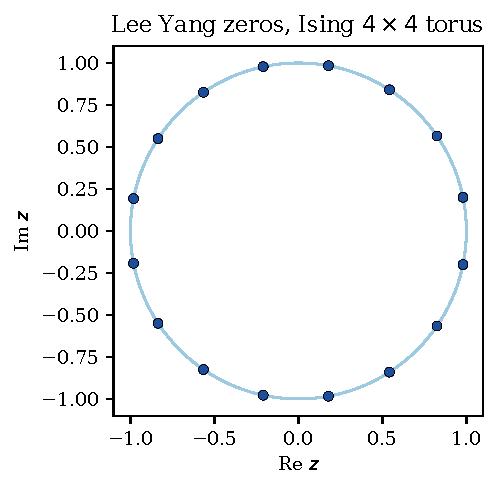
\includegraphics[width=0.62\textwidth]{lee_yang}
\caption{Lee Yang zeros of the Ising partition function on a $4\times4$ torus at $\beta J=0.6$, in the variable $z=e^{-2h}$. The largest value of $\big||z|-1\big|$ is $1.2\times10^{-15}$.}
\label{fig:lee_yang}
\end{figure}

Newman~\cite{newman1974} generalized the theorem to the ferromagnetic random variables of Chapter~\ref{ch:mixtures}, and for systems with this Lee Yang property the Griffiths, Hurst and Sherman inequality~\cite{griffiths1970}, which states that the magnetization is concave in a positive field, follows~\cite{newman1975}. In 1976 Newman~\cite{newman1976} reformulated the Riemann hypothesis in this language (Chapter~\ref{ch:open}).

\section{The Curie Weiss model and the Gaussian trick}\label{sec:curieweiss}

The mean field model has all pairs coupled with strength $1/N$:
\[
Z_N = \sum_{\sigma\in\{\pm1\}^N}\exp\Big(\frac{\beta}{2N}\Big(\sum_i\sigma_i\Big)^2+h\sum_i\sigma_i\Big).
\]
The quadratic interaction is decoupled by the Hubbard Stratonovich identity, which is the Gaussian integral $e^{a^2/2} = \E e^{aW}$ with $W\sim N(0,1)$, a scale mixture in reverse:
\[
\exp\Big(\frac{\beta}{2N}S^2\Big) = \sqrt{\frac{N\beta}{2\pi}}\int_\R\exp\Big(-\frac{N\beta m^2}{2}+\beta mS\Big)\dd m.
\]
Conditionally on $m$ the spins are independent, and summing over them gives
\begin{gather*}
Z_N = \sqrt{\frac{N\beta}{2\pi}}\int_\R\exp\big(-N\Psi(m)\big)\dd m, \\
\Psi(m) = \frac{\beta m^2}{2}-\log\big(2\cosh(\beta m+h)\big).
\end{gather*}
Laplace's method gives the free energy $-\lim N^{-1}\log Z_N = \min_m\Psi(m)$, attained where $\Psi'(m) = 0$, the mean field equation
\[
m = \tanh(\beta m+h).
\]
For $h = 0$ and $\beta\leq1$ the only solution is $m = 0$; for $\beta>1$ there are two symmetric minimizers $\pm m^*(\beta)$, and the magnetization jumps as $h$ crosses zero. The latent variable $m$ is a data augmentation: given $m$, the spins are independent with means $\tanh(\beta m+h)$, and given the spins, $m$ is Gaussian with mean $S/N$ and variance $1/(N\beta)$. The resulting two block Gibbs sampler is the Swendsen Wang idea in its simplest form, and the phase transition is visible as bimodality of the latent variable.

\section{Bayes optimal inference is a planted spin system}\label{sec:spiked}

Consider a signal $x^*\in\{\pm1\}^N$ drawn uniformly, and observations $Y_{ij} = \frac{\lambda}{N}x^*_ix^*_j+W_{ij}$ for $i<j$, with independent Gaussian noise of variance $1/N$, the spiked Wigner model. The posterior is
\[
p(x\mid Y)\propto\exp\Big(\lambda\sum_{i<j}Y_{ij}x_ix_j\Big),
\]
an Ising model with random couplings, a spin glass, whose couplings are correlated with a hidden planted configuration. Bayes optimal inference is statistical mechanics of this planted model, and the inverse temperature is fixed by the likelihood: it lies on what physicists call the Nishimori line.

\begin{theorem}[Nishimori identity]
Let $x^*\sim\pi$ take values in a standard Borel space, let $Y\mid x^*\sim p(\cdot\mid x^*)$, and, given $Y$, let $x$ and $x'$ be independent draws from the posterior $p(\cdot\mid Y)$, the conditional law of $x^*$ given $Y$, independent of $x^*$. For every bounded function $f$,
\[
\E\big[f(Y,x,x')\big] = \E\big[f(Y,x,x^*)\big].
\]
\end{theorem}

\begin{proof}
By definition of the posterior, conditionally on $Y$ the signal $x^*$ has the law $p(\cdot\mid Y)$, which is also the law of $x$ and of $x'$. Given $Y$ the three are independent. Hence $(Y,x,x^*)$ and $(Y,x,x')$ have the same law.
\end{proof}

The identity was introduced by Nishimori~\cite{nishimori1981} in 1981 for the Ising model with random bonds, using gauge transformations, and recognized in its statistical form by Iba~\cite{iba1999} and by Zdeborov\'a and Krzakala~\cite{zdeborova2016}. With a different prior or a different inverse temperature the draws are not draws from the conditional law of the signal given the data, and the identity fails in general. Taking $f(Y,x,x') = g\big(N^{-1}\langle x,x'\rangle\big)$ with $g$ bounded shows that the overlap between two posterior samples has the same law as the overlap between a posterior sample and the truth. This identity and the concentration of the overlap, which is proved separately, are the structural input of the proof of the replica symmetric formula for the mutual information by Lelarge and Miolane~\cite{lelarge2019}, who use the Aizenman Sims Starr scheme. The adaptive interpolation method of Barbier and Macris~\cite{barbier2019} gives another proof. Replica symmetry here means that the overlap has a single limiting value at equilibrium. It does not exclude metastable states, and it is compatible with the computational hardness discussed in the next section.

For the uniform sign prior of this section the replica symmetric formula for the mutual information per spin is
\[
\begin{multlined}\lim_{N\to\infty}\frac1NI(x^*;Y) = \min_{q\geq0}\Big\{\frac{\lambda^2}{4}(1-q)^2+\lambda^2q\\ -\E\log\cosh\big(\lambda^2q+\lambda\sqrt q\,\xi\big)\Big\},\end{multlined}
\]
where $\xi\sim N(0,1)$. The minimizer $q^*$ solves $q = \E\tanh(\lambda^2q+\lambda\sqrt q\,\xi)$ and is the limit of $|N^{-1}\langle x,x^*\rangle|$ for a posterior sample $x$. It vanishes for $\lambda\leq1$ and is close to $2(\lambda-1)$ just above $\lambda = 1$. The observation $\sqrt N\,Y_{ij} = \lambda\,x^*_ix^*_j/\sqrt N+\sqrt N\,W_{ij}$ is a Gaussian channel with signal to noise ratio $\lambda^2$ for the vector of products $(x^*_ix^*_j/\sqrt N)_{i<j}$, and $Y$ depends on $x^*$ only through these products. The I MMSE relation of Guo, Shamai and Verd\'u~\cite{guo2005}, Theorem~\ref{thm:immse} of Chapter~\ref{ch:entropy}, therefore gives
\begin{gather*}
\frac{\dd}{\dd(\lambda^2)}\frac1NI(x^*;Y) = \frac14\,\mathrm{mmse}_N, \\
\mathrm{mmse}_N = \frac{1}{N^2}\,\E\big\|x^*x^{*\top}-\E[x^*x^{*\top}\mid Y]\big\|_F^2.
\end{gather*}
Differentiating the replica symmetric formula gives $\mathrm{mmse}_N\to1-q^{*2}$, for all but countably many $\lambda$~\cite{lelarge2019}, so the phase transitions of the Bayes optimal error are read off from the minimizer $q^*$. For uniform signs the transition at $\lambda = 1$ is continuous. For other priors the error can jump. For sparse signals it jumps at the information theoretic threshold~\cite{lesieur2017}, and so does the optimal generalization error of the perceptron with binary weights~\cite{barbier2019b}.

\section{Statistical and computational thresholds}

The planted clique problem asks to find a clique of size $k$ planted in an Erd\H{o}s R\'enyi graph $G(n,\frac12)$. The largest clique in $G(n,\frac12)$ has size about $2\log_2n$, so a planted clique of size $k\geq(2+\varepsilon)\log_2n$ is identifiable by exhaustive search. Polynomial time algorithms are known only for $k\gtrsim\sqrt n$: spectral methods succeed for $k\geq C\sqrt n$~\cite{alon1998}, and Deshpande and Montanari~\cite{deshpande2015} showed that approximate message passing succeeds for $k\geq(1+\varepsilon)\sqrt{n/e}$, with the threshold $\sqrt{n/e}$ predicted by state evolution. Jerrum showed in 1992~\cite{jerrum1992} that from a suitable starting state the Metropolis process cannot find a planted clique of size $k = n^{1/2-\varepsilon}$ in polynomial time. The conjecture that no polynomial time algorithm succeeds for $k = n^{1/2-\varepsilon}$ is supported by lower bounds for sum of squares relaxations~\cite{barak2019} and for low degree polynomial tests~\cite{kunisky2019}, which have become a standard heuristic for computational hardness.

For Bayesian inference the lesson is that a posterior can be statistically informative and computationally inaccessible. The physical picture of the gap~\cite{zdeborova2016} is a phase transition in the landscape of the posterior: between the information theoretic and the algorithmic thresholds the posterior concentrates near the planted configuration, but a large, entropically dominant region of uninformative states separates any tractable starting point from it. A bottleneck of this kind makes the conductance of a reversible local dynamics, and with it the spectral gap and the log Sobolev constant of Chapter~\ref{ch:entropy}, exponentially small, so that Glauber or Langevin dynamics mixes slowly. This is a heuristic for hardness and not a general theorem. It has been proved for particular dynamics in particular models: the Metropolis process on the planted clique~\cite{jerrum1992}, and Langevin dynamics and gradient descent in tensor principal component analysis, where recovery from natural initializations takes at least stretched exponential time below an explicit threshold~\cite{benarous2020}. The heuristic concerns local dynamics and does not apply to spectral methods or approximate message passing. Obstructions for broader classes of algorithms come from other arguments, such as the overlap gap property~\cite{gamarnik2021}. In the physics of glasses equilibrium is likewise unattainable on accessible time scales. The analogy suggests that the gap is intrinsic, which remains a conjecture.

\section{Double descent as a phase transition}

Consider linear regression $y = X\theta+w$ with $n$ observations, $p$ isotropic Gaussian features, $\|\theta\|^2 = r^2$ and noise variance $\sigma^2$, in the proportional limit $p/n\to\psi$. Ridge regression with penalty $\alpha>0$ minimizes $n^{-1}\|y-X\theta\|^2+\alpha\|\theta\|^2$. The minimum norm least squares estimator, the limit of ridge regression as the penalty vanishes, has asymptotic prediction risk, by Hastie, Montanari, Rosset and Tibshirani~\cite{hmrt2022},
\[
R(\psi) = \begin{cases}\sigma^2\dfrac{\psi}{1-\psi}, & \psi<1,\\[2ex] r^2\Big(1-\dfrac1\psi\Big)+\dfrac{\sigma^2}{\psi-1}, & \psi>1.\end{cases}
\]
The risk diverges at the interpolation threshold $\psi = 1$ and then descends again, the double descent phenomenon. The divergence is a phase transition in the sense of this chapter: the smallest singular value of $X$ vanishes at $\psi = 1$, the Marchenko Pastur law reaching zero, and the inverse that defines the estimator blows up.

The Bayes posterior mean under the Gaussian prior with the correct signal and noise levels is ridge regression with penalty $\alpha = \sigma^2\psi/r^2$, and its risk is monotone in $\psi$ with no peak. Suppose instead that the penalty is held fixed while the number of features grows. The penalty corresponds to the working Gaussian prior $N(0,(\sigma^2/(n\alpha))I)$, which then no longer matches the signal. In our paper on Bayesian double descent~\cite{polsonsokolov2025dd} we show, for $\rho = r^2/\sigma^2$, that the limiting risk of ridge regression with fixed penalty $\alpha$ is nondecreasing in $\psi$ if and only if $\alpha\geq\alpha_c(\rho)$. The critical penalty $\alpha_c(\rho)$ is finite if and only if $\rho\geq1$, and $\alpha_c(2) = 1/11$. For $\alpha<\alpha_c(\rho)$ the risk has an interior maximum followed by a decreasing stretch, which is the double descent. Having more parameters than observations does not by itself produce the peak. It appears when the working prior is more diffuse than a critical level.

\section{Samplers from physics}

The Metropolis algorithm was invented at Los Alamos in 1953~\cite{metropolis1953} to compute the equation of state of a system of hard discs, the same system whose kinetic limit Lanford studied twenty years later. Glauber dynamics, heat bath updates of single spins, is the Gibbs sampler of statistics. Both suffer from critical slowing down near phase transitions, where the spectral gap closes.

Swendsen and Wang introduced in 1987~\cite{swendsen1987} a cluster algorithm that flips large clusters of aligned spins at once. Edwards and Sokal~\cite{edwards1988} explained it as data augmentation: introduce bond variables $\omega_{xy}\in\{0,1\}$ with joint law proportional to
\begin{gather*}
\prod_{\{x,y\}\in E}\Big((1-p)\mathbb{1}\{\omega_{xy} = 0\}+p\,\mathbb{1}\{\omega_{xy} = 1\}\mathbb{1}\{\sigma_x = \sigma_y\}\Big), \\
p = 1-e^{-2\beta J},
\end{gather*}
whose spin marginal is the Ising measure and whose bond marginal is the Fortuin Kasteleyn random cluster model. Given the spins, bonds are independent; given the bonds, clusters are assigned independent uniform spins. The algorithm is a two block Gibbs sampler on the augmented space, and it mixes rapidly at temperatures where single spin dynamics does not.

The slice sampler is the same idea in statistics: to sample a density $\pi(x)$, introduce $u\mid x\sim U(0,\pi(x))$ and sample $x\mid u$ uniformly on $\{\pi\geq u\}$. Damien, Wakefield and Walker~\cite{damien1999} developed it for Bayesian models, and Neal~\cite{neal2003} gave a general treatment. Augmentation can also fail. The witch's hat example of Polson in the discussion of Geyer's paper on practical Markov chain Monte Carlo~\cite{polson1992} exhibits a density, a narrow spike on a broad base, for which the Gibbs sampler and other local samplers appear to converge while missing a region of substantial mass; it is a phase coexistence problem in miniature, and it shows why diagnostics based on a single run cannot certify convergence. Rigorous complexity bounds for sampling log concave densities begin with the random walk algorithm of Dyer, Frieze and Kannan~\cite{dyer1991} for the uniform density on a convex body, which Applegate, Kannan and Polson~\cite{akp1990}, Applegate and Kannan~\cite{applegate1991} and Frieze, Kannan and Polson~\cite{frieze1994} extended to log concave densities. The analysis bounds the conductance of the walk, and through it the spectral gap, by isoperimetric inequalities of the kind proved for convex bodies by Lov\'asz and Simonovits~\cite{lovasz1993} and by Kannan, Lov\'asz and Simonovits~\cite{kannan1995}. These inequalities are quoted here without proof. Chapter~\ref{ch:poincare} relates the spectral gap to the Poincar\'e inequality and proves the inequality for the Gaussian measure, Theorem~\ref{thm:gaussian_poincare}.

\section{Onsager's solution and the critical point}\label{sec:onsager}

Onsager's 1944 solution~\cite{onsager1944} of the two dimensional Ising model on the square lattice with coupling $J$ and zero field gives the free energy per site
\[
\begin{multlined}-\beta f = \log2+\frac{1}{2\pi^2}\int_0^\pi\!\!\int_0^\pi\log\Big(\cosh^2(2\beta J)\\ -\sinh(2\beta J)\big(\cos k_1+\cos k_2\big)\Big)\dd k_1\dd k_2.\end{multlined}
\]
The integrand vanishes at $k_1 = k_2 = 0$ exactly when $\cosh^2(2\beta J) = 2\sinh(2\beta J)$, that is $\sinh(2\beta_cJ) = 1$, so the critical point is $\beta_cJ = \frac12\log(1+\sqrt2)\approx0.4407$, the value predicted earlier by Kramers and Wannier~\cite{kramers1941} from the duality between high and low temperature expansions. The specific heat diverges logarithmically at $\beta_c$. The spontaneous magnetization, announced by Onsager and proved by Yang in 1952~\cite{yang1952}, is
\[
m^*(\beta) = \big(1-\sinh^{-4}(2\beta J)\big)^{1/8},\qquad\beta>\beta_c,
\]
vanishing at $\beta_c$ with exponent $\frac18$. Mean field theory predicts the exponent $\frac12$, so the two dimensional model is a rigorous counterexample to the universality of mean field exponents. The exact solution showed for the first time that a phase transition with nonclassical exponents can follow from a microscopic model by pure mathematics, a demonstration of the derivational reading of the sixth problem in equilibrium statistical mechanics.

\section{The Gibbs variational principle and variational inference}

\begin{theorem}[Gibbs variational principle]
Let $\nu$ be a probability measure on a space $\Omega$ and $H:\Omega\to\R$ measurable with $Z = \int e^{H}\dd\nu<\infty$. Then
\[
\log Z = \sup_Q\Big\{\int H\dd Q-\KL(Q\,\|\,\nu)\Big\},
\]
the supremum over probability measures $Q$ with $\int|H|\dd Q<\infty$. If in addition $\int|H|e^{H}\dd\nu<\infty$, which is equivalent to $\KL(Q^*\,\|\,\nu)<\infty$, the supremum is attained, uniquely at $Q^*(\dd\omega) = Z^{-1}e^{H(\omega)}\nu(\dd\omega)$.
\end{theorem}

\begin{proof}
Let $Q$ be a probability measure with $\int|H|\dd Q<\infty$. If $Q$ is not absolutely continuous with respect to $\nu$, then $\KL(Q\|\nu) = \infty$ and the functional being maximized is $-\infty$. Otherwise $Q\ll Q^*$ and $\frac{\dd Q}{\dd Q^*} = Ze^{-H}\frac{\dd Q}{\dd\nu}$, so that $\KL(Q\|Q^*) = \KL(Q\|\nu)-\int H\dd Q+\log Z$. Hence $\int H\dd Q-\KL(Q\|\nu) = \log Z-\KL(Q\|Q^*)\leq\log Z$, with equality if and only if $Q = Q^*$. This gives the upper bound, the uniqueness, and the attainment whenever $Q^*$ is admissible, that is, whenever $\int|H|\dd Q^* = Z^{-1}\int|H|e^H\dd\nu<\infty$. In general let $Q_n$ be $Q^*$ conditioned on $\{|H|\leq n\}$. It is admissible, and the same computation gives $\int H\dd Q_n-\KL(Q_n\|\nu) = \log Z+\log Q^*(|H|\leq n)$, which tends to $\log Z$.
\end{proof}

The theorem is the Gibbs variational principle of statistical mechanics, in the form of the variational formula for relative entropy of Donsker and Varadhan~\cite{donsker1975}. With $\nu$ the prior, $H$ the log likelihood and $Q^*$ the posterior, it says that Bayes' rule is the solution of a variational problem and that the log marginal likelihood is a free energy. Restricting $Q$ to a tractable family gives a lower bound, the evidence lower bound of variational inference, whose gap is the Kullback Leibler divergence from the family to the posterior. Restricting to product measures gives mean field theory.

For the Curie Weiss model of Section~\ref{sec:curieweiss}, take $\nu$ uniform on $\{\pm1\}^N$ and $H_N(\sigma) = \frac{\beta}{2N}\big(\sum_i\sigma_i\big)^2+h\sum_i\sigma_i$, so that $Z_N = 2^N\int e^{H_N}\dd\nu$. The product measure $Q_m$ with mean $m$ at every site has $\KL(Q_m\|\nu) = N\big(\log2-s(m)\big)$, where $s(m) = -\frac{1+m}{2}\log\frac{1+m}{2}-\frac{1-m}{2}\log\frac{1-m}{2}$ is the binary entropy, and $\int H_N\dd Q_m = N\big(\frac{\beta m^2}{2}+hm\big)+\frac\beta2(1-m^2)$. The theorem therefore gives $N^{-1}\log Z_N\geq\varphi(m)$ for every $m\in[-1,1]$, where $\varphi(m) = \frac{\beta m^2}{2}+hm+s(m)$. This is not the function $-\Psi(m)$ of the Hubbard Stratonovich computation. Since $\log(2\cosh u) = \max_{m'}\{um'+s(m')\}$, attained at $m' = \tanh u$, we have $-\Psi(m) = \max_{m'}\{(\beta m+h)m'+s(m')\}-\frac{\beta m^2}{2}$. Taking $m' = m$ gives $-\Psi(m)\geq\varphi(m)$, with equality if and only if $m = \tanh(\beta m+h)$. Maximizing over $m$ first, which gives $\frac{\beta m'^2}{2}$, shows that $\max_m(-\Psi) = \max_{m'}\varphi$. The two functions thus have the same stationary points, the solutions of the mean field equation, and the same maximum, which is the limit of $N^{-1}\log Z_N$. For the Curie Weiss model the product bound is therefore sharp. Mean field theory in physics and variational Bayes in statistics are the same approximation, with the same failure mode: a product family cannot represent the correlations that dominate near a phase transition.

\section{Belief propagation and the Bethe approximation}

On a tree, marginals of a Gibbs measure can be computed exactly by passing messages along edges: the message from $x$ to $y$ summarizes the effect of the subtree behind $x$, and marginals are products of incoming messages. For the Ising model with fields $h_x$ and couplings $J_{xy}$, writing messages as effective fields $u_{x\to y}$, the update is
\[
u_{x\to y} = \operatorname{artanh}\Big(\tanh(\beta J_{xy})\tanh\Big(h_x+\sum_{z\sim x,z\neq y}u_{z\to x}\Big)\Big).
\]
On graphs with cycles the same iteration, loopy belief propagation, computes stationary points of the Bethe free energy~\cite{yedidia2005}, a variational approximation that is exact on trees and accurate on locally tree like graphs. Pearl introduced belief propagation for Bayesian networks in 1982~\cite{pearl1982}, Gallager had used it for decoding in 1963~\cite{gallager1963}, and the cavity method of M\'ezard, Parisi and Virasoro is its replica symmetric physics~\cite{mezard2009}. Approximate message passing~\cite{donoho2009,bayati2011}, used earlier in this chapter for the planted clique, is its dense graph limit, and its state evolution, a one dimensional recursion for the effective signal to noise ratio, is the mechanism by which algorithmic thresholds such as $\sqrt{n/e}$ are computed.

\section*{Exercises}
\begin{enumerate}
\item Solve the one dimensional Ising model on a ring by the transfer matrix method and show that there is no phase transition at positive temperature.
\item Verify directly that the zeros of the partition function of a single Ising bond in a uniform field lie on the unit circle.
\item Show that the Curie Weiss mean field equation with $h = 0$ and $\beta>1$ has three solutions, and determine which minimize $\Psi$.
\item Prove that the Edwards Sokal measure has the Ising measure as its spin marginal.
\item Show that ridge regression with penalty $\alpha$, the minimizer of $n^{-1}\|y-X\theta\|^2+\alpha\|\theta\|^2$, is the posterior mean under the prior $N(0,(\sigma^2/(n\alpha))I)$ and Gaussian noise of variance $\sigma^2$.
\end{enumerate}


\section*{Notes}

Friedli and Velenik~\cite{friedli2017} give a modern mathematical treatment of the Ising model, including the Peierls argument, correlation inequalities and the Lee Yang theorem. Zdeborov\'a and Krzakala~\cite{zdeborova2016} survey the statistical physics of inference. M\'ezard and Montanari's \emph{Information, Physics, and Computation}~\cite{mezard2009} develops message passing and the cavity method. Barbier and Macris~\cite{barbier2019c} give an introduction to the adaptive interpolation method for the Curie Weiss and Wigner spike models.

\chapter{Generative Bayesian Computation as Transport}
\label{ch:gbc}

\section{Bayes' rule as a map}

Bayes' rule is usually written as a statement about densities, $p(\theta\mid y)\propto p(y\mid\theta)p(\theta)$, and computed by Markov chain Monte Carlo, which needs the likelihood pointwise. In the problems of Parts~\ref{part:fluids} and~\ref{part:manifold} each evaluation of the likelihood is a forward solve of a partial differential equation, and for a stochastic simulator the density is not available at all. What is always available is the ability to simulate pairs $(\theta,y)$ from the joint law. Generative Bayesian computation (GBC)~\cite{polsonsokolov2025,polsonruggerisokolov2024} rewrites Bayes' rule as a statement about maps rather than densities: find a function $H$ such that $H(y,U)$, with $U$ a fixed reference noise, has the posterior law for every $y$. Learning $H$ from simulated pairs is a supervised problem, and once $H$ is learned, posterior sampling for any new $y$ costs one evaluation. Chapter~\ref{ch:manifold} applies the method to the inverse problem on the solution manifold of a partial differential equation.

\section{Noise outsourcing}

\begin{theorem}[Noise outsourcing]
\label{thm:outsourcing}
Let $(Y,\Theta)$ be random elements of standard Borel spaces. There is a measurable function $H$ such that $(Y,H(Y,U))$ has the law of $(Y,\Theta)$ whenever $U\sim U(0,1)$ is independent of $Y$. On a probability space that carries a uniform variable independent of $(Y,\Theta)$, there is moreover a $U\sim U(0,1)$ independent of $Y$ such that $\Theta = H(Y,U)$ almost surely.
\end{theorem}

\begin{proof}[Proof for real valued $\Theta$]
Let $F(\cdot\mid y)$ be a regular conditional distribution function of $\Theta$ given $Y = y$ and $H(y,u) = \inf\{t:F(t\mid y)\geq u\}$ its generalized inverse, the conditional quantile function. For $u\in(0,1)$ we have $H(y,u)\leq t$ if and only if $u\leq F(t\mid y)$, so $H(y,U)$ has distribution function $F(\cdot\mid y)$ when $U$ is uniform and independent of $Y$, which is the first claim. For the second, let $V$ be uniform and independent of $(Y,\Theta)$ and set $U = F(\Theta-\mid Y)+V\big(F(\Theta\mid Y)-F(\Theta-\mid Y)\big)$, the randomized probability integral transform. Conditionally on $Y = y$, $U$ is uniform, so $U$ is independent of $Y$, and $H(Y,U) = \Theta$ almost surely by the defining property of the quantile function. The general case reduces to this one by a Borel isomorphism with $[0,1]$.
\end{proof}

The theorem, a form of the transfer theorem of Kallenberg~\cite[Theorem~6.10]{kallenberg2002}, is the existence statement behind GBC. In several dimensions the map is not unique, and two canonical choices exist: the Knothe Rosenblatt map~\cite{rosenblatt1952,knothe1957} and the Brenier map of Theorem~\ref{thm:brenier}, which is optimal for quadratic cost.

\begin{lemma}[Check loss]
\label{lem:checkloss}
For $\tau\in(0,1)$ and integrable $\Theta$, the function $q\mapsto\E\rho_\tau(\Theta-q)$ with $\rho_\tau(r) = r(\tau-\mathbb{1}\{r<0\})$ is minimized by any $\tau$ quantile of $\Theta$. Consequently the minimizer over measurable $H$ of $\E\int_0^1\rho_\tau(\Theta-H(Y,\tau))\dd\tau$ is the conditional quantile function.
\end{lemma}

\begin{proof}
The function is convex in $q$ with right derivative $\P(\Theta\leq q)-\tau$, which changes sign at the $\tau$ quantile. The second claim follows by conditioning on $Y$ and minimizing pointwise in $(y,\tau)$.
\end{proof}

The check loss is a proper scoring rule for quantiles, so a flexible regression of simulated parameters on simulated data, with the quantile level as an additional input, learns the posterior quantile map. For vector parameters one can learn conditional quantiles of each coordinate given the data and the previous coordinates, which gives the Knothe Rosenblatt map, or learn a transport map directly. Every ordering of the coordinates gives an exact map when the conditional quantile functions are exact. When they are learned the ordering matters, because each stage conditions on coordinates generated by the earlier stages and their errors compound along the chain~\cite{nareklishvili2025review}.

\section{The Kalman filter as affine transport}

\begin{theorem}
\label{thm:kalman_transport}
Let $\theta\sim N(m,P)$ and $y = A\theta+v$ with $v\sim N(0,R)$ independent. Let $K = PA^\top(APA^\top+R)^{-1}$. If $(\theta',v')$ is an independent copy of $(\theta,v)$, then
\[
\theta'+K\big(y-A\theta'-v'\big)
\]
has, conditionally on $y$, the posterior law $N\big(m+K(y-Am),(I-KA)P\big)$.
\end{theorem}

\begin{proof}
The expression is affine in the Gaussian vector $(\theta',v')$, so it is Gaussian given $y$. Its mean is $m+K(y-Am)$ and its covariance is $(I-KA)P(I-KA)^\top+KRK^\top$, which equals $(I-KA)P$ by the definition of $K$, after expanding and using $K(APA^\top+R) = PA^\top$. These are the posterior moments.
\end{proof}

This is the perturbed observation form of the ensemble Kalman filter~\cite{evensen1994,burgers1998}: prior draws are transported to posterior draws by an affine map that uses the observation and fresh simulated noise. It is exact for linear Gaussian models, but it is a randomized coupling and not an optimal one. For $P = A = R = 1$ and $y = 0$ the gain is $K = 1/2$, the update sends $N(0,1)$ to the posterior $N(0,1/2)$ with a mean squared displacement of $1/2$, and the Brenier map between the same two laws, the deterministic map $x\mapsto x/\sqrt2$, has a mean squared displacement of $3/2-\sqrt2\approx0.086$. Outside the linear Gaussian case the affine update is a linear regression closure of Bayes' rule, and in general the ensemble Kalman filter does not converge to the Bayes posterior as the ensemble grows: for nonlinear state equations with linear observations its limit differs from the Bayes filter~\cite{legland2011}. GBC replaces the affine map by a learned nonlinear one.

\section{Optimal transport}

Given probability measures $\mu$ and $\nu$ on $\R^d$, Monge asked in 1781 for the map $T$ with $T_\#\mu = \nu$ that minimizes the mean distance $\int|x-T(x)|\,\mu(\dd x)$~\cite[Chapter~3]{villani2009}. The problem with the quadratic cost $\int|x-T(x)|^2\mu(\dd x)$ is the one solved by Brenier's theorem below. Kantorovich~\cite{kantorovich1942} relaxed the problem in 1942 to couplings, and the minimal quadratic cost over the couplings $\pi\in\Pi(\mu,\nu)$ is the squared Wasserstein distance of Chapter~\ref{ch:entropy}.

\begin{theorem}[Brenier]
\label{thm:brenier}
If $\mu$ is absolutely continuous and both measures have finite second moments, there is a unique optimal coupling, and it is induced by a map $T = \nabla\varphi$ with $\varphi$ convex, which is unique $\mu$ almost everywhere. Conversely, the gradient of any convex function pushing $\mu$ to $\nu$ is optimal.
\end{theorem}

We quote the theorem without proof. It is due to Brenier~\cite{brenier1991}, and Villani~\cite[Chapter~2]{villani2003} gives a proof. McCann~\cite{mccann1995} showed that a gradient of a convex function pushing $\mu$ to $\nu$ exists, and is unique $\mu$ almost everywhere, as soon as $\mu$ vanishes on Borel sets of Hausdorff dimension $d-1$, with no moment condition.

In one dimension the Brenier map and the Knothe Rosenblatt map coincide and equal $F_\nu^{-1}\circ F_\mu$, the quantile transform. GBC in one dimension is therefore optimal transport from uniform noise to the posterior. In several dimensions the two maps differ, and the Brenier map has the advantage of being independent of coordinates, and with a uniform reference law it defines a vector quantile function~\cite{carlier2016}; McCann's interpolation $((1-t)\mathrm{id}+tT)_\#\mu$~\cite{mccann1997} is the Wasserstein geodesic, along which displacement convex functionals such as entropy are convex.

\section{Diffusion models and Tweedie's formula}

Let $X_0\sim p_0$ and run the Ornstein Uhlenbeck process $\dd X_t = -X_t\dd t+\sqrt2\dd W_t$, whose law $p_t$ converges to the standard Gaussian. Anderson showed in 1982~\cite{anderson1982} that the time reversal $\bar X_s = X_{T-s}$ is again a diffusion,
\[
\dd\bar X_s = \big(\bar X_s+2\nabla\log p_{T-s}(\bar X_s)\big)\dd s+\sqrt2\dd\bar W_s.
\]
Starting from Gaussian noise at time $T$ and integrating backward with an estimate of the score $\nabla\log p_t$ produces approximate samples from $p_0$. This is the mechanism of diffusion based generative models. The score is learned by denoising score matching: since $X_t\mid X_0\sim N(e^{-t}X_0,(1-e^{-2t})I)$, the minimizer of
\[
\E\Big\|s(X_t,t)+\frac{X_t-e^{-t}X_0}{1-e^{-2t}}\Big\|^2
\]
over functions $s$ is $\nabla\log p_t$, by the following identity.

\begin{theorem}[Tweedie's formula]
\label{thm:tweedie}
Let $\theta\sim\pi$ and $y\mid\theta\sim N(\theta,\sigma^2I)$, with marginal density $p$. Then
\[
\E[\theta\mid y] = y+\sigma^2\nabla\log p(y).
\]
\end{theorem}

\begin{proof}
Write $g_\sigma(z) = (2\pi\sigma^2)^{-d/2}e^{-|z|^2/2\sigma^2}$, so that $p(y) = \int g_\sigma(y-\theta)\pi(\dd\theta)$ and $\nabla g_\sigma(z) = -z\,g_\sigma(z)/\sigma^2$. Since $|\nabla g_\sigma|$ is bounded, we may differentiate under the integral to get $\nabla p(y) = \int\frac{\theta-y}{\sigma^2}\,g_\sigma(y-\theta)\pi(\dd\theta)$. The posterior law of $\theta$ given $y$ is $g_\sigma(y-\theta)\pi(\dd\theta)/p(y)$, so dividing by $p(y)$ gives $\nabla\log p(y) = (\E[\theta\mid y]-y)/\sigma^2$.
\end{proof}

Robbins introduced the empirical Bayes idea in 1956~\cite{robbins1956} and Efron~\cite{efron2011} popularized Tweedie's formula in 2011 as a way to correct selection bias: the posterior mean depends on the prior only through the marginal density of the data, which can be estimated from the data themselves. Diffusion models are empirical Bayes at every noise level simultaneously. In one dimension the posterior mean is monotone in $y$, because $\frac{\dd}{\dd y}\E[\theta\mid y] = \Var(\theta\mid y)/\sigma^2\geq0$. A learned score need not respect this, and an estimated marginal need not be the marginal of any prior~\cite{dattapolson2025}. Monotonicity of the Tweedie posterior mean is equivalent to convexity of $y\mapsto\log p(y)+y^2/2\sigma^2$, which is a convex constraint on the log marginal, so an estimated score can be projected onto the set of scores that satisfy it.

\section{Schr\"odinger's bridge}

Return to Schr\"odinger's 1931 question from Chapter~\ref{ch:quantum}. Let $B$ be the law of Brownian motion with diffusion $\varepsilon$ on $[0,1]$, started from some reference law, and let $\mu,\nu$ be probability measures. The Schr\"odinger problem is
\[
\min\big\{\KL(Q\,\|\,B):Q\text{ a path measure with }Q_0 = \mu,\ Q_1 = \nu\big\}.
\]

\begin{theorem}[Static reduction]
\label{thm:static_reduction}
The problem reduces to the static problem
\[
\min\big\{\KL(\pi\,\|\,B_{01}):\pi\in\Pi(\mu,\nu)\big\},
\]
where $B_{01}$ is the joint law of the endpoints under $B$. If $\pi^*$ solves the static problem, the dynamic solution is $Q^* = \int B^{xy}\,\pi^*(\dd x,\dd y)$, a mixture of Brownian bridges $B^{xy}$ with the optimal endpoint law.
\end{theorem}

\begin{proof}
For any path measure $Q$, disintegrating with respect to the endpoints and using the chain rule for relative entropy,
\[
\KL(Q\|B) = \KL(Q_{01}\|B_{01})+\int\KL(Q^{xy}\|B^{xy})\,Q_{01}(\dd x,\dd y).
\]
The constraint involves only $Q_{01}$, and the second term is minimized, with value zero, by choosing the bridges $Q^{xy} = B^{xy}$.
\end{proof}

Since $B_{01}(\dd x,\dd y)\propto e^{-|x-y|^2/2\varepsilon}\,\dd x\,\dd y$ up to factors depending on $x$ alone, the static problem is entropic optimal transport,
\[
\min_{\pi\in\Pi(\mu,\nu)}\int\frac{|x-y|^2}{2}\,\pi(\dd x,\dd y)+\varepsilon\,\KL(\pi\,\|\,\mu\otimes\nu),
\]
whose solution has the form $\pi^*(\dd x,\dd y) = a(x)b(y)e^{-|x-y|^2/2\varepsilon}\mu(\dd x)\nu(\dd y)$. The functions $a,b$ solve the Schr\"odinger system, a pair of fixed point equations, and the iteration that alternately rescales rows and columns to match the marginals is Sinkhorn's algorithm~\cite{sinkhorn1964}, known in statistics as iterative proportional fitting and made a standard tool of machine learning by Cuturi~\cite{cuturi2013}. Chapter~\ref{ch:types} shows that each rescaling is an I projection, so that the iteration is a descent of relative entropy, and Section~\ref{sec:sinkhorn_hilbert} proves its geometric convergence by a different argument. Fortet proved the convergence of the iteration for the continuous problem in 1940, under regularity conditions on the kernel and the marginals~\cite{fortet1940}. If $\mu$ and $\nu$ have finite second moments, then as $\varepsilon\to0$ every weak limit point of the optimal entropic plans is an optimal plan for the quadratic cost, and the plans converge weakly to the optimal plan when $\mu$ is absolutely continuous, so that this plan is unique. This is a theorem of Mikami~\cite[Proposition~2.1]{mikami2004}, which L\'eonard~\cite{leonard2012} extended to a general class of reference processes and costs; the survey~\cite{leonard2014} gives the context. Figure~\ref{fig:sinkhorn} shows entropic plans for three values of $\varepsilon$: the plan sharpens from the independent coupling toward the monotone Brenier map.

\begin{figure}[t]
\centering
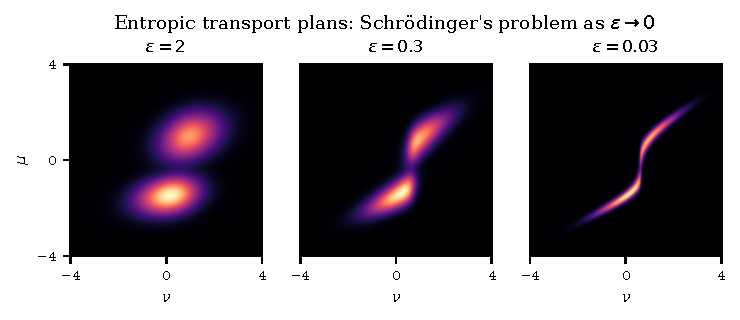
\includegraphics[width=\textwidth]{sinkhorn}
\caption{Entropic optimal transport plans between a bimodal law $\mu$ (vertical axis) and a Gaussian law $\nu$ (horizontal axis) on $[-4,4]$, computed by Sinkhorn iteration with the kernel $e^{-|x-y|^2/\varepsilon}$, so that the value of $\varepsilon$ in each panel title is twice the $\varepsilon$ of the formulas in the text. Brightness shows the square root of the mass of the plan in each cell, which brightens regions of small mass. As $\varepsilon$ decreases the plan concentrates on the graph of the monotone transport map.}
\label{fig:sinkhorn}
\end{figure}

The Sanov interpretation is Schr\"odinger's own~\cite{schrodinger1931}, in a heuristic form. Let $N$ independent Brownian particles start from the law $\mu$, and suppose that their empirical laws at times zero and one are observed to be close to $\mu$ and $\nu$, an event of exponentially small probability. Conditionally on it, the empirical measure of the paths converges to $Q^*$, first as $N\to\infty$ and then as the tolerance shrinks to zero, and so does the law of a single particle's path. The rigorous statement is a conditional law of large numbers on path space. It combines Sanov's theorem for empirical measures with a Gibbs conditioning principle of the kind proved for a finite alphabet in Chapter~\ref{ch:axioms}, and it needs hypotheses of its own. L\'eonard~\cite[Theorem~7.1]{leonard2010} proves a general conditional law of large numbers of this kind, and the survey~\cite[Section~6]{leonard2014} explains in outline how it applies to Schr\"odinger's problem. The Schr\"odinger bridge is the maximum entropy, equivalently most likely, explanation of an observed change of macroscopic state, which is the inferential sixth problem in its purest form: given two macroscopic snapshots, infer the microscopic dynamics that connects them. Score based diffusion models are the first iteration of an approximation of iterative proportional fitting for the Schr\"odinger bridge between the data law and Gaussian noise, and further iterations approach the bridge itself~\cite{debortoli2021}.

\section{Bootstraps and martingale posteriors}

Rubin's Bayesian bootstrap of 1981~\cite{rubin1981} assigns Dirichlet weights to the observations and treats the weighted empirical law as a draw from the posterior of the unknown distribution under a noninformative Dirichlet process prior. Newton and Raftery's weighted likelihood bootstrap~\cite{newtonraftery1994} extended this to parametric models, and our review with Lopes~\cite{weightedbootstrap2026} interprets the family of weighted bootstraps as generators: maps from random weights to parameter draws. Fong, Holmes and Walker~\cite{fongholmeswalker2023} proposed martingale posteriors, which replace the prior and likelihood by a sequence of one step ahead predictive distributions; the posterior is the law of the limiting parameter obtained by imputing the unobserved future observations from the predictive and refitting. When the predictive sequence is exchangeable, de Finetti's theorem (Theorem~\ref{thm:definetti}) makes it equivalent to a prior, and the martingale posterior is the conditional law of the de Finetti mixing measure given the data. Fong, Holmes and Walker require only that the sequence be conditionally identically distributed, a property studied by Berti, Pratelli and Rigo~\cite{berti2004} that is weaker than exchangeability. The predictive distributions then still converge almost surely to a random limit, but if the sequence is not exchangeable its law is not a mixture of independent and identically distributed laws, and no Bayesian model with independent and identically distributed observations generates it. Computing the martingale posterior by forward simulation is GBC with the generator defined by the predictive rule rather than learned from simulations.

\section{Quantile GBC for verifiable rewards}

Reinforcement learning with verifiable rewards trains a language model by sampling candidate solutions to a prompt from the current policy, scoring each with a verifier, and updating the policy toward the solutions that score well. For a fixed prompt and policy the reward is a random variable, and the construction of this chapter applies to it: simulate rewards from the policy and the verifier, learn the conditional quantile function of the reward by the check loss of Lemma~\ref{lem:checkloss}, and update the policy by a risk sensitive objective, such as a lower quantile of the reward, in place of its mean. We state this as a proposal. Whether it helps depends on the verifier. A binary verifier gives a Bernoulli reward with success probability $p$, whose quantile function $u\mapsto\mathbb{1}\{u>1-p\}$ takes only the values $0$ and $1$ and is determined by $p$, so quantiles of the reward carry no information beyond its mean. For graded rewards, such as partial credit or the combined scores of several verifiers, the quantile function carries more than the mean. For a binary verifier the uncertainty to quantify is the uncertainty about $p$, and GBC applies to it directly: with a $\mathrm{Beta}(a,b)$ prior and $k$ successes in $n$ independent samples the posterior is $\mathrm{Beta}(a+k,b+n-k)$, and its quantile function is the generator. The construction is that of the posterior generator of Chapter~\ref{ch:nsinference}, with the forward solve of the partial differential equation replaced by sampling from the policy and calling the verifier.

\section{A worked example: exact GBC for the normal model}

Let $\theta\sim N(0,\sigma_0^2)$ and $y\mid\theta\sim N(\theta,\sigma^2)$. The posterior is $N(by,b\sigma^2)$ with $b = \sigma_0^2/(\sigma_0^2+\sigma^2)$, and its quantile function is
\[
H(y,u) = by+\sqrt{b\sigma^2}\,\Phi^{-1}(u),
\]
where $\Phi$ is the standard normal distribution function. The map is affine in $y$ for each quantile level. A quantile regression of simulated $\theta_i$ on simulated $y_i$ with the check loss at level $u$, using linear functions of $y$, recovers $H$ exactly in the limit of many simulations; the error at sample size $N$ is of order $N^{-1/2}$ by standard quantile regression asymptotics. The efficiency of learning depends on how well the function class captures the conditional quantile function.

\section{Sinkhorn's algorithm and the Hilbert metric}
\label{sec:sinkhorn_hilbert}

Birkhoff's theory of positive operators gives a proof that Sinkhorn's iteration converges geometrically. For positive vectors define Hilbert's projective metric~\cite{hilbert1895}
\[
d_H(a,a') = \log\max_i\frac{a_i}{a'_i}+\log\max_j\frac{a'_j}{a_j},
\]
a metric on rays of the positive cone. Birkhoff showed in 1957~\cite{birkhoff1957} that a matrix $G$ with positive entries is a strict contraction for $d_H$, with contraction ratio $\tanh(\Delta/4)$, where $\Delta$ is the projective diameter of the image of the cone. Each half step of Sinkhorn's algorithm applies $G$ or $G^\top$ followed by a coordinatewise division, which is an isometry for $d_H$, so the scaling vectors converge geometrically, with ratio $\tanh^2(\Delta/4)$ per iteration. Franklin and Lorenz used this argument in 1989~\cite{franklinlorenz1989}. For the Gaussian kernel $G_{ij} = e^{-|x_i-y_j|^2/2\varepsilon}$ one finds $\log(G_{ik}G_{jl}/G_{il}G_{jk}) = (x_i-x_j)(y_k-y_l)/\varepsilon$ for rows $i,j$ and columns $k,l$, so that $\Delta = L_xL_y/\varepsilon$ for grids of diameters $L_x$ and $L_y$, and the ratio $\tanh(\Delta/4) = 1-O(e^{-\Delta/2})$ approaches one as $\varepsilon\to0$. The ratio is a worst case bound, and it is often far from sharp when the unregularized problem has a Monge map~\cite[Section~4.2]{peyrecuturi2019}, as it does in Figure~\ref{fig:sinkhorn}. There the grids span $[-4,4]$ and the ratio is within $10^{-13}$ of one in all three panels, yet the $\ell^1$ error of the marginals falls below $10^{-12}$ after about thirty, two hundred and two thousand iterations. The count grows in proportion to $1/\varepsilon$, in agreement with the local rate $1-\kappa$, $\kappa\sim\varepsilon$, that is observed numerically when a smooth Monge map exists~\cite[Section~4.2]{peyrecuturi2019}. Small regularization is therefore slow. Altschuler, Weed and Rigollet~\cite[Theorem~2]{altschuler2017} proved a polynomial bound: for a positive matrix with sum $s$ and smallest entry $m$, the iteration reaches an $\ell^1$ marginal error $\delta$ after $O(\delta^{-2}\log(s/m))$ steps, and $\log(s/m)$ grows like $1/\varepsilon$ for the Gaussian kernel.

\section{The F\"ollmer process and stochastic interpolants}

A simple bridge between a Dirac mass and a target law $\mu$ on $\R^d$ is the F\"ollmer process~\cite{follmer1985,lehec2013}: Brownian motion on $[0,1]$ started at zero and conditioned to have law $\mu$ at time one. It is the Schr\"odinger bridge from $\delta_0$ to $\mu$, its law is $\int B^{0y}\mu(\dd y)$ by Theorem~\ref{thm:static_reduction} with $\varepsilon=1$, where $B^{0y}$ is the Brownian bridge from zero to $y$, and its drift is
\[
b(t,x) = \nabla\log\E\Big[\frac{\dd\mu}{\dd\gamma}\big(x+\sqrt{1-t}\,Z\big)\Big],
\]
where $\gamma$ is the standard Gaussian law and $Z$ standard Gaussian. The process has the smallest relative entropy with respect to Wiener measure among all processes from zero to $\mu$, namely $\KL(\mu\|\gamma)$. Sampling by simulating the F\"ollmer process requires the drift, which can be estimated by Monte Carlo or learned. Stochastic interpolants~\cite{albergo2023} and flow matching~\cite{lipman2023} generalize the idea: one prescribes an interpolation $X_t = \alpha_tX_0+\beta_tX_1$ between noise and data, learns the conditional expectation of its velocity given its position by regression, and integrates the resulting ordinary or stochastic differential equation. The regression target is a conditional expectation, so the learning problem is again of the GBC type: simulate pairs, regress, and use the regression to transport noise to the target.

\section{Approximate Bayesian computation and its limits}

Approximate Bayesian computation, introduced by Tavar\'e, Balding, Griffiths and Donnelly~\cite{tavare1997} and by Pritchard and coauthors~\cite{pritchard1999} in the 1990s, accepts simulated parameters whose simulated summary statistics fall within a tolerance of the observed ones. In the limit of zero tolerance and sufficient summaries it is exact, but its accuracy degrades with the dimension $d$ of the summary: with $n$ simulations the minimal mean squared error of the estimated posterior density is of order $n^{-4/(d+5)}$, for rejection as for regression adjustment~\cite[Remark~1]{blum2010}. For a given accuracy the number of simulations then grows exponentially in $d$, up to constants that also depend on $d$. GBC removes the tolerance but not the dependence on dimension. The minimax rate for estimating a $p$ times differentiable regression function of $d$ variables is $n^{-p/(2p+d)}$ in $L^2$~\cite{stone1982}, and the conditional quantile function is no easier to learn, since in a location model every conditional quantile differs from the regression function by a constant. GBC therefore relies on structure in the quantile map and on a low dimensional summary statistic of the data. Regression adjustment, introduced by Beaumont, Zhang and Balding~\cite{beaumont2002} in 2002, corrects accepted parameters by a regression on the summaries and is a first order version of the quantile map. The progression from rejection to regression adjustment to learned generators parallels the progression in kinetic theory from direct simulation of particles to moment closures to learned surrogate models: each step replaces sampling by estimation of a conditional expectation.

\section*{Exercises}
\begin{enumerate}
\item Show that the minimizer of the check loss is unique when the distribution function is strictly increasing.
\item Verify the identity $(I-KA)P(I-KA)^\top+KRK^\top = (I-KA)P$.
\item Let $\mu$ have no atoms and let $T = F_\nu^{-1}\circ F_\mu$. (a) Show that $T_\#\mu = \nu$, and that $T$ is optimal for the quadratic cost when $\mu$ is absolutely continuous and both measures have finite second moments, using Theorem~\ref{thm:brenier}. (b) Let $c$ be convex. Show that $c(x-y)+c(x'-y')\leq c(x-y')+c(x'-y)$ for $x<x'$ and $y<y'$, and deduce that for $x_1<\dots<x_n$ and $y_1<\dots<y_n$ the matching $x_i\leftrightarrow y_i$ minimizes $\sum_ic(x_i-y_{\sigma(i)})$ over the permutations $\sigma$. (c) For $c(z) = |z|$, $\mu$ uniform on $[0,1]$ and $\nu$ uniform on $[1,2]$, show that every coupling has the same cost, so that $T$ is optimal but not unique.
\item Implement Sinkhorn's algorithm for two discrete measures on a grid and check that the marginal errors decrease geometrically. Estimate the rate per iteration for several values of $\varepsilon$ and compare it with $\tanh^2(\Delta/4)$, where $\Delta = L_xL_y/\varepsilon$ for the kernel $e^{-|x-y|^2/2\varepsilon}$ and grids of diameters $L_x$ and $L_y$.
\item Use Theorem~\ref{thm:tweedie} to compute the posterior mean when the prior is uniform on $\{-1,1\}$ and the noise is $N(0,\sigma^2)$.
\end{enumerate}


\section*{Notes}

Villani~\cite{villani2009} covers Brenier's theorem and the geometry of transport, and Peyr\'e and Cuturi~\cite{peyrecuturi2019} cover entropic transport and the computation of Sinkhorn's algorithm. L\'eonard~\cite{leonard2014} surveys the Schr\"odinger problem, its history and its relation to entropic transport. Song, Sohl Dickstein, Kingma, Kumar, Ermon and Poole~\cite{song2021} introduced the stochastic differential equation formulation of score based generative models in 2021. The noise outsourcing view of Bayesian computation is developed in our paper~\cite{polsonsokolov2025} and the quantile formulation for maximum expected utility in~\cite{polsonruggerisokolov2024}, and our review~\cite{nareklishvili2025review} places generative Bayesian computation among other classes of generators.

\chapter{Filters, Gates and Local Rules}
\label{ch:filters}

\section{Inference in real time}

A filter computes the posterior of a hidden state given observations up to the present, and updates it as each new observation arrives. Filtering is inference on the solution manifold performed sequentially, and it is also what any physical system that learns must do: a neuron, a thermostat, a trading algorithm or a language model processing a sequence holds a summary of the past and updates it recursively. The practical filters are approximations, either a Gaussian summary corrected by the score of the predictive density or a swarm of weighted samples. The stationary law of a neuron driven by Poisson input is a generalized Gamma convolution, which links the filter to the Thorin measures of Chapter~\ref{ch:mixtures}.

\section{Kalman, Bucy, Zakai}

For the linear Gaussian state space model $x_t = Fx_{t-1}+w_t$, $y_t = Hx_t+v_t$ with independent Gaussian noises $w_t\sim N(0,\Sigma_w)$ and $v_t\sim N(0,\Sigma_v)$, the filtering distribution is Gaussian, $x_t\mid y_{1:t}\sim N(m_t,P_t)$, and Kalman's recursion of 1960~\cite{kalman1960} gives
\begin{gather*}
m_t = Fm_{t-1}+K_t\big(y_t-HFm_{t-1}\big), \\
K_t = P_{t\mid t-1}H^\top\big(HP_{t\mid t-1}H^\top+\Sigma_v\big)^{-1},
\end{gather*}
with $P_{t\mid t-1} = FP_{t-1}F^\top+\Sigma_w$ and $P_t = (I-K_tH)P_{t\mid t-1}$. The Kalman Bucy filter of 1961~\cite{kalmanbucy1961} is the continuous time version, with the covariance solving a Riccati equation. For nonlinear diffusions observed in white noise,
\[
\dd X_t = b(X_t)\dd t+\sigma(X_t)\dd W_t,\qquad\dd Y_t = h(X_t)\dd t+\dd V_t,
\]
the unnormalized filtering density $q_t$ satisfies the Zakai equation of 1969~\cite{zakai1969},
\[
\dd q_t = \mathcal{L}^*q_t\dd t+q_t\,h\,\dd Y_t,
\]
a linear stochastic partial differential equation, where $\mathcal{L}^*$ is the Fokker Planck operator of the signal. The filter is a Fokker Planck flow tilted by the observations, the dynamic analogue of Bayes' rule, and it is infinite dimensional except in special cases. Particle filters, introduced by Gordon, Salmond and Smith in 1993~\cite{gss1993}, approximate it by a swarm of weighted samples that are propagated through the dynamics and resampled according to the likelihood.

\section{The score function filter}

Between the exact Kalman filter and the fully nonparametric particle filter lies a classical approximation.

\begin{theorem}[Score function update]
\label{thm:score_update}
Let $\theta\sim N(m,P)$ and let $y$ have conditional density $p(y\mid\theta)$, with marginal density $p_m(y) = \int p(y\mid\theta)N(\theta;m,P)\dd\theta$. Then
\begin{gather*}
\E[\theta\mid y] = m+P\,\nabla_m\log p_m(y), \\
\Var(\theta\mid y) = P+P\,\nabla_m^2\log p_m(y)\,P.
\end{gather*}
\end{theorem}

\begin{proof}
Since $\nabla_mN(\theta;m,P) = P^{-1}(\theta-m)N(\theta;m,P)$,
\[
\begin{aligned}\nabla_mp_m(y) &= P^{-1}\int(\theta-m)p(y\mid\theta)N(\theta;m,P)\dd\theta\\ &= P^{-1}\big(\E[\theta\mid y]-m\big)p_m(y).\end{aligned}
\]
Dividing by $p_m(y)$ gives the first identity. Differentiating once more gives the second.
\end{proof}

The theorem is Tweedie's formula of Chapter~\ref{ch:gbc} with the roles of prior and likelihood exchanged: the posterior mean is the prior mean plus the prior covariance times the score of the predictive density. Masreliez used it in 1975~\cite{masreliez1975} to build robust filters for heavy tailed observation noise, approximating the prior at each step by a Gaussian and computing the score of the non Gaussian predictive exactly. West's thesis and 1981 paper~\cite{west1981} developed the same idea for Bayesian forecasting with robust likelihoods.

\section{How Monte Carlo errors compound in particle filters}
\label{sec:pf_errors}

Each step of a particle filter adds Monte Carlo error, and the error of the next step is computed from an already approximate input. Whether these errors accumulate, and how fast, is the central question of sequential Monte Carlo. West~\cite{west1993} approximated posterior distributions by mixtures obtained by kernel smoothing of weighted samples, with the sequential updating of Monte Carlo approximations in view. Liu and West~\cite{liuwest2001} describe the difficulty that such updating brings, the degrading accuracy of particle representations updated over time, as particle attrition under resampling and weight degeneracy under reweighting. Doucet, Godsill and Andrieu~\cite{dga2000} gave a systematic treatment of sequential importance sampling and resampling, including the optimal proposal and the degeneracy of the weights.

\subsection{Weight degeneracy without resampling}

Consider sequential importance sampling without resampling for the hidden Markov model with transition density $p(x_s\mid x_{s-1})$ and likelihood $p(y_s\mid x_s)$. A path $x_{0:t}$ is drawn from a causal proposal, $x_0$ from its prior and $x_s\sim q_s(\cdot\mid x_{s-1},y_s)$ afterwards, and carries the weight $w_t = p(x_{0:t}\mid y_{1:t})/q(x_{0:t}\mid y_{1:t}) = \prod_{s\leq t}u_s$ with increments
\[
u_s = \frac{p(y_s\mid x_s)\,p(x_s\mid x_{s-1})}{q_s(x_s\mid x_{s-1},y_s)\,p(y_s\mid y_{1:s-1})}.
\]
Following Kong, Liu and Wong~\cite{klw1994} and Doucet, Godsill and Andrieu~\cite[Proposition~1]{dga2000}, we regard the observations as random variables with their true law, so that the weight is a function of the path and of the data and its variance is the unconditional variance. Let $\mathcal{F}_s$ be generated by $x_{0:s}$ and $y_{1:s}$. Given $\mathcal{F}_{s-1}$ the pair $(x_s,y_s)$ has density $q_s(x_s\mid x_{s-1},y_s)\,p(y_s\mid y_{1:s-1})$, and the integral of $u_s$ against this density over $x_s$ and $y_s$ is $\int p(x_s\mid x_{s-1})\dd x_s = 1$, provided the proposal is positive wherever the numerator of $u_s$ is. Hence $\E[u_s\mid\mathcal{F}_{s-1}] = 1$ and $(w_t)$ is a positive martingale with mean one.

\begin{proposition}[Kong, Liu and Wong]
\label{prop:klw}
Let $(w_t)$ be a positive square integrable martingale with $\E w_t = 1$ and increments $u_t = w_t/w_{t-1}$. Then the variance of the weight is nondecreasing in $t$:
\[
\Var(w_t) = \Var(w_{t-1})+\E\big[w_{t-1}^2\,\Var(u_t\mid\mathcal{F}_{t-1})\big]\geq\Var(w_{t-1}).
\]
If the increments are independent with $\E u_s^2 = 1+\sigma_s^2$ and $\sigma_s^2\geq\sigma^2>0$, then $\E w_t^2\geq(1+\sigma^2)^t$, with equality when $\sigma_s^2 = \sigma^2$ for all $s$, so the effective sample size $N/\E w_t^2$ decays at least geometrically.
\end{proposition}

\begin{proof}
By the martingale property, $\E w_t^2 = \E[w_{t-1}^2\E(u_t^2\mid\mathcal{F}_{t-1})] = \E[w_{t-1}^2(1+\Var(u_t\mid\mathcal{F}_{t-1}))]$, and subtracting $(\E w_t)^2 = 1 = (\E w_{t-1})^2$ gives the identity. If the increments are independent, then $w_{t-1}$ and $u_t$ are independent and $\E w_t^2 = \prod_{s\leq t}\E u_s^2 = \prod_{s\leq t}(1+\sigma_s^2)$.
\end{proof}

The effective sample size cannot increase, and in the model case of the proposition it reaches one after $\log N/\log(1+\sigma^2)$ steps, so that for any fixed $N$ the weights concentrate on a single path, and a larger $N$ postpones the collapse only in proportion to $\log N$. The increments of a hidden Markov model are not independent, but the left panel of Figure~\ref{fig:pf} shows the same geometric decay. It shows the effective sample size $(\sum_iW_i^2)^{-1}$ of the normalized weights $W_i$ for the local level model $x_t = x_{t-1}+\sqrt q\,\varepsilon_t$, $y_t = x_t+\sqrt r\,\nu_t$ with independent standard normal noise, $q = 0.1$, $r = 1$, $x_0\sim N(0,1)$ and $N = 1000$ particles. Without resampling it falls from $1000$ to about $180$ after ten steps, to about $26$ after twenty and to about $4$ after thirty, and it equals one to numerical precision after two hundred. With resampling at every step it stays above $350$.

\subsection{Errors with resampling}

Resampling resets the weights at the price of additional variance and of coalescing genealogies. The hidden state is a Markov chain with transition kernel $M$, and $\eta_1$ is the law of its first state. For a given sequence of observations, $g_t(x) = p(y_t\mid x)$ is the likelihood of the $t$th observation as a function of the state. Write $\eta_t = p(x_t\mid y_{1:t-1})$ for the predictive law, $\pi_t = p(x_t\mid y_{1:t})$ for the filter, $\mu(f) = \int f\dd\mu$, and $\Psi_t(\eta)(\dd x) = g_t(x)\,\eta(\dd x)/\eta(g_t)$ for the map that applies Bayes' rule to a prior $\eta$. Then $\pi_t = \Psi_t(\eta_t)$ and $\eta_{t+1} = \pi_tM = \Phi_t(\eta_t)$, where $\Phi_t(\eta) = \Psi_t(\eta)M$. The bootstrap filter with $N$ particles and multinomial resampling draws $X^1_1,\dots,X^N_1$ independently from $\eta_1$ and forms the empirical measure $\eta^N_t = \frac1N\sum_i\delta_{X^i_t}$ and the weighted measure $\pi^N_t = \Psi_t(\eta^N_t)$. It then draws $N$ ancestors from $\pi^N_t$ and moves each by $M$, so that, given the particles of step $t$, the particles of step $t+1$ are independent with law $\Phi_t(\eta^N_t)$.

\begin{theorem}[Del Moral; Crisan and Doucet; Del Moral and Guionnet]
\label{thm:pf_error}
Suppose that $a^{-1}\leq g_t\leq a$ for all $t$ and some $a\geq1$. Then for every $t$ there is a constant $c_t$ that does not depend on $N$ such that for every bounded $f$,
\[
\E\big|\eta_t^N(f)-\eta_t(f)\big|^2\leq\frac{c_t\,\|f\|_\infty^2}{N},
\]
and the same holds for $\pi_t^N(f)-\pi_t(f)$ with another constant. If in addition $\varepsilon\nu(A)\leq M(x,A)\leq\varepsilon^{-1}\nu(A)$ for all $x$ and all measurable $A$, for some probability $\nu$ and some $\varepsilon\in(0,1]$, then $c_t\leq4a^4\varepsilon^{-8}$ for every $t$: the filter forgets its errors, and the approximation is uniform in time.
\end{theorem}

\begin{proof}
Let $Q_s(x,\dd y) = g_s(x)M(x,\dd y)$, $Q_{s,t} = Q_s\cdots Q_{t-1}$ for $s<t$ and $Q_{t,t}$ the identity, so that $Q_{s,t}f(x)$ is the expectation of $f(X_t)\prod_{s\leq u<t}g_u(X_u)$ for the chain started at $X_s = x$. The exact flow from time $s$ to time $t$ is $\Phi_{s,t} = \Phi_{t-1}\circ\cdots\circ\Phi_s$, with $\Phi_{s,t}(\mu)(f) = \mu(Q_{s,t}f)/\mu(Q_{s,t}1)$ and $\Phi_{s,t}(\eta_s) = \eta_t$. Let $\mathcal{G}_s$ be the history of the particle system up to the particles of step $s$, and put $\bar\eta_1 = \eta_1$ and $\bar\eta_s = \Phi_{s-1}(\eta^N_{s-1})$ for $s\geq2$. Given $\mathcal{G}_{s-1}$ the measure $\eta^N_s$ is the empirical measure of $N$ independent draws from $\bar\eta_s$, and telescoping gives
\[
\eta^N_t(f)-\eta_t(f) = \sum_{s=1}^t\Big(\Phi_{s,t}(\eta^N_s)(f)-\Phi_{s,t}(\bar\eta_s)(f)\Big),
\]
a sum of local errors, the $s$th of which is the sampling error at step $s$ propagated to time $t$ by the exact flow. Write $G = Q_{s,t}1$, let $P_{s,t}f = Q_{s,t}f/G$, a Markov operator, and let $\lambda = \Phi_{s,t}(\bar\eta_s)(f)$. Since $\bar\eta_s(Q_{s,t}f-\lambda G) = 0$, the $s$th local error is
\[
\frac{(\eta^N_s-\bar\eta_s)\big(G\,(P_{s,t}f-\lambda)\big)}{\eta^N_s(G)}.
\]
The constant $\lambda$ is an average of $P_{s,t}f$, so $|P_{s,t}f-\lambda|\leq\omega_{s,t}$, the oscillation $\sup P_{s,t}f-\inf P_{s,t}f$, and $\eta^N_s(G)\geq\inf G$. Dividing by $\sup G\,\omega_{s,t}$ turns $G\,(P_{s,t}f-\lambda)$ into a function $h$ bounded by one, so the local error is at most $(\sup G/\inf G)\,\omega_{s,t}\,|(\eta^N_s-\bar\eta_s)(h)|$. Given $\mathcal{G}_{s-1}$, $(\eta^N_s-\bar\eta_s)(h)$ is the centered mean of $N$ independent variables bounded by one, with second moment at most $1/N$. The local error therefore has $L^2$ norm at most $(\sup G/\inf G)\,\omega_{s,t}\,N^{-1/2}$.

Under the first assumption $a^{-(t-s)}\leq G\leq a^{t-s}$, and $\omega_{s,t}\leq\mathrm{osc}(f)\leq2\|f\|_\infty$ because $P_{s,t}$ is a Markov operator, where $\mathrm{osc}(f) = \sup f-\inf f$. Minkowski's inequality then gives the first claim with $c_t = 4\big(\sum_{k<t}a^{2k}\big)^2$, which grows geometrically in $t$. Under the mixing assumption, $\sup G/\inf G\leq a^2\varepsilon^{-2}$ for $s<t$, because $G = g_sM(Q_{s+1,t}1)$ and $M(Q_{s+1,t}1)(x)$ varies by a factor of at most $\varepsilon^{-2}$ with $x$. Moreover $P_{s,t} = P_{s,s+1}\cdots P_{t-1,t}$ is a product of the Doob transformed kernels $P_{u,u+1}(x,\dd y) = M(x,\dd y)\,Q_{u+1,t}1(y)/M(Q_{u+1,t}1)(x)$, and each satisfies $P_{u,u+1}(x,\cdot)\geq\varepsilon^2\tilde\nu_u$ for all $x$, with $\tilde\nu_u(\dd y)\propto Q_{u+1,t}1(y)\,\nu(\dd y)$. By Dobrushin's contraction argument $\omega_{s,t}\leq(1-\varepsilon^2)^{t-s}\mathrm{osc}(f)$. The $L^2$ norm of the $s$th local error is then at most $a^2\varepsilon^{-2}(1-\varepsilon^2)^{t-s}\mathrm{osc}(f)\,N^{-1/2}$, and the sum over $s$ is at most $a^2\varepsilon^{-4}\mathrm{osc}(f)\,N^{-1/2}$. Finally $\pi^N_t(f)-\pi_t(f) = (\eta^N_t-\eta_t)\big(g_t(f-\pi_t(f))\big)/\eta^N_t(g_t)$ with $\eta^N_t(g_t)\geq a^{-1}$ and $\|g_t(f-\pi_t(f))\|_\infty\leq2a\|f\|_\infty$, so the bounds for $\eta^N_t$ carry over to $\pi^N_t$ with the constants multiplied by $4a^4$.
\end{proof}

The first assertion is the convergence result of Del Moral~\cite{delmoral1998} and of Crisan and Doucet~\cite{crisandoucet2002}, who require only that the likelihoods be bounded. Del Moral and Guionnet~\cite{delmoralguionnet2001} obtained bounds uniform in time, in $L^1$ and with the slower rate $N^{-\alpha/2}$ for some $\alpha<1$, under bounded likelihoods and an exponential stability condition on the filter. C\'erou, Del Moral and Guyader~\cite{cdg2011} state the rate $N^{-1/2}$ uniformly in $t$, as in the second assertion, under a regularity condition of the same kind, and refer to Del Moral's monograph~\cite{delmoral2004} for the convergence analysis of the occupation measures. The Gaussian likelihoods and kernels of the local level model of the figures do not satisfy these bounds, so the theorem describes the mechanism and does not cover that example.

The contraction that does the work in the theorem is a Dobrushin contraction of the Doob transformed kernels of the filter. It depends on the likelihoods as well as on the signal, and it is a different quantity from the spectral gap that governs Markov chain Monte Carlo in Chapter~\ref{ch:ergodic}.

\subsection{The likelihood estimator}

The particle filter also yields an unbiased estimator $\hat p_N(y_{1:t}) = \prod_{s\leq t}\eta^N_s(g_s)$ of the marginal likelihood, the product over time of the average unnormalized weights. Its relative variance compounds. C\'erou, Del Moral and Guyader~\cite{cdg2011} proved a nonasymptotic bound under a regularity condition: the ratio of the largest to the smallest value of each likelihood $g_s$ is at most $\delta$, and for some $m\geq1$ the $m$ step transition kernel satisfies $M^m(x,\cdot)\leq\beta M^m(x',\cdot)$ for all $x$ and $x'$. Under this condition, for $N>(t+1)\beta\delta^m$,
\[
\E\Big[\Big(\frac{\hat p_N(y_{1:t})}{p(y_{1:t})}-1\Big)^2\Big]\leq\frac{4(t+1)\beta\delta^m}{N}
\]
\cite[Corollary~5.2]{cdg2011}. The bound is of order $t/N$. B\'erard, Del Moral and Doucet~\cite{berard2014} showed that this order is correct. Let $t$ and $N$ tend to infinity with $t/N\to\alpha$. Under regularity and stability conditions of the same kind, $\log\hat p_N(y_{1:t})-\log p(y_{1:t})$ converges in law to a normal distribution with mean $-\alpha\sigma^2/2$ and variance $\alpha\sigma^2$, where $\sigma^2$ is a constant of the model. Pitt, Silva, Giordani and Kohn~\cite{pitt2012}, in a study of Markov chain Monte Carlo methods based on the particle filter, conjectured this lognormal limit and gave empirical evidence for it. The variance of the log likelihood estimator is therefore close to $\sigma^2t/N$, and keeping it bounded requires the number of particles to grow linearly with the length of the series. The middle panel of Figure~\ref{fig:pf} shows this for the local level model, where the exact likelihood is available from the Kalman filter: the variance of $\log\hat p_N-\log p$ grows roughly linearly in $t$, and increasing $N$ from $100$ to $1000$ reduces the slope by a factor of about ten.

\begin{figure}[t]
\centering
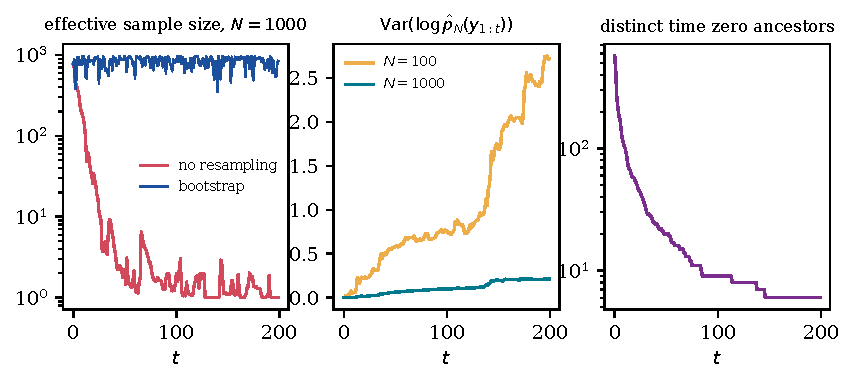
\includegraphics[width=\textwidth]{pf_errors}
\caption{Compounding of Monte Carlo error in particle filters for the local level model with $q = 0.1$ and $r = 1$. Left, effective sample size of the normalized weights for $N = 1000$ particles, with and without resampling. Middle, variance over sixty runs of the log likelihood estimate $\log\hat p_N(y_{1:t})$ for $N = 100$ and $N = 1000$, growing roughly linearly in $t$. Right, on a logarithmic scale, the number of distinct time zero ancestors among the $N = 1000$ resampled particles, the path degeneracy that afflicts smoothing and parameter learning.}
\label{fig:pf}
\end{figure}

\subsection{Path degeneracy and static parameters}

The right panel of Figure~\ref{fig:pf} shows the number of distinct ancestors at time zero of the particles alive at time $t$. It falls from $1000$ to about $570$ after one step, to $105$ after ten, to $20$ after fifty and to $6$ after two hundred. Resampling makes the genealogy coalesce. Two particles chosen at random at step $t$ have the same parent with probability $\sum_iW_i^2$, the inverse of the effective sample size, which is of order $1/N$. Koskela, Jenkins, Johansen and Span\`o~\cite{koskela2020} show, under strong conditions, that the genealogy converges to a Kingman coalescent when time is measured by the accumulated probability of such mergers, so that a single ancestor remains after a number of steps of order $N$. The filtering distribution at time $t$ can still be well approximated, as in Theorem~\ref{thm:pf_error}, but the approximation of the joint smoothing distribution of the whole path by the surviving genealogies is poor at early times. Godsill, Doucet and West~\cite{gdw2004} addressed this with backward simulation smoothing, which reuses the particle approximations of the filtering distributions at all times to draw whole trajectories backward in time, and so does not rely on the forward genealogy.

Static parameters are the worst case. A fixed parameter $\theta$ has no dynamics, so once the particle cloud in $\theta$ degenerates it never recovers, while in a regular model the posterior of $\theta$ keeps contracting at rate $t^{-1/2}$, and Monte Carlo error then dominates statistical error. The remedies developed since are ways of reintroducing dynamics or sufficient statistics: the kernel shrinkage method of Liu and West~\cite{liuwest2001}, which adds an artificial evolution to $\theta$ with the shrinkage rule of West~\cite{west1993} and a variance chosen to preserve the first two moments of the particle cloud; the sufficient statistic particle filters of Storvik~\cite{storvik2002} and of Carvalho, Johannes, Lopes and Polson~\cite{cjlp2010}, which carry conditional sufficient statistics for $\theta$ in each particle; the practical filter of Polson, Stroud and M\"uller~\cite{psm2008}, which approximates the posterior by a mixture of fixed lag smoothing distributions and uses sufficient statistics for the parameters without reweighting particles; and particle Markov chain Monte Carlo~\cite{adh2010}, which embeds the filter inside a Metropolis Hastings chain on $\theta$. Kantas and coauthors~\cite{kantas2015} survey the resulting methods.

\section{The particle filter as an interacting particle system}
\label{sec:pf_interacting}

The particle filter is not only an approximation to one posterior; it is a stochastic process whose time marginals converge, as the number of particles grows, to the predictive laws of the model, and whose reweighted particle clouds converge to the sequence of filtering posteriors. We use the notation of Section~\ref{sec:pf_errors}. Define, for each probability measure $\eta$, the McKean kernel $K_{t,\eta}(x,\cdot) = \Psi_t(\eta)M$, which does not depend on $x$ but depends on $\eta$: a particle at $x$ is replaced by a draw from the updated law and then moved. This is a nonlinear Markov chain in the sense of McKean, the discrete time analogue of the McKean Vlasov processes of Chapter~\ref{ch:kinetic}.

\begin{proposition}[The marginals are the posteriors]
\label{prop:pf_marginals}
Let $\bar X_1\sim\eta_1$ and, recursively, $\bar X_{t+1}\mid\bar X_t\sim K_{t,\mathrm{Law}(\bar X_t)}(\bar X_t,\cdot)$. Then $\mathrm{Law}(\bar X_t) = \eta_t$ for every $t$, and $\Psi_t(\mathrm{Law}(\bar X_t)) = \pi_t$. The time marginals of the nonlinear chain are therefore the predictive laws, and their Bayes updates are the filtering posteriors.
\end{proposition}

\begin{proof}
By induction. If $\mathrm{Law}(\bar X_t) = \eta_t$, then $\mathrm{Law}(\bar X_{t+1}) = \int\eta_t(\dd x)K_{t,\eta_t}(x,\cdot) = \Psi_t(\eta_t)M = \pi_tM = \eta_{t+1}$, and $\Psi_t(\eta_t) = \pi_t$ by Bayes' rule.
\end{proof}

Only the time marginals are asserted. The kernel $K_{t,\eta}(x,\cdot)$ does not depend on $x$, so the values $\bar X_1,\bar X_2,\dots$ are independent, and the law of the path of the chain is the product of the $\eta_t$, not a posterior for the path of the hidden state.

The bootstrap filter is the $N$ particle mean field approximation of this chain: each particle moves by $K_{t,\eta^N_t}$ with the unknown law replaced by the empirical measure $\eta^N_t$. Under the hypotheses of Theorem~\ref{thm:pf_error}, $\eta^N_t$ converges to the deterministic limit $\eta_t$. The particles are exchangeable, so Theorem~\ref{thm:sznitman} shows that the law of each particle at time $t$ converges to $\eta_t$ and that any $k$ particles become independent: the bootstrap filter propagates chaos. A single forward pass with $N$ particles, at cost $O(NT)$, thus delivers approximations to every intermediate posterior $p(x_t\mid y_{1:t})$, $t = 1,\dots,T$, not just the last one (upper panel of Figure~\ref{fig:pl}). Markov chain Monte Carlo, by contrast, targets one posterior at a time and must be rerun when a new observation arrives.

The resampling step selects, for each new particle, an ancestor index $a^i_t\in\{1,\dots,N\}$. These indices are discrete latent variables that switch at every step, and conditionally on the whole ancestry the particles move independently. The particle system is therefore itself a switching model on an extended space, with the ancestor indices as regimes; Andrieu, Doucet and Holenstein used this extended space construction to prove the exactness of particle Markov chain Monte Carlo~\cite{adh2010}. In continuous time the switching structure can be made part of the model itself (Section~\ref{sec:kurtz_xiong}). When the only latent state is a finite regime and the observation densities given the regime are known, the filter is exact and finite dimensional, Hamilton's filter~\cite{hamilton1989}, which is the forward algorithm for hidden Markov models of Section~\ref{sec:wonham}. When the state is linear and Gaussian given the path of the regime, each particle can carry the regime together with the Kalman mean and variance of the continuous state instead of a sampled value. This is the mixture Kalman filter of Chen and Liu~\cite{chenliu2000}, and by the Rao Blackwell inequality $\Var(\E[f\mid s])\leq\Var(f)$ it reduces the variance of the importance weights~\cite{dga2000}. The general principle is that a particle should carry the smallest summary of the past that makes the future conditionally tractable.

\section{Particle learning and conditional sufficient statistics}
\label{sec:particle_learning}

The principle applies to static parameters, where the naive particle filter fails. Suppose the model has parameter $\theta$ and that there are conditional sufficient statistics $s_t$, updated deterministically by
\[
s_{t+1} = S(s_t,x_t,x_{t+1},y_{t+1}),
\]
such that $p(\theta\mid x_{0:t},y_{1:t}) = p(\theta\mid s_t)$. This is the case in conditionally conjugate models, where the posterior of $\theta$ given the states and the data lies in a conjugate family with a sufficient statistic of fixed dimension. An example is the linear Gaussian state space model with unknown variances, treated below. Particle learning, introduced by Carvalho, Johannes, Lopes and Polson~\cite{cjlp2010}, tracks the essential state $z_t = (x_t,s_t,\theta)$ and updates it in a resample and propagate order:
\begin{enumerate}
\item Resample $\{z^i_t\}$ with weights proportional to the predictive likelihood $p(y_{t+1}\mid z^i_t) = \int p(y_{t+1}\mid x_{t+1},\theta)\,p(x_{t+1}\mid x_t,\theta)\dd x_{t+1}$.
\item Propagate $x^i_{t+1}\sim p(x_{t+1}\mid z^i_t,y_{t+1})$.
\item Update the sufficient statistics $s^i_{t+1} = S(s^i_t,x^i_t,x^i_{t+1},y_{t+1})$.
\item Draw $\theta^i\sim p(\theta\mid s^i_{t+1})$.
\end{enumerate}

\begin{proposition}[Exactness of the particle learning step]
\label{prop:pl_exact}
Let $z_t$ have the law $p(z_t\mid y_{1:t})$. Reweight this law by the predictive likelihood $p(y_{t+1}\mid z_t)$, which is step one at the level of laws, and then apply steps two to four. The new essential state $(x_{t+1},s_{t+1},\theta)$ has the law $p(x_{t+1},s_{t+1},\theta\mid y_{1:t+1})$.
\end{proposition}

\begin{proof}
By Bayes' rule, the reweighted law is $p(z_t\mid y_{1:t+1})\propto p(y_{t+1}\mid z_t)\,p(z_t\mid y_{1:t})$, since $y_{t+1}$ depends on the past only through $z_t$, and $p(x_{t+1}\mid z_t,y_{1:t+1}) = p(x_{t+1}\mid z_t,y_{t+1})$ by the Markov structure, which is step two. Hence after step two $(z_t,x_{t+1})$ has the law $p(z_t,x_{t+1}\mid y_{1:t+1})$, and $s_{t+1}$ is a deterministic function of it. It remains to show that $\theta$ redrawn in step four has the correct conditional law given $(x_{t+1},s_{t+1})$. Conditionally on the whole path $(x_{0:t+1},y_{1:t+1})$ the posterior of $\theta$ is $p(\theta\mid s_{t+1})$ by sufficiency. Since this depends on the path only through $s_{t+1}$, it is also the conditional law of $\theta$ given $(x_{t+1},s_{t+1},y_{1:t+1})$, by the tower property. Drawing $\theta$ afresh from it therefore leaves the joint law of $(x_{t+1},s_{t+1},\theta)$ equal to the posterior.
\end{proof}

The $N$ particle algorithm replaces the laws by empirical measures and the reweighting of step one by multinomial resampling, so it is an interacting particle approximation of this exact recursion. Two features distinguish particle learning from the naive filter. First, resampling uses the predictive likelihood before propagation, as in the auxiliary particle filter of Pitt and Shephard~\cite{pittshephard1999}, so particles are moved into regions supported by the new observation instead of being proposed blindly and then killed. Second, the parameter is redrawn at every step from its conditional posterior. The parameter cloud is therefore regenerated rather than inherited, and its values do not collapse onto the few distinct values that destroy the naive filter. What is inherited is the sufficient statistic, a deterministic function of the particle's path. It is subject to the path degeneracy of Section~\ref{sec:pf_errors}: particles that share an ancestor share the part of $s_t$ accumulated along the ancestral path. The essential state is also not mixing, since $s_t$ is a running sum and $\theta$ is static, so Theorem~\ref{thm:pf_error} gives no bound uniform in time for particle learning, and the Monte Carlo error of the parameter posterior can accumulate over long horizons. Chopin and coauthors~\cite{chopin2010} raised the potential for degeneracy in particle learning, related to the exponential forgetting of the past simulations, in their discussion of the method, while Carvalho, Johannes, Lopes and Polson~\cite{cjlp2010} report in simulations that the method is robust to degeneracy as the sample size grows.

\begin{example}[Local level model with unknown variances]
\label{ex:pl_local_level}
Let $x_t = x_{t-1}+\sqrt q\,\varepsilon_t$ and $y_t = x_t+\sqrt r\,\nu_t$, where $\varepsilon_t$ and $\nu_t$ are independent standard normal and $x_0\sim N(0,4)$, and let $q$ and $r$ have independent inverse Gamma priors $\mathrm{IG}(a_0,b_0)$, with density proportional to $\tau^{-a_0-1}e^{-b_0/\tau}$. The essential state is $z_t = (x_t,s^q_t,s^r_t,q,r)$ with sufficient statistics
\[
s^q_t = \sum_{u=1}^t(x_u-x_{u-1})^2,\qquad s^r_t = \sum_{u=1}^t(y_u-x_u)^2,
\]
and conditional posteriors $q\mid s_t\sim\mathrm{IG}(a_0+\frac t2,b_0+\frac12s^q_t)$ and $r\mid s_t\sim\mathrm{IG}(a_0+\frac t2,b_0+\frac12s^r_t)$. The predictive likelihood is $p(y_{t+1}\mid z_t) = N(y_{t+1};x_t,q+r)$, and the propagation density is Gaussian with variance $v = (q^{-1}+r^{-1})^{-1}$ and mean $v(x_t/q+y_{t+1}/r)$. Step one resamples with these explicit weights, and steps two to four are exact draws from known distributions.
\end{example}

Figure~\ref{fig:pl} applies particle learning with $N = 5000$ particles to $T = 400$ observations simulated with $q = 0.25$ and $r = 1$, with priors $\mathrm{IG}(3,1)$. The lower panels show the posterior medians and $90\%$ bands of $q$ and $r$ as functions of $t$, every one of which is a by product of the same run. They concentrate around the true values, with final medians $0.29$ and $1.01$. For comparison, a naive bootstrap filter with the same number of particles and the same data, which carries $(x_t,q,r)$ with the parameters fixed at their prior draws, ends with only three distinct values of $q$.

\begin{figure}[t]
\centering
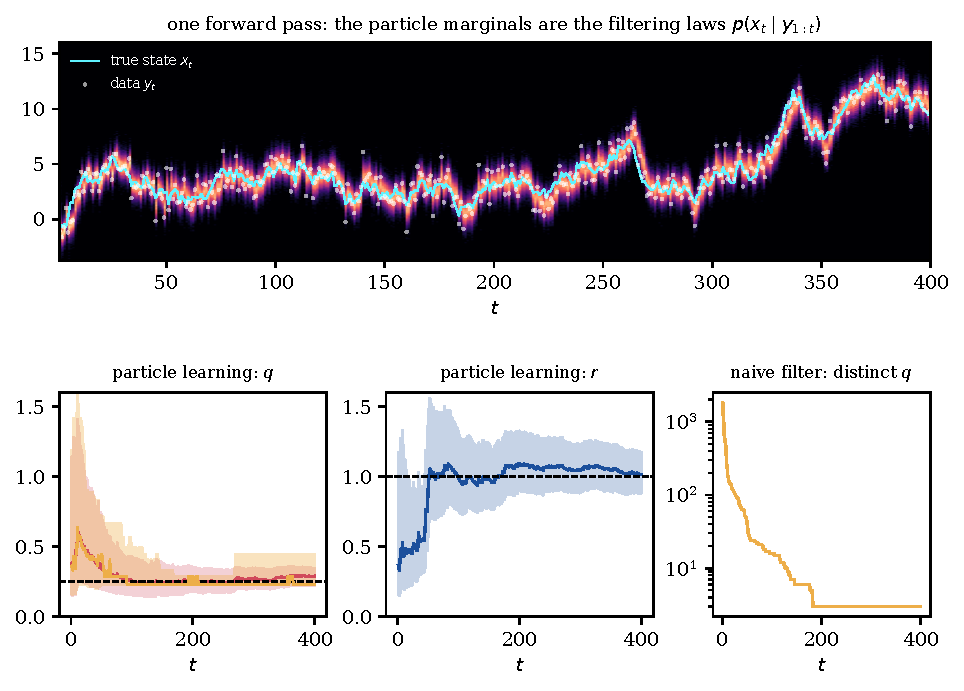
\includegraphics[width=\textwidth]{particle_learning}
\caption{Particle learning with $N = 5000$ particles for the local level model with unknown variances. Top, the particle histograms at each time from one forward pass, which are the filtering laws $p(x_t\mid y_{1:t})$, with the true state and the data. Bottom left and middle, sequential posterior medians and $90\%$ bands for $q$ and $r$, with the true values dashed; the lighter median and band at left are those of the naive filter for $q$. Bottom right, on a logarithmic scale, the number of distinct values of $q$ in the naive filter, which collapses to three.}
\label{fig:pl}
\end{figure}

Carvalho, Johannes, Lopes and Polson~\cite{cjlp2010} extend particle learning to smoothing by backward resampling, in the manner of Godsill, Doucet and West~\cite{gdw2004}, and to sequential model comparison through the predictive likelihoods computed in step one, whose running product is a particle estimate of the marginal likelihood. Carvalho, Lopes, Polson and Taddy~\cite{clpt2010} extend it to general mixtures and nonparametric mixtures. Its precursors are the sufficient statistic filters of Storvik~\cite{storvik2002} and Fearnhead~\cite{fearnhead2002}. In the language of this book, particle learning applies to filtering the lesson of the moment conditioning chapter, Chapter~\ref{ch:types}: carry the conditional sufficient statistics, the macroscopic variables, and let the remaining randomness be regenerated from its exact conditional law. In the language of de Finetti, when the observations are conditionally independent given $\theta$ the conditional sufficient statistic is the summary of the past through which the mixing variable $\theta$ is learned, and the particle carries the same summary in the presence of hidden states.


\section{Kurtz and Xiong: particle representations of filtering equations}
\label{sec:kurtz_xiong}

The particle filter is an algorithm, but it also suggests a theorem: the filtering distribution itself should be the limit of an interacting particle system, and the nonlinear filtering equations should be equations for the de Finetti measure of that system. Kurtz and Xiong made this precise~\cite{kurtzxiong1999}. They consider an infinite system of exchangeable particles $X_i(t)$ with weights $A_i(t)$, driven by individual Brownian motions $B_i$ and by a common noise $W$ shared by all particles, and interacting through their weighted empirical measure. A system of this kind has the form
\[
\begin{gathered}\dd X_i = \sigma(X_i,V)\dd B_i+b(X_i,V)\dd t+\alpha(X_i,V)\dd W,\\ \dd A_i = A_i\big(\beta(X_i,V)\dd t+\gamma(X_i,V)\cdot\dd W\big),\end{gathered}
\]
where the coefficients depend on the weighted empirical measure
\[
V(t) = \lim_{n\to\infty}\frac1n\sum_{i=1}^nA_i(t)\,\delta_{X_i(t)}.
\]
The limit exists because the particles are exchangeable, by de Finetti's theorem and the law of large numbers, and it is a random measure because the particles share the common noise $W$. Kurtz and Xiong show that $V$ is the unique solution of a nonlinear stochastic partial differential equation, and give conditions under which $V$ has an $L^2$ density with respect to Lebesgue measure. In the filtering application the common noise is the observation process and the weighted empirical measure is the filter. It is the unnormalized filter, which solves the linear Zakai equation, when the weights are the Kallianpur Striebel likelihood ratios, and the normalized filter, which solves the nonlinear Kushner Stratonovich equation, when the coefficients of the weights depend on $V$. For the filtering equation, uniqueness follows from uniqueness for the infinite particle system together with uniqueness for a corresponding linear stochastic partial differential equation~\cite[Chapter~7]{xiong2008}. With no common noise and constant weights the system reduces to the McKean Vlasov particle system of Chapter~\ref{ch:kinetic}, and $V$ is its deterministic limit.

The Kurtz Xiong representation closes a circle in this book. In Chapter~\ref{ch:axioms} propagation of chaos was a de Finetti statement: the empirical measure of an exchangeable system converges to a deterministic limit. In Chapter~\ref{ch:kinetic} that limit solved the Boltzmann or McKean Vlasov equation. Here the empirical measure converges to a random limit, because the particles share a common noise, and the limit solves a stochastic equation, the equation of the filter. The particle filter is a finite truncation of the Kurtz Xiong system with resampling in place of continuous weights, and its Monte Carlo error is the error of replacing a de Finetti limit by a finite empirical measure. Xiong's monograph~\cite{xiong2008} develops the filtering theory from this point of view, using the particle representation of the filter to prove uniqueness for the filtering equation and to construct numerical schemes~\cite[Chapters~7 and~8]{xiong2008}. Kurtz and Xiong~\cite{kurtzxiong2001} derived error bounds for such a simulation scheme that account for both the finite number of particles and the Euler discretization of the particle motions.

\subsection{Markov switching filtering equations}

The Kurtz Xiong representation extends to signals that switch between regimes. Give each particle, besides its position and weight, its own copy of a latent regime $z$ that mixes across processes, and let the coefficients of its motion and of its weight depend on that regime. When $z$ is static the result is a mixture of Kurtz Xiong systems. When $z$ is a Markov chain the result is a Markov switching system. Johannes, Polson and Stroud~\cite{jps2009} use particle filters for jump diffusion models of asset prices observed at discrete times, in which each particle carries the latent state variables.

Let $z_t$ be a Markov chain on $\{1,\dots,K\}$ with generator $Q = (Q_{jk})$, and let the signal and observation be
\[
\dd X_t = b(X_t,z_t)\dd t+\sigma(X_t,z_t)\dd B_t,\qquad\dd Y_t = h(X_t,z_t)\dd t+\dd W_t,
\]
where $B$ and $W$ are independent Brownian motions that are independent of $z$. For each regime $k$ let $\mathcal{L}_k f = b(\cdot,k)\cdot\nabla f+\frac12\tr(\sigma\sigma^\top(\cdot,k)\nabla^2f)$ be the generator of the signal frozen in regime $k$. The pair $(X_t,z_t)$ is a Markov process with generator
\[
\mathcal{L}f(x,k) = \mathcal{L}_kf(\cdot,k)(x)+\sum_jQ_{kj}\big(f(x,j)-f(x,k)\big).
\]

\begin{proposition}[Markov switching Zakai equation]
\label{prop:msw_zakai}
Let $b$ and $\sigma$ be Lipschitz and $h$ bounded, and let $\rho_t$ be the unnormalized conditional law of $(X_t,z_t)$ given $\mathcal{F}^Y_t$, defined by the Kallianpur Striebel formula, so that the Zakai equation $\dd\rho_t(f) = \rho_t(\mathcal{L}f)\dd t+\rho_t(hf)\dd Y_t$ holds for $f$ in the domain of $\mathcal{L}$. Write $\rho^k_t(\varphi) = \rho_t(\varphi\otimes\delta_k)$. Then for every $\varphi\in C^2_b(\R^d)$ and $k = 1,\dots,K$,
\[
\dd\rho^k_t(\varphi) = \Big(\rho^k_t(\mathcal{L}_k\varphi)+\sum_jQ_{jk}\,\rho^j_t(\varphi)\Big)\dd t+\rho^k_t\big(h(\cdot,k)\varphi\big)\dd Y_t.
\]
If $\rho^k_t$ has a density $q_t(\cdot,k)$ that is regular enough to integrate by parts, then $(q_t(\cdot,1),\dots,q_t(\cdot,K))$ solves the coupled system
\[
\begin{aligned}\dd q_t(\cdot,k) &= \Big(\mathcal{L}_k^*q_t(\cdot,k)+\sum_{j}Q_{jk}\,q_t(\cdot,j)\Big)\dd t\\ &\quad+h(\cdot,k)\,q_t(\cdot,k)\,\dd Y_t,\qquad k = 1,\dots,K,\end{aligned}
\]
where $\mathcal{L}_k^*$ is the formal adjoint of $\mathcal{L}_k$. The filtering distribution of the state is the mixture $\pi_t(\dd x) = \sum_kq_t(x,k)\dd x\big/\sum_k\int q_t(x',k)\dd x'$, and the regime probabilities are $\P(z_t = k\mid\mathcal{F}^Y_t) = \int q_t(x,k)\dd x\big/\sum_j\int q_t(x,j)\dd x$.
\end{proposition}

\begin{proof}
Apply the Zakai equation to $f(x,j) = \varphi(x)\delta_{jk}$. Because $\sum_lQ_{jl} = 0$, $\mathcal{L}f(x,j) = \delta_{jk}\mathcal{L}_k\varphi(x)+Q_{jk}\varphi(x)$. Hence $\rho_t(\mathcal{L}f) = \rho^k_t(\mathcal{L}_k\varphi)+\sum_jQ_{jk}\rho^j_t(\varphi)$ and $\rho_t(hf) = \rho^k_t(h(\cdot,k)\varphi)$, which is the first display. If $\rho^k_t$ has density $q_t(\cdot,k)$, then $\rho^k_t(\mathcal{L}_k\varphi) = \int\varphi\,\mathcal{L}_k^*q_t(\cdot,k)\dd x$ by integration by parts, which gives the coupled system. The last two statements are the Kallianpur Striebel normalization, $\pi_t(\varphi) = \sum_k\rho^k_t(\varphi)/\sum_k\rho^k_t(1)$.
\end{proof}

Each regime component evolves by its own Zakai equation, and the components exchange mass at the rates of the regime chain. This is the Markov switching stochastic partial differential equation. Its particle representation follows the Kurtz Xiong recipe with the regime added to the particle's state: particle $i$ carries $(X_i,Z_i,A_i)$, where $(X_i,Z_i)$ is an independent copy of the signal, with $Z_i$ a copy of the regime chain and $X_i$ moving with the coefficients of regime $Z_i$, and the weight evolves by $\dd A_i = A_i\,h(X_i,Z_i)\dd Y_t$. The weighted empirical measure
\[
V_t = \lim_{n\to\infty}\frac1n\sum_{i=1}^nA_i(t)\,\delta_{(X_i(t),Z_i(t))}
\]
equals $\rho_t$. Under the reference measure in which $Y$ is a Brownian motion independent of the signal, the triples $(X_i,Z_i,A_i)$ are independent given $Y$, and the Kallianpur Striebel formula gives $\E[f(X_i(t),Z_i(t))A_i(t)\mid Y] = \rho_t(f)$, so the limit exists and equals $\rho_t$ by the law of large numbers conditional on $Y$. After normalization by $V_t(1)$, its marginal on the regimes gives the regime filter and its marginal on the states gives the state filter. In discrete time, with resampling in place of continuous weights, it becomes a particle filter for a Markov switching model.

Figure~\ref{fig:msw} shows a two regime example in discrete time, with steps of length $0.05$ at which the particles are propagated, weighted and resampled as in the bootstrap filter. In regime zero the state drifts upward at rate one with volatility $0.6$, and in regime one it drifts downward at rate one with volatility $1.6$. The chain leaves regime zero at rate $0.15$ and regime one at rate $0.25$ per unit time, and the state is observed at every step with noise of standard deviation $0.3$. The lower panel shows the regime probability $\P(z_t = 1\mid y_{1:t})$, read off as the total weight of the particles in regime one. The filter classifies the regime correctly at $93\%$ of the steps. The path has two switches, and the filter registers them after $0.4$ and $0.65$ time units, a delay that accounts for about half of the misclassified steps. The rest are brief excursions of the filtered probability across one half, in both regimes.

\begin{figure}[t]
\centering
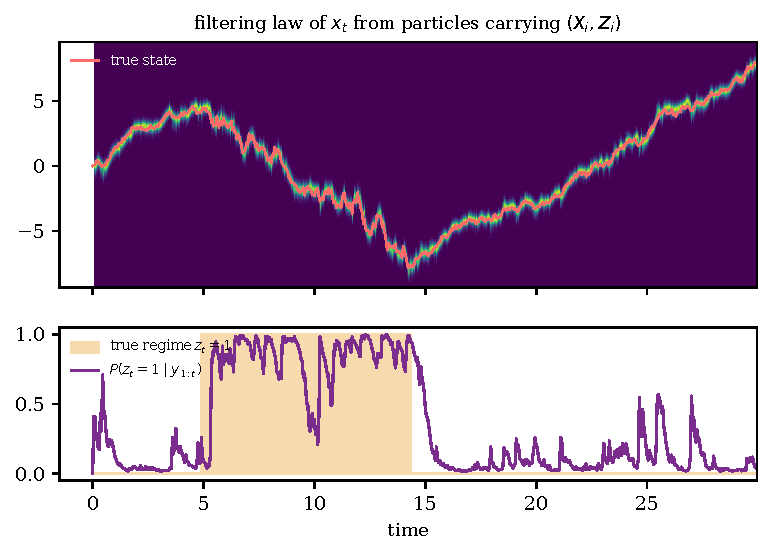
\includegraphics[width=0.95\textwidth]{markov_switching}
\caption{A Markov switching filter with $N = 4000$ particles, each of which carries its own latent regime chain. Top, the filtering law of the state with the true path. Bottom, the filtered regime probability against the true regime (shaded).}
\label{fig:msw}
\end{figure}


\section{Gates as approximate Bayes filters}
\label{sec:gates_bayes}

The long short term memory network (LSTM) of Hochreiter and Schmidhuber~\cite{hochreiter1997} carries a cell state $c_t$. In the form now in use, which includes the forget gate added by Gers, Schmidhuber and Cummins~\cite{gers2000}, the cell is updated by
\[
c_t = f_t\odot c_{t-1}+i_t\odot\tilde c_t,
\]
where $f_t$ and $i_t$, the forget and input gates, are sigmoid functions of the current input and previous hidden state, and $\tilde c_t$ is a candidate update. Compare the scalar Kalman filter for the random walk $x_t = x_{t-1}+w_t$ observed in noise, $y_t = x_t+v_t$, with $\Var(w_t) = q$ and $\Var(v_t) = r$:
\[
m_t = (1-K_t)\,m_{t-1}+K_t\,y_t,\qquad K_t = \frac{P_{t-1}+q}{P_{t-1}+q+r}.
\]
The gain is a logistic sigmoid, $K_t = 1/(1+e^{-u_t})$ with $u_t = \log\big((P_{t-1}+q)/r\big)$ the log signal to noise ratio. If the forget gate equals $1-K_t$, the input gate equals $K_t$ and the candidate is the observation $y_t$, the cell update is the Kalman update. In the Kalman filter the gain depends only on variances. In an LSTM it is a learned function of the input and the hidden state. The score function filter of Theorem~\ref{thm:score_update} lies between the two, with a gain that depends on the observation through the predictive score. Suppose the observation noise is a scale mixture of normals, as in Chapter~\ref{ch:mixtures}.

\begin{proposition}[The gain of the score function filter]
\label{prop:gates_bayes}
Let $\theta\sim N(m,P)$ and $y = \theta+v$, where $v\mid\lambda\sim N(0,r/\lambda)$ for a positive random variable $\lambda$ with law $\pi$ that is independent of $\theta$. Write $K_\lambda = P\lambda/(P\lambda+r)$ for the Kalman gain when the noise variance is $r/\lambda$. Then
\[
\E[\theta\mid y] = (1-K)\,m+K\,y,\qquad K = \E[K_\lambda\mid y]\in(0,1),
\]
and $\Var(\theta\mid y) = (1-K)P+(y-m)^2\Var(K_\lambda\mid y)$. The gain $K$ depends on $y$ only through $|y-m|$ and is nonincreasing in $|y-m|$. If $\lambda\equiv1$ then $K = P/(P+r)$.
\end{proposition}

\begin{proof}
Given $\lambda$ the model is linear Gaussian, so the Kalman update gives $\E[\theta\mid y,\lambda] = m+K_\lambda(y-m)$ and $\Var(\theta\mid y,\lambda) = (1-K_\lambda)P$. Averaging over the conditional law of $\lambda$ given $y$ gives the mean. The law of total variance gives $\Var(\theta\mid y) = \E[(1-K_\lambda)P\mid y]+\Var(m+K_\lambda(y-m)\mid y)$, which is the stated expression. Next, $y\mid\lambda\sim N(m,P+r/\lambda)$, so the conditional law $\mu_z$ of $\lambda$ given $|y-m| = z$ has density proportional to $(P+r/\lambda)^{-1/2}\exp\{-z^2/(2(P+r/\lambda))\}$ with respect to $\pi$, and it depends on $y$ only through $z$. For $z<z'$ the density of $\mu_{z'}$ with respect to $\mu_z$ is $g(\lambda)\big/\int g\dd\mu_z$ with $g(\lambda) = \exp\{-(z'^2-z^2)/(2(P+r/\lambda))\}$, which is decreasing in $\lambda$ because $P+r/\lambda$ decreases in $\lambda$. The gain $K_\lambda$ is increasing in $\lambda$. For two independent draws $\lambda,\lambda'$ from $\mu_z$ we have $(K_\lambda-K_{\lambda'})(g(\lambda)-g(\lambda'))\leq0$, and taking expectations gives Chebyshev's association inequality $\int K_\lambda g\dd\mu_z\leq\int K_\lambda\dd\mu_z\int g\dd\mu_z$. Hence $\int K_\lambda\dd\mu_{z'} = \int K_\lambda g\dd\mu_z\big/\int g\dd\mu_z\leq\int K_\lambda\dd\mu_z$.
\end{proof}

By Theorem~\ref{thm:score_update} the gain is the prior variance times the predictive score, divided by the innovation: $K = P\,\partial_m\log p_m(y)/(y-m)$. Each $K_\lambda = 1/(1+e^{-u})$ with $u = \log(P\lambda/r)$ is a logistic sigmoid of the log signal to noise ratio for noise variance $r/\lambda$, so the gate $K$ is a posterior average of sigmoids. It takes values in $(0,1)$, like an LSTM gate, and it falls as the innovation grows, because an observation far from the prediction is more likely to come from a large noise variance, and the filter then keeps more of its prior mean.

The proposition describes the gain of a filter, and the identification with an LSTM holds under conditions. The cell has the Kalman form $(1-K)m+Ky$ only when the gates are coupled, $f_t = 1-i_t$, the candidate is the observation and the output gate is ignored. The gain above is a function of the innovation alone, whereas an LSTM gate reads the input and the whole hidden state. The filter is itself an approximation. With scale mixture noise the exact filter is a mixture of Gaussians indexed by the past values of the mixing variable, and the score function filter keeps a single Gaussian with the mean and variance of the proposition. An LSTM can therefore be read as a learned approximation to this Bayes filter. Our paper on gates~\cite{polsonsokolov2026gates} develops the reading for the LSTM, the gated recurrent unit and the ARCH and GARCH models.

Autoregressive conditional heteroskedasticity has the same recursive form with a fixed gain. Engle's ARCH model~\cite{engle1982} and Bollerslev's GARCH model~\cite{bollerslev1986} estimate the variance of the next observation by
\[
\sigma^2_t = \omega+\alpha y^2_{t-1}+\beta\sigma^2_{t-1}.
\]
For $\beta<1$ iteration gives $\sigma^2_t = \omega/(1-\beta)+\alpha\sum_{j\geq1}\beta^{j-1}y^2_{t-j}$, an exponentially weighted average of past squared observations, and for $\omega = 0$ and $\alpha+\beta = 1$ it is $\sigma^2_t = (1-\alpha)\sigma^2_{t-1}+\alpha y^2_{t-1}$, the steady state update of the local level model of Section~\ref{sec:local_level} with gain $\alpha$. Read as a filter for the latent volatility of a stochastic volatility model, GARCH is therefore the analogue of the steady state Kalman filter and not of the gated filters, and Nelson~\cite{nelson1992} proved that, under conditions given in that paper, misspecified ARCH models are consistent filters for the volatility of diffusion processes in the continuous record limit.

\section{The shot noise neuron}

The leaky integrate and fire neuron has membrane potential obeying
\[
\tau\frac{\dd V}{\dd t} = -V+\tau\sum_kA_k\,\delta(t-t_k),
\]
where input spikes arrive at times $t_k$ with synaptic amplitudes $A_k$; in the subthreshold regime the potential is shot noise with the exponential pulse $e^{-t/\tau}\mathbb{1}_{t\geq0}$. Stein proposed this model of neuronal variability in 1965~\cite{stein1965}. Allowing each input its own time constant $\tau_k$, the potential at time $t$ is $V = \sum_{t_k\leq t}A_ke^{-(t-t_k)/\tau_k}$.

\begin{theorem}[Gamma law of the shot noise neuron]
\label{thm:shot_noise_neuron}
Let the input spikes form a Poisson process of rate $\lambda$ on $\R$. Attach to the $k$th spike a mark $(\tau_k,\kappa_k)$, the marks being independent with a common law $M$ on $(0,\infty)^2$ and independent of the spike times, and given the marks let the amplitude $A_k$ be exponential with rate $\kappa_k$. The stationary potential $V$ satisfies
\[
\begin{aligned}-\log\E e^{-\theta V} &= \lambda\int\tau\log\Big(1+\frac\theta\kappa\Big)M(\dd\tau,\dd\kappa)\\ &= \int\log\Big(1+\frac\theta y\Big)U(\dd y),\qquad\theta>0,\end{aligned}
\]
where $U$ is the image of the measure $\lambda\tau\,M(\dd\tau,\dd\kappa)$ under $(\tau,\kappa)\mapsto\kappa$. If $\int\log(1+1/y)\,U(\dd y)<\infty$, which is the condition that $U$ be a Thorin measure, then $V$ is a generalized Gamma convolution with Thorin measure $U$ and zero drift. Otherwise $V = \infty$ almost surely. In particular, if all marks equal $(\tau,\kappa)$ then $V$ has the Gamma law with shape $\lambda\tau$ and rate $\kappa$, and if $\tau_k$ and $\kappa_k$ are independent and $\kappa_k$ has law $\nu$ then $U = \lambda\E[\tau]\,\nu$.
\end{theorem}

\begin{proof}
Apply Campbell's theorem (Theorem~\ref{thm:campbell}) to the Poisson process of points $(s,\tau,\kappa,a)$, where $s = t-t_k>0$ is the age of the spike and $a$ its amplitude. Its intensity is $\lambda\dd s\otimes M(\dd\tau,\dd\kappa)\otimes\kappa e^{-\kappa a}\dd a$, and the function is $f = \theta ae^{-s/\tau}$. Integrating over $a$ first,
\[
\begin{aligned}-\log\E e^{-\theta V} &= \lambda\int M(\dd\tau,\dd\kappa)\int_0^\infty\Big(1-\frac{\kappa}{\kappa+\theta e^{-s/\tau}}\Big)\dd s\\ &= \lambda\int M(\dd\tau,\dd\kappa)\int_0^\infty\frac{\theta e^{-s/\tau}}{\kappa+\theta e^{-s/\tau}}\dd s\\ &= \lambda\int\tau\log\Big(1+\frac\theta\kappa\Big)M(\dd\tau,\dd\kappa),\end{aligned}
\]
using the substitution $w = \theta e^{-s/\tau}$ in the inner integral. The last expression is $\int\log(1+\theta/y)\,U(\dd y)$ by definition of $U$. Since $\min(1,\theta)\log(1+1/y)\leq\log(1+\theta/y)\leq\max(1,\theta)\log(1+1/y)$, it is finite for one $\theta>0$ if and only if it is finite for all, and then it is the Laplace exponent of a generalized Gamma convolution with Thorin measure $U$. Otherwise $\E e^{-\theta V} = 0$ for every $\theta>0$, which means $V = \infty$ almost surely. If all marks equal $(\tau,\kappa)$ then $U = \lambda\tau\,\delta_\kappa$, and the exponent $\lambda\tau\log(1+\theta/\kappa)$ is that of the Gamma law with shape $\lambda\tau$ and rate $\kappa$.
\end{proof}

The theorem gives a physical interpretation of Thorin measures: the Thorin measure of the stationary law of a leaky integrator driven by Poisson input is the distribution of the synaptic amplitude rates, weighted by the time constants. Time constants alone do not leave the Gamma family. With a common rate $\kappa$ a spread of time constants gives the Gamma law with shape $\lambda\E[\tau]$ and rate $\kappa$. A nontrivial generalized Gamma convolution needs a spread of amplitude rates, or a dependence between the rate and the time constant. Bondesson's shot noise representation, Theorem~\ref{thm:bondesson_shot}, is the same circuit read in the other direction. For a common time constant $\tau$ the ages of the spikes before time $t$ are the points $\Gamma_k/\lambda$ of a Poisson process of rate $\lambda$, with $\Gamma_k$ the points of a unit rate Poisson process, so the $k$th most recent spike contributes $E_ke^{-\Gamma_k/\beta}/\kappa_k$ to $V$, where $\beta = \lambda\tau$, $E_k$ is standard exponential and $\kappa_k\sim\nu$. This is the series of the theorem with Thorin measure $\beta\nu$. Every generalized Gamma convolution with zero drift and a Thorin measure $U$ of finite total mass $\beta$ is therefore the stationary potential of a neuron with a common time constant, $\lambda\tau = \beta$ and amplitude rates distributed as $U/\beta$. For a common time constant and amplitudes whose tail is completely monotone, that is, a mixture of exponentials, the stationary law lies in the Thorin class~\cite{polsonsokolov2026gbcshot}.

\section{Local learning rules}

Hebb proposed in 1949~\cite{hebb1949} that a synapse is strengthened when the presynaptic neuron repeatedly takes part in firing the postsynaptic one. In its simplest form $\Delta w = \gamma\,xa$ with postsynaptic activity $a = w^\top x$, the rule is unstable. Oja's modification of 1982~\cite{oja1982},
\[
\Delta w = \gamma\,a\,(x-aw),
\]
is a stochastic approximation (Section~\ref{sec:stoch_approx}) of the ordinary differential equation $\dot w = Cw-(w^\top Cw)w$ with $C = \E xx^\top$. Let $C$ be positive definite with eigenvalues $\ell_1>\ell_2\geq\dots\geq\ell_d>0$ and unit eigenvectors $v_1,\dots,v_d$, and write $w_i = v_i^\top w$. The equation reads $\dot w_i = (\ell_i-w^\top Cw)\,w_i$, so the ratio $w_i/w_1$ decays like $e^{-(\ell_1-\ell_i)t}$ and $w$ aligns with $\pm v_1$ whenever $w_1(0)\neq0$, while $\frac{\dd}{\dd t}|w|^2 = 2\,w^\top Cw\,(1-|w|^2)$ drives $|w|^2$ to one. The stable equilibria on the unit sphere are therefore the principal eigenvectors $\pm v_1$, and on the sphere the flow is the gradient ascent of the Rayleigh quotient. The rule is local in space, using only the activities of the two connected neurons and the weight itself, and it performs a global computation, principal component analysis, through the Robbins Monro mechanism of stochastic approximation~\cite{robbinsmonro1951}.

Crick argued in 1989~\cite{crick1989} that backpropagation is biologically implausible because it requires the transport of error signals backwards along axons, and much subsequent work has sought local rules that approximate gradient descent. A rule can be local in two senses. It is recursive if it updates a summary of the past using only the current observation and the previous summary, and it is local in space if each weight is updated from quantities available at its own synapse. Oja's rule is both. The Kalman filter and the gates of an LSTM are recursive but not local in space: the Kalman gain involves the covariance of the whole state and a matrix inversion, and a gate reads the whole hidden state. Crick's objection concerns locality in space. The filters of this chapter suggest a different framing of what a local rule can compute. Learning is filtering on parameters, and the question of which global computations can be carried out by recursive rules becomes the question of which posteriors admit finite dimensional recursive summaries. For a static parameter and independent observations the answer is the Pitman Koopman Darmois theorem~\cite{pitman1936,koopman1936,darmois1935}: under regularity conditions, and when the support of the observations does not depend on the parameter, a sufficient statistic of fixed dimension exists for every sample size only for exponential families. For a hidden state that evolves in time the classical finite dimensional filters are the few listed in Section~\ref{sec:wonham}, and beyond them the score function filter is an approximation.

\section{The energy budget}

The human brain consumes about twenty watts. Landauer's principle (Theorem~\ref{thm:landauer}) states that erasing one bit of unknown value at temperature $T$ dissipates at least $k_BT\log2$ of heat. At body temperature, $T = 310$ K, and with $k_B = 1.38\times10^{-23}$ J/K this is $2.97\times10^{-21}$ joules, so twenty watts could pay for at most $20/(2.97\times10^{-21})\approx6.7\times10^{21}$ bit erasures per second. Neurons are far from this limit. Levy and Calvert~\cite{levycalvert2021} estimate that the energy a neuron spends per bit of computation exceeds the physical minimum by a factor of about $10^8$. Any account of learning as physics, which is what the inferential sixth problem asks for, must include an account of the thermodynamic cost of updating beliefs. That is the subject of the next chapter.

\section{The local level model and the steady state gain}
\label{sec:local_level}

For the random walk plus noise model $x_t = x_{t-1}+w_t$, $y_t = x_t+v_t$, with $\Var(w_t) = q$ and $\Var(v_t) = r$, the Kalman recursion for the filtering variance is $P_t = \frac{(P_{t-1}+q)r}{P_{t-1}+q+r}$. Its fixed point solves $P^2+qP-qr = 0$, so
\[
P = \frac{-q+\sqrt{q^2+4qr}}{2},\qquad K = \frac{P+q}{P+q+r}.
\]
In steady state the filter is exponential smoothing, $m_t = (1-K)m_{t-1}+Ky_t$, and the gain depends only on the signal to noise ratio $q/r$. Muth showed in 1960~\cite{muth1960} that exponential smoothing is optimal for exactly this model, which explained the empirical success of a forecasting rule in use since the work of Brown and Holt in the 1950s~\cite{brown1959,holt2004,gardner1985} without a probabilistic justification. The example is the simplest case of the thesis of this chapter: a recursive update rule with a fixed gain is a Bayes filter for a particular model, and learning the gain from data is learning the signal to noise ratio.

\section{Hidden Markov models and the Wonham filter}
\label{sec:wonham}

When the hidden state is a Markov chain on a finite set with transition matrix $T$ and the observations have densities $p(y\mid j)$, the filter is the forward algorithm
\[
\pi_t(j)\propto p(y_t\mid j)\sum_i\pi_{t-1}(i)T_{ij},
\]
a finite dimensional recursion that is exact. Its continuous time version for a chain with generator $Q$ observed in white noise, $\dd Y_t = h(X_t)\dd t+\dd V_t$, is Wonham's filter~\cite{wonham1964},
\[
\dd\pi_t = Q^\top\pi_t\dd t+\big(\mathrm{diag}(h)-\langle h,\pi_t\rangle\big)\pi_t\,\big(\dd Y_t-\langle h,\pi_t\rangle\dd t\big),
\]
a nonlinear stochastic differential equation on the simplex driven by the innovation. The Wonham filter is the Kushner Stratonovich equation for a finite state space, and it is the second of the two classical cases, with the Kalman Bucy filter, in which the filter is finite dimensional. Bene\v{s} found a further class in 1981~\cite{benes1981} for nonlinear drifts satisfying a Riccati condition. Outside these cases the filter is infinite dimensional, and every practical method, extended Kalman filter, ensemble filter, particle filter, score function filter or learned recurrent network, is an approximation.

\section{Stochastic approximation and the ordinary differential equation method}
\label{sec:stoch_approx}

The Robbins Monro algorithm~\cite{robbinsmonro1951} $w_{n+1} = w_n+\gamma_n\big(h(w_n)+\xi_{n+1}\big)$ tracks the ordinary differential equation $\dot w = h(w)$ under three hypotheses: $h$ is Lipschitz, $\xi$ is a martingale difference sequence with $\E\big[|\xi_{n+1}|^2\mid\mathcal{F}_n\big]\leq C(1+|w_n|^2)$, and the step sizes satisfy $\sum\gamma_n = \infty$ and $\sum\gamma_n^2<\infty$. If the iterates are bounded almost surely, their limit set is internally chain transitive for the flow of the equation, by a theorem of Bena\"im~\cite{benaim1999}. If they return infinitely often to a compact subset of the domain of attraction of an asymptotically stable set of the equation, they converge to that set almost surely, by the theorem of Ljung~\cite{ljung1977} and of Kushner and Clark~\cite{kushnerclark1978}. Oja's rule, stochastic gradient descent and the online expectation maximization algorithm can be written in this form, with $h$ the mean update, and the hypotheses have to be checked in each case. The noise of Oja's rule is cubic in $w$, for example, so the bound on the second moment fails and boundedness of the iterates is an additional assumption.

With a small constant step $\gamma$, stochastic gradient descent $w_{n+1} = w_n-\gamma\big(\nabla L(w_n)+\zeta_{n+1}\big)$ on a loss $L$ is approximated, on the time scale $t = n\gamma$, by the diffusion $\dd w = -\nabla L(w)\dd t+\sqrt\gamma\,\Sigma(w)^{1/2}\dd B_t$, where $\Sigma(w)$ is the covariance of the gradient noise $\zeta$. If the noise is approximately Gaussian, independent of $w$ and isotropic, $\Sigma = s^2I$, the stationary density of the diffusion is proportional to $e^{-L/T}$ with $T = \gamma s^2/2$. Stochastic gradient descent then samples, approximately, from a Gibbs measure on the parameters at a temperature set by the learning rate, the picture of Mandt, Hoffman and Blei~\cite{mandt2017}, who tune the step size so that the stationary law matches a posterior. When the noise depends on $w$ or is anisotropic the stationary law is in general not $e^{-L/T}$. Chaudhari and Soatto~\cite{chaudhari2018} argue that for deep networks the noise is far from isotropic, that the stationary law is not the Gibbs measure of the loss, and that the most likely trajectories are closed loops. The temperature $T$ is a property of the algorithm. It is not the temperature of the heat bath in $k_BT\log2$, and the thermodynamic considerations of Chapter~\ref{ch:kolmogorov} concern the physical device that carries out the updates, not this effective temperature.

\section*{Exercises}
\begin{enumerate}
\item Derive the steady state Kalman gain for the local level model and show that it depends only on $q/r$.
\item Apply the score function update with a Gaussian prior and Student $t$ observation noise, for which the mixing variable $\lambda$ of Proposition~\ref{prop:gates_bayes} has a Gamma law, and plot the effective gain against the innovation.
\item Compute the mean and variance of the stationary voltage of the shot noise neuron with deterministic amplitudes.
\item Show that the fixed points of Oja's equation on the unit sphere are the unit eigenvectors of $C$. Show that when $C$ is positive definite and its largest eigenvalue is simple, only the top eigenvector, up to sign, is stable.
\item Write the forward algorithm for a two state hidden Markov model with Gaussian emissions.
\end{enumerate}


\section*{Notes}

Bain and Crisan's \emph{Fundamentals of Stochastic Filtering}~\cite{bain2009} covers the Zakai equation and particle filters. Gerstner and Kistler's \emph{Spiking Neuron Models}~\cite{gerstner2002} discusses the shot noise neuron, and shot noise processes with exponential kernel are treated in~\cite{polsonsokolov2026gbcshot}.

\chapter{Kolmogorov, Cybernetics and the Thermodynamics of Information}
\label{ch:kolmogorov}

\section{Kolmogorov in three roles}

Andrei Kolmogorov is among the mathematicians who appear most often in this book. He gave the axioms of probability in 1933~\cite{kolmogorov1933}, the forward and backward equations of diffusions in 1931~\cite{kolmogorov1931}, the theory of turbulence in 1941~\cite{kolmogorov1941a}, the traveling front of the Fisher equation in 1937~\cite{kolmogorov1937}, the superposition theorem that answered Hilbert's thirteenth problem in 1957~\cite{kolmogorov1957}, the invariant tori of perturbed Hamiltonian systems in 1954~\cite{kolmogorov1954}, and the algorithmic definition of information in 1965~\cite{kolmogorov1965}. He also thought hard about machines that learn. Wiener's \emph{Cybernetics}~\cite{wiener1948} appeared in 1948 and was denounced in the Soviet press as a bourgeois pseudoscience~\cite{gerovitch2002}; within a decade the political climate had changed. In 1961 Kolmogorov gave a lecture, \emph{Automata and Life}, which we read as arguing that there is no principled barrier to the construction of machines whose behavior is as complex as that of living beings, that the question of whether machines can think is a scientific question to be settled by the analysis of what thinking does rather than by definitions, and that the study of living systems and of automata should share a single mathematical language of information and control.

This chapter takes Kolmogorov's view seriously and asks what it means for the inferential sixth problem. If inference is a physical process, carried out by brains, by computers and by the scientific community, then it has a mechanics and a thermodynamics, and both are within the scope of Hilbert's request.

\section{The superposition theorem}

Hilbert's thirteenth problem asked whether the solution of the general equation of degree seven, as a function of its coefficients, can be written as a composition of continuous functions of two variables. A Tschirnhaus transformation reduces the equation to $x^7+ax^3+bx^2+cx+1 = 0$, so that only three parameters $a$, $b$, $c$ remain. Kolmogorov and Arnold, then Kolmogorov's student, answered a much stronger question in 1957~\cite{kolmogorov1957}.

\begin{theorem}[Kolmogorov superposition]
There exist continuous increasing functions $\phi_{q,p}:[0,1]\to\R$, for $q = 0,\dots,2n$ and $p = 1,\dots,n$, such that every continuous $f:[0,1]^n\to\R$ can be written as
\[
f(x_1,\dots,x_n) = \sum_{q=0}^{2n}g_q\Big(\sum_{p=1}^n\phi_{q,p}(x_p)\Big)
\]
for suitable continuous functions $g_q$ of one variable, depending on $f$.
\end{theorem}

The inner functions are universal; only the outer ones depend on $f$. Every continuous function of several variables is therefore a superposition of continuous functions of one variable and addition. We quote the theorem without proof; Braun and Griebel~\cite{braungriebel2009} give a constructive proof. The outer functions are continuous but not unique, and they can vary wildly even when $f$ is smooth~\cite{schmidthieber2021}. Arnold had shown earlier the same year~\cite{arnold1957} that every continuous function of three variables is a superposition of continuous functions of two variables, contradicting the answer Hilbert had expected.

The theorem has a long and somewhat contested history as a justification for neural networks: a network with two hidden layers of univariate nonlinearities can represent any continuous function exactly. The inner functions are rough: they are continuous and increasing, hence differentiable almost everywhere, but their graphs resemble that of the Cantor function~\cite{schmidthieber2021}, so exact representation says little about learnability, and Girosi and Poggio~\cite{girosipoggio1989} declared the theorem irrelevant for neural networks. But the structure, sums of univariate functions composed with univariate functions, is that of generalized additive models, and Kolmogorov Arnold networks~\cite{liu2024kan} with smooth learned univariate pieces are a practical descendant. For the themes of this book the important point is different: Kolmogorov showed that the apparent complexity of a high dimensional function can be reduced, without loss, to a small number of one dimensional operations arranged in the right architecture. The search for such architectures is the search for representations in which inference is easy.

\section{Algorithmic information}

Recall from Chapter~\ref{ch:axioms} the prefix Kolmogorov complexity $K(x)$ of a finite string. It is uncomputable but approximable from above, invariant up to an additive constant, and connected with Shannon entropy by the theorem that for independent samples from a computable law $P$,
\[
\frac1n\E K(X_1,\dots,X_n)\to H(P).
\]
The universal prior $m(x)\approx2^{-K(x)}$ dominates every computable prior, so Bayesian prediction with $m$ incurs total log loss at most $K(P)\log2$ more than prediction with the true $P$. Rissanen's minimum description length principle~\cite{rissanen1978} and its refinements are practical versions: choose the model that gives the shortest two part code for the data, the description of the model plus the description of the data given the model. For regular parametric families with a $d$ dimensional parameter $\theta$ the two part code length is
\[
-\log p(x_{1:n}\mid\hat\theta)+\frac d2\log n+O(1),
\]
which is half the Bayesian information criterion. The refined code length, the stochastic complexity of Rissanen~\cite{rissanen1996}, is
\[
-\log p(x_{1:n}\mid\hat\theta)+\frac d2\log\frac n{2\pi}+\log\int\sqrt{\det J(\theta)}\dd\theta+o(1),
\]
where $J$ is the Fisher information matrix and the integral runs over a compact parameter set. It agrees to $o(1)$ with the negative log marginal likelihood under Jeffreys' prior. Occam's razor, Bayesian model selection and compression are one principle.

\section{Maxwell's demon}

In a letter to Tait in 1867, and in the \emph{Theory of Heat} of 1871~\cite{maxwell1871}, Maxwell imagined a being who controls a trapdoor between two chambers of gas and lets only fast molecules pass one way and slow ones the other, creating a temperature difference without work, in apparent violation of the second law. For sixty years the demon resisted exorcism. Smoluchowski argued in 1912~\cite{smoluchowski1912} that thermal fluctuations of any mechanical trapdoor would defeat it. The decisive analysis began with Szilard in 1929~\cite{szilard1929}.

Szilard reduced the demon to its information theoretic core: a single molecule in a box of volume $V$ in contact with a heat bath at temperature $T$. A partition is inserted in the middle, the demon observes which half the molecule is in, attaches a piston on the empty side, and lets the molecule push the piston isothermally back to volume $V$. The work extracted is
\[
W = \int_{V/2}^{V}\frac{k_BT}{v}\dd v = k_BT\log2.
\]
One bit of information about the molecule's position converts into $k_BT\log2$ of work from a single heat bath. If the demon could repeat the cycle indefinitely, the second law would fail; therefore, Szilard argued, acquiring or handling the bit must cost at least $k_BT\log2$ of dissipation.

Szilard located the cost in the measurement. Landauer in 1961~\cite{landauer1961} located it elsewhere: logically irreversible operations, such as erasing a bit of unknown value to reset a memory, must dissipate at least $k_BT\log2$ per bit, because they compress the phase space of the memory and must export the corresponding entropy to the environment. Bennett in 1982~\cite{bennett1982} completed the argument by showing that measurement can be done reversibly, so the demon's unavoidable cost is the erasure of its memory at the end of each cycle, which exactly compensates the work extracted. B\'erut and coauthors confirmed Landauer's bound experimentally in 2012~\cite{berut2012} with a colloidal particle in a double well potential, observing that the mean dissipated heat approaches $k_BT\log2$ in the limit of slow erasure.

\begin{theorem}[Landauer bound, information theoretic form]\label{thm:landauer}
Let a memory with finitely many states of equal energy and a heat bath at temperature $T$ be initially independent, the memory having the distribution $p$ and the bath being in its Gibbs state at temperature $T$. Let the memory and the bath then evolve together under reversible dynamics, Hamiltonian or unitary, possibly driven by a protocol fixed in advance, until the memory has the distribution $q$, and let $Q$ be the energy gained by the bath. Then
\[
\E Q\geq k_BT\big(H(p)-H(q)\big)\log2,
\]
with entropies in bits. In particular erasing a uniformly random bit, $H(p) = 1$, $H(q) = 0$, dissipates at least $k_BT\log2$.
\end{theorem}

\begin{proof}
Measure entropy in units of $k_B$. The memory then has entropy $H(p)\log2$ when its distribution is $p$, and we write $S(\pi)$ for the entropy of the bath in the state $\pi$. Reversible dynamics conserve the entropy of the joint state. Initially the joint state is a product, with entropy $H(p)\log2+S(\pi_0)$, where $\pi_0\propto e^{-\mathcal H_B/k_BT}$ is the Gibbs state of the bath with Hamiltonian $\mathcal H_B$. Finally the entropy of the joint state is at most the sum $H(q)\log2+S(\pi_1)$ of the entropies of its marginals, where $\pi_1$ is the final state of the bath. Hence $S(\pi_1)-S(\pi_0)\geq(H(p)-H(q))\log2$. On the other hand, writing out $\KL(\pi_1\|\pi_0)\geq0$ for the Gibbs state $\pi_0$ gives $S(\pi_1)-S(\pi_0)\leq(\E_{\pi_1}\mathcal H_B-\E_{\pi_0}\mathcal H_B)/k_BT = \E Q/k_BT$. The two bounds together give the claim.
\end{proof}

The bound is the exchange rate between information and energy, and it is the thermodynamic content of the inferential sixth problem.

\section{Kelly: information as growth}

In 1956 John Kelly, at Bell Laboratories, gave Shannon's information rate an economic interpretation~\cite{kelly1956}. A gambler bets repeatedly on a binary event of probability $p>\frac12$ at even odds, wagering a fraction $f$ of capital on the favored outcome. The capital after $n$ bets is $B_n = B_0\prod_{i=1}^n(1+fs_i)$, with $s_i = +1$ if bet $i$ is won and $s_i = -1$ if it is lost, and its exponential growth rate is
\[
G(f) = \lim_n\frac1n\log_2\frac{B_n}{B_0} = p\log_2(1+f)+(1-p)\log_2(1-f).
\]

\begin{theorem}[Kelly]\label{thm:kelly}
$G$ is maximized at $f^* = 2p-1$, and $G(f^*) = 1-H(p)$ bits per bet, where $H(p) = -p\log_2p-(1-p)\log_2(1-p)$. More generally, for a horse race with win probabilities $p_i$ and odds $o_i$, meaning that a unit bet on horse $i$ returns $o_i$ if it wins, with $\sum1/o_i = 1$, betting the fraction $b_i$ of wealth on horse $i$ gives growth rate
\[
G(b) = \sum_ip_i\log_2(b_io_i) = \KL(p\,\|\,r)-\KL(p\,\|\,b),\qquad r_i = 1/o_i,
\]
maximized by proportional betting $b = p$.
\end{theorem}

\begin{proof}
The identity follows from $\log_2(b_io_i) = \log_2(p_i/r_i)-\log_2(p_i/b_i)$. Since $\KL(p\|b)\geq0$ with equality iff $b = p$, proportional betting is optimal. For the binary case with even odds, $r = (\frac12,\frac12)$ and $\KL(p\|r) = 1-H(p)$; betting $b = (p,1-p)$ of wealth on the two outcomes is equivalent to a net fraction $f = 2p-1$ on the favored one.
\end{proof}

Figure~\ref{fig:kelly} shows the growth curve for $p = 0.6$. The maximal growth $1-H(0.6)\approx0.029$ bits per bet is exactly the information an observer has about the outcome beyond a fair coin. Kelly's theorem is the economic twin of Szilard's engine: Szilard converts a bit of information into $k_BT\log2$ of work, and Kelly converts a bit of information into a doubling of capital. In both, the conversion rate is set by relative entropy, and in both, overestimating one's information is costly: betting more than $f^*$ reduces growth, and betting $2f^*$ gives a slightly negative growth rate, of order $(2p-1)^4$, where the maximum is of order $(2p-1)^2$. Fractional Kelly strategies trade growth for reduced variance, and in our analysis of a well known trading record, \emph{Twenty Two Bits}~\cite{polsonsokolov2026twentytwobits}, we use this calculus to translate realized returns into the implied information rate of the strategy.

\begin{figure}[t]
\centering
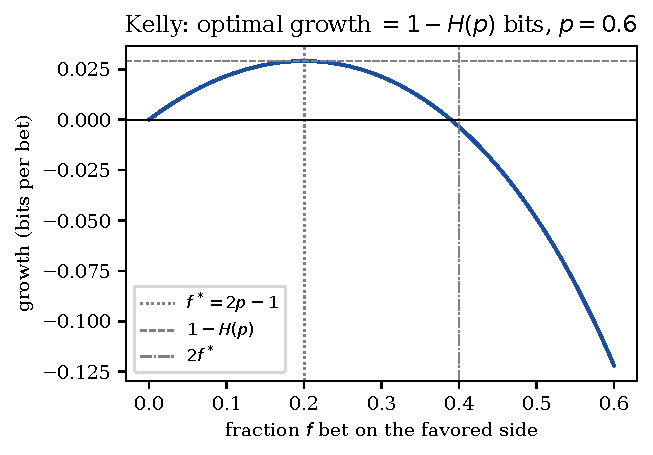
\includegraphics[width=0.92\textwidth]{kelly}
\caption{Kelly growth rate in bits per bet for $p=0.6$ at even odds. The maximum at $f^*=2p-1$ (dotted vertical line) equals $1-H(p)$ (dashed horizontal line). The curve crosses zero at $f\approx0.389$, just below $2f^*=0.4$ (dash dotted vertical line), where the growth is slightly negative.}
\label{fig:kelly}
\end{figure}

\section{Learning systems as thermodynamic engines}

A learning system observes data, updates an internal model, and acts. The data processing inequality states that for a Markov chain $\Theta\to Y\to Z$, $I(\Theta;Z)\leq I(\Theta;Y)$: no processing of the data can increase its information about the truth. Consider a model that is retrained repeatedly on its own outputs.

\begin{proposition}[Recursive self learning]\label{prop:recursive_self_learning}%
Let $\Theta$ be a target and let $M_0$ be a model with $I(\Theta;M_0) = i_0$. Suppose $M_{k+1}$ is computed from $M_k$ and from fresh randomness independent of $\Theta$. Then $I(\Theta;M_k)\leq i_0$ for all $k$. If at each round the update also uses the output of a verifier $V_k$ that depends on $\Theta$ through a channel of capacity $C$ bits per round, so that $I(\Theta;V_k\mid M_k)\leq C$, then $I(\Theta;M_k)\leq i_0+kC$.
\end{proposition}

\begin{proof}
In the first case $\Theta\to M_k\to M_{k+1}$ is a Markov chain and the data processing inequality applies. In the second, by the chain rule, $I(\Theta;M_{k+1})\leq I(\Theta;M_k,V_k)\leq I(\Theta;M_k)+I(\Theta;V_k\mid M_k)\leq I(\Theta;M_k)+C$.
\end{proof}

The proposition is simple, but it sets the terms of debates about systems that improve by self play or by training on synthetic data. AlphaZero~\cite{silver2018} is an analogy for the second clause rather than an instance of it. The rules of chess are a perfect verifier, every game ends in a win, draw or loss determined by the rules, and self play converts computation into play of superhuman strength. In the analogy the unknown $\Theta$ is the value of the positions, and each game returns a result that carries at most $\log_23$ bits about it. The analogy is imperfect, because the value of a position is a deterministic consequence of rules that the learner already has: what self play adds is computation on known rules, which is logical rather than statistical information, and the bound $i_0+kC$ does not describe it as stated. In our paper on AI assisted research~\cite{polsonsokolov2026air} we argue that mathematics has the same structure, since proofs can be checked, and that a research program in which a model proposes and a verifier, human or formal, checks behaves like a digital twin of self play. The present book, drafted with extensive machine assistance and reviewed by its authors, is a small instance.

Each round of learning that overwrites a model's parameters removes entropy from the memory that holds them, and by Theorem~\ref{thm:landauer} the minimum dissipation is $k_BT\log2$ times the entropy removed, measured in bits. Overwriting a value that is known in advance removes no entropy and costs nothing in principle. The information gained per round is at most $C$ bits. The thermodynamic efficiency of learning is therefore bounded by the ratio of verified bits gained to bits of entropy removed, and a learning system that removes far more entropy than it learns, as all present digital systems do, operates far from the Landauer limit. A power budget $P$ pays for the removal of at most $P/(k_BT\log2)$ bits of entropy per second, which for the brain's twenty watts is the ceiling discussed in Chapter~\ref{ch:filters}.

\section{Cybernetics revisited}

Wiener defined cybernetics as the science of control and communication in the animal and the machine. Its central notions, feedback, information and homeostasis, were mathematized in the two decades that followed: feedback by the control theory of Pontryagin and Kalman, information by Shannon and Kolmogorov, homeostasis by the stability theory of dynamical systems. What was missing was a theory of learning that was at once statistical, computational and physical. The chapters of Part~\ref{part:statmech} supply pieces of one. Hilbert asked for the axioms of physics; Kolmogorov's lecture can be read as a request for the physics of thought; the two requests meet in the theory of Bayesian inference as a physical process.

\section{Fluctuation theorems}

Landauer's bound (Theorem~\ref{thm:landauer}) is an inequality on average. Its refinements are equalities about fluctuations. Consider a system in equilibrium at inverse temperature $\beta = 1/k_BT$ with Hamiltonian $\mathcal H_{\lambda_0}$, driven by changing a control parameter from $\lambda_0$ to $\lambda_1$ over a finite time, and let $W$ be the work performed along a trajectory.

\begin{theorem}[Jarzynski]
Under Hamiltonian dynamics, or under any Markov dynamics that preserves the instantaneous Gibbs measure for each fixed value of the control,
\[
\E\big[e^{-\beta W}\big] = e^{-\beta\Delta F},\qquad\Delta F = -\beta^{-1}\log\frac{Z_{\lambda_1}}{Z_{\lambda_0}}.
\]
\end{theorem}

\begin{proof}[Proof for Hamiltonian dynamics]
For an isolated system the work is $W = \mathcal H_{\lambda_1}(\Phi(x))-\mathcal H_{\lambda_0}(x)$, where $\Phi$ is the volume preserving flow map. Then
\[
\begin{aligned}\E e^{-\beta W} &= \int\frac{e^{-\beta\mathcal H_{\lambda_0}(x)}}{Z_{\lambda_0}}e^{-\beta(\mathcal H_{\lambda_1}(\Phi(x))-\mathcal H_{\lambda_0}(x))}\dd x\\ &= \frac{1}{Z_{\lambda_0}}\int e^{-\beta\mathcal H_{\lambda_1}(\Phi(x))}\dd x = \frac{Z_{\lambda_1}}{Z_{\lambda_0}},\end{aligned}
\]
by Liouville's theorem.
\end{proof}

\begin{proof}[Proof for Markov dynamics in discrete time]
Let the control take the values $\mu_0 = \lambda_0,\mu_1,\dots,\mu_N = \lambda_1$ in turn. At step $k$ the control moves from $\mu_{k-1}$ to $\mu_k$ with the state $x_{k-1}$ held fixed, which costs the work $w_k(x_{k-1})$ with $w_k(x) = \mathcal H_{\mu_k}(x)-\mathcal H_{\mu_{k-1}}(x)$, and then the state moves to $x_k$ by a Markov kernel $K_{\mu_k}$ that leaves the Gibbs density $\pi_{\mu_k} = e^{-\beta\mathcal H_{\mu_k}}/Z_{\mu_k}$ invariant. The total work is $W = \sum_{k=1}^Nw_k(x_{k-1})$. Since $\pi_{\mu_{k-1}}(x)e^{-\beta w_k(x)} = (Z_{\mu_k}/Z_{\mu_{k-1}})\pi_{\mu_k}(x)$, integrating out $x_0,x_1,\dots$ in turn and using $\int\pi_{\mu_k}(x)K_{\mu_k}(x,y)\dd x = \pi_{\mu_k}(y)$ at each step gives $\E e^{-\beta W} = \prod_{k=1}^NZ_{\mu_k}/Z_{\mu_{k-1}} = Z_{\lambda_1}/Z_{\lambda_0}$.
\end{proof}

The equality is due to Jarzynski~\cite{jarzynski1997}. For Markov dynamics see Jarzynski~\cite{jarzynski1997master}, who works with a master equation, and Crooks~\cite{crooks2000}, who works in discrete time as above.

Jensen's inequality gives $\E W\geq\Delta F$, the second law, as a consequence. The equality is a change of measure identity: it is importance sampling, with the nonequilibrium trajectory as proposal and the target equilibrium as goal, and it is the physical form of the annealed importance sampling algorithm that Neal introduced independently in 2001~\cite{neal2001}, and of the sequential Monte Carlo samplers of Del Moral, Doucet and Jasra~\cite{delmoral2006}. Crooks' theorem~\cite{crooks1999}, which we quote without proof, refines it to a statement about the ratio of the work density $p_F(W)$ of the protocol to the work density $p_R(-W)$ of the time reversed protocol started in equilibrium at $\lambda_1$, $p_F(W)/p_R(-W) = e^{\beta(W-\Delta F)}$, which is a likelihood ratio between time reversed path measures.

Sagawa and Ueda~\cite{sagawaueda2010} extended the second law to systems with measurement and feedback, and we quote their inequality without proof. If a measurement yields mutual information $I$, in nats, between the system and the memory, and the protocol is chosen as a function of the outcome, then
\[
\E W\geq\Delta F-\beta^{-1}I,
\]
so that information can be converted into work at the rate $k_BT$ per nat, exactly Szilard's rate, and a corresponding cost must be paid when the memory is reset. The generalized second law is the thermodynamic counterpart of the data processing inequality: information is a resource, measured in the same units as free energy, and it can be spent but not created.

\section{Rate distortion and the cost of approximate inference}

Shannon's rate distortion theory asks for the minimal number of bits per symbol needed to describe a source $X$ to within expected distortion $D$:
\[
R(D) = \min_{p(\hat x\mid x):\,\E d(X,\hat X)\leq D}I(X;\hat X).
\]
For a Gaussian source with variance $\sigma^2$ and squared error distortion, $R(D) = \frac12\log_2(\sigma^2/D)$ for $D<\sigma^2$, as in Cover and Thomas~\cite{covertomas}. The minimizing channel is a Gaussian posterior: the optimal reconstruction is the posterior mean under a Gaussian prior and observation model. Rate distortion is therefore Bayesian inference read backwards.

Combined with Landauer's principle, rate distortion theory gives a thermodynamic floor for storing approximations. Let $X_1,\dots,X_n$ be independent copies of the source, and let a memory with finitely many states hold reconstructions $\hat X_1,\dots,\hat X_n$ with average distortion at most $D$. Then $H(\hat X_{1:n})\geq I(X_{1:n};\hat X_{1:n})\geq nR(D)$, which is the converse half of the rate distortion theorem, and by Theorem~\ref{thm:landauer} resetting the memory dissipates at least $nR(D)\,k_BT\log2$ on average. For inference, the source is the unknown quantity and the reconstruction is the stored estimate of it.

Blahut's algorithm~\cite{blahut1972} for computing $R(D)$, a counterpart of Arimoto's algorithm for the capacity of a channel~\cite{arimoto1972}, is an alternating minimization of relative entropy of the same type as Sinkhorn's algorithm of Chapter~\ref{ch:gbc}, with the distortion playing the role of the transport cost and the Lagrange multiplier the role of the inverse entropic regularization. It fixes only the marginal of the source, whereas Sinkhorn's algorithm fixes both marginals.

\section*{Exercises}
\begin{enumerate}
\item Compute the Kelly fraction and the optimal growth rate for a bet that returns $o$ on a unit stake if it is won, the convention of Theorem~\ref{thm:kelly}, with win probability $p$ and $po>1$. Even odds are $o = 2$.
\item Show that betting $2f^*$ in the even odds Kelly problem gives growth $-\frac{4}{3\ln2}(2p-1)^4+O\big((2p-1)^6\big)$ bits per bet, which is negative, whereas the growth at $f^*$ is of order $(2p-1)^2$.
\item Prove the data processing inequality from the chain rule for mutual information.
\item Deduce $\E W\geq\Delta F$ from Jarzynski's equality, and show that $\P(W\leq\Delta F-\varepsilon)\leq e^{-\beta\varepsilon}$.
\item Compute $R(D)$ for a Bernoulli$(p)$ source with Hamming distortion.
\end{enumerate}


\section*{Notes}

Our paper with Alec Litowitz~\cite{litowitz2026} follows the line from Shannon's theory of communication to Kolmogorov's theory of complexity. Leff and Rex's anthology \emph{Maxwell's Demon}~\cite{leffrex1990} collects the classical papers of Szilard, Landauer and Bennett. Cover and Thomas~\cite{covertomas} treat Kelly gambling and the data processing inequality. Li and Vit\'anyi's monograph~\cite{livitanyi2008} is the standard reference for Kolmogorov complexity.

\chapter{Open Problems and the Bridge to Hilbert's Eighth Problem}
\label{ch:open}

\section{Two problems about the heat equation}

Hilbert's eighth problem contains the Riemann hypothesis. It appears in a list about prime numbers, far from the axioms of physics, and the two problems are usually treated as belonging to different worlds. This chapter points to a common mathematical structure. The Riemann hypothesis is equivalent to a statement about the backward flow of the heat equation, and the inferential form of the sixth problem, which asks to recover the initial state of a dissipative system from later observations, is a backward problem for a parabolic equation. This is an analogy and not an equivalence. Both have probabilistic formulations in terms of Brownian motion, and the eighth problem has a natural expression in the language of ferromagnetic random variables that Lee, Yang and Newman developed for statistical mechanics.

\section{The de Bruijn Newman constant}

Let $\xi(s) = \frac12s(s-1)\pi^{-s/2}\Gamma(s/2)\zeta(s)$ and $\Xi(x) = \xi(\frac12+ix)$. Riemann's representation of $\Xi$ as a Fourier transform~\cite{riemann1859}, which P\'olya wrote with an explicit kernel~\cite{polya1926}, reads in the scaling of Rodgers and Tao~\cite{rodgerstao2020}
\begin{gather*}
\Xi(x) = 8\int_0^\infty\Phi(u)\cos(2xu)\dd u, \\
\Phi(u) = \sum_{n=1}^\infty\big(2\pi^2n^4e^{9u}-3\pi n^2e^{5u}\big)\exp\big(-\pi n^2e^{4u}\big),
\end{gather*}
where $\Phi$ is even in $u$ when extended to the line, positive, rapidly decreasing, and decreasing on $(0,\infty)$. The Riemann hypothesis is the statement that all zeros of $\Xi$ are real. Following de Bruijn~\cite{debruijn1950} and Newman~\cite{newman1976}, define for $t\in\R$
\[
H_t(z) = \int_0^\infty e^{tu^2}\Phi(u)\cos(zu)\dd u,
\]
so that $H_0(z) = \frac18\Xi(z/2)$, whose zeros are at $\pm2\gamma_n$ where $\frac12+i\gamma_n$ are the nontrivial zeros of $\zeta$. Differentiating under the integral,
\[
\partial_tH_t(z) = \int_0^\infty u^2e^{tu^2}\Phi(u)\cos(zu)\dd u = -\partial_z^2H_t(z).
\]
Thus $H_t$ solves the backward heat equation in $z$: increasing $t$ runs the heat flow backwards.

Riemann's memoir of 1859, \emph{\"Uber die Anzahl der Primzahlen unter einer gegebenen Gr\"osse}~\cite{riemann1859}, introduced the zeta function as a function of a complex variable, proved its functional equation, wrote the function now denoted $\Xi$ as a cosine transform, and stated that it is very probable that all of its roots are real. Riemann's sentence is a statement about a Fourier transform. P\'olya pursued this reading in the 1920s. In 1926 P\'olya observed that the leading term of $\Phi$ at infinity, used on one side only, gives a Fourier transform with infinitely many nonreal zeros, whereas an even kernel with the same behavior at both ends of the line gives one with only real zeros~\cite{polya1926}. In 1927 P\'olya studied trigonometric integrals with only real zeros more generally~\cite{polya1927}. De Bruijn introduced the Gaussian factors $e^{\lambda u^2}$ in 1950~\cite{debruijn1950}, and Newman turned this family into the definition of $\Lambda$~\cite{newman1976}.

\begin{definition}[Laguerre P\'olya class]\label{def:laguerrepolya}
An entire function belongs to the Laguerre P\'olya class if it is a locally uniform limit of real polynomials with only real zeros. Equivalently, by the theorem of Laguerre and P\'olya~\cite[Chapter~VIII]{levin1964}, it has the form
\[
F(z) = cz^me^{-az^2+bz}\prod_k\Big(1-\frac{z}{z_k}\Big)e^{z/z_k},
\]
with $m$ a nonnegative integer, $a\geq0$, $b,c$ and $z_k\neq0$ real, and $\sum z_k^{-2}<\infty$.
\end{definition}

\begin{theorem}[P\'olya~\cite{polya1927}, de Bruijn~\cite{debruijn1950}]\label{thm:polyadebruijn}
Let $F$ be an even real entire function of order less than $2$, not identically zero, with only real zeros, and let $\lambda\geq0$. Then the series $e^{-\lambda D^2}F = \sum_{j\geq0}\frac{(-\lambda)^j}{j!}F^{(2j)}$, where $D = \frac{\dd}{\dd z}$, converges locally uniformly, and $e^{-\lambda D^2}F$ is an even function in the Laguerre P\'olya class. In particular, if $H_t$ has only real zeros for some $t$, then $H_{t'}$ has only real zeros for every $t'\geq t$.
\end{theorem}

\begin{proof}
Let $p$ be a real polynomial of degree $d\geq1$ with only real zeros and let $s>0$. Then $(1+sD)p = se^{-x/s}\frac{\dd}{\dd x}\big(e^{x/s}p\big)$ has degree $d$. The function $e^{x/s}p$ tends to $0$ as $x\to-\infty$ and vanishes at the zeros of $p$, so by Rolle's theorem its derivative vanishes to the left of the smallest zero and between any two distinct zeros, and at a zero of multiplicity $k$ it vanishes to order $k-1$. These real zeros number $d$, so $(1+sD)p$ has only real zeros, and the same argument with $e^{-x/s}p$ and $+\infty$ applies to $(1-sD)p$. Since $1-s^2D^2 = (1-sD)(1+sD)$, the polynomial $(1-\frac\lambda nD^2)^np$ has only real zeros for every $n$, and it converges coefficientwise to $e^{-\lambda D^2}p$ as $n\to\infty$. Zeros depend continuously on the coefficients, so $e^{-\lambda D^2}p$ has only real zeros.

Now let $F$ be as in the theorem. By Hadamard's theorem $F(z) = Cz^{2m}\prod_{k\geq1}(1-z^2/z_k^2)$ with $z_k>0$ and $\sum_kz_k^{-2\alpha}<\infty$ for some $\alpha\in(0,1)$. The partial products $F_n$ are real polynomials with only real zeros that converge to $F$ locally uniformly, and since $\log(1+x)\leq x^\alpha/\alpha$ for $x\geq0$, $|F_n(z)|\leq A(1+|z|)^{2m}e^{S|z|^{2\alpha}}$ with $A$ and $S$ independent of $n$. Cauchy's estimate on the circle of radius $2\sqrt{\lambda j}$ about $z$, together with $(2j)!/j!\leq(2j)^j$, bounds the $j$th term $\frac{\lambda^j}{j!}|F_n^{(2j)}(z)|$ by $2^{-j}$ times the maximum of $|F_n|$ on that circle, and this maximum is $\exp(O(j^\alpha))$ with $\alpha<1$, uniformly in $n$ and locally uniformly in $z$. Hence the series for $e^{-\lambda D^2}F$ and for $e^{-\lambda D^2}F_n$ converge locally uniformly, and $e^{-\lambda D^2}F_n\to e^{-\lambda D^2}F$. The polynomials $e^{-\lambda D^2}F_n$ are real with only real zeros, so the limit belongs to the Laguerre P\'olya class, and it is even because $D^2$ preserves parity.

Finally, differentiating under the integral sign gives $H_t^{(2j)}(z) = (-1)^j\int_0^\infty u^{2j}e^{tu^2}\Phi(u)\cos(zu)\dd u$, and summing over $j$ with Fubini's theorem gives $e^{-\lambda D^2}H_t = H_{t+\lambda}$. The kernel $e^{tu^2}\Phi(u)$ decays like $\exp(-\pi e^{4u}+O(u^2))$, so $H_t$ is an even real entire function of order at most $1$, and $H_t(0)>0$. If $H_t$ has only real zeros, the first part applies to $F = H_t$, so $H_{t'} = e^{-(t'-t)D^2}H_t$ is a locally uniform limit of real polynomials with only real zeros. It is not identically zero, so by Hurwitz's theorem it has only real zeros.
\end{proof}

The operator $e^{-\lambda D^2}$ is the backward heat semigroup, and the theorem says that it preserves the reality of the zeros of even functions of order less than $2$. By Hurwitz's theorem the set of $t$ for which $H_t$ has only real zeros is also closed, because $H_t\to H_{t_0}$ locally uniformly as $t\to t_0$. The set is therefore a half line as soon as it is known to be nonempty, which is due to de Bruijn, and not the whole line, which is due to Newman.

\begin{theorem}[de Bruijn Newman constant]\label{thm:lambda}
There is a constant $\Lambda\in\R$ such that $H_t$ has only real zeros if and only if $t\geq\Lambda$. De Bruijn proved $\Lambda\leq\frac12$ in 1950~\cite{debruijn1950}. Newman proved $\Lambda>-\infty$ in 1976 and conjectured $\Lambda\geq0$~\cite{newman1976}. Rodgers and Tao proved $\Lambda\geq0$ in a paper posted in 2018 and published in 2020~\cite{rodgerstao2020}. Polymath proved $\Lambda\leq0.22$ in 2019~\cite{polymath2019}, and Platt and Trudgian improved this to $\Lambda\leq0.2$ in a paper posted in 2020 and published in 2021~\cite{platttrudgian2021}. The Riemann hypothesis is equivalent to $\Lambda\leq0$, hence to $\Lambda = 0$.
\end{theorem}

We quote the bounds in this theorem without proof. The existence of $\Lambda$ follows from the bounds of de Bruijn and Newman, Theorem~\ref{thm:polyadebruijn} and Hurwitz's theorem, as explained before the statement, and the equivalence with the Riemann hypothesis follows from $H_0(z) = \frac18\Xi(z/2)$. Newman described the conjecture, now a theorem, as the statement that if the Riemann hypothesis is true, it is only barely so: running the heat flow forward by any amount from $t = 0$, which smooths the function in $z$, destroys the reality of the zeros. Figure~\ref{fig:debruijn_newman} shows the P\'olya kernel and the normalized functions $H_t$ for $t = -4,0,4$. The first three zeros of $H_0$, computed from the kernel by quadrature, lie at $28.27$, $42.04$ and $50.02$, twice the ordinates $14.13$, $21.02$ and $25.01$ of the first zeta zeros. As $t$ increases they move toward the origin, to $25.99$, $39.14$ and $47.64$ at $t = 4$, and as $t$ decreases they spread out, to $30.62$, $45.20$ and $52.29$ at $t = -4$.

\begin{figure}[t]
\centering
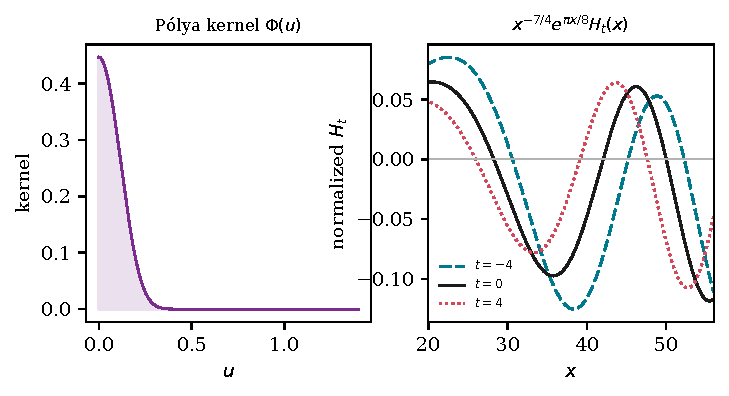
\includegraphics[width=\textwidth]{debruijn_newman}
\caption{Left, the P\'olya kernel $\Phi$. Right, $x^{-7/4}e^{\pi x/8}H_t(x)$ for $20\leq x\leq56$, computed by quadrature, for $t=-4$, $t=0$ (solid) and $t=4$, as marked in the legend. The factor $x^{-7/4}e^{\pi x/8}$ cancels the envelope $x^{7/4}e^{-\pi x/8}$ of $H_0$, which comes from the Gamma factor in $\xi$. The zeros of $H_0$ are twice the ordinates of the zeta zeros.}
\label{fig:debruijn_newman}
\end{figure}

The motion of the zeros has a formal description. If $H_t$ were a polynomial with simple zeros $z_k(t)$, differentiating $H_t(z_k(t)) = 0$ in $t$ and using the heat equation would give
\[
\dot z_k = \frac{\partial_z^2H_t(z_k)}{\partial_zH_t(z_k)} = 2\sum_{j\neq k}\frac{1}{z_k-z_j},
\]
a system of particles with logarithmic interaction, the same structure as Dyson's Brownian motion of Chapter~\ref{ch:brownian} without the noise. For entire functions of order one the sum must be interpreted with care, and Csordas, Smith and Varga~\cite{csv1994} made the description rigorous in a form sufficient to show that real zeros cannot collide and leave the real line under the backward flow. The proof of $\Lambda\geq0$ by Rodgers and Tao analyzes this dynamics, showing that if $\Lambda<0$ the zeros at $t = 0$ would be too regularly spaced, in contradiction with what is known about pair correlations of zeta zeros.

The analogy with Chapter~\ref{ch:nsinference} is formal. There, information about the initial condition of a dissipative equation is destroyed by forward evolution and must be recovered by backward inference, which is unstable at high frequencies. Here, the question is whether a structural property of an entire function, reality of zeros, survives backward evolution. The common structure is a Gaussian factor in Fourier space, $e^{-\nu|k|^2t}$ there and $e^{tu^2}$ here, and the analogy goes no further: the unknown there is an initial condition recovered from noisy data, and the function here is fixed.

\section{The Riemann hypothesis as a Lee Yang property}\label{sec:leeyangrh}

Let $X$ be a random variable with the symmetric density $\Phi(|u|)/\int_\R\Phi(|v|)\dd v$, which we call the P\'olya law. Its characteristic function is $\Xi(x/2)/\Xi(0)$, and its moment generating function is
\[
\E e^{sX} = \frac{\Xi(-is/2)}{\Xi(0)}.
\]
\begin{proposition}\label{prop:polyaleeyang}
The Riemann hypothesis holds if and only if the P\'olya law has the Lee Yang property of Chapter~\ref{ch:mixtures}.
\end{proposition}

\begin{proof}
The function $s\mapsto\E e^{sX} = \Xi(-is/2)/\Xi(0)$ is entire, because $\Phi(u)$ decays like $\exp(-\pi e^{4|u|})$ so that all exponential moments exist. Its zeros are the points $s$ with $\Xi(-is/2) = 0$, that is $s = 2ix$ with $\Xi(x) = 0$. Hence the zeros of the moment generating function are purely imaginary if and only if all zeros of $\Xi$ are real, which is the Riemann hypothesis since $\Xi(x) = \xi(\frac12+ix)$.
\end{proof} This is Newman's reformulation of 1976~\cite{newman1976}. In it, $e^{tu^2}$ is a Gaussian tilt of the single spin measure, and the de Bruijn Newman constant is the smallest $t$ for which the tilted P\'olya law has the Lee Yang property. Newman's motivation was a characterization of measures $\rho$ for which all ferromagnetic systems of spins with single spin law $\rho$ satisfy the Lee Yang theorem, and the Riemann hypothesis asks whether the P\'olya law belongs to a closely related class.

This reformulation explains why statistical mechanics enters number theory. Newman's theorem says that ferromagnetic couplings preserve the Lee Yang property. Multiplying a law with the Lee Yang property by $e^{bx^2}$ with $b\geq0$ preserves the property (Section~\ref{sec:ferromagnetic}, where it is derived from Newman's theorem by coupling to independent Ising spins). The Hubbard Stratonovich transformation writes this tilt as integrating out a Gaussian spin. It shows that if the tilted P\'olya law has the Lee Yang property at $t$, then it has the property at every larger $t$, which is Theorem~\ref{thm:polyadebruijn} again in the language of Chapter~\ref{ch:mixtures}. A proof of the Riemann hypothesis along these lines would exhibit the P\'olya law, which is the tilted law at $t = 0$, as a limit of ferromagnetic constructions. The companion volume~\cite{polsonh8} pursues a related route through Thorin measures: whether the reciprocal of $\Xi$, suitably normalized, is the Laplace transform of a generalized Gamma convolution, a positivity statement that is equivalent to the Riemann hypothesis.

\section{A Bayesian reading of the de Bruijn flow}

The family $e^{tu^2}\Phi(u)$, normalized, is an exponential family in the natural parameter $t$ with sufficient statistic $u^2$. Its characteristic functions are $H_t$, up to normalization. In the language of Chapter~\ref{ch:types}, varying $t$ is exponential tilting. The conditional limit theorem, which holds beyond finite alphabets under integrability conditions~\cite{csiszar1984}, identifies the tilted law as the limiting conditional law of one coordinate of a large P\'olya sample given its empirical second moment, and the integrability condition holds for every $t$ because $e^{tu^2}\Phi(u)$ is integrable. The de Bruijn flow is therefore the flow of conditional laws of a P\'olya distributed sample as the conditioning value of the empirical second moment increases. The Riemann hypothesis is the statement that the Lee Yang property holds at $t = 0$, which is conditioning on the typical value of the empirical second moment and returns the P\'olya law itself, and the theorem $\Lambda\geq0$ says that the property fails for every $t<0$, that is, for every conditioning value below the typical one. This reading suggests studying the constant through concentration and large deviation bounds for samples conditioned on their second moment.

\section{The Riemann hypothesis as a statement about Brownian motion}

Theorem~\ref{thm:bpy} of Biane, Pitman and Yor expresses $2\xi(s)$ as the Mellin transform $\E Y^s$ of a rescaled maximum of a Brownian excursion. The zeros of $\xi$ are the complex values of $s$ at which this Mellin transform vanishes. The Riemann hypothesis is therefore a statement about the law of a functional of Brownian motion: its Mellin transform vanishes only on the critical line. Several equivalent laws arise in the same paper, including the range of a Brownian bridge and sums of independent hitting times of Bessel processes, and the latter are generalized Gamma convolutions whose Thorin measures are explicit. The Brownian representation and the Thorin representation are two faces of the same object, and the passage between them is Kent's spectral theorem of Chapter~\ref{ch:brownian}.

\section{A computational strategy}

The Thorin measure of a GGC can be estimated from its Laplace transform by inverting the Stieltjes transform of the derivative of the Laplace exponent. For the reciprocal $\Xi$ problem, the Riemann hypothesis predicts a specific discrete Thorin measure supported on the squares of the zero ordinates. One can estimate the Thorin measure numerically from high precision evaluations of $\Xi$ and compare it with the measure predicted by the hypothesis, as a function of the truncation level. The predicted measure is purely atomic, and an estimate computed at a finite truncation level has a density or has its atoms elsewhere, so the two measures are mutually singular and their total variation distance would not tend to zero. The comparison must use a weak metric, such as the Wasserstein or L\'evy Prokhorov distance on windows, or compare Stieltjes transforms. Agreement to numerical precision on any finite window is not a proof, but the comparison isolates which positivity property would need to be proved, and it is the same kind of numerical certificate that the Yor identities of Chapter~\ref{ch:brownian} provide for their algorithms.

\section{Open problems}

We close with open problems drawn from the chapters of the book. Some are precise questions and some are programs, which we mark as such.

\begin{problem}[The inferential sixth problem]
This is a program, and its first task is to fix the regime. Consider hard spheres in the Boltzmann Grad limit with Gibbs initial data conditioned on a macroscopic density, velocity and temperature profile, observed through the hydrodynamic fields at a later time with noise of standard deviation $\sigma$. Find a relation between $\sigma$, the Knudsen number and the number of particles under which the deviation of the particle fields from the solution of the limiting fluid equations is small compared with $\sigma$, and prove under it a Bernstein von Mises theorem for smooth functionals of the initial macroscopic profile, with constants that do not depend on the number of particles.
\end{problem}

\begin{problem}[Poincar\'e]
Give quantitative versions of the method of arbitrary functions (Theorem~\ref{thm:arbitrary}) for mixed phase space systems such as H\'enon Heiles, where invariant tori and chaotic regions coexist, with rates in terms of the measure of the chaotic sea.
\end{problem}

\begin{problem}[Axioms]
Quantitative estimates for chaos and entropic chaos in Kac's model are known in several forms. Carlen, Carvalho, Le Roux, Loss and Villani~\cite{cclv2010} relate propagation of chaos to entropy and show, in particular, that the entropic rate of convergence to equilibrium can be arbitrarily slow. Hauray and Mischler~\cite{hauraymischler2014} compare Kac's chaos, entropic chaos and Fisher information chaos quantitatively, extend the estimates to measures on the Kac spheres, and treat mixtures in the sense of de Finetti, Hewitt and Savage. We do not know whether these estimates are optimal. Find the optimal rate, as a function of the marginal size $k$ and of $N$, in the finite de Finetti theorem for exchangeable laws on the sphere $S^{N-1}(\sqrt N)$ in relative entropy, with examples showing that it cannot be improved, and use it to prove a propagation of chaos theorem for Kac's model whose dependence on $N$ is optimal under explicit hypotheses on the initial law.
\end{problem}

\begin{problem}[Yor identities]
\label{prob:yor}
This is a program. Kent's theorem~\cite{kent1980} writes the hitting time of a level by a regular diffusion, started at a reflecting or entrance boundary, as a sum $\sum_nE_n/\lambda_n$ of independent exponential variables, where the $\lambda_n$ are eigenvalues of the generator. The part of the sum after the first $n$ terms is a generalized Gamma convolution with an explicit Thorin measure. Identify a class of regular diffusions for which this remainder can be sampled exactly with finite expected cost, prove that the resulting sampler is exact, and use it to build a library of exact samplers for Brownian functionals.
\end{problem}

\begin{problem}[Mixtures]
By Khintchine's theorem the P\'olya law of Section~\ref{sec:leeyangrh} is the law of $UZ$ with $U$ uniform on $[-1,1]$ and $Z\geq0$ independent of $U$. The law of $Z$ is not a generalized Gamma convolution, because $Z$ has finite exponential moments of every order and a nonconstant generalized Gamma convolution does not. The reciprocal of the moment generating function of $UZ$ at $2\sqrt\lambda$ is a different matter. It is $\Xi(0)/\Xi(i\sqrt\lambda) = \prod_n(1+\lambda/\gamma_n^2)^{-1}$, where $\pm\gamma_n$ are the zeros of $\Xi$, and it is the Laplace transform of a generalized Gamma convolution if and only if the Riemann hypothesis holds. In that case the Thorin measure is the sum of point masses at the $\gamma_n^2$. Conversely, the logarithmic derivative of the Laplace transform of a generalized Gamma convolution is analytic outside the negative half line, which forces all the $\gamma_n^2$ to be positive. Prove that this function is the Laplace transform of a generalized Gamma convolution by using the mixture representation $X = UZ$ and not the location of the zeros.
\end{problem}

\begin{problem}[Perelman]
Ni~\cite{ni2004} proved that the analog of the entropy $W$ of Theorem~\ref{thm:perelman_flat} for the linear heat equation on a Riemannian manifold is nonincreasing when the Ricci curvature is nonnegative. Extend the scale mixture proof of the monotonicity of $W$ (Theorem~\ref{thm:perelman_flat}) to Riemannian manifolds with nonnegative Ricci curvature, interpreting the Ricci term as a correction to the subordinated Brownian motion.
\end{problem}

\begin{problem}[Quantum]
Formulate a prior on Nelson's diffusions that does not itself impose the quantization condition, and identify data that determine the circulation of the drift around the nodes of the density, so that the posterior concentrates on drifts satisfying the quantization condition. Position statistics alone fix the density and, through the continuity equation, only the divergence of the current, so the data must carry more. A solution would give a Bayesian answer to Wallstrom's objection.
\end{problem}

\begin{problem}[Kinetic]
\label{prob:kinetic}
For the $N$ particle Kac walk with total collision rate $N$, let $H_N(F) = \int F\log F\dd\sigma_N$ be the relative entropy of a probability density $F$ with respect to the uniform law $\sigma_N$ on $S^{N-1}(\sqrt N)$, and let $D_N(F)$ be the rate at which $H_N$ decreases at time zero along the master equation started at $F$. Villani's argument~\cite{villani2003cercignani} gives $D_N(F)\geq2H_N(F)/(N-1)$. The best constant in this inequality tends to zero with $N$~\cite{cclv2010} and is at most $C_bN^{-1+2b}\log N$ for every $0<b<\frac16$, with $C_b$ depending only on $b$~\cite{einav2011}; Gao, Wang and Xia~\cite{gaowangxia2026} prove in a recent preprint that it equals $2/(N-1)$ for every $N\geq2$. The near extremal densities in these three works are conditioned products $F^f_N(v) = Z_N(f)^{-1}\prod_{i\leq N}f(v_i)$, where $f$ is a probability density on $\R$ and $Z_N(f) = \int\prod_{i\leq N}f(v_i)\,\sigma_N(\dd v)$. In the first two, $f$ is a mixture of two centered Gaussian densities, normalized to unit variance, with a fourth moment that is unbounded along the construction. Gao, Wang and Xia use two families: mixtures of two centered Gaussian densities, whose mixing law has two atoms and so is not a generalized Gamma convolution, and $f$ proportional to $(a+v^2)^{-q}$, with $a\to0$ and then $q\to\frac12$ at fixed $N$. The latter $f$ is a rescaled Student law with $2q-1$ degrees of freedom, hence a normal scale mixture whose inverse Gamma mixing law is a generalized Gamma convolution (Appendix~\ref{app:levy}); its variance tends to zero or is infinite, and the energy concentrates on one particle. Without moment conditions, restricting $f$ to such mixtures therefore does not improve the constant $2/(N-1)$. Fix $M>3$, and let $\mathcal G_M$ be the set of bounded densities $f$ that are normal scale mixtures with generalized Gamma convolution mixing law and satisfy $\int v^2f(v)\dd v = 1$ and $\int v^4f(v)\dd v\leq M$. Decide whether there is $\lambda>0$, depending only on $M$, such that $D_N(F^f_N)\geq\lambda H_N(F^f_N)$ for every $N\geq2$ and every $f\in\mathcal G_M$. Carlen, Carvalho, Le Roux, Loss and Villani~\cite{cclv2010} raise the question whether a fixed bound on the fourth moment gives a bound of this kind without the condition on the mixing law, and Carlen, Carvalho and Einav~\cite{carlencarvalhoeinav2018} prove inequalities of the weaker form $D_N(F)/N\geq C(H_N(F)/N)^{1+\varepsilon}$, with $C$ independent of $N$, for data with bounded moments that satisfy a quantitative form of chaos.
\end{problem}

\begin{problem}[Hydrodynamics]
Derive the incompressible Navier Stokes Fourier system from hard sphere dynamics in a bounded domain with Maxwell reflection boundary conditions, identifying the boundary layers in the limit. The torus in dimensions two and three is treated in the preprint~\cite{denghanima2025}, and the problem is the extension to domains with boundary.
\end{problem}

\begin{problem}[Inference]
\label{prob:inference}
Konen and Nickl~\cite{konennickl2026} prove a functional Bernstein von Mises theorem for the posterior of the trajectory of the two dimensional Navier Stokes equations on the torus, with root $N$ consistent prediction of future states in the supremum norm, for a Gaussian prior on the initial condition and $N$ noisy observations at uniformly random points of space and time. We know of no corresponding result for sensors at fixed locations or for other priors. Determine the posterior contraction rate for the initial vorticity from noisy point observations at a fixed array of sensors and times, in terms of the number of sensors, the number of times and the noise level, and identify the functionals of the initial vorticity that admit a Bernstein von Mises theorem. A companion question is whether the posterior of the initial vorticity can be computed in time polynomial in the data size and the dimension; Section~\ref{sec:gradstab} records what is known.
\end{problem}

\begin{problem}[Blowup]
Fix a finite horizon and a computable blowup criterion, for example that a norm of the solution of a Galerkin truncation of the equations exceeds a threshold before the horizon. Construct a prior on initial data and forcing for three dimensional Navier Stokes and a sequence of numerical solvers such that the posterior probability of this event is consistent, that is, converges to its true value as the resolution and the amount of data increase, and quantify how the event approximates finite time blowup of the exact solution. Consistency for the blowup of the exact solution itself, under either hypothesis, would require deciding the regularity of the data near the truth, which is the regularity problem.
\end{problem}

\begin{problem}[Onsager]
This is a program. At finite Reynolds number the velocity field is smooth, so a H\"older exponent has to be defined through an inertial range statement, such as the scaling $S_p(\ell)\propto\ell^{\zeta_p}$ of the structure functions. Develop a joint posterior for the exponents $\zeta_p$ and the inertial range from measured velocity increments, and use it to ask whether laboratory and numerical data concentrate at, above or below the exponents $\zeta_p = p/3$ of Kolmogorov and Onsager.
\end{problem}

\begin{problem}[Phase transitions]
Chapter~\ref{ch:spins} records what is known for the planted clique problem with a known clique size $k$ in the graph $G(n,\frac12)$: approximate message passing succeeds for $k\geq(1+\varepsilon)\sqrt{n/e}$, and from a suitable starting state the Metropolis process cannot find a planted clique of size $k = n^{1/2-\varepsilon}$ in polynomial time. Take as samplers of the posterior over clique locations either Glauber dynamics on vertex sets of size $k$, or Langevin dynamics for a continuous relaxation of the clique indicator, in both cases initialized from the prior. Determine whether such samplers have a computational phase transition at $k = \sqrt{n/e}$, in the sense that they succeed in polynomial time above $(1+\varepsilon)\sqrt{n/e}$ and fail below $(1-\varepsilon)\sqrt{n/e}$.
\end{problem}

\begin{problem}[Transport]
Prove convergence rates for generative Bayesian computation via learned Schr\"odinger bridges in terms of the entropic regularization, the number of simulations and the smoothness of the posterior. Rates in the sample size are known for the entropic optimal transport cost estimated from samples, by Genevay, Chizat, Bach, Cuturi and Peyr\'e~\cite{genevay2019} and by Mena and Niles Weed~\cite{menaniles2019}. The problem concerns the learned bridge as an estimator of the posterior.
\end{problem}

\begin{problem}[Thermodynamics of inference]
The Landauer bound (Theorem~\ref{thm:landauer}) bounds the heat dissipated by a physical process in terms of the entropy removed, and the Sagawa Ueda inequality of Chapter~\ref{ch:kolmogorov} bounds the work in terms of the mutual information acquired. For a Bayesian update from a prior $\mu_0$ to the posterior $\mu_y$, prove a lower bound on the heat dissipated by any physical implementation in terms of $\KL(\mu_y\|\mu_0)$ and the information erased, and compare it with the dissipation of Langevin samplers.
\end{problem}

\begin{problem}[The bridge]
This is a program whose goal is the Riemann hypothesis, which is equivalent to $\Lambda\leq0$. Newman's theorem (Chapter~\ref{ch:mixtures}) produces laws with the Lee Yang property from independent single spin laws with that property by ferromagnetic couplings. Decide whether the P\'olya law is the weak limit of a sequence of laws of random variables $X_n$ obtained by such constructions from Ising spins and uniform laws, with $\sup_n\E e^{c|X_n|}<\infty$ for every $c>0$, which is the control that carries the Lee Yang property to the limit by Hurwitz's theorem. A construction would prove the Riemann hypothesis by Proposition~\ref{prop:polyaleeyang}, and a proof that none exists would show that this route to the hypothesis is closed.
\end{problem}

\section{Conclusion}

Hilbert asked for the passage from atoms to continua with full rigor. A century and a quarter later the passage has been announced for a rarefied gas of hard spheres on the torus by Deng, Hani and Ma in two preprints~\cite{denghanima2024,denghanima2025}, building on the work of Lanford, Bardos, Golse, Levermore and Saint Raymond. Kolmogorov supplied the probability, Poincar\'e the warnings and the first rigorous mechanism of chance, Boltzmann the vision. The inverse passage, from continua back to the states that produced them, is younger and less complete. It rests on the same mathematics and it inherits the same limitations at the boundary of regularity. We have argued that Bayesian computation is the natural language for that inverse passage and that inference is itself a problem of statistical mechanics. If the argument is right, Hilbert's sixth problem is not closed; it has acquired a second half.

We do not claim a proof of the Riemann hypothesis, of the global regularity of the Navier Stokes equations, or of any of the open problems above. What we claim is structural. The mathematics that Hilbert's sixth problem required, probability measures on spaces of trajectories, entropy, transport and the heat equation, is also the mathematics in which the eighth problem has its probabilistic formulations, and the mathematics in which Bayesian computation is carried out. Several of the open problems, among them the last, ask for theorems about the heat equation, its backward flow and the measures it transports. The sixth problem taught that such theorems are about limits and about the measures on initial conditions with respect to which the limits hold. The inferential reading taught that those measures can be learned. Whether the same lessons apply to the zeros of $\Xi$ is, for now, an open question.

\section*{Exercises}
\begin{enumerate}
\item Justify differentiation under the integral sign in $\partial_tH_t = -\partial_z^2H_t$.
\item Show that $H_0(z) = \frac18\Xi(z/2)$.
\item For a real polynomial with simple real zeros evolving by $\partial_tp = -p''$, derive $\dot z_k = 2\sum_{j\neq k}(z_k-z_j)^{-1}$.
\item Show that $e^{-\lambda D^2}(z^2-1) = z^2-1-2\lambda$, and determine the values of $\lambda$, positive or negative, for which the zeros are real.
\item Express $\E Y^2$ and $\E Y^4$ in the Biane, Pitman and Yor identity through values of $\xi$, and evaluate them numerically.
\end{enumerate}


\section*{Notes}

De Bruijn~\cite{debruijn1950} proved a zero free strip bound, Theorem~13 of that paper: if $H_{t_0}$ has no zeros with $|\Im z|>y_0$, then for $t>t_0$ the function $H_t$ has none with $|\Im z|>\sqrt{\max(y_0^2-2(t-t_0),0)}$. The zeros of $H_0$ satisfy $|\Im z|<1$, so $t_0 = 0$ and $y_0 = 1$ give $\Lambda\leq\frac12$. The monotonicity in $t$ follows from results of P\'olya~\cite{polya1927}. Platt and Trudgian~\cite{platttrudgian2021} obtain $\Lambda\leq0.2$ by combining a conditional bound of the Polymath paper~\cite{polymath2019}, its Table~1, with their verification of the Riemann hypothesis up to height $3\cdot10^{12}$.


\appendix
\chapter{L\'evy Processes, Thorin Measures and Related Classes}
\label{app:levy}

This appendix collects the definitions and standard results on infinite divisibility used in the book. Proofs can be found in Sato~\cite{sato1999}, in Schilling, Song and Vondra\v{c}ek~\cite{schilling2012}, and in Bondesson~\cite{bondesson1992}; we give chapter or section numbers for the main facts.

\section{L\'evy processes}

A L\'evy process is a process $(X_t)_{t\geq0}$ with $X_0 = 0$, independent and stationary increments, and paths that are right continuous with left limits. Its law is determined by the law of $X_1$, which is infinitely divisible, and $\E e^{iuX_t} = e^{t\psi(u)}$ with $\psi$ given by the L\'evy Khintchine formula of Chapter~\ref{ch:mixtures}~\cite[Section~8]{sato1999}. The L\'evy It\^o decomposition~\cite[Chapter 4]{sato1999} writes $X$ as the sum of a drift, a Brownian motion and an independent pure jump process whose jumps form a Poisson point process with intensity $\dd t\otimes\nu(\dd x)$.

\section{Bernstein, Stieltjes and complete Bernstein functions}

A function $\phi:(0,\infty)\to[0,\infty)$ is a Bernstein function if it is smooth and $(-1)^{n-1}\phi^{(n)}\geq0$ for $n\geq1$. Equivalently $\phi(\lambda) = c+a\lambda+\int_0^\infty(1-e^{-\lambda x})\nu(\dd x)$ with $c,a\geq0$ and $\int(1\wedge x)\nu(\dd x)<\infty$~\cite[Chapter 3]{schilling2012}. Bernstein functions are exactly the Laplace exponents of subordinators, killed at an independent exponential time of rate $c$ when $c>0$; the constant $a$ is the drift, as in Chapter~\ref{ch:mixtures}. A function is completely monotone if $(-1)^ng^{(n)}\geq0$ for all $n\geq0$; by Bernstein's theorem it is then a Laplace transform of a positive measure~\cite[Chapter 1]{schilling2012}.

A Stieltjes function has the form $g(\lambda) = \frac c\lambda+a+\int_0^\infty\frac{\sigma(\dd y)}{\lambda+y}$ with $c,a\geq0$ and $\int(1+y)^{-1}\sigma(\dd y)<\infty$~\cite[Chapter 2]{schilling2012}. A Bernstein function is complete if its L\'evy measure has a completely monotone density; complete Bernstein functions are exactly those of the form $\lambda g(\lambda)$ with $g$ Stieltjes, and they extend analytically to $\C\setminus(-\infty,0]$, mapping the upper half plane into itself~\cite[Chapters 6 and 7]{schilling2012}.

\section{Thorin measures}

A law on $[0,\infty)$ is a generalized Gamma convolution if its Laplace transform is $\E e^{-\lambda X} = e^{-\phi(\lambda)}$ with Laplace exponent
\[
\phi(\lambda) = a\lambda+\int_{(0,\infty)}\log\Big(1+\frac\lambda y\Big)U(\dd y).
\]
Here $a\geq0$ is the drift and $U$, the Thorin measure, is a nonnegative measure with $\int_{(0,\infty)}\log(1+1/y)\,U(\dd y)<\infty$, as in Chapter~\ref{ch:mixtures}~\cite[Chapter 3]{bondesson1992}. Then $\phi'(\lambda) = a+\int\frac{U(\dd y)}{\lambda+y}$ is a Stieltjes function, so the Thorin measure is recovered from the Laplace exponent by Stieltjes inversion:
\[
U\big((y_1,y_2]\big) = \lim_{\varepsilon\downarrow0}\frac1\pi\int_{y_1}^{y_2}\Im\,\phi'(-y-i\varepsilon)\dd y
\]
at continuity points. This is the formula used in the computational strategy of Chapter~\ref{ch:open}. The class of GGCs is closed under convolution and weak limits, contains all Gamma laws, the lognormal~\cite{thorin1977}, the positive stable laws of index at most one, the P\'olya Gamma laws and many hitting time laws of diffusions, and every GGC is self decomposable and unimodal. A law is self decomposable if for every $c\in(0,1)$ one has $X\eqd cX'+X_c$, with $X'$ a copy of $X$ and $X_c$ independent of $X'$. An infinitely divisible law is self decomposable if and only if its L\'evy measure has a density $k(x)/|x|$ with $k$ nondecreasing on $(-\infty,0)$ and nonincreasing on $(0,\infty)$~\cite{sato1999}, and every GGC qualifies, because $k(x) = \int e^{-xy}U(\dd y)$ is nonincreasing. A law is unimodal if its distribution function is convex on $(-\infty,m)$ and concave on $(m,\infty)$ for some $m$, and Yamazato~\cite{yamazato1978} proved that every self decomposable law is unimodal.

The L\'evy measure of a GGC has density $x^{-1}\int e^{-xy}U(\dd y)$. Passing from a L\'evy measure to a Thorin measure is therefore an inverse Laplace transform.

\section{Hyperbolically completely monotone laws}

A density $f$ on $(0,\infty)$ is hyperbolically completely monotone if for each $u>0$ the function $h_u(w) = f(uv)f(u/v)$, regarded as a function of $w = v+v^{-1}$, is completely monotone in $w$. Bondesson proved~\cite[Chapter 5]{bondesson1992} that HCM laws are GGCs, that the class is closed under multiplication and division of independent variables and under powers $X^q$ with $|q|\geq1$, and that a density of the form $Cx^{\beta-1}h_1(x)h_2(1/x)$, with $h_1,h_2$ Laplace transforms of GGCs, is HCM. The Gamma, inverse Gamma, lognormal, Beta of the second kind and generalized inverse Gaussian laws are HCM, and so are the positive stable laws of index at most one half~\cite{bosch2016}.

\section{Normal scale mixtures and subordination}

If $T$ is a subordinator with Laplace exponent $\phi$ and $B$ an independent Brownian motion, $B_{T_t}$ is a symmetric L\'evy process with characteristic exponent $-\phi(u^2/2)$~\cite[Section~30]{sato1999}. Its marginals are normal scale mixtures with infinitely divisible mixing laws. A law on $\R$ is an extended generalized Gamma convolution (EGGC) if it belongs to the smallest class of laws that contains the laws of $c\gamma$, with $\gamma$ a Gamma variable and $c\neq0$ real, and is closed under convolution and weak limits~\cite{thorin1978},~\cite[Chapter 7]{bondesson1992}. The class contains the GGCs, their reflections and the Gaussian laws. When $T_1$ is a GGC with drift $a$ and Thorin measure $U$, $B_{T_1}$ is an EGGC: its characteristic function is $\exp\big(-au^2/2-\int\log(1+u^2/2y)\,U(\dd y)\big)$, and $(1+u^2/2y)^{-1}$ is the characteristic function of the difference of two independent exponential variables with rate $\sqrt{2y}$, so $B_{T_1}$ is the convolution of a centered Gaussian law and a weak limit of convolutions of Gamma laws of both signs. In this way the class contains the Student $t$ laws, the symmetric hyperbolic laws and the logistic law, whose mixing laws are inverse Gamma, generalized inverse Gaussian and four times a squared Kolmogorov variable, all of them GGCs.

\section{Lee Yang measures}

An even finite measure $\rho$ on $\R$ with $\int e^{bx^2}\rho(\dd x)<\infty$ for all $b>0$ has the Lee Yang property if $\int e^{zx}\rho(\dd x)$ has only purely imaginary zeros, that is, no zeros with $\Re z>0$; this is the class of Newman~\cite{newman1974}, treated in Section~\ref{sec:ferromagnetic}.

\chapter{Code and Reproducibility}
\label{app:code}

Every figure of the book is drawn by a Python script in the folder \textit{code} of the \LaTeX\ source. A figure is \emph{computed} when its script also produces its data, by a simulation or by evaluating a formula, \emph{illustrated} when its script draws a schematic, and \emph{replotted} when its script draws results that earlier experiments recorded in files. A replotted figure is a computed figure whose computation is kept apart from the drawing; the experiments are in the folder \textit{code/anc}, described in Section~\ref{sec:code_partiv}.

Unless an entry says otherwise, a script needs Python 3 with NumPy, SciPy and Matplotlib and no other package. The scripts \textit{figures.py}, \textit{figures\_color.py} and \textit{mf\_nls.py} call \texttt{numpy.trapezoid}, which NumPy introduced in version 2.0, so they need NumPy 2.0 or later. We ran the scripts of this appendix with Python 3.13.11, NumPy 2.4.2, SciPy 1.17.0 and Matplotlib 3.10.8 on a laptop with an Apple M2 processor.

\section{Running the scripts}
\label{sec:code_running}

Run a script from the folder \textit{code} with \texttt{python3} followed by its name, for example \texttt{python3 figures.py}. Unless its entry mentions options, a script takes no arguments. It writes its figures into the folder \textit{figures} next to \textit{code}, replacing the files shipped with the book, and prints the numbers that its entry lists; to keep the shipped figures, run the script in a copy of the source folder. A new figure enters the book at the next build (Section~\ref{sec:code_rebuild}).

Every script that draws random numbers seeds its generator with fixed integers, given in its entry. In \textit{figures.py} and in \textit{figures\_color.py} one generator serves all the figures of the file, so the figure of an entry depends on the random numbers that the entries before it used. The times in the entries are wall clock times that we measured on the laptop while other jobs were running on it.

Text and lines in the PDF files are vector graphics. The paperback prints them in grayscale; the digital edition, the PDF of the book's DOI, has them in color. Eleven files embed rasters at 300 pixels per inch: \textit{henon\_heiles}, \textit{cat\_map}, \textit{logistic}, \textit{sphere\_maxwell}, \textit{sinkhorn}, \textit{ns2d}, \textit{ns2d\_posterior}, \textit{ns2d\_posterior\_data}, \textit{markov\_switching}, \textit{particle\_learning} and \textit{fk\_posterior}.

Two figures show chaotic orbits, the section of the H\'enon Heiles system in Figure~\ref{fig:hh} and the standard map in Figure~\ref{fig:standard}. Nearby orbits separate exponentially, so a difference in the last bit of one floating point operation changes the position of a late point of an orbit by a macroscopic amount. A rerun on another machine, or with other versions of NumPy, SciPy or the mathematical library of the compiler, can therefore move individual points of these two figures, even with the same seed. Their structure does not change: the invariant curves, the islands and the chaotic seas return, and so does every number that the text quotes. The figures in the book were produced by these scripts on the authors' machine. The script \textit{hh\_checks.py} checks this behavior for Figure~\ref{fig:hh}. It integrates every orbit a second time with the relative tolerance $10^{-10}$ in place of $10^{-9}$, and it computes the largest Lyapunov exponent along each orbit from the tangent flow, renormalized every $5$ units of time up to $t=2500$. The ten orbits that start at $y\ge0$ agree with the first integration to within $10^{-5}$ over their first hundred crossings of the plane and never differ from it by more than $0.01$, while the five that start at $y\le-0.05$ differ from it by more than $0.01$ within their first hundred crossings. The exponents are at most $0.00027$ for the first ten and between $0.0316$ and $0.0614$ for the other five, so these are the ten orbits on invariant curves and the five chaotic orbits of the caption of the figure. The script needs NumPy and SciPy, draws no random numbers, writes no file and took between 111 and 168 seconds in our three runs. A rerun of the script for Figure~\ref{fig:standard} gave a picture with the same curves, islands and sea, in which about a fifth of the pixels, counted at $100$ pixels per inch, differ from the shipped file.

A reader with an older copy will find that the present \textit{figures.py} embeds images at 300 pixels per inch, adds a color bar to the H\'enon Heiles section and the energy and enstrophy spectra to the Navier Stokes figure, sums the P\'olya kernel over thirty terms where the older copy summed twenty nine and locates the zeros of $H_t$ by a root solve, that the present \textit{figures\_color.py} adds color bars to the logistic map and the sphere, adds the limit curve to the Lanford window and computes the orbit of the doubling map as a shift of binary digits where the older copy drew independent uniform numbers, and that \textit{figures\_pf.py} and \textit{figures\_msw.py} now print the numbers that the text quotes.

\section{Figures, tables and scripts}
\label{sec:code_figures}

Table~\ref{tab:code_figures} lists the figures in the order of the book. Table~\ref{tab:code_tables} lists the tables whose numbers a script of the folder computes or reads.

\begin{table}[tp]\centering\footnotesize\setlength{\tabcolsep}{4pt}
\caption{The figures of the book, the files that hold them and the scripts that write them.}\label{tab:code_figures}
\begin{tabular}{llll}
\toprule
Figure & File & Script & Kind\\
\midrule
\ref{fig:hh} & \textit{henon\_heiles.pdf} & \textit{figures.py} & computed\\
\ref{fig:birkhoff} & \textit{birkhoff.pdf} & \textit{figures\_color.py} & computed\\
\ref{fig:cat} & \textit{cat\_map.pdf} & \textit{figures\_color.py} & computed\\
\ref{fig:logistic} & \textit{logistic.pdf} & \textit{figures\_color.py} & computed\\
\ref{fig:standard} & \textit{standard\_map.pdf} & \textit{figures\_color.py} & computed\\
\ref{fig:types} & \textit{types\_simplex.pdf} & \textit{figures\_color.py} & computed\\
\ref{fig:conditioning} & \textit{conditioning.pdf} & \textit{figures\_color.py} & computed\\
\ref{fig:spheremaxwell} & \textit{sphere\_maxwell.pdf} & \textit{figures\_color.py} & computed\\
\ref{fig:regret} & \textit{regret.pdf} & \textit{figures\_color.py} & computed\\
\ref{fig:exit} & \textit{exit\_time.pdf} & \textit{figures.py} & computed\\
\ref{fig:lanford} & \textit{lanford\_window.pdf} & \textit{figures\_color.py} & illustrated\\
\ref{fig:kac} & \textit{kac\_model.pdf} & \textit{figures.py} & computed\\
\ref{fig:kacring} & \textit{kac\_ring.pdf} & \textit{figures.py} & computed\\
\ref{fig:heat_inverse} & \textit{heat\_inverse.pdf} & \textit{figures.py} & computed\\
\ref{fig:fk_posterior} & \textit{fk\_posterior.pdf} & \textit{fk\_posterior.py} & computed\\
\ref{fig:ns2d} & \textit{ns2d.pdf} & \textit{figures.py} & computed\\
\ref{fig:ns2d_posterior_data} & \textit{ns2d\_posterior\_data.pdf} & \textit{ns2d\_posterior.py} & computed\\
\ref{fig:ns2d_posterior} & \textit{ns2d\_posterior.pdf} & \textit{ns2d\_posterior.py} & computed\\
\ref{fig:burgers} & \textit{burgers.pdf} & \textit{figures.py} & computed\\
\ref{m:fig:radius} & \textit{mf\_radius\_theory.pdf} & \textit{mf\_radius\_theory.py} & replotted\\
\ref{m:fig:heat} & \textit{mf\_heat.pdf} & \textit{mf\_heat.py} & computed\\
\ref{m:fig:heatgbc} & \textit{mf\_heat\_gbc.pdf} & \textit{mf\_heat\_gbc.py} & replotted\\
\ref{m:fig:tg} & \textit{mf\_tg.pdf} & \textit{mf\_tg.py} & computed\\
\ref{m:fig:cost} & \textit{mf\_cost.pdf} & \textit{mf\_cost.py} & replotted\\
\ref{m:fig:nls} & \textit{mf\_nls.pdf} & \textit{mf\_nls.py} & computed\\
\ref{fig:lee_yang} & \textit{lee\_yang.pdf} & \textit{figures.py} & computed\\
\ref{fig:sinkhorn} & \textit{sinkhorn.pdf} & \textit{figures.py} & computed\\
\ref{fig:pf} & \textit{pf\_errors.pdf} & \textit{figures\_pf.py} & computed\\
\ref{fig:pl} & \textit{particle\_learning.pdf} & \textit{figures\_pl.py} & computed\\
\ref{fig:msw} & \textit{markov\_switching.pdf} & \textit{figures\_msw.py} & computed\\
\ref{fig:kelly} & \textit{kelly.pdf} & \textit{figures.py} & computed\\
\ref{fig:debruijn_newman} & \textit{debruijn\_newman.pdf} & \textit{figures.py} & computed\\
\bottomrule
\end{tabular}
\end{table}

\begin{table}[t]\centering\footnotesize\setlength{\tabcolsep}{4pt}
\caption{The tables of the book whose numbers come from a script of the folder \textit{code}.}\label{tab:code_tables}
\begin{tabular}{lp{2.2in}p{1.6in}}
\toprule
Table & Script & Numbers\\
\midrule
\ref{tab:yor_checks} & \textit{yor\_catalogue.py} & computed by the script\\
\ref{tab:fk_posterior} & \textit{fk\_posterior.py} & computed by the script\\
\ref{tab:ns2d_posterior} & \textit{ns2d\_posterior.py} & computed by the script\\
\ref{m:tab:gain} & \textit{mf\_gain.py} & computed by the script\\
\ref{m:tab:gap} & \textit{mf\_gap.py} & computed by the script\\
\ref{m:tab:iota} & \textit{mf\_heat.py} & computed by the script\\
\ref{m:tab:diag} & \textit{exp\_paper\_figs.py} & \textit{results/paper\_figs.json}\\
\ref{m:tab:cost} & \textit{exp\_paper\_figs.py} & \textit{results/paper\_figs.json}\\
\ref{m:tab:cover} & \textit{exp\_cover2.py}, \textit{agg\_cover2.py}; the columns $z$ and $p$ by \textit{mf\_cost.py} & \textit{results/cover2\_agg.json} and \textit{results/cover2\_rep*.json}\\
\ref{m:tab:ns} & \textit{variants.py}, \textit{hetero.py}, \textit{centring.py}, \textit{correct\_centre.py}, \textit{mcmc\_error.py} of the folder \textit{ns}; the row of the rescaled spread by \textit{table\_ablation.py} of the folder \textit{ns\_checks} & \textit{results/ns}; that row computed by the script\\
\bottomrule
\end{tabular}
\end{table}

\section{The figure scripts}
\label{sec:code_scripts}

The script \textit{figures.py} draws eleven figures and takes between 40 and 90 seconds. It uses one generator, seeded with $1900$.

\begin{description}
\item[H\'enon Heiles.] The initial $p_x>0$ of each orbit is fixed by the energy, and each orbit is integrated to time $2500$ by the default method of SciPy's \texttt{solve\_ivp}, an explicit Runge Kutta method with step size control, with relative tolerance $10^{-9}$ and absolute tolerance $10^{-11}$. Event detection finds the crossings of the plane $x=0$ with $p_x>0$, which give between $362$ and $412$ points per orbit in the plane $(y,p_y)$ (Figure~\ref{fig:hh}). The script \textit{hh\_checks.py} integrates the same orbits for the checks of Section~\ref{sec:code_running}.
\item[Exit time.] Six thousand Brownian paths started at zero are simulated by the Euler scheme with step $2\times10^{-4}$ until they leave $(-1,1)$. Sixty thousand draws of the series $\sum_n8E_n/((2n-1)^2\pi^2)$ of Theorem~\ref{thm:exit_series}, with independent standard exponential $E_n$ and two hundred terms, give the second histogram, and the density of the theorem, summed over two hundred terms, is the dashed curve (Figure~\ref{fig:exit}).
\item[Kac's model.] Twenty thousand velocities start from an equal mixture of two Gaussian peaks at $\pm1$ with standard deviation $0.1$, rescaled to unit second moment, and are updated by rotating random pairs through random angles, fifteen units of time at $N/2$ rotations per unit. The kurtosis is recorded every tenth of a unit (Figure~\ref{fig:kac}).
\item[Kac's ring.] A ring of $500$ sites with $61$ marked edges, chosen at random, is run for $2N+50$ steps from the state with all balls white. The figure shows (white minus black)$/N$ against Boltzmann's prediction $(1-2\mu)^t$ with $\mu=61/500$ (Figure~\ref{fig:kacring}).
\item[Heat equation.] Forty sine modes on $[0,\pi]$ with prior standard deviations $k^{-3/2}$, observation time $T=0.05$ and noise level $0.002$. The true coefficients are drawn from the prior, the posterior of each mode is computed in closed form, and two hundred posterior draws give the band from the $5$th to the $95$th percentile (Figure~\ref{fig:heat_inverse}).
\item[Lee Yang zeros.] The partition function of the Ising model on a $4\times4$ torus at $\beta J=0.6$, with $J=1$, is computed exactly as a polynomial of degree sixteen in the fugacity by enumerating all $2^{16}$ configurations, and its roots are found by the companion matrix method (\texttt{numpy.roots}). The script prints the largest deviation of a root modulus from one, $1.2\times10^{-15}$, which the text and the caption of Figure~\ref{fig:lee_yang} quote. The number is a rounding error, so its digits can change with the machine and the linear algebra library.
\item[de Bruijn Newman.] The P\'olya kernel $\Phi(u)$ is summed over thirty terms on $20{,}001$ equally spaced points of $[0,1.4]$, and $H_t(x)=\int_0^{1.4}e^{tu^2}\Phi(u)\cos(xu)\dd u$ is computed by the trapezoidal rule at $900$ equally spaced points of $[18,56]$ for $t=-4$, $0$ and $4$. The script finds the first three zeros of each $H_t$ as sign changes on that grid and refines them by SciPy's \texttt{brentq} applied to the same quadrature. It prints them to two decimals, so that $45.20$ appears as $45.2$: $30.62$, $45.2$, $52.29$ for $t=-4$; $28.27$, $42.04$, $50.02$ for $t=0$; $25.99$, $39.14$, $47.64$ for $t=4$ (Figure~\ref{fig:debruijn_newman}). The caption says that the zeros for $t=0$ are twice the ordinates of the zeros of the zeta function. We confirmed this against the first three ordinates computed with the package mpmath, which no script of the book uses: they are $14.13$, $21.02$ and $25.01$ to two decimals, and half of the zeros of $H_0$ agree with them to within $5\times10^{-6}$.
\item[Entropic transport.] Sinkhorn iterations, three thousand for each value of $\varepsilon$, between a law with two Gaussian shaped peaks and a law with one, both on $160$ points of $[-4,4]$, with the kernel $e^{-|x-y|^2/\varepsilon}$ and $\varepsilon=2$, $0.3$ and $0.03$, the values in the panel titles (Figure~\ref{fig:sinkhorn}).
\item[Kelly.] The growth rate $p\log_2(1+f)+(1-p)\log_2(1-f)$ in bits per bet for $p=0.6$ and $0\le f\le0.6$, with the optimal fraction $f^*=2p-1$, the maximum $1-H(p)$ and the point $2f^*$ marked (Figure~\ref{fig:kelly}). The script prints the maximum, $0.0290$ bits, the zero of the growth rate found by \texttt{brentq}, $f=0.38939$, which the caption quotes as $0.389$, and the growth rate at $2f^*=0.4$, $-0.00353$ bits.
\item[Burgers.] The viscous Burgers equation with initial condition $u_0=\sin x$ is solved by the Hopf Cole transform for $\nu=0.2$, $0.05$ and $0.005$ at $t=1.5$. The integral of the transform is evaluated by quadrature on $6000$ points of $[-\pi,3\pi]$, at $400$ equally spaced points of $[0,2\pi]$ and at $1201$ more points within $0.15$ of $x=\pi$, where the shock forms (Figure~\ref{fig:burgers}).
\item[Two dimensional Navier Stokes.] A pseudospectral solution of the vorticity equation on the torus $[0,2\pi]^2$ with $96\times96$ grid points, the two thirds rule for dealiasing, viscosity $2\times10^{-3}$ and fourth order Runge Kutta steps of $2\times10^{-3}$ up to $t=5$. The initial vorticity is a sum of ten Gaussian vortices $s\,e^{-d^2/0.12}$, where $d$ is the distance on the torus to a uniformly random center and the strength $s$ has a random sign and an absolute value uniform between $3$ and $6$ (Figure~\ref{fig:ns2d}). The script prints the largest absolute value of the initial vorticity, $5.87$, and for each of the three times the total energy and enstrophy and summaries of the two spectra. Section~\ref{sec:simns2d} quotes the changes of the total energy and enstrophy, the energy in the first shell, the share of the energy at wavenumbers up to three, the share of the enstrophy at wavenumbers from sixteen and the mean wavenumber of the enstrophy.
\end{description}

The script \textit{figures\_color.py} draws nine figures and takes between 7 and 11 seconds. It uses one generator, seeded with $2026$, and a second generator, seeded with $7$, for the last digits of the orbit of the doubling map.

\begin{description}
\item[Cat map.] Arnold's cat map acts on a color image on a $101\times101$ grid. The script iterates until the image returns, which takes $25$ steps and is printed, and draws the images after $0$, $1$, $2$, $5$, $12$ and $25$ steps (Figure~\ref{fig:cat}).
\item[Birkhoff averages.] Averages of $\cos2\pi x$ over the first $100{,}000$ points of an orbit of the rotation by the golden mean started at $0.1$, and of an orbit of the doubling map, on logarithmic axes against the rates $1/n$ and $1/\sqrt n$. The binary digits of the start of the doubling orbit are fair coin flips: the first $100{,}000$ come from the shared generator and the last $52$ from the second one, which leaves the random numbers of the later figures unchanged (Figure~\ref{fig:birkhoff}).
\item[Standard map.] Ninety orbits of the Chirikov standard map with $K=0.971635$, each of $900$ points from a random start on the torus $[0,2\pi)^2$ and each drawn in its own color (Figure~\ref{fig:standard}). The chaotic orbits are sensitive to rounding, as described in Section~\ref{sec:code_running}.
\item[Logistic map.] For $1600$ values of $r$ from $2.8$ to $4$ the script iterates $x\mapsto rx(1-x)$ from $x=0.3$, discards $600$ iterates, averages $\log|r(1-2x)|$ over the next $400$ to estimate the Lyapunov exponent $\chi(r)$, and plots the last $150$ of these iterates colored by $\chi$ clipped to $[-0.8,0.7]$ (Figure~\ref{fig:logistic}).
\item[Types on the simplex.] The contours are $\KL(Q\,\|\,P)$ for $P=(0.2,0.3,0.5)$ on a $300\times300$ grid, the line is $\{Q:\E_Qf=0.6\}$ for $f(x)=x$, and the I projection $P^*$ is the exponential tilt of $P$ whose multiplier is found with \texttt{brentq}. The script prints $P^*=(0.5587,0.2825,0.1587)$ and the multiplier $-1.0874$ (Figure~\ref{fig:types}).
\item[Moment conditioning.] The density of $X_1$ given that the mean of $n$ independent exponential variables equals $a$ is a rescaled Beta$(1,n-1)$ density, drawn for $a=2$ and $n=3,5,10,50$ against the exponential density of mean $a$. Its total variation distance to that density is computed by the trapezoidal rule for $29$ values of $n$ from $3$ to $1995$ and plotted on logarithmic axes. The script prints $n$ times this distance at the largest $n$, $0.3101$, close to the constant $c\approx0.31$ of the text (Figure~\ref{fig:conditioning}).
\item[Uniform points on a sphere.] For $n=3$, $6$ and $60$ the script draws $200{,}000$ points uniformly on the sphere of radius $\sqrt n$ in $\R^n$, as normalized Gaussian vectors, and plots the joint histogram of their first two coordinates on $120\times120$ bins (Figure~\ref{fig:spheremaxwell}).
\item[Lanford window.] The left panel plots the partial sums of the geometric majorant $\sum_k(t/T^*)^k$ for $k\le2$, $5$, $10$ and $40$ against its limit $1/(1-t/T^*)$, and the right panel the bound $r^k$ on the $k$th term for $t=rT^*$ with $r=0.5$, $0.9$ and $1.1$. The script evaluates these formulas and solves no equation (Figure~\ref{fig:lanford}).
\item[Regret of Bayes mixtures.] The worst case over $k$ of the logarithm of the ratio of the maximized Bernoulli likelihood to the Beta$(a,a)$ mixture probability, in bits, for $n=2,\dots,2000$ and $a=1$ (Laplace) and $a=\frac12$ (Jeffreys), computed with log gamma functions and plotted against $\frac12\log_2(\pi n/2)$ and $\log_2(n+1)$ (Figure~\ref{fig:regret}).
\end{description}

The scripts \textit{figures\_pf.py}, \textit{figures\_msw.py} and \textit{figures\_pl.py} draw one figure each for Chapter~\ref{ch:filters}, with the seeds $1993$, $7$ and $2010$, and take about 3, 1 and 2 seconds.

\begin{description}
\item[Particle filter error.] A local level model with $q=0.1$, $r=1$ and $T=200$ observations is simulated and filtered exactly by the Kalman filter and by the bootstrap particle filter (Figure~\ref{fig:pf}). The script prints the least squares slopes of the variance over sixty runs against $t$, $0.0125$ for $N=100$ and $0.00117$ for $N=1000$; the effective sample size without resampling at $t=10$, $20$, $30$ and $200$, $181.5$, $25.8$, $3.7$ and $1.0$; its minimum with resampling, $350.3$; and the numbers of distinct ancestors at $t=1$, $10$, $50$ and $200$, $570$, $105$, $20$ and $6$. The text quotes the ratio of the slopes as a factor of about ten, the effective sample sizes and the numbers of ancestors.
\item[Markov switching filter.] The two regime model of the text is simulated for $600$ steps and filtered by $4000$ particles (Figure~\ref{fig:msw}). The script prints the accuracy of the regime classification, $0.933$; the times of the two switches, $4.95$ and $14.35$; the misclassified steps, $40$ of $599$; and the delay after which the filter agrees with the new regime, $8$ steps ($0.4$ time units) and $13$ steps ($0.65$). The text quotes the accuracy and the two delays.
\item[Particle learning.] The local level model of Example~\ref{ex:pl_local_level}, with the settings of the text, is filtered by particle learning and by a naive bootstrap filter (Figure~\ref{fig:pl}). The script prints the final $5$th, $50$th and $95$th percentiles of $q$, $0.2206$, $0.2888$ and $0.3468$, and of $r$, $0.8804$, $1.0149$ and $1.1732$, and the number of distinct values of $q$ left in the naive filter, $3$. The text quotes the two medians and the count.
\end{description}

The script \textit{fk\_posterior.py} draws one figure and one table for Chapter~\ref{ch:nsinference}.

\begin{description}
\item[Fisher Kolmogorov posterior.] The script evaluates the posterior of $(\log D,\log r)$ exactly on a grid and with no Markov chain, for three nested observation windows $[0,T]$ (Figure~\ref{fig:fk_posterior} and Table~\ref{tab:fk_posterior}). The script prints the largest difference of the two solvers of the chapter on the data grid, below $6\times10^{-6}$ in the checks it makes, the speed of the front, the posterior of each window, a linearized analysis at the truth, a calibration study with $1000$ other noise draws, and a study of a small conditional generator written in PyTorch. The seeds are $1937$ for the data, $2026$ for the calibration draws, $11$ and $12$ for the simulated pairs of the generator study and $3$, $4$ and $5$ for its training. The script uses at most three threads and a full run takes about ten minutes; we measured $8.9$ and $12.7$ minutes. An option that skips the generator study takes about three minutes ($2.5$ minutes in our run) and does not need PyTorch, which is used only there (we used version 2.11.0). The environment variable \texttt{FK\_OUT} names another folder for the figure, and \texttt{FK\_CACHE} names a file that stores the results, from which another option redraws the figure in a second. Our full run printed the same numbers as the run that produced the shipped figure and wrote a figure file that differs from the shipped one only in the creation date. The text of Chapter~\ref{ch:nsinference} quotes numbers that the script prints, and we compared the entries of Table~\ref{tab:fk_posterior}, the speed of the front, the calibration percentages and the numbers of the generator study with the printed lines.
\end{description}

The script \textit{ns2d\_posterior.py} draws two figures and computes one table for Chapter~\ref{ch:nsinference}. It needs JAX in addition to NumPy, SciPy and Matplotlib; we used JAX 0.9.1, on the processor and in double precision.

\begin{description}
\item[Posterior of the initial vorticity.] The script finds the maximum of the posterior by a Levenberg Marquardt iteration, samples the posterior by Hamiltonian Monte Carlo with four chains, with the gradient computed as the reverse mode derivative of the solver, and repeats the sampling with shorter chains for the noise levels $0.125$ and $0.5$ (Figures~\ref{fig:ns2d_posterior_data} and~\ref{fig:ns2d_posterior} and Table~\ref{tab:ns2d_posterior}). It prints, on lines that start with RESULT, the numbers that Section~\ref{sec:simns2d} quotes about the posterior: the convergence diagnostics, the ratios of posterior to prior standard deviation by wavenumber shell, the correlations of the coefficients, the entries of the table and the results at the other noise levels. Its seeds are $2026$ for the noise, $1$ for the start of the first optimization and $101$, $102$ and $103$ for three more, $7$ for the starting points of the chains, $11$ for the chains, $3$ and $6$ for the prior draws behind the prior standard deviation of the energy and the position errors under the prior, $5$ for the draws behind the importance weights and $99$ for the checks. A full run uses three processes and took 19 minutes. It keeps the chains and the intermediate results in a folder, by default in the temporary folder of the system and otherwise in the one given after the option \texttt{-{}-cache}. The option \texttt{-{}-plot-only} reads that folder, prints the numbers and redraws the figures in about ten seconds, and \texttt{-{}-quick} runs short chains for testing, which took seven minutes. The option \texttt{-{}-checks}, which took six minutes, compares the gradient with central differences and runs the sampler on the problem with the nonlinear term dropped, whose posterior is Gaussian and known exactly. It prints the largest $\widehat R$ of that run, $1.009$, and the ratios of the sampled to the exact standard deviations, between $0.946$ and $1.057$, which the section quotes as agreement to within $6$ percent. Our full run printed the numbers that the section quotes, with position errors under the prior between $0.717$ and $0.729$ for the five vortices, and the figures it wrote are identical to the shipped files except for the creation date.
\end{description}

The script \textit{yor\_catalogue.py} draws no figure and computes Table~\ref{tab:yor_checks} for the section on Yor's identities as algorithms in Chapter~\ref{ch:brownian}.

\begin{description}
\item[Yor identities.] The script needs NumPy and SciPy only. For each exact sampler of Table~\ref{tab:yor_catalogue} that the section tests, it prints the Kolmogorov Smirnov distance of $10^5$ draws to the exact distribution function, and the same distance for the Euler schemes, which are the entries of Table~\ref{tab:yor_checks}. It also prints the calibration of these distances over $40$ repetitions with other seeds, the checks of the Kent series, of the identity of Matsumoto and Yor, of the moments of Biane, Pitman and Yor and of the horseshoe law, and the times of the exact samplers and of the Euler schemes that the section quotes. Its seeds are $20261007$ plus a fixed offset for each experiment. It writes its results into the file \textit{yor\_results.json} of a folder \textit{yor\_out} in the folder from which it is run, or of the folder given after the option \texttt{-{}-out}, and the option \texttt{-{}-fast} runs a test with ten times fewer samples, which took 10 seconds. A full run took 74 seconds on a lightly loaded machine and 196 seconds on a busy one. The two runs printed the same numbers except the times and their ratios, and these numbers agree with the section.
\end{description}

\section{Experiments on the solution manifold}
\label{sec:code_partiv}

The six scripts \textit{mf\_radius\_theory.py}, \textit{mf\_heat.py}, \textit{mf\_heat\_gbc.py}, \textit{mf\_tg.py}, \textit{mf\_cost.py} and \textit{mf\_nls.py} draw the figures of Part~\ref{part:manifold}. They use no random numbers, each runs in under a second, and each prints the values that the text quotes. Five of them were rebuilt from four figure scripts of the folder \textit{code/anc}, described below, with the formulas and numbers of those scripts: \textit{mf\_heat.py} and \textit{mf\_tg.py} from \textit{fig\_heat\_stokes.py}, \textit{mf\_heat\_gbc.py} from \textit{fig\_heat\_gbc.py}, \textit{mf\_cost.py} from \textit{fig\_cost.py} and \textit{mf\_nls.py} from \textit{fig\_nls\_bogoliubov.py}. The script that drew the radius figure of the paper is not in the folder, so \textit{mf\_radius\_theory.py} rebuilds that figure from the recorded measurements. Two further scripts, \textit{mf\_gain.py} and \textit{mf\_gap.py}, were written for the book from the settings of Tables~\ref{m:tab:gain} and~\ref{m:tab:gap}. They print these tables and draw no figure, need only NumPy, use no random numbers and run in under a second.

\begin{description}
\item[Decomposition of the radius error.] \textit{mf\_radius\_theory.py} fits the decomposition of the error against the localization radius to seven measured errors for each of two heads (Figure~\ref{m:fig:radius}). The measurements are those of \textit{anc/results/ns/radius.json}, copied into the script, which therefore runs without the folder \textit{anc}. The script prints the fitted constants, the root mean square residuals $0.0646$ for the identity head and $0.0440$ for the affine head, and the optimal radius of the affine head, $c^*=2.44$. The measurements come from \textit{radius.py} of the Navier Stokes experiment below, which we reran.
\item[Information per mode.] \textit{mf\_heat.py} evaluates the information $\iota_k(T_0)$ per mode of the heat equation on the torus with $\nu=0.01$ and $T=1$ for $T_0=0$, $0.05$, $0.2$ and $0.5$, and the posterior standard deviation of the state against $t$ for $N=10^4$ and the truncations $K_{\max}=16$, $32$, $64$ and $128$ of the wave vectors in the plane (Figure~\ref{m:fig:heat}). It prints the mode at which each $\iota_k$ falls below $10^{-24}$, the plateau values at $t=10^{-5}$ and their ratios, the time from which each of the first three truncations agrees with the largest to within one percent, the common value at $t=1$, and the rows of Table~\ref{m:tab:iota}, which agree with the printout \textit{run\_log\_heat.txt} recorded in the folder \textit{anc}.
\item[Finite $N$ check.] \textit{mf\_heat\_gbc.py} draws the posterior of the heat equation on $\T^1$ with $N=2000$ and twenty modes for the prior scale $\rho=1$ and for the calibrated $\rho=124.03$, with the closed form prediction of the Bernstein von Mises standard deviations, from the recorded file \textit{anc/results/paper\_figs.json} (Figure~\ref{m:fig:heatgbc}). For the two settings it prints the number $k_{\rm eff}$ of modes on which the data dominate the prior, the share of the modes whose truth lies within two posterior standard deviations of the mean, the largest standardized error and the largest relative deviation of the exact standard deviations from the prediction, which are entries of Table~\ref{m:tab:diag}.
\item[Taylor Green coupling.] \textit{mf\_tg.py} evaluates the ratio of the advective coupling to the viscous decay of mode $k$ for the Navier Stokes equation linearized about the Taylor Green vortex, with $\nu=0.01$ and $A=0.1$, $1$ and $5$, and prints the wavenumber $|k|=A/(2\pi\nu)$ at which each ratio equals one, $1.59$, $15.92$ and $79.58$ (Figure~\ref{m:fig:tg}).
\item[Error against cost.] \textit{mf\_cost.py} draws the recorded error of GBC and of pCN against the number of solves, and the recorded coverage over replicates, from \textit{anc/results/study2\_agg.json} and \textit{anc/results/cover2\_agg.json} (Figure~\ref{m:fig:cost}). It prints the fitted slopes, $-0.521$ for GBC and $-0.507$ for pCN, the band of accuracy that both reach, $0.0811$ down to $0.0527$, and the ratio of the numbers of solves they need, $1154$ to $1181$, and the same band and ratio for the relative Frobenius error of the covariance, $0.1397$ down to $0.0628$ and $366$ to $510$. It also reads the twenty recorded replicate files \textit{anc/results/cover2\_rep1.json} to \textit{cover2\_rep20.json}, checks that they reproduce the coverages and the discordant counts of \textit{cover2\_agg.json}, and recomputes the paired test of Table~\ref{m:tab:cover} with the replicate as its unit, since \textit{agg\_cover2.py} treats the $2400$ (replicate, mode) pairs of an arm as independent. For the three truth arms it prints the discordant counts, the clustered statistics $z$ and the exact $p$ values of that table: $5$ and $3$ with $z=0.71$ and $p=0.73$, $2$ and $6$ with $z=-1.63$ and $p=0.22$, and $1$ and $1$ with $z=0$ and $p=1$. The coverage columns of that table are the entries of \textit{cover2\_agg.json}, which we compared with the table.
\item[Bogoliubov blocks.] \textit{mf\_nls.py} computes by the trapezoidal rule the information blocks $\Theta_p(T)$ of the cubic Schr\"odinger equation linearized about a plane wave, for the free equation and for $\kappa a^2=\pm20$, and draws the eigenvalues of $\Theta_p(1)$ against $|k|$ and the largest eigenvalue against $T$ for three modes of the unstable band (Figure~\ref{m:fig:nls}). It prints the free block at $T=1$, the eigenvalues at $|k|=1$, $2$, $4$, $8$ and $16$ for the defocusing and focusing cases, which agree with the printout \textit{run\_log\_nls.txt} recorded in the folder \textit{anc}, and the condition $\lambda_1=39.4784<2|\kappa|a^2=40$ that puts the lowest mode in the unstable band.
\item[Manifold gain.] \textit{mf\_gain.py} computes Table~\ref{m:tab:gain} with the settings of its caption: the spatial modes $0<\max(|k_1|,|k_2|)\le12$ in both priors, the temporal frequencies $|m|\le40$ in the unconstrained one, $\rho=1$ in the constrained prior, and in the unconstrained prior the scale $\rho=0.6928$ under which both priors give the signal of an observation the same prior variance, the average over $0\le t\le T$ of the pointwise prior variance of $u(t,x)$. It prints the two scales, that common prior standard deviation, $1.748$, the pointwise prior standard deviations, from $2.158$ at $t=0$ to $1.387$ at $t=1$ for the constrained prior and $1.748$ at every $t$ for the unconstrained one, the numbers of effective parameters, $20$ and $116$, and for $t=0$, $0.05$, $0.2$, $0.5$ and $1$ the posterior standard deviations, from $0.226915$ down to $0.051404$ for the constrained prior and $0.313350$ for the unconstrained one, and their ratios, $1.3809$, $1.6164$, $2.2902$, $3.6869$ and $6.0959$. With \texttt{MATCHED = False} it takes $\rho=1$ in both priors, the setting of the table of our paper~\cite{polsonsokolov2026manifold}, and prints the pointwise prior standard deviations $2.158$ and $2.523$, $20$ and $172$ effective parameters, the unconstrained standard deviation $0.377444$ and the ratios $1.6634$, $1.9470$, $2.7587$, $4.4411$ and $7.3427$; these agree to a relative difference of at most $2.3\times10^{-16}$ with the file \textit{manifold\_gain.json} that the paper recorded, which is not part of the book source.
\item[Sufficiency gap.] \textit{mf\_gap.py} computes Table~\ref{m:tab:gap} from the population information $\diag(N\iota_j)$ of the $288$ modes with $0<|k|_\infty\le8$, for the values $4$, $8$, $16$, $20$, $32$, $48$ and $288$ of $J'$ in its rows. It prints $D=288$, $J_{\rm eff}=20$ and the four columns of the table, and also the lower bound of Theorem~\ref{m:thm:gap}, which differs from the Rao Blackwell column by at most $10.7$ percent, and the ratio of the upper bound to that column, at most $3.53$, which the caption and the text quote as at most $11$ percent and within a factor of four.
\end{description}

The folder \textit{code/anc} is a copy of the ancillary files of our paper~\cite{polsonsokolov2026manifold}, where the experiments of Chapter~\ref{ch:examples} were first reported. It holds the Python scripts that ran them, the results that they recorded as JSON files in the folders \textit{results} and \textit{results/ns}, two batch scripts for the SLURM scheduler of a cluster, on which the replicate studies were run, and a file \textit{README.txt} that lists what produces what. The file \textit{README.txt} and the script \textit{ns/run\_all.sh} predate the book; where they differ from the folder, by naming files that it does not hold or other output folders, the entries below describe the folder as shipped. The seeds are fixed in the scripts. The replicate studies take hours on one core, so the figures and tables of the book read the recorded results and do not rerun them. The batch scripts change into a scratch directory of the authors' cluster account, which a reader has to replace.

\begin{description}
\item[Finite $N$ check and cost.] \textit{exp\_paper\_figs.py}, with the seeds $1$ and $7$, writes \textit{results/paper\_figs.json}, from which come Tables~\ref{m:tab:diag} and~\ref{m:tab:cost} and the data of Figure~\ref{m:fig:heatgbc}. It takes about 160 seconds. A rerun reproduces every entry of the file except the wall clock times and the effective sample size per second that is computed from them. The wall clock times are the column of Table~\ref{m:tab:cost} headed Time, which therefore depends on the machine: the table has the recorded $2.91$ seconds for GBC and $86.5$ seconds for pCN, and our rerun on a busy machine took $5.50$ and $151.8$.
\item[Error against cost.] \textit{exp\_study2.py} runs one replicate of the comparison of GBC and pCN for $N=50000$ observations and eight modes. Its seeds are $90000$ plus the index of the replicate for the data, $500000$ plus $1000$ times the index plus the budget (and an offset for each variant) for the generators, and $700000$ plus $1000$ times the index plus the number of iterations for the pCN chains. The forty replicates were run as an array of SLURM jobs (\textit{study2.sbatch}), and \textit{agg\_study2.py} combines the forty recorded files into \textit{results/study2\_agg.json}, which \textit{mf\_cost.py} reads. We reran the forty replicates from a copy of the folder as an array of jobs on a cluster with Intel Xeon processors, four threads to a job. A replicate took between 12 and 20 minutes, almost all of it in the pCN chains, so the forty take about ten hours in sequence. Every rerun file reproduces the recorded one to a relative difference of at most $6.7\times10^{-11}$ in every entry except the wall clock times, and so does the aggregate that \textit{agg\_study2.py} makes from them; from the forty recorded files it reproduces \textit{study2\_agg.json} exactly.
\item[Coverage over replicates.] \textit{exp\_cover2.py} runs one task of fifteen replicates for each of three truth arms, and the twenty tasks of \textit{cover2.sbatch} give the $300$ replicates of Table~\ref{m:tab:cover} and of the lower panel of Figure~\ref{m:fig:cost}. The seed of a replicate is $300000$ plus $1000$ times the index of the task plus the index of the replicate within the task, plus an offset of $0$, $400000$ or $800000$ for the arm, and the generator is seeded with that number plus $500000$; the fixed typical truth is drawn with the seed $20260826$. \textit{agg\_cover2.py} combines the twenty recorded files into \textit{results/cover2\_agg.json}, which \textit{mf\_cost.py} reads. We reran the twenty tasks in the same way, and a task took about two and a half minutes. Every rerun file, and the aggregate made from them, equals the recorded one exactly. From the rerun files and aggregates of the two studies \textit{mf\_cost.py} prints the same numbers and draws the same figure as from the recorded ones.
\item[Navier Stokes.] The folder \textit{ns} holds the pseudospectral solver \textit{ns\_solver.py} and the scripts of the experiment of Section~\ref{m:sec:expns}, which are run from the folder \textit{ns} in the order of \textit{run\_all.sh}; according to the \textit{README.txt} of the folder \textit{anc} the whole sequence takes about forty minutes on one core, and according to the header of \textit{run\_all.sh} forty five. The scripts that write results write one JSON file each, in the folder \textit{ns} itself (\textit{radius.json} for \textit{radius.py}, \textit{variants.json} for \textit{variants.py} and so on), except \textit{advection\_ratio.py}, \textit{mcmc\_error.py} and \textit{crossover.py}, which write \textit{advection.json}, \textit{mcmc\_error.json} and \textit{crossover2.json} or \textit{crossover3.json} into \textit{results/ns}, where the recorded copies of all the files are kept, so that a run of these three replaces the recorded copies. The script \textit{full.py} runs the reference Metropolis chain and the training pools and writes them to \textit{cache.npz}, which most of the others read; it took about eight minutes in our run. The script \textit{variants.py} computes the upper panel of Table~\ref{m:tab:ns}, \textit{hetero.py} (about five minutes) writes the residuals that \textit{centring.py} and \textit{correct\_centre.py} use for the rows of the lower panel, and \textit{mcmc\_error.py} computes the last row, the Monte Carlo error of the reference, $0.063$. The scripts \textit{radius.py} and \textit{radius\_iw.py} sweep the localization radius without and with importance weights, \textit{variants2.py} computes the importance weighted variants, \textit{spectrum.py} and \textit{spectrum\_hi.py} the information per mode, \textit{advection\_ratio.py} the ratio of the off diagonal to the diagonal of the tangent operator, \textit{crossover.py} the two further regimes of Section~\ref{m:sec:expns} (it takes the word \texttt{amplitude} or \texttt{posterior} as its argument), and \textit{relin.py} and \textit{relin2.py} the summary linearized once and linearized again. The numbers of Remark~\ref{m:rem:nsdiag} come from \textit{radius\_iw.py} and \textit{relin.py}, and \textit{make\_fig2.py} draws the three panel figure \textit{fig\_ns\_study.pdf} from \textit{variants.json}, \textit{radius.json} and \textit{spectrum\_hi.json}, which the book does not include.
\item[Reruns of the Navier Stokes scripts.] We reran all of these scripts, one by one, in a copy of the folder. The files that \textit{radius.py}, \textit{radius\_iw.py}, \textit{relin.py}, \textit{relin2.py}, \textit{variants.py}, \textit{variants2.py}, \textit{spectrum.py}, \textit{spectrum\_hi.py}, \textit{centring.py} and \textit{correct\_centre.py} wrote agree with the recorded files to a relative difference of at most $3\times10^{-10}$ in every entry, except for four entries of \textit{correct\_centre.json} that depend on a third derivative taken by finite differences, which differ by up to $6\times10^{-8}$. The files \textit{advection.json}, \textit{mcmc\_error.json}, \textit{crossover2.json} and \textit{crossover3.json} agree with the recorded files in every digit. In our runs \textit{hetero.py}, \textit{radius.py}, \textit{radius\_iw.py} and \textit{relin.py} took between 300 and 490 seconds, the two runs of \textit{crossover.py} about 390 and 460 seconds, \textit{relin2.py} ten minutes, and each of the others under a minute, so that the sequence took about an hour.
\item[Corrections in the Navier Stokes experiment.] The folder \textit{code/ns\_checks} holds four scripts that we wrote for the book, to measure what the corrections of Section~\ref{m:sec:loc} do in the experiment of Section~\ref{m:sec:expns}. They are run in a copy of the folder \textit{code/anc/ns}, after \textit{full.py} and \textit{hetero.py}, and write their results into that copy. The script \textit{table\_ablation.py} repeats \textit{correct\_centre.py} with the same seeds, so that it reproduces its numbers, and scores the rescaled generator with and without the shift of the center by the cubic correction and over twenty further resamplings of its draws; it gives the row of the rescaled spread of Table~\ref{m:tab:ns}, the numbers of its caption and the prior fractions of the main run, and writes \textit{table\_ablation.json}. The script \textit{regimes.py}, with the argument \texttt{amplitude} or \texttt{posterior}, repeats \textit{crossover.py} statement by statement, applies the centering and the rescaling to the same training draws, and writes \textit{regimes\_amplitude.json} or \textit{regimes\_posterior.json} with the Monte Carlo standard error of the reference and the resampling noise of the scores. The script \textit{cross\_base.py}, with the prior constant, the noise standard deviation and a tag as its arguments, runs the reference chain of the regimes for the chain seeds $77$, $78$ and $79$; we ran it at $(1.5, 0.45)$, $(2, 0.45)$ and $(3, 1.30)$. The script \textit{skew\_check.py} compares the skewness of the reference chains with that of Gaussian chains of the same length and autocorrelation. On a cluster node with an Intel Xeon Gold 6240R processor, \textit{crossover.py} followed by \textit{regimes.py} took eight to ten minutes for each regime, each run of \textit{cross\_base.py} about nine minutes and \textit{skew\_check.py} fifteen seconds, and \textit{full.py}, \textit{hetero.py}, \textit{centring.py}, \textit{correct\_centre.py}, \textit{table\_ablation.py}, \textit{mcmc\_error.py} and \textit{radius\_iw.py} took seventeen minutes together.
\item[Reconstruction of the manifold gain.] The functions \texttt{constrained} and \texttt{unconstrained} of \textit{reconstruct\_manifold\_gain.py} reconstruct the table of the paper, which has the same $\rho$ in both priors and so differs from Table~\ref{m:tab:gain} in the unconstrained row and the ratios. They calibrate the priors to the pointwise prior standard deviations $2.2$ and $2.5$ and use other cutoffs of the modes, so that they agree with the table of the paper only approximately; they take a fraction of a second. They give $20$ and $172$ effective parameters and the standard deviations and ratios of that table with differences of at most one unit in the last digit of the standard deviations, except that the ratio at $t=0.2$ comes out as $2.74$ where the paper has $2.8$; the script itself reports this cell and gives the recorded value as $2.76$. The main function of the script reads the file \textit{paper/manifold\_gain.json}, so the script as copied stops at its first line.
\item[Scripts of the paper.] The scripts \textit{fig\_heat\_stokes.py}, \textit{fig\_heat\_gbc.py}, \textit{fig\_cost.py} and \textit{fig\_nls\_bogoliubov.py} drew the figures of the paper, and \textit{make\_experiments\_tex.py} wrote the experiments section of the paper from the recorded results. Except for \textit{fig\_nls\_bogoliubov.py}, which writes \textit{fig\_nls.pdf} into the folder from which it is run, they write into a folder \textit{paper} next to the folder \textit{anc}, which the book source does not have. We created that folder in our copy and ran the five scripts, which took between 0.2 and 6 seconds each and wrote the files \textit{fig\_heat.pdf}, \textit{fig\_tg.pdf}, \textit{fig\_heat\_gbc.pdf}, \textit{fig\_cost.pdf}, \textit{fig\_nls.pdf} and \textit{experiments\_generated.tex}. Like \textit{mf\_nls.py}, \textit{fig\_nls\_bogoliubov.py} needs NumPy 2.0 or later.
\item[Earlier experiments.] The scripts \textit{exp\_study.py}, \textit{exp\_gbc\_heat.py} and \textit{exp\_gbc\_local.py} are earlier experiments with the heat equation. Their recorded results are \textit{results/study.json}, \textit{results/gbc\_heat\_T2.5\_rep1.json} and the folders \textit{rho1}, \textit{rho1e3} and \textit{rho1e5} of \textit{results/local\_hopper}, and no script of the book reads them. A full run of \textit{exp\_study.py} with its default of two hundred replicates took 32 minutes and reproduced \textit{results/study.json} to a relative difference of at most $1.1\times10^{-12}$ in every entry except the wall clock times. Its seeds are $90000+r$ for replicate $r$, $11$ for the data of the comparison of cost, $5000+M$ for the GBC run with $M$ draws and $7000+n$ for the pCN run with $n$ iterations. The first replicate of \textit{exp\_gbc\_local.py} for each of the three prior scales (twenty modes, $8000$ observations and $4000$ training draws) took 65, 92 and 130 seconds and reproduced the recorded file to a relative difference of at most $7\times10^{-11}$ in every entry above $10^{-6}$. The recorded file of \textit{exp\_gbc\_heat.py} was written by the option that makes the run quick, at $T=2.5$, and by an earlier revision of the script that also wrote two rows labeled adjoint. The present script no longer writes them, as its comments explain, so it reproduces the first four rows of the file in every digit except the time but not the later rows, which depend on the random numbers that the removed rows used.
\end{description}

\section{Rebuilding the book}
\label{sec:code_rebuild}

The book is the file \textit{main.tex} in the folder \textit{source}, which reads the chapters from \textit{chapters} and the figures from \textit{figures}. Run \texttt{pdflatex main.tex} three times in that folder; a pass takes about fifteen seconds on our laptop with pdfTeX from TeX Live 2026. The bibliography is a hand written \texttt{thebibliography} environment in \textit{chapters/bibliography.tex}, so no bibliography program is run. The passes must follow one another with no edit in between. The first pass writes the labels and the entries of the contents, and the references are undefined while it runs. The second resolves the references, which changes the length of the book and so moves the page numbers of the contents, but it typesets the contents with the page numbers of the first pass. The third uses the page numbers of the second, and a fourth pass changes neither the auxiliary file nor the contents file, as we checked in a scratch copy.

The wrapped cover is a separate document, \textit{cover/cover.tex}, built with \texttt{pdflatex} in the folder \textit{cover}. Its front image \textit{art\_ns.png} is a vorticity field of a two dimensional Navier Stokes flow on a $256\times256$ grid with viscosity $5\times10^{-4}$, drawn with the seed $1900$ by \textit{cover/art\_ns.py}, which writes the image into the folder from which it is run and takes about two minutes. The width of the spine in \textit{cover.tex} depends on the number of pages of the book and has to be set by hand.

\chapter{A Probability Toolkit}
\label{app:toolkit}

This appendix collects standard results used throughout the book, with references for proofs.

\section{Weak convergence}

A sequence of probability measures $\mu_n$ on a Polish space $E$ converges weakly to $\mu$ if $\int f\dd\mu_n\to\int f\dd\mu$ for every bounded continuous $f$. Prokhorov's theorem~\cite{prokhorov1956} states that a family of probability measures on a Polish space is relatively compact in the weak topology if and only if it is tight: for every $\varepsilon>0$ there is a compact $K$ with $\mu(K)\geq1-\varepsilon$ for all members of the family. The portmanteau theorem gives equivalent formulations through open and closed sets, and Skorokhod's representation theorem~\cite{skorokhod1956} realizes weakly convergent sequences as almost surely convergent random variables on a common probability space. Billingsley~\cite{billingsley1999} proves all three. Tightness arguments are the backbone of hydrodynamic limits: one proves that the laws of the empirical density fields are tight, identifies every limit point as a solution of the limiting equation, and concludes by uniqueness.

\section{Metrics on probability measures}

The total variation distance is $\|\mu-\nu\|_{TV} = \sup_A|\mu(A)-\nu(A)|$. The Hellinger distance is $d_{\mathrm{Hell}}(\mu,\nu)^2 = \frac12\int(\sqrt{\dd\mu/\dd\lambda}-\sqrt{\dd\nu/\dd\lambda})^2\dd\lambda$ for any dominating $\lambda$. The bounded Lipschitz distance $d_{BL}$ takes the supremum of $|\int f\dd\mu-\int f\dd\nu|$ over functions with $\|f\|_\infty+\mathrm{Lip}(f)\leq1$ and metrizes weak convergence. The Wasserstein distance $W_p$ is the infimum of $(\E|X-Y|^p)^{1/p}$ over couplings and metrizes weak convergence plus convergence of $p$th moments. Pinsker's inequality $\|\mu-\nu\|_{TV}\leq\sqrt{\frac12\KL(\mu\|\nu)}$ and the bound $d_{\mathrm{Hell}}^2\leq\|\mu-\nu\|_{TV}\leq\sqrt2\,d_{\mathrm{Hell}}$ relate the information theoretic and metric notions. Pinsker's inequality and the comparison of total variation and Hellinger distance are in Section~2.4 of Tsybakov~\cite{tsybakov2009}. The bounded Lipschitz distance and its metrization of weak convergence are in Section 11.3 of Dudley~\cite{dudley2002}, and the Wasserstein distance is treated in Chapter 6 of Villani~\cite{villani2009}.

\section{Martingales}

A martingale with respect to a filtration $(\mathcal{F}_n)$ is an adapted integrable process with $\E[M_{n+1}\mid\mathcal{F}_n] = M_n$. Doob's convergence theorem states that a martingale bounded in $L^1$ converges almost surely, and in $L^1$ if it is uniformly integrable. Doob's maximal inequality gives $\E\sup_{k\leq n}|M_k|^2\leq4\E M_n^2$. The optional stopping theorem states that $\E M_\tau = \E M_0$ for bounded stopping times, and for unbounded ones under uniform integrability. In continuous time, L\'evy's characterization states that a continuous local martingale $M$ with $\langle M\rangle_t = t$ is a Brownian motion, and the Dambis, Dubins and Schwarz theorem states that every continuous local martingale is a time changed Brownian motion. The discrete time results are proved in Kallenberg~\cite{kallenberg2002} and the continuous time results in Revuz and Yor~\cite{revuzyor}, where the Dambis, Dubins and Schwarz theorem is in Section~1 of Chapter~V.

\section{Large deviations}

A family $\mu_n$ satisfies a large deviation principle with rate $n$ and good rate function $I$ if $I$ has compact level sets and for all Borel $A$
\[
-\inf_{A^\circ}I\leq\liminf_n\frac1n\log\mu_n(A)\leq\limsup_n\frac1n\log\mu_n(A)\leq-\inf_{\bar A}I.
\]
The contraction principle transfers a large deviation principle through continuous maps, with rate function $\tilde I(y) = \inf\{I(x):F(x) = y\}$. Varadhan's lemma computes exponential moments, and the G\"artner Ellis theorem derives a principle from the limit of normalized cumulant generating functions. Cram\'er's, Sanov's~\cite{sanov1957}, Schilder's~\cite{schilder1966} and the Donsker Varadhan~\cite{donsker1975} theorems are the principles for sample means, empirical measures, Brownian paths scaled by $\sqrt\varepsilon$, and occupation measures of Markov processes respectively. Schilder's rate function $\frac12\int_0^1|\dot\phi|^2\dd t$ is the Cameron Martin norm, and its finiteness defines the Cameron Martin space of Chapter~\ref{ch:nsinference}. Dembo and Zeitouni~\cite{dembozeitouni} prove the contraction principle (Section~4.2.1), Varadhan's lemma (Section~4.3) and the G\"artner Ellis theorem (Section~2.3).

\section{Semigroups and generators}

A Markov semigroup $(P_t)$ on bounded functions has generator $\mathcal{L}f = \lim_{t\downarrow0}(P_tf-f)/t$ on its domain, and the Kolmogorov equations read $\partial_tP_tf = \mathcal{L}P_tf = P_t\mathcal{L}f$. A probability measure $\mu$ is invariant if $\int P_tf\dd\mu = \int f\dd\mu$, and reversible if $P_t$ is self adjoint in $L^2(\mu)$. For a reversible semigroup the Dirichlet form $\mathcal{E}(f,f) = -\int f\mathcal{L}f\dd\mu$ controls convergence: a Poincar\'e inequality $\Var_\mu(f)\leq C\,\mathcal{E}(f,f)$ gives $L^2$ convergence at rate $e^{-t/C}$, and a log Sobolev inequality $\Ent_\mu(f^2)\leq2C\,\mathcal{E}(f,f)$ gives entropy convergence at rate $e^{-2t/C}$. The Bakry \'Emery criterion $\Gamma_2\geq K\Gamma$ implies both with $C = 1/K$, where $\Gamma(f) = \frac12\mathcal{L}f^2-f\mathcal{L}f$ and $\Gamma_2(f) = \frac12\mathcal{L}\Gamma(f)-\Gamma(f,\mathcal{L}f)$; for the diffusion with generator $\Delta-\nabla V\cdot\nabla$ on a Riemannian manifold, $\Gamma_2\geq K\Gamma$ is the condition $\Ric+\nabla^2V\geq K$. Ethier and Kurtz~\cite{ethier1986} give the semigroup theory, Bakry, Gentil and Ledoux~\cite{bakry2014} the functional inequalities (Chapters 4 and 5), and the criterion is due to Bakry and \'Emery~\cite{bakry1985}.

\chapter{A Chronology}
\label{app:chronology}

The following chronology lists the events and results discussed in the book, from Gauss's law of errors to the recent derivations of fluid equations from particles.

\medskip
\begin{description}[leftmargin=3.2em,labelwidth=2.8em,labelsep=0.4em]
\item[1809] Gauss derives the normal law of errors from the optimality of the arithmetic mean.
\item[1827] Brown observes the irregular motion of small particles in water.
\item[1859] Riemann's memoir on the distribution of primes states that all roots of $\Xi$ are very probably real.
\item[1860] Maxwell derives the velocity distribution of a gas and finds that viscosity is independent of density.
\item[1867] Maxwell's transfer equations; Maxwell's demon appears in a letter to Tait.
\item[1872] Boltzmann's equation and the $H$ theorem.
\item[1876] Loschmidt's reversibility objection.
\item[1877] Boltzmann's counting derivation of the equilibrium distribution: the entropy of a macrostate is proportional to the logarithm of the number of microstates (the form $S = k\log W$ is Planck's, of 1901~\cite{planck1901}).
\item[1889] Poincar\'e wins the King Oscar prize for the three body problem.
\item[1890] Poincar\'e's corrected memoir in \emph{Acta Mathematica}, with the recurrence theorem and homoclinic tangles.
\item[1893] Poincar\'e, \emph{Le m\'ecanisme et l'exp\'erience}: recurrence against irreversibility.
\item[1896] Zermelo's recurrence objection; Poincar\'e's lectures on the calculus of probabilities.
\item[1899] Hilbert's \emph{Grundlagen der Geometrie}.
\item[1900] Bachelier defends \emph{Th\'eorie de la sp\'eculation} before Poincar\'e, Appell and Boussinesq; Hilbert presents his problems in Paris.
\item[1902] Gibbs, \emph{Elementary Principles in Statistical Mechanics}; Poincar\'e, \emph{Science et hypoth\`ese}.
\item[1904] Poincar\'e states his conjecture in the fifth supplement to \emph{Analysis Situs}; the Darboux, Appell and Poincar\'e report on Bertillon.
\item[1905] Einstein's paper on Brownian motion; Hilbert lectures on the axiomatization of mechanics.
\item[1906] Smoluchowski's theory of Brownian motion; the verdict against Dreyfus is annulled.
\item[1908] Langevin's equation.
\item[1909] Perrin's measurements of Avogadro's number; Borel's strong law of large numbers.
\item[1912] Hilbert's \emph{Begr\"undung der kinetischen Gastheorie}; Poincar\'e proves the necessity of quanta and dies in July; second edition of \emph{Calcul des probabilit\'es}.
\item[1915] Hilbert's \emph{Grundlagen der Physik}.
\item[1916 to 1917] Chapman and Enskog derive transport coefficients.
\item[1923] Wiener constructs Brownian motion as a measure on paths.
\item[1925] Heisenberg's matrix mechanics; Ising's model.
\item[1926] Schr\"odinger's equation; Born's rule.
\item[1927] Madelung's hydrodynamic form of Schr\"odinger's equation.
\item[1928] Hilbert, von Neumann and Nordheim on the foundations of quantum mechanics.
\item[1929] Szilard's engine.
\item[1930] Hilbert's K\"onigsberg address.
\item[1931 to 1932] Kolmogorov's analytic methods in probability; Schr\"odinger's bridge problem; the ergodic theorems of von Neumann and Birkhoff.
\item[1932] Von Neumann's \emph{Mathematische Grundlagen der Quantenmechanik}.
\item[1933] Kolmogorov's \emph{Grundbegriffe der Wahrscheinlichkeitsrechnung}.
\item[1934] Leray's weak solutions of Navier Stokes; Hopf on the method of arbitrary functions.
\item[1936] Peierls proves a phase transition in the two dimensional Ising model.
\item[1937] De Finetti's representation theorem; Kolmogorov, Petrovsky and Piskunov on traveling fronts.
\item[1941] Kolmogorov's theory of turbulence.
\item[1944] Onsager's solution of the two dimensional Ising model; Rice's theory of shot noise.
\item[1948] Shannon's theory of communication; Wiener's \emph{Cybernetics}.
\item[1949] Khinchin's \emph{Mathematical Foundations of Statistical Mechanics}; Onsager's conjecture on dissipative Euler flows; Grad's moment method; Kac's path integral.
\item[1950] De Bruijn's theorem on Gaussian multipliers and real zeros.
\item[1952] Lee and Yang's circle theorem.
\item[1953] Metropolis algorithm.
\item[1954] Kolmogorov's theorem on invariant tori.
\item[1956] Kac's foundations of kinetic theory; Kelly's growth rate.
\item[1957] Sanov's theorem; Jaynes's maximum entropy; Kolmogorov and Arnold on superpositions; Gleason's theorem.
\item[1958] Grad identifies the low density scaling of the hard sphere system, now called the Boltzmann Grad limit.
\item[1958 to 1959] Kolmogorov and Sinai introduce dynamical entropy.
\item[1960] Kalman's filter.
\item[1961] Landauer's principle; Kolmogorov's lecture \emph{Automata and Life}.
\item[1964] H\'enon and Heiles.
\item[1965] Kolmogorov's algorithmic information.
\item[1966] Nelson's stochastic derivation of the Schr\"odinger equation.
\item[1970] Ornstein's isomorphism theorem; Sinai proves ergodicity of dispersing billiards.
\item[1975] Lanford's theorem.
\item[1976] Newman defines the de Bruijn Newman constant and conjectures $\Lambda\geq0$.
\item[1977] Thorin proves the lognormal law infinitely divisible.
\item[1982] Caffarelli, Kohn and Nirenberg; Bennett's resolution of Maxwell's demon.
\item[1984] Csisz\'ar's conditional limit theorem.
\item[1988] Guo, Papanicolaou and Varadhan's entropy method.
\item[1991] Bardos, Golse and Levermore's formal hydrodynamic limits.
\item[1993] Gordon, Salmond and Smith's particle filter; West's kernel mixture approximations for the sequential updating of Monte Carlo approximations.
\item[1994] Constantin, E and Titi on Onsager's conjecture.
\item[1998] Jordan, Kinderlehrer and Otto.
\item[1999] Kurtz and Xiong's particle representations of nonlinear stochastic partial differential equations.
\item[2001] Biane, Pitman and Yor on Brownian excursions and $\xi$.
\item[2002 to 2003] Perelman's preprints on the Ricci flow.
\item[2004] Golse and Saint Raymond derive Navier Stokes from Boltzmann for weak solutions.
\item[2009] Lott, Villani and Sturm: Ricci curvature through optimal transport.
\item[2009 to 2010] Johannes, Polson and Stroud on filtering jump diffusions; Carvalho, Johannes, Lopes and Polson's particle learning.
\item[2012] Experimental confirmation of Landauer's bound.
\item[2013] Mischler and Mouhot complete Kac's program.
\item[2016] Tao's averaged Navier Stokes blowup.
\item[2018] Isett's proof of Onsager's conjecture.
\item[2020] Rodgers and Tao prove $\Lambda\geq0$.
\item[2022] Albritton, Bru\'e and Colombo on nonuniqueness of forced Leray solutions.
\item[2023] Bodineau, Gallagher, Saint Raymond and Simonella on fluctuations of the hard sphere gas.
\item[2024 to 2025] Deng, Hani and Ma: long time derivation of the Boltzmann equation and of fluid equations from hard spheres.
\end{description}

\chapter{Notation}
\label{app:notation}

Each symbol is defined where it first occurs, and most keep their meaning inside one chapter. This appendix lists the symbols used in more than one chapter or throughout a long section and, in the last block, the letters that mean different things in different chapters. Numbers in parentheses are chapter numbers, and a capital letter is an appendix; the Part IV entries also name the section, result or equation that defines a symbol. A meaning used on a few lines of one section only is left out.

\section*{Probability, information and stochastic processes}

\begin{description}[leftmargin=2.2em,labelwidth=1.8em,labelsep=0.4em,itemsep=0pt,parsep=0pt]
\item[$\R,\C,\Z,\N$] real, complex, integer and natural numbers.
\item[$\P,\E,\Var$] probability, expectation, variance; $X\eqd Y$ is equality in law.
\item[$N(m,C)$] Gaussian law with mean $m$ and covariance $C$ (or $P$, or $\Sigma$).
\item[$L_n$] empirical measure, or type, of the first $n$ observations (\ref{ch:axioms}, \ref{ch:types}).
\item[$H(p)$] Shannon entropy $-\sum_ap(a)\log p(a)$, also written $H(Q)$ for a type $Q$ (\ref{ch:axioms} to~\ref{ch:types}, \ref{ch:kolmogorov}).
\item[$H(f)$] Boltzmann's functional $\int f\log f$, minus the differential entropy of $f$ (\ref{ch:entropy}, \ref{ch:kinetic}).
\item[$h(u),\ J(u)$] differential entropy $-\int u\log u$ and Fisher information $\int|\nabla u|^2/u$ of a density $u$ (\ref{ch:entropy}; $J(\rho)$ in Chapter~\ref{ch:quantum}).
\item[$\KL(Q\|P)$] relative entropy $\int\log\frac{\dd Q}{\dd P}\dd Q$ (\ref{ch:axioms}, \ref{ch:types}, \ref{ch:entropy}, \ref{ch:spins}, \ref{ch:gbc}, \ref{ch:kolmogorov}).
\item[$\Ent_\mu(g)$] entropy $\int g\log g\dd\mu-\int g\dd\mu\log\int g\dd\mu$ of $g\ge0$ (\ref{ch:entropy}, \ref{app:toolkit}).
\item[$\mathrm{TV},\ d_{BL},\ W_p$] total variation distance (\ref{ch:poincare}, \ref{ch:axioms}, \ref{ch:nsinference}, \ref{app:toolkit}; $\mathrm{TV}(Q,P)$ in Chapter~\ref{ch:types}), bounded Lipschitz distance (\ref{ch:nsinference}, \ref{app:toolkit}) and Wasserstein distance of order $p$ (\ref{ch:entropy}, \ref{ch:kinetic}, \ref{ch:nsinference}; $\Wone_1$ in Part IV, where only order one occurs).
\item[$B_t,\ W_t$] Brownian motion, $B_t$ (\ref{ch:brownian}) or $W_t$ (\ref{ch:quantum}, \ref{ch:nsinference}, \ref{ch:gbc}, \ref{ch:filters}).
\item[$M_t,\ R_t$] running maximum $\max_{s\le t}B_s$ and Bessel process, such as $R_t=2M_t-B_t$, of dimension three by Pitman's theorem; $A^{(\nu)}_t=\int_0^te^{2(B_s+\nu s)}\dd s$, $A_t=A^{(0)}_t$; $\gamma_\mu$ is a Gamma variable of shape $\mu$ and $\beta$ a second Brownian motion (\ref{ch:brownian}).
\item[$PG(b,c)$] P\'olya Gamma law, whose variable is written $\omega$ (\ref{ch:brownian}, \ref{ch:mixtures}).
\item[$\phi,\ \psi$] Laplace exponent of a subordinator, $\E e^{-\lambda X}=e^{-\phi(\lambda)}$ (\ref{ch:mixtures}, \ref{app:levy}), and L\'evy exponent, $\E e^{iuX_t}=e^{t\psi(u)}$ (\ref{app:levy}).
\item[$\mathcal{W},\ W(\tau)$] Perelman's entropy and its flat space form (\ref{ch:poincare}, \ref{ch:entropy}).
\end{description}

\section*{Mechanics, kinetic theory, fluids and quantum mechanics}

\begin{description}[leftmargin=2.2em,labelwidth=1.8em,labelsep=0.4em,itemsep=0pt,parsep=0pt]
\item[$k_B,\ \hbar$] Boltzmann's constant, reduced Planck constant.
\item[$M_{\rho,u,\theta}$] Maxwellian $\rho(2\pi\theta)^{-d/2}e^{-|v-u|^2/2\theta}$ with density $\rho$, mean velocity $u$ and temperature $\theta$, the variance of a velocity coordinate (\ref{ch:types}, \ref{ch:kinetic}, \ref{ch:hydro}; named in Chapter~\ref{ch:hydro}); $\theta=k_BT/m_0$ for molecules of mass $m_0$ (\ref{ch:hilbert}); $M$ is the standard Maxwellian (\ref{ch:hydro}).
\item[$u,\ p,\ \nu,\ \kappa$] velocity, pressure, kinematic viscosity and thermal diffusivity of a fluid (\ref{ch:hilbert}, \ref{ch:hydro}); Chapters~\ref{ch:nsinference} and~\ref{ch:boundary} use $u$, $p$ and $\nu$.
\item[$\mathcal H,\ \rho,\ \psi$] Hilbert space of a system; density operator $\rho$, $\tr\rho=1$, equal to $|\psi\rangle\langle\psi|$ for a pure state; $\rho=|\psi|^2$ is the position density in the Madelung and Nelson equations (\ref{ch:quantum}).
\item[$H,\ U_t$] self adjoint Hamiltonian and unitary group $U_t=e^{-itH/\hbar}$ (\ref{ch:quantum}).
\item[$S(\rho)$] von Neumann entropy $-\tr(\rho\log\rho)$ and relative entropy $S(\rho\|\sigma)$ (\ref{ch:quantum}).
\item[$\nu,\ b,\ u,\ v$] in Nelson's stochastic mechanics, the diffusion constant $\nu=\hbar/2m$, the forward drift $b=v+u$, the osmotic velocity $u=\nu\nabla\log\rho$ and the current velocity $v$ (\ref{ch:quantum}).
\end{description}

\section*{Part IV: the solution manifold}

\begin{description}[leftmargin=2.2em,labelwidth=1.8em,labelsep=0.4em,itemsep=0pt,parsep=0pt]
\item[$e_j,\ \lambda_j$] Laplace eigenbasis of the torus $\Omega=[0,1]^d$, $\lambda_j=4\pi^2|k_j|^2\asymp j^{2/d}$ (Section~\ref{m:sec:intro}); $H^a$ is the periodic Sobolev space and $\Hds a$ its divergence free subspace of mean zero fields (\ref{ch:nsinference}, \ref{ch:manifold}, \ref{ch:generators}, \ref{ch:examples}).
\item[$\Gcal,\ \mathcal M$] forward map $u_\theta=\Gcal(\theta)$, written $\mathcal G$ in Chapter~\ref{ch:nsinference}, and solution manifold $\mathcal M=\{u_\theta\}$, as in Chapters~\ref{ch:hilbert} and~\ref{ch:nsinference}.
\item[$\I_\theta,\ \I^*_\theta$] linearization $D\Gcal_\theta$ and its adjoint for unnormalized Lebesgue measure on $\mathcal X=[0,T]\times\Omega$; $\I_\theta^*\I_\theta=\Lcal^*\Lcal+\Kcal$ \eqref{m:eq:fredholm}, $\Lcal$ the Stokes (heat) solution operator, $\Kcal$ compact.
\item[$\Pi,\ \PiN,\ \Pihat$] prior, exact posterior and posterior of generative Bayesian computation (Algorithm~\ref{m:alg:gbc}); $\Ncal_{\theta_0}=N(0,T(\I^*\I)^{-1})$ is the Bernstein von Mises limit.
\item[$Z^{(N)},\ \mathbf P$] the data, with law $P^\N_{\theta_0}$ at the truth $\theta_0$; $\mathbf P=\Pi\otimes P^\N_\vartheta$ is the prior predictive law and $\mathbf E$ its expectation (Theorem~\ref{m:thm:jwbvm}).
\item[$\varepsilon,\ \epsilon$] noise $\varepsilon_i$ \eqref{m:eq:model}; $\epsilon$ is kept for the uniform Wasserstein discrepancy $\bar\epsilon_N$ of Assumption~\ref{m:ass:U}, the discrepancies $\epsilon_N$, $\hat\epsilon_N$ of Chapter~\ref{ch:adjoint} and the contraction rate $\epsilon_N$ of Theorem~\ref{m:thm:PR}.
\item[$\gamma,\ \delta_N$] prior smoothness and rate $\delta_N=N^{-\gamma/(2\gamma+d)}$ of the rescaled prior \eqref{m:eq:prior}.
\item[$J_N,\ D$] summary dimension $J_N\asymp N\delta_N^2$ that the theory licenses and number $D$ of retained modes, the coefficients a generator outputs; Table~\ref{m:tab:dims} also fixes $k_{\rm eff}$ and $K_{\max}$.
\item[$\iota_j,\ \kappa_j$] information per mode \eqref{m:eq:gram}, for the heat equation \eqref{m:eq:iota}, and ratio $\kappa_j=N\iota_j\sigma_{0,j}^2$ of information to prior precision, $\sigma_{0,j}^2$ the prior variances; $\iota^0_j,\ \kappa^0_j$ are the same at the center of the prior for reaction diffusion \eqref{m:eq:iotazero}, and $\Gamma_N$ is the non Gaussian part of the realized information gain (Lemma~\ref{m:lem:prexact}).
\item[$J^{\rm eff}_N,\ J_{\rm eff}$] number of modes with $\kappa_j>1$ under the rescaled prior (Proposition~\ref{m:prop:pr}) and with $N\iota_j\sigma^2_{0,j}\ge1$ under the fixed prior $\sigma^2_{0,j}=\rho^2(\lambda_j/\lambda_1)^{-\alpha}$ (Theorem~\ref{m:thm:jeff}); $J_N$ sets the simulation budget of the identity skip generator, $J_{\rm eff}$, through the cut $\min(J_{\rm eff},J_N)$, that of the hybrid one (Remark~\ref{m:rem:jeff}).
\item[\eqref{m:eq:momentbound}] uniform bound on moments of order $2+\varpi$ of $\sqrt N(\theta-\hat S_N)$ and $\sqrt N(\theta-\tilde\theta_N)$ (Proposition~\ref{m:prop:abcopt}).
\item[$\mathcal D,\ \Xi$] whitening matrix $\diag(1/\iota_j)$ and compact correction in $\Sigma=\mathcal D^{1/2}(\Id+\Xi)\mathcal D^{1/2}$ (Section~\ref{m:sec:qnn}).
\item[$\Wone_{1,B},\ \Ccal$] Wasserstein distance of order one on a Banach space $B$; trajectory space $\Ccal=C([t_{\min},t_{\max}],C(\Omega))$.
\item[$c_{\min},\ R_N$] in Section~\ref{sec:gradstab}, after Nickl and Wang: curvature constant $c_{\min}$ \eqref{eq:gs_curv}, also in Chapter~\ref{ch:examples}; bound $c_{\max}$ on the expected log likelihood and its first two derivatives; bound $R_N$ on the dimension; events $E_{\mathrm{conv}}$, $E_{\mathrm{init}}$, $E_{\mathrm{wass}}$ of Theorem~\ref{thm:gs_main}.
\end{description}

\section*{Inference as statistical mechanics}

\begin{description}[leftmargin=2.2em,labelwidth=1.8em,labelsep=0.4em,itemsep=0pt,parsep=0pt]
\item[$\sigma_x,\ \mu_{\beta,h}$] spin $\sigma_x\in\{-1,+1\}$ and Gibbs measure of the Ising model with coupling $J$, field $h$ and inverse temperature $\beta$ (\ref{ch:spins}).
\item[$H(y,u)$] generator map; $H(y,U)$ has the posterior law given $y$ for uniform $U$ (\ref{ch:nsinference}, \ref{ch:gbc}).
\item[$\rho_\tau$] check loss $\rho_\tau(r)=r(\tau-\mathbb{1}\{r<0\})$ at quantile level $\tau$ (\ref{ch:nsinference}, \ref{ch:gbc}).
\item[$T_\#\mu$] image of $\mu$ under $T$ (\ref{ch:gbc}); $\Pi(\mu,\nu)$ is the set of couplings (\ref{ch:entropy}, \ref{ch:gbc}).
\item[$\eta_t,\ \pi_t$] predictive law $p(x_t\mid y_{1:t-1})$ and filter $p(x_t\mid y_{1:t})$ of a hidden Markov model with kernel $M$ and likelihood $g_t$; $\Psi_t$ is Bayes' rule, $\Phi_t=\Psi_tM$ (\ref{ch:filters}).
\item[$\mathcal H_\lambda,\ Q,\ W$] Hamiltonian with control parameter $\lambda$, heat and work (\ref{ch:kolmogorov}).
\item[$\xi,\ \Xi$] Riemann's functions, $\Xi(x)=\xi(\frac12+ix)$; $\Phi(u)$ is the P\'olya kernel of $\Xi$, $H_t$ and $\Lambda$ the de Bruijn Newman heat flow and constant (\ref{ch:mixtures}, \ref{ch:open}).
\end{description}

\section*{Symbols with several meanings}

\begin{description}[leftmargin=2.2em,labelwidth=1.8em,labelsep=0.4em,itemsep=0pt,parsep=0pt]
\item[$\alpha$] rate $N\varepsilon^{d-1}$ of the Boltzmann Grad scaling (\ref{ch:hilbert}, \ref{ch:kinetic}); rotation number (\ref{ch:poincare}, \ref{ch:ergodic}); exponent of a scaling, a H\"older or Sobolev space, a fractional dissipation or a prior (\ref{ch:hydro} to \ref{ch:examples}); GARCH coefficient (\ref{ch:filters}).
\item[$\beta$] inverse temperature (\ref{ch:hilbert}, \ref{ch:poincare}, \ref{ch:spins}, \ref{ch:kolmogorov}); exponent of the Gibbs distribution (\ref{ch:axioms}); Brownian motion (\ref{ch:brownian}); Gamma shape and total mass of a Thorin measure (\ref{ch:mixtures}); H\"older or Sobolev exponent (\ref{ch:nsinference} to \ref{ch:examples}); GARCH coefficient (\ref{ch:filters}).
\item[$\gamma$] standard Gaussian measure (\ref{ch:poincare}, \ref{ch:entropy}, \ref{ch:gbc}); Gamma variable $\gamma_\mu$ (\ref{ch:brownian}); step size or learning rate (\ref{ch:nsinference}, \ref{ch:filters}); prior smoothness (\ref{ch:manifold} to \ref{ch:examples}); ordinate of a zero of $\zeta$ (\ref{ch:open}).
\item[$\varepsilon$] diameter of a hard sphere (\ref{ch:hilbert}, \ref{ch:kinetic}); Knudsen number (\ref{ch:hydro}); energy of a state (\ref{ch:axioms}); noise (\ref{ch:nsinference}, \ref{ch:manifold} to \ref{ch:examples}); energy dissipation rate (\ref{ch:boundary}).
\item[$\eta$] observation noise (\ref{ch:hilbert}); viscosity of a fluid (\ref{ch:brownian}); JKO step (\ref{ch:entropy}); Kolmogorov dissipation scale (\ref{ch:boundary}); Nickl's constant $\eta_0$ (\ref{ch:manifold}); predictive law of a filter (\ref{ch:filters}).
\item[$\theta$] temperature (\ref{ch:hilbert}, \ref{ch:types}, \ref{ch:kinetic}, \ref{ch:hydro}); unknown parameter (\ref{ch:axioms}, \ref{ch:brownian}, \ref{ch:spins} to \ref{ch:kolmogorov}); initial condition (\ref{ch:nsinference}, \ref{ch:manifold} to \ref{ch:examples}); label of an ergodic component (\ref{ch:ergodic}); exponent of a blowup rate (\ref{ch:boundary}).
\item[$\kappa$] thermal diffusivity (\ref{ch:hilbert}, \ref{ch:hydro}); Mat\'ern inverse range (\ref{ch:mixtures}, \ref{ch:boundary}); information ratio (\ref{ch:adjoint}); cubic Schr\"odinger coefficient (\ref{ch:examples}).
\item[$\lambda$] Laplace variable (\ref{ch:brownian}, \ref{ch:mixtures}, \ref{app:levy}); argument of a moment generating function (\ref{ch:axioms}, \ref{ch:entropy}); spectral gap $\lambda_1$ (\ref{ch:poincare}; written $g$ in Chapter~\ref{ch:ergodic}); tilting parameters of an exponential family (\ref{ch:types}); Poisson rate (\ref{ch:mixtures}, \ref{ch:filters}); prior variance (\ref{ch:nsinference}); Laplace eigenvalues (\ref{ch:manifold} to \ref{ch:examples}).
\item[$\mu$] invariant measure (\ref{ch:poincare}, \ref{ch:ergodic}, \ref{ch:entropy}, \ref{app:toolkit}); Brownian drift (\ref{ch:brownian}); limit law (\ref{ch:manifold}, \ref{ch:generators}); Gibbs measure (\ref{ch:spins}); source measure of a transport (\ref{ch:gbc}).
\item[$\nu$] kinematic viscosity (\ref{ch:hilbert}, \ref{ch:hydro} to \ref{ch:boundary}); Nelson's diffusion constant (\ref{ch:quantum}); L\'evy measure (\ref{ch:mixtures}, \ref{app:levy}); second measure of a distance or coupling (\ref{ch:poincare}, \ref{ch:entropy}, \ref{ch:gbc}, \ref{app:toolkit}); Planck frequency (\ref{ch:poincare}); reference measure of the Gibbs principle (\ref{ch:spins}); the collision frequency of Chapter~\ref{ch:hydro} is $\nu_c$.
\item[$\xi$] Fourier variable (\ref{ch:poincare}, \ref{ch:entropy}); finite partition (\ref{ch:ergodic}); Riemann's function (\ref{ch:brownian}, \ref{ch:mixtures}, \ref{ch:open}, \ref{app:levy}); rescaled velocity (\ref{ch:hydro}); Gaussian noise or variable (\ref{ch:nsinference}, \ref{ch:boundary}, \ref{ch:spins}, \ref{ch:filters}).
\item[$\rho$] density (\ref{ch:brownian}, \ref{ch:entropy}, \ref{ch:quantum}, \ref{ch:kinetic}, \ref{ch:hydro}); density operator (\ref{ch:quantum}); irreducible representation (\ref{ch:poincare}); check loss (\ref{ch:nsinference}, \ref{ch:gbc}); prior scale (\ref{ch:manifold}, \ref{ch:adjoint}, \ref{ch:examples}); single spin law of Newman's theorem (\ref{ch:open}, \ref{app:levy}).
\item[$\sigma$] $\sigma$ algebra (\ref{ch:axioms}, \ref{ch:ergodic}); diffusion coefficient (\ref{ch:brownian}, \ref{ch:filters}); standard deviation (\ref{ch:hilbert}, \ref{ch:entropy}, \ref{ch:nsinference} to \ref{ch:adjoint}, \ref{ch:examples}, \ref{ch:gbc}); unit vector at a collision (\ref{ch:kinetic}, \ref{ch:hydro}); spin (\ref{ch:spins}).
\item[$\tau$] return or hitting time (\ref{ch:poincare}, \ref{ch:brownian}, \ref{app:toolkit}); scale of the backward heat flow (\ref{ch:poincare}, \ref{ch:entropy}); imaginary time (\ref{ch:quantum}); pulse arrival time (\ref{ch:mixtures}, \ref{ch:filters}); quantile level (\ref{ch:nsinference}, \ref{ch:gbc}).
\item[$\psi$] linear predictor (\ref{ch:mixtures}); wave function (\ref{ch:entropy}, \ref{ch:quantum}); ratio of features to observations (\ref{ch:spins}); L\'evy exponent (\ref{app:levy}).
\item[$\omega$] sample point (\ref{ch:axioms}); unit vector at a collision (\ref{ch:hilbert}; $\sigma$ in Chapters~\ref{ch:kinetic} and~\ref{ch:hydro}); P\'olya Gamma variable (\ref{ch:brownian}, \ref{ch:mixtures}); oscillator frequency (\ref{ch:quantum}); vorticity (\ref{ch:nsinference}, \ref{ch:boundary}); Edwards Sokal bond variable (\ref{ch:spins}); GARCH intercept (\ref{ch:filters}).
\item[$\Gamma$] set of measures (\ref{ch:axioms}); trajectory map (\ref{ch:hilbert}); gamma function (\ref{ch:types}, \ref{ch:brownian}, \ref{ch:open}); points of a Poisson process (\ref{ch:mixtures}, \ref{ch:filters}); quadratic collision term (\ref{ch:hydro}); operator of the Bakry \'Emery criterion (\ref{app:toolkit}).
\item[$\Lambda$] log moment generating function (\ref{ch:axioms}); tent map (\ref{ch:ergodic}); box (\ref{ch:spins}); de Bruijn Newman constant (\ref{ch:open}).
\item[$\Xi$] Riemann's function (\ref{ch:brownian}, \ref{ch:mixtures}, \ref{ch:open}, \ref{app:levy}, \ref{app:chronology}); compact correction (\ref{ch:generators}).
\item[$\Pi$] prior or posterior (\ref{ch:hilbert}, \ref{ch:nsinference}, \ref{ch:manifold} to \ref{ch:examples}); mixing measure of de Finetti's theorem (\ref{ch:axioms}, \ref{ch:ergodic}); set of couplings (\ref{ch:entropy}, \ref{ch:gbc}); Poisson point process (\ref{ch:mixtures}); projection onto a kernel (\ref{ch:hydro}).
\item[$\Phi$] flow map (\ref{ch:hilbert}, \ref{ch:nsinference}, \ref{ch:kolmogorov}); filter map (\ref{ch:filters}); standard normal distribution function (\ref{ch:boundary}, \ref{ch:generators}, \ref{ch:gbc}); P\'olya kernel (\ref{ch:mixtures}, \ref{ch:open}); design matrix (\ref{ch:adjoint} to \ref{ch:examples}); functional of the solution (\ref{ch:manifold}, \ref{ch:generators}, \ref{ch:examples}).
\item[$\Omega$] sample space or space of a Gibbs principle (\ref{ch:axioms}, \ref{ch:spins}); domain or box of a gas or a fluid (\ref{ch:hilbert}, \ref{ch:boundary}); unit torus (\ref{ch:manifold} to \ref{ch:examples}).
\item[$D$] diffusion coefficient (\ref{ch:hilbert}, \ref{ch:brownian}, \ref{ch:nsinference}); rate of decrease of $H(f)$ (\ref{ch:kinetic}); number of retained modes (\ref{ch:nsinference}, \ref{ch:manifold} to \ref{ch:examples}); derivative $D\Gcal_\theta$ (\ref{ch:manifold}, \ref{ch:examples}).
\item[$E$] Cameron Martin space (\ref{ch:nsinference}); energy spectrum $E(k)$ (\ref{ch:nsinference}, \ref{ch:boundary}); expectation, written $E$ in Part IV and $\E$ in the other chapters.
\item[$H$] Shannon entropy (\ref{ch:axioms} to \ref{ch:types}, \ref{ch:kolmogorov}); Boltzmann's functional (\ref{ch:entropy}, \ref{ch:kinetic}); Hamiltonian (\ref{ch:hilbert}, \ref{ch:poincare}, \ref{ch:quantum}); Hilbert space $\mathcal H$ (\ref{ch:ergodic}, \ref{ch:quantum}); generator map (\ref{ch:nsinference}, \ref{ch:gbc}); Sobolev space $H^\alpha$ (\ref{ch:nsinference}) and $H^a$ (\ref{ch:manifold} to \ref{ch:examples}); heat flow $H_t$ (\ref{ch:open}).
\item[$h$] Kolmogorov Sinai entropy (\ref{ch:ergodic}); differential entropy (\ref{ch:entropy}); Planck's constant (\ref{ch:poincare}); external field (\ref{ch:spins}); Cameron Martin element (\ref{ch:nsinference}).
\item[$I$] mutual information (\ref{ch:entropy}, \ref{ch:kolmogorov}); rate function (\ref{ch:types}, \ref{app:toolkit}); invariant $\sigma$ algebra $\mathcal I$ (\ref{ch:ergodic}); linearization $\I_\theta$ of the forward map (\ref{ch:nsinference}, \ref{ch:manifold} to \ref{ch:examples}).
\item[$J$] Fisher information (\ref{ch:entropy}, \ref{ch:quantum}, \ref{ch:kolmogorov}); coupling (\ref{ch:mixtures}, \ref{ch:spins}, \ref{ch:open}); dimension of a summary (\ref{ch:nsinference}, \ref{ch:manifold} to \ref{ch:examples}).
\item[$K$] Kalman gain (\ref{ch:gbc}, \ref{ch:filters}); Kolmogorov complexity (\ref{ch:axioms}, \ref{ch:kolmogorov}); Markov kernel (\ref{ch:ergodic}, \ref{ch:types}); compact operator $\Kcal$ (\ref{ch:manifold}, \ref{ch:adjoint}, \ref{ch:examples}).
\item[$\mathcal L$] generator of a semigroup (\ref{ch:poincare}, \ref{ch:brownian}, \ref{ch:filters}, \ref{app:toolkit}); linearized collision operator (\ref{ch:hydro}); Stokes solution operator $\Lcal$ (\ref{ch:manifold}, \ref{ch:adjoint}, \ref{ch:examples}).
\item[$M$] martingale (\ref{ch:brownian}, \ref{ch:quantum}, \ref{app:toolkit}); running maximum (\ref{ch:brownian}); Maxwellian (\ref{ch:kinetic}, \ref{ch:hydro}); number of simulations (\ref{ch:manifold} to \ref{ch:examples}); kernel of a hidden Markov model (\ref{ch:filters}).
\item[$Q$] Boltzmann collision operator (\ref{ch:hilbert}, \ref{ch:kinetic}, \ref{ch:hydro}); measure or type (\ref{ch:axioms}, \ref{ch:types}, \ref{ch:spins}, \ref{ch:gbc}); heat (\ref{ch:entropy}, \ref{ch:kolmogorov}); quantum potential (\ref{ch:quantum}); conditional quantile function (\ref{ch:manifold} to \ref{ch:generators}).
\item[$S$] entropy $k_B\log W$ (\ref{ch:axioms}, \ref{ch:entropy}) and $-\int f\log f$ (\ref{ch:kinetic}); von Neumann entropy and phase of the wave function (\ref{ch:quantum}); entropy of a bath (\ref{ch:kolmogorov}); summary statistic (\ref{ch:manifold} to \ref{ch:examples}); semigroup $S_t$ (\ref{ch:manifold}, \ref{ch:adjoint}).
\item[$T$] final time (\ref{ch:hilbert}, \ref{ch:quantum}, \ref{ch:hydro}, \ref{ch:nsinference}, \ref{ch:manifold} to \ref{ch:examples}); absolute temperature (\ref{ch:brownian}, \ref{ch:entropy}, \ref{ch:kolmogorov}); measure preserving map (\ref{ch:poincare}, \ref{ch:ergodic}); blowup or Lanford time (\ref{ch:kinetic}, \ref{ch:boundary}).
\item[$U$] Koopman operator (\ref{ch:ergodic}); uniform random variable (\ref{ch:brownian}, \ref{ch:nsinference}, \ref{ch:manifold}, \ref{ch:generators}, \ref{ch:gbc}, \ref{ch:open}); solution of a linearized equation (\ref{ch:manifold}, \ref{ch:generators}, \ref{ch:examples}); Thorin measure (\ref{ch:mixtures}, \ref{ch:filters}, \ref{app:levy}); unitary group (\ref{ch:quantum}).
\item[$W$] number of microstates (\ref{ch:axioms}, \ref{ch:entropy}); Brownian motion (\ref{ch:quantum}, \ref{ch:nsinference}, \ref{ch:gbc}, \ref{ch:filters}); Wasserstein distance (\ref{ch:entropy}, \ref{ch:kinetic}, \ref{ch:nsinference}), script $\Wone$ in Part IV; Perelman's entropy $\mathcal W$ (\ref{ch:poincare}, \ref{ch:entropy}); work (\ref{ch:kolmogorov}).
\item[$\mathcal X$] finite alphabet (\ref{ch:types}); space time cylinder $[0,T]\times\Omega$ (\ref{ch:nsinference}, \ref{ch:manifold}, \ref{ch:generators}, \ref{ch:examples}).
\item[$\T^d$] flat torus of side $2\pi$, $(\R/2\pi\Z)^d$ (\ref{ch:nsinference}), or of side one, $\R/\Z$ (\ref{ch:ergodic}, \ref{ch:hydro}) and $[0,1]^d$ (\ref{ch:manifold} to \ref{ch:examples}, Section~\ref{m:sec:intro}), except for the Taylor Green vortex and the experiment of Section~\ref{m:sec:expns}, on the $2\pi$ torus (Section~\ref{m:sec:ns}); the side is not fixed in Chapters~\ref{ch:hilbert} and~\ref{ch:boundary}.
\end{description}


\backmatter
% without hyphenation a justified bibliography has loose lines, so it is set ragged right
\raggedright
\begin{thebibliography}{999}
\small
\addcontentsline{toc}{chapter}{Bibliography}
\markboth{Bibliography}{Bibliography}

\bibitem{abrahamdeo2023} K. Abraham and N. Deo. Deep Gaussian process priors for Bayesian inference in nonlinear inverse problems. Preprint, arXiv:2312.14294, 2023.
\bibitem{aeschbacher2012} S. Aeschbacher, M. A. Beaumont and A. Futschik. A novel approach for choosing summary statistics in approximate Bayesian computation. \emph{Genetics} 192 (2012), 1027--1047.
\bibitem{albergo2023} M. S. Albergo and E. Vanden Eijnden. Building normalizing flows with stochastic interpolants. \emph{International Conference on Learning Representations} (2023).
\bibitem{albertrath2020} C. G. Albert and K. Rath. Gaussian process regression for data fulfilling linear differential equations with localized sources. \emph{Entropy} 22 (2020), 152.
\bibitem{abc2022} D. Albritton, E. Bru\'e and M. Colombo. Nonuniqueness of Leray solutions of the forced Navier Stokes equations. \emph{Annals of Mathematics} 196 (2022), 415--455.
\bibitem{alexander1975} R. Alexander. The infinite hard sphere system. M.S. thesis, University of California, Berkeley, 1975.
\bibitem{alili1997} L. Alili, D. Dufresne and M. Yor. Sur l'identit\'e de Bougerol pour les fonctionnelles exponentielles du mouvement brownien avec drift. In \emph{Exponential functionals and principal values related to Brownian motion}, ed. M. Yor, pages 3--14. Biblioteca de la Revista Matem\'atica Iberoamericana, 1997.
\bibitem{alon1998} N. Alon, M. Krivelevich and B. Sudakov. Finding a large hidden clique in a random graph. \emph{Random Structures and Algorithms} 13 (1998), 457--466.
\bibitem{alpoge2026} L. Alp\"oge, T. Buckmaster and M. P. Coiculescu. Extending the C\'ordoba Mart\'inez Zoroa IPM blowup to uniformly spacetime smooth forcing. Preprint, arXiv:2609.16470, 2026.
\bibitem{altmeyer2022} R. Altmeyer. Polynomial time guarantees for sampling based posterior inference in high dimensional generalised linear models. Preprint, arXiv:2208.13296, 2022.
\bibitem{altschuler2017} J. Altschuler, J. Weed and P. Rigollet. Near linear time approximation algorithms for optimal transport via Sinkhorn iteration. \emph{Advances in Neural Information Processing Systems} 30 (2017), 1961--1971.
\bibitem{anderson1982} B. D. O. Anderson. Reverse time diffusion equation models. \emph{Stochastic Processes and their Applications} 12 (1982), 313--326.
\bibitem{andrewsmallows1974} D. F. Andrews and C. L. Mallows. Scale mixtures of normal distributions. \emph{Journal of the Royal Statistical Society B} 36 (1974), 99--102.
\bibitem{adh2010} C. Andrieu, A. Doucet and R. Holenstein. Particle Markov chain Monte Carlo methods. \emph{Journal of the Royal Statistical Society B} 72 (2010), 269--342.
\bibitem{akp1990} D. Applegate, R. Kannan and N. Polson. Random polynomial time algorithms for sampling from joint distributions. Technical report, Carnegie Mellon University, 1990.
\bibitem{applegate1991} D. Applegate and R. Kannan. Sampling and integration of near log concave functions. In \emph{Proceedings of the Twenty Third Annual ACM Symposium on Theory of Computing}, pages 156--163. ACM Press, 1991.
\bibitem{arimoto1972} S. Arimoto. An algorithm for computing the capacity of arbitrary discrete memoryless channels. \emph{IEEE Transactions on Information Theory} 18 (1972), 14--20.
\bibitem{arnold1957} V. I. Arnold. On functions of three variables. \emph{Doklady Akademii Nauk SSSR} 114 (1957), 679--681; English translation in \emph{American Mathematical Society Translations}, Series 2, 28 (1963), 51--54.
\bibitem{arnold1963} V. I. Arnold. Proof of a theorem of A. N. Kolmogorov on the invariance of quasiperiodic motions under small perturbations of the Hamiltonian. \emph{Russian Mathematical Surveys} 18 (1963), 9--36.
\bibitem{arnoldavez1968} V. I. Arnold and A. Avez. \emph{Ergodic Problems of Classical Mechanics}. W. A. Benjamin, 1968.
\bibitem{asano1970} T. Asano. Theorems on the partition functions of the Heisenberg ferromagnets. \emph{Journal of the Physical Society of Japan} 29 (1970), 350--359.
\bibitem{aspect1982} A. Aspect, J. Dalibard and G. Roger. Experimental test of Bell's inequalities using time varying analyzers. \emph{Physical Review Letters} 49 (1982), 1804--1807.
\bibitem{bachelier1900} L. Bachelier. Th\'eorie de la sp\'eculation. \emph{Annales scientifiques de l'\'Ecole Normale Sup\'erieure} 17 (1900), 21--86.
\bibitem{bahadurzabell1979} R. R. Bahadur and S. L. Zabell. Large deviations of the sample mean in general vector spaces. \emph{The Annals of Probability} 7 (1979), 587--621.
\bibitem{bain2009} A. Bain and D. Crisan. \emph{Fundamentals of Stochastic Filtering}. Springer, 2009.
\bibitem{bakry1985} D. Bakry and M. \'Emery. Diffusions hypercontractives. In \emph{S\'eminaire de Probabilit\'es XIX}, pages 177--206. Lecture Notes in Mathematics 1123, Springer, 1985.
\bibitem{bakry2014} D. Bakry, I. Gentil and M. Ledoux. \emph{Analysis and geometry of Markov diffusion operators}. Grundlehren der mathematischen Wissenschaften 348, Springer, 2014.
\bibitem{bandeira2023} A. S. Bandeira, A. Maillard, R. Nickl and S. Wang. On free energy barriers in Gaussian priors and failure of cold start MCMC for high dimensional unimodal distributions. \emph{Philosophical Transactions of the Royal Society A} 381 (2023), 20220150.
\bibitem{barak2019} B. Barak, S. Hopkins, J. Kelner, P. K. Kothari, A. Moitra and A. Potechin. A nearly tight sum of squares lower bound for the planted clique problem. \emph{SIAM Journal on Computing} 48 (2019), 687--735.
\bibitem{baraud2016} Y. Baraud. Bounding the expectation of the supremum of an empirical process over a (weak) VC major class. \emph{Electronic Journal of Statistics} 10 (2016), 1709--1728.
\bibitem{barbier2019} J. Barbier and N. Macris. The adaptive interpolation method: a simple scheme to prove replica formulas in Bayesian inference. \emph{Probability Theory and Related Fields} 174 (2019), 1133--1185.
\bibitem{barbier2019b} J. Barbier, F. Krzakala, N. Macris, L. Miolane and L. Zdeborov\'a. Optimal errors and phase transitions in high dimensional generalized linear models. \emph{Proceedings of the National Academy of Sciences} 116 (2019), 5451--5460.
\bibitem{barbier2019c} J. Barbier and N. Macris. The adaptive interpolation method for proving replica formulas. Applications to the Curie Weiss and Wigner spike models. \emph{Journal of Physics A: Mathematical and Theoretical} 52 (2019), 294002.
\bibitem{bardostartar1973} C. Bardos and L. Tartar. Sur l'unicit\'e r\'etrograde des \'equations paraboliques et quelques questions voisines. \emph{Archive for Rational Mechanics and Analysis} 50 (1973), 10--25.
\bibitem{bgl1991} C. Bardos, F. Golse and D. Levermore. Fluid dynamic limits of kinetic equations. I. Formal derivations. \emph{Journal of Statistical Physics} 63 (1991), 323--344.
\bibitem{bgl1993} C. Bardos, F. Golse and C. D. Levermore. Fluid dynamic limits of kinetic equations II: convergence proofs for the Boltzmann equation. \emph{Communications on Pure and Applied Mathematics} 46 (1993), 667--753.
\bibitem{bardostiti2018} C. Bardos and E. S. Titi. Onsager's conjecture for the incompressible Euler equations in bounded domains. \emph{Archive for Rational Mechanics and Analysis} 228 (2018), 197--207.
\bibitem{barnes2012} C. P. Barnes, S. Filippi, M. P. H. Stumpf and T. Thorne. Considerate approaches to constructing summary statistics for ABC model selection. \emph{Statistics and Computing} 22 (2012), 1181--1197.
\bibitem{barron1986} A. R. Barron. Entropy and the central limit theorem. \emph{The Annals of Probability} 14 (1986), 336--342.
\bibitem{barrowgreen1997} J. Barrow Green. \emph{Poincar\'e and the three body problem}. American Mathematical Society, 1997.
\bibitem{batchelor1969} G. K. Batchelor. Computation of the energy spectrum in homogeneous two dimensional turbulence. \emph{Physics of Fluids} 12 (1969), II 233--II 239.
\bibitem{bayati2011} M. Bayati and A. Montanari. The dynamics of message passing on dense graphs, with applications to compressed sensing. \emph{IEEE Transactions on Information Theory} 57 (2011), 764--785.
\bibitem{bayerdiaconis1992} D. Bayer and P. Diaconis. Trailing the dovetail shuffle to its lair. \emph{The Annals of Applied Probability} 2 (1992), 294--313.
\bibitem{bkm1984} J. T. Beale, T. Kato and A. Majda. Remarks on the breakdown of smooth solutions for the 3D Euler equations. \emph{Communications in Mathematical Physics} 94 (1984), 61--66.
\bibitem{beaumont2002} M. A. Beaumont, W. Zhang and D. J. Balding. Approximate Bayesian computation in population genetics. \emph{Genetics} 162 (2002), 2025--2035.
\bibitem{beckner1975} W. Beckner. Inequalities in Fourier analysis. \emph{Annals of Mathematics} 102 (1975), 159--182.
\bibitem{bcpw2019} J. Bedrossian, M. Coti Zelati, S. Punshon Smith and F. Weber. A sufficient condition for the Kolmogorov 4/5 law for stationary martingale solutions to the 3D Navier Stokes equations. \emph{Communications in Mathematical Physics} 367 (2019), 1045--1075.
\bibitem{bell1964} J. S. Bell. On the Einstein Podolsky Rosen paradox. \emph{Physics Physique Fizika} 1 (1964), 195--200.
\bibitem{benaim1999} M. Bena\"im. Dynamics of stochastic approximation algorithms. In \emph{S\'eminaire de Probabilit\'es XXXIII}, pages 1--68. Lecture Notes in Mathematics, Springer, 1999.
\bibitem{benarous2020} G. Ben Arous, R. Gheissari and A. Jagannath. Algorithmic thresholds for tensor PCA. \emph{The Annals of Probability} 48 (2020), 2052--2087.
\bibitem{benes1981} V. E. Bene\v{s}. Exact finite dimensional filters for certain diffusions with nonlinear drift. \emph{Stochastics} 5 (1981), 65--92.
\bibitem{bennett1982} C. H. Bennett. The thermodynamics of computation, a review. \emph{International Journal of Theoretical Physics} 21 (1982), 905--940.
\bibitem{berard2014} J. B\'erard, P. Del Moral and A. Doucet. A lognormal central limit theorem for particle approximations of normalizing constants. \emph{Electronic Journal of Probability} 19 (2014), 94.
\bibitem{bernardo1979} J. M. Bernardo. Reference posterior distributions for Bayesian inference. \emph{Journal of the Royal Statistical Society B} 41 (1979), 113--147.
\bibitem{bernton2019} E. Bernton, P. E. Jacob, M. Gerber and C. P. Robert. Approximate Bayesian computation with the Wasserstein distance. \emph{Journal of the Royal Statistical Society B} 81 (2019), 235--269.
\bibitem{berti2004} P. Berti, L. Pratelli and P. Rigo. Limit theorems for a class of identically distributed random variables. \emph{The Annals of Probability} 32 (2004), 2029--2052.
\bibitem{bertini2015} L. Bertini, A. De Sole, D. Gabrielli, G. Jona Lasinio and C. Landim. Macroscopic fluctuation theory. \emph{Reviews of Modern Physics} 87 (2015), 593--636.
\bibitem{berut2012} A. B\'erut, A. Arakelyan, A. Petrosyan, S. Ciliberto, R. Dillenschneider and E. Lutz. Experimental verification of Landauer's principle linking information and thermodynamics. \emph{Nature} 483 (2012), 187--189.
\bibitem{besag1995} J. Besag, P. Green, D. Higdon and K. Mengersen. Bayesian computation and stochastic systems (with discussion). \emph{Statistical Science} 10 (1995), 3--66.
\bibitem{beurling1960} A. Beurling. An automorphism of product measures. \emph{Annals of Mathematics} 72 (1960), 189--200.
\bibitem{bhatnagar1954} P. L. Bhatnagar, E. P. Gross and M. Krook. A model for collision processes in gases. I. Small amplitude processes in charged and neutral one component systems. \emph{Physical Review} 94 (1954), 511--525.
\bibitem{bbm1975} I. Bia\l{}ynicki Birula and J. Mycielski. Uncertainty relations for information entropy in wave mechanics. \emph{Communications in Mathematical Physics} 44 (1975), 129--132.
\bibitem{bpy2001} P. Biane, J. Pitman and M. Yor. Probability laws related to the Jacobi theta and Riemann zeta functions, and Brownian excursions. \emph{Bulletin of the American Mathematical Society} 38 (2001), 435--465.
\bibitem{biane2009} P. Biane. Matrix valued Brownian motion and a paper by P\'olya. In \emph{S\'eminaire de Probabilit\'es XLII}, pages 171--185. Lecture Notes in Mathematics 1979, Springer, 2009.
\bibitem{billingsley1999} P. Billingsley. \emph{Convergence of probability measures}. Second edition, Wiley, 1999.
\bibitem{birgepolson2012} J. R. Birge and N. G. Polson. Optimisation via slice sampling. Preprint, arXiv:1212.2135, 2012.
\bibitem{birkhoff1931} G. D. Birkhoff. Proof of the ergodic theorem. \emph{Proceedings of the National Academy of Sciences} 17 (1931), 656--660.
\bibitem{birkhoff1957} G. Birkhoff. Extensions of Jentzsch's theorem. \emph{Transactions of the American Mathematical Society} 85 (1957), 219--227.
\bibitem{blachman1965} N. M. Blachman. The convolution inequality for entropy powers. \emph{IEEE Transactions on Information Theory} 11 (1965), 267--271.
\bibitem{blackwell1973} D. Blackwell and J. B. MacQueen. Ferguson distributions via P\'olya urn schemes. \emph{The Annals of Statistics} 1 (1973), 353--355.
\bibitem{blahut1972} R. E. Blahut. Computation of channel capacity and rate distortion functions. \emph{IEEE Transactions on Information Theory} 18 (1972), 460--473.
\bibitem{blum2010} M. G. B. Blum. Approximate Bayesian computation: a nonparametric perspective. \emph{Journal of the American Statistical Association} 105 (2010), 1178--1187.
\bibitem{blum2013} M. G. B. Blum, M. A. Nunes, D. Prangle and S. A. Sisson. A comparative review of dimension reduction methods in approximate Bayesian computation. \emph{Statistical Science} 28 (2013), 189--208.
\bibitem{bobkovledoux2019} S. Bobkov and M. Ledoux. One dimensional empirical measures, order statistics, and Kantorovich transport distances. \emph{Memoirs of the American Mathematical Society} 261 (2019), 1--126.
\bibitem{bobylevcercignani1999} A. V. Bobylev and C. Cercignani. On the rate of entropy production for the Boltzmann equation. \emph{Journal of Statistical Physics} 94 (1999), 603--618.
\bibitem{bgs2016} T. Bodineau, I. Gallagher and L. Saint Raymond. The Brownian motion as the limit of a deterministic system of hard spheres. \emph{Inventiones Mathematicae} 203 (2016), 493--553.
\bibitem{bgss2023} T. Bodineau, I. Gallagher, L. Saint Raymond and S. Simonella. Statistical dynamics of a hard sphere gas: fluctuating Boltzmann equation and large deviations. \emph{Annals of Mathematics} 198 (2023), 1047--1201.
\bibitem{bgss2023cpam} T. Bodineau, I. Gallagher, L. Saint Raymond and S. Simonella. Long time correlations for a hard sphere gas at equilibrium. \emph{Communications on Pure and Applied Mathematics} 76 (2023), 3852--3911.
\bibitem{bgss2024} T. Bodineau, I. Gallagher, L. Saint Raymond and S. Simonella. Long time derivation at equilibrium of the fluctuating Boltzmann equation. \emph{The Annals of Probability} 52 (2024), 217--295.
\bibitem{bgss2026} T. Bodineau, I. Gallagher, L. Saint Raymond and S. Simonella. Derivation of the Boltzmann equation from hard sphere dynamics (after Y. Deng, Z. Hani and X. Ma). \emph{S\'eminaire Bourbaki}, expos\'e 1247 (January 2026). Preprint, arXiv:2602.04407, 2026.
\bibitem{bogachev1998} V. I. Bogachev. \emph{Gaussian measures}. Mathematical Surveys and Monographs 62, American Mathematical Society, 1998.
\bibitem{bohrnickl2024} J. Bohr and R. Nickl. On log concave approximations of high dimensional posterior measures and stability properties in nonlinear inverse problems. \emph{Annales de l'Institut Henri Poincar\'e, Probabilit\'es et Statistiques} 60 (2024), 2619--2667.
\bibitem{bbs1983} C. Boldrighini, L. A. Bunimovich and Ya. G. Sinai. On the Boltzmann equation for the Lorentz gas. \emph{Journal of Statistical Physics} 32 (1983), 477--501.
\bibitem{bollerslev1986} T. Bollerslev. Generalized autoregressive conditional heteroskedasticity. \emph{Journal of Econometrics} 31 (1986), 307--327.
\bibitem{boltzmann1868} L. Boltzmann. Studien \"uber das Gleichgewicht der lebendigen Kraft zwischen bewegten materiellen Punkten. \emph{Sitzungsberichte der Akademie der Wissenschaften Wien} 58 (1868), 517--560.
\bibitem{boltzmann1871} L. Boltzmann. Einige allgemeine S\"atze \"uber W\"armegleichgewicht. \emph{Sitzungsberichte der Akademie der Wissenschaften Wien} 63 (1871), 679--711.
\bibitem{boltzmann1872} L. Boltzmann. Weitere Studien \"uber das W\"armegleichgewicht unter Gasmolek\"ulen. \emph{Sitzungsberichte der Akademie der Wissenschaften Wien} 66 (1872), 275--370.
\bibitem{boltzmann1877} L. Boltzmann. \"Uber die Beziehung zwischen dem zweiten Hauptsatze der mechanischen W\"armetheorie und der Wahrscheinlichkeitsrechnung respektive den S\"atzen \"uber das W\"armegleichgewicht. \emph{Sitzungsberichte der Akademie der Wissenschaften Wien} 76 (1877), 373--435.
\bibitem{boltzmann1896} L. Boltzmann. \emph{Vorlesungen \"uber Gastheorie}. Two volumes, J. A. Barth, Leipzig, 1896 and 1898. English translation by S. G. Brush: \emph{Lectures on gas theory}, University of California Press, 1964.
\bibitem{bondesson1992} L. Bondesson. \emph{Generalized gamma convolutions and related classes of distributions and densities}. Lecture Notes in Statistics 76, Springer, 1992.
\bibitem{bosch2016} P. Bosch and T. Simon. A proof of Bondesson's conjecture on stable densities. \emph{Arkiv f\"or Matematik} 54 (2016), 31--38.
\bibitem{bougerol1983} P. Bougerol. Exemples de th\'eor\`emes locaux sur les groupes r\'esolubles. \emph{Annales de l'Institut Henri Poincar\'e, Probabilit\'es et Statistiques} 19 (1983), 369--391.
\bibitem{bramson1983} M. Bramson. Convergence of solutions of the Kolmogorov equation to travelling waves. \emph{Memoirs of the American Mathematical Society} 44, no. 285 (1983).
\bibitem{braunhepp1977} W. Braun and K. Hepp. The Vlasov dynamics and its fluctuations in the 1/N limit of interacting classical particles. \emph{Communications in Mathematical Physics} 56 (1977), 101--113.
\bibitem{braungriebel2009} J. Braun and M. Griebel. On a constructive proof of Kolmogorov's superposition theorem. \emph{Constructive Approximation} 30 (2009), 653--675.
\bibitem{breiman1957} L. Breiman. The individual ergodic theorem of information theory. \emph{The Annals of Mathematical Statistics} 28 (1957), 809--811; correction, 31 (1960), 809--810.
\bibitem{brenier1991} Y. Brenier. Polar factorization and monotone rearrangement of vector valued functions. \emph{Communications on Pure and Applied Mathematics} 44 (1991), 375--417.
\bibitem{brillinger2012} D. R. Brillinger. A generalized linear model with ``Gaussian'' regressor variables. In \emph{Selected Works of David Brillinger}, pages 589--606. Springer, 2012. Reprinted from \emph{A Festschrift for Erich L. Lehmann in honor of his sixty fifth birthday}, pages 97--114. Wadsworth, 1983.
\bibitem{brown1828} R. Brown. A brief account of microscopical observations made in the months of June, July and August 1827, on the particles contained in the pollen of plants; and on the general existence of active molecules in organic and inorganic bodies. \emph{Philosophical Magazine} 4 (1828), 161--173.
\bibitem{brown1959} R. G. Brown. \emph{Statistical forecasting for inventory control}. McGraw Hill, 1959.
\bibitem{brush1967} S. G. Brush. History of the Lenz Ising model. \emph{Reviews of Modern Physics} 39 (1967), 883--893.
\bibitem{bryc1995} W. Bryc. \emph{The normal distribution: characterizations with applications}. Lecture Notes in Statistics 100, Springer, 1995.
\bibitem{brynjarsdottirohagan2014} J. Brynjarsd\'ottir and A. O'Hagan. Learning about physical parameters: the importance of model discrepancy. \emph{Inverse Problems} 30 (2014), 114007.
\bibitem{bdsv2019} T. Buckmaster, C. De Lellis, L. Sz\'ekelyhidi Jr. and V. Vicol. Onsager's conjecture for admissible weak solutions. \emph{Communications on Pure and Applied Mathematics} 72 (2019), 229--274.
\bibitem{buckmastervicol2019} T. Buckmaster and V. Vicol. Nonuniqueness of weak solutions to the Navier Stokes equation. \emph{Annals of Mathematics} 189 (2019), 101--144.
\bibitem{buithanh2013} T. Bui Thanh, O. Ghattas, J. Martin and G. Stadler. A computational framework for infinite dimensional Bayesian inverse problems, Part I: the linearized case, with application to global seismic inversion. \emph{SIAM Journal on Scientific Computing} 35 (2013), A2494--A2523.
\bibitem{burgers1998} G. Burgers, P. J. van Leeuwen and G. Evensen. Analysis scheme in the ensemble Kalman filter. \emph{Monthly Weather Review} 126 (1998), 1719--1724.
\bibitem{ckn1982} L. Caffarelli, R. Kohn and L. Nirenberg. Partial regularity of suitable weak solutions of the Navier Stokes equations. \emph{Communications on Pure and Applied Mathematics} 35 (1982), 771--831.
\bibitem{caflisch1980} R. E. Caflisch. The fluid dynamic limit of the nonlinear Boltzmann equation. \emph{Communications on Pure and Applied Mathematics} 33 (1980), 651--666.
\bibitem{campbell1909} N. Campbell. The study of discontinuous phenomena. \emph{Proceedings of the Cambridge Philosophical Society} 15 (1909), 117--136.
\bibitem{caratheodory1919} C. Carath\'eodory. \"Uber den Wiederkehrsatz von Poincar\'e. \emph{Sitzungsberichte der Preussischen Akademie der Wissenschaften} (1919), 580--584.
\bibitem{carleman1933} T. Carleman. Sur la th\'eorie de l'\'equation int\'egrodiff\'erentielle de Boltzmann. \emph{Acta Mathematica} 60 (1933), 91--146.
\bibitem{carlen1984} E. A. Carlen. Conservative diffusions. \emph{Communications in Mathematical Physics} 94 (1984), 293--315.
\bibitem{carlen1991} E. A. Carlen. Superadditivity of Fisher's information and logarithmic Sobolev inequalities. \emph{Journal of Functional Analysis} 101 (1991), 194--211.
\bibitem{ccl2003} E. A. Carlen, M. C. Carvalho and M. Loss. Determination of the spectral gap for Kac's master equation and related stochastic evolution. \emph{Acta Mathematica} 191 (2003), 1--54.
\bibitem{cclv2010} E. A. Carlen, M. C. Carvalho, J. Le Roux, M. Loss and C. Villani. Entropy and chaos in the Kac model. \emph{Kinetic and Related Models} 3 (2010), 85--122.
\bibitem{carlencarvalhoeinav2018} E. A. Carlen, M. C. Carvalho and A. Einav. Entropy production inequalities for the Kac walk. \emph{Kinetic and Related Models} 11 (2018), 219--238.
\bibitem{carlier2016} G. Carlier, V. Chernozhukov and A. Galichon. Vector quantile regression: an optimal transport approach. \emph{The Annals of Statistics} 44 (2016), 1165--1192.
\bibitem{cps1992} B. P. Carlin, N. G. Polson and D. S. Stoffer. A Monte Carlo approach to nonnormal and nonlinear state space modeling. \emph{Journal of the American Statistical Association} 87 (1992), 493--500.
\bibitem{carvalho2010} C. M. Carvalho, N. G. Polson and J. G. Scott. The horseshoe estimator for sparse signals. \emph{Biometrika} 97 (2010), 465--480.
\bibitem{cjlp2010} C. M. Carvalho, M. S. Johannes, H. F. Lopes and N. G. Polson. Particle learning and smoothing. \emph{Statistical Science} 25 (2010), 88--106.
\bibitem{clpt2010} C. M. Carvalho, H. F. Lopes, N. G. Polson and M. A. Taddy. Particle learning for general mixtures. \emph{Bayesian Analysis} 5 (2010), 709--740.
\bibitem{castillonickl2013} I. Castillo and R. Nickl. Nonparametric Bernstein von Mises theorems in Gaussian white noise. \emph{The Annals of Statistics} 41 (2013), 1999--2028.
\bibitem{castrenickl2026} A. Castre and R. Nickl. On gradient stability in nonlinear PDE models and inference in interacting particle systems. Preprint, arXiv:2601.10326, 2026.
\bibitem{cip1994} C. Cercignani, R. Illner and M. Pulvirenti. \emph{The mathematical theory of dilute gases}. Springer, 1994.
\bibitem{cdg2011} F. C\'erou, P. Del Moral and A. Guyader. A nonasymptotic theorem for unnormalized Feynman Kac particle models. \emph{Annales de l'Institut Henri Poincar\'e, Probabilit\'es et Statistiques} 47 (2011), 629--649.
\bibitem{chapman1916} S. Chapman. On the law of distribution of molecular velocities, and on the theory of viscosity and thermal conduction, in a nonuniform simple monatomic gas. \emph{Philosophical Transactions of the Royal Society A} 216 (1916), 279--348.
\bibitem{chaudhari2018} P. Chaudhari and S. Soatto. Stochastic gradient descent performs variational inference, converges to limit cycles for deep networks. In \emph{2018 Information Theory and Applications Workshop}, pages 1--10. IEEE, 2018.
\bibitem{chenliu2000} R. Chen and J. S. Liu. Mixture Kalman filters. \emph{Journal of the Royal Statistical Society B} 62 (2000), 493--508.
\bibitem{chen2021} Y. Chen, B. Hosseini, H. Owhadi and A. M. Stuart. Solving and learning nonlinear PDEs with Gaussian processes. \emph{Journal of Computational Physics} 447 (2021), 110668.
\bibitem{chenhou2022} J. Chen and T. Y. Hou. Stable nearly self similar blowup of the 2D Boussinesq and 3D Euler equations with smooth data I: analysis. Preprint, arXiv:2210.07191, 2022.
\bibitem{chenhou2025} J. Chen and T. Y. Hou. Stable nearly self similar blowup of the 2D Boussinesq and 3D Euler equations with smooth data II: rigorous numerics. \emph{Multiscale Modeling \& Simulation} 23 (2025), 25--130.
\bibitem{chernoff1952} H. Chernoff. A measure of asymptotic efficiency for tests of a hypothesis based on the sum of observations. \emph{The Annals of Mathematical Statistics} 23 (1952), 493--507.
\bibitem{chernoff1956} H. Chernoff. Large sample theory: parametric case. \emph{The Annals of Mathematical Statistics} 27 (1956), 1--22.
\bibitem{chernoff1981} H. Chernoff. A note on an inequality involving the normal distribution. \emph{The Annals of Probability} 9 (1981), 533--535.
\bibitem{chernozhukov2018} V. Chernozhukov, D. Chetverikov, M. Demirer, E. Duflo, C. Hansen, W. Newey and J. Robins. Double/debiased machine learning for treatment and structural parameters. \emph{The Econometrics Journal} 21 (2018), C1--C68.
\bibitem{chewi2025} S. Chewi, M. A. Erdogdu, M. Li, R. Shen and M. S. Zhang. Analysis of Langevin Monte Carlo from Poincar\'e to log Sobolev. \emph{Foundations of Computational Mathematics} 25 (2025), 1345--1395.
\bibitem{chirikov1979} B. V. Chirikov. A universal instability of many dimensional oscillator systems. \emph{Physics Reports} 52 (1979), 263--379.
\bibitem{chopin2010} N. Chopin, A. Iacobucci, J. M. Marin, K. Mengersen, C. P. Robert, R. Ryder and C. Sch\"afer. On particle learning. Preprint, arXiv:1006.0554, 2010.
\bibitem{christenfox2005} J. A. Christen and C. Fox. Markov chain Monte Carlo using an approximation. \emph{Journal of Computational and Graphical Statistics} 14 (2005), 795--810.
\bibitem{ciesielski1962} Z. Ciesielski and S. J. Taylor. First passage times and sojourn times for Brownian motion in space and the exact Hausdorff measure of the sample path. \emph{Transactions of the American Mathematical Society} 103 (1962), 434--450.
\bibitem{clarkebarron1990} B. S. Clarke and A. R. Barron. Information theoretic asymptotics of Bayes methods. \emph{IEEE Transactions on Information Theory} 36 (1990), 453--471.
\bibitem{clarkebarron1994} B. S. Clarke and A. R. Barron. Jeffreys' prior is asymptotically least favorable under entropy risk. \emph{Journal of Statistical Planning and Inference} 41 (1994), 37--60.
\bibitem{clauser1969} J. F. Clauser, M. A. Horne, A. Shimony and R. A. Holt. Proposed experiment to test local hidden variable theories. \emph{Physical Review Letters} 23 (1969), 880--884.
\bibitem{clausius1865} R. Clausius. Ueber verschiedene f\"ur die Anwendung bequeme Formen der Hauptgleichungen der mechanischen W\"armetheorie. \emph{Annalen der Physik und Chemie} 125 (1865), 353--400.
\bibitem{clement2002} E. Cl\'ement, D. Lamberton and P. Protter. An analysis of a least squares regression method for American option pricing. \emph{Finance and Stochastics} 6 (2002), 449--471.
\bibitem{cole1951} J. D. Cole. On a quasilinear parabolic equation occurring in aerodynamics. \emph{Quarterly of Applied Mathematics} 9 (1951), 225--236.
\bibitem{cet1994} P. Constantin, W. E and E. S. Titi. Onsager's conjecture on the energy conservation for solutions of Euler's equation. \emph{Communications in Mathematical Physics} 165 (1994), 207--209.
\bibitem{corderoerausquin2001} D. Cordero Erausquin, R. J. McCann and M. Schmuckenschl\"ager. A Riemannian interpolation inequality \`a la Borell, Brascamp and Lieb. \emph{Inventiones Mathematicae} 146 (2001), 219--257.
\bibitem{cordoba2023} D. C\'ordoba and L. Mart\'inez Zoroa. Blow up for the incompressible 3D Euler equations with uniform $C^{1,1/2-\varepsilon}\cap L^2$ force. Preprint, arXiv:2309.08495, 2023.
\bibitem{cordoba2024} D. C\'ordoba and L. Mart\'inez Zoroa. Finite time singularities of smooth solutions for the 2D incompressible porous media (IPM) equation with a smooth source. Preprint, arXiv:2410.22920, 2024.
\bibitem{cordoba2026} D. C\'ordoba, L. Mart\'inez Zoroa and F. Zheng. Finite time blow up for the hypodissipative Navier Stokes equations with a force in $L^1_tC^{1,\varepsilon}_x\cap L^\infty_tL^2_x$. \emph{Archive for Rational Mechanics and Analysis} 250 (2026), 38.
\bibitem{corry2004} L. Corry. \emph{David Hilbert and the axiomatization of physics (1898 to 1918): from Grundlagen der Geometrie to Grundlagen der Physik}. Kluwer, 2004.
\bibitem{cotter2013} S. L. Cotter, G. O. Roberts, A. M. Stuart and D. White. MCMC methods for functions: modifying old algorithms to make them faster. \emph{Statistical Science} 28 (2013), 424--446.
\bibitem{courtault2000} J. M. Courtault, Y. Kabanov, B. Bru, P. Cr\'epel, I. Lebon and A. Le Marchand. Louis Bachelier on the centenary of Th\'eorie de la sp\'eculation. \emph{Mathematical Finance} 10 (2000), 339--353.
\bibitem{covertomas} T. M. Cover and J. A. Thomas. \emph{Elements of information theory}. Second edition, Wiley, 2006.
\bibitem{cox1946} R. T. Cox. Probability, frequency and reasonable expectation. \emph{American Journal of Physics} 14 (1946), 1--13.
\bibitem{cranmer2020} K. Cranmer, J. Brehmer and G. Louppe. The frontier of simulation based inference. \emph{Proceedings of the National Academy of Sciences} 117 (2020), 30055--30062.
\bibitem{crick1989} F. Crick. The recent excitement about neural networks. \emph{Nature} 337 (1989), 129--132.
\bibitem{crisandoucet2002} D. Crisan and A. Doucet. A survey of convergence results on particle filtering methods for practitioners. \emph{IEEE Transactions on Signal Processing} 50 (2002), 736--746.
\bibitem{crooks1999} G. E. Crooks. Entropy production fluctuation theorem and the nonequilibrium work relation for free energy differences. \emph{Physical Review E} 60 (1999), 2721--2726.
\bibitem{crooks2000} G. E. Crooks. Path ensemble averages in systems driven far from equilibrium. \emph{Physical Review E} 61 (2000), 2361--2366.
\bibitem{csiszar1975} I. Csisz\'ar. I divergence geometry of probability distributions and minimization problems. \emph{The Annals of Probability} 3 (1975), 146--158.
\bibitem{csiszar1984} I. Csisz\'ar. Sanov property, generalized I projection and a conditional limit theorem. \emph{The Annals of Probability} 12 (1984), 768--793.
\bibitem{csiszar1987} I. Csisz\'ar, T. M. Cover and B. S. Choi. Conditional limit theorems under Markov conditioning. \emph{IEEE Transactions on Information Theory} 33 (1987), 788--801.
\bibitem{csiszar1998} I. Csisz\'ar. The method of types. \emph{IEEE Transactions on Information Theory} 44 (1998), 2505--2523.
\bibitem{csiszarkorner2011} I. Csisz\'ar and J. K\"orner. \emph{Information theory: coding theorems for discrete memoryless systems}. Second edition, Cambridge University Press, 2011.
\bibitem{csv1994} G. Csordas, W. Smith and R. S. Varga. Lehmer pairs of zeros, the de Bruijn Newman constant $\Lambda$, and the Riemann hypothesis. \emph{Constructive Approximation} 10 (1994), 107--129.
\bibitem{cui2014} T. Cui, J. Martin, Y. M. Marzouk, A. Solonen and A. Spantini. Likelihood informed dimension reduction for nonlinear inverse problems. \emph{Inverse Problems} 30 (2014), 114015.
\bibitem{cuturi2013} M. Cuturi. Sinkhorn distances: lightspeed computation of optimal transport. \emph{Advances in Neural Information Processing Systems} 26 (2013), 2292--2300.
\bibitem{dalalyan2017} A. S. Dalalyan. Theoretical guarantees for approximate sampling from smooth and log concave densities. \emph{Journal of the Royal Statistical Society B} 79 (2017), 651--676.
\bibitem{damien1999} P. Damien, J. Wakefield and S. Walker. Gibbs sampling for Bayesian non conjugate and hierarchical models by using auxiliary variables. \emph{Journal of the Royal Statistical Society B} 61 (1999), 331--344.
\bibitem{darboux1904} G. Darboux, P. Appell and H. Poincar\'e. Examen critique des divers syst\`emes ou \'etudes graphologiques auxquels a donn\'e lieu le bordereau. Report to the Cour de cassation, 2 August 1904, reproduced in \emph{Journal \'Electronique d'Histoire des Probabilit\'es et de la Statistique} 1 (2005).
\bibitem{darmois1935} G. Darmois. Sur les lois de probabilit\'e \`a estimation exhaustive. \emph{Comptes Rendus de l'Acad\'emie des Sciences, Paris} 200 (1935), 1265--1266.
\bibitem{darmois1953} G. Darmois. Analyse g\'en\'erale des liaisons stochastiques: \'etude particuli\`ere de l'analyse factorielle lin\'eaire. \emph{Revue de l'Institut International de Statistique} 21 (1953), 2--8.
\bibitem{dashti2013} M. Dashti, K. J. H. Law, A. M. Stuart and J. Voss. MAP estimators and their consistency in Bayesian nonparametric inverse problems. \emph{Inverse Problems} 29 (2013), 095017.
\bibitem{dashti2017} M. Dashti and A. M. Stuart. The Bayesian approach to inverse problems. In \emph{Handbook of Uncertainty Quantification}, eds. R. Ghanem, D. Higdon and H. Owhadi, pages 311--428. Springer, 2017.
\bibitem{dattapolson2025} J. Datta and N. G. Polson. Polynomial log marginals and Tweedie's formula: when is Bayes possible? Preprint, arXiv:2509.05823, 2025.
\bibitem{davisson1981} L. Davisson, G. Longo and A. Sgarro. The error exponent for the noiseless encoding of finite ergodic Markov sources. \emph{IEEE Transactions on Information Theory} 27 (1981), 431--438.
\bibitem{debortoli2021} V. De Bortoli, J. Thornton, J. Heng and A. Doucet. Diffusion Schr\"odinger bridge with applications to score based generative modeling. \emph{Advances in Neural Information Processing Systems} 34 (2021), 17695--17709.
\bibitem{debruijn1950} N. G. de Bruijn. The roots of trigonometric integrals. \emph{Duke Mathematical Journal} 17 (1950), 197--226.
\bibitem{definetti1937} B. de Finetti. La pr\'evision: ses lois logiques, ses sources subjectives. \emph{Annales de l'Institut Henri Poincar\'e} 7 (1937), 1--68.
\bibitem{degiorgi1957} E. De Giorgi. Sulla differenziabilit\`a e l'analiticit\`a delle estremali degli integrali multipli regolari. \emph{Memorie della Accademia delle Scienze di Torino, Classe di Scienze Fisiche, Matematiche e Naturali} (3) 3 (1957), 25--43.
\bibitem{delellisszekelyhidi2009} C. De Lellis and L. Sz\'ekelyhidi. The Euler equations as a differential inclusion. \emph{Annals of Mathematics} 170 (2009), 1417--1436.
\bibitem{delellisszekelyhidi2017} C. De Lellis and L. Sz\'ekelyhidi. High dimensionality and $h$ principle in PDE. \emph{Bulletin of the American Mathematical Society} 54 (2017), 247--282.
\bibitem{delmoral1998} P. Del Moral. Measure valued processes and interacting particle systems. Application to nonlinear filtering problems. \emph{The Annals of Applied Probability} 8 (1998), 438--495.
\bibitem{delmoral2001} P. Del Moral, J. Jacod and P. Protter. The Monte Carlo method for filtering with discrete time observations. \emph{Probability Theory and Related Fields} 120 (2001), 346--368.
\bibitem{delmoralguionnet2001} P. Del Moral and A. Guionnet. On the stability of interacting processes with applications to filtering and genetic algorithms. \emph{Annales de l'Institut Henri Poincar\'e, Probabilit\'es et Statistiques} 37 (2001), 155--194.
\bibitem{delmoral2004} P. Del Moral. \emph{Feynman Kac formulae: genealogical and interacting particle systems with applications}. Springer, 2004.
\bibitem{delmoral2006} P. Del Moral, A. Doucet and A. Jasra. Sequential Monte Carlo samplers. \emph{Journal of the Royal Statistical Society B} 68 (2006), 411--436.
\bibitem{dembozeitouni} A. Dembo and O. Zeitouni. \emph{Large deviations techniques and applications}. Second edition, Springer, 1998.
\bibitem{demingstephan1940} W. E. Deming and F. F. Stephan. On a least squares adjustment of a sampled frequency table when the expected marginal totals are known. \emph{The Annals of Mathematical Statistics} 11 (1940), 427--444.
\bibitem{denghani2023} Y. Deng and Z. Hani. Full derivation of the wave kinetic equation. \emph{Inventiones Mathematicae} 233 (2023), 543--724.
\bibitem{denghanima2024} Y. Deng, Z. Hani and X. Ma. Long time derivation of the Boltzmann equation from hard sphere dynamics. Preprint, arXiv:2408.07818, 2024.
\bibitem{denghanima2025} Y. Deng, Z. Hani and X. Ma. Hilbert's sixth problem: derivation of fluid equations via Boltzmann's kinetic theory. Preprint, arXiv:2503.01800, 2025.
\bibitem{deshpande2015} Y. Deshpande and A. Montanari. Finding hidden cliques of size $\sqrt{N/e}$ in nearly linear time. \emph{Foundations of Computational Mathematics} 15 (2015), 1069--1128.
\bibitem{desvillettesvillani2005} L. Desvillettes and C. Villani. On the trend to global equilibrium for spatially inhomogeneous kinetic systems: the Boltzmann equation. \emph{Inventiones Mathematicae} 159 (2005), 245--316.
\bibitem{diaconisfreedman1980} P. Diaconis and D. Freedman. Finite exchangeable sequences. \emph{The Annals of Probability} 8 (1980), 745--764.
\bibitem{diaconisshahshahani1981} P. Diaconis and M. Shahshahani. Generating a random permutation with random transpositions. \emph{Zeitschrift f\"ur Wahrscheinlichkeitstheorie und verwandte Gebiete} 57 (1981), 159--179.
\bibitem{diaconisfreedman1986} P. Diaconis and D. Freedman. On the consistency of Bayes estimates. \emph{The Annals of Statistics} 14 (1986), 1--26.
\bibitem{diaconisfreedman1987} P. Diaconis and D. Freedman. A dozen de Finetti style results in search of a theory. \emph{Annales de l'Institut Henri Poincar\'e, Probabilit\'es et Statistiques} 23 (1987), 397--423.
\bibitem{diaconis1988} P. Diaconis. \emph{Group representations in probability and statistics}. Institute of Mathematical Statistics Lecture Notes Monograph Series 11, Institute of Mathematical Statistics, 1988.
\bibitem{diaconisfreedman1988} P. Diaconis and D. A. Freedman. Conditional limit theorems for exponential families and finite versions of de Finetti's theorem. \emph{Journal of Theoretical Probability} 1 (1988), 381--410.
\bibitem{diaconis2007coin} P. Diaconis, S. Holmes and R. Montgomery. Dynamical bias in the coin toss. \emph{SIAM Review} 49 (2007), 211--235.
\bibitem{diperna1989} R. J. DiPerna and P. L. Lions. On the Cauchy problem for Boltzmann equations: global existence and weak stability. \emph{Annals of Mathematics} 130 (1989), 321--366.
\bibitem{dobrushin1979} R. L. Dobrushin. Vlasov equations. \emph{Functional Analysis and Its Applications} 13 (1979), 115--123.
\bibitem{dodwell2015} T. J. Dodwell, C. Ketelsen, R. Scheichl and A. L. Teckentrup. A hierarchical multilevel Markov chain Monte Carlo algorithm with applications to uncertainty quantification in subsurface flow. \emph{SIAM/ASA Journal on Uncertainty Quantification} 3 (2015), 1075--1108.
\bibitem{donoho2009} D. L. Donoho, A. Maleki and A. Montanari. Message passing algorithms for compressed sensing. \emph{Proceedings of the National Academy of Sciences} 106 (2009), 18914--18919.
\bibitem{donsker1975} M. D. Donsker and S. R. S. Varadhan. Asymptotic evaluation of certain Markov process expectations for large time, I. \emph{Communications on Pure and Applied Mathematics} 28 (1975), 1--47.
\bibitem{doob1949} J. L. Doob. Application of the theory of martingales. In \emph{Actes du Colloque International Le Calcul des Probabilit\'es et ses Applications} (Lyon, 1948), pages 23--27. CNRS, Paris, 1949.
\bibitem{dga2000} A. Doucet, S. Godsill and C. Andrieu. On sequential Monte Carlo sampling methods for Bayesian filtering. \emph{Statistics and Computing} 10 (2000), 197--208.
\bibitem{duane1987} S. Duane, A. D. Kennedy, B. J. Pendleton and D. Roweth. Hybrid Monte Carlo. \emph{Physics Letters B} 195 (1987), 216--222.
\bibitem{duchonrobert2000} J. Duchon and R. Robert. Inertial energy dissipation for weak solutions of incompressible Euler and Navier Stokes equations. \emph{Nonlinearity} 13 (2000), 249--255.
\bibitem{dudley2002} R. M. Dudley. \emph{Real analysis and probability}. Second edition, Cambridge Studies in Advanced Mathematics 74, Cambridge University Press, 2002.
\bibitem{dufresne1990} D. Dufresne. The distribution of a perpetuity, with applications to risk theory and pension funding. \emph{Scandinavian Actuarial Journal} (1990), 39--79.
\bibitem{durkalski2003} V. L. Durkalski, Y. Y. Palesch, S. R. Lipsitz and P. F. Rust. Analysis of clustered matched pair data. \emph{Statistics in Medicine} 22 (2003), 2417--2428.
\bibitem{durmusmoulines2017} A. Durmus and \'E. Moulines. Nonasymptotic convergence analysis for the unadjusted Langevin algorithm. \emph{The Annals of Applied Probability} 27 (2017), 1551--1587.
\bibitem{durmusmoulines2019} A. Durmus and \'E. Moulines. High dimensional Bayesian inference via the unadjusted Langevin algorithm. \emph{Bernoulli} 25 (2019), 2854--2882.
\bibitem{dyer1991} M. Dyer, A. Frieze and R. Kannan. A random polynomial time algorithm for approximating the volume of convex bodies. \emph{Journal of the ACM} 38 (1991), 1--17.
\bibitem{dyson1962} F. J. Dyson. A Brownian motion model for the eigenvalues of a random matrix. \emph{Journal of Mathematical Physics} 3 (1962), 1191--1198.
\bibitem{dysonfalk1992} F. J. Dyson and H. Falk. Period of a discrete cat mapping. \emph{American Mathematical Monthly} 99 (1992), 603--614.
\bibitem{borel1906} \'E. Borel. Sur les principes de la th\'eorie cin\'etique des gaz. \emph{Annales scientifiques de l'\'Ecole Normale Sup\'erieure} 23 (1906), 9--32.
\bibitem{borel1909} \'E. Borel. Les probabilit\'es d\'enombrables et leurs applications arithm\'etiques. \emph{Rendiconti del Circolo Matematico di Palermo} 27 (1909), 247--271.
\bibitem{borel1909elements} \'E. Borel. \emph{\'El\'ements de la th\'eorie des probabilit\'es}. A. Hermann, Paris, 1909.
\bibitem{borel1914} \'E. Borel. \emph{Introduction g\'eom\'etrique \`a quelques th\'eories physiques}. Gauthier Villars, Paris, 1914.
\bibitem{ekms2000} W. E, K. Khanin, A. Mazel and Ya. Sinai. Invariant measures for Burgers equation with stochastic forcing. \emph{Annals of Mathematics} 151 (2000), 877--960.
\bibitem{evandeneijnden2000} W. E and E. Vanden Eijnden. Statistical theory for the stochastic Burgers equation in the inviscid limit. \emph{Communications on Pure and Applied Mathematics} 53 (2000), 852--901.
\bibitem{ebert2000} U. Ebert and W. van Saarloos. Front propagation into unstable states: universal algebraic convergence towards uniformly translating pulled fronts. \emph{Physica D} 146 (2000), 1--99.
\bibitem{edwards1988} R. G. Edwards and A. D. Sokal. Generalization of the Fortuin Kasteleyn Swendsen Wang representation and Monte Carlo algorithm. \emph{Physical Review D} 38 (1988), 2009--2012.
\bibitem{efron2011} B. Efron. Tweedie's formula and selection bias. \emph{Journal of the American Statistical Association} 106 (2011), 1602--1614.
\bibitem{ehrenfest1911quanta} P. Ehrenfest. Welche Z\"uge der Lichtquantenhypothese spielen in der Theorie der W\"armestrahlung eine wesentliche Rolle? \emph{Annalen der Physik} 36 (1911), 91--118.
\bibitem{ehrenfest1911} P. Ehrenfest and T. Ehrenfest. Begriffliche Grundlagen der statistischen Auffassung in der Mechanik. In \emph{Encyklop\"adie der mathematischen Wissenschaften}, volume IV.2.II, number 6, pages 773--860. Teubner, 1911. English translation: \emph{The conceptual foundations of the statistical approach in mechanics}, Cornell University Press, 1959.
\bibitem{einav2011} A. Einav. On Villani's conjecture concerning entropy production for the Kac master equation. \emph{Kinetic and Related Models} 4 (2011), 479--497.
\bibitem{einstein1905} A. Einstein. \"Uber die von der molekularkinetischen Theorie der W\"arme geforderte Bewegung von in ruhenden Fl\"ussigkeiten suspendierten Teilchen. \emph{Annalen der Physik} 17 (1905), 549--560.
\bibitem{elerian2001} O. Elerian, S. Chib and N. Shephard. Likelihood inference for discretely observed nonlinear diffusions. \emph{Econometrica} 69 (2001), 959--993.
\bibitem{elgindi2021} T. M. Elgindi. Finite time singularity formation for $C^{1,\alpha}$ solutions to the incompressible Euler equations on $\mathbb{R}^3$. \emph{Annals of Mathematics} 194 (2021), 647--727.
\bibitem{elmoselhymarzouk2012} T. A. El Moselhy and Y. M. Marzouk. Bayesian inference with optimal maps. \emph{Journal of Computational Physics} 231 (2012), 7815--7850.
\bibitem{engel1992} E. M. R. A. Engel. \emph{A road to randomness in physical systems}. Lecture Notes in Statistics 71, Springer, 1992.
\bibitem{engle1982} R. F. Engle. Autoregressive conditional heteroscedasticity with estimates of the variance of United Kingdom inflation. \emph{Econometrica} 50 (1982), 987--1007.
\bibitem{enskog1917} D. Enskog. Kinetische Theorie der Vorg\"ange in m\"assig verd\"unnten Gasen. I. Allgemeiner Teil. Dissertation, Almqvist \& Wiksell, Uppsala, 1917.
\bibitem{eraker2001} B. Eraker. MCMC analysis of diffusion models with application to finance. \emph{Journal of Business and Economic Statistics} 19 (2001), 177--191.
\bibitem{ernst2015} O. G. Ernst, B. Sprungk and H. J. Starkloff. Analysis of the ensemble and polynomial chaos Kalman filters in Bayesian inverse problems. \emph{SIAM/ASA Journal on Uncertainty Quantification} 3 (2015), 823--851.
\bibitem{ess2003} L. Escauriaza, G. A. Seregin and V. \v{S}ver\'ak. $L_{3,\infty}$ solutions of the Navier Stokes equations and backward uniqueness. \emph{Russian Mathematical Surveys} 58 (2003), 211--250.
\bibitem{ethier1986} S. N. Ethier and T. G. Kurtz. \emph{Markov processes: characterization and convergence}. Wiley, 1986.
\bibitem{evensen1994} G. Evensen. Sequential data assimilation with a nonlinear quasigeostrophic model using Monte Carlo methods to forecast error statistics. \emph{Journal of Geophysical Research} 99 (1994), 10143--10162.
\bibitem{eyink2003} G. L. Eyink. Local 4/5 law and energy dissipation anomaly in turbulence. \emph{Nonlinearity} 16 (2003), 137--145.
\bibitem{eyinksreenivasan2006} G. L. Eyink and K. R. Sreenivasan. Onsager and the theory of hydrodynamic turbulence. \emph{Reviews of Modern Physics} 78 (2006), 87--135.
\bibitem{fearnhead2002} P. Fearnhead. Markov chain Monte Carlo, sufficient statistics, and particle filters. \emph{Journal of Computational and Graphical Statistics} 11 (2002), 848--862.
\bibitem{fearnheadprangle2012} P. Fearnhead and D. Prangle. Constructing summary statistics for approximate Bayesian computation: semiautomatic approximate Bayesian computation (with discussion). \emph{Journal of the Royal Statistical Society B} 74 (2012), 419--474.
\bibitem{ferguson1973} T. S. Ferguson. A Bayesian analysis of some nonparametric problems. \emph{The Annals of Statistics} 1 (1973), 209--230.
\bibitem{fieller1954} E. C. Fieller. Some problems in interval estimation. \emph{Journal of the Royal Statistical Society B} 16 (1954), 175--185.
\bibitem{fine1982} A. Fine. Hidden variables, joint probability, and the Bell inequalities. \emph{Physical Review Letters} 48 (1982), 291--295.
\bibitem{finocchioschmidthieber2023} G. Finocchio and J. Schmidt Hieber. Posterior contraction for deep Gaussian process priors. \emph{Journal of Machine Learning Research} 24 (2023), 1--49.
\bibitem{fisher1925} R. A. Fisher. Theory of statistical estimation. \emph{Proceedings of the Cambridge Philosophical Society} 22 (1925), 700--725.
\bibitem{fisher1937} R. A. Fisher. The wave of advance of advantageous genes. \emph{Annals of Eugenics} 7 (1937), 355--369.
\bibitem{follmer1985} H. F\"ollmer. An entropy approach to the time reversal of diffusion processes. In \emph{Stochastic differential systems filtering and control}, Lecture Notes in Control and Information Sciences 69, pages 156--163. Springer, 1985.
\bibitem{follmer1988} H. F\"ollmer. Random fields and diffusion processes. In \emph{\'Ecole d'\'Et\'e de Probabilit\'es de Saint Flour XV to XVII, 1985 to 1987}, pages 101--203. Lecture Notes in Mathematics 1362, Springer, 1988.
\bibitem{fongholmeswalker2023} E. Fong, C. Holmes and S. G. Walker. Martingale posterior distributions. \emph{Journal of the Royal Statistical Society B} 85 (2023), 1357--1391.
\bibitem{fortet1940} R. Fortet. R\'esolution d'un syst\`eme d'\'equations de M. Schr\"odinger. \emph{Journal de Math\'ematiques Pures et Appliqu\'ees} 19 (1940), 83--105.
\bibitem{franklinlorenz1989} J. Franklin and J. Lorenz. On the scaling of multidimensional matrices. \emph{Linear Algebra and its Applications} 114/115 (1989), 717--735.
\bibitem{frechet1921} M. Fr\'echet. Remarque sur les probabilit\'es continues. \emph{Bulletin des sciences math\'ematiques} 45 (1921), 87--88.
\bibitem{freedman1963} D. A. Freedman. On the asymptotic behavior of Bayes' estimates in the discrete case. \emph{The Annals of Mathematical Statistics} 34 (1963), 1386--1403.
\bibitem{friedli2017} S. Friedli and Y. Velenik. \emph{Statistical mechanics of lattice systems: a concrete mathematical introduction}. Cambridge University Press, 2017.
\bibitem{friedman1975} A. Friedman. \emph{Stochastic differential equations and applications}, Volume 1. Academic Press, 1975.
\bibitem{frieze1994} A. Frieze, R. Kannan and N. Polson. Sampling from log concave distributions. \emph{The Annals of Applied Probability} 4 (1994), 812--837.
\bibitem{frisch1995} U. Frisch. \emph{Turbulence: the legacy of A. N. Kolmogorov}. Cambridge University Press, 1995.
\bibitem{gallager1963} R. G. Gallager. \emph{Low density parity check codes}. MIT Press, 1963.
\bibitem{gst2013} I. Gallagher, L. Saint Raymond and B. Texier. \emph{From Newton to Boltzmann: hard spheres and short range potentials}. European Mathematical Society, 2014.
\bibitem{gallagher2019} I. Gallagher. From Newton to Navier Stokes, or how to connect fluid mechanics equations from microscopic to macroscopic scales. \emph{Bulletin of the American Mathematical Society} 56 (2019), 65--85.
\bibitem{gallaghertristani2020} I. Gallagher and I. Tristani. On the convergence of smooth solutions from Boltzmann to Navier Stokes. \emph{Annales Henri Lebesgue} 3 (2020), 561--614.
\bibitem{gallavotti1969} G. Gallavotti. Divergences and the approach to equilibrium in the Lorentz and the wind tree models. \emph{Physical Review} 185 (1969), 308--322.
\bibitem{gallavottiornstein1974} G. Gallavotti and D. S. Ornstein. Billiards and Bernoulli schemes. \emph{Communications in Mathematical Physics} 38 (1974), 83--101.
\bibitem{gamarnik2021} D. Gamarnik. The overlap gap property: a topological barrier to optimizing over random structures. \emph{Proceedings of the National Academy of Sciences} 118 (2021), e2108492118.
\bibitem{gaowangxia2026} F. Gao, S. Wang and X. Xia. Villani's conjecture for Kac's walk. Preprint, arXiv:2609.22675, 2026.
\bibitem{gardner1985} E. S. Gardner Jr. Exponential smoothing: the state of the art. \emph{Journal of Forecasting} 4 (1985), 1--28.
\bibitem{garsia1965} A. M. Garsia. A simple proof of E. Hopf's maximal ergodic theorem. \emph{Journal of Mathematics and Mechanics} 14 (1965), 381--382.
\bibitem{gauss1809} C. F. Gauss. \emph{Theoria motus corporum coelestium in sectionibus conicis solem ambientium}. Perthes and Besser, 1809.
\bibitem{genevay2019} A. Genevay, L. Chizat, F. Bach, M. Cuturi and G. Peyr\'e. Sample complexity of Sinkhorn divergences. In \emph{Proceedings of the 22nd International Conference on Artificial Intelligence and Statistics}, Proceedings of Machine Learning Research 89, pages 1574--1583, 2019.
\bibitem{georgii1995} H. O. Georgii. The equivalence of ensembles for classical systems of particles. \emph{Journal of Statistical Physics} 80 (1995), 1341--1378.
\bibitem{gerovitch2002} S. Gerovitch. \emph{From Newspeak to Cyberspeak: a history of Soviet cybernetics}. MIT Press, 2002.
\bibitem{gers2000} F. A. Gers, J. Schmidhuber and F. Cummins. Learning to forget: continual prediction with LSTM. \emph{Neural Computation} 12 (2000), 2451--2471.
\bibitem{gerstner2002} W. Gerstner and W. M. Kistler. \emph{Spiking neuron models: single neurons, populations, plasticity}. Cambridge University Press, 2002.
\bibitem{ghattaswillcox2021} O. Ghattas and K. Willcox. Learning physics based models from data: perspectives from inverse problems and model reduction. \emph{Acta Numerica} 30 (2021), 445--554.
\bibitem{gibbs1902} J. W. Gibbs. \emph{Elementary principles in statistical mechanics, developed with especial reference to the rational foundation of thermodynamics}. Charles Scribner's Sons, 1902.
\bibitem{ginenickl2016} E. Gin\'e and R. Nickl. \emph{Mathematical foundations of infinite dimensional statistical models}. Cambridge University Press, 2016.
\bibitem{giordanokekkonen2020} M. Giordano and H. Kekkonen. Bernstein von Mises theorems and uncertainty quantification for linear inverse problems. \emph{SIAM/ASA Journal on Uncertainty Quantification} 8 (2020), 342--373.
\bibitem{giordanonickl2020} M. Giordano and R. Nickl. Consistency of Bayesian inference with Gaussian process priors in an elliptic inverse problem. \emph{Inverse Problems} 36 (2020), 085001.
\bibitem{girosipoggio1989} F. Girosi and T. Poggio. Representation properties of networks: Kolmogorov's theorem is irrelevant. \emph{Neural Computation} 1 (1989), 465--469.
\bibitem{girsanov1960} I. V. Girsanov. On transforming a certain class of stochastic processes by absolutely continuous substitution of measures. \emph{Theory of Probability and Its Applications} 5 (1960), 285--301.
\bibitem{giustina2015} M. Giustina et al. Significant loophole free test of Bell's theorem with entangled photons. \emph{Physical Review Letters} 115 (2015), 250401.
\bibitem{glaeser1963} G. Glaeser. Racine carr\'ee d'une fonction diff\'erentiable. \emph{Annales de l'Institut Fourier} 13 (1963), 203--210.
\bibitem{gleason1957} A. M. Gleason. Measures on the closed subspaces of a Hilbert space. \emph{Journal of Mathematics and Mechanics} 6 (1957), 885--893.
\bibitem{glimmjaffe} J. Glimm and A. Jaffe. \emph{Quantum physics: a functional integral point of view}. Second edition, Springer, 1987.
\bibitem{goedel1931} K. G\"odel. \"Uber formal unentscheidbare S\"atze der Principia Mathematica und verwandter Systeme I. \emph{Monatshefte f\"ur Mathematik und Physik} 38 (1931), 173--198.
\bibitem{goedel1931b} K. G\"odel. Diskussion zur Grundlegung der Mathematik. \emph{Erkenntnis} 2 (1931), 147--151.
\bibitem{gdw2004} S. J. Godsill, A. Doucet and M. West. Monte Carlo smoothing for nonlinear time series. \emph{Journal of the American Statistical Association} 99 (2004), 156--168.
\bibitem{golselevermore2002} F. Golse and C. D. Levermore. Stokes Fourier and acoustic limits for the Boltzmann equation: convergence proofs. \emph{Communications on Pure and Applied Mathematics} 55 (2002), 336--393.
\bibitem{golsesaintraymond2004} F. Golse and L. Saint Raymond. The Navier Stokes limit of the Boltzmann equation for bounded collision kernels. \emph{Inventiones Mathematicae} 155 (2004), 81--161.
\bibitem{golse2008} F. Golse. On the periodic Lorentz gas and the Lorentz kinetic equation. \emph{Annales de la Facult\'e des Sciences de Toulouse, Math\'ematiques} 17 (2008), 735--749.
\bibitem{golsesaintraymond2009} F. Golse and L. Saint Raymond. The incompressible Navier Stokes limit of the Boltzmann equation for hard cutoff potentials. \emph{Journal de Math\'ematiques Pures et Appliqu\'ees} 91 (2009), 508--552.
\bibitem{golse2011} F. Golse. From the kinetic theory of gases to continuum mechanics. In \emph{Rarefied Gas Dynamics: 27th International Symposium}, AIP Conference Proceedings 1333, pages 15--27, 2011.
\bibitem{gorban2018} A. N. Gorban. Hilbert's sixth problem: the endless road to rigour. \emph{Philosophical Transactions of the Royal Society A} 376 (2018), 20170238.
\bibitem{gordin1969} M. I. Gordin. The central limit theorem for stationary processes. \emph{Doklady Akademii Nauk SSSR} 188 (1969), 739--741; English translation in \emph{Soviet Mathematics Doklady} 10 (1969), 1174--1176.
\bibitem{gss1993} N. J. Gordon, D. J. Salmond and A. F. M. Smith. Novel approach to nonlinear/non Gaussian Bayesian state estimation. \emph{IEE Proceedings F} 140 (1993), 107--113.
\bibitem{grad1949} H. Grad. On the kinetic theory of rarefied gases. \emph{Communications on Pure and Applied Mathematics} 2 (1949), 331--407.
\bibitem{grad1958} H. Grad. Principles of the kinetic theory of gases. In \emph{Handbuch der Physik}, vol. 12, pages 205--294. Springer, 1958.
\bibitem{grad1963} H. Grad. Asymptotic theory of the Boltzmann equation II. In \emph{Rarefied Gas Dynamics}, vol. 1, ed. J. A. Laurmann, pages 26--59. Academic Press, 1963.
\bibitem{gray2013} J. Gray. \emph{Henri Poincar\'e: a scientific biography}. Princeton University Press, 2013.
\bibitem{greenberg2019} D. S. Greenberg, M. Nonnenmacher and J. H. Macke. Automatic posterior transformation for likelihood free inference. In \emph{Proceedings of the 36th International Conference on Machine Learning}, PMLR 97, 2404--2414, 2019.
\bibitem{greene1979} J. M. Greene. A method for determining a stochastic transition. \emph{Journal of Mathematical Physics} 20 (1979), 1183--1201.
\bibitem{griffiths1970} R. B. Griffiths, C. A. Hurst and S. Sherman. Concavity of magnetization of an Ising ferromagnet in a positive external field. \emph{Journal of Mathematical Physics} 11 (1970), 790--795.
\bibitem{gross1975} L. Gross. Logarithmic Sobolev inequalities. \emph{American Journal of Mathematics} 97 (1975), 1061--1083.
\bibitem{gpv1988} M. Z. Guo, G. C. Papanicolaou and S. R. S. Varadhan. Nonlinear diffusion limit for a system with nearest neighbor interactions. \emph{Communications in Mathematical Physics} 118 (1988), 31--59.
\bibitem{guo2005} D. Guo, S. Shamai and S. Verd\'u. Mutual information and minimum mean square error in Gaussian channels. \emph{IEEE Transactions on Information Theory} 51 (2005), 1261--1282.
\bibitem{guojangjiang2009} Y. Guo, J. Jang and N. Jiang. Local Hilbert expansion for the Boltzmann equation. \emph{Kinetic and Related Models} 2 (2009), 205--214.
\bibitem{gyorfi2002} L. Gy\"orfi, M. Kohler, A. Krzy\.zak and H. Walk. \emph{A distribution free theory of nonparametric regression}. Springer, 2002.
\bibitem{hairer2014} M. Hairer, A. M. Stuart and S. J. Vollmer. Spectral gaps for a Metropolis Hastings algorithm in infinite dimensions. \emph{The Annals of Applied Probability} 24 (2014), 2455--2490.
\bibitem{halpern1999} J. Y. Halpern. A counter example to theorems of Cox and Fine. \emph{Journal of Artificial Intelligence Research} 10 (1999), 67--85.
\bibitem{hamilton1982} R. S. Hamilton. Three manifolds with positive Ricci curvature. \emph{Journal of Differential Geometry} 17 (1982), 255--306.
\bibitem{hamilton1989} J. D. Hamilton. A new approach to the economic analysis of nonstationary time series and the business cycle. \emph{Econometrica} 57 (1989), 357--384.
\bibitem{hmrt2022} T. Hastie, A. Montanari, S. Rosset and R. J. Tibshirani. Surprises in high dimensional ridgeless least squares interpolation. \emph{The Annals of Statistics} 50 (2022), 949--986.
\bibitem{hauraymischler2014} M. Hauray and S. Mischler. On Kac's chaos and related problems. \emph{Journal of Functional Analysis} 266 (2014), 6055--6157.
\bibitem{hebb1949} D. O. Hebb. \emph{The organization of behavior}. Wiley, 1949.
\bibitem{henonheiles1964} M. H\'enon and C. Heiles. The applicability of the third integral of motion: some numerical experiments. \emph{The Astronomical Journal} 69 (1964), 73--79.
\bibitem{hensen2015} B. Hensen et al. Loophole free Bell inequality violation using electron spins separated by 1.3 kilometres. \emph{Nature} 526 (2015), 682--686.
\bibitem{herschel1850} J. F. W. Herschel. Quetelet on probabilities. \emph{Edinburgh Review} 92 (1850), 1--57.
\bibitem{hewittsavage1955} E. Hewitt and L. J. Savage. Symmetric measures on Cartesian products. \emph{Transactions of the American Mathematical Society} 80 (1955), 470--501.
\bibitem{higdon1998} D. Higdon. A process convolution approach to modelling temperatures in the North Atlantic Ocean. \emph{Environmental and Ecological Statistics} 5 (1998), 173--190.
\bibitem{higdon1998b} D. Higdon. Auxiliary variable methods for Markov chain Monte Carlo with applications. \emph{Journal of the American Statistical Association} 93 (1998), 585--595.
\bibitem{higdon1999} D. Higdon, J. Swall and J. Kern. Nonstationary spatial modeling. In \emph{Bayesian Statistics 6}, pages 761--768. Oxford University Press, 1999.
\bibitem{higdon2002} D. Higdon. Space and space time modeling using process convolutions. In \emph{Quantitative Methods for Current Environmental Issues}, pages 37--56. Springer, 2002.
\bibitem{higdon2003} D. Higdon, H. Lee and C. Holloman. Markov chain Monte Carlo based approaches for inference in computationally intensive inverse problems. In \emph{Bayesian Statistics 7}, pages 181--197. Oxford University Press, 2003.
\bibitem{higdon2004} D. Higdon, M. Kennedy, J. C. Cavendish, J. A. Cafeo and R. D. Ryne. Combining field data and computer simulations for calibration and prediction. \emph{SIAM Journal on Scientific Computing} 26 (2004), 448--466.
\bibitem{higdon2008} D. Higdon, J. Gattiker, B. Williams and M. Rightley. Computer model calibration using high dimensional output. \emph{Journal of the American Statistical Association} 103 (2008), 570--583.
\bibitem{hilbert1895} D. Hilbert. Ueber die gerade Linie als k\"urzeste Verbindung zweier Punkte. \emph{Mathematische Annalen} 46 (1895), 91--96.
\bibitem{hilbert1900} D. Hilbert. Mathematische Probleme. \emph{Nachrichten von der K\"oniglichen Gesellschaft der Wissenschaften zu G\"ottingen} (1900), 253--297. English translation by M. W. Newson, \emph{Bulletin of the American Mathematical Society} 8 (1902), 437--479.
\bibitem{hilbert1912} D. Hilbert. Begr\"undung der kinetischen Gastheorie. \emph{Mathematische Annalen} 72 (1912), 562--577.
\bibitem{hilbert1915} D. Hilbert. Die Grundlagen der Physik. \emph{Nachrichten von der K\"oniglichen Gesellschaft der Wissenschaften zu G\"ottingen} (1915), 395--407.
\bibitem{hilbertvnn1928} D. Hilbert, J. von Neumann and L. Nordheim. \"Uber die Grundlagen der Quantenmechanik. \emph{Mathematische Annalen} 98 (1928), 1--30.
\bibitem{hilbert1930} D. Hilbert. Naturerkennen und Logik. \emph{Die Naturwissenschaften} 18 (1930), 959--963.
\bibitem{hirschman1957} I. I. Hirschman Jr. A note on entropy. \emph{American Journal of Mathematics} 79 (1957), 152--156.
\bibitem{hochreiter1997} S. Hochreiter and J. Schmidhuber. Long short term memory. \emph{Neural Computation} 9 (1997), 1735--1780.
\bibitem{hoeffding1965} W. Hoeffding. Asymptotically optimal tests for multinomial distributions. \emph{The Annals of Mathematical Statistics} 36 (1965), 369--401.
\bibitem{hoffman2014} M. D. Hoffman and A. Gelman. The No U Turn Sampler: adaptively setting path lengths in Hamiltonian Monte Carlo. \emph{Journal of Machine Learning Research} 15 (2014), 1593--1623.
\bibitem{hoffmannonnela2026} T. Hoffmann and J. P. Onnela. Unifying summary statistic selection for approximate Bayesian computation. \emph{Statistics and Computing} 36 (2026), 70.
\bibitem{holleystroock1987} R. Holley and D. Stroock. Logarithmic Sobolev inequalities and stochastic Ising models. \emph{Journal of Statistical Physics} 46 (1987), 1159--1194.
\bibitem{holt2004} C. C. Holt. Forecasting seasonals and trends by exponentially weighted moving averages. \emph{International Journal of Forecasting} 20 (2004), 5--10.
\bibitem{holway1966} L. H. Holway. New statistical models for kinetic theory: methods of construction. \emph{Physics of Fluids} 9 (1966), 1658--1673.
\bibitem{hopf1934} E. Hopf. On causality, statistics and probability. \emph{Journal of Mathematics and Physics} 13 (1934), 51--102.
\bibitem{hopf1937} E. Hopf. \emph{Ergodentheorie}. Springer, 1937.
\bibitem{hopf1950} E. Hopf. The partial differential equation $u_t+uu_x = \mu u_{xx}$. \emph{Communications on Pure and Applied Mathematics} 3 (1950), 201--230.
\bibitem{houtekamerzhang2016} P. L. Houtekamer and F. Zhang. Review of the ensemble Kalman filter for atmospheric data assimilation. \emph{Monthly Weather Review} 144 (2016), 4489--4532.
\bibitem{iba1999} Y. Iba. The Nishimori line and Bayesian statistics. \emph{Journal of Physics A: Mathematical and General} 32 (1999), 3875--3888.
\bibitem{iglesias2013} M. A. Iglesias, K. J. H. Law and A. M. Stuart. Ensemble Kalman methods for inverse problems. \emph{Inverse Problems} 29 (2013), 045001.
\bibitem{isett2018} P. Isett. A proof of Onsager's conjecture. \emph{Annals of Mathematics} 188 (2018), 871--963.
\bibitem{ising1925} E. Ising. Beitrag zur Theorie des Ferromagnetismus. \emph{Zeitschrift f\"ur Physik} 31 (1925), 253--258.
\bibitem{levin1964} B. Ja. Levin. \emph{Distribution of zeros of entire functions}. Translations of Mathematical Monographs 5, American Mathematical Society, 1964 (revised edition 1980).
\bibitem{jakobson1981} M. V. Jakobson. Absolutely continuous invariant measures for one parameter families of one dimensional maps. \emph{Communications in Mathematical Physics} 81 (1981), 39--88.
\bibitem{jamesroynetteyor2008} L. F. James, B. Roynette and M. Yor. Generalized gamma convolutions, Dirichlet means, Thorin measures, with explicit examples. \emph{Probability Surveys} 5 (2008), 346--415.
\bibitem{jamison1975} B. Jamison. The Markov processes of Schr\"odinger. \emph{Zeitschrift f\"ur Wahrscheinlichkeitstheorie und verwandte Gebiete} 32 (1975), 323--331.
\bibitem{janvresse2001} E. Janvresse. Spectral gap for Kac's model of Boltzmann equation. \emph{The Annals of Probability} 29 (2001), 288--304.
\bibitem{jarzynski1997} C. Jarzynski. Nonequilibrium equality for free energy differences. \emph{Physical Review Letters} 78 (1997), 2690--2693.
\bibitem{jarzynski1997master} C. Jarzynski. Equilibrium free energy differences from nonequilibrium measurements: a master equation approach. \emph{Physical Review E} 56 (1997), 5018--5035.
\bibitem{jaynes1957} E. T. Jaynes. Information theory and statistical mechanics. \emph{Physical Review} 106 (1957), 620--630.
\bibitem{jaynes1963} E. T. Jaynes. Information theory and statistical mechanics. In \emph{Statistical physics}, ed. K. W. Ford, pages 181--218. Benjamin, 1963.
\bibitem{jaynes2003} E. T. Jaynes. \emph{Probability theory: the logic of science}. Edited by G. L. Bretthorst, Cambridge University Press, 2003.
\bibitem{jeffreys1946} H. Jeffreys. An invariant form for the prior probability in estimation problems. \emph{Proceedings of the Royal Society of London A} 186 (1946), 453--461.
\bibitem{jerrum1992} M. Jerrum. Large cliques elude the Metropolis process. \emph{Random Structures \& Algorithms} 3 (1992), 347--359.
\bibitem{jiang2017} B. Jiang, T. Y. Wu, C. Zheng and W. H. Wong. Learning summary statistic for approximate Bayesian computation via deep neural network. \emph{Statistica Sinica} 27 (2017), 1595--1618.
\bibitem{jps2009} M. S. Johannes, N. G. Polson and J. R. Stroud. Optimal filtering of jump diffusions: extracting latent states from asset prices. \emph{Review of Financial Studies} 22 (2009), 2759--2799.
\bibitem{jko1998} R. Jordan, D. Kinderlehrer and F. Otto. The variational formulation of the Fokker Planck equation. \emph{SIAM Journal on Mathematical Analysis} 29 (1998), 1--17.
\bibitem{joycemarjoram2008} P. Joyce and P. Marjoram. Approximately sufficient statistics and Bayesian computation. \emph{Statistical Applications in Genetics and Molecular Biology} 7 (2008), 26.
\bibitem{kac1939} M. Kac. On a characterization of the normal distribution. \emph{American Journal of Mathematics} 61 (1939), 726--728.
\bibitem{kac1947} M. Kac. On the notion of recurrence in discrete stochastic processes. \emph{Bulletin of the American Mathematical Society} 53 (1947), 1002--1010.
\bibitem{kac1949} M. Kac. On distributions of certain Wiener functionals. \emph{Transactions of the American Mathematical Society} 65 (1949), 1--13.
\bibitem{kac1956} M. Kac. Foundations of kinetic theory. In \emph{Proceedings of the Third Berkeley Symposium on Mathematical Statistics and Probability}, vol. 3, pages 173--200. University of California Press, 1956.
\bibitem{kac1959} M. Kac. \emph{Probability and related topics in physical sciences}. Interscience, 1959.
\bibitem{kallenberg2002} O. Kallenberg. \emph{Foundations of modern probability}. Second edition, Springer, 2002.
\bibitem{kallenberg2005} O. Kallenberg. \emph{Probabilistic symmetries and invariance principles}. Springer, 2005.
\bibitem{kalman1960} R. E. Kalman. A new approach to linear filtering and prediction problems. \emph{Journal of Basic Engineering} 82 (1960), 35--45.
\bibitem{kalmanbucy1961} R. E. Kalman and R. S. Bucy. New results in linear filtering and prediction theory. \emph{Journal of Basic Engineering} 83 (1961), 95--108.
\bibitem{kannan1995} R. Kannan, L. Lov\'asz and M. Simonovits. Isoperimetric problems for convex bodies and a localization lemma. \emph{Discrete \& Computational Geometry} 13 (1995), 541--559.
\bibitem{kantas2015} N. Kantas, A. Doucet, S. S. Singh, J. Maciejowski and N. Chopin. On particle methods for parameter estimation in state space models. \emph{Statistical Science} 30 (2015), 328--351.
\bibitem{kantorovich1942} L. V. Kantorovich. On the translocation of masses. \emph{Doklady Akademii Nauk SSSR} 37 (1942), 199--201; English translation in \emph{Journal of Mathematical Sciences} 133 (2006), 1381--1382.
\bibitem{karatzas1991} I. Karatzas and S. E. Shreve. \emph{Brownian Motion and Stochastic Calculus}. Second edition, Graduate Texts in Mathematics 113, Springer, 1991.
\bibitem{katznelson1971} Y. Katznelson. Ergodic automorphisms of $T^n$ are Bernoulli shifts. \emph{Israel Journal of Mathematics} 10 (1971), 186--195.
\bibitem{kechris1995} A. S. Kechris. \emph{Classical Descriptive Set Theory}. Graduate Texts in Mathematics 156, Springer, 1995.
\bibitem{kelly1956} J. L. Kelly. A new interpretation of information rate. \emph{Bell System Technical Journal} 35 (1956), 917--926.
\bibitem{kennedyohagan2001} M. C. Kennedy and A. O'Hagan. Bayesian calibration of computer models. \emph{Journal of the Royal Statistical Society B} 63 (2001), 425--464.
\bibitem{kent1980} J. T. Kent. Eigenvalue expansions for diffusion hitting times. \emph{Zeitschrift f\"ur Wahrscheinlichkeitstheorie und verwandte Gebiete} 52 (1980), 309--319.
\bibitem{kestin1984} J. Kestin, K. Knierim, E. A. Mason, B. Najafi, S. T. Ro and M. Waldman. Equilibrium and transport properties of the noble gases and their mixtures at low density. \emph{Journal of Physical and Chemical Reference Data} 13 (1984), 229--303.
\bibitem{khinchin1949} A. I. Khinchin. \emph{Mathematical foundations of statistical mechanics}. Translated by G. Gamow, Dover, 1949. Russian original, 1943.
\bibitem{kipnisvaradhan1986} C. Kipnis and S. R. S. Varadhan. Central limit theorem for additive functionals of reversible Markov processes and applications to simple exclusions. \emph{Communications in Mathematical Physics} 104 (1986), 1--19.
\bibitem{kipnis1989} C. Kipnis, S. Olla and S. R. S. Varadhan. Hydrodynamics and large deviation for simple exclusion processes. \emph{Communications on Pure and Applied Mathematics} 42 (1989), 115--137.
\bibitem{kipnislandim1999} C. Kipnis and C. Landim. \emph{Scaling Limits of Interacting Particle Systems}. Springer, 1999.
\bibitem{kleijnvandervaart2006} B. J. K. Kleijn and A. W. van der Vaart. Misspecification in infinite dimensional Bayesian statistics. \emph{The Annals of Statistics} 34 (2006), 837--877.
\bibitem{klein1931} O. Klein. Zur quantenmechanischen Begr\"undung des zweiten Hauptsatzes der W\"armelehre. \emph{Zeitschrift f\"ur Physik} 72 (1931), 767--775.
\bibitem{kleinerlott2008} B. Kleiner and J. Lott. Notes on Perelman's papers. \emph{Geometry \& Topology} 12 (2008), 2587--2855.
\bibitem{knapik2013} B. T. Knapik, A. W. van der Vaart and J. H. van Zanten. Bayesian recovery of the initial condition for the heat equation. \emph{Communications in Statistics: Theory and Methods} 42 (2013), 1294--1313.
\bibitem{knothe1957} H. Knothe. Contributions to the theory of convex bodies. \emph{Michigan Mathematical Journal} 4 (1957), 39--52.
\bibitem{kolmogorov1931} A. N. Kolmogorov. \"Uber die analytischen Methoden in der Wahrscheinlichkeitsrechnung. \emph{Mathematische Annalen} 104 (1931), 415--458.
\bibitem{kolmogorov1933} A. N. Kolmogorov. \emph{Grundbegriffe der Wahrscheinlichkeitsrechnung}. Springer, 1933.
\bibitem{kolmogorov1937} A. N. Kolmogorov, I. G. Petrovsky and N. S. Piskunov. A study of the diffusion equation with increase in the amount of substance, and its application to a biological problem. In \emph{Selected Works of A. N. Kolmogorov, Volume I}, ed. V. M. Tikhomirov, pages 242--270. Kluwer, 1991. Originally in \emph{Bulletin of Moscow University, Mathematics and Mechanics} 1 (1937), 1--25.
\bibitem{kolmogorov1954} A. N. Kolmogorov. On the conservation of conditionally periodic motions under small perturbation of the Hamiltonian. \emph{Doklady Akademii Nauk SSSR} 98 (1954), 527--530.
\bibitem{kolmogorov1958} A. N. Kolmogorov. A new metric invariant of transitive dynamical systems and automorphisms of Lebesgue spaces. \emph{Doklady Akademii Nauk SSSR} 119 (1958), 861--864.
\bibitem{kolmogorov1959} A. N. Kolmogorov. Entropy per unit time as a metric invariant of automorphisms. \emph{Doklady Akademii Nauk SSSR} 124 (1959), 754--755.
\bibitem{kolmogorov1962} A. N. Kolmogorov. A refinement of previous hypotheses concerning the local structure of turbulence in a viscous incompressible fluid at high Reynolds number. \emph{Journal of Fluid Mechanics} 13 (1962), 82--85.
\bibitem{kolmogorov1957} A. N. Kolmogorov. On the representation of continuous functions of many variables by superposition of continuous functions of one variable and addition. \emph{Doklady Akademii Nauk SSSR} 114 (1957), 953--956; English translation in \emph{American Mathematical Society Translations}, Series 2, 28 (1963), 55--59.
\bibitem{kolmogorov1965} A. N. Kolmogorov. Three approaches to the quantitative definition of information. \emph{Problems of Information Transmission} 1 (1965).
\bibitem{kolmogorov1983} A. N. Kolmogorov. Combinatorial foundations of information theory and the calculus of probabilities. \emph{Russian Mathematical Surveys} 38 (1983), 29--40.
\bibitem{kolmogorov1941a} A. N. Kolmogorov. The local structure of turbulence in incompressible viscous fluid for very large Reynolds numbers. \emph{Doklady Akademii Nauk SSSR} 30 (1941), 301--305; English translation in \emph{Proceedings of the Royal Society of London A} 434 (1991), 9--13.
\bibitem{kolmogorov1941b} A. N. Kolmogorov. Dissipation of energy in the locally isotropic turbulence. \emph{Doklady Akademii Nauk SSSR} 32 (1941), 16--18; English translation in \emph{Proceedings of the Royal Society of London A} 434 (1991), 15--17.
\bibitem{konen2026} D. Konen. Inverting the Fisher information operator in nonlinear models. Preprint, arXiv:2601.13254, 2026.
\bibitem{konennickl2026} D. Konen and R. Nickl. Data assimilation with the 2D Navier Stokes equations: optimal Gaussian asymptotics for the posterior measure. \emph{The Annals of Statistics} 54 (2026), 2352--2378.
\bibitem{konennickl2026attractor} D. Konen and R. Nickl. On statistical inference for nonlinear dynamical systems evolving in their global attractor. Preprint, arXiv:2606.06018, 2026.
\bibitem{klw1994} A. Kong, J. S. Liu and W. H. Wong. Sequential imputations and Bayesian missing data problems. \emph{Journal of the American Statistical Association} 89 (1994), 278--288.
\bibitem{kontogiannis2025} A. Kontogiannis, S. V. Elgersma, A. J. Sederman and M. P. Juniper. Bayesian inverse Navier Stokes problems: joint flow field reconstruction and parameter learning. \emph{Inverse Problems} 41 (2025), 015008.
\bibitem{koopman1931} B. O. Koopman. Hamiltonian systems and transformation in Hilbert space. \emph{Proceedings of the National Academy of Sciences} 17 (1931), 315--318.
\bibitem{koopmanvonneumann1932} B. O. Koopman and J. von Neumann. Dynamical systems of continuous spectra. \emph{Proceedings of the National Academy of Sciences} 18 (1932), 255--263.
\bibitem{koopman1936} B. O. Koopman. On distributions admitting a sufficient statistic. \emph{Transactions of the American Mathematical Society} 39 (1936), 399--409.
\bibitem{koskela2020} J. Koskela, P. A. Jenkins, A. M. Johansen and D. Span\`o. Asymptotic genealogies of interacting particle systems with an application to sequential Monte Carlo. \emph{The Annals of Statistics} 48 (2020), 560--583; erratum, \emph{The Annals of Statistics} 50 (2022), 2467--2468.
\bibitem{kotani1982} S. Kotani and S. Watanabe. Krein's spectral theory of strings and generalized diffusion processes. In \emph{Functional analysis in Markov processes}, ed. M. Fukushima, pages 235--259. Lecture Notes in Mathematics 923, Springer, 1982.
\bibitem{kovachki2023} N. Kovachki, Z. Li, B. Liu, K. Azizzadenesheli, K. Bhattacharya, A. Stuart and A. Anandkumar. Neural operator: learning maps between function spaces with applications to PDEs. \emph{Journal of Machine Learning Research} 24 (2023), 1--97.
\bibitem{kraichnan1967} R. H. Kraichnan. Inertial ranges in two dimensional turbulence. \emph{Physics of Fluids} 10 (1967), 1417--1423.
\bibitem{kramers1941} H. A. Kramers and G. H. Wannier. Statistics of the two dimensional ferromagnet. Part I. \emph{Physical Review} 60 (1941), 252--262.
\bibitem{krichevsky1981} R. Krichevsky and V. K. Trofimov. The performance of universal encoding. \emph{IEEE Transactions on Information Theory} 27 (1981), 199--207.
\bibitem{kunisky2019} D. Kunisky, A. S. Wein and A. S. Bandeira. Notes on computational hardness of hypothesis testing: predictions using the low degree likelihood ratio. In \emph{Mathematical Analysis, its Applications and Computation: ISAAC 2019, Aveiro, Portugal, July 29 to August 2}, eds. P. Cerejeiras and M. Reissig, pages 1--50. Springer, 2022.
\bibitem{kurtzxiong1999} T. G. Kurtz and J. Xiong. Particle representations for a class of nonlinear SPDEs. \emph{Stochastic Processes and their Applications} 83 (1999), 103--126.
\bibitem{kurtzxiong2001} T. G. Kurtz and J. Xiong. Numerical solutions for a class of SPDEs with application to filtering. In \emph{Stochastics in Finite and Infinite Dimensions: In Honor of Gopinath Kallianpur}, eds. T. Hida, R. L. Karandikar, H. Kunita, B. S. Rajput, S. Watanabe and J. Xiong, pages 233--258. Birkh\"auser, 2001.
\bibitem{kushnerclark1978} H. J. Kushner and D. S. Clark. \emph{Stochastic Approximation Methods for Constrained and Unconstrained Systems}. Springer, 1978.
\bibitem{lamperti1972} J. Lamperti. Semistable Markov processes. I. \emph{Zeitschrift f\"ur Wahrscheinlichkeitstheorie und verwandte Gebiete} 22 (1972), 205--225.
\bibitem{landauer1961} R. Landauer. Irreversibility and heat generation in the computing process. \emph{IBM Journal of Research and Development} 5 (1961), 183--191.
\bibitem{lanford1973} O. E. Lanford. Entropy and equilibrium states in classical statistical mechanics. In \emph{Statistical Mechanics and Mathematical Problems}, ed. A. Lenard, Lecture Notes in Physics 20, pages 1--113. Springer, 1973.
\bibitem{lanford1975} O. E. Lanford. Time evolution of large classical systems. In \emph{Dynamical systems, theory and applications}, Lecture Notes in Physics 38, pages 1--111. Springer, 1975.
\bibitem{langevin1908} P. Langevin. Sur la th\'eorie du mouvement brownien. \emph{Comptes Rendus de l'Acad\'emie des Sciences} 146 (1908), 530--533.
\bibitem{laplace1814} P. S. Laplace. \emph{Essai philosophique sur les probabilit\'es}. Courcier, Paris, 1814.
\bibitem{lauritzen1981} S. L. Lauritzen. Time series analysis in 1880: a discussion of contributions made by T. N. Thiele. \emph{International Statistical Review} 49 (1981), 319--331.
\bibitem{law2015} K. Law, A. Stuart and K. Zygalakis. \emph{Data assimilation: a mathematical introduction}. Springer, 2015.
\bibitem{lebesgue1902} H. Lebesgue. Int\'egrale, longueur, aire. \emph{Annali di Matematica Pura ed Applicata} 7 (1902), 231--359.
\bibitem{ledimettalagrand1986} F. X. Le Dimet and O. Talagrand. Variational algorithms for analysis and assimilation of meteorological observations: theoretical aspects. \emph{Tellus A} 38 (1986), 97--110.
\bibitem{ledoux2001} M. Ledoux. \emph{The Concentration of Measure Phenomenon}. Mathematical Surveys and Monographs 89, American Mathematical Society, 2001.
\bibitem{ledrappier1981} F. Ledrappier. Some properties of absolutely continuous invariant measures on an interval. \emph{Ergodic Theory and Dynamical Systems} 1 (1981), 77--93.
\bibitem{leeyang1952} T. D. Lee and C. N. Yang. Statistical theory of equations of state and phase transitions. II. Lattice gas and Ising model. \emph{Physical Review} 87 (1952), 410--419.
\bibitem{lee2002} H. K. H. Lee, D. M. Higdon, Z. Bi, M. A. R. Ferreira and M. West. Markov random field models for high dimensional parameters in simulations of fluid flow in porous media. \emph{Technometrics} 44 (2002), 230--241.
\bibitem{leffrex1990} H. S. Leff and A. F. Rex, eds. \emph{Maxwell's Demon: Entropy, Information, Computing}. Princeton University Press and Adam Hilger, 1990.
\bibitem{legland2011} F. Le Gland, V. Monbet and V. D. Tran. Large sample asymptotics for the ensemble Kalman filter. In \emph{The Oxford Handbook of Nonlinear Filtering}, eds. D. Crisan and B. Rozovskii, pages 598--631. Oxford University Press, 2011.
\bibitem{lehec2013} J. Lehec. Representation formula for the entropy and functional inequalities. \emph{Annales de l'Institut Henri Poincar\'e, Probabilit\'es et Statistiques} 49 (2013), 885--899.
\bibitem{leith1968} C. E. Leith. Diffusion approximation for two dimensional turbulence. \emph{Physics of Fluids} 11 (1968), 671--672.
\bibitem{lelarge2019} M. Lelarge and L. Miolane. Fundamental limits of symmetric low rank matrix estimation. \emph{Probability Theory and Related Fields} 173 (2019), 859--929.
\bibitem{leonard2014} C. L\'eonard. A survey of the Schr\"odinger problem and some of its connections with optimal transport. \emph{Discrete and Continuous Dynamical Systems A} 34 (2014), 1533--1574.
\bibitem{leonard2012} C. L\'eonard. From the Schr\"odinger problem to the Monge Kantorovich problem. \emph{Journal of Functional Analysis} 262 (2012), 1879--1920.
\bibitem{leonard2010} C. L\'eonard. Entropic projections and dominating points. \emph{ESAIM: Probability and Statistics} 14 (2010), 343--381.
\bibitem{leray1934} J. Leray. Sur le mouvement d'un liquide visqueux emplissant l'espace. \emph{Acta Mathematica} 63 (1934), 193--248.
\bibitem{lesieur2017} T. Lesieur, F. Krzakala and L. Zdeborov\'a. Constrained low rank matrix estimation: phase transitions, approximate message passing and applications. \emph{Journal of Statistical Mechanics: Theory and Experiment} (2017), 073403.
\bibitem{levermore1996} C. D. Levermore. Moment closure hierarchies for kinetic theories. \emph{Journal of Statistical Physics} 83 (1996), 1021--1065.
\bibitem{levermoremasmoudi2010} C. D. Levermore and N. Masmoudi. From the Boltzmann equation to an incompressible Navier Stokes Fourier system. \emph{Archive for Rational Mechanics and Analysis} 196 (2010), 753--809.
\bibitem{levin1973} L. A. Levin. On the notion of a random sequence. \emph{Soviet Mathematics Doklady} 14 (1973), 1413--1416.
\bibitem{levin1974} L. A. Levin. Laws of information conservation (nongrowth) and aspects of the foundation of probability theory. \emph{Problems of Information Transmission} 10 (1974), 206--210.
\bibitem{levycalvert2021} W. B. Levy and V. G. Calvert. Communication consumes 35 times more energy than computation in the human cortex, but both costs are needed to predict synapse number. \emph{Proceedings of the National Academy of Sciences} 118 (2021), e2008173118.
\bibitem{liduan1989} K. C. Li and N. Duan. Regression analysis under link violation. \emph{The Annals of Statistics} 17 (1989), 1009--1052.
\bibitem{livitanyi2008} M. Li and P. Vit\'anyi. \emph{An Introduction to Kolmogorov Complexity and Its Applications}. Third edition, Springer, 2008.
\bibitem{li2021} Z. Li, N. Kovachki, K. Azizzadenesheli, B. Liu, K. Bhattacharya, A. Stuart and A. Anandkumar. Fourier neural operator for parametric partial differential equations. In \emph{International Conference on Learning Representations}, 2021.
\bibitem{liggett1985} T. M. Liggett. \emph{Interacting particle systems}. Springer, 1985.
\bibitem{lindblad1975} G. Lindblad. Completely positive maps and entropy inequalities. \emph{Communications in Mathematical Physics} 40 (1975), 147--151.
\bibitem{lindgrenrue2011} F. Lindgren, H. Rue and J. Lindstr\"om. An explicit link between Gaussian fields and Gaussian Markov random fields: the stochastic partial differential equation approach. \emph{Journal of the Royal Statistical Society B} 73 (2011), 423--498.
\bibitem{lindley1956} D. V. Lindley. On a measure of the information provided by an experiment. \emph{The Annals of Mathematical Statistics} 27 (1956), 986--1005.
\bibitem{lions1969} J. L. Lions. \emph{Quelques m\'ethodes de r\'esolution des probl\`emes aux limites non lin\'eaires}. Dunod, 1969.
\bibitem{lipman2023} Y. Lipman, R. T. Q. Chen, H. Ben Hamu, M. Nickel and M. Le. Flow matching for generative modeling. \emph{International Conference on Learning Representations} (2023).
\bibitem{litowitz2026} A. Litowitz, N. G. Polson and V. Sokolov. Knowledge, LLMs, and the information ladder: from Shannon to Kolmogorov. Working paper, SSRN 6595298, 2026.
\bibitem{liuwest2001} J. Liu and M. West. Combined parameter and state estimation in simulation based filtering. In \emph{Sequential Monte Carlo methods in practice}, eds. A. Doucet, N. de Freitas and N. Gordon, pages 197--223. Springer, 2001.
\bibitem{liu2024kan} Z. Liu, Y. Wang, S. Vaidya, F. Ruehle, J. Halverson, M. Solja\v{c}i\'c, T. Y. Hou and M. Tegmark. KAN: Kolmogorov Arnold networks. \emph{International Conference on Learning Representations} (2025).
\bibitem{ljung1977} L. Ljung. Analysis of recursive stochastic algorithms. \emph{IEEE Transactions on Automatic Control} 22 (1977), 551--575.
\bibitem{longstaffschwartz2001} F. A. Longstaff and E. S. Schwartz. Valuing American options by simulation: a simple least squares approach. \emph{Review of Financial Studies} 14 (2001), 113--147.
\bibitem{weightedbootstrap2026} H. F. Lopes, N. G. Polson and V. Sokolov. Uncertainty quantification: from weighted bootstrap to generators. Working paper, 2026.
\bibitem{loschmidt1876} J. Loschmidt. \"Uber den Zustand des W\"armegleichgewichtes eines Systems von K\"orpern mit R\"ucksicht auf die Schwerkraft. \emph{Sitzungsberichte der Akademie der Wissenschaften Wien} 73 (1876), 128--142.
\bibitem{lottvillani2009} J. Lott and C. Villani. Ricci curvature for metric measure spaces via optimal transport. \emph{Annals of Mathematics} 169 (2009), 903--991.
\bibitem{lovasz1993} L. Lov\'asz and M. Simonovits. Random walks in a convex body and an improved volume algorithm. \emph{Random Structures and Algorithms} 4 (1993), 359--412.
\bibitem{luders1950} G. L\"uders. \"Uber die Zustands\"anderung durch den Me\ss{}proze\ss. \emph{Annalen der Physik} 8 (1951), 322--328.
\bibitem{luohou2014} G. Luo and T. Y. Hou. Potentially singular solutions of the 3D axisymmetric Euler equations. \emph{Proceedings of the National Academy of Sciences} 111 (2014), 12968--12973.
\bibitem{lyubich2002} M. Lyubich. Almost every real quadratic map is either regular or stochastic. \emph{Annals of Mathematics} 156 (2002), 1--78.
\bibitem{ma2019} Y. A. Ma, Y. Chen, C. Jin, N. Flammarion and M. I. Jordan. Sampling can be faster than optimization. \emph{Proceedings of the National Academy of Sciences} 116 (2019), 20881--20885.
\bibitem{mackey1963} G. W. Mackey. \emph{Mathematical foundations of quantum mechanics: a lecture note volume}. W. A. Benjamin, 1963.
\bibitem{madelung1927} E. Madelung. Quantentheorie in hydrodynamischer Form. \emph{Zeitschrift f\"ur Physik} 40 (1927), 322--326.
\bibitem{mandt2017} S. Mandt, M. D. Hoffman and D. M. Blei. Stochastic gradient descent as approximate Bayesian inference. \emph{Journal of Machine Learning Research} 18 (2017), 1--35.
\bibitem{mansuymazliak2005} R. Mansuy and L. Mazliak. Introduction au rapport de Poincar\'e pour le proc\`es en cassation de Dreyfus en 1904. \emph{Journal \'Electronique d'Histoire des Probabilit\'es et de la Statistique} 1 (2005), 1--4.
\bibitem{marklof2011} J. Marklof and A. Str\"ombergsson. The Boltzmann Grad limit of the periodic Lorentz gas. \emph{Annals of Mathematics} 174 (2011), 225--298.
\bibitem{markusmeyer1974} L. Markus and K. R. Meyer. Generic Hamiltonian dynamical systems are neither integrable nor ergodic. \emph{Memoirs of the American Mathematical Society} 144 (1974).
\bibitem{martinlof1966} P. Martin L\"of. The definition of random sequences. \emph{Information and Control} 9 (1966), 602--619.
\bibitem{martinlof1971} P. Martin L\"of. Complexity oscillations in infinite binary sequences. \emph{Zeitschrift f\"ur Wahrscheinlichkeitstheorie und verwandte Gebiete} 19 (1971), 225--230.
\bibitem{masreliez1975} C. J. Masreliez. Approximate non Gaussian filtering with linear state and observation relations. \emph{IEEE Transactions on Automatic Control} 20 (1975), 107--110.
\bibitem{matsumotoyor2005} H. Matsumoto and M. Yor. Exponential functionals of Brownian motion I and II. \emph{Probability Surveys} 2 (2005), 312--384.
\bibitem{maxwell1860} J. C. Maxwell. Illustrations of the dynamical theory of gases. Part I. On the motions and collisions of perfectly elastic spheres. \emph{Philosophical Magazine} 19 (1860), 19--32.
\bibitem{maxwell1867} J. C. Maxwell. On the dynamical theory of gases. \emph{Philosophical Transactions of the Royal Society of London} 157 (1867), 49--88.
\bibitem{maxwell1871} J. C. Maxwell. \emph{Theory of Heat}. Longmans, Green and Co., London, 1871.
\bibitem{mazliak2012} L. Mazliak. Poincar\'e's odds. In \emph{Henri Poincar\'e, 1912 to 2012: Poincar\'e Seminar 2012}, pages 151--192. Springer Basel, 2015.
\bibitem{mazurvanderlinden1963} P. Mazur and J. van der Linden. Asymptotic form of the structure function for real systems. \emph{Journal of Mathematical Physics} 4 (1963), 271--277.
\bibitem{mccann1995} R. J. McCann. Existence and uniqueness of monotone measure preserving maps. \emph{Duke Mathematical Journal} 80 (1995), 309--323.
\bibitem{mccann1997} R. J. McCann. A convexity principle for interacting gases. \emph{Advances in Mathematics} 128 (1997), 153--179.
\bibitem{mccormmach1967} R. McCormmach. Henri Poincar\'e and the quantum theory. \emph{Isis} 58 (1967), 37--55.
\bibitem{mckean1966} H. P. McKean Jr. Speed of approach to equilibrium for Kac's caricature of a Maxwellian gas. \emph{Archive for Rational Mechanics and Analysis} 21 (1966), 343--367.
\bibitem{mcmillan1953} B. McMillan. The basic theorems of information theory. \emph{The Annals of Mathematical Statistics} 24 (1953), 196--219.
\bibitem{menaniles2019} G. Mena and J. Niles Weed. Statistical bounds for entropic optimal transport: sample complexity and the central limit theorem. \emph{Advances in Neural Information Processing Systems} 32 (2019).
\bibitem{metropolis1953} N. Metropolis, A. W. Rosenbluth, M. N. Rosenbluth, A. H. Teller and E. Teller. Equation of state calculations by fast computing machines. \emph{Journal of Chemical Physics} 21 (1953), 1087--1092.
\bibitem{mezard2009} M. M\'ezard and A. Montanari. \emph{Information, Physics, and Computation}. Oxford University Press, 2009.
\bibitem{michael1976} J. R. Michael, W. R. Schucany and R. W. Haas. Generating random variates using transformations with multiple roots. \emph{The American Statistician} 30 (1976), 88--90.
\bibitem{mikami2004} T. Mikami. Monge's problem with a quadratic cost by the zero noise limit of h path processes. \emph{Probability Theory and Related Fields} 129 (2004), 245--260.
\bibitem{mischlermouhot2013} S. Mischler and C. Mouhot. Kac's program in kinetic theory. \emph{Inventiones Mathematicae} 193 (2013), 1--147.
\bibitem{morgan2007} J. Morgan and G. Tian. \emph{Ricci Flow and the Poincar\'e Conjecture}. American Mathematical Society and Clay Mathematics Institute, 2007.
\bibitem{moser1960} J. Moser. A new proof of De Giorgi's theorem concerning the regularity problem for elliptic differential equations. \emph{Communications on Pure and Applied Mathematics} 13 (1960), 457--468.
\bibitem{moser1962} J. Moser. On invariant curves of area preserving mappings of an annulus. \emph{Nachrichten der Akademie der Wissenschaften in G\"ottingen, Mathematisch Physikalische Klasse} II (1962), 1--20.
\bibitem{mouhotvillani2011} C. Mouhot and C. Villani. On Landau damping. \emph{Acta Mathematica} 207 (2011), 29--201.
\bibitem{muth1960} J. F. Muth. Optimal properties of exponentially weighted forecasts. \emph{Journal of the American Statistical Association} 55 (1960), 299--306.
\bibitem{nareklishvili2023} M. Nareklishvili, N. G. Polson and V. Sokolov. Deep partial least squares for instrumental variable regression. \emph{Applied Stochastic Models in Business and Industry} 39 (2023), 734--754.
\bibitem{nareklishvili2025review} M. Nareklishvili, N. G. Polson and V. Sokolov. Generative modeling: a review. Preprint, arXiv:2501.05458, 2025.
\bibitem{nash1958} J. Nash. Continuity of solutions of parabolic and elliptic equations. \emph{American Journal of Mathematics} 80 (1958), 931--954.
\bibitem{neal2001} R. M. Neal. Annealed importance sampling. \emph{Statistics and Computing} 11 (2001), 125--139.
\bibitem{neal2003} R. M. Neal. Slice sampling. \emph{The Annals of Statistics} 31 (2003), 705--767.
\bibitem{neal2011} R. M. Neal. MCMC using Hamiltonian dynamics. In \emph{Handbook of Markov Chain Monte Carlo}, eds. S. Brooks, A. Gelman, G. Jones and X. L. Meng, pages 113--162. Chapman and Hall/CRC, 2011.
\bibitem{necas1996} J. Ne\v{c}as, M. R\r{u}\v{z}i\v{c}ka and V. \v{S}ver\'ak. On Leray's self similar solutions of the Navier Stokes equations. \emph{Acta Mathematica} 176 (1996), 283--294.
\bibitem{nelson1966} E. Nelson. Derivation of the Schr\"odinger equation from Newtonian mechanics. \emph{Physical Review} 150 (1966), 1079--1085.
\bibitem{nelson1967} E. Nelson. \emph{Dynamical theories of Brownian motion}. Princeton University Press, 1967.
\bibitem{nelson1973} E. Nelson. The free Markoff field. \emph{Journal of Functional Analysis} 12 (1973), 211--227.
\bibitem{nelson1985} E. Nelson. \emph{Quantum Fluctuations}. Princeton University Press, 1985.
\bibitem{nelson1992} D. B. Nelson. Filtering and forecasting with misspecified ARCH models I: getting the right variance with the wrong model. \emph{Journal of Econometrics} 52 (1992), 61--90.
\bibitem{nelson2012} E. Nelson. Review of stochastic mechanics. \emph{Journal of Physics: Conference Series} 361 (2012), 012011.
\bibitem{newman1974} C. M. Newman. Zeros of the partition function for generalized Ising systems. \emph{Communications on Pure and Applied Mathematics} 27 (1974), 143--159.
\bibitem{newman1975} C. M. Newman. Inequalities for Ising models and field theories which obey the Lee Yang theorem. \emph{Communications in Mathematical Physics} 41 (1975), 1--9.
\bibitem{newman1976} C. M. Newman. Fourier transforms with only real zeros. \emph{Proceedings of the American Mathematical Society} 61 (1976), 245--251.
\bibitem{newtonraftery1994} M. A. Newton and A. E. Raftery. Approximate Bayesian inference with the weighted likelihood bootstrap. \emph{Journal of the Royal Statistical Society B} 56 (1994), 3--26.
\bibitem{ni2004} L. Ni. The entropy formula for linear heat equation. \emph{Journal of Geometric Analysis} 14 (2004), 87--100.
\bibitem{nickltiti2024} R. Nickl and E. S. Titi. On posterior consistency of data assimilation with Gaussian process priors: the 2D Navier Stokes equations. \emph{The Annals of Statistics} 52 (2024), 1825--1844.
\bibitem{nickl2023book} R. Nickl. \emph{Bayesian nonlinear statistical inverse problems}. Zurich Lectures in Advanced Mathematics, European Mathematical Society, 2023.
\bibitem{nicklbvm2024} R. Nickl. Bernstein von Mises theorems for time evolution equations. Preprint, arXiv:2407.14781, 2024.
\bibitem{nicklwang2024} R. Nickl and S. Wang. On polynomial time computation of high dimensional posterior measures by Langevin type algorithms. \emph{Journal of the European Mathematical Society} 26 (2024), 1031--1112.
\bibitem{nickl2025} R. Nickl, G. A. Pavliotis and K. Ray. Bayesian nonparametric inference in McKean Vlasov models. \emph{The Annals of Statistics} 53 (2025), 170--193.
\bibitem{nishimori1981} H. Nishimori. Internal energy, specific heat and correlation function of the bond random Ising model. \emph{Progress of Theoretical Physics} 66 (1981), 1169--1181.
\bibitem{nunesbalding2010} M. A. Nunes and D. J. Balding. On optimal selection of summary statistics for approximate Bayesian computation. \emph{Statistical Applications in Genetics and Molecular Biology} 9 (2010), 34.
\bibitem{obukhov1962} A. M. Obukhov. Some specific features of atmospheric turbulence. \emph{Journal of Fluid Mechanics} 13 (1962), 77--81.
\bibitem{oja1982} E. Oja. Simplified neuron model as a principal component analyzer. \emph{Journal of Mathematical Biology} 15 (1982), 267--273.
\bibitem{dlmf} F. W. J. Olver, A. B. Olde Daalhuis, D. W. Lozier, B. I. Schneider, R. F. Boisvert, C. W. Clark, B. R. Miller, B. V. Saunders, H. S. Cohl and M. A. McClain, eds. \emph{NIST Digital Library of Mathematical Functions}. National Institute of Standards and Technology, Release 1.2.8 of 15 September 2026, dlmf.nist.gov.
\bibitem{onsager1944} L. Onsager. Crystal statistics. I. A two dimensional model with an order disorder transition. \emph{Physical Review} 65 (1944), 117--149.
\bibitem{onsager1949} L. Onsager. Statistical hydrodynamics. \emph{Il Nuovo Cimento} 6, Supplement 2 (1949), 279--287.
\bibitem{ornstein1970} D. S. Ornstein. Bernoulli shifts with the same entropy are isomorphic. \emph{Advances in Mathematics} 4 (1970), 337--352.
\bibitem{ornsteinweiss1973} D. Ornstein and B. Weiss. Geodesic flows are Bernoullian. \emph{Israel Journal of Mathematics} 14 (1973), 184--198.
\bibitem{osterwalder1973} K. Osterwalder and R. Schrader. Axioms for Euclidean Green's functions. \emph{Communications in Mathematical Physics} 31 (1973), 83--112.
\bibitem{osterwalder1975} K. Osterwalder and R. Schrader. Axioms for Euclidean Green's functions II. \emph{Communications in Mathematical Physics} 42 (1975), 281--305.
\bibitem{ottovillani2000} F. Otto and C. Villani. Generalization of an inequality by Talagrand and links with the logarithmic Sobolev inequality. \emph{Journal of Functional Analysis} 173 (2000), 361--400.
\bibitem{otto2001} F. Otto. The geometry of dissipative evolution equations: the porous medium equation. \emph{Communications in Partial Differential Equations} 26 (2001), 101--174.
\bibitem{pacchiardi2024} L. Pacchiardi, S. Khoo and R. Dutta. Generalized Bayesian likelihood free inference. \emph{Electronic Journal of Statistics} 18 (2024), 3628--3686.
\bibitem{padilla2022} O. H. M. Padilla, W. Tansey and Y. Chen. Quantile regression with ReLU networks: estimators and minimax rates. \emph{Journal of Machine Learning Research} 23 (2022), 1--42.
\bibitem{papamakarios2021} G. Papamakarios, E. Nalisnick, D. J. Rezende, S. Mohamed and B. Lakshminarayanan. Normalizing flows for probabilistic modeling and inference. \emph{Journal of Machine Learning Research} 22 (2021), 1--64.
\bibitem{park2016} M. Park, W. Jitkrittum and D. Sejdinovic. K2 ABC: approximate Bayesian computation with kernel embeddings. In \emph{Proceedings of the 19th International Conference on Artificial Intelligence and Statistics}, PMLR 51, pages 398--407, 2016.
\bibitem{pearl1982} J. Pearl. Reverend Bayes on inference engines: a distributed hierarchical approach. In \emph{Proceedings of the National Conference on Artificial Intelligence (AAAI 82)}, pages 133--136, 1982.
\bibitem{pedersen1995} A. R. Pedersen. A new approach to maximum likelihood estimation for stochastic differential equations based on discrete observations. \emph{Scandinavian Journal of Statistics} 22 (1995), 55--71.
\bibitem{peierls1936} R. Peierls. On Ising's model of ferromagnetism. \emph{Mathematical Proceedings of the Cambridge Philosophical Society} 32 (1936), 477--481.
\bibitem{perelman2002} G. Perelman. The entropy formula for the Ricci flow and its geometric applications. Preprint, arXiv:math/0211159, 2002.
\bibitem{perelman2003a} G. Perelman. Ricci flow with surgery on three manifolds. Preprint, arXiv:math/0303109, 2003.
\bibitem{perelman2003b} G. Perelman. Finite extinction time for the solutions to the Ricci flow on certain three manifolds. \emph{Topologica} 1 (2008), 005.
\bibitem{perrin1908} J. Perrin. L'agitation mol\'eculaire et le mouvement brownien. \emph{Comptes Rendus de l'Acad\'emie des Sciences} 146 (1908), 967--970.
\bibitem{perrin1909} J. Perrin. Mouvement brownien et r\'ealit\'e mol\'eculaire. \emph{Annales de Chimie et de Physique}, 8th series, 18 (1909), 5--114.
\bibitem{perrin1926} J. B. Perrin. Discontinuous structure of matter. Nobel lecture, 11 December 1926. In \emph{Nobel Lectures, Physics 1922 to 1941}, pages 138--164. Elsevier, 1965.
\bibitem{petersen1983} K. Petersen. \emph{Ergodic theory}. Cambridge Studies in Advanced Mathematics 2, Cambridge University Press, 1983.
\bibitem{petz1986} D. Petz. Sufficient subalgebras and the relative entropy of states of a von Neumann algebra. \emph{Communications in Mathematical Physics} 105 (1986), 123--131.
\bibitem{petz1988} D. Petz. Sufficiency of channels over von Neumann algebras. \emph{Quarterly Journal of Mathematics} 39 (1988), 97--108.
\bibitem{peyrecuturi2019} G. Peyr\'e and M. Cuturi. Computational optimal transport with applications to data sciences. \emph{Foundations and Trends in Machine Learning} 11 (2019), 355--607.
\bibitem{phelps2001} R. R. Phelps. \emph{Lectures on Choquet's theorem}. Second edition, Lecture Notes in Mathematics 1757, Springer, 2001.
\bibitem{pitman1936} E. J. G. Pitman. Sufficient statistics and intrinsic accuracy. \emph{Mathematical Proceedings of the Cambridge Philosophical Society} 32 (1936), 567--579.
\bibitem{pitman1975} J. W. Pitman. One dimensional Brownian motion and the three dimensional Bessel process. \emph{Advances in Applied Probability} 7 (1975), 511--526.
\bibitem{pitman1997} J. Pitman and M. Yor. The two parameter Poisson Dirichlet distribution derived from a stable subordinator. \emph{The Annals of Probability} 25 (1997), 855--900.
\bibitem{pitman2003} J. Pitman and M. Yor. Infinitely divisible laws associated with hyperbolic functions. \emph{Canadian Journal of Mathematics} 55 (2003), 292--330.
\bibitem{pittshephard1999} M. K. Pitt and N. Shephard. Filtering via simulation: auxiliary particle filters. \emph{Journal of the American Statistical Association} 94 (1999), 590--599.
\bibitem{pitt2012} M. K. Pitt, R. dos Santos Silva, P. Giordani and R. Kohn. On some properties of Markov chain Monte Carlo simulation methods based on the particle filter. \emph{Journal of Econometrics} 171 (2012), 134--151.
\bibitem{plancherel1913} M. Plancherel. Beweis der Unm\"oglichkeit ergodischer mechanischer Systeme. \emph{Annalen der Physik} 42 (1913), 1061--1063.
\bibitem{ptv2017} F. Planchon, N. Tzvetkov and N. Visciglia. On the growth of Sobolev norms for NLS on 2 and 3 dimensional manifolds. \emph{Analysis \& PDE} 10 (2017), 1123--1147.
\bibitem{planck1901} M. Planck. Ueber das Gesetz der Energieverteilung im Normalspectrum. \emph{Annalen der Physik} 4 (1901), 553--563.
\bibitem{platttrudgian2021} D. Platt and T. Trudgian. The Riemann hypothesis is true up to $3\cdot10^{12}$. \emph{Bulletin of the London Mathematical Society} 53 (2021), 792--797.
\bibitem{poincare1890} H. Poincar\'e. Sur le probl\`eme des trois corps et les \'equations de la dynamique. \emph{Acta Mathematica} 13 (1890), 1--270.
\bibitem{poincare1890b} H. Poincar\'e. Sur les \'equations aux d\'eriv\'ees partielles de la physique math\'ematique. \emph{American Journal of Mathematics} 12 (1890), 211--294.
\bibitem{poincare1893} H. Poincar\'e. Le m\'ecanisme et l'exp\'erience. \emph{Revue de M\'etaphysique et de Morale} 1 (1893), 534--537.
\bibitem{poincare1899} H. Poincar\'e. R\'eflexions sur le calcul des probabilit\'es. \emph{Revue g\'en\'erale des sciences pures et appliqu\'ees} 10 (1899), 262--269.
\bibitem{poincare1902} H. Poincar\'e. \emph{La science et l'hypoth\`ese}. Flammarion, 1902.
\bibitem{poincare1904} H. Poincar\'e. Cinqui\`eme compl\'ement \`a l'Analysis situs. \emph{Rendiconti del Circolo Matematico di Palermo} 18 (1904), 45--110.
\bibitem{poincare1906} H. Poincar\'e. R\'eflexions sur la th\'eorie cin\'etique des gaz. \emph{Journal de Physique Th\'eorique et Appliqu\'ee} 5 (1906), 369--403.
\bibitem{poincare1912calcul} H. Poincar\'e. \emph{Calcul des probabilit\'es}. Second edition, Gauthier Villars, 1912.
\bibitem{poincare1912quanta} H. Poincar\'e. Sur la th\'eorie des quanta. \emph{Journal de Physique Th\'eorique et Appliqu\'ee} 2 (1912), 5--34.
\bibitem{polson1992} N. G. Polson. Comment on ``Practical Markov chain Monte Carlo'' by C. J. Geyer. \emph{Statistical Science} 7 (1992), 490--491.
\bibitem{polsonroberts1993} N. G. Polson and G. O. Roberts. A utility based approach to information for stochastic differential equations. \emph{Stochastic Processes and their Applications} 48 (1993), 341--356.
\bibitem{polsonroberts1994} N. G. Polson and G. O. Roberts. Bayes factors for discrete observations from diffusion processes. \emph{Biometrika} 81 (1994), 11--26.
\bibitem{psm2008} N. G. Polson, J. R. Stroud and P. M\"uller. Practical filtering with sequential parameter learning. \emph{Journal of the Royal Statistical Society B} 70 (2008), 413--428.
\bibitem{psw2013} N. G. Polson, J. G. Scott and J. Windle. Bayesian inference for logistic models using P\'olya Gamma latent variables. \emph{Journal of the American Statistical Association} 108 (2013), 1339--1349.
\bibitem{polsonrockova2018} N. G. Polson and V. Ro\v{c}kov\'a. Posterior concentration for sparse deep learning. In \emph{Advances in Neural Information Processing Systems 31}, pages 930--941, 2018.
\bibitem{polsonsokolovxu2021} N. G. Polson, V. Sokolov and J. Xu. Deep learning partial least squares. Preprint, arXiv:2106.14085, 2021.
\bibitem{polsonruggerisokolov2024} N. G. Polson, F. Ruggeri and V. Sokolov. Generative Bayesian computation for maximum expected utility. \emph{Entropy} 26 (2024), 1076.
\bibitem{polsonsokolov2025} N. G. Polson and V. Sokolov. Generative AI for Bayesian computation. \emph{Entropy} 27 (2025), 683.
\bibitem{polsonsokolov2025dd} N. G. Polson and V. Sokolov. Bayesian double descent. Preprint, arXiv:2507.07338, 2025.
\bibitem{polsonh8} N. G. Polson. On Hilbert's 8th problem. Preprint, arXiv:1708.02653, 2017 (revised September 2026).
\bibitem{polsonsokolov2026} N. G. Polson and V. Sokolov. Can generative Bayesian computation beat the Bernstein von Mises theorem? A numerical and theoretical study of the Konen Nickl two dimensional Navier Stokes problem. Companion numerical study, unpublished, 2026.
\bibitem{polsonsokolov2026air} N. G. Polson and V. Sokolov. AI assisted research is AlphaZero: digital twins, self play and recursive self learning. Working paper, 2026.
\bibitem{polsonsokolov2026b} N. G. Polson and V. Sokolov. \emph{Bayes, AI, and Deep Learning: Foundations of Data Science}. Chapman \& Hall/CRC, 2026.
\bibitem{polsonsokolov2026gates} N. G. Polson and V. Sokolov. Gates are Bayes: neural architectures as approximate nonlinear filters. Preprint, SSRN 7254828, 2026.
\bibitem{polsonsokolov2026gbcshot} N. G. Polson and V. Sokolov. GBC for shot noise processes. Preprint, SSRN 7035698, 2026.
\bibitem{polsonsokolov2026manifold} N. G. Polson and V. Sokolov. Bayesian estimation on the solution manifold of a PDE: generative computation and adjoint sufficient statistics. Working paper, 2026.
\bibitem{polsonsokolov2026ns} N. G. Polson and V. Sokolov. Bayesian methods for the Navier Stokes equations. Preprint, arXiv:2602.02945, 2026.
\bibitem{polsonsokolov2026twentytwobits} N. G. Polson and V. Sokolov. Twenty Two Bits: entropy, fractional Kelly and the stochastic growth of a weighted coin. Working paper, 2026.
\bibitem{polsonsokolovelements} N. G. Polson and V. Sokolov. \emph{Elements of Bayes and Information Theory}. 2026.
\bibitem{polsonsokolovperelman} N. G. Polson, V. Sokolov and D. Zantedeschi. Perelman's entropy, dual densities, and the Heisenberg uncertainty principle. Working paper, SSRN 6903859, 2026.
\bibitem{polsonsokolovyor} N. G. Polson and V. Sokolov. Yor's identities as algorithms. SSRN 6789381, 2026.
\bibitem{polya1926} G. P\'olya. Bemerkung \"uber die Integraldarstellung der Riemannschen $\xi$ Funktion. \emph{Acta Mathematica} 48 (1926), 305--317.
\bibitem{polya1927} G. P\'olya. \"Uber trigonometrische Integrale mit nur reellen Nullstellen. \emph{Journal f\"ur die reine und angewandte Mathematik} 158 (1927), 6--18.
\bibitem{polymath2019} D. H. J. Polymath. Effective approximation of heat flow evolution of the Riemann $\xi$ function, and a new upper bound for the de Bruijn Newman constant. \emph{Research in the Mathematical Sciences} 6 (2019), 31.
\bibitem{prangle2018} D. Prangle. Summary statistics. In \emph{Handbook of approximate Bayesian computation}, pages 125--152. Chapman \& Hall/CRC, 2018.
\bibitem{prentis1995} J. J. Prentis. Poincar\'e's proof of the quantum discontinuity of nature. \emph{American Journal of Physics} 63 (1995), 339--350.
\bibitem{pritchard1999} J. K. Pritchard, M. T. Seielstad, A. Perez Lezaun and M. W. Feldman. Population growth of human Y chromosomes: a study of Y chromosome microsatellites. \emph{Molecular Biology and Evolution} 16 (1999), 1791--1798.
\bibitem{raissi2017} M. Raissi, P. Perdikaris and G. E. Karniadakis. Machine learning of linear differential equations using Gaussian processes. \emph{Journal of Computational Physics} 348 (2017), 683--693.
\bibitem{raynal2019} L. Raynal, J. M. Marin, P. Pudlo, M. Ribatet, C. P. Robert and A. Estoup. ABC random forests for Bayesian parameter inference. \emph{Bioinformatics} 35 (2019), 1720--1728.
\bibitem{raynal2022} L. Raynal, S. Chen, A. Mira and J. P. Onnela. Scalable approximate Bayesian computation for growing network models via extrapolated and sampled summaries. \emph{Bayesian Analysis} 17 (2022), 165--192.
\bibitem{regazzini2003} E. Regazzini, A. Lijoi and I. Pr\"unster. Distributional results for means of normalized random measures with independent increments. \emph{The Annals of Statistics} 31 (2003), 560--585.
\bibitem{revuzyor} D. Revuz and M. Yor. \emph{Continuous martingales and Brownian motion}. Third edition, Springer, 1999.
\bibitem{rice1944} S. O. Rice. Mathematical analysis of random noise. \emph{Bell System Technical Journal} 23 (1944), 282--332.
\bibitem{richardson1922} L. F. Richardson. \emph{Weather prediction by numerical process}. Cambridge University Press, 1922.
\bibitem{riemann1859} B. Riemann. \"Uber die Anzahl der Primzahlen unter einer gegebenen Gr\"osse. \emph{Monatsberichte der K\"oniglich Preussischen Akademie der Wissenschaften zu Berlin} (1859), 671--680.
\bibitem{rissanen1978} J. Rissanen. Modeling by shortest data description. \emph{Automatica} 14 (1978), 465--471.
\bibitem{rissanen1984} J. Rissanen. Universal coding, information, prediction, and estimation. \emph{IEEE Transactions on Information Theory} 30 (1984), 629--636.
\bibitem{rissanen1996} J. J. Rissanen. Fisher information and stochastic complexity. \emph{IEEE Transactions on Information Theory} 42 (1996), 40--47.
\bibitem{robbinsmonro1951} H. Robbins and S. Monro. A stochastic approximation method. \emph{The Annals of Mathematical Statistics} 22 (1951), 400--407.
\bibitem{robbins1956} H. Robbins. An empirical Bayes approach to statistics. In \emph{Proceedings of the Third Berkeley Symposium on Mathematical Statistics and Probability}, vol. 1, pages 157--163. University of California Press, 1956.
\bibitem{robertsrosenthal2004} G. O. Roberts and J. S. Rosenthal. General state space Markov chains and MCMC algorithms. \emph{Probability Surveys} 1 (2004), 20--71.
\bibitem{robinson2016} J. C. Robinson, J. L. Rodrigo and W. Sadowski. \emph{The three dimensional Navier Stokes equations: classical theory}. Cambridge University Press, 2016.
\bibitem{rodgerstao2020} B. Rodgers and T. Tao. The de Bruijn Newman constant is nonnegative. \emph{Forum of Mathematics, Pi} 8 (2020), e6.
\bibitem{rosenblatt1952} M. Rosenblatt. Remarks on a multivariate transformation. \emph{The Annals of Mathematical Statistics} 23 (1952), 470--472.
\bibitem{rosenthal1913} A. Rosenthal. Beweis der Unm\"oglichkeit ergodischer Gassysteme. \emph{Annalen der Physik} 42 (1913), 796--806.
\bibitem{rosinski2001} J. Rosi\'nski. Series representations of L\'evy processes from the perspective of point processes. In \emph{L\'evy processes: theory and applications}, pages 401--415. Birkh\"auser, 2001.
\bibitem{rubin1981} D. B. Rubin. The Bayesian bootstrap. \emph{The Annals of Statistics} 9 (1981), 130--134.
\bibitem{sagawaueda2010} T. Sagawa and M. Ueda. Generalized Jarzynski equality under nonequilibrium feedback control. \emph{Physical Review Letters} 104 (2010), 090602.
\bibitem{saintraymond2003} L. Saint Raymond. Convergence of solutions to the Boltzmann equation in the incompressible Euler limit. \emph{Archive for Rational Mechanics and Analysis} 166 (2003), 47--80.
\bibitem{saintraymond2009} L. Saint Raymond. \emph{Hydrodynamic limits of the Boltzmann equation}. Lecture Notes in Mathematics 1971, Springer, 2009.
\bibitem{sanov1957} I. N. Sanov. On the probability of large deviations of random variables. \emph{Matematicheskii Sbornik} 42 (1957), 11--44.
\bibitem{sarkka2011} S. S\"arkk\"a. Linear operators and stochastic partial differential equations in Gaussian process regression. In \emph{Artificial neural networks and machine learning: ICANN 2011}, Lecture Notes in Computer Science 6792, pages 151--158. Springer, 2011.
\bibitem{sato1999} K. Sato. \emph{L\'evy Processes and Infinitely Divisible Distributions}. Cambridge Studies in Advanced Mathematics 68, Cambridge University Press, 1999.
\bibitem{sauermajer2009} T. Sauer and U. Majer, eds. \emph{David Hilbert's Lectures on the Foundations of Physics 1915 to 1927: Relativity, Quantum Theory and Epistemology}. Springer, 2009.
\bibitem{savage1954} L. J. Savage. \emph{The foundations of statistics}. Wiley, 1954.
\bibitem{schilder1966} M. Schilder. Some asymptotic formulas for Wiener integrals. \emph{Transactions of the American Mathematical Society} 125 (1966), 63--85.
\bibitem{schilling2012} R. L. Schilling, R. Song and Z. Vondra\v{c}ek. \emph{Bernstein Functions: Theory and Applications}. Second edition, De Gruyter Studies in Mathematics 37, De Gruyter, 2012.
\bibitem{schmidthieber2021} J. Schmidt Hieber. The Kolmogorov Arnold representation theorem revisited. \emph{Neural Networks} 137 (2021), 119--126.
\bibitem{schnorr1973} C. P. Schnorr. Process complexity and effective random tests. \emph{Journal of Computer and System Sciences} 7 (1973), 376--388.
\bibitem{schottky1918} W. Schottky. \"Uber spontane Stromschwankungen in verschiedenen Elektrizit\"atsleitern. \emph{Annalen der Physik} 57 (1918), 541--567.
\bibitem{schrodinger1931} E. Schr\"odinger. \"Uber die Umkehrung der Naturgesetze. \emph{Sitzungsberichte der Preussischen Akademie der Wissenschaften, Physikalisch Mathematische Klasse} (1931), 144--153.
\bibitem{schwarz1978} G. Schwarz. Estimating the dimension of a model. \emph{The Annals of Statistics} 6 (1978), 461--464.
\bibitem{sedkipudlo2012} M. Sedki and P. Pudlo. Contribution to the discussion of Fearnhead and Prangle (2012): summary statistics selection by least angle regression. \emph{Journal of the Royal Statistical Society B} 74 (2012).
\bibitem{serfaty2020} S. Serfaty. Mean field limit for Coulomb type flows. \emph{Duke Mathematical Journal} 169 (2020), 2887--2935.
\bibitem{sethuraman1994} J. Sethuraman. A constructive definition of Dirichlet priors. \emph{Statistica Sinica} 4 (1994), 639--650.
\bibitem{shafervovk2006} G. Shafer and V. Vovk. The sources of Kolmogorov's Grundbegriffe. \emph{Statistical Science} 21 (2006), 70--98.
\bibitem{shakhov1968} E. M. Shakhov. Generalization of the Krook kinetic relaxation equation. \emph{Fluid Dynamics} 3 (1968), 95--96.
\bibitem{shalm2015} L. K. Shalm et al. Strong loophole free test of local realism. \emph{Physical Review Letters} 115 (2015), 250402.
\bibitem{shannon1948} C. E. Shannon. A mathematical theory of communication. \emph{Bell System Technical Journal} 27 (1948), 379--423, 623--656.
\bibitem{sheleveque1994} Z. S. She and E. L\'ev\^eque. Universal scaling laws in fully developed turbulence. \emph{Physical Review Letters} 72 (1994), 336--339.
\bibitem{silver2018} D. Silver, T. Hubert, J. Schrittwieser, I. Antonoglou, M. Lai, A. Guez, M. Lanctot, L. Sifre, D. Kumaran, T. Graepel, T. Lillicrap, K. Simonyan and D. Hassabis. A general reinforcement learning algorithm that masters chess, shogi, and Go through self play. \emph{Science} 362 (2018), 1140--1144.
\bibitem{simanyi2013} N. Sim\'anyi. Singularities and nonhyperbolic manifolds do not coincide. \emph{Nonlinearity} 26 (2013), 1703--1717.
\bibitem{simanyi2003} N. Sim\'anyi. Proof of the Boltzmann Sinai ergodic hypothesis for typical hard disk systems. \emph{Inventiones Mathematicae} 154 (2003), 123--178.
\bibitem{simanyi2004} N. Sim\'anyi. Proof of the ergodic hypothesis for typical hard ball systems. \emph{Annales Henri Poincar\'e} 5 (2004), 203--233.
\bibitem{simanyi2009} N. Sim\'anyi. Conditional proof of the Boltzmann Sinai ergodic hypothesis. \emph{Inventiones Mathematicae} 177 (2009), 381--413.
\bibitem{sinkhorn1964} R. Sinkhorn. A relationship between arbitrary positive matrices and doubly stochastic matrices. \emph{The Annals of Mathematical Statistics} 35 (1964), 876--879.
\bibitem{skitovich1953} V. P. Skitovich. On a property of the normal distribution. \emph{Doklady Akademii Nauk SSSR} 89 (1953), 217--219.
\bibitem{skorokhod1956} A. V. Skorokhod. Limit theorems for stochastic processes. \emph{Theory of Probability and Its Applications} 1 (1956), 261--290.
\bibitem{solomonoff1964} R. J. Solomonoff. A formal theory of inductive inference. Parts I and II. \emph{Information and Control} 7 (1964), 1--22, 224--254.
\bibitem{song2021} Y. Song, J. Sohl Dickstein, D. P. Kingma, A. Kumar, S. Ermon and B. Poole. Score based generative modeling through stochastic differential equations. \emph{International Conference on Learning Representations} (2021).
\bibitem{spantini2015} A. Spantini, A. Solonen, T. Cui, J. Martin, L. Tenorio and Y. Marzouk. Optimal low rank approximations of Bayesian linear inverse problems. \emph{SIAM Journal on Scientific Computing} 37 (2015), A2451--A2487.
\bibitem{spantini2018} A. Spantini, D. Bigoni and Y. Marzouk. Inference via low dimensional couplings. \emph{Journal of Machine Learning Research} 19 (2018), 1--71.
\bibitem{spohn1978} H. Spohn. The Lorentz process converges to a random flight process. \emph{Communications in Mathematical Physics} 60 (1978), 277--290.
\bibitem{spohn1991} H. Spohn. \emph{Large scale dynamics of interacting particles}. Springer, 1991.
\bibitem{stam1959} A. J. Stam. Some inequalities satisfied by the quantities of information of Fisher and Shannon. \emph{Information and Control} 2 (1959), 101--112.
\bibitem{stein1965} R. B. Stein. A theoretical analysis of neuronal variability. \emph{Biophysical Journal} 5 (1965), 173--194.
\bibitem{stentoft2004} L. Stentoft. Convergence of the least squares Monte Carlo approach to American option valuation. \emph{Management Science} 50 (2004), 1193--1203.
\bibitem{stone1982} C. J. Stone. Optimal global rates of convergence for nonparametric regression. \emph{The Annals of Statistics} 10 (1982), 1040--1053.
\bibitem{storvik2002} G. Storvik. Particle filters for state space models with the presence of unknown static parameters. \emph{IEEE Transactions on Signal Processing} 50 (2002), 281--289.
\bibitem{streater1964} R. F. Streater and A. S. Wightman. \emph{PCT, Spin and Statistics, and All That}. W. A. Benjamin, 1964.
\bibitem{stuart2010} A. M. Stuart. Inverse problems: a Bayesian perspective. \emph{Acta Numerica} 19 (2010), 451--559.
\bibitem{stuartteckentrup2018} A. M. Stuart and A. L. Teckentrup. Posterior consistency for Gaussian process approximations of Bayesian posterior distributions. \emph{Mathematics of Computation} 87 (2018), 721--753.
\bibitem{sturm2006} K. T. Sturm. On the geometry of metric measure spaces. I. \emph{Acta Mathematica} 196 (2006), 65--131.
\bibitem{swendsen1987} R. H. Swendsen and J. S. Wang. Nonuniversal critical dynamics in Monte Carlo simulations. \emph{Physical Review Letters} 58 (1987), 86--88.
\bibitem{szilard1929} L. Szilard. \"Uber die Entropieverminderung in einem thermodynamischen System bei Eingriffen intelligenter Wesen. \emph{Zeitschrift f\"ur Physik} 53 (1929), 840--856.
\bibitem{sznitman1991} A. S. Sznitman. Topics in propagation of chaos. In \emph{\'Ecole d'\'Et\'e de Probabilit\'es de Saint Flour XIX 1989}, pages 165--251. Lecture Notes in Mathematics 1464, Springer, 1991.
\bibitem{talagrand1996} M. Talagrand. Transportation cost for Gaussian and other product measures. \emph{Geometric and Functional Analysis} 6 (1996), 587--600.
\bibitem{tao2009} T. Tao. Global regularity for a logarithmically supercritical hyperdissipative Navier Stokes equation. \emph{Analysis \& PDE} 2 (2009), 361--366.
\bibitem{tao2016} T. Tao. Finite time blowup for an averaged three dimensional Navier Stokes equation. \emph{Journal of the American Mathematical Society} 29 (2016), 601--674.
\bibitem{taqqu2001} M. S. Taqqu. Bachelier and his times: a conversation with Bernard Bru. \emph{Finance and Stochastics} 5 (2001), 3--32.
\bibitem{taroni1998} F. Taroni, C. Champod and P. Margot. Forerunners of Bayesianism in early forensic science. \emph{Jurimetrics Journal} 38 (1998), 183--200.
\bibitem{tavare1997} S. Tavar\'e, D. J. Balding, R. C. Griffiths and P. Donnelly. Inferring coalescence times from DNA sequence data. \emph{Genetics} 145 (1997), 505--518.
\bibitem{taylorgreen1937} G. I. Taylor and A. E. Green. Mechanism of the production of small eddies from large ones. \emph{Proceedings of the Royal Society of London A} 158 (1937), 499--521.
\bibitem{teicher1961} H. Teicher. Maximum likelihood characterization of distributions. \emph{The Annals of Mathematical Statistics} 32 (1961), 1214--1222.
\bibitem{thorin1977} O. Thorin. On the infinite divisibility of the lognormal distribution. \emph{Scandinavian Actuarial Journal} (1977), 121--148.
\bibitem{thorin1977b} O. Thorin. On the infinite divisibility of the Pareto distribution. \emph{Scandinavian Actuarial Journal} (1977), 31--40.
\bibitem{thorin1978} O. Thorin. An extension of the notion of a generalized $\Gamma$ convolution. \emph{Scandinavian Actuarial Journal} (1978), 141--149.
\bibitem{tropp2015} J. A. Tropp. An introduction to matrix concentration inequalities. \emph{Foundations and Trends in Machine Learning} 8 (2015), 1--230.
\bibitem{tsai1998} T. P. Tsai. On Leray's self similar solutions of the Navier Stokes equations satisfying local energy estimates. \emph{Archive for Rational Mechanics and Analysis} 143 (1998), 29--51.
\bibitem{tsirelson1980} B. S. Tsirelson. Quantum generalizations of Bell's inequality. \emph{Letters in Mathematical Physics} 4 (1980), 93--100.
\bibitem{tsybakov2009} A. B. Tsybakov. \emph{Introduction to nonparametric estimation}. Springer, 2009.
\bibitem{tuowu2016} R. Tuo and C. F. J. Wu. A theoretical framework for calibration in computer models: parametrization, estimation and convergence properties. \emph{SIAM/ASA Journal on Uncertainty Quantification} 4 (2016), 767--795.
\bibitem{uhlmann1977} A. Uhlmann. Relative entropy and the Wigner Yanase Dyson Lieb concavity in an interpolation theory. \emph{Communications in Mathematical Physics} 54 (1977), 21--32.
\bibitem{ulamvonneumann1947} S. M. Ulam and J. von Neumann. On combination of stochastic and deterministic processes (abstract). \emph{Bulletin of the American Mathematical Society} 53 (1947), 1120.
\bibitem{vakeroudis2012} S. Vakeroudis. Bougerol's identity in law and extensions. \emph{Probability Surveys} 9 (2012), 411--437.
\bibitem{vancampenhoutcover1981} J. Van Campenhout and T. M. Cover. Maximum entropy and conditional probability. \emph{IEEE Transactions on Information Theory} 27 (1981), 483--489.
\bibitem{vandervaart1998} A. W. van der Vaart. \emph{Asymptotic statistics}. Cambridge University Press, 1998.
\bibitem{vandervaartwellner2023} A. W. van der Vaart and J. A. Wellner. \emph{Weak convergence and empirical processes: with applications to statistics}. Second edition, Springer, 2023.
\bibitem{varadarajan1985} V. S. Varadarajan. \emph{Geometry of Quantum Theory}. Second edition, Springer, 1985.
\bibitem{vasseur2007} A. F. Vasseur. A new proof of partial regularity of solutions to Navier Stokes equations. \emph{Nonlinear Differential Equations and Applications} 14 (2007), 753--785.
\bibitem{vehtari2021} A. Vehtari, A. Gelman, D. Simpson, B. Carpenter and P. C. B\"urkner. Rank normalization, folding, and localization: an improved $\widehat R$ for assessing convergence of MCMC (with discussion). \emph{Bayesian Analysis} 16 (2021), 667--718.
\bibitem{vershynin2018} R. Vershynin. \emph{High dimensional probability}. Cambridge University Press, 2018.
\bibitem{villani2002review} C. Villani. A review of mathematical topics in collisional kinetic theory. In \emph{Handbook of mathematical fluid dynamics}, vol. 1, pages 71--305. North Holland, 2002.
\bibitem{villani2003} C. Villani. \emph{Topics in optimal transportation}. American Mathematical Society, 2003.
\bibitem{villani2003cercignani} C. Villani. Cercignani's conjecture is sometimes true and always almost true. \emph{Communications in Mathematical Physics} 234 (2003), 455--490.
\bibitem{villani2009} C. Villani. \emph{Optimal transport: old and new}. Springer, 2009.
\bibitem{vonneumann1927a} J. von Neumann. Wahrscheinlichkeitstheoretischer Aufbau der Quantenmechanik. \emph{Nachrichten von der Gesellschaft der Wissenschaften zu G\"ottingen, Mathematisch Physikalische Klasse} (1927), 245--272.
\bibitem{vonneumann1927b} J. von Neumann. Thermodynamik quantenmechanischer Gesamtheiten. \emph{Nachrichten von der Gesellschaft der Wissenschaften zu G\"ottingen, Mathematisch Physikalische Klasse} (1927), 273--291.
\bibitem{vonneumann1930} J. von Neumann. Allgemeine Eigenwerttheorie Hermitescher Funktionaloperatoren. \emph{Mathematische Annalen} 102 (1930), 49--131.
\bibitem{vonneumann1932} J. von Neumann. \emph{Mathematische Grundlagen der Quantenmechanik}. Springer, 1932.
\bibitem{vonneumann1932ergodic} J. von Neumann. Proof of the quasiergodic hypothesis. \emph{Proceedings of the National Academy of Sciences} 18 (1932), 70--82.
\bibitem{vonneumann1932operator} J. von Neumann. Zur Operatorenmethode in der klassischen Mechanik. \emph{Annals of Mathematics} 33 (1932), 587--642.
\bibitem{vonplato1994} J. von Plato. \emph{Creating modern probability: its mathematics, physics and philosophy in historical perspective}. Cambridge University Press, 1994.
\bibitem{vonrenesse2005} M. K. von Renesse and K. T. Sturm. Transport inequalities, gradient estimates, entropy and Ricci curvature. \emph{Communications on Pure and Applied Mathematics} 58 (2005), 923--940.
\bibitem{smoluchowski1906} M. von Smoluchowski. Zur kinetischen Theorie der Brownschen Molekularbewegung und der Suspensionen. \emph{Annalen der Physik} 21 (1906), 756--780.
\bibitem{smoluchowski1912} M. von Smoluchowski. Experimentell nachweisbare, der \"ublichen Thermodynamik widersprechende Molekularph\"anomene. \emph{Physikalische Zeitschrift} 13 (1912), 1069--1080.
\bibitem{wallstrom1994} T. C. Wallstrom. Inequivalence between the Schr\"odinger equation and the Madelung hydrodynamic equations. \emph{Physical Review A} 49 (1994), 1613--1617.
\bibitem{walters1982} P. Walters. \emph{An introduction to ergodic theory}. Graduate Texts in Mathematics 79, Springer, 1982.
\bibitem{wangrockova2020} Y. Wang and V. Ro\v{c}kov\'a. Uncertainty quantification for sparse deep learning. In \emph{Proceedings of the Twenty Third International Conference on Artificial Intelligence and Statistics}, PMLR 108, pages 298--308, 2020.
\bibitem{wegmann2009} D. Wegmann, C. Leuenberger and L. Excoffier. Efficient approximate Bayesian computation coupled with Markov chain Monte Carlo without likelihood. \emph{Genetics} 182 (2009), 1207--1218.
\bibitem{west1981} M. West. Robust sequential approximate Bayesian estimation. \emph{Journal of the Royal Statistical Society B} 43 (1981), 157--166.
\bibitem{west1993} M. West. Approximating posterior distributions by mixtures. \emph{Journal of the Royal Statistical Society B} 55 (1993), 409--422.
\bibitem{weyl1916} H. Weyl. \"Uber die Gleichverteilung von Zahlen mod. Eins. \emph{Mathematische Annalen} 77 (1916), 313--352.
\bibitem{whittle1954} P. Whittle. On stationary processes in the plane. \emph{Biometrika} 41 (1954), 434--449.
\bibitem{whittle1955} P. Whittle. Some distribution and moment formulae for the Markov chain. \emph{Journal of the Royal Statistical Society B} 17 (1955), 235--242.
\bibitem{whittle1963} P. Whittle. Stochastic processes in several dimensions. \emph{Bulletin of the International Statistical Institute} 40 (1963), 974--994.
\bibitem{wiener1923} N. Wiener. Differential space. \emph{Journal of Mathematics and Physics} 2 (1923), 131--174.
\bibitem{wiener1948} N. Wiener. \emph{Cybernetics or control and communication in the animal and the machine}. The Technology Press and John Wiley \& Sons, 1948.
\bibitem{williams2006} B. Williams, D. Higdon, J. Gattiker, L. Moore, M. D. McKay and S. Keller McNulty. Combining experimental data and computer simulations, with an application to flyer plate experiments. \emph{Bayesian Analysis} 1 (2006), 765--792.
\bibitem{wonham1964} W. M. Wonham. Some applications of stochastic differential equations to optimal nonlinear filtering. \emph{Journal of the Society for Industrial and Applied Mathematics, Series A: Control} 2 (1964), 347--369.
\bibitem{xiebarron2000} Q. Xie and A. R. Barron. Asymptotic minimax regret for data compression, gambling, and prediction. \emph{IEEE Transactions on Information Theory} 46 (2000), 431--445.
\bibitem{xiong2008} J. Xiong. \emph{An introduction to stochastic filtering theory}. Oxford University Press, 2008.
\bibitem{khinchin1938} A. Ya. Khinchin. On unimodal distributions. \emph{Izvestiya Nauchno Issledovatelskogo Instituta Matematiki i Mekhaniki Tomskogo Gosudarstvennogo Universiteta} 2 (1938), 1--7. In Russian.
\bibitem{sinai1959} Ya. G. Sinai. On the notion of entropy of a dynamical system. \emph{Doklady Akademii Nauk SSSR} 124 (1959), 768--771.
\bibitem{sinai1970} Ya. G. Sinai. Dynamical systems with elastic reflections: ergodic properties of dispersing billiards. \emph{Russian Mathematical Surveys} 25 (1970), 137--189.
\bibitem{pesin1977} Ya. B. Pesin. Characteristic Lyapunov exponents and smooth ergodic theory. \emph{Russian Mathematical Surveys} 32 (1977), 55--114.
\bibitem{sinai1992} Ya. G. Sinai. Statistics of shocks in solutions of inviscid Burgers equation. \emph{Communications in Mathematical Physics} 148 (1992), 601--621.
\bibitem{yamazato1978} M. Yamazato. Unimodality of infinitely divisible distribution functions of class L. \emph{The Annals of Probability} 6 (1978), 523--531.
\bibitem{yang1952} C. N. Yang. The spontaneous magnetization of a two dimensional Ising model. \emph{Physical Review} 85 (1952), 808--816.
\bibitem{yau1991} H. T. Yau. Relative entropy and hydrodynamics of Ginzburg Landau models. \emph{Letters in Mathematical Physics} 22 (1991), 63--80.
\bibitem{yedidia2005} J. S. Yedidia, W. T. Freeman and Y. Weiss. Constructing free energy approximations and generalized belief propagation algorithms. \emph{IEEE Transactions on Information Theory} 51 (2005), 2282--2312.
\bibitem{prokhorov1956} Yu. V. Prokhorov. Convergence of random processes and limit theorems in probability theory. \emph{Theory of Probability and Its Applications} 1 (1956), 157--214.
\bibitem{shtarkov1987} Yu. M. Shtarkov. Universal sequential coding of single messages. \emph{Problems of Information Transmission} 23 (1987), 175--186.
\bibitem{yuzvinskii1967} S. A. Yuzvinskii. Computing the entropy of a group of endomorphisms. \emph{Siberian Mathematical Journal} 8 (1967), 172--178.
\bibitem{zakai1969} M. Zakai. On the optimal filtering of diffusion processes. \emph{Zeitschrift f\"ur Wahrscheinlichkeitstheorie und verwandte Gebiete} 11 (1969), 230--243.
\bibitem{zdeborova2016} L. Zdeborov\'a and F. Krzakala. Statistical physics of inference: thresholds and algorithms. \emph{Advances in Physics} 65 (2016), 453--552.
\bibitem{zermelo1896} E. Zermelo. Ueber einen Satz der Dynamik und die mechanische W\"armetheorie. \emph{Annalen der Physik} 57 (1896), 485--494.
\bibitem{zvonkinlevin1970} A. K. Zvonkin and L. A. Levin. The complexity of finite objects and the development of the concepts of information and randomness by means of the theory of algorithms. \emph{Russian Mathematical Surveys} 25 (1970), 83--124.

\end{thebibliography}


% KDP needs an even number of pages: add a blank last page when the count is odd
\clearpage
\ifodd\ReadonlyShipoutCounter\thispagestyle{empty}\null\clearpage\fi

\end{document}
